\chapter{Calibration of the ProtoDUNE detector}
\label{sec:pdune_calibration}

\section{Electron lifetime measurements}
\label{sec:pdune_calibration:lifetime}

In this chapter electron lifetime measurements from two sources are presented.
The first of these measurements comes from the purity monitors situated within the ProtoDUNE-SP cryostat (see \citesec{sec:protodune:prms}).

The second of these measurements utilises the high rate of cosmic rays impinging upon the detector.
These cosmic rays have a well known and roughly constant energy deposition before they stop.
This constant energy deposition means that they can be used as a `standard candle' throughout the TPC.
As a result, any observed changes in the energy deposition as a function of position within the detector must result from detector non-uniformities.
In particular, measured changes in the charge deposition as a function of drift distance can be used to measure the electron lifetime.

This charge deposition per unit length is commonly termed \dqdx.
Typically, this \dqdx is measured in detector units of ADC/cm where ADC is measure of the signal amplitude measured on a wire.
In order to convert this into an energy deposition per unit length, \dedx, further conversion factors are required.
However, merely comparing \dqdx is sufficient to calculate electron lifetimes.

This measurement is attempted and presented in this section.

\subsection{Coordinate system}
\label{sec:pdune_calibration:lifetime:coords}

Positions within the ProtoDUNE-SP detector are defined by a right-hand coordinate system.
Under this coordinate system, the $Y$ axis points vertically upward, the $X$ axis runs parallel to the electron drift direction and the $Z$ axis is horizontal, pointing roughly in the direction of the beam.
In this coordinate system, the origin lies at the bottom of the central cathode at the TPC face where the beam enters.
This means that the TPC active volume is defined approximately by $\SI{-360}{\cm} < X < \SI{360}{\cm}$, $\SI{0}{\cm} < Y < \SI{610}{\cm}$ and $\SI{0}{\cm} < Z < \SI{700}{\cm}$.

\subsection{Particle selection}
\label{sec:pdune_calibration:lifetime:selection}

In order to make an accurate measurement of the electron lifetime, it is important to ensure that those particles which are selected have the desired constant energy profile.
Typically, particles generate one of two types of structure in a LAr TPC.

High energy electrons and photons typically generate structures termed `showers' when they strike a high density material such as liquid argon.
In the case of electrons, these showers develop due to the emission of photons by the electron from bremsstrahlung.
These photons then produce further $e^{+}e^{-}$ pairs of lower energy via pair production and the process continues until the energy of the remaining photons falls below the threshold required for pair production.
A similar process occurs for photons but without the initial bremsstrahlung phase.
An image of a typical electromagnetic shower in a LAr TPC is shown in \citefigL{fig:trackShower}.
One can see that the energy deposition occurs in a rough cone shape with many branches.

Heavier particles such as proton, muons and hadrons typically produce `tracks' rather than showers.
This is due to their larger mass which inhibits radiative energy losses such as bremsstrahlung.
Instead they typically produce linear energy depositions until either scattering or coming to rest.
A typical image of a track recorded in ProtoDUNE-SP is shown in \citefigR{fig:trackShower}.
These tracks have an energy deposition that is more easily measured than that of showers.

\begin{figure}[h]
	\begin{minipage}[t]{.49\linewidth}
		\includegraphics[width=\linewidth]{files/figures/protodune_calibration/showerCand}
	\end{minipage}
	\hfill
	\begin{minipage}[t]{.49\linewidth}
		\includegraphics[width=\linewidth]{files/figures/protodune_calibration/trackCand}		
	\end{minipage}
	\caption[Images of typical track and shower structures in ProtoDUNE-SP]{Left: Image of a \SI{0.5}{\GeV\per\clight} electron candidate in ProtoDUNE-SP, showing typical shower structure, from~\cite{protodunePerformance}. Right: Image of a \SI{1}{\GeV\per\clight} stopping proton candidate in ProtoDUNE-SP, showing typical track structure, from~\cite{protodunePerformance}.}
	\label{fig:trackShower}
\end{figure}

As shown in \citefig{fig:energyLoss}, as charged particles reach lower momenta their energy loss grows.
Therefore, it is desirable to only select those particles that are not in this region of rapidly changing energy deposition.
Specifically, it is desirable to only select those particles in the minimum ionising region of the energy loss profile.

\citefigL{fig:muonEDep}, shows the relationship between a muon's residual range and its average \dedx in liquid argon.
The average energy loss is calculated here using the `Bethe' formula~\cite{pdg2018} which gives the energy energy loss for a particle of charge $z$, mass $M$ and with a velocity $v$ such that $\beta = \frac{v}{c}$ and $\gamma = 1 / \sqrt{1 - \beta^{2}}$:
\begin{equation}
	\left< -\frac{dE}{dx} \right> = K z^{2} \rho \frac{Z}{A} \frac{1}{\beta^{2}} 
	\left[ \frac{1}{2} \ln \frac{2m_{e}c^{2} \beta^{2} \gamma^{2} W_{\text{max}}}{I^{2}} - \beta^{2} - \frac{\delta (\beta \gamma)}{2} \right] \, .
\end{equation}
Here, $Z$, $A$, $\rho$ and $I$ are the atomic number, relative atomic mass, density and mean excitation energy of the target medium.
$m_{e}$ is the electron rest mass and $K$ is equal to \SI{0.307075}{\MeV\per\mole\square\cm}.
The term $\delta(\beta\gamma)$ is known as the density-effect correction and is computed using a parametrisation from~\cite{densityEffect}.
$W_{\text{max}}$ is the maximum energy transferred to an electron in a single collision and is equal to 
\begin{equation}
	W_{\text{max}} =  \frac{ 2 m_{e} c^{2} \beta^{2} \gamma^{2} }{ 1 + 2\gamma m_{e}/M + (m_{e}/M)^{2} } \, .
\end{equation}
One can see that, at residual range of $>\SI{50}{\cm}$ there is little change in the energy loss with increasing range.

\citefigR{fig:muonEDep} shows the variation in the calculated most probable value (MPV) of energy loss for a muon in liquid argon as a function of muon kinetic energy.
Here one can see, that even at energies of up to \SI{100}{\GeV} the muon energy loss remains roughly constant compared to the minimum.
The most probable energy loss is calculated using the formula~\cite{mpvELoss}
\begin{equation}
	\Delta_{p} = \xi \left[ \ln \frac{2m_{e}c^{2} \beta^{2} \gamma^{2}}{I^{2}} +
	\ln \frac{\xi}{I} + j - \beta^{2} - \delta(\beta\gamma) \right] \, ,
\end{equation}
where 
\begin{equation}
	\xi = \left( \frac{K}{2} \right) \left< \frac{Z}{A} \right> z^{2} \left( \frac{x\rho}{\beta^{2}} \right)~\text{MeV}
\end{equation}
and $x$ is the thickness of the material (here \SI{0.65}{\cm} is chosen).

\begin{figure}[h]
	\begin{minipage}[t]{.5\linewidth}
		\begin{adjustbox}{max totalsize=\linewidth, center}
			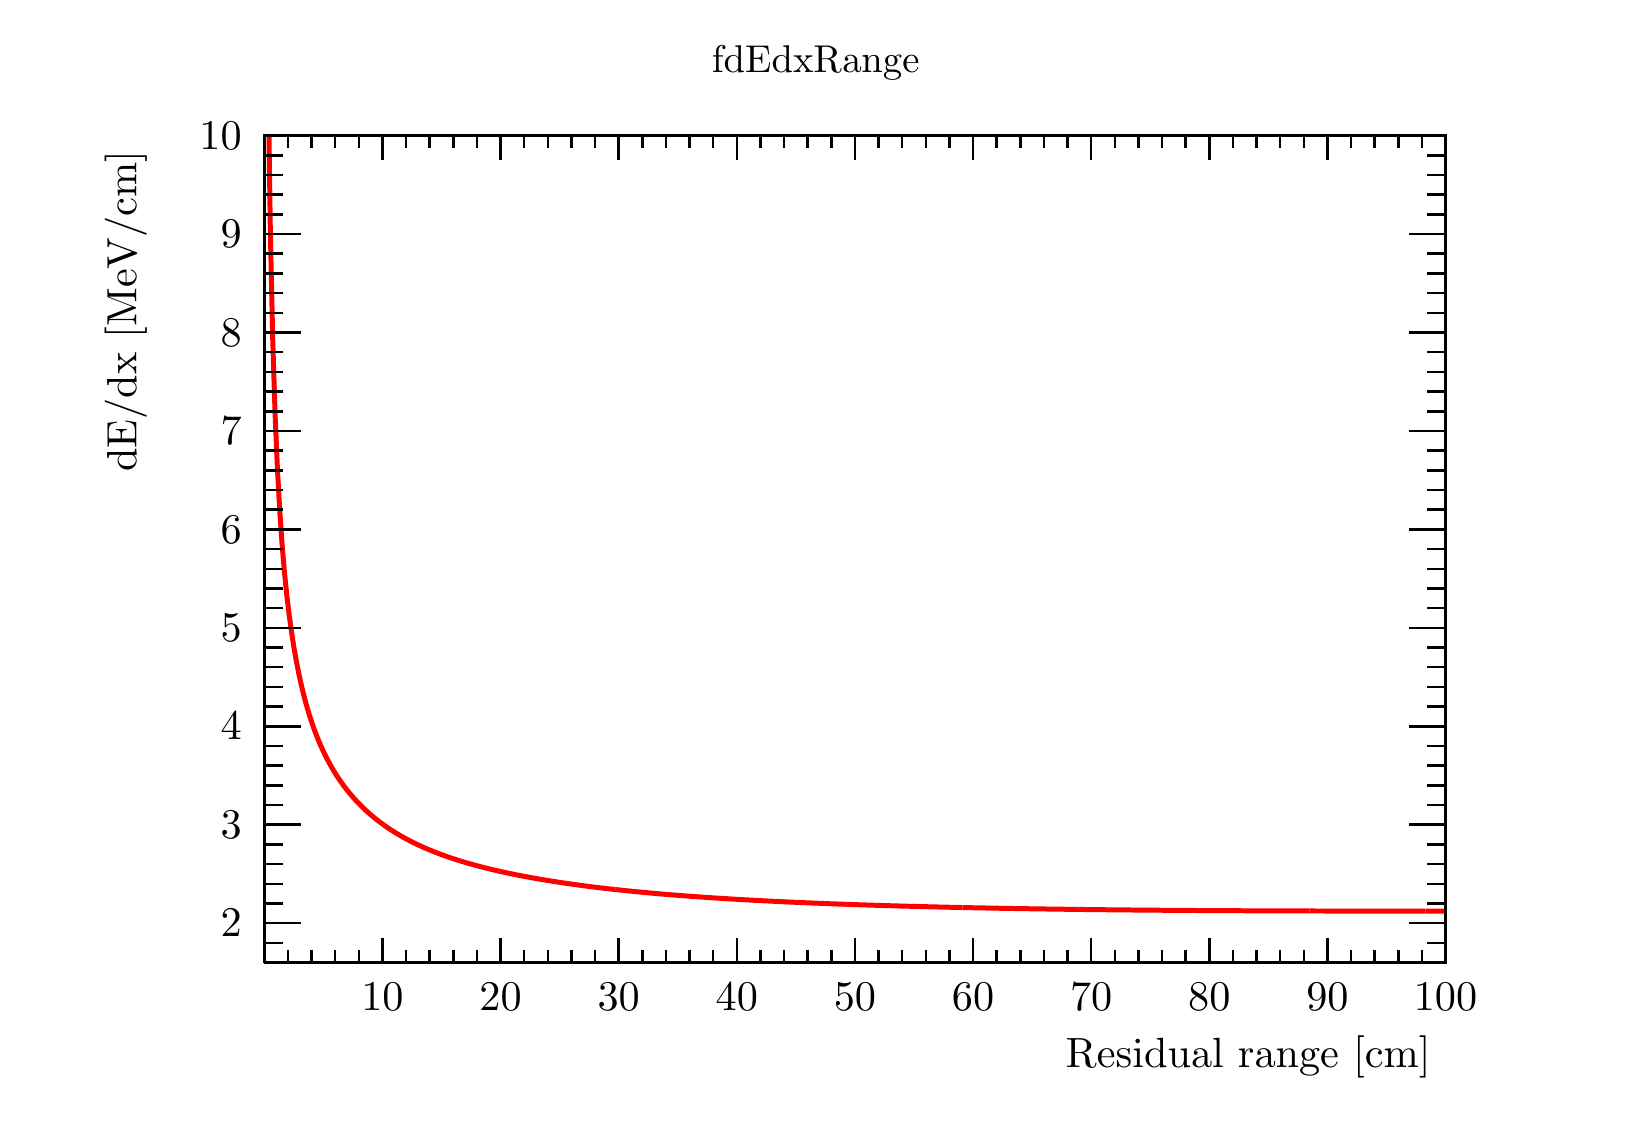
\begin{tikzpicture}
\pgfdeclareplotmark{cross} {
\pgfpathmoveto{\pgfpoint{-0.3\pgfplotmarksize}{\pgfplotmarksize}}
\pgfpathlineto{\pgfpoint{+0.3\pgfplotmarksize}{\pgfplotmarksize}}
\pgfpathlineto{\pgfpoint{+0.3\pgfplotmarksize}{0.3\pgfplotmarksize}}
\pgfpathlineto{\pgfpoint{+1\pgfplotmarksize}{0.3\pgfplotmarksize}}
\pgfpathlineto{\pgfpoint{+1\pgfplotmarksize}{-0.3\pgfplotmarksize}}
\pgfpathlineto{\pgfpoint{+0.3\pgfplotmarksize}{-0.3\pgfplotmarksize}}
\pgfpathlineto{\pgfpoint{+0.3\pgfplotmarksize}{-1.\pgfplotmarksize}}
\pgfpathlineto{\pgfpoint{-0.3\pgfplotmarksize}{-1.\pgfplotmarksize}}
\pgfpathlineto{\pgfpoint{-0.3\pgfplotmarksize}{-0.3\pgfplotmarksize}}
\pgfpathlineto{\pgfpoint{-1.\pgfplotmarksize}{-0.3\pgfplotmarksize}}
\pgfpathlineto{\pgfpoint{-1.\pgfplotmarksize}{0.3\pgfplotmarksize}}
\pgfpathlineto{\pgfpoint{-0.3\pgfplotmarksize}{0.3\pgfplotmarksize}}
\pgfpathclose
\pgfusepathqstroke
}
\pgfdeclareplotmark{cross*} {
\pgfpathmoveto{\pgfpoint{-0.3\pgfplotmarksize}{\pgfplotmarksize}}
\pgfpathlineto{\pgfpoint{+0.3\pgfplotmarksize}{\pgfplotmarksize}}
\pgfpathlineto{\pgfpoint{+0.3\pgfplotmarksize}{0.3\pgfplotmarksize}}
\pgfpathlineto{\pgfpoint{+1\pgfplotmarksize}{0.3\pgfplotmarksize}}
\pgfpathlineto{\pgfpoint{+1\pgfplotmarksize}{-0.3\pgfplotmarksize}}
\pgfpathlineto{\pgfpoint{+0.3\pgfplotmarksize}{-0.3\pgfplotmarksize}}
\pgfpathlineto{\pgfpoint{+0.3\pgfplotmarksize}{-1.\pgfplotmarksize}}
\pgfpathlineto{\pgfpoint{-0.3\pgfplotmarksize}{-1.\pgfplotmarksize}}
\pgfpathlineto{\pgfpoint{-0.3\pgfplotmarksize}{-0.3\pgfplotmarksize}}
\pgfpathlineto{\pgfpoint{-1.\pgfplotmarksize}{-0.3\pgfplotmarksize}}
\pgfpathlineto{\pgfpoint{-1.\pgfplotmarksize}{0.3\pgfplotmarksize}}
\pgfpathlineto{\pgfpoint{-0.3\pgfplotmarksize}{0.3\pgfplotmarksize}}
\pgfpathclose
\pgfusepathqfillstroke
}
\pgfdeclareplotmark{newstar} {
\pgfpathmoveto{\pgfqpoint{0pt}{\pgfplotmarksize}}
\pgfpathlineto{\pgfqpointpolar{44}{0.5\pgfplotmarksize}}
\pgfpathlineto{\pgfqpointpolar{18}{\pgfplotmarksize}}
\pgfpathlineto{\pgfqpointpolar{-20}{0.5\pgfplotmarksize}}
\pgfpathlineto{\pgfqpointpolar{-54}{\pgfplotmarksize}}
\pgfpathlineto{\pgfqpointpolar{-90}{0.5\pgfplotmarksize}}
\pgfpathlineto{\pgfqpointpolar{234}{\pgfplotmarksize}}
\pgfpathlineto{\pgfqpointpolar{198}{0.5\pgfplotmarksize}}
\pgfpathlineto{\pgfqpointpolar{162}{\pgfplotmarksize}}
\pgfpathlineto{\pgfqpointpolar{134}{0.5\pgfplotmarksize}}
\pgfpathclose
\pgfusepathqstroke
}
\pgfdeclareplotmark{newstar*} {
\pgfpathmoveto{\pgfqpoint{0pt}{\pgfplotmarksize}}
\pgfpathlineto{\pgfqpointpolar{44}{0.5\pgfplotmarksize}}
\pgfpathlineto{\pgfqpointpolar{18}{\pgfplotmarksize}}
\pgfpathlineto{\pgfqpointpolar{-20}{0.5\pgfplotmarksize}}
\pgfpathlineto{\pgfqpointpolar{-54}{\pgfplotmarksize}}
\pgfpathlineto{\pgfqpointpolar{-90}{0.5\pgfplotmarksize}}
\pgfpathlineto{\pgfqpointpolar{234}{\pgfplotmarksize}}
\pgfpathlineto{\pgfqpointpolar{198}{0.5\pgfplotmarksize}}
\pgfpathlineto{\pgfqpointpolar{162}{\pgfplotmarksize}}
\pgfpathlineto{\pgfqpointpolar{134}{0.5\pgfplotmarksize}}
\pgfpathclose
\pgfusepathqfillstroke
}
\definecolor{c}{rgb}{1,1,1};
\draw [color=c, fill=c] (0,0) rectangle (20,13.639);
\draw [color=c, fill=c] (3,1.77307) rectangle (18,12.2751);
\definecolor{c}{rgb}{0,0,0};
\draw [c,line width=0.9] (3,1.77307) -- (3,12.2751) -- (18,12.2751) -- (18,1.77307) -- (3,1.77307);
\definecolor{c}{rgb}{1,1,1};
\draw [color=c, fill=c] (3,1.77307) rectangle (18,12.2751);
\definecolor{c}{rgb}{0,0,0};
\draw [c,line width=0.9] (3,1.77307) -- (3,12.2751) -- (18,12.2751) -- (18,1.77307) -- (3,1.77307);
\definecolor{c}{rgb}{1,0,0};
\draw [c,line width=1.8] (3.05761,12.2751) -- (3.075,11.0517);
\draw [c,line width=1.8] (3.075,11.0517) -- (3.105,9.69138) -- (3.135,8.74094) -- (3.165,8.03897) -- (3.195,7.49881) -- (3.225,7.06959) -- (3.255,6.71937) -- (3.285,6.42706) -- (3.315,6.17811) -- (3.345,5.96213) -- (3.375,5.77157) -- (3.405,5.60162)
 -- (3.435,5.44905) -- (3.465,5.31128) -- (3.495,5.18619) -- (3.525,5.07206) -- (3.555,4.96743) -- (3.585,4.87111) -- (3.615,4.78206) -- (3.645,4.69943) -- (3.675,4.62245) -- (3.705,4.5505) -- (3.735,4.48303) -- (3.765,4.4196) -- (3.795,4.35985) --
 (3.825,4.30345) -- (3.855,4.25011) -- (3.885,4.19956) -- (3.915,4.15159) -- (3.945,4.10598) -- (3.975,4.06255) -- (4.005,4.02111) -- (4.035,3.98153) -- (4.065,3.94366) -- (4.095,3.90737) -- (4.125,3.87256) -- (4.155,3.83911) -- (4.185,3.80694) --
 (4.215,3.77598) -- (4.245,3.74616) -- (4.275,3.71743) -- (4.305,3.68973) -- (4.335,3.663) -- (4.365,3.63719) -- (4.395,3.61227) -- (4.425,3.58818) -- (4.455,3.56488) -- (4.485,3.54234) -- (4.515,3.52053);
\draw [c,line width=1.8] (4.515,3.52053) -- (4.545,3.4994) -- (4.575,3.47893) -- (4.605,3.45908) -- (4.635,3.43984) -- (4.665,3.42117) -- (4.695,3.40305) -- (4.725,3.38545) -- (4.755,3.36835) -- (4.785,3.35174) -- (4.815,3.33559) -- (4.845,3.31988)
 -- (4.875,3.3046) -- (4.905,3.28973) -- (4.935,3.27524) -- (4.965,3.26114) -- (4.995,3.2474) -- (5.025,3.23401) -- (5.055,3.22095) -- (5.085,3.20822) -- (5.115,3.1958) -- (5.145,3.18367) -- (5.175,3.17184) -- (5.205,3.16029) -- (5.235,3.149) --
 (5.265,3.13798) -- (5.295,3.12721) -- (5.325,3.11667) -- (5.355,3.10637) -- (5.385,3.0963) -- (5.415,3.08645) -- (5.445,3.07681) -- (5.475,3.06737) -- (5.505,3.05813) -- (5.535,3.04908) -- (5.565,3.04021) -- (5.595,3.03153) -- (5.625,3.02301) --
 (5.655,3.01467) -- (5.685,3.00649) -- (5.715,2.99846) -- (5.745,2.99059) -- (5.775,2.98287) -- (5.805,2.97529) -- (5.835,2.96786) -- (5.865,2.96055) -- (5.895,2.95338) -- (5.925,2.94634) -- (5.955,2.93942) -- (5.985,2.93262);
\draw [c,line width=1.8] (5.985,2.93262) -- (6.015,2.92594) -- (6.045,2.91937) -- (6.075,2.91291) -- (6.105,2.90656) -- (6.135,2.90032) -- (6.165,2.89417) -- (6.195,2.88813) -- (6.225,2.88218) -- (6.255,2.87632) -- (6.285,2.87056) -- (6.315,2.86488)
 -- (6.345,2.8593) -- (6.375,2.85379) -- (6.405,2.84837) -- (6.435,2.84303) -- (6.465,2.83777) -- (6.495,2.83259) -- (6.525,2.82748) -- (6.555,2.82245) -- (6.585,2.81749) -- (6.615,2.81261) -- (6.645,2.8078) -- (6.675,2.80306) -- (6.705,2.79838) --
 (6.735,2.79377) -- (6.765,2.78923) -- (6.795,2.78476) -- (6.825,2.78034) -- (6.855,2.776) -- (6.885,2.77171) -- (6.915,2.76748) -- (6.945,2.76331) -- (6.975,2.7592) -- (7.005,2.75515) -- (7.035,2.75115) -- (7.065,2.74721) -- (7.095,2.74332) --
 (7.125,2.73948) -- (7.155,2.7357) -- (7.185,2.73197) -- (7.215,2.72829) -- (7.245,2.72466) -- (7.275,2.72108) -- (7.305,2.71755) -- (7.335,2.71406) -- (7.365,2.71062) -- (7.395,2.70723) -- (7.425,2.70388) -- (7.455,2.70058);
\draw [c,line width=1.8] (7.455,2.70058) -- (7.485,2.69732) -- (7.515,2.6941) -- (7.545,2.69092) -- (7.575,2.68779) -- (7.605,2.6847) -- (7.635,2.68164) -- (7.665,2.67863) -- (7.695,2.67565) -- (7.725,2.67272) -- (7.755,2.66982) -- (7.785,2.66696) --
 (7.815,2.66413) -- (7.845,2.66134) -- (7.875,2.65858) -- (7.905,2.65586) -- (7.935,2.65318) -- (7.965,2.65053) -- (7.995,2.64791) -- (8.025,2.64532) -- (8.055,2.64276) -- (8.085,2.64024) -- (8.115,2.63775) -- (8.145,2.63528) -- (8.175,2.63285) --
 (8.205,2.63045) -- (8.235,2.62807) -- (8.265,2.62573) -- (8.295,2.62341) -- (8.325,2.62112) -- (8.355,2.61886) -- (8.385,2.61662) -- (8.415,2.61441) -- (8.445,2.61223) -- (8.475,2.61008) -- (8.505,2.60794) -- (8.535,2.60584) -- (8.565,2.60376) --
 (8.595,2.6017) -- (8.625,2.59967) -- (8.655,2.59766) -- (8.685,2.59567) -- (8.715,2.59371) -- (8.745,2.59177) -- (8.775,2.58985) -- (8.805,2.58795) -- (8.835,2.58608) -- (8.865,2.58422) -- (8.895,2.58239) -- (8.925,2.58058);
\draw [c,line width=1.8] (8.925,2.58058) -- (8.955,2.57879) -- (8.985,2.57702) -- (9.015,2.57527) -- (9.045,2.57354) -- (9.075,2.57182) -- (9.105,2.57013) -- (9.135,2.56846) -- (9.165,2.5668) -- (9.195,2.56517) -- (9.225,2.56355) -- (9.255,2.56195)
 -- (9.285,2.56036) -- (9.315,2.5588) -- (9.345,2.55725) -- (9.375,2.55572) -- (9.405,2.5542) -- (9.435,2.5527) -- (9.465,2.55122) -- (9.495,2.54975) -- (9.525,2.5483) -- (9.555,2.54687) -- (9.585,2.54545) -- (9.615,2.54405) -- (9.645,2.54266) --
 (9.675,2.54129) -- (9.705,2.53993) -- (9.735,2.53858) -- (9.765,2.53725) -- (9.795,2.53594) -- (9.825,2.53463) -- (9.855,2.53335) -- (9.885,2.53207) -- (9.915,2.53081) -- (9.945,2.52956) -- (9.975,2.52833) -- (10.005,2.52711) -- (10.035,2.5259) --
 (10.065,2.5247) -- (10.095,2.52352) -- (10.125,2.52235) -- (10.155,2.52119) -- (10.185,2.52005) -- (10.215,2.51891) -- (10.245,2.51779) -- (10.275,2.51668) -- (10.305,2.51558) -- (10.335,2.51449) -- (10.365,2.51342) -- (10.395,2.51235);
\draw [c,line width=1.8] (10.395,2.51235) -- (10.425,2.5113) -- (10.455,2.51025) -- (10.485,2.50922) -- (10.515,2.5082) -- (10.545,2.50719) -- (10.575,2.50619) -- (10.605,2.5052) -- (10.635,2.50422) -- (10.665,2.50325) -- (10.695,2.50229) --
 (10.725,2.50134) -- (10.755,2.5004) -- (10.785,2.49947) -- (10.815,2.49855) -- (10.845,2.49764) -- (10.875,2.49674) -- (10.905,2.49584) -- (10.935,2.49496) -- (10.965,2.49409) -- (10.995,2.49322) -- (11.025,2.49237) -- (11.055,2.49152) --
 (11.085,2.49068) -- (11.115,2.48986) -- (11.145,2.48903) -- (11.175,2.48822) -- (11.205,2.48742) -- (11.235,2.48662) -- (11.265,2.48584) -- (11.295,2.48506) -- (11.325,2.48429) -- (11.355,2.48353) -- (11.385,2.48277) -- (11.415,2.48203) --
 (11.445,2.48129) -- (11.475,2.48056) -- (11.505,2.47983) -- (11.535,2.47912) -- (11.565,2.47841) -- (11.595,2.47771) -- (11.625,2.47701) -- (11.655,2.47633) -- (11.685,2.47565) -- (11.715,2.47498) -- (11.745,2.47431) -- (11.775,2.47366) --
 (11.805,2.473) -- (11.835,2.47236) -- (11.865,2.47172);
\draw [c,line width=1.8] (11.865,2.47172) -- (11.895,2.47109) -- (11.925,2.47047) -- (11.955,2.46985) -- (11.985,2.46924) -- (12.015,2.46864) -- (12.045,2.46804) -- (12.075,2.46745) -- (12.105,2.46687) -- (12.135,2.46629) -- (12.165,2.46572) --
 (12.195,2.46515) -- (12.225,2.46459) -- (12.255,2.46404) -- (12.285,2.46349) -- (12.315,2.46295) -- (12.345,2.46241) -- (12.375,2.46188) -- (12.405,2.46135) -- (12.435,2.46084) -- (12.465,2.46032) -- (12.495,2.45982) -- (12.525,2.45931) --
 (12.555,2.45882) -- (12.585,2.45833) -- (12.615,2.45784) -- (12.645,2.45736) -- (12.675,2.45689) -- (12.705,2.45642) -- (12.735,2.45595) -- (12.765,2.45549) -- (12.795,2.45504) -- (12.825,2.45459) -- (12.855,2.45414) -- (12.885,2.45371) --
 (12.915,2.45327) -- (12.945,2.45284) -- (12.975,2.45242) -- (13.005,2.452) -- (13.035,2.45158) -- (13.065,2.45117) -- (13.095,2.45077) -- (13.125,2.45037) -- (13.155,2.44997) -- (13.185,2.44958) -- (13.215,2.44919) -- (13.245,2.44881) --
 (13.275,2.44843) -- (13.305,2.44806) -- (13.335,2.44769);
\draw [c,line width=1.8] (13.335,2.44769) -- (13.365,2.44733) -- (13.395,2.44697) -- (13.425,2.44661) -- (13.455,2.44626) -- (13.485,2.44591) -- (13.515,2.44557) -- (13.545,2.44523) -- (13.575,2.44489) -- (13.605,2.44456) -- (13.635,2.44423) --
 (13.665,2.44391) -- (13.695,2.44359) -- (13.725,2.44328) -- (13.755,2.44297) -- (13.785,2.44266) -- (13.815,2.44235) -- (13.845,2.44205) -- (13.875,2.44176) -- (13.905,2.44147) -- (13.935,2.44118) -- (13.965,2.44089) -- (13.995,2.44061) --
 (14.025,2.44033) -- (14.055,2.44006) -- (14.085,2.43979) -- (14.115,2.43952) -- (14.145,2.43926) -- (14.175,2.439) -- (14.205,2.43874) -- (14.235,2.43849) -- (14.265,2.43824) -- (14.295,2.43799) -- (14.325,2.43775) -- (14.355,2.43751) --
 (14.385,2.43727) -- (14.415,2.43704) -- (14.445,2.43681) -- (14.475,2.43658) -- (14.505,2.43636) -- (14.535,2.43614) -- (14.565,2.43592) -- (14.595,2.43571) -- (14.625,2.4355) -- (14.655,2.43529) -- (14.685,2.43508) -- (14.715,2.43488) --
 (14.745,2.43468) -- (14.775,2.43449) -- (14.805,2.43429);
\draw [c,line width=1.8] (14.805,2.43429) -- (14.835,2.4341) -- (14.865,2.43392) -- (14.895,2.43373) -- (14.925,2.43355) -- (14.955,2.43337) -- (14.985,2.4332) -- (15.015,2.43302) -- (15.045,2.43285) -- (15.075,2.43269) -- (15.105,2.43252) --
 (15.135,2.43236) -- (15.165,2.4322) -- (15.195,2.43204) -- (15.225,2.43189) -- (15.255,2.43174) -- (15.285,2.43159) -- (15.315,2.43144) -- (15.345,2.4313) -- (15.375,2.43116) -- (15.405,2.43102) -- (15.435,2.43088) -- (15.465,2.43075) --
 (15.495,2.43062) -- (15.525,2.43049) -- (15.555,2.43037) -- (15.585,2.43024) -- (15.615,2.43012) -- (15.645,2.43) -- (15.675,2.42989) -- (15.705,2.42977) -- (15.735,2.42966) -- (15.765,2.42955) -- (15.795,2.42944) -- (15.825,2.42934) --
 (15.855,2.42924) -- (15.885,2.42914) -- (15.915,2.42904) -- (15.945,2.42894) -- (15.975,2.42885) -- (16.005,2.42876) -- (16.035,2.42867) -- (16.065,2.42858) -- (16.095,2.4285) -- (16.125,2.42841) -- (16.155,2.42833) -- (16.185,2.42825) --
 (16.215,2.42818) -- (16.245,2.4281) -- (16.275,2.42803);
\draw [c,line width=1.8] (16.275,2.42803) -- (16.305,2.42796) -- (16.335,2.42789) -- (16.365,2.42782) -- (16.395,2.42776) -- (16.425,2.4277) -- (16.455,2.42764) -- (16.485,2.42758) -- (16.515,2.42752) -- (16.545,2.42747) -- (16.575,2.42741) --
 (16.605,2.42736) -- (16.635,2.42731) -- (16.665,2.42727) -- (16.695,2.42722) -- (16.725,2.42718) -- (16.755,2.42714) -- (16.785,2.4271) -- (16.815,2.42706) -- (16.845,2.42702) -- (16.875,2.42699) -- (16.905,2.42696) -- (16.935,2.42693) --
 (16.965,2.4269) -- (16.995,2.42687) -- (17.025,2.42684) -- (17.055,2.42682) -- (17.085,2.4268) -- (17.115,2.42678) -- (17.145,2.42676) -- (17.175,2.42674) -- (17.205,2.42673) -- (17.235,2.42671) -- (17.265,2.4267) -- (17.295,2.42669) --
 (17.325,2.42668) -- (17.355,2.42667) -- (17.385,2.42667) -- (17.415,2.42666) -- (17.445,2.42666) -- (17.475,2.42666) -- (17.505,2.42666) -- (17.535,2.42666) -- (17.565,2.42666) -- (17.595,2.42667) -- (17.625,2.42668) -- (17.655,2.42668) --
 (17.685,2.42669) -- (17.715,2.4267) -- (17.745,2.42672);
\draw [c,line width=1.8] (17.745,2.42672) -- (17.775,2.42673) -- (17.805,2.42674) -- (17.835,2.42676) -- (17.865,2.42678) -- (17.895,2.4268) -- (17.925,2.42682) -- (17.955,2.42684) -- (17.985,2.42686);
\definecolor{c}{rgb}{0,0,0};
\draw [c,line width=0.9] (3,1.77307) -- (18,1.77307);
\draw [c,line width=0.9] (4.49865,2.07994) -- (4.49865,1.77307);
\draw [c,line width=0.9] (4.79868,1.9265) -- (4.79868,1.77307);
\draw [c,line width=0.9] (5.09871,1.9265) -- (5.09871,1.77307);
\draw [c,line width=0.9] (5.39874,1.9265) -- (5.39874,1.77307);
\draw [c,line width=0.9] (5.69877,1.9265) -- (5.69877,1.77307);
\draw [c,line width=0.9] (5.9988,2.07994) -- (5.9988,1.77307);
\draw [c,line width=0.9] (6.29883,1.9265) -- (6.29883,1.77307);
\draw [c,line width=0.9] (6.59886,1.9265) -- (6.59886,1.77307);
\draw [c,line width=0.9] (6.89889,1.9265) -- (6.89889,1.77307);
\draw [c,line width=0.9] (7.19892,1.9265) -- (7.19892,1.77307);
\draw [c,line width=0.9] (7.49895,2.07994) -- (7.49895,1.77307);
\draw [c,line width=0.9] (7.79898,1.9265) -- (7.79898,1.77307);
\draw [c,line width=0.9] (8.09901,1.9265) -- (8.09901,1.77307);
\draw [c,line width=0.9] (8.39904,1.9265) -- (8.39904,1.77307);
\draw [c,line width=0.9] (8.69907,1.9265) -- (8.69907,1.77307);
\draw [c,line width=0.9] (8.9991,2.07994) -- (8.9991,1.77307);
\draw [c,line width=0.9] (9.29913,1.9265) -- (9.29913,1.77307);
\draw [c,line width=0.9] (9.59916,1.9265) -- (9.59916,1.77307);
\draw [c,line width=0.9] (9.89919,1.9265) -- (9.89919,1.77307);
\draw [c,line width=0.9] (10.1992,1.9265) -- (10.1992,1.77307);
\draw [c,line width=0.9] (10.4993,2.07994) -- (10.4993,1.77307);
\draw [c,line width=0.9] (10.7993,1.9265) -- (10.7993,1.77307);
\draw [c,line width=0.9] (11.0993,1.9265) -- (11.0993,1.77307);
\draw [c,line width=0.9] (11.3993,1.9265) -- (11.3993,1.77307);
\draw [c,line width=0.9] (11.6994,1.9265) -- (11.6994,1.77307);
\draw [c,line width=0.9] (11.9994,2.07994) -- (11.9994,1.77307);
\draw [c,line width=0.9] (12.2994,1.9265) -- (12.2994,1.77307);
\draw [c,line width=0.9] (12.5995,1.9265) -- (12.5995,1.77307);
\draw [c,line width=0.9] (12.8995,1.9265) -- (12.8995,1.77307);
\draw [c,line width=0.9] (13.1995,1.9265) -- (13.1995,1.77307);
\draw [c,line width=0.9] (13.4995,2.07994) -- (13.4995,1.77307);
\draw [c,line width=0.9] (13.7996,1.9265) -- (13.7996,1.77307);
\draw [c,line width=0.9] (14.0996,1.9265) -- (14.0996,1.77307);
\draw [c,line width=0.9] (14.3996,1.9265) -- (14.3996,1.77307);
\draw [c,line width=0.9] (14.6997,1.9265) -- (14.6997,1.77307);
\draw [c,line width=0.9] (14.9997,2.07994) -- (14.9997,1.77307);
\draw [c,line width=0.9] (15.2997,1.9265) -- (15.2997,1.77307);
\draw [c,line width=0.9] (15.5998,1.9265) -- (15.5998,1.77307);
\draw [c,line width=0.9] (15.8998,1.9265) -- (15.8998,1.77307);
\draw [c,line width=0.9] (16.1998,1.9265) -- (16.1998,1.77307);
\draw [c,line width=0.9] (16.4998,2.07994) -- (16.4998,1.77307);
\draw [c,line width=0.9] (16.7999,1.9265) -- (16.7999,1.77307);
\draw [c,line width=0.9] (17.0999,1.9265) -- (17.0999,1.77307);
\draw [c,line width=0.9] (17.3999,1.9265) -- (17.3999,1.77307);
\draw [c,line width=0.9] (17.7,1.9265) -- (17.7,1.77307);
\draw [c,line width=0.9] (18,2.07994) -- (18,1.77307);
\draw [c,line width=0.9] (4.49865,2.07994) -- (4.49865,1.77307);
\draw [c,line width=0.9] (4.19862,1.9265) -- (4.19862,1.77307);
\draw [c,line width=0.9] (3.89859,1.9265) -- (3.89859,1.77307);
\draw [c,line width=0.9] (3.59856,1.9265) -- (3.59856,1.77307);
\draw [c,line width=0.9] (3.29853,1.9265) -- (3.29853,1.77307);
\draw [anchor=base] (4.49865,1.15931) node[scale=1.52731, color=c, rotate=0]{10};
\draw [anchor=base] (5.9988,1.15931) node[scale=1.52731, color=c, rotate=0]{20};
\draw [anchor=base] (7.49895,1.15931) node[scale=1.52731, color=c, rotate=0]{30};
\draw [anchor=base] (8.9991,1.15931) node[scale=1.52731, color=c, rotate=0]{40};
\draw [anchor=base] (10.4993,1.15931) node[scale=1.52731, color=c, rotate=0]{50};
\draw [anchor=base] (11.9994,1.15931) node[scale=1.52731, color=c, rotate=0]{60};
\draw [anchor=base] (13.4995,1.15931) node[scale=1.52731, color=c, rotate=0]{70};
\draw [anchor=base] (14.9997,1.15931) node[scale=1.52731, color=c, rotate=0]{80};
\draw [anchor=base] (16.4998,1.15931) node[scale=1.52731, color=c, rotate=0]{90};
\draw [anchor=base] (18,1.15931) node[scale=1.52731, color=c, rotate=0]{100};
\draw [anchor= east] (18,0.572837) node[scale=1.52731, color=c, rotate=0]{Residual range [cm]};
\draw [c,line width=0.9] (3,12.2751) -- (18,12.2751);
\draw [c,line width=0.9] (4.49865,11.9682) -- (4.49865,12.2751);
\draw [c,line width=0.9] (4.79868,12.1216) -- (4.79868,12.2751);
\draw [c,line width=0.9] (5.09871,12.1216) -- (5.09871,12.2751);
\draw [c,line width=0.9] (5.39874,12.1216) -- (5.39874,12.2751);
\draw [c,line width=0.9] (5.69877,12.1216) -- (5.69877,12.2751);
\draw [c,line width=0.9] (5.9988,11.9682) -- (5.9988,12.2751);
\draw [c,line width=0.9] (6.29883,12.1216) -- (6.29883,12.2751);
\draw [c,line width=0.9] (6.59886,12.1216) -- (6.59886,12.2751);
\draw [c,line width=0.9] (6.89889,12.1216) -- (6.89889,12.2751);
\draw [c,line width=0.9] (7.19892,12.1216) -- (7.19892,12.2751);
\draw [c,line width=0.9] (7.49895,11.9682) -- (7.49895,12.2751);
\draw [c,line width=0.9] (7.79898,12.1216) -- (7.79898,12.2751);
\draw [c,line width=0.9] (8.09901,12.1216) -- (8.09901,12.2751);
\draw [c,line width=0.9] (8.39904,12.1216) -- (8.39904,12.2751);
\draw [c,line width=0.9] (8.69907,12.1216) -- (8.69907,12.2751);
\draw [c,line width=0.9] (8.9991,11.9682) -- (8.9991,12.2751);
\draw [c,line width=0.9] (9.29913,12.1216) -- (9.29913,12.2751);
\draw [c,line width=0.9] (9.59916,12.1216) -- (9.59916,12.2751);
\draw [c,line width=0.9] (9.89919,12.1216) -- (9.89919,12.2751);
\draw [c,line width=0.9] (10.1992,12.1216) -- (10.1992,12.2751);
\draw [c,line width=0.9] (10.4993,11.9682) -- (10.4993,12.2751);
\draw [c,line width=0.9] (10.7993,12.1216) -- (10.7993,12.2751);
\draw [c,line width=0.9] (11.0993,12.1216) -- (11.0993,12.2751);
\draw [c,line width=0.9] (11.3993,12.1216) -- (11.3993,12.2751);
\draw [c,line width=0.9] (11.6994,12.1216) -- (11.6994,12.2751);
\draw [c,line width=0.9] (11.9994,11.9682) -- (11.9994,12.2751);
\draw [c,line width=0.9] (12.2994,12.1216) -- (12.2994,12.2751);
\draw [c,line width=0.9] (12.5995,12.1216) -- (12.5995,12.2751);
\draw [c,line width=0.9] (12.8995,12.1216) -- (12.8995,12.2751);
\draw [c,line width=0.9] (13.1995,12.1216) -- (13.1995,12.2751);
\draw [c,line width=0.9] (13.4995,11.9682) -- (13.4995,12.2751);
\draw [c,line width=0.9] (13.7996,12.1216) -- (13.7996,12.2751);
\draw [c,line width=0.9] (14.0996,12.1216) -- (14.0996,12.2751);
\draw [c,line width=0.9] (14.3996,12.1216) -- (14.3996,12.2751);
\draw [c,line width=0.9] (14.6997,12.1216) -- (14.6997,12.2751);
\draw [c,line width=0.9] (14.9997,11.9682) -- (14.9997,12.2751);
\draw [c,line width=0.9] (15.2997,12.1216) -- (15.2997,12.2751);
\draw [c,line width=0.9] (15.5998,12.1216) -- (15.5998,12.2751);
\draw [c,line width=0.9] (15.8998,12.1216) -- (15.8998,12.2751);
\draw [c,line width=0.9] (16.1998,12.1216) -- (16.1998,12.2751);
\draw [c,line width=0.9] (16.4998,11.9682) -- (16.4998,12.2751);
\draw [c,line width=0.9] (16.7999,12.1216) -- (16.7999,12.2751);
\draw [c,line width=0.9] (17.0999,12.1216) -- (17.0999,12.2751);
\draw [c,line width=0.9] (17.3999,12.1216) -- (17.3999,12.2751);
\draw [c,line width=0.9] (17.7,12.1216) -- (17.7,12.2751);
\draw [c,line width=0.9] (18,11.9682) -- (18,12.2751);
\draw [c,line width=0.9] (4.49865,11.9682) -- (4.49865,12.2751);
\draw [c,line width=0.9] (4.19862,12.1216) -- (4.19862,12.2751);
\draw [c,line width=0.9] (3.89859,12.1216) -- (3.89859,12.2751);
\draw [c,line width=0.9] (3.59856,12.1216) -- (3.59856,12.2751);
\draw [c,line width=0.9] (3.29853,12.1216) -- (3.29853,12.2751);
\draw [c,line width=0.9] (3,1.77307) -- (3,12.2751);
\draw [c,line width=0.9] (3.462,2.27316) -- (3,2.27316);
\draw [c,line width=0.9] (3.231,2.52321) -- (3,2.52321);
\draw [c,line width=0.9] (3.231,2.77326) -- (3,2.77326);
\draw [c,line width=0.9] (3.231,3.0233) -- (3,3.0233);
\draw [c,line width=0.9] (3.231,3.27335) -- (3,3.27335);
\draw [c,line width=0.9] (3.462,3.5234) -- (3,3.5234);
\draw [c,line width=0.9] (3.231,3.77345) -- (3,3.77345);
\draw [c,line width=0.9] (3.231,4.0235) -- (3,4.0235);
\draw [c,line width=0.9] (3.231,4.27354) -- (3,4.27354);
\draw [c,line width=0.9] (3.231,4.52359) -- (3,4.52359);
\draw [c,line width=0.9] (3.462,4.77364) -- (3,4.77364);
\draw [c,line width=0.9] (3.231,5.02369) -- (3,5.02369);
\draw [c,line width=0.9] (3.231,5.27373) -- (3,5.27373);
\draw [c,line width=0.9] (3.231,5.52378) -- (3,5.52378);
\draw [c,line width=0.9] (3.231,5.77383) -- (3,5.77383);
\draw [c,line width=0.9] (3.462,6.02388) -- (3,6.02388);
\draw [c,line width=0.9] (3.231,6.27393) -- (3,6.27393);
\draw [c,line width=0.9] (3.231,6.52397) -- (3,6.52397);
\draw [c,line width=0.9] (3.231,6.77402) -- (3,6.77402);
\draw [c,line width=0.9] (3.231,7.02407) -- (3,7.02407);
\draw [c,line width=0.9] (3.462,7.27412) -- (3,7.27412);
\draw [c,line width=0.9] (3.231,7.52416) -- (3,7.52416);
\draw [c,line width=0.9] (3.231,7.77421) -- (3,7.77421);
\draw [c,line width=0.9] (3.231,8.02426) -- (3,8.02426);
\draw [c,line width=0.9] (3.231,8.27431) -- (3,8.27431);
\draw [c,line width=0.9] (3.462,8.52435) -- (3,8.52435);
\draw [c,line width=0.9] (3.231,8.7744) -- (3,8.7744);
\draw [c,line width=0.9] (3.231,9.02445) -- (3,9.02445);
\draw [c,line width=0.9] (3.231,9.2745) -- (3,9.2745);
\draw [c,line width=0.9] (3.231,9.52455) -- (3,9.52455);
\draw [c,line width=0.9] (3.462,9.77459) -- (3,9.77459);
\draw [c,line width=0.9] (3.231,10.0246) -- (3,10.0246);
\draw [c,line width=0.9] (3.231,10.2747) -- (3,10.2747);
\draw [c,line width=0.9] (3.231,10.5247) -- (3,10.5247);
\draw [c,line width=0.9] (3.231,10.7748) -- (3,10.7748);
\draw [c,line width=0.9] (3.462,11.0248) -- (3,11.0248);
\draw [c,line width=0.9] (3.231,11.2749) -- (3,11.2749);
\draw [c,line width=0.9] (3.231,11.5249) -- (3,11.5249);
\draw [c,line width=0.9] (3.231,11.775) -- (3,11.775);
\draw [c,line width=0.9] (3.231,12.025) -- (3,12.025);
\draw [c,line width=0.9] (3.462,12.2751) -- (3,12.2751);
\draw [c,line width=0.9] (3.462,2.27316) -- (3,2.27316);
\draw [c,line width=0.9] (3.231,2.02311) -- (3,2.02311);
\draw [c,line width=0.9] (3.231,1.77307) -- (3,1.77307);
\draw [anchor= east] (2.9,2.27316) node[scale=1.52731, color=c, rotate=0]{2};
\draw [anchor= east] (2.9,3.5234) node[scale=1.52731, color=c, rotate=0]{3};
\draw [anchor= east] (2.9,4.77364) node[scale=1.52731, color=c, rotate=0]{4};
\draw [anchor= east] (2.9,6.02388) node[scale=1.52731, color=c, rotate=0]{5};
\draw [anchor= east] (2.9,7.27412) node[scale=1.52731, color=c, rotate=0]{6};
\draw [anchor= east] (2.9,8.52435) node[scale=1.52731, color=c, rotate=0]{7};
\draw [anchor= east] (2.9,9.77459) node[scale=1.52731, color=c, rotate=0]{8};
\draw [anchor= east] (2.9,11.0248) node[scale=1.52731, color=c, rotate=0]{9};
\draw [anchor= east] (2.9,12.2751) node[scale=1.52731, color=c, rotate=0]{10};
\draw [anchor= east] (1.24,12.2751) node[scale=1.52731, color=c, rotate=90]{dE/dx [MeV/cm]};
\draw [c,line width=0.9] (18,1.77307) -- (18,12.2751);
\draw [c,line width=0.9] (17.538,2.27316) -- (18,2.27316);
\draw [c,line width=0.9] (17.769,2.52321) -- (18,2.52321);
\draw [c,line width=0.9] (17.769,2.77326) -- (18,2.77326);
\draw [c,line width=0.9] (17.769,3.0233) -- (18,3.0233);
\draw [c,line width=0.9] (17.769,3.27335) -- (18,3.27335);
\draw [c,line width=0.9] (17.538,3.5234) -- (18,3.5234);
\draw [c,line width=0.9] (17.769,3.77345) -- (18,3.77345);
\draw [c,line width=0.9] (17.769,4.0235) -- (18,4.0235);
\draw [c,line width=0.9] (17.769,4.27354) -- (18,4.27354);
\draw [c,line width=0.9] (17.769,4.52359) -- (18,4.52359);
\draw [c,line width=0.9] (17.538,4.77364) -- (18,4.77364);
\draw [c,line width=0.9] (17.769,5.02369) -- (18,5.02369);
\draw [c,line width=0.9] (17.769,5.27373) -- (18,5.27373);
\draw [c,line width=0.9] (17.769,5.52378) -- (18,5.52378);
\draw [c,line width=0.9] (17.769,5.77383) -- (18,5.77383);
\draw [c,line width=0.9] (17.538,6.02388) -- (18,6.02388);
\draw [c,line width=0.9] (17.769,6.27393) -- (18,6.27393);
\draw [c,line width=0.9] (17.769,6.52397) -- (18,6.52397);
\draw [c,line width=0.9] (17.769,6.77402) -- (18,6.77402);
\draw [c,line width=0.9] (17.769,7.02407) -- (18,7.02407);
\draw [c,line width=0.9] (17.538,7.27412) -- (18,7.27412);
\draw [c,line width=0.9] (17.769,7.52416) -- (18,7.52416);
\draw [c,line width=0.9] (17.769,7.77421) -- (18,7.77421);
\draw [c,line width=0.9] (17.769,8.02426) -- (18,8.02426);
\draw [c,line width=0.9] (17.769,8.27431) -- (18,8.27431);
\draw [c,line width=0.9] (17.538,8.52435) -- (18,8.52435);
\draw [c,line width=0.9] (17.769,8.7744) -- (18,8.7744);
\draw [c,line width=0.9] (17.769,9.02445) -- (18,9.02445);
\draw [c,line width=0.9] (17.769,9.2745) -- (18,9.2745);
\draw [c,line width=0.9] (17.769,9.52455) -- (18,9.52455);
\draw [c,line width=0.9] (17.538,9.77459) -- (18,9.77459);
\draw [c,line width=0.9] (17.769,10.0246) -- (18,10.0246);
\draw [c,line width=0.9] (17.769,10.2747) -- (18,10.2747);
\draw [c,line width=0.9] (17.769,10.5247) -- (18,10.5247);
\draw [c,line width=0.9] (17.769,10.7748) -- (18,10.7748);
\draw [c,line width=0.9] (17.538,11.0248) -- (18,11.0248);
\draw [c,line width=0.9] (17.769,11.2749) -- (18,11.2749);
\draw [c,line width=0.9] (17.769,11.5249) -- (18,11.5249);
\draw [c,line width=0.9] (17.769,11.775) -- (18,11.775);
\draw [c,line width=0.9] (17.769,12.025) -- (18,12.025);
\draw [c,line width=0.9] (17.538,12.2751) -- (18,12.2751);
\draw [c,line width=0.9] (17.538,2.27316) -- (18,2.27316);
\draw [c,line width=0.9] (17.769,2.02311) -- (18,2.02311);
\draw [c,line width=0.9] (17.769,1.77307) -- (18,1.77307);
\definecolor{c}{rgb}{1,1,1};
\draw [color=c, fill=c] (2,12.8206) rectangle (18,13.5708);
\definecolor{c}{rgb}{0,0,0};
\draw (10,13.1957) node[scale=1.40004, color=c, rotate=0]{fdEdxRange};
\end{tikzpicture}

		\end{adjustbox}
	\end{minipage}
	\hfill
	\begin{minipage}[t]{.5\linewidth}
		\begin{adjustbox}{max totalsize=\linewidth, center}
			\begin{tikzpicture}
\pgfdeclareplotmark{cross} {
\pgfpathmoveto{\pgfpoint{-0.3\pgfplotmarksize}{\pgfplotmarksize}}
\pgfpathlineto{\pgfpoint{+0.3\pgfplotmarksize}{\pgfplotmarksize}}
\pgfpathlineto{\pgfpoint{+0.3\pgfplotmarksize}{0.3\pgfplotmarksize}}
\pgfpathlineto{\pgfpoint{+1\pgfplotmarksize}{0.3\pgfplotmarksize}}
\pgfpathlineto{\pgfpoint{+1\pgfplotmarksize}{-0.3\pgfplotmarksize}}
\pgfpathlineto{\pgfpoint{+0.3\pgfplotmarksize}{-0.3\pgfplotmarksize}}
\pgfpathlineto{\pgfpoint{+0.3\pgfplotmarksize}{-1.\pgfplotmarksize}}
\pgfpathlineto{\pgfpoint{-0.3\pgfplotmarksize}{-1.\pgfplotmarksize}}
\pgfpathlineto{\pgfpoint{-0.3\pgfplotmarksize}{-0.3\pgfplotmarksize}}
\pgfpathlineto{\pgfpoint{-1.\pgfplotmarksize}{-0.3\pgfplotmarksize}}
\pgfpathlineto{\pgfpoint{-1.\pgfplotmarksize}{0.3\pgfplotmarksize}}
\pgfpathlineto{\pgfpoint{-0.3\pgfplotmarksize}{0.3\pgfplotmarksize}}
\pgfpathclose
\pgfusepathqstroke
}
\pgfdeclareplotmark{cross*} {
\pgfpathmoveto{\pgfpoint{-0.3\pgfplotmarksize}{\pgfplotmarksize}}
\pgfpathlineto{\pgfpoint{+0.3\pgfplotmarksize}{\pgfplotmarksize}}
\pgfpathlineto{\pgfpoint{+0.3\pgfplotmarksize}{0.3\pgfplotmarksize}}
\pgfpathlineto{\pgfpoint{+1\pgfplotmarksize}{0.3\pgfplotmarksize}}
\pgfpathlineto{\pgfpoint{+1\pgfplotmarksize}{-0.3\pgfplotmarksize}}
\pgfpathlineto{\pgfpoint{+0.3\pgfplotmarksize}{-0.3\pgfplotmarksize}}
\pgfpathlineto{\pgfpoint{+0.3\pgfplotmarksize}{-1.\pgfplotmarksize}}
\pgfpathlineto{\pgfpoint{-0.3\pgfplotmarksize}{-1.\pgfplotmarksize}}
\pgfpathlineto{\pgfpoint{-0.3\pgfplotmarksize}{-0.3\pgfplotmarksize}}
\pgfpathlineto{\pgfpoint{-1.\pgfplotmarksize}{-0.3\pgfplotmarksize}}
\pgfpathlineto{\pgfpoint{-1.\pgfplotmarksize}{0.3\pgfplotmarksize}}
\pgfpathlineto{\pgfpoint{-0.3\pgfplotmarksize}{0.3\pgfplotmarksize}}
\pgfpathclose
\pgfusepathqfillstroke
}
\pgfdeclareplotmark{newstar} {
\pgfpathmoveto{\pgfqpoint{0pt}{\pgfplotmarksize}}
\pgfpathlineto{\pgfqpointpolar{44}{0.5\pgfplotmarksize}}
\pgfpathlineto{\pgfqpointpolar{18}{\pgfplotmarksize}}
\pgfpathlineto{\pgfqpointpolar{-20}{0.5\pgfplotmarksize}}
\pgfpathlineto{\pgfqpointpolar{-54}{\pgfplotmarksize}}
\pgfpathlineto{\pgfqpointpolar{-90}{0.5\pgfplotmarksize}}
\pgfpathlineto{\pgfqpointpolar{234}{\pgfplotmarksize}}
\pgfpathlineto{\pgfqpointpolar{198}{0.5\pgfplotmarksize}}
\pgfpathlineto{\pgfqpointpolar{162}{\pgfplotmarksize}}
\pgfpathlineto{\pgfqpointpolar{134}{0.5\pgfplotmarksize}}
\pgfpathclose
\pgfusepathqstroke
}
\pgfdeclareplotmark{newstar*} {
\pgfpathmoveto{\pgfqpoint{0pt}{\pgfplotmarksize}}
\pgfpathlineto{\pgfqpointpolar{44}{0.5\pgfplotmarksize}}
\pgfpathlineto{\pgfqpointpolar{18}{\pgfplotmarksize}}
\pgfpathlineto{\pgfqpointpolar{-20}{0.5\pgfplotmarksize}}
\pgfpathlineto{\pgfqpointpolar{-54}{\pgfplotmarksize}}
\pgfpathlineto{\pgfqpointpolar{-90}{0.5\pgfplotmarksize}}
\pgfpathlineto{\pgfqpointpolar{234}{\pgfplotmarksize}}
\pgfpathlineto{\pgfqpointpolar{198}{0.5\pgfplotmarksize}}
\pgfpathlineto{\pgfqpointpolar{162}{\pgfplotmarksize}}
\pgfpathlineto{\pgfqpointpolar{134}{0.5\pgfplotmarksize}}
\pgfpathclose
\pgfusepathqfillstroke
}
\definecolor{c}{rgb}{1,1,1};
\draw [color=c, fill=c] (0,0) rectangle (20,13.639);
\draw [color=c, fill=c] (3,1.77307) rectangle (18,12.2751);
\definecolor{c}{rgb}{0,0,0};
\draw [c,line width=0.9] (3,1.77307) -- (3,12.2751) -- (18,12.2751) -- (18,1.77307) -- (3,1.77307);
\definecolor{c}{rgb}{1,1,1};
\draw [color=c, fill=c] (3,1.77307) rectangle (18,12.2751);
\definecolor{c}{rgb}{0,0,0};
\draw [c,line width=0.9] (3,1.77307) -- (3,12.2751) -- (18,12.2751) -- (18,1.77307) -- (3,1.77307);
\definecolor{c}{rgb}{1,0,0};
\draw [c,line width=1.8] (3.01886,11.3689) -- (3.05636,11.3164) -- (3.09386,11.2639) -- (3.13136,11.2114) -- (3.16886,11.159) -- (3.20636,11.1065) -- (3.24386,11.0541) -- (3.28136,11.0017) -- (3.31886,10.9493) -- (3.35636,10.8969) --
 (3.39386,10.8446) -- (3.43136,10.7923) -- (3.46886,10.74) -- (3.50636,10.6877) -- (3.54386,10.6354) -- (3.58136,10.5832) -- (3.61886,10.531) -- (3.65636,10.4788) -- (3.69386,10.4266) -- (3.73136,10.3745) -- (3.76886,10.3224) -- (3.80636,10.2703) --
 (3.84386,10.2183) -- (3.88136,10.1663) -- (3.91886,10.1143) -- (3.95636,10.0623) -- (3.99386,10.0104) -- (4.03136,9.95846) -- (4.06886,9.90659) -- (4.10636,9.85475) -- (4.14386,9.80295) -- (4.18136,9.75118) -- (4.21886,9.69944) -- (4.25636,9.64774)
 -- (4.29386,9.59607) -- (4.33136,9.54445) -- (4.36886,9.49286) -- (4.40636,9.4413) -- (4.44386,9.38979) -- (4.48136,9.33832) -- (4.51886,9.28689) -- (4.55636,9.2355) -- (4.59386,9.18415) -- (4.63136,9.13285) -- (4.66886,9.0816) -- (4.70636,9.03039)
 -- (4.74386,8.97923) -- (4.78136,8.92811) -- (4.81886,8.87704) -- (4.85636,8.82603);
\draw [c,line width=1.8] (4.85636,8.82603) -- (4.89386,8.77507) -- (4.93136,8.72415) -- (4.96886,8.6733) -- (5.00636,8.62249) -- (5.04386,8.57175) -- (5.08136,8.52106) -- (5.11886,8.47043) -- (5.15636,8.41985) -- (5.19386,8.36934) -- (5.23136,8.3189)
 -- (5.26886,8.26851) -- (5.30636,8.21819) -- (5.34386,8.16794) -- (5.38136,8.11775) -- (5.41886,8.06764) -- (5.45636,8.0176) -- (5.49386,7.96762) -- (5.53136,7.91773) -- (5.56886,7.8679) -- (5.60636,7.81816) -- (5.64386,7.76849) -- (5.68136,7.7189)
 -- (5.71886,7.6694) -- (5.75636,7.61998) -- (5.79386,7.57065) -- (5.83136,7.5214) -- (5.86886,7.47224) -- (5.90636,7.42317) -- (5.94386,7.3742) -- (5.98136,7.32532) -- (6.01886,7.27654) -- (6.05636,7.22785) -- (6.09386,7.17927) -- (6.13136,7.13079)
 -- (6.16886,7.08242) -- (6.20636,7.03415) -- (6.24386,6.98599) -- (6.28136,6.93795) -- (6.31886,6.89001) -- (6.35636,6.8422) -- (6.39386,6.7945) -- (6.43136,6.74692) -- (6.46886,6.69947) -- (6.50636,6.65214) -- (6.54386,6.60494) -- (6.58136,6.55787)
 -- (6.61886,6.51093) -- (6.65636,6.46413) -- (6.69386,6.41747);
\draw [c,line width=1.8] (6.69386,6.41747) -- (6.73136,6.37095) -- (6.76886,6.32457) -- (6.80636,6.27834) -- (6.84386,6.23226) -- (6.88136,6.18633) -- (6.91886,6.14055) -- (6.95636,6.09494) -- (6.99386,6.04948) -- (7.03136,6.00419) --
 (7.06886,5.95906) -- (7.10636,5.91411) -- (7.14386,5.86932) -- (7.18136,5.82472) -- (7.21886,5.78029) -- (7.25636,5.73605) -- (7.29386,5.69199) -- (7.33136,5.64812) -- (7.36886,5.60444) -- (7.40636,5.56096) -- (7.44386,5.51767) -- (7.48136,5.47459)
 -- (7.51886,5.43172) -- (7.55636,5.38905) -- (7.59386,5.3466) -- (7.63136,5.30437) -- (7.66886,5.26235) -- (7.70636,5.22056) -- (7.74386,5.17899) -- (7.78136,5.13765) -- (7.81886,5.09655) -- (7.85636,5.05569) -- (7.89386,5.01507) --
 (7.93136,4.97469) -- (7.96886,4.93457) -- (8.00636,4.89469) -- (8.04386,4.85508) -- (8.08136,4.81572) -- (8.11886,4.77663) -- (8.15636,4.7378) -- (8.19386,4.69925) -- (8.23136,4.66097) -- (8.26886,4.62298) -- (8.30636,4.58526) -- (8.34386,4.54783)
 -- (8.38136,4.5107) -- (8.41886,4.47385) -- (8.45636,4.43731) -- (8.49386,4.40107) -- (8.53136,4.36513);
\draw [c,line width=1.8] (8.53136,4.36513) -- (8.56886,4.3295) -- (8.60636,4.29419) -- (8.64386,4.25919) -- (8.68136,4.22451) -- (8.71886,4.19015) -- (8.75636,4.15613) -- (8.79386,4.12243) -- (8.83136,4.08907) -- (8.86886,4.05604) --
 (8.90636,4.02336) -- (8.94386,3.99102) -- (8.98136,3.95903) -- (9.01886,3.92739) -- (9.05636,3.8961) -- (9.09386,3.86517) -- (9.13136,3.8346) -- (9.16886,3.8044) -- (9.20636,3.77456) -- (9.24386,3.74508) -- (9.28136,3.71598) -- (9.31886,3.68726) --
 (9.35636,3.65891) -- (9.39386,3.63093) -- (9.43136,3.60334) -- (9.46886,3.57613) -- (9.50636,3.54931) -- (9.54386,3.52288) -- (9.58136,3.49683) -- (9.61886,3.47117) -- (9.65636,3.44591) -- (9.69386,3.42104) -- (9.73136,3.39657) -- (9.76886,3.37249)
 -- (9.80636,3.34882) -- (9.84386,3.32554) -- (9.88136,3.30266) -- (9.91886,3.28018) -- (9.95636,3.2581) -- (9.99386,3.23643) -- (10.0314,3.21515) -- (10.0689,3.19428) -- (10.1064,3.17381) -- (10.1439,3.15375) -- (10.1814,3.13408) --
 (10.2189,3.11482) -- (10.2564,3.09596) -- (10.2939,3.0775) -- (10.3314,3.05944) -- (10.3689,3.04177);
\draw [c,line width=1.8] (10.3689,3.04177) -- (10.4064,3.02449) -- (10.4439,3.00759) -- (10.4814,2.99106) -- (10.5189,2.9749) -- (10.5564,2.95911) -- (10.5939,2.94369) -- (10.6314,2.92863) -- (10.6689,2.91394) -- (10.7064,2.89961) --
 (10.7439,2.88564) -- (10.7814,2.87202) -- (10.8189,2.85876) -- (10.8564,2.84585) -- (10.8939,2.83328) -- (10.9314,2.82106) -- (10.9689,2.80918) -- (11.0064,2.79764) -- (11.0439,2.78643) -- (11.0814,2.77556) -- (11.1189,2.76501) -- (11.1564,2.75478)
 -- (11.1939,2.74487) -- (11.2314,2.73528) -- (11.2689,2.726) -- (11.3064,2.71703) -- (11.3439,2.70836) -- (11.3814,2.69998) -- (11.4189,2.69191) -- (11.4564,2.68412) -- (11.4939,2.67661) -- (11.5314,2.66939) -- (11.5689,2.66245) -- (11.6064,2.65577)
 -- (11.6439,2.64936) -- (11.6814,2.64322) -- (11.7189,2.63733) -- (11.7564,2.63169) -- (11.7939,2.6263) -- (11.8314,2.62116) -- (11.8689,2.61625) -- (11.9064,2.61157) -- (11.9439,2.60712) -- (11.9814,2.6029) -- (12.0189,2.5989) -- (12.0564,2.5951)
 -- (12.0939,2.59152) -- (12.1314,2.58814) -- (12.1689,2.58496) -- (12.2064,2.58197);
\draw [c,line width=1.8] (12.2064,2.58197) -- (12.2439,2.57918) -- (12.2814,2.57656) -- (12.3189,2.57413) -- (12.3564,2.57188) -- (12.3939,2.56979) -- (12.4314,2.56787) -- (12.4689,2.56611) -- (12.5064,2.56451) -- (12.5439,2.56306) --
 (12.5814,2.56176) -- (12.6189,2.5606) -- (12.6564,2.55958) -- (12.6939,2.55869) -- (12.7314,2.55794) -- (12.7689,2.55731) -- (12.8064,2.55681) -- (12.8439,2.55643) -- (12.8814,2.55616) -- (12.9189,2.556) -- (12.9564,2.55594) -- (12.9939,2.55599) --
 (13.0314,2.55614) -- (13.0689,2.55639) -- (13.1064,2.55673) -- (13.1439,2.55715) -- (13.1814,2.55767) -- (13.2189,2.55826) -- (13.2564,2.55893) -- (13.2939,2.55968) -- (13.3314,2.5605) -- (13.3689,2.5614) -- (13.4064,2.56235) -- (13.4439,2.56338) --
 (13.4814,2.56446) -- (13.5189,2.5656) -- (13.5564,2.56679) -- (13.5939,2.56804) -- (13.6314,2.56934) -- (13.6689,2.57069) -- (13.7064,2.57208) -- (13.7439,2.57351) -- (13.7814,2.57499) -- (13.8189,2.5765) -- (13.8564,2.57805) -- (13.8939,2.57963) --
 (13.9314,2.58125) -- (13.9689,2.58289) -- (14.0064,2.58456) -- (14.0439,2.58626);
\draw [c,line width=1.8] (14.0439,2.58626) -- (14.0814,2.58799) -- (14.1189,2.58973) -- (14.1564,2.5915) -- (14.1939,2.59329) -- (14.2314,2.59509) -- (14.2689,2.59692) -- (14.3064,2.59875) -- (14.3439,2.6006) -- (14.3814,2.60246) -- (14.4189,2.60433)
 -- (14.4564,2.60621) -- (14.4939,2.6081) -- (14.5314,2.61) -- (14.5689,2.6119) -- (14.6064,2.61381) -- (14.6439,2.61572) -- (14.6814,2.61763) -- (14.7189,2.61954) -- (14.7564,2.62146) -- (14.7939,2.62337) -- (14.8314,2.62529) -- (14.8689,2.6272) --
 (14.9064,2.62911) -- (14.9439,2.63101) -- (14.9814,2.63291) -- (15.0189,2.6348) -- (15.0564,2.63669) -- (15.0939,2.63858) -- (15.1314,2.64045) -- (15.1689,2.64232) -- (15.2064,2.64418) -- (15.2439,2.64603) -- (15.2814,2.64787) -- (15.3189,2.64971)
 -- (15.3564,2.65153) -- (15.3939,2.65334) -- (15.4314,2.65514) -- (15.4689,2.65693) -- (15.5064,2.6587) -- (15.5439,2.66047) -- (15.5814,2.66222) -- (15.6189,2.66396) -- (15.6564,2.66568) -- (15.6939,2.6674) -- (15.7314,2.66909) -- (15.7689,2.67078)
 -- (15.8064,2.67245) -- (15.8439,2.6741) -- (15.8814,2.67574);
\draw [c,line width=1.8] (15.8814,2.67574) -- (15.9189,2.67737) -- (15.9564,2.67898) -- (15.9939,2.68057) -- (16.0314,2.68215) -- (16.0689,2.68372) -- (16.1064,2.68526) -- (16.1439,2.6868) -- (16.1814,2.68831) -- (16.2189,2.68981) -- (16.2564,2.6913)
 -- (16.2939,2.69276) -- (16.3314,2.69421) -- (16.3689,2.69565) -- (16.4064,2.69707) -- (16.4439,2.69847) -- (16.4814,2.69985) -- (16.5189,2.70122) -- (16.5564,2.70257) -- (16.5939,2.70391) -- (16.6314,2.70523) -- (16.6689,2.70653) --
 (16.7064,2.70782) -- (16.7439,2.70908) -- (16.7814,2.71034) -- (16.8189,2.71157) -- (16.8564,2.71279) -- (16.8939,2.71399) -- (16.9314,2.71518) -- (16.9689,2.71635) -- (17.0064,2.7175) -- (17.0439,2.71864) -- (17.0814,2.71976) -- (17.1189,2.72086)
 -- (17.1564,2.72195) -- (17.1939,2.72302) -- (17.2314,2.72408) -- (17.2689,2.72512) -- (17.3064,2.72614) -- (17.3439,2.72715) -- (17.3814,2.72814) -- (17.4189,2.72911) -- (17.4564,2.73007) -- (17.4939,2.73102) -- (17.5314,2.73195) --
 (17.5689,2.73286) -- (17.6064,2.73376) -- (17.6439,2.73464) -- (17.6814,2.73551) -- (17.7189,2.73637);
\draw [c,line width=1.8] (17.7189,2.73637) -- (17.7564,2.7372) -- (17.7939,2.73803) -- (17.8314,2.73884) -- (17.8689,2.73963) -- (17.9064,2.74041) -- (17.9439,2.74118) -- (17.9814,2.74193);
\definecolor{c}{rgb}{0,0,0};
\draw [c,line width=0.9] (3,1.77307) -- (18,1.77307);
\draw [c,line width=0.9] (3,2.07994) -- (3,1.77307);
\draw [anchor=base] (3,0.92063) node[scale=1.52731, color=c, rotate=0]{1};
\draw [c,line width=0.9] (4.12887,1.9265) -- (4.12887,1.77307);
\draw [c,line width=0.9] (4.78921,1.9265) -- (4.78921,1.77307);
\draw [c,line width=0.9] (5.25773,1.9265) -- (5.25773,1.77307);
\draw [c,line width=0.9] (5.62114,1.9265) -- (5.62114,1.77307);
\draw [c,line width=0.9] (5.91807,1.9265) -- (5.91807,1.77307);
\draw [c,line width=0.9] (6.16912,1.9265) -- (6.16912,1.77307);
\draw [c,line width=0.9] (6.38659,1.9265) -- (6.38659,1.77307);
\draw [c,line width=0.9] (6.57841,1.9265) -- (6.57841,1.77307);
\draw [c,line width=0.9] (6.75,2.07994) -- (6.75,1.77307);
\draw [anchor=base] (6.75,0.92063) node[scale=1.52731, color=c, rotate=0]{10};
\draw [c,line width=0.9] (7.87887,1.9265) -- (7.87887,1.77307);
\draw [c,line width=0.9] (8.53921,1.9265) -- (8.53921,1.77307);
\draw [c,line width=0.9] (9.00773,1.9265) -- (9.00773,1.77307);
\draw [c,line width=0.9] (9.37114,1.9265) -- (9.37114,1.77307);
\draw [c,line width=0.9] (9.66807,1.9265) -- (9.66807,1.77307);
\draw [c,line width=0.9] (9.91912,1.9265) -- (9.91912,1.77307);
\draw [c,line width=0.9] (10.1366,1.9265) -- (10.1366,1.77307);
\draw [c,line width=0.9] (10.3284,1.9265) -- (10.3284,1.77307);
\draw [c,line width=0.9] (10.5,2.07994) -- (10.5,1.77307);
\draw [anchor=base] (10.5,0.92063) node[scale=1.52731, color=c, rotate=0]{$10^{2}$};
\draw [c,line width=0.9] (11.6289,1.9265) -- (11.6289,1.77307);
\draw [c,line width=0.9] (12.2892,1.9265) -- (12.2892,1.77307);
\draw [c,line width=0.9] (12.7577,1.9265) -- (12.7577,1.77307);
\draw [c,line width=0.9] (13.1211,1.9265) -- (13.1211,1.77307);
\draw [c,line width=0.9] (13.4181,1.9265) -- (13.4181,1.77307);
\draw [c,line width=0.9] (13.6691,1.9265) -- (13.6691,1.77307);
\draw [c,line width=0.9] (13.8866,1.9265) -- (13.8866,1.77307);
\draw [c,line width=0.9] (14.0784,1.9265) -- (14.0784,1.77307);
\draw [c,line width=0.9] (14.25,2.07994) -- (14.25,1.77307);
\draw [anchor=base] (14.25,0.92063) node[scale=1.52731, color=c, rotate=0]{$10^{3}$};
\draw [c,line width=0.9] (15.3789,1.9265) -- (15.3789,1.77307);
\draw [c,line width=0.9] (16.0392,1.9265) -- (16.0392,1.77307);
\draw [c,line width=0.9] (16.5077,1.9265) -- (16.5077,1.77307);
\draw [c,line width=0.9] (16.8711,1.9265) -- (16.8711,1.77307);
\draw [c,line width=0.9] (17.1681,1.9265) -- (17.1681,1.77307);
\draw [c,line width=0.9] (17.4191,1.9265) -- (17.4191,1.77307);
\draw [c,line width=0.9] (17.6366,1.9265) -- (17.6366,1.77307);
\draw [c,line width=0.9] (17.8284,1.9265) -- (17.8284,1.77307);
\draw [c,line width=0.9] (18,2.07994) -- (18,1.77307);
\draw [anchor=base] (18,0.92063) node[scale=1.52731, color=c, rotate=0]{$10^{4}$};
\draw [anchor= east] (18,0.572837) node[scale=1.52731, color=c, rotate=0]{Kinetic energy [\si{\MeV}]};
\draw [c,line width=0.9] (3,12.2751) -- (18,12.2751);
\draw [c,line width=0.9] (3,11.9682) -- (3,12.2751);
\draw [c,line width=0.9] (4.12887,12.1216) -- (4.12887,12.2751);
\draw [c,line width=0.9] (4.78921,12.1216) -- (4.78921,12.2751);
\draw [c,line width=0.9] (5.25773,12.1216) -- (5.25773,12.2751);
\draw [c,line width=0.9] (5.62114,12.1216) -- (5.62114,12.2751);
\draw [c,line width=0.9] (5.91807,12.1216) -- (5.91807,12.2751);
\draw [c,line width=0.9] (6.16912,12.1216) -- (6.16912,12.2751);
\draw [c,line width=0.9] (6.38659,12.1216) -- (6.38659,12.2751);
\draw [c,line width=0.9] (6.57841,12.1216) -- (6.57841,12.2751);
\draw [c,line width=0.9] (6.75,11.9682) -- (6.75,12.2751);
\draw [c,line width=0.9] (7.87887,12.1216) -- (7.87887,12.2751);
\draw [c,line width=0.9] (8.53921,12.1216) -- (8.53921,12.2751);
\draw [c,line width=0.9] (9.00773,12.1216) -- (9.00773,12.2751);
\draw [c,line width=0.9] (9.37114,12.1216) -- (9.37114,12.2751);
\draw [c,line width=0.9] (9.66807,12.1216) -- (9.66807,12.2751);
\draw [c,line width=0.9] (9.91912,12.1216) -- (9.91912,12.2751);
\draw [c,line width=0.9] (10.1366,12.1216) -- (10.1366,12.2751);
\draw [c,line width=0.9] (10.3284,12.1216) -- (10.3284,12.2751);
\draw [c,line width=0.9] (10.5,11.9682) -- (10.5,12.2751);
\draw [c,line width=0.9] (11.6289,12.1216) -- (11.6289,12.2751);
\draw [c,line width=0.9] (12.2892,12.1216) -- (12.2892,12.2751);
\draw [c,line width=0.9] (12.7577,12.1216) -- (12.7577,12.2751);
\draw [c,line width=0.9] (13.1211,12.1216) -- (13.1211,12.2751);
\draw [c,line width=0.9] (13.4181,12.1216) -- (13.4181,12.2751);
\draw [c,line width=0.9] (13.6691,12.1216) -- (13.6691,12.2751);
\draw [c,line width=0.9] (13.8866,12.1216) -- (13.8866,12.2751);
\draw [c,line width=0.9] (14.0784,12.1216) -- (14.0784,12.2751);
\draw [c,line width=0.9] (14.25,11.9682) -- (14.25,12.2751);
\draw [c,line width=0.9] (15.3789,12.1216) -- (15.3789,12.2751);
\draw [c,line width=0.9] (16.0392,12.1216) -- (16.0392,12.2751);
\draw [c,line width=0.9] (16.5077,12.1216) -- (16.5077,12.2751);
\draw [c,line width=0.9] (16.8711,12.1216) -- (16.8711,12.2751);
\draw [c,line width=0.9] (17.1681,12.1216) -- (17.1681,12.2751);
\draw [c,line width=0.9] (17.4191,12.1216) -- (17.4191,12.2751);
\draw [c,line width=0.9] (17.6366,12.1216) -- (17.6366,12.2751);
\draw [c,line width=0.9] (17.8284,12.1216) -- (17.8284,12.2751);
\draw [c,line width=0.9] (18,11.9682) -- (18,12.2751);
\draw [c,line width=0.9] (3,1.77307) -- (3,12.2751);
\draw [c,line width=0.9] (3.231,2.98817) -- (3,2.98817);
\draw [c,line width=0.9] (3.231,3.9265) -- (3,3.9265);
\draw [c,line width=0.9] (3.231,4.59226) -- (3,4.59226);
\draw [c,line width=0.9] (3.231,5.10866) -- (3,5.10866);
\draw [c,line width=0.9] (3.231,5.53059) -- (3,5.53059);
\draw [c,line width=0.9] (3.231,5.88733) -- (3,5.88733);
\draw [c,line width=0.9] (3.231,6.19635) -- (3,6.19635);
\draw [c,line width=0.9] (3.231,6.46892) -- (3,6.46892);
\draw [c,line width=0.9] (3.462,6.71275) -- (3,6.71275);
\draw [anchor= east] (2.82,6.71275) node[scale=1.52731, color=c, rotate=0]{10};
\draw [c,line width=0.9] (3.231,8.31684) -- (3,8.31684);
\draw [c,line width=0.9] (3.231,9.25517) -- (3,9.25517);
\draw [c,line width=0.9] (3.231,9.92093) -- (3,9.92093);
\draw [c,line width=0.9] (3.231,10.4373) -- (3,10.4373);
\draw [c,line width=0.9] (3.231,10.8593) -- (3,10.8593);
\draw [c,line width=0.9] (3.231,11.216) -- (3,11.216);
\draw [c,line width=0.9] (3.231,11.525) -- (3,11.525);
\draw [c,line width=0.9] (3.231,11.7976) -- (3,11.7976);
\draw [c,line width=0.9] (3.462,12.0414) -- (3,12.0414);
\draw [anchor= east] (2.82,12.0414) node[scale=1.52731, color=c, rotate=0]{$10^{2}$};
\draw [anchor= east] (1.24,12.2751) node[scale=1.52731, color=c, rotate=90]{$\left( -\frac{dE}{dx} \right)_{MPV}$ [\si{\MeV\per\cm}]};
\draw [c,line width=0.9] (18,1.77307) -- (18,12.2751);
\draw [c,line width=0.9] (17.769,2.98817) -- (18,2.98817);
\draw [c,line width=0.9] (17.769,3.9265) -- (18,3.9265);
\draw [c,line width=0.9] (17.769,4.59226) -- (18,4.59226);
\draw [c,line width=0.9] (17.769,5.10866) -- (18,5.10866);
\draw [c,line width=0.9] (17.769,5.53059) -- (18,5.53059);
\draw [c,line width=0.9] (17.769,5.88733) -- (18,5.88733);
\draw [c,line width=0.9] (17.769,6.19635) -- (18,6.19635);
\draw [c,line width=0.9] (17.769,6.46892) -- (18,6.46892);
\draw [c,line width=0.9] (17.538,6.71275) -- (18,6.71275);
\draw [c,line width=0.9] (17.769,8.31684) -- (18,8.31684);
\draw [c,line width=0.9] (17.769,9.25517) -- (18,9.25517);
\draw [c,line width=0.9] (17.769,9.92093) -- (18,9.92093);
\draw [c,line width=0.9] (17.769,10.4373) -- (18,10.4373);
\draw [c,line width=0.9] (17.769,10.8593) -- (18,10.8593);
\draw [c,line width=0.9] (17.769,11.216) -- (18,11.216);
\draw [c,line width=0.9] (17.769,11.525) -- (18,11.525);
\draw [c,line width=0.9] (17.769,11.7976) -- (18,11.7976);
\draw [c,line width=0.9] (17.538,12.0414) -- (18,12.0414);
\definecolor{c}{rgb}{1,1,1};
\draw [color=c, fill=c] (2,12.8206) rectangle (18,13.5708);
\definecolor{c}{rgb}{0,0,0};
%\draw (10,13.1957) node[scale=1.40004, color=c, rotate=0]{fdEdxKe};
\end{tikzpicture}

		\end{adjustbox}
	\end{minipage}
	\caption[Muon energy deposition as a function of range and kinetic energy]{Left: Calculated average muon energy loss in liquid argon as a function of residual range. Right: Calculated most probable energy loss in liquid argon as a function of muon kinetic energy.}
	\label{fig:muonEDep}
\end{figure}

\citefig{fig:keVsRange} shows the relationship between muon residual range and kinetic energy in liquid argon. 
Here the residual range is calculated under the continuous slowing down approximation (CSDA).
Under this approximation it is assumed that the energy loss at each point of a particle's track is equal to the stopping power with no fluctuations~\cite{protonRangeTables}.
This is used to translate between range and kinetic energy and produce \citefigL{fig:muonEDep}.

\begin{figure}[h]
	\begin{adjustbox}{max totalsize=.5\linewidth, center}
		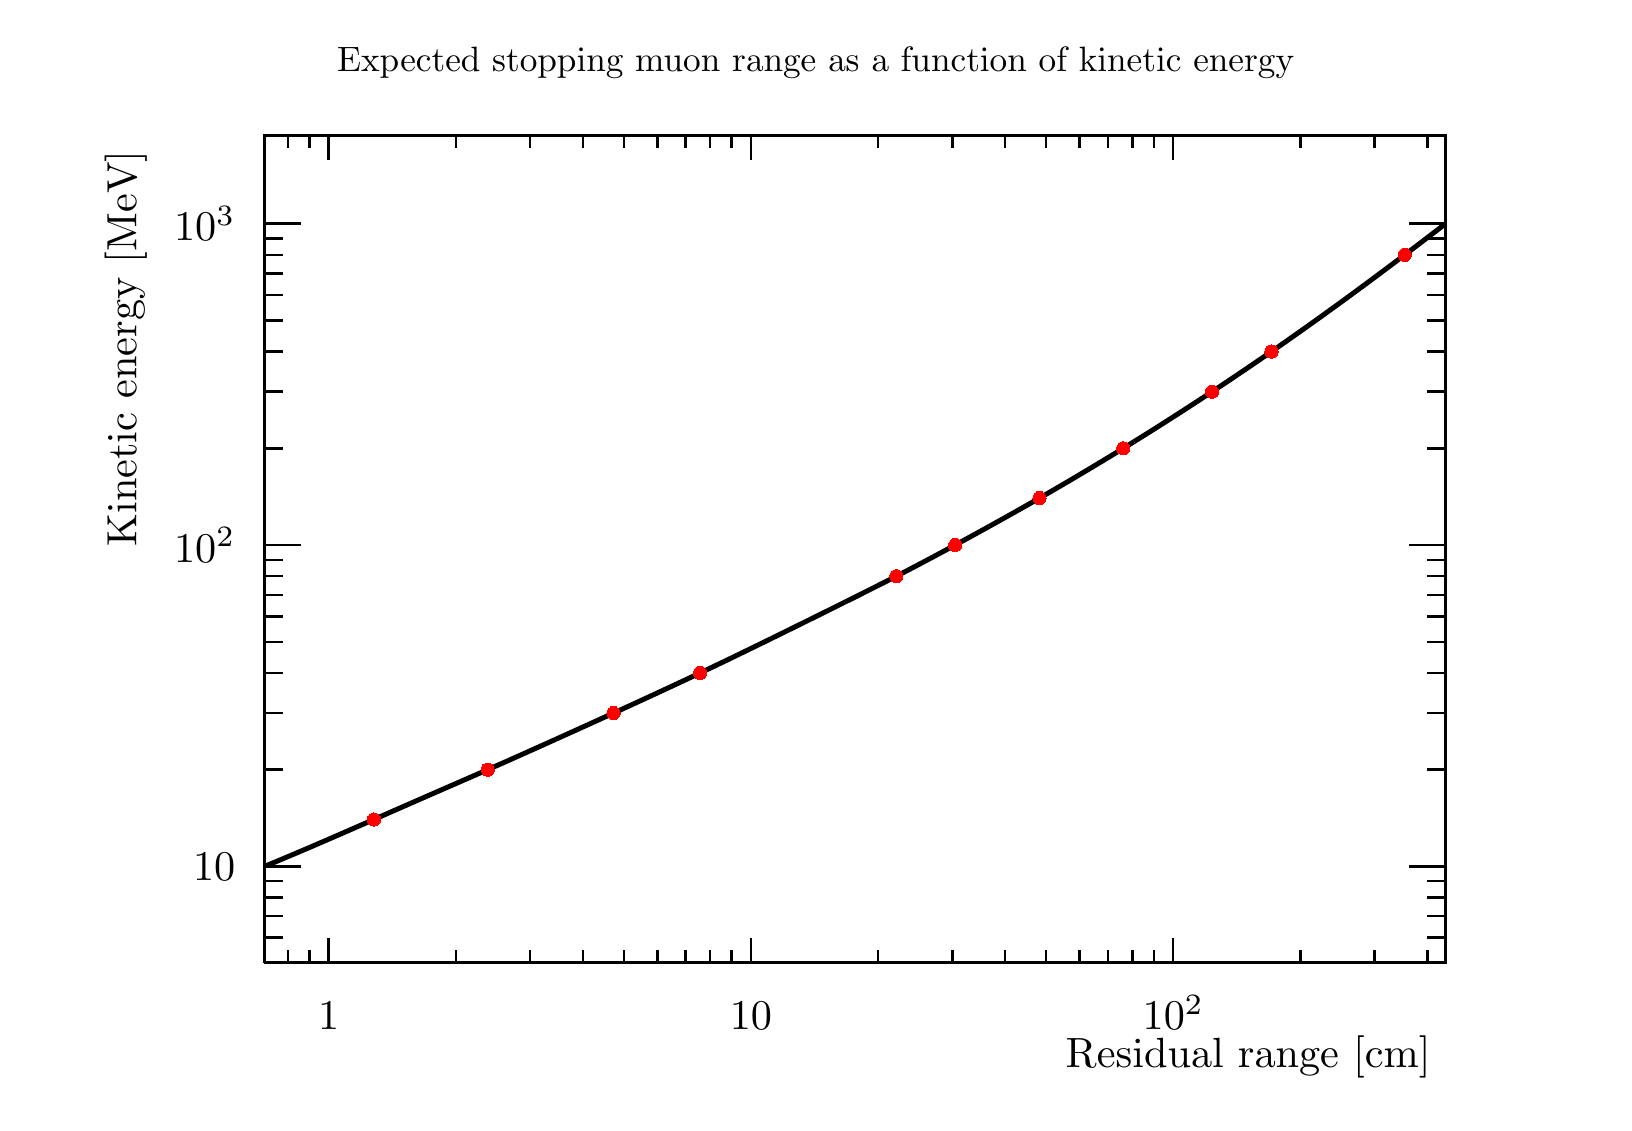
\begin{tikzpicture}
\pgfdeclareplotmark{cross} {
\pgfpathmoveto{\pgfpoint{-0.3\pgfplotmarksize}{\pgfplotmarksize}}
\pgfpathlineto{\pgfpoint{+0.3\pgfplotmarksize}{\pgfplotmarksize}}
\pgfpathlineto{\pgfpoint{+0.3\pgfplotmarksize}{0.3\pgfplotmarksize}}
\pgfpathlineto{\pgfpoint{+1\pgfplotmarksize}{0.3\pgfplotmarksize}}
\pgfpathlineto{\pgfpoint{+1\pgfplotmarksize}{-0.3\pgfplotmarksize}}
\pgfpathlineto{\pgfpoint{+0.3\pgfplotmarksize}{-0.3\pgfplotmarksize}}
\pgfpathlineto{\pgfpoint{+0.3\pgfplotmarksize}{-1.\pgfplotmarksize}}
\pgfpathlineto{\pgfpoint{-0.3\pgfplotmarksize}{-1.\pgfplotmarksize}}
\pgfpathlineto{\pgfpoint{-0.3\pgfplotmarksize}{-0.3\pgfplotmarksize}}
\pgfpathlineto{\pgfpoint{-1.\pgfplotmarksize}{-0.3\pgfplotmarksize}}
\pgfpathlineto{\pgfpoint{-1.\pgfplotmarksize}{0.3\pgfplotmarksize}}
\pgfpathlineto{\pgfpoint{-0.3\pgfplotmarksize}{0.3\pgfplotmarksize}}
\pgfpathclose
\pgfusepathqstroke
}
\pgfdeclareplotmark{cross*} {
\pgfpathmoveto{\pgfpoint{-0.3\pgfplotmarksize}{\pgfplotmarksize}}
\pgfpathlineto{\pgfpoint{+0.3\pgfplotmarksize}{\pgfplotmarksize}}
\pgfpathlineto{\pgfpoint{+0.3\pgfplotmarksize}{0.3\pgfplotmarksize}}
\pgfpathlineto{\pgfpoint{+1\pgfplotmarksize}{0.3\pgfplotmarksize}}
\pgfpathlineto{\pgfpoint{+1\pgfplotmarksize}{-0.3\pgfplotmarksize}}
\pgfpathlineto{\pgfpoint{+0.3\pgfplotmarksize}{-0.3\pgfplotmarksize}}
\pgfpathlineto{\pgfpoint{+0.3\pgfplotmarksize}{-1.\pgfplotmarksize}}
\pgfpathlineto{\pgfpoint{-0.3\pgfplotmarksize}{-1.\pgfplotmarksize}}
\pgfpathlineto{\pgfpoint{-0.3\pgfplotmarksize}{-0.3\pgfplotmarksize}}
\pgfpathlineto{\pgfpoint{-1.\pgfplotmarksize}{-0.3\pgfplotmarksize}}
\pgfpathlineto{\pgfpoint{-1.\pgfplotmarksize}{0.3\pgfplotmarksize}}
\pgfpathlineto{\pgfpoint{-0.3\pgfplotmarksize}{0.3\pgfplotmarksize}}
\pgfpathclose
\pgfusepathqfillstroke
}
\pgfdeclareplotmark{newstar} {
\pgfpathmoveto{\pgfqpoint{0pt}{\pgfplotmarksize}}
\pgfpathlineto{\pgfqpointpolar{44}{0.5\pgfplotmarksize}}
\pgfpathlineto{\pgfqpointpolar{18}{\pgfplotmarksize}}
\pgfpathlineto{\pgfqpointpolar{-20}{0.5\pgfplotmarksize}}
\pgfpathlineto{\pgfqpointpolar{-54}{\pgfplotmarksize}}
\pgfpathlineto{\pgfqpointpolar{-90}{0.5\pgfplotmarksize}}
\pgfpathlineto{\pgfqpointpolar{234}{\pgfplotmarksize}}
\pgfpathlineto{\pgfqpointpolar{198}{0.5\pgfplotmarksize}}
\pgfpathlineto{\pgfqpointpolar{162}{\pgfplotmarksize}}
\pgfpathlineto{\pgfqpointpolar{134}{0.5\pgfplotmarksize}}
\pgfpathclose
\pgfusepathqstroke
}
\pgfdeclareplotmark{newstar*} {
\pgfpathmoveto{\pgfqpoint{0pt}{\pgfplotmarksize}}
\pgfpathlineto{\pgfqpointpolar{44}{0.5\pgfplotmarksize}}
\pgfpathlineto{\pgfqpointpolar{18}{\pgfplotmarksize}}
\pgfpathlineto{\pgfqpointpolar{-20}{0.5\pgfplotmarksize}}
\pgfpathlineto{\pgfqpointpolar{-54}{\pgfplotmarksize}}
\pgfpathlineto{\pgfqpointpolar{-90}{0.5\pgfplotmarksize}}
\pgfpathlineto{\pgfqpointpolar{234}{\pgfplotmarksize}}
\pgfpathlineto{\pgfqpointpolar{198}{0.5\pgfplotmarksize}}
\pgfpathlineto{\pgfqpointpolar{162}{\pgfplotmarksize}}
\pgfpathlineto{\pgfqpointpolar{134}{0.5\pgfplotmarksize}}
\pgfpathclose
\pgfusepathqfillstroke
}
\definecolor{c}{rgb}{1,1,1};
\draw [color=c, fill=c] (0,0) rectangle (20,13.639);
\draw [color=c, fill=c] (3,1.77307) rectangle (18,12.2751);
\definecolor{c}{rgb}{0,0,0};
\draw [c,line width=0.9] (3,1.77307) -- (3,12.2751) -- (18,12.2751) -- (18,1.77307) -- (3,1.77307);
\definecolor{c}{rgb}{1,1,1};
\draw [color=c, fill=c] (0,0) rectangle (20,13.639);
\draw [color=c, fill=c] (3,1.77307) rectangle (18,12.2751);
\definecolor{c}{rgb}{0,0,0};
\draw [c,line width=0.9] (3,1.77307) -- (3,12.2751) -- (18,12.2751) -- (18,1.77307) -- (3,1.77307);
\draw [c,line width=1.8] (3.01883,3.00168) -- (3.05633,3.01716) -- (3.09383,3.03268) -- (3.13133,3.04826) -- (3.16883,3.06388) -- (3.20633,3.07955) -- (3.24383,3.09526) -- (3.28133,3.11102) -- (3.31883,3.12682) -- (3.35633,3.14266) --
 (3.39383,3.15854) -- (3.43133,3.17446) -- (3.46883,3.19042) -- (3.50633,3.20641) -- (3.54383,3.22244) -- (3.58133,3.2385) -- (3.61883,3.25459) -- (3.65633,3.27071) -- (3.69383,3.28686) -- (3.73133,3.30304) -- (3.76883,3.31925) -- (3.80633,3.33548)
 -- (3.84383,3.35173) -- (3.88133,3.36801) -- (3.91883,3.38431) -- (3.95633,3.40063) -- (3.99383,3.41696) -- (4.03133,3.43332) -- (4.06883,3.44968) -- (4.10633,3.46607) -- (4.14383,3.48246) -- (4.18133,3.49887) -- (4.21883,3.51529) --
 (4.25633,3.53172) -- (4.29383,3.54816) -- (4.33133,3.5646) -- (4.36883,3.58105) -- (4.40633,3.59751) -- (4.44383,3.61397) -- (4.48133,3.63043) -- (4.51883,3.64689) -- (4.55633,3.66335) -- (4.59383,3.67982) -- (4.63133,3.69628) -- (4.66883,3.71274)
 -- (4.70633,3.72919) -- (4.74383,3.74565) -- (4.78133,3.7621) -- (4.81883,3.77854) -- (4.85633,3.79498);
\draw [c,line width=1.8] (4.85633,3.79498) -- (4.89383,3.81141) -- (4.93133,3.82784) -- (4.96883,3.84426) -- (5.00633,3.86067) -- (5.04383,3.87707) -- (5.08133,3.89347) -- (5.11883,3.90986) -- (5.15633,3.92625) -- (5.19383,3.94262) -- (5.23133,3.959)
 -- (5.26883,3.97536) -- (5.30633,3.99172) -- (5.34383,4.00808) -- (5.38133,4.02444) -- (5.41883,4.04079) -- (5.45633,4.05714) -- (5.49383,4.0735) -- (5.53133,4.08985) -- (5.56883,4.10621) -- (5.60633,4.12258) -- (5.64383,4.13896) --
 (5.68133,4.15535) -- (5.71883,4.17176) -- (5.75633,4.18818) -- (5.79383,4.20463) -- (5.83133,4.2211) -- (5.86883,4.2376) -- (5.90633,4.25413) -- (5.94383,4.27069) -- (5.98133,4.28727) -- (6.01883,4.30388) -- (6.05633,4.32052) -- (6.09383,4.33717) --
 (6.13133,4.35385) -- (6.16883,4.37055) -- (6.20633,4.38728) -- (6.24383,4.40402) -- (6.28133,4.42077) -- (6.31883,4.43755) -- (6.35633,4.45434) -- (6.39383,4.47115) -- (6.43133,4.48797) -- (6.46883,4.50481) -- (6.50633,4.52165) -- (6.54383,4.53851)
 -- (6.58133,4.55538) -- (6.61883,4.57227) -- (6.65633,4.58916) -- (6.69383,4.60606);
\draw [c,line width=1.8] (6.69383,4.60606) -- (6.73133,4.62297) -- (6.76883,4.63989) -- (6.80633,4.65682) -- (6.84383,4.67375) -- (6.88133,4.6907) -- (6.91883,4.70765) -- (6.95633,4.72461) -- (6.99383,4.74157) -- (7.03133,4.75855) --
 (7.06883,4.77553) -- (7.10633,4.79252) -- (7.14383,4.80952) -- (7.18133,4.82653) -- (7.21883,4.84356) -- (7.25633,4.86059) -- (7.29383,4.87764) -- (7.33133,4.89469) -- (7.36883,4.91177) -- (7.40633,4.92886) -- (7.44383,4.94597) -- (7.48133,4.9631)
 -- (7.51883,4.98025) -- (7.55633,4.99741) -- (7.59383,5.0146) -- (7.63133,5.0318) -- (7.66883,5.04902) -- (7.70633,5.06626) -- (7.74383,5.08351) -- (7.78133,5.10078) -- (7.81883,5.11806) -- (7.85633,5.13537) -- (7.89383,5.15268) -- (7.93133,5.17002)
 -- (7.96883,5.18737) -- (8.00633,5.20474) -- (8.04383,5.22213) -- (8.08133,5.23954) -- (8.11883,5.25696) -- (8.15633,5.27441) -- (8.19383,5.29188) -- (8.23133,5.30936) -- (8.26883,5.32688) -- (8.30633,5.34442) -- (8.34383,5.36198) --
 (8.38133,5.37957) -- (8.41883,5.3972) -- (8.45633,5.41485) -- (8.49383,5.43254) -- (8.53133,5.45027);
\draw [c,line width=1.8] (8.53133,5.45027) -- (8.56883,5.46804) -- (8.60633,5.48585) -- (8.64383,5.50369) -- (8.68133,5.52157) -- (8.71883,5.53949) -- (8.75633,5.55744) -- (8.79383,5.57543) -- (8.83133,5.59345) -- (8.86883,5.6115) --
 (8.90633,5.62958) -- (8.94383,5.64769) -- (8.98133,5.66582) -- (9.01883,5.68399) -- (9.05633,5.70218) -- (9.09383,5.72039) -- (9.13133,5.73863) -- (9.16883,5.75689) -- (9.20633,5.77517) -- (9.24383,5.79348) -- (9.28133,5.8118) -- (9.31883,5.83014)
 -- (9.35633,5.8485) -- (9.39383,5.86688) -- (9.43133,5.88527) -- (9.46883,5.90368) -- (9.50633,5.9221) -- (9.54383,5.94054) -- (9.58133,5.95899) -- (9.61883,5.97745) -- (9.65633,5.99593) -- (9.69383,6.01441) -- (9.73133,6.03291) -- (9.76883,6.05142)
 -- (9.80633,6.06994) -- (9.84383,6.08846) -- (9.88133,6.107) -- (9.91883,6.12555) -- (9.95633,6.1441) -- (9.99383,6.16267) -- (10.0313,6.18124) -- (10.0688,6.19983) -- (10.1063,6.21842) -- (10.1438,6.23702) -- (10.1813,6.25564) -- (10.2188,6.27426)
 -- (10.2563,6.2929) -- (10.2938,6.31154) -- (10.3313,6.3302) -- (10.3688,6.34888);
\draw [c,line width=1.8] (10.3688,6.34888) -- (10.4063,6.36757) -- (10.4438,6.38628) -- (10.4813,6.405) -- (10.5188,6.42374) -- (10.5563,6.44251) -- (10.5938,6.4613) -- (10.6313,6.48011) -- (10.6688,6.49895) -- (10.7063,6.51782) -- (10.7438,6.53673)
 -- (10.7813,6.55567) -- (10.8188,6.57464) -- (10.8563,6.59366) -- (10.8938,6.61273) -- (10.9313,6.63185) -- (10.9688,6.65102) -- (11.0063,6.67025) -- (11.0438,6.68954) -- (11.0813,6.7089) -- (11.1188,6.72832) -- (11.1563,6.7478) -- (11.1938,6.76735)
 -- (11.2313,6.78695) -- (11.2688,6.80662) -- (11.3063,6.82634) -- (11.3438,6.84611) -- (11.3813,6.86594) -- (11.4188,6.88583) -- (11.4563,6.90577) -- (11.4938,6.92575) -- (11.5313,6.94579) -- (11.5688,6.96587) -- (11.6063,6.986) -- (11.6438,7.00617)
 -- (11.6813,7.02639) -- (11.7188,7.04665) -- (11.7563,7.06694) -- (11.7938,7.08728) -- (11.8313,7.10765) -- (11.8688,7.12806) -- (11.9063,7.14851) -- (11.9438,7.16899) -- (11.9813,7.18951) -- (12.0188,7.21006) -- (12.0563,7.23065) --
 (12.0938,7.25128) -- (12.1313,7.27194) -- (12.1688,7.29264) -- (12.2063,7.31338);
\draw [c,line width=1.8] (12.2063,7.31338) -- (12.2438,7.33416) -- (12.2813,7.35497) -- (12.3188,7.37582) -- (12.3563,7.39671) -- (12.3938,7.41764) -- (12.4313,7.4386) -- (12.4688,7.45961) -- (12.5063,7.48066) -- (12.5438,7.50176) --
 (12.5813,7.52289) -- (12.6188,7.54408) -- (12.6563,7.5653) -- (12.6938,7.58658) -- (12.7313,7.60791) -- (12.7688,7.62928) -- (12.8063,7.65071) -- (12.8438,7.67219) -- (12.8813,7.69374) -- (12.9188,7.71533) -- (12.9563,7.73698) -- (12.9938,7.75869)
 -- (13.0313,7.78046) -- (13.0688,7.80227) -- (13.1063,7.82415) -- (13.1438,7.84607) -- (13.1813,7.86806) -- (13.2188,7.89009) -- (13.2563,7.91218) -- (13.2938,7.93432) -- (13.3313,7.95652) -- (13.3688,7.97877) -- (13.4063,8.00107) --
 (13.4438,8.02342) -- (13.4813,8.04583) -- (13.5188,8.06829) -- (13.5563,8.09081) -- (13.5938,8.11338) -- (13.6313,8.136) -- (13.6688,8.15868) -- (13.7063,8.18141) -- (13.7438,8.20419) -- (13.7813,8.22704) -- (13.8188,8.24993) -- (13.8563,8.27289) --
 (13.8938,8.2959) -- (13.9313,8.31897) -- (13.9688,8.3421) -- (14.0063,8.36528) -- (14.0438,8.38852);
\draw [c,line width=1.8] (14.0438,8.38852) -- (14.0813,8.41182) -- (14.1188,8.43518) -- (14.1563,8.45859) -- (14.1938,8.48206) -- (14.2313,8.50558) -- (14.2688,8.52916) -- (14.3063,8.55279) -- (14.3438,8.57648) -- (14.3813,8.60023) --
 (14.4188,8.62403) -- (14.4563,8.64788) -- (14.4938,8.67179) -- (14.5313,8.69575) -- (14.5688,8.71977) -- (14.6063,8.74385) -- (14.6438,8.76797) -- (14.6813,8.79216) -- (14.7188,8.8164) -- (14.7563,8.84069) -- (14.7938,8.86504) -- (14.8313,8.88945)
 -- (14.8688,8.91391) -- (14.9063,8.93843) -- (14.9438,8.96301) -- (14.9813,8.98765) -- (15.0188,9.01234) -- (15.0563,9.03709) -- (15.0938,9.0619) -- (15.1313,9.08677) -- (15.1688,9.1117) -- (15.2063,9.13669) -- (15.2438,9.16174) -- (15.2813,9.18684)
 -- (15.3188,9.21201) -- (15.3563,9.23723) -- (15.3938,9.26252) -- (15.4313,9.28786) -- (15.4688,9.31326) -- (15.5063,9.33872) -- (15.5438,9.36424) -- (15.5813,9.38982) -- (15.6188,9.41546) -- (15.6563,9.44116) -- (15.6938,9.46692) --
 (15.7313,9.49275) -- (15.7688,9.51863) -- (15.8063,9.54458) -- (15.8438,9.57059) -- (15.8813,9.59666);
\draw [c,line width=1.8] (15.8813,9.59666) -- (15.9188,9.62279) -- (15.9563,9.64898) -- (15.9938,9.67524) -- (16.0313,9.70155) -- (16.0688,9.72792) -- (16.1063,9.75436) -- (16.1438,9.78085) -- (16.1813,9.8074) -- (16.2188,9.834) -- (16.2563,9.86067)
 -- (16.2938,9.88739) -- (16.3313,9.91416) -- (16.3688,9.941) -- (16.4063,9.96789) -- (16.4438,9.99483) -- (16.4813,10.0218) -- (16.5188,10.0489) -- (16.5563,10.076) -- (16.5938,10.1031) -- (16.6313,10.1304) -- (16.6688,10.1576) -- (16.7063,10.1849)
 -- (16.7438,10.2123) -- (16.7813,10.2397) -- (16.8188,10.2672) -- (16.8563,10.2947) -- (16.8938,10.3223) -- (16.9313,10.3499) -- (16.9688,10.3776) -- (17.0063,10.4053) -- (17.0438,10.4331) -- (17.0813,10.4609) -- (17.1188,10.4888) --
 (17.1563,10.5167) -- (17.1938,10.5447) -- (17.2313,10.5727) -- (17.2688,10.6008) -- (17.3063,10.6289) -- (17.3438,10.657) -- (17.3813,10.6852) -- (17.4188,10.7135) -- (17.4563,10.7418) -- (17.4938,10.7701) -- (17.5313,10.7985) -- (17.5688,10.8269)
 -- (17.6063,10.8554) -- (17.6438,10.8839) -- (17.6813,10.9124) -- (17.7188,10.941);
\draw [c,line width=1.8] (17.7188,10.941) -- (17.7563,10.9696) -- (17.7938,10.9983) -- (17.8313,11.027) -- (17.8688,11.0558) -- (17.9063,11.0846) -- (17.9438,11.1134) -- (17.9813,11.1423);
\draw [c,line width=0.9] (3,1.77307) -- (18,1.77307);
\draw [c,line width=0.9] (3.2965,1.9265) -- (3.2965,1.77307);
\draw [c,line width=0.9] (3.57082,1.9265) -- (3.57082,1.77307);
\draw [c,line width=0.9] (3.8162,2.07994) -- (3.8162,1.77307);
\draw [anchor=base] (3.8162,0.92063) node[scale=1.52731, color=c, rotate=0]{1};
\draw [c,line width=0.9] (5.43053,1.9265) -- (5.43053,1.77307);
\draw [c,line width=0.9] (6.37485,1.9265) -- (6.37485,1.77307);
\draw [c,line width=0.9] (7.04486,1.9265) -- (7.04486,1.77307);
\draw [c,line width=0.9] (7.56456,1.9265) -- (7.56456,1.77307);
\draw [c,line width=0.9] (7.98918,1.9265) -- (7.98918,1.77307);
\draw [c,line width=0.9] (8.34819,1.9265) -- (8.34819,1.77307);
\draw [c,line width=0.9] (8.65919,1.9265) -- (8.65919,1.77307);
\draw [c,line width=0.9] (8.9335,1.9265) -- (8.9335,1.77307);
\draw [c,line width=0.9] (9.17888,2.07994) -- (9.17888,1.77307);
\draw [anchor=base] (9.17888,0.92063) node[scale=1.52731, color=c, rotate=0]{10};
\draw [c,line width=0.9] (10.7932,1.9265) -- (10.7932,1.77307);
\draw [c,line width=0.9] (11.7375,1.9265) -- (11.7375,1.77307);
\draw [c,line width=0.9] (12.4075,1.9265) -- (12.4075,1.77307);
\draw [c,line width=0.9] (12.9272,1.9265) -- (12.9272,1.77307);
\draw [c,line width=0.9] (13.3519,1.9265) -- (13.3519,1.77307);
\draw [c,line width=0.9] (13.7109,1.9265) -- (13.7109,1.77307);
\draw [c,line width=0.9] (14.0219,1.9265) -- (14.0219,1.77307);
\draw [c,line width=0.9] (14.2962,1.9265) -- (14.2962,1.77307);
\draw [c,line width=0.9] (14.5416,2.07994) -- (14.5416,1.77307);
\draw [anchor=base] (14.5416,0.92063) node[scale=1.52731, color=c, rotate=0]{$10^{2}$};
\draw [c,line width=0.9] (16.1559,1.9265) -- (16.1559,1.77307);
\draw [c,line width=0.9] (17.1002,1.9265) -- (17.1002,1.77307);
\draw [c,line width=0.9] (17.7702,1.9265) -- (17.7702,1.77307);
\draw [anchor= east] (18,0.572837) node[scale=1.52731, color=c, rotate=0]{ Residual range [cm]};
\draw [c,line width=0.9] (3,12.2751) -- (18,12.2751);
\draw [c,line width=0.9] (3.2965,12.1216) -- (3.2965,12.2751);
\draw [c,line width=0.9] (3.57082,12.1216) -- (3.57082,12.2751);
\draw [c,line width=0.9] (3.8162,11.9682) -- (3.8162,12.2751);
\draw [c,line width=0.9] (5.43053,12.1216) -- (5.43053,12.2751);
\draw [c,line width=0.9] (6.37485,12.1216) -- (6.37485,12.2751);
\draw [c,line width=0.9] (7.04486,12.1216) -- (7.04486,12.2751);
\draw [c,line width=0.9] (7.56456,12.1216) -- (7.56456,12.2751);
\draw [c,line width=0.9] (7.98918,12.1216) -- (7.98918,12.2751);
\draw [c,line width=0.9] (8.34819,12.1216) -- (8.34819,12.2751);
\draw [c,line width=0.9] (8.65919,12.1216) -- (8.65919,12.2751);
\draw [c,line width=0.9] (8.9335,12.1216) -- (8.9335,12.2751);
\draw [c,line width=0.9] (9.17888,11.9682) -- (9.17888,12.2751);
\draw [c,line width=0.9] (10.7932,12.1216) -- (10.7932,12.2751);
\draw [c,line width=0.9] (11.7375,12.1216) -- (11.7375,12.2751);
\draw [c,line width=0.9] (12.4075,12.1216) -- (12.4075,12.2751);
\draw [c,line width=0.9] (12.9272,12.1216) -- (12.9272,12.2751);
\draw [c,line width=0.9] (13.3519,12.1216) -- (13.3519,12.2751);
\draw [c,line width=0.9] (13.7109,12.1216) -- (13.7109,12.2751);
\draw [c,line width=0.9] (14.0219,12.1216) -- (14.0219,12.2751);
\draw [c,line width=0.9] (14.2962,12.1216) -- (14.2962,12.2751);
\draw [c,line width=0.9] (14.5416,11.9682) -- (14.5416,12.2751);
\draw [c,line width=0.9] (16.1559,12.1216) -- (16.1559,12.2751);
\draw [c,line width=0.9] (17.1002,12.1216) -- (17.1002,12.2751);
\draw [c,line width=0.9] (17.7702,12.1216) -- (17.7702,12.2751);
\draw [c,line width=0.9] (3,1.77307) -- (3,12.2751);
\draw [c,line width=0.9] (3.231,2.08848) -- (3,2.08848);
\draw [c,line width=0.9] (3.231,2.36172) -- (3,2.36172);
\draw [c,line width=0.9] (3.231,2.5984) -- (3,2.5984);
\draw [c,line width=0.9] (3.231,2.80718) -- (3,2.80718);
\draw [c,line width=0.9] (3.462,2.99393) -- (3,2.99393);
\draw [anchor= east] (2.82,2.99393) node[scale=1.52731, color=c, rotate=0]{10};
\draw [c,line width=0.9] (3.231,4.22255) -- (3,4.22255);
\draw [c,line width=0.9] (3.231,4.94124) -- (3,4.94124);
\draw [c,line width=0.9] (3.231,5.45116) -- (3,5.45116);
\draw [c,line width=0.9] (3.231,5.84669) -- (3,5.84669);
\draw [c,line width=0.9] (3.231,6.16986) -- (3,6.16986);
\draw [c,line width=0.9] (3.231,6.44309) -- (3,6.44309);
\draw [c,line width=0.9] (3.231,6.67978) -- (3,6.67978);
\draw [c,line width=0.9] (3.231,6.88855) -- (3,6.88855);
\draw [c,line width=0.9] (3.462,7.07531) -- (3,7.07531);
\draw [anchor= east] (2.82,7.07531) node[scale=1.52731, color=c, rotate=0]{$10^{2}$};
\draw [c,line width=0.9] (3.231,8.30392) -- (3,8.30392);
\draw [c,line width=0.9] (3.231,9.02262) -- (3,9.02262);
\draw [c,line width=0.9] (3.231,9.53254) -- (3,9.53254);
\draw [c,line width=0.9] (3.231,9.92807) -- (3,9.92807);
\draw [c,line width=0.9] (3.231,10.2512) -- (3,10.2512);
\draw [c,line width=0.9] (3.231,10.5245) -- (3,10.5245);
\draw [c,line width=0.9] (3.231,10.7612) -- (3,10.7612);
\draw [c,line width=0.9] (3.231,10.9699) -- (3,10.9699);
\draw [c,line width=0.9] (3.462,11.1567) -- (3,11.1567);
\draw [anchor= east] (2.82,11.1567) node[scale=1.52731, color=c, rotate=0]{$10^{3}$};
\draw [anchor= east] (1.24,12.2751) node[scale=1.52731, color=c, rotate=90]{ Kinetic energy [MeV]};
\draw [c,line width=0.9] (18,1.77307) -- (18,12.2751);
\draw [c,line width=0.9] (17.769,2.08848) -- (18,2.08848);
\draw [c,line width=0.9] (17.769,2.36172) -- (18,2.36172);
\draw [c,line width=0.9] (17.769,2.5984) -- (18,2.5984);
\draw [c,line width=0.9] (17.769,2.80718) -- (18,2.80718);
\draw [c,line width=0.9] (17.538,2.99393) -- (18,2.99393);
\draw [c,line width=0.9] (17.769,4.22255) -- (18,4.22255);
\draw [c,line width=0.9] (17.769,4.94124) -- (18,4.94124);
\draw [c,line width=0.9] (17.769,5.45116) -- (18,5.45116);
\draw [c,line width=0.9] (17.769,5.84669) -- (18,5.84669);
\draw [c,line width=0.9] (17.769,6.16986) -- (18,6.16986);
\draw [c,line width=0.9] (17.769,6.44309) -- (18,6.44309);
\draw [c,line width=0.9] (17.769,6.67978) -- (18,6.67978);
\draw [c,line width=0.9] (17.769,6.88855) -- (18,6.88855);
\draw [c,line width=0.9] (17.538,7.07531) -- (18,7.07531);
\draw [c,line width=0.9] (17.769,8.30392) -- (18,8.30392);
\draw [c,line width=0.9] (17.769,9.02262) -- (18,9.02262);
\draw [c,line width=0.9] (17.769,9.53254) -- (18,9.53254);
\draw [c,line width=0.9] (17.769,9.92807) -- (18,9.92807);
\draw [c,line width=0.9] (17.769,10.2512) -- (18,10.2512);
\draw [c,line width=0.9] (17.769,10.5245) -- (18,10.5245);
\draw [c,line width=0.9] (17.769,10.7612) -- (18,10.7612);
\draw [c,line width=0.9] (17.769,10.9699) -- (18,10.9699);
\draw [c,line width=0.9] (17.538,11.1567) -- (18,11.1567);
\definecolor{c}{rgb}{1,0,0};
\foreach \P in {(4.38998,3.59034), (5.83462,4.22255), (7.43347,4.94124), (8.53322,5.45117), (11.0249,6.67978), (11.7718,7.07531), (12.843,7.67171), (13.9069,8.30392), (15.0344,9.02262), (15.7889,9.53254), (17.482,10.7612)}{\draw[mark
 options={color=c,fill=c},mark size=2.402402pt, line width=0.000000pt, mark=*] plot coordinates {\P};}
\definecolor{c}{rgb}{1,1,1};
\draw [color=c, fill=c] (2,12.8206) rectangle (18,13.5708);
\definecolor{c}{rgb}{0,0,0};
\draw (10,13.1957) node[scale=1.27276, color=c, rotate=0]{Expected stopping muon range as a function of kinetic energy};
\end{tikzpicture}

	\end{adjustbox}
	\caption[Muon range in liquid argon as a function of kinetic energy]{Muon range in liquid argon under the continuous slowing down approximation (CSDA) as a function of kinetic energy. The red points are taken from~\cite{muonCSDA}. The black line is a cubic spline drawn through the points.}
	\label{fig:keVsRange}
\end{figure}

%% Track selection
From \citefig{fig:muonEDep} left and right, one can see that, aside from the last 40 or \SI{50}{\cm} of the track, muons will have uniform energy deposition in liquid argon.
Therefore, any track selection used for detector calibration should avoid using the ends of muon tracks.
However, excluding the last \SI{50}{\cm} of all muon tracks regardless of if they stop in the detector or not would result in a significant volume of the detector which could not be effectively calibrated by this method.
Therefore, it is decided to instead select all those cosmic ray tracks which exit the detector and assume that they are not close to stopping.
Specifically, those tracks that cross the cathode and at least one of the anodes are selected.

Cathode-anode crossers are selected using cuts on the track start and end points. 
A track is considered to cross the cathode and an anode if one track end point is reconstructed with $X > \SI{340}{\cm}$ and the other is reconstructed with $X < \SI{0}{\cm}$.
Alternatively, if a track has one end point reconstructed with $X > \SI{0}{\cm}$ and the other end point is reconstructed with $X < \SI{-340}{\cm}$ it is considered to cross the cathode and the anode.

Requiring that tracks cross the cathode and an anode has two outcomes.
Firstly, it ensures that all the selected tracks have lengths equal to at least the drift distance and excludes short tracks that may be more easily mis-reconstructed.

Secondly, it allows the tracks to be given a definite time at which they entered the TPC.
As mentioned in \citesec{sec:dune:fd:lartpc}, TPCs such as ProtoDUNE-SP produce multiple 2-dimensional images which can be combined via reconstruction algorithms~\cite{pandora} to form 3-dimensional reconstructed tracks.
Typically, for neutrino induced events in LAr TPCs a definite drift coordinate can be reconstructed using timing information from the neutrino beam.

However for external particles such as cosmic rays, which are impinging on the detector continuously, this beam timing information is obviously not available.
Instead, reconstruction techniques must be utilised.

Specifically, the Pandora software package~\cite{pandora} looks at tracks in the two TPCs, separated by the central cathode.
If two 3-dimensional clusters in neighbouring drift volumes have similar direction vectors and an equal and opposite shift in the drift direction from the cathode, they can be stitched across the cathode to form one larger track.
This track will therefore have a definite time at which it crossed the cathode, often termed a $t_{0}$.
In turn, this allows definite drift coordinates and times to be reconstructed for all points in the track via the equation
\begin{equation}
	t_{\text{drift}} = t_{\text{hit}} - t_{0} \, ,
\end{equation}
where $t_{\text{hit}}$ is the recorded hit time in the TPC.

Cosmic rays are identified by the Pandora reconstruction chain. 
This reconstruction chain focusses on reconstructing track-like particle and has been shown to work well in the MicroBooNE experiment~\cite{pandoraUboone}. 
Tracks satisfying one of three conditions are considered to be produced by cosmic rays.
Firstly, those tracks starting at the top of the detector and ending at the bottom are considered to be cosmic rays.
Secondly, those tracks with a reconstructed $t_{0}$ which is inconsistent with the beam time are also considered to be cosmic rays.
Finally, any tracks which have reconstructed hits which appear to be outside the detector when assuming $t_0 = 0$ are considered to be inconsistent with beam particles and are thus cosmic rays.

%% Angular cuts explanation
Constraints are also placed on the angle of tracks used in the selection.
These constraints are in place due to difficulties in reconstructing the track \dqdx at certain angles.
This issue is shown in \citefigR{fig:dqdxAng}, which shows the average track \dqdx as a function of two angles, \thetai{XZ} and \thetai{YZ}.

These track angles are described respectively by the formulae
\begin{align}
	\thetai{XZ}	&= \arctan \left( \frac{\boldsymbol{X}}{\boldsymbol{Z}} \right) \\
	\thetai{YZ} &= \arctan \left( \frac{\boldsymbol{Y}}{\boldsymbol{Z}} \right) \, ,
\end{align}	
where $\boldsymbol{X}$, $\boldsymbol{Y}$ and $\boldsymbol{Z}$ are the direction vectors of the track.

One can see that at certain values of \thetai{XZ} (around $\pm\ang{90}$) and \thetai{yz} (around \ang{-90}) the average track \dqdx falls significantly.
The difference around $\thetai{XZ} = \pm \ang{90}$ is caused by tracks travelling close to parallel with the drift direction while the difference at $\thetai{YZ} = \ang{-90}$ is due to tracks travelling vertically downwards.
However, \citefigL{fig:dqdxAng} shows that this does have the effect of cutting out a large number of the tracks.

\begin{figure}[h]
	\begin{minipage}[t]{.5\linewidth}
		\begin{adjustbox}{max totalsize=\linewidth, center}
			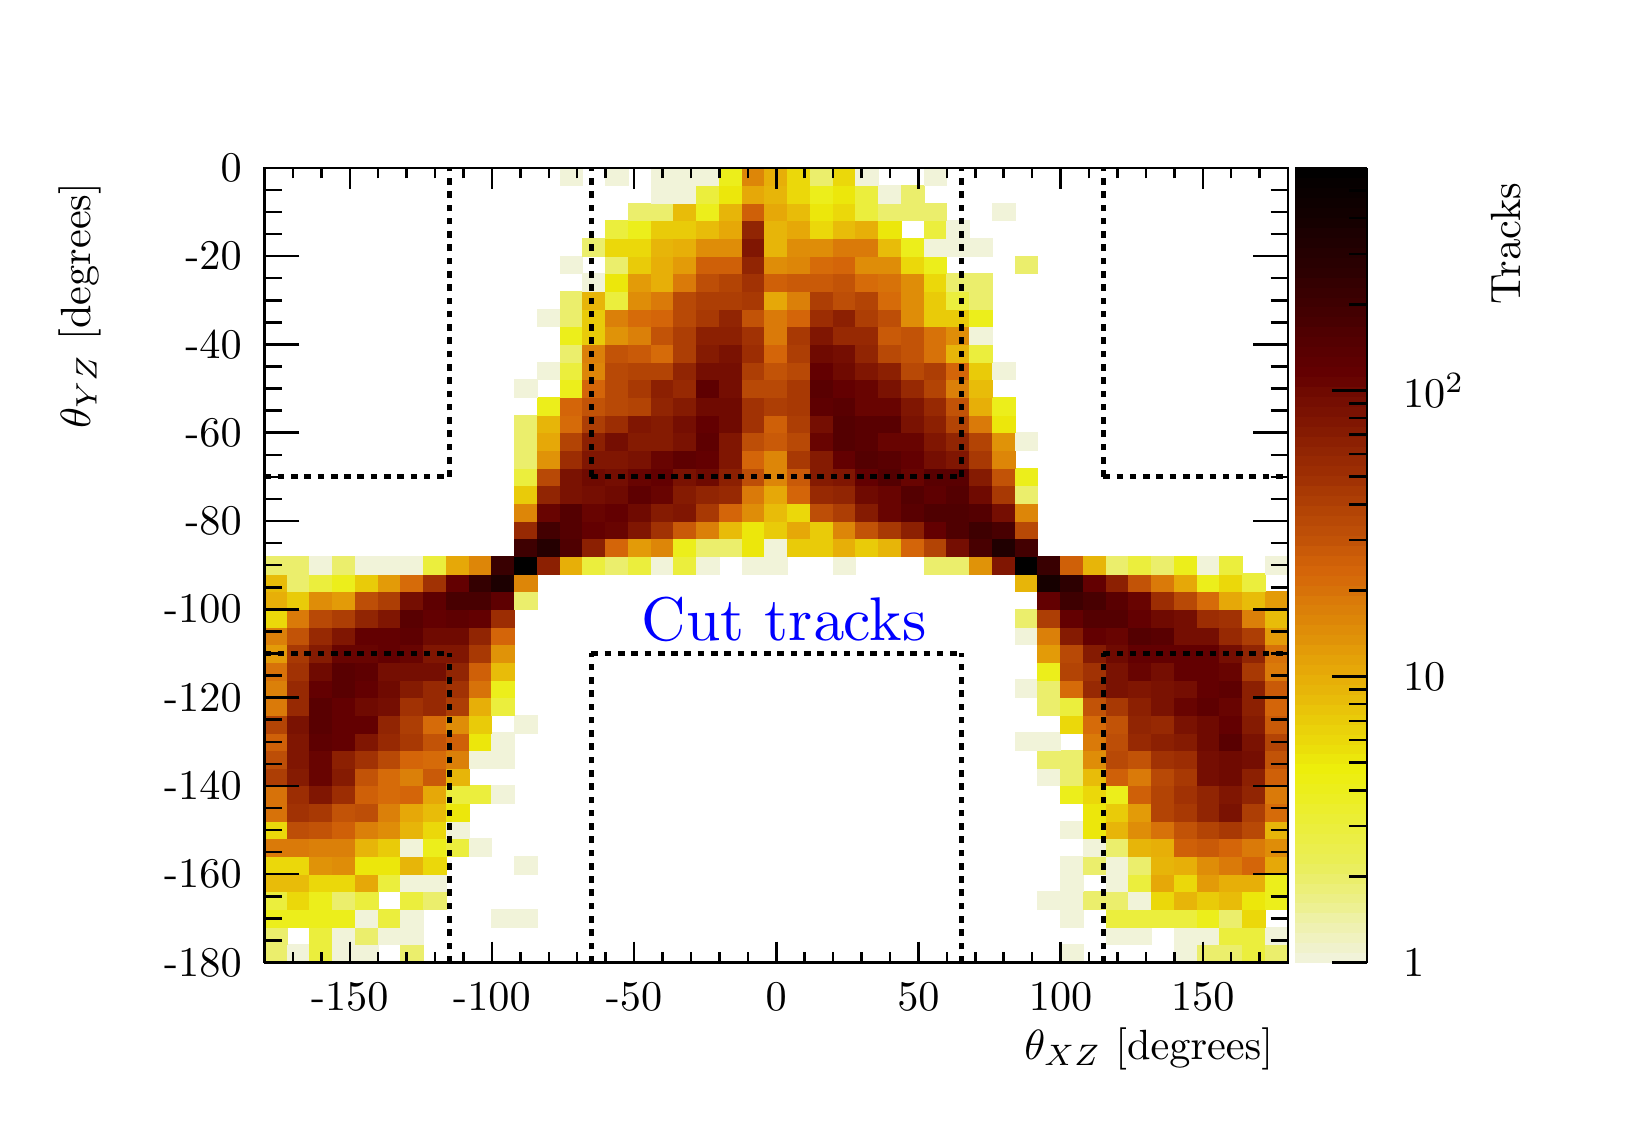
\begin{tikzpicture}
\pgfdeclareplotmark{cross} {
\pgfpathmoveto{\pgfpoint{-0.3\pgfplotmarksize}{\pgfplotmarksize}}
\pgfpathlineto{\pgfpoint{+0.3\pgfplotmarksize}{\pgfplotmarksize}}
\pgfpathlineto{\pgfpoint{+0.3\pgfplotmarksize}{0.3\pgfplotmarksize}}
\pgfpathlineto{\pgfpoint{+1\pgfplotmarksize}{0.3\pgfplotmarksize}}
\pgfpathlineto{\pgfpoint{+1\pgfplotmarksize}{-0.3\pgfplotmarksize}}
\pgfpathlineto{\pgfpoint{+0.3\pgfplotmarksize}{-0.3\pgfplotmarksize}}
\pgfpathlineto{\pgfpoint{+0.3\pgfplotmarksize}{-1.\pgfplotmarksize}}
\pgfpathlineto{\pgfpoint{-0.3\pgfplotmarksize}{-1.\pgfplotmarksize}}
\pgfpathlineto{\pgfpoint{-0.3\pgfplotmarksize}{-0.3\pgfplotmarksize}}
\pgfpathlineto{\pgfpoint{-1.\pgfplotmarksize}{-0.3\pgfplotmarksize}}
\pgfpathlineto{\pgfpoint{-1.\pgfplotmarksize}{0.3\pgfplotmarksize}}
\pgfpathlineto{\pgfpoint{-0.3\pgfplotmarksize}{0.3\pgfplotmarksize}}
\pgfpathclose
\pgfusepathqstroke
}
\pgfdeclareplotmark{cross*} {
\pgfpathmoveto{\pgfpoint{-0.3\pgfplotmarksize}{\pgfplotmarksize}}
\pgfpathlineto{\pgfpoint{+0.3\pgfplotmarksize}{\pgfplotmarksize}}
\pgfpathlineto{\pgfpoint{+0.3\pgfplotmarksize}{0.3\pgfplotmarksize}}
\pgfpathlineto{\pgfpoint{+1\pgfplotmarksize}{0.3\pgfplotmarksize}}
\pgfpathlineto{\pgfpoint{+1\pgfplotmarksize}{-0.3\pgfplotmarksize}}
\pgfpathlineto{\pgfpoint{+0.3\pgfplotmarksize}{-0.3\pgfplotmarksize}}
\pgfpathlineto{\pgfpoint{+0.3\pgfplotmarksize}{-1.\pgfplotmarksize}}
\pgfpathlineto{\pgfpoint{-0.3\pgfplotmarksize}{-1.\pgfplotmarksize}}
\pgfpathlineto{\pgfpoint{-0.3\pgfplotmarksize}{-0.3\pgfplotmarksize}}
\pgfpathlineto{\pgfpoint{-1.\pgfplotmarksize}{-0.3\pgfplotmarksize}}
\pgfpathlineto{\pgfpoint{-1.\pgfplotmarksize}{0.3\pgfplotmarksize}}
\pgfpathlineto{\pgfpoint{-0.3\pgfplotmarksize}{0.3\pgfplotmarksize}}
\pgfpathclose
\pgfusepathqfillstroke
}
\pgfdeclareplotmark{newstar} {
\pgfpathmoveto{\pgfqpoint{0pt}{\pgfplotmarksize}}
\pgfpathlineto{\pgfqpointpolar{44}{0.5\pgfplotmarksize}}
\pgfpathlineto{\pgfqpointpolar{18}{\pgfplotmarksize}}
\pgfpathlineto{\pgfqpointpolar{-20}{0.5\pgfplotmarksize}}
\pgfpathlineto{\pgfqpointpolar{-54}{\pgfplotmarksize}}
\pgfpathlineto{\pgfqpointpolar{-90}{0.5\pgfplotmarksize}}
\pgfpathlineto{\pgfqpointpolar{234}{\pgfplotmarksize}}
\pgfpathlineto{\pgfqpointpolar{198}{0.5\pgfplotmarksize}}
\pgfpathlineto{\pgfqpointpolar{162}{\pgfplotmarksize}}
\pgfpathlineto{\pgfqpointpolar{134}{0.5\pgfplotmarksize}}
\pgfpathclose
\pgfusepathqstroke
}
\pgfdeclareplotmark{newstar*} {
\pgfpathmoveto{\pgfqpoint{0pt}{\pgfplotmarksize}}
\pgfpathlineto{\pgfqpointpolar{44}{0.5\pgfplotmarksize}}
\pgfpathlineto{\pgfqpointpolar{18}{\pgfplotmarksize}}
\pgfpathlineto{\pgfqpointpolar{-20}{0.5\pgfplotmarksize}}
\pgfpathlineto{\pgfqpointpolar{-54}{\pgfplotmarksize}}
\pgfpathlineto{\pgfqpointpolar{-90}{0.5\pgfplotmarksize}}
\pgfpathlineto{\pgfqpointpolar{234}{\pgfplotmarksize}}
\pgfpathlineto{\pgfqpointpolar{198}{0.5\pgfplotmarksize}}
\pgfpathlineto{\pgfqpointpolar{162}{\pgfplotmarksize}}
\pgfpathlineto{\pgfqpointpolar{134}{0.5\pgfplotmarksize}}
\pgfpathclose
\pgfusepathqfillstroke
}
\definecolor{c}{rgb}{1,1,1};
\draw [color=c, fill=c] (0,0) rectangle (20,13.639);
\draw [color=c, fill=c] (3,1.77307) rectangle (16,11.8659);
\definecolor{c}{rgb}{0,0,0};
\draw [c,line width=0.9] (3,1.77307) -- (3,11.8659) -- (16,11.8659) -- (16,1.77307) -- (3,1.77307);
\definecolor{c}{rgb}{1,1,1};
\draw [color=c, fill=c] (3,1.77307) rectangle (16,11.8659);
\definecolor{c}{rgb}{0,0,0};
\draw [c,line width=0.9] (3,1.77307) -- (3,11.8659) -- (16,11.8659) -- (16,1.77307) -- (3,1.77307);
\definecolor{c}{rgb}{0.920683,0.935231,0.423782};
\draw [color=c, fill=c] (3,1.77307) rectangle (3.28889,1.99735);
\definecolor{c}{rgb}{0.945984,0.951044,0.850727};
\draw [color=c, fill=c] (3.28889,1.77307) rectangle (3.57778,1.99735);
\definecolor{c}{rgb}{0.922426,0.933333,0.238725};
\draw [color=c, fill=c] (3.57778,1.77307) rectangle (3.86667,1.99735);
\definecolor{c}{rgb}{0.945984,0.951044,0.850727};
\draw [color=c, fill=c] (3.86667,1.77307) rectangle (4.15556,1.99735);
\draw [color=c, fill=c] (4.15556,1.77307) rectangle (4.44444,1.99735);
\definecolor{c}{rgb}{0.920683,0.935231,0.423782};
\draw [color=c, fill=c] (4.73333,1.77307) rectangle (5.02222,1.99735);
\definecolor{c}{rgb}{0.945984,0.951044,0.850727};
\draw [color=c, fill=c] (13.1111,1.77307) rectangle (13.4,1.99735);
\draw [color=c, fill=c] (14.5556,1.77307) rectangle (14.8444,1.99735);
\definecolor{c}{rgb}{0.920683,0.935231,0.423782};
\draw [color=c, fill=c] (14.8444,1.77307) rectangle (15.1333,1.99735);
\draw [color=c, fill=c] (15.1333,1.77307) rectangle (15.4222,1.99735);
\definecolor{c}{rgb}{0.922426,0.933333,0.238725};
\draw [color=c, fill=c] (15.4222,1.77307) rectangle (15.7111,1.99735);
\definecolor{c}{rgb}{0.920683,0.935231,0.423782};
\draw [color=c, fill=c] (15.7111,1.77307) rectangle (16,1.99735);
\draw [color=c, fill=c] (3,1.99735) rectangle (3.28889,2.22164);
\definecolor{c}{rgb}{0.922426,0.933333,0.238725};
\draw [color=c, fill=c] (3.57778,1.99735) rectangle (3.86667,2.22164);
\definecolor{c}{rgb}{0.945984,0.951044,0.850727};
\draw [color=c, fill=c] (3.86667,1.99735) rectangle (4.15556,2.22164);
\definecolor{c}{rgb}{0.920683,0.935231,0.423782};
\draw [color=c, fill=c] (4.15556,1.99735) rectangle (4.44444,2.22164);
\definecolor{c}{rgb}{0.945984,0.951044,0.850727};
\draw [color=c, fill=c] (4.44444,1.99735) rectangle (4.73333,2.22164);
\draw [color=c, fill=c] (4.73333,1.99735) rectangle (5.02222,2.22164);
\draw [color=c, fill=c] (13.6889,1.99735) rectangle (13.9778,2.22164);
\draw [color=c, fill=c] (13.9778,1.99735) rectangle (14.2667,2.22164);
\draw [color=c, fill=c] (14.5556,1.99735) rectangle (14.8444,2.22164);
\draw [color=c, fill=c] (14.8444,1.99735) rectangle (15.1333,2.22164);
\definecolor{c}{rgb}{0.922426,0.933333,0.238725};
\draw [color=c, fill=c] (15.1333,1.99735) rectangle (15.4222,2.22164);
\draw [color=c, fill=c] (15.4222,1.99735) rectangle (15.7111,2.22164);
\definecolor{c}{rgb}{0.945984,0.951044,0.850727};
\draw [color=c, fill=c] (15.7111,1.99735) rectangle (16,2.22164);
\definecolor{c}{rgb}{0.927206,0.933333,0.104902};
\draw [color=c, fill=c] (3,2.22164) rectangle (3.28889,2.44592);
\draw [color=c, fill=c] (3.28889,2.22164) rectangle (3.57778,2.44592);
\draw [color=c, fill=c] (3.57778,2.22164) rectangle (3.86667,2.44592);
\draw [color=c, fill=c] (3.86667,2.22164) rectangle (4.15556,2.44592);
\definecolor{c}{rgb}{0.945984,0.951044,0.850727};
\draw [color=c, fill=c] (4.15556,2.22164) rectangle (4.44444,2.44592);
\definecolor{c}{rgb}{0.922426,0.933333,0.238725};
\draw [color=c, fill=c] (4.44444,2.22164) rectangle (4.73333,2.44592);
\definecolor{c}{rgb}{0.945984,0.951044,0.850727};
\draw [color=c, fill=c] (4.73333,2.22164) rectangle (5.02222,2.44592);
\draw [color=c, fill=c] (5.88889,2.22164) rectangle (6.17778,2.44592);
\draw [color=c, fill=c] (6.17778,2.22164) rectangle (6.46667,2.44592);
\draw [color=c, fill=c] (13.1111,2.22164) rectangle (13.4,2.44592);
\definecolor{c}{rgb}{0.922426,0.933333,0.238725};
\draw [color=c, fill=c] (13.6889,2.22164) rectangle (13.9778,2.44592);
\draw [color=c, fill=c] (13.9778,2.22164) rectangle (14.2667,2.44592);
\draw [color=c, fill=c] (14.2667,2.22164) rectangle (14.5556,2.44592);
\draw [color=c, fill=c] (14.5556,2.22164) rectangle (14.8444,2.44592);
\definecolor{c}{rgb}{0.927206,0.933333,0.104902};
\draw [color=c, fill=c] (14.8444,2.22164) rectangle (15.1333,2.44592);
\definecolor{c}{rgb}{0.920683,0.935231,0.423782};
\draw [color=c, fill=c] (15.1333,2.22164) rectangle (15.4222,2.44592);
\definecolor{c}{rgb}{0.920833,0.847549,0.0394608};
\draw [color=c, fill=c] (15.4222,2.22164) rectangle (15.7111,2.44592);
\definecolor{c}{rgb}{0.922426,0.933333,0.238725};
\draw [color=c, fill=c] (3,2.44592) rectangle (3.28889,2.67021);
\definecolor{c}{rgb}{0.920833,0.847549,0.0394608};
\draw [color=c, fill=c] (3.28889,2.44592) rectangle (3.57778,2.67021);
\definecolor{c}{rgb}{0.927206,0.933333,0.104902};
\draw [color=c, fill=c] (3.57778,2.44592) rectangle (3.86667,2.67021);
\definecolor{c}{rgb}{0.920683,0.935231,0.423782};
\draw [color=c, fill=c] (3.86667,2.44592) rectangle (4.15556,2.67021);
\definecolor{c}{rgb}{0.922426,0.933333,0.238725};
\draw [color=c, fill=c] (4.15556,2.44592) rectangle (4.44444,2.67021);
\draw [color=c, fill=c] (4.73333,2.44592) rectangle (5.02222,2.67021);
\definecolor{c}{rgb}{0.920683,0.935231,0.423782};
\draw [color=c, fill=c] (5.02222,2.44592) rectangle (5.31111,2.67021);
\definecolor{c}{rgb}{0.945984,0.951044,0.850727};
\draw [color=c, fill=c] (12.8222,2.44592) rectangle (13.1111,2.67021);
\draw [color=c, fill=c] (13.1111,2.44592) rectangle (13.4,2.67021);
\definecolor{c}{rgb}{0.920683,0.935231,0.423782};
\draw [color=c, fill=c] (13.4,2.44592) rectangle (13.6889,2.67021);
\draw [color=c, fill=c] (13.6889,2.44592) rectangle (13.9778,2.67021);
\definecolor{c}{rgb}{0.945984,0.951044,0.850727};
\draw [color=c, fill=c] (13.9778,2.44592) rectangle (14.2667,2.67021);
\definecolor{c}{rgb}{0.920833,0.847549,0.0394608};
\draw [color=c, fill=c] (14.2667,2.44592) rectangle (14.5556,2.67021);
\definecolor{c}{rgb}{0.907108,0.710294,0.0335784};
\draw [color=c, fill=c] (14.5556,2.44592) rectangle (14.8444,2.67021);
\definecolor{c}{rgb}{0.915686,0.796078,0.0372549};
\draw [color=c, fill=c] (14.8444,2.44592) rectangle (15.1333,2.67021);
\definecolor{c}{rgb}{0.909681,0.736029,0.0346814};
\draw [color=c, fill=c] (15.1333,2.44592) rectangle (15.4222,2.67021);
\definecolor{c}{rgb}{0.926838,0.907598,0.0420343};
\draw [color=c, fill=c] (15.4222,2.44592) rectangle (15.7111,2.67021);
\definecolor{c}{rgb}{0.927206,0.933333,0.104902};
\draw [color=c, fill=c] (15.7111,2.44592) rectangle (16,2.67021);
\definecolor{c}{rgb}{0.909681,0.736029,0.0346814};
\draw [color=c, fill=c] (3,2.67021) rectangle (3.28889,2.89449);
\draw [color=c, fill=c] (3.28889,2.67021) rectangle (3.57778,2.89449);
\definecolor{c}{rgb}{0.920833,0.847549,0.0394608};
\draw [color=c, fill=c] (3.57778,2.67021) rectangle (3.86667,2.89449);
\draw [color=c, fill=c] (3.86667,2.67021) rectangle (4.15556,2.89449);
\definecolor{c}{rgb}{0.901961,0.658824,0.0313726};
\draw [color=c, fill=c] (4.15556,2.67021) rectangle (4.44444,2.89449);
\definecolor{c}{rgb}{0.922426,0.933333,0.238725};
\draw [color=c, fill=c] (4.44444,2.67021) rectangle (4.73333,2.89449);
\definecolor{c}{rgb}{0.945984,0.951044,0.850727};
\draw [color=c, fill=c] (4.73333,2.67021) rectangle (5.02222,2.89449);
\draw [color=c, fill=c] (5.02222,2.67021) rectangle (5.31111,2.89449);
\draw [color=c, fill=c] (13.1111,2.67021) rectangle (13.4,2.89449);
\draw [color=c, fill=c] (13.6889,2.67021) rectangle (13.9778,2.89449);
\definecolor{c}{rgb}{0.922426,0.933333,0.238725};
\draw [color=c, fill=c] (13.9778,2.67021) rectangle (14.2667,2.89449);
\definecolor{c}{rgb}{0.901961,0.658824,0.0313726};
\draw [color=c, fill=c] (14.2667,2.67021) rectangle (14.5556,2.89449);
\definecolor{c}{rgb}{0.920833,0.847549,0.0394608};
\draw [color=c, fill=c] (14.5556,2.67021) rectangle (14.8444,2.89449);
\definecolor{c}{rgb}{0.888726,0.609559,0.0321078};
\draw [color=c, fill=c] (14.8444,2.67021) rectangle (15.1333,2.89449);
\definecolor{c}{rgb}{0.904534,0.684559,0.0324755};
\draw [color=c, fill=c] (15.1333,2.67021) rectangle (15.4222,2.89449);
\draw [color=c, fill=c] (15.4222,2.67021) rectangle (15.7111,2.89449);
\definecolor{c}{rgb}{0.927206,0.933333,0.104902};
\draw [color=c, fill=c] (15.7111,2.67021) rectangle (16,2.89449);
\definecolor{c}{rgb}{0.920833,0.847549,0.0394608};
\draw [color=c, fill=c] (3,2.89449) rectangle (3.28889,3.11878);
\draw [color=c, fill=c] (3.28889,2.89449) rectangle (3.57778,3.11878);
\definecolor{c}{rgb}{0.879902,0.576716,0.032598};
\draw [color=c, fill=c] (3.57778,2.89449) rectangle (3.86667,3.11878);
\definecolor{c}{rgb}{0.873284,0.552083,0.0329657};
\draw [color=c, fill=c] (3.86667,2.89449) rectangle (4.15556,3.11878);
\definecolor{c}{rgb}{0.926838,0.907598,0.0420343};
\draw [color=c, fill=c] (4.15556,2.89449) rectangle (4.44444,3.11878);
\draw [color=c, fill=c] (4.44444,2.89449) rectangle (4.73333,3.11878);
\definecolor{c}{rgb}{0.907108,0.710294,0.0335784};
\draw [color=c, fill=c] (4.73333,2.89449) rectangle (5.02222,3.11878);
\definecolor{c}{rgb}{0.920833,0.847549,0.0394608};
\draw [color=c, fill=c] (5.02222,2.89449) rectangle (5.31111,3.11878);
\definecolor{c}{rgb}{0.945984,0.951044,0.850727};
\draw [color=c, fill=c] (6.17778,2.89449) rectangle (6.46667,3.11878);
\draw [color=c, fill=c] (13.1111,2.89449) rectangle (13.4,3.11878);
\definecolor{c}{rgb}{0.920683,0.935231,0.423782};
\draw [color=c, fill=c] (13.4,2.89449) rectangle (13.6889,3.11878);
\definecolor{c}{rgb}{0.945984,0.951044,0.850727};
\draw [color=c, fill=c] (13.6889,2.89449) rectangle (13.9778,3.11878);
\definecolor{c}{rgb}{0.920683,0.935231,0.423782};
\draw [color=c, fill=c] (13.9778,2.89449) rectangle (14.2667,3.11878);
\definecolor{c}{rgb}{0.907108,0.710294,0.0335784};
\draw [color=c, fill=c] (14.2667,2.89449) rectangle (14.5556,3.11878);
\definecolor{c}{rgb}{0.904534,0.684559,0.0324755};
\draw [color=c, fill=c] (14.5556,2.89449) rectangle (14.8444,3.11878);
\definecolor{c}{rgb}{0.873284,0.552083,0.0329657};
\draw [color=c, fill=c] (14.8444,2.89449) rectangle (15.1333,3.11878);
\definecolor{c}{rgb}{0.853431,0.478186,0.0340686};
\draw [color=c, fill=c] (15.1333,2.89449) rectangle (15.4222,3.11878);
\definecolor{c}{rgb}{0.831373,0.396078,0.0352941};
\draw [color=c, fill=c] (15.4222,2.89449) rectangle (15.7111,3.11878);
\definecolor{c}{rgb}{0.901961,0.658824,0.0313726};
\draw [color=c, fill=c] (15.7111,2.89449) rectangle (16,3.11878);
\definecolor{c}{rgb}{0.853431,0.478186,0.0340686};
\draw [color=c, fill=c] (3,3.11878) rectangle (3.28889,3.34306);
\draw [color=c, fill=c] (3.28889,3.11878) rectangle (3.57778,3.34306);
\definecolor{c}{rgb}{0.860049,0.502819,0.033701};
\draw [color=c, fill=c] (3.57778,3.11878) rectangle (3.86667,3.34306);
\draw [color=c, fill=c] (3.86667,3.11878) rectangle (4.15556,3.34306);
\definecolor{c}{rgb}{0.907108,0.710294,0.0335784};
\draw [color=c, fill=c] (4.15556,3.11878) rectangle (4.44444,3.34306);
\definecolor{c}{rgb}{0.915686,0.796078,0.0372549};
\draw [color=c, fill=c] (4.44444,3.11878) rectangle (4.73333,3.34306);
\definecolor{c}{rgb}{0.945984,0.951044,0.850727};
\draw [color=c, fill=c] (4.73333,3.11878) rectangle (5.02222,3.34306);
\definecolor{c}{rgb}{0.927206,0.933333,0.104902};
\draw [color=c, fill=c] (5.02222,3.11878) rectangle (5.31111,3.34306);
\definecolor{c}{rgb}{0.922426,0.933333,0.238725};
\draw [color=c, fill=c] (5.31111,3.11878) rectangle (5.6,3.34306);
\definecolor{c}{rgb}{0.945984,0.951044,0.850727};
\draw [color=c, fill=c] (5.6,3.11878) rectangle (5.88889,3.34306);
\draw [color=c, fill=c] (13.4,3.11878) rectangle (13.6889,3.34306);
\definecolor{c}{rgb}{0.920683,0.935231,0.423782};
\draw [color=c, fill=c] (13.6889,3.11878) rectangle (13.9778,3.34306);
\definecolor{c}{rgb}{0.907108,0.710294,0.0335784};
\draw [color=c, fill=c] (13.9778,3.11878) rectangle (14.2667,3.34306);
\definecolor{c}{rgb}{0.904534,0.684559,0.0324755};
\draw [color=c, fill=c] (14.2667,3.11878) rectangle (14.5556,3.34306);
\definecolor{c}{rgb}{0.810784,0.37549,0.0330882};
\draw [color=c, fill=c] (14.5556,3.11878) rectangle (14.8444,3.34306);
\definecolor{c}{rgb}{0.790196,0.354902,0.0308824};
\draw [color=c, fill=c] (14.8444,3.11878) rectangle (15.1333,3.34306);
\definecolor{c}{rgb}{0.831373,0.396078,0.0352941};
\draw [color=c, fill=c] (15.1333,3.11878) rectangle (15.4222,3.34306);
\definecolor{c}{rgb}{0.853431,0.478186,0.0340686};
\draw [color=c, fill=c] (15.4222,3.11878) rectangle (15.7111,3.34306);
\definecolor{c}{rgb}{0.873284,0.552083,0.0329657};
\draw [color=c, fill=c] (15.7111,3.11878) rectangle (16,3.34306);
\definecolor{c}{rgb}{0.920833,0.847549,0.0394608};
\draw [color=c, fill=c] (3,3.34306) rectangle (3.28889,3.56735);
\definecolor{c}{rgb}{0.742157,0.306863,0.0257353};
\draw [color=c, fill=c] (3.28889,3.34306) rectangle (3.57778,3.56735);
\definecolor{c}{rgb}{0.762745,0.327451,0.0279412};
\draw [color=c, fill=c] (3.57778,3.34306) rectangle (3.86667,3.56735);
\definecolor{c}{rgb}{0.810784,0.37549,0.0330882};
\draw [color=c, fill=c] (3.86667,3.34306) rectangle (4.15556,3.56735);
\definecolor{c}{rgb}{0.860049,0.502819,0.033701};
\draw [color=c, fill=c] (4.15556,3.34306) rectangle (4.44444,3.56735);
\definecolor{c}{rgb}{0.873284,0.552083,0.0329657};
\draw [color=c, fill=c] (4.44444,3.34306) rectangle (4.73333,3.56735);
\definecolor{c}{rgb}{0.907108,0.710294,0.0335784};
\draw [color=c, fill=c] (4.73333,3.34306) rectangle (5.02222,3.56735);
\definecolor{c}{rgb}{0.920833,0.847549,0.0394608};
\draw [color=c, fill=c] (5.02222,3.34306) rectangle (5.31111,3.56735);
\definecolor{c}{rgb}{0.945984,0.951044,0.850727};
\draw [color=c, fill=c] (5.31111,3.34306) rectangle (5.6,3.56735);
\draw [color=c, fill=c] (13.1111,3.34306) rectangle (13.4,3.56735);
\definecolor{c}{rgb}{0.926838,0.907598,0.0420343};
\draw [color=c, fill=c] (13.4,3.34306) rectangle (13.6889,3.56735);
\definecolor{c}{rgb}{0.907108,0.710294,0.0335784};
\draw [color=c, fill=c] (13.6889,3.34306) rectangle (13.9778,3.56735);
\definecolor{c}{rgb}{0.873284,0.552083,0.0329657};
\draw [color=c, fill=c] (13.9778,3.34306) rectangle (14.2667,3.56735);
\definecolor{c}{rgb}{0.844608,0.445343,0.0345588};
\draw [color=c, fill=c] (14.2667,3.34306) rectangle (14.5556,3.56735);
\definecolor{c}{rgb}{0.762745,0.327451,0.0279412};
\draw [color=c, fill=c] (14.5556,3.34306) rectangle (14.8444,3.56735);
\definecolor{c}{rgb}{0.70098,0.265686,0.0213235};
\draw [color=c, fill=c] (14.8444,3.34306) rectangle (15.1333,3.56735);
\definecolor{c}{rgb}{0.659804,0.22451,0.0169118};
\draw [color=c, fill=c] (15.1333,3.34306) rectangle (15.4222,3.56735);
\definecolor{c}{rgb}{0.721569,0.286275,0.0235294};
\draw [color=c, fill=c] (15.4222,3.34306) rectangle (15.7111,3.56735);
\definecolor{c}{rgb}{0.907108,0.710294,0.0335784};
\draw [color=c, fill=c] (15.7111,3.34306) rectangle (16,3.56735);
\definecolor{c}{rgb}{0.844608,0.445343,0.0345588};
\draw [color=c, fill=c] (3,3.56735) rectangle (3.28889,3.79163);
\definecolor{c}{rgb}{0.632353,0.197059,0.0139706};
\draw [color=c, fill=c] (3.28889,3.56735) rectangle (3.57778,3.79163);
\definecolor{c}{rgb}{0.659804,0.22451,0.0169118};
\draw [color=c, fill=c] (3.57778,3.56735) rectangle (3.86667,3.79163);
\definecolor{c}{rgb}{0.762745,0.327451,0.0279412};
\draw [color=c, fill=c] (3.86667,3.56735) rectangle (4.15556,3.79163);
\definecolor{c}{rgb}{0.742157,0.306863,0.0257353};
\draw [color=c, fill=c] (4.15556,3.56735) rectangle (4.44444,3.79163);
\definecolor{c}{rgb}{0.860049,0.502819,0.033701};
\draw [color=c, fill=c] (4.44444,3.56735) rectangle (4.73333,3.79163);
\definecolor{c}{rgb}{0.901961,0.658824,0.0313726};
\draw [color=c, fill=c] (4.73333,3.56735) rectangle (5.02222,3.79163);
\definecolor{c}{rgb}{0.909681,0.736029,0.0346814};
\draw [color=c, fill=c] (5.02222,3.56735) rectangle (5.31111,3.79163);
\definecolor{c}{rgb}{0.926838,0.907598,0.0420343};
\draw [color=c, fill=c] (5.31111,3.56735) rectangle (5.6,3.79163);
\draw [color=c, fill=c] (13.4,3.56735) rectangle (13.6889,3.79163);
\definecolor{c}{rgb}{0.915686,0.796078,0.0372549};
\draw [color=c, fill=c] (13.6889,3.56735) rectangle (13.9778,3.79163);
\definecolor{c}{rgb}{0.888726,0.609559,0.0321078};
\draw [color=c, fill=c] (13.9778,3.56735) rectangle (14.2667,3.79163);
\definecolor{c}{rgb}{0.70098,0.265686,0.0213235};
\draw [color=c, fill=c] (14.2667,3.56735) rectangle (14.5556,3.79163);
\definecolor{c}{rgb}{0.659804,0.22451,0.0169118};
\draw [color=c, fill=c] (14.5556,3.56735) rectangle (14.8444,3.79163);
\definecolor{c}{rgb}{0.569853,0.143382,0.0102941};
\draw [color=c, fill=c] (14.8444,3.56735) rectangle (15.1333,3.79163);
\definecolor{c}{rgb}{0.479044,0.0716912,0.00710784};
\draw [color=c, fill=c] (15.1333,3.56735) rectangle (15.4222,3.79163);
\definecolor{c}{rgb}{0.680392,0.245098,0.0191176};
\draw [color=c, fill=c] (15.4222,3.56735) rectangle (15.7111,3.79163);
\definecolor{c}{rgb}{0.83799,0.420711,0.0349265};
\draw [color=c, fill=c] (15.7111,3.56735) rectangle (16,3.79163);
\definecolor{c}{rgb}{0.844608,0.445343,0.0345588};
\draw [color=c, fill=c] (3,3.79163) rectangle (3.28889,4.01592);
\definecolor{c}{rgb}{0.611765,0.176471,0.0117647};
\draw [color=c, fill=c] (3.28889,3.79163) rectangle (3.57778,4.01592);
\definecolor{c}{rgb}{0.5,0.0882353,0.00784314};
\draw [color=c, fill=c] (3.57778,3.79163) rectangle (3.86667,4.01592);
\definecolor{c}{rgb}{0.611765,0.176471,0.0117647};
\draw [color=c, fill=c] (3.86667,3.79163) rectangle (4.15556,4.01592);
\definecolor{c}{rgb}{0.810784,0.37549,0.0330882};
\draw [color=c, fill=c] (4.15556,3.79163) rectangle (4.44444,4.01592);
\definecolor{c}{rgb}{0.83799,0.420711,0.0349265};
\draw [color=c, fill=c] (4.44444,3.79163) rectangle (4.73333,4.01592);
\definecolor{c}{rgb}{0.831373,0.396078,0.0352941};
\draw [color=c, fill=c] (4.73333,3.79163) rectangle (5.02222,4.01592);
\definecolor{c}{rgb}{0.901961,0.658824,0.0313726};
\draw [color=c, fill=c] (5.02222,3.79163) rectangle (5.31111,4.01592);
\definecolor{c}{rgb}{0.922426,0.933333,0.238725};
\draw [color=c, fill=c] (5.31111,3.79163) rectangle (5.6,4.01592);
\draw [color=c, fill=c] (5.6,3.79163) rectangle (5.88889,4.01592);
\definecolor{c}{rgb}{0.945984,0.951044,0.850727};
\draw [color=c, fill=c] (5.88889,3.79163) rectangle (6.17778,4.01592);
\definecolor{c}{rgb}{0.927206,0.933333,0.104902};
\draw [color=c, fill=c] (13.1111,3.79163) rectangle (13.4,4.01592);
\definecolor{c}{rgb}{0.920833,0.847549,0.0394608};
\draw [color=c, fill=c] (13.4,3.79163) rectangle (13.6889,4.01592);
\definecolor{c}{rgb}{0.927206,0.933333,0.104902};
\draw [color=c, fill=c] (13.6889,3.79163) rectangle (13.9778,4.01592);
\definecolor{c}{rgb}{0.810784,0.37549,0.0330882};
\draw [color=c, fill=c] (13.9778,3.79163) rectangle (14.2667,4.01592);
\definecolor{c}{rgb}{0.70098,0.265686,0.0213235};
\draw [color=c, fill=c] (14.2667,3.79163) rectangle (14.5556,4.01592);
\definecolor{c}{rgb}{0.632353,0.197059,0.0139706};
\draw [color=c, fill=c] (14.5556,3.79163) rectangle (14.8444,4.01592);
\definecolor{c}{rgb}{0.569853,0.143382,0.0102941};
\draw [color=c, fill=c] (14.8444,3.79163) rectangle (15.1333,4.01592);
\definecolor{c}{rgb}{0.5,0.0882353,0.00784314};
\draw [color=c, fill=c] (15.1333,3.79163) rectangle (15.4222,4.01592);
\definecolor{c}{rgb}{0.569853,0.143382,0.0102941};
\draw [color=c, fill=c] (15.4222,3.79163) rectangle (15.7111,4.01592);
\definecolor{c}{rgb}{0.853431,0.478186,0.0340686};
\draw [color=c, fill=c] (15.7111,3.79163) rectangle (16,4.01592);
\definecolor{c}{rgb}{0.680392,0.245098,0.0191176};
\draw [color=c, fill=c] (3,4.01592) rectangle (3.28889,4.2402);
\definecolor{c}{rgb}{0.520956,0.104779,0.00857843};
\draw [color=c, fill=c] (3.28889,4.01592) rectangle (3.57778,4.2402);
\definecolor{c}{rgb}{0.409191,0.0165441,0.00465686};
\draw [color=c, fill=c] (3.57778,4.01592) rectangle (3.86667,4.2402);
\definecolor{c}{rgb}{0.520956,0.104779,0.00857843};
\draw [color=c, fill=c] (3.86667,4.01592) rectangle (4.15556,4.2402);
\definecolor{c}{rgb}{0.762745,0.327451,0.0279412};
\draw [color=c, fill=c] (4.15556,4.01592) rectangle (4.44444,4.2402);
\definecolor{c}{rgb}{0.83799,0.420711,0.0349265};
\draw [color=c, fill=c] (4.44444,4.01592) rectangle (4.73333,4.2402);
\definecolor{c}{rgb}{0.860049,0.502819,0.033701};
\draw [color=c, fill=c] (4.73333,4.01592) rectangle (5.02222,4.2402);
\definecolor{c}{rgb}{0.790196,0.354902,0.0308824};
\draw [color=c, fill=c] (5.02222,4.01592) rectangle (5.31111,4.2402);
\definecolor{c}{rgb}{0.907108,0.710294,0.0335784};
\draw [color=c, fill=c] (5.31111,4.01592) rectangle (5.6,4.2402);
\definecolor{c}{rgb}{0.945984,0.951044,0.850727};
\draw [color=c, fill=c] (12.8222,4.01592) rectangle (13.1111,4.2402);
\definecolor{c}{rgb}{0.920683,0.935231,0.423782};
\draw [color=c, fill=c] (13.1111,4.01592) rectangle (13.4,4.2402);
\definecolor{c}{rgb}{0.909681,0.736029,0.0346814};
\draw [color=c, fill=c] (13.4,4.01592) rectangle (13.6889,4.2402);
\definecolor{c}{rgb}{0.810784,0.37549,0.0330882};
\draw [color=c, fill=c] (13.6889,4.01592) rectangle (13.9778,4.2402);
\definecolor{c}{rgb}{0.853431,0.478186,0.0340686};
\draw [color=c, fill=c] (13.9778,4.01592) rectangle (14.2667,4.2402);
\definecolor{c}{rgb}{0.721569,0.286275,0.0235294};
\draw [color=c, fill=c] (14.2667,4.01592) rectangle (14.5556,4.2402);
\definecolor{c}{rgb}{0.659804,0.22451,0.0169118};
\draw [color=c, fill=c] (14.5556,4.01592) rectangle (14.8444,4.2402);
\definecolor{c}{rgb}{0.458088,0.0551471,0.00637255};
\draw [color=c, fill=c] (14.8444,4.01592) rectangle (15.1333,4.2402);
\definecolor{c}{rgb}{0.437132,0.0386029,0.00563726};
\draw [color=c, fill=c] (15.1333,4.01592) rectangle (15.4222,4.2402);
\definecolor{c}{rgb}{0.548897,0.126838,0.00955882};
\draw [color=c, fill=c] (15.4222,4.01592) rectangle (15.7111,4.2402);
\definecolor{c}{rgb}{0.810784,0.37549,0.0330882};
\draw [color=c, fill=c] (15.7111,4.01592) rectangle (16,4.2402);
\definecolor{c}{rgb}{0.742157,0.306863,0.0257353};
\draw [color=c, fill=c] (3,4.2402) rectangle (3.28889,4.46449);
\definecolor{c}{rgb}{0.5,0.0882353,0.00784314};
\draw [color=c, fill=c] (3.28889,4.2402) rectangle (3.57778,4.46449);
\definecolor{c}{rgb}{0.409191,0.0165441,0.00465686};
\draw [color=c, fill=c] (3.57778,4.2402) rectangle (3.86667,4.46449);
\definecolor{c}{rgb}{0.548897,0.126838,0.00955882};
\draw [color=c, fill=c] (3.86667,4.2402) rectangle (4.15556,4.46449);
\definecolor{c}{rgb}{0.632353,0.197059,0.0139706};
\draw [color=c, fill=c] (4.15556,4.2402) rectangle (4.44444,4.46449);
\definecolor{c}{rgb}{0.721569,0.286275,0.0235294};
\draw [color=c, fill=c] (4.44444,4.2402) rectangle (4.73333,4.46449);
\definecolor{c}{rgb}{0.831373,0.396078,0.0352941};
\draw [color=c, fill=c] (4.73333,4.2402) rectangle (5.02222,4.46449);
\definecolor{c}{rgb}{0.83799,0.420711,0.0349265};
\draw [color=c, fill=c] (5.02222,4.2402) rectangle (5.31111,4.46449);
\definecolor{c}{rgb}{0.860049,0.502819,0.033701};
\draw [color=c, fill=c] (5.31111,4.2402) rectangle (5.6,4.46449);
\definecolor{c}{rgb}{0.945984,0.951044,0.850727};
\draw [color=c, fill=c] (5.6,4.2402) rectangle (5.88889,4.46449);
\draw [color=c, fill=c] (5.88889,4.2402) rectangle (6.17778,4.46449);
\definecolor{c}{rgb}{0.920683,0.935231,0.423782};
\draw [color=c, fill=c] (12.8222,4.2402) rectangle (13.1111,4.46449);
\draw [color=c, fill=c] (13.1111,4.2402) rectangle (13.4,4.46449);
\definecolor{c}{rgb}{0.873284,0.552083,0.0329657};
\draw [color=c, fill=c] (13.4,4.2402) rectangle (13.6889,4.46449);
\definecolor{c}{rgb}{0.721569,0.286275,0.0235294};
\draw [color=c, fill=c] (13.6889,4.2402) rectangle (13.9778,4.46449);
\definecolor{c}{rgb}{0.762745,0.327451,0.0279412};
\draw [color=c, fill=c] (13.9778,4.2402) rectangle (14.2667,4.46449);
\definecolor{c}{rgb}{0.632353,0.197059,0.0139706};
\draw [color=c, fill=c] (14.2667,4.2402) rectangle (14.5556,4.46449);
\definecolor{c}{rgb}{0.611765,0.176471,0.0117647};
\draw [color=c, fill=c] (14.5556,4.2402) rectangle (14.8444,4.46449);
\definecolor{c}{rgb}{0.458088,0.0551471,0.00637255};
\draw [color=c, fill=c] (14.8444,4.2402) rectangle (15.1333,4.46449);
\definecolor{c}{rgb}{0.437132,0.0386029,0.00563726};
\draw [color=c, fill=c] (15.1333,4.2402) rectangle (15.4222,4.46449);
\definecolor{c}{rgb}{0.458088,0.0551471,0.00637255};
\draw [color=c, fill=c] (15.4222,4.2402) rectangle (15.7111,4.46449);
\definecolor{c}{rgb}{0.762745,0.327451,0.0279412};
\draw [color=c, fill=c] (15.7111,4.2402) rectangle (16,4.46449);
\definecolor{c}{rgb}{0.810784,0.37549,0.0330882};
\draw [color=c, fill=c] (3,4.46449) rectangle (3.28889,4.68877);
\definecolor{c}{rgb}{0.5,0.0882353,0.00784314};
\draw [color=c, fill=c] (3.28889,4.46449) rectangle (3.57778,4.68877);
\definecolor{c}{rgb}{0.368382,0,0.00392157};
\draw [color=c, fill=c] (3.57778,4.46449) rectangle (3.86667,4.68877);
\definecolor{c}{rgb}{0.388235,0,0.00392157};
\draw [color=c, fill=c] (3.86667,4.46449) rectangle (4.15556,4.68877);
\definecolor{c}{rgb}{0.5,0.0882353,0.00784314};
\draw [color=c, fill=c] (4.15556,4.46449) rectangle (4.44444,4.68877);
\definecolor{c}{rgb}{0.590809,0.159926,0.0110294};
\draw [color=c, fill=c] (4.44444,4.46449) rectangle (4.73333,4.68877);
\definecolor{c}{rgb}{0.659804,0.22451,0.0169118};
\draw [color=c, fill=c] (4.73333,4.46449) rectangle (5.02222,4.68877);
\definecolor{c}{rgb}{0.762745,0.327451,0.0279412};
\draw [color=c, fill=c] (5.02222,4.46449) rectangle (5.31111,4.68877);
\definecolor{c}{rgb}{0.810784,0.37549,0.0330882};
\draw [color=c, fill=c] (5.31111,4.46449) rectangle (5.6,4.68877);
\definecolor{c}{rgb}{0.926838,0.907598,0.0420343};
\draw [color=c, fill=c] (5.6,4.46449) rectangle (5.88889,4.68877);
\definecolor{c}{rgb}{0.945984,0.951044,0.850727};
\draw [color=c, fill=c] (5.88889,4.46449) rectangle (6.17778,4.68877);
\draw [color=c, fill=c] (12.5333,4.46449) rectangle (12.8222,4.68877);
\draw [color=c, fill=c] (12.8222,4.46449) rectangle (13.1111,4.68877);
\definecolor{c}{rgb}{0.853431,0.478186,0.0340686};
\draw [color=c, fill=c] (13.4,4.46449) rectangle (13.6889,4.68877);
\definecolor{c}{rgb}{0.742157,0.306863,0.0257353};
\draw [color=c, fill=c] (13.6889,4.46449) rectangle (13.9778,4.68877);
\definecolor{c}{rgb}{0.590809,0.159926,0.0110294};
\draw [color=c, fill=c] (13.9778,4.46449) rectangle (14.2667,4.68877);
\definecolor{c}{rgb}{0.548897,0.126838,0.00955882};
\draw [color=c, fill=c] (14.2667,4.46449) rectangle (14.5556,4.68877);
\definecolor{c}{rgb}{0.520956,0.104779,0.00857843};
\draw [color=c, fill=c] (14.5556,4.46449) rectangle (14.8444,4.68877);
\definecolor{c}{rgb}{0.437132,0.0386029,0.00563726};
\draw [color=c, fill=c] (14.8444,4.46449) rectangle (15.1333,4.68877);
\definecolor{c}{rgb}{0.348529,0,0.00392157};
\draw [color=c, fill=c] (15.1333,4.46449) rectangle (15.4222,4.68877);
\definecolor{c}{rgb}{0.479044,0.0716912,0.00710784};
\draw [color=c, fill=c] (15.4222,4.46449) rectangle (15.7111,4.68877);
\definecolor{c}{rgb}{0.70098,0.265686,0.0213235};
\draw [color=c, fill=c] (15.7111,4.46449) rectangle (16,4.68877);
\draw [color=c, fill=c] (3,4.68877) rectangle (3.28889,4.91306);
\definecolor{c}{rgb}{0.479044,0.0716912,0.00710784};
\draw [color=c, fill=c] (3.28889,4.68877) rectangle (3.57778,4.91306);
\definecolor{c}{rgb}{0.348529,0,0.00392157};
\draw [color=c, fill=c] (3.57778,4.68877) rectangle (3.86667,4.91306);
\definecolor{c}{rgb}{0.388235,0,0.00392157};
\draw [color=c, fill=c] (3.86667,4.68877) rectangle (4.15556,4.91306);
\draw [color=c, fill=c] (4.15556,4.68877) rectangle (4.44444,4.91306);
\definecolor{c}{rgb}{0.569853,0.143382,0.0102941};
\draw [color=c, fill=c] (4.44444,4.68877) rectangle (4.73333,4.91306);
\definecolor{c}{rgb}{0.680392,0.245098,0.0191176};
\draw [color=c, fill=c] (4.73333,4.68877) rectangle (5.02222,4.91306);
\definecolor{c}{rgb}{0.83799,0.420711,0.0349265};
\draw [color=c, fill=c] (5.02222,4.68877) rectangle (5.31111,4.91306);
\definecolor{c}{rgb}{0.873284,0.552083,0.0329657};
\draw [color=c, fill=c] (5.31111,4.68877) rectangle (5.6,4.91306);
\definecolor{c}{rgb}{0.915686,0.796078,0.0372549};
\draw [color=c, fill=c] (5.6,4.68877) rectangle (5.88889,4.91306);
\definecolor{c}{rgb}{0.945984,0.951044,0.850727};
\draw [color=c, fill=c] (6.17778,4.68877) rectangle (6.46667,4.91306);
\definecolor{c}{rgb}{0.920833,0.847549,0.0394608};
\draw [color=c, fill=c] (13.1111,4.68877) rectangle (13.4,4.91306);
\definecolor{c}{rgb}{0.83799,0.420711,0.0349265};
\draw [color=c, fill=c] (13.4,4.68877) rectangle (13.6889,4.91306);
\definecolor{c}{rgb}{0.762745,0.327451,0.0279412};
\draw [color=c, fill=c] (13.6889,4.68877) rectangle (13.9778,4.91306);
\definecolor{c}{rgb}{0.569853,0.143382,0.0102941};
\draw [color=c, fill=c] (13.9778,4.68877) rectangle (14.2667,4.91306);
\definecolor{c}{rgb}{0.590809,0.159926,0.0110294};
\draw [color=c, fill=c] (14.2667,4.68877) rectangle (14.5556,4.91306);
\definecolor{c}{rgb}{0.479044,0.0716912,0.00710784};
\draw [color=c, fill=c] (14.5556,4.68877) rectangle (14.8444,4.91306);
\definecolor{c}{rgb}{0.437132,0.0386029,0.00563726};
\draw [color=c, fill=c] (14.8444,4.68877) rectangle (15.1333,4.91306);
\definecolor{c}{rgb}{0.388235,0,0.00392157};
\draw [color=c, fill=c] (15.1333,4.68877) rectangle (15.4222,4.91306);
\definecolor{c}{rgb}{0.520956,0.104779,0.00857843};
\draw [color=c, fill=c] (15.4222,4.68877) rectangle (15.7111,4.91306);
\definecolor{c}{rgb}{0.790196,0.354902,0.0308824};
\draw [color=c, fill=c] (15.7111,4.68877) rectangle (16,4.91306);
\definecolor{c}{rgb}{0.853431,0.478186,0.0340686};
\draw [color=c, fill=c] (3,4.91306) rectangle (3.28889,5.13734);
\definecolor{c}{rgb}{0.590809,0.159926,0.0110294};
\draw [color=c, fill=c] (3.28889,4.91306) rectangle (3.57778,5.13734);
\definecolor{c}{rgb}{0.348529,0,0.00392157};
\draw [color=c, fill=c] (3.57778,4.91306) rectangle (3.86667,5.13734);
\definecolor{c}{rgb}{0.388235,0,0.00392157};
\draw [color=c, fill=c] (3.86667,4.91306) rectangle (4.15556,5.13734);
\definecolor{c}{rgb}{0.437132,0.0386029,0.00563726};
\draw [color=c, fill=c] (4.15556,4.91306) rectangle (4.44444,5.13734);
\definecolor{c}{rgb}{0.458088,0.0551471,0.00637255};
\draw [color=c, fill=c] (4.44444,4.91306) rectangle (4.73333,5.13734);
\definecolor{c}{rgb}{0.632353,0.197059,0.0139706};
\draw [color=c, fill=c] (4.73333,4.91306) rectangle (5.02222,5.13734);
\definecolor{c}{rgb}{0.590809,0.159926,0.0110294};
\draw [color=c, fill=c] (5.02222,4.91306) rectangle (5.31111,5.13734);
\definecolor{c}{rgb}{0.680392,0.245098,0.0191176};
\draw [color=c, fill=c] (5.31111,4.91306) rectangle (5.6,5.13734);
\definecolor{c}{rgb}{0.904534,0.684559,0.0324755};
\draw [color=c, fill=c] (5.6,4.91306) rectangle (5.88889,5.13734);
\definecolor{c}{rgb}{0.922426,0.933333,0.238725};
\draw [color=c, fill=c] (5.88889,4.91306) rectangle (6.17778,5.13734);
\definecolor{c}{rgb}{0.920683,0.935231,0.423782};
\draw [color=c, fill=c] (12.8222,4.91306) rectangle (13.1111,5.13734);
\definecolor{c}{rgb}{0.922426,0.933333,0.238725};
\draw [color=c, fill=c] (13.1111,4.91306) rectangle (13.4,5.13734);
\definecolor{c}{rgb}{0.762745,0.327451,0.0279412};
\draw [color=c, fill=c] (13.4,4.91306) rectangle (13.6889,5.13734);
\definecolor{c}{rgb}{0.659804,0.22451,0.0169118};
\draw [color=c, fill=c] (13.6889,4.91306) rectangle (13.9778,5.13734);
\definecolor{c}{rgb}{0.548897,0.126838,0.00955882};
\draw [color=c, fill=c] (13.9778,4.91306) rectangle (14.2667,5.13734);
\definecolor{c}{rgb}{0.479044,0.0716912,0.00710784};
\draw [color=c, fill=c] (14.2667,4.91306) rectangle (14.5556,5.13734);
\definecolor{c}{rgb}{0.409191,0.0165441,0.00465686};
\draw [color=c, fill=c] (14.5556,4.91306) rectangle (14.8444,5.13734);
\definecolor{c}{rgb}{0.368382,0,0.00392157};
\draw [color=c, fill=c] (14.8444,4.91306) rectangle (15.1333,5.13734);
\definecolor{c}{rgb}{0.409191,0.0165441,0.00465686};
\draw [color=c, fill=c] (15.1333,4.91306) rectangle (15.4222,5.13734);
\definecolor{c}{rgb}{0.548897,0.126838,0.00955882};
\draw [color=c, fill=c] (15.4222,4.91306) rectangle (15.7111,5.13734);
\definecolor{c}{rgb}{0.831373,0.396078,0.0352941};
\draw [color=c, fill=c] (15.7111,4.91306) rectangle (16,5.13734);
\definecolor{c}{rgb}{0.860049,0.502819,0.033701};
\draw [color=c, fill=c] (3,5.13734) rectangle (3.28889,5.36163);
\definecolor{c}{rgb}{0.590809,0.159926,0.0110294};
\draw [color=c, fill=c] (3.28889,5.13734) rectangle (3.57778,5.36163);
\definecolor{c}{rgb}{0.388235,0,0.00392157};
\draw [color=c, fill=c] (3.57778,5.13734) rectangle (3.86667,5.36163);
\definecolor{c}{rgb}{0.348529,0,0.00392157};
\draw [color=c, fill=c] (3.86667,5.13734) rectangle (4.15556,5.36163);
\definecolor{c}{rgb}{0.388235,0,0.00392157};
\draw [color=c, fill=c] (4.15556,5.13734) rectangle (4.44444,5.36163);
\definecolor{c}{rgb}{0.437132,0.0386029,0.00563726};
\draw [color=c, fill=c] (4.44444,5.13734) rectangle (4.73333,5.36163);
\definecolor{c}{rgb}{0.520956,0.104779,0.00857843};
\draw [color=c, fill=c] (4.73333,5.13734) rectangle (5.02222,5.36163);
\definecolor{c}{rgb}{0.590809,0.159926,0.0110294};
\draw [color=c, fill=c] (5.02222,5.13734) rectangle (5.31111,5.36163);
\definecolor{c}{rgb}{0.632353,0.197059,0.0139706};
\draw [color=c, fill=c] (5.31111,5.13734) rectangle (5.6,5.36163);
\definecolor{c}{rgb}{0.844608,0.445343,0.0345588};
\draw [color=c, fill=c] (5.6,5.13734) rectangle (5.88889,5.36163);
\definecolor{c}{rgb}{0.927206,0.933333,0.104902};
\draw [color=c, fill=c] (5.88889,5.13734) rectangle (6.17778,5.36163);
\definecolor{c}{rgb}{0.945984,0.951044,0.850727};
\draw [color=c, fill=c] (12.5333,5.13734) rectangle (12.8222,5.36163);
\definecolor{c}{rgb}{0.920683,0.935231,0.423782};
\draw [color=c, fill=c] (12.8222,5.13734) rectangle (13.1111,5.36163);
\definecolor{c}{rgb}{0.83799,0.420711,0.0349265};
\draw [color=c, fill=c] (13.1111,5.13734) rectangle (13.4,5.36163);
\definecolor{c}{rgb}{0.590809,0.159926,0.0110294};
\draw [color=c, fill=c] (13.4,5.13734) rectangle (13.6889,5.36163);
\definecolor{c}{rgb}{0.479044,0.0716912,0.00710784};
\draw [color=c, fill=c] (13.6889,5.13734) rectangle (13.9778,5.36163);
\definecolor{c}{rgb}{0.5,0.0882353,0.00784314};
\draw [color=c, fill=c] (13.9778,5.13734) rectangle (14.2667,5.36163);
\definecolor{c}{rgb}{0.479044,0.0716912,0.00710784};
\draw [color=c, fill=c] (14.2667,5.13734) rectangle (14.5556,5.36163);
\definecolor{c}{rgb}{0.458088,0.0551471,0.00637255};
\draw [color=c, fill=c] (14.5556,5.13734) rectangle (14.8444,5.36163);
\definecolor{c}{rgb}{0.388235,0,0.00392157};
\draw [color=c, fill=c] (14.8444,5.13734) rectangle (15.1333,5.36163);
\definecolor{c}{rgb}{0.368382,0,0.00392157};
\draw [color=c, fill=c] (15.1333,5.13734) rectangle (15.4222,5.36163);
\definecolor{c}{rgb}{0.548897,0.126838,0.00955882};
\draw [color=c, fill=c] (15.4222,5.13734) rectangle (15.7111,5.36163);
\definecolor{c}{rgb}{0.790196,0.354902,0.0308824};
\draw [color=c, fill=c] (15.7111,5.13734) rectangle (16,5.36163);
\definecolor{c}{rgb}{0.844608,0.445343,0.0345588};
\draw [color=c, fill=c] (3,5.36163) rectangle (3.28889,5.58592);
\definecolor{c}{rgb}{0.632353,0.197059,0.0139706};
\draw [color=c, fill=c] (3.28889,5.36163) rectangle (3.57778,5.58592);
\definecolor{c}{rgb}{0.437132,0.0386029,0.00563726};
\draw [color=c, fill=c] (3.57778,5.36163) rectangle (3.86667,5.58592);
\definecolor{c}{rgb}{0.348529,0,0.00392157};
\draw [color=c, fill=c] (3.86667,5.36163) rectangle (4.15556,5.58592);
\definecolor{c}{rgb}{0.368382,0,0.00392157};
\draw [color=c, fill=c] (4.15556,5.36163) rectangle (4.44444,5.58592);
\definecolor{c}{rgb}{0.458088,0.0551471,0.00637255};
\draw [color=c, fill=c] (4.44444,5.36163) rectangle (4.73333,5.58592);
\draw [color=c, fill=c] (4.73333,5.36163) rectangle (5.02222,5.58592);
\draw [color=c, fill=c] (5.02222,5.36163) rectangle (5.31111,5.58592);
\definecolor{c}{rgb}{0.569853,0.143382,0.0102941};
\draw [color=c, fill=c] (5.31111,5.36163) rectangle (5.6,5.58592);
\definecolor{c}{rgb}{0.810784,0.37549,0.0330882};
\draw [color=c, fill=c] (5.6,5.36163) rectangle (5.88889,5.58592);
\definecolor{c}{rgb}{0.909681,0.736029,0.0346814};
\draw [color=c, fill=c] (5.88889,5.36163) rectangle (6.17778,5.58592);
\definecolor{c}{rgb}{0.927206,0.933333,0.104902};
\draw [color=c, fill=c] (12.8222,5.36163) rectangle (13.1111,5.58592);
\definecolor{c}{rgb}{0.70098,0.265686,0.0213235};
\draw [color=c, fill=c] (13.1111,5.36163) rectangle (13.4,5.58592);
\definecolor{c}{rgb}{0.632353,0.197059,0.0139706};
\draw [color=c, fill=c] (13.4,5.36163) rectangle (13.6889,5.58592);
\definecolor{c}{rgb}{0.479044,0.0716912,0.00710784};
\draw [color=c, fill=c] (13.6889,5.36163) rectangle (13.9778,5.58592);
\definecolor{c}{rgb}{0.409191,0.0165441,0.00465686};
\draw [color=c, fill=c] (13.9778,5.36163) rectangle (14.2667,5.58592);
\definecolor{c}{rgb}{0.458088,0.0551471,0.00637255};
\draw [color=c, fill=c] (14.2667,5.36163) rectangle (14.5556,5.58592);
\definecolor{c}{rgb}{0.388235,0,0.00392157};
\draw [color=c, fill=c] (14.5556,5.36163) rectangle (14.8444,5.58592);
\draw [color=c, fill=c] (14.8444,5.36163) rectangle (15.1333,5.58592);
\definecolor{c}{rgb}{0.409191,0.0165441,0.00465686};
\draw [color=c, fill=c] (15.1333,5.36163) rectangle (15.4222,5.58592);
\definecolor{c}{rgb}{0.659804,0.22451,0.0169118};
\draw [color=c, fill=c] (15.4222,5.36163) rectangle (15.7111,5.58592);
\definecolor{c}{rgb}{0.853431,0.478186,0.0340686};
\draw [color=c, fill=c] (15.7111,5.36163) rectangle (16,5.58592);
\definecolor{c}{rgb}{0.888726,0.609559,0.0321078};
\draw [color=c, fill=c] (3,5.58592) rectangle (3.28889,5.8102);
\definecolor{c}{rgb}{0.659804,0.22451,0.0169118};
\draw [color=c, fill=c] (3.28889,5.58592) rectangle (3.57778,5.8102);
\definecolor{c}{rgb}{0.520956,0.104779,0.00857843};
\draw [color=c, fill=c] (3.57778,5.58592) rectangle (3.86667,5.8102);
\definecolor{c}{rgb}{0.409191,0.0165441,0.00465686};
\draw [color=c, fill=c] (3.86667,5.58592) rectangle (4.15556,5.8102);
\draw [color=c, fill=c] (4.15556,5.58592) rectangle (4.44444,5.8102);
\definecolor{c}{rgb}{0.388235,0,0.00392157};
\draw [color=c, fill=c] (4.44444,5.58592) rectangle (4.73333,5.8102);
\definecolor{c}{rgb}{0.409191,0.0165441,0.00465686};
\draw [color=c, fill=c] (4.73333,5.58592) rectangle (5.02222,5.8102);
\definecolor{c}{rgb}{0.5,0.0882353,0.00784314};
\draw [color=c, fill=c] (5.02222,5.58592) rectangle (5.31111,5.8102);
\draw [color=c, fill=c] (5.31111,5.58592) rectangle (5.6,5.8102);
\definecolor{c}{rgb}{0.659804,0.22451,0.0169118};
\draw [color=c, fill=c] (5.6,5.58592) rectangle (5.88889,5.8102);
\definecolor{c}{rgb}{0.879902,0.576716,0.032598};
\draw [color=c, fill=c] (5.88889,5.58592) rectangle (6.17778,5.8102);
\definecolor{c}{rgb}{0.888726,0.609559,0.0321078};
\draw [color=c, fill=c] (12.8222,5.58592) rectangle (13.1111,5.8102);
\definecolor{c}{rgb}{0.721569,0.286275,0.0235294};
\draw [color=c, fill=c] (13.1111,5.58592) rectangle (13.4,5.8102);
\definecolor{c}{rgb}{0.520956,0.104779,0.00857843};
\draw [color=c, fill=c] (13.4,5.58592) rectangle (13.6889,5.8102);
\definecolor{c}{rgb}{0.437132,0.0386029,0.00563726};
\draw [color=c, fill=c] (13.6889,5.58592) rectangle (13.9778,5.8102);
\definecolor{c}{rgb}{0.388235,0,0.00392157};
\draw [color=c, fill=c] (13.9778,5.58592) rectangle (14.2667,5.8102);
\draw [color=c, fill=c] (14.2667,5.58592) rectangle (14.5556,5.8102);
\draw [color=c, fill=c] (14.5556,5.58592) rectangle (14.8444,5.8102);
\draw [color=c, fill=c] (14.8444,5.58592) rectangle (15.1333,5.8102);
\definecolor{c}{rgb}{0.458088,0.0551471,0.00637255};
\draw [color=c, fill=c] (15.1333,5.58592) rectangle (15.4222,5.8102);
\definecolor{c}{rgb}{0.569853,0.143382,0.0102941};
\draw [color=c, fill=c] (15.4222,5.58592) rectangle (15.7111,5.8102);
\definecolor{c}{rgb}{0.844608,0.445343,0.0345588};
\draw [color=c, fill=c] (15.7111,5.58592) rectangle (16,5.8102);
\definecolor{c}{rgb}{0.860049,0.502819,0.033701};
\draw [color=c, fill=c] (3,5.8102) rectangle (3.28889,6.03449);
\definecolor{c}{rgb}{0.762745,0.327451,0.0279412};
\draw [color=c, fill=c] (3.28889,5.8102) rectangle (3.57778,6.03449);
\definecolor{c}{rgb}{0.590809,0.159926,0.0110294};
\draw [color=c, fill=c] (3.57778,5.8102) rectangle (3.86667,6.03449);
\definecolor{c}{rgb}{0.5,0.0882353,0.00784314};
\draw [color=c, fill=c] (3.86667,5.8102) rectangle (4.15556,6.03449);
\definecolor{c}{rgb}{0.388235,0,0.00392157};
\draw [color=c, fill=c] (4.15556,5.8102) rectangle (4.44444,6.03449);
\draw [color=c, fill=c] (4.44444,5.8102) rectangle (4.73333,6.03449);
\definecolor{c}{rgb}{0.368382,0,0.00392157};
\draw [color=c, fill=c] (4.73333,5.8102) rectangle (5.02222,6.03449);
\definecolor{c}{rgb}{0.437132,0.0386029,0.00563726};
\draw [color=c, fill=c] (5.02222,5.8102) rectangle (5.31111,6.03449);
\draw [color=c, fill=c] (5.31111,5.8102) rectangle (5.6,6.03449);
\definecolor{c}{rgb}{0.569853,0.143382,0.0102941};
\draw [color=c, fill=c] (5.6,5.8102) rectangle (5.88889,6.03449);
\definecolor{c}{rgb}{0.831373,0.396078,0.0352941};
\draw [color=c, fill=c] (5.88889,5.8102) rectangle (6.17778,6.03449);
\definecolor{c}{rgb}{0.945984,0.951044,0.850727};
\draw [color=c, fill=c] (12.5333,5.8102) rectangle (12.8222,6.03449);
\definecolor{c}{rgb}{0.860049,0.502819,0.033701};
\draw [color=c, fill=c] (12.8222,5.8102) rectangle (13.1111,6.03449);
\definecolor{c}{rgb}{0.520956,0.104779,0.00857843};
\draw [color=c, fill=c] (13.1111,5.8102) rectangle (13.4,6.03449);
\definecolor{c}{rgb}{0.388235,0,0.00392157};
\draw [color=c, fill=c] (13.4,5.8102) rectangle (13.6889,6.03449);
\definecolor{c}{rgb}{0.409191,0.0165441,0.00465686};
\draw [color=c, fill=c] (13.6889,5.8102) rectangle (13.9778,6.03449);
\definecolor{c}{rgb}{0.328676,0,0.00392157};
\draw [color=c, fill=c] (13.9778,5.8102) rectangle (14.2667,6.03449);
\definecolor{c}{rgb}{0.348529,0,0.00392157};
\draw [color=c, fill=c] (14.2667,5.8102) rectangle (14.5556,6.03449);
\definecolor{c}{rgb}{0.458088,0.0551471,0.00637255};
\draw [color=c, fill=c] (14.5556,5.8102) rectangle (14.8444,6.03449);
\draw [color=c, fill=c] (14.8444,5.8102) rectangle (15.1333,6.03449);
\definecolor{c}{rgb}{0.590809,0.159926,0.0110294};
\draw [color=c, fill=c] (15.1333,5.8102) rectangle (15.4222,6.03449);
\definecolor{c}{rgb}{0.680392,0.245098,0.0191176};
\draw [color=c, fill=c] (15.4222,5.8102) rectangle (15.7111,6.03449);
\definecolor{c}{rgb}{0.888726,0.609559,0.0321078};
\draw [color=c, fill=c] (15.7111,5.8102) rectangle (16,6.03449);
\definecolor{c}{rgb}{0.920833,0.847549,0.0394608};
\draw [color=c, fill=c] (3,6.03449) rectangle (3.28889,6.25877);
\definecolor{c}{rgb}{0.853431,0.478186,0.0340686};
\draw [color=c, fill=c] (3.28889,6.03449) rectangle (3.57778,6.25877);
\definecolor{c}{rgb}{0.721569,0.286275,0.0235294};
\draw [color=c, fill=c] (3.57778,6.03449) rectangle (3.86667,6.25877);
\definecolor{c}{rgb}{0.680392,0.245098,0.0191176};
\draw [color=c, fill=c] (3.86667,6.03449) rectangle (4.15556,6.25877);
\definecolor{c}{rgb}{0.569853,0.143382,0.0102941};
\draw [color=c, fill=c] (4.15556,6.03449) rectangle (4.44444,6.25877);
\definecolor{c}{rgb}{0.5,0.0882353,0.00784314};
\draw [color=c, fill=c] (4.44444,6.03449) rectangle (4.73333,6.25877);
\definecolor{c}{rgb}{0.348529,0,0.00392157};
\draw [color=c, fill=c] (4.73333,6.03449) rectangle (5.02222,6.25877);
\definecolor{c}{rgb}{0.388235,0,0.00392157};
\draw [color=c, fill=c] (5.02222,6.03449) rectangle (5.31111,6.25877);
\definecolor{c}{rgb}{0.368382,0,0.00392157};
\draw [color=c, fill=c] (5.31111,6.03449) rectangle (5.6,6.25877);
\definecolor{c}{rgb}{0.388235,0,0.00392157};
\draw [color=c, fill=c] (5.6,6.03449) rectangle (5.88889,6.25877);
\definecolor{c}{rgb}{0.611765,0.176471,0.0117647};
\draw [color=c, fill=c] (5.88889,6.03449) rectangle (6.17778,6.25877);
\definecolor{c}{rgb}{0.920683,0.935231,0.423782};
\draw [color=c, fill=c] (12.5333,6.03449) rectangle (12.8222,6.25877);
\definecolor{c}{rgb}{0.680392,0.245098,0.0191176};
\draw [color=c, fill=c] (12.8222,6.03449) rectangle (13.1111,6.25877);
\definecolor{c}{rgb}{0.388235,0,0.00392157};
\draw [color=c, fill=c] (13.1111,6.03449) rectangle (13.4,6.25877);
\definecolor{c}{rgb}{0.328676,0,0.00392157};
\draw [color=c, fill=c] (13.4,6.03449) rectangle (13.6889,6.25877);
\draw [color=c, fill=c] (13.6889,6.03449) rectangle (13.9778,6.25877);
\definecolor{c}{rgb}{0.388235,0,0.00392157};
\draw [color=c, fill=c] (13.9778,6.03449) rectangle (14.2667,6.25877);
\definecolor{c}{rgb}{0.437132,0.0386029,0.00563726};
\draw [color=c, fill=c] (14.2667,6.03449) rectangle (14.5556,6.25877);
\definecolor{c}{rgb}{0.458088,0.0551471,0.00637255};
\draw [color=c, fill=c] (14.5556,6.03449) rectangle (14.8444,6.25877);
\definecolor{c}{rgb}{0.611765,0.176471,0.0117647};
\draw [color=c, fill=c] (14.8444,6.03449) rectangle (15.1333,6.25877);
\definecolor{c}{rgb}{0.632353,0.197059,0.0139706};
\draw [color=c, fill=c] (15.1333,6.03449) rectangle (15.4222,6.25877);
\definecolor{c}{rgb}{0.860049,0.502819,0.033701};
\draw [color=c, fill=c] (15.4222,6.03449) rectangle (15.7111,6.25877);
\definecolor{c}{rgb}{0.909681,0.736029,0.0346814};
\draw [color=c, fill=c] (15.7111,6.03449) rectangle (16,6.25877);
\definecolor{c}{rgb}{0.904534,0.684559,0.0324755};
\draw [color=c, fill=c] (3,6.25877) rectangle (3.28889,6.48306);
\definecolor{c}{rgb}{0.915686,0.796078,0.0372549};
\draw [color=c, fill=c] (3.28889,6.25877) rectangle (3.57778,6.48306);
\definecolor{c}{rgb}{0.873284,0.552083,0.0329657};
\draw [color=c, fill=c] (3.57778,6.25877) rectangle (3.86667,6.48306);
\definecolor{c}{rgb}{0.888726,0.609559,0.0321078};
\draw [color=c, fill=c] (3.86667,6.25877) rectangle (4.15556,6.48306);
\definecolor{c}{rgb}{0.742157,0.306863,0.0257353};
\draw [color=c, fill=c] (4.15556,6.25877) rectangle (4.44444,6.48306);
\definecolor{c}{rgb}{0.680392,0.245098,0.0191176};
\draw [color=c, fill=c] (4.44444,6.25877) rectangle (4.73333,6.48306);
\definecolor{c}{rgb}{0.458088,0.0551471,0.00637255};
\draw [color=c, fill=c] (4.73333,6.25877) rectangle (5.02222,6.48306);
\definecolor{c}{rgb}{0.368382,0,0.00392157};
\draw [color=c, fill=c] (5.02222,6.25877) rectangle (5.31111,6.48306);
\definecolor{c}{rgb}{0.282353,0,0.00392157};
\draw [color=c, fill=c] (5.31111,6.25877) rectangle (5.6,6.48306);
\draw [color=c, fill=c] (5.6,6.25877) rectangle (5.88889,6.48306);
\definecolor{c}{rgb}{0.368382,0,0.00392157};
\draw [color=c, fill=c] (5.88889,6.25877) rectangle (6.17778,6.48306);
\definecolor{c}{rgb}{0.920683,0.935231,0.423782};
\draw [color=c, fill=c] (6.17778,6.25877) rectangle (6.46667,6.48306);
\definecolor{c}{rgb}{0.388235,0,0.00392157};
\draw [color=c, fill=c] (12.8222,6.25877) rectangle (13.1111,6.48306);
\definecolor{c}{rgb}{0.242647,0,0.00392157};
\draw [color=c, fill=c] (13.1111,6.25877) rectangle (13.4,6.48306);
\definecolor{c}{rgb}{0.282353,0,0.00392157};
\draw [color=c, fill=c] (13.4,6.25877) rectangle (13.6889,6.48306);
\definecolor{c}{rgb}{0.348529,0,0.00392157};
\draw [color=c, fill=c] (13.6889,6.25877) rectangle (13.9778,6.48306);
\definecolor{c}{rgb}{0.409191,0.0165441,0.00465686};
\draw [color=c, fill=c] (13.9778,6.25877) rectangle (14.2667,6.48306);
\definecolor{c}{rgb}{0.611765,0.176471,0.0117647};
\draw [color=c, fill=c] (14.2667,6.25877) rectangle (14.5556,6.48306);
\definecolor{c}{rgb}{0.721569,0.286275,0.0235294};
\draw [color=c, fill=c] (14.5556,6.25877) rectangle (14.8444,6.48306);
\definecolor{c}{rgb}{0.83799,0.420711,0.0349265};
\draw [color=c, fill=c] (14.8444,6.25877) rectangle (15.1333,6.48306);
\definecolor{c}{rgb}{0.901961,0.658824,0.0313726};
\draw [color=c, fill=c] (15.1333,6.25877) rectangle (15.4222,6.48306);
\definecolor{c}{rgb}{0.909681,0.736029,0.0346814};
\draw [color=c, fill=c] (15.4222,6.25877) rectangle (15.7111,6.48306);
\definecolor{c}{rgb}{0.888726,0.609559,0.0321078};
\draw [color=c, fill=c] (15.7111,6.25877) rectangle (16,6.48306);
\definecolor{c}{rgb}{0.909681,0.736029,0.0346814};
\draw [color=c, fill=c] (3,6.48306) rectangle (3.28889,6.70734);
\definecolor{c}{rgb}{0.920683,0.935231,0.423782};
\draw [color=c, fill=c] (3.28889,6.48306) rectangle (3.57778,6.70734);
\definecolor{c}{rgb}{0.922426,0.933333,0.238725};
\draw [color=c, fill=c] (3.57778,6.48306) rectangle (3.86667,6.70734);
\definecolor{c}{rgb}{0.927206,0.933333,0.104902};
\draw [color=c, fill=c] (3.86667,6.48306) rectangle (4.15556,6.70734);
\definecolor{c}{rgb}{0.915686,0.796078,0.0372549};
\draw [color=c, fill=c] (4.15556,6.48306) rectangle (4.44444,6.70734);
\definecolor{c}{rgb}{0.888726,0.609559,0.0321078};
\draw [color=c, fill=c] (4.44444,6.48306) rectangle (4.73333,6.70734);
\definecolor{c}{rgb}{0.83799,0.420711,0.0349265};
\draw [color=c, fill=c] (4.73333,6.48306) rectangle (5.02222,6.70734);
\definecolor{c}{rgb}{0.632353,0.197059,0.0139706};
\draw [color=c, fill=c] (5.02222,6.48306) rectangle (5.31111,6.70734);
\definecolor{c}{rgb}{0.388235,0,0.00392157};
\draw [color=c, fill=c] (5.31111,6.48306) rectangle (5.6,6.70734);
\definecolor{c}{rgb}{0.202941,0,0.00392157};
\draw [color=c, fill=c] (5.6,6.48306) rectangle (5.88889,6.70734);
\definecolor{c}{rgb}{0.110294,0,0.00245098};
\draw [color=c, fill=c] (5.88889,6.48306) rectangle (6.17778,6.70734);
\definecolor{c}{rgb}{0.866667,0.527451,0.0333333};
\draw [color=c, fill=c] (6.17778,6.48306) rectangle (6.46667,6.70734);
\definecolor{c}{rgb}{0.907108,0.710294,0.0335784};
\draw [color=c, fill=c] (12.5333,6.48306) rectangle (12.8222,6.70734);
\definecolor{c}{rgb}{0.0882353,0,0.00196078};
\draw [color=c, fill=c] (12.8222,6.48306) rectangle (13.1111,6.70734);
\definecolor{c}{rgb}{0.176471,0,0.00392157};
\draw [color=c, fill=c] (13.1111,6.48306) rectangle (13.4,6.70734);
\definecolor{c}{rgb}{0.388235,0,0.00392157};
\draw [color=c, fill=c] (13.4,6.48306) rectangle (13.6889,6.70734);
\definecolor{c}{rgb}{0.548897,0.126838,0.00955882};
\draw [color=c, fill=c] (13.6889,6.48306) rectangle (13.9778,6.70734);
\definecolor{c}{rgb}{0.762745,0.327451,0.0279412};
\draw [color=c, fill=c] (13.9778,6.48306) rectangle (14.2667,6.70734);
\definecolor{c}{rgb}{0.853431,0.478186,0.0340686};
\draw [color=c, fill=c] (14.2667,6.48306) rectangle (14.5556,6.70734);
\definecolor{c}{rgb}{0.901961,0.658824,0.0313726};
\draw [color=c, fill=c] (14.5556,6.48306) rectangle (14.8444,6.70734);
\definecolor{c}{rgb}{0.927206,0.933333,0.104902};
\draw [color=c, fill=c] (14.8444,6.48306) rectangle (15.1333,6.70734);
\definecolor{c}{rgb}{0.920833,0.847549,0.0394608};
\draw [color=c, fill=c] (15.1333,6.48306) rectangle (15.4222,6.70734);
\definecolor{c}{rgb}{0.922426,0.933333,0.238725};
\draw [color=c, fill=c] (15.4222,6.48306) rectangle (15.7111,6.70734);
\definecolor{c}{rgb}{0.920683,0.935231,0.423782};
\draw [color=c, fill=c] (3,6.70734) rectangle (3.28889,6.93163);
\draw [color=c, fill=c] (3.28889,6.70734) rectangle (3.57778,6.93163);
\definecolor{c}{rgb}{0.945984,0.951044,0.850727};
\draw [color=c, fill=c] (3.57778,6.70734) rectangle (3.86667,6.93163);
\definecolor{c}{rgb}{0.920683,0.935231,0.423782};
\draw [color=c, fill=c] (3.86667,6.70734) rectangle (4.15556,6.93163);
\definecolor{c}{rgb}{0.945984,0.951044,0.850727};
\draw [color=c, fill=c] (4.15556,6.70734) rectangle (4.44444,6.93163);
\draw [color=c, fill=c] (4.44444,6.70734) rectangle (4.73333,6.93163);
\draw [color=c, fill=c] (4.73333,6.70734) rectangle (5.02222,6.93163);
\definecolor{c}{rgb}{0.922426,0.933333,0.238725};
\draw [color=c, fill=c] (5.02222,6.70734) rectangle (5.31111,6.93163);
\definecolor{c}{rgb}{0.901961,0.658824,0.0313726};
\draw [color=c, fill=c] (5.31111,6.70734) rectangle (5.6,6.93163);
\definecolor{c}{rgb}{0.866667,0.527451,0.0333333};
\draw [color=c, fill=c] (5.6,6.70734) rectangle (5.88889,6.93163);
\definecolor{c}{rgb}{0.222794,0,0.00392157};
\draw [color=c, fill=c] (5.88889,6.70734) rectangle (6.17778,6.93163);
\definecolor{c}{rgb}{0.00551471,0,0.000122549};
\draw [color=c, fill=c] (6.17778,6.70734) rectangle (6.46667,6.93163);
\definecolor{c}{rgb}{0.548897,0.126838,0.00955882};
\draw [color=c, fill=c] (6.46667,6.70734) rectangle (6.75556,6.93163);
\definecolor{c}{rgb}{0.904534,0.684559,0.0324755};
\draw [color=c, fill=c] (6.75556,6.70734) rectangle (7.04444,6.93163);
\definecolor{c}{rgb}{0.922426,0.933333,0.238725};
\draw [color=c, fill=c] (7.04444,6.70734) rectangle (7.33333,6.93163);
\definecolor{c}{rgb}{0.920683,0.935231,0.423782};
\draw [color=c, fill=c] (7.33333,6.70734) rectangle (7.62222,6.93163);
\definecolor{c}{rgb}{0.922426,0.933333,0.238725};
\draw [color=c, fill=c] (7.62222,6.70734) rectangle (7.91111,6.93163);
\definecolor{c}{rgb}{0.945984,0.951044,0.850727};
\draw [color=c, fill=c] (7.91111,6.70734) rectangle (8.2,6.93163);
\definecolor{c}{rgb}{0.922426,0.933333,0.238725};
\draw [color=c, fill=c] (8.2,6.70734) rectangle (8.48889,6.93163);
\definecolor{c}{rgb}{0.945984,0.951044,0.850727};
\draw [color=c, fill=c] (8.48889,6.70734) rectangle (8.77778,6.93163);
\draw [color=c, fill=c] (9.06667,6.70734) rectangle (9.35556,6.93163);
\draw [color=c, fill=c] (9.35556,6.70734) rectangle (9.64444,6.93163);
\draw [color=c, fill=c] (10.2222,6.70734) rectangle (10.5111,6.93163);
\definecolor{c}{rgb}{0.920683,0.935231,0.423782};
\draw [color=c, fill=c] (11.3778,6.70734) rectangle (11.6667,6.93163);
\draw [color=c, fill=c] (11.6667,6.70734) rectangle (11.9556,6.93163);
\definecolor{c}{rgb}{0.879902,0.576716,0.032598};
\draw [color=c, fill=c] (11.9556,6.70734) rectangle (12.2444,6.93163);
\definecolor{c}{rgb}{0.5,0.0882353,0.00784314};
\draw [color=c, fill=c] (12.2444,6.70734) rectangle (12.5333,6.93163);
\definecolor{c}{rgb}{0.00551471,0,0.000122549};
\draw [color=c, fill=c] (12.5333,6.70734) rectangle (12.8222,6.93163);
\definecolor{c}{rgb}{0.222794,0,0.00392157};
\draw [color=c, fill=c] (12.8222,6.70734) rectangle (13.1111,6.93163);
\definecolor{c}{rgb}{0.810784,0.37549,0.0330882};
\draw [color=c, fill=c] (13.1111,6.70734) rectangle (13.4,6.93163);
\definecolor{c}{rgb}{0.907108,0.710294,0.0335784};
\draw [color=c, fill=c] (13.4,6.70734) rectangle (13.6889,6.93163);
\definecolor{c}{rgb}{0.920683,0.935231,0.423782};
\draw [color=c, fill=c] (13.6889,6.70734) rectangle (13.9778,6.93163);
\definecolor{c}{rgb}{0.922426,0.933333,0.238725};
\draw [color=c, fill=c] (13.9778,6.70734) rectangle (14.2667,6.93163);
\definecolor{c}{rgb}{0.920683,0.935231,0.423782};
\draw [color=c, fill=c] (14.2667,6.70734) rectangle (14.5556,6.93163);
\definecolor{c}{rgb}{0.927206,0.933333,0.104902};
\draw [color=c, fill=c] (14.5556,6.70734) rectangle (14.8444,6.93163);
\definecolor{c}{rgb}{0.945984,0.951044,0.850727};
\draw [color=c, fill=c] (14.8444,6.70734) rectangle (15.1333,6.93163);
\definecolor{c}{rgb}{0.922426,0.933333,0.238725};
\draw [color=c, fill=c] (15.1333,6.70734) rectangle (15.4222,6.93163);
\definecolor{c}{rgb}{0.945984,0.951044,0.850727};
\draw [color=c, fill=c] (15.7111,6.70734) rectangle (16,6.93163);
\definecolor{c}{rgb}{0.242647,0,0.00392157};
\draw [color=c, fill=c] (6.17778,6.93163) rectangle (6.46667,7.15591);
\definecolor{c}{rgb}{0.143382,0,0.00318627};
\draw [color=c, fill=c] (6.46667,6.93163) rectangle (6.75556,7.15591);
\definecolor{c}{rgb}{0.308824,0,0.00392157};
\draw [color=c, fill=c] (6.75556,6.93163) rectangle (7.04444,7.15591);
\definecolor{c}{rgb}{0.548897,0.126838,0.00955882};
\draw [color=c, fill=c] (7.04444,6.93163) rectangle (7.33333,7.15591);
\definecolor{c}{rgb}{0.831373,0.396078,0.0352941};
\draw [color=c, fill=c] (7.33333,6.93163) rectangle (7.62222,7.15591);
\definecolor{c}{rgb}{0.888726,0.609559,0.0321078};
\draw [color=c, fill=c] (7.62222,6.93163) rectangle (7.91111,7.15591);
\definecolor{c}{rgb}{0.866667,0.527451,0.0333333};
\draw [color=c, fill=c] (7.91111,6.93163) rectangle (8.2,7.15591);
\definecolor{c}{rgb}{0.927206,0.933333,0.104902};
\draw [color=c, fill=c] (8.2,6.93163) rectangle (8.48889,7.15591);
\definecolor{c}{rgb}{0.920683,0.935231,0.423782};
\draw [color=c, fill=c] (8.48889,6.93163) rectangle (8.77778,7.15591);
\draw [color=c, fill=c] (8.77778,6.93163) rectangle (9.06667,7.15591);
\definecolor{c}{rgb}{0.926838,0.907598,0.0420343};
\draw [color=c, fill=c] (9.06667,6.93163) rectangle (9.35556,7.15591);
\definecolor{c}{rgb}{0.945984,0.951044,0.850727};
\draw [color=c, fill=c] (9.35556,6.93163) rectangle (9.64444,7.15591);
\definecolor{c}{rgb}{0.915686,0.796078,0.0372549};
\draw [color=c, fill=c] (9.64444,6.93163) rectangle (9.93333,7.15591);
\draw [color=c, fill=c] (9.93333,6.93163) rectangle (10.2222,7.15591);
\definecolor{c}{rgb}{0.904534,0.684559,0.0324755};
\draw [color=c, fill=c] (10.2222,6.93163) rectangle (10.5111,7.15591);
\definecolor{c}{rgb}{0.915686,0.796078,0.0372549};
\draw [color=c, fill=c] (10.5111,6.93163) rectangle (10.8,7.15591);
\definecolor{c}{rgb}{0.907108,0.710294,0.0335784};
\draw [color=c, fill=c] (10.8,6.93163) rectangle (11.0889,7.15591);
\definecolor{c}{rgb}{0.831373,0.396078,0.0352941};
\draw [color=c, fill=c] (11.0889,6.93163) rectangle (11.3778,7.15591);
\definecolor{c}{rgb}{0.70098,0.265686,0.0213235};
\draw [color=c, fill=c] (11.3778,6.93163) rectangle (11.6667,7.15591);
\definecolor{c}{rgb}{0.458088,0.0551471,0.00637255};
\draw [color=c, fill=c] (11.6667,6.93163) rectangle (11.9556,7.15591);
\definecolor{c}{rgb}{0.282353,0,0.00392157};
\draw [color=c, fill=c] (11.9556,6.93163) rectangle (12.2444,7.15591);
\definecolor{c}{rgb}{0.126838,0,0.00281863};
\draw [color=c, fill=c] (12.2444,6.93163) rectangle (12.5333,7.15591);
\definecolor{c}{rgb}{0.2625,0,0.00392157};
\draw [color=c, fill=c] (12.5333,6.93163) rectangle (12.8222,7.15591);
\definecolor{c}{rgb}{0.590809,0.159926,0.0110294};
\draw [color=c, fill=c] (6.17778,7.15591) rectangle (6.46667,7.3802);
\definecolor{c}{rgb}{0.2625,0,0.00392157};
\draw [color=c, fill=c] (6.46667,7.15591) rectangle (6.75556,7.3802);
\definecolor{c}{rgb}{0.328676,0,0.00392157};
\draw [color=c, fill=c] (6.75556,7.15591) rectangle (7.04444,7.3802);
\definecolor{c}{rgb}{0.388235,0,0.00392157};
\draw [color=c, fill=c] (7.04444,7.15591) rectangle (7.33333,7.3802);
\definecolor{c}{rgb}{0.409191,0.0165441,0.00465686};
\draw [color=c, fill=c] (7.33333,7.15591) rectangle (7.62222,7.3802);
\definecolor{c}{rgb}{0.5,0.0882353,0.00784314};
\draw [color=c, fill=c] (7.62222,7.15591) rectangle (7.91111,7.3802);
\definecolor{c}{rgb}{0.632353,0.197059,0.0139706};
\draw [color=c, fill=c] (7.91111,7.15591) rectangle (8.2,7.3802);
\definecolor{c}{rgb}{0.790196,0.354902,0.0308824};
\draw [color=c, fill=c] (8.2,7.15591) rectangle (8.48889,7.3802);
\definecolor{c}{rgb}{0.860049,0.502819,0.033701};
\draw [color=c, fill=c] (8.48889,7.15591) rectangle (8.77778,7.3802);
\definecolor{c}{rgb}{0.909681,0.736029,0.0346814};
\draw [color=c, fill=c] (8.77778,7.15591) rectangle (9.06667,7.3802);
\definecolor{c}{rgb}{0.926838,0.907598,0.0420343};
\draw [color=c, fill=c] (9.06667,7.15591) rectangle (9.35556,7.3802);
\definecolor{c}{rgb}{0.915686,0.796078,0.0372549};
\draw [color=c, fill=c] (9.35556,7.15591) rectangle (9.64444,7.3802);
\definecolor{c}{rgb}{0.901961,0.658824,0.0313726};
\draw [color=c, fill=c] (9.64444,7.15591) rectangle (9.93333,7.3802);
\definecolor{c}{rgb}{0.915686,0.796078,0.0372549};
\draw [color=c, fill=c] (9.93333,7.15591) rectangle (10.2222,7.3802);
\definecolor{c}{rgb}{0.866667,0.527451,0.0333333};
\draw [color=c, fill=c] (10.2222,7.15591) rectangle (10.5111,7.3802);
\definecolor{c}{rgb}{0.762745,0.327451,0.0279412};
\draw [color=c, fill=c] (10.5111,7.15591) rectangle (10.8,7.3802);
\definecolor{c}{rgb}{0.659804,0.22451,0.0169118};
\draw [color=c, fill=c] (10.8,7.15591) rectangle (11.0889,7.3802);
\definecolor{c}{rgb}{0.548897,0.126838,0.00955882};
\draw [color=c, fill=c] (11.0889,7.15591) rectangle (11.3778,7.3802);
\definecolor{c}{rgb}{0.388235,0,0.00392157};
\draw [color=c, fill=c] (11.3778,7.15591) rectangle (11.6667,7.3802);
\definecolor{c}{rgb}{0.308824,0,0.00392157};
\draw [color=c, fill=c] (11.6667,7.15591) rectangle (11.9556,7.3802);
\definecolor{c}{rgb}{0.242647,0,0.00392157};
\draw [color=c, fill=c] (11.9556,7.15591) rectangle (12.2444,7.3802);
\definecolor{c}{rgb}{0.282353,0,0.00392157};
\draw [color=c, fill=c] (12.2444,7.15591) rectangle (12.5333,7.3802);
\definecolor{c}{rgb}{0.721569,0.286275,0.0235294};
\draw [color=c, fill=c] (12.5333,7.15591) rectangle (12.8222,7.3802);
\definecolor{c}{rgb}{0.866667,0.527451,0.0333333};
\draw [color=c, fill=c] (6.17778,7.3802) rectangle (6.46667,7.60448);
\definecolor{c}{rgb}{0.409191,0.0165441,0.00465686};
\draw [color=c, fill=c] (6.46667,7.3802) rectangle (6.75556,7.60448);
\definecolor{c}{rgb}{0.328676,0,0.00392157};
\draw [color=c, fill=c] (6.75556,7.3802) rectangle (7.04444,7.60448);
\definecolor{c}{rgb}{0.409191,0.0165441,0.00465686};
\draw [color=c, fill=c] (7.04444,7.3802) rectangle (7.33333,7.60448);
\definecolor{c}{rgb}{0.388235,0,0.00392157};
\draw [color=c, fill=c] (7.33333,7.3802) rectangle (7.62222,7.60448);
\definecolor{c}{rgb}{0.437132,0.0386029,0.00563726};
\draw [color=c, fill=c] (7.62222,7.3802) rectangle (7.91111,7.60448);
\definecolor{c}{rgb}{0.520956,0.104779,0.00857843};
\draw [color=c, fill=c] (7.91111,7.3802) rectangle (8.2,7.60448);
\definecolor{c}{rgb}{0.5,0.0882353,0.00784314};
\draw [color=c, fill=c] (8.2,7.3802) rectangle (8.48889,7.60448);
\definecolor{c}{rgb}{0.659804,0.22451,0.0169118};
\draw [color=c, fill=c] (8.48889,7.3802) rectangle (8.77778,7.60448);
\definecolor{c}{rgb}{0.831373,0.396078,0.0352941};
\draw [color=c, fill=c] (8.77778,7.3802) rectangle (9.06667,7.60448);
\definecolor{c}{rgb}{0.873284,0.552083,0.0329657};
\draw [color=c, fill=c] (9.06667,7.3802) rectangle (9.35556,7.60448);
\definecolor{c}{rgb}{0.909681,0.736029,0.0346814};
\draw [color=c, fill=c] (9.35556,7.3802) rectangle (9.64444,7.60448);
\definecolor{c}{rgb}{0.920833,0.847549,0.0394608};
\draw [color=c, fill=c] (9.64444,7.3802) rectangle (9.93333,7.60448);
\definecolor{c}{rgb}{0.742157,0.306863,0.0257353};
\draw [color=c, fill=c] (9.93333,7.3802) rectangle (10.2222,7.60448);
\definecolor{c}{rgb}{0.680392,0.245098,0.0191176};
\draw [color=c, fill=c] (10.2222,7.3802) rectangle (10.5111,7.60448);
\definecolor{c}{rgb}{0.520956,0.104779,0.00857843};
\draw [color=c, fill=c] (10.5111,7.3802) rectangle (10.8,7.60448);
\definecolor{c}{rgb}{0.409191,0.0165441,0.00465686};
\draw [color=c, fill=c] (10.8,7.3802) rectangle (11.0889,7.60448);
\definecolor{c}{rgb}{0.348529,0,0.00392157};
\draw [color=c, fill=c] (11.0889,7.3802) rectangle (11.3778,7.60448);
\definecolor{c}{rgb}{0.308824,0,0.00392157};
\draw [color=c, fill=c] (11.3778,7.3802) rectangle (11.6667,7.60448);
\draw [color=c, fill=c] (11.6667,7.3802) rectangle (11.9556,7.60448);
\definecolor{c}{rgb}{0.328676,0,0.00392157};
\draw [color=c, fill=c] (11.9556,7.3802) rectangle (12.2444,7.60448);
\definecolor{c}{rgb}{0.458088,0.0551471,0.00637255};
\draw [color=c, fill=c] (12.2444,7.3802) rectangle (12.5333,7.60448);
\definecolor{c}{rgb}{0.866667,0.527451,0.0333333};
\draw [color=c, fill=c] (12.5333,7.3802) rectangle (12.8222,7.60448);
\definecolor{c}{rgb}{0.915686,0.796078,0.0372549};
\draw [color=c, fill=c] (6.17778,7.60448) rectangle (6.46667,7.82877);
\definecolor{c}{rgb}{0.569853,0.143382,0.0102941};
\draw [color=c, fill=c] (6.46667,7.60448) rectangle (6.75556,7.82877);
\definecolor{c}{rgb}{0.479044,0.0716912,0.00710784};
\draw [color=c, fill=c] (6.75556,7.60448) rectangle (7.04444,7.82877);
\definecolor{c}{rgb}{0.458088,0.0551471,0.00637255};
\draw [color=c, fill=c] (7.04444,7.60448) rectangle (7.33333,7.82877);
\definecolor{c}{rgb}{0.437132,0.0386029,0.00563726};
\draw [color=c, fill=c] (7.33333,7.60448) rectangle (7.62222,7.82877);
\definecolor{c}{rgb}{0.368382,0,0.00392157};
\draw [color=c, fill=c] (7.62222,7.60448) rectangle (7.91111,7.82877);
\definecolor{c}{rgb}{0.409191,0.0165441,0.00465686};
\draw [color=c, fill=c] (7.91111,7.60448) rectangle (8.2,7.82877);
\definecolor{c}{rgb}{0.520956,0.104779,0.00857843};
\draw [color=c, fill=c] (8.2,7.60448) rectangle (8.48889,7.82877);
\definecolor{c}{rgb}{0.569853,0.143382,0.0102941};
\draw [color=c, fill=c] (8.48889,7.60448) rectangle (8.77778,7.82877);
\definecolor{c}{rgb}{0.590809,0.159926,0.0110294};
\draw [color=c, fill=c] (8.77778,7.60448) rectangle (9.06667,7.82877);
\definecolor{c}{rgb}{0.853431,0.478186,0.0340686};
\draw [color=c, fill=c] (9.06667,7.60448) rectangle (9.35556,7.82877);
\definecolor{c}{rgb}{0.901961,0.658824,0.0313726};
\draw [color=c, fill=c] (9.35556,7.60448) rectangle (9.64444,7.82877);
\definecolor{c}{rgb}{0.831373,0.396078,0.0352941};
\draw [color=c, fill=c] (9.64444,7.60448) rectangle (9.93333,7.82877);
\definecolor{c}{rgb}{0.590809,0.159926,0.0110294};
\draw [color=c, fill=c] (9.93333,7.60448) rectangle (10.2222,7.82877);
\definecolor{c}{rgb}{0.569853,0.143382,0.0102941};
\draw [color=c, fill=c] (10.2222,7.60448) rectangle (10.5111,7.82877);
\definecolor{c}{rgb}{0.437132,0.0386029,0.00563726};
\draw [color=c, fill=c] (10.5111,7.60448) rectangle (10.8,7.82877);
\definecolor{c}{rgb}{0.409191,0.0165441,0.00465686};
\draw [color=c, fill=c] (10.8,7.60448) rectangle (11.0889,7.82877);
\definecolor{c}{rgb}{0.328676,0,0.00392157};
\draw [color=c, fill=c] (11.0889,7.60448) rectangle (11.3778,7.82877);
\definecolor{c}{rgb}{0.368382,0,0.00392157};
\draw [color=c, fill=c] (11.3778,7.60448) rectangle (11.6667,7.82877);
\definecolor{c}{rgb}{0.328676,0,0.00392157};
\draw [color=c, fill=c] (11.6667,7.60448) rectangle (11.9556,7.82877);
\definecolor{c}{rgb}{0.437132,0.0386029,0.00563726};
\draw [color=c, fill=c] (11.9556,7.60448) rectangle (12.2444,7.82877);
\definecolor{c}{rgb}{0.659804,0.22451,0.0169118};
\draw [color=c, fill=c] (12.2444,7.60448) rectangle (12.5333,7.82877);
\definecolor{c}{rgb}{0.920683,0.935231,0.423782};
\draw [color=c, fill=c] (12.5333,7.60448) rectangle (12.8222,7.82877);
\definecolor{c}{rgb}{0.922426,0.933333,0.238725};
\draw [color=c, fill=c] (6.17778,7.82877) rectangle (6.46667,8.05305);
\definecolor{c}{rgb}{0.721569,0.286275,0.0235294};
\draw [color=c, fill=c] (6.46667,7.82877) rectangle (6.75556,8.05305);
\definecolor{c}{rgb}{0.479044,0.0716912,0.00710784};
\draw [color=c, fill=c] (6.75556,7.82877) rectangle (7.04444,8.05305);
\definecolor{c}{rgb}{0.437132,0.0386029,0.00563726};
\draw [color=c, fill=c] (7.04444,7.82877) rectangle (7.33333,8.05305);
\definecolor{c}{rgb}{0.458088,0.0551471,0.00637255};
\draw [color=c, fill=c] (7.33333,7.82877) rectangle (7.62222,8.05305);
\definecolor{c}{rgb}{0.409191,0.0165441,0.00465686};
\draw [color=c, fill=c] (7.62222,7.82877) rectangle (7.91111,8.05305);
\definecolor{c}{rgb}{0.388235,0,0.00392157};
\draw [color=c, fill=c] (7.91111,7.82877) rectangle (8.2,8.05305);
\definecolor{c}{rgb}{0.479044,0.0716912,0.00710784};
\draw [color=c, fill=c] (8.2,7.82877) rectangle (8.48889,8.05305);
\definecolor{c}{rgb}{0.437132,0.0386029,0.00563726};
\draw [color=c, fill=c] (8.48889,7.82877) rectangle (8.77778,8.05305);
\definecolor{c}{rgb}{0.548897,0.126838,0.00955882};
\draw [color=c, fill=c] (8.77778,7.82877) rectangle (9.06667,8.05305);
\definecolor{c}{rgb}{0.742157,0.306863,0.0257353};
\draw [color=c, fill=c] (9.06667,7.82877) rectangle (9.35556,8.05305);
\definecolor{c}{rgb}{0.866667,0.527451,0.0333333};
\draw [color=c, fill=c] (9.35556,7.82877) rectangle (9.64444,8.05305);
\definecolor{c}{rgb}{0.790196,0.354902,0.0308824};
\draw [color=c, fill=c] (9.64444,7.82877) rectangle (9.93333,8.05305);
\definecolor{c}{rgb}{0.520956,0.104779,0.00857843};
\draw [color=c, fill=c] (9.93333,7.82877) rectangle (10.2222,8.05305);
\definecolor{c}{rgb}{0.5,0.0882353,0.00784314};
\draw [color=c, fill=c] (10.2222,7.82877) rectangle (10.5111,8.05305);
\definecolor{c}{rgb}{0.388235,0,0.00392157};
\draw [color=c, fill=c] (10.5111,7.82877) rectangle (10.8,8.05305);
\definecolor{c}{rgb}{0.328676,0,0.00392157};
\draw [color=c, fill=c] (10.8,7.82877) rectangle (11.0889,8.05305);
\definecolor{c}{rgb}{0.409191,0.0165441,0.00465686};
\draw [color=c, fill=c] (11.0889,7.82877) rectangle (11.3778,8.05305);
\definecolor{c}{rgb}{0.348529,0,0.00392157};
\draw [color=c, fill=c] (11.3778,7.82877) rectangle (11.6667,8.05305);
\draw [color=c, fill=c] (11.6667,7.82877) rectangle (11.9556,8.05305);
\definecolor{c}{rgb}{0.520956,0.104779,0.00857843};
\draw [color=c, fill=c] (11.9556,7.82877) rectangle (12.2444,8.05305);
\definecolor{c}{rgb}{0.762745,0.327451,0.0279412};
\draw [color=c, fill=c] (12.2444,7.82877) rectangle (12.5333,8.05305);
\definecolor{c}{rgb}{0.927206,0.933333,0.104902};
\draw [color=c, fill=c] (12.5333,7.82877) rectangle (12.8222,8.05305);
\definecolor{c}{rgb}{0.920683,0.935231,0.423782};
\draw [color=c, fill=c] (6.17778,8.05305) rectangle (6.46667,8.27734);
\definecolor{c}{rgb}{0.879902,0.576716,0.032598};
\draw [color=c, fill=c] (6.46667,8.05305) rectangle (6.75556,8.27734);
\definecolor{c}{rgb}{0.611765,0.176471,0.0117647};
\draw [color=c, fill=c] (6.75556,8.05305) rectangle (7.04444,8.27734);
\definecolor{c}{rgb}{0.5,0.0882353,0.00784314};
\draw [color=c, fill=c] (7.04444,8.05305) rectangle (7.33333,8.27734);
\draw [color=c, fill=c] (7.33333,8.05305) rectangle (7.62222,8.27734);
\definecolor{c}{rgb}{0.479044,0.0716912,0.00710784};
\draw [color=c, fill=c] (7.62222,8.05305) rectangle (7.91111,8.27734);
\definecolor{c}{rgb}{0.409191,0.0165441,0.00465686};
\draw [color=c, fill=c] (7.91111,8.05305) rectangle (8.2,8.27734);
\definecolor{c}{rgb}{0.368382,0,0.00392157};
\draw [color=c, fill=c] (8.2,8.05305) rectangle (8.48889,8.27734);
\definecolor{c}{rgb}{0.388235,0,0.00392157};
\draw [color=c, fill=c] (8.48889,8.05305) rectangle (8.77778,8.27734);
\definecolor{c}{rgb}{0.5,0.0882353,0.00784314};
\draw [color=c, fill=c] (8.77778,8.05305) rectangle (9.06667,8.27734);
\definecolor{c}{rgb}{0.831373,0.396078,0.0352941};
\draw [color=c, fill=c] (9.06667,8.05305) rectangle (9.35556,8.27734);
\definecolor{c}{rgb}{0.866667,0.527451,0.0333333};
\draw [color=c, fill=c] (9.35556,8.05305) rectangle (9.64444,8.27734);
\definecolor{c}{rgb}{0.659804,0.22451,0.0169118};
\draw [color=c, fill=c] (9.64444,8.05305) rectangle (9.93333,8.27734);
\definecolor{c}{rgb}{0.520956,0.104779,0.00857843};
\draw [color=c, fill=c] (9.93333,8.05305) rectangle (10.2222,8.27734);
\definecolor{c}{rgb}{0.388235,0,0.00392157};
\draw [color=c, fill=c] (10.2222,8.05305) rectangle (10.5111,8.27734);
\definecolor{c}{rgb}{0.328676,0,0.00392157};
\draw [color=c, fill=c] (10.5111,8.05305) rectangle (10.8,8.27734);
\definecolor{c}{rgb}{0.348529,0,0.00392157};
\draw [color=c, fill=c] (10.8,8.05305) rectangle (11.0889,8.27734);
\definecolor{c}{rgb}{0.388235,0,0.00392157};
\draw [color=c, fill=c] (11.0889,8.05305) rectangle (11.3778,8.27734);
\definecolor{c}{rgb}{0.458088,0.0551471,0.00637255};
\draw [color=c, fill=c] (11.3778,8.05305) rectangle (11.6667,8.27734);
\definecolor{c}{rgb}{0.5,0.0882353,0.00784314};
\draw [color=c, fill=c] (11.6667,8.05305) rectangle (11.9556,8.27734);
\definecolor{c}{rgb}{0.659804,0.22451,0.0169118};
\draw [color=c, fill=c] (11.9556,8.05305) rectangle (12.2444,8.27734);
\definecolor{c}{rgb}{0.866667,0.527451,0.0333333};
\draw [color=c, fill=c] (12.2444,8.05305) rectangle (12.5333,8.27734);
\definecolor{c}{rgb}{0.920683,0.935231,0.423782};
\draw [color=c, fill=c] (6.17778,8.27734) rectangle (6.46667,8.50162);
\definecolor{c}{rgb}{0.901961,0.658824,0.0313726};
\draw [color=c, fill=c] (6.46667,8.27734) rectangle (6.75556,8.50162);
\definecolor{c}{rgb}{0.70098,0.265686,0.0213235};
\draw [color=c, fill=c] (6.75556,8.27734) rectangle (7.04444,8.50162);
\definecolor{c}{rgb}{0.548897,0.126838,0.00955882};
\draw [color=c, fill=c] (7.04444,8.27734) rectangle (7.33333,8.50162);
\definecolor{c}{rgb}{0.458088,0.0551471,0.00637255};
\draw [color=c, fill=c] (7.33333,8.27734) rectangle (7.62222,8.50162);
\definecolor{c}{rgb}{0.520956,0.104779,0.00857843};
\draw [color=c, fill=c] (7.62222,8.27734) rectangle (7.91111,8.50162);
\draw [color=c, fill=c] (7.91111,8.27734) rectangle (8.2,8.50162);
\definecolor{c}{rgb}{0.479044,0.0716912,0.00710784};
\draw [color=c, fill=c] (8.2,8.27734) rectangle (8.48889,8.50162);
\definecolor{c}{rgb}{0.368382,0,0.00392157};
\draw [color=c, fill=c] (8.48889,8.27734) rectangle (8.77778,8.50162);
\definecolor{c}{rgb}{0.5,0.0882353,0.00784314};
\draw [color=c, fill=c] (8.77778,8.27734) rectangle (9.06667,8.50162);
\definecolor{c}{rgb}{0.742157,0.306863,0.0257353};
\draw [color=c, fill=c] (9.06667,8.27734) rectangle (9.35556,8.50162);
\definecolor{c}{rgb}{0.790196,0.354902,0.0308824};
\draw [color=c, fill=c] (9.35556,8.27734) rectangle (9.64444,8.50162);
\definecolor{c}{rgb}{0.721569,0.286275,0.0235294};
\draw [color=c, fill=c] (9.64444,8.27734) rectangle (9.93333,8.50162);
\definecolor{c}{rgb}{0.409191,0.0165441,0.00465686};
\draw [color=c, fill=c] (9.93333,8.27734) rectangle (10.2222,8.50162);
\definecolor{c}{rgb}{0.328676,0,0.00392157};
\draw [color=c, fill=c] (10.2222,8.27734) rectangle (10.5111,8.50162);
\definecolor{c}{rgb}{0.348529,0,0.00392157};
\draw [color=c, fill=c] (10.5111,8.27734) rectangle (10.8,8.50162);
\definecolor{c}{rgb}{0.409191,0.0165441,0.00465686};
\draw [color=c, fill=c] (10.8,8.27734) rectangle (11.0889,8.50162);
\draw [color=c, fill=c] (11.0889,8.27734) rectangle (11.3778,8.50162);
\definecolor{c}{rgb}{0.5,0.0882353,0.00784314};
\draw [color=c, fill=c] (11.3778,8.27734) rectangle (11.6667,8.50162);
\definecolor{c}{rgb}{0.569853,0.143382,0.0102941};
\draw [color=c, fill=c] (11.6667,8.27734) rectangle (11.9556,8.50162);
\definecolor{c}{rgb}{0.70098,0.265686,0.0213235};
\draw [color=c, fill=c] (11.9556,8.27734) rectangle (12.2444,8.50162);
\definecolor{c}{rgb}{0.879902,0.576716,0.032598};
\draw [color=c, fill=c] (12.2444,8.27734) rectangle (12.5333,8.50162);
\definecolor{c}{rgb}{0.945984,0.951044,0.850727};
\draw [color=c, fill=c] (12.5333,8.27734) rectangle (12.8222,8.50162);
\definecolor{c}{rgb}{0.920683,0.935231,0.423782};
\draw [color=c, fill=c] (6.17778,8.50162) rectangle (6.46667,8.72591);
\definecolor{c}{rgb}{0.907108,0.710294,0.0335784};
\draw [color=c, fill=c] (6.46667,8.50162) rectangle (6.75556,8.72591);
\definecolor{c}{rgb}{0.83799,0.420711,0.0349265};
\draw [color=c, fill=c] (6.75556,8.50162) rectangle (7.04444,8.72591);
\definecolor{c}{rgb}{0.680392,0.245098,0.0191176};
\draw [color=c, fill=c] (7.04444,8.50162) rectangle (7.33333,8.72591);
\definecolor{c}{rgb}{0.611765,0.176471,0.0117647};
\draw [color=c, fill=c] (7.33333,8.50162) rectangle (7.62222,8.72591);
\definecolor{c}{rgb}{0.5,0.0882353,0.00784314};
\draw [color=c, fill=c] (7.62222,8.50162) rectangle (7.91111,8.72591);
\definecolor{c}{rgb}{0.520956,0.104779,0.00857843};
\draw [color=c, fill=c] (7.91111,8.50162) rectangle (8.2,8.72591);
\definecolor{c}{rgb}{0.458088,0.0551471,0.00637255};
\draw [color=c, fill=c] (8.2,8.50162) rectangle (8.48889,8.72591);
\definecolor{c}{rgb}{0.388235,0,0.00392157};
\draw [color=c, fill=c] (8.48889,8.50162) rectangle (8.77778,8.72591);
\definecolor{c}{rgb}{0.437132,0.0386029,0.00563726};
\draw [color=c, fill=c] (8.77778,8.50162) rectangle (9.06667,8.72591);
\definecolor{c}{rgb}{0.632353,0.197059,0.0139706};
\draw [color=c, fill=c] (9.06667,8.50162) rectangle (9.35556,8.72591);
\definecolor{c}{rgb}{0.810784,0.37549,0.0330882};
\draw [color=c, fill=c] (9.35556,8.50162) rectangle (9.64444,8.72591);
\definecolor{c}{rgb}{0.680392,0.245098,0.0191176};
\draw [color=c, fill=c] (9.64444,8.50162) rectangle (9.93333,8.72591);
\definecolor{c}{rgb}{0.458088,0.0551471,0.00637255};
\draw [color=c, fill=c] (9.93333,8.50162) rectangle (10.2222,8.72591);
\definecolor{c}{rgb}{0.328676,0,0.00392157};
\draw [color=c, fill=c] (10.2222,8.50162) rectangle (10.5111,8.72591);
\definecolor{c}{rgb}{0.348529,0,0.00392157};
\draw [color=c, fill=c] (10.5111,8.50162) rectangle (10.8,8.72591);
\draw [color=c, fill=c] (10.8,8.50162) rectangle (11.0889,8.72591);
\definecolor{c}{rgb}{0.479044,0.0716912,0.00710784};
\draw [color=c, fill=c] (11.0889,8.50162) rectangle (11.3778,8.72591);
\definecolor{c}{rgb}{0.548897,0.126838,0.00955882};
\draw [color=c, fill=c] (11.3778,8.50162) rectangle (11.6667,8.72591);
\definecolor{c}{rgb}{0.70098,0.265686,0.0213235};
\draw [color=c, fill=c] (11.6667,8.50162) rectangle (11.9556,8.72591);
\definecolor{c}{rgb}{0.853431,0.478186,0.0340686};
\draw [color=c, fill=c] (11.9556,8.50162) rectangle (12.2444,8.72591);
\definecolor{c}{rgb}{0.926838,0.907598,0.0420343};
\draw [color=c, fill=c] (12.2444,8.50162) rectangle (12.5333,8.72591);
\definecolor{c}{rgb}{0.927206,0.933333,0.104902};
\draw [color=c, fill=c] (6.46667,8.72591) rectangle (6.75556,8.95019);
\definecolor{c}{rgb}{0.831373,0.396078,0.0352941};
\draw [color=c, fill=c] (6.75556,8.72591) rectangle (7.04444,8.95019);
\definecolor{c}{rgb}{0.762745,0.327451,0.0279412};
\draw [color=c, fill=c] (7.04444,8.72591) rectangle (7.33333,8.95019);
\definecolor{c}{rgb}{0.721569,0.286275,0.0235294};
\draw [color=c, fill=c] (7.33333,8.72591) rectangle (7.62222,8.95019);
\definecolor{c}{rgb}{0.70098,0.265686,0.0213235};
\draw [color=c, fill=c] (7.62222,8.72591) rectangle (7.91111,8.95019);
\definecolor{c}{rgb}{0.569853,0.143382,0.0102941};
\draw [color=c, fill=c] (7.91111,8.72591) rectangle (8.2,8.95019);
\definecolor{c}{rgb}{0.520956,0.104779,0.00857843};
\draw [color=c, fill=c] (8.2,8.72591) rectangle (8.48889,8.95019);
\definecolor{c}{rgb}{0.437132,0.0386029,0.00563726};
\draw [color=c, fill=c] (8.48889,8.72591) rectangle (8.77778,8.95019);
\draw [color=c, fill=c] (8.77778,8.72591) rectangle (9.06667,8.95019);
\definecolor{c}{rgb}{0.632353,0.197059,0.0139706};
\draw [color=c, fill=c] (9.06667,8.72591) rectangle (9.35556,8.95019);
\definecolor{c}{rgb}{0.680392,0.245098,0.0191176};
\draw [color=c, fill=c] (9.35556,8.72591) rectangle (9.64444,8.95019);
\definecolor{c}{rgb}{0.659804,0.22451,0.0169118};
\draw [color=c, fill=c] (9.64444,8.72591) rectangle (9.93333,8.95019);
\definecolor{c}{rgb}{0.368382,0,0.00392157};
\draw [color=c, fill=c] (9.93333,8.72591) rectangle (10.2222,8.95019);
\definecolor{c}{rgb}{0.348529,0,0.00392157};
\draw [color=c, fill=c] (10.2222,8.72591) rectangle (10.5111,8.95019);
\definecolor{c}{rgb}{0.409191,0.0165441,0.00465686};
\draw [color=c, fill=c] (10.5111,8.72591) rectangle (10.8,8.95019);
\draw [color=c, fill=c] (10.8,8.72591) rectangle (11.0889,8.95019);
\definecolor{c}{rgb}{0.5,0.0882353,0.00784314};
\draw [color=c, fill=c] (11.0889,8.72591) rectangle (11.3778,8.95019);
\definecolor{c}{rgb}{0.590809,0.159926,0.0110294};
\draw [color=c, fill=c] (11.3778,8.72591) rectangle (11.6667,8.95019);
\definecolor{c}{rgb}{0.762745,0.327451,0.0279412};
\draw [color=c, fill=c] (11.6667,8.72591) rectangle (11.9556,8.95019);
\definecolor{c}{rgb}{0.904534,0.684559,0.0324755};
\draw [color=c, fill=c] (11.9556,8.72591) rectangle (12.2444,8.95019);
\definecolor{c}{rgb}{0.927206,0.933333,0.104902};
\draw [color=c, fill=c] (12.2444,8.72591) rectangle (12.5333,8.95019);
\definecolor{c}{rgb}{0.945984,0.951044,0.850727};
\draw [color=c, fill=c] (6.17778,8.95019) rectangle (6.46667,9.17448);
\definecolor{c}{rgb}{0.927206,0.933333,0.104902};
\draw [color=c, fill=c] (6.75556,8.95019) rectangle (7.04444,9.17448);
\definecolor{c}{rgb}{0.831373,0.396078,0.0352941};
\draw [color=c, fill=c] (7.04444,8.95019) rectangle (7.33333,9.17448);
\definecolor{c}{rgb}{0.721569,0.286275,0.0235294};
\draw [color=c, fill=c] (7.33333,8.95019) rectangle (7.62222,9.17448);
\definecolor{c}{rgb}{0.659804,0.22451,0.0169118};
\draw [color=c, fill=c] (7.62222,8.95019) rectangle (7.91111,9.17448);
\definecolor{c}{rgb}{0.548897,0.126838,0.00955882};
\draw [color=c, fill=c] (7.91111,8.95019) rectangle (8.2,9.17448);
\definecolor{c}{rgb}{0.590809,0.159926,0.0110294};
\draw [color=c, fill=c] (8.2,8.95019) rectangle (8.48889,9.17448);
\definecolor{c}{rgb}{0.368382,0,0.00392157};
\draw [color=c, fill=c] (8.48889,8.95019) rectangle (8.77778,9.17448);
\definecolor{c}{rgb}{0.458088,0.0551471,0.00637255};
\draw [color=c, fill=c] (8.77778,8.95019) rectangle (9.06667,9.17448);
\definecolor{c}{rgb}{0.721569,0.286275,0.0235294};
\draw [color=c, fill=c] (9.06667,8.95019) rectangle (9.35556,9.17448);
\draw [color=c, fill=c] (9.35556,8.95019) rectangle (9.64444,9.17448);
\definecolor{c}{rgb}{0.659804,0.22451,0.0169118};
\draw [color=c, fill=c] (9.64444,8.95019) rectangle (9.93333,9.17448);
\definecolor{c}{rgb}{0.348529,0,0.00392157};
\draw [color=c, fill=c] (9.93333,8.95019) rectangle (10.2222,9.17448);
\definecolor{c}{rgb}{0.388235,0,0.00392157};
\draw [color=c, fill=c] (10.2222,8.95019) rectangle (10.5111,9.17448);
\definecolor{c}{rgb}{0.409191,0.0165441,0.00465686};
\draw [color=c, fill=c] (10.5111,8.95019) rectangle (10.8,9.17448);
\definecolor{c}{rgb}{0.479044,0.0716912,0.00710784};
\draw [color=c, fill=c] (10.8,8.95019) rectangle (11.0889,9.17448);
\definecolor{c}{rgb}{0.590809,0.159926,0.0110294};
\draw [color=c, fill=c] (11.0889,8.95019) rectangle (11.3778,9.17448);
\definecolor{c}{rgb}{0.70098,0.265686,0.0213235};
\draw [color=c, fill=c] (11.3778,8.95019) rectangle (11.6667,9.17448);
\definecolor{c}{rgb}{0.860049,0.502819,0.033701};
\draw [color=c, fill=c] (11.6667,8.95019) rectangle (11.9556,9.17448);
\definecolor{c}{rgb}{0.909681,0.736029,0.0346814};
\draw [color=c, fill=c] (11.9556,8.95019) rectangle (12.2444,9.17448);
\definecolor{c}{rgb}{0.945984,0.951044,0.850727};
\draw [color=c, fill=c] (6.46667,9.17448) rectangle (6.75556,9.39876);
\definecolor{c}{rgb}{0.922426,0.933333,0.238725};
\draw [color=c, fill=c] (6.75556,9.17448) rectangle (7.04444,9.39876);
\definecolor{c}{rgb}{0.866667,0.527451,0.0333333};
\draw [color=c, fill=c] (7.04444,9.17448) rectangle (7.33333,9.39876);
\definecolor{c}{rgb}{0.721569,0.286275,0.0235294};
\draw [color=c, fill=c] (7.33333,9.17448) rectangle (7.62222,9.39876);
\definecolor{c}{rgb}{0.70098,0.265686,0.0213235};
\draw [color=c, fill=c] (7.62222,9.17448) rectangle (7.91111,9.39876);
\draw [color=c, fill=c] (7.91111,9.17448) rectangle (8.2,9.39876);
\definecolor{c}{rgb}{0.569853,0.143382,0.0102941};
\draw [color=c, fill=c] (8.2,9.17448) rectangle (8.48889,9.39876);
\definecolor{c}{rgb}{0.458088,0.0551471,0.00637255};
\draw [color=c, fill=c] (8.48889,9.17448) rectangle (8.77778,9.39876);
\draw [color=c, fill=c] (8.77778,9.17448) rectangle (9.06667,9.39876);
\definecolor{c}{rgb}{0.680392,0.245098,0.0191176};
\draw [color=c, fill=c] (9.06667,9.17448) rectangle (9.35556,9.39876);
\definecolor{c}{rgb}{0.762745,0.327451,0.0279412};
\draw [color=c, fill=c] (9.35556,9.17448) rectangle (9.64444,9.39876);
\definecolor{c}{rgb}{0.721569,0.286275,0.0235294};
\draw [color=c, fill=c] (9.64444,9.17448) rectangle (9.93333,9.39876);
\definecolor{c}{rgb}{0.388235,0,0.00392157};
\draw [color=c, fill=c] (9.93333,9.17448) rectangle (10.2222,9.39876);
\definecolor{c}{rgb}{0.437132,0.0386029,0.00563726};
\draw [color=c, fill=c] (10.2222,9.17448) rectangle (10.5111,9.39876);
\definecolor{c}{rgb}{0.5,0.0882353,0.00784314};
\draw [color=c, fill=c] (10.5111,9.17448) rectangle (10.8,9.39876);
\definecolor{c}{rgb}{0.548897,0.126838,0.00955882};
\draw [color=c, fill=c] (10.8,9.17448) rectangle (11.0889,9.39876);
\definecolor{c}{rgb}{0.721569,0.286275,0.0235294};
\draw [color=c, fill=c] (11.0889,9.17448) rectangle (11.3778,9.39876);
\definecolor{c}{rgb}{0.680392,0.245098,0.0191176};
\draw [color=c, fill=c] (11.3778,9.17448) rectangle (11.6667,9.39876);
\definecolor{c}{rgb}{0.831373,0.396078,0.0352941};
\draw [color=c, fill=c] (11.6667,9.17448) rectangle (11.9556,9.39876);
\definecolor{c}{rgb}{0.915686,0.796078,0.0372549};
\draw [color=c, fill=c] (11.9556,9.17448) rectangle (12.2444,9.39876);
\definecolor{c}{rgb}{0.945984,0.951044,0.850727};
\draw [color=c, fill=c] (12.2444,9.17448) rectangle (12.5333,9.39876);
\definecolor{c}{rgb}{0.920683,0.935231,0.423782};
\draw [color=c, fill=c] (6.75556,9.39876) rectangle (7.04444,9.62305);
\definecolor{c}{rgb}{0.860049,0.502819,0.033701};
\draw [color=c, fill=c] (7.04444,9.39876) rectangle (7.33333,9.62305);
\definecolor{c}{rgb}{0.762745,0.327451,0.0279412};
\draw [color=c, fill=c] (7.33333,9.39876) rectangle (7.62222,9.62305);
\definecolor{c}{rgb}{0.790196,0.354902,0.0308824};
\draw [color=c, fill=c] (7.62222,9.39876) rectangle (7.91111,9.62305);
\definecolor{c}{rgb}{0.83799,0.420711,0.0349265};
\draw [color=c, fill=c] (7.91111,9.39876) rectangle (8.2,9.62305);
\definecolor{c}{rgb}{0.680392,0.245098,0.0191176};
\draw [color=c, fill=c] (8.2,9.39876) rectangle (8.48889,9.62305);
\definecolor{c}{rgb}{0.520956,0.104779,0.00857843};
\draw [color=c, fill=c] (8.48889,9.39876) rectangle (8.77778,9.62305);
\definecolor{c}{rgb}{0.479044,0.0716912,0.00710784};
\draw [color=c, fill=c] (8.77778,9.39876) rectangle (9.06667,9.62305);
\definecolor{c}{rgb}{0.611765,0.176471,0.0117647};
\draw [color=c, fill=c] (9.06667,9.39876) rectangle (9.35556,9.62305);
\definecolor{c}{rgb}{0.831373,0.396078,0.0352941};
\draw [color=c, fill=c] (9.35556,9.39876) rectangle (9.64444,9.62305);
\definecolor{c}{rgb}{0.680392,0.245098,0.0191176};
\draw [color=c, fill=c] (9.64444,9.39876) rectangle (9.93333,9.62305);
\definecolor{c}{rgb}{0.437132,0.0386029,0.00563726};
\draw [color=c, fill=c] (9.93333,9.39876) rectangle (10.2222,9.62305);
\definecolor{c}{rgb}{0.458088,0.0551471,0.00637255};
\draw [color=c, fill=c] (10.2222,9.39876) rectangle (10.5111,9.62305);
\definecolor{c}{rgb}{0.569853,0.143382,0.0102941};
\draw [color=c, fill=c] (10.5111,9.39876) rectangle (10.8,9.62305);
\definecolor{c}{rgb}{0.721569,0.286275,0.0235294};
\draw [color=c, fill=c] (10.8,9.39876) rectangle (11.0889,9.62305);
\definecolor{c}{rgb}{0.762745,0.327451,0.0279412};
\draw [color=c, fill=c] (11.0889,9.39876) rectangle (11.3778,9.62305);
\definecolor{c}{rgb}{0.844608,0.445343,0.0345588};
\draw [color=c, fill=c] (11.3778,9.39876) rectangle (11.6667,9.62305);
\definecolor{c}{rgb}{0.907108,0.710294,0.0335784};
\draw [color=c, fill=c] (11.6667,9.39876) rectangle (11.9556,9.62305);
\definecolor{c}{rgb}{0.922426,0.933333,0.238725};
\draw [color=c, fill=c] (11.9556,9.39876) rectangle (12.2444,9.62305);
\definecolor{c}{rgb}{0.927206,0.933333,0.104902};
\draw [color=c, fill=c] (6.75556,9.62305) rectangle (7.04444,9.84733);
\definecolor{c}{rgb}{0.915686,0.796078,0.0372549};
\draw [color=c, fill=c] (7.04444,9.62305) rectangle (7.33333,9.84733);
\definecolor{c}{rgb}{0.879902,0.576716,0.032598};
\draw [color=c, fill=c] (7.33333,9.62305) rectangle (7.62222,9.84733);
\definecolor{c}{rgb}{0.860049,0.502819,0.033701};
\draw [color=c, fill=c] (7.62222,9.62305) rectangle (7.91111,9.84733);
\definecolor{c}{rgb}{0.762745,0.327451,0.0279412};
\draw [color=c, fill=c] (7.91111,9.62305) rectangle (8.2,9.84733);
\definecolor{c}{rgb}{0.680392,0.245098,0.0191176};
\draw [color=c, fill=c] (8.2,9.62305) rectangle (8.48889,9.84733);
\definecolor{c}{rgb}{0.548897,0.126838,0.00955882};
\draw [color=c, fill=c] (8.48889,9.62305) rectangle (8.77778,9.84733);
\draw [color=c, fill=c] (8.77778,9.62305) rectangle (9.06667,9.84733);
\definecolor{c}{rgb}{0.632353,0.197059,0.0139706};
\draw [color=c, fill=c] (9.06667,9.62305) rectangle (9.35556,9.84733);
\definecolor{c}{rgb}{0.853431,0.478186,0.0340686};
\draw [color=c, fill=c] (9.35556,9.62305) rectangle (9.64444,9.84733);
\definecolor{c}{rgb}{0.659804,0.22451,0.0169118};
\draw [color=c, fill=c] (9.64444,9.62305) rectangle (9.93333,9.84733);
\definecolor{c}{rgb}{0.5,0.0882353,0.00784314};
\draw [color=c, fill=c] (9.93333,9.62305) rectangle (10.2222,9.84733);
\definecolor{c}{rgb}{0.590809,0.159926,0.0110294};
\draw [color=c, fill=c] (10.2222,9.62305) rectangle (10.5111,9.84733);
\draw [color=c, fill=c] (10.5111,9.62305) rectangle (10.8,9.84733);
\definecolor{c}{rgb}{0.790196,0.354902,0.0308824};
\draw [color=c, fill=c] (10.8,9.62305) rectangle (11.0889,9.84733);
\definecolor{c}{rgb}{0.762745,0.327451,0.0279412};
\draw [color=c, fill=c] (11.0889,9.62305) rectangle (11.3778,9.84733);
\definecolor{c}{rgb}{0.844608,0.445343,0.0345588};
\draw [color=c, fill=c] (11.3778,9.62305) rectangle (11.6667,9.84733);
\definecolor{c}{rgb}{0.873284,0.552083,0.0329657};
\draw [color=c, fill=c] (11.6667,9.62305) rectangle (11.9556,9.84733);
\definecolor{c}{rgb}{0.945984,0.951044,0.850727};
\draw [color=c, fill=c] (11.9556,9.62305) rectangle (12.2444,9.84733);
\draw [color=c, fill=c] (6.46667,9.84733) rectangle (6.75556,10.0716);
\definecolor{c}{rgb}{0.920683,0.935231,0.423782};
\draw [color=c, fill=c] (6.75556,9.84733) rectangle (7.04444,10.0716);
\definecolor{c}{rgb}{0.915686,0.796078,0.0372549};
\draw [color=c, fill=c] (7.04444,9.84733) rectangle (7.33333,10.0716);
\definecolor{c}{rgb}{0.860049,0.502819,0.033701};
\draw [color=c, fill=c] (7.33333,9.84733) rectangle (7.62222,10.0716);
\definecolor{c}{rgb}{0.83799,0.420711,0.0349265};
\draw [color=c, fill=c] (7.62222,9.84733) rectangle (7.91111,10.0716);
\definecolor{c}{rgb}{0.831373,0.396078,0.0352941};
\draw [color=c, fill=c] (7.91111,9.84733) rectangle (8.2,10.0716);
\definecolor{c}{rgb}{0.721569,0.286275,0.0235294};
\draw [color=c, fill=c] (8.2,9.84733) rectangle (8.48889,10.0716);
\definecolor{c}{rgb}{0.659804,0.22451,0.0169118};
\draw [color=c, fill=c] (8.48889,9.84733) rectangle (8.77778,10.0716);
\definecolor{c}{rgb}{0.569853,0.143382,0.0102941};
\draw [color=c, fill=c] (8.77778,9.84733) rectangle (9.06667,10.0716);
\definecolor{c}{rgb}{0.762745,0.327451,0.0279412};
\draw [color=c, fill=c] (9.06667,9.84733) rectangle (9.35556,10.0716);
\definecolor{c}{rgb}{0.853431,0.478186,0.0340686};
\draw [color=c, fill=c] (9.35556,9.84733) rectangle (9.64444,10.0716);
\definecolor{c}{rgb}{0.831373,0.396078,0.0352941};
\draw [color=c, fill=c] (9.64444,9.84733) rectangle (9.93333,10.0716);
\definecolor{c}{rgb}{0.611765,0.176471,0.0117647};
\draw [color=c, fill=c] (9.93333,9.84733) rectangle (10.2222,10.0716);
\definecolor{c}{rgb}{0.548897,0.126838,0.00955882};
\draw [color=c, fill=c] (10.2222,9.84733) rectangle (10.5111,10.0716);
\definecolor{c}{rgb}{0.680392,0.245098,0.0191176};
\draw [color=c, fill=c] (10.5111,9.84733) rectangle (10.8,10.0716);
\definecolor{c}{rgb}{0.742157,0.306863,0.0257353};
\draw [color=c, fill=c] (10.8,9.84733) rectangle (11.0889,10.0716);
\definecolor{c}{rgb}{0.873284,0.552083,0.0329657};
\draw [color=c, fill=c] (11.0889,9.84733) rectangle (11.3778,10.0716);
\definecolor{c}{rgb}{0.915686,0.796078,0.0372549};
\draw [color=c, fill=c] (11.3778,9.84733) rectangle (11.6667,10.0716);
\draw [color=c, fill=c] (11.6667,9.84733) rectangle (11.9556,10.0716);
\definecolor{c}{rgb}{0.927206,0.933333,0.104902};
\draw [color=c, fill=c] (11.9556,9.84733) rectangle (12.2444,10.0716);
\definecolor{c}{rgb}{0.920683,0.935231,0.423782};
\draw [color=c, fill=c] (6.75556,10.0716) rectangle (7.04444,10.2959);
\definecolor{c}{rgb}{0.907108,0.710294,0.0335784};
\draw [color=c, fill=c] (7.04444,10.0716) rectangle (7.33333,10.2959);
\definecolor{c}{rgb}{0.922426,0.933333,0.238725};
\draw [color=c, fill=c] (7.33333,10.0716) rectangle (7.62222,10.2959);
\definecolor{c}{rgb}{0.873284,0.552083,0.0329657};
\draw [color=c, fill=c] (7.62222,10.0716) rectangle (7.91111,10.2959);
\definecolor{c}{rgb}{0.853431,0.478186,0.0340686};
\draw [color=c, fill=c] (7.91111,10.0716) rectangle (8.2,10.2959);
\definecolor{c}{rgb}{0.721569,0.286275,0.0235294};
\draw [color=c, fill=c] (8.2,10.0716) rectangle (8.48889,10.2959);
\definecolor{c}{rgb}{0.680392,0.245098,0.0191176};
\draw [color=c, fill=c] (8.48889,10.0716) rectangle (8.77778,10.2959);
\draw [color=c, fill=c] (8.77778,10.0716) rectangle (9.06667,10.2959);
\definecolor{c}{rgb}{0.659804,0.22451,0.0169118};
\draw [color=c, fill=c] (9.06667,10.0716) rectangle (9.35556,10.2959);
\definecolor{c}{rgb}{0.901961,0.658824,0.0313726};
\draw [color=c, fill=c] (9.35556,10.0716) rectangle (9.64444,10.2959);
\definecolor{c}{rgb}{0.860049,0.502819,0.033701};
\draw [color=c, fill=c] (9.64444,10.0716) rectangle (9.93333,10.2959);
\definecolor{c}{rgb}{0.680392,0.245098,0.0191176};
\draw [color=c, fill=c] (9.93333,10.0716) rectangle (10.2222,10.2959);
\definecolor{c}{rgb}{0.742157,0.306863,0.0257353};
\draw [color=c, fill=c] (10.2222,10.0716) rectangle (10.5111,10.2959);
\definecolor{c}{rgb}{0.70098,0.265686,0.0213235};
\draw [color=c, fill=c] (10.5111,10.0716) rectangle (10.8,10.2959);
\definecolor{c}{rgb}{0.83799,0.420711,0.0349265};
\draw [color=c, fill=c] (10.8,10.0716) rectangle (11.0889,10.2959);
\definecolor{c}{rgb}{0.873284,0.552083,0.0329657};
\draw [color=c, fill=c] (11.0889,10.0716) rectangle (11.3778,10.2959);
\definecolor{c}{rgb}{0.915686,0.796078,0.0372549};
\draw [color=c, fill=c] (11.3778,10.0716) rectangle (11.6667,10.2959);
\definecolor{c}{rgb}{0.922426,0.933333,0.238725};
\draw [color=c, fill=c] (11.6667,10.0716) rectangle (11.9556,10.2959);
\definecolor{c}{rgb}{0.920683,0.935231,0.423782};
\draw [color=c, fill=c] (11.9556,10.0716) rectangle (12.2444,10.2959);
\definecolor{c}{rgb}{0.945984,0.951044,0.850727};
\draw [color=c, fill=c] (7.04444,10.2959) rectangle (7.33333,10.5202);
\definecolor{c}{rgb}{0.926838,0.907598,0.0420343};
\draw [color=c, fill=c] (7.33333,10.2959) rectangle (7.62222,10.5202);
\definecolor{c}{rgb}{0.888726,0.609559,0.0321078};
\draw [color=c, fill=c] (7.62222,10.2959) rectangle (7.91111,10.5202);
\definecolor{c}{rgb}{0.904534,0.684559,0.0324755};
\draw [color=c, fill=c] (7.91111,10.2959) rectangle (8.2,10.5202);
\definecolor{c}{rgb}{0.853431,0.478186,0.0340686};
\draw [color=c, fill=c] (8.2,10.2959) rectangle (8.48889,10.5202);
\definecolor{c}{rgb}{0.742157,0.306863,0.0257353};
\draw [color=c, fill=c] (8.48889,10.2959) rectangle (8.77778,10.5202);
\definecolor{c}{rgb}{0.70098,0.265686,0.0213235};
\draw [color=c, fill=c] (8.77778,10.2959) rectangle (9.06667,10.5202);
\definecolor{c}{rgb}{0.632353,0.197059,0.0139706};
\draw [color=c, fill=c] (9.06667,10.2959) rectangle (9.35556,10.5202);
\definecolor{c}{rgb}{0.810784,0.37549,0.0330882};
\draw [color=c, fill=c] (9.35556,10.2959) rectangle (9.64444,10.5202);
\definecolor{c}{rgb}{0.790196,0.354902,0.0308824};
\draw [color=c, fill=c] (9.64444,10.2959) rectangle (9.93333,10.5202);
\draw [color=c, fill=c] (9.93333,10.2959) rectangle (10.2222,10.5202);
\definecolor{c}{rgb}{0.762745,0.327451,0.0279412};
\draw [color=c, fill=c] (10.2222,10.2959) rectangle (10.5111,10.5202);
\definecolor{c}{rgb}{0.83799,0.420711,0.0349265};
\draw [color=c, fill=c] (10.5111,10.2959) rectangle (10.8,10.5202);
\definecolor{c}{rgb}{0.844608,0.445343,0.0345588};
\draw [color=c, fill=c] (10.8,10.2959) rectangle (11.0889,10.5202);
\definecolor{c}{rgb}{0.873284,0.552083,0.0329657};
\draw [color=c, fill=c] (11.0889,10.2959) rectangle (11.3778,10.5202);
\definecolor{c}{rgb}{0.920833,0.847549,0.0394608};
\draw [color=c, fill=c] (11.3778,10.2959) rectangle (11.6667,10.5202);
\definecolor{c}{rgb}{0.920683,0.935231,0.423782};
\draw [color=c, fill=c] (11.6667,10.2959) rectangle (11.9556,10.5202);
\draw [color=c, fill=c] (11.9556,10.2959) rectangle (12.2444,10.5202);
\definecolor{c}{rgb}{0.945984,0.951044,0.850727};
\draw [color=c, fill=c] (6.75556,10.5202) rectangle (7.04444,10.7445);
\definecolor{c}{rgb}{0.920683,0.935231,0.423782};
\draw [color=c, fill=c] (7.33333,10.5202) rectangle (7.62222,10.7445);
\definecolor{c}{rgb}{0.915686,0.796078,0.0372549};
\draw [color=c, fill=c] (7.62222,10.5202) rectangle (7.91111,10.7445);
\definecolor{c}{rgb}{0.904534,0.684559,0.0324755};
\draw [color=c, fill=c] (7.91111,10.5202) rectangle (8.2,10.7445);
\definecolor{c}{rgb}{0.888726,0.609559,0.0321078};
\draw [color=c, fill=c] (8.2,10.5202) rectangle (8.48889,10.7445);
\definecolor{c}{rgb}{0.810784,0.37549,0.0330882};
\draw [color=c, fill=c] (8.48889,10.5202) rectangle (8.77778,10.7445);
\draw [color=c, fill=c] (8.77778,10.5202) rectangle (9.06667,10.7445);
\definecolor{c}{rgb}{0.569853,0.143382,0.0102941};
\draw [color=c, fill=c] (9.06667,10.5202) rectangle (9.35556,10.7445);
\definecolor{c}{rgb}{0.873284,0.552083,0.0329657};
\draw [color=c, fill=c] (9.35556,10.5202) rectangle (9.64444,10.7445);
\definecolor{c}{rgb}{0.866667,0.527451,0.0333333};
\draw [color=c, fill=c] (9.64444,10.5202) rectangle (9.93333,10.7445);
\definecolor{c}{rgb}{0.83799,0.420711,0.0349265};
\draw [color=c, fill=c] (9.93333,10.5202) rectangle (10.2222,10.7445);
\definecolor{c}{rgb}{0.831373,0.396078,0.0352941};
\draw [color=c, fill=c] (10.2222,10.5202) rectangle (10.5111,10.7445);
\definecolor{c}{rgb}{0.873284,0.552083,0.0329657};
\draw [color=c, fill=c] (10.5111,10.5202) rectangle (10.8,10.7445);
\draw [color=c, fill=c] (10.8,10.5202) rectangle (11.0889,10.7445);
\definecolor{c}{rgb}{0.920833,0.847549,0.0394608};
\draw [color=c, fill=c] (11.0889,10.5202) rectangle (11.3778,10.7445);
\definecolor{c}{rgb}{0.927206,0.933333,0.104902};
\draw [color=c, fill=c] (11.3778,10.5202) rectangle (11.6667,10.7445);
\definecolor{c}{rgb}{0.920683,0.935231,0.423782};
\draw [color=c, fill=c] (12.5333,10.5202) rectangle (12.8222,10.7445);
\draw [color=c, fill=c] (7.04444,10.7445) rectangle (7.33333,10.9688);
\definecolor{c}{rgb}{0.920833,0.847549,0.0394608};
\draw [color=c, fill=c] (7.33333,10.7445) rectangle (7.62222,10.9688);
\draw [color=c, fill=c] (7.62222,10.7445) rectangle (7.91111,10.9688);
\definecolor{c}{rgb}{0.907108,0.710294,0.0335784};
\draw [color=c, fill=c] (7.91111,10.7445) rectangle (8.2,10.9688);
\definecolor{c}{rgb}{0.904534,0.684559,0.0324755};
\draw [color=c, fill=c] (8.2,10.7445) rectangle (8.48889,10.9688);
\definecolor{c}{rgb}{0.873284,0.552083,0.0329657};
\draw [color=c, fill=c] (8.48889,10.7445) rectangle (8.77778,10.9688);
\draw [color=c, fill=c] (8.77778,10.7445) rectangle (9.06667,10.9688);
\definecolor{c}{rgb}{0.5,0.0882353,0.00784314};
\draw [color=c, fill=c] (9.06667,10.7445) rectangle (9.35556,10.9688);
\definecolor{c}{rgb}{0.907108,0.710294,0.0335784};
\draw [color=c, fill=c] (9.35556,10.7445) rectangle (9.64444,10.9688);
\definecolor{c}{rgb}{0.873284,0.552083,0.0329657};
\draw [color=c, fill=c] (9.64444,10.7445) rectangle (9.93333,10.9688);
\draw [color=c, fill=c] (9.93333,10.7445) rectangle (10.2222,10.9688);
\definecolor{c}{rgb}{0.853431,0.478186,0.0340686};
\draw [color=c, fill=c] (10.2222,10.7445) rectangle (10.5111,10.9688);
\draw [color=c, fill=c] (10.5111,10.7445) rectangle (10.8,10.9688);
\definecolor{c}{rgb}{0.909681,0.736029,0.0346814};
\draw [color=c, fill=c] (10.8,10.7445) rectangle (11.0889,10.9688);
\definecolor{c}{rgb}{0.927206,0.933333,0.104902};
\draw [color=c, fill=c] (11.0889,10.7445) rectangle (11.3778,10.9688);
\definecolor{c}{rgb}{0.945984,0.951044,0.850727};
\draw [color=c, fill=c] (11.3778,10.7445) rectangle (11.6667,10.9688);
\draw [color=c, fill=c] (11.6667,10.7445) rectangle (11.9556,10.9688);
\draw [color=c, fill=c] (11.9556,10.7445) rectangle (12.2444,10.9688);
\definecolor{c}{rgb}{0.922426,0.933333,0.238725};
\draw [color=c, fill=c] (7.33333,10.9688) rectangle (7.62222,11.193);
\definecolor{c}{rgb}{0.927206,0.933333,0.104902};
\draw [color=c, fill=c] (7.62222,10.9688) rectangle (7.91111,11.193);
\definecolor{c}{rgb}{0.915686,0.796078,0.0372549};
\draw [color=c, fill=c] (7.91111,10.9688) rectangle (8.2,11.193);
\draw [color=c, fill=c] (8.2,10.9688) rectangle (8.48889,11.193);
\definecolor{c}{rgb}{0.909681,0.736029,0.0346814};
\draw [color=c, fill=c] (8.48889,10.9688) rectangle (8.77778,11.193);
\definecolor{c}{rgb}{0.901961,0.658824,0.0313726};
\draw [color=c, fill=c] (8.77778,10.9688) rectangle (9.06667,11.193);
\definecolor{c}{rgb}{0.569853,0.143382,0.0102941};
\draw [color=c, fill=c] (9.06667,10.9688) rectangle (9.35556,11.193);
\definecolor{c}{rgb}{0.907108,0.710294,0.0335784};
\draw [color=c, fill=c] (9.35556,10.9688) rectangle (9.64444,11.193);
\definecolor{c}{rgb}{0.901961,0.658824,0.0313726};
\draw [color=c, fill=c] (9.64444,10.9688) rectangle (9.93333,11.193);
\definecolor{c}{rgb}{0.920833,0.847549,0.0394608};
\draw [color=c, fill=c] (9.93333,10.9688) rectangle (10.2222,11.193);
\definecolor{c}{rgb}{0.909681,0.736029,0.0346814};
\draw [color=c, fill=c] (10.2222,10.9688) rectangle (10.5111,11.193);
\definecolor{c}{rgb}{0.904534,0.684559,0.0324755};
\draw [color=c, fill=c] (10.5111,10.9688) rectangle (10.8,11.193);
\definecolor{c}{rgb}{0.926838,0.907598,0.0420343};
\draw [color=c, fill=c] (10.8,10.9688) rectangle (11.0889,11.193);
\definecolor{c}{rgb}{0.922426,0.933333,0.238725};
\draw [color=c, fill=c] (11.3778,10.9688) rectangle (11.6667,11.193);
\definecolor{c}{rgb}{0.945984,0.951044,0.850727};
\draw [color=c, fill=c] (11.6667,10.9688) rectangle (11.9556,11.193);
\definecolor{c}{rgb}{0.920683,0.935231,0.423782};
\draw [color=c, fill=c] (7.62222,11.193) rectangle (7.91111,11.4173);
\draw [color=c, fill=c] (7.91111,11.193) rectangle (8.2,11.4173);
\definecolor{c}{rgb}{0.909681,0.736029,0.0346814};
\draw [color=c, fill=c] (8.2,11.193) rectangle (8.48889,11.4173);
\definecolor{c}{rgb}{0.927206,0.933333,0.104902};
\draw [color=c, fill=c] (8.48889,11.193) rectangle (8.77778,11.4173);
\definecolor{c}{rgb}{0.907108,0.710294,0.0335784};
\draw [color=c, fill=c] (8.77778,11.193) rectangle (9.06667,11.4173);
\definecolor{c}{rgb}{0.810784,0.37549,0.0330882};
\draw [color=c, fill=c] (9.06667,11.193) rectangle (9.35556,11.4173);
\definecolor{c}{rgb}{0.901961,0.658824,0.0313726};
\draw [color=c, fill=c] (9.35556,11.193) rectangle (9.64444,11.4173);
\definecolor{c}{rgb}{0.909681,0.736029,0.0346814};
\draw [color=c, fill=c] (9.64444,11.193) rectangle (9.93333,11.4173);
\definecolor{c}{rgb}{0.926838,0.907598,0.0420343};
\draw [color=c, fill=c] (9.93333,11.193) rectangle (10.2222,11.4173);
\definecolor{c}{rgb}{0.920833,0.847549,0.0394608};
\draw [color=c, fill=c] (10.2222,11.193) rectangle (10.5111,11.4173);
\definecolor{c}{rgb}{0.922426,0.933333,0.238725};
\draw [color=c, fill=c] (10.5111,11.193) rectangle (10.8,11.4173);
\definecolor{c}{rgb}{0.920683,0.935231,0.423782};
\draw [color=c, fill=c] (10.8,11.193) rectangle (11.0889,11.4173);
\draw [color=c, fill=c] (11.0889,11.193) rectangle (11.3778,11.4173);
\draw [color=c, fill=c] (11.3778,11.193) rectangle (11.6667,11.4173);
\definecolor{c}{rgb}{0.945984,0.951044,0.850727};
\draw [color=c, fill=c] (12.2444,11.193) rectangle (12.5333,11.4173);
\draw [color=c, fill=c] (7.91111,11.4173) rectangle (8.2,11.6416);
\draw [color=c, fill=c] (8.2,11.4173) rectangle (8.48889,11.6416);
\definecolor{c}{rgb}{0.922426,0.933333,0.238725};
\draw [color=c, fill=c] (8.48889,11.4173) rectangle (8.77778,11.6416);
\definecolor{c}{rgb}{0.926838,0.907598,0.0420343};
\draw [color=c, fill=c] (8.77778,11.4173) rectangle (9.06667,11.6416);
\definecolor{c}{rgb}{0.901961,0.658824,0.0313726};
\draw [color=c, fill=c] (9.06667,11.4173) rectangle (9.35556,11.6416);
\definecolor{c}{rgb}{0.907108,0.710294,0.0335784};
\draw [color=c, fill=c] (9.35556,11.4173) rectangle (9.64444,11.6416);
\definecolor{c}{rgb}{0.920833,0.847549,0.0394608};
\draw [color=c, fill=c] (9.64444,11.4173) rectangle (9.93333,11.6416);
\definecolor{c}{rgb}{0.927206,0.933333,0.104902};
\draw [color=c, fill=c] (9.93333,11.4173) rectangle (10.2222,11.6416);
\definecolor{c}{rgb}{0.926838,0.907598,0.0420343};
\draw [color=c, fill=c] (10.2222,11.4173) rectangle (10.5111,11.6416);
\definecolor{c}{rgb}{0.922426,0.933333,0.238725};
\draw [color=c, fill=c] (10.5111,11.4173) rectangle (10.8,11.6416);
\definecolor{c}{rgb}{0.945984,0.951044,0.850727};
\draw [color=c, fill=c] (10.8,11.4173) rectangle (11.0889,11.6416);
\definecolor{c}{rgb}{0.920683,0.935231,0.423782};
\draw [color=c, fill=c] (11.0889,11.4173) rectangle (11.3778,11.6416);
\definecolor{c}{rgb}{0.945984,0.951044,0.850727};
\draw [color=c, fill=c] (6.75556,11.6416) rectangle (7.04444,11.8659);
\draw [color=c, fill=c] (7.33333,11.6416) rectangle (7.62222,11.8659);
\draw [color=c, fill=c] (7.91111,11.6416) rectangle (8.2,11.8659);
\draw [color=c, fill=c] (8.2,11.6416) rectangle (8.48889,11.8659);
\draw [color=c, fill=c] (8.48889,11.6416) rectangle (8.77778,11.8659);
\definecolor{c}{rgb}{0.927206,0.933333,0.104902};
\draw [color=c, fill=c] (8.77778,11.6416) rectangle (9.06667,11.8659);
\definecolor{c}{rgb}{0.866667,0.527451,0.0333333};
\draw [color=c, fill=c] (9.06667,11.6416) rectangle (9.35556,11.8659);
\definecolor{c}{rgb}{0.904534,0.684559,0.0324755};
\draw [color=c, fill=c] (9.35556,11.6416) rectangle (9.64444,11.8659);
\definecolor{c}{rgb}{0.920833,0.847549,0.0394608};
\draw [color=c, fill=c] (9.64444,11.6416) rectangle (9.93333,11.8659);
\definecolor{c}{rgb}{0.920683,0.935231,0.423782};
\draw [color=c, fill=c] (9.93333,11.6416) rectangle (10.2222,11.8659);
\definecolor{c}{rgb}{0.920833,0.847549,0.0394608};
\draw [color=c, fill=c] (10.2222,11.6416) rectangle (10.5111,11.8659);
\definecolor{c}{rgb}{0.945984,0.951044,0.850727};
\draw [color=c, fill=c] (10.5111,11.6416) rectangle (10.8,11.8659);
\draw [color=c, fill=c] (11.3778,11.6416) rectangle (11.6667,11.8659);
\definecolor{c}{rgb}{0,0,0};
\draw [c,line width=0.9] (3,1.77307) -- (16,1.77307);
\draw [c,line width=0.9] (4.08333,2.03903) -- (4.08333,1.77307);
\draw [c,line width=0.9] (4.44444,1.90605) -- (4.44444,1.77307);
\draw [c,line width=0.9] (4.80556,1.90605) -- (4.80556,1.77307);
\draw [c,line width=0.9] (5.16667,1.90605) -- (5.16667,1.77307);
\draw [c,line width=0.9] (5.52778,1.90605) -- (5.52778,1.77307);
\draw [c,line width=0.9] (5.88889,2.03903) -- (5.88889,1.77307);
\draw [c,line width=0.9] (6.25,1.90605) -- (6.25,1.77307);
\draw [c,line width=0.9] (6.61111,1.90605) -- (6.61111,1.77307);
\draw [c,line width=0.9] (6.97222,1.90605) -- (6.97222,1.77307);
\draw [c,line width=0.9] (7.33333,1.90605) -- (7.33333,1.77307);
\draw [c,line width=0.9] (7.69444,2.03903) -- (7.69444,1.77307);
\draw [c,line width=0.9] (8.05556,1.90605) -- (8.05556,1.77307);
\draw [c,line width=0.9] (8.41667,1.90605) -- (8.41667,1.77307);
\draw [c,line width=0.9] (8.77778,1.90605) -- (8.77778,1.77307);
\draw [c,line width=0.9] (9.13889,1.90605) -- (9.13889,1.77307);
\draw [c,line width=0.9] (9.5,2.03903) -- (9.5,1.77307);
\draw [c,line width=0.9] (9.86111,1.90605) -- (9.86111,1.77307);
\draw [c,line width=0.9] (10.2222,1.90605) -- (10.2222,1.77307);
\draw [c,line width=0.9] (10.5833,1.90605) -- (10.5833,1.77307);
\draw [c,line width=0.9] (10.9444,1.90605) -- (10.9444,1.77307);
\draw [c,line width=0.9] (11.3056,2.03903) -- (11.3056,1.77307);
\draw [c,line width=0.9] (11.6667,1.90605) -- (11.6667,1.77307);
\draw [c,line width=0.9] (12.0278,1.90605) -- (12.0278,1.77307);
\draw [c,line width=0.9] (12.3889,1.90605) -- (12.3889,1.77307);
\draw [c,line width=0.9] (12.75,1.90605) -- (12.75,1.77307);
\draw [c,line width=0.9] (13.1111,2.03903) -- (13.1111,1.77307);
\draw [c,line width=0.9] (13.4722,1.90605) -- (13.4722,1.77307);
\draw [c,line width=0.9] (13.8333,1.90605) -- (13.8333,1.77307);
\draw [c,line width=0.9] (14.1944,1.90605) -- (14.1944,1.77307);
\draw [c,line width=0.9] (14.5556,1.90605) -- (14.5556,1.77307);
\draw [c,line width=0.9] (14.9167,2.03903) -- (14.9167,1.77307);
\draw [c,line width=0.9] (4.08333,2.03903) -- (4.08333,1.77307);
\draw [c,line width=0.9] (3.72222,1.90605) -- (3.72222,1.77307);
\draw [c,line width=0.9] (3.36111,1.90605) -- (3.36111,1.77307);
\draw [c,line width=0.9] (14.9167,2.03903) -- (14.9167,1.77307);
\draw [c,line width=0.9] (15.2778,1.90605) -- (15.2778,1.77307);
\draw [c,line width=0.9] (15.6389,1.90605) -- (15.6389,1.77307);
\draw [anchor=base] (4.08333,1.15931) node[scale=1.52731, color=c, rotate=0]{-150};
\draw [anchor=base] (5.88889,1.15931) node[scale=1.52731, color=c, rotate=0]{-100};
\draw [anchor=base] (7.69444,1.15931) node[scale=1.52731, color=c, rotate=0]{-50};
\draw [anchor=base] (9.5,1.15931) node[scale=1.52731, color=c, rotate=0]{0};
\draw [anchor=base] (11.3056,1.15931) node[scale=1.52731, color=c, rotate=0]{50};
\draw [anchor=base] (13.1111,1.15931) node[scale=1.52731, color=c, rotate=0]{100};
\draw [anchor=base] (14.9167,1.15931) node[scale=1.52731, color=c, rotate=0]{150};
\draw [anchor= east] (16,0.681948) node[scale=1.52731, color=c, rotate=0]{$\theta_{XZ}$ [degrees]};
\draw [c,line width=0.9] (3,11.8659) -- (16,11.8659);
\draw [c,line width=0.9] (4.08333,11.5999) -- (4.08333,11.8659);
\draw [c,line width=0.9] (4.44444,11.7329) -- (4.44444,11.8659);
\draw [c,line width=0.9] (4.80556,11.7329) -- (4.80556,11.8659);
\draw [c,line width=0.9] (5.16667,11.7329) -- (5.16667,11.8659);
\draw [c,line width=0.9] (5.52778,11.7329) -- (5.52778,11.8659);
\draw [c,line width=0.9] (5.88889,11.5999) -- (5.88889,11.8659);
\draw [c,line width=0.9] (6.25,11.7329) -- (6.25,11.8659);
\draw [c,line width=0.9] (6.61111,11.7329) -- (6.61111,11.8659);
\draw [c,line width=0.9] (6.97222,11.7329) -- (6.97222,11.8659);
\draw [c,line width=0.9] (7.33333,11.7329) -- (7.33333,11.8659);
\draw [c,line width=0.9] (7.69444,11.5999) -- (7.69444,11.8659);
\draw [c,line width=0.9] (8.05556,11.7329) -- (8.05556,11.8659);
\draw [c,line width=0.9] (8.41667,11.7329) -- (8.41667,11.8659);
\draw [c,line width=0.9] (8.77778,11.7329) -- (8.77778,11.8659);
\draw [c,line width=0.9] (9.13889,11.7329) -- (9.13889,11.8659);
\draw [c,line width=0.9] (9.5,11.5999) -- (9.5,11.8659);
\draw [c,line width=0.9] (9.86111,11.7329) -- (9.86111,11.8659);
\draw [c,line width=0.9] (10.2222,11.7329) -- (10.2222,11.8659);
\draw [c,line width=0.9] (10.5833,11.7329) -- (10.5833,11.8659);
\draw [c,line width=0.9] (10.9444,11.7329) -- (10.9444,11.8659);
\draw [c,line width=0.9] (11.3056,11.5999) -- (11.3056,11.8659);
\draw [c,line width=0.9] (11.6667,11.7329) -- (11.6667,11.8659);
\draw [c,line width=0.9] (12.0278,11.7329) -- (12.0278,11.8659);
\draw [c,line width=0.9] (12.3889,11.7329) -- (12.3889,11.8659);
\draw [c,line width=0.9] (12.75,11.7329) -- (12.75,11.8659);
\draw [c,line width=0.9] (13.1111,11.5999) -- (13.1111,11.8659);
\draw [c,line width=0.9] (13.4722,11.7329) -- (13.4722,11.8659);
\draw [c,line width=0.9] (13.8333,11.7329) -- (13.8333,11.8659);
\draw [c,line width=0.9] (14.1944,11.7329) -- (14.1944,11.8659);
\draw [c,line width=0.9] (14.5556,11.7329) -- (14.5556,11.8659);
\draw [c,line width=0.9] (14.9167,11.5999) -- (14.9167,11.8659);
\draw [c,line width=0.9] (4.08333,11.5999) -- (4.08333,11.8659);
\draw [c,line width=0.9] (3.72222,11.7329) -- (3.72222,11.8659);
\draw [c,line width=0.9] (3.36111,11.7329) -- (3.36111,11.8659);
\draw [c,line width=0.9] (14.9167,11.5999) -- (14.9167,11.8659);
\draw [c,line width=0.9] (15.2778,11.7329) -- (15.2778,11.8659);
\draw [c,line width=0.9] (15.6389,11.7329) -- (15.6389,11.8659);
\draw [c,line width=0.9] (3,1.77307) -- (3,11.8659);
\draw [c,line width=0.9] (3.444,1.77307) -- (3,1.77307);
\draw [c,line width=0.9] (3.222,2.05342) -- (3,2.05342);
\draw [c,line width=0.9] (3.222,2.33378) -- (3,2.33378);
\draw [c,line width=0.9] (3.222,2.61414) -- (3,2.61414);
\draw [c,line width=0.9] (3.444,2.89449) -- (3,2.89449);
\draw [c,line width=0.9] (3.222,3.17485) -- (3,3.17485);
\draw [c,line width=0.9] (3.222,3.45521) -- (3,3.45521);
\draw [c,line width=0.9] (3.222,3.73556) -- (3,3.73556);
\draw [c,line width=0.9] (3.444,4.01592) -- (3,4.01592);
\draw [c,line width=0.9] (3.222,4.29628) -- (3,4.29628);
\draw [c,line width=0.9] (3.222,4.57663) -- (3,4.57663);
\draw [c,line width=0.9] (3.222,4.85699) -- (3,4.85699);
\draw [c,line width=0.9] (3.444,5.13734) -- (3,5.13734);
\draw [c,line width=0.9] (3.222,5.4177) -- (3,5.4177);
\draw [c,line width=0.9] (3.222,5.69806) -- (3,5.69806);
\draw [c,line width=0.9] (3.222,5.97841) -- (3,5.97841);
\draw [c,line width=0.9] (3.444,6.25877) -- (3,6.25877);
\draw [c,line width=0.9] (3.222,6.53913) -- (3,6.53913);
\draw [c,line width=0.9] (3.222,6.81948) -- (3,6.81948);
\draw [c,line width=0.9] (3.222,7.09984) -- (3,7.09984);
\draw [c,line width=0.9] (3.444,7.3802) -- (3,7.3802);
\draw [c,line width=0.9] (3.222,7.66055) -- (3,7.66055);
\draw [c,line width=0.9] (3.222,7.94091) -- (3,7.94091);
\draw [c,line width=0.9] (3.222,8.22127) -- (3,8.22127);
\draw [c,line width=0.9] (3.444,8.50162) -- (3,8.50162);
\draw [c,line width=0.9] (3.222,8.78198) -- (3,8.78198);
\draw [c,line width=0.9] (3.222,9.06234) -- (3,9.06234);
\draw [c,line width=0.9] (3.222,9.34269) -- (3,9.34269);
\draw [c,line width=0.9] (3.444,9.62305) -- (3,9.62305);
\draw [c,line width=0.9] (3.222,9.90341) -- (3,9.90341);
\draw [c,line width=0.9] (3.222,10.1838) -- (3,10.1838);
\draw [c,line width=0.9] (3.222,10.4641) -- (3,10.4641);
\draw [c,line width=0.9] (3.444,10.7445) -- (3,10.7445);
\draw [c,line width=0.9] (3.222,11.0248) -- (3,11.0248);
\draw [c,line width=0.9] (3.222,11.3052) -- (3,11.3052);
\draw [c,line width=0.9] (3.222,11.5855) -- (3,11.5855);
\draw [c,line width=0.9] (3.444,11.8659) -- (3,11.8659);
\draw [anchor= east] (2.9,1.77307) node[scale=1.52731, color=c, rotate=0]{-180};
\draw [anchor= east] (2.9,2.89449) node[scale=1.52731, color=c, rotate=0]{-160};
\draw [anchor= east] (2.9,4.01592) node[scale=1.52731, color=c, rotate=0]{-140};
\draw [anchor= east] (2.9,5.13734) node[scale=1.52731, color=c, rotate=0]{-120};
\draw [anchor= east] (2.9,6.25877) node[scale=1.52731, color=c, rotate=0]{-100};
\draw [anchor= east] (2.9,7.3802) node[scale=1.52731, color=c, rotate=0]{-80};
\draw [anchor= east] (2.9,8.50162) node[scale=1.52731, color=c, rotate=0]{-60};
\draw [anchor= east] (2.9,9.62305) node[scale=1.52731, color=c, rotate=0]{-40};
\draw [anchor= east] (2.9,10.7445) node[scale=1.52731, color=c, rotate=0]{-20};
\draw [anchor= east] (2.9,11.8659) node[scale=1.52731, color=c, rotate=0]{0};
\draw [anchor= east] (0.653295,11.8659) node[scale=1.52731, color=c, rotate=90]{$\theta_{YZ}$ [degrees]};
\draw [c,line width=0.9] (16,1.77307) -- (16,11.8659);
\draw [c,line width=0.9] (15.556,1.77307) -- (16,1.77307);
\draw [c,line width=0.9] (15.778,2.05342) -- (16,2.05342);
\draw [c,line width=0.9] (15.778,2.33378) -- (16,2.33378);
\draw [c,line width=0.9] (15.778,2.61414) -- (16,2.61414);
\draw [c,line width=0.9] (15.556,2.89449) -- (16,2.89449);
\draw [c,line width=0.9] (15.778,3.17485) -- (16,3.17485);
\draw [c,line width=0.9] (15.778,3.45521) -- (16,3.45521);
\draw [c,line width=0.9] (15.778,3.73556) -- (16,3.73556);
\draw [c,line width=0.9] (15.556,4.01592) -- (16,4.01592);
\draw [c,line width=0.9] (15.778,4.29628) -- (16,4.29628);
\draw [c,line width=0.9] (15.778,4.57663) -- (16,4.57663);
\draw [c,line width=0.9] (15.778,4.85699) -- (16,4.85699);
\draw [c,line width=0.9] (15.556,5.13734) -- (16,5.13734);
\draw [c,line width=0.9] (15.778,5.4177) -- (16,5.4177);
\draw [c,line width=0.9] (15.778,5.69806) -- (16,5.69806);
\draw [c,line width=0.9] (15.778,5.97841) -- (16,5.97841);
\draw [c,line width=0.9] (15.556,6.25877) -- (16,6.25877);
\draw [c,line width=0.9] (15.778,6.53913) -- (16,6.53913);
\draw [c,line width=0.9] (15.778,6.81948) -- (16,6.81948);
\draw [c,line width=0.9] (15.778,7.09984) -- (16,7.09984);
\draw [c,line width=0.9] (15.556,7.3802) -- (16,7.3802);
\draw [c,line width=0.9] (15.778,7.66055) -- (16,7.66055);
\draw [c,line width=0.9] (15.778,7.94091) -- (16,7.94091);
\draw [c,line width=0.9] (15.778,8.22127) -- (16,8.22127);
\draw [c,line width=0.9] (15.556,8.50162) -- (16,8.50162);
\draw [c,line width=0.9] (15.778,8.78198) -- (16,8.78198);
\draw [c,line width=0.9] (15.778,9.06234) -- (16,9.06234);
\draw [c,line width=0.9] (15.778,9.34269) -- (16,9.34269);
\draw [c,line width=0.9] (15.556,9.62305) -- (16,9.62305);
\draw [c,line width=0.9] (15.778,9.90341) -- (16,9.90341);
\draw [c,line width=0.9] (15.778,10.1838) -- (16,10.1838);
\draw [c,line width=0.9] (15.778,10.4641) -- (16,10.4641);
\draw [c,line width=0.9] (15.556,10.7445) -- (16,10.7445);
\draw [c,line width=0.9] (15.778,11.0248) -- (16,11.0248);
\draw [c,line width=0.9] (15.778,11.3052) -- (16,11.3052);
\draw [c,line width=0.9] (15.778,11.5855) -- (16,11.5855);
\draw [c,line width=0.9] (15.556,11.8659) -- (16,11.8659);
\definecolor{c}{rgb}{0.945984,0.951044,0.850727};
\draw [color=c, fill=c] (16.1,1.77307) rectangle (17,1.89923);
\definecolor{c}{rgb}{0.942948,0.949146,0.799494};
\draw [color=c, fill=c] (16.1,1.89923) rectangle (17,2.02539);
\definecolor{c}{rgb}{0.939911,0.947249,0.748261};
\draw [color=c, fill=c] (16.1,2.02539) rectangle (17,2.15155);
\definecolor{c}{rgb}{0.936875,0.945351,0.697027};
\draw [color=c, fill=c] (16.1,2.15155) rectangle (17,2.27771);
\definecolor{c}{rgb}{0.933839,0.943453,0.645794};
\draw [color=c, fill=c] (16.1,2.27771) rectangle (17,2.40387);
\definecolor{c}{rgb}{0.929791,0.940923,0.577483};
\draw [color=c, fill=c] (16.1,2.40387) rectangle (17,2.53003);
\definecolor{c}{rgb}{0.926755,0.939026,0.526249};
\draw [color=c, fill=c] (16.1,2.53003) rectangle (17,2.65619);
\definecolor{c}{rgb}{0.923719,0.937128,0.475016};
\draw [color=c, fill=c] (16.1,2.65619) rectangle (17,2.78235);
\definecolor{c}{rgb}{0.920683,0.935231,0.423782};
\draw [color=c, fill=c] (16.1,2.78235) rectangle (17,2.90851);
\definecolor{c}{rgb}{0.917647,0.933333,0.372549};
\draw [color=c, fill=c] (16.1,2.90851) rectangle (17,3.03467);
\definecolor{c}{rgb}{0.919118,0.933333,0.331373};
\draw [color=c, fill=c] (16.1,3.03467) rectangle (17,3.16083);
\definecolor{c}{rgb}{0.920221,0.933333,0.30049};
\draw [color=c, fill=c] (16.1,3.16083) rectangle (17,3.28699);
\definecolor{c}{rgb}{0.921324,0.933333,0.269608};
\draw [color=c, fill=c] (16.1,3.28699) rectangle (17,3.41315);
\definecolor{c}{rgb}{0.922426,0.933333,0.238725};
\draw [color=c, fill=c] (16.1,3.41315) rectangle (17,3.53931);
\definecolor{c}{rgb}{0.923529,0.933333,0.207843};
\draw [color=c, fill=c] (16.1,3.53931) rectangle (17,3.66547);
\definecolor{c}{rgb}{0.924632,0.933333,0.176961};
\draw [color=c, fill=c] (16.1,3.66547) rectangle (17,3.79163);
\definecolor{c}{rgb}{0.926103,0.933333,0.135784};
\draw [color=c, fill=c] (16.1,3.79163) rectangle (17,3.91779);
\definecolor{c}{rgb}{0.927206,0.933333,0.104902};
\draw [color=c, fill=c] (16.1,3.91779) rectangle (17,4.04395);
\definecolor{c}{rgb}{0.928309,0.933333,0.0740196};
\draw [color=c, fill=c] (16.1,4.04395) rectangle (17,4.17011);
\definecolor{c}{rgb}{0.929412,0.933333,0.0431373};
\draw [color=c, fill=c] (16.1,4.17011) rectangle (17,4.29628);
\definecolor{c}{rgb}{0.926838,0.907598,0.0420343};
\draw [color=c, fill=c] (16.1,4.29628) rectangle (17,4.42244);
\definecolor{c}{rgb}{0.923407,0.873284,0.0405637};
\draw [color=c, fill=c] (16.1,4.42244) rectangle (17,4.5486);
\definecolor{c}{rgb}{0.920833,0.847549,0.0394608};
\draw [color=c, fill=c] (16.1,4.5486) rectangle (17,4.67476);
\definecolor{c}{rgb}{0.91826,0.821814,0.0383578};
\draw [color=c, fill=c] (16.1,4.67476) rectangle (17,4.80092);
\definecolor{c}{rgb}{0.915686,0.796078,0.0372549};
\draw [color=c, fill=c] (16.1,4.80092) rectangle (17,4.92708);
\definecolor{c}{rgb}{0.913113,0.770343,0.036152};
\draw [color=c, fill=c] (16.1,4.92708) rectangle (17,5.05324);
\definecolor{c}{rgb}{0.909681,0.736029,0.0346814};
\draw [color=c, fill=c] (16.1,5.05324) rectangle (17,5.1794);
\definecolor{c}{rgb}{0.907108,0.710294,0.0335784};
\draw [color=c, fill=c] (16.1,5.1794) rectangle (17,5.30556);
\definecolor{c}{rgb}{0.904534,0.684559,0.0324755};
\draw [color=c, fill=c] (16.1,5.30556) rectangle (17,5.43172);
\definecolor{c}{rgb}{0.901961,0.658824,0.0313726};
\draw [color=c, fill=c] (16.1,5.43172) rectangle (17,5.55788);
\definecolor{c}{rgb}{0.895343,0.634191,0.0317402};
\draw [color=c, fill=c] (16.1,5.55788) rectangle (17,5.68404);
\definecolor{c}{rgb}{0.888726,0.609559,0.0321078};
\draw [color=c, fill=c] (16.1,5.68404) rectangle (17,5.8102);
\definecolor{c}{rgb}{0.879902,0.576716,0.032598};
\draw [color=c, fill=c] (16.1,5.8102) rectangle (17,5.93636);
\definecolor{c}{rgb}{0.873284,0.552083,0.0329657};
\draw [color=c, fill=c] (16.1,5.93636) rectangle (17,6.06252);
\definecolor{c}{rgb}{0.866667,0.527451,0.0333333};
\draw [color=c, fill=c] (16.1,6.06252) rectangle (17,6.18868);
\definecolor{c}{rgb}{0.860049,0.502819,0.033701};
\draw [color=c, fill=c] (16.1,6.18868) rectangle (17,6.31484);
\definecolor{c}{rgb}{0.853431,0.478186,0.0340686};
\draw [color=c, fill=c] (16.1,6.31484) rectangle (17,6.441);
\definecolor{c}{rgb}{0.844608,0.445343,0.0345588};
\draw [color=c, fill=c] (16.1,6.441) rectangle (17,6.56716);
\definecolor{c}{rgb}{0.83799,0.420711,0.0349265};
\draw [color=c, fill=c] (16.1,6.56716) rectangle (17,6.69332);
\definecolor{c}{rgb}{0.831373,0.396078,0.0352941};
\draw [color=c, fill=c] (16.1,6.69332) rectangle (17,6.81948);
\definecolor{c}{rgb}{0.810784,0.37549,0.0330882};
\draw [color=c, fill=c] (16.1,6.81948) rectangle (17,6.94564);
\definecolor{c}{rgb}{0.790196,0.354902,0.0308824};
\draw [color=c, fill=c] (16.1,6.94564) rectangle (17,7.07181);
\definecolor{c}{rgb}{0.762745,0.327451,0.0279412};
\draw [color=c, fill=c] (16.1,7.07181) rectangle (17,7.19797);
\definecolor{c}{rgb}{0.742157,0.306863,0.0257353};
\draw [color=c, fill=c] (16.1,7.19797) rectangle (17,7.32413);
\definecolor{c}{rgb}{0.721569,0.286275,0.0235294};
\draw [color=c, fill=c] (16.1,7.32413) rectangle (17,7.45029);
\definecolor{c}{rgb}{0.70098,0.265686,0.0213235};
\draw [color=c, fill=c] (16.1,7.45029) rectangle (17,7.57645);
\definecolor{c}{rgb}{0.680392,0.245098,0.0191176};
\draw [color=c, fill=c] (16.1,7.57645) rectangle (17,7.70261);
\definecolor{c}{rgb}{0.659804,0.22451,0.0169118};
\draw [color=c, fill=c] (16.1,7.70261) rectangle (17,7.82877);
\definecolor{c}{rgb}{0.632353,0.197059,0.0139706};
\draw [color=c, fill=c] (16.1,7.82877) rectangle (17,7.95493);
\definecolor{c}{rgb}{0.611765,0.176471,0.0117647};
\draw [color=c, fill=c] (16.1,7.95493) rectangle (17,8.08109);
\definecolor{c}{rgb}{0.590809,0.159926,0.0110294};
\draw [color=c, fill=c] (16.1,8.08109) rectangle (17,8.20725);
\definecolor{c}{rgb}{0.569853,0.143382,0.0102941};
\draw [color=c, fill=c] (16.1,8.20725) rectangle (17,8.33341);
\definecolor{c}{rgb}{0.548897,0.126838,0.00955882};
\draw [color=c, fill=c] (16.1,8.33341) rectangle (17,8.45957);
\definecolor{c}{rgb}{0.520956,0.104779,0.00857843};
\draw [color=c, fill=c] (16.1,8.45957) rectangle (17,8.58573);
\definecolor{c}{rgb}{0.5,0.0882353,0.00784314};
\draw [color=c, fill=c] (16.1,8.58573) rectangle (17,8.71189);
\definecolor{c}{rgb}{0.479044,0.0716912,0.00710784};
\draw [color=c, fill=c] (16.1,8.71189) rectangle (17,8.83805);
\definecolor{c}{rgb}{0.458088,0.0551471,0.00637255};
\draw [color=c, fill=c] (16.1,8.83805) rectangle (17,8.96421);
\definecolor{c}{rgb}{0.437132,0.0386029,0.00563726};
\draw [color=c, fill=c] (16.1,8.96421) rectangle (17,9.09037);
\definecolor{c}{rgb}{0.409191,0.0165441,0.00465686};
\draw [color=c, fill=c] (16.1,9.09037) rectangle (17,9.21653);
\definecolor{c}{rgb}{0.388235,0,0.00392157};
\draw [color=c, fill=c] (16.1,9.21653) rectangle (17,9.34269);
\definecolor{c}{rgb}{0.368382,0,0.00392157};
\draw [color=c, fill=c] (16.1,9.34269) rectangle (17,9.46885);
\definecolor{c}{rgb}{0.348529,0,0.00392157};
\draw [color=c, fill=c] (16.1,9.46885) rectangle (17,9.59501);
\definecolor{c}{rgb}{0.328676,0,0.00392157};
\draw [color=c, fill=c] (16.1,9.59501) rectangle (17,9.72118);
\definecolor{c}{rgb}{0.308824,0,0.00392157};
\draw [color=c, fill=c] (16.1,9.72118) rectangle (17,9.84733);
\definecolor{c}{rgb}{0.282353,0,0.00392157};
\draw [color=c, fill=c] (16.1,9.84733) rectangle (17,9.9735);
\definecolor{c}{rgb}{0.2625,0,0.00392157};
\draw [color=c, fill=c] (16.1,9.9735) rectangle (17,10.0997);
\definecolor{c}{rgb}{0.242647,0,0.00392157};
\draw [color=c, fill=c] (16.1,10.0997) rectangle (17,10.2258);
\definecolor{c}{rgb}{0.222794,0,0.00392157};
\draw [color=c, fill=c] (16.1,10.2258) rectangle (17,10.352);
\definecolor{c}{rgb}{0.202941,0,0.00392157};
\draw [color=c, fill=c] (16.1,10.352) rectangle (17,10.4781);
\definecolor{c}{rgb}{0.176471,0,0.00392157};
\draw [color=c, fill=c] (16.1,10.4781) rectangle (17,10.6043);
\definecolor{c}{rgb}{0.159926,0,0.00355392};
\draw [color=c, fill=c] (16.1,10.6043) rectangle (17,10.7305);
\definecolor{c}{rgb}{0.143382,0,0.00318627};
\draw [color=c, fill=c] (16.1,10.7305) rectangle (17,10.8566);
\definecolor{c}{rgb}{0.126838,0,0.00281863};
\draw [color=c, fill=c] (16.1,10.8566) rectangle (17,10.9828);
\definecolor{c}{rgb}{0.110294,0,0.00245098};
\draw [color=c, fill=c] (16.1,10.9828) rectangle (17,11.1089);
\definecolor{c}{rgb}{0.0882353,0,0.00196078};
\draw [color=c, fill=c] (16.1,11.1089) rectangle (17,11.2351);
\definecolor{c}{rgb}{0.0716912,0,0.00159314};
\draw [color=c, fill=c] (16.1,11.2351) rectangle (17,11.3613);
\definecolor{c}{rgb}{0.0551471,0,0.00122549};
\draw [color=c, fill=c] (16.1,11.3613) rectangle (17,11.4874);
\definecolor{c}{rgb}{0.0386029,0,0.000857843};
\draw [color=c, fill=c] (16.1,11.4874) rectangle (17,11.6136);
\definecolor{c}{rgb}{0.0220588,0,0.000490196};
\draw [color=c, fill=c] (16.1,11.6136) rectangle (17,11.7397);
\definecolor{c}{rgb}{0.00551471,0,0.000122549};
\draw [color=c, fill=c] (16.1,11.7397) rectangle (17,11.8659);
\definecolor{c}{rgb}{0,0,0};
\draw [c,line width=0.9] (17,1.77307) -- (17,11.8659);
\draw [c,line width=0.9] (16.556,1.77307) -- (17,1.77307);
\draw [anchor= west] (17.27,1.77307) node[scale=1.52731, color=c, rotate=0]{1};
\draw [c,line width=0.9] (16.778,2.86669) -- (17,2.86669);
\draw [c,line width=0.9] (16.778,3.50642) -- (17,3.50642);
\draw [c,line width=0.9] (16.778,3.96031) -- (17,3.96031);
\draw [c,line width=0.9] (16.778,4.31238) -- (17,4.31238);
\draw [c,line width=0.9] (16.778,4.60004) -- (17,4.60004);
\draw [c,line width=0.9] (16.778,4.84325) -- (17,4.84325);
\draw [c,line width=0.9] (16.778,5.05393) -- (17,5.05393);
\draw [c,line width=0.9] (16.778,5.23977) -- (17,5.23977);
\draw [c,line width=0.9] (16.556,5.406) -- (17,5.406);
\draw [anchor= west] (17.27,5.406) node[scale=1.52731, color=c, rotate=0]{10};
\draw [c,line width=0.9] (16.778,6.49962) -- (17,6.49962);
\draw [c,line width=0.9] (16.778,7.13935) -- (17,7.13935);
\draw [c,line width=0.9] (16.778,7.59324) -- (17,7.59324);
\draw [c,line width=0.9] (16.778,7.94531) -- (17,7.94531);
\draw [c,line width=0.9] (16.778,8.23297) -- (17,8.23297);
\draw [c,line width=0.9] (16.778,8.47618) -- (17,8.47618);
\draw [c,line width=0.9] (16.778,8.68686) -- (17,8.68686);
\draw [c,line width=0.9] (16.778,8.8727) -- (17,8.8727);
\draw [c,line width=0.9] (16.556,9.03893) -- (17,9.03893);
\draw [anchor= west] (17.27,9.03893) node[scale=1.52731, color=c, rotate=0]{$10^{2}$};
\draw [c,line width=0.9] (16.778,10.1326) -- (17,10.1326);
\draw [c,line width=0.9] (16.778,10.7723) -- (17,10.7723);
\draw [c,line width=0.9] (16.778,11.2262) -- (17,11.2262);
\draw [c,line width=0.9] (16.778,11.5782) -- (17,11.5782);
\draw [anchor= east] (18.76,11.8659) node[scale=1.52731, color=c, rotate=90]{ Tracks};
\draw [c,dash pattern=on 2.40pt off 2.40pt ,line width=1.8] (11.8472,1.77307) -- (11.8472,5.69806);
\draw [c,dash pattern=on 2.40pt off 2.40pt ,line width=1.8] (7.15278,1.77307) -- (7.15278,5.69806);
\draw [c,dash pattern=on 2.40pt off 2.40pt ,line width=1.8] (13.6528,1.77307) -- (13.6528,5.69806);
\draw [c,dash pattern=on 2.40pt off 2.40pt ,line width=1.8] (5.34722,1.77307) -- (5.34722,5.69806);
\draw [c,dash pattern=on 2.40pt off 2.40pt ,line width=1.8] (11.8472,7.94091) -- (11.8472,11.8659);
\draw [c,dash pattern=on 2.40pt off 2.40pt ,line width=1.8] (7.15278,7.94091) -- (7.15278,11.8659);
\draw [c,dash pattern=on 2.40pt off 2.40pt ,line width=1.8] (13.6528,7.94091) -- (13.6528,11.8659);
\draw [c,dash pattern=on 2.40pt off 2.40pt ,line width=1.8] (5.34722,7.94091) -- (5.34722,11.8659);
\draw [c,dash pattern=on 2.40pt off 2.40pt ,line width=1.8] (3,7.94091) -- (5.34722,7.94091);
\draw [c,dash pattern=on 2.40pt off 2.40pt ,line width=1.8] (3,5.69806) -- (5.34722,5.69806);
\draw [c,dash pattern=on 2.40pt off 2.40pt ,line width=1.8] (7.15278,7.94091) -- (11.8472,7.94091);
\draw [c,dash pattern=on 2.40pt off 2.40pt ,line width=1.8] (7.15278,5.69806) -- (11.8472,5.69806);
\draw [c,dash pattern=on 2.40pt off 2.40pt ,line width=1.8] (13.6528,7.94091) -- (16,7.94091);
\draw [c,dash pattern=on 2.40pt off 2.40pt ,line width=1.8] (13.6528,5.69806) -- (16,5.69806);
\definecolor{c}{rgb}{0,0,1};
\draw [anchor=base west] (7.51389,5.86627) node[scale=2.22733, color=c, rotate=0]{Cut tracks};
\definecolor{c}{rgb}{1,1,1};
\draw [color=c, fill=c] (2,12.8206) rectangle (18,13.5708);
\end{tikzpicture}

		\end{adjustbox}
	\end{minipage}
	\begin{minipage}[t]{.5\linewidth}		
		\begin{adjustbox}{max totalsize=\linewidth, center}
			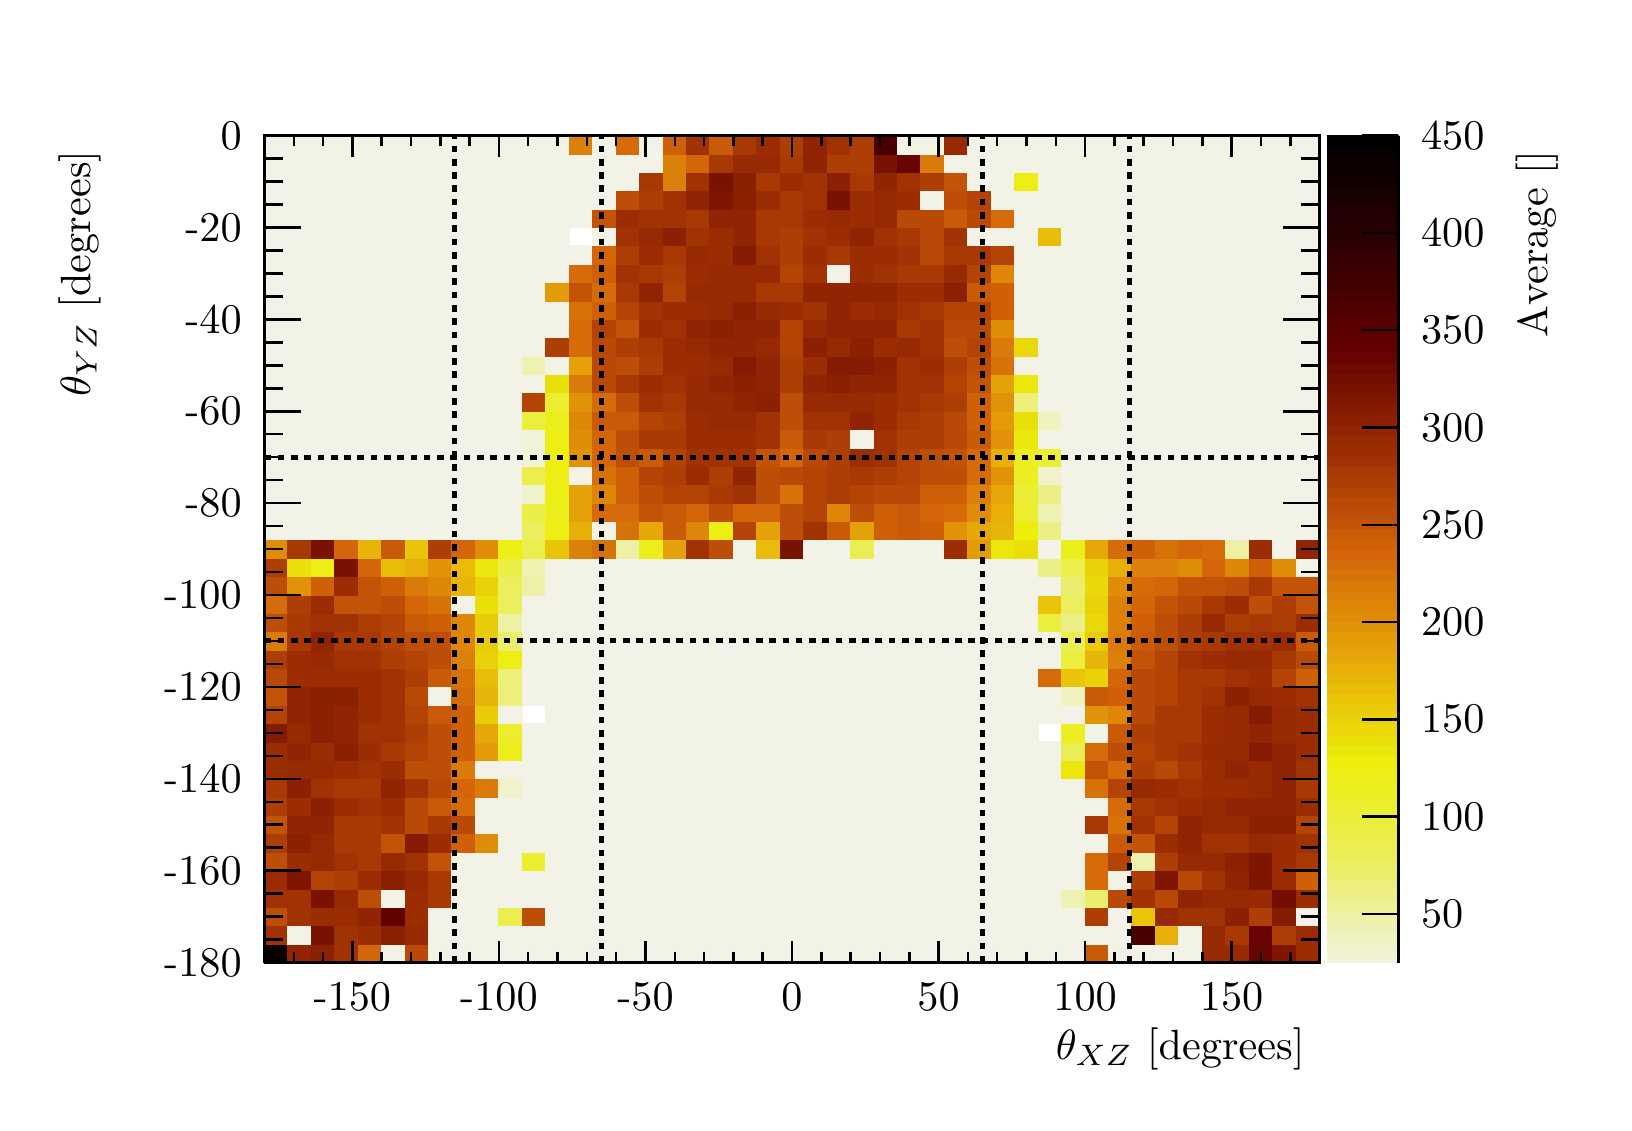
\begin{tikzpicture}
\pgfdeclareplotmark{cross} {
\pgfpathmoveto{\pgfpoint{-0.3\pgfplotmarksize}{\pgfplotmarksize}}
\pgfpathlineto{\pgfpoint{+0.3\pgfplotmarksize}{\pgfplotmarksize}}
\pgfpathlineto{\pgfpoint{+0.3\pgfplotmarksize}{0.3\pgfplotmarksize}}
\pgfpathlineto{\pgfpoint{+1\pgfplotmarksize}{0.3\pgfplotmarksize}}
\pgfpathlineto{\pgfpoint{+1\pgfplotmarksize}{-0.3\pgfplotmarksize}}
\pgfpathlineto{\pgfpoint{+0.3\pgfplotmarksize}{-0.3\pgfplotmarksize}}
\pgfpathlineto{\pgfpoint{+0.3\pgfplotmarksize}{-1.\pgfplotmarksize}}
\pgfpathlineto{\pgfpoint{-0.3\pgfplotmarksize}{-1.\pgfplotmarksize}}
\pgfpathlineto{\pgfpoint{-0.3\pgfplotmarksize}{-0.3\pgfplotmarksize}}
\pgfpathlineto{\pgfpoint{-1.\pgfplotmarksize}{-0.3\pgfplotmarksize}}
\pgfpathlineto{\pgfpoint{-1.\pgfplotmarksize}{0.3\pgfplotmarksize}}
\pgfpathlineto{\pgfpoint{-0.3\pgfplotmarksize}{0.3\pgfplotmarksize}}
\pgfpathclose
\pgfusepathqstroke
}
\pgfdeclareplotmark{cross*} {
\pgfpathmoveto{\pgfpoint{-0.3\pgfplotmarksize}{\pgfplotmarksize}}
\pgfpathlineto{\pgfpoint{+0.3\pgfplotmarksize}{\pgfplotmarksize}}
\pgfpathlineto{\pgfpoint{+0.3\pgfplotmarksize}{0.3\pgfplotmarksize}}
\pgfpathlineto{\pgfpoint{+1\pgfplotmarksize}{0.3\pgfplotmarksize}}
\pgfpathlineto{\pgfpoint{+1\pgfplotmarksize}{-0.3\pgfplotmarksize}}
\pgfpathlineto{\pgfpoint{+0.3\pgfplotmarksize}{-0.3\pgfplotmarksize}}
\pgfpathlineto{\pgfpoint{+0.3\pgfplotmarksize}{-1.\pgfplotmarksize}}
\pgfpathlineto{\pgfpoint{-0.3\pgfplotmarksize}{-1.\pgfplotmarksize}}
\pgfpathlineto{\pgfpoint{-0.3\pgfplotmarksize}{-0.3\pgfplotmarksize}}
\pgfpathlineto{\pgfpoint{-1.\pgfplotmarksize}{-0.3\pgfplotmarksize}}
\pgfpathlineto{\pgfpoint{-1.\pgfplotmarksize}{0.3\pgfplotmarksize}}
\pgfpathlineto{\pgfpoint{-0.3\pgfplotmarksize}{0.3\pgfplotmarksize}}
\pgfpathclose
\pgfusepathqfillstroke
}
\pgfdeclareplotmark{newstar} {
\pgfpathmoveto{\pgfqpoint{0pt}{\pgfplotmarksize}}
\pgfpathlineto{\pgfqpointpolar{44}{0.5\pgfplotmarksize}}
\pgfpathlineto{\pgfqpointpolar{18}{\pgfplotmarksize}}
\pgfpathlineto{\pgfqpointpolar{-20}{0.5\pgfplotmarksize}}
\pgfpathlineto{\pgfqpointpolar{-54}{\pgfplotmarksize}}
\pgfpathlineto{\pgfqpointpolar{-90}{0.5\pgfplotmarksize}}
\pgfpathlineto{\pgfqpointpolar{234}{\pgfplotmarksize}}
\pgfpathlineto{\pgfqpointpolar{198}{0.5\pgfplotmarksize}}
\pgfpathlineto{\pgfqpointpolar{162}{\pgfplotmarksize}}
\pgfpathlineto{\pgfqpointpolar{134}{0.5\pgfplotmarksize}}
\pgfpathclose
\pgfusepathqstroke
}
\pgfdeclareplotmark{newstar*} {
\pgfpathmoveto{\pgfqpoint{0pt}{\pgfplotmarksize}}
\pgfpathlineto{\pgfqpointpolar{44}{0.5\pgfplotmarksize}}
\pgfpathlineto{\pgfqpointpolar{18}{\pgfplotmarksize}}
\pgfpathlineto{\pgfqpointpolar{-20}{0.5\pgfplotmarksize}}
\pgfpathlineto{\pgfqpointpolar{-54}{\pgfplotmarksize}}
\pgfpathlineto{\pgfqpointpolar{-90}{0.5\pgfplotmarksize}}
\pgfpathlineto{\pgfqpointpolar{234}{\pgfplotmarksize}}
\pgfpathlineto{\pgfqpointpolar{198}{0.5\pgfplotmarksize}}
\pgfpathlineto{\pgfqpointpolar{162}{\pgfplotmarksize}}
\pgfpathlineto{\pgfqpointpolar{134}{0.5\pgfplotmarksize}}
\pgfpathclose
\pgfusepathqfillstroke
}
\definecolor{c}{rgb}{1,1,1};
\draw [color=c, fill=c] (0,0) rectangle (20,13.639);
\draw [color=c, fill=c] (3,1.77307) rectangle (16.4,12.2751);
\definecolor{c}{rgb}{0,0,0};
\draw [c,line width=0.9] (3,1.77307) -- (3,12.2751) -- (16.4,12.2751) -- (16.4,1.77307) -- (3,1.77307);
\definecolor{c}{rgb}{1,1,1};
\draw [color=c, fill=c] (3,1.77307) rectangle (16.4,12.2751);
\definecolor{c}{rgb}{0,0,0};
\draw [c,line width=0.9] (3,1.77307) -- (3,12.2751) -- (16.4,12.2751) -- (16.4,1.77307) -- (3,1.77307);
\definecolor{c}{rgb}{0.0386029,0,0.000857843};
\draw [color=c, fill=c] (3,1.77307) rectangle (3.29778,2.00644);
\definecolor{c}{rgb}{0.569853,0.143382,0.0102941};
\draw [color=c, fill=c] (3.29778,1.77307) rectangle (3.59556,2.00644);
\definecolor{c}{rgb}{0.548897,0.126838,0.00955882};
\draw [color=c, fill=c] (3.59556,1.77307) rectangle (3.89333,2.00644);
\definecolor{c}{rgb}{0.632353,0.197059,0.0139706};
\draw [color=c, fill=c] (3.89333,1.77307) rectangle (4.19111,2.00644);
\definecolor{c}{rgb}{0.831373,0.396078,0.0352941};
\draw [color=c, fill=c] (4.19111,1.77307) rectangle (4.48889,2.00644);
\definecolor{c}{rgb}{0.94902,0.952941,0.901961};
\draw [color=c, fill=c] (4.48889,1.77307) rectangle (4.78667,2.00644);
\definecolor{c}{rgb}{0.721569,0.286275,0.0235294};
\draw [color=c, fill=c] (4.78667,1.77307) rectangle (5.08444,2.00644);
\definecolor{c}{rgb}{0.94902,0.952941,0.901961};
\draw [color=c, fill=c] (5.08444,1.77307) rectangle (5.38222,2.00644);
\draw [color=c, fill=c] (5.38222,1.77307) rectangle (5.68,2.00644);
\draw [color=c, fill=c] (5.68,1.77307) rectangle (5.97778,2.00644);
\draw [color=c, fill=c] (5.97778,1.77307) rectangle (6.27556,2.00644);
\draw [color=c, fill=c] (6.27556,1.77307) rectangle (6.57333,2.00644);
\draw [color=c, fill=c] (6.57333,1.77307) rectangle (6.87111,2.00644);
\draw [color=c, fill=c] (6.87111,1.77307) rectangle (7.16889,2.00644);
\draw [color=c, fill=c] (7.16889,1.77307) rectangle (7.46667,2.00644);
\draw [color=c, fill=c] (7.46667,1.77307) rectangle (7.76444,2.00644);
\draw [color=c, fill=c] (7.76444,1.77307) rectangle (8.06222,2.00644);
\draw [color=c, fill=c] (8.06222,1.77307) rectangle (8.36,2.00644);
\draw [color=c, fill=c] (8.36,1.77307) rectangle (8.65778,2.00644);
\draw [color=c, fill=c] (8.65778,1.77307) rectangle (8.95556,2.00644);
\draw [color=c, fill=c] (8.95556,1.77307) rectangle (9.25333,2.00644);
\draw [color=c, fill=c] (9.25333,1.77307) rectangle (9.55111,2.00644);
\draw [color=c, fill=c] (9.55111,1.77307) rectangle (9.84889,2.00644);
\draw [color=c, fill=c] (9.84889,1.77307) rectangle (10.1467,2.00644);
\draw [color=c, fill=c] (10.1467,1.77307) rectangle (10.4444,2.00644);
\draw [color=c, fill=c] (10.4444,1.77307) rectangle (10.7422,2.00644);
\draw [color=c, fill=c] (10.7422,1.77307) rectangle (11.04,2.00644);
\draw [color=c, fill=c] (11.04,1.77307) rectangle (11.3378,2.00644);
\draw [color=c, fill=c] (11.3378,1.77307) rectangle (11.6356,2.00644);
\draw [color=c, fill=c] (11.6356,1.77307) rectangle (11.9333,2.00644);
\draw [color=c, fill=c] (11.9333,1.77307) rectangle (12.2311,2.00644);
\draw [color=c, fill=c] (12.2311,1.77307) rectangle (12.5289,2.00644);
\draw [color=c, fill=c] (12.5289,1.77307) rectangle (12.8267,2.00644);
\draw [color=c, fill=c] (12.8267,1.77307) rectangle (13.1244,2.00644);
\draw [color=c, fill=c] (13.1244,1.77307) rectangle (13.4222,2.00644);
\definecolor{c}{rgb}{0.790196,0.354902,0.0308824};
\draw [color=c, fill=c] (13.4222,1.77307) rectangle (13.72,2.00644);
\definecolor{c}{rgb}{0.94902,0.952941,0.901961};
\draw [color=c, fill=c] (13.72,1.77307) rectangle (14.0178,2.00644);
\draw [color=c, fill=c] (14.0178,1.77307) rectangle (14.3156,2.00644);
\draw [color=c, fill=c] (14.3156,1.77307) rectangle (14.6133,2.00644);
\draw [color=c, fill=c] (14.6133,1.77307) rectangle (14.9111,2.00644);
\definecolor{c}{rgb}{0.590809,0.159926,0.0110294};
\draw [color=c, fill=c] (14.9111,1.77307) rectangle (15.2089,2.00644);
\draw [color=c, fill=c] (15.2089,1.77307) rectangle (15.5067,2.00644);
\definecolor{c}{rgb}{0.409191,0.0165441,0.00465686};
\draw [color=c, fill=c] (15.5067,1.77307) rectangle (15.8044,2.00644);
\definecolor{c}{rgb}{0.5,0.0882353,0.00784314};
\draw [color=c, fill=c] (15.8044,1.77307) rectangle (16.1022,2.00644);
\definecolor{c}{rgb}{0.611765,0.176471,0.0117647};
\draw [color=c, fill=c] (16.1022,1.77307) rectangle (16.4,2.00644);
\definecolor{c}{rgb}{0.632353,0.197059,0.0139706};
\draw [color=c, fill=c] (3,2.00644) rectangle (3.29778,2.23982);
\definecolor{c}{rgb}{0.94902,0.952941,0.901961};
\draw [color=c, fill=c] (3.29778,2.00644) rectangle (3.59556,2.23982);
\definecolor{c}{rgb}{0.479044,0.0716912,0.00710784};
\draw [color=c, fill=c] (3.59556,2.00644) rectangle (3.89333,2.23982);
\definecolor{c}{rgb}{0.632353,0.197059,0.0139706};
\draw [color=c, fill=c] (3.89333,2.00644) rectangle (4.19111,2.23982);
\definecolor{c}{rgb}{0.611765,0.176471,0.0117647};
\draw [color=c, fill=c] (4.19111,2.00644) rectangle (4.48889,2.23982);
\definecolor{c}{rgb}{0.548897,0.126838,0.00955882};
\draw [color=c, fill=c] (4.48889,2.00644) rectangle (4.78667,2.23982);
\definecolor{c}{rgb}{0.590809,0.159926,0.0110294};
\draw [color=c, fill=c] (4.78667,2.00644) rectangle (5.08444,2.23982);
\definecolor{c}{rgb}{0.94902,0.952941,0.901961};
\draw [color=c, fill=c] (5.08444,2.00644) rectangle (5.38222,2.23982);
\draw [color=c, fill=c] (5.38222,2.00644) rectangle (5.68,2.23982);
\draw [color=c, fill=c] (5.68,2.00644) rectangle (5.97778,2.23982);
\draw [color=c, fill=c] (5.97778,2.00644) rectangle (6.27556,2.23982);
\draw [color=c, fill=c] (6.27556,2.00644) rectangle (6.57333,2.23982);
\draw [color=c, fill=c] (6.57333,2.00644) rectangle (6.87111,2.23982);
\draw [color=c, fill=c] (6.87111,2.00644) rectangle (7.16889,2.23982);
\draw [color=c, fill=c] (7.16889,2.00644) rectangle (7.46667,2.23982);
\draw [color=c, fill=c] (7.46667,2.00644) rectangle (7.76444,2.23982);
\draw [color=c, fill=c] (7.76444,2.00644) rectangle (8.06222,2.23982);
\draw [color=c, fill=c] (8.06222,2.00644) rectangle (8.36,2.23982);
\draw [color=c, fill=c] (8.36,2.00644) rectangle (8.65778,2.23982);
\draw [color=c, fill=c] (8.65778,2.00644) rectangle (8.95556,2.23982);
\draw [color=c, fill=c] (8.95556,2.00644) rectangle (9.25333,2.23982);
\draw [color=c, fill=c] (9.25333,2.00644) rectangle (9.55111,2.23982);
\draw [color=c, fill=c] (9.55111,2.00644) rectangle (9.84889,2.23982);
\draw [color=c, fill=c] (9.84889,2.00644) rectangle (10.1467,2.23982);
\draw [color=c, fill=c] (10.1467,2.00644) rectangle (10.4444,2.23982);
\draw [color=c, fill=c] (10.4444,2.00644) rectangle (10.7422,2.23982);
\draw [color=c, fill=c] (10.7422,2.00644) rectangle (11.04,2.23982);
\draw [color=c, fill=c] (11.04,2.00644) rectangle (11.3378,2.23982);
\draw [color=c, fill=c] (11.3378,2.00644) rectangle (11.6356,2.23982);
\draw [color=c, fill=c] (11.6356,2.00644) rectangle (11.9333,2.23982);
\draw [color=c, fill=c] (11.9333,2.00644) rectangle (12.2311,2.23982);
\draw [color=c, fill=c] (12.2311,2.00644) rectangle (12.5289,2.23982);
\draw [color=c, fill=c] (12.5289,2.00644) rectangle (12.8267,2.23982);
\draw [color=c, fill=c] (12.8267,2.00644) rectangle (13.1244,2.23982);
\draw [color=c, fill=c] (13.1244,2.00644) rectangle (13.4222,2.23982);
\draw [color=c, fill=c] (13.4222,2.00644) rectangle (13.72,2.23982);
\draw [color=c, fill=c] (13.72,2.00644) rectangle (14.0178,2.23982);
\definecolor{c}{rgb}{0.282353,0,0.00392157};
\draw [color=c, fill=c] (14.0178,2.00644) rectangle (14.3156,2.23982);
\definecolor{c}{rgb}{0.904534,0.684559,0.0324755};
\draw [color=c, fill=c] (14.3156,2.00644) rectangle (14.6133,2.23982);
\definecolor{c}{rgb}{0.94902,0.952941,0.901961};
\draw [color=c, fill=c] (14.6133,2.00644) rectangle (14.9111,2.23982);
\definecolor{c}{rgb}{0.590809,0.159926,0.0110294};
\draw [color=c, fill=c] (14.9111,2.00644) rectangle (15.2089,2.23982);
\definecolor{c}{rgb}{0.659804,0.22451,0.0169118};
\draw [color=c, fill=c] (15.2089,2.00644) rectangle (15.5067,2.23982);
\definecolor{c}{rgb}{0.409191,0.0165441,0.00465686};
\draw [color=c, fill=c] (15.5067,2.00644) rectangle (15.8044,2.23982);
\definecolor{c}{rgb}{0.680392,0.245098,0.0191176};
\draw [color=c, fill=c] (15.8044,2.00644) rectangle (16.1022,2.23982);
\definecolor{c}{rgb}{0.611765,0.176471,0.0117647};
\draw [color=c, fill=c] (16.1022,2.00644) rectangle (16.4,2.23982);
\definecolor{c}{rgb}{0.742157,0.306863,0.0257353};
\draw [color=c, fill=c] (3,2.23982) rectangle (3.29778,2.4732);
\definecolor{c}{rgb}{0.632353,0.197059,0.0139706};
\draw [color=c, fill=c] (3.29778,2.23982) rectangle (3.59556,2.4732);
\definecolor{c}{rgb}{0.611765,0.176471,0.0117647};
\draw [color=c, fill=c] (3.59556,2.23982) rectangle (3.89333,2.4732);
\draw [color=c, fill=c] (3.89333,2.23982) rectangle (4.19111,2.4732);
\definecolor{c}{rgb}{0.569853,0.143382,0.0102941};
\draw [color=c, fill=c] (4.19111,2.23982) rectangle (4.48889,2.4732);
\definecolor{c}{rgb}{0.388235,0,0.00392157};
\draw [color=c, fill=c] (4.48889,2.23982) rectangle (4.78667,2.4732);
\definecolor{c}{rgb}{0.611765,0.176471,0.0117647};
\draw [color=c, fill=c] (4.78667,2.23982) rectangle (5.08444,2.4732);
\definecolor{c}{rgb}{0.94902,0.952941,0.901961};
\draw [color=c, fill=c] (5.08444,2.23982) rectangle (5.38222,2.4732);
\draw [color=c, fill=c] (5.38222,2.23982) rectangle (5.68,2.4732);
\draw [color=c, fill=c] (5.68,2.23982) rectangle (5.97778,2.4732);
\definecolor{c}{rgb}{0.920221,0.933333,0.30049};
\draw [color=c, fill=c] (5.97778,2.23982) rectangle (6.27556,2.4732);
\definecolor{c}{rgb}{0.742157,0.306863,0.0257353};
\draw [color=c, fill=c] (6.27556,2.23982) rectangle (6.57333,2.4732);
\definecolor{c}{rgb}{0.94902,0.952941,0.901961};
\draw [color=c, fill=c] (6.57333,2.23982) rectangle (6.87111,2.4732);
\draw [color=c, fill=c] (6.87111,2.23982) rectangle (7.16889,2.4732);
\draw [color=c, fill=c] (7.16889,2.23982) rectangle (7.46667,2.4732);
\draw [color=c, fill=c] (7.46667,2.23982) rectangle (7.76444,2.4732);
\draw [color=c, fill=c] (7.76444,2.23982) rectangle (8.06222,2.4732);
\draw [color=c, fill=c] (8.06222,2.23982) rectangle (8.36,2.4732);
\draw [color=c, fill=c] (8.36,2.23982) rectangle (8.65778,2.4732);
\draw [color=c, fill=c] (8.65778,2.23982) rectangle (8.95556,2.4732);
\draw [color=c, fill=c] (8.95556,2.23982) rectangle (9.25333,2.4732);
\draw [color=c, fill=c] (9.25333,2.23982) rectangle (9.55111,2.4732);
\draw [color=c, fill=c] (9.55111,2.23982) rectangle (9.84889,2.4732);
\draw [color=c, fill=c] (9.84889,2.23982) rectangle (10.1467,2.4732);
\draw [color=c, fill=c] (10.1467,2.23982) rectangle (10.4444,2.4732);
\draw [color=c, fill=c] (10.4444,2.23982) rectangle (10.7422,2.4732);
\draw [color=c, fill=c] (10.7422,2.23982) rectangle (11.04,2.4732);
\draw [color=c, fill=c] (11.04,2.23982) rectangle (11.3378,2.4732);
\draw [color=c, fill=c] (11.3378,2.23982) rectangle (11.6356,2.4732);
\draw [color=c, fill=c] (11.6356,2.23982) rectangle (11.9333,2.4732);
\draw [color=c, fill=c] (11.9333,2.23982) rectangle (12.2311,2.4732);
\draw [color=c, fill=c] (12.2311,2.23982) rectangle (12.5289,2.4732);
\draw [color=c, fill=c] (12.5289,2.23982) rectangle (12.8267,2.4732);
\draw [color=c, fill=c] (12.8267,2.23982) rectangle (13.1244,2.4732);
\draw [color=c, fill=c] (13.1244,2.23982) rectangle (13.4222,2.4732);
\definecolor{c}{rgb}{0.680392,0.245098,0.0191176};
\draw [color=c, fill=c] (13.4222,2.23982) rectangle (13.72,2.4732);
\definecolor{c}{rgb}{0.94902,0.952941,0.901961};
\draw [color=c, fill=c] (13.72,2.23982) rectangle (14.0178,2.4732);
\definecolor{c}{rgb}{0.913113,0.770343,0.036152};
\draw [color=c, fill=c] (14.0178,2.23982) rectangle (14.3156,2.4732);
\definecolor{c}{rgb}{0.590809,0.159926,0.0110294};
\draw [color=c, fill=c] (14.3156,2.23982) rectangle (14.6133,2.4732);
\definecolor{c}{rgb}{0.632353,0.197059,0.0139706};
\draw [color=c, fill=c] (14.6133,2.23982) rectangle (14.9111,2.4732);
\draw [color=c, fill=c] (14.9111,2.23982) rectangle (15.2089,2.4732);
\definecolor{c}{rgb}{0.548897,0.126838,0.00955882};
\draw [color=c, fill=c] (15.2089,2.23982) rectangle (15.5067,2.4732);
\definecolor{c}{rgb}{0.680392,0.245098,0.0191176};
\draw [color=c, fill=c] (15.5067,2.23982) rectangle (15.8044,2.4732);
\definecolor{c}{rgb}{0.520956,0.104779,0.00857843};
\draw [color=c, fill=c] (15.8044,2.23982) rectangle (16.1022,2.4732);
\definecolor{c}{rgb}{0.94902,0.952941,0.901961};
\draw [color=c, fill=c] (16.1022,2.23982) rectangle (16.4,2.4732);
\definecolor{c}{rgb}{0.632353,0.197059,0.0139706};
\draw [color=c, fill=c] (3,2.4732) rectangle (3.29778,2.70658);
\draw [color=c, fill=c] (3.29778,2.4732) rectangle (3.59556,2.70658);
\definecolor{c}{rgb}{0.479044,0.0716912,0.00710784};
\draw [color=c, fill=c] (3.59556,2.4732) rectangle (3.89333,2.70658);
\definecolor{c}{rgb}{0.590809,0.159926,0.0110294};
\draw [color=c, fill=c] (3.89333,2.4732) rectangle (4.19111,2.70658);
\definecolor{c}{rgb}{0.742157,0.306863,0.0257353};
\draw [color=c, fill=c] (4.19111,2.4732) rectangle (4.48889,2.70658);
\definecolor{c}{rgb}{0.94902,0.952941,0.901961};
\draw [color=c, fill=c] (4.48889,2.4732) rectangle (4.78667,2.70658);
\definecolor{c}{rgb}{0.611765,0.176471,0.0117647};
\draw [color=c, fill=c] (4.78667,2.4732) rectangle (5.08444,2.70658);
\definecolor{c}{rgb}{0.659804,0.22451,0.0169118};
\draw [color=c, fill=c] (5.08444,2.4732) rectangle (5.38222,2.70658);
\definecolor{c}{rgb}{0.94902,0.952941,0.901961};
\draw [color=c, fill=c] (5.38222,2.4732) rectangle (5.68,2.70658);
\draw [color=c, fill=c] (5.68,2.4732) rectangle (5.97778,2.70658);
\draw [color=c, fill=c] (5.97778,2.4732) rectangle (6.27556,2.70658);
\draw [color=c, fill=c] (6.27556,2.4732) rectangle (6.57333,2.70658);
\draw [color=c, fill=c] (6.57333,2.4732) rectangle (6.87111,2.70658);
\draw [color=c, fill=c] (6.87111,2.4732) rectangle (7.16889,2.70658);
\draw [color=c, fill=c] (7.16889,2.4732) rectangle (7.46667,2.70658);
\draw [color=c, fill=c] (7.46667,2.4732) rectangle (7.76444,2.70658);
\draw [color=c, fill=c] (7.76444,2.4732) rectangle (8.06222,2.70658);
\draw [color=c, fill=c] (8.06222,2.4732) rectangle (8.36,2.70658);
\draw [color=c, fill=c] (8.36,2.4732) rectangle (8.65778,2.70658);
\draw [color=c, fill=c] (8.65778,2.4732) rectangle (8.95556,2.70658);
\draw [color=c, fill=c] (8.95556,2.4732) rectangle (9.25333,2.70658);
\draw [color=c, fill=c] (9.25333,2.4732) rectangle (9.55111,2.70658);
\draw [color=c, fill=c] (9.55111,2.4732) rectangle (9.84889,2.70658);
\draw [color=c, fill=c] (9.84889,2.4732) rectangle (10.1467,2.70658);
\draw [color=c, fill=c] (10.1467,2.4732) rectangle (10.4444,2.70658);
\draw [color=c, fill=c] (10.4444,2.4732) rectangle (10.7422,2.70658);
\draw [color=c, fill=c] (10.7422,2.4732) rectangle (11.04,2.70658);
\draw [color=c, fill=c] (11.04,2.4732) rectangle (11.3378,2.70658);
\draw [color=c, fill=c] (11.3378,2.4732) rectangle (11.6356,2.70658);
\draw [color=c, fill=c] (11.6356,2.4732) rectangle (11.9333,2.70658);
\draw [color=c, fill=c] (11.9333,2.4732) rectangle (12.2311,2.70658);
\draw [color=c, fill=c] (12.2311,2.4732) rectangle (12.5289,2.70658);
\draw [color=c, fill=c] (12.5289,2.4732) rectangle (12.8267,2.70658);
\draw [color=c, fill=c] (12.8267,2.4732) rectangle (13.1244,2.70658);
\definecolor{c}{rgb}{0.936875,0.945351,0.697027};
\draw [color=c, fill=c] (13.1244,2.4732) rectangle (13.4222,2.70658);
\definecolor{c}{rgb}{0.920683,0.935231,0.423782};
\draw [color=c, fill=c] (13.4222,2.4732) rectangle (13.72,2.70658);
\definecolor{c}{rgb}{0.721569,0.286275,0.0235294};
\draw [color=c, fill=c] (13.72,2.4732) rectangle (14.0178,2.70658);
\definecolor{c}{rgb}{0.632353,0.197059,0.0139706};
\draw [color=c, fill=c] (14.0178,2.4732) rectangle (14.3156,2.70658);
\definecolor{c}{rgb}{0.721569,0.286275,0.0235294};
\draw [color=c, fill=c] (14.3156,2.4732) rectangle (14.6133,2.70658);
\definecolor{c}{rgb}{0.569853,0.143382,0.0102941};
\draw [color=c, fill=c] (14.6133,2.4732) rectangle (14.9111,2.70658);
\definecolor{c}{rgb}{0.590809,0.159926,0.0110294};
\draw [color=c, fill=c] (14.9111,2.4732) rectangle (15.2089,2.70658);
\draw [color=c, fill=c] (15.2089,2.4732) rectangle (15.5067,2.70658);
\draw [color=c, fill=c] (15.5067,2.4732) rectangle (15.8044,2.70658);
\definecolor{c}{rgb}{0.458088,0.0551471,0.00637255};
\draw [color=c, fill=c] (15.8044,2.4732) rectangle (16.1022,2.70658);
\definecolor{c}{rgb}{0.611765,0.176471,0.0117647};
\draw [color=c, fill=c] (16.1022,2.4732) rectangle (16.4,2.70658);
\draw [color=c, fill=c] (3,2.70658) rectangle (3.29778,2.93996);
\definecolor{c}{rgb}{0.5,0.0882353,0.00784314};
\draw [color=c, fill=c] (3.29778,2.70658) rectangle (3.59556,2.93996);
\definecolor{c}{rgb}{0.70098,0.265686,0.0213235};
\draw [color=c, fill=c] (3.59556,2.70658) rectangle (3.89333,2.93996);
\definecolor{c}{rgb}{0.680392,0.245098,0.0191176};
\draw [color=c, fill=c] (3.89333,2.70658) rectangle (4.19111,2.93996);
\definecolor{c}{rgb}{0.611765,0.176471,0.0117647};
\draw [color=c, fill=c] (4.19111,2.70658) rectangle (4.48889,2.93996);
\definecolor{c}{rgb}{0.548897,0.126838,0.00955882};
\draw [color=c, fill=c] (4.48889,2.70658) rectangle (4.78667,2.93996);
\definecolor{c}{rgb}{0.590809,0.159926,0.0110294};
\draw [color=c, fill=c] (4.78667,2.70658) rectangle (5.08444,2.93996);
\definecolor{c}{rgb}{0.659804,0.22451,0.0169118};
\draw [color=c, fill=c] (5.08444,2.70658) rectangle (5.38222,2.93996);
\definecolor{c}{rgb}{0.94902,0.952941,0.901961};
\draw [color=c, fill=c] (5.38222,2.70658) rectangle (5.68,2.93996);
\draw [color=c, fill=c] (5.68,2.70658) rectangle (5.97778,2.93996);
\draw [color=c, fill=c] (5.97778,2.70658) rectangle (6.27556,2.93996);
\draw [color=c, fill=c] (6.27556,2.70658) rectangle (6.57333,2.93996);
\draw [color=c, fill=c] (6.57333,2.70658) rectangle (6.87111,2.93996);
\draw [color=c, fill=c] (6.87111,2.70658) rectangle (7.16889,2.93996);
\draw [color=c, fill=c] (7.16889,2.70658) rectangle (7.46667,2.93996);
\draw [color=c, fill=c] (7.46667,2.70658) rectangle (7.76444,2.93996);
\draw [color=c, fill=c] (7.76444,2.70658) rectangle (8.06222,2.93996);
\draw [color=c, fill=c] (8.06222,2.70658) rectangle (8.36,2.93996);
\draw [color=c, fill=c] (8.36,2.70658) rectangle (8.65778,2.93996);
\draw [color=c, fill=c] (8.65778,2.70658) rectangle (8.95556,2.93996);
\draw [color=c, fill=c] (8.95556,2.70658) rectangle (9.25333,2.93996);
\draw [color=c, fill=c] (9.25333,2.70658) rectangle (9.55111,2.93996);
\draw [color=c, fill=c] (9.55111,2.70658) rectangle (9.84889,2.93996);
\draw [color=c, fill=c] (9.84889,2.70658) rectangle (10.1467,2.93996);
\draw [color=c, fill=c] (10.1467,2.70658) rectangle (10.4444,2.93996);
\draw [color=c, fill=c] (10.4444,2.70658) rectangle (10.7422,2.93996);
\draw [color=c, fill=c] (10.7422,2.70658) rectangle (11.04,2.93996);
\draw [color=c, fill=c] (11.04,2.70658) rectangle (11.3378,2.93996);
\draw [color=c, fill=c] (11.3378,2.70658) rectangle (11.6356,2.93996);
\draw [color=c, fill=c] (11.6356,2.70658) rectangle (11.9333,2.93996);
\draw [color=c, fill=c] (11.9333,2.70658) rectangle (12.2311,2.93996);
\draw [color=c, fill=c] (12.2311,2.70658) rectangle (12.5289,2.93996);
\draw [color=c, fill=c] (12.5289,2.70658) rectangle (12.8267,2.93996);
\draw [color=c, fill=c] (12.8267,2.70658) rectangle (13.1244,2.93996);
\draw [color=c, fill=c] (13.1244,2.70658) rectangle (13.4222,2.93996);
\definecolor{c}{rgb}{0.83799,0.420711,0.0349265};
\draw [color=c, fill=c] (13.4222,2.70658) rectangle (13.72,2.93996);
\definecolor{c}{rgb}{0.94902,0.952941,0.901961};
\draw [color=c, fill=c] (13.72,2.70658) rectangle (14.0178,2.93996);
\definecolor{c}{rgb}{0.680392,0.245098,0.0191176};
\draw [color=c, fill=c] (14.0178,2.70658) rectangle (14.3156,2.93996);
\definecolor{c}{rgb}{0.5,0.0882353,0.00784314};
\draw [color=c, fill=c] (14.3156,2.70658) rectangle (14.6133,2.93996);
\definecolor{c}{rgb}{0.721569,0.286275,0.0235294};
\draw [color=c, fill=c] (14.6133,2.70658) rectangle (14.9111,2.93996);
\definecolor{c}{rgb}{0.632353,0.197059,0.0139706};
\draw [color=c, fill=c] (14.9111,2.70658) rectangle (15.2089,2.93996);
\definecolor{c}{rgb}{0.569853,0.143382,0.0102941};
\draw [color=c, fill=c] (15.2089,2.70658) rectangle (15.5067,2.93996);
\definecolor{c}{rgb}{0.5,0.0882353,0.00784314};
\draw [color=c, fill=c] (15.5067,2.70658) rectangle (15.8044,2.93996);
\definecolor{c}{rgb}{0.611765,0.176471,0.0117647};
\draw [color=c, fill=c] (15.8044,2.70658) rectangle (16.1022,2.93996);
\definecolor{c}{rgb}{0.810784,0.37549,0.0330882};
\draw [color=c, fill=c] (16.1022,2.70658) rectangle (16.4,2.93996);
\definecolor{c}{rgb}{0.742157,0.306863,0.0257353};
\draw [color=c, fill=c] (3,2.93996) rectangle (3.29778,3.17333);
\definecolor{c}{rgb}{0.611765,0.176471,0.0117647};
\draw [color=c, fill=c] (3.29778,2.93996) rectangle (3.59556,3.17333);
\definecolor{c}{rgb}{0.590809,0.159926,0.0110294};
\draw [color=c, fill=c] (3.59556,2.93996) rectangle (3.89333,3.17333);
\definecolor{c}{rgb}{0.632353,0.197059,0.0139706};
\draw [color=c, fill=c] (3.89333,2.93996) rectangle (4.19111,3.17333);
\definecolor{c}{rgb}{0.659804,0.22451,0.0169118};
\draw [color=c, fill=c] (4.19111,2.93996) rectangle (4.48889,3.17333);
\definecolor{c}{rgb}{0.590809,0.159926,0.0110294};
\draw [color=c, fill=c] (4.48889,2.93996) rectangle (4.78667,3.17333);
\definecolor{c}{rgb}{0.632353,0.197059,0.0139706};
\draw [color=c, fill=c] (4.78667,2.93996) rectangle (5.08444,3.17333);
\definecolor{c}{rgb}{0.762745,0.327451,0.0279412};
\draw [color=c, fill=c] (5.08444,2.93996) rectangle (5.38222,3.17333);
\definecolor{c}{rgb}{0.94902,0.952941,0.901961};
\draw [color=c, fill=c] (5.38222,2.93996) rectangle (5.68,3.17333);
\draw [color=c, fill=c] (5.68,2.93996) rectangle (5.97778,3.17333);
\draw [color=c, fill=c] (5.97778,2.93996) rectangle (6.27556,3.17333);
\definecolor{c}{rgb}{0.924632,0.933333,0.176961};
\draw [color=c, fill=c] (6.27556,2.93996) rectangle (6.57333,3.17333);
\definecolor{c}{rgb}{0.94902,0.952941,0.901961};
\draw [color=c, fill=c] (6.57333,2.93996) rectangle (6.87111,3.17333);
\draw [color=c, fill=c] (6.87111,2.93996) rectangle (7.16889,3.17333);
\draw [color=c, fill=c] (7.16889,2.93996) rectangle (7.46667,3.17333);
\draw [color=c, fill=c] (7.46667,2.93996) rectangle (7.76444,3.17333);
\draw [color=c, fill=c] (7.76444,2.93996) rectangle (8.06222,3.17333);
\draw [color=c, fill=c] (8.06222,2.93996) rectangle (8.36,3.17333);
\draw [color=c, fill=c] (8.36,2.93996) rectangle (8.65778,3.17333);
\draw [color=c, fill=c] (8.65778,2.93996) rectangle (8.95556,3.17333);
\draw [color=c, fill=c] (8.95556,2.93996) rectangle (9.25333,3.17333);
\draw [color=c, fill=c] (9.25333,2.93996) rectangle (9.55111,3.17333);
\draw [color=c, fill=c] (9.55111,2.93996) rectangle (9.84889,3.17333);
\draw [color=c, fill=c] (9.84889,2.93996) rectangle (10.1467,3.17333);
\draw [color=c, fill=c] (10.1467,2.93996) rectangle (10.4444,3.17333);
\draw [color=c, fill=c] (10.4444,2.93996) rectangle (10.7422,3.17333);
\draw [color=c, fill=c] (10.7422,2.93996) rectangle (11.04,3.17333);
\draw [color=c, fill=c] (11.04,2.93996) rectangle (11.3378,3.17333);
\draw [color=c, fill=c] (11.3378,2.93996) rectangle (11.6356,3.17333);
\draw [color=c, fill=c] (11.6356,2.93996) rectangle (11.9333,3.17333);
\draw [color=c, fill=c] (11.9333,2.93996) rectangle (12.2311,3.17333);
\draw [color=c, fill=c] (12.2311,2.93996) rectangle (12.5289,3.17333);
\draw [color=c, fill=c] (12.5289,2.93996) rectangle (12.8267,3.17333);
\draw [color=c, fill=c] (12.8267,2.93996) rectangle (13.1244,3.17333);
\draw [color=c, fill=c] (13.1244,2.93996) rectangle (13.4222,3.17333);
\definecolor{c}{rgb}{0.83799,0.420711,0.0349265};
\draw [color=c, fill=c] (13.4222,2.93996) rectangle (13.72,3.17333);
\definecolor{c}{rgb}{0.70098,0.265686,0.0213235};
\draw [color=c, fill=c] (13.72,2.93996) rectangle (14.0178,3.17333);
\definecolor{c}{rgb}{0.936875,0.945351,0.697027};
\draw [color=c, fill=c] (14.0178,2.93996) rectangle (14.3156,3.17333);
\definecolor{c}{rgb}{0.680392,0.245098,0.0191176};
\draw [color=c, fill=c] (14.3156,2.93996) rectangle (14.6133,3.17333);
\definecolor{c}{rgb}{0.590809,0.159926,0.0110294};
\draw [color=c, fill=c] (14.6133,2.93996) rectangle (14.9111,3.17333);
\draw [color=c, fill=c] (14.9111,2.93996) rectangle (15.2089,3.17333);
\definecolor{c}{rgb}{0.548897,0.126838,0.00955882};
\draw [color=c, fill=c] (15.2089,2.93996) rectangle (15.5067,3.17333);
\definecolor{c}{rgb}{0.5,0.0882353,0.00784314};
\draw [color=c, fill=c] (15.5067,2.93996) rectangle (15.8044,3.17333);
\definecolor{c}{rgb}{0.611765,0.176471,0.0117647};
\draw [color=c, fill=c] (15.8044,2.93996) rectangle (16.1022,3.17333);
\definecolor{c}{rgb}{0.659804,0.22451,0.0169118};
\draw [color=c, fill=c] (16.1022,2.93996) rectangle (16.4,3.17333);
\definecolor{c}{rgb}{0.680392,0.245098,0.0191176};
\draw [color=c, fill=c] (3,3.17333) rectangle (3.29778,3.40671);
\definecolor{c}{rgb}{0.548897,0.126838,0.00955882};
\draw [color=c, fill=c] (3.29778,3.17333) rectangle (3.59556,3.40671);
\definecolor{c}{rgb}{0.590809,0.159926,0.0110294};
\draw [color=c, fill=c] (3.59556,3.17333) rectangle (3.89333,3.40671);
\definecolor{c}{rgb}{0.659804,0.22451,0.0169118};
\draw [color=c, fill=c] (3.89333,3.17333) rectangle (4.19111,3.40671);
\draw [color=c, fill=c] (4.19111,3.17333) rectangle (4.48889,3.40671);
\definecolor{c}{rgb}{0.762745,0.327451,0.0279412};
\draw [color=c, fill=c] (4.48889,3.17333) rectangle (4.78667,3.40671);
\definecolor{c}{rgb}{0.520956,0.104779,0.00857843};
\draw [color=c, fill=c] (4.78667,3.17333) rectangle (5.08444,3.40671);
\definecolor{c}{rgb}{0.611765,0.176471,0.0117647};
\draw [color=c, fill=c] (5.08444,3.17333) rectangle (5.38222,3.40671);
\definecolor{c}{rgb}{0.810784,0.37549,0.0330882};
\draw [color=c, fill=c] (5.38222,3.17333) rectangle (5.68,3.40671);
\definecolor{c}{rgb}{0.873284,0.552083,0.0329657};
\draw [color=c, fill=c] (5.68,3.17333) rectangle (5.97778,3.40671);
\definecolor{c}{rgb}{0.94902,0.952941,0.901961};
\draw [color=c, fill=c] (5.97778,3.17333) rectangle (6.27556,3.40671);
\draw [color=c, fill=c] (6.27556,3.17333) rectangle (6.57333,3.40671);
\draw [color=c, fill=c] (6.57333,3.17333) rectangle (6.87111,3.40671);
\draw [color=c, fill=c] (6.87111,3.17333) rectangle (7.16889,3.40671);
\draw [color=c, fill=c] (7.16889,3.17333) rectangle (7.46667,3.40671);
\draw [color=c, fill=c] (7.46667,3.17333) rectangle (7.76444,3.40671);
\draw [color=c, fill=c] (7.76444,3.17333) rectangle (8.06222,3.40671);
\draw [color=c, fill=c] (8.06222,3.17333) rectangle (8.36,3.40671);
\draw [color=c, fill=c] (8.36,3.17333) rectangle (8.65778,3.40671);
\draw [color=c, fill=c] (8.65778,3.17333) rectangle (8.95556,3.40671);
\draw [color=c, fill=c] (8.95556,3.17333) rectangle (9.25333,3.40671);
\draw [color=c, fill=c] (9.25333,3.17333) rectangle (9.55111,3.40671);
\draw [color=c, fill=c] (9.55111,3.17333) rectangle (9.84889,3.40671);
\draw [color=c, fill=c] (9.84889,3.17333) rectangle (10.1467,3.40671);
\draw [color=c, fill=c] (10.1467,3.17333) rectangle (10.4444,3.40671);
\draw [color=c, fill=c] (10.4444,3.17333) rectangle (10.7422,3.40671);
\draw [color=c, fill=c] (10.7422,3.17333) rectangle (11.04,3.40671);
\draw [color=c, fill=c] (11.04,3.17333) rectangle (11.3378,3.40671);
\draw [color=c, fill=c] (11.3378,3.17333) rectangle (11.6356,3.40671);
\draw [color=c, fill=c] (11.6356,3.17333) rectangle (11.9333,3.40671);
\draw [color=c, fill=c] (11.9333,3.17333) rectangle (12.2311,3.40671);
\draw [color=c, fill=c] (12.2311,3.17333) rectangle (12.5289,3.40671);
\draw [color=c, fill=c] (12.5289,3.17333) rectangle (12.8267,3.40671);
\draw [color=c, fill=c] (12.8267,3.17333) rectangle (13.1244,3.40671);
\draw [color=c, fill=c] (13.1244,3.17333) rectangle (13.4222,3.40671);
\draw [color=c, fill=c] (13.4222,3.17333) rectangle (13.72,3.40671);
\definecolor{c}{rgb}{0.790196,0.354902,0.0308824};
\draw [color=c, fill=c] (13.72,3.17333) rectangle (14.0178,3.40671);
\definecolor{c}{rgb}{0.762745,0.327451,0.0279412};
\draw [color=c, fill=c] (14.0178,3.17333) rectangle (14.3156,3.40671);
\definecolor{c}{rgb}{0.611765,0.176471,0.0117647};
\draw [color=c, fill=c] (14.3156,3.17333) rectangle (14.6133,3.40671);
\definecolor{c}{rgb}{0.569853,0.143382,0.0102941};
\draw [color=c, fill=c] (14.6133,3.17333) rectangle (14.9111,3.40671);
\definecolor{c}{rgb}{0.632353,0.197059,0.0139706};
\draw [color=c, fill=c] (14.9111,3.17333) rectangle (15.2089,3.40671);
\draw [color=c, fill=c] (15.2089,3.17333) rectangle (15.5067,3.40671);
\definecolor{c}{rgb}{0.590809,0.159926,0.0110294};
\draw [color=c, fill=c] (15.5067,3.17333) rectangle (15.8044,3.40671);
\definecolor{c}{rgb}{0.611765,0.176471,0.0117647};
\draw [color=c, fill=c] (15.8044,3.17333) rectangle (16.1022,3.40671);
\definecolor{c}{rgb}{0.632353,0.197059,0.0139706};
\draw [color=c, fill=c] (16.1022,3.17333) rectangle (16.4,3.40671);
\definecolor{c}{rgb}{0.762745,0.327451,0.0279412};
\draw [color=c, fill=c] (3,3.40671) rectangle (3.29778,3.64009);
\definecolor{c}{rgb}{0.569853,0.143382,0.0102941};
\draw [color=c, fill=c] (3.29778,3.40671) rectangle (3.59556,3.64009);
\draw [color=c, fill=c] (3.59556,3.40671) rectangle (3.89333,3.64009);
\definecolor{c}{rgb}{0.659804,0.22451,0.0169118};
\draw [color=c, fill=c] (3.89333,3.40671) rectangle (4.19111,3.64009);
\draw [color=c, fill=c] (4.19111,3.40671) rectangle (4.48889,3.64009);
\definecolor{c}{rgb}{0.632353,0.197059,0.0139706};
\draw [color=c, fill=c] (4.48889,3.40671) rectangle (4.78667,3.64009);
\definecolor{c}{rgb}{0.721569,0.286275,0.0235294};
\draw [color=c, fill=c] (4.78667,3.40671) rectangle (5.08444,3.64009);
\definecolor{c}{rgb}{0.659804,0.22451,0.0169118};
\draw [color=c, fill=c] (5.08444,3.40671) rectangle (5.38222,3.64009);
\definecolor{c}{rgb}{0.721569,0.286275,0.0235294};
\draw [color=c, fill=c] (5.38222,3.40671) rectangle (5.68,3.64009);
\definecolor{c}{rgb}{0.94902,0.952941,0.901961};
\draw [color=c, fill=c] (5.68,3.40671) rectangle (5.97778,3.64009);
\draw [color=c, fill=c] (5.97778,3.40671) rectangle (6.27556,3.64009);
\draw [color=c, fill=c] (6.27556,3.40671) rectangle (6.57333,3.64009);
\draw [color=c, fill=c] (6.57333,3.40671) rectangle (6.87111,3.64009);
\draw [color=c, fill=c] (6.87111,3.40671) rectangle (7.16889,3.64009);
\draw [color=c, fill=c] (7.16889,3.40671) rectangle (7.46667,3.64009);
\draw [color=c, fill=c] (7.46667,3.40671) rectangle (7.76444,3.64009);
\draw [color=c, fill=c] (7.76444,3.40671) rectangle (8.06222,3.64009);
\draw [color=c, fill=c] (8.06222,3.40671) rectangle (8.36,3.64009);
\draw [color=c, fill=c] (8.36,3.40671) rectangle (8.65778,3.64009);
\draw [color=c, fill=c] (8.65778,3.40671) rectangle (8.95556,3.64009);
\draw [color=c, fill=c] (8.95556,3.40671) rectangle (9.25333,3.64009);
\draw [color=c, fill=c] (9.25333,3.40671) rectangle (9.55111,3.64009);
\draw [color=c, fill=c] (9.55111,3.40671) rectangle (9.84889,3.64009);
\draw [color=c, fill=c] (9.84889,3.40671) rectangle (10.1467,3.64009);
\draw [color=c, fill=c] (10.1467,3.40671) rectangle (10.4444,3.64009);
\draw [color=c, fill=c] (10.4444,3.40671) rectangle (10.7422,3.64009);
\draw [color=c, fill=c] (10.7422,3.40671) rectangle (11.04,3.64009);
\draw [color=c, fill=c] (11.04,3.40671) rectangle (11.3378,3.64009);
\draw [color=c, fill=c] (11.3378,3.40671) rectangle (11.6356,3.64009);
\draw [color=c, fill=c] (11.6356,3.40671) rectangle (11.9333,3.64009);
\draw [color=c, fill=c] (11.9333,3.40671) rectangle (12.2311,3.64009);
\draw [color=c, fill=c] (12.2311,3.40671) rectangle (12.5289,3.64009);
\draw [color=c, fill=c] (12.5289,3.40671) rectangle (12.8267,3.64009);
\draw [color=c, fill=c] (12.8267,3.40671) rectangle (13.1244,3.64009);
\draw [color=c, fill=c] (13.1244,3.40671) rectangle (13.4222,3.64009);
\definecolor{c}{rgb}{0.659804,0.22451,0.0169118};
\draw [color=c, fill=c] (13.4222,3.40671) rectangle (13.72,3.64009);
\definecolor{c}{rgb}{0.844608,0.445343,0.0345588};
\draw [color=c, fill=c] (13.72,3.40671) rectangle (14.0178,3.64009);
\definecolor{c}{rgb}{0.632353,0.197059,0.0139706};
\draw [color=c, fill=c] (14.0178,3.40671) rectangle (14.3156,3.64009);
\definecolor{c}{rgb}{0.70098,0.265686,0.0213235};
\draw [color=c, fill=c] (14.3156,3.40671) rectangle (14.6133,3.64009);
\definecolor{c}{rgb}{0.569853,0.143382,0.0102941};
\draw [color=c, fill=c] (14.6133,3.40671) rectangle (14.9111,3.64009);
\definecolor{c}{rgb}{0.590809,0.159926,0.0110294};
\draw [color=c, fill=c] (14.9111,3.40671) rectangle (15.2089,3.64009);
\draw [color=c, fill=c] (15.2089,3.40671) rectangle (15.5067,3.64009);
\definecolor{c}{rgb}{0.548897,0.126838,0.00955882};
\draw [color=c, fill=c] (15.5067,3.40671) rectangle (15.8044,3.64009);
\draw [color=c, fill=c] (15.8044,3.40671) rectangle (16.1022,3.64009);
\definecolor{c}{rgb}{0.70098,0.265686,0.0213235};
\draw [color=c, fill=c] (16.1022,3.40671) rectangle (16.4,3.64009);
\definecolor{c}{rgb}{0.680392,0.245098,0.0191176};
\draw [color=c, fill=c] (3,3.64009) rectangle (3.29778,3.87347);
\definecolor{c}{rgb}{0.611765,0.176471,0.0117647};
\draw [color=c, fill=c] (3.29778,3.64009) rectangle (3.59556,3.87347);
\definecolor{c}{rgb}{0.548897,0.126838,0.00955882};
\draw [color=c, fill=c] (3.59556,3.64009) rectangle (3.89333,3.87347);
\definecolor{c}{rgb}{0.611765,0.176471,0.0117647};
\draw [color=c, fill=c] (3.89333,3.64009) rectangle (4.19111,3.87347);
\definecolor{c}{rgb}{0.632353,0.197059,0.0139706};
\draw [color=c, fill=c] (4.19111,3.64009) rectangle (4.48889,3.87347);
\definecolor{c}{rgb}{0.611765,0.176471,0.0117647};
\draw [color=c, fill=c] (4.48889,3.64009) rectangle (4.78667,3.87347);
\definecolor{c}{rgb}{0.721569,0.286275,0.0235294};
\draw [color=c, fill=c] (4.78667,3.64009) rectangle (5.08444,3.87347);
\definecolor{c}{rgb}{0.790196,0.354902,0.0308824};
\draw [color=c, fill=c] (5.08444,3.64009) rectangle (5.38222,3.87347);
\definecolor{c}{rgb}{0.83799,0.420711,0.0349265};
\draw [color=c, fill=c] (5.38222,3.64009) rectangle (5.68,3.87347);
\definecolor{c}{rgb}{0.94902,0.952941,0.901961};
\draw [color=c, fill=c] (5.68,3.64009) rectangle (5.97778,3.87347);
\draw [color=c, fill=c] (5.97778,3.64009) rectangle (6.27556,3.87347);
\draw [color=c, fill=c] (6.27556,3.64009) rectangle (6.57333,3.87347);
\draw [color=c, fill=c] (6.57333,3.64009) rectangle (6.87111,3.87347);
\draw [color=c, fill=c] (6.87111,3.64009) rectangle (7.16889,3.87347);
\draw [color=c, fill=c] (7.16889,3.64009) rectangle (7.46667,3.87347);
\draw [color=c, fill=c] (7.46667,3.64009) rectangle (7.76444,3.87347);
\draw [color=c, fill=c] (7.76444,3.64009) rectangle (8.06222,3.87347);
\draw [color=c, fill=c] (8.06222,3.64009) rectangle (8.36,3.87347);
\draw [color=c, fill=c] (8.36,3.64009) rectangle (8.65778,3.87347);
\draw [color=c, fill=c] (8.65778,3.64009) rectangle (8.95556,3.87347);
\draw [color=c, fill=c] (8.95556,3.64009) rectangle (9.25333,3.87347);
\draw [color=c, fill=c] (9.25333,3.64009) rectangle (9.55111,3.87347);
\draw [color=c, fill=c] (9.55111,3.64009) rectangle (9.84889,3.87347);
\draw [color=c, fill=c] (9.84889,3.64009) rectangle (10.1467,3.87347);
\draw [color=c, fill=c] (10.1467,3.64009) rectangle (10.4444,3.87347);
\draw [color=c, fill=c] (10.4444,3.64009) rectangle (10.7422,3.87347);
\draw [color=c, fill=c] (10.7422,3.64009) rectangle (11.04,3.87347);
\draw [color=c, fill=c] (11.04,3.64009) rectangle (11.3378,3.87347);
\draw [color=c, fill=c] (11.3378,3.64009) rectangle (11.6356,3.87347);
\draw [color=c, fill=c] (11.6356,3.64009) rectangle (11.9333,3.87347);
\draw [color=c, fill=c] (11.9333,3.64009) rectangle (12.2311,3.87347);
\draw [color=c, fill=c] (12.2311,3.64009) rectangle (12.5289,3.87347);
\draw [color=c, fill=c] (12.5289,3.64009) rectangle (12.8267,3.87347);
\draw [color=c, fill=c] (12.8267,3.64009) rectangle (13.1244,3.87347);
\draw [color=c, fill=c] (13.1244,3.64009) rectangle (13.4222,3.87347);
\draw [color=c, fill=c] (13.4222,3.64009) rectangle (13.72,3.87347);
\definecolor{c}{rgb}{0.83799,0.420711,0.0349265};
\draw [color=c, fill=c] (13.72,3.64009) rectangle (14.0178,3.87347);
\definecolor{c}{rgb}{0.659804,0.22451,0.0169118};
\draw [color=c, fill=c] (14.0178,3.64009) rectangle (14.3156,3.87347);
\definecolor{c}{rgb}{0.632353,0.197059,0.0139706};
\draw [color=c, fill=c] (14.3156,3.64009) rectangle (14.6133,3.87347);
\definecolor{c}{rgb}{0.611765,0.176471,0.0117647};
\draw [color=c, fill=c] (14.6133,3.64009) rectangle (14.9111,3.87347);
\definecolor{c}{rgb}{0.590809,0.159926,0.0110294};
\draw [color=c, fill=c] (14.9111,3.64009) rectangle (15.2089,3.87347);
\definecolor{c}{rgb}{0.569853,0.143382,0.0102941};
\draw [color=c, fill=c] (15.2089,3.64009) rectangle (15.5067,3.87347);
\draw [color=c, fill=c] (15.5067,3.64009) rectangle (15.8044,3.87347);
\draw [color=c, fill=c] (15.8044,3.64009) rectangle (16.1022,3.87347);
\definecolor{c}{rgb}{0.611765,0.176471,0.0117647};
\draw [color=c, fill=c] (16.1022,3.64009) rectangle (16.4,3.87347);
\definecolor{c}{rgb}{0.659804,0.22451,0.0169118};
\draw [color=c, fill=c] (3,3.87347) rectangle (3.29778,4.10684);
\definecolor{c}{rgb}{0.548897,0.126838,0.00955882};
\draw [color=c, fill=c] (3.29778,3.87347) rectangle (3.59556,4.10684);
\definecolor{c}{rgb}{0.632353,0.197059,0.0139706};
\draw [color=c, fill=c] (3.59556,3.87347) rectangle (3.89333,4.10684);
\definecolor{c}{rgb}{0.659804,0.22451,0.0169118};
\draw [color=c, fill=c] (3.89333,3.87347) rectangle (4.19111,4.10684);
\draw [color=c, fill=c] (4.19111,3.87347) rectangle (4.48889,4.10684);
\definecolor{c}{rgb}{0.569853,0.143382,0.0102941};
\draw [color=c, fill=c] (4.48889,3.87347) rectangle (4.78667,4.10684);
\definecolor{c}{rgb}{0.632353,0.197059,0.0139706};
\draw [color=c, fill=c] (4.78667,3.87347) rectangle (5.08444,4.10684);
\definecolor{c}{rgb}{0.721569,0.286275,0.0235294};
\draw [color=c, fill=c] (5.08444,3.87347) rectangle (5.38222,4.10684);
\definecolor{c}{rgb}{0.831373,0.396078,0.0352941};
\draw [color=c, fill=c] (5.38222,3.87347) rectangle (5.68,4.10684);
\definecolor{c}{rgb}{0.853431,0.478186,0.0340686};
\draw [color=c, fill=c] (5.68,3.87347) rectangle (5.97778,4.10684);
\definecolor{c}{rgb}{0.942948,0.949146,0.799494};
\draw [color=c, fill=c] (5.97778,3.87347) rectangle (6.27556,4.10684);
\definecolor{c}{rgb}{0.94902,0.952941,0.901961};
\draw [color=c, fill=c] (6.27556,3.87347) rectangle (6.57333,4.10684);
\draw [color=c, fill=c] (6.57333,3.87347) rectangle (6.87111,4.10684);
\draw [color=c, fill=c] (6.87111,3.87347) rectangle (7.16889,4.10684);
\draw [color=c, fill=c] (7.16889,3.87347) rectangle (7.46667,4.10684);
\draw [color=c, fill=c] (7.46667,3.87347) rectangle (7.76444,4.10684);
\draw [color=c, fill=c] (7.76444,3.87347) rectangle (8.06222,4.10684);
\draw [color=c, fill=c] (8.06222,3.87347) rectangle (8.36,4.10684);
\draw [color=c, fill=c] (8.36,3.87347) rectangle (8.65778,4.10684);
\draw [color=c, fill=c] (8.65778,3.87347) rectangle (8.95556,4.10684);
\draw [color=c, fill=c] (8.95556,3.87347) rectangle (9.25333,4.10684);
\draw [color=c, fill=c] (9.25333,3.87347) rectangle (9.55111,4.10684);
\draw [color=c, fill=c] (9.55111,3.87347) rectangle (9.84889,4.10684);
\draw [color=c, fill=c] (9.84889,3.87347) rectangle (10.1467,4.10684);
\draw [color=c, fill=c] (10.1467,3.87347) rectangle (10.4444,4.10684);
\draw [color=c, fill=c] (10.4444,3.87347) rectangle (10.7422,4.10684);
\draw [color=c, fill=c] (10.7422,3.87347) rectangle (11.04,4.10684);
\draw [color=c, fill=c] (11.04,3.87347) rectangle (11.3378,4.10684);
\draw [color=c, fill=c] (11.3378,3.87347) rectangle (11.6356,4.10684);
\draw [color=c, fill=c] (11.6356,3.87347) rectangle (11.9333,4.10684);
\draw [color=c, fill=c] (11.9333,3.87347) rectangle (12.2311,4.10684);
\draw [color=c, fill=c] (12.2311,3.87347) rectangle (12.5289,4.10684);
\draw [color=c, fill=c] (12.5289,3.87347) rectangle (12.8267,4.10684);
\draw [color=c, fill=c] (12.8267,3.87347) rectangle (13.1244,4.10684);
\draw [color=c, fill=c] (13.1244,3.87347) rectangle (13.4222,4.10684);
\definecolor{c}{rgb}{0.844608,0.445343,0.0345588};
\draw [color=c, fill=c] (13.4222,3.87347) rectangle (13.72,4.10684);
\definecolor{c}{rgb}{0.70098,0.265686,0.0213235};
\draw [color=c, fill=c] (13.72,3.87347) rectangle (14.0178,4.10684);
\definecolor{c}{rgb}{0.590809,0.159926,0.0110294};
\draw [color=c, fill=c] (14.0178,3.87347) rectangle (14.3156,4.10684);
\definecolor{c}{rgb}{0.611765,0.176471,0.0117647};
\draw [color=c, fill=c] (14.3156,3.87347) rectangle (14.6133,4.10684);
\definecolor{c}{rgb}{0.632353,0.197059,0.0139706};
\draw [color=c, fill=c] (14.6133,3.87347) rectangle (14.9111,4.10684);
\definecolor{c}{rgb}{0.611765,0.176471,0.0117647};
\draw [color=c, fill=c] (14.9111,3.87347) rectangle (15.2089,4.10684);
\draw [color=c, fill=c] (15.2089,3.87347) rectangle (15.5067,4.10684);
\definecolor{c}{rgb}{0.590809,0.159926,0.0110294};
\draw [color=c, fill=c] (15.5067,3.87347) rectangle (15.8044,4.10684);
\definecolor{c}{rgb}{0.569853,0.143382,0.0102941};
\draw [color=c, fill=c] (15.8044,3.87347) rectangle (16.1022,4.10684);
\definecolor{c}{rgb}{0.659804,0.22451,0.0169118};
\draw [color=c, fill=c] (16.1022,3.87347) rectangle (16.4,4.10684);
\definecolor{c}{rgb}{0.611765,0.176471,0.0117647};
\draw [color=c, fill=c] (3,4.10684) rectangle (3.29778,4.34022);
\definecolor{c}{rgb}{0.590809,0.159926,0.0110294};
\draw [color=c, fill=c] (3.29778,4.10684) rectangle (3.59556,4.34022);
\draw [color=c, fill=c] (3.59556,4.10684) rectangle (3.89333,4.34022);
\definecolor{c}{rgb}{0.611765,0.176471,0.0117647};
\draw [color=c, fill=c] (3.89333,4.10684) rectangle (4.19111,4.34022);
\definecolor{c}{rgb}{0.632353,0.197059,0.0139706};
\draw [color=c, fill=c] (4.19111,4.10684) rectangle (4.48889,4.34022);
\definecolor{c}{rgb}{0.611765,0.176471,0.0117647};
\draw [color=c, fill=c] (4.48889,4.10684) rectangle (4.78667,4.34022);
\definecolor{c}{rgb}{0.742157,0.306863,0.0257353};
\draw [color=c, fill=c] (4.78667,4.10684) rectangle (5.08444,4.34022);
\draw [color=c, fill=c] (5.08444,4.10684) rectangle (5.38222,4.34022);
\definecolor{c}{rgb}{0.853431,0.478186,0.0340686};
\draw [color=c, fill=c] (5.38222,4.10684) rectangle (5.68,4.34022);
\definecolor{c}{rgb}{0.94902,0.952941,0.901961};
\draw [color=c, fill=c] (5.68,4.10684) rectangle (5.97778,4.34022);
\draw [color=c, fill=c] (5.97778,4.10684) rectangle (6.27556,4.34022);
\draw [color=c, fill=c] (6.27556,4.10684) rectangle (6.57333,4.34022);
\draw [color=c, fill=c] (6.57333,4.10684) rectangle (6.87111,4.34022);
\draw [color=c, fill=c] (6.87111,4.10684) rectangle (7.16889,4.34022);
\draw [color=c, fill=c] (7.16889,4.10684) rectangle (7.46667,4.34022);
\draw [color=c, fill=c] (7.46667,4.10684) rectangle (7.76444,4.34022);
\draw [color=c, fill=c] (7.76444,4.10684) rectangle (8.06222,4.34022);
\draw [color=c, fill=c] (8.06222,4.10684) rectangle (8.36,4.34022);
\draw [color=c, fill=c] (8.36,4.10684) rectangle (8.65778,4.34022);
\draw [color=c, fill=c] (8.65778,4.10684) rectangle (8.95556,4.34022);
\draw [color=c, fill=c] (8.95556,4.10684) rectangle (9.25333,4.34022);
\draw [color=c, fill=c] (9.25333,4.10684) rectangle (9.55111,4.34022);
\draw [color=c, fill=c] (9.55111,4.10684) rectangle (9.84889,4.34022);
\draw [color=c, fill=c] (9.84889,4.10684) rectangle (10.1467,4.34022);
\draw [color=c, fill=c] (10.1467,4.10684) rectangle (10.4444,4.34022);
\draw [color=c, fill=c] (10.4444,4.10684) rectangle (10.7422,4.34022);
\draw [color=c, fill=c] (10.7422,4.10684) rectangle (11.04,4.34022);
\draw [color=c, fill=c] (11.04,4.10684) rectangle (11.3378,4.34022);
\draw [color=c, fill=c] (11.3378,4.10684) rectangle (11.6356,4.34022);
\draw [color=c, fill=c] (11.6356,4.10684) rectangle (11.9333,4.34022);
\draw [color=c, fill=c] (11.9333,4.10684) rectangle (12.2311,4.34022);
\draw [color=c, fill=c] (12.2311,4.10684) rectangle (12.5289,4.34022);
\draw [color=c, fill=c] (12.5289,4.10684) rectangle (12.8267,4.34022);
\draw [color=c, fill=c] (12.8267,4.10684) rectangle (13.1244,4.34022);
\definecolor{c}{rgb}{0.926838,0.907598,0.0420343};
\draw [color=c, fill=c] (13.1244,4.10684) rectangle (13.4222,4.34022);
\definecolor{c}{rgb}{0.762745,0.327451,0.0279412};
\draw [color=c, fill=c] (13.4222,4.10684) rectangle (13.72,4.34022);
\definecolor{c}{rgb}{0.83799,0.420711,0.0349265};
\draw [color=c, fill=c] (13.72,4.10684) rectangle (14.0178,4.34022);
\definecolor{c}{rgb}{0.680392,0.245098,0.0191176};
\draw [color=c, fill=c] (14.0178,4.10684) rectangle (14.3156,4.34022);
\definecolor{c}{rgb}{0.721569,0.286275,0.0235294};
\draw [color=c, fill=c] (14.3156,4.10684) rectangle (14.6133,4.34022);
\definecolor{c}{rgb}{0.659804,0.22451,0.0169118};
\draw [color=c, fill=c] (14.6133,4.10684) rectangle (14.9111,4.34022);
\definecolor{c}{rgb}{0.611765,0.176471,0.0117647};
\draw [color=c, fill=c] (14.9111,4.10684) rectangle (15.2089,4.34022);
\definecolor{c}{rgb}{0.569853,0.143382,0.0102941};
\draw [color=c, fill=c] (15.2089,4.10684) rectangle (15.5067,4.34022);
\definecolor{c}{rgb}{0.590809,0.159926,0.0110294};
\draw [color=c, fill=c] (15.5067,4.10684) rectangle (15.8044,4.34022);
\definecolor{c}{rgb}{0.569853,0.143382,0.0102941};
\draw [color=c, fill=c] (15.8044,4.10684) rectangle (16.1022,4.34022);
\definecolor{c}{rgb}{0.632353,0.197059,0.0139706};
\draw [color=c, fill=c] (16.1022,4.10684) rectangle (16.4,4.34022);
\definecolor{c}{rgb}{0.611765,0.176471,0.0117647};
\draw [color=c, fill=c] (3,4.34022) rectangle (3.29778,4.5736);
\definecolor{c}{rgb}{0.569853,0.143382,0.0102941};
\draw [color=c, fill=c] (3.29778,4.34022) rectangle (3.59556,4.5736);
\definecolor{c}{rgb}{0.611765,0.176471,0.0117647};
\draw [color=c, fill=c] (3.59556,4.34022) rectangle (3.89333,4.5736);
\definecolor{c}{rgb}{0.548897,0.126838,0.00955882};
\draw [color=c, fill=c] (3.89333,4.34022) rectangle (4.19111,4.5736);
\definecolor{c}{rgb}{0.611765,0.176471,0.0117647};
\draw [color=c, fill=c] (4.19111,4.34022) rectangle (4.48889,4.5736);
\definecolor{c}{rgb}{0.659804,0.22451,0.0169118};
\draw [color=c, fill=c] (4.48889,4.34022) rectangle (4.78667,4.5736);
\definecolor{c}{rgb}{0.70098,0.265686,0.0213235};
\draw [color=c, fill=c] (4.78667,4.34022) rectangle (5.08444,4.5736);
\definecolor{c}{rgb}{0.742157,0.306863,0.0257353};
\draw [color=c, fill=c] (5.08444,4.34022) rectangle (5.38222,4.5736);
\definecolor{c}{rgb}{0.810784,0.37549,0.0330882};
\draw [color=c, fill=c] (5.38222,4.34022) rectangle (5.68,4.5736);
\definecolor{c}{rgb}{0.888726,0.609559,0.0321078};
\draw [color=c, fill=c] (5.68,4.34022) rectangle (5.97778,4.5736);
\definecolor{c}{rgb}{0.927206,0.933333,0.104902};
\draw [color=c, fill=c] (5.97778,4.34022) rectangle (6.27556,4.5736);
\definecolor{c}{rgb}{0.94902,0.952941,0.901961};
\draw [color=c, fill=c] (6.27556,4.34022) rectangle (6.57333,4.5736);
\draw [color=c, fill=c] (6.57333,4.34022) rectangle (6.87111,4.5736);
\draw [color=c, fill=c] (6.87111,4.34022) rectangle (7.16889,4.5736);
\draw [color=c, fill=c] (7.16889,4.34022) rectangle (7.46667,4.5736);
\draw [color=c, fill=c] (7.46667,4.34022) rectangle (7.76444,4.5736);
\draw [color=c, fill=c] (7.76444,4.34022) rectangle (8.06222,4.5736);
\draw [color=c, fill=c] (8.06222,4.34022) rectangle (8.36,4.5736);
\draw [color=c, fill=c] (8.36,4.34022) rectangle (8.65778,4.5736);
\draw [color=c, fill=c] (8.65778,4.34022) rectangle (8.95556,4.5736);
\draw [color=c, fill=c] (8.95556,4.34022) rectangle (9.25333,4.5736);
\draw [color=c, fill=c] (9.25333,4.34022) rectangle (9.55111,4.5736);
\draw [color=c, fill=c] (9.55111,4.34022) rectangle (9.84889,4.5736);
\draw [color=c, fill=c] (9.84889,4.34022) rectangle (10.1467,4.5736);
\draw [color=c, fill=c] (10.1467,4.34022) rectangle (10.4444,4.5736);
\draw [color=c, fill=c] (10.4444,4.34022) rectangle (10.7422,4.5736);
\draw [color=c, fill=c] (10.7422,4.34022) rectangle (11.04,4.5736);
\draw [color=c, fill=c] (11.04,4.34022) rectangle (11.3378,4.5736);
\draw [color=c, fill=c] (11.3378,4.34022) rectangle (11.6356,4.5736);
\draw [color=c, fill=c] (11.6356,4.34022) rectangle (11.9333,4.5736);
\draw [color=c, fill=c] (11.9333,4.34022) rectangle (12.2311,4.5736);
\draw [color=c, fill=c] (12.2311,4.34022) rectangle (12.5289,4.5736);
\draw [color=c, fill=c] (12.5289,4.34022) rectangle (12.8267,4.5736);
\draw [color=c, fill=c] (12.8267,4.34022) rectangle (13.1244,4.5736);
\definecolor{c}{rgb}{0.919118,0.933333,0.331373};
\draw [color=c, fill=c] (13.1244,4.34022) rectangle (13.4222,4.5736);
\definecolor{c}{rgb}{0.83799,0.420711,0.0349265};
\draw [color=c, fill=c] (13.4222,4.34022) rectangle (13.72,4.5736);
\definecolor{c}{rgb}{0.742157,0.306863,0.0257353};
\draw [color=c, fill=c] (13.72,4.34022) rectangle (14.0178,4.5736);
\definecolor{c}{rgb}{0.70098,0.265686,0.0213235};
\draw [color=c, fill=c] (14.0178,4.34022) rectangle (14.3156,4.5736);
\definecolor{c}{rgb}{0.659804,0.22451,0.0169118};
\draw [color=c, fill=c] (14.3156,4.34022) rectangle (14.6133,4.5736);
\definecolor{c}{rgb}{0.632353,0.197059,0.0139706};
\draw [color=c, fill=c] (14.6133,4.34022) rectangle (14.9111,4.5736);
\definecolor{c}{rgb}{0.590809,0.159926,0.0110294};
\draw [color=c, fill=c] (14.9111,4.34022) rectangle (15.2089,4.5736);
\draw [color=c, fill=c] (15.2089,4.34022) rectangle (15.5067,4.5736);
\definecolor{c}{rgb}{0.520956,0.104779,0.00857843};
\draw [color=c, fill=c] (15.5067,4.34022) rectangle (15.8044,4.5736);
\definecolor{c}{rgb}{0.569853,0.143382,0.0102941};
\draw [color=c, fill=c] (15.8044,4.34022) rectangle (16.1022,4.5736);
\definecolor{c}{rgb}{0.611765,0.176471,0.0117647};
\draw [color=c, fill=c] (16.1022,4.34022) rectangle (16.4,4.5736);
\definecolor{c}{rgb}{0.520956,0.104779,0.00857843};
\draw [color=c, fill=c] (3,4.5736) rectangle (3.29778,4.80698);
\definecolor{c}{rgb}{0.590809,0.159926,0.0110294};
\draw [color=c, fill=c] (3.29778,4.5736) rectangle (3.59556,4.80698);
\definecolor{c}{rgb}{0.548897,0.126838,0.00955882};
\draw [color=c, fill=c] (3.59556,4.5736) rectangle (3.89333,4.80698);
\definecolor{c}{rgb}{0.569853,0.143382,0.0102941};
\draw [color=c, fill=c] (3.89333,4.5736) rectangle (4.19111,4.80698);
\definecolor{c}{rgb}{0.632353,0.197059,0.0139706};
\draw [color=c, fill=c] (4.19111,4.5736) rectangle (4.48889,4.80698);
\draw [color=c, fill=c] (4.48889,4.5736) rectangle (4.78667,4.80698);
\definecolor{c}{rgb}{0.680392,0.245098,0.0191176};
\draw [color=c, fill=c] (4.78667,4.5736) rectangle (5.08444,4.80698);
\definecolor{c}{rgb}{0.742157,0.306863,0.0257353};
\draw [color=c, fill=c] (5.08444,4.5736) rectangle (5.38222,4.80698);
\definecolor{c}{rgb}{0.810784,0.37549,0.0330882};
\draw [color=c, fill=c] (5.38222,4.5736) rectangle (5.68,4.80698);
\definecolor{c}{rgb}{0.901961,0.658824,0.0313726};
\draw [color=c, fill=c] (5.68,4.5736) rectangle (5.97778,4.80698);
\definecolor{c}{rgb}{0.924632,0.933333,0.176961};
\draw [color=c, fill=c] (5.97778,4.5736) rectangle (6.27556,4.80698);
\definecolor{c}{rgb}{0.94902,0.952941,0.901961};
\draw [color=c, fill=c] (6.27556,4.5736) rectangle (6.57333,4.80698);
\draw [color=c, fill=c] (6.57333,4.5736) rectangle (6.87111,4.80698);
\draw [color=c, fill=c] (6.87111,4.5736) rectangle (7.16889,4.80698);
\draw [color=c, fill=c] (7.16889,4.5736) rectangle (7.46667,4.80698);
\draw [color=c, fill=c] (7.46667,4.5736) rectangle (7.76444,4.80698);
\draw [color=c, fill=c] (7.76444,4.5736) rectangle (8.06222,4.80698);
\draw [color=c, fill=c] (8.06222,4.5736) rectangle (8.36,4.80698);
\draw [color=c, fill=c] (8.36,4.5736) rectangle (8.65778,4.80698);
\draw [color=c, fill=c] (8.65778,4.5736) rectangle (8.95556,4.80698);
\draw [color=c, fill=c] (8.95556,4.5736) rectangle (9.25333,4.80698);
\draw [color=c, fill=c] (9.25333,4.5736) rectangle (9.55111,4.80698);
\draw [color=c, fill=c] (9.55111,4.5736) rectangle (9.84889,4.80698);
\draw [color=c, fill=c] (9.84889,4.5736) rectangle (10.1467,4.80698);
\draw [color=c, fill=c] (10.1467,4.5736) rectangle (10.4444,4.80698);
\draw [color=c, fill=c] (10.4444,4.5736) rectangle (10.7422,4.80698);
\draw [color=c, fill=c] (10.7422,4.5736) rectangle (11.04,4.80698);
\draw [color=c, fill=c] (11.04,4.5736) rectangle (11.3378,4.80698);
\draw [color=c, fill=c] (11.3378,4.5736) rectangle (11.6356,4.80698);
\draw [color=c, fill=c] (11.6356,4.5736) rectangle (11.9333,4.80698);
\draw [color=c, fill=c] (11.9333,4.5736) rectangle (12.2311,4.80698);
\draw [color=c, fill=c] (12.2311,4.5736) rectangle (12.5289,4.80698);
\draw [color=c, fill=c] (12.5289,4.5736) rectangle (12.8267,4.80698);
\definecolor{c}{rgb}{0.926103,0.933333,0.135784};
\draw [color=c, fill=c] (13.1244,4.5736) rectangle (13.4222,4.80698);
\definecolor{c}{rgb}{0.94902,0.952941,0.901961};
\draw [color=c, fill=c] (13.4222,4.5736) rectangle (13.72,4.80698);
\definecolor{c}{rgb}{0.790196,0.354902,0.0308824};
\draw [color=c, fill=c] (13.72,4.5736) rectangle (14.0178,4.80698);
\definecolor{c}{rgb}{0.680392,0.245098,0.0191176};
\draw [color=c, fill=c] (14.0178,4.5736) rectangle (14.3156,4.80698);
\definecolor{c}{rgb}{0.659804,0.22451,0.0169118};
\draw [color=c, fill=c] (14.3156,4.5736) rectangle (14.6133,4.80698);
\draw [color=c, fill=c] (14.6133,4.5736) rectangle (14.9111,4.80698);
\definecolor{c}{rgb}{0.611765,0.176471,0.0117647};
\draw [color=c, fill=c] (14.9111,4.5736) rectangle (15.2089,4.80698);
\definecolor{c}{rgb}{0.590809,0.159926,0.0110294};
\draw [color=c, fill=c] (15.2089,4.5736) rectangle (15.5067,4.80698);
\definecolor{c}{rgb}{0.569853,0.143382,0.0102941};
\draw [color=c, fill=c] (15.5067,4.5736) rectangle (15.8044,4.80698);
\definecolor{c}{rgb}{0.590809,0.159926,0.0110294};
\draw [color=c, fill=c] (15.8044,4.5736) rectangle (16.1022,4.80698);
\definecolor{c}{rgb}{0.611765,0.176471,0.0117647};
\draw [color=c, fill=c] (16.1022,4.5736) rectangle (16.4,4.80698);
\definecolor{c}{rgb}{0.70098,0.265686,0.0213235};
\draw [color=c, fill=c] (3,4.80698) rectangle (3.29778,5.04036);
\definecolor{c}{rgb}{0.569853,0.143382,0.0102941};
\draw [color=c, fill=c] (3.29778,4.80698) rectangle (3.59556,5.04036);
\definecolor{c}{rgb}{0.548897,0.126838,0.00955882};
\draw [color=c, fill=c] (3.59556,4.80698) rectangle (3.89333,5.04036);
\definecolor{c}{rgb}{0.569853,0.143382,0.0102941};
\draw [color=c, fill=c] (3.89333,4.80698) rectangle (4.19111,5.04036);
\definecolor{c}{rgb}{0.611765,0.176471,0.0117647};
\draw [color=c, fill=c] (4.19111,4.80698) rectangle (4.48889,5.04036);
\definecolor{c}{rgb}{0.632353,0.197059,0.0139706};
\draw [color=c, fill=c] (4.48889,4.80698) rectangle (4.78667,5.04036);
\definecolor{c}{rgb}{0.70098,0.265686,0.0213235};
\draw [color=c, fill=c] (4.78667,4.80698) rectangle (5.08444,5.04036);
\definecolor{c}{rgb}{0.790196,0.354902,0.0308824};
\draw [color=c, fill=c] (5.08444,4.80698) rectangle (5.38222,5.04036);
\definecolor{c}{rgb}{0.810784,0.37549,0.0330882};
\draw [color=c, fill=c] (5.38222,4.80698) rectangle (5.68,5.04036);
\definecolor{c}{rgb}{0.915686,0.796078,0.0372549};
\draw [color=c, fill=c] (5.68,4.80698) rectangle (5.97778,5.04036);
\definecolor{c}{rgb}{0.94902,0.952941,0.901961};
\draw [color=c, fill=c] (5.97778,4.80698) rectangle (6.27556,5.04036);
\draw [color=c, fill=c] (6.57333,4.80698) rectangle (6.87111,5.04036);
\draw [color=c, fill=c] (6.87111,4.80698) rectangle (7.16889,5.04036);
\draw [color=c, fill=c] (7.16889,4.80698) rectangle (7.46667,5.04036);
\draw [color=c, fill=c] (7.46667,4.80698) rectangle (7.76444,5.04036);
\draw [color=c, fill=c] (7.76444,4.80698) rectangle (8.06222,5.04036);
\draw [color=c, fill=c] (8.06222,4.80698) rectangle (8.36,5.04036);
\draw [color=c, fill=c] (8.36,4.80698) rectangle (8.65778,5.04036);
\draw [color=c, fill=c] (8.65778,4.80698) rectangle (8.95556,5.04036);
\draw [color=c, fill=c] (8.95556,4.80698) rectangle (9.25333,5.04036);
\draw [color=c, fill=c] (9.25333,4.80698) rectangle (9.55111,5.04036);
\draw [color=c, fill=c] (9.55111,4.80698) rectangle (9.84889,5.04036);
\draw [color=c, fill=c] (9.84889,4.80698) rectangle (10.1467,5.04036);
\draw [color=c, fill=c] (10.1467,4.80698) rectangle (10.4444,5.04036);
\draw [color=c, fill=c] (10.4444,4.80698) rectangle (10.7422,5.04036);
\draw [color=c, fill=c] (10.7422,4.80698) rectangle (11.04,5.04036);
\draw [color=c, fill=c] (11.04,4.80698) rectangle (11.3378,5.04036);
\draw [color=c, fill=c] (11.3378,4.80698) rectangle (11.6356,5.04036);
\draw [color=c, fill=c] (11.6356,4.80698) rectangle (11.9333,5.04036);
\draw [color=c, fill=c] (11.9333,4.80698) rectangle (12.2311,5.04036);
\draw [color=c, fill=c] (12.2311,4.80698) rectangle (12.5289,5.04036);
\draw [color=c, fill=c] (12.5289,4.80698) rectangle (12.8267,5.04036);
\draw [color=c, fill=c] (12.8267,4.80698) rectangle (13.1244,5.04036);
\draw [color=c, fill=c] (13.1244,4.80698) rectangle (13.4222,5.04036);
\definecolor{c}{rgb}{0.879902,0.576716,0.032598};
\draw [color=c, fill=c] (13.4222,4.80698) rectangle (13.72,5.04036);
\definecolor{c}{rgb}{0.866667,0.527451,0.0333333};
\draw [color=c, fill=c] (13.72,4.80698) rectangle (14.0178,5.04036);
\definecolor{c}{rgb}{0.721569,0.286275,0.0235294};
\draw [color=c, fill=c] (14.0178,4.80698) rectangle (14.3156,5.04036);
\definecolor{c}{rgb}{0.659804,0.22451,0.0169118};
\draw [color=c, fill=c] (14.3156,4.80698) rectangle (14.6133,5.04036);
\draw [color=c, fill=c] (14.6133,4.80698) rectangle (14.9111,5.04036);
\definecolor{c}{rgb}{0.611765,0.176471,0.0117647};
\draw [color=c, fill=c] (14.9111,4.80698) rectangle (15.2089,5.04036);
\definecolor{c}{rgb}{0.590809,0.159926,0.0110294};
\draw [color=c, fill=c] (15.2089,4.80698) rectangle (15.5067,5.04036);
\definecolor{c}{rgb}{0.520956,0.104779,0.00857843};
\draw [color=c, fill=c] (15.5067,4.80698) rectangle (15.8044,5.04036);
\definecolor{c}{rgb}{0.590809,0.159926,0.0110294};
\draw [color=c, fill=c] (15.8044,4.80698) rectangle (16.1022,5.04036);
\definecolor{c}{rgb}{0.611765,0.176471,0.0117647};
\draw [color=c, fill=c] (16.1022,4.80698) rectangle (16.4,5.04036);
\definecolor{c}{rgb}{0.762745,0.327451,0.0279412};
\draw [color=c, fill=c] (3,5.04036) rectangle (3.29778,5.27373);
\definecolor{c}{rgb}{0.569853,0.143382,0.0102941};
\draw [color=c, fill=c] (3.29778,5.04036) rectangle (3.59556,5.27373);
\definecolor{c}{rgb}{0.548897,0.126838,0.00955882};
\draw [color=c, fill=c] (3.59556,5.04036) rectangle (3.89333,5.27373);
\draw [color=c, fill=c] (3.89333,5.04036) rectangle (4.19111,5.27373);
\definecolor{c}{rgb}{0.611765,0.176471,0.0117647};
\draw [color=c, fill=c] (4.19111,5.04036) rectangle (4.48889,5.27373);
\definecolor{c}{rgb}{0.632353,0.197059,0.0139706};
\draw [color=c, fill=c] (4.48889,5.04036) rectangle (4.78667,5.27373);
\definecolor{c}{rgb}{0.721569,0.286275,0.0235294};
\draw [color=c, fill=c] (4.78667,5.04036) rectangle (5.08444,5.27373);
\definecolor{c}{rgb}{0.94902,0.952941,0.901961};
\draw [color=c, fill=c] (5.08444,5.04036) rectangle (5.38222,5.27373);
\definecolor{c}{rgb}{0.83799,0.420711,0.0349265};
\draw [color=c, fill=c] (5.38222,5.04036) rectangle (5.68,5.27373);
\definecolor{c}{rgb}{0.907108,0.710294,0.0335784};
\draw [color=c, fill=c] (5.68,5.04036) rectangle (5.97778,5.27373);
\definecolor{c}{rgb}{0.923719,0.937128,0.475016};
\draw [color=c, fill=c] (5.97778,5.04036) rectangle (6.27556,5.27373);
\definecolor{c}{rgb}{0.94902,0.952941,0.901961};
\draw [color=c, fill=c] (6.27556,5.04036) rectangle (6.57333,5.27373);
\draw [color=c, fill=c] (6.57333,5.04036) rectangle (6.87111,5.27373);
\draw [color=c, fill=c] (6.87111,5.04036) rectangle (7.16889,5.27373);
\draw [color=c, fill=c] (7.16889,5.04036) rectangle (7.46667,5.27373);
\draw [color=c, fill=c] (7.46667,5.04036) rectangle (7.76444,5.27373);
\draw [color=c, fill=c] (7.76444,5.04036) rectangle (8.06222,5.27373);
\draw [color=c, fill=c] (8.06222,5.04036) rectangle (8.36,5.27373);
\draw [color=c, fill=c] (8.36,5.04036) rectangle (8.65778,5.27373);
\draw [color=c, fill=c] (8.65778,5.04036) rectangle (8.95556,5.27373);
\draw [color=c, fill=c] (8.95556,5.04036) rectangle (9.25333,5.27373);
\draw [color=c, fill=c] (9.25333,5.04036) rectangle (9.55111,5.27373);
\draw [color=c, fill=c] (9.55111,5.04036) rectangle (9.84889,5.27373);
\draw [color=c, fill=c] (9.84889,5.04036) rectangle (10.1467,5.27373);
\draw [color=c, fill=c] (10.1467,5.04036) rectangle (10.4444,5.27373);
\draw [color=c, fill=c] (10.4444,5.04036) rectangle (10.7422,5.27373);
\draw [color=c, fill=c] (10.7422,5.04036) rectangle (11.04,5.27373);
\draw [color=c, fill=c] (11.04,5.04036) rectangle (11.3378,5.27373);
\draw [color=c, fill=c] (11.3378,5.04036) rectangle (11.6356,5.27373);
\draw [color=c, fill=c] (11.6356,5.04036) rectangle (11.9333,5.27373);
\draw [color=c, fill=c] (11.9333,5.04036) rectangle (12.2311,5.27373);
\draw [color=c, fill=c] (12.2311,5.04036) rectangle (12.5289,5.27373);
\draw [color=c, fill=c] (12.5289,5.04036) rectangle (12.8267,5.27373);
\draw [color=c, fill=c] (12.8267,5.04036) rectangle (13.1244,5.27373);
\definecolor{c}{rgb}{0.939911,0.947249,0.748261};
\draw [color=c, fill=c] (13.1244,5.04036) rectangle (13.4222,5.27373);
\definecolor{c}{rgb}{0.790196,0.354902,0.0308824};
\draw [color=c, fill=c] (13.4222,5.04036) rectangle (13.72,5.27373);
\definecolor{c}{rgb}{0.810784,0.37549,0.0330882};
\draw [color=c, fill=c] (13.72,5.04036) rectangle (14.0178,5.27373);
\definecolor{c}{rgb}{0.721569,0.286275,0.0235294};
\draw [color=c, fill=c] (14.0178,5.04036) rectangle (14.3156,5.27373);
\definecolor{c}{rgb}{0.70098,0.265686,0.0213235};
\draw [color=c, fill=c] (14.3156,5.04036) rectangle (14.6133,5.27373);
\definecolor{c}{rgb}{0.659804,0.22451,0.0169118};
\draw [color=c, fill=c] (14.6133,5.04036) rectangle (14.9111,5.27373);
\definecolor{c}{rgb}{0.632353,0.197059,0.0139706};
\draw [color=c, fill=c] (14.9111,5.04036) rectangle (15.2089,5.27373);
\definecolor{c}{rgb}{0.548897,0.126838,0.00955882};
\draw [color=c, fill=c] (15.2089,5.04036) rectangle (15.5067,5.27373);
\definecolor{c}{rgb}{0.590809,0.159926,0.0110294};
\draw [color=c, fill=c] (15.5067,5.04036) rectangle (15.8044,5.27373);
\definecolor{c}{rgb}{0.611765,0.176471,0.0117647};
\draw [color=c, fill=c] (15.8044,5.04036) rectangle (16.1022,5.27373);
\definecolor{c}{rgb}{0.632353,0.197059,0.0139706};
\draw [color=c, fill=c] (16.1022,5.04036) rectangle (16.4,5.27373);
\definecolor{c}{rgb}{0.721569,0.286275,0.0235294};
\draw [color=c, fill=c] (3,5.27373) rectangle (3.29778,5.50711);
\definecolor{c}{rgb}{0.611765,0.176471,0.0117647};
\draw [color=c, fill=c] (3.29778,5.27373) rectangle (3.59556,5.50711);
\draw [color=c, fill=c] (3.59556,5.27373) rectangle (3.89333,5.50711);
\draw [color=c, fill=c] (3.89333,5.27373) rectangle (4.19111,5.50711);
\draw [color=c, fill=c] (4.19111,5.27373) rectangle (4.48889,5.50711);
\definecolor{c}{rgb}{0.632353,0.197059,0.0139706};
\draw [color=c, fill=c] (4.48889,5.27373) rectangle (4.78667,5.50711);
\definecolor{c}{rgb}{0.680392,0.245098,0.0191176};
\draw [color=c, fill=c] (4.78667,5.27373) rectangle (5.08444,5.50711);
\definecolor{c}{rgb}{0.790196,0.354902,0.0308824};
\draw [color=c, fill=c] (5.08444,5.27373) rectangle (5.38222,5.50711);
\definecolor{c}{rgb}{0.844608,0.445343,0.0345588};
\draw [color=c, fill=c] (5.38222,5.27373) rectangle (5.68,5.50711);
\definecolor{c}{rgb}{0.909681,0.736029,0.0346814};
\draw [color=c, fill=c] (5.68,5.27373) rectangle (5.97778,5.50711);
\definecolor{c}{rgb}{0.923719,0.937128,0.475016};
\draw [color=c, fill=c] (5.97778,5.27373) rectangle (6.27556,5.50711);
\definecolor{c}{rgb}{0.94902,0.952941,0.901961};
\draw [color=c, fill=c] (6.27556,5.27373) rectangle (6.57333,5.50711);
\draw [color=c, fill=c] (6.57333,5.27373) rectangle (6.87111,5.50711);
\draw [color=c, fill=c] (6.87111,5.27373) rectangle (7.16889,5.50711);
\draw [color=c, fill=c] (7.16889,5.27373) rectangle (7.46667,5.50711);
\draw [color=c, fill=c] (7.46667,5.27373) rectangle (7.76444,5.50711);
\draw [color=c, fill=c] (7.76444,5.27373) rectangle (8.06222,5.50711);
\draw [color=c, fill=c] (8.06222,5.27373) rectangle (8.36,5.50711);
\draw [color=c, fill=c] (8.36,5.27373) rectangle (8.65778,5.50711);
\draw [color=c, fill=c] (8.65778,5.27373) rectangle (8.95556,5.50711);
\draw [color=c, fill=c] (8.95556,5.27373) rectangle (9.25333,5.50711);
\draw [color=c, fill=c] (9.25333,5.27373) rectangle (9.55111,5.50711);
\draw [color=c, fill=c] (9.55111,5.27373) rectangle (9.84889,5.50711);
\draw [color=c, fill=c] (9.84889,5.27373) rectangle (10.1467,5.50711);
\draw [color=c, fill=c] (10.1467,5.27373) rectangle (10.4444,5.50711);
\draw [color=c, fill=c] (10.4444,5.27373) rectangle (10.7422,5.50711);
\draw [color=c, fill=c] (10.7422,5.27373) rectangle (11.04,5.50711);
\draw [color=c, fill=c] (11.04,5.27373) rectangle (11.3378,5.50711);
\draw [color=c, fill=c] (11.3378,5.27373) rectangle (11.6356,5.50711);
\draw [color=c, fill=c] (11.6356,5.27373) rectangle (11.9333,5.50711);
\draw [color=c, fill=c] (11.9333,5.27373) rectangle (12.2311,5.50711);
\draw [color=c, fill=c] (12.2311,5.27373) rectangle (12.5289,5.50711);
\draw [color=c, fill=c] (12.5289,5.27373) rectangle (12.8267,5.50711);
\definecolor{c}{rgb}{0.83799,0.420711,0.0349265};
\draw [color=c, fill=c] (12.8267,5.27373) rectangle (13.1244,5.50711);
\definecolor{c}{rgb}{0.913113,0.770343,0.036152};
\draw [color=c, fill=c] (13.1244,5.27373) rectangle (13.4222,5.50711);
\definecolor{c}{rgb}{0.91826,0.821814,0.0383578};
\draw [color=c, fill=c] (13.4222,5.27373) rectangle (13.72,5.50711);
\definecolor{c}{rgb}{0.831373,0.396078,0.0352941};
\draw [color=c, fill=c] (13.72,5.27373) rectangle (14.0178,5.50711);
\definecolor{c}{rgb}{0.721569,0.286275,0.0235294};
\draw [color=c, fill=c] (14.0178,5.27373) rectangle (14.3156,5.50711);
\definecolor{c}{rgb}{0.70098,0.265686,0.0213235};
\draw [color=c, fill=c] (14.3156,5.27373) rectangle (14.6133,5.50711);
\definecolor{c}{rgb}{0.659804,0.22451,0.0169118};
\draw [color=c, fill=c] (14.6133,5.27373) rectangle (14.9111,5.50711);
\draw [color=c, fill=c] (14.9111,5.27373) rectangle (15.2089,5.50711);
\definecolor{c}{rgb}{0.632353,0.197059,0.0139706};
\draw [color=c, fill=c] (15.2089,5.27373) rectangle (15.5067,5.50711);
\definecolor{c}{rgb}{0.611765,0.176471,0.0117647};
\draw [color=c, fill=c] (15.5067,5.27373) rectangle (15.8044,5.50711);
\definecolor{c}{rgb}{0.70098,0.265686,0.0213235};
\draw [color=c, fill=c] (15.8044,5.27373) rectangle (16.1022,5.50711);
\definecolor{c}{rgb}{0.810784,0.37549,0.0330882};
\draw [color=c, fill=c] (16.1022,5.27373) rectangle (16.4,5.50711);
\definecolor{c}{rgb}{0.680392,0.245098,0.0191176};
\draw [color=c, fill=c] (3,5.50711) rectangle (3.29778,5.74049);
\definecolor{c}{rgb}{0.611765,0.176471,0.0117647};
\draw [color=c, fill=c] (3.29778,5.50711) rectangle (3.59556,5.74049);
\definecolor{c}{rgb}{0.590809,0.159926,0.0110294};
\draw [color=c, fill=c] (3.59556,5.50711) rectangle (3.89333,5.74049);
\definecolor{c}{rgb}{0.632353,0.197059,0.0139706};
\draw [color=c, fill=c] (3.89333,5.50711) rectangle (4.19111,5.74049);
\draw [color=c, fill=c] (4.19111,5.50711) rectangle (4.48889,5.74049);
\definecolor{c}{rgb}{0.680392,0.245098,0.0191176};
\draw [color=c, fill=c] (4.48889,5.50711) rectangle (4.78667,5.74049);
\definecolor{c}{rgb}{0.70098,0.265686,0.0213235};
\draw [color=c, fill=c] (4.78667,5.50711) rectangle (5.08444,5.74049);
\definecolor{c}{rgb}{0.742157,0.306863,0.0257353};
\draw [color=c, fill=c] (5.08444,5.50711) rectangle (5.38222,5.74049);
\definecolor{c}{rgb}{0.860049,0.502819,0.033701};
\draw [color=c, fill=c] (5.38222,5.50711) rectangle (5.68,5.74049);
\definecolor{c}{rgb}{0.91826,0.821814,0.0383578};
\draw [color=c, fill=c] (5.68,5.50711) rectangle (5.97778,5.74049);
\definecolor{c}{rgb}{0.928309,0.933333,0.0740196};
\draw [color=c, fill=c] (5.97778,5.50711) rectangle (6.27556,5.74049);
\definecolor{c}{rgb}{0.94902,0.952941,0.901961};
\draw [color=c, fill=c] (6.27556,5.50711) rectangle (6.57333,5.74049);
\draw [color=c, fill=c] (6.57333,5.50711) rectangle (6.87111,5.74049);
\draw [color=c, fill=c] (6.87111,5.50711) rectangle (7.16889,5.74049);
\draw [color=c, fill=c] (7.16889,5.50711) rectangle (7.46667,5.74049);
\draw [color=c, fill=c] (7.46667,5.50711) rectangle (7.76444,5.74049);
\draw [color=c, fill=c] (7.76444,5.50711) rectangle (8.06222,5.74049);
\draw [color=c, fill=c] (8.06222,5.50711) rectangle (8.36,5.74049);
\draw [color=c, fill=c] (8.36,5.50711) rectangle (8.65778,5.74049);
\draw [color=c, fill=c] (8.65778,5.50711) rectangle (8.95556,5.74049);
\draw [color=c, fill=c] (8.95556,5.50711) rectangle (9.25333,5.74049);
\draw [color=c, fill=c] (9.25333,5.50711) rectangle (9.55111,5.74049);
\draw [color=c, fill=c] (9.55111,5.50711) rectangle (9.84889,5.74049);
\draw [color=c, fill=c] (9.84889,5.50711) rectangle (10.1467,5.74049);
\draw [color=c, fill=c] (10.1467,5.50711) rectangle (10.4444,5.74049);
\draw [color=c, fill=c] (10.4444,5.50711) rectangle (10.7422,5.74049);
\draw [color=c, fill=c] (10.7422,5.50711) rectangle (11.04,5.74049);
\draw [color=c, fill=c] (11.04,5.50711) rectangle (11.3378,5.74049);
\draw [color=c, fill=c] (11.3378,5.50711) rectangle (11.6356,5.74049);
\draw [color=c, fill=c] (11.6356,5.50711) rectangle (11.9333,5.74049);
\draw [color=c, fill=c] (11.9333,5.50711) rectangle (12.2311,5.74049);
\draw [color=c, fill=c] (12.2311,5.50711) rectangle (12.5289,5.74049);
\draw [color=c, fill=c] (12.5289,5.50711) rectangle (12.8267,5.74049);
\draw [color=c, fill=c] (12.8267,5.50711) rectangle (13.1244,5.74049);
\definecolor{c}{rgb}{0.922426,0.933333,0.238725};
\draw [color=c, fill=c] (13.1244,5.50711) rectangle (13.4222,5.74049);
\definecolor{c}{rgb}{0.907108,0.710294,0.0335784};
\draw [color=c, fill=c] (13.4222,5.50711) rectangle (13.72,5.74049);
\definecolor{c}{rgb}{0.860049,0.502819,0.033701};
\draw [color=c, fill=c] (13.72,5.50711) rectangle (14.0178,5.74049);
\definecolor{c}{rgb}{0.762745,0.327451,0.0279412};
\draw [color=c, fill=c] (14.0178,5.50711) rectangle (14.3156,5.74049);
\definecolor{c}{rgb}{0.70098,0.265686,0.0213235};
\draw [color=c, fill=c] (14.3156,5.50711) rectangle (14.6133,5.74049);
\definecolor{c}{rgb}{0.632353,0.197059,0.0139706};
\draw [color=c, fill=c] (14.6133,5.50711) rectangle (14.9111,5.74049);
\definecolor{c}{rgb}{0.611765,0.176471,0.0117647};
\draw [color=c, fill=c] (14.9111,5.50711) rectangle (15.2089,5.74049);
\definecolor{c}{rgb}{0.590809,0.159926,0.0110294};
\draw [color=c, fill=c] (15.2089,5.50711) rectangle (15.5067,5.74049);
\draw [color=c, fill=c] (15.5067,5.50711) rectangle (15.8044,5.74049);
\definecolor{c}{rgb}{0.659804,0.22451,0.0169118};
\draw [color=c, fill=c] (15.8044,5.50711) rectangle (16.1022,5.74049);
\definecolor{c}{rgb}{0.721569,0.286275,0.0235294};
\draw [color=c, fill=c] (16.1022,5.50711) rectangle (16.4,5.74049);
\definecolor{c}{rgb}{0.853431,0.478186,0.0340686};
\draw [color=c, fill=c] (3,5.74049) rectangle (3.29778,5.97387);
\definecolor{c}{rgb}{0.659804,0.22451,0.0169118};
\draw [color=c, fill=c] (3.29778,5.74049) rectangle (3.59556,5.97387);
\definecolor{c}{rgb}{0.569853,0.143382,0.0102941};
\draw [color=c, fill=c] (3.59556,5.74049) rectangle (3.89333,5.97387);
\definecolor{c}{rgb}{0.659804,0.22451,0.0169118};
\draw [color=c, fill=c] (3.89333,5.74049) rectangle (4.19111,5.97387);
\draw [color=c, fill=c] (4.19111,5.74049) rectangle (4.48889,5.97387);
\definecolor{c}{rgb}{0.70098,0.265686,0.0213235};
\draw [color=c, fill=c] (4.48889,5.74049) rectangle (4.78667,5.97387);
\definecolor{c}{rgb}{0.742157,0.306863,0.0257353};
\draw [color=c, fill=c] (4.78667,5.74049) rectangle (5.08444,5.97387);
\draw [color=c, fill=c] (5.08444,5.74049) rectangle (5.38222,5.97387);
\definecolor{c}{rgb}{0.866667,0.527451,0.0333333};
\draw [color=c, fill=c] (5.38222,5.74049) rectangle (5.68,5.97387);
\definecolor{c}{rgb}{0.915686,0.796078,0.0372549};
\draw [color=c, fill=c] (5.68,5.74049) rectangle (5.97778,5.97387);
\definecolor{c}{rgb}{0.920683,0.935231,0.423782};
\draw [color=c, fill=c] (5.97778,5.74049) rectangle (6.27556,5.97387);
\definecolor{c}{rgb}{0.94902,0.952941,0.901961};
\draw [color=c, fill=c] (6.27556,5.74049) rectangle (6.57333,5.97387);
\draw [color=c, fill=c] (6.57333,5.74049) rectangle (6.87111,5.97387);
\draw [color=c, fill=c] (6.87111,5.74049) rectangle (7.16889,5.97387);
\draw [color=c, fill=c] (7.16889,5.74049) rectangle (7.46667,5.97387);
\draw [color=c, fill=c] (7.46667,5.74049) rectangle (7.76444,5.97387);
\draw [color=c, fill=c] (7.76444,5.74049) rectangle (8.06222,5.97387);
\draw [color=c, fill=c] (8.06222,5.74049) rectangle (8.36,5.97387);
\draw [color=c, fill=c] (8.36,5.74049) rectangle (8.65778,5.97387);
\draw [color=c, fill=c] (8.65778,5.74049) rectangle (8.95556,5.97387);
\draw [color=c, fill=c] (8.95556,5.74049) rectangle (9.25333,5.97387);
\draw [color=c, fill=c] (9.25333,5.74049) rectangle (9.55111,5.97387);
\draw [color=c, fill=c] (9.55111,5.74049) rectangle (9.84889,5.97387);
\draw [color=c, fill=c] (9.84889,5.74049) rectangle (10.1467,5.97387);
\draw [color=c, fill=c] (10.1467,5.74049) rectangle (10.4444,5.97387);
\draw [color=c, fill=c] (10.4444,5.74049) rectangle (10.7422,5.97387);
\draw [color=c, fill=c] (10.7422,5.74049) rectangle (11.04,5.97387);
\draw [color=c, fill=c] (11.04,5.74049) rectangle (11.3378,5.97387);
\draw [color=c, fill=c] (11.3378,5.74049) rectangle (11.6356,5.97387);
\draw [color=c, fill=c] (11.6356,5.74049) rectangle (11.9333,5.97387);
\draw [color=c, fill=c] (11.9333,5.74049) rectangle (12.2311,5.97387);
\draw [color=c, fill=c] (12.2311,5.74049) rectangle (12.5289,5.97387);
\draw [color=c, fill=c] (12.5289,5.74049) rectangle (12.8267,5.97387);
\draw [color=c, fill=c] (12.8267,5.74049) rectangle (13.1244,5.97387);
\definecolor{c}{rgb}{0.919118,0.933333,0.331373};
\draw [color=c, fill=c] (13.1244,5.74049) rectangle (13.4222,5.97387);
\definecolor{c}{rgb}{0.915686,0.796078,0.0372549};
\draw [color=c, fill=c] (13.4222,5.74049) rectangle (13.72,5.97387);
\definecolor{c}{rgb}{0.853431,0.478186,0.0340686};
\draw [color=c, fill=c] (13.72,5.74049) rectangle (14.0178,5.97387);
\definecolor{c}{rgb}{0.790196,0.354902,0.0308824};
\draw [color=c, fill=c] (14.0178,5.74049) rectangle (14.3156,5.97387);
\definecolor{c}{rgb}{0.742157,0.306863,0.0257353};
\draw [color=c, fill=c] (14.3156,5.74049) rectangle (14.6133,5.97387);
\definecolor{c}{rgb}{0.680392,0.245098,0.0191176};
\draw [color=c, fill=c] (14.6133,5.74049) rectangle (14.9111,5.97387);
\definecolor{c}{rgb}{0.659804,0.22451,0.0169118};
\draw [color=c, fill=c] (14.9111,5.74049) rectangle (15.2089,5.97387);
\definecolor{c}{rgb}{0.632353,0.197059,0.0139706};
\draw [color=c, fill=c] (15.2089,5.74049) rectangle (15.5067,5.97387);
\draw [color=c, fill=c] (15.5067,5.74049) rectangle (15.8044,5.97387);
\definecolor{c}{rgb}{0.611765,0.176471,0.0117647};
\draw [color=c, fill=c] (15.8044,5.74049) rectangle (16.1022,5.97387);
\definecolor{c}{rgb}{0.790196,0.354902,0.0308824};
\draw [color=c, fill=c] (16.1022,5.74049) rectangle (16.4,5.97387);
\definecolor{c}{rgb}{0.742157,0.306863,0.0257353};
\draw [color=c, fill=c] (3,5.97387) rectangle (3.29778,6.20725);
\definecolor{c}{rgb}{0.659804,0.22451,0.0169118};
\draw [color=c, fill=c] (3.29778,5.97387) rectangle (3.59556,6.20725);
\definecolor{c}{rgb}{0.632353,0.197059,0.0139706};
\draw [color=c, fill=c] (3.59556,5.97387) rectangle (3.89333,6.20725);
\draw [color=c, fill=c] (3.89333,5.97387) rectangle (4.19111,6.20725);
\definecolor{c}{rgb}{0.680392,0.245098,0.0191176};
\draw [color=c, fill=c] (4.19111,5.97387) rectangle (4.48889,6.20725);
\definecolor{c}{rgb}{0.70098,0.265686,0.0213235};
\draw [color=c, fill=c] (4.48889,5.97387) rectangle (4.78667,6.20725);
\definecolor{c}{rgb}{0.790196,0.354902,0.0308824};
\draw [color=c, fill=c] (4.78667,5.97387) rectangle (5.08444,6.20725);
\definecolor{c}{rgb}{0.810784,0.37549,0.0330882};
\draw [color=c, fill=c] (5.08444,5.97387) rectangle (5.38222,6.20725);
\definecolor{c}{rgb}{0.866667,0.527451,0.0333333};
\draw [color=c, fill=c] (5.38222,5.97387) rectangle (5.68,6.20725);
\definecolor{c}{rgb}{0.915686,0.796078,0.0372549};
\draw [color=c, fill=c] (5.68,5.97387) rectangle (5.97778,6.20725);
\definecolor{c}{rgb}{0.933839,0.943453,0.645794};
\draw [color=c, fill=c] (5.97778,5.97387) rectangle (6.27556,6.20725);
\definecolor{c}{rgb}{0.94902,0.952941,0.901961};
\draw [color=c, fill=c] (6.27556,5.97387) rectangle (6.57333,6.20725);
\draw [color=c, fill=c] (6.57333,5.97387) rectangle (6.87111,6.20725);
\draw [color=c, fill=c] (6.87111,5.97387) rectangle (7.16889,6.20725);
\draw [color=c, fill=c] (7.16889,5.97387) rectangle (7.46667,6.20725);
\draw [color=c, fill=c] (7.46667,5.97387) rectangle (7.76444,6.20725);
\draw [color=c, fill=c] (7.76444,5.97387) rectangle (8.06222,6.20725);
\draw [color=c, fill=c] (8.06222,5.97387) rectangle (8.36,6.20725);
\draw [color=c, fill=c] (8.36,5.97387) rectangle (8.65778,6.20725);
\draw [color=c, fill=c] (8.65778,5.97387) rectangle (8.95556,6.20725);
\draw [color=c, fill=c] (8.95556,5.97387) rectangle (9.25333,6.20725);
\draw [color=c, fill=c] (9.25333,5.97387) rectangle (9.55111,6.20725);
\draw [color=c, fill=c] (9.55111,5.97387) rectangle (9.84889,6.20725);
\draw [color=c, fill=c] (9.84889,5.97387) rectangle (10.1467,6.20725);
\draw [color=c, fill=c] (10.1467,5.97387) rectangle (10.4444,6.20725);
\draw [color=c, fill=c] (10.4444,5.97387) rectangle (10.7422,6.20725);
\draw [color=c, fill=c] (10.7422,5.97387) rectangle (11.04,6.20725);
\draw [color=c, fill=c] (11.04,5.97387) rectangle (11.3378,6.20725);
\draw [color=c, fill=c] (11.3378,5.97387) rectangle (11.6356,6.20725);
\draw [color=c, fill=c] (11.6356,5.97387) rectangle (11.9333,6.20725);
\draw [color=c, fill=c] (11.9333,5.97387) rectangle (12.2311,6.20725);
\draw [color=c, fill=c] (12.2311,5.97387) rectangle (12.5289,6.20725);
\draw [color=c, fill=c] (12.5289,5.97387) rectangle (12.8267,6.20725);
\definecolor{c}{rgb}{0.922426,0.933333,0.238725};
\draw [color=c, fill=c] (12.8267,5.97387) rectangle (13.1244,6.20725);
\definecolor{c}{rgb}{0.926755,0.939026,0.526249};
\draw [color=c, fill=c] (13.1244,5.97387) rectangle (13.4222,6.20725);
\definecolor{c}{rgb}{0.920833,0.847549,0.0394608};
\draw [color=c, fill=c] (13.4222,5.97387) rectangle (13.72,6.20725);
\definecolor{c}{rgb}{0.860049,0.502819,0.033701};
\draw [color=c, fill=c] (13.72,5.97387) rectangle (14.0178,6.20725);
\definecolor{c}{rgb}{0.810784,0.37549,0.0330882};
\draw [color=c, fill=c] (14.0178,5.97387) rectangle (14.3156,6.20725);
\definecolor{c}{rgb}{0.742157,0.306863,0.0257353};
\draw [color=c, fill=c] (14.3156,5.97387) rectangle (14.6133,6.20725);
\definecolor{c}{rgb}{0.680392,0.245098,0.0191176};
\draw [color=c, fill=c] (14.6133,5.97387) rectangle (14.9111,6.20725);
\definecolor{c}{rgb}{0.590809,0.159926,0.0110294};
\draw [color=c, fill=c] (14.9111,5.97387) rectangle (15.2089,6.20725);
\definecolor{c}{rgb}{0.680392,0.245098,0.0191176};
\draw [color=c, fill=c] (15.2089,5.97387) rectangle (15.5067,6.20725);
\definecolor{c}{rgb}{0.659804,0.22451,0.0169118};
\draw [color=c, fill=c] (15.5067,5.97387) rectangle (15.8044,6.20725);
\definecolor{c}{rgb}{0.680392,0.245098,0.0191176};
\draw [color=c, fill=c] (15.8044,5.97387) rectangle (16.1022,6.20725);
\definecolor{c}{rgb}{0.611765,0.176471,0.0117647};
\draw [color=c, fill=c] (16.1022,5.97387) rectangle (16.4,6.20725);
\definecolor{c}{rgb}{0.83799,0.420711,0.0349265};
\draw [color=c, fill=c] (3,6.20725) rectangle (3.29778,6.44062);
\definecolor{c}{rgb}{0.680392,0.245098,0.0191176};
\draw [color=c, fill=c] (3.29778,6.20725) rectangle (3.59556,6.44062);
\definecolor{c}{rgb}{0.611765,0.176471,0.0117647};
\draw [color=c, fill=c] (3.59556,6.20725) rectangle (3.89333,6.44062);
\definecolor{c}{rgb}{0.762745,0.327451,0.0279412};
\draw [color=c, fill=c] (3.89333,6.20725) rectangle (4.19111,6.44062);
\draw [color=c, fill=c] (4.19111,6.20725) rectangle (4.48889,6.44062);
\definecolor{c}{rgb}{0.742157,0.306863,0.0257353};
\draw [color=c, fill=c] (4.48889,6.20725) rectangle (4.78667,6.44062);
\definecolor{c}{rgb}{0.831373,0.396078,0.0352941};
\draw [color=c, fill=c] (4.78667,6.20725) rectangle (5.08444,6.44062);
\definecolor{c}{rgb}{0.844608,0.445343,0.0345588};
\draw [color=c, fill=c] (5.08444,6.20725) rectangle (5.38222,6.44062);
\definecolor{c}{rgb}{0.94902,0.952941,0.901961};
\draw [color=c, fill=c] (5.38222,6.20725) rectangle (5.68,6.44062);
\definecolor{c}{rgb}{0.923407,0.873284,0.0405637};
\draw [color=c, fill=c] (5.68,6.20725) rectangle (5.97778,6.44062);
\definecolor{c}{rgb}{0.917647,0.933333,0.372549};
\draw [color=c, fill=c] (5.97778,6.20725) rectangle (6.27556,6.44062);
\definecolor{c}{rgb}{0.94902,0.952941,0.901961};
\draw [color=c, fill=c] (6.27556,6.20725) rectangle (6.57333,6.44062);
\draw [color=c, fill=c] (6.57333,6.20725) rectangle (6.87111,6.44062);
\draw [color=c, fill=c] (6.87111,6.20725) rectangle (7.16889,6.44062);
\draw [color=c, fill=c] (7.16889,6.20725) rectangle (7.46667,6.44062);
\draw [color=c, fill=c] (7.46667,6.20725) rectangle (7.76444,6.44062);
\draw [color=c, fill=c] (7.76444,6.20725) rectangle (8.06222,6.44062);
\draw [color=c, fill=c] (8.06222,6.20725) rectangle (8.36,6.44062);
\draw [color=c, fill=c] (8.36,6.20725) rectangle (8.65778,6.44062);
\draw [color=c, fill=c] (8.65778,6.20725) rectangle (8.95556,6.44062);
\draw [color=c, fill=c] (8.95556,6.20725) rectangle (9.25333,6.44062);
\draw [color=c, fill=c] (9.25333,6.20725) rectangle (9.55111,6.44062);
\draw [color=c, fill=c] (9.55111,6.20725) rectangle (9.84889,6.44062);
\draw [color=c, fill=c] (9.84889,6.20725) rectangle (10.1467,6.44062);
\draw [color=c, fill=c] (10.1467,6.20725) rectangle (10.4444,6.44062);
\draw [color=c, fill=c] (10.4444,6.20725) rectangle (10.7422,6.44062);
\draw [color=c, fill=c] (10.7422,6.20725) rectangle (11.04,6.44062);
\draw [color=c, fill=c] (11.04,6.20725) rectangle (11.3378,6.44062);
\draw [color=c, fill=c] (11.3378,6.20725) rectangle (11.6356,6.44062);
\draw [color=c, fill=c] (11.6356,6.20725) rectangle (11.9333,6.44062);
\draw [color=c, fill=c] (11.9333,6.20725) rectangle (12.2311,6.44062);
\draw [color=c, fill=c] (12.2311,6.20725) rectangle (12.5289,6.44062);
\draw [color=c, fill=c] (12.5289,6.20725) rectangle (12.8267,6.44062);
\definecolor{c}{rgb}{0.913113,0.770343,0.036152};
\draw [color=c, fill=c] (12.8267,6.20725) rectangle (13.1244,6.44062);
\definecolor{c}{rgb}{0.917647,0.933333,0.372549};
\draw [color=c, fill=c] (13.1244,6.20725) rectangle (13.4222,6.44062);
\definecolor{c}{rgb}{0.91826,0.821814,0.0383578};
\draw [color=c, fill=c] (13.4222,6.20725) rectangle (13.72,6.44062);
\definecolor{c}{rgb}{0.860049,0.502819,0.033701};
\draw [color=c, fill=c] (13.72,6.20725) rectangle (14.0178,6.44062);
\definecolor{c}{rgb}{0.831373,0.396078,0.0352941};
\draw [color=c, fill=c] (14.0178,6.20725) rectangle (14.3156,6.44062);
\definecolor{c}{rgb}{0.762745,0.327451,0.0279412};
\draw [color=c, fill=c] (14.3156,6.20725) rectangle (14.6133,6.44062);
\definecolor{c}{rgb}{0.721569,0.286275,0.0235294};
\draw [color=c, fill=c] (14.6133,6.20725) rectangle (14.9111,6.44062);
\definecolor{c}{rgb}{0.659804,0.22451,0.0169118};
\draw [color=c, fill=c] (14.9111,6.20725) rectangle (15.2089,6.44062);
\definecolor{c}{rgb}{0.611765,0.176471,0.0117647};
\draw [color=c, fill=c] (15.2089,6.20725) rectangle (15.5067,6.44062);
\definecolor{c}{rgb}{0.742157,0.306863,0.0257353};
\draw [color=c, fill=c] (15.5067,6.20725) rectangle (15.8044,6.44062);
\definecolor{c}{rgb}{0.680392,0.245098,0.0191176};
\draw [color=c, fill=c] (15.8044,6.20725) rectangle (16.1022,6.44062);
\definecolor{c}{rgb}{0.762745,0.327451,0.0279412};
\draw [color=c, fill=c] (16.1022,6.20725) rectangle (16.4,6.44062);
\definecolor{c}{rgb}{0.742157,0.306863,0.0257353};
\draw [color=c, fill=c] (3,6.44062) rectangle (3.29778,6.674);
\definecolor{c}{rgb}{0.879902,0.576716,0.032598};
\draw [color=c, fill=c] (3.29778,6.44062) rectangle (3.59556,6.674);
\definecolor{c}{rgb}{0.810784,0.37549,0.0330882};
\draw [color=c, fill=c] (3.59556,6.44062) rectangle (3.89333,6.674);
\definecolor{c}{rgb}{0.611765,0.176471,0.0117647};
\draw [color=c, fill=c] (3.89333,6.44062) rectangle (4.19111,6.674);
\definecolor{c}{rgb}{0.762745,0.327451,0.0279412};
\draw [color=c, fill=c] (4.19111,6.44062) rectangle (4.48889,6.674);
\definecolor{c}{rgb}{0.810784,0.37549,0.0330882};
\draw [color=c, fill=c] (4.48889,6.44062) rectangle (4.78667,6.674);
\definecolor{c}{rgb}{0.853431,0.478186,0.0340686};
\draw [color=c, fill=c] (4.78667,6.44062) rectangle (5.08444,6.674);
\definecolor{c}{rgb}{0.866667,0.527451,0.0333333};
\draw [color=c, fill=c] (5.08444,6.44062) rectangle (5.38222,6.674);
\definecolor{c}{rgb}{0.907108,0.710294,0.0335784};
\draw [color=c, fill=c] (5.38222,6.44062) rectangle (5.68,6.674);
\definecolor{c}{rgb}{0.91826,0.821814,0.0383578};
\draw [color=c, fill=c] (5.68,6.44062) rectangle (5.97778,6.674);
\definecolor{c}{rgb}{0.917647,0.933333,0.372549};
\draw [color=c, fill=c] (5.97778,6.44062) rectangle (6.27556,6.674);
\definecolor{c}{rgb}{0.933839,0.943453,0.645794};
\draw [color=c, fill=c] (6.27556,6.44062) rectangle (6.57333,6.674);
\definecolor{c}{rgb}{0.94902,0.952941,0.901961};
\draw [color=c, fill=c] (6.57333,6.44062) rectangle (6.87111,6.674);
\draw [color=c, fill=c] (6.87111,6.44062) rectangle (7.16889,6.674);
\draw [color=c, fill=c] (7.16889,6.44062) rectangle (7.46667,6.674);
\draw [color=c, fill=c] (7.46667,6.44062) rectangle (7.76444,6.674);
\draw [color=c, fill=c] (7.76444,6.44062) rectangle (8.06222,6.674);
\draw [color=c, fill=c] (8.06222,6.44062) rectangle (8.36,6.674);
\draw [color=c, fill=c] (8.36,6.44062) rectangle (8.65778,6.674);
\draw [color=c, fill=c] (8.65778,6.44062) rectangle (8.95556,6.674);
\draw [color=c, fill=c] (8.95556,6.44062) rectangle (9.25333,6.674);
\draw [color=c, fill=c] (9.25333,6.44062) rectangle (9.55111,6.674);
\draw [color=c, fill=c] (9.55111,6.44062) rectangle (9.84889,6.674);
\draw [color=c, fill=c] (9.84889,6.44062) rectangle (10.1467,6.674);
\draw [color=c, fill=c] (10.1467,6.44062) rectangle (10.4444,6.674);
\draw [color=c, fill=c] (10.4444,6.44062) rectangle (10.7422,6.674);
\draw [color=c, fill=c] (10.7422,6.44062) rectangle (11.04,6.674);
\draw [color=c, fill=c] (11.04,6.44062) rectangle (11.3378,6.674);
\draw [color=c, fill=c] (11.3378,6.44062) rectangle (11.6356,6.674);
\draw [color=c, fill=c] (11.6356,6.44062) rectangle (11.9333,6.674);
\draw [color=c, fill=c] (11.9333,6.44062) rectangle (12.2311,6.674);
\draw [color=c, fill=c] (12.2311,6.44062) rectangle (12.5289,6.674);
\draw [color=c, fill=c] (12.5289,6.44062) rectangle (12.8267,6.674);
\draw [color=c, fill=c] (12.8267,6.44062) rectangle (13.1244,6.674);
\definecolor{c}{rgb}{0.920683,0.935231,0.423782};
\draw [color=c, fill=c] (13.1244,6.44062) rectangle (13.4222,6.674);
\definecolor{c}{rgb}{0.920833,0.847549,0.0394608};
\draw [color=c, fill=c] (13.4222,6.44062) rectangle (13.72,6.674);
\definecolor{c}{rgb}{0.873284,0.552083,0.0329657};
\draw [color=c, fill=c] (13.72,6.44062) rectangle (14.0178,6.674);
\definecolor{c}{rgb}{0.83799,0.420711,0.0349265};
\draw [color=c, fill=c] (14.0178,6.44062) rectangle (14.3156,6.674);
\definecolor{c}{rgb}{0.831373,0.396078,0.0352941};
\draw [color=c, fill=c] (14.3156,6.44062) rectangle (14.6133,6.674);
\definecolor{c}{rgb}{0.762745,0.327451,0.0279412};
\draw [color=c, fill=c] (14.6133,6.44062) rectangle (14.9111,6.674);
\draw [color=c, fill=c] (14.9111,6.44062) rectangle (15.2089,6.674);
\definecolor{c}{rgb}{0.742157,0.306863,0.0257353};
\draw [color=c, fill=c] (15.2089,6.44062) rectangle (15.5067,6.674);
\definecolor{c}{rgb}{0.659804,0.22451,0.0169118};
\draw [color=c, fill=c] (15.5067,6.44062) rectangle (15.8044,6.674);
\definecolor{c}{rgb}{0.762745,0.327451,0.0279412};
\draw [color=c, fill=c] (15.8044,6.44062) rectangle (16.1022,6.674);
\draw [color=c, fill=c] (16.1022,6.44062) rectangle (16.4,6.674);
\definecolor{c}{rgb}{0.680392,0.245098,0.0191176};
\draw [color=c, fill=c] (3,6.674) rectangle (3.29778,6.90738);
\definecolor{c}{rgb}{0.923407,0.873284,0.0405637};
\draw [color=c, fill=c] (3.29778,6.674) rectangle (3.59556,6.90738);
\definecolor{c}{rgb}{0.928309,0.933333,0.0740196};
\draw [color=c, fill=c] (3.59556,6.674) rectangle (3.89333,6.90738);
\definecolor{c}{rgb}{0.479044,0.0716912,0.00710784};
\draw [color=c, fill=c] (3.89333,6.674) rectangle (4.19111,6.90738);
\definecolor{c}{rgb}{0.831373,0.396078,0.0352941};
\draw [color=c, fill=c] (4.19111,6.674) rectangle (4.48889,6.90738);
\definecolor{c}{rgb}{0.909681,0.736029,0.0346814};
\draw [color=c, fill=c] (4.48889,6.674) rectangle (4.78667,6.90738);
\definecolor{c}{rgb}{0.904534,0.684559,0.0324755};
\draw [color=c, fill=c] (4.78667,6.674) rectangle (5.08444,6.90738);
\definecolor{c}{rgb}{0.879902,0.576716,0.032598};
\draw [color=c, fill=c] (5.08444,6.674) rectangle (5.38222,6.90738);
\definecolor{c}{rgb}{0.909681,0.736029,0.0346814};
\draw [color=c, fill=c] (5.38222,6.674) rectangle (5.68,6.90738);
\definecolor{c}{rgb}{0.926838,0.907598,0.0420343};
\draw [color=c, fill=c] (5.68,6.674) rectangle (5.97778,6.90738);
\definecolor{c}{rgb}{0.921324,0.933333,0.269608};
\draw [color=c, fill=c] (5.97778,6.674) rectangle (6.27556,6.90738);
\definecolor{c}{rgb}{0.936875,0.945351,0.697027};
\draw [color=c, fill=c] (6.27556,6.674) rectangle (6.57333,6.90738);
\definecolor{c}{rgb}{0.94902,0.952941,0.901961};
\draw [color=c, fill=c] (6.57333,6.674) rectangle (6.87111,6.90738);
\draw [color=c, fill=c] (6.87111,6.674) rectangle (7.16889,6.90738);
\draw [color=c, fill=c] (7.16889,6.674) rectangle (7.46667,6.90738);
\draw [color=c, fill=c] (7.46667,6.674) rectangle (7.76444,6.90738);
\draw [color=c, fill=c] (7.76444,6.674) rectangle (8.06222,6.90738);
\draw [color=c, fill=c] (8.06222,6.674) rectangle (8.36,6.90738);
\draw [color=c, fill=c] (8.36,6.674) rectangle (8.65778,6.90738);
\draw [color=c, fill=c] (8.65778,6.674) rectangle (8.95556,6.90738);
\draw [color=c, fill=c] (8.95556,6.674) rectangle (9.25333,6.90738);
\draw [color=c, fill=c] (9.25333,6.674) rectangle (9.55111,6.90738);
\draw [color=c, fill=c] (9.55111,6.674) rectangle (9.84889,6.90738);
\draw [color=c, fill=c] (9.84889,6.674) rectangle (10.1467,6.90738);
\draw [color=c, fill=c] (10.1467,6.674) rectangle (10.4444,6.90738);
\draw [color=c, fill=c] (10.4444,6.674) rectangle (10.7422,6.90738);
\draw [color=c, fill=c] (10.7422,6.674) rectangle (11.04,6.90738);
\draw [color=c, fill=c] (11.04,6.674) rectangle (11.3378,6.90738);
\draw [color=c, fill=c] (11.3378,6.674) rectangle (11.6356,6.90738);
\draw [color=c, fill=c] (11.6356,6.674) rectangle (11.9333,6.90738);
\draw [color=c, fill=c] (11.9333,6.674) rectangle (12.2311,6.90738);
\draw [color=c, fill=c] (12.2311,6.674) rectangle (12.5289,6.90738);
\draw [color=c, fill=c] (12.5289,6.674) rectangle (12.8267,6.90738);
\definecolor{c}{rgb}{0.926755,0.939026,0.526249};
\draw [color=c, fill=c] (12.8267,6.674) rectangle (13.1244,6.90738);
\definecolor{c}{rgb}{0.920221,0.933333,0.30049};
\draw [color=c, fill=c] (13.1244,6.674) rectangle (13.4222,6.90738);
\definecolor{c}{rgb}{0.91826,0.821814,0.0383578};
\draw [color=c, fill=c] (13.4222,6.674) rectangle (13.72,6.90738);
\definecolor{c}{rgb}{0.904534,0.684559,0.0324755};
\draw [color=c, fill=c] (13.72,6.674) rectangle (14.0178,6.90738);
\definecolor{c}{rgb}{0.860049,0.502819,0.033701};
\draw [color=c, fill=c] (14.0178,6.674) rectangle (14.3156,6.90738);
\draw [color=c, fill=c] (14.3156,6.674) rectangle (14.6133,6.90738);
\definecolor{c}{rgb}{0.873284,0.552083,0.0329657};
\draw [color=c, fill=c] (14.6133,6.674) rectangle (14.9111,6.90738);
\definecolor{c}{rgb}{0.831373,0.396078,0.0352941};
\draw [color=c, fill=c] (14.9111,6.674) rectangle (15.2089,6.90738);
\definecolor{c}{rgb}{0.866667,0.527451,0.0333333};
\draw [color=c, fill=c] (15.2089,6.674) rectangle (15.5067,6.90738);
\definecolor{c}{rgb}{0.810784,0.37549,0.0330882};
\draw [color=c, fill=c] (15.5067,6.674) rectangle (15.8044,6.90738);
\definecolor{c}{rgb}{0.873284,0.552083,0.0329657};
\draw [color=c, fill=c] (15.8044,6.674) rectangle (16.1022,6.90738);
\definecolor{c}{rgb}{0.94902,0.952941,0.901961};
\draw [color=c, fill=c] (16.1022,6.674) rectangle (16.4,6.90738);
\definecolor{c}{rgb}{0.873284,0.552083,0.0329657};
\draw [color=c, fill=c] (3,6.90738) rectangle (3.29778,7.14076);
\definecolor{c}{rgb}{0.659804,0.22451,0.0169118};
\draw [color=c, fill=c] (3.29778,6.90738) rectangle (3.59556,7.14076);
\definecolor{c}{rgb}{0.479044,0.0716912,0.00710784};
\draw [color=c, fill=c] (3.59556,6.90738) rectangle (3.89333,7.14076);
\definecolor{c}{rgb}{0.831373,0.396078,0.0352941};
\draw [color=c, fill=c] (3.89333,6.90738) rectangle (4.19111,7.14076);
\definecolor{c}{rgb}{0.907108,0.710294,0.0335784};
\draw [color=c, fill=c] (4.19111,6.90738) rectangle (4.48889,7.14076);
\definecolor{c}{rgb}{0.790196,0.354902,0.0308824};
\draw [color=c, fill=c] (4.48889,6.90738) rectangle (4.78667,7.14076);
\definecolor{c}{rgb}{0.913113,0.770343,0.036152};
\draw [color=c, fill=c] (4.78667,6.90738) rectangle (5.08444,7.14076);
\definecolor{c}{rgb}{0.680392,0.245098,0.0191176};
\draw [color=c, fill=c] (5.08444,6.90738) rectangle (5.38222,7.14076);
\definecolor{c}{rgb}{0.831373,0.396078,0.0352941};
\draw [color=c, fill=c] (5.38222,6.90738) rectangle (5.68,7.14076);
\definecolor{c}{rgb}{0.873284,0.552083,0.0329657};
\draw [color=c, fill=c] (5.68,6.90738) rectangle (5.97778,7.14076);
\definecolor{c}{rgb}{0.928309,0.933333,0.0740196};
\draw [color=c, fill=c] (5.97778,6.90738) rectangle (6.27556,7.14076);
\definecolor{c}{rgb}{0.920221,0.933333,0.30049};
\draw [color=c, fill=c] (6.27556,6.90738) rectangle (6.57333,7.14076);
\definecolor{c}{rgb}{0.913113,0.770343,0.036152};
\draw [color=c, fill=c] (6.57333,6.90738) rectangle (6.87111,7.14076);
\definecolor{c}{rgb}{0.860049,0.502819,0.033701};
\draw [color=c, fill=c] (6.87111,6.90738) rectangle (7.16889,7.14076);
\definecolor{c}{rgb}{0.844608,0.445343,0.0345588};
\draw [color=c, fill=c] (7.16889,6.90738) rectangle (7.46667,7.14076);
\definecolor{c}{rgb}{0.933839,0.943453,0.645794};
\draw [color=c, fill=c] (7.46667,6.90738) rectangle (7.76444,7.14076);
\definecolor{c}{rgb}{0.927206,0.933333,0.104902};
\draw [color=c, fill=c] (7.76444,6.90738) rectangle (8.06222,7.14076);
\definecolor{c}{rgb}{0.895343,0.634191,0.0317402};
\draw [color=c, fill=c] (8.06222,6.90738) rectangle (8.36,7.14076);
\definecolor{c}{rgb}{0.632353,0.197059,0.0139706};
\draw [color=c, fill=c] (8.36,6.90738) rectangle (8.65778,7.14076);
\definecolor{c}{rgb}{0.742157,0.306863,0.0257353};
\draw [color=c, fill=c] (8.65778,6.90738) rectangle (8.95556,7.14076);
\definecolor{c}{rgb}{0.94902,0.952941,0.901961};
\draw [color=c, fill=c] (8.95556,6.90738) rectangle (9.25333,7.14076);
\definecolor{c}{rgb}{0.909681,0.736029,0.0346814};
\draw [color=c, fill=c] (9.25333,6.90738) rectangle (9.55111,7.14076);
\definecolor{c}{rgb}{0.479044,0.0716912,0.00710784};
\draw [color=c, fill=c] (9.55111,6.90738) rectangle (9.84889,7.14076);
\definecolor{c}{rgb}{0.94902,0.952941,0.901961};
\draw [color=c, fill=c] (9.84889,6.90738) rectangle (10.1467,7.14076);
\draw [color=c, fill=c] (10.1467,6.90738) rectangle (10.4444,7.14076);
\definecolor{c}{rgb}{0.919118,0.933333,0.331373};
\draw [color=c, fill=c] (10.4444,6.90738) rectangle (10.7422,7.14076);
\definecolor{c}{rgb}{0.94902,0.952941,0.901961};
\draw [color=c, fill=c] (10.7422,6.90738) rectangle (11.04,7.14076);
\draw [color=c, fill=c] (11.04,6.90738) rectangle (11.3378,7.14076);
\draw [color=c, fill=c] (11.3378,6.90738) rectangle (11.6356,7.14076);
\definecolor{c}{rgb}{0.611765,0.176471,0.0117647};
\draw [color=c, fill=c] (11.6356,6.90738) rectangle (11.9333,7.14076);
\definecolor{c}{rgb}{0.888726,0.609559,0.0321078};
\draw [color=c, fill=c] (11.9333,6.90738) rectangle (12.2311,7.14076);
\definecolor{c}{rgb}{0.926838,0.907598,0.0420343};
\draw [color=c, fill=c] (12.2311,6.90738) rectangle (12.5289,7.14076);
\definecolor{c}{rgb}{0.923407,0.873284,0.0405637};
\draw [color=c, fill=c] (12.5289,6.90738) rectangle (12.8267,7.14076);
\definecolor{c}{rgb}{0.94902,0.952941,0.901961};
\draw [color=c, fill=c] (12.8267,6.90738) rectangle (13.1244,7.14076);
\definecolor{c}{rgb}{0.927206,0.933333,0.104902};
\draw [color=c, fill=c] (13.1244,6.90738) rectangle (13.4222,7.14076);
\definecolor{c}{rgb}{0.901961,0.658824,0.0313726};
\draw [color=c, fill=c] (13.4222,6.90738) rectangle (13.72,7.14076);
\definecolor{c}{rgb}{0.83799,0.420711,0.0349265};
\draw [color=c, fill=c] (13.72,6.90738) rectangle (14.0178,7.14076);
\definecolor{c}{rgb}{0.810784,0.37549,0.0330882};
\draw [color=c, fill=c] (14.0178,6.90738) rectangle (14.3156,7.14076);
\definecolor{c}{rgb}{0.844608,0.445343,0.0345588};
\draw [color=c, fill=c] (14.3156,6.90738) rectangle (14.6133,7.14076);
\definecolor{c}{rgb}{0.831373,0.396078,0.0352941};
\draw [color=c, fill=c] (14.6133,6.90738) rectangle (14.9111,7.14076);
\definecolor{c}{rgb}{0.83799,0.420711,0.0349265};
\draw [color=c, fill=c] (14.9111,6.90738) rectangle (15.2089,7.14076);
\definecolor{c}{rgb}{0.933839,0.943453,0.645794};
\draw [color=c, fill=c] (15.2089,6.90738) rectangle (15.5067,7.14076);
\definecolor{c}{rgb}{0.611765,0.176471,0.0117647};
\draw [color=c, fill=c] (15.5067,6.90738) rectangle (15.8044,7.14076);
\definecolor{c}{rgb}{0.94902,0.952941,0.901961};
\draw [color=c, fill=c] (15.8044,6.90738) rectangle (16.1022,7.14076);
\definecolor{c}{rgb}{0.569853,0.143382,0.0102941};
\draw [color=c, fill=c] (16.1022,6.90738) rectangle (16.4,7.14076);
\definecolor{c}{rgb}{0.94902,0.952941,0.901961};
\draw [color=c, fill=c] (3,7.14076) rectangle (3.29778,7.37414);
\draw [color=c, fill=c] (3.29778,7.14076) rectangle (3.59556,7.37414);
\draw [color=c, fill=c] (3.59556,7.14076) rectangle (3.89333,7.37414);
\draw [color=c, fill=c] (3.89333,7.14076) rectangle (4.19111,7.37414);
\draw [color=c, fill=c] (4.19111,7.14076) rectangle (4.48889,7.37414);
\draw [color=c, fill=c] (4.48889,7.14076) rectangle (4.78667,7.37414);
\draw [color=c, fill=c] (4.78667,7.14076) rectangle (5.08444,7.37414);
\draw [color=c, fill=c] (5.08444,7.14076) rectangle (5.38222,7.37414);
\draw [color=c, fill=c] (5.38222,7.14076) rectangle (5.68,7.37414);
\draw [color=c, fill=c] (5.68,7.14076) rectangle (5.97778,7.37414);
\draw [color=c, fill=c] (5.97778,7.14076) rectangle (6.27556,7.37414);
\definecolor{c}{rgb}{0.917647,0.933333,0.372549};
\draw [color=c, fill=c] (6.27556,7.14076) rectangle (6.57333,7.37414);
\definecolor{c}{rgb}{0.928309,0.933333,0.0740196};
\draw [color=c, fill=c] (6.57333,7.14076) rectangle (6.87111,7.37414);
\definecolor{c}{rgb}{0.904534,0.684559,0.0324755};
\draw [color=c, fill=c] (6.87111,7.14076) rectangle (7.16889,7.37414);
\definecolor{c}{rgb}{0.94902,0.952941,0.901961};
\draw [color=c, fill=c] (7.16889,7.14076) rectangle (7.46667,7.37414);
\definecolor{c}{rgb}{0.844608,0.445343,0.0345588};
\draw [color=c, fill=c] (7.46667,7.14076) rectangle (7.76444,7.37414);
\definecolor{c}{rgb}{0.901961,0.658824,0.0313726};
\draw [color=c, fill=c] (7.76444,7.14076) rectangle (8.06222,7.37414);
\definecolor{c}{rgb}{0.790196,0.354902,0.0308824};
\draw [color=c, fill=c] (8.06222,7.14076) rectangle (8.36,7.37414);
\definecolor{c}{rgb}{0.866667,0.527451,0.0333333};
\draw [color=c, fill=c] (8.36,7.14076) rectangle (8.65778,7.37414);
\definecolor{c}{rgb}{0.928309,0.933333,0.0740196};
\draw [color=c, fill=c] (8.65778,7.14076) rectangle (8.95556,7.37414);
\definecolor{c}{rgb}{0.70098,0.265686,0.0213235};
\draw [color=c, fill=c] (8.95556,7.14076) rectangle (9.25333,7.37414);
\definecolor{c}{rgb}{0.895343,0.634191,0.0317402};
\draw [color=c, fill=c] (9.25333,7.14076) rectangle (9.55111,7.37414);
\definecolor{c}{rgb}{0.742157,0.306863,0.0257353};
\draw [color=c, fill=c] (9.55111,7.14076) rectangle (9.84889,7.37414);
\definecolor{c}{rgb}{0.632353,0.197059,0.0139706};
\draw [color=c, fill=c] (9.84889,7.14076) rectangle (10.1467,7.37414);
\definecolor{c}{rgb}{0.790196,0.354902,0.0308824};
\draw [color=c, fill=c] (10.1467,7.14076) rectangle (10.4444,7.37414);
\definecolor{c}{rgb}{0.895343,0.634191,0.0317402};
\draw [color=c, fill=c] (10.4444,7.14076) rectangle (10.7422,7.37414);
\definecolor{c}{rgb}{0.810784,0.37549,0.0330882};
\draw [color=c, fill=c] (10.7422,7.14076) rectangle (11.04,7.37414);
\definecolor{c}{rgb}{0.790196,0.354902,0.0308824};
\draw [color=c, fill=c] (11.04,7.14076) rectangle (11.3378,7.37414);
\definecolor{c}{rgb}{0.810784,0.37549,0.0330882};
\draw [color=c, fill=c] (11.3378,7.14076) rectangle (11.6356,7.37414);
\definecolor{c}{rgb}{0.879902,0.576716,0.032598};
\draw [color=c, fill=c] (11.6356,7.14076) rectangle (11.9333,7.37414);
\definecolor{c}{rgb}{0.901961,0.658824,0.0313726};
\draw [color=c, fill=c] (11.9333,7.14076) rectangle (12.2311,7.37414);
\definecolor{c}{rgb}{0.907108,0.710294,0.0335784};
\draw [color=c, fill=c] (12.2311,7.14076) rectangle (12.5289,7.37414);
\definecolor{c}{rgb}{0.929412,0.933333,0.0431373};
\draw [color=c, fill=c] (12.5289,7.14076) rectangle (12.8267,7.37414);
\definecolor{c}{rgb}{0.926755,0.939026,0.526249};
\draw [color=c, fill=c] (12.8267,7.14076) rectangle (13.1244,7.37414);
\definecolor{c}{rgb}{0.94902,0.952941,0.901961};
\draw [color=c, fill=c] (13.1244,7.14076) rectangle (13.4222,7.37414);
\draw [color=c, fill=c] (13.4222,7.14076) rectangle (13.72,7.37414);
\draw [color=c, fill=c] (13.72,7.14076) rectangle (14.0178,7.37414);
\draw [color=c, fill=c] (14.0178,7.14076) rectangle (14.3156,7.37414);
\draw [color=c, fill=c] (14.3156,7.14076) rectangle (14.6133,7.37414);
\draw [color=c, fill=c] (14.6133,7.14076) rectangle (14.9111,7.37414);
\draw [color=c, fill=c] (14.9111,7.14076) rectangle (15.2089,7.37414);
\draw [color=c, fill=c] (15.2089,7.14076) rectangle (15.5067,7.37414);
\draw [color=c, fill=c] (15.5067,7.14076) rectangle (15.8044,7.37414);
\draw [color=c, fill=c] (15.8044,7.14076) rectangle (16.1022,7.37414);
\draw [color=c, fill=c] (16.1022,7.14076) rectangle (16.4,7.37414);
\draw [color=c, fill=c] (3,7.37414) rectangle (3.29778,7.60751);
\draw [color=c, fill=c] (3.29778,7.37414) rectangle (3.59556,7.60751);
\draw [color=c, fill=c] (3.59556,7.37414) rectangle (3.89333,7.60751);
\draw [color=c, fill=c] (3.89333,7.37414) rectangle (4.19111,7.60751);
\draw [color=c, fill=c] (4.19111,7.37414) rectangle (4.48889,7.60751);
\draw [color=c, fill=c] (4.48889,7.37414) rectangle (4.78667,7.60751);
\draw [color=c, fill=c] (4.78667,7.37414) rectangle (5.08444,7.60751);
\draw [color=c, fill=c] (5.08444,7.37414) rectangle (5.38222,7.60751);
\draw [color=c, fill=c] (5.38222,7.37414) rectangle (5.68,7.60751);
\draw [color=c, fill=c] (5.68,7.37414) rectangle (5.97778,7.60751);
\draw [color=c, fill=c] (5.97778,7.37414) rectangle (6.27556,7.60751);
\definecolor{c}{rgb}{0.921324,0.933333,0.269608};
\draw [color=c, fill=c] (6.27556,7.37414) rectangle (6.57333,7.60751);
\definecolor{c}{rgb}{0.927206,0.933333,0.104902};
\draw [color=c, fill=c] (6.57333,7.37414) rectangle (6.87111,7.60751);
\definecolor{c}{rgb}{0.895343,0.634191,0.0317402};
\draw [color=c, fill=c] (6.87111,7.37414) rectangle (7.16889,7.60751);
\definecolor{c}{rgb}{0.83799,0.420711,0.0349265};
\draw [color=c, fill=c] (7.16889,7.37414) rectangle (7.46667,7.60751);
\draw [color=c, fill=c] (7.46667,7.37414) rectangle (7.76444,7.60751);
\definecolor{c}{rgb}{0.762745,0.327451,0.0279412};
\draw [color=c, fill=c] (7.76444,7.37414) rectangle (8.06222,7.60751);
\definecolor{c}{rgb}{0.790196,0.354902,0.0308824};
\draw [color=c, fill=c] (8.06222,7.37414) rectangle (8.36,7.60751);
\definecolor{c}{rgb}{0.831373,0.396078,0.0352941};
\draw [color=c, fill=c] (8.36,7.37414) rectangle (8.65778,7.60751);
\definecolor{c}{rgb}{0.742157,0.306863,0.0257353};
\draw [color=c, fill=c] (8.65778,7.37414) rectangle (8.95556,7.60751);
\definecolor{c}{rgb}{0.831373,0.396078,0.0352941};
\draw [color=c, fill=c] (8.95556,7.37414) rectangle (9.25333,7.60751);
\draw [color=c, fill=c] (9.25333,7.37414) rectangle (9.55111,7.60751);
\definecolor{c}{rgb}{0.742157,0.306863,0.0257353};
\draw [color=c, fill=c] (9.55111,7.37414) rectangle (9.84889,7.60751);
\definecolor{c}{rgb}{0.70098,0.265686,0.0213235};
\draw [color=c, fill=c] (9.84889,7.37414) rectangle (10.1467,7.60751);
\definecolor{c}{rgb}{0.866667,0.527451,0.0333333};
\draw [color=c, fill=c] (10.1467,7.37414) rectangle (10.4444,7.60751);
\definecolor{c}{rgb}{0.742157,0.306863,0.0257353};
\draw [color=c, fill=c] (10.4444,7.37414) rectangle (10.7422,7.60751);
\definecolor{c}{rgb}{0.810784,0.37549,0.0330882};
\draw [color=c, fill=c] (10.7422,7.37414) rectangle (11.04,7.60751);
\definecolor{c}{rgb}{0.790196,0.354902,0.0308824};
\draw [color=c, fill=c] (11.04,7.37414) rectangle (11.3378,7.60751);
\definecolor{c}{rgb}{0.831373,0.396078,0.0352941};
\draw [color=c, fill=c] (11.3378,7.37414) rectangle (11.6356,7.60751);
\definecolor{c}{rgb}{0.83799,0.420711,0.0349265};
\draw [color=c, fill=c] (11.6356,7.37414) rectangle (11.9333,7.60751);
\definecolor{c}{rgb}{0.873284,0.552083,0.0329657};
\draw [color=c, fill=c] (11.9333,7.37414) rectangle (12.2311,7.60751);
\definecolor{c}{rgb}{0.904534,0.684559,0.0324755};
\draw [color=c, fill=c] (12.2311,7.37414) rectangle (12.5289,7.60751);
\definecolor{c}{rgb}{0.924632,0.933333,0.176961};
\draw [color=c, fill=c] (12.5289,7.37414) rectangle (12.8267,7.60751);
\definecolor{c}{rgb}{0.936875,0.945351,0.697027};
\draw [color=c, fill=c] (12.8267,7.37414) rectangle (13.1244,7.60751);
\definecolor{c}{rgb}{0.94902,0.952941,0.901961};
\draw [color=c, fill=c] (13.1244,7.37414) rectangle (13.4222,7.60751);
\draw [color=c, fill=c] (13.4222,7.37414) rectangle (13.72,7.60751);
\draw [color=c, fill=c] (13.72,7.37414) rectangle (14.0178,7.60751);
\draw [color=c, fill=c] (14.0178,7.37414) rectangle (14.3156,7.60751);
\draw [color=c, fill=c] (14.3156,7.37414) rectangle (14.6133,7.60751);
\draw [color=c, fill=c] (14.6133,7.37414) rectangle (14.9111,7.60751);
\draw [color=c, fill=c] (14.9111,7.37414) rectangle (15.2089,7.60751);
\draw [color=c, fill=c] (15.2089,7.37414) rectangle (15.5067,7.60751);
\draw [color=c, fill=c] (15.5067,7.37414) rectangle (15.8044,7.60751);
\draw [color=c, fill=c] (15.8044,7.37414) rectangle (16.1022,7.60751);
\draw [color=c, fill=c] (16.1022,7.37414) rectangle (16.4,7.60751);
\draw [color=c, fill=c] (3,7.60751) rectangle (3.29778,7.84089);
\draw [color=c, fill=c] (3.29778,7.60751) rectangle (3.59556,7.84089);
\draw [color=c, fill=c] (3.59556,7.60751) rectangle (3.89333,7.84089);
\draw [color=c, fill=c] (3.89333,7.60751) rectangle (4.19111,7.84089);
\draw [color=c, fill=c] (4.19111,7.60751) rectangle (4.48889,7.84089);
\draw [color=c, fill=c] (4.48889,7.60751) rectangle (4.78667,7.84089);
\draw [color=c, fill=c] (4.78667,7.60751) rectangle (5.08444,7.84089);
\draw [color=c, fill=c] (5.08444,7.60751) rectangle (5.38222,7.84089);
\draw [color=c, fill=c] (5.38222,7.60751) rectangle (5.68,7.84089);
\draw [color=c, fill=c] (5.68,7.60751) rectangle (5.97778,7.84089);
\draw [color=c, fill=c] (5.97778,7.60751) rectangle (6.27556,7.84089);
\definecolor{c}{rgb}{0.942948,0.949146,0.799494};
\draw [color=c, fill=c] (6.27556,7.60751) rectangle (6.57333,7.84089);
\definecolor{c}{rgb}{0.928309,0.933333,0.0740196};
\draw [color=c, fill=c] (6.57333,7.60751) rectangle (6.87111,7.84089);
\definecolor{c}{rgb}{0.895343,0.634191,0.0317402};
\draw [color=c, fill=c] (6.87111,7.60751) rectangle (7.16889,7.84089);
\definecolor{c}{rgb}{0.866667,0.527451,0.0333333};
\draw [color=c, fill=c] (7.16889,7.60751) rectangle (7.46667,7.84089);
\definecolor{c}{rgb}{0.810784,0.37549,0.0330882};
\draw [color=c, fill=c] (7.46667,7.60751) rectangle (7.76444,7.84089);
\definecolor{c}{rgb}{0.742157,0.306863,0.0257353};
\draw [color=c, fill=c] (7.76444,7.60751) rectangle (8.06222,7.84089);
\definecolor{c}{rgb}{0.70098,0.265686,0.0213235};
\draw [color=c, fill=c] (8.06222,7.60751) rectangle (8.36,7.84089);
\draw [color=c, fill=c] (8.36,7.60751) rectangle (8.65778,7.84089);
\definecolor{c}{rgb}{0.659804,0.22451,0.0169118};
\draw [color=c, fill=c] (8.65778,7.60751) rectangle (8.95556,7.84089);
\definecolor{c}{rgb}{0.632353,0.197059,0.0139706};
\draw [color=c, fill=c] (8.95556,7.60751) rectangle (9.25333,7.84089);
\definecolor{c}{rgb}{0.742157,0.306863,0.0257353};
\draw [color=c, fill=c] (9.25333,7.60751) rectangle (9.55111,7.84089);
\definecolor{c}{rgb}{0.844608,0.445343,0.0345588};
\draw [color=c, fill=c] (9.55111,7.60751) rectangle (9.84889,7.84089);
\definecolor{c}{rgb}{0.70098,0.265686,0.0213235};
\draw [color=c, fill=c] (9.84889,7.60751) rectangle (10.1467,7.84089);
\definecolor{c}{rgb}{0.680392,0.245098,0.0191176};
\draw [color=c, fill=c] (10.1467,7.60751) rectangle (10.4444,7.84089);
\definecolor{c}{rgb}{0.70098,0.265686,0.0213235};
\draw [color=c, fill=c] (10.4444,7.60751) rectangle (10.7422,7.84089);
\definecolor{c}{rgb}{0.721569,0.286275,0.0235294};
\draw [color=c, fill=c] (10.7422,7.60751) rectangle (11.04,7.84089);
\draw [color=c, fill=c] (11.04,7.60751) rectangle (11.3378,7.84089);
\definecolor{c}{rgb}{0.810784,0.37549,0.0330882};
\draw [color=c, fill=c] (11.3378,7.60751) rectangle (11.6356,7.84089);
\draw [color=c, fill=c] (11.6356,7.60751) rectangle (11.9333,7.84089);
\definecolor{c}{rgb}{0.860049,0.502819,0.033701};
\draw [color=c, fill=c] (11.9333,7.60751) rectangle (12.2311,7.84089);
\definecolor{c}{rgb}{0.901961,0.658824,0.0313726};
\draw [color=c, fill=c] (12.2311,7.60751) rectangle (12.5289,7.84089);
\definecolor{c}{rgb}{0.923529,0.933333,0.207843};
\draw [color=c, fill=c] (12.5289,7.60751) rectangle (12.8267,7.84089);
\definecolor{c}{rgb}{0.926755,0.939026,0.526249};
\draw [color=c, fill=c] (12.8267,7.60751) rectangle (13.1244,7.84089);
\definecolor{c}{rgb}{0.94902,0.952941,0.901961};
\draw [color=c, fill=c] (13.1244,7.60751) rectangle (13.4222,7.84089);
\draw [color=c, fill=c] (13.4222,7.60751) rectangle (13.72,7.84089);
\draw [color=c, fill=c] (13.72,7.60751) rectangle (14.0178,7.84089);
\draw [color=c, fill=c] (14.0178,7.60751) rectangle (14.3156,7.84089);
\draw [color=c, fill=c] (14.3156,7.60751) rectangle (14.6133,7.84089);
\draw [color=c, fill=c] (14.6133,7.60751) rectangle (14.9111,7.84089);
\draw [color=c, fill=c] (14.9111,7.60751) rectangle (15.2089,7.84089);
\draw [color=c, fill=c] (15.2089,7.60751) rectangle (15.5067,7.84089);
\draw [color=c, fill=c] (15.5067,7.60751) rectangle (15.8044,7.84089);
\draw [color=c, fill=c] (15.8044,7.60751) rectangle (16.1022,7.84089);
\draw [color=c, fill=c] (16.1022,7.60751) rectangle (16.4,7.84089);
\draw [color=c, fill=c] (3,7.84089) rectangle (3.29778,8.07427);
\draw [color=c, fill=c] (3.29778,7.84089) rectangle (3.59556,8.07427);
\draw [color=c, fill=c] (3.59556,7.84089) rectangle (3.89333,8.07427);
\draw [color=c, fill=c] (3.89333,7.84089) rectangle (4.19111,8.07427);
\draw [color=c, fill=c] (4.19111,7.84089) rectangle (4.48889,8.07427);
\draw [color=c, fill=c] (4.48889,7.84089) rectangle (4.78667,8.07427);
\draw [color=c, fill=c] (4.78667,7.84089) rectangle (5.08444,8.07427);
\draw [color=c, fill=c] (5.08444,7.84089) rectangle (5.38222,8.07427);
\draw [color=c, fill=c] (5.38222,7.84089) rectangle (5.68,8.07427);
\draw [color=c, fill=c] (5.68,7.84089) rectangle (5.97778,8.07427);
\draw [color=c, fill=c] (5.97778,7.84089) rectangle (6.27556,8.07427);
\definecolor{c}{rgb}{0.920221,0.933333,0.30049};
\draw [color=c, fill=c] (6.27556,7.84089) rectangle (6.57333,8.07427);
\definecolor{c}{rgb}{0.928309,0.933333,0.0740196};
\draw [color=c, fill=c] (6.57333,7.84089) rectangle (6.87111,8.07427);
\definecolor{c}{rgb}{0.94902,0.952941,0.901961};
\draw [color=c, fill=c] (6.87111,7.84089) rectangle (7.16889,8.07427);
\definecolor{c}{rgb}{0.844608,0.445343,0.0345588};
\draw [color=c, fill=c] (7.16889,7.84089) rectangle (7.46667,8.07427);
\definecolor{c}{rgb}{0.810784,0.37549,0.0330882};
\draw [color=c, fill=c] (7.46667,7.84089) rectangle (7.76444,8.07427);
\definecolor{c}{rgb}{0.70098,0.265686,0.0213235};
\draw [color=c, fill=c] (7.76444,7.84089) rectangle (8.06222,8.07427);
\definecolor{c}{rgb}{0.680392,0.245098,0.0191176};
\draw [color=c, fill=c] (8.06222,7.84089) rectangle (8.36,8.07427);
\definecolor{c}{rgb}{0.611765,0.176471,0.0117647};
\draw [color=c, fill=c] (8.36,7.84089) rectangle (8.65778,8.07427);
\definecolor{c}{rgb}{0.680392,0.245098,0.0191176};
\draw [color=c, fill=c] (8.65778,7.84089) rectangle (8.95556,8.07427);
\definecolor{c}{rgb}{0.569853,0.143382,0.0102941};
\draw [color=c, fill=c] (8.95556,7.84089) rectangle (9.25333,8.07427);
\definecolor{c}{rgb}{0.742157,0.306863,0.0257353};
\draw [color=c, fill=c] (9.25333,7.84089) rectangle (9.55111,8.07427);
\definecolor{c}{rgb}{0.721569,0.286275,0.0235294};
\draw [color=c, fill=c] (9.55111,7.84089) rectangle (9.84889,8.07427);
\definecolor{c}{rgb}{0.70098,0.265686,0.0213235};
\draw [color=c, fill=c] (9.84889,7.84089) rectangle (10.1467,8.07427);
\definecolor{c}{rgb}{0.680392,0.245098,0.0191176};
\draw [color=c, fill=c] (10.1467,7.84089) rectangle (10.4444,8.07427);
\definecolor{c}{rgb}{0.659804,0.22451,0.0169118};
\draw [color=c, fill=c] (10.4444,7.84089) rectangle (10.7422,8.07427);
\definecolor{c}{rgb}{0.680392,0.245098,0.0191176};
\draw [color=c, fill=c] (10.7422,7.84089) rectangle (11.04,8.07427);
\definecolor{c}{rgb}{0.70098,0.265686,0.0213235};
\draw [color=c, fill=c] (11.04,7.84089) rectangle (11.3378,8.07427);
\definecolor{c}{rgb}{0.742157,0.306863,0.0257353};
\draw [color=c, fill=c] (11.3378,7.84089) rectangle (11.6356,8.07427);
\draw [color=c, fill=c] (11.6356,7.84089) rectangle (11.9333,8.07427);
\definecolor{c}{rgb}{0.83799,0.420711,0.0349265};
\draw [color=c, fill=c] (11.9333,7.84089) rectangle (12.2311,8.07427);
\definecolor{c}{rgb}{0.879902,0.576716,0.032598};
\draw [color=c, fill=c] (12.2311,7.84089) rectangle (12.5289,8.07427);
\definecolor{c}{rgb}{0.926103,0.933333,0.135784};
\draw [color=c, fill=c] (12.5289,7.84089) rectangle (12.8267,8.07427);
\definecolor{c}{rgb}{0.942948,0.949146,0.799494};
\draw [color=c, fill=c] (12.8267,7.84089) rectangle (13.1244,8.07427);
\definecolor{c}{rgb}{0.94902,0.952941,0.901961};
\draw [color=c, fill=c] (13.1244,7.84089) rectangle (13.4222,8.07427);
\draw [color=c, fill=c] (13.4222,7.84089) rectangle (13.72,8.07427);
\draw [color=c, fill=c] (13.72,7.84089) rectangle (14.0178,8.07427);
\draw [color=c, fill=c] (14.0178,7.84089) rectangle (14.3156,8.07427);
\draw [color=c, fill=c] (14.3156,7.84089) rectangle (14.6133,8.07427);
\draw [color=c, fill=c] (14.6133,7.84089) rectangle (14.9111,8.07427);
\draw [color=c, fill=c] (14.9111,7.84089) rectangle (15.2089,8.07427);
\draw [color=c, fill=c] (15.2089,7.84089) rectangle (15.5067,8.07427);
\draw [color=c, fill=c] (15.5067,7.84089) rectangle (15.8044,8.07427);
\draw [color=c, fill=c] (15.8044,7.84089) rectangle (16.1022,8.07427);
\draw [color=c, fill=c] (16.1022,7.84089) rectangle (16.4,8.07427);
\draw [color=c, fill=c] (3,8.07427) rectangle (3.29778,8.30765);
\draw [color=c, fill=c] (3.29778,8.07427) rectangle (3.59556,8.30765);
\draw [color=c, fill=c] (3.59556,8.07427) rectangle (3.89333,8.30765);
\draw [color=c, fill=c] (3.89333,8.07427) rectangle (4.19111,8.30765);
\draw [color=c, fill=c] (4.19111,8.07427) rectangle (4.48889,8.30765);
\draw [color=c, fill=c] (4.48889,8.07427) rectangle (4.78667,8.30765);
\draw [color=c, fill=c] (4.78667,8.07427) rectangle (5.08444,8.30765);
\draw [color=c, fill=c] (5.08444,8.07427) rectangle (5.38222,8.30765);
\draw [color=c, fill=c] (5.38222,8.07427) rectangle (5.68,8.30765);
\draw [color=c, fill=c] (5.68,8.07427) rectangle (5.97778,8.30765);
\draw [color=c, fill=c] (5.97778,8.07427) rectangle (6.27556,8.30765);
\definecolor{c}{rgb}{0.945984,0.951044,0.850727};
\draw [color=c, fill=c] (6.27556,8.07427) rectangle (6.57333,8.30765);
\definecolor{c}{rgb}{0.928309,0.933333,0.0740196};
\draw [color=c, fill=c] (6.57333,8.07427) rectangle (6.87111,8.30765);
\definecolor{c}{rgb}{0.879902,0.576716,0.032598};
\draw [color=c, fill=c] (6.87111,8.07427) rectangle (7.16889,8.30765);
\definecolor{c}{rgb}{0.831373,0.396078,0.0352941};
\draw [color=c, fill=c] (7.16889,8.07427) rectangle (7.46667,8.30765);
\definecolor{c}{rgb}{0.742157,0.306863,0.0257353};
\draw [color=c, fill=c] (7.46667,8.07427) rectangle (7.76444,8.30765);
\definecolor{c}{rgb}{0.790196,0.354902,0.0308824};
\draw [color=c, fill=c] (7.76444,8.07427) rectangle (8.06222,8.30765);
\definecolor{c}{rgb}{0.70098,0.265686,0.0213235};
\draw [color=c, fill=c] (8.06222,8.07427) rectangle (8.36,8.30765);
\definecolor{c}{rgb}{0.632353,0.197059,0.0139706};
\draw [color=c, fill=c] (8.36,8.07427) rectangle (8.65778,8.30765);
\draw [color=c, fill=c] (8.65778,8.07427) rectangle (8.95556,8.30765);
\draw [color=c, fill=c] (8.95556,8.07427) rectangle (9.25333,8.30765);
\definecolor{c}{rgb}{0.762745,0.327451,0.0279412};
\draw [color=c, fill=c] (9.25333,8.07427) rectangle (9.55111,8.30765);
\definecolor{c}{rgb}{0.831373,0.396078,0.0352941};
\draw [color=c, fill=c] (9.55111,8.07427) rectangle (9.84889,8.30765);
\definecolor{c}{rgb}{0.721569,0.286275,0.0235294};
\draw [color=c, fill=c] (9.84889,8.07427) rectangle (10.1467,8.30765);
\definecolor{c}{rgb}{0.680392,0.245098,0.0191176};
\draw [color=c, fill=c] (10.1467,8.07427) rectangle (10.4444,8.30765);
\definecolor{c}{rgb}{0.611765,0.176471,0.0117647};
\draw [color=c, fill=c] (10.4444,8.07427) rectangle (10.7422,8.30765);
\definecolor{c}{rgb}{0.632353,0.197059,0.0139706};
\draw [color=c, fill=c] (10.7422,8.07427) rectangle (11.04,8.30765);
\definecolor{c}{rgb}{0.70098,0.265686,0.0213235};
\draw [color=c, fill=c] (11.04,8.07427) rectangle (11.3378,8.30765);
\definecolor{c}{rgb}{0.742157,0.306863,0.0257353};
\draw [color=c, fill=c] (11.3378,8.07427) rectangle (11.6356,8.30765);
\definecolor{c}{rgb}{0.762745,0.327451,0.0279412};
\draw [color=c, fill=c] (11.6356,8.07427) rectangle (11.9333,8.30765);
\definecolor{c}{rgb}{0.83799,0.420711,0.0349265};
\draw [color=c, fill=c] (11.9333,8.07427) rectangle (12.2311,8.30765);
\definecolor{c}{rgb}{0.904534,0.684559,0.0324755};
\draw [color=c, fill=c] (12.2311,8.07427) rectangle (12.5289,8.30765);
\definecolor{c}{rgb}{0.926103,0.933333,0.135784};
\draw [color=c, fill=c] (12.5289,8.07427) rectangle (12.8267,8.30765);
\definecolor{c}{rgb}{0.923529,0.933333,0.207843};
\draw [color=c, fill=c] (12.8267,8.07427) rectangle (13.1244,8.30765);
\definecolor{c}{rgb}{0.94902,0.952941,0.901961};
\draw [color=c, fill=c] (13.1244,8.07427) rectangle (13.4222,8.30765);
\draw [color=c, fill=c] (13.4222,8.07427) rectangle (13.72,8.30765);
\draw [color=c, fill=c] (13.72,8.07427) rectangle (14.0178,8.30765);
\draw [color=c, fill=c] (14.0178,8.07427) rectangle (14.3156,8.30765);
\draw [color=c, fill=c] (14.3156,8.07427) rectangle (14.6133,8.30765);
\draw [color=c, fill=c] (14.6133,8.07427) rectangle (14.9111,8.30765);
\draw [color=c, fill=c] (14.9111,8.07427) rectangle (15.2089,8.30765);
\draw [color=c, fill=c] (15.2089,8.07427) rectangle (15.5067,8.30765);
\draw [color=c, fill=c] (15.5067,8.07427) rectangle (15.8044,8.30765);
\draw [color=c, fill=c] (15.8044,8.07427) rectangle (16.1022,8.30765);
\draw [color=c, fill=c] (16.1022,8.07427) rectangle (16.4,8.30765);
\draw [color=c, fill=c] (3,8.30765) rectangle (3.29778,8.54103);
\draw [color=c, fill=c] (3.29778,8.30765) rectangle (3.59556,8.54103);
\draw [color=c, fill=c] (3.59556,8.30765) rectangle (3.89333,8.54103);
\draw [color=c, fill=c] (3.89333,8.30765) rectangle (4.19111,8.54103);
\draw [color=c, fill=c] (4.19111,8.30765) rectangle (4.48889,8.54103);
\draw [color=c, fill=c] (4.48889,8.30765) rectangle (4.78667,8.54103);
\draw [color=c, fill=c] (4.78667,8.30765) rectangle (5.08444,8.54103);
\draw [color=c, fill=c] (5.08444,8.30765) rectangle (5.38222,8.54103);
\draw [color=c, fill=c] (5.38222,8.30765) rectangle (5.68,8.54103);
\draw [color=c, fill=c] (5.68,8.30765) rectangle (5.97778,8.54103);
\draw [color=c, fill=c] (5.97778,8.30765) rectangle (6.27556,8.54103);
\definecolor{c}{rgb}{0.945984,0.951044,0.850727};
\draw [color=c, fill=c] (6.27556,8.30765) rectangle (6.57333,8.54103);
\definecolor{c}{rgb}{0.928309,0.933333,0.0740196};
\draw [color=c, fill=c] (6.57333,8.30765) rectangle (6.87111,8.54103);
\definecolor{c}{rgb}{0.873284,0.552083,0.0329657};
\draw [color=c, fill=c] (6.87111,8.30765) rectangle (7.16889,8.54103);
\definecolor{c}{rgb}{0.831373,0.396078,0.0352941};
\draw [color=c, fill=c] (7.16889,8.30765) rectangle (7.46667,8.54103);
\definecolor{c}{rgb}{0.742157,0.306863,0.0257353};
\draw [color=c, fill=c] (7.46667,8.30765) rectangle (7.76444,8.54103);
\definecolor{c}{rgb}{0.659804,0.22451,0.0169118};
\draw [color=c, fill=c] (7.76444,8.30765) rectangle (8.06222,8.54103);
\draw [color=c, fill=c] (8.06222,8.30765) rectangle (8.36,8.54103);
\definecolor{c}{rgb}{0.611765,0.176471,0.0117647};
\draw [color=c, fill=c] (8.36,8.30765) rectangle (8.65778,8.54103);
\draw [color=c, fill=c] (8.65778,8.30765) rectangle (8.95556,8.54103);
\draw [color=c, fill=c] (8.95556,8.30765) rectangle (9.25333,8.54103);
\definecolor{c}{rgb}{0.632353,0.197059,0.0139706};
\draw [color=c, fill=c] (9.25333,8.30765) rectangle (9.55111,8.54103);
\definecolor{c}{rgb}{0.790196,0.354902,0.0308824};
\draw [color=c, fill=c] (9.55111,8.30765) rectangle (9.84889,8.54103);
\definecolor{c}{rgb}{0.659804,0.22451,0.0169118};
\draw [color=c, fill=c] (9.84889,8.30765) rectangle (10.1467,8.54103);
\definecolor{c}{rgb}{0.680392,0.245098,0.0191176};
\draw [color=c, fill=c] (10.1467,8.30765) rectangle (10.4444,8.54103);
\definecolor{c}{rgb}{0.94902,0.952941,0.901961};
\draw [color=c, fill=c] (10.4444,8.30765) rectangle (10.7422,8.54103);
\definecolor{c}{rgb}{0.632353,0.197059,0.0139706};
\draw [color=c, fill=c] (10.7422,8.30765) rectangle (11.04,8.54103);
\definecolor{c}{rgb}{0.680392,0.245098,0.0191176};
\draw [color=c, fill=c] (11.04,8.30765) rectangle (11.3378,8.54103);
\draw [color=c, fill=c] (11.3378,8.30765) rectangle (11.6356,8.54103);
\definecolor{c}{rgb}{0.721569,0.286275,0.0235294};
\draw [color=c, fill=c] (11.6356,8.30765) rectangle (11.9333,8.54103);
\definecolor{c}{rgb}{0.790196,0.354902,0.0308824};
\draw [color=c, fill=c] (11.9333,8.30765) rectangle (12.2311,8.54103);
\definecolor{c}{rgb}{0.879902,0.576716,0.032598};
\draw [color=c, fill=c] (12.2311,8.30765) rectangle (12.5289,8.54103);
\definecolor{c}{rgb}{0.926838,0.907598,0.0420343};
\draw [color=c, fill=c] (12.5289,8.30765) rectangle (12.8267,8.54103);
\definecolor{c}{rgb}{0.94902,0.952941,0.901961};
\draw [color=c, fill=c] (12.8267,8.30765) rectangle (13.1244,8.54103);
\draw [color=c, fill=c] (13.1244,8.30765) rectangle (13.4222,8.54103);
\draw [color=c, fill=c] (13.4222,8.30765) rectangle (13.72,8.54103);
\draw [color=c, fill=c] (13.72,8.30765) rectangle (14.0178,8.54103);
\draw [color=c, fill=c] (14.0178,8.30765) rectangle (14.3156,8.54103);
\draw [color=c, fill=c] (14.3156,8.30765) rectangle (14.6133,8.54103);
\draw [color=c, fill=c] (14.6133,8.30765) rectangle (14.9111,8.54103);
\draw [color=c, fill=c] (14.9111,8.30765) rectangle (15.2089,8.54103);
\draw [color=c, fill=c] (15.2089,8.30765) rectangle (15.5067,8.54103);
\draw [color=c, fill=c] (15.5067,8.30765) rectangle (15.8044,8.54103);
\draw [color=c, fill=c] (15.8044,8.30765) rectangle (16.1022,8.54103);
\draw [color=c, fill=c] (16.1022,8.30765) rectangle (16.4,8.54103);
\draw [color=c, fill=c] (3,8.54103) rectangle (3.29778,8.7744);
\draw [color=c, fill=c] (3.29778,8.54103) rectangle (3.59556,8.7744);
\draw [color=c, fill=c] (3.59556,8.54103) rectangle (3.89333,8.7744);
\draw [color=c, fill=c] (3.89333,8.54103) rectangle (4.19111,8.7744);
\draw [color=c, fill=c] (4.19111,8.54103) rectangle (4.48889,8.7744);
\draw [color=c, fill=c] (4.48889,8.54103) rectangle (4.78667,8.7744);
\draw [color=c, fill=c] (4.78667,8.54103) rectangle (5.08444,8.7744);
\draw [color=c, fill=c] (5.08444,8.54103) rectangle (5.38222,8.7744);
\draw [color=c, fill=c] (5.38222,8.54103) rectangle (5.68,8.7744);
\draw [color=c, fill=c] (5.68,8.54103) rectangle (5.97778,8.7744);
\draw [color=c, fill=c] (5.97778,8.54103) rectangle (6.27556,8.7744);
\definecolor{c}{rgb}{0.922426,0.933333,0.238725};
\draw [color=c, fill=c] (6.27556,8.54103) rectangle (6.57333,8.7744);
\definecolor{c}{rgb}{0.927206,0.933333,0.104902};
\draw [color=c, fill=c] (6.57333,8.54103) rectangle (6.87111,8.7744);
\definecolor{c}{rgb}{0.866667,0.527451,0.0333333};
\draw [color=c, fill=c] (6.87111,8.54103) rectangle (7.16889,8.7744);
\definecolor{c}{rgb}{0.790196,0.354902,0.0308824};
\draw [color=c, fill=c] (7.16889,8.54103) rectangle (7.46667,8.7744);
\draw [color=c, fill=c] (7.46667,8.54103) rectangle (7.76444,8.7744);
\definecolor{c}{rgb}{0.70098,0.265686,0.0213235};
\draw [color=c, fill=c] (7.76444,8.54103) rectangle (8.06222,8.7744);
\definecolor{c}{rgb}{0.680392,0.245098,0.0191176};
\draw [color=c, fill=c] (8.06222,8.54103) rectangle (8.36,8.7744);
\definecolor{c}{rgb}{0.611765,0.176471,0.0117647};
\draw [color=c, fill=c] (8.36,8.54103) rectangle (8.65778,8.7744);
\definecolor{c}{rgb}{0.590809,0.159926,0.0110294};
\draw [color=c, fill=c] (8.65778,8.54103) rectangle (8.95556,8.7744);
\draw [color=c, fill=c] (8.95556,8.54103) rectangle (9.25333,8.7744);
\definecolor{c}{rgb}{0.632353,0.197059,0.0139706};
\draw [color=c, fill=c] (9.25333,8.54103) rectangle (9.55111,8.7744);
\definecolor{c}{rgb}{0.742157,0.306863,0.0257353};
\draw [color=c, fill=c] (9.55111,8.54103) rectangle (9.84889,8.7744);
\definecolor{c}{rgb}{0.632353,0.197059,0.0139706};
\draw [color=c, fill=c] (9.84889,8.54103) rectangle (10.1467,8.7744);
\draw [color=c, fill=c] (10.1467,8.54103) rectangle (10.4444,8.7744);
\definecolor{c}{rgb}{0.569853,0.143382,0.0102941};
\draw [color=c, fill=c] (10.4444,8.54103) rectangle (10.7422,8.7744);
\definecolor{c}{rgb}{0.611765,0.176471,0.0117647};
\draw [color=c, fill=c] (10.7422,8.54103) rectangle (11.04,8.7744);
\definecolor{c}{rgb}{0.659804,0.22451,0.0169118};
\draw [color=c, fill=c] (11.04,8.54103) rectangle (11.3378,8.7744);
\definecolor{c}{rgb}{0.680392,0.245098,0.0191176};
\draw [color=c, fill=c] (11.3378,8.54103) rectangle (11.6356,8.7744);
\definecolor{c}{rgb}{0.721569,0.286275,0.0235294};
\draw [color=c, fill=c] (11.6356,8.54103) rectangle (11.9333,8.7744);
\definecolor{c}{rgb}{0.810784,0.37549,0.0330882};
\draw [color=c, fill=c] (11.9333,8.54103) rectangle (12.2311,8.7744);
\definecolor{c}{rgb}{0.888726,0.609559,0.0321078};
\draw [color=c, fill=c] (12.2311,8.54103) rectangle (12.5289,8.7744);
\definecolor{c}{rgb}{0.923407,0.873284,0.0405637};
\draw [color=c, fill=c] (12.5289,8.54103) rectangle (12.8267,8.7744);
\definecolor{c}{rgb}{0.939911,0.947249,0.748261};
\draw [color=c, fill=c] (12.8267,8.54103) rectangle (13.1244,8.7744);
\definecolor{c}{rgb}{0.94902,0.952941,0.901961};
\draw [color=c, fill=c] (13.1244,8.54103) rectangle (13.4222,8.7744);
\draw [color=c, fill=c] (13.4222,8.54103) rectangle (13.72,8.7744);
\draw [color=c, fill=c] (13.72,8.54103) rectangle (14.0178,8.7744);
\draw [color=c, fill=c] (14.0178,8.54103) rectangle (14.3156,8.7744);
\draw [color=c, fill=c] (14.3156,8.54103) rectangle (14.6133,8.7744);
\draw [color=c, fill=c] (14.6133,8.54103) rectangle (14.9111,8.7744);
\draw [color=c, fill=c] (14.9111,8.54103) rectangle (15.2089,8.7744);
\draw [color=c, fill=c] (15.2089,8.54103) rectangle (15.5067,8.7744);
\draw [color=c, fill=c] (15.5067,8.54103) rectangle (15.8044,8.7744);
\draw [color=c, fill=c] (15.8044,8.54103) rectangle (16.1022,8.7744);
\draw [color=c, fill=c] (16.1022,8.54103) rectangle (16.4,8.7744);
\draw [color=c, fill=c] (3,8.7744) rectangle (3.29778,9.00778);
\draw [color=c, fill=c] (3.29778,8.7744) rectangle (3.59556,9.00778);
\draw [color=c, fill=c] (3.59556,8.7744) rectangle (3.89333,9.00778);
\draw [color=c, fill=c] (3.89333,8.7744) rectangle (4.19111,9.00778);
\draw [color=c, fill=c] (4.19111,8.7744) rectangle (4.48889,9.00778);
\draw [color=c, fill=c] (4.48889,8.7744) rectangle (4.78667,9.00778);
\draw [color=c, fill=c] (4.78667,8.7744) rectangle (5.08444,9.00778);
\draw [color=c, fill=c] (5.08444,8.7744) rectangle (5.38222,9.00778);
\draw [color=c, fill=c] (5.38222,8.7744) rectangle (5.68,9.00778);
\draw [color=c, fill=c] (5.68,8.7744) rectangle (5.97778,9.00778);
\draw [color=c, fill=c] (5.97778,8.7744) rectangle (6.27556,9.00778);
\definecolor{c}{rgb}{0.70098,0.265686,0.0213235};
\draw [color=c, fill=c] (6.27556,8.7744) rectangle (6.57333,9.00778);
\definecolor{c}{rgb}{0.924632,0.933333,0.176961};
\draw [color=c, fill=c] (6.57333,8.7744) rectangle (6.87111,9.00778);
\definecolor{c}{rgb}{0.879902,0.576716,0.032598};
\draw [color=c, fill=c] (6.87111,8.7744) rectangle (7.16889,9.00778);
\definecolor{c}{rgb}{0.83799,0.420711,0.0349265};
\draw [color=c, fill=c] (7.16889,8.7744) rectangle (7.46667,9.00778);
\definecolor{c}{rgb}{0.742157,0.306863,0.0257353};
\draw [color=c, fill=c] (7.46667,8.7744) rectangle (7.76444,9.00778);
\definecolor{c}{rgb}{0.632353,0.197059,0.0139706};
\draw [color=c, fill=c] (7.76444,8.7744) rectangle (8.06222,9.00778);
\definecolor{c}{rgb}{0.659804,0.22451,0.0169118};
\draw [color=c, fill=c] (8.06222,8.7744) rectangle (8.36,9.00778);
\definecolor{c}{rgb}{0.590809,0.159926,0.0110294};
\draw [color=c, fill=c] (8.36,8.7744) rectangle (8.65778,9.00778);
\draw [color=c, fill=c] (8.65778,8.7744) rectangle (8.95556,9.00778);
\definecolor{c}{rgb}{0.569853,0.143382,0.0102941};
\draw [color=c, fill=c] (8.95556,8.7744) rectangle (9.25333,9.00778);
\definecolor{c}{rgb}{0.548897,0.126838,0.00955882};
\draw [color=c, fill=c] (9.25333,8.7744) rectangle (9.55111,9.00778);
\definecolor{c}{rgb}{0.742157,0.306863,0.0257353};
\draw [color=c, fill=c] (9.55111,8.7744) rectangle (9.84889,9.00778);
\definecolor{c}{rgb}{0.590809,0.159926,0.0110294};
\draw [color=c, fill=c] (9.84889,8.7744) rectangle (10.1467,9.00778);
\draw [color=c, fill=c] (10.1467,8.7744) rectangle (10.4444,9.00778);
\draw [color=c, fill=c] (10.4444,8.7744) rectangle (10.7422,9.00778);
\definecolor{c}{rgb}{0.611765,0.176471,0.0117647};
\draw [color=c, fill=c] (10.7422,8.7744) rectangle (11.04,9.00778);
\definecolor{c}{rgb}{0.632353,0.197059,0.0139706};
\draw [color=c, fill=c] (11.04,8.7744) rectangle (11.3378,9.00778);
\definecolor{c}{rgb}{0.659804,0.22451,0.0169118};
\draw [color=c, fill=c] (11.3378,8.7744) rectangle (11.6356,9.00778);
\definecolor{c}{rgb}{0.680392,0.245098,0.0191176};
\draw [color=c, fill=c] (11.6356,8.7744) rectangle (11.9333,9.00778);
\definecolor{c}{rgb}{0.810784,0.37549,0.0330882};
\draw [color=c, fill=c] (11.9333,8.7744) rectangle (12.2311,9.00778);
\definecolor{c}{rgb}{0.879902,0.576716,0.032598};
\draw [color=c, fill=c] (12.2311,8.7744) rectangle (12.5289,9.00778);
\definecolor{c}{rgb}{0.923719,0.937128,0.475016};
\draw [color=c, fill=c] (12.5289,8.7744) rectangle (12.8267,9.00778);
\definecolor{c}{rgb}{0.94902,0.952941,0.901961};
\draw [color=c, fill=c] (12.8267,8.7744) rectangle (13.1244,9.00778);
\draw [color=c, fill=c] (13.1244,8.7744) rectangle (13.4222,9.00778);
\draw [color=c, fill=c] (13.4222,8.7744) rectangle (13.72,9.00778);
\draw [color=c, fill=c] (13.72,8.7744) rectangle (14.0178,9.00778);
\draw [color=c, fill=c] (14.0178,8.7744) rectangle (14.3156,9.00778);
\draw [color=c, fill=c] (14.3156,8.7744) rectangle (14.6133,9.00778);
\draw [color=c, fill=c] (14.6133,8.7744) rectangle (14.9111,9.00778);
\draw [color=c, fill=c] (14.9111,8.7744) rectangle (15.2089,9.00778);
\draw [color=c, fill=c] (15.2089,8.7744) rectangle (15.5067,9.00778);
\draw [color=c, fill=c] (15.5067,8.7744) rectangle (15.8044,9.00778);
\draw [color=c, fill=c] (15.8044,8.7744) rectangle (16.1022,9.00778);
\draw [color=c, fill=c] (16.1022,8.7744) rectangle (16.4,9.00778);
\draw [color=c, fill=c] (3,9.00778) rectangle (3.29778,9.24116);
\draw [color=c, fill=c] (3.29778,9.00778) rectangle (3.59556,9.24116);
\draw [color=c, fill=c] (3.59556,9.00778) rectangle (3.89333,9.24116);
\draw [color=c, fill=c] (3.89333,9.00778) rectangle (4.19111,9.24116);
\draw [color=c, fill=c] (4.19111,9.00778) rectangle (4.48889,9.24116);
\draw [color=c, fill=c] (4.48889,9.00778) rectangle (4.78667,9.24116);
\draw [color=c, fill=c] (4.78667,9.00778) rectangle (5.08444,9.24116);
\draw [color=c, fill=c] (5.08444,9.00778) rectangle (5.38222,9.24116);
\draw [color=c, fill=c] (5.38222,9.00778) rectangle (5.68,9.24116);
\draw [color=c, fill=c] (5.68,9.00778) rectangle (5.97778,9.24116);
\draw [color=c, fill=c] (5.97778,9.00778) rectangle (6.27556,9.24116);
\draw [color=c, fill=c] (6.27556,9.00778) rectangle (6.57333,9.24116);
\definecolor{c}{rgb}{0.923407,0.873284,0.0405637};
\draw [color=c, fill=c] (6.57333,9.00778) rectangle (6.87111,9.24116);
\definecolor{c}{rgb}{0.853431,0.478186,0.0340686};
\draw [color=c, fill=c] (6.87111,9.00778) rectangle (7.16889,9.24116);
\definecolor{c}{rgb}{0.721569,0.286275,0.0235294};
\draw [color=c, fill=c] (7.16889,9.00778) rectangle (7.46667,9.24116);
\definecolor{c}{rgb}{0.659804,0.22451,0.0169118};
\draw [color=c, fill=c] (7.46667,9.00778) rectangle (7.76444,9.24116);
\definecolor{c}{rgb}{0.611765,0.176471,0.0117647};
\draw [color=c, fill=c] (7.76444,9.00778) rectangle (8.06222,9.24116);
\definecolor{c}{rgb}{0.632353,0.197059,0.0139706};
\draw [color=c, fill=c] (8.06222,9.00778) rectangle (8.36,9.24116);
\definecolor{c}{rgb}{0.590809,0.159926,0.0110294};
\draw [color=c, fill=c] (8.36,9.00778) rectangle (8.65778,9.24116);
\definecolor{c}{rgb}{0.569853,0.143382,0.0102941};
\draw [color=c, fill=c] (8.65778,9.00778) rectangle (8.95556,9.24116);
\definecolor{c}{rgb}{0.548897,0.126838,0.00955882};
\draw [color=c, fill=c] (8.95556,9.00778) rectangle (9.25333,9.24116);
\definecolor{c}{rgb}{0.569853,0.143382,0.0102941};
\draw [color=c, fill=c] (9.25333,9.00778) rectangle (9.55111,9.24116);
\definecolor{c}{rgb}{0.680392,0.245098,0.0191176};
\draw [color=c, fill=c] (9.55111,9.00778) rectangle (9.84889,9.24116);
\definecolor{c}{rgb}{0.569853,0.143382,0.0102941};
\draw [color=c, fill=c] (9.84889,9.00778) rectangle (10.1467,9.24116);
\definecolor{c}{rgb}{0.548897,0.126838,0.00955882};
\draw [color=c, fill=c] (10.1467,9.00778) rectangle (10.4444,9.24116);
\definecolor{c}{rgb}{0.569853,0.143382,0.0102941};
\draw [color=c, fill=c] (10.4444,9.00778) rectangle (10.7422,9.24116);
\draw [color=c, fill=c] (10.7422,9.00778) rectangle (11.04,9.24116);
\definecolor{c}{rgb}{0.632353,0.197059,0.0139706};
\draw [color=c, fill=c] (11.04,9.00778) rectangle (11.3378,9.24116);
\draw [color=c, fill=c] (11.3378,9.00778) rectangle (11.6356,9.24116);
\definecolor{c}{rgb}{0.70098,0.265686,0.0213235};
\draw [color=c, fill=c] (11.6356,9.00778) rectangle (11.9333,9.24116);
\definecolor{c}{rgb}{0.762745,0.327451,0.0279412};
\draw [color=c, fill=c] (11.9333,9.00778) rectangle (12.2311,9.24116);
\definecolor{c}{rgb}{0.895343,0.634191,0.0317402};
\draw [color=c, fill=c] (12.2311,9.00778) rectangle (12.5289,9.24116);
\definecolor{c}{rgb}{0.926838,0.907598,0.0420343};
\draw [color=c, fill=c] (12.5289,9.00778) rectangle (12.8267,9.24116);
\definecolor{c}{rgb}{0.94902,0.952941,0.901961};
\draw [color=c, fill=c] (12.8267,9.00778) rectangle (13.1244,9.24116);
\draw [color=c, fill=c] (13.1244,9.00778) rectangle (13.4222,9.24116);
\draw [color=c, fill=c] (13.4222,9.00778) rectangle (13.72,9.24116);
\draw [color=c, fill=c] (13.72,9.00778) rectangle (14.0178,9.24116);
\draw [color=c, fill=c] (14.0178,9.00778) rectangle (14.3156,9.24116);
\draw [color=c, fill=c] (14.3156,9.00778) rectangle (14.6133,9.24116);
\draw [color=c, fill=c] (14.6133,9.00778) rectangle (14.9111,9.24116);
\draw [color=c, fill=c] (14.9111,9.00778) rectangle (15.2089,9.24116);
\draw [color=c, fill=c] (15.2089,9.00778) rectangle (15.5067,9.24116);
\draw [color=c, fill=c] (15.5067,9.00778) rectangle (15.8044,9.24116);
\draw [color=c, fill=c] (15.8044,9.00778) rectangle (16.1022,9.24116);
\draw [color=c, fill=c] (16.1022,9.00778) rectangle (16.4,9.24116);
\draw [color=c, fill=c] (3,9.24116) rectangle (3.29778,9.47454);
\draw [color=c, fill=c] (3.29778,9.24116) rectangle (3.59556,9.47454);
\draw [color=c, fill=c] (3.59556,9.24116) rectangle (3.89333,9.47454);
\draw [color=c, fill=c] (3.89333,9.24116) rectangle (4.19111,9.47454);
\draw [color=c, fill=c] (4.19111,9.24116) rectangle (4.48889,9.47454);
\draw [color=c, fill=c] (4.48889,9.24116) rectangle (4.78667,9.47454);
\draw [color=c, fill=c] (4.78667,9.24116) rectangle (5.08444,9.47454);
\draw [color=c, fill=c] (5.08444,9.24116) rectangle (5.38222,9.47454);
\draw [color=c, fill=c] (5.38222,9.24116) rectangle (5.68,9.47454);
\draw [color=c, fill=c] (5.68,9.24116) rectangle (5.97778,9.47454);
\draw [color=c, fill=c] (5.97778,9.24116) rectangle (6.27556,9.47454);
\definecolor{c}{rgb}{0.936875,0.945351,0.697027};
\draw [color=c, fill=c] (6.27556,9.24116) rectangle (6.57333,9.47454);
\definecolor{c}{rgb}{0.94902,0.952941,0.901961};
\draw [color=c, fill=c] (6.57333,9.24116) rectangle (6.87111,9.47454);
\definecolor{c}{rgb}{0.895343,0.634191,0.0317402};
\draw [color=c, fill=c] (6.87111,9.24116) rectangle (7.16889,9.47454);
\definecolor{c}{rgb}{0.721569,0.286275,0.0235294};
\draw [color=c, fill=c] (7.16889,9.24116) rectangle (7.46667,9.47454);
\definecolor{c}{rgb}{0.742157,0.306863,0.0257353};
\draw [color=c, fill=c] (7.46667,9.24116) rectangle (7.76444,9.47454);
\definecolor{c}{rgb}{0.680392,0.245098,0.0191176};
\draw [color=c, fill=c] (7.76444,9.24116) rectangle (8.06222,9.47454);
\definecolor{c}{rgb}{0.611765,0.176471,0.0117647};
\draw [color=c, fill=c] (8.06222,9.24116) rectangle (8.36,9.47454);
\draw [color=c, fill=c] (8.36,9.24116) rectangle (8.65778,9.47454);
\definecolor{c}{rgb}{0.590809,0.159926,0.0110294};
\draw [color=c, fill=c] (8.65778,9.24116) rectangle (8.95556,9.47454);
\definecolor{c}{rgb}{0.520956,0.104779,0.00857843};
\draw [color=c, fill=c] (8.95556,9.24116) rectangle (9.25333,9.47454);
\definecolor{c}{rgb}{0.569853,0.143382,0.0102941};
\draw [color=c, fill=c] (9.25333,9.24116) rectangle (9.55111,9.47454);
\definecolor{c}{rgb}{0.680392,0.245098,0.0191176};
\draw [color=c, fill=c] (9.55111,9.24116) rectangle (9.84889,9.47454);
\definecolor{c}{rgb}{0.611765,0.176471,0.0117647};
\draw [color=c, fill=c] (9.84889,9.24116) rectangle (10.1467,9.47454);
\definecolor{c}{rgb}{0.520956,0.104779,0.00857843};
\draw [color=c, fill=c] (10.1467,9.24116) rectangle (10.4444,9.47454);
\draw [color=c, fill=c] (10.4444,9.24116) rectangle (10.7422,9.47454);
\definecolor{c}{rgb}{0.548897,0.126838,0.00955882};
\draw [color=c, fill=c] (10.7422,9.24116) rectangle (11.04,9.47454);
\definecolor{c}{rgb}{0.632353,0.197059,0.0139706};
\draw [color=c, fill=c] (11.04,9.24116) rectangle (11.3378,9.47454);
\definecolor{c}{rgb}{0.611765,0.176471,0.0117647};
\draw [color=c, fill=c] (11.3378,9.24116) rectangle (11.6356,9.47454);
\definecolor{c}{rgb}{0.680392,0.245098,0.0191176};
\draw [color=c, fill=c] (11.6356,9.24116) rectangle (11.9333,9.47454);
\definecolor{c}{rgb}{0.742157,0.306863,0.0257353};
\draw [color=c, fill=c] (11.9333,9.24116) rectangle (12.2311,9.47454);
\definecolor{c}{rgb}{0.844608,0.445343,0.0345588};
\draw [color=c, fill=c] (12.2311,9.24116) rectangle (12.5289,9.47454);
\definecolor{c}{rgb}{0.94902,0.952941,0.901961};
\draw [color=c, fill=c] (12.5289,9.24116) rectangle (12.8267,9.47454);
\draw [color=c, fill=c] (12.8267,9.24116) rectangle (13.1244,9.47454);
\draw [color=c, fill=c] (13.1244,9.24116) rectangle (13.4222,9.47454);
\draw [color=c, fill=c] (13.4222,9.24116) rectangle (13.72,9.47454);
\draw [color=c, fill=c] (13.72,9.24116) rectangle (14.0178,9.47454);
\draw [color=c, fill=c] (14.0178,9.24116) rectangle (14.3156,9.47454);
\draw [color=c, fill=c] (14.3156,9.24116) rectangle (14.6133,9.47454);
\draw [color=c, fill=c] (14.6133,9.24116) rectangle (14.9111,9.47454);
\draw [color=c, fill=c] (14.9111,9.24116) rectangle (15.2089,9.47454);
\draw [color=c, fill=c] (15.2089,9.24116) rectangle (15.5067,9.47454);
\draw [color=c, fill=c] (15.5067,9.24116) rectangle (15.8044,9.47454);
\draw [color=c, fill=c] (15.8044,9.24116) rectangle (16.1022,9.47454);
\draw [color=c, fill=c] (16.1022,9.24116) rectangle (16.4,9.47454);
\draw [color=c, fill=c] (3,9.47454) rectangle (3.29778,9.70791);
\draw [color=c, fill=c] (3.29778,9.47454) rectangle (3.59556,9.70791);
\draw [color=c, fill=c] (3.59556,9.47454) rectangle (3.89333,9.70791);
\draw [color=c, fill=c] (3.89333,9.47454) rectangle (4.19111,9.70791);
\draw [color=c, fill=c] (4.19111,9.47454) rectangle (4.48889,9.70791);
\draw [color=c, fill=c] (4.48889,9.47454) rectangle (4.78667,9.70791);
\draw [color=c, fill=c] (4.78667,9.47454) rectangle (5.08444,9.70791);
\draw [color=c, fill=c] (5.08444,9.47454) rectangle (5.38222,9.70791);
\draw [color=c, fill=c] (5.38222,9.47454) rectangle (5.68,9.70791);
\draw [color=c, fill=c] (5.68,9.47454) rectangle (5.97778,9.70791);
\draw [color=c, fill=c] (5.97778,9.47454) rectangle (6.27556,9.70791);
\draw [color=c, fill=c] (6.27556,9.47454) rectangle (6.57333,9.70791);
\definecolor{c}{rgb}{0.680392,0.245098,0.0191176};
\draw [color=c, fill=c] (6.57333,9.47454) rectangle (6.87111,9.70791);
\definecolor{c}{rgb}{0.83799,0.420711,0.0349265};
\draw [color=c, fill=c] (6.87111,9.47454) rectangle (7.16889,9.70791);
\definecolor{c}{rgb}{0.721569,0.286275,0.0235294};
\draw [color=c, fill=c] (7.16889,9.47454) rectangle (7.46667,9.70791);
\definecolor{c}{rgb}{0.680392,0.245098,0.0191176};
\draw [color=c, fill=c] (7.46667,9.47454) rectangle (7.76444,9.70791);
\definecolor{c}{rgb}{0.659804,0.22451,0.0169118};
\draw [color=c, fill=c] (7.76444,9.47454) rectangle (8.06222,9.70791);
\definecolor{c}{rgb}{0.611765,0.176471,0.0117647};
\draw [color=c, fill=c] (8.06222,9.47454) rectangle (8.36,9.70791);
\definecolor{c}{rgb}{0.590809,0.159926,0.0110294};
\draw [color=c, fill=c] (8.36,9.47454) rectangle (8.65778,9.70791);
\definecolor{c}{rgb}{0.569853,0.143382,0.0102941};
\draw [color=c, fill=c] (8.65778,9.47454) rectangle (8.95556,9.70791);
\draw [color=c, fill=c] (8.95556,9.47454) rectangle (9.25333,9.70791);
\definecolor{c}{rgb}{0.590809,0.159926,0.0110294};
\draw [color=c, fill=c] (9.25333,9.47454) rectangle (9.55111,9.70791);
\definecolor{c}{rgb}{0.70098,0.265686,0.0213235};
\draw [color=c, fill=c] (9.55111,9.47454) rectangle (9.84889,9.70791);
\definecolor{c}{rgb}{0.548897,0.126838,0.00955882};
\draw [color=c, fill=c] (9.84889,9.47454) rectangle (10.1467,9.70791);
\definecolor{c}{rgb}{0.590809,0.159926,0.0110294};
\draw [color=c, fill=c] (10.1467,9.47454) rectangle (10.4444,9.70791);
\definecolor{c}{rgb}{0.548897,0.126838,0.00955882};
\draw [color=c, fill=c] (10.4444,9.47454) rectangle (10.7422,9.70791);
\definecolor{c}{rgb}{0.611765,0.176471,0.0117647};
\draw [color=c, fill=c] (10.7422,9.47454) rectangle (11.04,9.70791);
\definecolor{c}{rgb}{0.590809,0.159926,0.0110294};
\draw [color=c, fill=c] (11.04,9.47454) rectangle (11.3378,9.70791);
\definecolor{c}{rgb}{0.632353,0.197059,0.0139706};
\draw [color=c, fill=c] (11.3378,9.47454) rectangle (11.6356,9.70791);
\definecolor{c}{rgb}{0.742157,0.306863,0.0257353};
\draw [color=c, fill=c] (11.6356,9.47454) rectangle (11.9333,9.70791);
\definecolor{c}{rgb}{0.70098,0.265686,0.0213235};
\draw [color=c, fill=c] (11.9333,9.47454) rectangle (12.2311,9.70791);
\definecolor{c}{rgb}{0.853431,0.478186,0.0340686};
\draw [color=c, fill=c] (12.2311,9.47454) rectangle (12.5289,9.70791);
\definecolor{c}{rgb}{0.920833,0.847549,0.0394608};
\draw [color=c, fill=c] (12.5289,9.47454) rectangle (12.8267,9.70791);
\definecolor{c}{rgb}{0.94902,0.952941,0.901961};
\draw [color=c, fill=c] (12.8267,9.47454) rectangle (13.1244,9.70791);
\draw [color=c, fill=c] (13.1244,9.47454) rectangle (13.4222,9.70791);
\draw [color=c, fill=c] (13.4222,9.47454) rectangle (13.72,9.70791);
\draw [color=c, fill=c] (13.72,9.47454) rectangle (14.0178,9.70791);
\draw [color=c, fill=c] (14.0178,9.47454) rectangle (14.3156,9.70791);
\draw [color=c, fill=c] (14.3156,9.47454) rectangle (14.6133,9.70791);
\draw [color=c, fill=c] (14.6133,9.47454) rectangle (14.9111,9.70791);
\draw [color=c, fill=c] (14.9111,9.47454) rectangle (15.2089,9.70791);
\draw [color=c, fill=c] (15.2089,9.47454) rectangle (15.5067,9.70791);
\draw [color=c, fill=c] (15.5067,9.47454) rectangle (15.8044,9.70791);
\draw [color=c, fill=c] (15.8044,9.47454) rectangle (16.1022,9.70791);
\draw [color=c, fill=c] (16.1022,9.47454) rectangle (16.4,9.70791);
\draw [color=c, fill=c] (3,9.70791) rectangle (3.29778,9.94129);
\draw [color=c, fill=c] (3.29778,9.70791) rectangle (3.59556,9.94129);
\draw [color=c, fill=c] (3.59556,9.70791) rectangle (3.89333,9.94129);
\draw [color=c, fill=c] (3.89333,9.70791) rectangle (4.19111,9.94129);
\draw [color=c, fill=c] (4.19111,9.70791) rectangle (4.48889,9.94129);
\draw [color=c, fill=c] (4.48889,9.70791) rectangle (4.78667,9.94129);
\draw [color=c, fill=c] (4.78667,9.70791) rectangle (5.08444,9.94129);
\draw [color=c, fill=c] (5.08444,9.70791) rectangle (5.38222,9.94129);
\draw [color=c, fill=c] (5.38222,9.70791) rectangle (5.68,9.94129);
\draw [color=c, fill=c] (5.68,9.70791) rectangle (5.97778,9.94129);
\draw [color=c, fill=c] (5.97778,9.70791) rectangle (6.27556,9.94129);
\draw [color=c, fill=c] (6.27556,9.70791) rectangle (6.57333,9.94129);
\draw [color=c, fill=c] (6.57333,9.70791) rectangle (6.87111,9.94129);
\definecolor{c}{rgb}{0.83799,0.420711,0.0349265};
\draw [color=c, fill=c] (6.87111,9.70791) rectangle (7.16889,9.94129);
\definecolor{c}{rgb}{0.70098,0.265686,0.0213235};
\draw [color=c, fill=c] (7.16889,9.70791) rectangle (7.46667,9.94129);
\definecolor{c}{rgb}{0.762745,0.327451,0.0279412};
\draw [color=c, fill=c] (7.46667,9.70791) rectangle (7.76444,9.94129);
\definecolor{c}{rgb}{0.611765,0.176471,0.0117647};
\draw [color=c, fill=c] (7.76444,9.70791) rectangle (8.06222,9.94129);
\definecolor{c}{rgb}{0.632353,0.197059,0.0139706};
\draw [color=c, fill=c] (8.06222,9.70791) rectangle (8.36,9.94129);
\definecolor{c}{rgb}{0.569853,0.143382,0.0102941};
\draw [color=c, fill=c] (8.36,9.70791) rectangle (8.65778,9.94129);
\definecolor{c}{rgb}{0.548897,0.126838,0.00955882};
\draw [color=c, fill=c] (8.65778,9.70791) rectangle (8.95556,9.94129);
\definecolor{c}{rgb}{0.569853,0.143382,0.0102941};
\draw [color=c, fill=c] (8.95556,9.70791) rectangle (9.25333,9.94129);
\draw [color=c, fill=c] (9.25333,9.70791) rectangle (9.55111,9.94129);
\definecolor{c}{rgb}{0.70098,0.265686,0.0213235};
\draw [color=c, fill=c] (9.55111,9.70791) rectangle (9.84889,9.94129);
\definecolor{c}{rgb}{0.590809,0.159926,0.0110294};
\draw [color=c, fill=c] (9.84889,9.70791) rectangle (10.1467,9.94129);
\definecolor{c}{rgb}{0.569853,0.143382,0.0102941};
\draw [color=c, fill=c] (10.1467,9.70791) rectangle (10.4444,9.94129);
\draw [color=c, fill=c] (10.4444,9.70791) rectangle (10.7422,9.94129);
\draw [color=c, fill=c] (10.7422,9.70791) rectangle (11.04,9.94129);
\definecolor{c}{rgb}{0.659804,0.22451,0.0169118};
\draw [color=c, fill=c] (11.04,9.70791) rectangle (11.3378,9.94129);
\definecolor{c}{rgb}{0.632353,0.197059,0.0139706};
\draw [color=c, fill=c] (11.3378,9.70791) rectangle (11.6356,9.94129);
\definecolor{c}{rgb}{0.721569,0.286275,0.0235294};
\draw [color=c, fill=c] (11.6356,9.70791) rectangle (11.9333,9.94129);
\draw [color=c, fill=c] (11.9333,9.70791) rectangle (12.2311,9.94129);
\definecolor{c}{rgb}{0.873284,0.552083,0.0329657};
\draw [color=c, fill=c] (12.2311,9.70791) rectangle (12.5289,9.94129);
\definecolor{c}{rgb}{0.94902,0.952941,0.901961};
\draw [color=c, fill=c] (12.5289,9.70791) rectangle (12.8267,9.94129);
\draw [color=c, fill=c] (12.8267,9.70791) rectangle (13.1244,9.94129);
\draw [color=c, fill=c] (13.1244,9.70791) rectangle (13.4222,9.94129);
\draw [color=c, fill=c] (13.4222,9.70791) rectangle (13.72,9.94129);
\draw [color=c, fill=c] (13.72,9.70791) rectangle (14.0178,9.94129);
\draw [color=c, fill=c] (14.0178,9.70791) rectangle (14.3156,9.94129);
\draw [color=c, fill=c] (14.3156,9.70791) rectangle (14.6133,9.94129);
\draw [color=c, fill=c] (14.6133,9.70791) rectangle (14.9111,9.94129);
\draw [color=c, fill=c] (14.9111,9.70791) rectangle (15.2089,9.94129);
\draw [color=c, fill=c] (15.2089,9.70791) rectangle (15.5067,9.94129);
\draw [color=c, fill=c] (15.5067,9.70791) rectangle (15.8044,9.94129);
\draw [color=c, fill=c] (15.8044,9.70791) rectangle (16.1022,9.94129);
\draw [color=c, fill=c] (16.1022,9.70791) rectangle (16.4,9.94129);
\draw [color=c, fill=c] (3,9.94129) rectangle (3.29778,10.1747);
\draw [color=c, fill=c] (3.29778,9.94129) rectangle (3.59556,10.1747);
\draw [color=c, fill=c] (3.59556,9.94129) rectangle (3.89333,10.1747);
\draw [color=c, fill=c] (3.89333,9.94129) rectangle (4.19111,10.1747);
\draw [color=c, fill=c] (4.19111,9.94129) rectangle (4.48889,10.1747);
\draw [color=c, fill=c] (4.48889,9.94129) rectangle (4.78667,10.1747);
\draw [color=c, fill=c] (4.78667,9.94129) rectangle (5.08444,10.1747);
\draw [color=c, fill=c] (5.08444,9.94129) rectangle (5.38222,10.1747);
\draw [color=c, fill=c] (5.38222,9.94129) rectangle (5.68,10.1747);
\draw [color=c, fill=c] (5.68,9.94129) rectangle (5.97778,10.1747);
\draw [color=c, fill=c] (5.97778,9.94129) rectangle (6.27556,10.1747);
\draw [color=c, fill=c] (6.27556,9.94129) rectangle (6.57333,10.1747);
\draw [color=c, fill=c] (6.57333,9.94129) rectangle (6.87111,10.1747);
\definecolor{c}{rgb}{0.844608,0.445343,0.0345588};
\draw [color=c, fill=c] (6.87111,9.94129) rectangle (7.16889,10.1747);
\definecolor{c}{rgb}{0.810784,0.37549,0.0330882};
\draw [color=c, fill=c] (7.16889,9.94129) rectangle (7.46667,10.1747);
\definecolor{c}{rgb}{0.70098,0.265686,0.0213235};
\draw [color=c, fill=c] (7.46667,9.94129) rectangle (7.76444,10.1747);
\definecolor{c}{rgb}{0.632353,0.197059,0.0139706};
\draw [color=c, fill=c] (7.76444,9.94129) rectangle (8.06222,10.1747);
\definecolor{c}{rgb}{0.611765,0.176471,0.0117647};
\draw [color=c, fill=c] (8.06222,9.94129) rectangle (8.36,10.1747);
\draw [color=c, fill=c] (8.36,9.94129) rectangle (8.65778,10.1747);
\definecolor{c}{rgb}{0.590809,0.159926,0.0110294};
\draw [color=c, fill=c] (8.65778,9.94129) rectangle (8.95556,10.1747);
\definecolor{c}{rgb}{0.548897,0.126838,0.00955882};
\draw [color=c, fill=c] (8.95556,9.94129) rectangle (9.25333,10.1747);
\definecolor{c}{rgb}{0.590809,0.159926,0.0110294};
\draw [color=c, fill=c] (9.25333,9.94129) rectangle (9.55111,10.1747);
\definecolor{c}{rgb}{0.611765,0.176471,0.0117647};
\draw [color=c, fill=c] (9.55111,9.94129) rectangle (9.84889,10.1747);
\definecolor{c}{rgb}{0.632353,0.197059,0.0139706};
\draw [color=c, fill=c] (9.84889,9.94129) rectangle (10.1467,10.1747);
\definecolor{c}{rgb}{0.569853,0.143382,0.0102941};
\draw [color=c, fill=c] (10.1467,9.94129) rectangle (10.4444,10.1747);
\definecolor{c}{rgb}{0.611765,0.176471,0.0117647};
\draw [color=c, fill=c] (10.4444,9.94129) rectangle (10.7422,10.1747);
\definecolor{c}{rgb}{0.590809,0.159926,0.0110294};
\draw [color=c, fill=c] (10.7422,9.94129) rectangle (11.04,10.1747);
\definecolor{c}{rgb}{0.632353,0.197059,0.0139706};
\draw [color=c, fill=c] (11.04,9.94129) rectangle (11.3378,10.1747);
\definecolor{c}{rgb}{0.659804,0.22451,0.0169118};
\draw [color=c, fill=c] (11.3378,9.94129) rectangle (11.6356,10.1747);
\definecolor{c}{rgb}{0.70098,0.265686,0.0213235};
\draw [color=c, fill=c] (11.6356,9.94129) rectangle (11.9333,10.1747);
\draw [color=c, fill=c] (11.9333,9.94129) rectangle (12.2311,10.1747);
\definecolor{c}{rgb}{0.810784,0.37549,0.0330882};
\draw [color=c, fill=c] (12.2311,9.94129) rectangle (12.5289,10.1747);
\definecolor{c}{rgb}{0.94902,0.952941,0.901961};
\draw [color=c, fill=c] (12.5289,9.94129) rectangle (12.8267,10.1747);
\draw [color=c, fill=c] (12.8267,9.94129) rectangle (13.1244,10.1747);
\draw [color=c, fill=c] (13.1244,9.94129) rectangle (13.4222,10.1747);
\draw [color=c, fill=c] (13.4222,9.94129) rectangle (13.72,10.1747);
\draw [color=c, fill=c] (13.72,9.94129) rectangle (14.0178,10.1747);
\draw [color=c, fill=c] (14.0178,9.94129) rectangle (14.3156,10.1747);
\draw [color=c, fill=c] (14.3156,9.94129) rectangle (14.6133,10.1747);
\draw [color=c, fill=c] (14.6133,9.94129) rectangle (14.9111,10.1747);
\draw [color=c, fill=c] (14.9111,9.94129) rectangle (15.2089,10.1747);
\draw [color=c, fill=c] (15.2089,9.94129) rectangle (15.5067,10.1747);
\draw [color=c, fill=c] (15.5067,9.94129) rectangle (15.8044,10.1747);
\draw [color=c, fill=c] (15.8044,9.94129) rectangle (16.1022,10.1747);
\draw [color=c, fill=c] (16.1022,9.94129) rectangle (16.4,10.1747);
\draw [color=c, fill=c] (3,10.1747) rectangle (3.29778,10.408);
\draw [color=c, fill=c] (3.29778,10.1747) rectangle (3.59556,10.408);
\draw [color=c, fill=c] (3.59556,10.1747) rectangle (3.89333,10.408);
\draw [color=c, fill=c] (3.89333,10.1747) rectangle (4.19111,10.408);
\draw [color=c, fill=c] (4.19111,10.1747) rectangle (4.48889,10.408);
\draw [color=c, fill=c] (4.48889,10.1747) rectangle (4.78667,10.408);
\draw [color=c, fill=c] (4.78667,10.1747) rectangle (5.08444,10.408);
\draw [color=c, fill=c] (5.08444,10.1747) rectangle (5.38222,10.408);
\draw [color=c, fill=c] (5.38222,10.1747) rectangle (5.68,10.408);
\draw [color=c, fill=c] (5.68,10.1747) rectangle (5.97778,10.408);
\draw [color=c, fill=c] (5.97778,10.1747) rectangle (6.27556,10.408);
\draw [color=c, fill=c] (6.27556,10.1747) rectangle (6.57333,10.408);
\definecolor{c}{rgb}{0.888726,0.609559,0.0321078};
\draw [color=c, fill=c] (6.57333,10.1747) rectangle (6.87111,10.408);
\definecolor{c}{rgb}{0.762745,0.327451,0.0279412};
\draw [color=c, fill=c] (6.87111,10.1747) rectangle (7.16889,10.408);
\definecolor{c}{rgb}{0.83799,0.420711,0.0349265};
\draw [color=c, fill=c] (7.16889,10.1747) rectangle (7.46667,10.408);
\definecolor{c}{rgb}{0.659804,0.22451,0.0169118};
\draw [color=c, fill=c] (7.46667,10.1747) rectangle (7.76444,10.408);
\definecolor{c}{rgb}{0.569853,0.143382,0.0102941};
\draw [color=c, fill=c] (7.76444,10.1747) rectangle (8.06222,10.408);
\definecolor{c}{rgb}{0.70098,0.265686,0.0213235};
\draw [color=c, fill=c] (8.06222,10.1747) rectangle (8.36,10.408);
\definecolor{c}{rgb}{0.590809,0.159926,0.0110294};
\draw [color=c, fill=c] (8.36,10.1747) rectangle (8.65778,10.408);
\draw [color=c, fill=c] (8.65778,10.1747) rectangle (8.95556,10.408);
\draw [color=c, fill=c] (8.95556,10.1747) rectangle (9.25333,10.408);
\definecolor{c}{rgb}{0.659804,0.22451,0.0169118};
\draw [color=c, fill=c] (9.25333,10.1747) rectangle (9.55111,10.408);
\draw [color=c, fill=c] (9.55111,10.1747) rectangle (9.84889,10.408);
\definecolor{c}{rgb}{0.569853,0.143382,0.0102941};
\draw [color=c, fill=c] (9.84889,10.1747) rectangle (10.1467,10.408);
\draw [color=c, fill=c] (10.1467,10.1747) rectangle (10.4444,10.408);
\draw [color=c, fill=c] (10.4444,10.1747) rectangle (10.7422,10.408);
\draw [color=c, fill=c] (10.7422,10.1747) rectangle (11.04,10.408);
\definecolor{c}{rgb}{0.611765,0.176471,0.0117647};
\draw [color=c, fill=c] (11.04,10.1747) rectangle (11.3378,10.408);
\draw [color=c, fill=c] (11.3378,10.1747) rectangle (11.6356,10.408);
\definecolor{c}{rgb}{0.548897,0.126838,0.00955882};
\draw [color=c, fill=c] (11.6356,10.1747) rectangle (11.9333,10.408);
\definecolor{c}{rgb}{0.790196,0.354902,0.0308824};
\draw [color=c, fill=c] (11.9333,10.1747) rectangle (12.2311,10.408);
\definecolor{c}{rgb}{0.810784,0.37549,0.0330882};
\draw [color=c, fill=c] (12.2311,10.1747) rectangle (12.5289,10.408);
\definecolor{c}{rgb}{0.94902,0.952941,0.901961};
\draw [color=c, fill=c] (12.5289,10.1747) rectangle (12.8267,10.408);
\draw [color=c, fill=c] (12.8267,10.1747) rectangle (13.1244,10.408);
\draw [color=c, fill=c] (13.1244,10.1747) rectangle (13.4222,10.408);
\draw [color=c, fill=c] (13.4222,10.1747) rectangle (13.72,10.408);
\draw [color=c, fill=c] (13.72,10.1747) rectangle (14.0178,10.408);
\draw [color=c, fill=c] (14.0178,10.1747) rectangle (14.3156,10.408);
\draw [color=c, fill=c] (14.3156,10.1747) rectangle (14.6133,10.408);
\draw [color=c, fill=c] (14.6133,10.1747) rectangle (14.9111,10.408);
\draw [color=c, fill=c] (14.9111,10.1747) rectangle (15.2089,10.408);
\draw [color=c, fill=c] (15.2089,10.1747) rectangle (15.5067,10.408);
\draw [color=c, fill=c] (15.5067,10.1747) rectangle (15.8044,10.408);
\draw [color=c, fill=c] (15.8044,10.1747) rectangle (16.1022,10.408);
\draw [color=c, fill=c] (16.1022,10.1747) rectangle (16.4,10.408);
\draw [color=c, fill=c] (3,10.408) rectangle (3.29778,10.6414);
\draw [color=c, fill=c] (3.29778,10.408) rectangle (3.59556,10.6414);
\draw [color=c, fill=c] (3.59556,10.408) rectangle (3.89333,10.6414);
\draw [color=c, fill=c] (3.89333,10.408) rectangle (4.19111,10.6414);
\draw [color=c, fill=c] (4.19111,10.408) rectangle (4.48889,10.6414);
\draw [color=c, fill=c] (4.48889,10.408) rectangle (4.78667,10.6414);
\draw [color=c, fill=c] (4.78667,10.408) rectangle (5.08444,10.6414);
\draw [color=c, fill=c] (5.08444,10.408) rectangle (5.38222,10.6414);
\draw [color=c, fill=c] (5.38222,10.408) rectangle (5.68,10.6414);
\draw [color=c, fill=c] (5.68,10.408) rectangle (5.97778,10.6414);
\draw [color=c, fill=c] (5.97778,10.408) rectangle (6.27556,10.6414);
\draw [color=c, fill=c] (6.27556,10.408) rectangle (6.57333,10.6414);
\draw [color=c, fill=c] (6.57333,10.408) rectangle (6.87111,10.6414);
\definecolor{c}{rgb}{0.83799,0.420711,0.0349265};
\draw [color=c, fill=c] (6.87111,10.408) rectangle (7.16889,10.6414);
\definecolor{c}{rgb}{0.810784,0.37549,0.0330882};
\draw [color=c, fill=c] (7.16889,10.408) rectangle (7.46667,10.6414);
\definecolor{c}{rgb}{0.632353,0.197059,0.0139706};
\draw [color=c, fill=c] (7.46667,10.408) rectangle (7.76444,10.6414);
\definecolor{c}{rgb}{0.659804,0.22451,0.0169118};
\draw [color=c, fill=c] (7.76444,10.408) rectangle (8.06222,10.6414);
\definecolor{c}{rgb}{0.680392,0.245098,0.0191176};
\draw [color=c, fill=c] (8.06222,10.408) rectangle (8.36,10.6414);
\definecolor{c}{rgb}{0.611765,0.176471,0.0117647};
\draw [color=c, fill=c] (8.36,10.408) rectangle (8.65778,10.6414);
\definecolor{c}{rgb}{0.590809,0.159926,0.0110294};
\draw [color=c, fill=c] (8.65778,10.408) rectangle (8.95556,10.6414);
\draw [color=c, fill=c] (8.95556,10.408) rectangle (9.25333,10.6414);
\draw [color=c, fill=c] (9.25333,10.408) rectangle (9.55111,10.6414);
\definecolor{c}{rgb}{0.70098,0.265686,0.0213235};
\draw [color=c, fill=c] (9.55111,10.408) rectangle (9.84889,10.6414);
\definecolor{c}{rgb}{0.632353,0.197059,0.0139706};
\draw [color=c, fill=c] (9.84889,10.408) rectangle (10.1467,10.6414);
\definecolor{c}{rgb}{0.94902,0.952941,0.901961};
\draw [color=c, fill=c] (10.1467,10.408) rectangle (10.4444,10.6414);
\definecolor{c}{rgb}{0.611765,0.176471,0.0117647};
\draw [color=c, fill=c] (10.4444,10.408) rectangle (10.7422,10.6414);
\definecolor{c}{rgb}{0.632353,0.197059,0.0139706};
\draw [color=c, fill=c] (10.7422,10.408) rectangle (11.04,10.6414);
\definecolor{c}{rgb}{0.659804,0.22451,0.0169118};
\draw [color=c, fill=c] (11.04,10.408) rectangle (11.3378,10.6414);
\draw [color=c, fill=c] (11.3378,10.408) rectangle (11.6356,10.6414);
\definecolor{c}{rgb}{0.590809,0.159926,0.0110294};
\draw [color=c, fill=c] (11.6356,10.408) rectangle (11.9333,10.6414);
\definecolor{c}{rgb}{0.70098,0.265686,0.0213235};
\draw [color=c, fill=c] (11.9333,10.408) rectangle (12.2311,10.6414);
\definecolor{c}{rgb}{0.866667,0.527451,0.0333333};
\draw [color=c, fill=c] (12.2311,10.408) rectangle (12.5289,10.6414);
\definecolor{c}{rgb}{0.94902,0.952941,0.901961};
\draw [color=c, fill=c] (12.5289,10.408) rectangle (12.8267,10.6414);
\draw [color=c, fill=c] (12.8267,10.408) rectangle (13.1244,10.6414);
\draw [color=c, fill=c] (13.1244,10.408) rectangle (13.4222,10.6414);
\draw [color=c, fill=c] (13.4222,10.408) rectangle (13.72,10.6414);
\draw [color=c, fill=c] (13.72,10.408) rectangle (14.0178,10.6414);
\draw [color=c, fill=c] (14.0178,10.408) rectangle (14.3156,10.6414);
\draw [color=c, fill=c] (14.3156,10.408) rectangle (14.6133,10.6414);
\draw [color=c, fill=c] (14.6133,10.408) rectangle (14.9111,10.6414);
\draw [color=c, fill=c] (14.9111,10.408) rectangle (15.2089,10.6414);
\draw [color=c, fill=c] (15.2089,10.408) rectangle (15.5067,10.6414);
\draw [color=c, fill=c] (15.5067,10.408) rectangle (15.8044,10.6414);
\draw [color=c, fill=c] (15.8044,10.408) rectangle (16.1022,10.6414);
\draw [color=c, fill=c] (16.1022,10.408) rectangle (16.4,10.6414);
\draw [color=c, fill=c] (3,10.6414) rectangle (3.29778,10.8748);
\draw [color=c, fill=c] (3.29778,10.6414) rectangle (3.59556,10.8748);
\draw [color=c, fill=c] (3.59556,10.6414) rectangle (3.89333,10.8748);
\draw [color=c, fill=c] (3.89333,10.6414) rectangle (4.19111,10.8748);
\draw [color=c, fill=c] (4.19111,10.6414) rectangle (4.48889,10.8748);
\draw [color=c, fill=c] (4.48889,10.6414) rectangle (4.78667,10.8748);
\draw [color=c, fill=c] (4.78667,10.6414) rectangle (5.08444,10.8748);
\draw [color=c, fill=c] (5.08444,10.6414) rectangle (5.38222,10.8748);
\draw [color=c, fill=c] (5.38222,10.6414) rectangle (5.68,10.8748);
\draw [color=c, fill=c] (5.68,10.6414) rectangle (5.97778,10.8748);
\draw [color=c, fill=c] (5.97778,10.6414) rectangle (6.27556,10.8748);
\draw [color=c, fill=c] (6.27556,10.6414) rectangle (6.57333,10.8748);
\draw [color=c, fill=c] (6.57333,10.6414) rectangle (6.87111,10.8748);
\draw [color=c, fill=c] (6.87111,10.6414) rectangle (7.16889,10.8748);
\definecolor{c}{rgb}{0.831373,0.396078,0.0352941};
\draw [color=c, fill=c] (7.16889,10.6414) rectangle (7.46667,10.8748);
\definecolor{c}{rgb}{0.680392,0.245098,0.0191176};
\draw [color=c, fill=c] (7.46667,10.6414) rectangle (7.76444,10.8748);
\definecolor{c}{rgb}{0.611765,0.176471,0.0117647};
\draw [color=c, fill=c] (7.76444,10.6414) rectangle (8.06222,10.8748);
\definecolor{c}{rgb}{0.659804,0.22451,0.0169118};
\draw [color=c, fill=c] (8.06222,10.6414) rectangle (8.36,10.8748);
\definecolor{c}{rgb}{0.590809,0.159926,0.0110294};
\draw [color=c, fill=c] (8.36,10.6414) rectangle (8.65778,10.8748);
\definecolor{c}{rgb}{0.611765,0.176471,0.0117647};
\draw [color=c, fill=c] (8.65778,10.6414) rectangle (8.95556,10.8748);
\definecolor{c}{rgb}{0.520956,0.104779,0.00857843};
\draw [color=c, fill=c] (8.95556,10.6414) rectangle (9.25333,10.8748);
\definecolor{c}{rgb}{0.632353,0.197059,0.0139706};
\draw [color=c, fill=c] (9.25333,10.6414) rectangle (9.55111,10.8748);
\definecolor{c}{rgb}{0.680392,0.245098,0.0191176};
\draw [color=c, fill=c] (9.55111,10.6414) rectangle (9.84889,10.8748);
\definecolor{c}{rgb}{0.611765,0.176471,0.0117647};
\draw [color=c, fill=c] (9.84889,10.6414) rectangle (10.1467,10.8748);
\definecolor{c}{rgb}{0.659804,0.22451,0.0169118};
\draw [color=c, fill=c] (10.1467,10.6414) rectangle (10.4444,10.8748);
\definecolor{c}{rgb}{0.611765,0.176471,0.0117647};
\draw [color=c, fill=c] (10.4444,10.6414) rectangle (10.7422,10.8748);
\draw [color=c, fill=c] (10.7422,10.6414) rectangle (11.04,10.8748);
\definecolor{c}{rgb}{0.632353,0.197059,0.0139706};
\draw [color=c, fill=c] (11.04,10.6414) rectangle (11.3378,10.8748);
\definecolor{c}{rgb}{0.721569,0.286275,0.0235294};
\draw [color=c, fill=c] (11.3378,10.6414) rectangle (11.6356,10.8748);
\definecolor{c}{rgb}{0.659804,0.22451,0.0169118};
\draw [color=c, fill=c] (11.6356,10.6414) rectangle (11.9333,10.8748);
\draw [color=c, fill=c] (11.9333,10.6414) rectangle (12.2311,10.8748);
\definecolor{c}{rgb}{0.70098,0.265686,0.0213235};
\draw [color=c, fill=c] (12.2311,10.6414) rectangle (12.5289,10.8748);
\definecolor{c}{rgb}{0.94902,0.952941,0.901961};
\draw [color=c, fill=c] (12.5289,10.6414) rectangle (12.8267,10.8748);
\draw [color=c, fill=c] (12.8267,10.6414) rectangle (13.1244,10.8748);
\draw [color=c, fill=c] (13.1244,10.6414) rectangle (13.4222,10.8748);
\draw [color=c, fill=c] (13.4222,10.6414) rectangle (13.72,10.8748);
\draw [color=c, fill=c] (13.72,10.6414) rectangle (14.0178,10.8748);
\draw [color=c, fill=c] (14.0178,10.6414) rectangle (14.3156,10.8748);
\draw [color=c, fill=c] (14.3156,10.6414) rectangle (14.6133,10.8748);
\draw [color=c, fill=c] (14.6133,10.6414) rectangle (14.9111,10.8748);
\draw [color=c, fill=c] (14.9111,10.6414) rectangle (15.2089,10.8748);
\draw [color=c, fill=c] (15.2089,10.6414) rectangle (15.5067,10.8748);
\draw [color=c, fill=c] (15.5067,10.6414) rectangle (15.8044,10.8748);
\draw [color=c, fill=c] (15.8044,10.6414) rectangle (16.1022,10.8748);
\draw [color=c, fill=c] (16.1022,10.6414) rectangle (16.4,10.8748);
\draw [color=c, fill=c] (3,10.8748) rectangle (3.29778,11.1082);
\draw [color=c, fill=c] (3.29778,10.8748) rectangle (3.59556,11.1082);
\draw [color=c, fill=c] (3.59556,10.8748) rectangle (3.89333,11.1082);
\draw [color=c, fill=c] (3.89333,10.8748) rectangle (4.19111,11.1082);
\draw [color=c, fill=c] (4.19111,10.8748) rectangle (4.48889,11.1082);
\draw [color=c, fill=c] (4.48889,10.8748) rectangle (4.78667,11.1082);
\draw [color=c, fill=c] (4.78667,10.8748) rectangle (5.08444,11.1082);
\draw [color=c, fill=c] (5.08444,10.8748) rectangle (5.38222,11.1082);
\draw [color=c, fill=c] (5.38222,10.8748) rectangle (5.68,11.1082);
\draw [color=c, fill=c] (5.68,10.8748) rectangle (5.97778,11.1082);
\draw [color=c, fill=c] (5.97778,10.8748) rectangle (6.27556,11.1082);
\draw [color=c, fill=c] (6.27556,10.8748) rectangle (6.57333,11.1082);
\draw [color=c, fill=c] (6.57333,10.8748) rectangle (6.87111,11.1082);
\draw [color=c, fill=c] (7.16889,10.8748) rectangle (7.46667,11.1082);
\definecolor{c}{rgb}{0.632353,0.197059,0.0139706};
\draw [color=c, fill=c] (7.46667,10.8748) rectangle (7.76444,11.1082);
\definecolor{c}{rgb}{0.590809,0.159926,0.0110294};
\draw [color=c, fill=c] (7.76444,10.8748) rectangle (8.06222,11.1082);
\definecolor{c}{rgb}{0.548897,0.126838,0.00955882};
\draw [color=c, fill=c] (8.06222,10.8748) rectangle (8.36,11.1082);
\definecolor{c}{rgb}{0.632353,0.197059,0.0139706};
\draw [color=c, fill=c] (8.36,10.8748) rectangle (8.65778,11.1082);
\definecolor{c}{rgb}{0.611765,0.176471,0.0117647};
\draw [color=c, fill=c] (8.65778,10.8748) rectangle (8.95556,11.1082);
\definecolor{c}{rgb}{0.569853,0.143382,0.0102941};
\draw [color=c, fill=c] (8.95556,10.8748) rectangle (9.25333,11.1082);
\definecolor{c}{rgb}{0.659804,0.22451,0.0169118};
\draw [color=c, fill=c] (9.25333,10.8748) rectangle (9.55111,11.1082);
\definecolor{c}{rgb}{0.680392,0.245098,0.0191176};
\draw [color=c, fill=c] (9.55111,10.8748) rectangle (9.84889,11.1082);
\definecolor{c}{rgb}{0.632353,0.197059,0.0139706};
\draw [color=c, fill=c] (9.84889,10.8748) rectangle (10.1467,11.1082);
\definecolor{c}{rgb}{0.611765,0.176471,0.0117647};
\draw [color=c, fill=c] (10.1467,10.8748) rectangle (10.4444,11.1082);
\definecolor{c}{rgb}{0.569853,0.143382,0.0102941};
\draw [color=c, fill=c] (10.4444,10.8748) rectangle (10.7422,11.1082);
\definecolor{c}{rgb}{0.632353,0.197059,0.0139706};
\draw [color=c, fill=c] (10.7422,10.8748) rectangle (11.04,11.1082);
\definecolor{c}{rgb}{0.659804,0.22451,0.0169118};
\draw [color=c, fill=c] (11.04,10.8748) rectangle (11.3378,11.1082);
\definecolor{c}{rgb}{0.721569,0.286275,0.0235294};
\draw [color=c, fill=c] (11.3378,10.8748) rectangle (11.6356,11.1082);
\definecolor{c}{rgb}{0.632353,0.197059,0.0139706};
\draw [color=c, fill=c] (11.6356,10.8748) rectangle (11.9333,11.1082);
\definecolor{c}{rgb}{0.94902,0.952941,0.901961};
\draw [color=c, fill=c] (11.9333,10.8748) rectangle (12.2311,11.1082);
\draw [color=c, fill=c] (12.2311,10.8748) rectangle (12.5289,11.1082);
\draw [color=c, fill=c] (12.5289,10.8748) rectangle (12.8267,11.1082);
\definecolor{c}{rgb}{0.909681,0.736029,0.0346814};
\draw [color=c, fill=c] (12.8267,10.8748) rectangle (13.1244,11.1082);
\definecolor{c}{rgb}{0.94902,0.952941,0.901961};
\draw [color=c, fill=c] (13.1244,10.8748) rectangle (13.4222,11.1082);
\draw [color=c, fill=c] (13.4222,10.8748) rectangle (13.72,11.1082);
\draw [color=c, fill=c] (13.72,10.8748) rectangle (14.0178,11.1082);
\draw [color=c, fill=c] (14.0178,10.8748) rectangle (14.3156,11.1082);
\draw [color=c, fill=c] (14.3156,10.8748) rectangle (14.6133,11.1082);
\draw [color=c, fill=c] (14.6133,10.8748) rectangle (14.9111,11.1082);
\draw [color=c, fill=c] (14.9111,10.8748) rectangle (15.2089,11.1082);
\draw [color=c, fill=c] (15.2089,10.8748) rectangle (15.5067,11.1082);
\draw [color=c, fill=c] (15.5067,10.8748) rectangle (15.8044,11.1082);
\draw [color=c, fill=c] (15.8044,10.8748) rectangle (16.1022,11.1082);
\draw [color=c, fill=c] (16.1022,10.8748) rectangle (16.4,11.1082);
\draw [color=c, fill=c] (3,11.1082) rectangle (3.29778,11.3416);
\draw [color=c, fill=c] (3.29778,11.1082) rectangle (3.59556,11.3416);
\draw [color=c, fill=c] (3.59556,11.1082) rectangle (3.89333,11.3416);
\draw [color=c, fill=c] (3.89333,11.1082) rectangle (4.19111,11.3416);
\draw [color=c, fill=c] (4.19111,11.1082) rectangle (4.48889,11.3416);
\draw [color=c, fill=c] (4.48889,11.1082) rectangle (4.78667,11.3416);
\draw [color=c, fill=c] (4.78667,11.1082) rectangle (5.08444,11.3416);
\draw [color=c, fill=c] (5.08444,11.1082) rectangle (5.38222,11.3416);
\draw [color=c, fill=c] (5.38222,11.1082) rectangle (5.68,11.3416);
\draw [color=c, fill=c] (5.68,11.1082) rectangle (5.97778,11.3416);
\draw [color=c, fill=c] (5.97778,11.1082) rectangle (6.27556,11.3416);
\draw [color=c, fill=c] (6.27556,11.1082) rectangle (6.57333,11.3416);
\draw [color=c, fill=c] (6.57333,11.1082) rectangle (6.87111,11.3416);
\draw [color=c, fill=c] (6.87111,11.1082) rectangle (7.16889,11.3416);
\definecolor{c}{rgb}{0.762745,0.327451,0.0279412};
\draw [color=c, fill=c] (7.16889,11.1082) rectangle (7.46667,11.3416);
\definecolor{c}{rgb}{0.611765,0.176471,0.0117647};
\draw [color=c, fill=c] (7.46667,11.1082) rectangle (7.76444,11.3416);
\definecolor{c}{rgb}{0.632353,0.197059,0.0139706};
\draw [color=c, fill=c] (7.76444,11.1082) rectangle (8.06222,11.3416);
\draw [color=c, fill=c] (8.06222,11.1082) rectangle (8.36,11.3416);
\definecolor{c}{rgb}{0.659804,0.22451,0.0169118};
\draw [color=c, fill=c] (8.36,11.1082) rectangle (8.65778,11.3416);
\definecolor{c}{rgb}{0.569853,0.143382,0.0102941};
\draw [color=c, fill=c] (8.65778,11.1082) rectangle (8.95556,11.3416);
\draw [color=c, fill=c] (8.95556,11.1082) rectangle (9.25333,11.3416);
\definecolor{c}{rgb}{0.659804,0.22451,0.0169118};
\draw [color=c, fill=c] (9.25333,11.1082) rectangle (9.55111,11.3416);
\draw [color=c, fill=c] (9.55111,11.1082) rectangle (9.84889,11.3416);
\definecolor{c}{rgb}{0.611765,0.176471,0.0117647};
\draw [color=c, fill=c] (9.84889,11.1082) rectangle (10.1467,11.3416);
\definecolor{c}{rgb}{0.590809,0.159926,0.0110294};
\draw [color=c, fill=c] (10.1467,11.1082) rectangle (10.4444,11.3416);
\definecolor{c}{rgb}{0.611765,0.176471,0.0117647};
\draw [color=c, fill=c] (10.4444,11.1082) rectangle (10.7422,11.3416);
\definecolor{c}{rgb}{0.590809,0.159926,0.0110294};
\draw [color=c, fill=c] (10.7422,11.1082) rectangle (11.04,11.3416);
\definecolor{c}{rgb}{0.721569,0.286275,0.0235294};
\draw [color=c, fill=c] (11.04,11.1082) rectangle (11.3378,11.3416);
\draw [color=c, fill=c] (11.3378,11.1082) rectangle (11.6356,11.3416);
\definecolor{c}{rgb}{0.790196,0.354902,0.0308824};
\draw [color=c, fill=c] (11.6356,11.1082) rectangle (11.9333,11.3416);
\definecolor{c}{rgb}{0.721569,0.286275,0.0235294};
\draw [color=c, fill=c] (11.9333,11.1082) rectangle (12.2311,11.3416);
\definecolor{c}{rgb}{0.83799,0.420711,0.0349265};
\draw [color=c, fill=c] (12.2311,11.1082) rectangle (12.5289,11.3416);
\definecolor{c}{rgb}{0.94902,0.952941,0.901961};
\draw [color=c, fill=c] (12.5289,11.1082) rectangle (12.8267,11.3416);
\draw [color=c, fill=c] (12.8267,11.1082) rectangle (13.1244,11.3416);
\draw [color=c, fill=c] (13.1244,11.1082) rectangle (13.4222,11.3416);
\draw [color=c, fill=c] (13.4222,11.1082) rectangle (13.72,11.3416);
\draw [color=c, fill=c] (13.72,11.1082) rectangle (14.0178,11.3416);
\draw [color=c, fill=c] (14.0178,11.1082) rectangle (14.3156,11.3416);
\draw [color=c, fill=c] (14.3156,11.1082) rectangle (14.6133,11.3416);
\draw [color=c, fill=c] (14.6133,11.1082) rectangle (14.9111,11.3416);
\draw [color=c, fill=c] (14.9111,11.1082) rectangle (15.2089,11.3416);
\draw [color=c, fill=c] (15.2089,11.1082) rectangle (15.5067,11.3416);
\draw [color=c, fill=c] (15.5067,11.1082) rectangle (15.8044,11.3416);
\draw [color=c, fill=c] (15.8044,11.1082) rectangle (16.1022,11.3416);
\draw [color=c, fill=c] (16.1022,11.1082) rectangle (16.4,11.3416);
\draw [color=c, fill=c] (3,11.3416) rectangle (3.29778,11.5749);
\draw [color=c, fill=c] (3.29778,11.3416) rectangle (3.59556,11.5749);
\draw [color=c, fill=c] (3.59556,11.3416) rectangle (3.89333,11.5749);
\draw [color=c, fill=c] (3.89333,11.3416) rectangle (4.19111,11.5749);
\draw [color=c, fill=c] (4.19111,11.3416) rectangle (4.48889,11.5749);
\draw [color=c, fill=c] (4.48889,11.3416) rectangle (4.78667,11.5749);
\draw [color=c, fill=c] (4.78667,11.3416) rectangle (5.08444,11.5749);
\draw [color=c, fill=c] (5.08444,11.3416) rectangle (5.38222,11.5749);
\draw [color=c, fill=c] (5.38222,11.3416) rectangle (5.68,11.5749);
\draw [color=c, fill=c] (5.68,11.3416) rectangle (5.97778,11.5749);
\draw [color=c, fill=c] (5.97778,11.3416) rectangle (6.27556,11.5749);
\draw [color=c, fill=c] (6.27556,11.3416) rectangle (6.57333,11.5749);
\draw [color=c, fill=c] (6.57333,11.3416) rectangle (6.87111,11.5749);
\draw [color=c, fill=c] (6.87111,11.3416) rectangle (7.16889,11.5749);
\draw [color=c, fill=c] (7.16889,11.3416) rectangle (7.46667,11.5749);
\definecolor{c}{rgb}{0.742157,0.306863,0.0257353};
\draw [color=c, fill=c] (7.46667,11.3416) rectangle (7.76444,11.5749);
\definecolor{c}{rgb}{0.680392,0.245098,0.0191176};
\draw [color=c, fill=c] (7.76444,11.3416) rectangle (8.06222,11.5749);
\definecolor{c}{rgb}{0.632353,0.197059,0.0139706};
\draw [color=c, fill=c] (8.06222,11.3416) rectangle (8.36,11.5749);
\definecolor{c}{rgb}{0.569853,0.143382,0.0102941};
\draw [color=c, fill=c] (8.36,11.3416) rectangle (8.65778,11.5749);
\definecolor{c}{rgb}{0.5,0.0882353,0.00784314};
\draw [color=c, fill=c] (8.65778,11.3416) rectangle (8.95556,11.5749);
\definecolor{c}{rgb}{0.548897,0.126838,0.00955882};
\draw [color=c, fill=c] (8.95556,11.3416) rectangle (9.25333,11.5749);
\definecolor{c}{rgb}{0.611765,0.176471,0.0117647};
\draw [color=c, fill=c] (9.25333,11.3416) rectangle (9.55111,11.5749);
\definecolor{c}{rgb}{0.659804,0.22451,0.0169118};
\draw [color=c, fill=c] (9.55111,11.3416) rectangle (9.84889,11.5749);
\definecolor{c}{rgb}{0.632353,0.197059,0.0139706};
\draw [color=c, fill=c] (9.84889,11.3416) rectangle (10.1467,11.5749);
\definecolor{c}{rgb}{0.479044,0.0716912,0.00710784};
\draw [color=c, fill=c] (10.1467,11.3416) rectangle (10.4444,11.5749);
\definecolor{c}{rgb}{0.611765,0.176471,0.0117647};
\draw [color=c, fill=c] (10.4444,11.3416) rectangle (10.7422,11.5749);
\definecolor{c}{rgb}{0.590809,0.159926,0.0110294};
\draw [color=c, fill=c] (10.7422,11.3416) rectangle (11.04,11.5749);
\definecolor{c}{rgb}{0.611765,0.176471,0.0117647};
\draw [color=c, fill=c] (11.04,11.3416) rectangle (11.3378,11.5749);
\definecolor{c}{rgb}{0.94902,0.952941,0.901961};
\draw [color=c, fill=c] (11.3378,11.3416) rectangle (11.6356,11.5749);
\definecolor{c}{rgb}{0.742157,0.306863,0.0257353};
\draw [color=c, fill=c] (11.6356,11.3416) rectangle (11.9333,11.5749);
\definecolor{c}{rgb}{0.70098,0.265686,0.0213235};
\draw [color=c, fill=c] (11.9333,11.3416) rectangle (12.2311,11.5749);
\definecolor{c}{rgb}{0.94902,0.952941,0.901961};
\draw [color=c, fill=c] (12.2311,11.3416) rectangle (12.5289,11.5749);
\draw [color=c, fill=c] (12.5289,11.3416) rectangle (12.8267,11.5749);
\draw [color=c, fill=c] (12.8267,11.3416) rectangle (13.1244,11.5749);
\draw [color=c, fill=c] (13.1244,11.3416) rectangle (13.4222,11.5749);
\draw [color=c, fill=c] (13.4222,11.3416) rectangle (13.72,11.5749);
\draw [color=c, fill=c] (13.72,11.3416) rectangle (14.0178,11.5749);
\draw [color=c, fill=c] (14.0178,11.3416) rectangle (14.3156,11.5749);
\draw [color=c, fill=c] (14.3156,11.3416) rectangle (14.6133,11.5749);
\draw [color=c, fill=c] (14.6133,11.3416) rectangle (14.9111,11.5749);
\draw [color=c, fill=c] (14.9111,11.3416) rectangle (15.2089,11.5749);
\draw [color=c, fill=c] (15.2089,11.3416) rectangle (15.5067,11.5749);
\draw [color=c, fill=c] (15.5067,11.3416) rectangle (15.8044,11.5749);
\draw [color=c, fill=c] (15.8044,11.3416) rectangle (16.1022,11.5749);
\draw [color=c, fill=c] (16.1022,11.3416) rectangle (16.4,11.5749);
\draw [color=c, fill=c] (3,11.5749) rectangle (3.29778,11.8083);
\draw [color=c, fill=c] (3.29778,11.5749) rectangle (3.59556,11.8083);
\draw [color=c, fill=c] (3.59556,11.5749) rectangle (3.89333,11.8083);
\draw [color=c, fill=c] (3.89333,11.5749) rectangle (4.19111,11.8083);
\draw [color=c, fill=c] (4.19111,11.5749) rectangle (4.48889,11.8083);
\draw [color=c, fill=c] (4.48889,11.5749) rectangle (4.78667,11.8083);
\draw [color=c, fill=c] (4.78667,11.5749) rectangle (5.08444,11.8083);
\draw [color=c, fill=c] (5.08444,11.5749) rectangle (5.38222,11.8083);
\draw [color=c, fill=c] (5.38222,11.5749) rectangle (5.68,11.8083);
\draw [color=c, fill=c] (5.68,11.5749) rectangle (5.97778,11.8083);
\draw [color=c, fill=c] (5.97778,11.5749) rectangle (6.27556,11.8083);
\draw [color=c, fill=c] (6.27556,11.5749) rectangle (6.57333,11.8083);
\draw [color=c, fill=c] (6.57333,11.5749) rectangle (6.87111,11.8083);
\draw [color=c, fill=c] (6.87111,11.5749) rectangle (7.16889,11.8083);
\draw [color=c, fill=c] (7.16889,11.5749) rectangle (7.46667,11.8083);
\draw [color=c, fill=c] (7.46667,11.5749) rectangle (7.76444,11.8083);
\definecolor{c}{rgb}{0.659804,0.22451,0.0169118};
\draw [color=c, fill=c] (7.76444,11.5749) rectangle (8.06222,11.8083);
\definecolor{c}{rgb}{0.860049,0.502819,0.033701};
\draw [color=c, fill=c] (8.06222,11.5749) rectangle (8.36,11.8083);
\definecolor{c}{rgb}{0.632353,0.197059,0.0139706};
\draw [color=c, fill=c] (8.36,11.5749) rectangle (8.65778,11.8083);
\definecolor{c}{rgb}{0.479044,0.0716912,0.00710784};
\draw [color=c, fill=c] (8.65778,11.5749) rectangle (8.95556,11.8083);
\definecolor{c}{rgb}{0.548897,0.126838,0.00955882};
\draw [color=c, fill=c] (8.95556,11.5749) rectangle (9.25333,11.8083);
\definecolor{c}{rgb}{0.659804,0.22451,0.0169118};
\draw [color=c, fill=c] (9.25333,11.5749) rectangle (9.55111,11.8083);
\definecolor{c}{rgb}{0.611765,0.176471,0.0117647};
\draw [color=c, fill=c] (9.55111,11.5749) rectangle (9.84889,11.8083);
\definecolor{c}{rgb}{0.632353,0.197059,0.0139706};
\draw [color=c, fill=c] (9.84889,11.5749) rectangle (10.1467,11.8083);
\definecolor{c}{rgb}{0.548897,0.126838,0.00955882};
\draw [color=c, fill=c] (10.1467,11.5749) rectangle (10.4444,11.8083);
\definecolor{c}{rgb}{0.659804,0.22451,0.0169118};
\draw [color=c, fill=c] (10.4444,11.5749) rectangle (10.7422,11.8083);
\definecolor{c}{rgb}{0.569853,0.143382,0.0102941};
\draw [color=c, fill=c] (10.7422,11.5749) rectangle (11.04,11.8083);
\definecolor{c}{rgb}{0.632353,0.197059,0.0139706};
\draw [color=c, fill=c] (11.04,11.5749) rectangle (11.3378,11.8083);
\definecolor{c}{rgb}{0.680392,0.245098,0.0191176};
\draw [color=c, fill=c] (11.3378,11.5749) rectangle (11.6356,11.8083);
\definecolor{c}{rgb}{0.762745,0.327451,0.0279412};
\draw [color=c, fill=c] (11.6356,11.5749) rectangle (11.9333,11.8083);
\definecolor{c}{rgb}{0.94902,0.952941,0.901961};
\draw [color=c, fill=c] (11.9333,11.5749) rectangle (12.2311,11.8083);
\draw [color=c, fill=c] (12.2311,11.5749) rectangle (12.5289,11.8083);
\definecolor{c}{rgb}{0.928309,0.933333,0.0740196};
\draw [color=c, fill=c] (12.5289,11.5749) rectangle (12.8267,11.8083);
\definecolor{c}{rgb}{0.94902,0.952941,0.901961};
\draw [color=c, fill=c] (12.8267,11.5749) rectangle (13.1244,11.8083);
\draw [color=c, fill=c] (13.1244,11.5749) rectangle (13.4222,11.8083);
\draw [color=c, fill=c] (13.4222,11.5749) rectangle (13.72,11.8083);
\draw [color=c, fill=c] (13.72,11.5749) rectangle (14.0178,11.8083);
\draw [color=c, fill=c] (14.0178,11.5749) rectangle (14.3156,11.8083);
\draw [color=c, fill=c] (14.3156,11.5749) rectangle (14.6133,11.8083);
\draw [color=c, fill=c] (14.6133,11.5749) rectangle (14.9111,11.8083);
\draw [color=c, fill=c] (14.9111,11.5749) rectangle (15.2089,11.8083);
\draw [color=c, fill=c] (15.2089,11.5749) rectangle (15.5067,11.8083);
\draw [color=c, fill=c] (15.5067,11.5749) rectangle (15.8044,11.8083);
\draw [color=c, fill=c] (15.8044,11.5749) rectangle (16.1022,11.8083);
\draw [color=c, fill=c] (16.1022,11.5749) rectangle (16.4,11.8083);
\draw [color=c, fill=c] (3,11.8083) rectangle (3.29778,12.0417);
\draw [color=c, fill=c] (3.29778,11.8083) rectangle (3.59556,12.0417);
\draw [color=c, fill=c] (3.59556,11.8083) rectangle (3.89333,12.0417);
\draw [color=c, fill=c] (3.89333,11.8083) rectangle (4.19111,12.0417);
\draw [color=c, fill=c] (4.19111,11.8083) rectangle (4.48889,12.0417);
\draw [color=c, fill=c] (4.48889,11.8083) rectangle (4.78667,12.0417);
\draw [color=c, fill=c] (4.78667,11.8083) rectangle (5.08444,12.0417);
\draw [color=c, fill=c] (5.08444,11.8083) rectangle (5.38222,12.0417);
\draw [color=c, fill=c] (5.38222,11.8083) rectangle (5.68,12.0417);
\draw [color=c, fill=c] (5.68,11.8083) rectangle (5.97778,12.0417);
\draw [color=c, fill=c] (5.97778,11.8083) rectangle (6.27556,12.0417);
\draw [color=c, fill=c] (6.27556,11.8083) rectangle (6.57333,12.0417);
\draw [color=c, fill=c] (6.57333,11.8083) rectangle (6.87111,12.0417);
\draw [color=c, fill=c] (6.87111,11.8083) rectangle (7.16889,12.0417);
\draw [color=c, fill=c] (7.16889,11.8083) rectangle (7.46667,12.0417);
\draw [color=c, fill=c] (7.46667,11.8083) rectangle (7.76444,12.0417);
\draw [color=c, fill=c] (7.76444,11.8083) rectangle (8.06222,12.0417);
\definecolor{c}{rgb}{0.860049,0.502819,0.033701};
\draw [color=c, fill=c] (8.06222,11.8083) rectangle (8.36,12.0417);
\definecolor{c}{rgb}{0.831373,0.396078,0.0352941};
\draw [color=c, fill=c] (8.36,11.8083) rectangle (8.65778,12.0417);
\definecolor{c}{rgb}{0.659804,0.22451,0.0169118};
\draw [color=c, fill=c] (8.65778,11.8083) rectangle (8.95556,12.0417);
\definecolor{c}{rgb}{0.590809,0.159926,0.0110294};
\draw [color=c, fill=c] (8.95556,11.8083) rectangle (9.25333,12.0417);
\draw [color=c, fill=c] (9.25333,11.8083) rectangle (9.55111,12.0417);
\definecolor{c}{rgb}{0.659804,0.22451,0.0169118};
\draw [color=c, fill=c] (9.55111,11.8083) rectangle (9.84889,12.0417);
\definecolor{c}{rgb}{0.569853,0.143382,0.0102941};
\draw [color=c, fill=c] (9.84889,11.8083) rectangle (10.1467,12.0417);
\definecolor{c}{rgb}{0.680392,0.245098,0.0191176};
\draw [color=c, fill=c] (10.1467,11.8083) rectangle (10.4444,12.0417);
\draw [color=c, fill=c] (10.4444,11.8083) rectangle (10.7422,12.0417);
\definecolor{c}{rgb}{0.479044,0.0716912,0.00710784};
\draw [color=c, fill=c] (10.7422,11.8083) rectangle (11.04,12.0417);
\definecolor{c}{rgb}{0.409191,0.0165441,0.00465686};
\draw [color=c, fill=c] (11.04,11.8083) rectangle (11.3378,12.0417);
\definecolor{c}{rgb}{0.853431,0.478186,0.0340686};
\draw [color=c, fill=c] (11.3378,11.8083) rectangle (11.6356,12.0417);
\definecolor{c}{rgb}{0.94902,0.952941,0.901961};
\draw [color=c, fill=c] (11.6356,11.8083) rectangle (11.9333,12.0417);
\draw [color=c, fill=c] (11.9333,11.8083) rectangle (12.2311,12.0417);
\draw [color=c, fill=c] (12.2311,11.8083) rectangle (12.5289,12.0417);
\draw [color=c, fill=c] (12.5289,11.8083) rectangle (12.8267,12.0417);
\draw [color=c, fill=c] (12.8267,11.8083) rectangle (13.1244,12.0417);
\draw [color=c, fill=c] (13.1244,11.8083) rectangle (13.4222,12.0417);
\draw [color=c, fill=c] (13.4222,11.8083) rectangle (13.72,12.0417);
\draw [color=c, fill=c] (13.72,11.8083) rectangle (14.0178,12.0417);
\draw [color=c, fill=c] (14.0178,11.8083) rectangle (14.3156,12.0417);
\draw [color=c, fill=c] (14.3156,11.8083) rectangle (14.6133,12.0417);
\draw [color=c, fill=c] (14.6133,11.8083) rectangle (14.9111,12.0417);
\draw [color=c, fill=c] (14.9111,11.8083) rectangle (15.2089,12.0417);
\draw [color=c, fill=c] (15.2089,11.8083) rectangle (15.5067,12.0417);
\draw [color=c, fill=c] (15.5067,11.8083) rectangle (15.8044,12.0417);
\draw [color=c, fill=c] (15.8044,11.8083) rectangle (16.1022,12.0417);
\draw [color=c, fill=c] (16.1022,11.8083) rectangle (16.4,12.0417);
\draw [color=c, fill=c] (3,12.0417) rectangle (3.29778,12.2751);
\draw [color=c, fill=c] (3.29778,12.0417) rectangle (3.59556,12.2751);
\draw [color=c, fill=c] (3.59556,12.0417) rectangle (3.89333,12.2751);
\draw [color=c, fill=c] (3.89333,12.0417) rectangle (4.19111,12.2751);
\draw [color=c, fill=c] (4.19111,12.0417) rectangle (4.48889,12.2751);
\draw [color=c, fill=c] (4.48889,12.0417) rectangle (4.78667,12.2751);
\draw [color=c, fill=c] (4.78667,12.0417) rectangle (5.08444,12.2751);
\draw [color=c, fill=c] (5.08444,12.0417) rectangle (5.38222,12.2751);
\draw [color=c, fill=c] (5.38222,12.0417) rectangle (5.68,12.2751);
\draw [color=c, fill=c] (5.68,12.0417) rectangle (5.97778,12.2751);
\draw [color=c, fill=c] (5.97778,12.0417) rectangle (6.27556,12.2751);
\draw [color=c, fill=c] (6.27556,12.0417) rectangle (6.57333,12.2751);
\draw [color=c, fill=c] (6.57333,12.0417) rectangle (6.87111,12.2751);
\definecolor{c}{rgb}{0.860049,0.502819,0.033701};
\draw [color=c, fill=c] (6.87111,12.0417) rectangle (7.16889,12.2751);
\definecolor{c}{rgb}{0.94902,0.952941,0.901961};
\draw [color=c, fill=c] (7.16889,12.0417) rectangle (7.46667,12.2751);
\definecolor{c}{rgb}{0.83799,0.420711,0.0349265};
\draw [color=c, fill=c] (7.46667,12.0417) rectangle (7.76444,12.2751);
\definecolor{c}{rgb}{0.94902,0.952941,0.901961};
\draw [color=c, fill=c] (7.76444,12.0417) rectangle (8.06222,12.2751);
\definecolor{c}{rgb}{0.810784,0.37549,0.0330882};
\draw [color=c, fill=c] (8.06222,12.0417) rectangle (8.36,12.2751);
\definecolor{c}{rgb}{0.632353,0.197059,0.0139706};
\draw [color=c, fill=c] (8.36,12.0417) rectangle (8.65778,12.2751);
\definecolor{c}{rgb}{0.790196,0.354902,0.0308824};
\draw [color=c, fill=c] (8.65778,12.0417) rectangle (8.95556,12.2751);
\definecolor{c}{rgb}{0.659804,0.22451,0.0169118};
\draw [color=c, fill=c] (8.95556,12.0417) rectangle (9.25333,12.2751);
\definecolor{c}{rgb}{0.611765,0.176471,0.0117647};
\draw [color=c, fill=c] (9.25333,12.0417) rectangle (9.55111,12.2751);
\definecolor{c}{rgb}{0.680392,0.245098,0.0191176};
\draw [color=c, fill=c] (9.55111,12.0417) rectangle (9.84889,12.2751);
\definecolor{c}{rgb}{0.569853,0.143382,0.0102941};
\draw [color=c, fill=c] (9.84889,12.0417) rectangle (10.1467,12.2751);
\definecolor{c}{rgb}{0.632353,0.197059,0.0139706};
\draw [color=c, fill=c] (10.1467,12.0417) rectangle (10.4444,12.2751);
\definecolor{c}{rgb}{0.680392,0.245098,0.0191176};
\draw [color=c, fill=c] (10.4444,12.0417) rectangle (10.7422,12.2751);
\definecolor{c}{rgb}{0.282353,0,0.00392157};
\draw [color=c, fill=c] (10.7422,12.0417) rectangle (11.04,12.2751);
\definecolor{c}{rgb}{0.94902,0.952941,0.901961};
\draw [color=c, fill=c] (11.04,12.0417) rectangle (11.3378,12.2751);
\draw [color=c, fill=c] (11.3378,12.0417) rectangle (11.6356,12.2751);
\definecolor{c}{rgb}{0.590809,0.159926,0.0110294};
\draw [color=c, fill=c] (11.6356,12.0417) rectangle (11.9333,12.2751);
\definecolor{c}{rgb}{0.94902,0.952941,0.901961};
\draw [color=c, fill=c] (11.9333,12.0417) rectangle (12.2311,12.2751);
\draw [color=c, fill=c] (12.2311,12.0417) rectangle (12.5289,12.2751);
\draw [color=c, fill=c] (12.5289,12.0417) rectangle (12.8267,12.2751);
\draw [color=c, fill=c] (12.8267,12.0417) rectangle (13.1244,12.2751);
\draw [color=c, fill=c] (13.1244,12.0417) rectangle (13.4222,12.2751);
\draw [color=c, fill=c] (13.4222,12.0417) rectangle (13.72,12.2751);
\draw [color=c, fill=c] (13.72,12.0417) rectangle (14.0178,12.2751);
\draw [color=c, fill=c] (14.0178,12.0417) rectangle (14.3156,12.2751);
\draw [color=c, fill=c] (14.3156,12.0417) rectangle (14.6133,12.2751);
\draw [color=c, fill=c] (14.6133,12.0417) rectangle (14.9111,12.2751);
\draw [color=c, fill=c] (14.9111,12.0417) rectangle (15.2089,12.2751);
\draw [color=c, fill=c] (15.2089,12.0417) rectangle (15.5067,12.2751);
\draw [color=c, fill=c] (15.5067,12.0417) rectangle (15.8044,12.2751);
\draw [color=c, fill=c] (15.8044,12.0417) rectangle (16.1022,12.2751);
\draw [color=c, fill=c] (16.1022,12.0417) rectangle (16.4,12.2751);
\definecolor{c}{rgb}{0,0,0};
\draw [c,line width=0.9] (3,1.77307) -- (16.4,1.77307);
\draw [c,line width=0.9] (4.11667,2.04721) -- (4.11667,1.77307);
\draw [c,line width=0.9] (4.48889,1.91014) -- (4.48889,1.77307);
\draw [c,line width=0.9] (4.86111,1.91014) -- (4.86111,1.77307);
\draw [c,line width=0.9] (5.23333,1.91014) -- (5.23333,1.77307);
\draw [c,line width=0.9] (5.60556,1.91014) -- (5.60556,1.77307);
\draw [c,line width=0.9] (5.97778,2.04721) -- (5.97778,1.77307);
\draw [c,line width=0.9] (6.35,1.91014) -- (6.35,1.77307);
\draw [c,line width=0.9] (6.72222,1.91014) -- (6.72222,1.77307);
\draw [c,line width=0.9] (7.09444,1.91014) -- (7.09444,1.77307);
\draw [c,line width=0.9] (7.46667,1.91014) -- (7.46667,1.77307);
\draw [c,line width=0.9] (7.83889,2.04721) -- (7.83889,1.77307);
\draw [c,line width=0.9] (8.21111,1.91014) -- (8.21111,1.77307);
\draw [c,line width=0.9] (8.58333,1.91014) -- (8.58333,1.77307);
\draw [c,line width=0.9] (8.95556,1.91014) -- (8.95556,1.77307);
\draw [c,line width=0.9] (9.32778,1.91014) -- (9.32778,1.77307);
\draw [c,line width=0.9] (9.7,2.04721) -- (9.7,1.77307);
\draw [c,line width=0.9] (10.0722,1.91014) -- (10.0722,1.77307);
\draw [c,line width=0.9] (10.4444,1.91014) -- (10.4444,1.77307);
\draw [c,line width=0.9] (10.8167,1.91014) -- (10.8167,1.77307);
\draw [c,line width=0.9] (11.1889,1.91014) -- (11.1889,1.77307);
\draw [c,line width=0.9] (11.5611,2.04721) -- (11.5611,1.77307);
\draw [c,line width=0.9] (11.9333,1.91014) -- (11.9333,1.77307);
\draw [c,line width=0.9] (12.3056,1.91014) -- (12.3056,1.77307);
\draw [c,line width=0.9] (12.6778,1.91014) -- (12.6778,1.77307);
\draw [c,line width=0.9] (13.05,1.91014) -- (13.05,1.77307);
\draw [c,line width=0.9] (13.4222,2.04721) -- (13.4222,1.77307);
\draw [c,line width=0.9] (13.7944,1.91014) -- (13.7944,1.77307);
\draw [c,line width=0.9] (14.1667,1.91014) -- (14.1667,1.77307);
\draw [c,line width=0.9] (14.5389,1.91014) -- (14.5389,1.77307);
\draw [c,line width=0.9] (14.9111,1.91014) -- (14.9111,1.77307);
\draw [c,line width=0.9] (15.2833,2.04721) -- (15.2833,1.77307);
\draw [c,line width=0.9] (4.11667,2.04721) -- (4.11667,1.77307);
\draw [c,line width=0.9] (3.74444,1.91014) -- (3.74444,1.77307);
\draw [c,line width=0.9] (3.37222,1.91014) -- (3.37222,1.77307);
\draw [c,line width=0.9] (15.2833,2.04721) -- (15.2833,1.77307);
\draw [c,line width=0.9] (15.6556,1.91014) -- (15.6556,1.77307);
\draw [c,line width=0.9] (16.0278,1.91014) -- (16.0278,1.77307);
\draw [anchor=base] (4.11667,1.15931) node[scale=1.52731, color=c, rotate=0]{-150};
\draw [anchor=base] (5.97778,1.15931) node[scale=1.52731, color=c, rotate=0]{-100};
\draw [anchor=base] (7.83889,1.15931) node[scale=1.52731, color=c, rotate=0]{-50};
\draw [anchor=base] (9.7,1.15931) node[scale=1.52731, color=c, rotate=0]{0};
\draw [anchor=base] (11.5611,1.15931) node[scale=1.52731, color=c, rotate=0]{50};
\draw [anchor=base] (13.4222,1.15931) node[scale=1.52731, color=c, rotate=0]{100};
\draw [anchor=base] (15.2833,1.15931) node[scale=1.52731, color=c, rotate=0]{150};
\draw [anchor= east] (16.4,0.681948) node[scale=1.52731, color=c, rotate=0]{$ \theta_{XZ}$ [degrees]};
\draw [c,line width=0.9] (3,12.2751) -- (16.4,12.2751);
\draw [c,line width=0.9] (4.11667,12.0009) -- (4.11667,12.2751);
\draw [c,line width=0.9] (4.48889,12.138) -- (4.48889,12.2751);
\draw [c,line width=0.9] (4.86111,12.138) -- (4.86111,12.2751);
\draw [c,line width=0.9] (5.23333,12.138) -- (5.23333,12.2751);
\draw [c,line width=0.9] (5.60556,12.138) -- (5.60556,12.2751);
\draw [c,line width=0.9] (5.97778,12.0009) -- (5.97778,12.2751);
\draw [c,line width=0.9] (6.35,12.138) -- (6.35,12.2751);
\draw [c,line width=0.9] (6.72222,12.138) -- (6.72222,12.2751);
\draw [c,line width=0.9] (7.09444,12.138) -- (7.09444,12.2751);
\draw [c,line width=0.9] (7.46667,12.138) -- (7.46667,12.2751);
\draw [c,line width=0.9] (7.83889,12.0009) -- (7.83889,12.2751);
\draw [c,line width=0.9] (8.21111,12.138) -- (8.21111,12.2751);
\draw [c,line width=0.9] (8.58333,12.138) -- (8.58333,12.2751);
\draw [c,line width=0.9] (8.95556,12.138) -- (8.95556,12.2751);
\draw [c,line width=0.9] (9.32778,12.138) -- (9.32778,12.2751);
\draw [c,line width=0.9] (9.7,12.0009) -- (9.7,12.2751);
\draw [c,line width=0.9] (10.0722,12.138) -- (10.0722,12.2751);
\draw [c,line width=0.9] (10.4444,12.138) -- (10.4444,12.2751);
\draw [c,line width=0.9] (10.8167,12.138) -- (10.8167,12.2751);
\draw [c,line width=0.9] (11.1889,12.138) -- (11.1889,12.2751);
\draw [c,line width=0.9] (11.5611,12.0009) -- (11.5611,12.2751);
\draw [c,line width=0.9] (11.9333,12.138) -- (11.9333,12.2751);
\draw [c,line width=0.9] (12.3056,12.138) -- (12.3056,12.2751);
\draw [c,line width=0.9] (12.6778,12.138) -- (12.6778,12.2751);
\draw [c,line width=0.9] (13.05,12.138) -- (13.05,12.2751);
\draw [c,line width=0.9] (13.4222,12.0009) -- (13.4222,12.2751);
\draw [c,line width=0.9] (13.7944,12.138) -- (13.7944,12.2751);
\draw [c,line width=0.9] (14.1667,12.138) -- (14.1667,12.2751);
\draw [c,line width=0.9] (14.5389,12.138) -- (14.5389,12.2751);
\draw [c,line width=0.9] (14.9111,12.138) -- (14.9111,12.2751);
\draw [c,line width=0.9] (15.2833,12.0009) -- (15.2833,12.2751);
\draw [c,line width=0.9] (4.11667,12.0009) -- (4.11667,12.2751);
\draw [c,line width=0.9] (3.74444,12.138) -- (3.74444,12.2751);
\draw [c,line width=0.9] (3.37222,12.138) -- (3.37222,12.2751);
\draw [c,line width=0.9] (15.2833,12.0009) -- (15.2833,12.2751);
\draw [c,line width=0.9] (15.6556,12.138) -- (15.6556,12.2751);
\draw [c,line width=0.9] (16.0278,12.138) -- (16.0278,12.2751);
\draw [c,line width=0.9] (3,1.77307) -- (3,12.2751);
\draw [c,line width=0.9] (3.462,1.77307) -- (3,1.77307);
\draw [c,line width=0.9] (3.231,2.06479) -- (3,2.06479);
\draw [c,line width=0.9] (3.231,2.35651) -- (3,2.35651);
\draw [c,line width=0.9] (3.231,2.64823) -- (3,2.64823);
\draw [c,line width=0.9] (3.462,2.93996) -- (3,2.93996);
\draw [c,line width=0.9] (3.231,3.23168) -- (3,3.23168);
\draw [c,line width=0.9] (3.231,3.5234) -- (3,3.5234);
\draw [c,line width=0.9] (3.231,3.81512) -- (3,3.81512);
\draw [c,line width=0.9] (3.462,4.10684) -- (3,4.10684);
\draw [c,line width=0.9] (3.231,4.39857) -- (3,4.39857);
\draw [c,line width=0.9] (3.231,4.69029) -- (3,4.69029);
\draw [c,line width=0.9] (3.231,4.98201) -- (3,4.98201);
\draw [c,line width=0.9] (3.462,5.27373) -- (3,5.27373);
\draw [c,line width=0.9] (3.231,5.56546) -- (3,5.56546);
\draw [c,line width=0.9] (3.231,5.85718) -- (3,5.85718);
\draw [c,line width=0.9] (3.231,6.1489) -- (3,6.1489);
\draw [c,line width=0.9] (3.462,6.44062) -- (3,6.44062);
\draw [c,line width=0.9] (3.231,6.73235) -- (3,6.73235);
\draw [c,line width=0.9] (3.231,7.02407) -- (3,7.02407);
\draw [c,line width=0.9] (3.231,7.31579) -- (3,7.31579);
\draw [c,line width=0.9] (3.462,7.60751) -- (3,7.60751);
\draw [c,line width=0.9] (3.231,7.89924) -- (3,7.89924);
\draw [c,line width=0.9] (3.231,8.19096) -- (3,8.19096);
\draw [c,line width=0.9] (3.231,8.48268) -- (3,8.48268);
\draw [c,line width=0.9] (3.462,8.7744) -- (3,8.7744);
\draw [c,line width=0.9] (3.231,9.06612) -- (3,9.06612);
\draw [c,line width=0.9] (3.231,9.35785) -- (3,9.35785);
\draw [c,line width=0.9] (3.231,9.64957) -- (3,9.64957);
\draw [c,line width=0.9] (3.462,9.94129) -- (3,9.94129);
\draw [c,line width=0.9] (3.231,10.233) -- (3,10.233);
\draw [c,line width=0.9] (3.231,10.5247) -- (3,10.5247);
\draw [c,line width=0.9] (3.231,10.8165) -- (3,10.8165);
\draw [c,line width=0.9] (3.462,11.1082) -- (3,11.1082);
\draw [c,line width=0.9] (3.231,11.3999) -- (3,11.3999);
\draw [c,line width=0.9] (3.231,11.6916) -- (3,11.6916);
\draw [c,line width=0.9] (3.231,11.9833) -- (3,11.9833);
\draw [c,line width=0.9] (3.462,12.2751) -- (3,12.2751);
\draw [anchor= east] (2.9,1.77307) node[scale=1.52731, color=c, rotate=0]{-180};
\draw [anchor= east] (2.9,2.93996) node[scale=1.52731, color=c, rotate=0]{-160};
\draw [anchor= east] (2.9,4.10684) node[scale=1.52731, color=c, rotate=0]{-140};
\draw [anchor= east] (2.9,5.27373) node[scale=1.52731, color=c, rotate=0]{-120};
\draw [anchor= east] (2.9,6.44062) node[scale=1.52731, color=c, rotate=0]{-100};
\draw [anchor= east] (2.9,7.60751) node[scale=1.52731, color=c, rotate=0]{-80};
\draw [anchor= east] (2.9,8.7744) node[scale=1.52731, color=c, rotate=0]{-60};
\draw [anchor= east] (2.9,9.94129) node[scale=1.52731, color=c, rotate=0]{-40};
\draw [anchor= east] (2.9,11.1082) node[scale=1.52731, color=c, rotate=0]{-20};
\draw [anchor= east] (2.9,12.2751) node[scale=1.52731, color=c, rotate=0]{0};
\draw [anchor= east] (0.653295,12.2751) node[scale=1.52731, color=c, rotate=90]{$ \theta_{YZ}$ [degrees]};
\draw [c,line width=0.9] (16.4,1.77307) -- (16.4,12.2751);
\draw [c,line width=0.9] (15.938,1.77307) -- (16.4,1.77307);
\draw [c,line width=0.9] (16.169,2.06479) -- (16.4,2.06479);
\draw [c,line width=0.9] (16.169,2.35651) -- (16.4,2.35651);
\draw [c,line width=0.9] (16.169,2.64823) -- (16.4,2.64823);
\draw [c,line width=0.9] (15.938,2.93996) -- (16.4,2.93996);
\draw [c,line width=0.9] (16.169,3.23168) -- (16.4,3.23168);
\draw [c,line width=0.9] (16.169,3.5234) -- (16.4,3.5234);
\draw [c,line width=0.9] (16.169,3.81512) -- (16.4,3.81512);
\draw [c,line width=0.9] (15.938,4.10684) -- (16.4,4.10684);
\draw [c,line width=0.9] (16.169,4.39857) -- (16.4,4.39857);
\draw [c,line width=0.9] (16.169,4.69029) -- (16.4,4.69029);
\draw [c,line width=0.9] (16.169,4.98201) -- (16.4,4.98201);
\draw [c,line width=0.9] (15.938,5.27373) -- (16.4,5.27373);
\draw [c,line width=0.9] (16.169,5.56546) -- (16.4,5.56546);
\draw [c,line width=0.9] (16.169,5.85718) -- (16.4,5.85718);
\draw [c,line width=0.9] (16.169,6.1489) -- (16.4,6.1489);
\draw [c,line width=0.9] (15.938,6.44062) -- (16.4,6.44062);
\draw [c,line width=0.9] (16.169,6.73235) -- (16.4,6.73235);
\draw [c,line width=0.9] (16.169,7.02407) -- (16.4,7.02407);
\draw [c,line width=0.9] (16.169,7.31579) -- (16.4,7.31579);
\draw [c,line width=0.9] (15.938,7.60751) -- (16.4,7.60751);
\draw [c,line width=0.9] (16.169,7.89924) -- (16.4,7.89924);
\draw [c,line width=0.9] (16.169,8.19096) -- (16.4,8.19096);
\draw [c,line width=0.9] (16.169,8.48268) -- (16.4,8.48268);
\draw [c,line width=0.9] (15.938,8.7744) -- (16.4,8.7744);
\draw [c,line width=0.9] (16.169,9.06612) -- (16.4,9.06612);
\draw [c,line width=0.9] (16.169,9.35785) -- (16.4,9.35785);
\draw [c,line width=0.9] (16.169,9.64957) -- (16.4,9.64957);
\draw [c,line width=0.9] (15.938,9.94129) -- (16.4,9.94129);
\draw [c,line width=0.9] (16.169,10.233) -- (16.4,10.233);
\draw [c,line width=0.9] (16.169,10.5247) -- (16.4,10.5247);
\draw [c,line width=0.9] (16.169,10.8165) -- (16.4,10.8165);
\draw [c,line width=0.9] (15.938,11.1082) -- (16.4,11.1082);
\draw [c,line width=0.9] (16.169,11.3999) -- (16.4,11.3999);
\draw [c,line width=0.9] (16.169,11.6916) -- (16.4,11.6916);
\draw [c,line width=0.9] (16.169,11.9833) -- (16.4,11.9833);
\draw [c,line width=0.9] (15.938,12.2751) -- (16.4,12.2751);
\definecolor{c}{rgb}{0.945984,0.951044,0.850727};
\draw [color=c, fill=c] (16.5,1.77307) rectangle (17.4,1.90434);
\definecolor{c}{rgb}{0.942948,0.949146,0.799494};
\draw [color=c, fill=c] (16.5,1.90434) rectangle (17.4,2.03562);
\definecolor{c}{rgb}{0.939911,0.947249,0.748261};
\draw [color=c, fill=c] (16.5,2.03562) rectangle (17.4,2.16689);
\definecolor{c}{rgb}{0.936875,0.945351,0.697027};
\draw [color=c, fill=c] (16.5,2.16689) rectangle (17.4,2.29817);
\definecolor{c}{rgb}{0.933839,0.943453,0.645794};
\draw [color=c, fill=c] (16.5,2.29817) rectangle (17.4,2.42944);
\definecolor{c}{rgb}{0.929791,0.940923,0.577483};
\draw [color=c, fill=c] (16.5,2.42944) rectangle (17.4,2.56072);
\definecolor{c}{rgb}{0.926755,0.939026,0.526249};
\draw [color=c, fill=c] (16.5,2.56072) rectangle (17.4,2.69199);
\definecolor{c}{rgb}{0.923719,0.937128,0.475016};
\draw [color=c, fill=c] (16.5,2.69199) rectangle (17.4,2.82327);
\definecolor{c}{rgb}{0.920683,0.935231,0.423782};
\draw [color=c, fill=c] (16.5,2.82327) rectangle (17.4,2.95454);
\definecolor{c}{rgb}{0.917647,0.933333,0.372549};
\draw [color=c, fill=c] (16.5,2.95454) rectangle (17.4,3.08582);
\definecolor{c}{rgb}{0.919118,0.933333,0.331373};
\draw [color=c, fill=c] (16.5,3.08582) rectangle (17.4,3.21709);
\definecolor{c}{rgb}{0.920221,0.933333,0.30049};
\draw [color=c, fill=c] (16.5,3.21709) rectangle (17.4,3.34837);
\definecolor{c}{rgb}{0.921324,0.933333,0.269608};
\draw [color=c, fill=c] (16.5,3.34837) rectangle (17.4,3.47964);
\definecolor{c}{rgb}{0.922426,0.933333,0.238725};
\draw [color=c, fill=c] (16.5,3.47964) rectangle (17.4,3.61092);
\definecolor{c}{rgb}{0.923529,0.933333,0.207843};
\draw [color=c, fill=c] (16.5,3.61092) rectangle (17.4,3.74219);
\definecolor{c}{rgb}{0.924632,0.933333,0.176961};
\draw [color=c, fill=c] (16.5,3.74219) rectangle (17.4,3.87347);
\definecolor{c}{rgb}{0.926103,0.933333,0.135784};
\draw [color=c, fill=c] (16.5,3.87347) rectangle (17.4,4.00474);
\definecolor{c}{rgb}{0.927206,0.933333,0.104902};
\draw [color=c, fill=c] (16.5,4.00474) rectangle (17.4,4.13602);
\definecolor{c}{rgb}{0.928309,0.933333,0.0740196};
\draw [color=c, fill=c] (16.5,4.13602) rectangle (17.4,4.26729);
\definecolor{c}{rgb}{0.929412,0.933333,0.0431373};
\draw [color=c, fill=c] (16.5,4.26729) rectangle (17.4,4.39857);
\definecolor{c}{rgb}{0.926838,0.907598,0.0420343};
\draw [color=c, fill=c] (16.5,4.39857) rectangle (17.4,4.52984);
\definecolor{c}{rgb}{0.923407,0.873284,0.0405637};
\draw [color=c, fill=c] (16.5,4.52984) rectangle (17.4,4.66112);
\definecolor{c}{rgb}{0.920833,0.847549,0.0394608};
\draw [color=c, fill=c] (16.5,4.66112) rectangle (17.4,4.79239);
\definecolor{c}{rgb}{0.91826,0.821814,0.0383578};
\draw [color=c, fill=c] (16.5,4.79239) rectangle (17.4,4.92367);
\definecolor{c}{rgb}{0.915686,0.796078,0.0372549};
\draw [color=c, fill=c] (16.5,4.92367) rectangle (17.4,5.05494);
\definecolor{c}{rgb}{0.913113,0.770343,0.036152};
\draw [color=c, fill=c] (16.5,5.05494) rectangle (17.4,5.18622);
\definecolor{c}{rgb}{0.909681,0.736029,0.0346814};
\draw [color=c, fill=c] (16.5,5.18622) rectangle (17.4,5.31749);
\definecolor{c}{rgb}{0.907108,0.710294,0.0335784};
\draw [color=c, fill=c] (16.5,5.31749) rectangle (17.4,5.44877);
\definecolor{c}{rgb}{0.904534,0.684559,0.0324755};
\draw [color=c, fill=c] (16.5,5.44877) rectangle (17.4,5.58004);
\definecolor{c}{rgb}{0.901961,0.658824,0.0313726};
\draw [color=c, fill=c] (16.5,5.58004) rectangle (17.4,5.71132);
\definecolor{c}{rgb}{0.895343,0.634191,0.0317402};
\draw [color=c, fill=c] (16.5,5.71132) rectangle (17.4,5.84259);
\definecolor{c}{rgb}{0.888726,0.609559,0.0321078};
\draw [color=c, fill=c] (16.5,5.84259) rectangle (17.4,5.97387);
\definecolor{c}{rgb}{0.879902,0.576716,0.032598};
\draw [color=c, fill=c] (16.5,5.97387) rectangle (17.4,6.10514);
\definecolor{c}{rgb}{0.873284,0.552083,0.0329657};
\draw [color=c, fill=c] (16.5,6.10514) rectangle (17.4,6.23642);
\definecolor{c}{rgb}{0.866667,0.527451,0.0333333};
\draw [color=c, fill=c] (16.5,6.23642) rectangle (17.4,6.36769);
\definecolor{c}{rgb}{0.860049,0.502819,0.033701};
\draw [color=c, fill=c] (16.5,6.36769) rectangle (17.4,6.49897);
\definecolor{c}{rgb}{0.853431,0.478186,0.0340686};
\draw [color=c, fill=c] (16.5,6.49897) rectangle (17.4,6.63024);
\definecolor{c}{rgb}{0.844608,0.445343,0.0345588};
\draw [color=c, fill=c] (16.5,6.63024) rectangle (17.4,6.76152);
\definecolor{c}{rgb}{0.83799,0.420711,0.0349265};
\draw [color=c, fill=c] (16.5,6.76152) rectangle (17.4,6.89279);
\definecolor{c}{rgb}{0.831373,0.396078,0.0352941};
\draw [color=c, fill=c] (16.5,6.89279) rectangle (17.4,7.02407);
\definecolor{c}{rgb}{0.810784,0.37549,0.0330882};
\draw [color=c, fill=c] (16.5,7.02407) rectangle (17.4,7.15534);
\definecolor{c}{rgb}{0.790196,0.354902,0.0308824};
\draw [color=c, fill=c] (16.5,7.15534) rectangle (17.4,7.28662);
\definecolor{c}{rgb}{0.762745,0.327451,0.0279412};
\draw [color=c, fill=c] (16.5,7.28662) rectangle (17.4,7.41789);
\definecolor{c}{rgb}{0.742157,0.306863,0.0257353};
\draw [color=c, fill=c] (16.5,7.41789) rectangle (17.4,7.54917);
\definecolor{c}{rgb}{0.721569,0.286275,0.0235294};
\draw [color=c, fill=c] (16.5,7.54917) rectangle (17.4,7.68044);
\definecolor{c}{rgb}{0.70098,0.265686,0.0213235};
\draw [color=c, fill=c] (16.5,7.68044) rectangle (17.4,7.81172);
\definecolor{c}{rgb}{0.680392,0.245098,0.0191176};
\draw [color=c, fill=c] (16.5,7.81172) rectangle (17.4,7.94299);
\definecolor{c}{rgb}{0.659804,0.22451,0.0169118};
\draw [color=c, fill=c] (16.5,7.94299) rectangle (17.4,8.07427);
\definecolor{c}{rgb}{0.632353,0.197059,0.0139706};
\draw [color=c, fill=c] (16.5,8.07427) rectangle (17.4,8.20554);
\definecolor{c}{rgb}{0.611765,0.176471,0.0117647};
\draw [color=c, fill=c] (16.5,8.20554) rectangle (17.4,8.33682);
\definecolor{c}{rgb}{0.590809,0.159926,0.0110294};
\draw [color=c, fill=c] (16.5,8.33682) rectangle (17.4,8.46809);
\definecolor{c}{rgb}{0.569853,0.143382,0.0102941};
\draw [color=c, fill=c] (16.5,8.46809) rectangle (17.4,8.59937);
\definecolor{c}{rgb}{0.548897,0.126838,0.00955882};
\draw [color=c, fill=c] (16.5,8.59937) rectangle (17.4,8.73064);
\definecolor{c}{rgb}{0.520956,0.104779,0.00857843};
\draw [color=c, fill=c] (16.5,8.73064) rectangle (17.4,8.86192);
\definecolor{c}{rgb}{0.5,0.0882353,0.00784314};
\draw [color=c, fill=c] (16.5,8.86192) rectangle (17.4,8.99319);
\definecolor{c}{rgb}{0.479044,0.0716912,0.00710784};
\draw [color=c, fill=c] (16.5,8.99319) rectangle (17.4,9.12447);
\definecolor{c}{rgb}{0.458088,0.0551471,0.00637255};
\draw [color=c, fill=c] (16.5,9.12447) rectangle (17.4,9.25574);
\definecolor{c}{rgb}{0.437132,0.0386029,0.00563726};
\draw [color=c, fill=c] (16.5,9.25574) rectangle (17.4,9.38702);
\definecolor{c}{rgb}{0.409191,0.0165441,0.00465686};
\draw [color=c, fill=c] (16.5,9.38702) rectangle (17.4,9.5183);
\definecolor{c}{rgb}{0.388235,0,0.00392157};
\draw [color=c, fill=c] (16.5,9.5183) rectangle (17.4,9.64957);
\definecolor{c}{rgb}{0.368382,0,0.00392157};
\draw [color=c, fill=c] (16.5,9.64957) rectangle (17.4,9.78085);
\definecolor{c}{rgb}{0.348529,0,0.00392157};
\draw [color=c, fill=c] (16.5,9.78085) rectangle (17.4,9.91212);
\definecolor{c}{rgb}{0.328676,0,0.00392157};
\draw [color=c, fill=c] (16.5,9.91212) rectangle (17.4,10.0434);
\definecolor{c}{rgb}{0.308824,0,0.00392157};
\draw [color=c, fill=c] (16.5,10.0434) rectangle (17.4,10.1747);
\definecolor{c}{rgb}{0.282353,0,0.00392157};
\draw [color=c, fill=c] (16.5,10.1747) rectangle (17.4,10.3059);
\definecolor{c}{rgb}{0.2625,0,0.00392157};
\draw [color=c, fill=c] (16.5,10.3059) rectangle (17.4,10.4372);
\definecolor{c}{rgb}{0.242647,0,0.00392157};
\draw [color=c, fill=c] (16.5,10.4372) rectangle (17.4,10.5685);
\definecolor{c}{rgb}{0.222794,0,0.00392157};
\draw [color=c, fill=c] (16.5,10.5685) rectangle (17.4,10.6998);
\definecolor{c}{rgb}{0.202941,0,0.00392157};
\draw [color=c, fill=c] (16.5,10.6998) rectangle (17.4,10.831);
\definecolor{c}{rgb}{0.176471,0,0.00392157};
\draw [color=c, fill=c] (16.5,10.831) rectangle (17.4,10.9623);
\definecolor{c}{rgb}{0.159926,0,0.00355392};
\draw [color=c, fill=c] (16.5,10.9623) rectangle (17.4,11.0936);
\definecolor{c}{rgb}{0.143382,0,0.00318627};
\draw [color=c, fill=c] (16.5,11.0936) rectangle (17.4,11.2249);
\definecolor{c}{rgb}{0.126838,0,0.00281863};
\draw [color=c, fill=c] (16.5,11.2249) rectangle (17.4,11.3561);
\definecolor{c}{rgb}{0.110294,0,0.00245098};
\draw [color=c, fill=c] (16.5,11.3561) rectangle (17.4,11.4874);
\definecolor{c}{rgb}{0.0882353,0,0.00196078};
\draw [color=c, fill=c] (16.5,11.4874) rectangle (17.4,11.6187);
\definecolor{c}{rgb}{0.0716912,0,0.00159314};
\draw [color=c, fill=c] (16.5,11.6187) rectangle (17.4,11.75);
\definecolor{c}{rgb}{0.0551471,0,0.00122549};
\draw [color=c, fill=c] (16.5,11.75) rectangle (17.4,11.8812);
\definecolor{c}{rgb}{0.0386029,0,0.000857843};
\draw [color=c, fill=c] (16.5,11.8812) rectangle (17.4,12.0125);
\definecolor{c}{rgb}{0.0220588,0,0.000490196};
\draw [color=c, fill=c] (16.5,12.0125) rectangle (17.4,12.1438);
\definecolor{c}{rgb}{0.00551471,0,0.000122549};
\draw [color=c, fill=c] (16.5,12.1438) rectangle (17.4,12.2751);
\definecolor{c}{rgb}{0,0,0};
\draw [c,line width=0.9] (17.4,1.77307) -- (17.4,12.2751);
\draw [c,line width=0.9] (16.938,2.39083) -- (17.4,2.39083);
\draw [c,line width=0.9] (16.938,3.62636) -- (17.4,3.62636);
\draw [c,line width=0.9] (16.938,4.86189) -- (17.4,4.86189);
\draw [c,line width=0.9] (16.938,6.09742) -- (17.4,6.09742);
\draw [c,line width=0.9] (16.938,7.33295) -- (17.4,7.33295);
\draw [c,line width=0.9] (16.938,8.56848) -- (17.4,8.56848);
\draw [c,line width=0.9] (16.938,9.80401) -- (17.4,9.80401);
\draw [c,line width=0.9] (16.938,11.0395) -- (17.4,11.0395);
\draw [c,line width=0.9] (16.938,12.2751) -- (17.4,12.2751);
\draw [c,line width=0.9] (16.938,2.39083) -- (17.4,2.39083);
\draw [anchor= west] (17.5,2.39083) node[scale=1.52731, color=c, rotate=0]{50};
\draw [anchor= west] (17.5,3.62636) node[scale=1.52731, color=c, rotate=0]{100};
\draw [anchor= west] (17.5,4.86189) node[scale=1.52731, color=c, rotate=0]{150};
\draw [anchor= west] (17.5,6.09742) node[scale=1.52731, color=c, rotate=0]{200};
\draw [anchor= west] (17.5,7.33295) node[scale=1.52731, color=c, rotate=0]{250};
\draw [anchor= west] (17.5,8.56848) node[scale=1.52731, color=c, rotate=0]{300};
\draw [anchor= west] (17.5,9.80401) node[scale=1.52731, color=c, rotate=0]{350};
\draw [anchor= west] (17.5,11.0395) node[scale=1.52731, color=c, rotate=0]{400};
\draw [anchor= west] (17.5,12.2751) node[scale=1.52731, color=c, rotate=0]{450};
\draw [anchor= east] (19.16,12.2751) node[scale=1.52731, color=c, rotate=90]{ Average \dqdx [\si{\ADC\per\cm}]};
\draw [c,dash pattern=on 2.40pt off 2.40pt ,line width=1.8] (12.1194,1.77307) -- (12.1194,12.2751);
\draw [c,dash pattern=on 2.40pt off 2.40pt ,line width=1.8] (7.28056,1.77307) -- (7.28056,12.2751);
\draw [c,dash pattern=on 2.40pt off 2.40pt ,line width=1.8] (13.9806,1.77307) -- (13.9806,12.2751);
\draw [c,dash pattern=on 2.40pt off 2.40pt ,line width=1.8] (5.41944,1.77307) -- (5.41944,12.2751);
\draw [c,dash pattern=on 2.40pt off 2.40pt ,line width=1.8] (3,8.19096) -- (16.4,8.19096);
\draw [c,dash pattern=on 2.40pt off 2.40pt ,line width=1.8] (3,5.85718) -- (16.4,5.85718);
\definecolor{c}{rgb}{1,1,1};
\draw [color=c, fill=c] (2,12.8206) rectangle (18,13.5708);
\definecolor{c}{rgb}{0,0,0};
%\draw (10,13.1957) node[scale=1.40004, color=c, rotate=0]{h2dqdxAngle};
\end{tikzpicture}

		\end{adjustbox}
	\end{minipage}
	\caption[Number of tracks and average track \dqdx as a function of track angle for exiting cosmic rays.]{Left: Number of exiting cosmic ray tracks with a $t_{0}$ tag as a function of track angle. Right: Average track \dqdx as a function of track angle for reconstructed exiting cosmic rays. Both plots show data from a single run. Also shown are dotted lines indicating the angular cuts used in the analysis.}
	\label{fig:dqdxAng}
\end{figure}

In both cases, the track \dqdx is not well reconstructed due to fundamental limitations of the detector. 
Particles travelling directly toward the readout planes will produce charge deposits that will then drift either onto the same wire or wires very close by, making reconstruction difficult.
Similarly, cosmic rays travelling vertically downwards are travelling parallel to the wires of the collection plane which leads to the same issue of many charge deposits being read out on the same collection plane wire.
Since this is the plane used to perform calorimetry in this analysis, this causes issues with the reconstruction.

\subsection{Measurement process}

Having selected the cathode-anode crossing tracks as detailed in \citesec{sec:pdune_calibration:lifetime:selection} a two-dimensional histogram is created.
The 2 axes of the histogram are the corrected drift time, $t_{\text{drift}}$ and the \dqdx value for that particular track hit as measured on the collection plane. 
For each of the selected cathode-anode crossers, every track hit is added to the histogram.
A distribution such as the one shown in \citefig{fig:dqdxDrift} is formed.

\begin{figure}[h]
	\begin{adjustbox}{max totalsize=.7\linewidth, center}
		\begin{tikzpicture}
\pgfdeclareplotmark{cross} {
\pgfpathmoveto{\pgfpoint{-0.3\pgfplotmarksize}{\pgfplotmarksize}}
\pgfpathlineto{\pgfpoint{+0.3\pgfplotmarksize}{\pgfplotmarksize}}
\pgfpathlineto{\pgfpoint{+0.3\pgfplotmarksize}{0.3\pgfplotmarksize}}
\pgfpathlineto{\pgfpoint{+1\pgfplotmarksize}{0.3\pgfplotmarksize}}
\pgfpathlineto{\pgfpoint{+1\pgfplotmarksize}{-0.3\pgfplotmarksize}}
\pgfpathlineto{\pgfpoint{+0.3\pgfplotmarksize}{-0.3\pgfplotmarksize}}
\pgfpathlineto{\pgfpoint{+0.3\pgfplotmarksize}{-1.\pgfplotmarksize}}
\pgfpathlineto{\pgfpoint{-0.3\pgfplotmarksize}{-1.\pgfplotmarksize}}
\pgfpathlineto{\pgfpoint{-0.3\pgfplotmarksize}{-0.3\pgfplotmarksize}}
\pgfpathlineto{\pgfpoint{-1.\pgfplotmarksize}{-0.3\pgfplotmarksize}}
\pgfpathlineto{\pgfpoint{-1.\pgfplotmarksize}{0.3\pgfplotmarksize}}
\pgfpathlineto{\pgfpoint{-0.3\pgfplotmarksize}{0.3\pgfplotmarksize}}
\pgfpathclose
\pgfusepathqstroke
}
\pgfdeclareplotmark{cross*} {
\pgfpathmoveto{\pgfpoint{-0.3\pgfplotmarksize}{\pgfplotmarksize}}
\pgfpathlineto{\pgfpoint{+0.3\pgfplotmarksize}{\pgfplotmarksize}}
\pgfpathlineto{\pgfpoint{+0.3\pgfplotmarksize}{0.3\pgfplotmarksize}}
\pgfpathlineto{\pgfpoint{+1\pgfplotmarksize}{0.3\pgfplotmarksize}}
\pgfpathlineto{\pgfpoint{+1\pgfplotmarksize}{-0.3\pgfplotmarksize}}
\pgfpathlineto{\pgfpoint{+0.3\pgfplotmarksize}{-0.3\pgfplotmarksize}}
\pgfpathlineto{\pgfpoint{+0.3\pgfplotmarksize}{-1.\pgfplotmarksize}}
\pgfpathlineto{\pgfpoint{-0.3\pgfplotmarksize}{-1.\pgfplotmarksize}}
\pgfpathlineto{\pgfpoint{-0.3\pgfplotmarksize}{-0.3\pgfplotmarksize}}
\pgfpathlineto{\pgfpoint{-1.\pgfplotmarksize}{-0.3\pgfplotmarksize}}
\pgfpathlineto{\pgfpoint{-1.\pgfplotmarksize}{0.3\pgfplotmarksize}}
\pgfpathlineto{\pgfpoint{-0.3\pgfplotmarksize}{0.3\pgfplotmarksize}}
\pgfpathclose
\pgfusepathqfillstroke
}
\pgfdeclareplotmark{newstar} {
\pgfpathmoveto{\pgfqpoint{0pt}{\pgfplotmarksize}}
\pgfpathlineto{\pgfqpointpolar{44}{0.5\pgfplotmarksize}}
\pgfpathlineto{\pgfqpointpolar{18}{\pgfplotmarksize}}
\pgfpathlineto{\pgfqpointpolar{-20}{0.5\pgfplotmarksize}}
\pgfpathlineto{\pgfqpointpolar{-54}{\pgfplotmarksize}}
\pgfpathlineto{\pgfqpointpolar{-90}{0.5\pgfplotmarksize}}
\pgfpathlineto{\pgfqpointpolar{234}{\pgfplotmarksize}}
\pgfpathlineto{\pgfqpointpolar{198}{0.5\pgfplotmarksize}}
\pgfpathlineto{\pgfqpointpolar{162}{\pgfplotmarksize}}
\pgfpathlineto{\pgfqpointpolar{134}{0.5\pgfplotmarksize}}
\pgfpathclose
\pgfusepathqstroke
}
\pgfdeclareplotmark{newstar*} {
\pgfpathmoveto{\pgfqpoint{0pt}{\pgfplotmarksize}}
\pgfpathlineto{\pgfqpointpolar{44}{0.5\pgfplotmarksize}}
\pgfpathlineto{\pgfqpointpolar{18}{\pgfplotmarksize}}
\pgfpathlineto{\pgfqpointpolar{-20}{0.5\pgfplotmarksize}}
\pgfpathlineto{\pgfqpointpolar{-54}{\pgfplotmarksize}}
\pgfpathlineto{\pgfqpointpolar{-90}{0.5\pgfplotmarksize}}
\pgfpathlineto{\pgfqpointpolar{234}{\pgfplotmarksize}}
\pgfpathlineto{\pgfqpointpolar{198}{0.5\pgfplotmarksize}}
\pgfpathlineto{\pgfqpointpolar{162}{\pgfplotmarksize}}
\pgfpathlineto{\pgfqpointpolar{134}{0.5\pgfplotmarksize}}
\pgfpathclose
\pgfusepathqfillstroke
}
\definecolor{c}{rgb}{1,1,1};
\draw [color=c, fill=c] (0,0) rectangle (20,13.8244);
\draw [color=c, fill=c] (3,1.79717) rectangle (16.4,12.4419);
\definecolor{c}{rgb}{0,0,0};
\draw [c,line width=0.9] (3,1.79717) -- (3,12.4419) -- (16.4,12.4419) -- (16.4,1.79717) -- (3,1.79717);
\definecolor{c}{rgb}{1,1,1};
\draw [color=c, fill=c] (3,1.79717) rectangle (16.4,12.4419);
\definecolor{c}{rgb}{0,0,0};
\draw [c,line width=0.9] (3,1.79717) -- (3,12.4419) -- (16.4,12.4419) -- (16.4,1.79717) -- (3,1.79717);
\definecolor{c}{rgb}{0.945984,0.951044,0.850727};
\draw [color=c, fill=c] (3,1.79717) rectangle (3.02233,2.20658);
\draw [color=c, fill=c] (3.02233,1.79717) rectangle (3.04467,2.20658);
\draw [color=c, fill=c] (3.04467,1.79717) rectangle (3.067,2.20658);
\draw [color=c, fill=c] (3.067,1.79717) rectangle (3.08933,2.20658);
\draw [color=c, fill=c] (3.08933,1.79717) rectangle (3.11167,2.20658);
\draw [color=c, fill=c] (3.11167,1.79717) rectangle (3.134,2.20658);
\draw [color=c, fill=c] (3.134,1.79717) rectangle (3.15633,2.20658);
\draw [color=c, fill=c] (3.15633,1.79717) rectangle (3.17867,2.20658);
\draw [color=c, fill=c] (3.17867,1.79717) rectangle (3.201,2.20658);
\draw [color=c, fill=c] (3.201,1.79717) rectangle (3.22333,2.20658);
\draw [color=c, fill=c] (3.22333,1.79717) rectangle (3.24567,2.20658);
\draw [color=c, fill=c] (3.24567,1.79717) rectangle (3.268,2.20658);
\draw [color=c, fill=c] (3.268,1.79717) rectangle (3.29033,2.20658);
\draw [color=c, fill=c] (3.29033,1.79717) rectangle (3.31267,2.20658);
\draw [color=c, fill=c] (3.31267,1.79717) rectangle (3.335,2.20658);
\draw [color=c, fill=c] (3.35733,1.79717) rectangle (3.37967,2.20658);
\draw [color=c, fill=c] (3.37967,1.79717) rectangle (3.402,2.20658);
\draw [color=c, fill=c] (3.42433,1.79717) rectangle (3.44667,2.20658);
\draw [color=c, fill=c] (3.44667,1.79717) rectangle (3.469,2.20658);
\draw [color=c, fill=c] (3.469,1.79717) rectangle (3.49133,2.20658);
\draw [color=c, fill=c] (3.49133,1.79717) rectangle (3.51367,2.20658);
\draw [color=c, fill=c] (3.51367,1.79717) rectangle (3.536,2.20658);
\draw [color=c, fill=c] (3.536,1.79717) rectangle (3.55833,2.20658);
\draw [color=c, fill=c] (3.55833,1.79717) rectangle (3.58067,2.20658);
\draw [color=c, fill=c] (3.58067,1.79717) rectangle (3.603,2.20658);
\draw [color=c, fill=c] (3.603,1.79717) rectangle (3.62533,2.20658);
\draw [color=c, fill=c] (3.62533,1.79717) rectangle (3.64767,2.20658);
\draw [color=c, fill=c] (3.64767,1.79717) rectangle (3.67,2.20658);
\draw [color=c, fill=c] (3.67,1.79717) rectangle (3.69233,2.20658);
\draw [color=c, fill=c] (3.69233,1.79717) rectangle (3.71467,2.20658);
\draw [color=c, fill=c] (3.71467,1.79717) rectangle (3.737,2.20658);
\draw [color=c, fill=c] (3.737,1.79717) rectangle (3.75933,2.20658);
\draw [color=c, fill=c] (3.75933,1.79717) rectangle (3.78167,2.20658);
\draw [color=c, fill=c] (3.78167,1.79717) rectangle (3.804,2.20658);
\draw [color=c, fill=c] (3.804,1.79717) rectangle (3.82633,2.20658);
\draw [color=c, fill=c] (3.82633,1.79717) rectangle (3.84867,2.20658);
\draw [color=c, fill=c] (3.84867,1.79717) rectangle (3.871,2.20658);
\draw [color=c, fill=c] (3.871,1.79717) rectangle (3.89333,2.20658);
\draw [color=c, fill=c] (3.89333,1.79717) rectangle (3.91567,2.20658);
\draw [color=c, fill=c] (3.91567,1.79717) rectangle (3.938,2.20658);
\draw [color=c, fill=c] (3.938,1.79717) rectangle (3.96033,2.20658);
\draw [color=c, fill=c] (3.96033,1.79717) rectangle (3.98267,2.20658);
\draw [color=c, fill=c] (4.005,1.79717) rectangle (4.02733,2.20658);
\draw [color=c, fill=c] (4.02733,1.79717) rectangle (4.04967,2.20658);
\draw [color=c, fill=c] (4.04967,1.79717) rectangle (4.072,2.20658);
\draw [color=c, fill=c] (4.072,1.79717) rectangle (4.09433,2.20658);
\draw [color=c, fill=c] (4.09433,1.79717) rectangle (4.11667,2.20658);
\draw [color=c, fill=c] (4.139,1.79717) rectangle (4.16133,2.20658);
\draw [color=c, fill=c] (4.16133,1.79717) rectangle (4.18367,2.20658);
\draw [color=c, fill=c] (4.22833,1.79717) rectangle (4.25067,2.20658);
\draw [color=c, fill=c] (4.273,1.79717) rectangle (4.29533,2.20658);
\draw [color=c, fill=c] (4.29533,1.79717) rectangle (4.31767,2.20658);
\draw [color=c, fill=c] (4.34,1.79717) rectangle (4.36233,2.20658);
\draw [color=c, fill=c] (4.36233,1.79717) rectangle (4.38467,2.20658);
\draw [color=c, fill=c] (4.407,1.79717) rectangle (4.42933,2.20658);
\draw [color=c, fill=c] (4.45167,1.79717) rectangle (4.474,2.20658);
\draw [color=c, fill=c] (4.49633,1.79717) rectangle (4.51867,2.20658);
\draw [color=c, fill=c] (4.58567,1.79717) rectangle (4.608,2.20658);
\draw [color=c, fill=c] (4.63033,1.79717) rectangle (4.65267,2.20658);
\draw [color=c, fill=c] (4.65267,1.79717) rectangle (4.675,2.20658);
\draw [color=c, fill=c] (4.69733,1.79717) rectangle (4.71967,2.20658);
\draw [color=c, fill=c] (4.76433,1.79717) rectangle (4.78667,2.20658);
\draw [color=c, fill=c] (4.809,1.79717) rectangle (4.83133,2.20658);
\draw [color=c, fill=c] (4.85367,1.79717) rectangle (4.876,2.20658);
\draw [color=c, fill=c] (4.876,1.79717) rectangle (4.89833,2.20658);
\draw [color=c, fill=c] (4.92067,1.79717) rectangle (4.943,2.20658);
\draw [color=c, fill=c] (4.96533,1.79717) rectangle (4.98767,2.20658);
\draw [color=c, fill=c] (4.98767,1.79717) rectangle (5.01,2.20658);
\draw [color=c, fill=c] (5.077,1.79717) rectangle (5.09933,2.20658);
\draw [color=c, fill=c] (5.211,1.79717) rectangle (5.23333,2.20658);
\draw [color=c, fill=c] (5.25567,1.79717) rectangle (5.278,2.20658);
\draw [color=c, fill=c] (5.30033,1.79717) rectangle (5.32267,2.20658);
\draw [color=c, fill=c] (5.38967,1.79717) rectangle (5.412,2.20658);
\draw [color=c, fill=c] (5.43433,1.79717) rectangle (5.45667,2.20658);
\draw [color=c, fill=c] (5.479,1.79717) rectangle (5.50133,2.20658);
\draw [color=c, fill=c] (5.50133,1.79717) rectangle (5.52367,2.20658);
\draw [color=c, fill=c] (5.52367,1.79717) rectangle (5.546,2.20658);
\draw [color=c, fill=c] (5.56833,1.79717) rectangle (5.59067,2.20658);
\draw [color=c, fill=c] (5.59067,1.79717) rectangle (5.613,2.20658);
\draw [color=c, fill=c] (5.613,1.79717) rectangle (5.63533,2.20658);
\draw [color=c, fill=c] (5.63533,1.79717) rectangle (5.65767,2.20658);
\draw [color=c, fill=c] (5.747,1.79717) rectangle (5.76933,2.20658);
\draw [color=c, fill=c] (5.814,1.79717) rectangle (5.83633,2.20658);
\draw [color=c, fill=c] (5.83633,1.79717) rectangle (5.85867,2.20658);
\draw [color=c, fill=c] (5.92567,1.79717) rectangle (5.948,2.20658);
\draw [color=c, fill=c] (5.948,1.79717) rectangle (5.97033,2.20658);
\draw [color=c, fill=c] (5.99267,1.79717) rectangle (6.015,2.20658);
\draw [color=c, fill=c] (6.015,1.79717) rectangle (6.03733,2.20658);
\draw [color=c, fill=c] (6.03733,1.79717) rectangle (6.05967,2.20658);
\draw [color=c, fill=c] (6.10433,1.79717) rectangle (6.12667,2.20658);
\draw [color=c, fill=c] (6.12667,1.79717) rectangle (6.149,2.20658);
\draw [color=c, fill=c] (6.23833,1.79717) rectangle (6.26067,2.20658);
\draw [color=c, fill=c] (6.283,1.79717) rectangle (6.30533,2.20658);
\draw [color=c, fill=c] (6.30533,1.79717) rectangle (6.32767,2.20658);
\draw [color=c, fill=c] (6.417,1.79717) rectangle (6.43933,2.20658);
\draw [color=c, fill=c] (6.43933,1.79717) rectangle (6.46167,2.20658);
\draw [color=c, fill=c] (6.46167,1.79717) rectangle (6.484,2.20658);
\draw [color=c, fill=c] (6.57333,1.79717) rectangle (6.59567,2.20658);
\draw [color=c, fill=c] (6.618,1.79717) rectangle (6.64033,2.20658);
\draw [color=c, fill=c] (6.79667,1.79717) rectangle (6.819,2.20658);
\draw [color=c, fill=c] (6.86367,1.79717) rectangle (6.886,2.20658);
\draw [color=c, fill=c] (6.93067,1.79717) rectangle (6.953,2.20658);
\draw [color=c, fill=c] (6.99767,1.79717) rectangle (7.02,2.20658);
\draw [color=c, fill=c] (7.04233,1.79717) rectangle (7.06467,2.20658);
\draw [color=c, fill=c] (7.06467,1.79717) rectangle (7.087,2.20658);
\draw [color=c, fill=c] (7.087,1.79717) rectangle (7.10933,2.20658);
\draw [color=c, fill=c] (7.10933,1.79717) rectangle (7.13167,2.20658);
\draw [color=c, fill=c] (7.154,1.79717) rectangle (7.17633,2.20658);
\draw [color=c, fill=c] (7.17633,1.79717) rectangle (7.19867,2.20658);
\draw [color=c, fill=c] (7.19867,1.79717) rectangle (7.221,2.20658);
\draw [color=c, fill=c] (7.221,1.79717) rectangle (7.24333,2.20658);
\draw [color=c, fill=c] (7.24333,1.79717) rectangle (7.26567,2.20658);
\draw [color=c, fill=c] (7.26567,1.79717) rectangle (7.288,2.20658);
\draw [color=c, fill=c] (7.288,1.79717) rectangle (7.31033,2.20658);
\draw [color=c, fill=c] (7.31033,1.79717) rectangle (7.33267,2.20658);
\draw [color=c, fill=c] (7.33267,1.79717) rectangle (7.355,2.20658);
\draw [color=c, fill=c] (7.355,1.79717) rectangle (7.37733,2.20658);
\draw [color=c, fill=c] (7.39967,1.79717) rectangle (7.422,2.20658);
\draw [color=c, fill=c] (7.422,1.79717) rectangle (7.44433,2.20658);
\draw [color=c, fill=c] (7.44433,1.79717) rectangle (7.46667,2.20658);
\draw [color=c, fill=c] (7.46667,1.79717) rectangle (7.489,2.20658);
\draw [color=c, fill=c] (7.489,1.79717) rectangle (7.51133,2.20658);
\draw [color=c, fill=c] (7.51133,1.79717) rectangle (7.53367,2.20658);
\draw [color=c, fill=c] (7.53367,1.79717) rectangle (7.556,2.20658);
\draw [color=c, fill=c] (7.556,1.79717) rectangle (7.57833,2.20658);
\draw [color=c, fill=c] (7.57833,1.79717) rectangle (7.60067,2.20658);
\draw [color=c, fill=c] (7.60067,1.79717) rectangle (7.623,2.20658);
\draw [color=c, fill=c] (7.623,1.79717) rectangle (7.64533,2.20658);
\draw [color=c, fill=c] (7.64533,1.79717) rectangle (7.66767,2.20658);
\draw [color=c, fill=c] (7.66767,1.79717) rectangle (7.69,2.20658);
\draw [color=c, fill=c] (7.69,1.79717) rectangle (7.71233,2.20658);
\draw [color=c, fill=c] (7.71233,1.79717) rectangle (7.73467,2.20658);
\draw [color=c, fill=c] (7.73467,1.79717) rectangle (7.757,2.20658);
\draw [color=c, fill=c] (7.757,1.79717) rectangle (7.77933,2.20658);
\draw [color=c, fill=c] (7.77933,1.79717) rectangle (7.80167,2.20658);
\draw [color=c, fill=c] (7.80167,1.79717) rectangle (7.824,2.20658);
\draw [color=c, fill=c] (7.824,1.79717) rectangle (7.84633,2.20658);
\draw [color=c, fill=c] (7.84633,1.79717) rectangle (7.86867,2.20658);
\draw [color=c, fill=c] (7.86867,1.79717) rectangle (7.891,2.20658);
\draw [color=c, fill=c] (7.891,1.79717) rectangle (7.91333,2.20658);
\draw [color=c, fill=c] (7.91333,1.79717) rectangle (7.93567,2.20658);
\draw [color=c, fill=c] (7.93567,1.79717) rectangle (7.958,2.20658);
\draw [color=c, fill=c] (7.958,1.79717) rectangle (7.98033,2.20658);
\draw [color=c, fill=c] (7.98033,1.79717) rectangle (8.00267,2.20658);
\draw [color=c, fill=c] (8.00267,1.79717) rectangle (8.025,2.20658);
\draw [color=c, fill=c] (8.025,1.79717) rectangle (8.04733,2.20658);
\draw [color=c, fill=c] (8.04733,1.79717) rectangle (8.06967,2.20658);
\draw [color=c, fill=c] (8.06967,1.79717) rectangle (8.092,2.20658);
\draw [color=c, fill=c] (8.092,1.79717) rectangle (8.11433,2.20658);
\draw [color=c, fill=c] (8.11433,1.79717) rectangle (8.13667,2.20658);
\draw [color=c, fill=c] (8.13667,1.79717) rectangle (8.159,2.20658);
\draw [color=c, fill=c] (8.159,1.79717) rectangle (8.18133,2.20658);
\draw [color=c, fill=c] (8.18133,1.79717) rectangle (8.20367,2.20658);
\draw [color=c, fill=c] (8.20367,1.79717) rectangle (8.226,2.20658);
\draw [color=c, fill=c] (8.226,1.79717) rectangle (8.24833,2.20658);
\draw [color=c, fill=c] (8.24833,1.79717) rectangle (8.27067,2.20658);
\draw [color=c, fill=c] (8.27067,1.79717) rectangle (8.293,2.20658);
\draw [color=c, fill=c] (8.293,1.79717) rectangle (8.31533,2.20658);
\draw [color=c, fill=c] (8.31533,1.79717) rectangle (8.33767,2.20658);
\draw [color=c, fill=c] (8.33767,1.79717) rectangle (8.36,2.20658);
\draw [color=c, fill=c] (8.36,1.79717) rectangle (8.38233,2.20658);
\draw [color=c, fill=c] (8.38233,1.79717) rectangle (8.40467,2.20658);
\draw [color=c, fill=c] (8.40467,1.79717) rectangle (8.427,2.20658);
\draw [color=c, fill=c] (8.427,1.79717) rectangle (8.44933,2.20658);
\draw [color=c, fill=c] (8.44933,1.79717) rectangle (8.47167,2.20658);
\draw [color=c, fill=c] (8.47167,1.79717) rectangle (8.494,2.20658);
\draw [color=c, fill=c] (8.494,1.79717) rectangle (8.51633,2.20658);
\draw [color=c, fill=c] (8.51633,1.79717) rectangle (8.53867,2.20658);
\draw [color=c, fill=c] (8.53867,1.79717) rectangle (8.561,2.20658);
\draw [color=c, fill=c] (8.561,1.79717) rectangle (8.58333,2.20658);
\draw [color=c, fill=c] (8.58333,1.79717) rectangle (8.60567,2.20658);
\draw [color=c, fill=c] (8.60567,1.79717) rectangle (8.628,2.20658);
\draw [color=c, fill=c] (8.628,1.79717) rectangle (8.65033,2.20658);
\draw [color=c, fill=c] (8.65033,1.79717) rectangle (8.67267,2.20658);
\draw [color=c, fill=c] (8.67267,1.79717) rectangle (8.695,2.20658);
\draw [color=c, fill=c] (8.695,1.79717) rectangle (8.71733,2.20658);
\draw [color=c, fill=c] (8.71733,1.79717) rectangle (8.73967,2.20658);
\draw [color=c, fill=c] (8.73967,1.79717) rectangle (8.762,2.20658);
\draw [color=c, fill=c] (8.762,1.79717) rectangle (8.78433,2.20658);
\draw [color=c, fill=c] (8.78433,1.79717) rectangle (8.80667,2.20658);
\draw [color=c, fill=c] (8.80667,1.79717) rectangle (8.829,2.20658);
\draw [color=c, fill=c] (8.829,1.79717) rectangle (8.85133,2.20658);
\draw [color=c, fill=c] (8.85133,1.79717) rectangle (8.87367,2.20658);
\draw [color=c, fill=c] (8.87367,1.79717) rectangle (8.896,2.20658);
\draw [color=c, fill=c] (8.896,1.79717) rectangle (8.91833,2.20658);
\draw [color=c, fill=c] (8.91833,1.79717) rectangle (8.94067,2.20658);
\draw [color=c, fill=c] (8.94067,1.79717) rectangle (8.963,2.20658);
\draw [color=c, fill=c] (8.963,1.79717) rectangle (8.98533,2.20658);
\draw [color=c, fill=c] (8.98533,1.79717) rectangle (9.00767,2.20658);
\draw [color=c, fill=c] (9.00767,1.79717) rectangle (9.03,2.20658);
\draw [color=c, fill=c] (9.03,1.79717) rectangle (9.05233,2.20658);
\draw [color=c, fill=c] (9.05233,1.79717) rectangle (9.07467,2.20658);
\draw [color=c, fill=c] (9.07467,1.79717) rectangle (9.097,2.20658);
\draw [color=c, fill=c] (9.097,1.79717) rectangle (9.11933,2.20658);
\draw [color=c, fill=c] (9.11933,1.79717) rectangle (9.14167,2.20658);
\draw [color=c, fill=c] (9.14167,1.79717) rectangle (9.164,2.20658);
\draw [color=c, fill=c] (9.164,1.79717) rectangle (9.18633,2.20658);
\draw [color=c, fill=c] (9.18633,1.79717) rectangle (9.20867,2.20658);
\draw [color=c, fill=c] (9.20867,1.79717) rectangle (9.231,2.20658);
\draw [color=c, fill=c] (9.231,1.79717) rectangle (9.25333,2.20658);
\draw [color=c, fill=c] (9.25333,1.79717) rectangle (9.27567,2.20658);
\draw [color=c, fill=c] (9.27567,1.79717) rectangle (9.298,2.20658);
\draw [color=c, fill=c] (9.298,1.79717) rectangle (9.32033,2.20658);
\draw [color=c, fill=c] (9.32033,1.79717) rectangle (9.34267,2.20658);
\draw [color=c, fill=c] (9.34267,1.79717) rectangle (9.365,2.20658);
\draw [color=c, fill=c] (9.365,1.79717) rectangle (9.38733,2.20658);
\draw [color=c, fill=c] (9.38733,1.79717) rectangle (9.40967,2.20658);
\draw [color=c, fill=c] (9.40967,1.79717) rectangle (9.432,2.20658);
\draw [color=c, fill=c] (9.432,1.79717) rectangle (9.45433,2.20658);
\draw [color=c, fill=c] (9.45433,1.79717) rectangle (9.47667,2.20658);
\draw [color=c, fill=c] (9.47667,1.79717) rectangle (9.499,2.20658);
\draw [color=c, fill=c] (9.499,1.79717) rectangle (9.52133,2.20658);
\draw [color=c, fill=c] (9.52133,1.79717) rectangle (9.54367,2.20658);
\draw [color=c, fill=c] (9.54367,1.79717) rectangle (9.566,2.20658);
\draw [color=c, fill=c] (9.566,1.79717) rectangle (9.58833,2.20658);
\draw [color=c, fill=c] (9.58833,1.79717) rectangle (9.61067,2.20658);
\draw [color=c, fill=c] (9.61067,1.79717) rectangle (9.633,2.20658);
\draw [color=c, fill=c] (9.633,1.79717) rectangle (9.65533,2.20658);
\draw [color=c, fill=c] (9.65533,1.79717) rectangle (9.67767,2.20658);
\draw [color=c, fill=c] (9.67767,1.79717) rectangle (9.7,2.20658);
\draw [color=c, fill=c] (9.7,1.79717) rectangle (9.72233,2.20658);
\draw [color=c, fill=c] (9.72233,1.79717) rectangle (9.74467,2.20658);
\draw [color=c, fill=c] (9.74467,1.79717) rectangle (9.767,2.20658);
\draw [color=c, fill=c] (9.767,1.79717) rectangle (9.78933,2.20658);
\draw [color=c, fill=c] (9.78933,1.79717) rectangle (9.81167,2.20658);
\draw [color=c, fill=c] (9.81167,1.79717) rectangle (9.834,2.20658);
\draw [color=c, fill=c] (9.834,1.79717) rectangle (9.85633,2.20658);
\draw [color=c, fill=c] (9.85633,1.79717) rectangle (9.87867,2.20658);
\draw [color=c, fill=c] (9.87867,1.79717) rectangle (9.901,2.20658);
\draw [color=c, fill=c] (9.901,1.79717) rectangle (9.92333,2.20658);
\draw [color=c, fill=c] (9.92333,1.79717) rectangle (9.94567,2.20658);
\draw [color=c, fill=c] (9.94567,1.79717) rectangle (9.968,2.20658);
\draw [color=c, fill=c] (9.968,1.79717) rectangle (9.99033,2.20658);
\draw [color=c, fill=c] (9.99033,1.79717) rectangle (10.0127,2.20658);
\draw [color=c, fill=c] (10.0127,1.79717) rectangle (10.035,2.20658);
\draw [color=c, fill=c] (10.0573,1.79717) rectangle (10.0797,2.20658);
\draw [color=c, fill=c] (10.0797,1.79717) rectangle (10.102,2.20658);
\draw [color=c, fill=c] (10.102,1.79717) rectangle (10.1243,2.20658);
\draw [color=c, fill=c] (10.1243,1.79717) rectangle (10.1467,2.20658);
\draw [color=c, fill=c] (10.169,1.79717) rectangle (10.1913,2.20658);
\draw [color=c, fill=c] (10.1913,1.79717) rectangle (10.2137,2.20658);
\draw [color=c, fill=c] (10.2137,1.79717) rectangle (10.236,2.20658);
\draw [color=c, fill=c] (10.236,1.79717) rectangle (10.2583,2.20658);
\draw [color=c, fill=c] (10.2583,1.79717) rectangle (10.2807,2.20658);
\draw [color=c, fill=c] (10.2807,1.79717) rectangle (10.303,2.20658);
\draw [color=c, fill=c] (10.303,1.79717) rectangle (10.3253,2.20658);
\draw [color=c, fill=c] (10.3253,1.79717) rectangle (10.3477,2.20658);
\draw [color=c, fill=c] (10.37,1.79717) rectangle (10.3923,2.20658);
\draw [color=c, fill=c] (10.3923,1.79717) rectangle (10.4147,2.20658);
\draw [color=c, fill=c] (10.4147,1.79717) rectangle (10.437,2.20658);
\draw [color=c, fill=c] (10.437,1.79717) rectangle (10.4593,2.20658);
\draw [color=c, fill=c] (10.4593,1.79717) rectangle (10.4817,2.20658);
\draw [color=c, fill=c] (10.4817,1.79717) rectangle (10.504,2.20658);
\draw [color=c, fill=c] (10.504,1.79717) rectangle (10.5263,2.20658);
\draw [color=c, fill=c] (10.5263,1.79717) rectangle (10.5487,2.20658);
\draw [color=c, fill=c] (10.5487,1.79717) rectangle (10.571,2.20658);
\draw [color=c, fill=c] (10.571,1.79717) rectangle (10.5933,2.20658);
\draw [color=c, fill=c] (10.5933,1.79717) rectangle (10.6157,2.20658);
\draw [color=c, fill=c] (10.6157,1.79717) rectangle (10.638,2.20658);
\draw [color=c, fill=c] (10.638,1.79717) rectangle (10.6603,2.20658);
\draw [color=c, fill=c] (10.6603,1.79717) rectangle (10.6827,2.20658);
\draw [color=c, fill=c] (10.6827,1.79717) rectangle (10.705,2.20658);
\draw [color=c, fill=c] (10.705,1.79717) rectangle (10.7273,2.20658);
\draw [color=c, fill=c] (10.7273,1.79717) rectangle (10.7497,2.20658);
\draw [color=c, fill=c] (10.7943,1.79717) rectangle (10.8167,2.20658);
\draw [color=c, fill=c] (10.8167,1.79717) rectangle (10.839,2.20658);
\draw [color=c, fill=c] (10.839,1.79717) rectangle (10.8613,2.20658);
\draw [color=c, fill=c] (10.8613,1.79717) rectangle (10.8837,2.20658);
\draw [color=c, fill=c] (10.8837,1.79717) rectangle (10.906,2.20658);
\draw [color=c, fill=c] (10.906,1.79717) rectangle (10.9283,2.20658);
\draw [color=c, fill=c] (10.9283,1.79717) rectangle (10.9507,2.20658);
\draw [color=c, fill=c] (10.9507,1.79717) rectangle (10.973,2.20658);
\draw [color=c, fill=c] (10.973,1.79717) rectangle (10.9953,2.20658);
\draw [color=c, fill=c] (11.0177,1.79717) rectangle (11.04,2.20658);
\draw [color=c, fill=c] (11.04,1.79717) rectangle (11.0623,2.20658);
\draw [color=c, fill=c] (11.0623,1.79717) rectangle (11.0847,2.20658);
\draw [color=c, fill=c] (11.0847,1.79717) rectangle (11.107,2.20658);
\draw [color=c, fill=c] (11.107,1.79717) rectangle (11.1293,2.20658);
\draw [color=c, fill=c] (11.1293,1.79717) rectangle (11.1517,2.20658);
\draw [color=c, fill=c] (11.1517,1.79717) rectangle (11.174,2.20658);
\draw [color=c, fill=c] (11.174,1.79717) rectangle (11.1963,2.20658);
\draw [color=c, fill=c] (11.2187,1.79717) rectangle (11.241,2.20658);
\draw [color=c, fill=c] (11.2633,1.79717) rectangle (11.2857,2.20658);
\draw [color=c, fill=c] (11.308,1.79717) rectangle (11.3303,2.20658);
\draw [color=c, fill=c] (11.3303,1.79717) rectangle (11.3527,2.20658);
\draw [color=c, fill=c] (11.3527,1.79717) rectangle (11.375,2.20658);
\draw [color=c, fill=c] (11.375,1.79717) rectangle (11.3973,2.20658);
\draw [color=c, fill=c] (11.3973,1.79717) rectangle (11.4197,2.20658);
\draw [color=c, fill=c] (11.442,1.79717) rectangle (11.4643,2.20658);
\draw [color=c, fill=c] (11.5983,1.79717) rectangle (11.6207,2.20658);
\draw [color=c, fill=c] (11.6207,1.79717) rectangle (11.643,2.20658);
\draw [color=c, fill=c] (11.643,1.79717) rectangle (11.6653,2.20658);
\draw [color=c, fill=c] (11.777,1.79717) rectangle (11.7993,2.20658);
\draw [color=c, fill=c] (11.844,1.79717) rectangle (11.8663,2.20658);
\draw [color=c, fill=c] (11.8663,1.79717) rectangle (11.8887,2.20658);
\draw [color=c, fill=c] (11.8887,1.79717) rectangle (11.911,2.20658);
\draw [color=c, fill=c] (11.911,1.79717) rectangle (11.9333,2.20658);
\draw [color=c, fill=c] (11.9333,1.79717) rectangle (11.9557,2.20658);
\draw [color=c, fill=c] (12.0003,1.79717) rectangle (12.0227,2.20658);
\draw [color=c, fill=c] (12.0227,1.79717) rectangle (12.045,2.20658);
\draw [color=c, fill=c] (12.045,1.79717) rectangle (12.0673,2.20658);
\draw [color=c, fill=c] (12.0673,1.79717) rectangle (12.0897,2.20658);
\draw [color=c, fill=c] (12.246,1.79717) rectangle (12.2683,2.20658);
\draw [color=c, fill=c] (12.4023,1.79717) rectangle (12.4247,2.20658);
\draw [color=c, fill=c] (12.447,1.79717) rectangle (12.4693,2.20658);
\draw [color=c, fill=c] (12.4917,1.79717) rectangle (12.514,2.20658);
\draw [color=c, fill=c] (12.5587,1.79717) rectangle (12.581,2.20658);
\draw [color=c, fill=c] (12.648,1.79717) rectangle (12.6703,2.20658);
\draw [color=c, fill=c] (12.715,1.79717) rectangle (12.7373,2.20658);
\draw [color=c, fill=c] (12.7597,1.79717) rectangle (12.782,2.20658);
\draw [color=c, fill=c] (12.849,1.79717) rectangle (12.8713,2.20658);
\draw [color=c, fill=c] (12.9383,1.79717) rectangle (12.9607,2.20658);
\draw [color=c, fill=c] (13.05,1.79717) rectangle (13.0723,2.20658);
\draw [color=c, fill=c] (13.0723,1.79717) rectangle (13.0947,2.20658);
\draw [color=c, fill=c] (13.1393,1.79717) rectangle (13.1617,2.20658);
\draw [color=c, fill=c] (13.1617,1.79717) rectangle (13.184,2.20658);
\draw [color=c, fill=c] (13.184,1.79717) rectangle (13.2063,2.20658);
\draw [color=c, fill=c] (13.251,1.79717) rectangle (13.2733,2.20658);
\draw [color=c, fill=c] (13.3403,1.79717) rectangle (13.3627,2.20658);
\draw [color=c, fill=c] (13.3627,1.79717) rectangle (13.385,2.20658);
\draw [color=c, fill=c] (13.4073,1.79717) rectangle (13.4297,2.20658);
\draw [color=c, fill=c] (13.4743,1.79717) rectangle (13.4967,2.20658);
\draw [color=c, fill=c] (13.5413,1.79717) rectangle (13.5637,2.20658);
\draw [color=c, fill=c] (13.5637,1.79717) rectangle (13.586,2.20658);
\draw [color=c, fill=c] (13.586,1.79717) rectangle (13.6083,2.20658);
\draw [color=c, fill=c] (13.6083,1.79717) rectangle (13.6307,2.20658);
\draw [color=c, fill=c] (13.6307,1.79717) rectangle (13.653,2.20658);
\draw [color=c, fill=c] (13.653,1.79717) rectangle (13.6753,2.20658);
\draw [color=c, fill=c] (13.72,1.79717) rectangle (13.7423,2.20658);
\draw [color=c, fill=c] (13.7647,1.79717) rectangle (13.787,2.20658);
\draw [color=c, fill=c] (13.787,1.79717) rectangle (13.8093,2.20658);
\draw [color=c, fill=c] (13.8317,1.79717) rectangle (13.854,2.20658);
\draw [color=c, fill=c] (13.8987,1.79717) rectangle (13.921,2.20658);
\draw [color=c, fill=c] (14.0773,1.79717) rectangle (14.0997,2.20658);
\draw [color=c, fill=c] (14.122,1.79717) rectangle (14.1443,2.20658);
\draw [color=c, fill=c] (14.1667,1.79717) rectangle (14.189,2.20658);
\draw [color=c, fill=c] (14.189,1.79717) rectangle (14.2113,2.20658);
\draw [color=c, fill=c] (14.3677,1.79717) rectangle (14.39,2.20658);
\draw [color=c, fill=c] (14.39,1.79717) rectangle (14.4123,2.20658);
\draw [color=c, fill=c] (14.4347,1.79717) rectangle (14.457,2.20658);
\draw [color=c, fill=c] (14.457,1.79717) rectangle (14.4793,2.20658);
\draw [color=c, fill=c] (14.5463,1.79717) rectangle (14.5687,2.20658);
\draw [color=c, fill=c] (14.6133,1.79717) rectangle (14.6357,2.20658);
\draw [color=c, fill=c] (14.725,1.79717) rectangle (14.7473,2.20658);
\draw [color=c, fill=c] (14.7473,1.79717) rectangle (14.7697,2.20658);
\draw [color=c, fill=c] (14.8367,1.79717) rectangle (14.859,2.20658);
\draw [color=c, fill=c] (14.859,1.79717) rectangle (14.8813,2.20658);
\draw [color=c, fill=c] (14.8813,1.79717) rectangle (14.9037,2.20658);
\draw [color=c, fill=c] (14.9483,1.79717) rectangle (14.9707,2.20658);
\draw [color=c, fill=c] (14.9707,1.79717) rectangle (14.993,2.20658);
\draw [color=c, fill=c] (14.993,1.79717) rectangle (15.0153,2.20658);
\draw [color=c, fill=c] (15.0153,1.79717) rectangle (15.0377,2.20658);
\draw [color=c, fill=c] (15.0377,1.79717) rectangle (15.06,2.20658);
\draw [color=c, fill=c] (15.0823,1.79717) rectangle (15.1047,2.20658);
\draw [color=c, fill=c] (15.1047,1.79717) rectangle (15.127,2.20658);
\draw [color=c, fill=c] (15.2163,1.79717) rectangle (15.2387,2.20658);
\draw [color=c, fill=c] (15.2387,1.79717) rectangle (15.261,2.20658);
\draw [color=c, fill=c] (15.3057,1.79717) rectangle (15.328,2.20658);
\draw [color=c, fill=c] (15.4173,1.79717) rectangle (15.4397,2.20658);
\draw [color=c, fill=c] (15.5067,1.79717) rectangle (15.529,2.20658);
\draw [color=c, fill=c] (15.5737,1.79717) rectangle (15.596,2.20658);
\draw [color=c, fill=c] (15.663,1.79717) rectangle (15.6853,2.20658);
\draw [color=c, fill=c] (15.7523,1.79717) rectangle (15.7747,2.20658);
\draw [color=c, fill=c] (16.0427,1.79717) rectangle (16.065,2.20658);
\draw [color=c, fill=c] (16.1543,1.79717) rectangle (16.1767,2.20658);
\draw [color=c, fill=c] (16.199,1.79717) rectangle (16.2213,2.20658);
\draw [color=c, fill=c] (16.333,1.79717) rectangle (16.3553,2.20658);
\draw [color=c, fill=c] (16.3553,1.79717) rectangle (16.3777,2.20658);
\draw [color=c, fill=c] (3,2.20658) rectangle (3.02233,2.61599);
\draw [color=c, fill=c] (3.02233,2.20658) rectangle (3.04467,2.61599);
\draw [color=c, fill=c] (3.04467,2.20658) rectangle (3.067,2.61599);
\draw [color=c, fill=c] (3.067,2.20658) rectangle (3.08933,2.61599);
\draw [color=c, fill=c] (3.08933,2.20658) rectangle (3.11167,2.61599);
\draw [color=c, fill=c] (3.11167,2.20658) rectangle (3.134,2.61599);
\draw [color=c, fill=c] (3.134,2.20658) rectangle (3.15633,2.61599);
\draw [color=c, fill=c] (3.15633,2.20658) rectangle (3.17867,2.61599);
\draw [color=c, fill=c] (3.17867,2.20658) rectangle (3.201,2.61599);
\draw [color=c, fill=c] (3.201,2.20658) rectangle (3.22333,2.61599);
\draw [color=c, fill=c] (3.22333,2.20658) rectangle (3.24567,2.61599);
\draw [color=c, fill=c] (3.24567,2.20658) rectangle (3.268,2.61599);
\draw [color=c, fill=c] (3.268,2.20658) rectangle (3.29033,2.61599);
\draw [color=c, fill=c] (3.29033,2.20658) rectangle (3.31267,2.61599);
\draw [color=c, fill=c] (3.31267,2.20658) rectangle (3.335,2.61599);
\draw [color=c, fill=c] (3.335,2.20658) rectangle (3.35733,2.61599);
\draw [color=c, fill=c] (3.35733,2.20658) rectangle (3.37967,2.61599);
\draw [color=c, fill=c] (3.37967,2.20658) rectangle (3.402,2.61599);
\draw [color=c, fill=c] (3.402,2.20658) rectangle (3.42433,2.61599);
\draw [color=c, fill=c] (3.42433,2.20658) rectangle (3.44667,2.61599);
\draw [color=c, fill=c] (3.44667,2.20658) rectangle (3.469,2.61599);
\draw [color=c, fill=c] (3.469,2.20658) rectangle (3.49133,2.61599);
\draw [color=c, fill=c] (3.49133,2.20658) rectangle (3.51367,2.61599);
\draw [color=c, fill=c] (3.51367,2.20658) rectangle (3.536,2.61599);
\draw [color=c, fill=c] (3.536,2.20658) rectangle (3.55833,2.61599);
\draw [color=c, fill=c] (3.55833,2.20658) rectangle (3.58067,2.61599);
\draw [color=c, fill=c] (3.58067,2.20658) rectangle (3.603,2.61599);
\draw [color=c, fill=c] (3.603,2.20658) rectangle (3.62533,2.61599);
\draw [color=c, fill=c] (3.62533,2.20658) rectangle (3.64767,2.61599);
\draw [color=c, fill=c] (3.64767,2.20658) rectangle (3.67,2.61599);
\draw [color=c, fill=c] (3.67,2.20658) rectangle (3.69233,2.61599);
\draw [color=c, fill=c] (3.69233,2.20658) rectangle (3.71467,2.61599);
\draw [color=c, fill=c] (3.71467,2.20658) rectangle (3.737,2.61599);
\draw [color=c, fill=c] (3.737,2.20658) rectangle (3.75933,2.61599);
\draw [color=c, fill=c] (3.75933,2.20658) rectangle (3.78167,2.61599);
\draw [color=c, fill=c] (3.78167,2.20658) rectangle (3.804,2.61599);
\draw [color=c, fill=c] (3.804,2.20658) rectangle (3.82633,2.61599);
\draw [color=c, fill=c] (3.82633,2.20658) rectangle (3.84867,2.61599);
\draw [color=c, fill=c] (3.871,2.20658) rectangle (3.89333,2.61599);
\draw [color=c, fill=c] (3.89333,2.20658) rectangle (3.91567,2.61599);
\draw [color=c, fill=c] (3.938,2.20658) rectangle (3.96033,2.61599);
\draw [color=c, fill=c] (3.96033,2.20658) rectangle (3.98267,2.61599);
\draw [color=c, fill=c] (3.98267,2.20658) rectangle (4.005,2.61599);
\draw [color=c, fill=c] (4.02733,2.20658) rectangle (4.04967,2.61599);
\draw [color=c, fill=c] (4.04967,2.20658) rectangle (4.072,2.61599);
\draw [color=c, fill=c] (4.072,2.20658) rectangle (4.09433,2.61599);
\draw [color=c, fill=c] (4.09433,2.20658) rectangle (4.11667,2.61599);
\draw [color=c, fill=c] (4.11667,2.20658) rectangle (4.139,2.61599);
\draw [color=c, fill=c] (4.139,2.20658) rectangle (4.16133,2.61599);
\draw [color=c, fill=c] (4.18367,2.20658) rectangle (4.206,2.61599);
\draw [color=c, fill=c] (4.206,2.20658) rectangle (4.22833,2.61599);
\draw [color=c, fill=c] (4.22833,2.20658) rectangle (4.25067,2.61599);
\draw [color=c, fill=c] (4.25067,2.20658) rectangle (4.273,2.61599);
\draw [color=c, fill=c] (4.273,2.20658) rectangle (4.29533,2.61599);
\draw [color=c, fill=c] (4.29533,2.20658) rectangle (4.31767,2.61599);
\draw [color=c, fill=c] (4.31767,2.20658) rectangle (4.34,2.61599);
\draw [color=c, fill=c] (4.34,2.20658) rectangle (4.36233,2.61599);
\draw [color=c, fill=c] (4.36233,2.20658) rectangle (4.38467,2.61599);
\draw [color=c, fill=c] (4.407,2.20658) rectangle (4.42933,2.61599);
\draw [color=c, fill=c] (4.42933,2.20658) rectangle (4.45167,2.61599);
\draw [color=c, fill=c] (4.45167,2.20658) rectangle (4.474,2.61599);
\draw [color=c, fill=c] (4.474,2.20658) rectangle (4.49633,2.61599);
\draw [color=c, fill=c] (4.49633,2.20658) rectangle (4.51867,2.61599);
\draw [color=c, fill=c] (4.51867,2.20658) rectangle (4.541,2.61599);
\draw [color=c, fill=c] (4.56333,2.20658) rectangle (4.58567,2.61599);
\draw [color=c, fill=c] (4.608,2.20658) rectangle (4.63033,2.61599);
\draw [color=c, fill=c] (4.63033,2.20658) rectangle (4.65267,2.61599);
\draw [color=c, fill=c] (4.65267,2.20658) rectangle (4.675,2.61599);
\draw [color=c, fill=c] (4.675,2.20658) rectangle (4.69733,2.61599);
\draw [color=c, fill=c] (4.69733,2.20658) rectangle (4.71967,2.61599);
\draw [color=c, fill=c] (4.71967,2.20658) rectangle (4.742,2.61599);
\draw [color=c, fill=c] (4.742,2.20658) rectangle (4.76433,2.61599);
\draw [color=c, fill=c] (4.78667,2.20658) rectangle (4.809,2.61599);
\draw [color=c, fill=c] (4.809,2.20658) rectangle (4.83133,2.61599);
\draw [color=c, fill=c] (4.83133,2.20658) rectangle (4.85367,2.61599);
\draw [color=c, fill=c] (4.85367,2.20658) rectangle (4.876,2.61599);
\draw [color=c, fill=c] (4.876,2.20658) rectangle (4.89833,2.61599);
\draw [color=c, fill=c] (4.89833,2.20658) rectangle (4.92067,2.61599);
\draw [color=c, fill=c] (4.98767,2.20658) rectangle (5.01,2.61599);
\draw [color=c, fill=c] (5.03233,2.20658) rectangle (5.05467,2.61599);
\draw [color=c, fill=c] (5.077,2.20658) rectangle (5.09933,2.61599);
\draw [color=c, fill=c] (5.09933,2.20658) rectangle (5.12167,2.61599);
\draw [color=c, fill=c] (5.12167,2.20658) rectangle (5.144,2.61599);
\draw [color=c, fill=c] (5.144,2.20658) rectangle (5.16633,2.61599);
\draw [color=c, fill=c] (5.16633,2.20658) rectangle (5.18867,2.61599);
\draw [color=c, fill=c] (5.18867,2.20658) rectangle (5.211,2.61599);
\draw [color=c, fill=c] (5.211,2.20658) rectangle (5.23333,2.61599);
\draw [color=c, fill=c] (5.23333,2.20658) rectangle (5.25567,2.61599);
\draw [color=c, fill=c] (5.278,2.20658) rectangle (5.30033,2.61599);
\draw [color=c, fill=c] (5.345,2.20658) rectangle (5.36733,2.61599);
\draw [color=c, fill=c] (5.36733,2.20658) rectangle (5.38967,2.61599);
\draw [color=c, fill=c] (5.38967,2.20658) rectangle (5.412,2.61599);
\draw [color=c, fill=c] (5.412,2.20658) rectangle (5.43433,2.61599);
\draw [color=c, fill=c] (5.43433,2.20658) rectangle (5.45667,2.61599);
\draw [color=c, fill=c] (5.45667,2.20658) rectangle (5.479,2.61599);
\draw [color=c, fill=c] (5.50133,2.20658) rectangle (5.52367,2.61599);
\draw [color=c, fill=c] (5.52367,2.20658) rectangle (5.546,2.61599);
\draw [color=c, fill=c] (5.546,2.20658) rectangle (5.56833,2.61599);
\draw [color=c, fill=c] (5.56833,2.20658) rectangle (5.59067,2.61599);
\draw [color=c, fill=c] (5.59067,2.20658) rectangle (5.613,2.61599);
\draw [color=c, fill=c] (5.613,2.20658) rectangle (5.63533,2.61599);
\draw [color=c, fill=c] (5.63533,2.20658) rectangle (5.65767,2.61599);
\draw [color=c, fill=c] (5.65767,2.20658) rectangle (5.68,2.61599);
\draw [color=c, fill=c] (5.68,2.20658) rectangle (5.70233,2.61599);
\draw [color=c, fill=c] (5.70233,2.20658) rectangle (5.72467,2.61599);
\draw [color=c, fill=c] (5.72467,2.20658) rectangle (5.747,2.61599);
\draw [color=c, fill=c] (5.76933,2.20658) rectangle (5.79167,2.61599);
\draw [color=c, fill=c] (5.814,2.20658) rectangle (5.83633,2.61599);
\draw [color=c, fill=c] (5.83633,2.20658) rectangle (5.85867,2.61599);
\draw [color=c, fill=c] (5.85867,2.20658) rectangle (5.881,2.61599);
\draw [color=c, fill=c] (5.90333,2.20658) rectangle (5.92567,2.61599);
\draw [color=c, fill=c] (5.948,2.20658) rectangle (5.97033,2.61599);
\draw [color=c, fill=c] (6.015,2.20658) rectangle (6.03733,2.61599);
\draw [color=c, fill=c] (6.03733,2.20658) rectangle (6.05967,2.61599);
\draw [color=c, fill=c] (6.05967,2.20658) rectangle (6.082,2.61599);
\draw [color=c, fill=c] (6.12667,2.20658) rectangle (6.149,2.61599);
\draw [color=c, fill=c] (6.149,2.20658) rectangle (6.17133,2.61599);
\draw [color=c, fill=c] (6.17133,2.20658) rectangle (6.19367,2.61599);
\draw [color=c, fill=c] (6.19367,2.20658) rectangle (6.216,2.61599);
\draw [color=c, fill=c] (6.216,2.20658) rectangle (6.23833,2.61599);
\draw [color=c, fill=c] (6.26067,2.20658) rectangle (6.283,2.61599);
\draw [color=c, fill=c] (6.283,2.20658) rectangle (6.30533,2.61599);
\draw [color=c, fill=c] (6.30533,2.20658) rectangle (6.32767,2.61599);
\draw [color=c, fill=c] (6.37233,2.20658) rectangle (6.39467,2.61599);
\draw [color=c, fill=c] (6.39467,2.20658) rectangle (6.417,2.61599);
\draw [color=c, fill=c] (6.484,2.20658) rectangle (6.50633,2.61599);
\draw [color=c, fill=c] (6.551,2.20658) rectangle (6.57333,2.61599);
\draw [color=c, fill=c] (6.57333,2.20658) rectangle (6.59567,2.61599);
\draw [color=c, fill=c] (6.618,2.20658) rectangle (6.64033,2.61599);
\draw [color=c, fill=c] (6.66267,2.20658) rectangle (6.685,2.61599);
\draw [color=c, fill=c] (6.72967,2.20658) rectangle (6.752,2.61599);
\draw [color=c, fill=c] (6.752,2.20658) rectangle (6.77433,2.61599);
\draw [color=c, fill=c] (6.79667,2.20658) rectangle (6.819,2.61599);
\draw [color=c, fill=c] (6.819,2.20658) rectangle (6.84133,2.61599);
\draw [color=c, fill=c] (6.84133,2.20658) rectangle (6.86367,2.61599);
\draw [color=c, fill=c] (6.86367,2.20658) rectangle (6.886,2.61599);
\draw [color=c, fill=c] (6.886,2.20658) rectangle (6.90833,2.61599);
\draw [color=c, fill=c] (6.90833,2.20658) rectangle (6.93067,2.61599);
\draw [color=c, fill=c] (6.953,2.20658) rectangle (6.97533,2.61599);
\draw [color=c, fill=c] (6.97533,2.20658) rectangle (6.99767,2.61599);
\draw [color=c, fill=c] (6.99767,2.20658) rectangle (7.02,2.61599);
\draw [color=c, fill=c] (7.02,2.20658) rectangle (7.04233,2.61599);
\draw [color=c, fill=c] (7.04233,2.20658) rectangle (7.06467,2.61599);
\draw [color=c, fill=c] (7.06467,2.20658) rectangle (7.087,2.61599);
\draw [color=c, fill=c] (7.087,2.20658) rectangle (7.10933,2.61599);
\draw [color=c, fill=c] (7.13167,2.20658) rectangle (7.154,2.61599);
\draw [color=c, fill=c] (7.17633,2.20658) rectangle (7.19867,2.61599);
\draw [color=c, fill=c] (7.19867,2.20658) rectangle (7.221,2.61599);
\draw [color=c, fill=c] (7.221,2.20658) rectangle (7.24333,2.61599);
\draw [color=c, fill=c] (7.24333,2.20658) rectangle (7.26567,2.61599);
\draw [color=c, fill=c] (7.26567,2.20658) rectangle (7.288,2.61599);
\draw [color=c, fill=c] (7.288,2.20658) rectangle (7.31033,2.61599);
\draw [color=c, fill=c] (7.31033,2.20658) rectangle (7.33267,2.61599);
\draw [color=c, fill=c] (7.33267,2.20658) rectangle (7.355,2.61599);
\draw [color=c, fill=c] (7.355,2.20658) rectangle (7.37733,2.61599);
\draw [color=c, fill=c] (7.37733,2.20658) rectangle (7.39967,2.61599);
\draw [color=c, fill=c] (7.39967,2.20658) rectangle (7.422,2.61599);
\draw [color=c, fill=c] (7.422,2.20658) rectangle (7.44433,2.61599);
\draw [color=c, fill=c] (7.44433,2.20658) rectangle (7.46667,2.61599);
\draw [color=c, fill=c] (7.46667,2.20658) rectangle (7.489,2.61599);
\draw [color=c, fill=c] (7.489,2.20658) rectangle (7.51133,2.61599);
\draw [color=c, fill=c] (7.51133,2.20658) rectangle (7.53367,2.61599);
\draw [color=c, fill=c] (7.53367,2.20658) rectangle (7.556,2.61599);
\draw [color=c, fill=c] (7.556,2.20658) rectangle (7.57833,2.61599);
\draw [color=c, fill=c] (7.57833,2.20658) rectangle (7.60067,2.61599);
\draw [color=c, fill=c] (7.60067,2.20658) rectangle (7.623,2.61599);
\draw [color=c, fill=c] (7.623,2.20658) rectangle (7.64533,2.61599);
\draw [color=c, fill=c] (7.64533,2.20658) rectangle (7.66767,2.61599);
\draw [color=c, fill=c] (7.66767,2.20658) rectangle (7.69,2.61599);
\draw [color=c, fill=c] (7.69,2.20658) rectangle (7.71233,2.61599);
\draw [color=c, fill=c] (7.71233,2.20658) rectangle (7.73467,2.61599);
\draw [color=c, fill=c] (7.73467,2.20658) rectangle (7.757,2.61599);
\draw [color=c, fill=c] (7.757,2.20658) rectangle (7.77933,2.61599);
\draw [color=c, fill=c] (7.77933,2.20658) rectangle (7.80167,2.61599);
\draw [color=c, fill=c] (7.80167,2.20658) rectangle (7.824,2.61599);
\draw [color=c, fill=c] (7.824,2.20658) rectangle (7.84633,2.61599);
\draw [color=c, fill=c] (7.84633,2.20658) rectangle (7.86867,2.61599);
\draw [color=c, fill=c] (7.86867,2.20658) rectangle (7.891,2.61599);
\draw [color=c, fill=c] (7.891,2.20658) rectangle (7.91333,2.61599);
\draw [color=c, fill=c] (7.91333,2.20658) rectangle (7.93567,2.61599);
\draw [color=c, fill=c] (7.93567,2.20658) rectangle (7.958,2.61599);
\draw [color=c, fill=c] (7.958,2.20658) rectangle (7.98033,2.61599);
\draw [color=c, fill=c] (7.98033,2.20658) rectangle (8.00267,2.61599);
\draw [color=c, fill=c] (8.00267,2.20658) rectangle (8.025,2.61599);
\draw [color=c, fill=c] (8.025,2.20658) rectangle (8.04733,2.61599);
\draw [color=c, fill=c] (8.04733,2.20658) rectangle (8.06967,2.61599);
\draw [color=c, fill=c] (8.06967,2.20658) rectangle (8.092,2.61599);
\draw [color=c, fill=c] (8.092,2.20658) rectangle (8.11433,2.61599);
\draw [color=c, fill=c] (8.11433,2.20658) rectangle (8.13667,2.61599);
\draw [color=c, fill=c] (8.13667,2.20658) rectangle (8.159,2.61599);
\draw [color=c, fill=c] (8.159,2.20658) rectangle (8.18133,2.61599);
\draw [color=c, fill=c] (8.18133,2.20658) rectangle (8.20367,2.61599);
\draw [color=c, fill=c] (8.20367,2.20658) rectangle (8.226,2.61599);
\draw [color=c, fill=c] (8.226,2.20658) rectangle (8.24833,2.61599);
\draw [color=c, fill=c] (8.24833,2.20658) rectangle (8.27067,2.61599);
\draw [color=c, fill=c] (8.27067,2.20658) rectangle (8.293,2.61599);
\draw [color=c, fill=c] (8.293,2.20658) rectangle (8.31533,2.61599);
\draw [color=c, fill=c] (8.31533,2.20658) rectangle (8.33767,2.61599);
\draw [color=c, fill=c] (8.33767,2.20658) rectangle (8.36,2.61599);
\draw [color=c, fill=c] (8.36,2.20658) rectangle (8.38233,2.61599);
\draw [color=c, fill=c] (8.38233,2.20658) rectangle (8.40467,2.61599);
\draw [color=c, fill=c] (8.40467,2.20658) rectangle (8.427,2.61599);
\draw [color=c, fill=c] (8.427,2.20658) rectangle (8.44933,2.61599);
\draw [color=c, fill=c] (8.44933,2.20658) rectangle (8.47167,2.61599);
\draw [color=c, fill=c] (8.47167,2.20658) rectangle (8.494,2.61599);
\draw [color=c, fill=c] (8.494,2.20658) rectangle (8.51633,2.61599);
\draw [color=c, fill=c] (8.51633,2.20658) rectangle (8.53867,2.61599);
\draw [color=c, fill=c] (8.53867,2.20658) rectangle (8.561,2.61599);
\draw [color=c, fill=c] (8.561,2.20658) rectangle (8.58333,2.61599);
\draw [color=c, fill=c] (8.58333,2.20658) rectangle (8.60567,2.61599);
\draw [color=c, fill=c] (8.60567,2.20658) rectangle (8.628,2.61599);
\draw [color=c, fill=c] (8.628,2.20658) rectangle (8.65033,2.61599);
\draw [color=c, fill=c] (8.65033,2.20658) rectangle (8.67267,2.61599);
\definecolor{c}{rgb}{0.942948,0.949146,0.799494};
\draw [color=c, fill=c] (8.67267,2.20658) rectangle (8.695,2.61599);
\definecolor{c}{rgb}{0.945984,0.951044,0.850727};
\draw [color=c, fill=c] (8.695,2.20658) rectangle (8.71733,2.61599);
\draw [color=c, fill=c] (8.71733,2.20658) rectangle (8.73967,2.61599);
\draw [color=c, fill=c] (8.73967,2.20658) rectangle (8.762,2.61599);
\draw [color=c, fill=c] (8.762,2.20658) rectangle (8.78433,2.61599);
\draw [color=c, fill=c] (8.78433,2.20658) rectangle (8.80667,2.61599);
\draw [color=c, fill=c] (8.80667,2.20658) rectangle (8.829,2.61599);
\definecolor{c}{rgb}{0.942948,0.949146,0.799494};
\draw [color=c, fill=c] (8.829,2.20658) rectangle (8.85133,2.61599);
\definecolor{c}{rgb}{0.945984,0.951044,0.850727};
\draw [color=c, fill=c] (8.85133,2.20658) rectangle (8.87367,2.61599);
\draw [color=c, fill=c] (8.87367,2.20658) rectangle (8.896,2.61599);
\draw [color=c, fill=c] (8.896,2.20658) rectangle (8.91833,2.61599);
\draw [color=c, fill=c] (8.91833,2.20658) rectangle (8.94067,2.61599);
\draw [color=c, fill=c] (8.94067,2.20658) rectangle (8.963,2.61599);
\draw [color=c, fill=c] (8.963,2.20658) rectangle (8.98533,2.61599);
\draw [color=c, fill=c] (8.98533,2.20658) rectangle (9.00767,2.61599);
\draw [color=c, fill=c] (9.00767,2.20658) rectangle (9.03,2.61599);
\draw [color=c, fill=c] (9.03,2.20658) rectangle (9.05233,2.61599);
\draw [color=c, fill=c] (9.05233,2.20658) rectangle (9.07467,2.61599);
\draw [color=c, fill=c] (9.07467,2.20658) rectangle (9.097,2.61599);
\draw [color=c, fill=c] (9.097,2.20658) rectangle (9.11933,2.61599);
\draw [color=c, fill=c] (9.11933,2.20658) rectangle (9.14167,2.61599);
\draw [color=c, fill=c] (9.14167,2.20658) rectangle (9.164,2.61599);
\draw [color=c, fill=c] (9.164,2.20658) rectangle (9.18633,2.61599);
\draw [color=c, fill=c] (9.18633,2.20658) rectangle (9.20867,2.61599);
\draw [color=c, fill=c] (9.20867,2.20658) rectangle (9.231,2.61599);
\draw [color=c, fill=c] (9.231,2.20658) rectangle (9.25333,2.61599);
\draw [color=c, fill=c] (9.25333,2.20658) rectangle (9.27567,2.61599);
\draw [color=c, fill=c] (9.27567,2.20658) rectangle (9.298,2.61599);
\draw [color=c, fill=c] (9.298,2.20658) rectangle (9.32033,2.61599);
\draw [color=c, fill=c] (9.32033,2.20658) rectangle (9.34267,2.61599);
\draw [color=c, fill=c] (9.34267,2.20658) rectangle (9.365,2.61599);
\draw [color=c, fill=c] (9.365,2.20658) rectangle (9.38733,2.61599);
\draw [color=c, fill=c] (9.38733,2.20658) rectangle (9.40967,2.61599);
\draw [color=c, fill=c] (9.40967,2.20658) rectangle (9.432,2.61599);
\draw [color=c, fill=c] (9.432,2.20658) rectangle (9.45433,2.61599);
\draw [color=c, fill=c] (9.45433,2.20658) rectangle (9.47667,2.61599);
\draw [color=c, fill=c] (9.47667,2.20658) rectangle (9.499,2.61599);
\draw [color=c, fill=c] (9.499,2.20658) rectangle (9.52133,2.61599);
\draw [color=c, fill=c] (9.52133,2.20658) rectangle (9.54367,2.61599);
\draw [color=c, fill=c] (9.54367,2.20658) rectangle (9.566,2.61599);
\draw [color=c, fill=c] (9.566,2.20658) rectangle (9.58833,2.61599);
\draw [color=c, fill=c] (9.58833,2.20658) rectangle (9.61067,2.61599);
\draw [color=c, fill=c] (9.61067,2.20658) rectangle (9.633,2.61599);
\draw [color=c, fill=c] (9.633,2.20658) rectangle (9.65533,2.61599);
\draw [color=c, fill=c] (9.65533,2.20658) rectangle (9.67767,2.61599);
\draw [color=c, fill=c] (9.67767,2.20658) rectangle (9.7,2.61599);
\draw [color=c, fill=c] (9.7,2.20658) rectangle (9.72233,2.61599);
\draw [color=c, fill=c] (9.72233,2.20658) rectangle (9.74467,2.61599);
\draw [color=c, fill=c] (9.74467,2.20658) rectangle (9.767,2.61599);
\draw [color=c, fill=c] (9.767,2.20658) rectangle (9.78933,2.61599);
\draw [color=c, fill=c] (9.78933,2.20658) rectangle (9.81167,2.61599);
\draw [color=c, fill=c] (9.81167,2.20658) rectangle (9.834,2.61599);
\draw [color=c, fill=c] (9.834,2.20658) rectangle (9.85633,2.61599);
\draw [color=c, fill=c] (9.85633,2.20658) rectangle (9.87867,2.61599);
\draw [color=c, fill=c] (9.87867,2.20658) rectangle (9.901,2.61599);
\draw [color=c, fill=c] (9.901,2.20658) rectangle (9.92333,2.61599);
\draw [color=c, fill=c] (9.92333,2.20658) rectangle (9.94567,2.61599);
\draw [color=c, fill=c] (9.94567,2.20658) rectangle (9.968,2.61599);
\draw [color=c, fill=c] (9.968,2.20658) rectangle (9.99033,2.61599);
\draw [color=c, fill=c] (9.99033,2.20658) rectangle (10.0127,2.61599);
\draw [color=c, fill=c] (10.0127,2.20658) rectangle (10.035,2.61599);
\draw [color=c, fill=c] (10.035,2.20658) rectangle (10.0573,2.61599);
\draw [color=c, fill=c] (10.0573,2.20658) rectangle (10.0797,2.61599);
\draw [color=c, fill=c] (10.0797,2.20658) rectangle (10.102,2.61599);
\draw [color=c, fill=c] (10.102,2.20658) rectangle (10.1243,2.61599);
\draw [color=c, fill=c] (10.1243,2.20658) rectangle (10.1467,2.61599);
\draw [color=c, fill=c] (10.1467,2.20658) rectangle (10.169,2.61599);
\draw [color=c, fill=c] (10.169,2.20658) rectangle (10.1913,2.61599);
\draw [color=c, fill=c] (10.1913,2.20658) rectangle (10.2137,2.61599);
\draw [color=c, fill=c] (10.2137,2.20658) rectangle (10.236,2.61599);
\draw [color=c, fill=c] (10.236,2.20658) rectangle (10.2583,2.61599);
\draw [color=c, fill=c] (10.2583,2.20658) rectangle (10.2807,2.61599);
\draw [color=c, fill=c] (10.2807,2.20658) rectangle (10.303,2.61599);
\draw [color=c, fill=c] (10.303,2.20658) rectangle (10.3253,2.61599);
\draw [color=c, fill=c] (10.3253,2.20658) rectangle (10.3477,2.61599);
\draw [color=c, fill=c] (10.3477,2.20658) rectangle (10.37,2.61599);
\draw [color=c, fill=c] (10.37,2.20658) rectangle (10.3923,2.61599);
\draw [color=c, fill=c] (10.3923,2.20658) rectangle (10.4147,2.61599);
\draw [color=c, fill=c] (10.4147,2.20658) rectangle (10.437,2.61599);
\draw [color=c, fill=c] (10.437,2.20658) rectangle (10.4593,2.61599);
\draw [color=c, fill=c] (10.4593,2.20658) rectangle (10.4817,2.61599);
\draw [color=c, fill=c] (10.4817,2.20658) rectangle (10.504,2.61599);
\draw [color=c, fill=c] (10.504,2.20658) rectangle (10.5263,2.61599);
\draw [color=c, fill=c] (10.5263,2.20658) rectangle (10.5487,2.61599);
\draw [color=c, fill=c] (10.5487,2.20658) rectangle (10.571,2.61599);
\draw [color=c, fill=c] (10.571,2.20658) rectangle (10.5933,2.61599);
\draw [color=c, fill=c] (10.5933,2.20658) rectangle (10.6157,2.61599);
\draw [color=c, fill=c] (10.6157,2.20658) rectangle (10.638,2.61599);
\draw [color=c, fill=c] (10.638,2.20658) rectangle (10.6603,2.61599);
\draw [color=c, fill=c] (10.6603,2.20658) rectangle (10.6827,2.61599);
\draw [color=c, fill=c] (10.6827,2.20658) rectangle (10.705,2.61599);
\draw [color=c, fill=c] (10.705,2.20658) rectangle (10.7273,2.61599);
\draw [color=c, fill=c] (10.7273,2.20658) rectangle (10.7497,2.61599);
\draw [color=c, fill=c] (10.7497,2.20658) rectangle (10.772,2.61599);
\draw [color=c, fill=c] (10.7943,2.20658) rectangle (10.8167,2.61599);
\draw [color=c, fill=c] (10.8167,2.20658) rectangle (10.839,2.61599);
\draw [color=c, fill=c] (10.839,2.20658) rectangle (10.8613,2.61599);
\draw [color=c, fill=c] (10.8613,2.20658) rectangle (10.8837,2.61599);
\draw [color=c, fill=c] (10.8837,2.20658) rectangle (10.906,2.61599);
\draw [color=c, fill=c] (10.9283,2.20658) rectangle (10.9507,2.61599);
\draw [color=c, fill=c] (10.9507,2.20658) rectangle (10.973,2.61599);
\draw [color=c, fill=c] (10.973,2.20658) rectangle (10.9953,2.61599);
\draw [color=c, fill=c] (10.9953,2.20658) rectangle (11.0177,2.61599);
\draw [color=c, fill=c] (11.0177,2.20658) rectangle (11.04,2.61599);
\draw [color=c, fill=c] (11.0623,2.20658) rectangle (11.0847,2.61599);
\draw [color=c, fill=c] (11.107,2.20658) rectangle (11.1293,2.61599);
\draw [color=c, fill=c] (11.1293,2.20658) rectangle (11.1517,2.61599);
\draw [color=c, fill=c] (11.1517,2.20658) rectangle (11.174,2.61599);
\draw [color=c, fill=c] (11.174,2.20658) rectangle (11.1963,2.61599);
\draw [color=c, fill=c] (11.1963,2.20658) rectangle (11.2187,2.61599);
\draw [color=c, fill=c] (11.2187,2.20658) rectangle (11.241,2.61599);
\draw [color=c, fill=c] (11.2633,2.20658) rectangle (11.2857,2.61599);
\draw [color=c, fill=c] (11.2857,2.20658) rectangle (11.308,2.61599);
\draw [color=c, fill=c] (11.308,2.20658) rectangle (11.3303,2.61599);
\draw [color=c, fill=c] (11.3527,2.20658) rectangle (11.375,2.61599);
\draw [color=c, fill=c] (11.375,2.20658) rectangle (11.3973,2.61599);
\draw [color=c, fill=c] (11.3973,2.20658) rectangle (11.4197,2.61599);
\draw [color=c, fill=c] (11.4197,2.20658) rectangle (11.442,2.61599);
\draw [color=c, fill=c] (11.442,2.20658) rectangle (11.4643,2.61599);
\draw [color=c, fill=c] (11.4643,2.20658) rectangle (11.4867,2.61599);
\draw [color=c, fill=c] (11.4867,2.20658) rectangle (11.509,2.61599);
\draw [color=c, fill=c] (11.5313,2.20658) rectangle (11.5537,2.61599);
\draw [color=c, fill=c] (11.5537,2.20658) rectangle (11.576,2.61599);
\draw [color=c, fill=c] (11.6207,2.20658) rectangle (11.643,2.61599);
\draw [color=c, fill=c] (11.643,2.20658) rectangle (11.6653,2.61599);
\draw [color=c, fill=c] (11.6653,2.20658) rectangle (11.6877,2.61599);
\draw [color=c, fill=c] (11.6877,2.20658) rectangle (11.71,2.61599);
\draw [color=c, fill=c] (11.71,2.20658) rectangle (11.7323,2.61599);
\draw [color=c, fill=c] (11.7323,2.20658) rectangle (11.7547,2.61599);
\draw [color=c, fill=c] (11.7547,2.20658) rectangle (11.777,2.61599);
\draw [color=c, fill=c] (11.777,2.20658) rectangle (11.7993,2.61599);
\draw [color=c, fill=c] (11.8217,2.20658) rectangle (11.844,2.61599);
\draw [color=c, fill=c] (11.8663,2.20658) rectangle (11.8887,2.61599);
\draw [color=c, fill=c] (11.8887,2.20658) rectangle (11.911,2.61599);
\draw [color=c, fill=c] (11.911,2.20658) rectangle (11.9333,2.61599);
\draw [color=c, fill=c] (11.9333,2.20658) rectangle (11.9557,2.61599);
\draw [color=c, fill=c] (11.9557,2.20658) rectangle (11.978,2.61599);
\draw [color=c, fill=c] (12.0003,2.20658) rectangle (12.0227,2.61599);
\draw [color=c, fill=c] (12.0227,2.20658) rectangle (12.045,2.61599);
\draw [color=c, fill=c] (12.045,2.20658) rectangle (12.0673,2.61599);
\draw [color=c, fill=c] (12.0897,2.20658) rectangle (12.112,2.61599);
\draw [color=c, fill=c] (12.112,2.20658) rectangle (12.1343,2.61599);
\draw [color=c, fill=c] (12.1343,2.20658) rectangle (12.1567,2.61599);
\draw [color=c, fill=c] (12.1567,2.20658) rectangle (12.179,2.61599);
\draw [color=c, fill=c] (12.179,2.20658) rectangle (12.2013,2.61599);
\draw [color=c, fill=c] (12.2013,2.20658) rectangle (12.2237,2.61599);
\draw [color=c, fill=c] (12.2237,2.20658) rectangle (12.246,2.61599);
\draw [color=c, fill=c] (12.246,2.20658) rectangle (12.2683,2.61599);
\draw [color=c, fill=c] (12.2907,2.20658) rectangle (12.313,2.61599);
\draw [color=c, fill=c] (12.313,2.20658) rectangle (12.3353,2.61599);
\draw [color=c, fill=c] (12.3353,2.20658) rectangle (12.3577,2.61599);
\draw [color=c, fill=c] (12.3577,2.20658) rectangle (12.38,2.61599);
\draw [color=c, fill=c] (12.38,2.20658) rectangle (12.4023,2.61599);
\draw [color=c, fill=c] (12.4023,2.20658) rectangle (12.4247,2.61599);
\draw [color=c, fill=c] (12.4247,2.20658) rectangle (12.447,2.61599);
\draw [color=c, fill=c] (12.4917,2.20658) rectangle (12.514,2.61599);
\draw [color=c, fill=c] (12.5363,2.20658) rectangle (12.5587,2.61599);
\draw [color=c, fill=c] (12.581,2.20658) rectangle (12.6033,2.61599);
\draw [color=c, fill=c] (12.715,2.20658) rectangle (12.7373,2.61599);
\draw [color=c, fill=c] (12.7373,2.20658) rectangle (12.7597,2.61599);
\draw [color=c, fill=c] (12.7597,2.20658) rectangle (12.782,2.61599);
\draw [color=c, fill=c] (12.8043,2.20658) rectangle (12.8267,2.61599);
\draw [color=c, fill=c] (12.849,2.20658) rectangle (12.8713,2.61599);
\draw [color=c, fill=c] (12.8713,2.20658) rectangle (12.8937,2.61599);
\draw [color=c, fill=c] (12.8937,2.20658) rectangle (12.916,2.61599);
\draw [color=c, fill=c] (12.916,2.20658) rectangle (12.9383,2.61599);
\draw [color=c, fill=c] (12.9383,2.20658) rectangle (12.9607,2.61599);
\draw [color=c, fill=c] (13.0053,2.20658) rectangle (13.0277,2.61599);
\draw [color=c, fill=c] (13.05,2.20658) rectangle (13.0723,2.61599);
\draw [color=c, fill=c] (13.0947,2.20658) rectangle (13.117,2.61599);
\draw [color=c, fill=c] (13.117,2.20658) rectangle (13.1393,2.61599);
\draw [color=c, fill=c] (13.1617,2.20658) rectangle (13.184,2.61599);
\draw [color=c, fill=c] (13.184,2.20658) rectangle (13.2063,2.61599);
\draw [color=c, fill=c] (13.2733,2.20658) rectangle (13.2957,2.61599);
\draw [color=c, fill=c] (13.3403,2.20658) rectangle (13.3627,2.61599);
\draw [color=c, fill=c] (13.385,2.20658) rectangle (13.4073,2.61599);
\draw [color=c, fill=c] (13.4297,2.20658) rectangle (13.452,2.61599);
\draw [color=c, fill=c] (13.452,2.20658) rectangle (13.4743,2.61599);
\draw [color=c, fill=c] (13.4743,2.20658) rectangle (13.4967,2.61599);
\draw [color=c, fill=c] (13.4967,2.20658) rectangle (13.519,2.61599);
\draw [color=c, fill=c] (13.519,2.20658) rectangle (13.5413,2.61599);
\draw [color=c, fill=c] (13.5413,2.20658) rectangle (13.5637,2.61599);
\draw [color=c, fill=c] (13.586,2.20658) rectangle (13.6083,2.61599);
\draw [color=c, fill=c] (13.653,2.20658) rectangle (13.6753,2.61599);
\draw [color=c, fill=c] (13.6977,2.20658) rectangle (13.72,2.61599);
\draw [color=c, fill=c] (13.72,2.20658) rectangle (13.7423,2.61599);
\draw [color=c, fill=c] (13.7423,2.20658) rectangle (13.7647,2.61599);
\draw [color=c, fill=c] (13.787,2.20658) rectangle (13.8093,2.61599);
\draw [color=c, fill=c] (13.8093,2.20658) rectangle (13.8317,2.61599);
\draw [color=c, fill=c] (13.8317,2.20658) rectangle (13.854,2.61599);
\draw [color=c, fill=c] (13.988,2.20658) rectangle (14.0103,2.61599);
\draw [color=c, fill=c] (14.055,2.20658) rectangle (14.0773,2.61599);
\draw [color=c, fill=c] (14.0773,2.20658) rectangle (14.0997,2.61599);
\draw [color=c, fill=c] (14.2113,2.20658) rectangle (14.2337,2.61599);
\draw [color=c, fill=c] (14.2783,2.20658) rectangle (14.3007,2.61599);
\draw [color=c, fill=c] (14.323,2.20658) rectangle (14.3453,2.61599);
\draw [color=c, fill=c] (14.4123,2.20658) rectangle (14.4347,2.61599);
\draw [color=c, fill=c] (14.524,2.20658) rectangle (14.5463,2.61599);
\draw [color=c, fill=c] (14.5463,2.20658) rectangle (14.5687,2.61599);
\draw [color=c, fill=c] (14.6133,2.20658) rectangle (14.6357,2.61599);
\draw [color=c, fill=c] (14.658,2.20658) rectangle (14.6803,2.61599);
\draw [color=c, fill=c] (14.6803,2.20658) rectangle (14.7027,2.61599);
\draw [color=c, fill=c] (14.725,2.20658) rectangle (14.7473,2.61599);
\draw [color=c, fill=c] (14.7473,2.20658) rectangle (14.7697,2.61599);
\draw [color=c, fill=c] (14.8367,2.20658) rectangle (14.859,2.61599);
\draw [color=c, fill=c] (14.8813,2.20658) rectangle (14.9037,2.61599);
\draw [color=c, fill=c] (14.926,2.20658) rectangle (14.9483,2.61599);
\draw [color=c, fill=c] (15.0377,2.20658) rectangle (15.06,2.61599);
\draw [color=c, fill=c] (15.1047,2.20658) rectangle (15.127,2.61599);
\draw [color=c, fill=c] (15.127,2.20658) rectangle (15.1493,2.61599);
\draw [color=c, fill=c] (15.1717,2.20658) rectangle (15.194,2.61599);
\draw [color=c, fill=c] (15.2163,2.20658) rectangle (15.2387,2.61599);
\draw [color=c, fill=c] (15.5067,2.20658) rectangle (15.529,2.61599);
\draw [color=c, fill=c] (15.596,2.20658) rectangle (15.6183,2.61599);
\draw [color=c, fill=c] (15.6853,2.20658) rectangle (15.7077,2.61599);
\draw [color=c, fill=c] (15.8417,2.20658) rectangle (15.864,2.61599);
\draw [color=c, fill=c] (15.864,2.20658) rectangle (15.8863,2.61599);
\draw [color=c, fill=c] (15.931,2.20658) rectangle (15.9533,2.61599);
\draw [color=c, fill=c] (16.065,2.20658) rectangle (16.0873,2.61599);
\draw [color=c, fill=c] (16.1097,2.20658) rectangle (16.132,2.61599);
\draw [color=c, fill=c] (16.199,2.20658) rectangle (16.2213,2.61599);
\draw [color=c, fill=c] (16.3107,2.20658) rectangle (16.333,2.61599);
\definecolor{c}{rgb}{0.942948,0.949146,0.799494};
\draw [color=c, fill=c] (3,2.61599) rectangle (3.02233,3.02541);
\draw [color=c, fill=c] (3.02233,2.61599) rectangle (3.04467,3.02541);
\draw [color=c, fill=c] (3.04467,2.61599) rectangle (3.067,3.02541);
\definecolor{c}{rgb}{0.945984,0.951044,0.850727};
\draw [color=c, fill=c] (3.067,2.61599) rectangle (3.08933,3.02541);
\definecolor{c}{rgb}{0.942948,0.949146,0.799494};
\draw [color=c, fill=c] (3.08933,2.61599) rectangle (3.11167,3.02541);
\definecolor{c}{rgb}{0.939911,0.947249,0.748261};
\draw [color=c, fill=c] (3.11167,2.61599) rectangle (3.134,3.02541);
\draw [color=c, fill=c] (3.134,2.61599) rectangle (3.15633,3.02541);
\definecolor{c}{rgb}{0.936875,0.945351,0.697027};
\draw [color=c, fill=c] (3.15633,2.61599) rectangle (3.17867,3.02541);
\definecolor{c}{rgb}{0.939911,0.947249,0.748261};
\draw [color=c, fill=c] (3.17867,2.61599) rectangle (3.201,3.02541);
\draw [color=c, fill=c] (3.201,2.61599) rectangle (3.22333,3.02541);
\draw [color=c, fill=c] (3.22333,2.61599) rectangle (3.24567,3.02541);
\definecolor{c}{rgb}{0.942948,0.949146,0.799494};
\draw [color=c, fill=c] (3.24567,2.61599) rectangle (3.268,3.02541);
\definecolor{c}{rgb}{0.939911,0.947249,0.748261};
\draw [color=c, fill=c] (3.268,2.61599) rectangle (3.29033,3.02541);
\draw [color=c, fill=c] (3.29033,2.61599) rectangle (3.31267,3.02541);
\draw [color=c, fill=c] (3.31267,2.61599) rectangle (3.335,3.02541);
\definecolor{c}{rgb}{0.942948,0.949146,0.799494};
\draw [color=c, fill=c] (3.335,2.61599) rectangle (3.35733,3.02541);
\draw [color=c, fill=c] (3.35733,2.61599) rectangle (3.37967,3.02541);
\draw [color=c, fill=c] (3.37967,2.61599) rectangle (3.402,3.02541);
\draw [color=c, fill=c] (3.402,2.61599) rectangle (3.42433,3.02541);
\draw [color=c, fill=c] (3.42433,2.61599) rectangle (3.44667,3.02541);
\draw [color=c, fill=c] (3.44667,2.61599) rectangle (3.469,3.02541);
\draw [color=c, fill=c] (3.469,2.61599) rectangle (3.49133,3.02541);
\draw [color=c, fill=c] (3.49133,2.61599) rectangle (3.51367,3.02541);
\draw [color=c, fill=c] (3.51367,2.61599) rectangle (3.536,3.02541);
\draw [color=c, fill=c] (3.536,2.61599) rectangle (3.55833,3.02541);
\draw [color=c, fill=c] (3.55833,2.61599) rectangle (3.58067,3.02541);
\draw [color=c, fill=c] (3.58067,2.61599) rectangle (3.603,3.02541);
\draw [color=c, fill=c] (3.603,2.61599) rectangle (3.62533,3.02541);
\draw [color=c, fill=c] (3.62533,2.61599) rectangle (3.64767,3.02541);
\draw [color=c, fill=c] (3.64767,2.61599) rectangle (3.67,3.02541);
\draw [color=c, fill=c] (3.67,2.61599) rectangle (3.69233,3.02541);
\draw [color=c, fill=c] (3.69233,2.61599) rectangle (3.71467,3.02541);
\draw [color=c, fill=c] (3.71467,2.61599) rectangle (3.737,3.02541);
\draw [color=c, fill=c] (3.737,2.61599) rectangle (3.75933,3.02541);
\draw [color=c, fill=c] (3.75933,2.61599) rectangle (3.78167,3.02541);
\definecolor{c}{rgb}{0.945984,0.951044,0.850727};
\draw [color=c, fill=c] (3.78167,2.61599) rectangle (3.804,3.02541);
\draw [color=c, fill=c] (3.804,2.61599) rectangle (3.82633,3.02541);
\definecolor{c}{rgb}{0.942948,0.949146,0.799494};
\draw [color=c, fill=c] (3.82633,2.61599) rectangle (3.84867,3.02541);
\definecolor{c}{rgb}{0.945984,0.951044,0.850727};
\draw [color=c, fill=c] (3.84867,2.61599) rectangle (3.871,3.02541);
\definecolor{c}{rgb}{0.942948,0.949146,0.799494};
\draw [color=c, fill=c] (3.871,2.61599) rectangle (3.89333,3.02541);
\draw [color=c, fill=c] (3.89333,2.61599) rectangle (3.91567,3.02541);
\draw [color=c, fill=c] (3.91567,2.61599) rectangle (3.938,3.02541);
\definecolor{c}{rgb}{0.945984,0.951044,0.850727};
\draw [color=c, fill=c] (3.938,2.61599) rectangle (3.96033,3.02541);
\draw [color=c, fill=c] (3.96033,2.61599) rectangle (3.98267,3.02541);
\draw [color=c, fill=c] (3.98267,2.61599) rectangle (4.005,3.02541);
\draw [color=c, fill=c] (4.005,2.61599) rectangle (4.02733,3.02541);
\draw [color=c, fill=c] (4.02733,2.61599) rectangle (4.04967,3.02541);
\draw [color=c, fill=c] (4.04967,2.61599) rectangle (4.072,3.02541);
\draw [color=c, fill=c] (4.072,2.61599) rectangle (4.09433,3.02541);
\definecolor{c}{rgb}{0.942948,0.949146,0.799494};
\draw [color=c, fill=c] (4.09433,2.61599) rectangle (4.11667,3.02541);
\draw [color=c, fill=c] (4.11667,2.61599) rectangle (4.139,3.02541);
\draw [color=c, fill=c] (4.139,2.61599) rectangle (4.16133,3.02541);
\definecolor{c}{rgb}{0.945984,0.951044,0.850727};
\draw [color=c, fill=c] (4.16133,2.61599) rectangle (4.18367,3.02541);
\draw [color=c, fill=c] (4.18367,2.61599) rectangle (4.206,3.02541);
\definecolor{c}{rgb}{0.942948,0.949146,0.799494};
\draw [color=c, fill=c] (4.206,2.61599) rectangle (4.22833,3.02541);
\definecolor{c}{rgb}{0.945984,0.951044,0.850727};
\draw [color=c, fill=c] (4.22833,2.61599) rectangle (4.25067,3.02541);
\draw [color=c, fill=c] (4.25067,2.61599) rectangle (4.273,3.02541);
\draw [color=c, fill=c] (4.273,2.61599) rectangle (4.29533,3.02541);
\definecolor{c}{rgb}{0.942948,0.949146,0.799494};
\draw [color=c, fill=c] (4.29533,2.61599) rectangle (4.31767,3.02541);
\definecolor{c}{rgb}{0.945984,0.951044,0.850727};
\draw [color=c, fill=c] (4.31767,2.61599) rectangle (4.34,3.02541);
\draw [color=c, fill=c] (4.34,2.61599) rectangle (4.36233,3.02541);
\draw [color=c, fill=c] (4.36233,2.61599) rectangle (4.38467,3.02541);
\definecolor{c}{rgb}{0.942948,0.949146,0.799494};
\draw [color=c, fill=c] (4.38467,2.61599) rectangle (4.407,3.02541);
\definecolor{c}{rgb}{0.945984,0.951044,0.850727};
\draw [color=c, fill=c] (4.407,2.61599) rectangle (4.42933,3.02541);
\draw [color=c, fill=c] (4.42933,2.61599) rectangle (4.45167,3.02541);
\draw [color=c, fill=c] (4.45167,2.61599) rectangle (4.474,3.02541);
\draw [color=c, fill=c] (4.474,2.61599) rectangle (4.49633,3.02541);
\draw [color=c, fill=c] (4.49633,2.61599) rectangle (4.51867,3.02541);
\draw [color=c, fill=c] (4.51867,2.61599) rectangle (4.541,3.02541);
\definecolor{c}{rgb}{0.942948,0.949146,0.799494};
\draw [color=c, fill=c] (4.541,2.61599) rectangle (4.56333,3.02541);
\definecolor{c}{rgb}{0.945984,0.951044,0.850727};
\draw [color=c, fill=c] (4.56333,2.61599) rectangle (4.58567,3.02541);
\draw [color=c, fill=c] (4.58567,2.61599) rectangle (4.608,3.02541);
\draw [color=c, fill=c] (4.608,2.61599) rectangle (4.63033,3.02541);
\draw [color=c, fill=c] (4.63033,2.61599) rectangle (4.65267,3.02541);
\draw [color=c, fill=c] (4.65267,2.61599) rectangle (4.675,3.02541);
\draw [color=c, fill=c] (4.675,2.61599) rectangle (4.69733,3.02541);
\draw [color=c, fill=c] (4.69733,2.61599) rectangle (4.71967,3.02541);
\draw [color=c, fill=c] (4.71967,2.61599) rectangle (4.742,3.02541);
\draw [color=c, fill=c] (4.742,2.61599) rectangle (4.76433,3.02541);
\draw [color=c, fill=c] (4.76433,2.61599) rectangle (4.78667,3.02541);
\draw [color=c, fill=c] (4.78667,2.61599) rectangle (4.809,3.02541);
\draw [color=c, fill=c] (4.809,2.61599) rectangle (4.83133,3.02541);
\definecolor{c}{rgb}{0.942948,0.949146,0.799494};
\draw [color=c, fill=c] (4.83133,2.61599) rectangle (4.85367,3.02541);
\definecolor{c}{rgb}{0.945984,0.951044,0.850727};
\draw [color=c, fill=c] (4.85367,2.61599) rectangle (4.876,3.02541);
\draw [color=c, fill=c] (4.876,2.61599) rectangle (4.89833,3.02541);
\draw [color=c, fill=c] (4.89833,2.61599) rectangle (4.92067,3.02541);
\draw [color=c, fill=c] (4.92067,2.61599) rectangle (4.943,3.02541);
\draw [color=c, fill=c] (4.943,2.61599) rectangle (4.96533,3.02541);
\definecolor{c}{rgb}{0.942948,0.949146,0.799494};
\draw [color=c, fill=c] (4.96533,2.61599) rectangle (4.98767,3.02541);
\definecolor{c}{rgb}{0.945984,0.951044,0.850727};
\draw [color=c, fill=c] (4.98767,2.61599) rectangle (5.01,3.02541);
\draw [color=c, fill=c] (5.01,2.61599) rectangle (5.03233,3.02541);
\draw [color=c, fill=c] (5.03233,2.61599) rectangle (5.05467,3.02541);
\draw [color=c, fill=c] (5.05467,2.61599) rectangle (5.077,3.02541);
\definecolor{c}{rgb}{0.942948,0.949146,0.799494};
\draw [color=c, fill=c] (5.077,2.61599) rectangle (5.09933,3.02541);
\definecolor{c}{rgb}{0.945984,0.951044,0.850727};
\draw [color=c, fill=c] (5.09933,2.61599) rectangle (5.12167,3.02541);
\definecolor{c}{rgb}{0.942948,0.949146,0.799494};
\draw [color=c, fill=c] (5.12167,2.61599) rectangle (5.144,3.02541);
\definecolor{c}{rgb}{0.945984,0.951044,0.850727};
\draw [color=c, fill=c] (5.144,2.61599) rectangle (5.16633,3.02541);
\draw [color=c, fill=c] (5.16633,2.61599) rectangle (5.18867,3.02541);
\draw [color=c, fill=c] (5.18867,2.61599) rectangle (5.211,3.02541);
\draw [color=c, fill=c] (5.211,2.61599) rectangle (5.23333,3.02541);
\draw [color=c, fill=c] (5.23333,2.61599) rectangle (5.25567,3.02541);
\draw [color=c, fill=c] (5.25567,2.61599) rectangle (5.278,3.02541);
\draw [color=c, fill=c] (5.278,2.61599) rectangle (5.30033,3.02541);
\draw [color=c, fill=c] (5.30033,2.61599) rectangle (5.32267,3.02541);
\draw [color=c, fill=c] (5.32267,2.61599) rectangle (5.345,3.02541);
\draw [color=c, fill=c] (5.345,2.61599) rectangle (5.36733,3.02541);
\draw [color=c, fill=c] (5.36733,2.61599) rectangle (5.38967,3.02541);
\draw [color=c, fill=c] (5.38967,2.61599) rectangle (5.412,3.02541);
\definecolor{c}{rgb}{0.942948,0.949146,0.799494};
\draw [color=c, fill=c] (5.412,2.61599) rectangle (5.43433,3.02541);
\draw [color=c, fill=c] (5.43433,2.61599) rectangle (5.45667,3.02541);
\definecolor{c}{rgb}{0.945984,0.951044,0.850727};
\draw [color=c, fill=c] (5.45667,2.61599) rectangle (5.479,3.02541);
\draw [color=c, fill=c] (5.479,2.61599) rectangle (5.50133,3.02541);
\definecolor{c}{rgb}{0.942948,0.949146,0.799494};
\draw [color=c, fill=c] (5.50133,2.61599) rectangle (5.52367,3.02541);
\definecolor{c}{rgb}{0.945984,0.951044,0.850727};
\draw [color=c, fill=c] (5.52367,2.61599) rectangle (5.546,3.02541);
\draw [color=c, fill=c] (5.546,2.61599) rectangle (5.56833,3.02541);
\draw [color=c, fill=c] (5.56833,2.61599) rectangle (5.59067,3.02541);
\definecolor{c}{rgb}{0.942948,0.949146,0.799494};
\draw [color=c, fill=c] (5.59067,2.61599) rectangle (5.613,3.02541);
\definecolor{c}{rgb}{0.945984,0.951044,0.850727};
\draw [color=c, fill=c] (5.613,2.61599) rectangle (5.63533,3.02541);
\draw [color=c, fill=c] (5.63533,2.61599) rectangle (5.65767,3.02541);
\draw [color=c, fill=c] (5.65767,2.61599) rectangle (5.68,3.02541);
\definecolor{c}{rgb}{0.942948,0.949146,0.799494};
\draw [color=c, fill=c] (5.68,2.61599) rectangle (5.70233,3.02541);
\draw [color=c, fill=c] (5.70233,2.61599) rectangle (5.72467,3.02541);
\definecolor{c}{rgb}{0.945984,0.951044,0.850727};
\draw [color=c, fill=c] (5.72467,2.61599) rectangle (5.747,3.02541);
\definecolor{c}{rgb}{0.942948,0.949146,0.799494};
\draw [color=c, fill=c] (5.747,2.61599) rectangle (5.76933,3.02541);
\draw [color=c, fill=c] (5.76933,2.61599) rectangle (5.79167,3.02541);
\draw [color=c, fill=c] (5.79167,2.61599) rectangle (5.814,3.02541);
\definecolor{c}{rgb}{0.945984,0.951044,0.850727};
\draw [color=c, fill=c] (5.814,2.61599) rectangle (5.83633,3.02541);
\draw [color=c, fill=c] (5.83633,2.61599) rectangle (5.85867,3.02541);
\draw [color=c, fill=c] (5.85867,2.61599) rectangle (5.881,3.02541);
\definecolor{c}{rgb}{0.942948,0.949146,0.799494};
\draw [color=c, fill=c] (5.881,2.61599) rectangle (5.90333,3.02541);
\draw [color=c, fill=c] (5.90333,2.61599) rectangle (5.92567,3.02541);
\definecolor{c}{rgb}{0.945984,0.951044,0.850727};
\draw [color=c, fill=c] (5.92567,2.61599) rectangle (5.948,3.02541);
\draw [color=c, fill=c] (5.948,2.61599) rectangle (5.97033,3.02541);
\definecolor{c}{rgb}{0.942948,0.949146,0.799494};
\draw [color=c, fill=c] (5.97033,2.61599) rectangle (5.99267,3.02541);
\definecolor{c}{rgb}{0.945984,0.951044,0.850727};
\draw [color=c, fill=c] (5.99267,2.61599) rectangle (6.015,3.02541);
\definecolor{c}{rgb}{0.942948,0.949146,0.799494};
\draw [color=c, fill=c] (6.015,2.61599) rectangle (6.03733,3.02541);
\definecolor{c}{rgb}{0.945984,0.951044,0.850727};
\draw [color=c, fill=c] (6.03733,2.61599) rectangle (6.05967,3.02541);
\draw [color=c, fill=c] (6.05967,2.61599) rectangle (6.082,3.02541);
\definecolor{c}{rgb}{0.942948,0.949146,0.799494};
\draw [color=c, fill=c] (6.082,2.61599) rectangle (6.10433,3.02541);
\draw [color=c, fill=c] (6.10433,2.61599) rectangle (6.12667,3.02541);
\draw [color=c, fill=c] (6.12667,2.61599) rectangle (6.149,3.02541);
\draw [color=c, fill=c] (6.149,2.61599) rectangle (6.17133,3.02541);
\definecolor{c}{rgb}{0.945984,0.951044,0.850727};
\draw [color=c, fill=c] (6.17133,2.61599) rectangle (6.19367,3.02541);
\draw [color=c, fill=c] (6.19367,2.61599) rectangle (6.216,3.02541);
\definecolor{c}{rgb}{0.942948,0.949146,0.799494};
\draw [color=c, fill=c] (6.216,2.61599) rectangle (6.23833,3.02541);
\definecolor{c}{rgb}{0.945984,0.951044,0.850727};
\draw [color=c, fill=c] (6.23833,2.61599) rectangle (6.26067,3.02541);
\draw [color=c, fill=c] (6.26067,2.61599) rectangle (6.283,3.02541);
\definecolor{c}{rgb}{0.942948,0.949146,0.799494};
\draw [color=c, fill=c] (6.283,2.61599) rectangle (6.30533,3.02541);
\draw [color=c, fill=c] (6.30533,2.61599) rectangle (6.32767,3.02541);
\definecolor{c}{rgb}{0.945984,0.951044,0.850727};
\draw [color=c, fill=c] (6.32767,2.61599) rectangle (6.35,3.02541);
\definecolor{c}{rgb}{0.942948,0.949146,0.799494};
\draw [color=c, fill=c] (6.35,2.61599) rectangle (6.37233,3.02541);
\draw [color=c, fill=c] (6.37233,2.61599) rectangle (6.39467,3.02541);
\draw [color=c, fill=c] (6.39467,2.61599) rectangle (6.417,3.02541);
\draw [color=c, fill=c] (6.417,2.61599) rectangle (6.43933,3.02541);
\draw [color=c, fill=c] (6.43933,2.61599) rectangle (6.46167,3.02541);
\definecolor{c}{rgb}{0.945984,0.951044,0.850727};
\draw [color=c, fill=c] (6.46167,2.61599) rectangle (6.484,3.02541);
\definecolor{c}{rgb}{0.942948,0.949146,0.799494};
\draw [color=c, fill=c] (6.484,2.61599) rectangle (6.50633,3.02541);
\draw [color=c, fill=c] (6.50633,2.61599) rectangle (6.52867,3.02541);
\draw [color=c, fill=c] (6.52867,2.61599) rectangle (6.551,3.02541);
\definecolor{c}{rgb}{0.945984,0.951044,0.850727};
\draw [color=c, fill=c] (6.551,2.61599) rectangle (6.57333,3.02541);
\definecolor{c}{rgb}{0.942948,0.949146,0.799494};
\draw [color=c, fill=c] (6.57333,2.61599) rectangle (6.59567,3.02541);
\draw [color=c, fill=c] (6.59567,2.61599) rectangle (6.618,3.02541);
\draw [color=c, fill=c] (6.618,2.61599) rectangle (6.64033,3.02541);
\draw [color=c, fill=c] (6.64033,2.61599) rectangle (6.66267,3.02541);
\draw [color=c, fill=c] (6.66267,2.61599) rectangle (6.685,3.02541);
\draw [color=c, fill=c] (6.685,2.61599) rectangle (6.70733,3.02541);
\draw [color=c, fill=c] (6.70733,2.61599) rectangle (6.72967,3.02541);
\draw [color=c, fill=c] (6.72967,2.61599) rectangle (6.752,3.02541);
\draw [color=c, fill=c] (6.752,2.61599) rectangle (6.77433,3.02541);
\draw [color=c, fill=c] (6.77433,2.61599) rectangle (6.79667,3.02541);
\draw [color=c, fill=c] (6.79667,2.61599) rectangle (6.819,3.02541);
\draw [color=c, fill=c] (6.819,2.61599) rectangle (6.84133,3.02541);
\draw [color=c, fill=c] (6.84133,2.61599) rectangle (6.86367,3.02541);
\draw [color=c, fill=c] (6.86367,2.61599) rectangle (6.886,3.02541);
\draw [color=c, fill=c] (6.886,2.61599) rectangle (6.90833,3.02541);
\draw [color=c, fill=c] (6.90833,2.61599) rectangle (6.93067,3.02541);
\draw [color=c, fill=c] (6.93067,2.61599) rectangle (6.953,3.02541);
\draw [color=c, fill=c] (6.953,2.61599) rectangle (6.97533,3.02541);
\draw [color=c, fill=c] (6.97533,2.61599) rectangle (6.99767,3.02541);
\draw [color=c, fill=c] (6.99767,2.61599) rectangle (7.02,3.02541);
\draw [color=c, fill=c] (7.02,2.61599) rectangle (7.04233,3.02541);
\definecolor{c}{rgb}{0.939911,0.947249,0.748261};
\draw [color=c, fill=c] (7.04233,2.61599) rectangle (7.06467,3.02541);
\definecolor{c}{rgb}{0.942948,0.949146,0.799494};
\draw [color=c, fill=c] (7.06467,2.61599) rectangle (7.087,3.02541);
\draw [color=c, fill=c] (7.087,2.61599) rectangle (7.10933,3.02541);
\draw [color=c, fill=c] (7.10933,2.61599) rectangle (7.13167,3.02541);
\draw [color=c, fill=c] (7.13167,2.61599) rectangle (7.154,3.02541);
\draw [color=c, fill=c] (7.154,2.61599) rectangle (7.17633,3.02541);
\draw [color=c, fill=c] (7.17633,2.61599) rectangle (7.19867,3.02541);
\draw [color=c, fill=c] (7.19867,2.61599) rectangle (7.221,3.02541);
\definecolor{c}{rgb}{0.939911,0.947249,0.748261};
\draw [color=c, fill=c] (7.221,2.61599) rectangle (7.24333,3.02541);
\definecolor{c}{rgb}{0.942948,0.949146,0.799494};
\draw [color=c, fill=c] (7.24333,2.61599) rectangle (7.26567,3.02541);
\draw [color=c, fill=c] (7.26567,2.61599) rectangle (7.288,3.02541);
\draw [color=c, fill=c] (7.288,2.61599) rectangle (7.31033,3.02541);
\draw [color=c, fill=c] (7.31033,2.61599) rectangle (7.33267,3.02541);
\draw [color=c, fill=c] (7.33267,2.61599) rectangle (7.355,3.02541);
\definecolor{c}{rgb}{0.939911,0.947249,0.748261};
\draw [color=c, fill=c] (7.355,2.61599) rectangle (7.37733,3.02541);
\definecolor{c}{rgb}{0.942948,0.949146,0.799494};
\draw [color=c, fill=c] (7.37733,2.61599) rectangle (7.39967,3.02541);
\draw [color=c, fill=c] (7.39967,2.61599) rectangle (7.422,3.02541);
\definecolor{c}{rgb}{0.939911,0.947249,0.748261};
\draw [color=c, fill=c] (7.422,2.61599) rectangle (7.44433,3.02541);
\draw [color=c, fill=c] (7.44433,2.61599) rectangle (7.46667,3.02541);
\definecolor{c}{rgb}{0.942948,0.949146,0.799494};
\draw [color=c, fill=c] (7.46667,2.61599) rectangle (7.489,3.02541);
\definecolor{c}{rgb}{0.939911,0.947249,0.748261};
\draw [color=c, fill=c] (7.489,2.61599) rectangle (7.51133,3.02541);
\definecolor{c}{rgb}{0.936875,0.945351,0.697027};
\draw [color=c, fill=c] (7.51133,2.61599) rectangle (7.53367,3.02541);
\definecolor{c}{rgb}{0.939911,0.947249,0.748261};
\draw [color=c, fill=c] (7.53367,2.61599) rectangle (7.556,3.02541);
\draw [color=c, fill=c] (7.556,2.61599) rectangle (7.57833,3.02541);
\draw [color=c, fill=c] (7.57833,2.61599) rectangle (7.60067,3.02541);
\draw [color=c, fill=c] (7.60067,2.61599) rectangle (7.623,3.02541);
\draw [color=c, fill=c] (7.623,2.61599) rectangle (7.64533,3.02541);
\draw [color=c, fill=c] (7.64533,2.61599) rectangle (7.66767,3.02541);
\draw [color=c, fill=c] (7.66767,2.61599) rectangle (7.69,3.02541);
\draw [color=c, fill=c] (7.69,2.61599) rectangle (7.71233,3.02541);
\definecolor{c}{rgb}{0.936875,0.945351,0.697027};
\draw [color=c, fill=c] (7.71233,2.61599) rectangle (7.73467,3.02541);
\definecolor{c}{rgb}{0.939911,0.947249,0.748261};
\draw [color=c, fill=c] (7.73467,2.61599) rectangle (7.757,3.02541);
\definecolor{c}{rgb}{0.936875,0.945351,0.697027};
\draw [color=c, fill=c] (7.757,2.61599) rectangle (7.77933,3.02541);
\definecolor{c}{rgb}{0.939911,0.947249,0.748261};
\draw [color=c, fill=c] (7.77933,2.61599) rectangle (7.80167,3.02541);
\draw [color=c, fill=c] (7.80167,2.61599) rectangle (7.824,3.02541);
\definecolor{c}{rgb}{0.936875,0.945351,0.697027};
\draw [color=c, fill=c] (7.824,2.61599) rectangle (7.84633,3.02541);
\definecolor{c}{rgb}{0.933839,0.943453,0.645794};
\draw [color=c, fill=c] (7.84633,2.61599) rectangle (7.86867,3.02541);
\definecolor{c}{rgb}{0.936875,0.945351,0.697027};
\draw [color=c, fill=c] (7.86867,2.61599) rectangle (7.891,3.02541);
\draw [color=c, fill=c] (7.891,2.61599) rectangle (7.91333,3.02541);
\draw [color=c, fill=c] (7.91333,2.61599) rectangle (7.93567,3.02541);
\definecolor{c}{rgb}{0.933839,0.943453,0.645794};
\draw [color=c, fill=c] (7.93567,2.61599) rectangle (7.958,3.02541);
\definecolor{c}{rgb}{0.936875,0.945351,0.697027};
\draw [color=c, fill=c] (7.958,2.61599) rectangle (7.98033,3.02541);
\draw [color=c, fill=c] (7.98033,2.61599) rectangle (8.00267,3.02541);
\draw [color=c, fill=c] (8.00267,2.61599) rectangle (8.025,3.02541);
\draw [color=c, fill=c] (8.025,2.61599) rectangle (8.04733,3.02541);
\draw [color=c, fill=c] (8.04733,2.61599) rectangle (8.06967,3.02541);
\definecolor{c}{rgb}{0.929791,0.940923,0.577483};
\draw [color=c, fill=c] (8.06967,2.61599) rectangle (8.092,3.02541);
\definecolor{c}{rgb}{0.933839,0.943453,0.645794};
\draw [color=c, fill=c] (8.092,2.61599) rectangle (8.11433,3.02541);
\definecolor{c}{rgb}{0.936875,0.945351,0.697027};
\draw [color=c, fill=c] (8.11433,2.61599) rectangle (8.13667,3.02541);
\definecolor{c}{rgb}{0.933839,0.943453,0.645794};
\draw [color=c, fill=c] (8.13667,2.61599) rectangle (8.159,3.02541);
\draw [color=c, fill=c] (8.159,2.61599) rectangle (8.18133,3.02541);
\draw [color=c, fill=c] (8.18133,2.61599) rectangle (8.20367,3.02541);
\draw [color=c, fill=c] (8.20367,2.61599) rectangle (8.226,3.02541);
\draw [color=c, fill=c] (8.226,2.61599) rectangle (8.24833,3.02541);
\draw [color=c, fill=c] (8.24833,2.61599) rectangle (8.27067,3.02541);
\definecolor{c}{rgb}{0.929791,0.940923,0.577483};
\draw [color=c, fill=c] (8.27067,2.61599) rectangle (8.293,3.02541);
\definecolor{c}{rgb}{0.933839,0.943453,0.645794};
\draw [color=c, fill=c] (8.293,2.61599) rectangle (8.31533,3.02541);
\draw [color=c, fill=c] (8.31533,2.61599) rectangle (8.33767,3.02541);
\definecolor{c}{rgb}{0.936875,0.945351,0.697027};
\draw [color=c, fill=c] (8.33767,2.61599) rectangle (8.36,3.02541);
\definecolor{c}{rgb}{0.929791,0.940923,0.577483};
\draw [color=c, fill=c] (8.36,2.61599) rectangle (8.38233,3.02541);
\definecolor{c}{rgb}{0.933839,0.943453,0.645794};
\draw [color=c, fill=c] (8.38233,2.61599) rectangle (8.40467,3.02541);
\draw [color=c, fill=c] (8.40467,2.61599) rectangle (8.427,3.02541);
\definecolor{c}{rgb}{0.929791,0.940923,0.577483};
\draw [color=c, fill=c] (8.427,2.61599) rectangle (8.44933,3.02541);
\draw [color=c, fill=c] (8.44933,2.61599) rectangle (8.47167,3.02541);
\draw [color=c, fill=c] (8.47167,2.61599) rectangle (8.494,3.02541);
\definecolor{c}{rgb}{0.926755,0.939026,0.526249};
\draw [color=c, fill=c] (8.494,2.61599) rectangle (8.51633,3.02541);
\draw [color=c, fill=c] (8.51633,2.61599) rectangle (8.53867,3.02541);
\draw [color=c, fill=c] (8.53867,2.61599) rectangle (8.561,3.02541);
\draw [color=c, fill=c] (8.561,2.61599) rectangle (8.58333,3.02541);
\draw [color=c, fill=c] (8.58333,2.61599) rectangle (8.60567,3.02541);
\definecolor{c}{rgb}{0.923719,0.937128,0.475016};
\draw [color=c, fill=c] (8.60567,2.61599) rectangle (8.628,3.02541);
\draw [color=c, fill=c] (8.628,2.61599) rectangle (8.65033,3.02541);
\definecolor{c}{rgb}{0.926755,0.939026,0.526249};
\draw [color=c, fill=c] (8.65033,2.61599) rectangle (8.67267,3.02541);
\draw [color=c, fill=c] (8.67267,2.61599) rectangle (8.695,3.02541);
\definecolor{c}{rgb}{0.923719,0.937128,0.475016};
\draw [color=c, fill=c] (8.695,2.61599) rectangle (8.71733,3.02541);
\definecolor{c}{rgb}{0.926755,0.939026,0.526249};
\draw [color=c, fill=c] (8.71733,2.61599) rectangle (8.73967,3.02541);
\definecolor{c}{rgb}{0.920683,0.935231,0.423782};
\draw [color=c, fill=c] (8.73967,2.61599) rectangle (8.762,3.02541);
\definecolor{c}{rgb}{0.923719,0.937128,0.475016};
\draw [color=c, fill=c] (8.762,2.61599) rectangle (8.78433,3.02541);
\definecolor{c}{rgb}{0.917647,0.933333,0.372549};
\draw [color=c, fill=c] (8.78433,2.61599) rectangle (8.80667,3.02541);
\draw [color=c, fill=c] (8.80667,2.61599) rectangle (8.829,3.02541);
\definecolor{c}{rgb}{0.919118,0.933333,0.331373};
\draw [color=c, fill=c] (8.829,2.61599) rectangle (8.85133,3.02541);
\definecolor{c}{rgb}{0.917647,0.933333,0.372549};
\draw [color=c, fill=c] (8.85133,2.61599) rectangle (8.87367,3.02541);
\draw [color=c, fill=c] (8.87367,2.61599) rectangle (8.896,3.02541);
\draw [color=c, fill=c] (8.896,2.61599) rectangle (8.91833,3.02541);
\definecolor{c}{rgb}{0.919118,0.933333,0.331373};
\draw [color=c, fill=c] (8.91833,2.61599) rectangle (8.94067,3.02541);
\draw [color=c, fill=c] (8.94067,2.61599) rectangle (8.963,3.02541);
\definecolor{c}{rgb}{0.921324,0.933333,0.269608};
\draw [color=c, fill=c] (8.963,2.61599) rectangle (8.98533,3.02541);
\draw [color=c, fill=c] (8.98533,2.61599) rectangle (9.00767,3.02541);
\definecolor{c}{rgb}{0.922426,0.933333,0.238725};
\draw [color=c, fill=c] (9.00767,2.61599) rectangle (9.03,3.02541);
\definecolor{c}{rgb}{0.921324,0.933333,0.269608};
\draw [color=c, fill=c] (9.03,2.61599) rectangle (9.05233,3.02541);
\draw [color=c, fill=c] (9.05233,2.61599) rectangle (9.07467,3.02541);
\definecolor{c}{rgb}{0.922426,0.933333,0.238725};
\draw [color=c, fill=c] (9.07467,2.61599) rectangle (9.097,3.02541);
\definecolor{c}{rgb}{0.924632,0.933333,0.176961};
\draw [color=c, fill=c] (9.097,2.61599) rectangle (9.11933,3.02541);
\definecolor{c}{rgb}{0.922426,0.933333,0.238725};
\draw [color=c, fill=c] (9.11933,2.61599) rectangle (9.14167,3.02541);
\definecolor{c}{rgb}{0.923529,0.933333,0.207843};
\draw [color=c, fill=c] (9.14167,2.61599) rectangle (9.164,3.02541);
\definecolor{c}{rgb}{0.926103,0.933333,0.135784};
\draw [color=c, fill=c] (9.164,2.61599) rectangle (9.18633,3.02541);
\draw [color=c, fill=c] (9.18633,2.61599) rectangle (9.20867,3.02541);
\draw [color=c, fill=c] (9.20867,2.61599) rectangle (9.231,3.02541);
\draw [color=c, fill=c] (9.231,2.61599) rectangle (9.25333,3.02541);
\definecolor{c}{rgb}{0.928309,0.933333,0.0740196};
\draw [color=c, fill=c] (9.25333,2.61599) rectangle (9.27567,3.02541);
\draw [color=c, fill=c] (9.27567,2.61599) rectangle (9.298,3.02541);
\definecolor{c}{rgb}{0.929412,0.933333,0.0431373};
\draw [color=c, fill=c] (9.298,2.61599) rectangle (9.32033,3.02541);
\definecolor{c}{rgb}{0.923407,0.873284,0.0405637};
\draw [color=c, fill=c] (9.32033,2.61599) rectangle (9.34267,3.02541);
\definecolor{c}{rgb}{0.929412,0.933333,0.0431373};
\draw [color=c, fill=c] (9.34267,2.61599) rectangle (9.365,3.02541);
\definecolor{c}{rgb}{0.928309,0.933333,0.0740196};
\draw [color=c, fill=c] (9.365,2.61599) rectangle (9.38733,3.02541);
\draw [color=c, fill=c] (9.38733,2.61599) rectangle (9.40967,3.02541);
\definecolor{c}{rgb}{0.929412,0.933333,0.0431373};
\draw [color=c, fill=c] (9.40967,2.61599) rectangle (9.432,3.02541);
\definecolor{c}{rgb}{0.926838,0.907598,0.0420343};
\draw [color=c, fill=c] (9.432,2.61599) rectangle (9.45433,3.02541);
\definecolor{c}{rgb}{0.923407,0.873284,0.0405637};
\draw [color=c, fill=c] (9.45433,2.61599) rectangle (9.47667,3.02541);
\definecolor{c}{rgb}{0.928309,0.933333,0.0740196};
\draw [color=c, fill=c] (9.47667,2.61599) rectangle (9.499,3.02541);
\definecolor{c}{rgb}{0.926838,0.907598,0.0420343};
\draw [color=c, fill=c] (9.499,2.61599) rectangle (9.52133,3.02541);
\definecolor{c}{rgb}{0.929412,0.933333,0.0431373};
\draw [color=c, fill=c] (9.52133,2.61599) rectangle (9.54367,3.02541);
\draw [color=c, fill=c] (9.54367,2.61599) rectangle (9.566,3.02541);
\draw [color=c, fill=c] (9.566,2.61599) rectangle (9.58833,3.02541);
\definecolor{c}{rgb}{0.920833,0.847549,0.0394608};
\draw [color=c, fill=c] (9.58833,2.61599) rectangle (9.61067,3.02541);
\definecolor{c}{rgb}{0.929412,0.933333,0.0431373};
\draw [color=c, fill=c] (9.61067,2.61599) rectangle (9.633,3.02541);
\definecolor{c}{rgb}{0.927206,0.933333,0.104902};
\draw [color=c, fill=c] (9.633,2.61599) rectangle (9.65533,3.02541);
\definecolor{c}{rgb}{0.929412,0.933333,0.0431373};
\draw [color=c, fill=c] (9.65533,2.61599) rectangle (9.67767,3.02541);
\definecolor{c}{rgb}{0.928309,0.933333,0.0740196};
\draw [color=c, fill=c] (9.67767,2.61599) rectangle (9.7,3.02541);
\definecolor{c}{rgb}{0.927206,0.933333,0.104902};
\draw [color=c, fill=c] (9.7,2.61599) rectangle (9.72233,3.02541);
\draw [color=c, fill=c] (9.72233,2.61599) rectangle (9.74467,3.02541);
\definecolor{c}{rgb}{0.926103,0.933333,0.135784};
\draw [color=c, fill=c] (9.74467,2.61599) rectangle (9.767,3.02541);
\definecolor{c}{rgb}{0.927206,0.933333,0.104902};
\draw [color=c, fill=c] (9.767,2.61599) rectangle (9.78933,3.02541);
\definecolor{c}{rgb}{0.926103,0.933333,0.135784};
\draw [color=c, fill=c] (9.78933,2.61599) rectangle (9.81167,3.02541);
\definecolor{c}{rgb}{0.927206,0.933333,0.104902};
\draw [color=c, fill=c] (9.81167,2.61599) rectangle (9.834,3.02541);
\definecolor{c}{rgb}{0.924632,0.933333,0.176961};
\draw [color=c, fill=c] (9.834,2.61599) rectangle (9.85633,3.02541);
\draw [color=c, fill=c] (9.85633,2.61599) rectangle (9.87867,3.02541);
\definecolor{c}{rgb}{0.926103,0.933333,0.135784};
\draw [color=c, fill=c] (9.87867,2.61599) rectangle (9.901,3.02541);
\definecolor{c}{rgb}{0.924632,0.933333,0.176961};
\draw [color=c, fill=c] (9.901,2.61599) rectangle (9.92333,3.02541);
\definecolor{c}{rgb}{0.923529,0.933333,0.207843};
\draw [color=c, fill=c] (9.92333,2.61599) rectangle (9.94567,3.02541);
\draw [color=c, fill=c] (9.94567,2.61599) rectangle (9.968,3.02541);
\draw [color=c, fill=c] (9.968,2.61599) rectangle (9.99033,3.02541);
\definecolor{c}{rgb}{0.921324,0.933333,0.269608};
\draw [color=c, fill=c] (9.99033,2.61599) rectangle (10.0127,3.02541);
\draw [color=c, fill=c] (10.0127,2.61599) rectangle (10.035,3.02541);
\draw [color=c, fill=c] (10.035,2.61599) rectangle (10.0573,3.02541);
\definecolor{c}{rgb}{0.920221,0.933333,0.30049};
\draw [color=c, fill=c] (10.0573,2.61599) rectangle (10.0797,3.02541);
\definecolor{c}{rgb}{0.921324,0.933333,0.269608};
\draw [color=c, fill=c] (10.0797,2.61599) rectangle (10.102,3.02541);
\definecolor{c}{rgb}{0.922426,0.933333,0.238725};
\draw [color=c, fill=c] (10.102,2.61599) rectangle (10.1243,3.02541);
\definecolor{c}{rgb}{0.919118,0.933333,0.331373};
\draw [color=c, fill=c] (10.1243,2.61599) rectangle (10.1467,3.02541);
\definecolor{c}{rgb}{0.921324,0.933333,0.269608};
\draw [color=c, fill=c] (10.1467,2.61599) rectangle (10.169,3.02541);
\definecolor{c}{rgb}{0.920221,0.933333,0.30049};
\draw [color=c, fill=c] (10.169,2.61599) rectangle (10.1913,3.02541);
\definecolor{c}{rgb}{0.919118,0.933333,0.331373};
\draw [color=c, fill=c] (10.1913,2.61599) rectangle (10.2137,3.02541);
\definecolor{c}{rgb}{0.920221,0.933333,0.30049};
\draw [color=c, fill=c] (10.2137,2.61599) rectangle (10.236,3.02541);
\definecolor{c}{rgb}{0.917647,0.933333,0.372549};
\draw [color=c, fill=c] (10.236,2.61599) rectangle (10.2583,3.02541);
\definecolor{c}{rgb}{0.920221,0.933333,0.30049};
\draw [color=c, fill=c] (10.2583,2.61599) rectangle (10.2807,3.02541);
\definecolor{c}{rgb}{0.919118,0.933333,0.331373};
\draw [color=c, fill=c] (10.2807,2.61599) rectangle (10.303,3.02541);
\definecolor{c}{rgb}{0.917647,0.933333,0.372549};
\draw [color=c, fill=c] (10.303,2.61599) rectangle (10.3253,3.02541);
\definecolor{c}{rgb}{0.919118,0.933333,0.331373};
\draw [color=c, fill=c] (10.3253,2.61599) rectangle (10.3477,3.02541);
\draw [color=c, fill=c] (10.3477,2.61599) rectangle (10.37,3.02541);
\definecolor{c}{rgb}{0.917647,0.933333,0.372549};
\draw [color=c, fill=c] (10.37,2.61599) rectangle (10.3923,3.02541);
\draw [color=c, fill=c] (10.3923,2.61599) rectangle (10.4147,3.02541);
\definecolor{c}{rgb}{0.920683,0.935231,0.423782};
\draw [color=c, fill=c] (10.4147,2.61599) rectangle (10.437,3.02541);
\draw [color=c, fill=c] (10.437,2.61599) rectangle (10.4593,3.02541);
\draw [color=c, fill=c] (10.4593,2.61599) rectangle (10.4817,3.02541);
\draw [color=c, fill=c] (10.4817,2.61599) rectangle (10.504,3.02541);
\definecolor{c}{rgb}{0.923719,0.937128,0.475016};
\draw [color=c, fill=c] (10.504,2.61599) rectangle (10.5263,3.02541);
\draw [color=c, fill=c] (10.5263,2.61599) rectangle (10.5487,3.02541);
\draw [color=c, fill=c] (10.5487,2.61599) rectangle (10.571,3.02541);
\draw [color=c, fill=c] (10.571,2.61599) rectangle (10.5933,3.02541);
\definecolor{c}{rgb}{0.926755,0.939026,0.526249};
\draw [color=c, fill=c] (10.5933,2.61599) rectangle (10.6157,3.02541);
\draw [color=c, fill=c] (10.6157,2.61599) rectangle (10.638,3.02541);
\draw [color=c, fill=c] (10.638,2.61599) rectangle (10.6603,3.02541);
\definecolor{c}{rgb}{0.929791,0.940923,0.577483};
\draw [color=c, fill=c] (10.6603,2.61599) rectangle (10.6827,3.02541);
\definecolor{c}{rgb}{0.926755,0.939026,0.526249};
\draw [color=c, fill=c] (10.6827,2.61599) rectangle (10.705,3.02541);
\definecolor{c}{rgb}{0.929791,0.940923,0.577483};
\draw [color=c, fill=c] (10.705,2.61599) rectangle (10.7273,3.02541);
\definecolor{c}{rgb}{0.926755,0.939026,0.526249};
\draw [color=c, fill=c] (10.7273,2.61599) rectangle (10.7497,3.02541);
\draw [color=c, fill=c] (10.7497,2.61599) rectangle (10.772,3.02541);
\draw [color=c, fill=c] (10.772,2.61599) rectangle (10.7943,3.02541);
\draw [color=c, fill=c] (10.7943,2.61599) rectangle (10.8167,3.02541);
\definecolor{c}{rgb}{0.929791,0.940923,0.577483};
\draw [color=c, fill=c] (10.8167,2.61599) rectangle (10.839,3.02541);
\definecolor{c}{rgb}{0.926755,0.939026,0.526249};
\draw [color=c, fill=c] (10.839,2.61599) rectangle (10.8613,3.02541);
\draw [color=c, fill=c] (10.8613,2.61599) rectangle (10.8837,3.02541);
\definecolor{c}{rgb}{0.929791,0.940923,0.577483};
\draw [color=c, fill=c] (10.8837,2.61599) rectangle (10.906,3.02541);
\definecolor{c}{rgb}{0.926755,0.939026,0.526249};
\draw [color=c, fill=c] (10.906,2.61599) rectangle (10.9283,3.02541);
\draw [color=c, fill=c] (10.9283,2.61599) rectangle (10.9507,3.02541);
\definecolor{c}{rgb}{0.933839,0.943453,0.645794};
\draw [color=c, fill=c] (10.9507,2.61599) rectangle (10.973,3.02541);
\draw [color=c, fill=c] (10.973,2.61599) rectangle (10.9953,3.02541);
\draw [color=c, fill=c] (10.9953,2.61599) rectangle (11.0177,3.02541);
\definecolor{c}{rgb}{0.929791,0.940923,0.577483};
\draw [color=c, fill=c] (11.0177,2.61599) rectangle (11.04,3.02541);
\definecolor{c}{rgb}{0.933839,0.943453,0.645794};
\draw [color=c, fill=c] (11.04,2.61599) rectangle (11.0623,3.02541);
\draw [color=c, fill=c] (11.0623,2.61599) rectangle (11.0847,3.02541);
\definecolor{c}{rgb}{0.929791,0.940923,0.577483};
\draw [color=c, fill=c] (11.0847,2.61599) rectangle (11.107,3.02541);
\definecolor{c}{rgb}{0.933839,0.943453,0.645794};
\draw [color=c, fill=c] (11.107,2.61599) rectangle (11.1293,3.02541);
\definecolor{c}{rgb}{0.936875,0.945351,0.697027};
\draw [color=c, fill=c] (11.1293,2.61599) rectangle (11.1517,3.02541);
\definecolor{c}{rgb}{0.933839,0.943453,0.645794};
\draw [color=c, fill=c] (11.1517,2.61599) rectangle (11.174,3.02541);
\draw [color=c, fill=c] (11.174,2.61599) rectangle (11.1963,3.02541);
\draw [color=c, fill=c] (11.1963,2.61599) rectangle (11.2187,3.02541);
\definecolor{c}{rgb}{0.936875,0.945351,0.697027};
\draw [color=c, fill=c] (11.2187,2.61599) rectangle (11.241,3.02541);
\definecolor{c}{rgb}{0.933839,0.943453,0.645794};
\draw [color=c, fill=c] (11.241,2.61599) rectangle (11.2633,3.02541);
\draw [color=c, fill=c] (11.2633,2.61599) rectangle (11.2857,3.02541);
\definecolor{c}{rgb}{0.936875,0.945351,0.697027};
\draw [color=c, fill=c] (11.2857,2.61599) rectangle (11.308,3.02541);
\draw [color=c, fill=c] (11.308,2.61599) rectangle (11.3303,3.02541);
\definecolor{c}{rgb}{0.933839,0.943453,0.645794};
\draw [color=c, fill=c] (11.3303,2.61599) rectangle (11.3527,3.02541);
\draw [color=c, fill=c] (11.3527,2.61599) rectangle (11.375,3.02541);
\draw [color=c, fill=c] (11.375,2.61599) rectangle (11.3973,3.02541);
\definecolor{c}{rgb}{0.936875,0.945351,0.697027};
\draw [color=c, fill=c] (11.3973,2.61599) rectangle (11.4197,3.02541);
\draw [color=c, fill=c] (11.4197,2.61599) rectangle (11.442,3.02541);
\draw [color=c, fill=c] (11.442,2.61599) rectangle (11.4643,3.02541);
\draw [color=c, fill=c] (11.4643,2.61599) rectangle (11.4867,3.02541);
\draw [color=c, fill=c] (11.4867,2.61599) rectangle (11.509,3.02541);
\draw [color=c, fill=c] (11.509,2.61599) rectangle (11.5313,3.02541);
\definecolor{c}{rgb}{0.939911,0.947249,0.748261};
\draw [color=c, fill=c] (11.5313,2.61599) rectangle (11.5537,3.02541);
\draw [color=c, fill=c] (11.5537,2.61599) rectangle (11.576,3.02541);
\definecolor{c}{rgb}{0.933839,0.943453,0.645794};
\draw [color=c, fill=c] (11.576,2.61599) rectangle (11.5983,3.02541);
\definecolor{c}{rgb}{0.936875,0.945351,0.697027};
\draw [color=c, fill=c] (11.5983,2.61599) rectangle (11.6207,3.02541);
\draw [color=c, fill=c] (11.6207,2.61599) rectangle (11.643,3.02541);
\draw [color=c, fill=c] (11.643,2.61599) rectangle (11.6653,3.02541);
\draw [color=c, fill=c] (11.6653,2.61599) rectangle (11.6877,3.02541);
\definecolor{c}{rgb}{0.939911,0.947249,0.748261};
\draw [color=c, fill=c] (11.6877,2.61599) rectangle (11.71,3.02541);
\definecolor{c}{rgb}{0.936875,0.945351,0.697027};
\draw [color=c, fill=c] (11.71,2.61599) rectangle (11.7323,3.02541);
\definecolor{c}{rgb}{0.939911,0.947249,0.748261};
\draw [color=c, fill=c] (11.7323,2.61599) rectangle (11.7547,3.02541);
\definecolor{c}{rgb}{0.936875,0.945351,0.697027};
\draw [color=c, fill=c] (11.7547,2.61599) rectangle (11.777,3.02541);
\definecolor{c}{rgb}{0.939911,0.947249,0.748261};
\draw [color=c, fill=c] (11.777,2.61599) rectangle (11.7993,3.02541);
\draw [color=c, fill=c] (11.7993,2.61599) rectangle (11.8217,3.02541);
\draw [color=c, fill=c] (11.8217,2.61599) rectangle (11.844,3.02541);
\draw [color=c, fill=c] (11.844,2.61599) rectangle (11.8663,3.02541);
\draw [color=c, fill=c] (11.8663,2.61599) rectangle (11.8887,3.02541);
\draw [color=c, fill=c] (11.8887,2.61599) rectangle (11.911,3.02541);
\draw [color=c, fill=c] (11.911,2.61599) rectangle (11.9333,3.02541);
\draw [color=c, fill=c] (11.9333,2.61599) rectangle (11.9557,3.02541);
\draw [color=c, fill=c] (11.9557,2.61599) rectangle (11.978,3.02541);
\definecolor{c}{rgb}{0.942948,0.949146,0.799494};
\draw [color=c, fill=c] (11.978,2.61599) rectangle (12.0003,3.02541);
\definecolor{c}{rgb}{0.939911,0.947249,0.748261};
\draw [color=c, fill=c] (12.0003,2.61599) rectangle (12.0227,3.02541);
\draw [color=c, fill=c] (12.0227,2.61599) rectangle (12.045,3.02541);
\draw [color=c, fill=c] (12.045,2.61599) rectangle (12.0673,3.02541);
\draw [color=c, fill=c] (12.0673,2.61599) rectangle (12.0897,3.02541);
\draw [color=c, fill=c] (12.0897,2.61599) rectangle (12.112,3.02541);
\draw [color=c, fill=c] (12.112,2.61599) rectangle (12.1343,3.02541);
\draw [color=c, fill=c] (12.1343,2.61599) rectangle (12.1567,3.02541);
\draw [color=c, fill=c] (12.1567,2.61599) rectangle (12.179,3.02541);
\definecolor{c}{rgb}{0.942948,0.949146,0.799494};
\draw [color=c, fill=c] (12.179,2.61599) rectangle (12.2013,3.02541);
\draw [color=c, fill=c] (12.2013,2.61599) rectangle (12.2237,3.02541);
\draw [color=c, fill=c] (12.2237,2.61599) rectangle (12.246,3.02541);
\definecolor{c}{rgb}{0.939911,0.947249,0.748261};
\draw [color=c, fill=c] (12.246,2.61599) rectangle (12.2683,3.02541);
\definecolor{c}{rgb}{0.942948,0.949146,0.799494};
\draw [color=c, fill=c] (12.2683,2.61599) rectangle (12.2907,3.02541);
\definecolor{c}{rgb}{0.939911,0.947249,0.748261};
\draw [color=c, fill=c] (12.2907,2.61599) rectangle (12.313,3.02541);
\draw [color=c, fill=c] (12.313,2.61599) rectangle (12.3353,3.02541);
\draw [color=c, fill=c] (12.3353,2.61599) rectangle (12.3577,3.02541);
\draw [color=c, fill=c] (12.3577,2.61599) rectangle (12.38,3.02541);
\draw [color=c, fill=c] (12.38,2.61599) rectangle (12.4023,3.02541);
\definecolor{c}{rgb}{0.942948,0.949146,0.799494};
\draw [color=c, fill=c] (12.4023,2.61599) rectangle (12.4247,3.02541);
\definecolor{c}{rgb}{0.939911,0.947249,0.748261};
\draw [color=c, fill=c] (12.4247,2.61599) rectangle (12.447,3.02541);
\draw [color=c, fill=c] (12.447,2.61599) rectangle (12.4693,3.02541);
\draw [color=c, fill=c] (12.4693,2.61599) rectangle (12.4917,3.02541);
\definecolor{c}{rgb}{0.942948,0.949146,0.799494};
\draw [color=c, fill=c] (12.4917,2.61599) rectangle (12.514,3.02541);
\draw [color=c, fill=c] (12.514,2.61599) rectangle (12.5363,3.02541);
\draw [color=c, fill=c] (12.5363,2.61599) rectangle (12.5587,3.02541);
\definecolor{c}{rgb}{0.939911,0.947249,0.748261};
\draw [color=c, fill=c] (12.5587,2.61599) rectangle (12.581,3.02541);
\draw [color=c, fill=c] (12.581,2.61599) rectangle (12.6033,3.02541);
\draw [color=c, fill=c] (12.6033,2.61599) rectangle (12.6257,3.02541);
\definecolor{c}{rgb}{0.942948,0.949146,0.799494};
\draw [color=c, fill=c] (12.6257,2.61599) rectangle (12.648,3.02541);
\definecolor{c}{rgb}{0.939911,0.947249,0.748261};
\draw [color=c, fill=c] (12.648,2.61599) rectangle (12.6703,3.02541);
\definecolor{c}{rgb}{0.942948,0.949146,0.799494};
\draw [color=c, fill=c] (12.6703,2.61599) rectangle (12.6927,3.02541);
\draw [color=c, fill=c] (12.6927,2.61599) rectangle (12.715,3.02541);
\draw [color=c, fill=c] (12.715,2.61599) rectangle (12.7373,3.02541);
\draw [color=c, fill=c] (12.7373,2.61599) rectangle (12.7597,3.02541);
\draw [color=c, fill=c] (12.7597,2.61599) rectangle (12.782,3.02541);
\definecolor{c}{rgb}{0.939911,0.947249,0.748261};
\draw [color=c, fill=c] (12.782,2.61599) rectangle (12.8043,3.02541);
\definecolor{c}{rgb}{0.942948,0.949146,0.799494};
\draw [color=c, fill=c] (12.8043,2.61599) rectangle (12.8267,3.02541);
\draw [color=c, fill=c] (12.8267,2.61599) rectangle (12.849,3.02541);
\draw [color=c, fill=c] (12.849,2.61599) rectangle (12.8713,3.02541);
\draw [color=c, fill=c] (12.8713,2.61599) rectangle (12.8937,3.02541);
\draw [color=c, fill=c] (12.8937,2.61599) rectangle (12.916,3.02541);
\draw [color=c, fill=c] (12.916,2.61599) rectangle (12.9383,3.02541);
\draw [color=c, fill=c] (12.9383,2.61599) rectangle (12.9607,3.02541);
\draw [color=c, fill=c] (12.9607,2.61599) rectangle (12.983,3.02541);
\draw [color=c, fill=c] (12.983,2.61599) rectangle (13.0053,3.02541);
\draw [color=c, fill=c] (13.0053,2.61599) rectangle (13.0277,3.02541);
\draw [color=c, fill=c] (13.0277,2.61599) rectangle (13.05,3.02541);
\draw [color=c, fill=c] (13.05,2.61599) rectangle (13.0723,3.02541);
\definecolor{c}{rgb}{0.945984,0.951044,0.850727};
\draw [color=c, fill=c] (13.0723,2.61599) rectangle (13.0947,3.02541);
\draw [color=c, fill=c] (13.0947,2.61599) rectangle (13.117,3.02541);
\definecolor{c}{rgb}{0.942948,0.949146,0.799494};
\draw [color=c, fill=c] (13.117,2.61599) rectangle (13.1393,3.02541);
\draw [color=c, fill=c] (13.1393,2.61599) rectangle (13.1617,3.02541);
\draw [color=c, fill=c] (13.1617,2.61599) rectangle (13.184,3.02541);
\draw [color=c, fill=c] (13.184,2.61599) rectangle (13.2063,3.02541);
\draw [color=c, fill=c] (13.2063,2.61599) rectangle (13.2287,3.02541);
\draw [color=c, fill=c] (13.2287,2.61599) rectangle (13.251,3.02541);
\definecolor{c}{rgb}{0.945984,0.951044,0.850727};
\draw [color=c, fill=c] (13.251,2.61599) rectangle (13.2733,3.02541);
\definecolor{c}{rgb}{0.942948,0.949146,0.799494};
\draw [color=c, fill=c] (13.2733,2.61599) rectangle (13.2957,3.02541);
\draw [color=c, fill=c] (13.2957,2.61599) rectangle (13.318,3.02541);
\draw [color=c, fill=c] (13.318,2.61599) rectangle (13.3403,3.02541);
\draw [color=c, fill=c] (13.3403,2.61599) rectangle (13.3627,3.02541);
\draw [color=c, fill=c] (13.3627,2.61599) rectangle (13.385,3.02541);
\draw [color=c, fill=c] (13.385,2.61599) rectangle (13.4073,3.02541);
\draw [color=c, fill=c] (13.4073,2.61599) rectangle (13.4297,3.02541);
\definecolor{c}{rgb}{0.945984,0.951044,0.850727};
\draw [color=c, fill=c] (13.4297,2.61599) rectangle (13.452,3.02541);
\definecolor{c}{rgb}{0.942948,0.949146,0.799494};
\draw [color=c, fill=c] (13.452,2.61599) rectangle (13.4743,3.02541);
\draw [color=c, fill=c] (13.4743,2.61599) rectangle (13.4967,3.02541);
\draw [color=c, fill=c] (13.4967,2.61599) rectangle (13.519,3.02541);
\definecolor{c}{rgb}{0.945984,0.951044,0.850727};
\draw [color=c, fill=c] (13.519,2.61599) rectangle (13.5413,3.02541);
\definecolor{c}{rgb}{0.942948,0.949146,0.799494};
\draw [color=c, fill=c] (13.5413,2.61599) rectangle (13.5637,3.02541);
\draw [color=c, fill=c] (13.5637,2.61599) rectangle (13.586,3.02541);
\draw [color=c, fill=c] (13.586,2.61599) rectangle (13.6083,3.02541);
\draw [color=c, fill=c] (13.6083,2.61599) rectangle (13.6307,3.02541);
\definecolor{c}{rgb}{0.945984,0.951044,0.850727};
\draw [color=c, fill=c] (13.6307,2.61599) rectangle (13.653,3.02541);
\draw [color=c, fill=c] (13.653,2.61599) rectangle (13.6753,3.02541);
\definecolor{c}{rgb}{0.942948,0.949146,0.799494};
\draw [color=c, fill=c] (13.6753,2.61599) rectangle (13.6977,3.02541);
\draw [color=c, fill=c] (13.6977,2.61599) rectangle (13.72,3.02541);
\draw [color=c, fill=c] (13.72,2.61599) rectangle (13.7423,3.02541);
\definecolor{c}{rgb}{0.945984,0.951044,0.850727};
\draw [color=c, fill=c] (13.7423,2.61599) rectangle (13.7647,3.02541);
\definecolor{c}{rgb}{0.942948,0.949146,0.799494};
\draw [color=c, fill=c] (13.7647,2.61599) rectangle (13.787,3.02541);
\draw [color=c, fill=c] (13.787,2.61599) rectangle (13.8093,3.02541);
\definecolor{c}{rgb}{0.945984,0.951044,0.850727};
\draw [color=c, fill=c] (13.8093,2.61599) rectangle (13.8317,3.02541);
\definecolor{c}{rgb}{0.942948,0.949146,0.799494};
\draw [color=c, fill=c] (13.8317,2.61599) rectangle (13.854,3.02541);
\definecolor{c}{rgb}{0.945984,0.951044,0.850727};
\draw [color=c, fill=c] (13.854,2.61599) rectangle (13.8763,3.02541);
\definecolor{c}{rgb}{0.942948,0.949146,0.799494};
\draw [color=c, fill=c] (13.8763,2.61599) rectangle (13.8987,3.02541);
\definecolor{c}{rgb}{0.945984,0.951044,0.850727};
\draw [color=c, fill=c] (13.8987,2.61599) rectangle (13.921,3.02541);
\definecolor{c}{rgb}{0.942948,0.949146,0.799494};
\draw [color=c, fill=c] (13.921,2.61599) rectangle (13.9433,3.02541);
\definecolor{c}{rgb}{0.945984,0.951044,0.850727};
\draw [color=c, fill=c] (13.9433,2.61599) rectangle (13.9657,3.02541);
\definecolor{c}{rgb}{0.942948,0.949146,0.799494};
\draw [color=c, fill=c] (13.9657,2.61599) rectangle (13.988,3.02541);
\draw [color=c, fill=c] (13.988,2.61599) rectangle (14.0103,3.02541);
\draw [color=c, fill=c] (14.0103,2.61599) rectangle (14.0327,3.02541);
\draw [color=c, fill=c] (14.0327,2.61599) rectangle (14.055,3.02541);
\draw [color=c, fill=c] (14.055,2.61599) rectangle (14.0773,3.02541);
\draw [color=c, fill=c] (14.0773,2.61599) rectangle (14.0997,3.02541);
\definecolor{c}{rgb}{0.945984,0.951044,0.850727};
\draw [color=c, fill=c] (14.0997,2.61599) rectangle (14.122,3.02541);
\draw [color=c, fill=c] (14.122,2.61599) rectangle (14.1443,3.02541);
\draw [color=c, fill=c] (14.1443,2.61599) rectangle (14.1667,3.02541);
\draw [color=c, fill=c] (14.1667,2.61599) rectangle (14.189,3.02541);
\definecolor{c}{rgb}{0.942948,0.949146,0.799494};
\draw [color=c, fill=c] (14.189,2.61599) rectangle (14.2113,3.02541);
\definecolor{c}{rgb}{0.945984,0.951044,0.850727};
\draw [color=c, fill=c] (14.2113,2.61599) rectangle (14.2337,3.02541);
\definecolor{c}{rgb}{0.942948,0.949146,0.799494};
\draw [color=c, fill=c] (14.2337,2.61599) rectangle (14.256,3.02541);
\draw [color=c, fill=c] (14.256,2.61599) rectangle (14.2783,3.02541);
\definecolor{c}{rgb}{0.945984,0.951044,0.850727};
\draw [color=c, fill=c] (14.2783,2.61599) rectangle (14.3007,3.02541);
\definecolor{c}{rgb}{0.942948,0.949146,0.799494};
\draw [color=c, fill=c] (14.3007,2.61599) rectangle (14.323,3.02541);
\draw [color=c, fill=c] (14.323,2.61599) rectangle (14.3453,3.02541);
\definecolor{c}{rgb}{0.945984,0.951044,0.850727};
\draw [color=c, fill=c] (14.3453,2.61599) rectangle (14.3677,3.02541);
\draw [color=c, fill=c] (14.3677,2.61599) rectangle (14.39,3.02541);
\draw [color=c, fill=c] (14.39,2.61599) rectangle (14.4123,3.02541);
\definecolor{c}{rgb}{0.942948,0.949146,0.799494};
\draw [color=c, fill=c] (14.4123,2.61599) rectangle (14.4347,3.02541);
\definecolor{c}{rgb}{0.945984,0.951044,0.850727};
\draw [color=c, fill=c] (14.4347,2.61599) rectangle (14.457,3.02541);
\definecolor{c}{rgb}{0.942948,0.949146,0.799494};
\draw [color=c, fill=c] (14.457,2.61599) rectangle (14.4793,3.02541);
\draw [color=c, fill=c] (14.4793,2.61599) rectangle (14.5017,3.02541);
\definecolor{c}{rgb}{0.945984,0.951044,0.850727};
\draw [color=c, fill=c] (14.5017,2.61599) rectangle (14.524,3.02541);
\draw [color=c, fill=c] (14.524,2.61599) rectangle (14.5463,3.02541);
\draw [color=c, fill=c] (14.5463,2.61599) rectangle (14.5687,3.02541);
\draw [color=c, fill=c] (14.5687,2.61599) rectangle (14.591,3.02541);
\definecolor{c}{rgb}{0.942948,0.949146,0.799494};
\draw [color=c, fill=c] (14.591,2.61599) rectangle (14.6133,3.02541);
\definecolor{c}{rgb}{0.945984,0.951044,0.850727};
\draw [color=c, fill=c] (14.6133,2.61599) rectangle (14.6357,3.02541);
\draw [color=c, fill=c] (14.6357,2.61599) rectangle (14.658,3.02541);
\draw [color=c, fill=c] (14.658,2.61599) rectangle (14.6803,3.02541);
\draw [color=c, fill=c] (14.6803,2.61599) rectangle (14.7027,3.02541);
\draw [color=c, fill=c] (14.7027,2.61599) rectangle (14.725,3.02541);
\draw [color=c, fill=c] (14.725,2.61599) rectangle (14.7473,3.02541);
\definecolor{c}{rgb}{0.942948,0.949146,0.799494};
\draw [color=c, fill=c] (14.7473,2.61599) rectangle (14.7697,3.02541);
\draw [color=c, fill=c] (14.7697,2.61599) rectangle (14.792,3.02541);
\definecolor{c}{rgb}{0.945984,0.951044,0.850727};
\draw [color=c, fill=c] (14.792,2.61599) rectangle (14.8143,3.02541);
\draw [color=c, fill=c] (14.8143,2.61599) rectangle (14.8367,3.02541);
\draw [color=c, fill=c] (14.8367,2.61599) rectangle (14.859,3.02541);
\draw [color=c, fill=c] (14.859,2.61599) rectangle (14.8813,3.02541);
\definecolor{c}{rgb}{0.942948,0.949146,0.799494};
\draw [color=c, fill=c] (14.8813,2.61599) rectangle (14.9037,3.02541);
\definecolor{c}{rgb}{0.945984,0.951044,0.850727};
\draw [color=c, fill=c] (14.9037,2.61599) rectangle (14.926,3.02541);
\draw [color=c, fill=c] (14.926,2.61599) rectangle (14.9483,3.02541);
\draw [color=c, fill=c] (14.9483,2.61599) rectangle (14.9707,3.02541);
\draw [color=c, fill=c] (14.9707,2.61599) rectangle (14.993,3.02541);
\draw [color=c, fill=c] (14.993,2.61599) rectangle (15.0153,3.02541);
\draw [color=c, fill=c] (15.0153,2.61599) rectangle (15.0377,3.02541);
\draw [color=c, fill=c] (15.0377,2.61599) rectangle (15.06,3.02541);
\draw [color=c, fill=c] (15.06,2.61599) rectangle (15.0823,3.02541);
\definecolor{c}{rgb}{0.942948,0.949146,0.799494};
\draw [color=c, fill=c] (15.0823,2.61599) rectangle (15.1047,3.02541);
\definecolor{c}{rgb}{0.945984,0.951044,0.850727};
\draw [color=c, fill=c] (15.1047,2.61599) rectangle (15.127,3.02541);
\draw [color=c, fill=c] (15.127,2.61599) rectangle (15.1493,3.02541);
\draw [color=c, fill=c] (15.1493,2.61599) rectangle (15.1717,3.02541);
\draw [color=c, fill=c] (15.1717,2.61599) rectangle (15.194,3.02541);
\draw [color=c, fill=c] (15.194,2.61599) rectangle (15.2163,3.02541);
\draw [color=c, fill=c] (15.2163,2.61599) rectangle (15.2387,3.02541);
\draw [color=c, fill=c] (15.2387,2.61599) rectangle (15.261,3.02541);
\draw [color=c, fill=c] (15.261,2.61599) rectangle (15.2833,3.02541);
\draw [color=c, fill=c] (15.2833,2.61599) rectangle (15.3057,3.02541);
\draw [color=c, fill=c] (15.3057,2.61599) rectangle (15.328,3.02541);
\draw [color=c, fill=c] (15.328,2.61599) rectangle (15.3503,3.02541);
\draw [color=c, fill=c] (15.3503,2.61599) rectangle (15.3727,3.02541);
\draw [color=c, fill=c] (15.3727,2.61599) rectangle (15.395,3.02541);
\draw [color=c, fill=c] (15.395,2.61599) rectangle (15.4173,3.02541);
\draw [color=c, fill=c] (15.4173,2.61599) rectangle (15.4397,3.02541);
\definecolor{c}{rgb}{0.942948,0.949146,0.799494};
\draw [color=c, fill=c] (15.4397,2.61599) rectangle (15.462,3.02541);
\definecolor{c}{rgb}{0.945984,0.951044,0.850727};
\draw [color=c, fill=c] (15.462,2.61599) rectangle (15.4843,3.02541);
\draw [color=c, fill=c] (15.4843,2.61599) rectangle (15.5067,3.02541);
\draw [color=c, fill=c] (15.5067,2.61599) rectangle (15.529,3.02541);
\draw [color=c, fill=c] (15.529,2.61599) rectangle (15.5513,3.02541);
\draw [color=c, fill=c] (15.5513,2.61599) rectangle (15.5737,3.02541);
\draw [color=c, fill=c] (15.5737,2.61599) rectangle (15.596,3.02541);
\draw [color=c, fill=c] (15.596,2.61599) rectangle (15.6183,3.02541);
\definecolor{c}{rgb}{0.942948,0.949146,0.799494};
\draw [color=c, fill=c] (15.6183,2.61599) rectangle (15.6407,3.02541);
\draw [color=c, fill=c] (15.6407,2.61599) rectangle (15.663,3.02541);
\definecolor{c}{rgb}{0.945984,0.951044,0.850727};
\draw [color=c, fill=c] (15.663,2.61599) rectangle (15.6853,3.02541);
\definecolor{c}{rgb}{0.942948,0.949146,0.799494};
\draw [color=c, fill=c] (15.6853,2.61599) rectangle (15.7077,3.02541);
\definecolor{c}{rgb}{0.945984,0.951044,0.850727};
\draw [color=c, fill=c] (15.7077,2.61599) rectangle (15.73,3.02541);
\draw [color=c, fill=c] (15.73,2.61599) rectangle (15.7523,3.02541);
\draw [color=c, fill=c] (15.7523,2.61599) rectangle (15.7747,3.02541);
\draw [color=c, fill=c] (15.7747,2.61599) rectangle (15.797,3.02541);
\draw [color=c, fill=c] (15.797,2.61599) rectangle (15.8193,3.02541);
\draw [color=c, fill=c] (15.8193,2.61599) rectangle (15.8417,3.02541);
\draw [color=c, fill=c] (15.8417,2.61599) rectangle (15.864,3.02541);
\definecolor{c}{rgb}{0.942948,0.949146,0.799494};
\draw [color=c, fill=c] (15.864,2.61599) rectangle (15.8863,3.02541);
\definecolor{c}{rgb}{0.945984,0.951044,0.850727};
\draw [color=c, fill=c] (15.8863,2.61599) rectangle (15.9087,3.02541);
\draw [color=c, fill=c] (15.9087,2.61599) rectangle (15.931,3.02541);
\draw [color=c, fill=c] (15.931,2.61599) rectangle (15.9533,3.02541);
\draw [color=c, fill=c] (15.9533,2.61599) rectangle (15.9757,3.02541);
\draw [color=c, fill=c] (15.9757,2.61599) rectangle (15.998,3.02541);
\draw [color=c, fill=c] (15.998,2.61599) rectangle (16.0203,3.02541);
\draw [color=c, fill=c] (16.0203,2.61599) rectangle (16.0427,3.02541);
\draw [color=c, fill=c] (16.0427,2.61599) rectangle (16.065,3.02541);
\draw [color=c, fill=c] (16.065,2.61599) rectangle (16.0873,3.02541);
\draw [color=c, fill=c] (16.0873,2.61599) rectangle (16.1097,3.02541);
\draw [color=c, fill=c] (16.1097,2.61599) rectangle (16.132,3.02541);
\draw [color=c, fill=c] (16.132,2.61599) rectangle (16.1543,3.02541);
\draw [color=c, fill=c] (16.1543,2.61599) rectangle (16.1767,3.02541);
\draw [color=c, fill=c] (16.1767,2.61599) rectangle (16.199,3.02541);
\draw [color=c, fill=c] (16.199,2.61599) rectangle (16.2213,3.02541);
\draw [color=c, fill=c] (16.2213,2.61599) rectangle (16.2437,3.02541);
\draw [color=c, fill=c] (16.2437,2.61599) rectangle (16.266,3.02541);
\draw [color=c, fill=c] (16.266,2.61599) rectangle (16.2883,3.02541);
\draw [color=c, fill=c] (16.2883,2.61599) rectangle (16.3107,3.02541);
\draw [color=c, fill=c] (16.3107,2.61599) rectangle (16.333,3.02541);
\draw [color=c, fill=c] (16.333,2.61599) rectangle (16.3553,3.02541);
\draw [color=c, fill=c] (16.3553,2.61599) rectangle (16.3777,3.02541);
\draw [color=c, fill=c] (16.3777,2.61599) rectangle (16.4,3.02541);
\definecolor{c}{rgb}{0.939911,0.947249,0.748261};
\draw [color=c, fill=c] (3,3.02541) rectangle (3.02233,3.43482);
\definecolor{c}{rgb}{0.942948,0.949146,0.799494};
\draw [color=c, fill=c] (3.02233,3.02541) rectangle (3.04467,3.43482);
\definecolor{c}{rgb}{0.945984,0.951044,0.850727};
\draw [color=c, fill=c] (3.04467,3.02541) rectangle (3.067,3.43482);
\definecolor{c}{rgb}{0.942948,0.949146,0.799494};
\draw [color=c, fill=c] (3.067,3.02541) rectangle (3.08933,3.43482);
\draw [color=c, fill=c] (3.08933,3.02541) rectangle (3.11167,3.43482);
\draw [color=c, fill=c] (3.11167,3.02541) rectangle (3.134,3.43482);
\definecolor{c}{rgb}{0.939911,0.947249,0.748261};
\draw [color=c, fill=c] (3.134,3.02541) rectangle (3.15633,3.43482);
\draw [color=c, fill=c] (3.15633,3.02541) rectangle (3.17867,3.43482);
\draw [color=c, fill=c] (3.17867,3.02541) rectangle (3.201,3.43482);
\definecolor{c}{rgb}{0.942948,0.949146,0.799494};
\draw [color=c, fill=c] (3.201,3.02541) rectangle (3.22333,3.43482);
\definecolor{c}{rgb}{0.939911,0.947249,0.748261};
\draw [color=c, fill=c] (3.22333,3.02541) rectangle (3.24567,3.43482);
\definecolor{c}{rgb}{0.942948,0.949146,0.799494};
\draw [color=c, fill=c] (3.24567,3.02541) rectangle (3.268,3.43482);
\draw [color=c, fill=c] (3.268,3.02541) rectangle (3.29033,3.43482);
\draw [color=c, fill=c] (3.29033,3.02541) rectangle (3.31267,3.43482);
\definecolor{c}{rgb}{0.939911,0.947249,0.748261};
\draw [color=c, fill=c] (3.31267,3.02541) rectangle (3.335,3.43482);
\definecolor{c}{rgb}{0.936875,0.945351,0.697027};
\draw [color=c, fill=c] (3.335,3.02541) rectangle (3.35733,3.43482);
\draw [color=c, fill=c] (3.35733,3.02541) rectangle (3.37967,3.43482);
\definecolor{c}{rgb}{0.942948,0.949146,0.799494};
\draw [color=c, fill=c] (3.37967,3.02541) rectangle (3.402,3.43482);
\definecolor{c}{rgb}{0.939911,0.947249,0.748261};
\draw [color=c, fill=c] (3.402,3.02541) rectangle (3.42433,3.43482);
\definecolor{c}{rgb}{0.942948,0.949146,0.799494};
\draw [color=c, fill=c] (3.42433,3.02541) rectangle (3.44667,3.43482);
\draw [color=c, fill=c] (3.44667,3.02541) rectangle (3.469,3.43482);
\definecolor{c}{rgb}{0.939911,0.947249,0.748261};
\draw [color=c, fill=c] (3.469,3.02541) rectangle (3.49133,3.43482);
\draw [color=c, fill=c] (3.49133,3.02541) rectangle (3.51367,3.43482);
\definecolor{c}{rgb}{0.942948,0.949146,0.799494};
\draw [color=c, fill=c] (3.51367,3.02541) rectangle (3.536,3.43482);
\draw [color=c, fill=c] (3.536,3.02541) rectangle (3.55833,3.43482);
\draw [color=c, fill=c] (3.55833,3.02541) rectangle (3.58067,3.43482);
\draw [color=c, fill=c] (3.58067,3.02541) rectangle (3.603,3.43482);
\draw [color=c, fill=c] (3.603,3.02541) rectangle (3.62533,3.43482);
\draw [color=c, fill=c] (3.62533,3.02541) rectangle (3.64767,3.43482);
\draw [color=c, fill=c] (3.64767,3.02541) rectangle (3.67,3.43482);
\draw [color=c, fill=c] (3.67,3.02541) rectangle (3.69233,3.43482);
\draw [color=c, fill=c] (3.69233,3.02541) rectangle (3.71467,3.43482);
\definecolor{c}{rgb}{0.939911,0.947249,0.748261};
\draw [color=c, fill=c] (3.71467,3.02541) rectangle (3.737,3.43482);
\definecolor{c}{rgb}{0.942948,0.949146,0.799494};
\draw [color=c, fill=c] (3.737,3.02541) rectangle (3.75933,3.43482);
\draw [color=c, fill=c] (3.75933,3.02541) rectangle (3.78167,3.43482);
\draw [color=c, fill=c] (3.78167,3.02541) rectangle (3.804,3.43482);
\draw [color=c, fill=c] (3.804,3.02541) rectangle (3.82633,3.43482);
\definecolor{c}{rgb}{0.945984,0.951044,0.850727};
\draw [color=c, fill=c] (3.82633,3.02541) rectangle (3.84867,3.43482);
\draw [color=c, fill=c] (3.84867,3.02541) rectangle (3.871,3.43482);
\draw [color=c, fill=c] (3.871,3.02541) rectangle (3.89333,3.43482);
\definecolor{c}{rgb}{0.942948,0.949146,0.799494};
\draw [color=c, fill=c] (3.89333,3.02541) rectangle (3.91567,3.43482);
\draw [color=c, fill=c] (3.91567,3.02541) rectangle (3.938,3.43482);
\draw [color=c, fill=c] (3.938,3.02541) rectangle (3.96033,3.43482);
\definecolor{c}{rgb}{0.945984,0.951044,0.850727};
\draw [color=c, fill=c] (3.96033,3.02541) rectangle (3.98267,3.43482);
\definecolor{c}{rgb}{0.942948,0.949146,0.799494};
\draw [color=c, fill=c] (3.98267,3.02541) rectangle (4.005,3.43482);
\draw [color=c, fill=c] (4.005,3.02541) rectangle (4.02733,3.43482);
\draw [color=c, fill=c] (4.02733,3.02541) rectangle (4.04967,3.43482);
\definecolor{c}{rgb}{0.945984,0.951044,0.850727};
\draw [color=c, fill=c] (4.04967,3.02541) rectangle (4.072,3.43482);
\definecolor{c}{rgb}{0.942948,0.949146,0.799494};
\draw [color=c, fill=c] (4.072,3.02541) rectangle (4.09433,3.43482);
\definecolor{c}{rgb}{0.945984,0.951044,0.850727};
\draw [color=c, fill=c] (4.09433,3.02541) rectangle (4.11667,3.43482);
\draw [color=c, fill=c] (4.11667,3.02541) rectangle (4.139,3.43482);
\definecolor{c}{rgb}{0.942948,0.949146,0.799494};
\draw [color=c, fill=c] (4.139,3.02541) rectangle (4.16133,3.43482);
\draw [color=c, fill=c] (4.16133,3.02541) rectangle (4.18367,3.43482);
\definecolor{c}{rgb}{0.945984,0.951044,0.850727};
\draw [color=c, fill=c] (4.18367,3.02541) rectangle (4.206,3.43482);
\definecolor{c}{rgb}{0.942948,0.949146,0.799494};
\draw [color=c, fill=c] (4.206,3.02541) rectangle (4.22833,3.43482);
\definecolor{c}{rgb}{0.945984,0.951044,0.850727};
\draw [color=c, fill=c] (4.22833,3.02541) rectangle (4.25067,3.43482);
\draw [color=c, fill=c] (4.25067,3.02541) rectangle (4.273,3.43482);
\draw [color=c, fill=c] (4.273,3.02541) rectangle (4.29533,3.43482);
\definecolor{c}{rgb}{0.942948,0.949146,0.799494};
\draw [color=c, fill=c] (4.29533,3.02541) rectangle (4.31767,3.43482);
\definecolor{c}{rgb}{0.945984,0.951044,0.850727};
\draw [color=c, fill=c] (4.31767,3.02541) rectangle (4.34,3.43482);
\draw [color=c, fill=c] (4.34,3.02541) rectangle (4.36233,3.43482);
\draw [color=c, fill=c] (4.36233,3.02541) rectangle (4.38467,3.43482);
\draw [color=c, fill=c] (4.38467,3.02541) rectangle (4.407,3.43482);
\draw [color=c, fill=c] (4.407,3.02541) rectangle (4.42933,3.43482);
\draw [color=c, fill=c] (4.42933,3.02541) rectangle (4.45167,3.43482);
\draw [color=c, fill=c] (4.45167,3.02541) rectangle (4.474,3.43482);
\draw [color=c, fill=c] (4.474,3.02541) rectangle (4.49633,3.43482);
\draw [color=c, fill=c] (4.49633,3.02541) rectangle (4.51867,3.43482);
\definecolor{c}{rgb}{0.942948,0.949146,0.799494};
\draw [color=c, fill=c] (4.51867,3.02541) rectangle (4.541,3.43482);
\definecolor{c}{rgb}{0.945984,0.951044,0.850727};
\draw [color=c, fill=c] (4.541,3.02541) rectangle (4.56333,3.43482);
\draw [color=c, fill=c] (4.56333,3.02541) rectangle (4.58567,3.43482);
\draw [color=c, fill=c] (4.58567,3.02541) rectangle (4.608,3.43482);
\draw [color=c, fill=c] (4.608,3.02541) rectangle (4.63033,3.43482);
\draw [color=c, fill=c] (4.63033,3.02541) rectangle (4.65267,3.43482);
\draw [color=c, fill=c] (4.65267,3.02541) rectangle (4.675,3.43482);
\draw [color=c, fill=c] (4.675,3.02541) rectangle (4.69733,3.43482);
\draw [color=c, fill=c] (4.69733,3.02541) rectangle (4.71967,3.43482);
\draw [color=c, fill=c] (4.71967,3.02541) rectangle (4.742,3.43482);
\draw [color=c, fill=c] (4.742,3.02541) rectangle (4.76433,3.43482);
\draw [color=c, fill=c] (4.76433,3.02541) rectangle (4.78667,3.43482);
\draw [color=c, fill=c] (4.78667,3.02541) rectangle (4.809,3.43482);
\draw [color=c, fill=c] (4.809,3.02541) rectangle (4.83133,3.43482);
\draw [color=c, fill=c] (4.83133,3.02541) rectangle (4.85367,3.43482);
\draw [color=c, fill=c] (4.85367,3.02541) rectangle (4.876,3.43482);
\draw [color=c, fill=c] (4.876,3.02541) rectangle (4.89833,3.43482);
\definecolor{c}{rgb}{0.942948,0.949146,0.799494};
\draw [color=c, fill=c] (4.89833,3.02541) rectangle (4.92067,3.43482);
\draw [color=c, fill=c] (4.92067,3.02541) rectangle (4.943,3.43482);
\draw [color=c, fill=c] (4.943,3.02541) rectangle (4.96533,3.43482);
\definecolor{c}{rgb}{0.945984,0.951044,0.850727};
\draw [color=c, fill=c] (4.96533,3.02541) rectangle (4.98767,3.43482);
\draw [color=c, fill=c] (4.98767,3.02541) rectangle (5.01,3.43482);
\draw [color=c, fill=c] (5.01,3.02541) rectangle (5.03233,3.43482);
\definecolor{c}{rgb}{0.942948,0.949146,0.799494};
\draw [color=c, fill=c] (5.03233,3.02541) rectangle (5.05467,3.43482);
\definecolor{c}{rgb}{0.945984,0.951044,0.850727};
\draw [color=c, fill=c] (5.05467,3.02541) rectangle (5.077,3.43482);
\definecolor{c}{rgb}{0.942948,0.949146,0.799494};
\draw [color=c, fill=c] (5.077,3.02541) rectangle (5.09933,3.43482);
\definecolor{c}{rgb}{0.945984,0.951044,0.850727};
\draw [color=c, fill=c] (5.09933,3.02541) rectangle (5.12167,3.43482);
\definecolor{c}{rgb}{0.942948,0.949146,0.799494};
\draw [color=c, fill=c] (5.12167,3.02541) rectangle (5.144,3.43482);
\definecolor{c}{rgb}{0.945984,0.951044,0.850727};
\draw [color=c, fill=c] (5.144,3.02541) rectangle (5.16633,3.43482);
\draw [color=c, fill=c] (5.16633,3.02541) rectangle (5.18867,3.43482);
\draw [color=c, fill=c] (5.18867,3.02541) rectangle (5.211,3.43482);
\definecolor{c}{rgb}{0.942948,0.949146,0.799494};
\draw [color=c, fill=c] (5.211,3.02541) rectangle (5.23333,3.43482);
\definecolor{c}{rgb}{0.945984,0.951044,0.850727};
\draw [color=c, fill=c] (5.23333,3.02541) rectangle (5.25567,3.43482);
\draw [color=c, fill=c] (5.25567,3.02541) rectangle (5.278,3.43482);
\definecolor{c}{rgb}{0.942948,0.949146,0.799494};
\draw [color=c, fill=c] (5.278,3.02541) rectangle (5.30033,3.43482);
\definecolor{c}{rgb}{0.945984,0.951044,0.850727};
\draw [color=c, fill=c] (5.30033,3.02541) rectangle (5.32267,3.43482);
\draw [color=c, fill=c] (5.32267,3.02541) rectangle (5.345,3.43482);
\draw [color=c, fill=c] (5.345,3.02541) rectangle (5.36733,3.43482);
\definecolor{c}{rgb}{0.942948,0.949146,0.799494};
\draw [color=c, fill=c] (5.36733,3.02541) rectangle (5.38967,3.43482);
\definecolor{c}{rgb}{0.945984,0.951044,0.850727};
\draw [color=c, fill=c] (5.38967,3.02541) rectangle (5.412,3.43482);
\draw [color=c, fill=c] (5.412,3.02541) rectangle (5.43433,3.43482);
\draw [color=c, fill=c] (5.43433,3.02541) rectangle (5.45667,3.43482);
\draw [color=c, fill=c] (5.45667,3.02541) rectangle (5.479,3.43482);
\draw [color=c, fill=c] (5.479,3.02541) rectangle (5.50133,3.43482);
\draw [color=c, fill=c] (5.50133,3.02541) rectangle (5.52367,3.43482);
\definecolor{c}{rgb}{0.942948,0.949146,0.799494};
\draw [color=c, fill=c] (5.52367,3.02541) rectangle (5.546,3.43482);
\definecolor{c}{rgb}{0.945984,0.951044,0.850727};
\draw [color=c, fill=c] (5.546,3.02541) rectangle (5.56833,3.43482);
\draw [color=c, fill=c] (5.56833,3.02541) rectangle (5.59067,3.43482);
\draw [color=c, fill=c] (5.59067,3.02541) rectangle (5.613,3.43482);
\draw [color=c, fill=c] (5.613,3.02541) rectangle (5.63533,3.43482);
\draw [color=c, fill=c] (5.63533,3.02541) rectangle (5.65767,3.43482);
\draw [color=c, fill=c] (5.65767,3.02541) rectangle (5.68,3.43482);
\definecolor{c}{rgb}{0.942948,0.949146,0.799494};
\draw [color=c, fill=c] (5.68,3.02541) rectangle (5.70233,3.43482);
\definecolor{c}{rgb}{0.945984,0.951044,0.850727};
\draw [color=c, fill=c] (5.70233,3.02541) rectangle (5.72467,3.43482);
\definecolor{c}{rgb}{0.942948,0.949146,0.799494};
\draw [color=c, fill=c] (5.72467,3.02541) rectangle (5.747,3.43482);
\draw [color=c, fill=c] (5.747,3.02541) rectangle (5.76933,3.43482);
\definecolor{c}{rgb}{0.945984,0.951044,0.850727};
\draw [color=c, fill=c] (5.76933,3.02541) rectangle (5.79167,3.43482);
\definecolor{c}{rgb}{0.942948,0.949146,0.799494};
\draw [color=c, fill=c] (5.79167,3.02541) rectangle (5.814,3.43482);
\draw [color=c, fill=c] (5.814,3.02541) rectangle (5.83633,3.43482);
\definecolor{c}{rgb}{0.945984,0.951044,0.850727};
\draw [color=c, fill=c] (5.83633,3.02541) rectangle (5.85867,3.43482);
\definecolor{c}{rgb}{0.942948,0.949146,0.799494};
\draw [color=c, fill=c] (5.85867,3.02541) rectangle (5.881,3.43482);
\draw [color=c, fill=c] (5.881,3.02541) rectangle (5.90333,3.43482);
\draw [color=c, fill=c] (5.90333,3.02541) rectangle (5.92567,3.43482);
\definecolor{c}{rgb}{0.945984,0.951044,0.850727};
\draw [color=c, fill=c] (5.92567,3.02541) rectangle (5.948,3.43482);
\draw [color=c, fill=c] (5.948,3.02541) rectangle (5.97033,3.43482);
\definecolor{c}{rgb}{0.942948,0.949146,0.799494};
\draw [color=c, fill=c] (5.97033,3.02541) rectangle (5.99267,3.43482);
\draw [color=c, fill=c] (5.99267,3.02541) rectangle (6.015,3.43482);
\draw [color=c, fill=c] (6.015,3.02541) rectangle (6.03733,3.43482);
\definecolor{c}{rgb}{0.945984,0.951044,0.850727};
\draw [color=c, fill=c] (6.03733,3.02541) rectangle (6.05967,3.43482);
\definecolor{c}{rgb}{0.942948,0.949146,0.799494};
\draw [color=c, fill=c] (6.05967,3.02541) rectangle (6.082,3.43482);
\draw [color=c, fill=c] (6.082,3.02541) rectangle (6.10433,3.43482);
\definecolor{c}{rgb}{0.945984,0.951044,0.850727};
\draw [color=c, fill=c] (6.10433,3.02541) rectangle (6.12667,3.43482);
\draw [color=c, fill=c] (6.12667,3.02541) rectangle (6.149,3.43482);
\definecolor{c}{rgb}{0.942948,0.949146,0.799494};
\draw [color=c, fill=c] (6.149,3.02541) rectangle (6.17133,3.43482);
\definecolor{c}{rgb}{0.945984,0.951044,0.850727};
\draw [color=c, fill=c] (6.17133,3.02541) rectangle (6.19367,3.43482);
\definecolor{c}{rgb}{0.942948,0.949146,0.799494};
\draw [color=c, fill=c] (6.19367,3.02541) rectangle (6.216,3.43482);
\draw [color=c, fill=c] (6.216,3.02541) rectangle (6.23833,3.43482);
\definecolor{c}{rgb}{0.945984,0.951044,0.850727};
\draw [color=c, fill=c] (6.23833,3.02541) rectangle (6.26067,3.43482);
\definecolor{c}{rgb}{0.942948,0.949146,0.799494};
\draw [color=c, fill=c] (6.26067,3.02541) rectangle (6.283,3.43482);
\definecolor{c}{rgb}{0.945984,0.951044,0.850727};
\draw [color=c, fill=c] (6.283,3.02541) rectangle (6.30533,3.43482);
\definecolor{c}{rgb}{0.942948,0.949146,0.799494};
\draw [color=c, fill=c] (6.30533,3.02541) rectangle (6.32767,3.43482);
\definecolor{c}{rgb}{0.945984,0.951044,0.850727};
\draw [color=c, fill=c] (6.32767,3.02541) rectangle (6.35,3.43482);
\draw [color=c, fill=c] (6.35,3.02541) rectangle (6.37233,3.43482);
\definecolor{c}{rgb}{0.942948,0.949146,0.799494};
\draw [color=c, fill=c] (6.37233,3.02541) rectangle (6.39467,3.43482);
\draw [color=c, fill=c] (6.39467,3.02541) rectangle (6.417,3.43482);
\draw [color=c, fill=c] (6.417,3.02541) rectangle (6.43933,3.43482);
\draw [color=c, fill=c] (6.43933,3.02541) rectangle (6.46167,3.43482);
\draw [color=c, fill=c] (6.46167,3.02541) rectangle (6.484,3.43482);
\definecolor{c}{rgb}{0.945984,0.951044,0.850727};
\draw [color=c, fill=c] (6.484,3.02541) rectangle (6.50633,3.43482);
\draw [color=c, fill=c] (6.50633,3.02541) rectangle (6.52867,3.43482);
\definecolor{c}{rgb}{0.942948,0.949146,0.799494};
\draw [color=c, fill=c] (6.52867,3.02541) rectangle (6.551,3.43482);
\draw [color=c, fill=c] (6.551,3.02541) rectangle (6.57333,3.43482);
\definecolor{c}{rgb}{0.945984,0.951044,0.850727};
\draw [color=c, fill=c] (6.57333,3.02541) rectangle (6.59567,3.43482);
\definecolor{c}{rgb}{0.942948,0.949146,0.799494};
\draw [color=c, fill=c] (6.59567,3.02541) rectangle (6.618,3.43482);
\definecolor{c}{rgb}{0.945984,0.951044,0.850727};
\draw [color=c, fill=c] (6.618,3.02541) rectangle (6.64033,3.43482);
\definecolor{c}{rgb}{0.942948,0.949146,0.799494};
\draw [color=c, fill=c] (6.64033,3.02541) rectangle (6.66267,3.43482);
\definecolor{c}{rgb}{0.945984,0.951044,0.850727};
\draw [color=c, fill=c] (6.66267,3.02541) rectangle (6.685,3.43482);
\definecolor{c}{rgb}{0.942948,0.949146,0.799494};
\draw [color=c, fill=c] (6.685,3.02541) rectangle (6.70733,3.43482);
\draw [color=c, fill=c] (6.70733,3.02541) rectangle (6.72967,3.43482);
\draw [color=c, fill=c] (6.72967,3.02541) rectangle (6.752,3.43482);
\draw [color=c, fill=c] (6.752,3.02541) rectangle (6.77433,3.43482);
\draw [color=c, fill=c] (6.77433,3.02541) rectangle (6.79667,3.43482);
\draw [color=c, fill=c] (6.79667,3.02541) rectangle (6.819,3.43482);
\definecolor{c}{rgb}{0.945984,0.951044,0.850727};
\draw [color=c, fill=c] (6.819,3.02541) rectangle (6.84133,3.43482);
\definecolor{c}{rgb}{0.942948,0.949146,0.799494};
\draw [color=c, fill=c] (6.84133,3.02541) rectangle (6.86367,3.43482);
\draw [color=c, fill=c] (6.86367,3.02541) rectangle (6.886,3.43482);
\draw [color=c, fill=c] (6.886,3.02541) rectangle (6.90833,3.43482);
\draw [color=c, fill=c] (6.90833,3.02541) rectangle (6.93067,3.43482);
\draw [color=c, fill=c] (6.93067,3.02541) rectangle (6.953,3.43482);
\draw [color=c, fill=c] (6.953,3.02541) rectangle (6.97533,3.43482);
\draw [color=c, fill=c] (6.97533,3.02541) rectangle (6.99767,3.43482);
\definecolor{c}{rgb}{0.939911,0.947249,0.748261};
\draw [color=c, fill=c] (6.99767,3.02541) rectangle (7.02,3.43482);
\definecolor{c}{rgb}{0.942948,0.949146,0.799494};
\draw [color=c, fill=c] (7.02,3.02541) rectangle (7.04233,3.43482);
\draw [color=c, fill=c] (7.04233,3.02541) rectangle (7.06467,3.43482);
\definecolor{c}{rgb}{0.939911,0.947249,0.748261};
\draw [color=c, fill=c] (7.06467,3.02541) rectangle (7.087,3.43482);
\definecolor{c}{rgb}{0.942948,0.949146,0.799494};
\draw [color=c, fill=c] (7.087,3.02541) rectangle (7.10933,3.43482);
\draw [color=c, fill=c] (7.10933,3.02541) rectangle (7.13167,3.43482);
\definecolor{c}{rgb}{0.939911,0.947249,0.748261};
\draw [color=c, fill=c] (7.13167,3.02541) rectangle (7.154,3.43482);
\draw [color=c, fill=c] (7.154,3.02541) rectangle (7.17633,3.43482);
\definecolor{c}{rgb}{0.942948,0.949146,0.799494};
\draw [color=c, fill=c] (7.17633,3.02541) rectangle (7.19867,3.43482);
\draw [color=c, fill=c] (7.19867,3.02541) rectangle (7.221,3.43482);
\definecolor{c}{rgb}{0.939911,0.947249,0.748261};
\draw [color=c, fill=c] (7.221,3.02541) rectangle (7.24333,3.43482);
\draw [color=c, fill=c] (7.24333,3.02541) rectangle (7.26567,3.43482);
\definecolor{c}{rgb}{0.942948,0.949146,0.799494};
\draw [color=c, fill=c] (7.26567,3.02541) rectangle (7.288,3.43482);
\draw [color=c, fill=c] (7.288,3.02541) rectangle (7.31033,3.43482);
\definecolor{c}{rgb}{0.939911,0.947249,0.748261};
\draw [color=c, fill=c] (7.31033,3.02541) rectangle (7.33267,3.43482);
\definecolor{c}{rgb}{0.942948,0.949146,0.799494};
\draw [color=c, fill=c] (7.33267,3.02541) rectangle (7.355,3.43482);
\definecolor{c}{rgb}{0.939911,0.947249,0.748261};
\draw [color=c, fill=c] (7.355,3.02541) rectangle (7.37733,3.43482);
\draw [color=c, fill=c] (7.37733,3.02541) rectangle (7.39967,3.43482);
\draw [color=c, fill=c] (7.39967,3.02541) rectangle (7.422,3.43482);
\draw [color=c, fill=c] (7.422,3.02541) rectangle (7.44433,3.43482);
\draw [color=c, fill=c] (7.44433,3.02541) rectangle (7.46667,3.43482);
\draw [color=c, fill=c] (7.46667,3.02541) rectangle (7.489,3.43482);
\draw [color=c, fill=c] (7.489,3.02541) rectangle (7.51133,3.43482);
\draw [color=c, fill=c] (7.51133,3.02541) rectangle (7.53367,3.43482);
\definecolor{c}{rgb}{0.936875,0.945351,0.697027};
\draw [color=c, fill=c] (7.53367,3.02541) rectangle (7.556,3.43482);
\definecolor{c}{rgb}{0.939911,0.947249,0.748261};
\draw [color=c, fill=c] (7.556,3.02541) rectangle (7.57833,3.43482);
\draw [color=c, fill=c] (7.57833,3.02541) rectangle (7.60067,3.43482);
\definecolor{c}{rgb}{0.933839,0.943453,0.645794};
\draw [color=c, fill=c] (7.60067,3.02541) rectangle (7.623,3.43482);
\definecolor{c}{rgb}{0.939911,0.947249,0.748261};
\draw [color=c, fill=c] (7.623,3.02541) rectangle (7.64533,3.43482);
\draw [color=c, fill=c] (7.64533,3.02541) rectangle (7.66767,3.43482);
\draw [color=c, fill=c] (7.66767,3.02541) rectangle (7.69,3.43482);
\definecolor{c}{rgb}{0.936875,0.945351,0.697027};
\draw [color=c, fill=c] (7.69,3.02541) rectangle (7.71233,3.43482);
\definecolor{c}{rgb}{0.933839,0.943453,0.645794};
\draw [color=c, fill=c] (7.71233,3.02541) rectangle (7.73467,3.43482);
\definecolor{c}{rgb}{0.936875,0.945351,0.697027};
\draw [color=c, fill=c] (7.73467,3.02541) rectangle (7.757,3.43482);
\definecolor{c}{rgb}{0.939911,0.947249,0.748261};
\draw [color=c, fill=c] (7.757,3.02541) rectangle (7.77933,3.43482);
\definecolor{c}{rgb}{0.936875,0.945351,0.697027};
\draw [color=c, fill=c] (7.77933,3.02541) rectangle (7.80167,3.43482);
\draw [color=c, fill=c] (7.80167,3.02541) rectangle (7.824,3.43482);
\definecolor{c}{rgb}{0.933839,0.943453,0.645794};
\draw [color=c, fill=c] (7.824,3.02541) rectangle (7.84633,3.43482);
\definecolor{c}{rgb}{0.936875,0.945351,0.697027};
\draw [color=c, fill=c] (7.84633,3.02541) rectangle (7.86867,3.43482);
\draw [color=c, fill=c] (7.86867,3.02541) rectangle (7.891,3.43482);
\definecolor{c}{rgb}{0.933839,0.943453,0.645794};
\draw [color=c, fill=c] (7.891,3.02541) rectangle (7.91333,3.43482);
\draw [color=c, fill=c] (7.91333,3.02541) rectangle (7.93567,3.43482);
\definecolor{c}{rgb}{0.936875,0.945351,0.697027};
\draw [color=c, fill=c] (7.93567,3.02541) rectangle (7.958,3.43482);
\definecolor{c}{rgb}{0.929791,0.940923,0.577483};
\draw [color=c, fill=c] (7.958,3.02541) rectangle (7.98033,3.43482);
\definecolor{c}{rgb}{0.936875,0.945351,0.697027};
\draw [color=c, fill=c] (7.98033,3.02541) rectangle (8.00267,3.43482);
\definecolor{c}{rgb}{0.933839,0.943453,0.645794};
\draw [color=c, fill=c] (8.00267,3.02541) rectangle (8.025,3.43482);
\definecolor{c}{rgb}{0.929791,0.940923,0.577483};
\draw [color=c, fill=c] (8.025,3.02541) rectangle (8.04733,3.43482);
\draw [color=c, fill=c] (8.04733,3.02541) rectangle (8.06967,3.43482);
\draw [color=c, fill=c] (8.06967,3.02541) rectangle (8.092,3.43482);
\definecolor{c}{rgb}{0.926755,0.939026,0.526249};
\draw [color=c, fill=c] (8.092,3.02541) rectangle (8.11433,3.43482);
\definecolor{c}{rgb}{0.929791,0.940923,0.577483};
\draw [color=c, fill=c] (8.11433,3.02541) rectangle (8.13667,3.43482);
\draw [color=c, fill=c] (8.13667,3.02541) rectangle (8.159,3.43482);
\draw [color=c, fill=c] (8.159,3.02541) rectangle (8.18133,3.43482);
\draw [color=c, fill=c] (8.18133,3.02541) rectangle (8.20367,3.43482);
\draw [color=c, fill=c] (8.20367,3.02541) rectangle (8.226,3.43482);
\definecolor{c}{rgb}{0.933839,0.943453,0.645794};
\draw [color=c, fill=c] (8.226,3.02541) rectangle (8.24833,3.43482);
\definecolor{c}{rgb}{0.923719,0.937128,0.475016};
\draw [color=c, fill=c] (8.24833,3.02541) rectangle (8.27067,3.43482);
\definecolor{c}{rgb}{0.926755,0.939026,0.526249};
\draw [color=c, fill=c] (8.27067,3.02541) rectangle (8.293,3.43482);
\draw [color=c, fill=c] (8.293,3.02541) rectangle (8.31533,3.43482);
\draw [color=c, fill=c] (8.31533,3.02541) rectangle (8.33767,3.43482);
\definecolor{c}{rgb}{0.929791,0.940923,0.577483};
\draw [color=c, fill=c] (8.33767,3.02541) rectangle (8.36,3.43482);
\definecolor{c}{rgb}{0.923719,0.937128,0.475016};
\draw [color=c, fill=c] (8.36,3.02541) rectangle (8.38233,3.43482);
\definecolor{c}{rgb}{0.926755,0.939026,0.526249};
\draw [color=c, fill=c] (8.38233,3.02541) rectangle (8.40467,3.43482);
\definecolor{c}{rgb}{0.923719,0.937128,0.475016};
\draw [color=c, fill=c] (8.40467,3.02541) rectangle (8.427,3.43482);
\definecolor{c}{rgb}{0.926755,0.939026,0.526249};
\draw [color=c, fill=c] (8.427,3.02541) rectangle (8.44933,3.43482);
\definecolor{c}{rgb}{0.923719,0.937128,0.475016};
\draw [color=c, fill=c] (8.44933,3.02541) rectangle (8.47167,3.43482);
\definecolor{c}{rgb}{0.920683,0.935231,0.423782};
\draw [color=c, fill=c] (8.47167,3.02541) rectangle (8.494,3.43482);
\draw [color=c, fill=c] (8.494,3.02541) rectangle (8.51633,3.43482);
\draw [color=c, fill=c] (8.51633,3.02541) rectangle (8.53867,3.43482);
\draw [color=c, fill=c] (8.53867,3.02541) rectangle (8.561,3.43482);
\definecolor{c}{rgb}{0.917647,0.933333,0.372549};
\draw [color=c, fill=c] (8.561,3.02541) rectangle (8.58333,3.43482);
\draw [color=c, fill=c] (8.58333,3.02541) rectangle (8.60567,3.43482);
\definecolor{c}{rgb}{0.920221,0.933333,0.30049};
\draw [color=c, fill=c] (8.60567,3.02541) rectangle (8.628,3.43482);
\definecolor{c}{rgb}{0.919118,0.933333,0.331373};
\draw [color=c, fill=c] (8.628,3.02541) rectangle (8.65033,3.43482);
\draw [color=c, fill=c] (8.65033,3.02541) rectangle (8.67267,3.43482);
\definecolor{c}{rgb}{0.921324,0.933333,0.269608};
\draw [color=c, fill=c] (8.67267,3.02541) rectangle (8.695,3.43482);
\definecolor{c}{rgb}{0.922426,0.933333,0.238725};
\draw [color=c, fill=c] (8.695,3.02541) rectangle (8.71733,3.43482);
\definecolor{c}{rgb}{0.920221,0.933333,0.30049};
\draw [color=c, fill=c] (8.71733,3.02541) rectangle (8.73967,3.43482);
\definecolor{c}{rgb}{0.922426,0.933333,0.238725};
\draw [color=c, fill=c] (8.73967,3.02541) rectangle (8.762,3.43482);
\draw [color=c, fill=c] (8.762,3.02541) rectangle (8.78433,3.43482);
\definecolor{c}{rgb}{0.924632,0.933333,0.176961};
\draw [color=c, fill=c] (8.78433,3.02541) rectangle (8.80667,3.43482);
\definecolor{c}{rgb}{0.923529,0.933333,0.207843};
\draw [color=c, fill=c] (8.80667,3.02541) rectangle (8.829,3.43482);
\definecolor{c}{rgb}{0.927206,0.933333,0.104902};
\draw [color=c, fill=c] (8.829,3.02541) rectangle (8.85133,3.43482);
\definecolor{c}{rgb}{0.929412,0.933333,0.0431373};
\draw [color=c, fill=c] (8.85133,3.02541) rectangle (8.87367,3.43482);
\definecolor{c}{rgb}{0.928309,0.933333,0.0740196};
\draw [color=c, fill=c] (8.87367,3.02541) rectangle (8.896,3.43482);
\definecolor{c}{rgb}{0.926838,0.907598,0.0420343};
\draw [color=c, fill=c] (8.896,3.02541) rectangle (8.91833,3.43482);
\draw [color=c, fill=c] (8.91833,3.02541) rectangle (8.94067,3.43482);
\definecolor{c}{rgb}{0.923407,0.873284,0.0405637};
\draw [color=c, fill=c] (8.94067,3.02541) rectangle (8.963,3.43482);
\definecolor{c}{rgb}{0.920833,0.847549,0.0394608};
\draw [color=c, fill=c] (8.963,3.02541) rectangle (8.98533,3.43482);
\definecolor{c}{rgb}{0.91826,0.821814,0.0383578};
\draw [color=c, fill=c] (8.98533,3.02541) rectangle (9.00767,3.43482);
\draw [color=c, fill=c] (9.00767,3.02541) rectangle (9.03,3.43482);
\draw [color=c, fill=c] (9.03,3.02541) rectangle (9.05233,3.43482);
\definecolor{c}{rgb}{0.913113,0.770343,0.036152};
\draw [color=c, fill=c] (9.05233,3.02541) rectangle (9.07467,3.43482);
\definecolor{c}{rgb}{0.909681,0.736029,0.0346814};
\draw [color=c, fill=c] (9.07467,3.02541) rectangle (9.097,3.43482);
\definecolor{c}{rgb}{0.904534,0.684559,0.0324755};
\draw [color=c, fill=c] (9.097,3.02541) rectangle (9.11933,3.43482);
\definecolor{c}{rgb}{0.888726,0.609559,0.0321078};
\draw [color=c, fill=c] (9.11933,3.02541) rectangle (9.14167,3.43482);
\definecolor{c}{rgb}{0.904534,0.684559,0.0324755};
\draw [color=c, fill=c] (9.14167,3.02541) rectangle (9.164,3.43482);
\definecolor{c}{rgb}{0.879902,0.576716,0.032598};
\draw [color=c, fill=c] (9.164,3.02541) rectangle (9.18633,3.43482);
\definecolor{c}{rgb}{0.901961,0.658824,0.0313726};
\draw [color=c, fill=c] (9.18633,3.02541) rectangle (9.20867,3.43482);
\definecolor{c}{rgb}{0.888726,0.609559,0.0321078};
\draw [color=c, fill=c] (9.20867,3.02541) rectangle (9.231,3.43482);
\draw [color=c, fill=c] (9.231,3.02541) rectangle (9.25333,3.43482);
\definecolor{c}{rgb}{0.860049,0.502819,0.033701};
\draw [color=c, fill=c] (9.25333,3.02541) rectangle (9.27567,3.43482);
\definecolor{c}{rgb}{0.866667,0.527451,0.0333333};
\draw [color=c, fill=c] (9.27567,3.02541) rectangle (9.298,3.43482);
\definecolor{c}{rgb}{0.879902,0.576716,0.032598};
\draw [color=c, fill=c] (9.298,3.02541) rectangle (9.32033,3.43482);
\definecolor{c}{rgb}{0.866667,0.527451,0.0333333};
\draw [color=c, fill=c] (9.32033,3.02541) rectangle (9.34267,3.43482);
\definecolor{c}{rgb}{0.860049,0.502819,0.033701};
\draw [color=c, fill=c] (9.34267,3.02541) rectangle (9.365,3.43482);
\definecolor{c}{rgb}{0.866667,0.527451,0.0333333};
\draw [color=c, fill=c] (9.365,3.02541) rectangle (9.38733,3.43482);
\definecolor{c}{rgb}{0.873284,0.552083,0.0329657};
\draw [color=c, fill=c] (9.38733,3.02541) rectangle (9.40967,3.43482);
\definecolor{c}{rgb}{0.866667,0.527451,0.0333333};
\draw [color=c, fill=c] (9.40967,3.02541) rectangle (9.432,3.43482);
\definecolor{c}{rgb}{0.888726,0.609559,0.0321078};
\draw [color=c, fill=c] (9.432,3.02541) rectangle (9.45433,3.43482);
\definecolor{c}{rgb}{0.895343,0.634191,0.0317402};
\draw [color=c, fill=c] (9.45433,3.02541) rectangle (9.47667,3.43482);
\definecolor{c}{rgb}{0.888726,0.609559,0.0321078};
\draw [color=c, fill=c] (9.47667,3.02541) rectangle (9.499,3.43482);
\definecolor{c}{rgb}{0.895343,0.634191,0.0317402};
\draw [color=c, fill=c] (9.499,3.02541) rectangle (9.52133,3.43482);
\definecolor{c}{rgb}{0.888726,0.609559,0.0321078};
\draw [color=c, fill=c] (9.52133,3.02541) rectangle (9.54367,3.43482);
\definecolor{c}{rgb}{0.895343,0.634191,0.0317402};
\draw [color=c, fill=c] (9.54367,3.02541) rectangle (9.566,3.43482);
\definecolor{c}{rgb}{0.888726,0.609559,0.0321078};
\draw [color=c, fill=c] (9.566,3.02541) rectangle (9.58833,3.43482);
\definecolor{c}{rgb}{0.895343,0.634191,0.0317402};
\draw [color=c, fill=c] (9.58833,3.02541) rectangle (9.61067,3.43482);
\draw [color=c, fill=c] (9.61067,3.02541) rectangle (9.633,3.43482);
\definecolor{c}{rgb}{0.904534,0.684559,0.0324755};
\draw [color=c, fill=c] (9.633,3.02541) rectangle (9.65533,3.43482);
\draw [color=c, fill=c] (9.65533,3.02541) rectangle (9.67767,3.43482);
\draw [color=c, fill=c] (9.67767,3.02541) rectangle (9.7,3.43482);
\draw [color=c, fill=c] (9.7,3.02541) rectangle (9.72233,3.43482);
\definecolor{c}{rgb}{0.909681,0.736029,0.0346814};
\draw [color=c, fill=c] (9.72233,3.02541) rectangle (9.74467,3.43482);
\definecolor{c}{rgb}{0.915686,0.796078,0.0372549};
\draw [color=c, fill=c] (9.74467,3.02541) rectangle (9.767,3.43482);
\definecolor{c}{rgb}{0.909681,0.736029,0.0346814};
\draw [color=c, fill=c] (9.767,3.02541) rectangle (9.78933,3.43482);
\definecolor{c}{rgb}{0.915686,0.796078,0.0372549};
\draw [color=c, fill=c] (9.78933,3.02541) rectangle (9.81167,3.43482);
\definecolor{c}{rgb}{0.91826,0.821814,0.0383578};
\draw [color=c, fill=c] (9.81167,3.02541) rectangle (9.834,3.43482);
\draw [color=c, fill=c] (9.834,3.02541) rectangle (9.85633,3.43482);
\draw [color=c, fill=c] (9.85633,3.02541) rectangle (9.87867,3.43482);
\definecolor{c}{rgb}{0.923407,0.873284,0.0405637};
\draw [color=c, fill=c] (9.87867,3.02541) rectangle (9.901,3.43482);
\definecolor{c}{rgb}{0.91826,0.821814,0.0383578};
\draw [color=c, fill=c] (9.901,3.02541) rectangle (9.92333,3.43482);
\definecolor{c}{rgb}{0.926838,0.907598,0.0420343};
\draw [color=c, fill=c] (9.92333,3.02541) rectangle (9.94567,3.43482);
\definecolor{c}{rgb}{0.923407,0.873284,0.0405637};
\draw [color=c, fill=c] (9.94567,3.02541) rectangle (9.968,3.43482);
\draw [color=c, fill=c] (9.968,3.02541) rectangle (9.99033,3.43482);
\definecolor{c}{rgb}{0.929412,0.933333,0.0431373};
\draw [color=c, fill=c] (9.99033,3.02541) rectangle (10.0127,3.43482);
\definecolor{c}{rgb}{0.927206,0.933333,0.104902};
\draw [color=c, fill=c] (10.0127,3.02541) rectangle (10.035,3.43482);
\draw [color=c, fill=c] (10.035,3.02541) rectangle (10.0573,3.43482);
\definecolor{c}{rgb}{0.928309,0.933333,0.0740196};
\draw [color=c, fill=c] (10.0573,3.02541) rectangle (10.0797,3.43482);
\definecolor{c}{rgb}{0.926103,0.933333,0.135784};
\draw [color=c, fill=c] (10.0797,3.02541) rectangle (10.102,3.43482);
\definecolor{c}{rgb}{0.928309,0.933333,0.0740196};
\draw [color=c, fill=c] (10.102,3.02541) rectangle (10.1243,3.43482);
\definecolor{c}{rgb}{0.927206,0.933333,0.104902};
\draw [color=c, fill=c] (10.1243,3.02541) rectangle (10.1467,3.43482);
\definecolor{c}{rgb}{0.926103,0.933333,0.135784};
\draw [color=c, fill=c] (10.1467,3.02541) rectangle (10.169,3.43482);
\draw [color=c, fill=c] (10.169,3.02541) rectangle (10.1913,3.43482);
\definecolor{c}{rgb}{0.923529,0.933333,0.207843};
\draw [color=c, fill=c] (10.1913,3.02541) rectangle (10.2137,3.43482);
\definecolor{c}{rgb}{0.922426,0.933333,0.238725};
\draw [color=c, fill=c] (10.2137,3.02541) rectangle (10.236,3.43482);
\draw [color=c, fill=c] (10.236,3.02541) rectangle (10.2583,3.43482);
\definecolor{c}{rgb}{0.923529,0.933333,0.207843};
\draw [color=c, fill=c] (10.2583,3.02541) rectangle (10.2807,3.43482);
\definecolor{c}{rgb}{0.921324,0.933333,0.269608};
\draw [color=c, fill=c] (10.2807,3.02541) rectangle (10.303,3.43482);
\definecolor{c}{rgb}{0.923529,0.933333,0.207843};
\draw [color=c, fill=c] (10.303,3.02541) rectangle (10.3253,3.43482);
\definecolor{c}{rgb}{0.921324,0.933333,0.269608};
\draw [color=c, fill=c] (10.3253,3.02541) rectangle (10.3477,3.43482);
\draw [color=c, fill=c] (10.3477,3.02541) rectangle (10.37,3.43482);
\definecolor{c}{rgb}{0.919118,0.933333,0.331373};
\draw [color=c, fill=c] (10.37,3.02541) rectangle (10.3923,3.43482);
\definecolor{c}{rgb}{0.921324,0.933333,0.269608};
\draw [color=c, fill=c] (10.3923,3.02541) rectangle (10.4147,3.43482);
\definecolor{c}{rgb}{0.922426,0.933333,0.238725};
\draw [color=c, fill=c] (10.4147,3.02541) rectangle (10.437,3.43482);
\definecolor{c}{rgb}{0.920221,0.933333,0.30049};
\draw [color=c, fill=c] (10.437,3.02541) rectangle (10.4593,3.43482);
\definecolor{c}{rgb}{0.919118,0.933333,0.331373};
\draw [color=c, fill=c] (10.4593,3.02541) rectangle (10.4817,3.43482);
\definecolor{c}{rgb}{0.921324,0.933333,0.269608};
\draw [color=c, fill=c] (10.4817,3.02541) rectangle (10.504,3.43482);
\draw [color=c, fill=c] (10.504,3.02541) rectangle (10.5263,3.43482);
\definecolor{c}{rgb}{0.917647,0.933333,0.372549};
\draw [color=c, fill=c] (10.5263,3.02541) rectangle (10.5487,3.43482);
\definecolor{c}{rgb}{0.919118,0.933333,0.331373};
\draw [color=c, fill=c] (10.5487,3.02541) rectangle (10.571,3.43482);
\definecolor{c}{rgb}{0.920221,0.933333,0.30049};
\draw [color=c, fill=c] (10.571,3.02541) rectangle (10.5933,3.43482);
\definecolor{c}{rgb}{0.919118,0.933333,0.331373};
\draw [color=c, fill=c] (10.5933,3.02541) rectangle (10.6157,3.43482);
\draw [color=c, fill=c] (10.6157,3.02541) rectangle (10.638,3.43482);
\definecolor{c}{rgb}{0.917647,0.933333,0.372549};
\draw [color=c, fill=c] (10.638,3.02541) rectangle (10.6603,3.43482);
\definecolor{c}{rgb}{0.919118,0.933333,0.331373};
\draw [color=c, fill=c] (10.6603,3.02541) rectangle (10.6827,3.43482);
\definecolor{c}{rgb}{0.917647,0.933333,0.372549};
\draw [color=c, fill=c] (10.6827,3.02541) rectangle (10.705,3.43482);
\draw [color=c, fill=c] (10.705,3.02541) rectangle (10.7273,3.43482);
\draw [color=c, fill=c] (10.7273,3.02541) rectangle (10.7497,3.43482);
\definecolor{c}{rgb}{0.920683,0.935231,0.423782};
\draw [color=c, fill=c] (10.7497,3.02541) rectangle (10.772,3.43482);
\definecolor{c}{rgb}{0.919118,0.933333,0.331373};
\draw [color=c, fill=c] (10.772,3.02541) rectangle (10.7943,3.43482);
\definecolor{c}{rgb}{0.920683,0.935231,0.423782};
\draw [color=c, fill=c] (10.7943,3.02541) rectangle (10.8167,3.43482);
\definecolor{c}{rgb}{0.923719,0.937128,0.475016};
\draw [color=c, fill=c] (10.8167,3.02541) rectangle (10.839,3.43482);
\draw [color=c, fill=c] (10.839,3.02541) rectangle (10.8613,3.43482);
\definecolor{c}{rgb}{0.926755,0.939026,0.526249};
\draw [color=c, fill=c] (10.8613,3.02541) rectangle (10.8837,3.43482);
\definecolor{c}{rgb}{0.920683,0.935231,0.423782};
\draw [color=c, fill=c] (10.8837,3.02541) rectangle (10.906,3.43482);
\draw [color=c, fill=c] (10.906,3.02541) rectangle (10.9283,3.43482);
\definecolor{c}{rgb}{0.929791,0.940923,0.577483};
\draw [color=c, fill=c] (10.9283,3.02541) rectangle (10.9507,3.43482);
\definecolor{c}{rgb}{0.926755,0.939026,0.526249};
\draw [color=c, fill=c] (10.9507,3.02541) rectangle (10.973,3.43482);
\draw [color=c, fill=c] (10.973,3.02541) rectangle (10.9953,3.43482);
\definecolor{c}{rgb}{0.923719,0.937128,0.475016};
\draw [color=c, fill=c] (10.9953,3.02541) rectangle (11.0177,3.43482);
\definecolor{c}{rgb}{0.926755,0.939026,0.526249};
\draw [color=c, fill=c] (11.0177,3.02541) rectangle (11.04,3.43482);
\definecolor{c}{rgb}{0.923719,0.937128,0.475016};
\draw [color=c, fill=c] (11.04,3.02541) rectangle (11.0623,3.43482);
\definecolor{c}{rgb}{0.926755,0.939026,0.526249};
\draw [color=c, fill=c] (11.0623,3.02541) rectangle (11.0847,3.43482);
\definecolor{c}{rgb}{0.923719,0.937128,0.475016};
\draw [color=c, fill=c] (11.0847,3.02541) rectangle (11.107,3.43482);
\definecolor{c}{rgb}{0.929791,0.940923,0.577483};
\draw [color=c, fill=c] (11.107,3.02541) rectangle (11.1293,3.43482);
\draw [color=c, fill=c] (11.1293,3.02541) rectangle (11.1517,3.43482);
\draw [color=c, fill=c] (11.1517,3.02541) rectangle (11.174,3.43482);
\draw [color=c, fill=c] (11.174,3.02541) rectangle (11.1963,3.43482);
\definecolor{c}{rgb}{0.926755,0.939026,0.526249};
\draw [color=c, fill=c] (11.1963,3.02541) rectangle (11.2187,3.43482);
\definecolor{c}{rgb}{0.929791,0.940923,0.577483};
\draw [color=c, fill=c] (11.2187,3.02541) rectangle (11.241,3.43482);
\draw [color=c, fill=c] (11.241,3.02541) rectangle (11.2633,3.43482);
\draw [color=c, fill=c] (11.2633,3.02541) rectangle (11.2857,3.43482);
\definecolor{c}{rgb}{0.933839,0.943453,0.645794};
\draw [color=c, fill=c] (11.2857,3.02541) rectangle (11.308,3.43482);
\draw [color=c, fill=c] (11.308,3.02541) rectangle (11.3303,3.43482);
\definecolor{c}{rgb}{0.929791,0.940923,0.577483};
\draw [color=c, fill=c] (11.3303,3.02541) rectangle (11.3527,3.43482);
\definecolor{c}{rgb}{0.933839,0.943453,0.645794};
\draw [color=c, fill=c] (11.3527,3.02541) rectangle (11.375,3.43482);
\draw [color=c, fill=c] (11.375,3.02541) rectangle (11.3973,3.43482);
\draw [color=c, fill=c] (11.3973,3.02541) rectangle (11.4197,3.43482);
\draw [color=c, fill=c] (11.4197,3.02541) rectangle (11.442,3.43482);
\definecolor{c}{rgb}{0.929791,0.940923,0.577483};
\draw [color=c, fill=c] (11.442,3.02541) rectangle (11.4643,3.43482);
\draw [color=c, fill=c] (11.4643,3.02541) rectangle (11.4867,3.43482);
\definecolor{c}{rgb}{0.933839,0.943453,0.645794};
\draw [color=c, fill=c] (11.4867,3.02541) rectangle (11.509,3.43482);
\draw [color=c, fill=c] (11.509,3.02541) rectangle (11.5313,3.43482);
\draw [color=c, fill=c] (11.5313,3.02541) rectangle (11.5537,3.43482);
\definecolor{c}{rgb}{0.929791,0.940923,0.577483};
\draw [color=c, fill=c] (11.5537,3.02541) rectangle (11.576,3.43482);
\definecolor{c}{rgb}{0.933839,0.943453,0.645794};
\draw [color=c, fill=c] (11.576,3.02541) rectangle (11.5983,3.43482);
\draw [color=c, fill=c] (11.5983,3.02541) rectangle (11.6207,3.43482);
\definecolor{c}{rgb}{0.929791,0.940923,0.577483};
\draw [color=c, fill=c] (11.6207,3.02541) rectangle (11.643,3.43482);
\definecolor{c}{rgb}{0.939911,0.947249,0.748261};
\draw [color=c, fill=c] (11.643,3.02541) rectangle (11.6653,3.43482);
\definecolor{c}{rgb}{0.933839,0.943453,0.645794};
\draw [color=c, fill=c] (11.6653,3.02541) rectangle (11.6877,3.43482);
\draw [color=c, fill=c] (11.6877,3.02541) rectangle (11.71,3.43482);
\draw [color=c, fill=c] (11.71,3.02541) rectangle (11.7323,3.43482);
\definecolor{c}{rgb}{0.936875,0.945351,0.697027};
\draw [color=c, fill=c] (11.7323,3.02541) rectangle (11.7547,3.43482);
\draw [color=c, fill=c] (11.7547,3.02541) rectangle (11.777,3.43482);
\definecolor{c}{rgb}{0.933839,0.943453,0.645794};
\draw [color=c, fill=c] (11.777,3.02541) rectangle (11.7993,3.43482);
\definecolor{c}{rgb}{0.936875,0.945351,0.697027};
\draw [color=c, fill=c] (11.7993,3.02541) rectangle (11.8217,3.43482);
\draw [color=c, fill=c] (11.8217,3.02541) rectangle (11.844,3.43482);
\definecolor{c}{rgb}{0.933839,0.943453,0.645794};
\draw [color=c, fill=c] (11.844,3.02541) rectangle (11.8663,3.43482);
\definecolor{c}{rgb}{0.936875,0.945351,0.697027};
\draw [color=c, fill=c] (11.8663,3.02541) rectangle (11.8887,3.43482);
\definecolor{c}{rgb}{0.933839,0.943453,0.645794};
\draw [color=c, fill=c] (11.8887,3.02541) rectangle (11.911,3.43482);
\draw [color=c, fill=c] (11.911,3.02541) rectangle (11.9333,3.43482);
\definecolor{c}{rgb}{0.936875,0.945351,0.697027};
\draw [color=c, fill=c] (11.9333,3.02541) rectangle (11.9557,3.43482);
\draw [color=c, fill=c] (11.9557,3.02541) rectangle (11.978,3.43482);
\draw [color=c, fill=c] (11.978,3.02541) rectangle (12.0003,3.43482);
\definecolor{c}{rgb}{0.939911,0.947249,0.748261};
\draw [color=c, fill=c] (12.0003,3.02541) rectangle (12.0227,3.43482);
\definecolor{c}{rgb}{0.936875,0.945351,0.697027};
\draw [color=c, fill=c] (12.0227,3.02541) rectangle (12.045,3.43482);
\draw [color=c, fill=c] (12.045,3.02541) rectangle (12.0673,3.43482);
\draw [color=c, fill=c] (12.0673,3.02541) rectangle (12.0897,3.43482);
\draw [color=c, fill=c] (12.0897,3.02541) rectangle (12.112,3.43482);
\draw [color=c, fill=c] (12.112,3.02541) rectangle (12.1343,3.43482);
\definecolor{c}{rgb}{0.939911,0.947249,0.748261};
\draw [color=c, fill=c] (12.1343,3.02541) rectangle (12.1567,3.43482);
\definecolor{c}{rgb}{0.936875,0.945351,0.697027};
\draw [color=c, fill=c] (12.1567,3.02541) rectangle (12.179,3.43482);
\definecolor{c}{rgb}{0.939911,0.947249,0.748261};
\draw [color=c, fill=c] (12.179,3.02541) rectangle (12.2013,3.43482);
\draw [color=c, fill=c] (12.2013,3.02541) rectangle (12.2237,3.43482);
\definecolor{c}{rgb}{0.936875,0.945351,0.697027};
\draw [color=c, fill=c] (12.2237,3.02541) rectangle (12.246,3.43482);
\draw [color=c, fill=c] (12.246,3.02541) rectangle (12.2683,3.43482);
\draw [color=c, fill=c] (12.2683,3.02541) rectangle (12.2907,3.43482);
\draw [color=c, fill=c] (12.2907,3.02541) rectangle (12.313,3.43482);
\definecolor{c}{rgb}{0.939911,0.947249,0.748261};
\draw [color=c, fill=c] (12.313,3.02541) rectangle (12.3353,3.43482);
\definecolor{c}{rgb}{0.936875,0.945351,0.697027};
\draw [color=c, fill=c] (12.3353,3.02541) rectangle (12.3577,3.43482);
\draw [color=c, fill=c] (12.3577,3.02541) rectangle (12.38,3.43482);
\definecolor{c}{rgb}{0.939911,0.947249,0.748261};
\draw [color=c, fill=c] (12.38,3.02541) rectangle (12.4023,3.43482);
\draw [color=c, fill=c] (12.4023,3.02541) rectangle (12.4247,3.43482);
\draw [color=c, fill=c] (12.4247,3.02541) rectangle (12.447,3.43482);
\draw [color=c, fill=c] (12.447,3.02541) rectangle (12.4693,3.43482);
\definecolor{c}{rgb}{0.936875,0.945351,0.697027};
\draw [color=c, fill=c] (12.4693,3.02541) rectangle (12.4917,3.43482);
\draw [color=c, fill=c] (12.4917,3.02541) rectangle (12.514,3.43482);
\definecolor{c}{rgb}{0.939911,0.947249,0.748261};
\draw [color=c, fill=c] (12.514,3.02541) rectangle (12.5363,3.43482);
\draw [color=c, fill=c] (12.5363,3.02541) rectangle (12.5587,3.43482);
\draw [color=c, fill=c] (12.5587,3.02541) rectangle (12.581,3.43482);
\definecolor{c}{rgb}{0.942948,0.949146,0.799494};
\draw [color=c, fill=c] (12.581,3.02541) rectangle (12.6033,3.43482);
\definecolor{c}{rgb}{0.939911,0.947249,0.748261};
\draw [color=c, fill=c] (12.6033,3.02541) rectangle (12.6257,3.43482);
\draw [color=c, fill=c] (12.6257,3.02541) rectangle (12.648,3.43482);
\draw [color=c, fill=c] (12.648,3.02541) rectangle (12.6703,3.43482);
\draw [color=c, fill=c] (12.6703,3.02541) rectangle (12.6927,3.43482);
\definecolor{c}{rgb}{0.936875,0.945351,0.697027};
\draw [color=c, fill=c] (12.6927,3.02541) rectangle (12.715,3.43482);
\definecolor{c}{rgb}{0.939911,0.947249,0.748261};
\draw [color=c, fill=c] (12.715,3.02541) rectangle (12.7373,3.43482);
\draw [color=c, fill=c] (12.7373,3.02541) rectangle (12.7597,3.43482);
\draw [color=c, fill=c] (12.7597,3.02541) rectangle (12.782,3.43482);
\draw [color=c, fill=c] (12.782,3.02541) rectangle (12.8043,3.43482);
\draw [color=c, fill=c] (12.8043,3.02541) rectangle (12.8267,3.43482);
\draw [color=c, fill=c] (12.8267,3.02541) rectangle (12.849,3.43482);
\draw [color=c, fill=c] (12.849,3.02541) rectangle (12.8713,3.43482);
\definecolor{c}{rgb}{0.936875,0.945351,0.697027};
\draw [color=c, fill=c] (12.8713,3.02541) rectangle (12.8937,3.43482);
\draw [color=c, fill=c] (12.8937,3.02541) rectangle (12.916,3.43482);
\definecolor{c}{rgb}{0.939911,0.947249,0.748261};
\draw [color=c, fill=c] (12.916,3.02541) rectangle (12.9383,3.43482);
\draw [color=c, fill=c] (12.9383,3.02541) rectangle (12.9607,3.43482);
\draw [color=c, fill=c] (12.9607,3.02541) rectangle (12.983,3.43482);
\draw [color=c, fill=c] (12.983,3.02541) rectangle (13.0053,3.43482);
\draw [color=c, fill=c] (13.0053,3.02541) rectangle (13.0277,3.43482);
\draw [color=c, fill=c] (13.0277,3.02541) rectangle (13.05,3.43482);
\definecolor{c}{rgb}{0.942948,0.949146,0.799494};
\draw [color=c, fill=c] (13.05,3.02541) rectangle (13.0723,3.43482);
\definecolor{c}{rgb}{0.939911,0.947249,0.748261};
\draw [color=c, fill=c] (13.0723,3.02541) rectangle (13.0947,3.43482);
\definecolor{c}{rgb}{0.942948,0.949146,0.799494};
\draw [color=c, fill=c] (13.0947,3.02541) rectangle (13.117,3.43482);
\definecolor{c}{rgb}{0.939911,0.947249,0.748261};
\draw [color=c, fill=c] (13.117,3.02541) rectangle (13.1393,3.43482);
\draw [color=c, fill=c] (13.1393,3.02541) rectangle (13.1617,3.43482);
\definecolor{c}{rgb}{0.942948,0.949146,0.799494};
\draw [color=c, fill=c] (13.1617,3.02541) rectangle (13.184,3.43482);
\draw [color=c, fill=c] (13.184,3.02541) rectangle (13.2063,3.43482);
\definecolor{c}{rgb}{0.939911,0.947249,0.748261};
\draw [color=c, fill=c] (13.2063,3.02541) rectangle (13.2287,3.43482);
\definecolor{c}{rgb}{0.942948,0.949146,0.799494};
\draw [color=c, fill=c] (13.2287,3.02541) rectangle (13.251,3.43482);
\draw [color=c, fill=c] (13.251,3.02541) rectangle (13.2733,3.43482);
\draw [color=c, fill=c] (13.2733,3.02541) rectangle (13.2957,3.43482);
\draw [color=c, fill=c] (13.2957,3.02541) rectangle (13.318,3.43482);
\definecolor{c}{rgb}{0.939911,0.947249,0.748261};
\draw [color=c, fill=c] (13.318,3.02541) rectangle (13.3403,3.43482);
\definecolor{c}{rgb}{0.942948,0.949146,0.799494};
\draw [color=c, fill=c] (13.3403,3.02541) rectangle (13.3627,3.43482);
\definecolor{c}{rgb}{0.939911,0.947249,0.748261};
\draw [color=c, fill=c] (13.3627,3.02541) rectangle (13.385,3.43482);
\definecolor{c}{rgb}{0.942948,0.949146,0.799494};
\draw [color=c, fill=c] (13.385,3.02541) rectangle (13.4073,3.43482);
\draw [color=c, fill=c] (13.4073,3.02541) rectangle (13.4297,3.43482);
\draw [color=c, fill=c] (13.4297,3.02541) rectangle (13.452,3.43482);
\draw [color=c, fill=c] (13.452,3.02541) rectangle (13.4743,3.43482);
\draw [color=c, fill=c] (13.4743,3.02541) rectangle (13.4967,3.43482);
\definecolor{c}{rgb}{0.939911,0.947249,0.748261};
\draw [color=c, fill=c] (13.4967,3.02541) rectangle (13.519,3.43482);
\definecolor{c}{rgb}{0.942948,0.949146,0.799494};
\draw [color=c, fill=c] (13.519,3.02541) rectangle (13.5413,3.43482);
\draw [color=c, fill=c] (13.5413,3.02541) rectangle (13.5637,3.43482);
\draw [color=c, fill=c] (13.5637,3.02541) rectangle (13.586,3.43482);
\definecolor{c}{rgb}{0.939911,0.947249,0.748261};
\draw [color=c, fill=c] (13.586,3.02541) rectangle (13.6083,3.43482);
\definecolor{c}{rgb}{0.942948,0.949146,0.799494};
\draw [color=c, fill=c] (13.6083,3.02541) rectangle (13.6307,3.43482);
\draw [color=c, fill=c] (13.6307,3.02541) rectangle (13.653,3.43482);
\draw [color=c, fill=c] (13.653,3.02541) rectangle (13.6753,3.43482);
\draw [color=c, fill=c] (13.6753,3.02541) rectangle (13.6977,3.43482);
\draw [color=c, fill=c] (13.6977,3.02541) rectangle (13.72,3.43482);
\draw [color=c, fill=c] (13.72,3.02541) rectangle (13.7423,3.43482);
\definecolor{c}{rgb}{0.939911,0.947249,0.748261};
\draw [color=c, fill=c] (13.7423,3.02541) rectangle (13.7647,3.43482);
\definecolor{c}{rgb}{0.942948,0.949146,0.799494};
\draw [color=c, fill=c] (13.7647,3.02541) rectangle (13.787,3.43482);
\draw [color=c, fill=c] (13.787,3.02541) rectangle (13.8093,3.43482);
\draw [color=c, fill=c] (13.8093,3.02541) rectangle (13.8317,3.43482);
\draw [color=c, fill=c] (13.8317,3.02541) rectangle (13.854,3.43482);
\draw [color=c, fill=c] (13.854,3.02541) rectangle (13.8763,3.43482);
\draw [color=c, fill=c] (13.8763,3.02541) rectangle (13.8987,3.43482);
\definecolor{c}{rgb}{0.939911,0.947249,0.748261};
\draw [color=c, fill=c] (13.8987,3.02541) rectangle (13.921,3.43482);
\draw [color=c, fill=c] (13.921,3.02541) rectangle (13.9433,3.43482);
\definecolor{c}{rgb}{0.942948,0.949146,0.799494};
\draw [color=c, fill=c] (13.9433,3.02541) rectangle (13.9657,3.43482);
\draw [color=c, fill=c] (13.9657,3.02541) rectangle (13.988,3.43482);
\draw [color=c, fill=c] (13.988,3.02541) rectangle (14.0103,3.43482);
\draw [color=c, fill=c] (14.0103,3.02541) rectangle (14.0327,3.43482);
\draw [color=c, fill=c] (14.0327,3.02541) rectangle (14.055,3.43482);
\draw [color=c, fill=c] (14.055,3.02541) rectangle (14.0773,3.43482);
\draw [color=c, fill=c] (14.0773,3.02541) rectangle (14.0997,3.43482);
\draw [color=c, fill=c] (14.0997,3.02541) rectangle (14.122,3.43482);
\draw [color=c, fill=c] (14.122,3.02541) rectangle (14.1443,3.43482);
\draw [color=c, fill=c] (14.1443,3.02541) rectangle (14.1667,3.43482);
\draw [color=c, fill=c] (14.1667,3.02541) rectangle (14.189,3.43482);
\draw [color=c, fill=c] (14.189,3.02541) rectangle (14.2113,3.43482);
\draw [color=c, fill=c] (14.2113,3.02541) rectangle (14.2337,3.43482);
\draw [color=c, fill=c] (14.2337,3.02541) rectangle (14.256,3.43482);
\draw [color=c, fill=c] (14.256,3.02541) rectangle (14.2783,3.43482);
\draw [color=c, fill=c] (14.2783,3.02541) rectangle (14.3007,3.43482);
\draw [color=c, fill=c] (14.3007,3.02541) rectangle (14.323,3.43482);
\draw [color=c, fill=c] (14.323,3.02541) rectangle (14.3453,3.43482);
\draw [color=c, fill=c] (14.3453,3.02541) rectangle (14.3677,3.43482);
\draw [color=c, fill=c] (14.3677,3.02541) rectangle (14.39,3.43482);
\draw [color=c, fill=c] (14.39,3.02541) rectangle (14.4123,3.43482);
\draw [color=c, fill=c] (14.4123,3.02541) rectangle (14.4347,3.43482);
\draw [color=c, fill=c] (14.4347,3.02541) rectangle (14.457,3.43482);
\draw [color=c, fill=c] (14.457,3.02541) rectangle (14.4793,3.43482);
\draw [color=c, fill=c] (14.4793,3.02541) rectangle (14.5017,3.43482);
\draw [color=c, fill=c] (14.5017,3.02541) rectangle (14.524,3.43482);
\draw [color=c, fill=c] (14.524,3.02541) rectangle (14.5463,3.43482);
\draw [color=c, fill=c] (14.5463,3.02541) rectangle (14.5687,3.43482);
\draw [color=c, fill=c] (14.5687,3.02541) rectangle (14.591,3.43482);
\draw [color=c, fill=c] (14.591,3.02541) rectangle (14.6133,3.43482);
\draw [color=c, fill=c] (14.6133,3.02541) rectangle (14.6357,3.43482);
\definecolor{c}{rgb}{0.945984,0.951044,0.850727};
\draw [color=c, fill=c] (14.6357,3.02541) rectangle (14.658,3.43482);
\draw [color=c, fill=c] (14.658,3.02541) rectangle (14.6803,3.43482);
\definecolor{c}{rgb}{0.942948,0.949146,0.799494};
\draw [color=c, fill=c] (14.6803,3.02541) rectangle (14.7027,3.43482);
\draw [color=c, fill=c] (14.7027,3.02541) rectangle (14.725,3.43482);
\draw [color=c, fill=c] (14.725,3.02541) rectangle (14.7473,3.43482);
\draw [color=c, fill=c] (14.7473,3.02541) rectangle (14.7697,3.43482);
\draw [color=c, fill=c] (14.7697,3.02541) rectangle (14.792,3.43482);
\draw [color=c, fill=c] (14.792,3.02541) rectangle (14.8143,3.43482);
\draw [color=c, fill=c] (14.8143,3.02541) rectangle (14.8367,3.43482);
\draw [color=c, fill=c] (14.8367,3.02541) rectangle (14.859,3.43482);
\draw [color=c, fill=c] (14.859,3.02541) rectangle (14.8813,3.43482);
\draw [color=c, fill=c] (14.8813,3.02541) rectangle (14.9037,3.43482);
\definecolor{c}{rgb}{0.945984,0.951044,0.850727};
\draw [color=c, fill=c] (14.9037,3.02541) rectangle (14.926,3.43482);
\draw [color=c, fill=c] (14.926,3.02541) rectangle (14.9483,3.43482);
\definecolor{c}{rgb}{0.942948,0.949146,0.799494};
\draw [color=c, fill=c] (14.9483,3.02541) rectangle (14.9707,3.43482);
\draw [color=c, fill=c] (14.9707,3.02541) rectangle (14.993,3.43482);
\draw [color=c, fill=c] (14.993,3.02541) rectangle (15.0153,3.43482);
\draw [color=c, fill=c] (15.0153,3.02541) rectangle (15.0377,3.43482);
\draw [color=c, fill=c] (15.0377,3.02541) rectangle (15.06,3.43482);
\definecolor{c}{rgb}{0.945984,0.951044,0.850727};
\draw [color=c, fill=c] (15.06,3.02541) rectangle (15.0823,3.43482);
\draw [color=c, fill=c] (15.0823,3.02541) rectangle (15.1047,3.43482);
\definecolor{c}{rgb}{0.942948,0.949146,0.799494};
\draw [color=c, fill=c] (15.1047,3.02541) rectangle (15.127,3.43482);
\draw [color=c, fill=c] (15.127,3.02541) rectangle (15.1493,3.43482);
\draw [color=c, fill=c] (15.1493,3.02541) rectangle (15.1717,3.43482);
\draw [color=c, fill=c] (15.1717,3.02541) rectangle (15.194,3.43482);
\draw [color=c, fill=c] (15.194,3.02541) rectangle (15.2163,3.43482);
\definecolor{c}{rgb}{0.945984,0.951044,0.850727};
\draw [color=c, fill=c] (15.2163,3.02541) rectangle (15.2387,3.43482);
\definecolor{c}{rgb}{0.942948,0.949146,0.799494};
\draw [color=c, fill=c] (15.2387,3.02541) rectangle (15.261,3.43482);
\draw [color=c, fill=c] (15.261,3.02541) rectangle (15.2833,3.43482);
\draw [color=c, fill=c] (15.2833,3.02541) rectangle (15.3057,3.43482);
\draw [color=c, fill=c] (15.3057,3.02541) rectangle (15.328,3.43482);
\draw [color=c, fill=c] (15.328,3.02541) rectangle (15.3503,3.43482);
\definecolor{c}{rgb}{0.945984,0.951044,0.850727};
\draw [color=c, fill=c] (15.3503,3.02541) rectangle (15.3727,3.43482);
\definecolor{c}{rgb}{0.942948,0.949146,0.799494};
\draw [color=c, fill=c] (15.3727,3.02541) rectangle (15.395,3.43482);
\draw [color=c, fill=c] (15.395,3.02541) rectangle (15.4173,3.43482);
\draw [color=c, fill=c] (15.4173,3.02541) rectangle (15.4397,3.43482);
\draw [color=c, fill=c] (15.4397,3.02541) rectangle (15.462,3.43482);
\draw [color=c, fill=c] (15.462,3.02541) rectangle (15.4843,3.43482);
\definecolor{c}{rgb}{0.945984,0.951044,0.850727};
\draw [color=c, fill=c] (15.4843,3.02541) rectangle (15.5067,3.43482);
\draw [color=c, fill=c] (15.5067,3.02541) rectangle (15.529,3.43482);
\definecolor{c}{rgb}{0.942948,0.949146,0.799494};
\draw [color=c, fill=c] (15.529,3.02541) rectangle (15.5513,3.43482);
\draw [color=c, fill=c] (15.5513,3.02541) rectangle (15.5737,3.43482);
\draw [color=c, fill=c] (15.5737,3.02541) rectangle (15.596,3.43482);
\draw [color=c, fill=c] (15.596,3.02541) rectangle (15.6183,3.43482);
\draw [color=c, fill=c] (15.6183,3.02541) rectangle (15.6407,3.43482);
\draw [color=c, fill=c] (15.6407,3.02541) rectangle (15.663,3.43482);
\draw [color=c, fill=c] (15.663,3.02541) rectangle (15.6853,3.43482);
\draw [color=c, fill=c] (15.6853,3.02541) rectangle (15.7077,3.43482);
\draw [color=c, fill=c] (15.7077,3.02541) rectangle (15.73,3.43482);
\draw [color=c, fill=c] (15.73,3.02541) rectangle (15.7523,3.43482);
\draw [color=c, fill=c] (15.7523,3.02541) rectangle (15.7747,3.43482);
\draw [color=c, fill=c] (15.7747,3.02541) rectangle (15.797,3.43482);
\definecolor{c}{rgb}{0.945984,0.951044,0.850727};
\draw [color=c, fill=c] (15.797,3.02541) rectangle (15.8193,3.43482);
\definecolor{c}{rgb}{0.942948,0.949146,0.799494};
\draw [color=c, fill=c] (15.8193,3.02541) rectangle (15.8417,3.43482);
\definecolor{c}{rgb}{0.945984,0.951044,0.850727};
\draw [color=c, fill=c] (15.8417,3.02541) rectangle (15.864,3.43482);
\draw [color=c, fill=c] (15.864,3.02541) rectangle (15.8863,3.43482);
\definecolor{c}{rgb}{0.942948,0.949146,0.799494};
\draw [color=c, fill=c] (15.8863,3.02541) rectangle (15.9087,3.43482);
\definecolor{c}{rgb}{0.945984,0.951044,0.850727};
\draw [color=c, fill=c] (15.9087,3.02541) rectangle (15.931,3.43482);
\draw [color=c, fill=c] (15.931,3.02541) rectangle (15.9533,3.43482);
\draw [color=c, fill=c] (15.9533,3.02541) rectangle (15.9757,3.43482);
\definecolor{c}{rgb}{0.942948,0.949146,0.799494};
\draw [color=c, fill=c] (15.9757,3.02541) rectangle (15.998,3.43482);
\draw [color=c, fill=c] (15.998,3.02541) rectangle (16.0203,3.43482);
\definecolor{c}{rgb}{0.945984,0.951044,0.850727};
\draw [color=c, fill=c] (16.0203,3.02541) rectangle (16.0427,3.43482);
\draw [color=c, fill=c] (16.0427,3.02541) rectangle (16.065,3.43482);
\draw [color=c, fill=c] (16.065,3.02541) rectangle (16.0873,3.43482);
\definecolor{c}{rgb}{0.942948,0.949146,0.799494};
\draw [color=c, fill=c] (16.0873,3.02541) rectangle (16.1097,3.43482);
\draw [color=c, fill=c] (16.1097,3.02541) rectangle (16.132,3.43482);
\draw [color=c, fill=c] (16.132,3.02541) rectangle (16.1543,3.43482);
\definecolor{c}{rgb}{0.945984,0.951044,0.850727};
\draw [color=c, fill=c] (16.1543,3.02541) rectangle (16.1767,3.43482);
\definecolor{c}{rgb}{0.942948,0.949146,0.799494};
\draw [color=c, fill=c] (16.1767,3.02541) rectangle (16.199,3.43482);
\definecolor{c}{rgb}{0.945984,0.951044,0.850727};
\draw [color=c, fill=c] (16.199,3.02541) rectangle (16.2213,3.43482);
\definecolor{c}{rgb}{0.942948,0.949146,0.799494};
\draw [color=c, fill=c] (16.2213,3.02541) rectangle (16.2437,3.43482);
\definecolor{c}{rgb}{0.945984,0.951044,0.850727};
\draw [color=c, fill=c] (16.2437,3.02541) rectangle (16.266,3.43482);
\definecolor{c}{rgb}{0.942948,0.949146,0.799494};
\draw [color=c, fill=c] (16.266,3.02541) rectangle (16.2883,3.43482);
\draw [color=c, fill=c] (16.2883,3.02541) rectangle (16.3107,3.43482);
\definecolor{c}{rgb}{0.945984,0.951044,0.850727};
\draw [color=c, fill=c] (16.3107,3.02541) rectangle (16.333,3.43482);
\draw [color=c, fill=c] (16.333,3.02541) rectangle (16.3553,3.43482);
\draw [color=c, fill=c] (16.3553,3.02541) rectangle (16.3777,3.43482);
\draw [color=c, fill=c] (16.3777,3.02541) rectangle (16.4,3.43482);
\definecolor{c}{rgb}{0.942948,0.949146,0.799494};
\draw [color=c, fill=c] (3,3.43482) rectangle (3.02233,3.84424);
\draw [color=c, fill=c] (3.02233,3.43482) rectangle (3.04467,3.84424);
\definecolor{c}{rgb}{0.945984,0.951044,0.850727};
\draw [color=c, fill=c] (3.04467,3.43482) rectangle (3.067,3.84424);
\definecolor{c}{rgb}{0.942948,0.949146,0.799494};
\draw [color=c, fill=c] (3.067,3.43482) rectangle (3.08933,3.84424);
\draw [color=c, fill=c] (3.08933,3.43482) rectangle (3.11167,3.84424);
\draw [color=c, fill=c] (3.11167,3.43482) rectangle (3.134,3.84424);
\definecolor{c}{rgb}{0.939911,0.947249,0.748261};
\draw [color=c, fill=c] (3.134,3.43482) rectangle (3.15633,3.84424);
\definecolor{c}{rgb}{0.942948,0.949146,0.799494};
\draw [color=c, fill=c] (3.15633,3.43482) rectangle (3.17867,3.84424);
\draw [color=c, fill=c] (3.17867,3.43482) rectangle (3.201,3.84424);
\definecolor{c}{rgb}{0.939911,0.947249,0.748261};
\draw [color=c, fill=c] (3.201,3.43482) rectangle (3.22333,3.84424);
\definecolor{c}{rgb}{0.942948,0.949146,0.799494};
\draw [color=c, fill=c] (3.22333,3.43482) rectangle (3.24567,3.84424);
\draw [color=c, fill=c] (3.24567,3.43482) rectangle (3.268,3.84424);
\draw [color=c, fill=c] (3.268,3.43482) rectangle (3.29033,3.84424);
\draw [color=c, fill=c] (3.29033,3.43482) rectangle (3.31267,3.84424);
\draw [color=c, fill=c] (3.31267,3.43482) rectangle (3.335,3.84424);
\draw [color=c, fill=c] (3.335,3.43482) rectangle (3.35733,3.84424);
\draw [color=c, fill=c] (3.35733,3.43482) rectangle (3.37967,3.84424);
\draw [color=c, fill=c] (3.37967,3.43482) rectangle (3.402,3.84424);
\draw [color=c, fill=c] (3.402,3.43482) rectangle (3.42433,3.84424);
\definecolor{c}{rgb}{0.939911,0.947249,0.748261};
\draw [color=c, fill=c] (3.42433,3.43482) rectangle (3.44667,3.84424);
\definecolor{c}{rgb}{0.942948,0.949146,0.799494};
\draw [color=c, fill=c] (3.44667,3.43482) rectangle (3.469,3.84424);
\draw [color=c, fill=c] (3.469,3.43482) rectangle (3.49133,3.84424);
\definecolor{c}{rgb}{0.939911,0.947249,0.748261};
\draw [color=c, fill=c] (3.49133,3.43482) rectangle (3.51367,3.84424);
\definecolor{c}{rgb}{0.942948,0.949146,0.799494};
\draw [color=c, fill=c] (3.51367,3.43482) rectangle (3.536,3.84424);
\draw [color=c, fill=c] (3.536,3.43482) rectangle (3.55833,3.84424);
\definecolor{c}{rgb}{0.939911,0.947249,0.748261};
\draw [color=c, fill=c] (3.55833,3.43482) rectangle (3.58067,3.84424);
\draw [color=c, fill=c] (3.58067,3.43482) rectangle (3.603,3.84424);
\definecolor{c}{rgb}{0.942948,0.949146,0.799494};
\draw [color=c, fill=c] (3.603,3.43482) rectangle (3.62533,3.84424);
\draw [color=c, fill=c] (3.62533,3.43482) rectangle (3.64767,3.84424);
\draw [color=c, fill=c] (3.64767,3.43482) rectangle (3.67,3.84424);
\definecolor{c}{rgb}{0.939911,0.947249,0.748261};
\draw [color=c, fill=c] (3.67,3.43482) rectangle (3.69233,3.84424);
\definecolor{c}{rgb}{0.942948,0.949146,0.799494};
\draw [color=c, fill=c] (3.69233,3.43482) rectangle (3.71467,3.84424);
\draw [color=c, fill=c] (3.71467,3.43482) rectangle (3.737,3.84424);
\draw [color=c, fill=c] (3.737,3.43482) rectangle (3.75933,3.84424);
\draw [color=c, fill=c] (3.75933,3.43482) rectangle (3.78167,3.84424);
\draw [color=c, fill=c] (3.78167,3.43482) rectangle (3.804,3.84424);
\definecolor{c}{rgb}{0.945984,0.951044,0.850727};
\draw [color=c, fill=c] (3.804,3.43482) rectangle (3.82633,3.84424);
\definecolor{c}{rgb}{0.942948,0.949146,0.799494};
\draw [color=c, fill=c] (3.82633,3.43482) rectangle (3.84867,3.84424);
\definecolor{c}{rgb}{0.945984,0.951044,0.850727};
\draw [color=c, fill=c] (3.84867,3.43482) rectangle (3.871,3.84424);
\definecolor{c}{rgb}{0.942948,0.949146,0.799494};
\draw [color=c, fill=c] (3.871,3.43482) rectangle (3.89333,3.84424);
\draw [color=c, fill=c] (3.89333,3.43482) rectangle (3.91567,3.84424);
\definecolor{c}{rgb}{0.945984,0.951044,0.850727};
\draw [color=c, fill=c] (3.91567,3.43482) rectangle (3.938,3.84424);
\definecolor{c}{rgb}{0.942948,0.949146,0.799494};
\draw [color=c, fill=c] (3.938,3.43482) rectangle (3.96033,3.84424);
\definecolor{c}{rgb}{0.945984,0.951044,0.850727};
\draw [color=c, fill=c] (3.96033,3.43482) rectangle (3.98267,3.84424);
\definecolor{c}{rgb}{0.942948,0.949146,0.799494};
\draw [color=c, fill=c] (3.98267,3.43482) rectangle (4.005,3.84424);
\definecolor{c}{rgb}{0.945984,0.951044,0.850727};
\draw [color=c, fill=c] (4.005,3.43482) rectangle (4.02733,3.84424);
\definecolor{c}{rgb}{0.942948,0.949146,0.799494};
\draw [color=c, fill=c] (4.02733,3.43482) rectangle (4.04967,3.84424);
\definecolor{c}{rgb}{0.945984,0.951044,0.850727};
\draw [color=c, fill=c] (4.04967,3.43482) rectangle (4.072,3.84424);
\draw [color=c, fill=c] (4.072,3.43482) rectangle (4.09433,3.84424);
\definecolor{c}{rgb}{0.942948,0.949146,0.799494};
\draw [color=c, fill=c] (4.09433,3.43482) rectangle (4.11667,3.84424);
\definecolor{c}{rgb}{0.945984,0.951044,0.850727};
\draw [color=c, fill=c] (4.11667,3.43482) rectangle (4.139,3.84424);
\draw [color=c, fill=c] (4.139,3.43482) rectangle (4.16133,3.84424);
\draw [color=c, fill=c] (4.16133,3.43482) rectangle (4.18367,3.84424);
\draw [color=c, fill=c] (4.18367,3.43482) rectangle (4.206,3.84424);
\draw [color=c, fill=c] (4.206,3.43482) rectangle (4.22833,3.84424);
\draw [color=c, fill=c] (4.22833,3.43482) rectangle (4.25067,3.84424);
\draw [color=c, fill=c] (4.25067,3.43482) rectangle (4.273,3.84424);
\draw [color=c, fill=c] (4.273,3.43482) rectangle (4.29533,3.84424);
\draw [color=c, fill=c] (4.29533,3.43482) rectangle (4.31767,3.84424);
\draw [color=c, fill=c] (4.31767,3.43482) rectangle (4.34,3.84424);
\draw [color=c, fill=c] (4.34,3.43482) rectangle (4.36233,3.84424);
\draw [color=c, fill=c] (4.36233,3.43482) rectangle (4.38467,3.84424);
\draw [color=c, fill=c] (4.38467,3.43482) rectangle (4.407,3.84424);
\draw [color=c, fill=c] (4.407,3.43482) rectangle (4.42933,3.84424);
\draw [color=c, fill=c] (4.42933,3.43482) rectangle (4.45167,3.84424);
\draw [color=c, fill=c] (4.45167,3.43482) rectangle (4.474,3.84424);
\draw [color=c, fill=c] (4.474,3.43482) rectangle (4.49633,3.84424);
\draw [color=c, fill=c] (4.49633,3.43482) rectangle (4.51867,3.84424);
\draw [color=c, fill=c] (4.51867,3.43482) rectangle (4.541,3.84424);
\draw [color=c, fill=c] (4.541,3.43482) rectangle (4.56333,3.84424);
\draw [color=c, fill=c] (4.56333,3.43482) rectangle (4.58567,3.84424);
\draw [color=c, fill=c] (4.58567,3.43482) rectangle (4.608,3.84424);
\draw [color=c, fill=c] (4.608,3.43482) rectangle (4.63033,3.84424);
\draw [color=c, fill=c] (4.63033,3.43482) rectangle (4.65267,3.84424);
\draw [color=c, fill=c] (4.65267,3.43482) rectangle (4.675,3.84424);
\draw [color=c, fill=c] (4.675,3.43482) rectangle (4.69733,3.84424);
\draw [color=c, fill=c] (4.69733,3.43482) rectangle (4.71967,3.84424);
\draw [color=c, fill=c] (4.71967,3.43482) rectangle (4.742,3.84424);
\draw [color=c, fill=c] (4.742,3.43482) rectangle (4.76433,3.84424);
\draw [color=c, fill=c] (4.76433,3.43482) rectangle (4.78667,3.84424);
\draw [color=c, fill=c] (4.78667,3.43482) rectangle (4.809,3.84424);
\definecolor{c}{rgb}{0.942948,0.949146,0.799494};
\draw [color=c, fill=c] (4.809,3.43482) rectangle (4.83133,3.84424);
\definecolor{c}{rgb}{0.945984,0.951044,0.850727};
\draw [color=c, fill=c] (4.83133,3.43482) rectangle (4.85367,3.84424);
\draw [color=c, fill=c] (4.85367,3.43482) rectangle (4.876,3.84424);
\definecolor{c}{rgb}{0.942948,0.949146,0.799494};
\draw [color=c, fill=c] (4.876,3.43482) rectangle (4.89833,3.84424);
\definecolor{c}{rgb}{0.945984,0.951044,0.850727};
\draw [color=c, fill=c] (4.89833,3.43482) rectangle (4.92067,3.84424);
\draw [color=c, fill=c] (4.92067,3.43482) rectangle (4.943,3.84424);
\draw [color=c, fill=c] (4.943,3.43482) rectangle (4.96533,3.84424);
\draw [color=c, fill=c] (4.96533,3.43482) rectangle (4.98767,3.84424);
\draw [color=c, fill=c] (4.98767,3.43482) rectangle (5.01,3.84424);
\draw [color=c, fill=c] (5.01,3.43482) rectangle (5.03233,3.84424);
\draw [color=c, fill=c] (5.03233,3.43482) rectangle (5.05467,3.84424);
\draw [color=c, fill=c] (5.05467,3.43482) rectangle (5.077,3.84424);
\draw [color=c, fill=c] (5.077,3.43482) rectangle (5.09933,3.84424);
\draw [color=c, fill=c] (5.09933,3.43482) rectangle (5.12167,3.84424);
\draw [color=c, fill=c] (5.12167,3.43482) rectangle (5.144,3.84424);
\draw [color=c, fill=c] (5.144,3.43482) rectangle (5.16633,3.84424);
\draw [color=c, fill=c] (5.16633,3.43482) rectangle (5.18867,3.84424);
\definecolor{c}{rgb}{0.942948,0.949146,0.799494};
\draw [color=c, fill=c] (5.18867,3.43482) rectangle (5.211,3.84424);
\draw [color=c, fill=c] (5.211,3.43482) rectangle (5.23333,3.84424);
\definecolor{c}{rgb}{0.945984,0.951044,0.850727};
\draw [color=c, fill=c] (5.23333,3.43482) rectangle (5.25567,3.84424);
\draw [color=c, fill=c] (5.25567,3.43482) rectangle (5.278,3.84424);
\definecolor{c}{rgb}{0.942948,0.949146,0.799494};
\draw [color=c, fill=c] (5.278,3.43482) rectangle (5.30033,3.84424);
\definecolor{c}{rgb}{0.945984,0.951044,0.850727};
\draw [color=c, fill=c] (5.30033,3.43482) rectangle (5.32267,3.84424);
\draw [color=c, fill=c] (5.32267,3.43482) rectangle (5.345,3.84424);
\draw [color=c, fill=c] (5.345,3.43482) rectangle (5.36733,3.84424);
\definecolor{c}{rgb}{0.942948,0.949146,0.799494};
\draw [color=c, fill=c] (5.36733,3.43482) rectangle (5.38967,3.84424);
\definecolor{c}{rgb}{0.945984,0.951044,0.850727};
\draw [color=c, fill=c] (5.38967,3.43482) rectangle (5.412,3.84424);
\definecolor{c}{rgb}{0.942948,0.949146,0.799494};
\draw [color=c, fill=c] (5.412,3.43482) rectangle (5.43433,3.84424);
\definecolor{c}{rgb}{0.945984,0.951044,0.850727};
\draw [color=c, fill=c] (5.43433,3.43482) rectangle (5.45667,3.84424);
\draw [color=c, fill=c] (5.45667,3.43482) rectangle (5.479,3.84424);
\draw [color=c, fill=c] (5.479,3.43482) rectangle (5.50133,3.84424);
\draw [color=c, fill=c] (5.50133,3.43482) rectangle (5.52367,3.84424);
\draw [color=c, fill=c] (5.52367,3.43482) rectangle (5.546,3.84424);
\draw [color=c, fill=c] (5.546,3.43482) rectangle (5.56833,3.84424);
\definecolor{c}{rgb}{0.942948,0.949146,0.799494};
\draw [color=c, fill=c] (5.56833,3.43482) rectangle (5.59067,3.84424);
\definecolor{c}{rgb}{0.945984,0.951044,0.850727};
\draw [color=c, fill=c] (5.59067,3.43482) rectangle (5.613,3.84424);
\draw [color=c, fill=c] (5.613,3.43482) rectangle (5.63533,3.84424);
\definecolor{c}{rgb}{0.942948,0.949146,0.799494};
\draw [color=c, fill=c] (5.63533,3.43482) rectangle (5.65767,3.84424);
\definecolor{c}{rgb}{0.945984,0.951044,0.850727};
\draw [color=c, fill=c] (5.65767,3.43482) rectangle (5.68,3.84424);
\draw [color=c, fill=c] (5.68,3.43482) rectangle (5.70233,3.84424);
\definecolor{c}{rgb}{0.942948,0.949146,0.799494};
\draw [color=c, fill=c] (5.70233,3.43482) rectangle (5.72467,3.84424);
\definecolor{c}{rgb}{0.945984,0.951044,0.850727};
\draw [color=c, fill=c] (5.72467,3.43482) rectangle (5.747,3.84424);
\draw [color=c, fill=c] (5.747,3.43482) rectangle (5.76933,3.84424);
\definecolor{c}{rgb}{0.942948,0.949146,0.799494};
\draw [color=c, fill=c] (5.76933,3.43482) rectangle (5.79167,3.84424);
\draw [color=c, fill=c] (5.79167,3.43482) rectangle (5.814,3.84424);
\definecolor{c}{rgb}{0.945984,0.951044,0.850727};
\draw [color=c, fill=c] (5.814,3.43482) rectangle (5.83633,3.84424);
\draw [color=c, fill=c] (5.83633,3.43482) rectangle (5.85867,3.84424);
\draw [color=c, fill=c] (5.85867,3.43482) rectangle (5.881,3.84424);
\draw [color=c, fill=c] (5.881,3.43482) rectangle (5.90333,3.84424);
\draw [color=c, fill=c] (5.90333,3.43482) rectangle (5.92567,3.84424);
\definecolor{c}{rgb}{0.942948,0.949146,0.799494};
\draw [color=c, fill=c] (5.92567,3.43482) rectangle (5.948,3.84424);
\definecolor{c}{rgb}{0.945984,0.951044,0.850727};
\draw [color=c, fill=c] (5.948,3.43482) rectangle (5.97033,3.84424);
\draw [color=c, fill=c] (5.97033,3.43482) rectangle (5.99267,3.84424);
\definecolor{c}{rgb}{0.942948,0.949146,0.799494};
\draw [color=c, fill=c] (5.99267,3.43482) rectangle (6.015,3.84424);
\definecolor{c}{rgb}{0.945984,0.951044,0.850727};
\draw [color=c, fill=c] (6.015,3.43482) rectangle (6.03733,3.84424);
\definecolor{c}{rgb}{0.942948,0.949146,0.799494};
\draw [color=c, fill=c] (6.03733,3.43482) rectangle (6.05967,3.84424);
\draw [color=c, fill=c] (6.05967,3.43482) rectangle (6.082,3.84424);
\definecolor{c}{rgb}{0.945984,0.951044,0.850727};
\draw [color=c, fill=c] (6.082,3.43482) rectangle (6.10433,3.84424);
\definecolor{c}{rgb}{0.942948,0.949146,0.799494};
\draw [color=c, fill=c] (6.10433,3.43482) rectangle (6.12667,3.84424);
\definecolor{c}{rgb}{0.945984,0.951044,0.850727};
\draw [color=c, fill=c] (6.12667,3.43482) rectangle (6.149,3.84424);
\definecolor{c}{rgb}{0.942948,0.949146,0.799494};
\draw [color=c, fill=c] (6.149,3.43482) rectangle (6.17133,3.84424);
\definecolor{c}{rgb}{0.945984,0.951044,0.850727};
\draw [color=c, fill=c] (6.17133,3.43482) rectangle (6.19367,3.84424);
\draw [color=c, fill=c] (6.19367,3.43482) rectangle (6.216,3.84424);
\draw [color=c, fill=c] (6.216,3.43482) rectangle (6.23833,3.84424);
\draw [color=c, fill=c] (6.23833,3.43482) rectangle (6.26067,3.84424);
\draw [color=c, fill=c] (6.26067,3.43482) rectangle (6.283,3.84424);
\definecolor{c}{rgb}{0.942948,0.949146,0.799494};
\draw [color=c, fill=c] (6.283,3.43482) rectangle (6.30533,3.84424);
\draw [color=c, fill=c] (6.30533,3.43482) rectangle (6.32767,3.84424);
\draw [color=c, fill=c] (6.32767,3.43482) rectangle (6.35,3.84424);
\definecolor{c}{rgb}{0.945984,0.951044,0.850727};
\draw [color=c, fill=c] (6.35,3.43482) rectangle (6.37233,3.84424);
\definecolor{c}{rgb}{0.942948,0.949146,0.799494};
\draw [color=c, fill=c] (6.37233,3.43482) rectangle (6.39467,3.84424);
\definecolor{c}{rgb}{0.945984,0.951044,0.850727};
\draw [color=c, fill=c] (6.39467,3.43482) rectangle (6.417,3.84424);
\definecolor{c}{rgb}{0.942948,0.949146,0.799494};
\draw [color=c, fill=c] (6.417,3.43482) rectangle (6.43933,3.84424);
\draw [color=c, fill=c] (6.43933,3.43482) rectangle (6.46167,3.84424);
\draw [color=c, fill=c] (6.46167,3.43482) rectangle (6.484,3.84424);
\definecolor{c}{rgb}{0.945984,0.951044,0.850727};
\draw [color=c, fill=c] (6.484,3.43482) rectangle (6.50633,3.84424);
\definecolor{c}{rgb}{0.942948,0.949146,0.799494};
\draw [color=c, fill=c] (6.50633,3.43482) rectangle (6.52867,3.84424);
\definecolor{c}{rgb}{0.945984,0.951044,0.850727};
\draw [color=c, fill=c] (6.52867,3.43482) rectangle (6.551,3.84424);
\draw [color=c, fill=c] (6.551,3.43482) rectangle (6.57333,3.84424);
\definecolor{c}{rgb}{0.942948,0.949146,0.799494};
\draw [color=c, fill=c] (6.57333,3.43482) rectangle (6.59567,3.84424);
\draw [color=c, fill=c] (6.59567,3.43482) rectangle (6.618,3.84424);
\definecolor{c}{rgb}{0.945984,0.951044,0.850727};
\draw [color=c, fill=c] (6.618,3.43482) rectangle (6.64033,3.84424);
\definecolor{c}{rgb}{0.942948,0.949146,0.799494};
\draw [color=c, fill=c] (6.64033,3.43482) rectangle (6.66267,3.84424);
\draw [color=c, fill=c] (6.66267,3.43482) rectangle (6.685,3.84424);
\draw [color=c, fill=c] (6.685,3.43482) rectangle (6.70733,3.84424);
\definecolor{c}{rgb}{0.945984,0.951044,0.850727};
\draw [color=c, fill=c] (6.70733,3.43482) rectangle (6.72967,3.84424);
\draw [color=c, fill=c] (6.72967,3.43482) rectangle (6.752,3.84424);
\draw [color=c, fill=c] (6.752,3.43482) rectangle (6.77433,3.84424);
\definecolor{c}{rgb}{0.942948,0.949146,0.799494};
\draw [color=c, fill=c] (6.77433,3.43482) rectangle (6.79667,3.84424);
\definecolor{c}{rgb}{0.945984,0.951044,0.850727};
\draw [color=c, fill=c] (6.79667,3.43482) rectangle (6.819,3.84424);
\draw [color=c, fill=c] (6.819,3.43482) rectangle (6.84133,3.84424);
\draw [color=c, fill=c] (6.84133,3.43482) rectangle (6.86367,3.84424);
\definecolor{c}{rgb}{0.942948,0.949146,0.799494};
\draw [color=c, fill=c] (6.86367,3.43482) rectangle (6.886,3.84424);
\definecolor{c}{rgb}{0.945984,0.951044,0.850727};
\draw [color=c, fill=c] (6.886,3.43482) rectangle (6.90833,3.84424);
\definecolor{c}{rgb}{0.942948,0.949146,0.799494};
\draw [color=c, fill=c] (6.90833,3.43482) rectangle (6.93067,3.84424);
\definecolor{c}{rgb}{0.945984,0.951044,0.850727};
\draw [color=c, fill=c] (6.93067,3.43482) rectangle (6.953,3.84424);
\definecolor{c}{rgb}{0.942948,0.949146,0.799494};
\draw [color=c, fill=c] (6.953,3.43482) rectangle (6.97533,3.84424);
\definecolor{c}{rgb}{0.945984,0.951044,0.850727};
\draw [color=c, fill=c] (6.97533,3.43482) rectangle (6.99767,3.84424);
\draw [color=c, fill=c] (6.99767,3.43482) rectangle (7.02,3.84424);
\definecolor{c}{rgb}{0.942948,0.949146,0.799494};
\draw [color=c, fill=c] (7.02,3.43482) rectangle (7.04233,3.84424);
\draw [color=c, fill=c] (7.04233,3.43482) rectangle (7.06467,3.84424);
\draw [color=c, fill=c] (7.06467,3.43482) rectangle (7.087,3.84424);
\draw [color=c, fill=c] (7.087,3.43482) rectangle (7.10933,3.84424);
\draw [color=c, fill=c] (7.10933,3.43482) rectangle (7.13167,3.84424);
\draw [color=c, fill=c] (7.13167,3.43482) rectangle (7.154,3.84424);
\draw [color=c, fill=c] (7.154,3.43482) rectangle (7.17633,3.84424);
\definecolor{c}{rgb}{0.939911,0.947249,0.748261};
\draw [color=c, fill=c] (7.17633,3.43482) rectangle (7.19867,3.84424);
\draw [color=c, fill=c] (7.19867,3.43482) rectangle (7.221,3.84424);
\definecolor{c}{rgb}{0.942948,0.949146,0.799494};
\draw [color=c, fill=c] (7.221,3.43482) rectangle (7.24333,3.84424);
\draw [color=c, fill=c] (7.24333,3.43482) rectangle (7.26567,3.84424);
\draw [color=c, fill=c] (7.26567,3.43482) rectangle (7.288,3.84424);
\definecolor{c}{rgb}{0.939911,0.947249,0.748261};
\draw [color=c, fill=c] (7.288,3.43482) rectangle (7.31033,3.84424);
\definecolor{c}{rgb}{0.942948,0.949146,0.799494};
\draw [color=c, fill=c] (7.31033,3.43482) rectangle (7.33267,3.84424);
\definecolor{c}{rgb}{0.939911,0.947249,0.748261};
\draw [color=c, fill=c] (7.33267,3.43482) rectangle (7.355,3.84424);
\draw [color=c, fill=c] (7.355,3.43482) rectangle (7.37733,3.84424);
\draw [color=c, fill=c] (7.37733,3.43482) rectangle (7.39967,3.84424);
\definecolor{c}{rgb}{0.942948,0.949146,0.799494};
\draw [color=c, fill=c] (7.39967,3.43482) rectangle (7.422,3.84424);
\definecolor{c}{rgb}{0.939911,0.947249,0.748261};
\draw [color=c, fill=c] (7.422,3.43482) rectangle (7.44433,3.84424);
\definecolor{c}{rgb}{0.936875,0.945351,0.697027};
\draw [color=c, fill=c] (7.44433,3.43482) rectangle (7.46667,3.84424);
\draw [color=c, fill=c] (7.46667,3.43482) rectangle (7.489,3.84424);
\draw [color=c, fill=c] (7.489,3.43482) rectangle (7.51133,3.84424);
\definecolor{c}{rgb}{0.939911,0.947249,0.748261};
\draw [color=c, fill=c] (7.51133,3.43482) rectangle (7.53367,3.84424);
\draw [color=c, fill=c] (7.53367,3.43482) rectangle (7.556,3.84424);
\draw [color=c, fill=c] (7.556,3.43482) rectangle (7.57833,3.84424);
\draw [color=c, fill=c] (7.57833,3.43482) rectangle (7.60067,3.84424);
\definecolor{c}{rgb}{0.936875,0.945351,0.697027};
\draw [color=c, fill=c] (7.60067,3.43482) rectangle (7.623,3.84424);
\definecolor{c}{rgb}{0.939911,0.947249,0.748261};
\draw [color=c, fill=c] (7.623,3.43482) rectangle (7.64533,3.84424);
\definecolor{c}{rgb}{0.936875,0.945351,0.697027};
\draw [color=c, fill=c] (7.64533,3.43482) rectangle (7.66767,3.84424);
\draw [color=c, fill=c] (7.66767,3.43482) rectangle (7.69,3.84424);
\definecolor{c}{rgb}{0.933839,0.943453,0.645794};
\draw [color=c, fill=c] (7.69,3.43482) rectangle (7.71233,3.84424);
\definecolor{c}{rgb}{0.936875,0.945351,0.697027};
\draw [color=c, fill=c] (7.71233,3.43482) rectangle (7.73467,3.84424);
\definecolor{c}{rgb}{0.933839,0.943453,0.645794};
\draw [color=c, fill=c] (7.73467,3.43482) rectangle (7.757,3.84424);
\definecolor{c}{rgb}{0.929791,0.940923,0.577483};
\draw [color=c, fill=c] (7.757,3.43482) rectangle (7.77933,3.84424);
\definecolor{c}{rgb}{0.933839,0.943453,0.645794};
\draw [color=c, fill=c] (7.77933,3.43482) rectangle (7.80167,3.84424);
\definecolor{c}{rgb}{0.929791,0.940923,0.577483};
\draw [color=c, fill=c] (7.80167,3.43482) rectangle (7.824,3.84424);
\draw [color=c, fill=c] (7.824,3.43482) rectangle (7.84633,3.84424);
\definecolor{c}{rgb}{0.933839,0.943453,0.645794};
\draw [color=c, fill=c] (7.84633,3.43482) rectangle (7.86867,3.84424);
\definecolor{c}{rgb}{0.929791,0.940923,0.577483};
\draw [color=c, fill=c] (7.86867,3.43482) rectangle (7.891,3.84424);
\definecolor{c}{rgb}{0.926755,0.939026,0.526249};
\draw [color=c, fill=c] (7.891,3.43482) rectangle (7.91333,3.84424);
\definecolor{c}{rgb}{0.933839,0.943453,0.645794};
\draw [color=c, fill=c] (7.91333,3.43482) rectangle (7.93567,3.84424);
\definecolor{c}{rgb}{0.929791,0.940923,0.577483};
\draw [color=c, fill=c] (7.93567,3.43482) rectangle (7.958,3.84424);
\draw [color=c, fill=c] (7.958,3.43482) rectangle (7.98033,3.84424);
\definecolor{c}{rgb}{0.926755,0.939026,0.526249};
\draw [color=c, fill=c] (7.98033,3.43482) rectangle (8.00267,3.84424);
\definecolor{c}{rgb}{0.929791,0.940923,0.577483};
\draw [color=c, fill=c] (8.00267,3.43482) rectangle (8.025,3.84424);
\definecolor{c}{rgb}{0.926755,0.939026,0.526249};
\draw [color=c, fill=c] (8.025,3.43482) rectangle (8.04733,3.84424);
\definecolor{c}{rgb}{0.929791,0.940923,0.577483};
\draw [color=c, fill=c] (8.04733,3.43482) rectangle (8.06967,3.84424);
\definecolor{c}{rgb}{0.926755,0.939026,0.526249};
\draw [color=c, fill=c] (8.06967,3.43482) rectangle (8.092,3.84424);
\draw [color=c, fill=c] (8.092,3.43482) rectangle (8.11433,3.84424);
\draw [color=c, fill=c] (8.11433,3.43482) rectangle (8.13667,3.84424);
\definecolor{c}{rgb}{0.929791,0.940923,0.577483};
\draw [color=c, fill=c] (8.13667,3.43482) rectangle (8.159,3.84424);
\draw [color=c, fill=c] (8.159,3.43482) rectangle (8.18133,3.84424);
\definecolor{c}{rgb}{0.926755,0.939026,0.526249};
\draw [color=c, fill=c] (8.18133,3.43482) rectangle (8.20367,3.84424);
\definecolor{c}{rgb}{0.923719,0.937128,0.475016};
\draw [color=c, fill=c] (8.20367,3.43482) rectangle (8.226,3.84424);
\draw [color=c, fill=c] (8.226,3.43482) rectangle (8.24833,3.84424);
\draw [color=c, fill=c] (8.24833,3.43482) rectangle (8.27067,3.84424);
\definecolor{c}{rgb}{0.926755,0.939026,0.526249};
\draw [color=c, fill=c] (8.27067,3.43482) rectangle (8.293,3.84424);
\definecolor{c}{rgb}{0.923719,0.937128,0.475016};
\draw [color=c, fill=c] (8.293,3.43482) rectangle (8.31533,3.84424);
\definecolor{c}{rgb}{0.920683,0.935231,0.423782};
\draw [color=c, fill=c] (8.31533,3.43482) rectangle (8.33767,3.84424);
\definecolor{c}{rgb}{0.926755,0.939026,0.526249};
\draw [color=c, fill=c] (8.33767,3.43482) rectangle (8.36,3.84424);
\definecolor{c}{rgb}{0.923719,0.937128,0.475016};
\draw [color=c, fill=c] (8.36,3.43482) rectangle (8.38233,3.84424);
\definecolor{c}{rgb}{0.920683,0.935231,0.423782};
\draw [color=c, fill=c] (8.38233,3.43482) rectangle (8.40467,3.84424);
\definecolor{c}{rgb}{0.917647,0.933333,0.372549};
\draw [color=c, fill=c] (8.40467,3.43482) rectangle (8.427,3.84424);
\definecolor{c}{rgb}{0.920683,0.935231,0.423782};
\draw [color=c, fill=c] (8.427,3.43482) rectangle (8.44933,3.84424);
\definecolor{c}{rgb}{0.917647,0.933333,0.372549};
\draw [color=c, fill=c] (8.44933,3.43482) rectangle (8.47167,3.84424);
\definecolor{c}{rgb}{0.920221,0.933333,0.30049};
\draw [color=c, fill=c] (8.47167,3.43482) rectangle (8.494,3.84424);
\definecolor{c}{rgb}{0.917647,0.933333,0.372549};
\draw [color=c, fill=c] (8.494,3.43482) rectangle (8.51633,3.84424);
\definecolor{c}{rgb}{0.920221,0.933333,0.30049};
\draw [color=c, fill=c] (8.51633,3.43482) rectangle (8.53867,3.84424);
\definecolor{c}{rgb}{0.919118,0.933333,0.331373};
\draw [color=c, fill=c] (8.53867,3.43482) rectangle (8.561,3.84424);
\definecolor{c}{rgb}{0.921324,0.933333,0.269608};
\draw [color=c, fill=c] (8.561,3.43482) rectangle (8.58333,3.84424);
\definecolor{c}{rgb}{0.920221,0.933333,0.30049};
\draw [color=c, fill=c] (8.58333,3.43482) rectangle (8.60567,3.84424);
\draw [color=c, fill=c] (8.60567,3.43482) rectangle (8.628,3.84424);
\definecolor{c}{rgb}{0.921324,0.933333,0.269608};
\draw [color=c, fill=c] (8.628,3.43482) rectangle (8.65033,3.84424);
\definecolor{c}{rgb}{0.922426,0.933333,0.238725};
\draw [color=c, fill=c] (8.65033,3.43482) rectangle (8.67267,3.84424);
\definecolor{c}{rgb}{0.923529,0.933333,0.207843};
\draw [color=c, fill=c] (8.67267,3.43482) rectangle (8.695,3.84424);
\draw [color=c, fill=c] (8.695,3.43482) rectangle (8.71733,3.84424);
\definecolor{c}{rgb}{0.926103,0.933333,0.135784};
\draw [color=c, fill=c] (8.71733,3.43482) rectangle (8.73967,3.84424);
\definecolor{c}{rgb}{0.928309,0.933333,0.0740196};
\draw [color=c, fill=c] (8.73967,3.43482) rectangle (8.762,3.84424);
\definecolor{c}{rgb}{0.927206,0.933333,0.104902};
\draw [color=c, fill=c] (8.762,3.43482) rectangle (8.78433,3.84424);
\definecolor{c}{rgb}{0.923407,0.873284,0.0405637};
\draw [color=c, fill=c] (8.78433,3.43482) rectangle (8.80667,3.84424);
\definecolor{c}{rgb}{0.928309,0.933333,0.0740196};
\draw [color=c, fill=c] (8.80667,3.43482) rectangle (8.829,3.84424);
\definecolor{c}{rgb}{0.923407,0.873284,0.0405637};
\draw [color=c, fill=c] (8.829,3.43482) rectangle (8.85133,3.84424);
\definecolor{c}{rgb}{0.926838,0.907598,0.0420343};
\draw [color=c, fill=c] (8.85133,3.43482) rectangle (8.87367,3.84424);
\definecolor{c}{rgb}{0.920833,0.847549,0.0394608};
\draw [color=c, fill=c] (8.87367,3.43482) rectangle (8.896,3.84424);
\definecolor{c}{rgb}{0.909681,0.736029,0.0346814};
\draw [color=c, fill=c] (8.896,3.43482) rectangle (8.91833,3.84424);
\draw [color=c, fill=c] (8.91833,3.43482) rectangle (8.94067,3.84424);
\definecolor{c}{rgb}{0.907108,0.710294,0.0335784};
\draw [color=c, fill=c] (8.94067,3.43482) rectangle (8.963,3.84424);
\draw [color=c, fill=c] (8.963,3.43482) rectangle (8.98533,3.84424);
\definecolor{c}{rgb}{0.879902,0.576716,0.032598};
\draw [color=c, fill=c] (8.98533,3.43482) rectangle (9.00767,3.84424);
\draw [color=c, fill=c] (9.00767,3.43482) rectangle (9.03,3.84424);
\definecolor{c}{rgb}{0.873284,0.552083,0.0329657};
\draw [color=c, fill=c] (9.03,3.43482) rectangle (9.05233,3.84424);
\definecolor{c}{rgb}{0.895343,0.634191,0.0317402};
\draw [color=c, fill=c] (9.05233,3.43482) rectangle (9.07467,3.84424);
\definecolor{c}{rgb}{0.873284,0.552083,0.0329657};
\draw [color=c, fill=c] (9.07467,3.43482) rectangle (9.097,3.84424);
\definecolor{c}{rgb}{0.853431,0.478186,0.0340686};
\draw [color=c, fill=c] (9.097,3.43482) rectangle (9.11933,3.84424);
\definecolor{c}{rgb}{0.866667,0.527451,0.0333333};
\draw [color=c, fill=c] (9.11933,3.43482) rectangle (9.14167,3.84424);
\draw [color=c, fill=c] (9.14167,3.43482) rectangle (9.164,3.84424);
\definecolor{c}{rgb}{0.853431,0.478186,0.0340686};
\draw [color=c, fill=c] (9.164,3.43482) rectangle (9.18633,3.84424);
\definecolor{c}{rgb}{0.844608,0.445343,0.0345588};
\draw [color=c, fill=c] (9.18633,3.43482) rectangle (9.20867,3.84424);
\definecolor{c}{rgb}{0.83799,0.420711,0.0349265};
\draw [color=c, fill=c] (9.20867,3.43482) rectangle (9.231,3.84424);
\definecolor{c}{rgb}{0.844608,0.445343,0.0345588};
\draw [color=c, fill=c] (9.231,3.43482) rectangle (9.25333,3.84424);
\definecolor{c}{rgb}{0.83799,0.420711,0.0349265};
\draw [color=c, fill=c] (9.25333,3.43482) rectangle (9.27567,3.84424);
\definecolor{c}{rgb}{0.844608,0.445343,0.0345588};
\draw [color=c, fill=c] (9.27567,3.43482) rectangle (9.298,3.84424);
\definecolor{c}{rgb}{0.83799,0.420711,0.0349265};
\draw [color=c, fill=c] (9.298,3.43482) rectangle (9.32033,3.84424);
\draw [color=c, fill=c] (9.32033,3.43482) rectangle (9.34267,3.84424);
\definecolor{c}{rgb}{0.831373,0.396078,0.0352941};
\draw [color=c, fill=c] (9.34267,3.43482) rectangle (9.365,3.84424);
\definecolor{c}{rgb}{0.853431,0.478186,0.0340686};
\draw [color=c, fill=c] (9.365,3.43482) rectangle (9.38733,3.84424);
\definecolor{c}{rgb}{0.83799,0.420711,0.0349265};
\draw [color=c, fill=c] (9.38733,3.43482) rectangle (9.40967,3.84424);
\definecolor{c}{rgb}{0.866667,0.527451,0.0333333};
\draw [color=c, fill=c] (9.40967,3.43482) rectangle (9.432,3.84424);
\draw [color=c, fill=c] (9.432,3.43482) rectangle (9.45433,3.84424);
\definecolor{c}{rgb}{0.879902,0.576716,0.032598};
\draw [color=c, fill=c] (9.45433,3.43482) rectangle (9.47667,3.84424);
\draw [color=c, fill=c] (9.47667,3.43482) rectangle (9.499,3.84424);
\draw [color=c, fill=c] (9.499,3.43482) rectangle (9.52133,3.84424);
\definecolor{c}{rgb}{0.860049,0.502819,0.033701};
\draw [color=c, fill=c] (9.52133,3.43482) rectangle (9.54367,3.84424);
\definecolor{c}{rgb}{0.901961,0.658824,0.0313726};
\draw [color=c, fill=c] (9.54367,3.43482) rectangle (9.566,3.84424);
\draw [color=c, fill=c] (9.566,3.43482) rectangle (9.58833,3.84424);
\definecolor{c}{rgb}{0.879902,0.576716,0.032598};
\draw [color=c, fill=c] (9.58833,3.43482) rectangle (9.61067,3.84424);
\definecolor{c}{rgb}{0.904534,0.684559,0.0324755};
\draw [color=c, fill=c] (9.61067,3.43482) rectangle (9.633,3.84424);
\draw [color=c, fill=c] (9.633,3.43482) rectangle (9.65533,3.84424);
\definecolor{c}{rgb}{0.907108,0.710294,0.0335784};
\draw [color=c, fill=c] (9.65533,3.43482) rectangle (9.67767,3.84424);
\definecolor{c}{rgb}{0.909681,0.736029,0.0346814};
\draw [color=c, fill=c] (9.67767,3.43482) rectangle (9.7,3.84424);
\definecolor{c}{rgb}{0.913113,0.770343,0.036152};
\draw [color=c, fill=c] (9.7,3.43482) rectangle (9.72233,3.84424);
\definecolor{c}{rgb}{0.907108,0.710294,0.0335784};
\draw [color=c, fill=c] (9.72233,3.43482) rectangle (9.74467,3.84424);
\draw [color=c, fill=c] (9.74467,3.43482) rectangle (9.767,3.84424);
\definecolor{c}{rgb}{0.909681,0.736029,0.0346814};
\draw [color=c, fill=c] (9.767,3.43482) rectangle (9.78933,3.84424);
\draw [color=c, fill=c] (9.78933,3.43482) rectangle (9.81167,3.84424);
\definecolor{c}{rgb}{0.913113,0.770343,0.036152};
\draw [color=c, fill=c] (9.81167,3.43482) rectangle (9.834,3.84424);
\definecolor{c}{rgb}{0.920833,0.847549,0.0394608};
\draw [color=c, fill=c] (9.834,3.43482) rectangle (9.85633,3.84424);
\draw [color=c, fill=c] (9.85633,3.43482) rectangle (9.87867,3.84424);
\draw [color=c, fill=c] (9.87867,3.43482) rectangle (9.901,3.84424);
\definecolor{c}{rgb}{0.929412,0.933333,0.0431373};
\draw [color=c, fill=c] (9.901,3.43482) rectangle (9.92333,3.84424);
\definecolor{c}{rgb}{0.928309,0.933333,0.0740196};
\draw [color=c, fill=c] (9.92333,3.43482) rectangle (9.94567,3.84424);
\definecolor{c}{rgb}{0.923407,0.873284,0.0405637};
\draw [color=c, fill=c] (9.94567,3.43482) rectangle (9.968,3.84424);
\definecolor{c}{rgb}{0.929412,0.933333,0.0431373};
\draw [color=c, fill=c] (9.968,3.43482) rectangle (9.99033,3.84424);
\definecolor{c}{rgb}{0.927206,0.933333,0.104902};
\draw [color=c, fill=c] (9.99033,3.43482) rectangle (10.0127,3.84424);
\definecolor{c}{rgb}{0.929412,0.933333,0.0431373};
\draw [color=c, fill=c] (10.0127,3.43482) rectangle (10.035,3.84424);
\draw [color=c, fill=c] (10.035,3.43482) rectangle (10.0573,3.84424);
\definecolor{c}{rgb}{0.927206,0.933333,0.104902};
\draw [color=c, fill=c] (10.0573,3.43482) rectangle (10.0797,3.84424);
\definecolor{c}{rgb}{0.926103,0.933333,0.135784};
\draw [color=c, fill=c] (10.0797,3.43482) rectangle (10.102,3.84424);
\definecolor{c}{rgb}{0.927206,0.933333,0.104902};
\draw [color=c, fill=c] (10.102,3.43482) rectangle (10.1243,3.84424);
\definecolor{c}{rgb}{0.926103,0.933333,0.135784};
\draw [color=c, fill=c] (10.1243,3.43482) rectangle (10.1467,3.84424);
\definecolor{c}{rgb}{0.923529,0.933333,0.207843};
\draw [color=c, fill=c] (10.1467,3.43482) rectangle (10.169,3.84424);
\draw [color=c, fill=c] (10.169,3.43482) rectangle (10.1913,3.84424);
\definecolor{c}{rgb}{0.924632,0.933333,0.176961};
\draw [color=c, fill=c] (10.1913,3.43482) rectangle (10.2137,3.84424);
\draw [color=c, fill=c] (10.2137,3.43482) rectangle (10.236,3.84424);
\definecolor{c}{rgb}{0.922426,0.933333,0.238725};
\draw [color=c, fill=c] (10.236,3.43482) rectangle (10.2583,3.84424);
\draw [color=c, fill=c] (10.2583,3.43482) rectangle (10.2807,3.84424);
\definecolor{c}{rgb}{0.921324,0.933333,0.269608};
\draw [color=c, fill=c] (10.2807,3.43482) rectangle (10.303,3.84424);
\draw [color=c, fill=c] (10.303,3.43482) rectangle (10.3253,3.84424);
\definecolor{c}{rgb}{0.923529,0.933333,0.207843};
\draw [color=c, fill=c] (10.3253,3.43482) rectangle (10.3477,3.84424);
\definecolor{c}{rgb}{0.920221,0.933333,0.30049};
\draw [color=c, fill=c] (10.3477,3.43482) rectangle (10.37,3.84424);
\draw [color=c, fill=c] (10.37,3.43482) rectangle (10.3923,3.84424);
\definecolor{c}{rgb}{0.921324,0.933333,0.269608};
\draw [color=c, fill=c] (10.3923,3.43482) rectangle (10.4147,3.84424);
\definecolor{c}{rgb}{0.920221,0.933333,0.30049};
\draw [color=c, fill=c] (10.4147,3.43482) rectangle (10.437,3.84424);
\definecolor{c}{rgb}{0.919118,0.933333,0.331373};
\draw [color=c, fill=c] (10.437,3.43482) rectangle (10.4593,3.84424);
\definecolor{c}{rgb}{0.920221,0.933333,0.30049};
\draw [color=c, fill=c] (10.4593,3.43482) rectangle (10.4817,3.84424);
\draw [color=c, fill=c] (10.4817,3.43482) rectangle (10.504,3.84424);
\draw [color=c, fill=c] (10.504,3.43482) rectangle (10.5263,3.84424);
\definecolor{c}{rgb}{0.919118,0.933333,0.331373};
\draw [color=c, fill=c] (10.5263,3.43482) rectangle (10.5487,3.84424);
\definecolor{c}{rgb}{0.920683,0.935231,0.423782};
\draw [color=c, fill=c] (10.5487,3.43482) rectangle (10.571,3.84424);
\definecolor{c}{rgb}{0.920221,0.933333,0.30049};
\draw [color=c, fill=c] (10.571,3.43482) rectangle (10.5933,3.84424);
\definecolor{c}{rgb}{0.920683,0.935231,0.423782};
\draw [color=c, fill=c] (10.5933,3.43482) rectangle (10.6157,3.84424);
\definecolor{c}{rgb}{0.919118,0.933333,0.331373};
\draw [color=c, fill=c] (10.6157,3.43482) rectangle (10.638,3.84424);
\definecolor{c}{rgb}{0.920683,0.935231,0.423782};
\draw [color=c, fill=c] (10.638,3.43482) rectangle (10.6603,3.84424);
\draw [color=c, fill=c] (10.6603,3.43482) rectangle (10.6827,3.84424);
\definecolor{c}{rgb}{0.917647,0.933333,0.372549};
\draw [color=c, fill=c] (10.6827,3.43482) rectangle (10.705,3.84424);
\definecolor{c}{rgb}{0.920683,0.935231,0.423782};
\draw [color=c, fill=c] (10.705,3.43482) rectangle (10.7273,3.84424);
\draw [color=c, fill=c] (10.7273,3.43482) rectangle (10.7497,3.84424);
\draw [color=c, fill=c] (10.7497,3.43482) rectangle (10.772,3.84424);
\draw [color=c, fill=c] (10.772,3.43482) rectangle (10.7943,3.84424);
\draw [color=c, fill=c] (10.7943,3.43482) rectangle (10.8167,3.84424);
\definecolor{c}{rgb}{0.923719,0.937128,0.475016};
\draw [color=c, fill=c] (10.8167,3.43482) rectangle (10.839,3.84424);
\draw [color=c, fill=c] (10.839,3.43482) rectangle (10.8613,3.84424);
\draw [color=c, fill=c] (10.8613,3.43482) rectangle (10.8837,3.84424);
\draw [color=c, fill=c] (10.8837,3.43482) rectangle (10.906,3.84424);
\definecolor{c}{rgb}{0.926755,0.939026,0.526249};
\draw [color=c, fill=c] (10.906,3.43482) rectangle (10.9283,3.84424);
\draw [color=c, fill=c] (10.9283,3.43482) rectangle (10.9507,3.84424);
\definecolor{c}{rgb}{0.923719,0.937128,0.475016};
\draw [color=c, fill=c] (10.9507,3.43482) rectangle (10.973,3.84424);
\draw [color=c, fill=c] (10.973,3.43482) rectangle (10.9953,3.84424);
\definecolor{c}{rgb}{0.926755,0.939026,0.526249};
\draw [color=c, fill=c] (10.9953,3.43482) rectangle (11.0177,3.84424);
\definecolor{c}{rgb}{0.923719,0.937128,0.475016};
\draw [color=c, fill=c] (11.0177,3.43482) rectangle (11.04,3.84424);
\definecolor{c}{rgb}{0.929791,0.940923,0.577483};
\draw [color=c, fill=c] (11.04,3.43482) rectangle (11.0623,3.84424);
\draw [color=c, fill=c] (11.0623,3.43482) rectangle (11.0847,3.84424);
\definecolor{c}{rgb}{0.926755,0.939026,0.526249};
\draw [color=c, fill=c] (11.0847,3.43482) rectangle (11.107,3.84424);
\definecolor{c}{rgb}{0.929791,0.940923,0.577483};
\draw [color=c, fill=c] (11.107,3.43482) rectangle (11.1293,3.84424);
\definecolor{c}{rgb}{0.926755,0.939026,0.526249};
\draw [color=c, fill=c] (11.1293,3.43482) rectangle (11.1517,3.84424);
\definecolor{c}{rgb}{0.929791,0.940923,0.577483};
\draw [color=c, fill=c] (11.1517,3.43482) rectangle (11.174,3.84424);
\draw [color=c, fill=c] (11.174,3.43482) rectangle (11.1963,3.84424);
\draw [color=c, fill=c] (11.1963,3.43482) rectangle (11.2187,3.84424);
\draw [color=c, fill=c] (11.2187,3.43482) rectangle (11.241,3.84424);
\draw [color=c, fill=c] (11.241,3.43482) rectangle (11.2633,3.84424);
\draw [color=c, fill=c] (11.2633,3.43482) rectangle (11.2857,3.84424);
\draw [color=c, fill=c] (11.2857,3.43482) rectangle (11.308,3.84424);
\definecolor{c}{rgb}{0.933839,0.943453,0.645794};
\draw [color=c, fill=c] (11.308,3.43482) rectangle (11.3303,3.84424);
\draw [color=c, fill=c] (11.3303,3.43482) rectangle (11.3527,3.84424);
\definecolor{c}{rgb}{0.929791,0.940923,0.577483};
\draw [color=c, fill=c] (11.3527,3.43482) rectangle (11.375,3.84424);
\definecolor{c}{rgb}{0.933839,0.943453,0.645794};
\draw [color=c, fill=c] (11.375,3.43482) rectangle (11.3973,3.84424);
\definecolor{c}{rgb}{0.929791,0.940923,0.577483};
\draw [color=c, fill=c] (11.3973,3.43482) rectangle (11.4197,3.84424);
\draw [color=c, fill=c] (11.4197,3.43482) rectangle (11.442,3.84424);
\draw [color=c, fill=c] (11.442,3.43482) rectangle (11.4643,3.84424);
\definecolor{c}{rgb}{0.933839,0.943453,0.645794};
\draw [color=c, fill=c] (11.4643,3.43482) rectangle (11.4867,3.84424);
\draw [color=c, fill=c] (11.4867,3.43482) rectangle (11.509,3.84424);
\draw [color=c, fill=c] (11.509,3.43482) rectangle (11.5313,3.84424);
\draw [color=c, fill=c] (11.5313,3.43482) rectangle (11.5537,3.84424);
\definecolor{c}{rgb}{0.936875,0.945351,0.697027};
\draw [color=c, fill=c] (11.5537,3.43482) rectangle (11.576,3.84424);
\definecolor{c}{rgb}{0.933839,0.943453,0.645794};
\draw [color=c, fill=c] (11.576,3.43482) rectangle (11.5983,3.84424);
\draw [color=c, fill=c] (11.5983,3.43482) rectangle (11.6207,3.84424);
\draw [color=c, fill=c] (11.6207,3.43482) rectangle (11.643,3.84424);
\draw [color=c, fill=c] (11.643,3.43482) rectangle (11.6653,3.84424);
\draw [color=c, fill=c] (11.6653,3.43482) rectangle (11.6877,3.84424);
\draw [color=c, fill=c] (11.6877,3.43482) rectangle (11.71,3.84424);
\definecolor{c}{rgb}{0.939911,0.947249,0.748261};
\draw [color=c, fill=c] (11.71,3.43482) rectangle (11.7323,3.84424);
\definecolor{c}{rgb}{0.933839,0.943453,0.645794};
\draw [color=c, fill=c] (11.7323,3.43482) rectangle (11.7547,3.84424);
\definecolor{c}{rgb}{0.936875,0.945351,0.697027};
\draw [color=c, fill=c] (11.7547,3.43482) rectangle (11.777,3.84424);
\definecolor{c}{rgb}{0.933839,0.943453,0.645794};
\draw [color=c, fill=c] (11.777,3.43482) rectangle (11.7993,3.84424);
\definecolor{c}{rgb}{0.936875,0.945351,0.697027};
\draw [color=c, fill=c] (11.7993,3.43482) rectangle (11.8217,3.84424);
\definecolor{c}{rgb}{0.933839,0.943453,0.645794};
\draw [color=c, fill=c] (11.8217,3.43482) rectangle (11.844,3.84424);
\definecolor{c}{rgb}{0.936875,0.945351,0.697027};
\draw [color=c, fill=c] (11.844,3.43482) rectangle (11.8663,3.84424);
\definecolor{c}{rgb}{0.933839,0.943453,0.645794};
\draw [color=c, fill=c] (11.8663,3.43482) rectangle (11.8887,3.84424);
\draw [color=c, fill=c] (11.8887,3.43482) rectangle (11.911,3.84424);
\definecolor{c}{rgb}{0.936875,0.945351,0.697027};
\draw [color=c, fill=c] (11.911,3.43482) rectangle (11.9333,3.84424);
\draw [color=c, fill=c] (11.9333,3.43482) rectangle (11.9557,3.84424);
\draw [color=c, fill=c] (11.9557,3.43482) rectangle (11.978,3.84424);
\definecolor{c}{rgb}{0.939911,0.947249,0.748261};
\draw [color=c, fill=c] (11.978,3.43482) rectangle (12.0003,3.84424);
\definecolor{c}{rgb}{0.936875,0.945351,0.697027};
\draw [color=c, fill=c] (12.0003,3.43482) rectangle (12.0227,3.84424);
\definecolor{c}{rgb}{0.933839,0.943453,0.645794};
\draw [color=c, fill=c] (12.0227,3.43482) rectangle (12.045,3.84424);
\definecolor{c}{rgb}{0.936875,0.945351,0.697027};
\draw [color=c, fill=c] (12.045,3.43482) rectangle (12.0673,3.84424);
\definecolor{c}{rgb}{0.939911,0.947249,0.748261};
\draw [color=c, fill=c] (12.0673,3.43482) rectangle (12.0897,3.84424);
\draw [color=c, fill=c] (12.0897,3.43482) rectangle (12.112,3.84424);
\definecolor{c}{rgb}{0.936875,0.945351,0.697027};
\draw [color=c, fill=c] (12.112,3.43482) rectangle (12.1343,3.84424);
\definecolor{c}{rgb}{0.933839,0.943453,0.645794};
\draw [color=c, fill=c] (12.1343,3.43482) rectangle (12.1567,3.84424);
\definecolor{c}{rgb}{0.936875,0.945351,0.697027};
\draw [color=c, fill=c] (12.1567,3.43482) rectangle (12.179,3.84424);
\definecolor{c}{rgb}{0.939911,0.947249,0.748261};
\draw [color=c, fill=c] (12.179,3.43482) rectangle (12.2013,3.84424);
\definecolor{c}{rgb}{0.936875,0.945351,0.697027};
\draw [color=c, fill=c] (12.2013,3.43482) rectangle (12.2237,3.84424);
\definecolor{c}{rgb}{0.939911,0.947249,0.748261};
\draw [color=c, fill=c] (12.2237,3.43482) rectangle (12.246,3.84424);
\draw [color=c, fill=c] (12.246,3.43482) rectangle (12.2683,3.84424);
\draw [color=c, fill=c] (12.2683,3.43482) rectangle (12.2907,3.84424);
\draw [color=c, fill=c] (12.2907,3.43482) rectangle (12.313,3.84424);
\draw [color=c, fill=c] (12.313,3.43482) rectangle (12.3353,3.84424);
\draw [color=c, fill=c] (12.3353,3.43482) rectangle (12.3577,3.84424);
\draw [color=c, fill=c] (12.3577,3.43482) rectangle (12.38,3.84424);
\definecolor{c}{rgb}{0.933839,0.943453,0.645794};
\draw [color=c, fill=c] (12.38,3.43482) rectangle (12.4023,3.84424);
\definecolor{c}{rgb}{0.939911,0.947249,0.748261};
\draw [color=c, fill=c] (12.4023,3.43482) rectangle (12.4247,3.84424);
\definecolor{c}{rgb}{0.936875,0.945351,0.697027};
\draw [color=c, fill=c] (12.4247,3.43482) rectangle (12.447,3.84424);
\draw [color=c, fill=c] (12.447,3.43482) rectangle (12.4693,3.84424);
\definecolor{c}{rgb}{0.939911,0.947249,0.748261};
\draw [color=c, fill=c] (12.4693,3.43482) rectangle (12.4917,3.84424);
\draw [color=c, fill=c] (12.4917,3.43482) rectangle (12.514,3.84424);
\draw [color=c, fill=c] (12.514,3.43482) rectangle (12.5363,3.84424);
\draw [color=c, fill=c] (12.5363,3.43482) rectangle (12.5587,3.84424);
\draw [color=c, fill=c] (12.5587,3.43482) rectangle (12.581,3.84424);
\draw [color=c, fill=c] (12.581,3.43482) rectangle (12.6033,3.84424);
\draw [color=c, fill=c] (12.6033,3.43482) rectangle (12.6257,3.84424);
\draw [color=c, fill=c] (12.6257,3.43482) rectangle (12.648,3.84424);
\definecolor{c}{rgb}{0.936875,0.945351,0.697027};
\draw [color=c, fill=c] (12.648,3.43482) rectangle (12.6703,3.84424);
\definecolor{c}{rgb}{0.939911,0.947249,0.748261};
\draw [color=c, fill=c] (12.6703,3.43482) rectangle (12.6927,3.84424);
\draw [color=c, fill=c] (12.6927,3.43482) rectangle (12.715,3.84424);
\draw [color=c, fill=c] (12.715,3.43482) rectangle (12.7373,3.84424);
\definecolor{c}{rgb}{0.936875,0.945351,0.697027};
\draw [color=c, fill=c] (12.7373,3.43482) rectangle (12.7597,3.84424);
\definecolor{c}{rgb}{0.939911,0.947249,0.748261};
\draw [color=c, fill=c] (12.7597,3.43482) rectangle (12.782,3.84424);
\draw [color=c, fill=c] (12.782,3.43482) rectangle (12.8043,3.84424);
\draw [color=c, fill=c] (12.8043,3.43482) rectangle (12.8267,3.84424);
\draw [color=c, fill=c] (12.8267,3.43482) rectangle (12.849,3.84424);
\definecolor{c}{rgb}{0.942948,0.949146,0.799494};
\draw [color=c, fill=c] (12.849,3.43482) rectangle (12.8713,3.84424);
\definecolor{c}{rgb}{0.939911,0.947249,0.748261};
\draw [color=c, fill=c] (12.8713,3.43482) rectangle (12.8937,3.84424);
\draw [color=c, fill=c] (12.8937,3.43482) rectangle (12.916,3.84424);
\draw [color=c, fill=c] (12.916,3.43482) rectangle (12.9383,3.84424);
\draw [color=c, fill=c] (12.9383,3.43482) rectangle (12.9607,3.84424);
\definecolor{c}{rgb}{0.936875,0.945351,0.697027};
\draw [color=c, fill=c] (12.9607,3.43482) rectangle (12.983,3.84424);
\definecolor{c}{rgb}{0.939911,0.947249,0.748261};
\draw [color=c, fill=c] (12.983,3.43482) rectangle (13.0053,3.84424);
\draw [color=c, fill=c] (13.0053,3.43482) rectangle (13.0277,3.84424);
\draw [color=c, fill=c] (13.0277,3.43482) rectangle (13.05,3.84424);
\draw [color=c, fill=c] (13.05,3.43482) rectangle (13.0723,3.84424);
\draw [color=c, fill=c] (13.0723,3.43482) rectangle (13.0947,3.84424);
\draw [color=c, fill=c] (13.0947,3.43482) rectangle (13.117,3.84424);
\draw [color=c, fill=c] (13.117,3.43482) rectangle (13.1393,3.84424);
\draw [color=c, fill=c] (13.1393,3.43482) rectangle (13.1617,3.84424);
\definecolor{c}{rgb}{0.942948,0.949146,0.799494};
\draw [color=c, fill=c] (13.1617,3.43482) rectangle (13.184,3.84424);
\definecolor{c}{rgb}{0.939911,0.947249,0.748261};
\draw [color=c, fill=c] (13.184,3.43482) rectangle (13.2063,3.84424);
\draw [color=c, fill=c] (13.2063,3.43482) rectangle (13.2287,3.84424);
\draw [color=c, fill=c] (13.2287,3.43482) rectangle (13.251,3.84424);
\definecolor{c}{rgb}{0.942948,0.949146,0.799494};
\draw [color=c, fill=c] (13.251,3.43482) rectangle (13.2733,3.84424);
\definecolor{c}{rgb}{0.939911,0.947249,0.748261};
\draw [color=c, fill=c] (13.2733,3.43482) rectangle (13.2957,3.84424);
\definecolor{c}{rgb}{0.942948,0.949146,0.799494};
\draw [color=c, fill=c] (13.2957,3.43482) rectangle (13.318,3.84424);
\definecolor{c}{rgb}{0.939911,0.947249,0.748261};
\draw [color=c, fill=c] (13.318,3.43482) rectangle (13.3403,3.84424);
\definecolor{c}{rgb}{0.942948,0.949146,0.799494};
\draw [color=c, fill=c] (13.3403,3.43482) rectangle (13.3627,3.84424);
\definecolor{c}{rgb}{0.939911,0.947249,0.748261};
\draw [color=c, fill=c] (13.3627,3.43482) rectangle (13.385,3.84424);
\definecolor{c}{rgb}{0.942948,0.949146,0.799494};
\draw [color=c, fill=c] (13.385,3.43482) rectangle (13.4073,3.84424);
\definecolor{c}{rgb}{0.939911,0.947249,0.748261};
\draw [color=c, fill=c] (13.4073,3.43482) rectangle (13.4297,3.84424);
\definecolor{c}{rgb}{0.942948,0.949146,0.799494};
\draw [color=c, fill=c] (13.4297,3.43482) rectangle (13.452,3.84424);
\definecolor{c}{rgb}{0.939911,0.947249,0.748261};
\draw [color=c, fill=c] (13.452,3.43482) rectangle (13.4743,3.84424);
\definecolor{c}{rgb}{0.942948,0.949146,0.799494};
\draw [color=c, fill=c] (13.4743,3.43482) rectangle (13.4967,3.84424);
\definecolor{c}{rgb}{0.939911,0.947249,0.748261};
\draw [color=c, fill=c] (13.4967,3.43482) rectangle (13.519,3.84424);
\draw [color=c, fill=c] (13.519,3.43482) rectangle (13.5413,3.84424);
\definecolor{c}{rgb}{0.942948,0.949146,0.799494};
\draw [color=c, fill=c] (13.5413,3.43482) rectangle (13.5637,3.84424);
\definecolor{c}{rgb}{0.939911,0.947249,0.748261};
\draw [color=c, fill=c] (13.5637,3.43482) rectangle (13.586,3.84424);
\draw [color=c, fill=c] (13.586,3.43482) rectangle (13.6083,3.84424);
\definecolor{c}{rgb}{0.942948,0.949146,0.799494};
\draw [color=c, fill=c] (13.6083,3.43482) rectangle (13.6307,3.84424);
\draw [color=c, fill=c] (13.6307,3.43482) rectangle (13.653,3.84424);
\definecolor{c}{rgb}{0.939911,0.947249,0.748261};
\draw [color=c, fill=c] (13.653,3.43482) rectangle (13.6753,3.84424);
\definecolor{c}{rgb}{0.942948,0.949146,0.799494};
\draw [color=c, fill=c] (13.6753,3.43482) rectangle (13.6977,3.84424);
\definecolor{c}{rgb}{0.939911,0.947249,0.748261};
\draw [color=c, fill=c] (13.6977,3.43482) rectangle (13.72,3.84424);
\draw [color=c, fill=c] (13.72,3.43482) rectangle (13.7423,3.84424);
\draw [color=c, fill=c] (13.7423,3.43482) rectangle (13.7647,3.84424);
\definecolor{c}{rgb}{0.942948,0.949146,0.799494};
\draw [color=c, fill=c] (13.7647,3.43482) rectangle (13.787,3.84424);
\draw [color=c, fill=c] (13.787,3.43482) rectangle (13.8093,3.84424);
\draw [color=c, fill=c] (13.8093,3.43482) rectangle (13.8317,3.84424);
\draw [color=c, fill=c] (13.8317,3.43482) rectangle (13.854,3.84424);
\draw [color=c, fill=c] (13.854,3.43482) rectangle (13.8763,3.84424);
\draw [color=c, fill=c] (13.8763,3.43482) rectangle (13.8987,3.84424);
\definecolor{c}{rgb}{0.939911,0.947249,0.748261};
\draw [color=c, fill=c] (13.8987,3.43482) rectangle (13.921,3.84424);
\definecolor{c}{rgb}{0.942948,0.949146,0.799494};
\draw [color=c, fill=c] (13.921,3.43482) rectangle (13.9433,3.84424);
\draw [color=c, fill=c] (13.9433,3.43482) rectangle (13.9657,3.84424);
\draw [color=c, fill=c] (13.9657,3.43482) rectangle (13.988,3.84424);
\draw [color=c, fill=c] (13.988,3.43482) rectangle (14.0103,3.84424);
\definecolor{c}{rgb}{0.939911,0.947249,0.748261};
\draw [color=c, fill=c] (14.0103,3.43482) rectangle (14.0327,3.84424);
\definecolor{c}{rgb}{0.942948,0.949146,0.799494};
\draw [color=c, fill=c] (14.0327,3.43482) rectangle (14.055,3.84424);
\draw [color=c, fill=c] (14.055,3.43482) rectangle (14.0773,3.84424);
\draw [color=c, fill=c] (14.0773,3.43482) rectangle (14.0997,3.84424);
\draw [color=c, fill=c] (14.0997,3.43482) rectangle (14.122,3.84424);
\draw [color=c, fill=c] (14.122,3.43482) rectangle (14.1443,3.84424);
\draw [color=c, fill=c] (14.1443,3.43482) rectangle (14.1667,3.84424);
\draw [color=c, fill=c] (14.1667,3.43482) rectangle (14.189,3.84424);
\definecolor{c}{rgb}{0.945984,0.951044,0.850727};
\draw [color=c, fill=c] (14.189,3.43482) rectangle (14.2113,3.84424);
\definecolor{c}{rgb}{0.939911,0.947249,0.748261};
\draw [color=c, fill=c] (14.2113,3.43482) rectangle (14.2337,3.84424);
\definecolor{c}{rgb}{0.942948,0.949146,0.799494};
\draw [color=c, fill=c] (14.2337,3.43482) rectangle (14.256,3.84424);
\draw [color=c, fill=c] (14.256,3.43482) rectangle (14.2783,3.84424);
\draw [color=c, fill=c] (14.2783,3.43482) rectangle (14.3007,3.84424);
\draw [color=c, fill=c] (14.3007,3.43482) rectangle (14.323,3.84424);
\draw [color=c, fill=c] (14.323,3.43482) rectangle (14.3453,3.84424);
\draw [color=c, fill=c] (14.3453,3.43482) rectangle (14.3677,3.84424);
\draw [color=c, fill=c] (14.3677,3.43482) rectangle (14.39,3.84424);
\draw [color=c, fill=c] (14.39,3.43482) rectangle (14.4123,3.84424);
\draw [color=c, fill=c] (14.4123,3.43482) rectangle (14.4347,3.84424);
\draw [color=c, fill=c] (14.4347,3.43482) rectangle (14.457,3.84424);
\definecolor{c}{rgb}{0.945984,0.951044,0.850727};
\draw [color=c, fill=c] (14.457,3.43482) rectangle (14.4793,3.84424);
\definecolor{c}{rgb}{0.942948,0.949146,0.799494};
\draw [color=c, fill=c] (14.4793,3.43482) rectangle (14.5017,3.84424);
\draw [color=c, fill=c] (14.5017,3.43482) rectangle (14.524,3.84424);
\definecolor{c}{rgb}{0.939911,0.947249,0.748261};
\draw [color=c, fill=c] (14.524,3.43482) rectangle (14.5463,3.84424);
\definecolor{c}{rgb}{0.942948,0.949146,0.799494};
\draw [color=c, fill=c] (14.5463,3.43482) rectangle (14.5687,3.84424);
\draw [color=c, fill=c] (14.5687,3.43482) rectangle (14.591,3.84424);
\draw [color=c, fill=c] (14.591,3.43482) rectangle (14.6133,3.84424);
\draw [color=c, fill=c] (14.6133,3.43482) rectangle (14.6357,3.84424);
\draw [color=c, fill=c] (14.6357,3.43482) rectangle (14.658,3.84424);
\draw [color=c, fill=c] (14.658,3.43482) rectangle (14.6803,3.84424);
\draw [color=c, fill=c] (14.6803,3.43482) rectangle (14.7027,3.84424);
\draw [color=c, fill=c] (14.7027,3.43482) rectangle (14.725,3.84424);
\draw [color=c, fill=c] (14.725,3.43482) rectangle (14.7473,3.84424);
\draw [color=c, fill=c] (14.7473,3.43482) rectangle (14.7697,3.84424);
\draw [color=c, fill=c] (14.7697,3.43482) rectangle (14.792,3.84424);
\draw [color=c, fill=c] (14.792,3.43482) rectangle (14.8143,3.84424);
\draw [color=c, fill=c] (14.8143,3.43482) rectangle (14.8367,3.84424);
\draw [color=c, fill=c] (14.8367,3.43482) rectangle (14.859,3.84424);
\draw [color=c, fill=c] (14.859,3.43482) rectangle (14.8813,3.84424);
\draw [color=c, fill=c] (14.8813,3.43482) rectangle (14.9037,3.84424);
\draw [color=c, fill=c] (14.9037,3.43482) rectangle (14.926,3.84424);
\draw [color=c, fill=c] (14.926,3.43482) rectangle (14.9483,3.84424);
\draw [color=c, fill=c] (14.9483,3.43482) rectangle (14.9707,3.84424);
\draw [color=c, fill=c] (14.9707,3.43482) rectangle (14.993,3.84424);
\draw [color=c, fill=c] (14.993,3.43482) rectangle (15.0153,3.84424);
\definecolor{c}{rgb}{0.945984,0.951044,0.850727};
\draw [color=c, fill=c] (15.0153,3.43482) rectangle (15.0377,3.84424);
\definecolor{c}{rgb}{0.942948,0.949146,0.799494};
\draw [color=c, fill=c] (15.0377,3.43482) rectangle (15.06,3.84424);
\draw [color=c, fill=c] (15.06,3.43482) rectangle (15.0823,3.84424);
\draw [color=c, fill=c] (15.0823,3.43482) rectangle (15.1047,3.84424);
\draw [color=c, fill=c] (15.1047,3.43482) rectangle (15.127,3.84424);
\draw [color=c, fill=c] (15.127,3.43482) rectangle (15.1493,3.84424);
\draw [color=c, fill=c] (15.1493,3.43482) rectangle (15.1717,3.84424);
\draw [color=c, fill=c] (15.1717,3.43482) rectangle (15.194,3.84424);
\draw [color=c, fill=c] (15.194,3.43482) rectangle (15.2163,3.84424);
\draw [color=c, fill=c] (15.2163,3.43482) rectangle (15.2387,3.84424);
\draw [color=c, fill=c] (15.2387,3.43482) rectangle (15.261,3.84424);
\draw [color=c, fill=c] (15.261,3.43482) rectangle (15.2833,3.84424);
\draw [color=c, fill=c] (15.2833,3.43482) rectangle (15.3057,3.84424);
\draw [color=c, fill=c] (15.3057,3.43482) rectangle (15.328,3.84424);
\draw [color=c, fill=c] (15.328,3.43482) rectangle (15.3503,3.84424);
\draw [color=c, fill=c] (15.3503,3.43482) rectangle (15.3727,3.84424);
\draw [color=c, fill=c] (15.3727,3.43482) rectangle (15.395,3.84424);
\definecolor{c}{rgb}{0.945984,0.951044,0.850727};
\draw [color=c, fill=c] (15.395,3.43482) rectangle (15.4173,3.84424);
\definecolor{c}{rgb}{0.942948,0.949146,0.799494};
\draw [color=c, fill=c] (15.4173,3.43482) rectangle (15.4397,3.84424);
\definecolor{c}{rgb}{0.945984,0.951044,0.850727};
\draw [color=c, fill=c] (15.4397,3.43482) rectangle (15.462,3.84424);
\draw [color=c, fill=c] (15.462,3.43482) rectangle (15.4843,3.84424);
\definecolor{c}{rgb}{0.942948,0.949146,0.799494};
\draw [color=c, fill=c] (15.4843,3.43482) rectangle (15.5067,3.84424);
\draw [color=c, fill=c] (15.5067,3.43482) rectangle (15.529,3.84424);
\draw [color=c, fill=c] (15.529,3.43482) rectangle (15.5513,3.84424);
\draw [color=c, fill=c] (15.5513,3.43482) rectangle (15.5737,3.84424);
\draw [color=c, fill=c] (15.5737,3.43482) rectangle (15.596,3.84424);
\draw [color=c, fill=c] (15.596,3.43482) rectangle (15.6183,3.84424);
\definecolor{c}{rgb}{0.945984,0.951044,0.850727};
\draw [color=c, fill=c] (15.6183,3.43482) rectangle (15.6407,3.84424);
\draw [color=c, fill=c] (15.6407,3.43482) rectangle (15.663,3.84424);
\draw [color=c, fill=c] (15.663,3.43482) rectangle (15.6853,3.84424);
\definecolor{c}{rgb}{0.942948,0.949146,0.799494};
\draw [color=c, fill=c] (15.6853,3.43482) rectangle (15.7077,3.84424);
\definecolor{c}{rgb}{0.945984,0.951044,0.850727};
\draw [color=c, fill=c] (15.7077,3.43482) rectangle (15.73,3.84424);
\definecolor{c}{rgb}{0.942948,0.949146,0.799494};
\draw [color=c, fill=c] (15.73,3.43482) rectangle (15.7523,3.84424);
\draw [color=c, fill=c] (15.7523,3.43482) rectangle (15.7747,3.84424);
\draw [color=c, fill=c] (15.7747,3.43482) rectangle (15.797,3.84424);
\draw [color=c, fill=c] (15.797,3.43482) rectangle (15.8193,3.84424);
\definecolor{c}{rgb}{0.945984,0.951044,0.850727};
\draw [color=c, fill=c] (15.8193,3.43482) rectangle (15.8417,3.84424);
\definecolor{c}{rgb}{0.942948,0.949146,0.799494};
\draw [color=c, fill=c] (15.8417,3.43482) rectangle (15.864,3.84424);
\definecolor{c}{rgb}{0.945984,0.951044,0.850727};
\draw [color=c, fill=c] (15.864,3.43482) rectangle (15.8863,3.84424);
\definecolor{c}{rgb}{0.942948,0.949146,0.799494};
\draw [color=c, fill=c] (15.8863,3.43482) rectangle (15.9087,3.84424);
\draw [color=c, fill=c] (15.9087,3.43482) rectangle (15.931,3.84424);
\definecolor{c}{rgb}{0.945984,0.951044,0.850727};
\draw [color=c, fill=c] (15.931,3.43482) rectangle (15.9533,3.84424);
\definecolor{c}{rgb}{0.942948,0.949146,0.799494};
\draw [color=c, fill=c] (15.9533,3.43482) rectangle (15.9757,3.84424);
\draw [color=c, fill=c] (15.9757,3.43482) rectangle (15.998,3.84424);
\draw [color=c, fill=c] (15.998,3.43482) rectangle (16.0203,3.84424);
\definecolor{c}{rgb}{0.945984,0.951044,0.850727};
\draw [color=c, fill=c] (16.0203,3.43482) rectangle (16.0427,3.84424);
\draw [color=c, fill=c] (16.0427,3.43482) rectangle (16.065,3.84424);
\definecolor{c}{rgb}{0.942948,0.949146,0.799494};
\draw [color=c, fill=c] (16.065,3.43482) rectangle (16.0873,3.84424);
\draw [color=c, fill=c] (16.0873,3.43482) rectangle (16.1097,3.84424);
\draw [color=c, fill=c] (16.1097,3.43482) rectangle (16.132,3.84424);
\draw [color=c, fill=c] (16.132,3.43482) rectangle (16.1543,3.84424);
\draw [color=c, fill=c] (16.1543,3.43482) rectangle (16.1767,3.84424);
\definecolor{c}{rgb}{0.945984,0.951044,0.850727};
\draw [color=c, fill=c] (16.1767,3.43482) rectangle (16.199,3.84424);
\draw [color=c, fill=c] (16.199,3.43482) rectangle (16.2213,3.84424);
\draw [color=c, fill=c] (16.2213,3.43482) rectangle (16.2437,3.84424);
\draw [color=c, fill=c] (16.2437,3.43482) rectangle (16.266,3.84424);
\definecolor{c}{rgb}{0.942948,0.949146,0.799494};
\draw [color=c, fill=c] (16.266,3.43482) rectangle (16.2883,3.84424);
\definecolor{c}{rgb}{0.945984,0.951044,0.850727};
\draw [color=c, fill=c] (16.2883,3.43482) rectangle (16.3107,3.84424);
\draw [color=c, fill=c] (16.3107,3.43482) rectangle (16.333,3.84424);
\draw [color=c, fill=c] (16.333,3.43482) rectangle (16.3553,3.84424);
\definecolor{c}{rgb}{0.942948,0.949146,0.799494};
\draw [color=c, fill=c] (16.3553,3.43482) rectangle (16.3777,3.84424);
\draw [color=c, fill=c] (16.3777,3.43482) rectangle (16.4,3.84424);
\draw [color=c, fill=c] (3,3.84424) rectangle (3.02233,4.25365);
\draw [color=c, fill=c] (3.02233,3.84424) rectangle (3.04467,4.25365);
\draw [color=c, fill=c] (3.04467,3.84424) rectangle (3.067,4.25365);
\definecolor{c}{rgb}{0.945984,0.951044,0.850727};
\draw [color=c, fill=c] (3.067,3.84424) rectangle (3.08933,4.25365);
\draw [color=c, fill=c] (3.08933,3.84424) rectangle (3.11167,4.25365);
\definecolor{c}{rgb}{0.942948,0.949146,0.799494};
\draw [color=c, fill=c] (3.11167,3.84424) rectangle (3.134,4.25365);
\draw [color=c, fill=c] (3.134,3.84424) rectangle (3.15633,4.25365);
\draw [color=c, fill=c] (3.15633,3.84424) rectangle (3.17867,4.25365);
\draw [color=c, fill=c] (3.17867,3.84424) rectangle (3.201,4.25365);
\draw [color=c, fill=c] (3.201,3.84424) rectangle (3.22333,4.25365);
\draw [color=c, fill=c] (3.22333,3.84424) rectangle (3.24567,4.25365);
\draw [color=c, fill=c] (3.24567,3.84424) rectangle (3.268,4.25365);
\draw [color=c, fill=c] (3.268,3.84424) rectangle (3.29033,4.25365);
\draw [color=c, fill=c] (3.29033,3.84424) rectangle (3.31267,4.25365);
\draw [color=c, fill=c] (3.31267,3.84424) rectangle (3.335,4.25365);
\draw [color=c, fill=c] (3.335,3.84424) rectangle (3.35733,4.25365);
\draw [color=c, fill=c] (3.35733,3.84424) rectangle (3.37967,4.25365);
\draw [color=c, fill=c] (3.37967,3.84424) rectangle (3.402,4.25365);
\definecolor{c}{rgb}{0.945984,0.951044,0.850727};
\draw [color=c, fill=c] (3.402,3.84424) rectangle (3.42433,4.25365);
\definecolor{c}{rgb}{0.942948,0.949146,0.799494};
\draw [color=c, fill=c] (3.42433,3.84424) rectangle (3.44667,4.25365);
\draw [color=c, fill=c] (3.44667,3.84424) rectangle (3.469,4.25365);
\draw [color=c, fill=c] (3.469,3.84424) rectangle (3.49133,4.25365);
\definecolor{c}{rgb}{0.945984,0.951044,0.850727};
\draw [color=c, fill=c] (3.49133,3.84424) rectangle (3.51367,4.25365);
\definecolor{c}{rgb}{0.942948,0.949146,0.799494};
\draw [color=c, fill=c] (3.51367,3.84424) rectangle (3.536,4.25365);
\draw [color=c, fill=c] (3.536,3.84424) rectangle (3.55833,4.25365);
\draw [color=c, fill=c] (3.55833,3.84424) rectangle (3.58067,4.25365);
\draw [color=c, fill=c] (3.58067,3.84424) rectangle (3.603,4.25365);
\draw [color=c, fill=c] (3.603,3.84424) rectangle (3.62533,4.25365);
\draw [color=c, fill=c] (3.62533,3.84424) rectangle (3.64767,4.25365);
\draw [color=c, fill=c] (3.64767,3.84424) rectangle (3.67,4.25365);
\definecolor{c}{rgb}{0.939911,0.947249,0.748261};
\draw [color=c, fill=c] (3.67,3.84424) rectangle (3.69233,4.25365);
\definecolor{c}{rgb}{0.942948,0.949146,0.799494};
\draw [color=c, fill=c] (3.69233,3.84424) rectangle (3.71467,4.25365);
\definecolor{c}{rgb}{0.945984,0.951044,0.850727};
\draw [color=c, fill=c] (3.71467,3.84424) rectangle (3.737,4.25365);
\definecolor{c}{rgb}{0.942948,0.949146,0.799494};
\draw [color=c, fill=c] (3.737,3.84424) rectangle (3.75933,4.25365);
\draw [color=c, fill=c] (3.75933,3.84424) rectangle (3.78167,4.25365);
\definecolor{c}{rgb}{0.945984,0.951044,0.850727};
\draw [color=c, fill=c] (3.78167,3.84424) rectangle (3.804,4.25365);
\definecolor{c}{rgb}{0.942948,0.949146,0.799494};
\draw [color=c, fill=c] (3.804,3.84424) rectangle (3.82633,4.25365);
\draw [color=c, fill=c] (3.82633,3.84424) rectangle (3.84867,4.25365);
\draw [color=c, fill=c] (3.84867,3.84424) rectangle (3.871,4.25365);
\definecolor{c}{rgb}{0.945984,0.951044,0.850727};
\draw [color=c, fill=c] (3.871,3.84424) rectangle (3.89333,4.25365);
\draw [color=c, fill=c] (3.89333,3.84424) rectangle (3.91567,4.25365);
\draw [color=c, fill=c] (3.91567,3.84424) rectangle (3.938,4.25365);
\definecolor{c}{rgb}{0.942948,0.949146,0.799494};
\draw [color=c, fill=c] (3.938,3.84424) rectangle (3.96033,4.25365);
\definecolor{c}{rgb}{0.945984,0.951044,0.850727};
\draw [color=c, fill=c] (3.96033,3.84424) rectangle (3.98267,4.25365);
\definecolor{c}{rgb}{0.942948,0.949146,0.799494};
\draw [color=c, fill=c] (3.98267,3.84424) rectangle (4.005,4.25365);
\draw [color=c, fill=c] (4.005,3.84424) rectangle (4.02733,4.25365);
\definecolor{c}{rgb}{0.945984,0.951044,0.850727};
\draw [color=c, fill=c] (4.02733,3.84424) rectangle (4.04967,4.25365);
\draw [color=c, fill=c] (4.04967,3.84424) rectangle (4.072,4.25365);
\definecolor{c}{rgb}{0.942948,0.949146,0.799494};
\draw [color=c, fill=c] (4.072,3.84424) rectangle (4.09433,4.25365);
\draw [color=c, fill=c] (4.09433,3.84424) rectangle (4.11667,4.25365);
\definecolor{c}{rgb}{0.945984,0.951044,0.850727};
\draw [color=c, fill=c] (4.11667,3.84424) rectangle (4.139,4.25365);
\draw [color=c, fill=c] (4.139,3.84424) rectangle (4.16133,4.25365);
\definecolor{c}{rgb}{0.942948,0.949146,0.799494};
\draw [color=c, fill=c] (4.16133,3.84424) rectangle (4.18367,4.25365);
\definecolor{c}{rgb}{0.945984,0.951044,0.850727};
\draw [color=c, fill=c] (4.18367,3.84424) rectangle (4.206,4.25365);
\definecolor{c}{rgb}{0.942948,0.949146,0.799494};
\draw [color=c, fill=c] (4.206,3.84424) rectangle (4.22833,4.25365);
\definecolor{c}{rgb}{0.945984,0.951044,0.850727};
\draw [color=c, fill=c] (4.22833,3.84424) rectangle (4.25067,4.25365);
\draw [color=c, fill=c] (4.25067,3.84424) rectangle (4.273,4.25365);
\draw [color=c, fill=c] (4.273,3.84424) rectangle (4.29533,4.25365);
\draw [color=c, fill=c] (4.29533,3.84424) rectangle (4.31767,4.25365);
\draw [color=c, fill=c] (4.31767,3.84424) rectangle (4.34,4.25365);
\draw [color=c, fill=c] (4.34,3.84424) rectangle (4.36233,4.25365);
\draw [color=c, fill=c] (4.36233,3.84424) rectangle (4.38467,4.25365);
\definecolor{c}{rgb}{0.942948,0.949146,0.799494};
\draw [color=c, fill=c] (4.38467,3.84424) rectangle (4.407,4.25365);
\definecolor{c}{rgb}{0.945984,0.951044,0.850727};
\draw [color=c, fill=c] (4.407,3.84424) rectangle (4.42933,4.25365);
\definecolor{c}{rgb}{0.942948,0.949146,0.799494};
\draw [color=c, fill=c] (4.42933,3.84424) rectangle (4.45167,4.25365);
\definecolor{c}{rgb}{0.945984,0.951044,0.850727};
\draw [color=c, fill=c] (4.45167,3.84424) rectangle (4.474,4.25365);
\draw [color=c, fill=c] (4.474,3.84424) rectangle (4.49633,4.25365);
\draw [color=c, fill=c] (4.49633,3.84424) rectangle (4.51867,4.25365);
\draw [color=c, fill=c] (4.51867,3.84424) rectangle (4.541,4.25365);
\draw [color=c, fill=c] (4.541,3.84424) rectangle (4.56333,4.25365);
\draw [color=c, fill=c] (4.56333,3.84424) rectangle (4.58567,4.25365);
\draw [color=c, fill=c] (4.58567,3.84424) rectangle (4.608,4.25365);
\draw [color=c, fill=c] (4.608,3.84424) rectangle (4.63033,4.25365);
\draw [color=c, fill=c] (4.63033,3.84424) rectangle (4.65267,4.25365);
\definecolor{c}{rgb}{0.942948,0.949146,0.799494};
\draw [color=c, fill=c] (4.65267,3.84424) rectangle (4.675,4.25365);
\definecolor{c}{rgb}{0.945984,0.951044,0.850727};
\draw [color=c, fill=c] (4.675,3.84424) rectangle (4.69733,4.25365);
\draw [color=c, fill=c] (4.69733,3.84424) rectangle (4.71967,4.25365);
\draw [color=c, fill=c] (4.71967,3.84424) rectangle (4.742,4.25365);
\definecolor{c}{rgb}{0.942948,0.949146,0.799494};
\draw [color=c, fill=c] (4.742,3.84424) rectangle (4.76433,4.25365);
\definecolor{c}{rgb}{0.945984,0.951044,0.850727};
\draw [color=c, fill=c] (4.76433,3.84424) rectangle (4.78667,4.25365);
\draw [color=c, fill=c] (4.78667,3.84424) rectangle (4.809,4.25365);
\draw [color=c, fill=c] (4.809,3.84424) rectangle (4.83133,4.25365);
\draw [color=c, fill=c] (4.83133,3.84424) rectangle (4.85367,4.25365);
\draw [color=c, fill=c] (4.85367,3.84424) rectangle (4.876,4.25365);
\draw [color=c, fill=c] (4.876,3.84424) rectangle (4.89833,4.25365);
\draw [color=c, fill=c] (4.89833,3.84424) rectangle (4.92067,4.25365);
\draw [color=c, fill=c] (4.92067,3.84424) rectangle (4.943,4.25365);
\draw [color=c, fill=c] (4.943,3.84424) rectangle (4.96533,4.25365);
\draw [color=c, fill=c] (4.96533,3.84424) rectangle (4.98767,4.25365);
\draw [color=c, fill=c] (4.98767,3.84424) rectangle (5.01,4.25365);
\draw [color=c, fill=c] (5.01,3.84424) rectangle (5.03233,4.25365);
\draw [color=c, fill=c] (5.03233,3.84424) rectangle (5.05467,4.25365);
\draw [color=c, fill=c] (5.05467,3.84424) rectangle (5.077,4.25365);
\draw [color=c, fill=c] (5.077,3.84424) rectangle (5.09933,4.25365);
\draw [color=c, fill=c] (5.09933,3.84424) rectangle (5.12167,4.25365);
\definecolor{c}{rgb}{0.942948,0.949146,0.799494};
\draw [color=c, fill=c] (5.12167,3.84424) rectangle (5.144,4.25365);
\definecolor{c}{rgb}{0.945984,0.951044,0.850727};
\draw [color=c, fill=c] (5.144,3.84424) rectangle (5.16633,4.25365);
\draw [color=c, fill=c] (5.16633,3.84424) rectangle (5.18867,4.25365);
\draw [color=c, fill=c] (5.18867,3.84424) rectangle (5.211,4.25365);
\draw [color=c, fill=c] (5.211,3.84424) rectangle (5.23333,4.25365);
\definecolor{c}{rgb}{0.942948,0.949146,0.799494};
\draw [color=c, fill=c] (5.23333,3.84424) rectangle (5.25567,4.25365);
\definecolor{c}{rgb}{0.945984,0.951044,0.850727};
\draw [color=c, fill=c] (5.25567,3.84424) rectangle (5.278,4.25365);
\draw [color=c, fill=c] (5.278,3.84424) rectangle (5.30033,4.25365);
\draw [color=c, fill=c] (5.30033,3.84424) rectangle (5.32267,4.25365);
\draw [color=c, fill=c] (5.32267,3.84424) rectangle (5.345,4.25365);
\draw [color=c, fill=c] (5.345,3.84424) rectangle (5.36733,4.25365);
\draw [color=c, fill=c] (5.36733,3.84424) rectangle (5.38967,4.25365);
\draw [color=c, fill=c] (5.38967,3.84424) rectangle (5.412,4.25365);
\definecolor{c}{rgb}{0.942948,0.949146,0.799494};
\draw [color=c, fill=c] (5.412,3.84424) rectangle (5.43433,4.25365);
\draw [color=c, fill=c] (5.43433,3.84424) rectangle (5.45667,4.25365);
\draw [color=c, fill=c] (5.45667,3.84424) rectangle (5.479,4.25365);
\definecolor{c}{rgb}{0.945984,0.951044,0.850727};
\draw [color=c, fill=c] (5.479,3.84424) rectangle (5.50133,4.25365);
\draw [color=c, fill=c] (5.50133,3.84424) rectangle (5.52367,4.25365);
\draw [color=c, fill=c] (5.52367,3.84424) rectangle (5.546,4.25365);
\draw [color=c, fill=c] (5.546,3.84424) rectangle (5.56833,4.25365);
\draw [color=c, fill=c] (5.56833,3.84424) rectangle (5.59067,4.25365);
\draw [color=c, fill=c] (5.59067,3.84424) rectangle (5.613,4.25365);
\definecolor{c}{rgb}{0.942948,0.949146,0.799494};
\draw [color=c, fill=c] (5.613,3.84424) rectangle (5.63533,4.25365);
\definecolor{c}{rgb}{0.945984,0.951044,0.850727};
\draw [color=c, fill=c] (5.63533,3.84424) rectangle (5.65767,4.25365);
\definecolor{c}{rgb}{0.942948,0.949146,0.799494};
\draw [color=c, fill=c] (5.65767,3.84424) rectangle (5.68,4.25365);
\definecolor{c}{rgb}{0.945984,0.951044,0.850727};
\draw [color=c, fill=c] (5.68,3.84424) rectangle (5.70233,4.25365);
\draw [color=c, fill=c] (5.70233,3.84424) rectangle (5.72467,4.25365);
\draw [color=c, fill=c] (5.72467,3.84424) rectangle (5.747,4.25365);
\definecolor{c}{rgb}{0.942948,0.949146,0.799494};
\draw [color=c, fill=c] (5.747,3.84424) rectangle (5.76933,4.25365);
\draw [color=c, fill=c] (5.76933,3.84424) rectangle (5.79167,4.25365);
\definecolor{c}{rgb}{0.945984,0.951044,0.850727};
\draw [color=c, fill=c] (5.79167,3.84424) rectangle (5.814,4.25365);
\definecolor{c}{rgb}{0.942948,0.949146,0.799494};
\draw [color=c, fill=c] (5.814,3.84424) rectangle (5.83633,4.25365);
\draw [color=c, fill=c] (5.83633,3.84424) rectangle (5.85867,4.25365);
\definecolor{c}{rgb}{0.945984,0.951044,0.850727};
\draw [color=c, fill=c] (5.85867,3.84424) rectangle (5.881,4.25365);
\draw [color=c, fill=c] (5.881,3.84424) rectangle (5.90333,4.25365);
\draw [color=c, fill=c] (5.90333,3.84424) rectangle (5.92567,4.25365);
\draw [color=c, fill=c] (5.92567,3.84424) rectangle (5.948,4.25365);
\definecolor{c}{rgb}{0.942948,0.949146,0.799494};
\draw [color=c, fill=c] (5.948,3.84424) rectangle (5.97033,4.25365);
\definecolor{c}{rgb}{0.945984,0.951044,0.850727};
\draw [color=c, fill=c] (5.97033,3.84424) rectangle (5.99267,4.25365);
\definecolor{c}{rgb}{0.942948,0.949146,0.799494};
\draw [color=c, fill=c] (5.99267,3.84424) rectangle (6.015,4.25365);
\draw [color=c, fill=c] (6.015,3.84424) rectangle (6.03733,4.25365);
\definecolor{c}{rgb}{0.945984,0.951044,0.850727};
\draw [color=c, fill=c] (6.03733,3.84424) rectangle (6.05967,4.25365);
\definecolor{c}{rgb}{0.942948,0.949146,0.799494};
\draw [color=c, fill=c] (6.05967,3.84424) rectangle (6.082,4.25365);
\definecolor{c}{rgb}{0.945984,0.951044,0.850727};
\draw [color=c, fill=c] (6.082,3.84424) rectangle (6.10433,4.25365);
\definecolor{c}{rgb}{0.942948,0.949146,0.799494};
\draw [color=c, fill=c] (6.10433,3.84424) rectangle (6.12667,4.25365);
\draw [color=c, fill=c] (6.12667,3.84424) rectangle (6.149,4.25365);
\draw [color=c, fill=c] (6.149,3.84424) rectangle (6.17133,4.25365);
\draw [color=c, fill=c] (6.17133,3.84424) rectangle (6.19367,4.25365);
\definecolor{c}{rgb}{0.945984,0.951044,0.850727};
\draw [color=c, fill=c] (6.19367,3.84424) rectangle (6.216,4.25365);
\draw [color=c, fill=c] (6.216,3.84424) rectangle (6.23833,4.25365);
\definecolor{c}{rgb}{0.942948,0.949146,0.799494};
\draw [color=c, fill=c] (6.23833,3.84424) rectangle (6.26067,4.25365);
\definecolor{c}{rgb}{0.945984,0.951044,0.850727};
\draw [color=c, fill=c] (6.26067,3.84424) rectangle (6.283,4.25365);
\definecolor{c}{rgb}{0.942948,0.949146,0.799494};
\draw [color=c, fill=c] (6.283,3.84424) rectangle (6.30533,4.25365);
\draw [color=c, fill=c] (6.30533,3.84424) rectangle (6.32767,4.25365);
\definecolor{c}{rgb}{0.945984,0.951044,0.850727};
\draw [color=c, fill=c] (6.32767,3.84424) rectangle (6.35,4.25365);
\definecolor{c}{rgb}{0.942948,0.949146,0.799494};
\draw [color=c, fill=c] (6.35,3.84424) rectangle (6.37233,4.25365);
\draw [color=c, fill=c] (6.37233,3.84424) rectangle (6.39467,4.25365);
\definecolor{c}{rgb}{0.945984,0.951044,0.850727};
\draw [color=c, fill=c] (6.39467,3.84424) rectangle (6.417,4.25365);
\definecolor{c}{rgb}{0.942948,0.949146,0.799494};
\draw [color=c, fill=c] (6.417,3.84424) rectangle (6.43933,4.25365);
\definecolor{c}{rgb}{0.945984,0.951044,0.850727};
\draw [color=c, fill=c] (6.43933,3.84424) rectangle (6.46167,4.25365);
\definecolor{c}{rgb}{0.942948,0.949146,0.799494};
\draw [color=c, fill=c] (6.46167,3.84424) rectangle (6.484,4.25365);
\definecolor{c}{rgb}{0.945984,0.951044,0.850727};
\draw [color=c, fill=c] (6.484,3.84424) rectangle (6.50633,4.25365);
\definecolor{c}{rgb}{0.942948,0.949146,0.799494};
\draw [color=c, fill=c] (6.50633,3.84424) rectangle (6.52867,4.25365);
\draw [color=c, fill=c] (6.52867,3.84424) rectangle (6.551,4.25365);
\draw [color=c, fill=c] (6.551,3.84424) rectangle (6.57333,4.25365);
\definecolor{c}{rgb}{0.945984,0.951044,0.850727};
\draw [color=c, fill=c] (6.57333,3.84424) rectangle (6.59567,4.25365);
\draw [color=c, fill=c] (6.59567,3.84424) rectangle (6.618,4.25365);
\definecolor{c}{rgb}{0.942948,0.949146,0.799494};
\draw [color=c, fill=c] (6.618,3.84424) rectangle (6.64033,4.25365);
\definecolor{c}{rgb}{0.945984,0.951044,0.850727};
\draw [color=c, fill=c] (6.64033,3.84424) rectangle (6.66267,4.25365);
\definecolor{c}{rgb}{0.942948,0.949146,0.799494};
\draw [color=c, fill=c] (6.66267,3.84424) rectangle (6.685,4.25365);
\draw [color=c, fill=c] (6.685,3.84424) rectangle (6.70733,4.25365);
\draw [color=c, fill=c] (6.70733,3.84424) rectangle (6.72967,4.25365);
\definecolor{c}{rgb}{0.945984,0.951044,0.850727};
\draw [color=c, fill=c] (6.72967,3.84424) rectangle (6.752,4.25365);
\definecolor{c}{rgb}{0.942948,0.949146,0.799494};
\draw [color=c, fill=c] (6.752,3.84424) rectangle (6.77433,4.25365);
\draw [color=c, fill=c] (6.77433,3.84424) rectangle (6.79667,4.25365);
\draw [color=c, fill=c] (6.79667,3.84424) rectangle (6.819,4.25365);
\draw [color=c, fill=c] (6.819,3.84424) rectangle (6.84133,4.25365);
\draw [color=c, fill=c] (6.84133,3.84424) rectangle (6.86367,4.25365);
\draw [color=c, fill=c] (6.86367,3.84424) rectangle (6.886,4.25365);
\draw [color=c, fill=c] (6.886,3.84424) rectangle (6.90833,4.25365);
\draw [color=c, fill=c] (6.90833,3.84424) rectangle (6.93067,4.25365);
\draw [color=c, fill=c] (6.93067,3.84424) rectangle (6.953,4.25365);
\draw [color=c, fill=c] (6.953,3.84424) rectangle (6.97533,4.25365);
\draw [color=c, fill=c] (6.97533,3.84424) rectangle (6.99767,4.25365);
\draw [color=c, fill=c] (6.99767,3.84424) rectangle (7.02,4.25365);
\draw [color=c, fill=c] (7.02,3.84424) rectangle (7.04233,4.25365);
\draw [color=c, fill=c] (7.04233,3.84424) rectangle (7.06467,4.25365);
\draw [color=c, fill=c] (7.06467,3.84424) rectangle (7.087,4.25365);
\draw [color=c, fill=c] (7.087,3.84424) rectangle (7.10933,4.25365);
\draw [color=c, fill=c] (7.10933,3.84424) rectangle (7.13167,4.25365);
\draw [color=c, fill=c] (7.13167,3.84424) rectangle (7.154,4.25365);
\draw [color=c, fill=c] (7.154,3.84424) rectangle (7.17633,4.25365);
\definecolor{c}{rgb}{0.939911,0.947249,0.748261};
\draw [color=c, fill=c] (7.17633,3.84424) rectangle (7.19867,4.25365);
\definecolor{c}{rgb}{0.942948,0.949146,0.799494};
\draw [color=c, fill=c] (7.19867,3.84424) rectangle (7.221,4.25365);
\definecolor{c}{rgb}{0.939911,0.947249,0.748261};
\draw [color=c, fill=c] (7.221,3.84424) rectangle (7.24333,4.25365);
\draw [color=c, fill=c] (7.24333,3.84424) rectangle (7.26567,4.25365);
\draw [color=c, fill=c] (7.26567,3.84424) rectangle (7.288,4.25365);
\draw [color=c, fill=c] (7.288,3.84424) rectangle (7.31033,4.25365);
\definecolor{c}{rgb}{0.936875,0.945351,0.697027};
\draw [color=c, fill=c] (7.31033,3.84424) rectangle (7.33267,4.25365);
\definecolor{c}{rgb}{0.939911,0.947249,0.748261};
\draw [color=c, fill=c] (7.33267,3.84424) rectangle (7.355,4.25365);
\draw [color=c, fill=c] (7.355,3.84424) rectangle (7.37733,4.25365);
\draw [color=c, fill=c] (7.37733,3.84424) rectangle (7.39967,4.25365);
\draw [color=c, fill=c] (7.39967,3.84424) rectangle (7.422,4.25365);
\draw [color=c, fill=c] (7.422,3.84424) rectangle (7.44433,4.25365);
\draw [color=c, fill=c] (7.44433,3.84424) rectangle (7.46667,4.25365);
\definecolor{c}{rgb}{0.936875,0.945351,0.697027};
\draw [color=c, fill=c] (7.46667,3.84424) rectangle (7.489,4.25365);
\draw [color=c, fill=c] (7.489,3.84424) rectangle (7.51133,4.25365);
\definecolor{c}{rgb}{0.939911,0.947249,0.748261};
\draw [color=c, fill=c] (7.51133,3.84424) rectangle (7.53367,4.25365);
\definecolor{c}{rgb}{0.936875,0.945351,0.697027};
\draw [color=c, fill=c] (7.53367,3.84424) rectangle (7.556,4.25365);
\definecolor{c}{rgb}{0.933839,0.943453,0.645794};
\draw [color=c, fill=c] (7.556,3.84424) rectangle (7.57833,4.25365);
\definecolor{c}{rgb}{0.936875,0.945351,0.697027};
\draw [color=c, fill=c] (7.57833,3.84424) rectangle (7.60067,4.25365);
\draw [color=c, fill=c] (7.60067,3.84424) rectangle (7.623,4.25365);
\definecolor{c}{rgb}{0.929791,0.940923,0.577483};
\draw [color=c, fill=c] (7.623,3.84424) rectangle (7.64533,4.25365);
\definecolor{c}{rgb}{0.933839,0.943453,0.645794};
\draw [color=c, fill=c] (7.64533,3.84424) rectangle (7.66767,4.25365);
\draw [color=c, fill=c] (7.66767,3.84424) rectangle (7.69,4.25365);
\definecolor{c}{rgb}{0.929791,0.940923,0.577483};
\draw [color=c, fill=c] (7.69,3.84424) rectangle (7.71233,4.25365);
\definecolor{c}{rgb}{0.933839,0.943453,0.645794};
\draw [color=c, fill=c] (7.71233,3.84424) rectangle (7.73467,4.25365);
\definecolor{c}{rgb}{0.929791,0.940923,0.577483};
\draw [color=c, fill=c] (7.73467,3.84424) rectangle (7.757,4.25365);
\definecolor{c}{rgb}{0.933839,0.943453,0.645794};
\draw [color=c, fill=c] (7.757,3.84424) rectangle (7.77933,4.25365);
\definecolor{c}{rgb}{0.929791,0.940923,0.577483};
\draw [color=c, fill=c] (7.77933,3.84424) rectangle (7.80167,4.25365);
\definecolor{c}{rgb}{0.933839,0.943453,0.645794};
\draw [color=c, fill=c] (7.80167,3.84424) rectangle (7.824,4.25365);
\definecolor{c}{rgb}{0.929791,0.940923,0.577483};
\draw [color=c, fill=c] (7.824,3.84424) rectangle (7.84633,4.25365);
\draw [color=c, fill=c] (7.84633,3.84424) rectangle (7.86867,4.25365);
\definecolor{c}{rgb}{0.926755,0.939026,0.526249};
\draw [color=c, fill=c] (7.86867,3.84424) rectangle (7.891,4.25365);
\draw [color=c, fill=c] (7.891,3.84424) rectangle (7.91333,4.25365);
\definecolor{c}{rgb}{0.929791,0.940923,0.577483};
\draw [color=c, fill=c] (7.91333,3.84424) rectangle (7.93567,4.25365);
\draw [color=c, fill=c] (7.93567,3.84424) rectangle (7.958,4.25365);
\draw [color=c, fill=c] (7.958,3.84424) rectangle (7.98033,4.25365);
\definecolor{c}{rgb}{0.926755,0.939026,0.526249};
\draw [color=c, fill=c] (7.98033,3.84424) rectangle (8.00267,4.25365);
\draw [color=c, fill=c] (8.00267,3.84424) rectangle (8.025,4.25365);
\definecolor{c}{rgb}{0.923719,0.937128,0.475016};
\draw [color=c, fill=c] (8.025,3.84424) rectangle (8.04733,4.25365);
\definecolor{c}{rgb}{0.926755,0.939026,0.526249};
\draw [color=c, fill=c] (8.04733,3.84424) rectangle (8.06967,4.25365);
\definecolor{c}{rgb}{0.923719,0.937128,0.475016};
\draw [color=c, fill=c] (8.06967,3.84424) rectangle (8.092,4.25365);
\draw [color=c, fill=c] (8.092,3.84424) rectangle (8.11433,4.25365);
\definecolor{c}{rgb}{0.926755,0.939026,0.526249};
\draw [color=c, fill=c] (8.11433,3.84424) rectangle (8.13667,4.25365);
\definecolor{c}{rgb}{0.923719,0.937128,0.475016};
\draw [color=c, fill=c] (8.13667,3.84424) rectangle (8.159,4.25365);
\definecolor{c}{rgb}{0.926755,0.939026,0.526249};
\draw [color=c, fill=c] (8.159,3.84424) rectangle (8.18133,4.25365);
\definecolor{c}{rgb}{0.920683,0.935231,0.423782};
\draw [color=c, fill=c] (8.18133,3.84424) rectangle (8.20367,4.25365);
\draw [color=c, fill=c] (8.20367,3.84424) rectangle (8.226,4.25365);
\draw [color=c, fill=c] (8.226,3.84424) rectangle (8.24833,4.25365);
\definecolor{c}{rgb}{0.923719,0.937128,0.475016};
\draw [color=c, fill=c] (8.24833,3.84424) rectangle (8.27067,4.25365);
\definecolor{c}{rgb}{0.920683,0.935231,0.423782};
\draw [color=c, fill=c] (8.27067,3.84424) rectangle (8.293,4.25365);
\draw [color=c, fill=c] (8.293,3.84424) rectangle (8.31533,4.25365);
\definecolor{c}{rgb}{0.926755,0.939026,0.526249};
\draw [color=c, fill=c] (8.31533,3.84424) rectangle (8.33767,4.25365);
\definecolor{c}{rgb}{0.917647,0.933333,0.372549};
\draw [color=c, fill=c] (8.33767,3.84424) rectangle (8.36,4.25365);
\draw [color=c, fill=c] (8.36,3.84424) rectangle (8.38233,4.25365);
\draw [color=c, fill=c] (8.38233,3.84424) rectangle (8.40467,4.25365);
\draw [color=c, fill=c] (8.40467,3.84424) rectangle (8.427,4.25365);
\definecolor{c}{rgb}{0.920221,0.933333,0.30049};
\draw [color=c, fill=c] (8.427,3.84424) rectangle (8.44933,4.25365);
\definecolor{c}{rgb}{0.919118,0.933333,0.331373};
\draw [color=c, fill=c] (8.44933,3.84424) rectangle (8.47167,4.25365);
\draw [color=c, fill=c] (8.47167,3.84424) rectangle (8.494,4.25365);
\draw [color=c, fill=c] (8.494,3.84424) rectangle (8.51633,4.25365);
\definecolor{c}{rgb}{0.922426,0.933333,0.238725};
\draw [color=c, fill=c] (8.51633,3.84424) rectangle (8.53867,4.25365);
\draw [color=c, fill=c] (8.53867,3.84424) rectangle (8.561,4.25365);
\definecolor{c}{rgb}{0.920221,0.933333,0.30049};
\draw [color=c, fill=c] (8.561,3.84424) rectangle (8.58333,4.25365);
\definecolor{c}{rgb}{0.923529,0.933333,0.207843};
\draw [color=c, fill=c] (8.58333,3.84424) rectangle (8.60567,4.25365);
\definecolor{c}{rgb}{0.926103,0.933333,0.135784};
\draw [color=c, fill=c] (8.60567,3.84424) rectangle (8.628,4.25365);
\definecolor{c}{rgb}{0.924632,0.933333,0.176961};
\draw [color=c, fill=c] (8.628,3.84424) rectangle (8.65033,4.25365);
\definecolor{c}{rgb}{0.927206,0.933333,0.104902};
\draw [color=c, fill=c] (8.65033,3.84424) rectangle (8.67267,4.25365);
\draw [color=c, fill=c] (8.67267,3.84424) rectangle (8.695,4.25365);
\definecolor{c}{rgb}{0.929412,0.933333,0.0431373};
\draw [color=c, fill=c] (8.695,3.84424) rectangle (8.71733,4.25365);
\definecolor{c}{rgb}{0.928309,0.933333,0.0740196};
\draw [color=c, fill=c] (8.71733,3.84424) rectangle (8.73967,4.25365);
\definecolor{c}{rgb}{0.929412,0.933333,0.0431373};
\draw [color=c, fill=c] (8.73967,3.84424) rectangle (8.762,4.25365);
\definecolor{c}{rgb}{0.920833,0.847549,0.0394608};
\draw [color=c, fill=c] (8.762,3.84424) rectangle (8.78433,4.25365);
\definecolor{c}{rgb}{0.913113,0.770343,0.036152};
\draw [color=c, fill=c] (8.78433,3.84424) rectangle (8.80667,4.25365);
\definecolor{c}{rgb}{0.915686,0.796078,0.0372549};
\draw [color=c, fill=c] (8.80667,3.84424) rectangle (8.829,4.25365);
\definecolor{c}{rgb}{0.907108,0.710294,0.0335784};
\draw [color=c, fill=c] (8.829,3.84424) rectangle (8.85133,4.25365);
\definecolor{c}{rgb}{0.904534,0.684559,0.0324755};
\draw [color=c, fill=c] (8.85133,3.84424) rectangle (8.87367,4.25365);
\draw [color=c, fill=c] (8.87367,3.84424) rectangle (8.896,4.25365);
\definecolor{c}{rgb}{0.901961,0.658824,0.0313726};
\draw [color=c, fill=c] (8.896,3.84424) rectangle (8.91833,4.25365);
\definecolor{c}{rgb}{0.879902,0.576716,0.032598};
\draw [color=c, fill=c] (8.91833,3.84424) rectangle (8.94067,4.25365);
\definecolor{c}{rgb}{0.888726,0.609559,0.0321078};
\draw [color=c, fill=c] (8.94067,3.84424) rectangle (8.963,4.25365);
\definecolor{c}{rgb}{0.853431,0.478186,0.0340686};
\draw [color=c, fill=c] (8.963,3.84424) rectangle (8.98533,4.25365);
\definecolor{c}{rgb}{0.873284,0.552083,0.0329657};
\draw [color=c, fill=c] (8.98533,3.84424) rectangle (9.00767,4.25365);
\definecolor{c}{rgb}{0.853431,0.478186,0.0340686};
\draw [color=c, fill=c] (9.00767,3.84424) rectangle (9.03,4.25365);
\definecolor{c}{rgb}{0.866667,0.527451,0.0333333};
\draw [color=c, fill=c] (9.03,3.84424) rectangle (9.05233,4.25365);
\definecolor{c}{rgb}{0.83799,0.420711,0.0349265};
\draw [color=c, fill=c] (9.05233,3.84424) rectangle (9.07467,4.25365);
\definecolor{c}{rgb}{0.810784,0.37549,0.0330882};
\draw [color=c, fill=c] (9.07467,3.84424) rectangle (9.097,4.25365);
\definecolor{c}{rgb}{0.83799,0.420711,0.0349265};
\draw [color=c, fill=c] (9.097,3.84424) rectangle (9.11933,4.25365);
\definecolor{c}{rgb}{0.810784,0.37549,0.0330882};
\draw [color=c, fill=c] (9.11933,3.84424) rectangle (9.14167,4.25365);
\definecolor{c}{rgb}{0.844608,0.445343,0.0345588};
\draw [color=c, fill=c] (9.14167,3.84424) rectangle (9.164,4.25365);
\definecolor{c}{rgb}{0.831373,0.396078,0.0352941};
\draw [color=c, fill=c] (9.164,3.84424) rectangle (9.18633,4.25365);
\definecolor{c}{rgb}{0.83799,0.420711,0.0349265};
\draw [color=c, fill=c] (9.18633,3.84424) rectangle (9.20867,4.25365);
\definecolor{c}{rgb}{0.831373,0.396078,0.0352941};
\draw [color=c, fill=c] (9.20867,3.84424) rectangle (9.231,4.25365);
\definecolor{c}{rgb}{0.853431,0.478186,0.0340686};
\draw [color=c, fill=c] (9.231,3.84424) rectangle (9.25333,4.25365);
\definecolor{c}{rgb}{0.810784,0.37549,0.0330882};
\draw [color=c, fill=c] (9.25333,3.84424) rectangle (9.27567,4.25365);
\definecolor{c}{rgb}{0.83799,0.420711,0.0349265};
\draw [color=c, fill=c] (9.27567,3.84424) rectangle (9.298,4.25365);
\draw [color=c, fill=c] (9.298,3.84424) rectangle (9.32033,4.25365);
\definecolor{c}{rgb}{0.831373,0.396078,0.0352941};
\draw [color=c, fill=c] (9.32033,3.84424) rectangle (9.34267,4.25365);
\draw [color=c, fill=c] (9.34267,3.84424) rectangle (9.365,4.25365);
\definecolor{c}{rgb}{0.844608,0.445343,0.0345588};
\draw [color=c, fill=c] (9.365,3.84424) rectangle (9.38733,4.25365);
\definecolor{c}{rgb}{0.866667,0.527451,0.0333333};
\draw [color=c, fill=c] (9.38733,3.84424) rectangle (9.40967,4.25365);
\draw [color=c, fill=c] (9.40967,3.84424) rectangle (9.432,4.25365);
\definecolor{c}{rgb}{0.879902,0.576716,0.032598};
\draw [color=c, fill=c] (9.432,3.84424) rectangle (9.45433,4.25365);
\definecolor{c}{rgb}{0.866667,0.527451,0.0333333};
\draw [color=c, fill=c] (9.45433,3.84424) rectangle (9.47667,4.25365);
\definecolor{c}{rgb}{0.873284,0.552083,0.0329657};
\draw [color=c, fill=c] (9.47667,3.84424) rectangle (9.499,4.25365);
\definecolor{c}{rgb}{0.888726,0.609559,0.0321078};
\draw [color=c, fill=c] (9.499,3.84424) rectangle (9.52133,4.25365);
\definecolor{c}{rgb}{0.879902,0.576716,0.032598};
\draw [color=c, fill=c] (9.52133,3.84424) rectangle (9.54367,4.25365);
\definecolor{c}{rgb}{0.895343,0.634191,0.0317402};
\draw [color=c, fill=c] (9.54367,3.84424) rectangle (9.566,4.25365);
\definecolor{c}{rgb}{0.904534,0.684559,0.0324755};
\draw [color=c, fill=c] (9.566,3.84424) rectangle (9.58833,4.25365);
\definecolor{c}{rgb}{0.895343,0.634191,0.0317402};
\draw [color=c, fill=c] (9.58833,3.84424) rectangle (9.61067,4.25365);
\definecolor{c}{rgb}{0.907108,0.710294,0.0335784};
\draw [color=c, fill=c] (9.61067,3.84424) rectangle (9.633,4.25365);
\draw [color=c, fill=c] (9.633,3.84424) rectangle (9.65533,4.25365);
\draw [color=c, fill=c] (9.65533,3.84424) rectangle (9.67767,4.25365);
\draw [color=c, fill=c] (9.67767,3.84424) rectangle (9.7,4.25365);
\definecolor{c}{rgb}{0.91826,0.821814,0.0383578};
\draw [color=c, fill=c] (9.7,3.84424) rectangle (9.72233,4.25365);
\definecolor{c}{rgb}{0.915686,0.796078,0.0372549};
\draw [color=c, fill=c] (9.72233,3.84424) rectangle (9.74467,4.25365);
\draw [color=c, fill=c] (9.74467,3.84424) rectangle (9.767,4.25365);
\definecolor{c}{rgb}{0.91826,0.821814,0.0383578};
\draw [color=c, fill=c] (9.767,3.84424) rectangle (9.78933,4.25365);
\definecolor{c}{rgb}{0.923407,0.873284,0.0405637};
\draw [color=c, fill=c] (9.78933,3.84424) rectangle (9.81167,4.25365);
\draw [color=c, fill=c] (9.81167,3.84424) rectangle (9.834,4.25365);
\draw [color=c, fill=c] (9.834,3.84424) rectangle (9.85633,4.25365);
\definecolor{c}{rgb}{0.926838,0.907598,0.0420343};
\draw [color=c, fill=c] (9.85633,3.84424) rectangle (9.87867,4.25365);
\definecolor{c}{rgb}{0.929412,0.933333,0.0431373};
\draw [color=c, fill=c] (9.87867,3.84424) rectangle (9.901,4.25365);
\draw [color=c, fill=c] (9.901,3.84424) rectangle (9.92333,4.25365);
\draw [color=c, fill=c] (9.92333,3.84424) rectangle (9.94567,4.25365);
\definecolor{c}{rgb}{0.927206,0.933333,0.104902};
\draw [color=c, fill=c] (9.94567,3.84424) rectangle (9.968,4.25365);
\definecolor{c}{rgb}{0.926838,0.907598,0.0420343};
\draw [color=c, fill=c] (9.968,3.84424) rectangle (9.99033,4.25365);
\definecolor{c}{rgb}{0.924632,0.933333,0.176961};
\draw [color=c, fill=c] (9.99033,3.84424) rectangle (10.0127,4.25365);
\draw [color=c, fill=c] (10.0127,3.84424) rectangle (10.035,4.25365);
\definecolor{c}{rgb}{0.926103,0.933333,0.135784};
\draw [color=c, fill=c] (10.035,3.84424) rectangle (10.0573,4.25365);
\definecolor{c}{rgb}{0.923529,0.933333,0.207843};
\draw [color=c, fill=c] (10.0573,3.84424) rectangle (10.0797,4.25365);
\definecolor{c}{rgb}{0.924632,0.933333,0.176961};
\draw [color=c, fill=c] (10.0797,3.84424) rectangle (10.102,4.25365);
\draw [color=c, fill=c] (10.102,3.84424) rectangle (10.1243,4.25365);
\definecolor{c}{rgb}{0.923529,0.933333,0.207843};
\draw [color=c, fill=c] (10.1243,3.84424) rectangle (10.1467,4.25365);
\definecolor{c}{rgb}{0.924632,0.933333,0.176961};
\draw [color=c, fill=c] (10.1467,3.84424) rectangle (10.169,4.25365);
\definecolor{c}{rgb}{0.922426,0.933333,0.238725};
\draw [color=c, fill=c] (10.169,3.84424) rectangle (10.1913,4.25365);
\definecolor{c}{rgb}{0.924632,0.933333,0.176961};
\draw [color=c, fill=c] (10.1913,3.84424) rectangle (10.2137,4.25365);
\definecolor{c}{rgb}{0.921324,0.933333,0.269608};
\draw [color=c, fill=c] (10.2137,3.84424) rectangle (10.236,4.25365);
\definecolor{c}{rgb}{0.922426,0.933333,0.238725};
\draw [color=c, fill=c] (10.236,3.84424) rectangle (10.2583,4.25365);
\draw [color=c, fill=c] (10.2583,3.84424) rectangle (10.2807,4.25365);
\definecolor{c}{rgb}{0.923529,0.933333,0.207843};
\draw [color=c, fill=c] (10.2807,3.84424) rectangle (10.303,4.25365);
\definecolor{c}{rgb}{0.921324,0.933333,0.269608};
\draw [color=c, fill=c] (10.303,3.84424) rectangle (10.3253,4.25365);
\draw [color=c, fill=c] (10.3253,3.84424) rectangle (10.3477,4.25365);
\draw [color=c, fill=c] (10.3477,3.84424) rectangle (10.37,4.25365);
\definecolor{c}{rgb}{0.917647,0.933333,0.372549};
\draw [color=c, fill=c] (10.37,3.84424) rectangle (10.3923,4.25365);
\definecolor{c}{rgb}{0.919118,0.933333,0.331373};
\draw [color=c, fill=c] (10.3923,3.84424) rectangle (10.4147,4.25365);
\definecolor{c}{rgb}{0.920221,0.933333,0.30049};
\draw [color=c, fill=c] (10.4147,3.84424) rectangle (10.437,4.25365);
\definecolor{c}{rgb}{0.919118,0.933333,0.331373};
\draw [color=c, fill=c] (10.437,3.84424) rectangle (10.4593,4.25365);
\draw [color=c, fill=c] (10.4593,3.84424) rectangle (10.4817,4.25365);
\definecolor{c}{rgb}{0.917647,0.933333,0.372549};
\draw [color=c, fill=c] (10.4817,3.84424) rectangle (10.504,4.25365);
\draw [color=c, fill=c] (10.504,3.84424) rectangle (10.5263,4.25365);
\draw [color=c, fill=c] (10.5263,3.84424) rectangle (10.5487,4.25365);
\definecolor{c}{rgb}{0.919118,0.933333,0.331373};
\draw [color=c, fill=c] (10.5487,3.84424) rectangle (10.571,4.25365);
\definecolor{c}{rgb}{0.920683,0.935231,0.423782};
\draw [color=c, fill=c] (10.571,3.84424) rectangle (10.5933,4.25365);
\definecolor{c}{rgb}{0.923719,0.937128,0.475016};
\draw [color=c, fill=c] (10.5933,3.84424) rectangle (10.6157,4.25365);
\definecolor{c}{rgb}{0.920683,0.935231,0.423782};
\draw [color=c, fill=c] (10.6157,3.84424) rectangle (10.638,4.25365);
\definecolor{c}{rgb}{0.917647,0.933333,0.372549};
\draw [color=c, fill=c] (10.638,3.84424) rectangle (10.6603,4.25365);
\definecolor{c}{rgb}{0.923719,0.937128,0.475016};
\draw [color=c, fill=c] (10.6603,3.84424) rectangle (10.6827,4.25365);
\draw [color=c, fill=c] (10.6827,3.84424) rectangle (10.705,4.25365);
\definecolor{c}{rgb}{0.920683,0.935231,0.423782};
\draw [color=c, fill=c] (10.705,3.84424) rectangle (10.7273,4.25365);
\definecolor{c}{rgb}{0.923719,0.937128,0.475016};
\draw [color=c, fill=c] (10.7273,3.84424) rectangle (10.7497,4.25365);
\definecolor{c}{rgb}{0.917647,0.933333,0.372549};
\draw [color=c, fill=c] (10.7497,3.84424) rectangle (10.772,4.25365);
\definecolor{c}{rgb}{0.923719,0.937128,0.475016};
\draw [color=c, fill=c] (10.772,3.84424) rectangle (10.7943,4.25365);
\draw [color=c, fill=c] (10.7943,3.84424) rectangle (10.8167,4.25365);
\draw [color=c, fill=c] (10.8167,3.84424) rectangle (10.839,4.25365);
\definecolor{c}{rgb}{0.917647,0.933333,0.372549};
\draw [color=c, fill=c] (10.839,3.84424) rectangle (10.8613,4.25365);
\definecolor{c}{rgb}{0.926755,0.939026,0.526249};
\draw [color=c, fill=c] (10.8613,3.84424) rectangle (10.8837,4.25365);
\definecolor{c}{rgb}{0.923719,0.937128,0.475016};
\draw [color=c, fill=c] (10.8837,3.84424) rectangle (10.906,4.25365);
\definecolor{c}{rgb}{0.926755,0.939026,0.526249};
\draw [color=c, fill=c] (10.906,3.84424) rectangle (10.9283,4.25365);
\definecolor{c}{rgb}{0.923719,0.937128,0.475016};
\draw [color=c, fill=c] (10.9283,3.84424) rectangle (10.9507,4.25365);
\definecolor{c}{rgb}{0.926755,0.939026,0.526249};
\draw [color=c, fill=c] (10.9507,3.84424) rectangle (10.973,4.25365);
\definecolor{c}{rgb}{0.923719,0.937128,0.475016};
\draw [color=c, fill=c] (10.973,3.84424) rectangle (10.9953,4.25365);
\definecolor{c}{rgb}{0.926755,0.939026,0.526249};
\draw [color=c, fill=c] (10.9953,3.84424) rectangle (11.0177,4.25365);
\definecolor{c}{rgb}{0.923719,0.937128,0.475016};
\draw [color=c, fill=c] (11.0177,3.84424) rectangle (11.04,4.25365);
\definecolor{c}{rgb}{0.926755,0.939026,0.526249};
\draw [color=c, fill=c] (11.04,3.84424) rectangle (11.0623,4.25365);
\definecolor{c}{rgb}{0.929791,0.940923,0.577483};
\draw [color=c, fill=c] (11.0623,3.84424) rectangle (11.0847,4.25365);
\definecolor{c}{rgb}{0.926755,0.939026,0.526249};
\draw [color=c, fill=c] (11.0847,3.84424) rectangle (11.107,4.25365);
\draw [color=c, fill=c] (11.107,3.84424) rectangle (11.1293,4.25365);
\definecolor{c}{rgb}{0.929791,0.940923,0.577483};
\draw [color=c, fill=c] (11.1293,3.84424) rectangle (11.1517,4.25365);
\definecolor{c}{rgb}{0.926755,0.939026,0.526249};
\draw [color=c, fill=c] (11.1517,3.84424) rectangle (11.174,4.25365);
\definecolor{c}{rgb}{0.929791,0.940923,0.577483};
\draw [color=c, fill=c] (11.174,3.84424) rectangle (11.1963,4.25365);
\draw [color=c, fill=c] (11.1963,3.84424) rectangle (11.2187,4.25365);
\draw [color=c, fill=c] (11.2187,3.84424) rectangle (11.241,4.25365);
\draw [color=c, fill=c] (11.241,3.84424) rectangle (11.2633,4.25365);
\draw [color=c, fill=c] (11.2633,3.84424) rectangle (11.2857,4.25365);
\draw [color=c, fill=c] (11.2857,3.84424) rectangle (11.308,4.25365);
\definecolor{c}{rgb}{0.933839,0.943453,0.645794};
\draw [color=c, fill=c] (11.308,3.84424) rectangle (11.3303,4.25365);
\definecolor{c}{rgb}{0.929791,0.940923,0.577483};
\draw [color=c, fill=c] (11.3303,3.84424) rectangle (11.3527,4.25365);
\definecolor{c}{rgb}{0.933839,0.943453,0.645794};
\draw [color=c, fill=c] (11.3527,3.84424) rectangle (11.375,4.25365);
\definecolor{c}{rgb}{0.929791,0.940923,0.577483};
\draw [color=c, fill=c] (11.375,3.84424) rectangle (11.3973,4.25365);
\definecolor{c}{rgb}{0.936875,0.945351,0.697027};
\draw [color=c, fill=c] (11.3973,3.84424) rectangle (11.4197,4.25365);
\definecolor{c}{rgb}{0.929791,0.940923,0.577483};
\draw [color=c, fill=c] (11.4197,3.84424) rectangle (11.442,4.25365);
\definecolor{c}{rgb}{0.936875,0.945351,0.697027};
\draw [color=c, fill=c] (11.442,3.84424) rectangle (11.4643,4.25365);
\definecolor{c}{rgb}{0.933839,0.943453,0.645794};
\draw [color=c, fill=c] (11.4643,3.84424) rectangle (11.4867,4.25365);
\draw [color=c, fill=c] (11.4867,3.84424) rectangle (11.509,4.25365);
\draw [color=c, fill=c] (11.509,3.84424) rectangle (11.5313,4.25365);
\draw [color=c, fill=c] (11.5313,3.84424) rectangle (11.5537,4.25365);
\draw [color=c, fill=c] (11.5537,3.84424) rectangle (11.576,4.25365);
\draw [color=c, fill=c] (11.576,3.84424) rectangle (11.5983,4.25365);
\draw [color=c, fill=c] (11.5983,3.84424) rectangle (11.6207,4.25365);
\definecolor{c}{rgb}{0.929791,0.940923,0.577483};
\draw [color=c, fill=c] (11.6207,3.84424) rectangle (11.643,4.25365);
\definecolor{c}{rgb}{0.936875,0.945351,0.697027};
\draw [color=c, fill=c] (11.643,3.84424) rectangle (11.6653,4.25365);
\draw [color=c, fill=c] (11.6653,3.84424) rectangle (11.6877,4.25365);
\draw [color=c, fill=c] (11.6877,3.84424) rectangle (11.71,4.25365);
\definecolor{c}{rgb}{0.933839,0.943453,0.645794};
\draw [color=c, fill=c] (11.71,3.84424) rectangle (11.7323,4.25365);
\definecolor{c}{rgb}{0.936875,0.945351,0.697027};
\draw [color=c, fill=c] (11.7323,3.84424) rectangle (11.7547,4.25365);
\draw [color=c, fill=c] (11.7547,3.84424) rectangle (11.777,4.25365);
\draw [color=c, fill=c] (11.777,3.84424) rectangle (11.7993,4.25365);
\definecolor{c}{rgb}{0.933839,0.943453,0.645794};
\draw [color=c, fill=c] (11.7993,3.84424) rectangle (11.8217,4.25365);
\draw [color=c, fill=c] (11.8217,3.84424) rectangle (11.844,4.25365);
\draw [color=c, fill=c] (11.844,3.84424) rectangle (11.8663,4.25365);
\draw [color=c, fill=c] (11.8663,3.84424) rectangle (11.8887,4.25365);
\draw [color=c, fill=c] (11.8887,3.84424) rectangle (11.911,4.25365);
\draw [color=c, fill=c] (11.911,3.84424) rectangle (11.9333,4.25365);
\definecolor{c}{rgb}{0.936875,0.945351,0.697027};
\draw [color=c, fill=c] (11.9333,3.84424) rectangle (11.9557,4.25365);
\draw [color=c, fill=c] (11.9557,3.84424) rectangle (11.978,4.25365);
\draw [color=c, fill=c] (11.978,3.84424) rectangle (12.0003,4.25365);
\definecolor{c}{rgb}{0.939911,0.947249,0.748261};
\draw [color=c, fill=c] (12.0003,3.84424) rectangle (12.0227,4.25365);
\definecolor{c}{rgb}{0.936875,0.945351,0.697027};
\draw [color=c, fill=c] (12.0227,3.84424) rectangle (12.045,4.25365);
\draw [color=c, fill=c] (12.045,3.84424) rectangle (12.0673,4.25365);
\draw [color=c, fill=c] (12.0673,3.84424) rectangle (12.0897,4.25365);
\draw [color=c, fill=c] (12.0897,3.84424) rectangle (12.112,4.25365);
\draw [color=c, fill=c] (12.112,3.84424) rectangle (12.1343,4.25365);
\definecolor{c}{rgb}{0.939911,0.947249,0.748261};
\draw [color=c, fill=c] (12.1343,3.84424) rectangle (12.1567,4.25365);
\definecolor{c}{rgb}{0.936875,0.945351,0.697027};
\draw [color=c, fill=c] (12.1567,3.84424) rectangle (12.179,4.25365);
\definecolor{c}{rgb}{0.939911,0.947249,0.748261};
\draw [color=c, fill=c] (12.179,3.84424) rectangle (12.2013,4.25365);
\definecolor{c}{rgb}{0.936875,0.945351,0.697027};
\draw [color=c, fill=c] (12.2013,3.84424) rectangle (12.2237,4.25365);
\draw [color=c, fill=c] (12.2237,3.84424) rectangle (12.246,4.25365);
\draw [color=c, fill=c] (12.246,3.84424) rectangle (12.2683,4.25365);
\definecolor{c}{rgb}{0.939911,0.947249,0.748261};
\draw [color=c, fill=c] (12.2683,3.84424) rectangle (12.2907,4.25365);
\draw [color=c, fill=c] (12.2907,3.84424) rectangle (12.313,4.25365);
\draw [color=c, fill=c] (12.313,3.84424) rectangle (12.3353,4.25365);
\draw [color=c, fill=c] (12.3353,3.84424) rectangle (12.3577,4.25365);
\draw [color=c, fill=c] (12.3577,3.84424) rectangle (12.38,4.25365);
\definecolor{c}{rgb}{0.936875,0.945351,0.697027};
\draw [color=c, fill=c] (12.38,3.84424) rectangle (12.4023,4.25365);
\draw [color=c, fill=c] (12.4023,3.84424) rectangle (12.4247,4.25365);
\definecolor{c}{rgb}{0.939911,0.947249,0.748261};
\draw [color=c, fill=c] (12.4247,3.84424) rectangle (12.447,4.25365);
\draw [color=c, fill=c] (12.447,3.84424) rectangle (12.4693,4.25365);
\definecolor{c}{rgb}{0.936875,0.945351,0.697027};
\draw [color=c, fill=c] (12.4693,3.84424) rectangle (12.4917,4.25365);
\definecolor{c}{rgb}{0.933839,0.943453,0.645794};
\draw [color=c, fill=c] (12.4917,3.84424) rectangle (12.514,4.25365);
\definecolor{c}{rgb}{0.939911,0.947249,0.748261};
\draw [color=c, fill=c] (12.514,3.84424) rectangle (12.5363,4.25365);
\definecolor{c}{rgb}{0.942948,0.949146,0.799494};
\draw [color=c, fill=c] (12.5363,3.84424) rectangle (12.5587,4.25365);
\definecolor{c}{rgb}{0.939911,0.947249,0.748261};
\draw [color=c, fill=c] (12.5587,3.84424) rectangle (12.581,4.25365);
\definecolor{c}{rgb}{0.942948,0.949146,0.799494};
\draw [color=c, fill=c] (12.581,3.84424) rectangle (12.6033,4.25365);
\definecolor{c}{rgb}{0.939911,0.947249,0.748261};
\draw [color=c, fill=c] (12.6033,3.84424) rectangle (12.6257,4.25365);
\draw [color=c, fill=c] (12.6257,3.84424) rectangle (12.648,4.25365);
\draw [color=c, fill=c] (12.648,3.84424) rectangle (12.6703,4.25365);
\draw [color=c, fill=c] (12.6703,3.84424) rectangle (12.6927,4.25365);
\draw [color=c, fill=c] (12.6927,3.84424) rectangle (12.715,4.25365);
\draw [color=c, fill=c] (12.715,3.84424) rectangle (12.7373,4.25365);
\draw [color=c, fill=c] (12.7373,3.84424) rectangle (12.7597,4.25365);
\draw [color=c, fill=c] (12.7597,3.84424) rectangle (12.782,4.25365);
\definecolor{c}{rgb}{0.942948,0.949146,0.799494};
\draw [color=c, fill=c] (12.782,3.84424) rectangle (12.8043,4.25365);
\definecolor{c}{rgb}{0.939911,0.947249,0.748261};
\draw [color=c, fill=c] (12.8043,3.84424) rectangle (12.8267,4.25365);
\draw [color=c, fill=c] (12.8267,3.84424) rectangle (12.849,4.25365);
\draw [color=c, fill=c] (12.849,3.84424) rectangle (12.8713,4.25365);
\draw [color=c, fill=c] (12.8713,3.84424) rectangle (12.8937,4.25365);
\draw [color=c, fill=c] (12.8937,3.84424) rectangle (12.916,4.25365);
\definecolor{c}{rgb}{0.942948,0.949146,0.799494};
\draw [color=c, fill=c] (12.916,3.84424) rectangle (12.9383,4.25365);
\definecolor{c}{rgb}{0.939911,0.947249,0.748261};
\draw [color=c, fill=c] (12.9383,3.84424) rectangle (12.9607,4.25365);
\definecolor{c}{rgb}{0.942948,0.949146,0.799494};
\draw [color=c, fill=c] (12.9607,3.84424) rectangle (12.983,4.25365);
\definecolor{c}{rgb}{0.939911,0.947249,0.748261};
\draw [color=c, fill=c] (12.983,3.84424) rectangle (13.0053,4.25365);
\definecolor{c}{rgb}{0.936875,0.945351,0.697027};
\draw [color=c, fill=c] (13.0053,3.84424) rectangle (13.0277,4.25365);
\definecolor{c}{rgb}{0.942948,0.949146,0.799494};
\draw [color=c, fill=c] (13.0277,3.84424) rectangle (13.05,4.25365);
\draw [color=c, fill=c] (13.05,3.84424) rectangle (13.0723,4.25365);
\definecolor{c}{rgb}{0.939911,0.947249,0.748261};
\draw [color=c, fill=c] (13.0723,3.84424) rectangle (13.0947,4.25365);
\definecolor{c}{rgb}{0.942948,0.949146,0.799494};
\draw [color=c, fill=c] (13.0947,3.84424) rectangle (13.117,4.25365);
\draw [color=c, fill=c] (13.117,3.84424) rectangle (13.1393,4.25365);
\definecolor{c}{rgb}{0.939911,0.947249,0.748261};
\draw [color=c, fill=c] (13.1393,3.84424) rectangle (13.1617,4.25365);
\definecolor{c}{rgb}{0.936875,0.945351,0.697027};
\draw [color=c, fill=c] (13.1617,3.84424) rectangle (13.184,4.25365);
\definecolor{c}{rgb}{0.942948,0.949146,0.799494};
\draw [color=c, fill=c] (13.184,3.84424) rectangle (13.2063,4.25365);
\definecolor{c}{rgb}{0.939911,0.947249,0.748261};
\draw [color=c, fill=c] (13.2063,3.84424) rectangle (13.2287,4.25365);
\definecolor{c}{rgb}{0.942948,0.949146,0.799494};
\draw [color=c, fill=c] (13.2287,3.84424) rectangle (13.251,4.25365);
\draw [color=c, fill=c] (13.251,3.84424) rectangle (13.2733,4.25365);
\definecolor{c}{rgb}{0.939911,0.947249,0.748261};
\draw [color=c, fill=c] (13.2733,3.84424) rectangle (13.2957,4.25365);
\draw [color=c, fill=c] (13.2957,3.84424) rectangle (13.318,4.25365);
\draw [color=c, fill=c] (13.318,3.84424) rectangle (13.3403,4.25365);
\definecolor{c}{rgb}{0.942948,0.949146,0.799494};
\draw [color=c, fill=c] (13.3403,3.84424) rectangle (13.3627,4.25365);
\draw [color=c, fill=c] (13.3627,3.84424) rectangle (13.385,4.25365);
\draw [color=c, fill=c] (13.385,3.84424) rectangle (13.4073,4.25365);
\draw [color=c, fill=c] (13.4073,3.84424) rectangle (13.4297,4.25365);
\draw [color=c, fill=c] (13.4297,3.84424) rectangle (13.452,4.25365);
\draw [color=c, fill=c] (13.452,3.84424) rectangle (13.4743,4.25365);
\draw [color=c, fill=c] (13.4743,3.84424) rectangle (13.4967,4.25365);
\draw [color=c, fill=c] (13.4967,3.84424) rectangle (13.519,4.25365);
\definecolor{c}{rgb}{0.939911,0.947249,0.748261};
\draw [color=c, fill=c] (13.519,3.84424) rectangle (13.5413,4.25365);
\draw [color=c, fill=c] (13.5413,3.84424) rectangle (13.5637,4.25365);
\draw [color=c, fill=c] (13.5637,3.84424) rectangle (13.586,4.25365);
\definecolor{c}{rgb}{0.942948,0.949146,0.799494};
\draw [color=c, fill=c] (13.586,3.84424) rectangle (13.6083,4.25365);
\draw [color=c, fill=c] (13.6083,3.84424) rectangle (13.6307,4.25365);
\draw [color=c, fill=c] (13.6307,3.84424) rectangle (13.653,4.25365);
\draw [color=c, fill=c] (13.653,3.84424) rectangle (13.6753,4.25365);
\draw [color=c, fill=c] (13.6753,3.84424) rectangle (13.6977,4.25365);
\draw [color=c, fill=c] (13.6977,3.84424) rectangle (13.72,4.25365);
\draw [color=c, fill=c] (13.72,3.84424) rectangle (13.7423,4.25365);
\draw [color=c, fill=c] (13.7423,3.84424) rectangle (13.7647,4.25365);
\draw [color=c, fill=c] (13.7647,3.84424) rectangle (13.787,4.25365);
\draw [color=c, fill=c] (13.787,3.84424) rectangle (13.8093,4.25365);
\draw [color=c, fill=c] (13.8093,3.84424) rectangle (13.8317,4.25365);
\draw [color=c, fill=c] (13.8317,3.84424) rectangle (13.854,4.25365);
\draw [color=c, fill=c] (13.854,3.84424) rectangle (13.8763,4.25365);
\draw [color=c, fill=c] (13.8763,3.84424) rectangle (13.8987,4.25365);
\draw [color=c, fill=c] (13.8987,3.84424) rectangle (13.921,4.25365);
\draw [color=c, fill=c] (13.921,3.84424) rectangle (13.9433,4.25365);
\draw [color=c, fill=c] (13.9433,3.84424) rectangle (13.9657,4.25365);
\draw [color=c, fill=c] (13.9657,3.84424) rectangle (13.988,4.25365);
\draw [color=c, fill=c] (13.988,3.84424) rectangle (14.0103,4.25365);
\draw [color=c, fill=c] (14.0103,3.84424) rectangle (14.0327,4.25365);
\definecolor{c}{rgb}{0.939911,0.947249,0.748261};
\draw [color=c, fill=c] (14.0327,3.84424) rectangle (14.055,4.25365);
\definecolor{c}{rgb}{0.942948,0.949146,0.799494};
\draw [color=c, fill=c] (14.055,3.84424) rectangle (14.0773,4.25365);
\draw [color=c, fill=c] (14.0773,3.84424) rectangle (14.0997,4.25365);
\draw [color=c, fill=c] (14.0997,3.84424) rectangle (14.122,4.25365);
\draw [color=c, fill=c] (14.122,3.84424) rectangle (14.1443,4.25365);
\draw [color=c, fill=c] (14.1443,3.84424) rectangle (14.1667,4.25365);
\draw [color=c, fill=c] (14.1667,3.84424) rectangle (14.189,4.25365);
\draw [color=c, fill=c] (14.189,3.84424) rectangle (14.2113,4.25365);
\draw [color=c, fill=c] (14.2113,3.84424) rectangle (14.2337,4.25365);
\draw [color=c, fill=c] (14.2337,3.84424) rectangle (14.256,4.25365);
\definecolor{c}{rgb}{0.939911,0.947249,0.748261};
\draw [color=c, fill=c] (14.256,3.84424) rectangle (14.2783,4.25365);
\definecolor{c}{rgb}{0.942948,0.949146,0.799494};
\draw [color=c, fill=c] (14.2783,3.84424) rectangle (14.3007,4.25365);
\draw [color=c, fill=c] (14.3007,3.84424) rectangle (14.323,4.25365);
\draw [color=c, fill=c] (14.323,3.84424) rectangle (14.3453,4.25365);
\draw [color=c, fill=c] (14.3453,3.84424) rectangle (14.3677,4.25365);
\draw [color=c, fill=c] (14.3677,3.84424) rectangle (14.39,4.25365);
\draw [color=c, fill=c] (14.39,3.84424) rectangle (14.4123,4.25365);
\draw [color=c, fill=c] (14.4123,3.84424) rectangle (14.4347,4.25365);
\draw [color=c, fill=c] (14.4347,3.84424) rectangle (14.457,4.25365);
\draw [color=c, fill=c] (14.457,3.84424) rectangle (14.4793,4.25365);
\draw [color=c, fill=c] (14.4793,3.84424) rectangle (14.5017,4.25365);
\draw [color=c, fill=c] (14.5017,3.84424) rectangle (14.524,4.25365);
\draw [color=c, fill=c] (14.524,3.84424) rectangle (14.5463,4.25365);
\draw [color=c, fill=c] (14.5463,3.84424) rectangle (14.5687,4.25365);
\draw [color=c, fill=c] (14.5687,3.84424) rectangle (14.591,4.25365);
\draw [color=c, fill=c] (14.591,3.84424) rectangle (14.6133,4.25365);
\draw [color=c, fill=c] (14.6133,3.84424) rectangle (14.6357,4.25365);
\definecolor{c}{rgb}{0.939911,0.947249,0.748261};
\draw [color=c, fill=c] (14.6357,3.84424) rectangle (14.658,4.25365);
\definecolor{c}{rgb}{0.942948,0.949146,0.799494};
\draw [color=c, fill=c] (14.658,3.84424) rectangle (14.6803,4.25365);
\draw [color=c, fill=c] (14.6803,3.84424) rectangle (14.7027,4.25365);
\draw [color=c, fill=c] (14.7027,3.84424) rectangle (14.725,4.25365);
\draw [color=c, fill=c] (14.725,3.84424) rectangle (14.7473,4.25365);
\definecolor{c}{rgb}{0.945984,0.951044,0.850727};
\draw [color=c, fill=c] (14.7473,3.84424) rectangle (14.7697,4.25365);
\definecolor{c}{rgb}{0.942948,0.949146,0.799494};
\draw [color=c, fill=c] (14.7697,3.84424) rectangle (14.792,4.25365);
\definecolor{c}{rgb}{0.945984,0.951044,0.850727};
\draw [color=c, fill=c] (14.792,3.84424) rectangle (14.8143,4.25365);
\draw [color=c, fill=c] (14.8143,3.84424) rectangle (14.8367,4.25365);
\definecolor{c}{rgb}{0.942948,0.949146,0.799494};
\draw [color=c, fill=c] (14.8367,3.84424) rectangle (14.859,4.25365);
\draw [color=c, fill=c] (14.859,3.84424) rectangle (14.8813,4.25365);
\draw [color=c, fill=c] (14.8813,3.84424) rectangle (14.9037,4.25365);
\draw [color=c, fill=c] (14.9037,3.84424) rectangle (14.926,4.25365);
\draw [color=c, fill=c] (14.926,3.84424) rectangle (14.9483,4.25365);
\draw [color=c, fill=c] (14.9483,3.84424) rectangle (14.9707,4.25365);
\draw [color=c, fill=c] (14.9707,3.84424) rectangle (14.993,4.25365);
\draw [color=c, fill=c] (14.993,3.84424) rectangle (15.0153,4.25365);
\draw [color=c, fill=c] (15.0153,3.84424) rectangle (15.0377,4.25365);
\draw [color=c, fill=c] (15.0377,3.84424) rectangle (15.06,4.25365);
\draw [color=c, fill=c] (15.06,3.84424) rectangle (15.0823,4.25365);
\definecolor{c}{rgb}{0.945984,0.951044,0.850727};
\draw [color=c, fill=c] (15.0823,3.84424) rectangle (15.1047,4.25365);
\definecolor{c}{rgb}{0.942948,0.949146,0.799494};
\draw [color=c, fill=c] (15.1047,3.84424) rectangle (15.127,4.25365);
\draw [color=c, fill=c] (15.127,3.84424) rectangle (15.1493,4.25365);
\draw [color=c, fill=c] (15.1493,3.84424) rectangle (15.1717,4.25365);
\draw [color=c, fill=c] (15.1717,3.84424) rectangle (15.194,4.25365);
\draw [color=c, fill=c] (15.194,3.84424) rectangle (15.2163,4.25365);
\draw [color=c, fill=c] (15.2163,3.84424) rectangle (15.2387,4.25365);
\draw [color=c, fill=c] (15.2387,3.84424) rectangle (15.261,4.25365);
\draw [color=c, fill=c] (15.261,3.84424) rectangle (15.2833,4.25365);
\draw [color=c, fill=c] (15.2833,3.84424) rectangle (15.3057,4.25365);
\draw [color=c, fill=c] (15.3057,3.84424) rectangle (15.328,4.25365);
\draw [color=c, fill=c] (15.328,3.84424) rectangle (15.3503,4.25365);
\draw [color=c, fill=c] (15.3503,3.84424) rectangle (15.3727,4.25365);
\definecolor{c}{rgb}{0.945984,0.951044,0.850727};
\draw [color=c, fill=c] (15.3727,3.84424) rectangle (15.395,4.25365);
\draw [color=c, fill=c] (15.395,3.84424) rectangle (15.4173,4.25365);
\definecolor{c}{rgb}{0.942948,0.949146,0.799494};
\draw [color=c, fill=c] (15.4173,3.84424) rectangle (15.4397,4.25365);
\definecolor{c}{rgb}{0.945984,0.951044,0.850727};
\draw [color=c, fill=c] (15.4397,3.84424) rectangle (15.462,4.25365);
\definecolor{c}{rgb}{0.942948,0.949146,0.799494};
\draw [color=c, fill=c] (15.462,3.84424) rectangle (15.4843,4.25365);
\definecolor{c}{rgb}{0.945984,0.951044,0.850727};
\draw [color=c, fill=c] (15.4843,3.84424) rectangle (15.5067,4.25365);
\definecolor{c}{rgb}{0.942948,0.949146,0.799494};
\draw [color=c, fill=c] (15.5067,3.84424) rectangle (15.529,4.25365);
\draw [color=c, fill=c] (15.529,3.84424) rectangle (15.5513,4.25365);
\draw [color=c, fill=c] (15.5513,3.84424) rectangle (15.5737,4.25365);
\definecolor{c}{rgb}{0.945984,0.951044,0.850727};
\draw [color=c, fill=c] (15.5737,3.84424) rectangle (15.596,4.25365);
\definecolor{c}{rgb}{0.942948,0.949146,0.799494};
\draw [color=c, fill=c] (15.596,3.84424) rectangle (15.6183,4.25365);
\draw [color=c, fill=c] (15.6183,3.84424) rectangle (15.6407,4.25365);
\definecolor{c}{rgb}{0.945984,0.951044,0.850727};
\draw [color=c, fill=c] (15.6407,3.84424) rectangle (15.663,4.25365);
\draw [color=c, fill=c] (15.663,3.84424) rectangle (15.6853,4.25365);
\draw [color=c, fill=c] (15.6853,3.84424) rectangle (15.7077,4.25365);
\definecolor{c}{rgb}{0.942948,0.949146,0.799494};
\draw [color=c, fill=c] (15.7077,3.84424) rectangle (15.73,4.25365);
\draw [color=c, fill=c] (15.73,3.84424) rectangle (15.7523,4.25365);
\draw [color=c, fill=c] (15.7523,3.84424) rectangle (15.7747,4.25365);
\definecolor{c}{rgb}{0.945984,0.951044,0.850727};
\draw [color=c, fill=c] (15.7747,3.84424) rectangle (15.797,4.25365);
\draw [color=c, fill=c] (15.797,3.84424) rectangle (15.8193,4.25365);
\definecolor{c}{rgb}{0.942948,0.949146,0.799494};
\draw [color=c, fill=c] (15.8193,3.84424) rectangle (15.8417,4.25365);
\draw [color=c, fill=c] (15.8417,3.84424) rectangle (15.864,4.25365);
\draw [color=c, fill=c] (15.864,3.84424) rectangle (15.8863,4.25365);
\draw [color=c, fill=c] (15.8863,3.84424) rectangle (15.9087,4.25365);
\definecolor{c}{rgb}{0.945984,0.951044,0.850727};
\draw [color=c, fill=c] (15.9087,3.84424) rectangle (15.931,4.25365);
\definecolor{c}{rgb}{0.942948,0.949146,0.799494};
\draw [color=c, fill=c] (15.931,3.84424) rectangle (15.9533,4.25365);
\definecolor{c}{rgb}{0.945984,0.951044,0.850727};
\draw [color=c, fill=c] (15.9533,3.84424) rectangle (15.9757,4.25365);
\definecolor{c}{rgb}{0.942948,0.949146,0.799494};
\draw [color=c, fill=c] (15.9757,3.84424) rectangle (15.998,4.25365);
\draw [color=c, fill=c] (15.998,3.84424) rectangle (16.0203,4.25365);
\definecolor{c}{rgb}{0.945984,0.951044,0.850727};
\draw [color=c, fill=c] (16.0203,3.84424) rectangle (16.0427,4.25365);
\draw [color=c, fill=c] (16.0427,3.84424) rectangle (16.065,4.25365);
\definecolor{c}{rgb}{0.942948,0.949146,0.799494};
\draw [color=c, fill=c] (16.065,3.84424) rectangle (16.0873,4.25365);
\definecolor{c}{rgb}{0.945984,0.951044,0.850727};
\draw [color=c, fill=c] (16.0873,3.84424) rectangle (16.1097,4.25365);
\definecolor{c}{rgb}{0.942948,0.949146,0.799494};
\draw [color=c, fill=c] (16.1097,3.84424) rectangle (16.132,4.25365);
\draw [color=c, fill=c] (16.132,3.84424) rectangle (16.1543,4.25365);
\draw [color=c, fill=c] (16.1543,3.84424) rectangle (16.1767,4.25365);
\draw [color=c, fill=c] (16.1767,3.84424) rectangle (16.199,4.25365);
\draw [color=c, fill=c] (16.199,3.84424) rectangle (16.2213,4.25365);
\definecolor{c}{rgb}{0.945984,0.951044,0.850727};
\draw [color=c, fill=c] (16.2213,3.84424) rectangle (16.2437,4.25365);
\draw [color=c, fill=c] (16.2437,3.84424) rectangle (16.266,4.25365);
\definecolor{c}{rgb}{0.942948,0.949146,0.799494};
\draw [color=c, fill=c] (16.266,3.84424) rectangle (16.2883,4.25365);
\draw [color=c, fill=c] (16.2883,3.84424) rectangle (16.3107,4.25365);
\definecolor{c}{rgb}{0.945984,0.951044,0.850727};
\draw [color=c, fill=c] (16.3107,3.84424) rectangle (16.333,4.25365);
\definecolor{c}{rgb}{0.942948,0.949146,0.799494};
\draw [color=c, fill=c] (16.333,3.84424) rectangle (16.3553,4.25365);
\draw [color=c, fill=c] (16.3553,3.84424) rectangle (16.3777,4.25365);
\draw [color=c, fill=c] (16.3777,3.84424) rectangle (16.4,4.25365);
\draw [color=c, fill=c] (3,4.25365) rectangle (3.02233,4.66306);
\definecolor{c}{rgb}{0.945984,0.951044,0.850727};
\draw [color=c, fill=c] (3.02233,4.25365) rectangle (3.04467,4.66306);
\draw [color=c, fill=c] (3.04467,4.25365) rectangle (3.067,4.66306);
\definecolor{c}{rgb}{0.942948,0.949146,0.799494};
\draw [color=c, fill=c] (3.067,4.25365) rectangle (3.08933,4.66306);
\draw [color=c, fill=c] (3.08933,4.25365) rectangle (3.11167,4.66306);
\draw [color=c, fill=c] (3.11167,4.25365) rectangle (3.134,4.66306);
\draw [color=c, fill=c] (3.134,4.25365) rectangle (3.15633,4.66306);
\definecolor{c}{rgb}{0.945984,0.951044,0.850727};
\draw [color=c, fill=c] (3.15633,4.25365) rectangle (3.17867,4.66306);
\definecolor{c}{rgb}{0.942948,0.949146,0.799494};
\draw [color=c, fill=c] (3.17867,4.25365) rectangle (3.201,4.66306);
\draw [color=c, fill=c] (3.201,4.25365) rectangle (3.22333,4.66306);
\draw [color=c, fill=c] (3.22333,4.25365) rectangle (3.24567,4.66306);
\draw [color=c, fill=c] (3.24567,4.25365) rectangle (3.268,4.66306);
\draw [color=c, fill=c] (3.268,4.25365) rectangle (3.29033,4.66306);
\draw [color=c, fill=c] (3.29033,4.25365) rectangle (3.31267,4.66306);
\draw [color=c, fill=c] (3.31267,4.25365) rectangle (3.335,4.66306);
\draw [color=c, fill=c] (3.335,4.25365) rectangle (3.35733,4.66306);
\draw [color=c, fill=c] (3.35733,4.25365) rectangle (3.37967,4.66306);
\draw [color=c, fill=c] (3.37967,4.25365) rectangle (3.402,4.66306);
\draw [color=c, fill=c] (3.402,4.25365) rectangle (3.42433,4.66306);
\draw [color=c, fill=c] (3.42433,4.25365) rectangle (3.44667,4.66306);
\draw [color=c, fill=c] (3.44667,4.25365) rectangle (3.469,4.66306);
\draw [color=c, fill=c] (3.469,4.25365) rectangle (3.49133,4.66306);
\draw [color=c, fill=c] (3.49133,4.25365) rectangle (3.51367,4.66306);
\draw [color=c, fill=c] (3.51367,4.25365) rectangle (3.536,4.66306);
\draw [color=c, fill=c] (3.536,4.25365) rectangle (3.55833,4.66306);
\draw [color=c, fill=c] (3.55833,4.25365) rectangle (3.58067,4.66306);
\draw [color=c, fill=c] (3.58067,4.25365) rectangle (3.603,4.66306);
\draw [color=c, fill=c] (3.603,4.25365) rectangle (3.62533,4.66306);
\draw [color=c, fill=c] (3.62533,4.25365) rectangle (3.64767,4.66306);
\definecolor{c}{rgb}{0.939911,0.947249,0.748261};
\draw [color=c, fill=c] (3.64767,4.25365) rectangle (3.67,4.66306);
\definecolor{c}{rgb}{0.942948,0.949146,0.799494};
\draw [color=c, fill=c] (3.67,4.25365) rectangle (3.69233,4.66306);
\draw [color=c, fill=c] (3.69233,4.25365) rectangle (3.71467,4.66306);
\draw [color=c, fill=c] (3.71467,4.25365) rectangle (3.737,4.66306);
\draw [color=c, fill=c] (3.737,4.25365) rectangle (3.75933,4.66306);
\draw [color=c, fill=c] (3.75933,4.25365) rectangle (3.78167,4.66306);
\definecolor{c}{rgb}{0.945984,0.951044,0.850727};
\draw [color=c, fill=c] (3.78167,4.25365) rectangle (3.804,4.66306);
\definecolor{c}{rgb}{0.942948,0.949146,0.799494};
\draw [color=c, fill=c] (3.804,4.25365) rectangle (3.82633,4.66306);
\draw [color=c, fill=c] (3.82633,4.25365) rectangle (3.84867,4.66306);
\definecolor{c}{rgb}{0.945984,0.951044,0.850727};
\draw [color=c, fill=c] (3.84867,4.25365) rectangle (3.871,4.66306);
\definecolor{c}{rgb}{0.942948,0.949146,0.799494};
\draw [color=c, fill=c] (3.871,4.25365) rectangle (3.89333,4.66306);
\definecolor{c}{rgb}{0.945984,0.951044,0.850727};
\draw [color=c, fill=c] (3.89333,4.25365) rectangle (3.91567,4.66306);
\draw [color=c, fill=c] (3.91567,4.25365) rectangle (3.938,4.66306);
\draw [color=c, fill=c] (3.938,4.25365) rectangle (3.96033,4.66306);
\definecolor{c}{rgb}{0.942948,0.949146,0.799494};
\draw [color=c, fill=c] (3.96033,4.25365) rectangle (3.98267,4.66306);
\definecolor{c}{rgb}{0.945984,0.951044,0.850727};
\draw [color=c, fill=c] (3.98267,4.25365) rectangle (4.005,4.66306);
\draw [color=c, fill=c] (4.005,4.25365) rectangle (4.02733,4.66306);
\draw [color=c, fill=c] (4.02733,4.25365) rectangle (4.04967,4.66306);
\definecolor{c}{rgb}{0.942948,0.949146,0.799494};
\draw [color=c, fill=c] (4.04967,4.25365) rectangle (4.072,4.66306);
\definecolor{c}{rgb}{0.945984,0.951044,0.850727};
\draw [color=c, fill=c] (4.072,4.25365) rectangle (4.09433,4.66306);
\draw [color=c, fill=c] (4.09433,4.25365) rectangle (4.11667,4.66306);
\draw [color=c, fill=c] (4.11667,4.25365) rectangle (4.139,4.66306);
\definecolor{c}{rgb}{0.942948,0.949146,0.799494};
\draw [color=c, fill=c] (4.139,4.25365) rectangle (4.16133,4.66306);
\definecolor{c}{rgb}{0.945984,0.951044,0.850727};
\draw [color=c, fill=c] (4.16133,4.25365) rectangle (4.18367,4.66306);
\definecolor{c}{rgb}{0.942948,0.949146,0.799494};
\draw [color=c, fill=c] (4.18367,4.25365) rectangle (4.206,4.66306);
\definecolor{c}{rgb}{0.945984,0.951044,0.850727};
\draw [color=c, fill=c] (4.206,4.25365) rectangle (4.22833,4.66306);
\draw [color=c, fill=c] (4.22833,4.25365) rectangle (4.25067,4.66306);
\draw [color=c, fill=c] (4.25067,4.25365) rectangle (4.273,4.66306);
\draw [color=c, fill=c] (4.273,4.25365) rectangle (4.29533,4.66306);
\definecolor{c}{rgb}{0.942948,0.949146,0.799494};
\draw [color=c, fill=c] (4.29533,4.25365) rectangle (4.31767,4.66306);
\draw [color=c, fill=c] (4.31767,4.25365) rectangle (4.34,4.66306);
\definecolor{c}{rgb}{0.945984,0.951044,0.850727};
\draw [color=c, fill=c] (4.34,4.25365) rectangle (4.36233,4.66306);
\definecolor{c}{rgb}{0.942948,0.949146,0.799494};
\draw [color=c, fill=c] (4.36233,4.25365) rectangle (4.38467,4.66306);
\definecolor{c}{rgb}{0.945984,0.951044,0.850727};
\draw [color=c, fill=c] (4.38467,4.25365) rectangle (4.407,4.66306);
\draw [color=c, fill=c] (4.407,4.25365) rectangle (4.42933,4.66306);
\definecolor{c}{rgb}{0.942948,0.949146,0.799494};
\draw [color=c, fill=c] (4.42933,4.25365) rectangle (4.45167,4.66306);
\definecolor{c}{rgb}{0.945984,0.951044,0.850727};
\draw [color=c, fill=c] (4.45167,4.25365) rectangle (4.474,4.66306);
\draw [color=c, fill=c] (4.474,4.25365) rectangle (4.49633,4.66306);
\draw [color=c, fill=c] (4.49633,4.25365) rectangle (4.51867,4.66306);
\draw [color=c, fill=c] (4.51867,4.25365) rectangle (4.541,4.66306);
\draw [color=c, fill=c] (4.541,4.25365) rectangle (4.56333,4.66306);
\draw [color=c, fill=c] (4.56333,4.25365) rectangle (4.58567,4.66306);
\draw [color=c, fill=c] (4.58567,4.25365) rectangle (4.608,4.66306);
\draw [color=c, fill=c] (4.608,4.25365) rectangle (4.63033,4.66306);
\draw [color=c, fill=c] (4.63033,4.25365) rectangle (4.65267,4.66306);
\draw [color=c, fill=c] (4.65267,4.25365) rectangle (4.675,4.66306);
\draw [color=c, fill=c] (4.675,4.25365) rectangle (4.69733,4.66306);
\draw [color=c, fill=c] (4.69733,4.25365) rectangle (4.71967,4.66306);
\draw [color=c, fill=c] (4.71967,4.25365) rectangle (4.742,4.66306);
\draw [color=c, fill=c] (4.742,4.25365) rectangle (4.76433,4.66306);
\draw [color=c, fill=c] (4.76433,4.25365) rectangle (4.78667,4.66306);
\definecolor{c}{rgb}{0.942948,0.949146,0.799494};
\draw [color=c, fill=c] (4.78667,4.25365) rectangle (4.809,4.66306);
\definecolor{c}{rgb}{0.945984,0.951044,0.850727};
\draw [color=c, fill=c] (4.809,4.25365) rectangle (4.83133,4.66306);
\draw [color=c, fill=c] (4.83133,4.25365) rectangle (4.85367,4.66306);
\draw [color=c, fill=c] (4.85367,4.25365) rectangle (4.876,4.66306);
\draw [color=c, fill=c] (4.876,4.25365) rectangle (4.89833,4.66306);
\draw [color=c, fill=c] (4.89833,4.25365) rectangle (4.92067,4.66306);
\draw [color=c, fill=c] (4.92067,4.25365) rectangle (4.943,4.66306);
\draw [color=c, fill=c] (4.943,4.25365) rectangle (4.96533,4.66306);
\definecolor{c}{rgb}{0.942948,0.949146,0.799494};
\draw [color=c, fill=c] (4.96533,4.25365) rectangle (4.98767,4.66306);
\definecolor{c}{rgb}{0.945984,0.951044,0.850727};
\draw [color=c, fill=c] (4.98767,4.25365) rectangle (5.01,4.66306);
\draw [color=c, fill=c] (5.01,4.25365) rectangle (5.03233,4.66306);
\draw [color=c, fill=c] (5.03233,4.25365) rectangle (5.05467,4.66306);
\draw [color=c, fill=c] (5.05467,4.25365) rectangle (5.077,4.66306);
\draw [color=c, fill=c] (5.077,4.25365) rectangle (5.09933,4.66306);
\definecolor{c}{rgb}{0.942948,0.949146,0.799494};
\draw [color=c, fill=c] (5.09933,4.25365) rectangle (5.12167,4.66306);
\definecolor{c}{rgb}{0.945984,0.951044,0.850727};
\draw [color=c, fill=c] (5.12167,4.25365) rectangle (5.144,4.66306);
\definecolor{c}{rgb}{0.942948,0.949146,0.799494};
\draw [color=c, fill=c] (5.144,4.25365) rectangle (5.16633,4.66306);
\definecolor{c}{rgb}{0.945984,0.951044,0.850727};
\draw [color=c, fill=c] (5.16633,4.25365) rectangle (5.18867,4.66306);
\definecolor{c}{rgb}{0.942948,0.949146,0.799494};
\draw [color=c, fill=c] (5.18867,4.25365) rectangle (5.211,4.66306);
\definecolor{c}{rgb}{0.945984,0.951044,0.850727};
\draw [color=c, fill=c] (5.211,4.25365) rectangle (5.23333,4.66306);
\definecolor{c}{rgb}{0.942948,0.949146,0.799494};
\draw [color=c, fill=c] (5.23333,4.25365) rectangle (5.25567,4.66306);
\draw [color=c, fill=c] (5.25567,4.25365) rectangle (5.278,4.66306);
\definecolor{c}{rgb}{0.945984,0.951044,0.850727};
\draw [color=c, fill=c] (5.278,4.25365) rectangle (5.30033,4.66306);
\draw [color=c, fill=c] (5.30033,4.25365) rectangle (5.32267,4.66306);
\definecolor{c}{rgb}{0.942948,0.949146,0.799494};
\draw [color=c, fill=c] (5.32267,4.25365) rectangle (5.345,4.66306);
\draw [color=c, fill=c] (5.345,4.25365) rectangle (5.36733,4.66306);
\definecolor{c}{rgb}{0.945984,0.951044,0.850727};
\draw [color=c, fill=c] (5.36733,4.25365) rectangle (5.38967,4.66306);
\draw [color=c, fill=c] (5.38967,4.25365) rectangle (5.412,4.66306);
\definecolor{c}{rgb}{0.942948,0.949146,0.799494};
\draw [color=c, fill=c] (5.412,4.25365) rectangle (5.43433,4.66306);
\definecolor{c}{rgb}{0.945984,0.951044,0.850727};
\draw [color=c, fill=c] (5.43433,4.25365) rectangle (5.45667,4.66306);
\draw [color=c, fill=c] (5.45667,4.25365) rectangle (5.479,4.66306);
\draw [color=c, fill=c] (5.479,4.25365) rectangle (5.50133,4.66306);
\draw [color=c, fill=c] (5.50133,4.25365) rectangle (5.52367,4.66306);
\draw [color=c, fill=c] (5.52367,4.25365) rectangle (5.546,4.66306);
\definecolor{c}{rgb}{0.942948,0.949146,0.799494};
\draw [color=c, fill=c] (5.546,4.25365) rectangle (5.56833,4.66306);
\definecolor{c}{rgb}{0.945984,0.951044,0.850727};
\draw [color=c, fill=c] (5.56833,4.25365) rectangle (5.59067,4.66306);
\draw [color=c, fill=c] (5.59067,4.25365) rectangle (5.613,4.66306);
\definecolor{c}{rgb}{0.942948,0.949146,0.799494};
\draw [color=c, fill=c] (5.613,4.25365) rectangle (5.63533,4.66306);
\definecolor{c}{rgb}{0.945984,0.951044,0.850727};
\draw [color=c, fill=c] (5.63533,4.25365) rectangle (5.65767,4.66306);
\draw [color=c, fill=c] (5.65767,4.25365) rectangle (5.68,4.66306);
\draw [color=c, fill=c] (5.68,4.25365) rectangle (5.70233,4.66306);
\definecolor{c}{rgb}{0.942948,0.949146,0.799494};
\draw [color=c, fill=c] (5.70233,4.25365) rectangle (5.72467,4.66306);
\definecolor{c}{rgb}{0.945984,0.951044,0.850727};
\draw [color=c, fill=c] (5.72467,4.25365) rectangle (5.747,4.66306);
\definecolor{c}{rgb}{0.942948,0.949146,0.799494};
\draw [color=c, fill=c] (5.747,4.25365) rectangle (5.76933,4.66306);
\definecolor{c}{rgb}{0.945984,0.951044,0.850727};
\draw [color=c, fill=c] (5.76933,4.25365) rectangle (5.79167,4.66306);
\draw [color=c, fill=c] (5.79167,4.25365) rectangle (5.814,4.66306);
\draw [color=c, fill=c] (5.814,4.25365) rectangle (5.83633,4.66306);
\draw [color=c, fill=c] (5.83633,4.25365) rectangle (5.85867,4.66306);
\definecolor{c}{rgb}{0.942948,0.949146,0.799494};
\draw [color=c, fill=c] (5.85867,4.25365) rectangle (5.881,4.66306);
\definecolor{c}{rgb}{0.945984,0.951044,0.850727};
\draw [color=c, fill=c] (5.881,4.25365) rectangle (5.90333,4.66306);
\draw [color=c, fill=c] (5.90333,4.25365) rectangle (5.92567,4.66306);
\draw [color=c, fill=c] (5.92567,4.25365) rectangle (5.948,4.66306);
\draw [color=c, fill=c] (5.948,4.25365) rectangle (5.97033,4.66306);
\draw [color=c, fill=c] (5.97033,4.25365) rectangle (5.99267,4.66306);
\draw [color=c, fill=c] (5.99267,4.25365) rectangle (6.015,4.66306);
\draw [color=c, fill=c] (6.015,4.25365) rectangle (6.03733,4.66306);
\draw [color=c, fill=c] (6.03733,4.25365) rectangle (6.05967,4.66306);
\draw [color=c, fill=c] (6.05967,4.25365) rectangle (6.082,4.66306);
\definecolor{c}{rgb}{0.942948,0.949146,0.799494};
\draw [color=c, fill=c] (6.082,4.25365) rectangle (6.10433,4.66306);
\definecolor{c}{rgb}{0.945984,0.951044,0.850727};
\draw [color=c, fill=c] (6.10433,4.25365) rectangle (6.12667,4.66306);
\draw [color=c, fill=c] (6.12667,4.25365) rectangle (6.149,4.66306);
\draw [color=c, fill=c] (6.149,4.25365) rectangle (6.17133,4.66306);
\draw [color=c, fill=c] (6.17133,4.25365) rectangle (6.19367,4.66306);
\definecolor{c}{rgb}{0.942948,0.949146,0.799494};
\draw [color=c, fill=c] (6.19367,4.25365) rectangle (6.216,4.66306);
\definecolor{c}{rgb}{0.945984,0.951044,0.850727};
\draw [color=c, fill=c] (6.216,4.25365) rectangle (6.23833,4.66306);
\draw [color=c, fill=c] (6.23833,4.25365) rectangle (6.26067,4.66306);
\draw [color=c, fill=c] (6.26067,4.25365) rectangle (6.283,4.66306);
\draw [color=c, fill=c] (6.283,4.25365) rectangle (6.30533,4.66306);
\draw [color=c, fill=c] (6.30533,4.25365) rectangle (6.32767,4.66306);
\draw [color=c, fill=c] (6.32767,4.25365) rectangle (6.35,4.66306);
\draw [color=c, fill=c] (6.35,4.25365) rectangle (6.37233,4.66306);
\draw [color=c, fill=c] (6.37233,4.25365) rectangle (6.39467,4.66306);
\draw [color=c, fill=c] (6.39467,4.25365) rectangle (6.417,4.66306);
\draw [color=c, fill=c] (6.417,4.25365) rectangle (6.43933,4.66306);
\draw [color=c, fill=c] (6.43933,4.25365) rectangle (6.46167,4.66306);
\definecolor{c}{rgb}{0.942948,0.949146,0.799494};
\draw [color=c, fill=c] (6.46167,4.25365) rectangle (6.484,4.66306);
\definecolor{c}{rgb}{0.945984,0.951044,0.850727};
\draw [color=c, fill=c] (6.484,4.25365) rectangle (6.50633,4.66306);
\draw [color=c, fill=c] (6.50633,4.25365) rectangle (6.52867,4.66306);
\draw [color=c, fill=c] (6.52867,4.25365) rectangle (6.551,4.66306);
\definecolor{c}{rgb}{0.942948,0.949146,0.799494};
\draw [color=c, fill=c] (6.551,4.25365) rectangle (6.57333,4.66306);
\draw [color=c, fill=c] (6.57333,4.25365) rectangle (6.59567,4.66306);
\draw [color=c, fill=c] (6.59567,4.25365) rectangle (6.618,4.66306);
\draw [color=c, fill=c] (6.618,4.25365) rectangle (6.64033,4.66306);
\draw [color=c, fill=c] (6.64033,4.25365) rectangle (6.66267,4.66306);
\definecolor{c}{rgb}{0.945984,0.951044,0.850727};
\draw [color=c, fill=c] (6.66267,4.25365) rectangle (6.685,4.66306);
\definecolor{c}{rgb}{0.942948,0.949146,0.799494};
\draw [color=c, fill=c] (6.685,4.25365) rectangle (6.70733,4.66306);
\draw [color=c, fill=c] (6.70733,4.25365) rectangle (6.72967,4.66306);
\definecolor{c}{rgb}{0.945984,0.951044,0.850727};
\draw [color=c, fill=c] (6.72967,4.25365) rectangle (6.752,4.66306);
\definecolor{c}{rgb}{0.942948,0.949146,0.799494};
\draw [color=c, fill=c] (6.752,4.25365) rectangle (6.77433,4.66306);
\definecolor{c}{rgb}{0.945984,0.951044,0.850727};
\draw [color=c, fill=c] (6.77433,4.25365) rectangle (6.79667,4.66306);
\definecolor{c}{rgb}{0.942948,0.949146,0.799494};
\draw [color=c, fill=c] (6.79667,4.25365) rectangle (6.819,4.66306);
\definecolor{c}{rgb}{0.945984,0.951044,0.850727};
\draw [color=c, fill=c] (6.819,4.25365) rectangle (6.84133,4.66306);
\definecolor{c}{rgb}{0.942948,0.949146,0.799494};
\draw [color=c, fill=c] (6.84133,4.25365) rectangle (6.86367,4.66306);
\draw [color=c, fill=c] (6.86367,4.25365) rectangle (6.886,4.66306);
\draw [color=c, fill=c] (6.886,4.25365) rectangle (6.90833,4.66306);
\draw [color=c, fill=c] (6.90833,4.25365) rectangle (6.93067,4.66306);
\draw [color=c, fill=c] (6.93067,4.25365) rectangle (6.953,4.66306);
\draw [color=c, fill=c] (6.953,4.25365) rectangle (6.97533,4.66306);
\draw [color=c, fill=c] (6.97533,4.25365) rectangle (6.99767,4.66306);
\draw [color=c, fill=c] (6.99767,4.25365) rectangle (7.02,4.66306);
\draw [color=c, fill=c] (7.02,4.25365) rectangle (7.04233,4.66306);
\draw [color=c, fill=c] (7.04233,4.25365) rectangle (7.06467,4.66306);
\draw [color=c, fill=c] (7.06467,4.25365) rectangle (7.087,4.66306);
\draw [color=c, fill=c] (7.087,4.25365) rectangle (7.10933,4.66306);
\definecolor{c}{rgb}{0.939911,0.947249,0.748261};
\draw [color=c, fill=c] (7.10933,4.25365) rectangle (7.13167,4.66306);
\definecolor{c}{rgb}{0.942948,0.949146,0.799494};
\draw [color=c, fill=c] (7.13167,4.25365) rectangle (7.154,4.66306);
\draw [color=c, fill=c] (7.154,4.25365) rectangle (7.17633,4.66306);
\draw [color=c, fill=c] (7.17633,4.25365) rectangle (7.19867,4.66306);
\draw [color=c, fill=c] (7.19867,4.25365) rectangle (7.221,4.66306);
\definecolor{c}{rgb}{0.939911,0.947249,0.748261};
\draw [color=c, fill=c] (7.221,4.25365) rectangle (7.24333,4.66306);
\definecolor{c}{rgb}{0.942948,0.949146,0.799494};
\draw [color=c, fill=c] (7.24333,4.25365) rectangle (7.26567,4.66306);
\definecolor{c}{rgb}{0.939911,0.947249,0.748261};
\draw [color=c, fill=c] (7.26567,4.25365) rectangle (7.288,4.66306);
\draw [color=c, fill=c] (7.288,4.25365) rectangle (7.31033,4.66306);
\draw [color=c, fill=c] (7.31033,4.25365) rectangle (7.33267,4.66306);
\draw [color=c, fill=c] (7.33267,4.25365) rectangle (7.355,4.66306);
\draw [color=c, fill=c] (7.355,4.25365) rectangle (7.37733,4.66306);
\definecolor{c}{rgb}{0.936875,0.945351,0.697027};
\draw [color=c, fill=c] (7.37733,4.25365) rectangle (7.39967,4.66306);
\definecolor{c}{rgb}{0.939911,0.947249,0.748261};
\draw [color=c, fill=c] (7.39967,4.25365) rectangle (7.422,4.66306);
\draw [color=c, fill=c] (7.422,4.25365) rectangle (7.44433,4.66306);
\draw [color=c, fill=c] (7.44433,4.25365) rectangle (7.46667,4.66306);
\draw [color=c, fill=c] (7.46667,4.25365) rectangle (7.489,4.66306);
\definecolor{c}{rgb}{0.936875,0.945351,0.697027};
\draw [color=c, fill=c] (7.489,4.25365) rectangle (7.51133,4.66306);
\draw [color=c, fill=c] (7.51133,4.25365) rectangle (7.53367,4.66306);
\draw [color=c, fill=c] (7.53367,4.25365) rectangle (7.556,4.66306);
\draw [color=c, fill=c] (7.556,4.25365) rectangle (7.57833,4.66306);
\draw [color=c, fill=c] (7.57833,4.25365) rectangle (7.60067,4.66306);
\definecolor{c}{rgb}{0.933839,0.943453,0.645794};
\draw [color=c, fill=c] (7.60067,4.25365) rectangle (7.623,4.66306);
\draw [color=c, fill=c] (7.623,4.25365) rectangle (7.64533,4.66306);
\draw [color=c, fill=c] (7.64533,4.25365) rectangle (7.66767,4.66306);
\draw [color=c, fill=c] (7.66767,4.25365) rectangle (7.69,4.66306);
\draw [color=c, fill=c] (7.69,4.25365) rectangle (7.71233,4.66306);
\definecolor{c}{rgb}{0.929791,0.940923,0.577483};
\draw [color=c, fill=c] (7.71233,4.25365) rectangle (7.73467,4.66306);
\draw [color=c, fill=c] (7.73467,4.25365) rectangle (7.757,4.66306);
\draw [color=c, fill=c] (7.757,4.25365) rectangle (7.77933,4.66306);
\definecolor{c}{rgb}{0.933839,0.943453,0.645794};
\draw [color=c, fill=c] (7.77933,4.25365) rectangle (7.80167,4.66306);
\draw [color=c, fill=c] (7.80167,4.25365) rectangle (7.824,4.66306);
\definecolor{c}{rgb}{0.929791,0.940923,0.577483};
\draw [color=c, fill=c] (7.824,4.25365) rectangle (7.84633,4.66306);
\draw [color=c, fill=c] (7.84633,4.25365) rectangle (7.86867,4.66306);
\definecolor{c}{rgb}{0.933839,0.943453,0.645794};
\draw [color=c, fill=c] (7.86867,4.25365) rectangle (7.891,4.66306);
\definecolor{c}{rgb}{0.923719,0.937128,0.475016};
\draw [color=c, fill=c] (7.891,4.25365) rectangle (7.91333,4.66306);
\definecolor{c}{rgb}{0.933839,0.943453,0.645794};
\draw [color=c, fill=c] (7.91333,4.25365) rectangle (7.93567,4.66306);
\definecolor{c}{rgb}{0.929791,0.940923,0.577483};
\draw [color=c, fill=c] (7.93567,4.25365) rectangle (7.958,4.66306);
\draw [color=c, fill=c] (7.958,4.25365) rectangle (7.98033,4.66306);
\definecolor{c}{rgb}{0.926755,0.939026,0.526249};
\draw [color=c, fill=c] (7.98033,4.25365) rectangle (8.00267,4.66306);
\definecolor{c}{rgb}{0.929791,0.940923,0.577483};
\draw [color=c, fill=c] (8.00267,4.25365) rectangle (8.025,4.66306);
\definecolor{c}{rgb}{0.926755,0.939026,0.526249};
\draw [color=c, fill=c] (8.025,4.25365) rectangle (8.04733,4.66306);
\draw [color=c, fill=c] (8.04733,4.25365) rectangle (8.06967,4.66306);
\definecolor{c}{rgb}{0.923719,0.937128,0.475016};
\draw [color=c, fill=c] (8.06967,4.25365) rectangle (8.092,4.66306);
\draw [color=c, fill=c] (8.092,4.25365) rectangle (8.11433,4.66306);
\definecolor{c}{rgb}{0.920683,0.935231,0.423782};
\draw [color=c, fill=c] (8.11433,4.25365) rectangle (8.13667,4.66306);
\draw [color=c, fill=c] (8.13667,4.25365) rectangle (8.159,4.66306);
\definecolor{c}{rgb}{0.923719,0.937128,0.475016};
\draw [color=c, fill=c] (8.159,4.25365) rectangle (8.18133,4.66306);
\draw [color=c, fill=c] (8.18133,4.25365) rectangle (8.20367,4.66306);
\definecolor{c}{rgb}{0.920683,0.935231,0.423782};
\draw [color=c, fill=c] (8.20367,4.25365) rectangle (8.226,4.66306);
\definecolor{c}{rgb}{0.923719,0.937128,0.475016};
\draw [color=c, fill=c] (8.226,4.25365) rectangle (8.24833,4.66306);
\definecolor{c}{rgb}{0.920683,0.935231,0.423782};
\draw [color=c, fill=c] (8.24833,4.25365) rectangle (8.27067,4.66306);
\draw [color=c, fill=c] (8.27067,4.25365) rectangle (8.293,4.66306);
\definecolor{c}{rgb}{0.923719,0.937128,0.475016};
\draw [color=c, fill=c] (8.293,4.25365) rectangle (8.31533,4.66306);
\definecolor{c}{rgb}{0.920683,0.935231,0.423782};
\draw [color=c, fill=c] (8.31533,4.25365) rectangle (8.33767,4.66306);
\definecolor{c}{rgb}{0.919118,0.933333,0.331373};
\draw [color=c, fill=c] (8.33767,4.25365) rectangle (8.36,4.66306);
\draw [color=c, fill=c] (8.36,4.25365) rectangle (8.38233,4.66306);
\draw [color=c, fill=c] (8.38233,4.25365) rectangle (8.40467,4.66306);
\definecolor{c}{rgb}{0.920221,0.933333,0.30049};
\draw [color=c, fill=c] (8.40467,4.25365) rectangle (8.427,4.66306);
\definecolor{c}{rgb}{0.921324,0.933333,0.269608};
\draw [color=c, fill=c] (8.427,4.25365) rectangle (8.44933,4.66306);
\draw [color=c, fill=c] (8.44933,4.25365) rectangle (8.47167,4.66306);
\definecolor{c}{rgb}{0.922426,0.933333,0.238725};
\draw [color=c, fill=c] (8.47167,4.25365) rectangle (8.494,4.66306);
\definecolor{c}{rgb}{0.926103,0.933333,0.135784};
\draw [color=c, fill=c] (8.494,4.25365) rectangle (8.51633,4.66306);
\definecolor{c}{rgb}{0.923529,0.933333,0.207843};
\draw [color=c, fill=c] (8.51633,4.25365) rectangle (8.53867,4.66306);
\draw [color=c, fill=c] (8.53867,4.25365) rectangle (8.561,4.66306);
\definecolor{c}{rgb}{0.926103,0.933333,0.135784};
\draw [color=c, fill=c] (8.561,4.25365) rectangle (8.58333,4.66306);
\definecolor{c}{rgb}{0.928309,0.933333,0.0740196};
\draw [color=c, fill=c] (8.58333,4.25365) rectangle (8.60567,4.66306);
\definecolor{c}{rgb}{0.929412,0.933333,0.0431373};
\draw [color=c, fill=c] (8.60567,4.25365) rectangle (8.628,4.66306);
\definecolor{c}{rgb}{0.923407,0.873284,0.0405637};
\draw [color=c, fill=c] (8.628,4.25365) rectangle (8.65033,4.66306);
\definecolor{c}{rgb}{0.926838,0.907598,0.0420343};
\draw [color=c, fill=c] (8.65033,4.25365) rectangle (8.67267,4.66306);
\definecolor{c}{rgb}{0.920833,0.847549,0.0394608};
\draw [color=c, fill=c] (8.67267,4.25365) rectangle (8.695,4.66306);
\definecolor{c}{rgb}{0.915686,0.796078,0.0372549};
\draw [color=c, fill=c] (8.695,4.25365) rectangle (8.71733,4.66306);
\definecolor{c}{rgb}{0.913113,0.770343,0.036152};
\draw [color=c, fill=c] (8.71733,4.25365) rectangle (8.73967,4.66306);
\definecolor{c}{rgb}{0.907108,0.710294,0.0335784};
\draw [color=c, fill=c] (8.73967,4.25365) rectangle (8.762,4.66306);
\definecolor{c}{rgb}{0.909681,0.736029,0.0346814};
\draw [color=c, fill=c] (8.762,4.25365) rectangle (8.78433,4.66306);
\definecolor{c}{rgb}{0.901961,0.658824,0.0313726};
\draw [color=c, fill=c] (8.78433,4.25365) rectangle (8.80667,4.66306);
\definecolor{c}{rgb}{0.888726,0.609559,0.0321078};
\draw [color=c, fill=c] (8.80667,4.25365) rectangle (8.829,4.66306);
\draw [color=c, fill=c] (8.829,4.25365) rectangle (8.85133,4.66306);
\definecolor{c}{rgb}{0.873284,0.552083,0.0329657};
\draw [color=c, fill=c] (8.85133,4.25365) rectangle (8.87367,4.66306);
\definecolor{c}{rgb}{0.866667,0.527451,0.0333333};
\draw [color=c, fill=c] (8.87367,4.25365) rectangle (8.896,4.66306);
\definecolor{c}{rgb}{0.860049,0.502819,0.033701};
\draw [color=c, fill=c] (8.896,4.25365) rectangle (8.91833,4.66306);
\definecolor{c}{rgb}{0.83799,0.420711,0.0349265};
\draw [color=c, fill=c] (8.91833,4.25365) rectangle (8.94067,4.66306);
\draw [color=c, fill=c] (8.94067,4.25365) rectangle (8.963,4.66306);
\definecolor{c}{rgb}{0.810784,0.37549,0.0330882};
\draw [color=c, fill=c] (8.963,4.25365) rectangle (8.98533,4.66306);
\definecolor{c}{rgb}{0.83799,0.420711,0.0349265};
\draw [color=c, fill=c] (8.98533,4.25365) rectangle (9.00767,4.66306);
\draw [color=c, fill=c] (9.00767,4.25365) rectangle (9.03,4.66306);
\definecolor{c}{rgb}{0.790196,0.354902,0.0308824};
\draw [color=c, fill=c] (9.03,4.25365) rectangle (9.05233,4.66306);
\draw [color=c, fill=c] (9.05233,4.25365) rectangle (9.07467,4.66306);
\definecolor{c}{rgb}{0.810784,0.37549,0.0330882};
\draw [color=c, fill=c] (9.07467,4.25365) rectangle (9.097,4.66306);
\definecolor{c}{rgb}{0.762745,0.327451,0.0279412};
\draw [color=c, fill=c] (9.097,4.25365) rectangle (9.11933,4.66306);
\definecolor{c}{rgb}{0.810784,0.37549,0.0330882};
\draw [color=c, fill=c] (9.11933,4.25365) rectangle (9.14167,4.66306);
\definecolor{c}{rgb}{0.790196,0.354902,0.0308824};
\draw [color=c, fill=c] (9.14167,4.25365) rectangle (9.164,4.66306);
\definecolor{c}{rgb}{0.831373,0.396078,0.0352941};
\draw [color=c, fill=c] (9.164,4.25365) rectangle (9.18633,4.66306);
\definecolor{c}{rgb}{0.83799,0.420711,0.0349265};
\draw [color=c, fill=c] (9.18633,4.25365) rectangle (9.20867,4.66306);
\draw [color=c, fill=c] (9.20867,4.25365) rectangle (9.231,4.66306);
\draw [color=c, fill=c] (9.231,4.25365) rectangle (9.25333,4.66306);
\definecolor{c}{rgb}{0.853431,0.478186,0.0340686};
\draw [color=c, fill=c] (9.25333,4.25365) rectangle (9.27567,4.66306);
\definecolor{c}{rgb}{0.83799,0.420711,0.0349265};
\draw [color=c, fill=c] (9.27567,4.25365) rectangle (9.298,4.66306);
\definecolor{c}{rgb}{0.844608,0.445343,0.0345588};
\draw [color=c, fill=c] (9.298,4.25365) rectangle (9.32033,4.66306);
\definecolor{c}{rgb}{0.810784,0.37549,0.0330882};
\draw [color=c, fill=c] (9.32033,4.25365) rectangle (9.34267,4.66306);
\definecolor{c}{rgb}{0.860049,0.502819,0.033701};
\draw [color=c, fill=c] (9.34267,4.25365) rectangle (9.365,4.66306);
\definecolor{c}{rgb}{0.853431,0.478186,0.0340686};
\draw [color=c, fill=c] (9.365,4.25365) rectangle (9.38733,4.66306);
\definecolor{c}{rgb}{0.873284,0.552083,0.0329657};
\draw [color=c, fill=c] (9.38733,4.25365) rectangle (9.40967,4.66306);
\definecolor{c}{rgb}{0.888726,0.609559,0.0321078};
\draw [color=c, fill=c] (9.40967,4.25365) rectangle (9.432,4.66306);
\draw [color=c, fill=c] (9.432,4.25365) rectangle (9.45433,4.66306);
\definecolor{c}{rgb}{0.895343,0.634191,0.0317402};
\draw [color=c, fill=c] (9.45433,4.25365) rectangle (9.47667,4.66306);
\draw [color=c, fill=c] (9.47667,4.25365) rectangle (9.499,4.66306);
\definecolor{c}{rgb}{0.901961,0.658824,0.0313726};
\draw [color=c, fill=c] (9.499,4.25365) rectangle (9.52133,4.66306);
\definecolor{c}{rgb}{0.888726,0.609559,0.0321078};
\draw [color=c, fill=c] (9.52133,4.25365) rectangle (9.54367,4.66306);
\definecolor{c}{rgb}{0.895343,0.634191,0.0317402};
\draw [color=c, fill=c] (9.54367,4.25365) rectangle (9.566,4.66306);
\definecolor{c}{rgb}{0.907108,0.710294,0.0335784};
\draw [color=c, fill=c] (9.566,4.25365) rectangle (9.58833,4.66306);
\definecolor{c}{rgb}{0.904534,0.684559,0.0324755};
\draw [color=c, fill=c] (9.58833,4.25365) rectangle (9.61067,4.66306);
\definecolor{c}{rgb}{0.913113,0.770343,0.036152};
\draw [color=c, fill=c] (9.61067,4.25365) rectangle (9.633,4.66306);
\definecolor{c}{rgb}{0.909681,0.736029,0.0346814};
\draw [color=c, fill=c] (9.633,4.25365) rectangle (9.65533,4.66306);
\definecolor{c}{rgb}{0.915686,0.796078,0.0372549};
\draw [color=c, fill=c] (9.65533,4.25365) rectangle (9.67767,4.66306);
\definecolor{c}{rgb}{0.91826,0.821814,0.0383578};
\draw [color=c, fill=c] (9.67767,4.25365) rectangle (9.7,4.66306);
\draw [color=c, fill=c] (9.7,4.25365) rectangle (9.72233,4.66306);
\definecolor{c}{rgb}{0.920833,0.847549,0.0394608};
\draw [color=c, fill=c] (9.72233,4.25365) rectangle (9.74467,4.66306);
\definecolor{c}{rgb}{0.923407,0.873284,0.0405637};
\draw [color=c, fill=c] (9.74467,4.25365) rectangle (9.767,4.66306);
\definecolor{c}{rgb}{0.91826,0.821814,0.0383578};
\draw [color=c, fill=c] (9.767,4.25365) rectangle (9.78933,4.66306);
\definecolor{c}{rgb}{0.926838,0.907598,0.0420343};
\draw [color=c, fill=c] (9.78933,4.25365) rectangle (9.81167,4.66306);
\draw [color=c, fill=c] (9.81167,4.25365) rectangle (9.834,4.66306);
\draw [color=c, fill=c] (9.834,4.25365) rectangle (9.85633,4.66306);
\definecolor{c}{rgb}{0.929412,0.933333,0.0431373};
\draw [color=c, fill=c] (9.85633,4.25365) rectangle (9.87867,4.66306);
\definecolor{c}{rgb}{0.928309,0.933333,0.0740196};
\draw [color=c, fill=c] (9.87867,4.25365) rectangle (9.901,4.66306);
\definecolor{c}{rgb}{0.926103,0.933333,0.135784};
\draw [color=c, fill=c] (9.901,4.25365) rectangle (9.92333,4.66306);
\draw [color=c, fill=c] (9.92333,4.25365) rectangle (9.94567,4.66306);
\draw [color=c, fill=c] (9.94567,4.25365) rectangle (9.968,4.66306);
\definecolor{c}{rgb}{0.927206,0.933333,0.104902};
\draw [color=c, fill=c] (9.968,4.25365) rectangle (9.99033,4.66306);
\definecolor{c}{rgb}{0.924632,0.933333,0.176961};
\draw [color=c, fill=c] (9.99033,4.25365) rectangle (10.0127,4.66306);
\definecolor{c}{rgb}{0.926103,0.933333,0.135784};
\draw [color=c, fill=c] (10.0127,4.25365) rectangle (10.035,4.66306);
\definecolor{c}{rgb}{0.924632,0.933333,0.176961};
\draw [color=c, fill=c] (10.035,4.25365) rectangle (10.0573,4.66306);
\draw [color=c, fill=c] (10.0573,4.25365) rectangle (10.0797,4.66306);
\definecolor{c}{rgb}{0.922426,0.933333,0.238725};
\draw [color=c, fill=c] (10.0797,4.25365) rectangle (10.102,4.66306);
\definecolor{c}{rgb}{0.921324,0.933333,0.269608};
\draw [color=c, fill=c] (10.102,4.25365) rectangle (10.1243,4.66306);
\definecolor{c}{rgb}{0.923529,0.933333,0.207843};
\draw [color=c, fill=c] (10.1243,4.25365) rectangle (10.1467,4.66306);
\definecolor{c}{rgb}{0.922426,0.933333,0.238725};
\draw [color=c, fill=c] (10.1467,4.25365) rectangle (10.169,4.66306);
\definecolor{c}{rgb}{0.921324,0.933333,0.269608};
\draw [color=c, fill=c] (10.169,4.25365) rectangle (10.1913,4.66306);
\definecolor{c}{rgb}{0.920221,0.933333,0.30049};
\draw [color=c, fill=c] (10.1913,4.25365) rectangle (10.2137,4.66306);
\definecolor{c}{rgb}{0.921324,0.933333,0.269608};
\draw [color=c, fill=c] (10.2137,4.25365) rectangle (10.236,4.66306);
\definecolor{c}{rgb}{0.920221,0.933333,0.30049};
\draw [color=c, fill=c] (10.236,4.25365) rectangle (10.2583,4.66306);
\definecolor{c}{rgb}{0.922426,0.933333,0.238725};
\draw [color=c, fill=c] (10.2583,4.25365) rectangle (10.2807,4.66306);
\definecolor{c}{rgb}{0.920221,0.933333,0.30049};
\draw [color=c, fill=c] (10.2807,4.25365) rectangle (10.303,4.66306);
\definecolor{c}{rgb}{0.921324,0.933333,0.269608};
\draw [color=c, fill=c] (10.303,4.25365) rectangle (10.3253,4.66306);
\definecolor{c}{rgb}{0.920221,0.933333,0.30049};
\draw [color=c, fill=c] (10.3253,4.25365) rectangle (10.3477,4.66306);
\draw [color=c, fill=c] (10.3477,4.25365) rectangle (10.37,4.66306);
\definecolor{c}{rgb}{0.919118,0.933333,0.331373};
\draw [color=c, fill=c] (10.37,4.25365) rectangle (10.3923,4.66306);
\definecolor{c}{rgb}{0.917647,0.933333,0.372549};
\draw [color=c, fill=c] (10.3923,4.25365) rectangle (10.4147,4.66306);
\definecolor{c}{rgb}{0.919118,0.933333,0.331373};
\draw [color=c, fill=c] (10.4147,4.25365) rectangle (10.437,4.66306);
\definecolor{c}{rgb}{0.917647,0.933333,0.372549};
\draw [color=c, fill=c] (10.437,4.25365) rectangle (10.4593,4.66306);
\definecolor{c}{rgb}{0.919118,0.933333,0.331373};
\draw [color=c, fill=c] (10.4593,4.25365) rectangle (10.4817,4.66306);
\definecolor{c}{rgb}{0.920683,0.935231,0.423782};
\draw [color=c, fill=c] (10.4817,4.25365) rectangle (10.504,4.66306);
\definecolor{c}{rgb}{0.919118,0.933333,0.331373};
\draw [color=c, fill=c] (10.504,4.25365) rectangle (10.5263,4.66306);
\draw [color=c, fill=c] (10.5263,4.25365) rectangle (10.5487,4.66306);
\definecolor{c}{rgb}{0.917647,0.933333,0.372549};
\draw [color=c, fill=c] (10.5487,4.25365) rectangle (10.571,4.66306);
\definecolor{c}{rgb}{0.920683,0.935231,0.423782};
\draw [color=c, fill=c] (10.571,4.25365) rectangle (10.5933,4.66306);
\draw [color=c, fill=c] (10.5933,4.25365) rectangle (10.6157,4.66306);
\draw [color=c, fill=c] (10.6157,4.25365) rectangle (10.638,4.66306);
\definecolor{c}{rgb}{0.923719,0.937128,0.475016};
\draw [color=c, fill=c] (10.638,4.25365) rectangle (10.6603,4.66306);
\draw [color=c, fill=c] (10.6603,4.25365) rectangle (10.6827,4.66306);
\definecolor{c}{rgb}{0.920683,0.935231,0.423782};
\draw [color=c, fill=c] (10.6827,4.25365) rectangle (10.705,4.66306);
\definecolor{c}{rgb}{0.923719,0.937128,0.475016};
\draw [color=c, fill=c] (10.705,4.25365) rectangle (10.7273,4.66306);
\definecolor{c}{rgb}{0.920683,0.935231,0.423782};
\draw [color=c, fill=c] (10.7273,4.25365) rectangle (10.7497,4.66306);
\definecolor{c}{rgb}{0.929791,0.940923,0.577483};
\draw [color=c, fill=c] (10.7497,4.25365) rectangle (10.772,4.66306);
\definecolor{c}{rgb}{0.923719,0.937128,0.475016};
\draw [color=c, fill=c] (10.772,4.25365) rectangle (10.7943,4.66306);
\definecolor{c}{rgb}{0.926755,0.939026,0.526249};
\draw [color=c, fill=c] (10.7943,4.25365) rectangle (10.8167,4.66306);
\definecolor{c}{rgb}{0.929791,0.940923,0.577483};
\draw [color=c, fill=c] (10.8167,4.25365) rectangle (10.839,4.66306);
\definecolor{c}{rgb}{0.926755,0.939026,0.526249};
\draw [color=c, fill=c] (10.839,4.25365) rectangle (10.8613,4.66306);
\draw [color=c, fill=c] (10.8613,4.25365) rectangle (10.8837,4.66306);
\definecolor{c}{rgb}{0.929791,0.940923,0.577483};
\draw [color=c, fill=c] (10.8837,4.25365) rectangle (10.906,4.66306);
\definecolor{c}{rgb}{0.926755,0.939026,0.526249};
\draw [color=c, fill=c] (10.906,4.25365) rectangle (10.9283,4.66306);
\draw [color=c, fill=c] (10.9283,4.25365) rectangle (10.9507,4.66306);
\draw [color=c, fill=c] (10.9507,4.25365) rectangle (10.973,4.66306);
\definecolor{c}{rgb}{0.923719,0.937128,0.475016};
\draw [color=c, fill=c] (10.973,4.25365) rectangle (10.9953,4.66306);
\definecolor{c}{rgb}{0.926755,0.939026,0.526249};
\draw [color=c, fill=c] (10.9953,4.25365) rectangle (11.0177,4.66306);
\definecolor{c}{rgb}{0.929791,0.940923,0.577483};
\draw [color=c, fill=c] (11.0177,4.25365) rectangle (11.04,4.66306);
\definecolor{c}{rgb}{0.926755,0.939026,0.526249};
\draw [color=c, fill=c] (11.04,4.25365) rectangle (11.0623,4.66306);
\definecolor{c}{rgb}{0.929791,0.940923,0.577483};
\draw [color=c, fill=c] (11.0623,4.25365) rectangle (11.0847,4.66306);
\draw [color=c, fill=c] (11.0847,4.25365) rectangle (11.107,4.66306);
\draw [color=c, fill=c] (11.107,4.25365) rectangle (11.1293,4.66306);
\definecolor{c}{rgb}{0.933839,0.943453,0.645794};
\draw [color=c, fill=c] (11.1293,4.25365) rectangle (11.1517,4.66306);
\definecolor{c}{rgb}{0.929791,0.940923,0.577483};
\draw [color=c, fill=c] (11.1517,4.25365) rectangle (11.174,4.66306);
\draw [color=c, fill=c] (11.174,4.25365) rectangle (11.1963,4.66306);
\definecolor{c}{rgb}{0.926755,0.939026,0.526249};
\draw [color=c, fill=c] (11.1963,4.25365) rectangle (11.2187,4.66306);
\definecolor{c}{rgb}{0.929791,0.940923,0.577483};
\draw [color=c, fill=c] (11.2187,4.25365) rectangle (11.241,4.66306);
\draw [color=c, fill=c] (11.241,4.25365) rectangle (11.2633,4.66306);
\draw [color=c, fill=c] (11.2633,4.25365) rectangle (11.2857,4.66306);
\draw [color=c, fill=c] (11.2857,4.25365) rectangle (11.308,4.66306);
\definecolor{c}{rgb}{0.933839,0.943453,0.645794};
\draw [color=c, fill=c] (11.308,4.25365) rectangle (11.3303,4.66306);
\draw [color=c, fill=c] (11.3303,4.25365) rectangle (11.3527,4.66306);
\draw [color=c, fill=c] (11.3527,4.25365) rectangle (11.375,4.66306);
\draw [color=c, fill=c] (11.375,4.25365) rectangle (11.3973,4.66306);
\definecolor{c}{rgb}{0.936875,0.945351,0.697027};
\draw [color=c, fill=c] (11.3973,4.25365) rectangle (11.4197,4.66306);
\definecolor{c}{rgb}{0.933839,0.943453,0.645794};
\draw [color=c, fill=c] (11.4197,4.25365) rectangle (11.442,4.66306);
\draw [color=c, fill=c] (11.442,4.25365) rectangle (11.4643,4.66306);
\draw [color=c, fill=c] (11.4643,4.25365) rectangle (11.4867,4.66306);
\draw [color=c, fill=c] (11.4867,4.25365) rectangle (11.509,4.66306);
\draw [color=c, fill=c] (11.509,4.25365) rectangle (11.5313,4.66306);
\definecolor{c}{rgb}{0.929791,0.940923,0.577483};
\draw [color=c, fill=c] (11.5313,4.25365) rectangle (11.5537,4.66306);
\definecolor{c}{rgb}{0.933839,0.943453,0.645794};
\draw [color=c, fill=c] (11.5537,4.25365) rectangle (11.576,4.66306);
\definecolor{c}{rgb}{0.936875,0.945351,0.697027};
\draw [color=c, fill=c] (11.576,4.25365) rectangle (11.5983,4.66306);
\draw [color=c, fill=c] (11.5983,4.25365) rectangle (11.6207,4.66306);
\definecolor{c}{rgb}{0.939911,0.947249,0.748261};
\draw [color=c, fill=c] (11.6207,4.25365) rectangle (11.643,4.66306);
\definecolor{c}{rgb}{0.936875,0.945351,0.697027};
\draw [color=c, fill=c] (11.643,4.25365) rectangle (11.6653,4.66306);
\definecolor{c}{rgb}{0.929791,0.940923,0.577483};
\draw [color=c, fill=c] (11.6653,4.25365) rectangle (11.6877,4.66306);
\definecolor{c}{rgb}{0.939911,0.947249,0.748261};
\draw [color=c, fill=c] (11.6877,4.25365) rectangle (11.71,4.66306);
\definecolor{c}{rgb}{0.933839,0.943453,0.645794};
\draw [color=c, fill=c] (11.71,4.25365) rectangle (11.7323,4.66306);
\definecolor{c}{rgb}{0.936875,0.945351,0.697027};
\draw [color=c, fill=c] (11.7323,4.25365) rectangle (11.7547,4.66306);
\definecolor{c}{rgb}{0.933839,0.943453,0.645794};
\draw [color=c, fill=c] (11.7547,4.25365) rectangle (11.777,4.66306);
\draw [color=c, fill=c] (11.777,4.25365) rectangle (11.7993,4.66306);
\definecolor{c}{rgb}{0.936875,0.945351,0.697027};
\draw [color=c, fill=c] (11.7993,4.25365) rectangle (11.8217,4.66306);
\draw [color=c, fill=c] (11.8217,4.25365) rectangle (11.844,4.66306);
\draw [color=c, fill=c] (11.844,4.25365) rectangle (11.8663,4.66306);
\definecolor{c}{rgb}{0.939911,0.947249,0.748261};
\draw [color=c, fill=c] (11.8663,4.25365) rectangle (11.8887,4.66306);
\definecolor{c}{rgb}{0.936875,0.945351,0.697027};
\draw [color=c, fill=c] (11.8887,4.25365) rectangle (11.911,4.66306);
\definecolor{c}{rgb}{0.933839,0.943453,0.645794};
\draw [color=c, fill=c] (11.911,4.25365) rectangle (11.9333,4.66306);
\definecolor{c}{rgb}{0.936875,0.945351,0.697027};
\draw [color=c, fill=c] (11.9333,4.25365) rectangle (11.9557,4.66306);
\draw [color=c, fill=c] (11.9557,4.25365) rectangle (11.978,4.66306);
\draw [color=c, fill=c] (11.978,4.25365) rectangle (12.0003,4.66306);
\definecolor{c}{rgb}{0.939911,0.947249,0.748261};
\draw [color=c, fill=c] (12.0003,4.25365) rectangle (12.0227,4.66306);
\draw [color=c, fill=c] (12.0227,4.25365) rectangle (12.045,4.66306);
\definecolor{c}{rgb}{0.936875,0.945351,0.697027};
\draw [color=c, fill=c] (12.045,4.25365) rectangle (12.0673,4.66306);
\definecolor{c}{rgb}{0.939911,0.947249,0.748261};
\draw [color=c, fill=c] (12.0673,4.25365) rectangle (12.0897,4.66306);
\definecolor{c}{rgb}{0.936875,0.945351,0.697027};
\draw [color=c, fill=c] (12.0897,4.25365) rectangle (12.112,4.66306);
\definecolor{c}{rgb}{0.939911,0.947249,0.748261};
\draw [color=c, fill=c] (12.112,4.25365) rectangle (12.1343,4.66306);
\definecolor{c}{rgb}{0.936875,0.945351,0.697027};
\draw [color=c, fill=c] (12.1343,4.25365) rectangle (12.1567,4.66306);
\definecolor{c}{rgb}{0.939911,0.947249,0.748261};
\draw [color=c, fill=c] (12.1567,4.25365) rectangle (12.179,4.66306);
\draw [color=c, fill=c] (12.179,4.25365) rectangle (12.2013,4.66306);
\draw [color=c, fill=c] (12.2013,4.25365) rectangle (12.2237,4.66306);
\definecolor{c}{rgb}{0.936875,0.945351,0.697027};
\draw [color=c, fill=c] (12.2237,4.25365) rectangle (12.246,4.66306);
\draw [color=c, fill=c] (12.246,4.25365) rectangle (12.2683,4.66306);
\draw [color=c, fill=c] (12.2683,4.25365) rectangle (12.2907,4.66306);
\draw [color=c, fill=c] (12.2907,4.25365) rectangle (12.313,4.66306);
\definecolor{c}{rgb}{0.939911,0.947249,0.748261};
\draw [color=c, fill=c] (12.313,4.25365) rectangle (12.3353,4.66306);
\draw [color=c, fill=c] (12.3353,4.25365) rectangle (12.3577,4.66306);
\draw [color=c, fill=c] (12.3577,4.25365) rectangle (12.38,4.66306);
\draw [color=c, fill=c] (12.38,4.25365) rectangle (12.4023,4.66306);
\definecolor{c}{rgb}{0.936875,0.945351,0.697027};
\draw [color=c, fill=c] (12.4023,4.25365) rectangle (12.4247,4.66306);
\definecolor{c}{rgb}{0.939911,0.947249,0.748261};
\draw [color=c, fill=c] (12.4247,4.25365) rectangle (12.447,4.66306);
\draw [color=c, fill=c] (12.447,4.25365) rectangle (12.4693,4.66306);
\draw [color=c, fill=c] (12.4693,4.25365) rectangle (12.4917,4.66306);
\draw [color=c, fill=c] (12.4917,4.25365) rectangle (12.514,4.66306);
\draw [color=c, fill=c] (12.514,4.25365) rectangle (12.5363,4.66306);
\draw [color=c, fill=c] (12.5363,4.25365) rectangle (12.5587,4.66306);
\draw [color=c, fill=c] (12.5587,4.25365) rectangle (12.581,4.66306);
\draw [color=c, fill=c] (12.581,4.25365) rectangle (12.6033,4.66306);
\definecolor{c}{rgb}{0.936875,0.945351,0.697027};
\draw [color=c, fill=c] (12.6033,4.25365) rectangle (12.6257,4.66306);
\definecolor{c}{rgb}{0.939911,0.947249,0.748261};
\draw [color=c, fill=c] (12.6257,4.25365) rectangle (12.648,4.66306);
\draw [color=c, fill=c] (12.648,4.25365) rectangle (12.6703,4.66306);
\draw [color=c, fill=c] (12.6703,4.25365) rectangle (12.6927,4.66306);
\draw [color=c, fill=c] (12.6927,4.25365) rectangle (12.715,4.66306);
\definecolor{c}{rgb}{0.942948,0.949146,0.799494};
\draw [color=c, fill=c] (12.715,4.25365) rectangle (12.7373,4.66306);
\draw [color=c, fill=c] (12.7373,4.25365) rectangle (12.7597,4.66306);
\definecolor{c}{rgb}{0.939911,0.947249,0.748261};
\draw [color=c, fill=c] (12.7597,4.25365) rectangle (12.782,4.66306);
\draw [color=c, fill=c] (12.782,4.25365) rectangle (12.8043,4.66306);
\draw [color=c, fill=c] (12.8043,4.25365) rectangle (12.8267,4.66306);
\draw [color=c, fill=c] (12.8267,4.25365) rectangle (12.849,4.66306);
\draw [color=c, fill=c] (12.849,4.25365) rectangle (12.8713,4.66306);
\draw [color=c, fill=c] (12.8713,4.25365) rectangle (12.8937,4.66306);
\draw [color=c, fill=c] (12.8937,4.25365) rectangle (12.916,4.66306);
\definecolor{c}{rgb}{0.942948,0.949146,0.799494};
\draw [color=c, fill=c] (12.916,4.25365) rectangle (12.9383,4.66306);
\definecolor{c}{rgb}{0.939911,0.947249,0.748261};
\draw [color=c, fill=c] (12.9383,4.25365) rectangle (12.9607,4.66306);
\draw [color=c, fill=c] (12.9607,4.25365) rectangle (12.983,4.66306);
\definecolor{c}{rgb}{0.942948,0.949146,0.799494};
\draw [color=c, fill=c] (12.983,4.25365) rectangle (13.0053,4.66306);
\definecolor{c}{rgb}{0.939911,0.947249,0.748261};
\draw [color=c, fill=c] (13.0053,4.25365) rectangle (13.0277,4.66306);
\draw [color=c, fill=c] (13.0277,4.25365) rectangle (13.05,4.66306);
\definecolor{c}{rgb}{0.942948,0.949146,0.799494};
\draw [color=c, fill=c] (13.05,4.25365) rectangle (13.0723,4.66306);
\draw [color=c, fill=c] (13.0723,4.25365) rectangle (13.0947,4.66306);
\definecolor{c}{rgb}{0.939911,0.947249,0.748261};
\draw [color=c, fill=c] (13.0947,4.25365) rectangle (13.117,4.66306);
\definecolor{c}{rgb}{0.942948,0.949146,0.799494};
\draw [color=c, fill=c] (13.117,4.25365) rectangle (13.1393,4.66306);
\definecolor{c}{rgb}{0.939911,0.947249,0.748261};
\draw [color=c, fill=c] (13.1393,4.25365) rectangle (13.1617,4.66306);
\draw [color=c, fill=c] (13.1617,4.25365) rectangle (13.184,4.66306);
\definecolor{c}{rgb}{0.942948,0.949146,0.799494};
\draw [color=c, fill=c] (13.184,4.25365) rectangle (13.2063,4.66306);
\draw [color=c, fill=c] (13.2063,4.25365) rectangle (13.2287,4.66306);
\definecolor{c}{rgb}{0.939911,0.947249,0.748261};
\draw [color=c, fill=c] (13.2287,4.25365) rectangle (13.251,4.66306);
\definecolor{c}{rgb}{0.942948,0.949146,0.799494};
\draw [color=c, fill=c] (13.251,4.25365) rectangle (13.2733,4.66306);
\definecolor{c}{rgb}{0.939911,0.947249,0.748261};
\draw [color=c, fill=c] (13.2733,4.25365) rectangle (13.2957,4.66306);
\draw [color=c, fill=c] (13.2957,4.25365) rectangle (13.318,4.66306);
\draw [color=c, fill=c] (13.318,4.25365) rectangle (13.3403,4.66306);
\definecolor{c}{rgb}{0.942948,0.949146,0.799494};
\draw [color=c, fill=c] (13.3403,4.25365) rectangle (13.3627,4.66306);
\definecolor{c}{rgb}{0.939911,0.947249,0.748261};
\draw [color=c, fill=c] (13.3627,4.25365) rectangle (13.385,4.66306);
\definecolor{c}{rgb}{0.942948,0.949146,0.799494};
\draw [color=c, fill=c] (13.385,4.25365) rectangle (13.4073,4.66306);
\definecolor{c}{rgb}{0.939911,0.947249,0.748261};
\draw [color=c, fill=c] (13.4073,4.25365) rectangle (13.4297,4.66306);
\draw [color=c, fill=c] (13.4297,4.25365) rectangle (13.452,4.66306);
\draw [color=c, fill=c] (13.452,4.25365) rectangle (13.4743,4.66306);
\definecolor{c}{rgb}{0.942948,0.949146,0.799494};
\draw [color=c, fill=c] (13.4743,4.25365) rectangle (13.4967,4.66306);
\definecolor{c}{rgb}{0.939911,0.947249,0.748261};
\draw [color=c, fill=c] (13.4967,4.25365) rectangle (13.519,4.66306);
\definecolor{c}{rgb}{0.942948,0.949146,0.799494};
\draw [color=c, fill=c] (13.519,4.25365) rectangle (13.5413,4.66306);
\draw [color=c, fill=c] (13.5413,4.25365) rectangle (13.5637,4.66306);
\draw [color=c, fill=c] (13.5637,4.25365) rectangle (13.586,4.66306);
\definecolor{c}{rgb}{0.939911,0.947249,0.748261};
\draw [color=c, fill=c] (13.586,4.25365) rectangle (13.6083,4.66306);
\definecolor{c}{rgb}{0.942948,0.949146,0.799494};
\draw [color=c, fill=c] (13.6083,4.25365) rectangle (13.6307,4.66306);
\draw [color=c, fill=c] (13.6307,4.25365) rectangle (13.653,4.66306);
\draw [color=c, fill=c] (13.653,4.25365) rectangle (13.6753,4.66306);
\draw [color=c, fill=c] (13.6753,4.25365) rectangle (13.6977,4.66306);
\draw [color=c, fill=c] (13.6977,4.25365) rectangle (13.72,4.66306);
\draw [color=c, fill=c] (13.72,4.25365) rectangle (13.7423,4.66306);
\draw [color=c, fill=c] (13.7423,4.25365) rectangle (13.7647,4.66306);
\draw [color=c, fill=c] (13.7647,4.25365) rectangle (13.787,4.66306);
\draw [color=c, fill=c] (13.787,4.25365) rectangle (13.8093,4.66306);
\draw [color=c, fill=c] (13.8093,4.25365) rectangle (13.8317,4.66306);
\draw [color=c, fill=c] (13.8317,4.25365) rectangle (13.854,4.66306);
\draw [color=c, fill=c] (13.854,4.25365) rectangle (13.8763,4.66306);
\draw [color=c, fill=c] (13.8763,4.25365) rectangle (13.8987,4.66306);
\draw [color=c, fill=c] (13.8987,4.25365) rectangle (13.921,4.66306);
\draw [color=c, fill=c] (13.921,4.25365) rectangle (13.9433,4.66306);
\draw [color=c, fill=c] (13.9433,4.25365) rectangle (13.9657,4.66306);
\draw [color=c, fill=c] (13.9657,4.25365) rectangle (13.988,4.66306);
\draw [color=c, fill=c] (13.988,4.25365) rectangle (14.0103,4.66306);
\draw [color=c, fill=c] (14.0103,4.25365) rectangle (14.0327,4.66306);
\draw [color=c, fill=c] (14.0327,4.25365) rectangle (14.055,4.66306);
\definecolor{c}{rgb}{0.945984,0.951044,0.850727};
\draw [color=c, fill=c] (14.055,4.25365) rectangle (14.0773,4.66306);
\draw [color=c, fill=c] (14.0773,4.25365) rectangle (14.0997,4.66306);
\definecolor{c}{rgb}{0.942948,0.949146,0.799494};
\draw [color=c, fill=c] (14.0997,4.25365) rectangle (14.122,4.66306);
\draw [color=c, fill=c] (14.122,4.25365) rectangle (14.1443,4.66306);
\draw [color=c, fill=c] (14.1443,4.25365) rectangle (14.1667,4.66306);
\draw [color=c, fill=c] (14.1667,4.25365) rectangle (14.189,4.66306);
\draw [color=c, fill=c] (14.189,4.25365) rectangle (14.2113,4.66306);
\draw [color=c, fill=c] (14.2113,4.25365) rectangle (14.2337,4.66306);
\draw [color=c, fill=c] (14.2337,4.25365) rectangle (14.256,4.66306);
\draw [color=c, fill=c] (14.256,4.25365) rectangle (14.2783,4.66306);
\draw [color=c, fill=c] (14.2783,4.25365) rectangle (14.3007,4.66306);
\definecolor{c}{rgb}{0.945984,0.951044,0.850727};
\draw [color=c, fill=c] (14.3007,4.25365) rectangle (14.323,4.66306);
\definecolor{c}{rgb}{0.942948,0.949146,0.799494};
\draw [color=c, fill=c] (14.323,4.25365) rectangle (14.3453,4.66306);
\draw [color=c, fill=c] (14.3453,4.25365) rectangle (14.3677,4.66306);
\draw [color=c, fill=c] (14.3677,4.25365) rectangle (14.39,4.66306);
\draw [color=c, fill=c] (14.39,4.25365) rectangle (14.4123,4.66306);
\draw [color=c, fill=c] (14.4123,4.25365) rectangle (14.4347,4.66306);
\draw [color=c, fill=c] (14.4347,4.25365) rectangle (14.457,4.66306);
\draw [color=c, fill=c] (14.457,4.25365) rectangle (14.4793,4.66306);
\draw [color=c, fill=c] (14.4793,4.25365) rectangle (14.5017,4.66306);
\draw [color=c, fill=c] (14.5017,4.25365) rectangle (14.524,4.66306);
\draw [color=c, fill=c] (14.524,4.25365) rectangle (14.5463,4.66306);
\draw [color=c, fill=c] (14.5463,4.25365) rectangle (14.5687,4.66306);
\draw [color=c, fill=c] (14.5687,4.25365) rectangle (14.591,4.66306);
\draw [color=c, fill=c] (14.591,4.25365) rectangle (14.6133,4.66306);
\draw [color=c, fill=c] (14.6133,4.25365) rectangle (14.6357,4.66306);
\draw [color=c, fill=c] (14.6357,4.25365) rectangle (14.658,4.66306);
\draw [color=c, fill=c] (14.658,4.25365) rectangle (14.6803,4.66306);
\draw [color=c, fill=c] (14.6803,4.25365) rectangle (14.7027,4.66306);
\definecolor{c}{rgb}{0.945984,0.951044,0.850727};
\draw [color=c, fill=c] (14.7027,4.25365) rectangle (14.725,4.66306);
\definecolor{c}{rgb}{0.942948,0.949146,0.799494};
\draw [color=c, fill=c] (14.725,4.25365) rectangle (14.7473,4.66306);
\draw [color=c, fill=c] (14.7473,4.25365) rectangle (14.7697,4.66306);
\draw [color=c, fill=c] (14.7697,4.25365) rectangle (14.792,4.66306);
\draw [color=c, fill=c] (14.792,4.25365) rectangle (14.8143,4.66306);
\draw [color=c, fill=c] (14.8143,4.25365) rectangle (14.8367,4.66306);
\draw [color=c, fill=c] (14.8367,4.25365) rectangle (14.859,4.66306);
\definecolor{c}{rgb}{0.945984,0.951044,0.850727};
\draw [color=c, fill=c] (14.859,4.25365) rectangle (14.8813,4.66306);
\definecolor{c}{rgb}{0.942948,0.949146,0.799494};
\draw [color=c, fill=c] (14.8813,4.25365) rectangle (14.9037,4.66306);
\draw [color=c, fill=c] (14.9037,4.25365) rectangle (14.926,4.66306);
\definecolor{c}{rgb}{0.939911,0.947249,0.748261};
\draw [color=c, fill=c] (14.926,4.25365) rectangle (14.9483,4.66306);
\definecolor{c}{rgb}{0.942948,0.949146,0.799494};
\draw [color=c, fill=c] (14.9483,4.25365) rectangle (14.9707,4.66306);
\draw [color=c, fill=c] (14.9707,4.25365) rectangle (14.993,4.66306);
\draw [color=c, fill=c] (14.993,4.25365) rectangle (15.0153,4.66306);
\draw [color=c, fill=c] (15.0153,4.25365) rectangle (15.0377,4.66306);
\definecolor{c}{rgb}{0.945984,0.951044,0.850727};
\draw [color=c, fill=c] (15.0377,4.25365) rectangle (15.06,4.66306);
\definecolor{c}{rgb}{0.942948,0.949146,0.799494};
\draw [color=c, fill=c] (15.06,4.25365) rectangle (15.0823,4.66306);
\draw [color=c, fill=c] (15.0823,4.25365) rectangle (15.1047,4.66306);
\draw [color=c, fill=c] (15.1047,4.25365) rectangle (15.127,4.66306);
\draw [color=c, fill=c] (15.127,4.25365) rectangle (15.1493,4.66306);
\definecolor{c}{rgb}{0.945984,0.951044,0.850727};
\draw [color=c, fill=c] (15.1493,4.25365) rectangle (15.1717,4.66306);
\definecolor{c}{rgb}{0.942948,0.949146,0.799494};
\draw [color=c, fill=c] (15.1717,4.25365) rectangle (15.194,4.66306);
\draw [color=c, fill=c] (15.194,4.25365) rectangle (15.2163,4.66306);
\draw [color=c, fill=c] (15.2163,4.25365) rectangle (15.2387,4.66306);
\definecolor{c}{rgb}{0.945984,0.951044,0.850727};
\draw [color=c, fill=c] (15.2387,4.25365) rectangle (15.261,4.66306);
\definecolor{c}{rgb}{0.942948,0.949146,0.799494};
\draw [color=c, fill=c] (15.261,4.25365) rectangle (15.2833,4.66306);
\draw [color=c, fill=c] (15.2833,4.25365) rectangle (15.3057,4.66306);
\draw [color=c, fill=c] (15.3057,4.25365) rectangle (15.328,4.66306);
\draw [color=c, fill=c] (15.328,4.25365) rectangle (15.3503,4.66306);
\draw [color=c, fill=c] (15.3503,4.25365) rectangle (15.3727,4.66306);
\draw [color=c, fill=c] (15.3727,4.25365) rectangle (15.395,4.66306);
\definecolor{c}{rgb}{0.945984,0.951044,0.850727};
\draw [color=c, fill=c] (15.395,4.25365) rectangle (15.4173,4.66306);
\definecolor{c}{rgb}{0.942948,0.949146,0.799494};
\draw [color=c, fill=c] (15.4173,4.25365) rectangle (15.4397,4.66306);
\draw [color=c, fill=c] (15.4397,4.25365) rectangle (15.462,4.66306);
\draw [color=c, fill=c] (15.462,4.25365) rectangle (15.4843,4.66306);
\draw [color=c, fill=c] (15.4843,4.25365) rectangle (15.5067,4.66306);
\draw [color=c, fill=c] (15.5067,4.25365) rectangle (15.529,4.66306);
\draw [color=c, fill=c] (15.529,4.25365) rectangle (15.5513,4.66306);
\draw [color=c, fill=c] (15.5513,4.25365) rectangle (15.5737,4.66306);
\draw [color=c, fill=c] (15.5737,4.25365) rectangle (15.596,4.66306);
\draw [color=c, fill=c] (15.596,4.25365) rectangle (15.6183,4.66306);
\draw [color=c, fill=c] (15.6183,4.25365) rectangle (15.6407,4.66306);
\draw [color=c, fill=c] (15.6407,4.25365) rectangle (15.663,4.66306);
\draw [color=c, fill=c] (15.663,4.25365) rectangle (15.6853,4.66306);
\draw [color=c, fill=c] (15.6853,4.25365) rectangle (15.7077,4.66306);
\draw [color=c, fill=c] (15.7077,4.25365) rectangle (15.73,4.66306);
\draw [color=c, fill=c] (15.73,4.25365) rectangle (15.7523,4.66306);
\draw [color=c, fill=c] (15.7523,4.25365) rectangle (15.7747,4.66306);
\draw [color=c, fill=c] (15.7747,4.25365) rectangle (15.797,4.66306);
\definecolor{c}{rgb}{0.945984,0.951044,0.850727};
\draw [color=c, fill=c] (15.797,4.25365) rectangle (15.8193,4.66306);
\definecolor{c}{rgb}{0.942948,0.949146,0.799494};
\draw [color=c, fill=c] (15.8193,4.25365) rectangle (15.8417,4.66306);
\definecolor{c}{rgb}{0.945984,0.951044,0.850727};
\draw [color=c, fill=c] (15.8417,4.25365) rectangle (15.864,4.66306);
\definecolor{c}{rgb}{0.942948,0.949146,0.799494};
\draw [color=c, fill=c] (15.864,4.25365) rectangle (15.8863,4.66306);
\definecolor{c}{rgb}{0.945984,0.951044,0.850727};
\draw [color=c, fill=c] (15.8863,4.25365) rectangle (15.9087,4.66306);
\draw [color=c, fill=c] (15.9087,4.25365) rectangle (15.931,4.66306);
\draw [color=c, fill=c] (15.931,4.25365) rectangle (15.9533,4.66306);
\definecolor{c}{rgb}{0.942948,0.949146,0.799494};
\draw [color=c, fill=c] (15.9533,4.25365) rectangle (15.9757,4.66306);
\definecolor{c}{rgb}{0.945984,0.951044,0.850727};
\draw [color=c, fill=c] (15.9757,4.25365) rectangle (15.998,4.66306);
\definecolor{c}{rgb}{0.942948,0.949146,0.799494};
\draw [color=c, fill=c] (15.998,4.25365) rectangle (16.0203,4.66306);
\definecolor{c}{rgb}{0.945984,0.951044,0.850727};
\draw [color=c, fill=c] (16.0203,4.25365) rectangle (16.0427,4.66306);
\definecolor{c}{rgb}{0.942948,0.949146,0.799494};
\draw [color=c, fill=c] (16.0427,4.25365) rectangle (16.065,4.66306);
\definecolor{c}{rgb}{0.945984,0.951044,0.850727};
\draw [color=c, fill=c] (16.065,4.25365) rectangle (16.0873,4.66306);
\definecolor{c}{rgb}{0.942948,0.949146,0.799494};
\draw [color=c, fill=c] (16.0873,4.25365) rectangle (16.1097,4.66306);
\draw [color=c, fill=c] (16.1097,4.25365) rectangle (16.132,4.66306);
\draw [color=c, fill=c] (16.132,4.25365) rectangle (16.1543,4.66306);
\definecolor{c}{rgb}{0.945984,0.951044,0.850727};
\draw [color=c, fill=c] (16.1543,4.25365) rectangle (16.1767,4.66306);
\draw [color=c, fill=c] (16.1767,4.25365) rectangle (16.199,4.66306);
\draw [color=c, fill=c] (16.199,4.25365) rectangle (16.2213,4.66306);
\definecolor{c}{rgb}{0.942948,0.949146,0.799494};
\draw [color=c, fill=c] (16.2213,4.25365) rectangle (16.2437,4.66306);
\draw [color=c, fill=c] (16.2437,4.25365) rectangle (16.266,4.66306);
\definecolor{c}{rgb}{0.945984,0.951044,0.850727};
\draw [color=c, fill=c] (16.266,4.25365) rectangle (16.2883,4.66306);
\draw [color=c, fill=c] (16.2883,4.25365) rectangle (16.3107,4.66306);
\draw [color=c, fill=c] (16.3107,4.25365) rectangle (16.333,4.66306);
\draw [color=c, fill=c] (16.333,4.25365) rectangle (16.3553,4.66306);
\draw [color=c, fill=c] (16.3553,4.25365) rectangle (16.3777,4.66306);
\draw [color=c, fill=c] (16.3777,4.25365) rectangle (16.4,4.66306);
\definecolor{c}{rgb}{0.942948,0.949146,0.799494};
\draw [color=c, fill=c] (3,4.66306) rectangle (3.02233,5.07248);
\draw [color=c, fill=c] (3.02233,4.66306) rectangle (3.04467,5.07248);
\draw [color=c, fill=c] (3.04467,4.66306) rectangle (3.067,5.07248);
\draw [color=c, fill=c] (3.067,4.66306) rectangle (3.08933,5.07248);
\draw [color=c, fill=c] (3.08933,4.66306) rectangle (3.11167,5.07248);
\draw [color=c, fill=c] (3.11167,4.66306) rectangle (3.134,5.07248);
\draw [color=c, fill=c] (3.134,4.66306) rectangle (3.15633,5.07248);
\draw [color=c, fill=c] (3.15633,4.66306) rectangle (3.17867,5.07248);
\draw [color=c, fill=c] (3.17867,4.66306) rectangle (3.201,5.07248);
\draw [color=c, fill=c] (3.201,4.66306) rectangle (3.22333,5.07248);
\draw [color=c, fill=c] (3.22333,4.66306) rectangle (3.24567,5.07248);
\draw [color=c, fill=c] (3.24567,4.66306) rectangle (3.268,5.07248);
\draw [color=c, fill=c] (3.268,4.66306) rectangle (3.29033,5.07248);
\draw [color=c, fill=c] (3.29033,4.66306) rectangle (3.31267,5.07248);
\draw [color=c, fill=c] (3.31267,4.66306) rectangle (3.335,5.07248);
\draw [color=c, fill=c] (3.335,4.66306) rectangle (3.35733,5.07248);
\draw [color=c, fill=c] (3.35733,4.66306) rectangle (3.37967,5.07248);
\definecolor{c}{rgb}{0.945984,0.951044,0.850727};
\draw [color=c, fill=c] (3.37967,4.66306) rectangle (3.402,5.07248);
\definecolor{c}{rgb}{0.942948,0.949146,0.799494};
\draw [color=c, fill=c] (3.402,4.66306) rectangle (3.42433,5.07248);
\draw [color=c, fill=c] (3.42433,4.66306) rectangle (3.44667,5.07248);
\draw [color=c, fill=c] (3.44667,4.66306) rectangle (3.469,5.07248);
\draw [color=c, fill=c] (3.469,4.66306) rectangle (3.49133,5.07248);
\draw [color=c, fill=c] (3.49133,4.66306) rectangle (3.51367,5.07248);
\draw [color=c, fill=c] (3.51367,4.66306) rectangle (3.536,5.07248);
\draw [color=c, fill=c] (3.536,4.66306) rectangle (3.55833,5.07248);
\draw [color=c, fill=c] (3.55833,4.66306) rectangle (3.58067,5.07248);
\draw [color=c, fill=c] (3.58067,4.66306) rectangle (3.603,5.07248);
\draw [color=c, fill=c] (3.603,4.66306) rectangle (3.62533,5.07248);
\draw [color=c, fill=c] (3.62533,4.66306) rectangle (3.64767,5.07248);
\draw [color=c, fill=c] (3.64767,4.66306) rectangle (3.67,5.07248);
\draw [color=c, fill=c] (3.67,4.66306) rectangle (3.69233,5.07248);
\draw [color=c, fill=c] (3.69233,4.66306) rectangle (3.71467,5.07248);
\draw [color=c, fill=c] (3.71467,4.66306) rectangle (3.737,5.07248);
\draw [color=c, fill=c] (3.737,4.66306) rectangle (3.75933,5.07248);
\draw [color=c, fill=c] (3.75933,4.66306) rectangle (3.78167,5.07248);
\draw [color=c, fill=c] (3.78167,4.66306) rectangle (3.804,5.07248);
\draw [color=c, fill=c] (3.804,4.66306) rectangle (3.82633,5.07248);
\draw [color=c, fill=c] (3.82633,4.66306) rectangle (3.84867,5.07248);
\definecolor{c}{rgb}{0.945984,0.951044,0.850727};
\draw [color=c, fill=c] (3.84867,4.66306) rectangle (3.871,5.07248);
\definecolor{c}{rgb}{0.942948,0.949146,0.799494};
\draw [color=c, fill=c] (3.871,4.66306) rectangle (3.89333,5.07248);
\definecolor{c}{rgb}{0.945984,0.951044,0.850727};
\draw [color=c, fill=c] (3.89333,4.66306) rectangle (3.91567,5.07248);
\draw [color=c, fill=c] (3.91567,4.66306) rectangle (3.938,5.07248);
\draw [color=c, fill=c] (3.938,4.66306) rectangle (3.96033,5.07248);
\definecolor{c}{rgb}{0.942948,0.949146,0.799494};
\draw [color=c, fill=c] (3.96033,4.66306) rectangle (3.98267,5.07248);
\definecolor{c}{rgb}{0.945984,0.951044,0.850727};
\draw [color=c, fill=c] (3.98267,4.66306) rectangle (4.005,5.07248);
\draw [color=c, fill=c] (4.005,4.66306) rectangle (4.02733,5.07248);
\draw [color=c, fill=c] (4.02733,4.66306) rectangle (4.04967,5.07248);
\definecolor{c}{rgb}{0.942948,0.949146,0.799494};
\draw [color=c, fill=c] (4.04967,4.66306) rectangle (4.072,5.07248);
\draw [color=c, fill=c] (4.072,4.66306) rectangle (4.09433,5.07248);
\draw [color=c, fill=c] (4.09433,4.66306) rectangle (4.11667,5.07248);
\definecolor{c}{rgb}{0.945984,0.951044,0.850727};
\draw [color=c, fill=c] (4.11667,4.66306) rectangle (4.139,5.07248);
\draw [color=c, fill=c] (4.139,4.66306) rectangle (4.16133,5.07248);
\draw [color=c, fill=c] (4.16133,4.66306) rectangle (4.18367,5.07248);
\draw [color=c, fill=c] (4.18367,4.66306) rectangle (4.206,5.07248);
\draw [color=c, fill=c] (4.206,4.66306) rectangle (4.22833,5.07248);
\draw [color=c, fill=c] (4.22833,4.66306) rectangle (4.25067,5.07248);
\draw [color=c, fill=c] (4.25067,4.66306) rectangle (4.273,5.07248);
\definecolor{c}{rgb}{0.942948,0.949146,0.799494};
\draw [color=c, fill=c] (4.273,4.66306) rectangle (4.29533,5.07248);
\definecolor{c}{rgb}{0.945984,0.951044,0.850727};
\draw [color=c, fill=c] (4.29533,4.66306) rectangle (4.31767,5.07248);
\definecolor{c}{rgb}{0.942948,0.949146,0.799494};
\draw [color=c, fill=c] (4.31767,4.66306) rectangle (4.34,5.07248);
\draw [color=c, fill=c] (4.34,4.66306) rectangle (4.36233,5.07248);
\definecolor{c}{rgb}{0.945984,0.951044,0.850727};
\draw [color=c, fill=c] (4.36233,4.66306) rectangle (4.38467,5.07248);
\draw [color=c, fill=c] (4.38467,4.66306) rectangle (4.407,5.07248);
\definecolor{c}{rgb}{0.942948,0.949146,0.799494};
\draw [color=c, fill=c] (4.407,4.66306) rectangle (4.42933,5.07248);
\definecolor{c}{rgb}{0.945984,0.951044,0.850727};
\draw [color=c, fill=c] (4.42933,4.66306) rectangle (4.45167,5.07248);
\draw [color=c, fill=c] (4.45167,4.66306) rectangle (4.474,5.07248);
\draw [color=c, fill=c] (4.474,4.66306) rectangle (4.49633,5.07248);
\definecolor{c}{rgb}{0.942948,0.949146,0.799494};
\draw [color=c, fill=c] (4.49633,4.66306) rectangle (4.51867,5.07248);
\definecolor{c}{rgb}{0.945984,0.951044,0.850727};
\draw [color=c, fill=c] (4.51867,4.66306) rectangle (4.541,5.07248);
\definecolor{c}{rgb}{0.942948,0.949146,0.799494};
\draw [color=c, fill=c] (4.541,4.66306) rectangle (4.56333,5.07248);
\draw [color=c, fill=c] (4.56333,4.66306) rectangle (4.58567,5.07248);
\definecolor{c}{rgb}{0.945984,0.951044,0.850727};
\draw [color=c, fill=c] (4.58567,4.66306) rectangle (4.608,5.07248);
\draw [color=c, fill=c] (4.608,4.66306) rectangle (4.63033,5.07248);
\draw [color=c, fill=c] (4.63033,4.66306) rectangle (4.65267,5.07248);
\draw [color=c, fill=c] (4.65267,4.66306) rectangle (4.675,5.07248);
\draw [color=c, fill=c] (4.675,4.66306) rectangle (4.69733,5.07248);
\draw [color=c, fill=c] (4.69733,4.66306) rectangle (4.71967,5.07248);
\draw [color=c, fill=c] (4.71967,4.66306) rectangle (4.742,5.07248);
\draw [color=c, fill=c] (4.742,4.66306) rectangle (4.76433,5.07248);
\draw [color=c, fill=c] (4.76433,4.66306) rectangle (4.78667,5.07248);
\draw [color=c, fill=c] (4.78667,4.66306) rectangle (4.809,5.07248);
\draw [color=c, fill=c] (4.809,4.66306) rectangle (4.83133,5.07248);
\definecolor{c}{rgb}{0.942948,0.949146,0.799494};
\draw [color=c, fill=c] (4.83133,4.66306) rectangle (4.85367,5.07248);
\definecolor{c}{rgb}{0.945984,0.951044,0.850727};
\draw [color=c, fill=c] (4.85367,4.66306) rectangle (4.876,5.07248);
\draw [color=c, fill=c] (4.876,4.66306) rectangle (4.89833,5.07248);
\draw [color=c, fill=c] (4.89833,4.66306) rectangle (4.92067,5.07248);
\draw [color=c, fill=c] (4.92067,4.66306) rectangle (4.943,5.07248);
\draw [color=c, fill=c] (4.943,4.66306) rectangle (4.96533,5.07248);
\draw [color=c, fill=c] (4.96533,4.66306) rectangle (4.98767,5.07248);
\definecolor{c}{rgb}{0.942948,0.949146,0.799494};
\draw [color=c, fill=c] (4.98767,4.66306) rectangle (5.01,5.07248);
\draw [color=c, fill=c] (5.01,4.66306) rectangle (5.03233,5.07248);
\definecolor{c}{rgb}{0.945984,0.951044,0.850727};
\draw [color=c, fill=c] (5.03233,4.66306) rectangle (5.05467,5.07248);
\definecolor{c}{rgb}{0.942948,0.949146,0.799494};
\draw [color=c, fill=c] (5.05467,4.66306) rectangle (5.077,5.07248);
\definecolor{c}{rgb}{0.945984,0.951044,0.850727};
\draw [color=c, fill=c] (5.077,4.66306) rectangle (5.09933,5.07248);
\definecolor{c}{rgb}{0.942948,0.949146,0.799494};
\draw [color=c, fill=c] (5.09933,4.66306) rectangle (5.12167,5.07248);
\definecolor{c}{rgb}{0.945984,0.951044,0.850727};
\draw [color=c, fill=c] (5.12167,4.66306) rectangle (5.144,5.07248);
\definecolor{c}{rgb}{0.942948,0.949146,0.799494};
\draw [color=c, fill=c] (5.144,4.66306) rectangle (5.16633,5.07248);
\definecolor{c}{rgb}{0.945984,0.951044,0.850727};
\draw [color=c, fill=c] (5.16633,4.66306) rectangle (5.18867,5.07248);
\draw [color=c, fill=c] (5.18867,4.66306) rectangle (5.211,5.07248);
\draw [color=c, fill=c] (5.211,4.66306) rectangle (5.23333,5.07248);
\draw [color=c, fill=c] (5.23333,4.66306) rectangle (5.25567,5.07248);
\draw [color=c, fill=c] (5.25567,4.66306) rectangle (5.278,5.07248);
\definecolor{c}{rgb}{0.942948,0.949146,0.799494};
\draw [color=c, fill=c] (5.278,4.66306) rectangle (5.30033,5.07248);
\definecolor{c}{rgb}{0.945984,0.951044,0.850727};
\draw [color=c, fill=c] (5.30033,4.66306) rectangle (5.32267,5.07248);
\draw [color=c, fill=c] (5.32267,4.66306) rectangle (5.345,5.07248);
\draw [color=c, fill=c] (5.345,4.66306) rectangle (5.36733,5.07248);
\draw [color=c, fill=c] (5.36733,4.66306) rectangle (5.38967,5.07248);
\draw [color=c, fill=c] (5.38967,4.66306) rectangle (5.412,5.07248);
\draw [color=c, fill=c] (5.412,4.66306) rectangle (5.43433,5.07248);
\draw [color=c, fill=c] (5.43433,4.66306) rectangle (5.45667,5.07248);
\draw [color=c, fill=c] (5.45667,4.66306) rectangle (5.479,5.07248);
\definecolor{c}{rgb}{0.942948,0.949146,0.799494};
\draw [color=c, fill=c] (5.479,4.66306) rectangle (5.50133,5.07248);
\draw [color=c, fill=c] (5.50133,4.66306) rectangle (5.52367,5.07248);
\draw [color=c, fill=c] (5.52367,4.66306) rectangle (5.546,5.07248);
\definecolor{c}{rgb}{0.945984,0.951044,0.850727};
\draw [color=c, fill=c] (5.546,4.66306) rectangle (5.56833,5.07248);
\draw [color=c, fill=c] (5.56833,4.66306) rectangle (5.59067,5.07248);
\draw [color=c, fill=c] (5.59067,4.66306) rectangle (5.613,5.07248);
\definecolor{c}{rgb}{0.942948,0.949146,0.799494};
\draw [color=c, fill=c] (5.613,4.66306) rectangle (5.63533,5.07248);
\draw [color=c, fill=c] (5.63533,4.66306) rectangle (5.65767,5.07248);
\definecolor{c}{rgb}{0.945984,0.951044,0.850727};
\draw [color=c, fill=c] (5.65767,4.66306) rectangle (5.68,5.07248);
\draw [color=c, fill=c] (5.68,4.66306) rectangle (5.70233,5.07248);
\draw [color=c, fill=c] (5.70233,4.66306) rectangle (5.72467,5.07248);
\definecolor{c}{rgb}{0.942948,0.949146,0.799494};
\draw [color=c, fill=c] (5.72467,4.66306) rectangle (5.747,5.07248);
\draw [color=c, fill=c] (5.747,4.66306) rectangle (5.76933,5.07248);
\definecolor{c}{rgb}{0.945984,0.951044,0.850727};
\draw [color=c, fill=c] (5.76933,4.66306) rectangle (5.79167,5.07248);
\draw [color=c, fill=c] (5.79167,4.66306) rectangle (5.814,5.07248);
\draw [color=c, fill=c] (5.814,4.66306) rectangle (5.83633,5.07248);
\draw [color=c, fill=c] (5.83633,4.66306) rectangle (5.85867,5.07248);
\draw [color=c, fill=c] (5.85867,4.66306) rectangle (5.881,5.07248);
\definecolor{c}{rgb}{0.942948,0.949146,0.799494};
\draw [color=c, fill=c] (5.881,4.66306) rectangle (5.90333,5.07248);
\draw [color=c, fill=c] (5.90333,4.66306) rectangle (5.92567,5.07248);
\definecolor{c}{rgb}{0.945984,0.951044,0.850727};
\draw [color=c, fill=c] (5.92567,4.66306) rectangle (5.948,5.07248);
\draw [color=c, fill=c] (5.948,4.66306) rectangle (5.97033,5.07248);
\definecolor{c}{rgb}{0.942948,0.949146,0.799494};
\draw [color=c, fill=c] (5.97033,4.66306) rectangle (5.99267,5.07248);
\definecolor{c}{rgb}{0.945984,0.951044,0.850727};
\draw [color=c, fill=c] (5.99267,4.66306) rectangle (6.015,5.07248);
\definecolor{c}{rgb}{0.942948,0.949146,0.799494};
\draw [color=c, fill=c] (6.015,4.66306) rectangle (6.03733,5.07248);
\draw [color=c, fill=c] (6.03733,4.66306) rectangle (6.05967,5.07248);
\draw [color=c, fill=c] (6.05967,4.66306) rectangle (6.082,5.07248);
\draw [color=c, fill=c] (6.082,4.66306) rectangle (6.10433,5.07248);
\draw [color=c, fill=c] (6.10433,4.66306) rectangle (6.12667,5.07248);
\definecolor{c}{rgb}{0.945984,0.951044,0.850727};
\draw [color=c, fill=c] (6.12667,4.66306) rectangle (6.149,5.07248);
\draw [color=c, fill=c] (6.149,4.66306) rectangle (6.17133,5.07248);
\draw [color=c, fill=c] (6.17133,4.66306) rectangle (6.19367,5.07248);
\draw [color=c, fill=c] (6.19367,4.66306) rectangle (6.216,5.07248);
\draw [color=c, fill=c] (6.216,4.66306) rectangle (6.23833,5.07248);
\definecolor{c}{rgb}{0.942948,0.949146,0.799494};
\draw [color=c, fill=c] (6.23833,4.66306) rectangle (6.26067,5.07248);
\definecolor{c}{rgb}{0.945984,0.951044,0.850727};
\draw [color=c, fill=c] (6.26067,4.66306) rectangle (6.283,5.07248);
\definecolor{c}{rgb}{0.942948,0.949146,0.799494};
\draw [color=c, fill=c] (6.283,4.66306) rectangle (6.30533,5.07248);
\draw [color=c, fill=c] (6.30533,4.66306) rectangle (6.32767,5.07248);
\definecolor{c}{rgb}{0.945984,0.951044,0.850727};
\draw [color=c, fill=c] (6.32767,4.66306) rectangle (6.35,5.07248);
\definecolor{c}{rgb}{0.942948,0.949146,0.799494};
\draw [color=c, fill=c] (6.35,4.66306) rectangle (6.37233,5.07248);
\definecolor{c}{rgb}{0.945984,0.951044,0.850727};
\draw [color=c, fill=c] (6.37233,4.66306) rectangle (6.39467,5.07248);
\definecolor{c}{rgb}{0.942948,0.949146,0.799494};
\draw [color=c, fill=c] (6.39467,4.66306) rectangle (6.417,5.07248);
\draw [color=c, fill=c] (6.417,4.66306) rectangle (6.43933,5.07248);
\draw [color=c, fill=c] (6.43933,4.66306) rectangle (6.46167,5.07248);
\draw [color=c, fill=c] (6.46167,4.66306) rectangle (6.484,5.07248);
\definecolor{c}{rgb}{0.945984,0.951044,0.850727};
\draw [color=c, fill=c] (6.484,4.66306) rectangle (6.50633,5.07248);
\draw [color=c, fill=c] (6.50633,4.66306) rectangle (6.52867,5.07248);
\draw [color=c, fill=c] (6.52867,4.66306) rectangle (6.551,5.07248);
\definecolor{c}{rgb}{0.942948,0.949146,0.799494};
\draw [color=c, fill=c] (6.551,4.66306) rectangle (6.57333,5.07248);
\draw [color=c, fill=c] (6.57333,4.66306) rectangle (6.59567,5.07248);
\draw [color=c, fill=c] (6.59567,4.66306) rectangle (6.618,5.07248);
\draw [color=c, fill=c] (6.618,4.66306) rectangle (6.64033,5.07248);
\draw [color=c, fill=c] (6.64033,4.66306) rectangle (6.66267,5.07248);
\definecolor{c}{rgb}{0.945984,0.951044,0.850727};
\draw [color=c, fill=c] (6.66267,4.66306) rectangle (6.685,5.07248);
\definecolor{c}{rgb}{0.942948,0.949146,0.799494};
\draw [color=c, fill=c] (6.685,4.66306) rectangle (6.70733,5.07248);
\definecolor{c}{rgb}{0.945984,0.951044,0.850727};
\draw [color=c, fill=c] (6.70733,4.66306) rectangle (6.72967,5.07248);
\definecolor{c}{rgb}{0.942948,0.949146,0.799494};
\draw [color=c, fill=c] (6.72967,4.66306) rectangle (6.752,5.07248);
\definecolor{c}{rgb}{0.945984,0.951044,0.850727};
\draw [color=c, fill=c] (6.752,4.66306) rectangle (6.77433,5.07248);
\definecolor{c}{rgb}{0.942948,0.949146,0.799494};
\draw [color=c, fill=c] (6.77433,4.66306) rectangle (6.79667,5.07248);
\draw [color=c, fill=c] (6.79667,4.66306) rectangle (6.819,5.07248);
\draw [color=c, fill=c] (6.819,4.66306) rectangle (6.84133,5.07248);
\draw [color=c, fill=c] (6.84133,4.66306) rectangle (6.86367,5.07248);
\draw [color=c, fill=c] (6.86367,4.66306) rectangle (6.886,5.07248);
\draw [color=c, fill=c] (6.886,4.66306) rectangle (6.90833,5.07248);
\draw [color=c, fill=c] (6.90833,4.66306) rectangle (6.93067,5.07248);
\draw [color=c, fill=c] (6.93067,4.66306) rectangle (6.953,5.07248);
\draw [color=c, fill=c] (6.953,4.66306) rectangle (6.97533,5.07248);
\draw [color=c, fill=c] (6.97533,4.66306) rectangle (6.99767,5.07248);
\draw [color=c, fill=c] (6.99767,4.66306) rectangle (7.02,5.07248);
\draw [color=c, fill=c] (7.02,4.66306) rectangle (7.04233,5.07248);
\definecolor{c}{rgb}{0.939911,0.947249,0.748261};
\draw [color=c, fill=c] (7.04233,4.66306) rectangle (7.06467,5.07248);
\definecolor{c}{rgb}{0.942948,0.949146,0.799494};
\draw [color=c, fill=c] (7.06467,4.66306) rectangle (7.087,5.07248);
\draw [color=c, fill=c] (7.087,4.66306) rectangle (7.10933,5.07248);
\draw [color=c, fill=c] (7.10933,4.66306) rectangle (7.13167,5.07248);
\definecolor{c}{rgb}{0.939911,0.947249,0.748261};
\draw [color=c, fill=c] (7.13167,4.66306) rectangle (7.154,5.07248);
\definecolor{c}{rgb}{0.942948,0.949146,0.799494};
\draw [color=c, fill=c] (7.154,4.66306) rectangle (7.17633,5.07248);
\definecolor{c}{rgb}{0.939911,0.947249,0.748261};
\draw [color=c, fill=c] (7.17633,4.66306) rectangle (7.19867,5.07248);
\definecolor{c}{rgb}{0.942948,0.949146,0.799494};
\draw [color=c, fill=c] (7.19867,4.66306) rectangle (7.221,5.07248);
\definecolor{c}{rgb}{0.939911,0.947249,0.748261};
\draw [color=c, fill=c] (7.221,4.66306) rectangle (7.24333,5.07248);
\draw [color=c, fill=c] (7.24333,4.66306) rectangle (7.26567,5.07248);
\definecolor{c}{rgb}{0.942948,0.949146,0.799494};
\draw [color=c, fill=c] (7.26567,4.66306) rectangle (7.288,5.07248);
\definecolor{c}{rgb}{0.939911,0.947249,0.748261};
\draw [color=c, fill=c] (7.288,4.66306) rectangle (7.31033,5.07248);
\draw [color=c, fill=c] (7.31033,4.66306) rectangle (7.33267,5.07248);
\draw [color=c, fill=c] (7.33267,4.66306) rectangle (7.355,5.07248);
\draw [color=c, fill=c] (7.355,4.66306) rectangle (7.37733,5.07248);
\draw [color=c, fill=c] (7.37733,4.66306) rectangle (7.39967,5.07248);
\draw [color=c, fill=c] (7.39967,4.66306) rectangle (7.422,5.07248);
\draw [color=c, fill=c] (7.422,4.66306) rectangle (7.44433,5.07248);
\draw [color=c, fill=c] (7.44433,4.66306) rectangle (7.46667,5.07248);
\definecolor{c}{rgb}{0.933839,0.943453,0.645794};
\draw [color=c, fill=c] (7.46667,4.66306) rectangle (7.489,5.07248);
\definecolor{c}{rgb}{0.936875,0.945351,0.697027};
\draw [color=c, fill=c] (7.489,4.66306) rectangle (7.51133,5.07248);
\definecolor{c}{rgb}{0.939911,0.947249,0.748261};
\draw [color=c, fill=c] (7.51133,4.66306) rectangle (7.53367,5.07248);
\draw [color=c, fill=c] (7.53367,4.66306) rectangle (7.556,5.07248);
\definecolor{c}{rgb}{0.933839,0.943453,0.645794};
\draw [color=c, fill=c] (7.556,4.66306) rectangle (7.57833,5.07248);
\definecolor{c}{rgb}{0.936875,0.945351,0.697027};
\draw [color=c, fill=c] (7.57833,4.66306) rectangle (7.60067,5.07248);
\definecolor{c}{rgb}{0.933839,0.943453,0.645794};
\draw [color=c, fill=c] (7.60067,4.66306) rectangle (7.623,5.07248);
\definecolor{c}{rgb}{0.936875,0.945351,0.697027};
\draw [color=c, fill=c] (7.623,4.66306) rectangle (7.64533,5.07248);
\draw [color=c, fill=c] (7.64533,4.66306) rectangle (7.66767,5.07248);
\definecolor{c}{rgb}{0.929791,0.940923,0.577483};
\draw [color=c, fill=c] (7.66767,4.66306) rectangle (7.69,5.07248);
\definecolor{c}{rgb}{0.936875,0.945351,0.697027};
\draw [color=c, fill=c] (7.69,4.66306) rectangle (7.71233,5.07248);
\definecolor{c}{rgb}{0.929791,0.940923,0.577483};
\draw [color=c, fill=c] (7.71233,4.66306) rectangle (7.73467,5.07248);
\definecolor{c}{rgb}{0.933839,0.943453,0.645794};
\draw [color=c, fill=c] (7.73467,4.66306) rectangle (7.757,5.07248);
\definecolor{c}{rgb}{0.929791,0.940923,0.577483};
\draw [color=c, fill=c] (7.757,4.66306) rectangle (7.77933,5.07248);
\draw [color=c, fill=c] (7.77933,4.66306) rectangle (7.80167,5.07248);
\definecolor{c}{rgb}{0.933839,0.943453,0.645794};
\draw [color=c, fill=c] (7.80167,4.66306) rectangle (7.824,5.07248);
\definecolor{c}{rgb}{0.929791,0.940923,0.577483};
\draw [color=c, fill=c] (7.824,4.66306) rectangle (7.84633,5.07248);
\draw [color=c, fill=c] (7.84633,4.66306) rectangle (7.86867,5.07248);
\draw [color=c, fill=c] (7.86867,4.66306) rectangle (7.891,5.07248);
\draw [color=c, fill=c] (7.891,4.66306) rectangle (7.91333,5.07248);
\definecolor{c}{rgb}{0.926755,0.939026,0.526249};
\draw [color=c, fill=c] (7.91333,4.66306) rectangle (7.93567,5.07248);
\draw [color=c, fill=c] (7.93567,4.66306) rectangle (7.958,5.07248);
\definecolor{c}{rgb}{0.923719,0.937128,0.475016};
\draw [color=c, fill=c] (7.958,4.66306) rectangle (7.98033,5.07248);
\definecolor{c}{rgb}{0.926755,0.939026,0.526249};
\draw [color=c, fill=c] (7.98033,4.66306) rectangle (8.00267,5.07248);
\definecolor{c}{rgb}{0.923719,0.937128,0.475016};
\draw [color=c, fill=c] (8.00267,4.66306) rectangle (8.025,5.07248);
\definecolor{c}{rgb}{0.926755,0.939026,0.526249};
\draw [color=c, fill=c] (8.025,4.66306) rectangle (8.04733,5.07248);
\definecolor{c}{rgb}{0.923719,0.937128,0.475016};
\draw [color=c, fill=c] (8.04733,4.66306) rectangle (8.06967,5.07248);
\draw [color=c, fill=c] (8.06967,4.66306) rectangle (8.092,5.07248);
\draw [color=c, fill=c] (8.092,4.66306) rectangle (8.11433,5.07248);
\definecolor{c}{rgb}{0.920683,0.935231,0.423782};
\draw [color=c, fill=c] (8.11433,4.66306) rectangle (8.13667,5.07248);
\definecolor{c}{rgb}{0.923719,0.937128,0.475016};
\draw [color=c, fill=c] (8.13667,4.66306) rectangle (8.159,5.07248);
\definecolor{c}{rgb}{0.920683,0.935231,0.423782};
\draw [color=c, fill=c] (8.159,4.66306) rectangle (8.18133,5.07248);
\definecolor{c}{rgb}{0.917647,0.933333,0.372549};
\draw [color=c, fill=c] (8.18133,4.66306) rectangle (8.20367,5.07248);
\definecolor{c}{rgb}{0.920683,0.935231,0.423782};
\draw [color=c, fill=c] (8.20367,4.66306) rectangle (8.226,5.07248);
\definecolor{c}{rgb}{0.917647,0.933333,0.372549};
\draw [color=c, fill=c] (8.226,4.66306) rectangle (8.24833,5.07248);
\draw [color=c, fill=c] (8.24833,4.66306) rectangle (8.27067,5.07248);
\definecolor{c}{rgb}{0.919118,0.933333,0.331373};
\draw [color=c, fill=c] (8.27067,4.66306) rectangle (8.293,5.07248);
\definecolor{c}{rgb}{0.917647,0.933333,0.372549};
\draw [color=c, fill=c] (8.293,4.66306) rectangle (8.31533,5.07248);
\definecolor{c}{rgb}{0.919118,0.933333,0.331373};
\draw [color=c, fill=c] (8.31533,4.66306) rectangle (8.33767,5.07248);
\definecolor{c}{rgb}{0.920221,0.933333,0.30049};
\draw [color=c, fill=c] (8.33767,4.66306) rectangle (8.36,5.07248);
\definecolor{c}{rgb}{0.921324,0.933333,0.269608};
\draw [color=c, fill=c] (8.36,4.66306) rectangle (8.38233,5.07248);
\definecolor{c}{rgb}{0.922426,0.933333,0.238725};
\draw [color=c, fill=c] (8.38233,4.66306) rectangle (8.40467,5.07248);
\draw [color=c, fill=c] (8.40467,4.66306) rectangle (8.427,5.07248);
\definecolor{c}{rgb}{0.923529,0.933333,0.207843};
\draw [color=c, fill=c] (8.427,4.66306) rectangle (8.44933,5.07248);
\definecolor{c}{rgb}{0.924632,0.933333,0.176961};
\draw [color=c, fill=c] (8.44933,4.66306) rectangle (8.47167,5.07248);
\definecolor{c}{rgb}{0.927206,0.933333,0.104902};
\draw [color=c, fill=c] (8.47167,4.66306) rectangle (8.494,5.07248);
\definecolor{c}{rgb}{0.928309,0.933333,0.0740196};
\draw [color=c, fill=c] (8.494,4.66306) rectangle (8.51633,5.07248);
\definecolor{c}{rgb}{0.927206,0.933333,0.104902};
\draw [color=c, fill=c] (8.51633,4.66306) rectangle (8.53867,5.07248);
\definecolor{c}{rgb}{0.926838,0.907598,0.0420343};
\draw [color=c, fill=c] (8.53867,4.66306) rectangle (8.561,5.07248);
\definecolor{c}{rgb}{0.923407,0.873284,0.0405637};
\draw [color=c, fill=c] (8.561,4.66306) rectangle (8.58333,5.07248);
\draw [color=c, fill=c] (8.58333,4.66306) rectangle (8.60567,5.07248);
\definecolor{c}{rgb}{0.91826,0.821814,0.0383578};
\draw [color=c, fill=c] (8.60567,4.66306) rectangle (8.628,5.07248);
\definecolor{c}{rgb}{0.913113,0.770343,0.036152};
\draw [color=c, fill=c] (8.628,4.66306) rectangle (8.65033,5.07248);
\draw [color=c, fill=c] (8.65033,4.66306) rectangle (8.67267,5.07248);
\definecolor{c}{rgb}{0.907108,0.710294,0.0335784};
\draw [color=c, fill=c] (8.67267,4.66306) rectangle (8.695,5.07248);
\definecolor{c}{rgb}{0.904534,0.684559,0.0324755};
\draw [color=c, fill=c] (8.695,4.66306) rectangle (8.71733,5.07248);
\definecolor{c}{rgb}{0.888726,0.609559,0.0321078};
\draw [color=c, fill=c] (8.71733,4.66306) rectangle (8.73967,5.07248);
\definecolor{c}{rgb}{0.904534,0.684559,0.0324755};
\draw [color=c, fill=c] (8.73967,4.66306) rectangle (8.762,5.07248);
\definecolor{c}{rgb}{0.888726,0.609559,0.0321078};
\draw [color=c, fill=c] (8.762,4.66306) rectangle (8.78433,5.07248);
\definecolor{c}{rgb}{0.866667,0.527451,0.0333333};
\draw [color=c, fill=c] (8.78433,4.66306) rectangle (8.80667,5.07248);
\definecolor{c}{rgb}{0.853431,0.478186,0.0340686};
\draw [color=c, fill=c] (8.80667,4.66306) rectangle (8.829,5.07248);
\definecolor{c}{rgb}{0.83799,0.420711,0.0349265};
\draw [color=c, fill=c] (8.829,4.66306) rectangle (8.85133,5.07248);
\definecolor{c}{rgb}{0.860049,0.502819,0.033701};
\draw [color=c, fill=c] (8.85133,4.66306) rectangle (8.87367,5.07248);
\definecolor{c}{rgb}{0.831373,0.396078,0.0352941};
\draw [color=c, fill=c] (8.87367,4.66306) rectangle (8.896,5.07248);
\draw [color=c, fill=c] (8.896,4.66306) rectangle (8.91833,5.07248);
\definecolor{c}{rgb}{0.762745,0.327451,0.0279412};
\draw [color=c, fill=c] (8.91833,4.66306) rectangle (8.94067,5.07248);
\definecolor{c}{rgb}{0.831373,0.396078,0.0352941};
\draw [color=c, fill=c] (8.94067,4.66306) rectangle (8.963,5.07248);
\draw [color=c, fill=c] (8.963,4.66306) rectangle (8.98533,5.07248);
\definecolor{c}{rgb}{0.742157,0.306863,0.0257353};
\draw [color=c, fill=c] (8.98533,4.66306) rectangle (9.00767,5.07248);
\definecolor{c}{rgb}{0.831373,0.396078,0.0352941};
\draw [color=c, fill=c] (9.00767,4.66306) rectangle (9.03,5.07248);
\definecolor{c}{rgb}{0.70098,0.265686,0.0213235};
\draw [color=c, fill=c] (9.03,4.66306) rectangle (9.05233,5.07248);
\definecolor{c}{rgb}{0.810784,0.37549,0.0330882};
\draw [color=c, fill=c] (9.05233,4.66306) rectangle (9.07467,5.07248);
\definecolor{c}{rgb}{0.70098,0.265686,0.0213235};
\draw [color=c, fill=c] (9.07467,4.66306) rectangle (9.097,5.07248);
\definecolor{c}{rgb}{0.762745,0.327451,0.0279412};
\draw [color=c, fill=c] (9.097,4.66306) rectangle (9.11933,5.07248);
\definecolor{c}{rgb}{0.790196,0.354902,0.0308824};
\draw [color=c, fill=c] (9.11933,4.66306) rectangle (9.14167,5.07248);
\definecolor{c}{rgb}{0.810784,0.37549,0.0330882};
\draw [color=c, fill=c] (9.14167,4.66306) rectangle (9.164,5.07248);
\definecolor{c}{rgb}{0.831373,0.396078,0.0352941};
\draw [color=c, fill=c] (9.164,4.66306) rectangle (9.18633,5.07248);
\definecolor{c}{rgb}{0.83799,0.420711,0.0349265};
\draw [color=c, fill=c] (9.18633,4.66306) rectangle (9.20867,5.07248);
\definecolor{c}{rgb}{0.844608,0.445343,0.0345588};
\draw [color=c, fill=c] (9.20867,4.66306) rectangle (9.231,5.07248);
\definecolor{c}{rgb}{0.860049,0.502819,0.033701};
\draw [color=c, fill=c] (9.231,4.66306) rectangle (9.25333,5.07248);
\definecolor{c}{rgb}{0.853431,0.478186,0.0340686};
\draw [color=c, fill=c] (9.25333,4.66306) rectangle (9.27567,5.07248);
\draw [color=c, fill=c] (9.27567,4.66306) rectangle (9.298,5.07248);
\definecolor{c}{rgb}{0.83799,0.420711,0.0349265};
\draw [color=c, fill=c] (9.298,4.66306) rectangle (9.32033,5.07248);
\definecolor{c}{rgb}{0.873284,0.552083,0.0329657};
\draw [color=c, fill=c] (9.32033,4.66306) rectangle (9.34267,5.07248);
\draw [color=c, fill=c] (9.34267,4.66306) rectangle (9.365,5.07248);
\draw [color=c, fill=c] (9.365,4.66306) rectangle (9.38733,5.07248);
\definecolor{c}{rgb}{0.866667,0.527451,0.0333333};
\draw [color=c, fill=c] (9.38733,4.66306) rectangle (9.40967,5.07248);
\definecolor{c}{rgb}{0.873284,0.552083,0.0329657};
\draw [color=c, fill=c] (9.40967,4.66306) rectangle (9.432,5.07248);
\definecolor{c}{rgb}{0.888726,0.609559,0.0321078};
\draw [color=c, fill=c] (9.432,4.66306) rectangle (9.45433,5.07248);
\definecolor{c}{rgb}{0.873284,0.552083,0.0329657};
\draw [color=c, fill=c] (9.45433,4.66306) rectangle (9.47667,5.07248);
\definecolor{c}{rgb}{0.904534,0.684559,0.0324755};
\draw [color=c, fill=c] (9.47667,4.66306) rectangle (9.499,5.07248);
\draw [color=c, fill=c] (9.499,4.66306) rectangle (9.52133,5.07248);
\definecolor{c}{rgb}{0.913113,0.770343,0.036152};
\draw [color=c, fill=c] (9.52133,4.66306) rectangle (9.54367,5.07248);
\draw [color=c, fill=c] (9.54367,4.66306) rectangle (9.566,5.07248);
\definecolor{c}{rgb}{0.909681,0.736029,0.0346814};
\draw [color=c, fill=c] (9.566,4.66306) rectangle (9.58833,5.07248);
\definecolor{c}{rgb}{0.913113,0.770343,0.036152};
\draw [color=c, fill=c] (9.58833,4.66306) rectangle (9.61067,5.07248);
\definecolor{c}{rgb}{0.915686,0.796078,0.0372549};
\draw [color=c, fill=c] (9.61067,4.66306) rectangle (9.633,5.07248);
\definecolor{c}{rgb}{0.920833,0.847549,0.0394608};
\draw [color=c, fill=c] (9.633,4.66306) rectangle (9.65533,5.07248);
\definecolor{c}{rgb}{0.929412,0.933333,0.0431373};
\draw [color=c, fill=c] (9.65533,4.66306) rectangle (9.67767,5.07248);
\definecolor{c}{rgb}{0.920833,0.847549,0.0394608};
\draw [color=c, fill=c] (9.67767,4.66306) rectangle (9.7,5.07248);
\definecolor{c}{rgb}{0.923407,0.873284,0.0405637};
\draw [color=c, fill=c] (9.7,4.66306) rectangle (9.72233,5.07248);
\definecolor{c}{rgb}{0.920833,0.847549,0.0394608};
\draw [color=c, fill=c] (9.72233,4.66306) rectangle (9.74467,5.07248);
\definecolor{c}{rgb}{0.923407,0.873284,0.0405637};
\draw [color=c, fill=c] (9.74467,4.66306) rectangle (9.767,5.07248);
\definecolor{c}{rgb}{0.929412,0.933333,0.0431373};
\draw [color=c, fill=c] (9.767,4.66306) rectangle (9.78933,5.07248);
\draw [color=c, fill=c] (9.78933,4.66306) rectangle (9.81167,5.07248);
\draw [color=c, fill=c] (9.81167,4.66306) rectangle (9.834,5.07248);
\definecolor{c}{rgb}{0.927206,0.933333,0.104902};
\draw [color=c, fill=c] (9.834,4.66306) rectangle (9.85633,5.07248);
\draw [color=c, fill=c] (9.85633,4.66306) rectangle (9.87867,5.07248);
\definecolor{c}{rgb}{0.924632,0.933333,0.176961};
\draw [color=c, fill=c] (9.87867,4.66306) rectangle (9.901,5.07248);
\definecolor{c}{rgb}{0.926103,0.933333,0.135784};
\draw [color=c, fill=c] (9.901,4.66306) rectangle (9.92333,5.07248);
\draw [color=c, fill=c] (9.92333,4.66306) rectangle (9.94567,5.07248);
\definecolor{c}{rgb}{0.924632,0.933333,0.176961};
\draw [color=c, fill=c] (9.94567,4.66306) rectangle (9.968,5.07248);
\draw [color=c, fill=c] (9.968,4.66306) rectangle (9.99033,5.07248);
\definecolor{c}{rgb}{0.926103,0.933333,0.135784};
\draw [color=c, fill=c] (9.99033,4.66306) rectangle (10.0127,5.07248);
\definecolor{c}{rgb}{0.922426,0.933333,0.238725};
\draw [color=c, fill=c] (10.0127,4.66306) rectangle (10.035,5.07248);
\definecolor{c}{rgb}{0.923529,0.933333,0.207843};
\draw [color=c, fill=c] (10.035,4.66306) rectangle (10.0573,5.07248);
\draw [color=c, fill=c] (10.0573,4.66306) rectangle (10.0797,5.07248);
\definecolor{c}{rgb}{0.922426,0.933333,0.238725};
\draw [color=c, fill=c] (10.0797,4.66306) rectangle (10.102,5.07248);
\definecolor{c}{rgb}{0.920221,0.933333,0.30049};
\draw [color=c, fill=c] (10.102,4.66306) rectangle (10.1243,5.07248);
\definecolor{c}{rgb}{0.923529,0.933333,0.207843};
\draw [color=c, fill=c] (10.1243,4.66306) rectangle (10.1467,5.07248);
\draw [color=c, fill=c] (10.1467,4.66306) rectangle (10.169,5.07248);
\definecolor{c}{rgb}{0.921324,0.933333,0.269608};
\draw [color=c, fill=c] (10.169,4.66306) rectangle (10.1913,5.07248);
\definecolor{c}{rgb}{0.920221,0.933333,0.30049};
\draw [color=c, fill=c] (10.1913,4.66306) rectangle (10.2137,5.07248);
\draw [color=c, fill=c] (10.2137,4.66306) rectangle (10.236,5.07248);
\draw [color=c, fill=c] (10.236,4.66306) rectangle (10.2583,5.07248);
\draw [color=c, fill=c] (10.2583,4.66306) rectangle (10.2807,5.07248);
\definecolor{c}{rgb}{0.919118,0.933333,0.331373};
\draw [color=c, fill=c] (10.2807,4.66306) rectangle (10.303,5.07248);
\draw [color=c, fill=c] (10.303,4.66306) rectangle (10.3253,5.07248);
\definecolor{c}{rgb}{0.920221,0.933333,0.30049};
\draw [color=c, fill=c] (10.3253,4.66306) rectangle (10.3477,5.07248);
\definecolor{c}{rgb}{0.917647,0.933333,0.372549};
\draw [color=c, fill=c] (10.3477,4.66306) rectangle (10.37,5.07248);
\draw [color=c, fill=c] (10.37,4.66306) rectangle (10.3923,5.07248);
\draw [color=c, fill=c] (10.3923,4.66306) rectangle (10.4147,5.07248);
\definecolor{c}{rgb}{0.919118,0.933333,0.331373};
\draw [color=c, fill=c] (10.4147,4.66306) rectangle (10.437,5.07248);
\definecolor{c}{rgb}{0.917647,0.933333,0.372549};
\draw [color=c, fill=c] (10.437,4.66306) rectangle (10.4593,5.07248);
\definecolor{c}{rgb}{0.919118,0.933333,0.331373};
\draw [color=c, fill=c] (10.4593,4.66306) rectangle (10.4817,5.07248);
\definecolor{c}{rgb}{0.920683,0.935231,0.423782};
\draw [color=c, fill=c] (10.4817,4.66306) rectangle (10.504,5.07248);
\definecolor{c}{rgb}{0.917647,0.933333,0.372549};
\draw [color=c, fill=c] (10.504,4.66306) rectangle (10.5263,5.07248);
\definecolor{c}{rgb}{0.919118,0.933333,0.331373};
\draw [color=c, fill=c] (10.5263,4.66306) rectangle (10.5487,5.07248);
\definecolor{c}{rgb}{0.920683,0.935231,0.423782};
\draw [color=c, fill=c] (10.5487,4.66306) rectangle (10.571,5.07248);
\draw [color=c, fill=c] (10.571,4.66306) rectangle (10.5933,5.07248);
\definecolor{c}{rgb}{0.923719,0.937128,0.475016};
\draw [color=c, fill=c] (10.5933,4.66306) rectangle (10.6157,5.07248);
\definecolor{c}{rgb}{0.926755,0.939026,0.526249};
\draw [color=c, fill=c] (10.6157,4.66306) rectangle (10.638,5.07248);
\definecolor{c}{rgb}{0.920683,0.935231,0.423782};
\draw [color=c, fill=c] (10.638,4.66306) rectangle (10.6603,5.07248);
\draw [color=c, fill=c] (10.6603,4.66306) rectangle (10.6827,5.07248);
\definecolor{c}{rgb}{0.926755,0.939026,0.526249};
\draw [color=c, fill=c] (10.6827,4.66306) rectangle (10.705,5.07248);
\definecolor{c}{rgb}{0.920683,0.935231,0.423782};
\draw [color=c, fill=c] (10.705,4.66306) rectangle (10.7273,5.07248);
\definecolor{c}{rgb}{0.923719,0.937128,0.475016};
\draw [color=c, fill=c] (10.7273,4.66306) rectangle (10.7497,5.07248);
\definecolor{c}{rgb}{0.926755,0.939026,0.526249};
\draw [color=c, fill=c] (10.7497,4.66306) rectangle (10.772,5.07248);
\definecolor{c}{rgb}{0.923719,0.937128,0.475016};
\draw [color=c, fill=c] (10.772,4.66306) rectangle (10.7943,5.07248);
\definecolor{c}{rgb}{0.926755,0.939026,0.526249};
\draw [color=c, fill=c] (10.7943,4.66306) rectangle (10.8167,5.07248);
\draw [color=c, fill=c] (10.8167,4.66306) rectangle (10.839,5.07248);
\draw [color=c, fill=c] (10.839,4.66306) rectangle (10.8613,5.07248);
\definecolor{c}{rgb}{0.923719,0.937128,0.475016};
\draw [color=c, fill=c] (10.8613,4.66306) rectangle (10.8837,5.07248);
\definecolor{c}{rgb}{0.926755,0.939026,0.526249};
\draw [color=c, fill=c] (10.8837,4.66306) rectangle (10.906,5.07248);
\draw [color=c, fill=c] (10.906,4.66306) rectangle (10.9283,5.07248);
\draw [color=c, fill=c] (10.9283,4.66306) rectangle (10.9507,5.07248);
\definecolor{c}{rgb}{0.929791,0.940923,0.577483};
\draw [color=c, fill=c] (10.9507,4.66306) rectangle (10.973,5.07248);
\draw [color=c, fill=c] (10.973,4.66306) rectangle (10.9953,5.07248);
\definecolor{c}{rgb}{0.926755,0.939026,0.526249};
\draw [color=c, fill=c] (10.9953,4.66306) rectangle (11.0177,5.07248);
\draw [color=c, fill=c] (11.0177,4.66306) rectangle (11.04,5.07248);
\definecolor{c}{rgb}{0.929791,0.940923,0.577483};
\draw [color=c, fill=c] (11.04,4.66306) rectangle (11.0623,5.07248);
\draw [color=c, fill=c] (11.0623,4.66306) rectangle (11.0847,5.07248);
\draw [color=c, fill=c] (11.0847,4.66306) rectangle (11.107,5.07248);
\definecolor{c}{rgb}{0.933839,0.943453,0.645794};
\draw [color=c, fill=c] (11.107,4.66306) rectangle (11.1293,5.07248);
\draw [color=c, fill=c] (11.1293,4.66306) rectangle (11.1517,5.07248);
\draw [color=c, fill=c] (11.1517,4.66306) rectangle (11.174,5.07248);
\draw [color=c, fill=c] (11.174,4.66306) rectangle (11.1963,5.07248);
\draw [color=c, fill=c] (11.1963,4.66306) rectangle (11.2187,5.07248);
\definecolor{c}{rgb}{0.929791,0.940923,0.577483};
\draw [color=c, fill=c] (11.2187,4.66306) rectangle (11.241,5.07248);
\draw [color=c, fill=c] (11.241,4.66306) rectangle (11.2633,5.07248);
\draw [color=c, fill=c] (11.2633,4.66306) rectangle (11.2857,5.07248);
\draw [color=c, fill=c] (11.2857,4.66306) rectangle (11.308,5.07248);
\definecolor{c}{rgb}{0.933839,0.943453,0.645794};
\draw [color=c, fill=c] (11.308,4.66306) rectangle (11.3303,5.07248);
\draw [color=c, fill=c] (11.3303,4.66306) rectangle (11.3527,5.07248);
\draw [color=c, fill=c] (11.3527,4.66306) rectangle (11.375,5.07248);
\draw [color=c, fill=c] (11.375,4.66306) rectangle (11.3973,5.07248);
\draw [color=c, fill=c] (11.3973,4.66306) rectangle (11.4197,5.07248);
\draw [color=c, fill=c] (11.4197,4.66306) rectangle (11.442,5.07248);
\definecolor{c}{rgb}{0.936875,0.945351,0.697027};
\draw [color=c, fill=c] (11.442,4.66306) rectangle (11.4643,5.07248);
\definecolor{c}{rgb}{0.933839,0.943453,0.645794};
\draw [color=c, fill=c] (11.4643,4.66306) rectangle (11.4867,5.07248);
\definecolor{c}{rgb}{0.936875,0.945351,0.697027};
\draw [color=c, fill=c] (11.4867,4.66306) rectangle (11.509,5.07248);
\draw [color=c, fill=c] (11.509,4.66306) rectangle (11.5313,5.07248);
\draw [color=c, fill=c] (11.5313,4.66306) rectangle (11.5537,5.07248);
\definecolor{c}{rgb}{0.933839,0.943453,0.645794};
\draw [color=c, fill=c] (11.5537,4.66306) rectangle (11.576,5.07248);
\definecolor{c}{rgb}{0.939911,0.947249,0.748261};
\draw [color=c, fill=c] (11.576,4.66306) rectangle (11.5983,5.07248);
\definecolor{c}{rgb}{0.936875,0.945351,0.697027};
\draw [color=c, fill=c] (11.5983,4.66306) rectangle (11.6207,5.07248);
\definecolor{c}{rgb}{0.933839,0.943453,0.645794};
\draw [color=c, fill=c] (11.6207,4.66306) rectangle (11.643,5.07248);
\definecolor{c}{rgb}{0.936875,0.945351,0.697027};
\draw [color=c, fill=c] (11.643,4.66306) rectangle (11.6653,5.07248);
\definecolor{c}{rgb}{0.933839,0.943453,0.645794};
\draw [color=c, fill=c] (11.6653,4.66306) rectangle (11.6877,5.07248);
\draw [color=c, fill=c] (11.6877,4.66306) rectangle (11.71,5.07248);
\definecolor{c}{rgb}{0.936875,0.945351,0.697027};
\draw [color=c, fill=c] (11.71,4.66306) rectangle (11.7323,5.07248);
\draw [color=c, fill=c] (11.7323,4.66306) rectangle (11.7547,5.07248);
\draw [color=c, fill=c] (11.7547,4.66306) rectangle (11.777,5.07248);
\definecolor{c}{rgb}{0.939911,0.947249,0.748261};
\draw [color=c, fill=c] (11.777,4.66306) rectangle (11.7993,5.07248);
\definecolor{c}{rgb}{0.936875,0.945351,0.697027};
\draw [color=c, fill=c] (11.7993,4.66306) rectangle (11.8217,5.07248);
\draw [color=c, fill=c] (11.8217,4.66306) rectangle (11.844,5.07248);
\definecolor{c}{rgb}{0.933839,0.943453,0.645794};
\draw [color=c, fill=c] (11.844,4.66306) rectangle (11.8663,5.07248);
\definecolor{c}{rgb}{0.936875,0.945351,0.697027};
\draw [color=c, fill=c] (11.8663,4.66306) rectangle (11.8887,5.07248);
\definecolor{c}{rgb}{0.939911,0.947249,0.748261};
\draw [color=c, fill=c] (11.8887,4.66306) rectangle (11.911,5.07248);
\definecolor{c}{rgb}{0.936875,0.945351,0.697027};
\draw [color=c, fill=c] (11.911,4.66306) rectangle (11.9333,5.07248);
\draw [color=c, fill=c] (11.9333,4.66306) rectangle (11.9557,5.07248);
\definecolor{c}{rgb}{0.939911,0.947249,0.748261};
\draw [color=c, fill=c] (11.9557,4.66306) rectangle (11.978,5.07248);
\definecolor{c}{rgb}{0.936875,0.945351,0.697027};
\draw [color=c, fill=c] (11.978,4.66306) rectangle (12.0003,5.07248);
\draw [color=c, fill=c] (12.0003,4.66306) rectangle (12.0227,5.07248);
\definecolor{c}{rgb}{0.939911,0.947249,0.748261};
\draw [color=c, fill=c] (12.0227,4.66306) rectangle (12.045,5.07248);
\definecolor{c}{rgb}{0.936875,0.945351,0.697027};
\draw [color=c, fill=c] (12.045,4.66306) rectangle (12.0673,5.07248);
\draw [color=c, fill=c] (12.0673,4.66306) rectangle (12.0897,5.07248);
\draw [color=c, fill=c] (12.0897,4.66306) rectangle (12.112,5.07248);
\draw [color=c, fill=c] (12.112,4.66306) rectangle (12.1343,5.07248);
\draw [color=c, fill=c] (12.1343,4.66306) rectangle (12.1567,5.07248);
\definecolor{c}{rgb}{0.939911,0.947249,0.748261};
\draw [color=c, fill=c] (12.1567,4.66306) rectangle (12.179,5.07248);
\draw [color=c, fill=c] (12.179,4.66306) rectangle (12.2013,5.07248);
\draw [color=c, fill=c] (12.2013,4.66306) rectangle (12.2237,5.07248);
\draw [color=c, fill=c] (12.2237,4.66306) rectangle (12.246,5.07248);
\draw [color=c, fill=c] (12.246,4.66306) rectangle (12.2683,5.07248);
\draw [color=c, fill=c] (12.2683,4.66306) rectangle (12.2907,5.07248);
\definecolor{c}{rgb}{0.936875,0.945351,0.697027};
\draw [color=c, fill=c] (12.2907,4.66306) rectangle (12.313,5.07248);
\definecolor{c}{rgb}{0.939911,0.947249,0.748261};
\draw [color=c, fill=c] (12.313,4.66306) rectangle (12.3353,5.07248);
\draw [color=c, fill=c] (12.3353,4.66306) rectangle (12.3577,5.07248);
\definecolor{c}{rgb}{0.936875,0.945351,0.697027};
\draw [color=c, fill=c] (12.3577,4.66306) rectangle (12.38,5.07248);
\definecolor{c}{rgb}{0.939911,0.947249,0.748261};
\draw [color=c, fill=c] (12.38,4.66306) rectangle (12.4023,5.07248);
\draw [color=c, fill=c] (12.4023,4.66306) rectangle (12.4247,5.07248);
\draw [color=c, fill=c] (12.4247,4.66306) rectangle (12.447,5.07248);
\draw [color=c, fill=c] (12.447,4.66306) rectangle (12.4693,5.07248);
\draw [color=c, fill=c] (12.4693,4.66306) rectangle (12.4917,5.07248);
\draw [color=c, fill=c] (12.4917,4.66306) rectangle (12.514,5.07248);
\draw [color=c, fill=c] (12.514,4.66306) rectangle (12.5363,5.07248);
\draw [color=c, fill=c] (12.5363,4.66306) rectangle (12.5587,5.07248);
\draw [color=c, fill=c] (12.5587,4.66306) rectangle (12.581,5.07248);
\draw [color=c, fill=c] (12.581,4.66306) rectangle (12.6033,5.07248);
\draw [color=c, fill=c] (12.6033,4.66306) rectangle (12.6257,5.07248);
\draw [color=c, fill=c] (12.6257,4.66306) rectangle (12.648,5.07248);
\definecolor{c}{rgb}{0.942948,0.949146,0.799494};
\draw [color=c, fill=c] (12.648,4.66306) rectangle (12.6703,5.07248);
\definecolor{c}{rgb}{0.939911,0.947249,0.748261};
\draw [color=c, fill=c] (12.6703,4.66306) rectangle (12.6927,5.07248);
\draw [color=c, fill=c] (12.6927,4.66306) rectangle (12.715,5.07248);
\draw [color=c, fill=c] (12.715,4.66306) rectangle (12.7373,5.07248);
\draw [color=c, fill=c] (12.7373,4.66306) rectangle (12.7597,5.07248);
\draw [color=c, fill=c] (12.7597,4.66306) rectangle (12.782,5.07248);
\draw [color=c, fill=c] (12.782,4.66306) rectangle (12.8043,5.07248);
\draw [color=c, fill=c] (12.8043,4.66306) rectangle (12.8267,5.07248);
\draw [color=c, fill=c] (12.8267,4.66306) rectangle (12.849,5.07248);
\definecolor{c}{rgb}{0.942948,0.949146,0.799494};
\draw [color=c, fill=c] (12.849,4.66306) rectangle (12.8713,5.07248);
\definecolor{c}{rgb}{0.939911,0.947249,0.748261};
\draw [color=c, fill=c] (12.8713,4.66306) rectangle (12.8937,5.07248);
\definecolor{c}{rgb}{0.942948,0.949146,0.799494};
\draw [color=c, fill=c] (12.8937,4.66306) rectangle (12.916,5.07248);
\definecolor{c}{rgb}{0.939911,0.947249,0.748261};
\draw [color=c, fill=c] (12.916,4.66306) rectangle (12.9383,5.07248);
\draw [color=c, fill=c] (12.9383,4.66306) rectangle (12.9607,5.07248);
\definecolor{c}{rgb}{0.942948,0.949146,0.799494};
\draw [color=c, fill=c] (12.9607,4.66306) rectangle (12.983,5.07248);
\draw [color=c, fill=c] (12.983,4.66306) rectangle (13.0053,5.07248);
\draw [color=c, fill=c] (13.0053,4.66306) rectangle (13.0277,5.07248);
\definecolor{c}{rgb}{0.939911,0.947249,0.748261};
\draw [color=c, fill=c] (13.0277,4.66306) rectangle (13.05,5.07248);
\definecolor{c}{rgb}{0.942948,0.949146,0.799494};
\draw [color=c, fill=c] (13.05,4.66306) rectangle (13.0723,5.07248);
\definecolor{c}{rgb}{0.939911,0.947249,0.748261};
\draw [color=c, fill=c] (13.0723,4.66306) rectangle (13.0947,5.07248);
\definecolor{c}{rgb}{0.942948,0.949146,0.799494};
\draw [color=c, fill=c] (13.0947,4.66306) rectangle (13.117,5.07248);
\definecolor{c}{rgb}{0.939911,0.947249,0.748261};
\draw [color=c, fill=c] (13.117,4.66306) rectangle (13.1393,5.07248);
\definecolor{c}{rgb}{0.942948,0.949146,0.799494};
\draw [color=c, fill=c] (13.1393,4.66306) rectangle (13.1617,5.07248);
\draw [color=c, fill=c] (13.1617,4.66306) rectangle (13.184,5.07248);
\definecolor{c}{rgb}{0.939911,0.947249,0.748261};
\draw [color=c, fill=c] (13.184,4.66306) rectangle (13.2063,5.07248);
\definecolor{c}{rgb}{0.942948,0.949146,0.799494};
\draw [color=c, fill=c] (13.2063,4.66306) rectangle (13.2287,5.07248);
\draw [color=c, fill=c] (13.2287,4.66306) rectangle (13.251,5.07248);
\definecolor{c}{rgb}{0.939911,0.947249,0.748261};
\draw [color=c, fill=c] (13.251,4.66306) rectangle (13.2733,5.07248);
\definecolor{c}{rgb}{0.942948,0.949146,0.799494};
\draw [color=c, fill=c] (13.2733,4.66306) rectangle (13.2957,5.07248);
\draw [color=c, fill=c] (13.2957,4.66306) rectangle (13.318,5.07248);
\definecolor{c}{rgb}{0.939911,0.947249,0.748261};
\draw [color=c, fill=c] (13.318,4.66306) rectangle (13.3403,5.07248);
\draw [color=c, fill=c] (13.3403,4.66306) rectangle (13.3627,5.07248);
\draw [color=c, fill=c] (13.3627,4.66306) rectangle (13.385,5.07248);
\definecolor{c}{rgb}{0.942948,0.949146,0.799494};
\draw [color=c, fill=c] (13.385,4.66306) rectangle (13.4073,5.07248);
\draw [color=c, fill=c] (13.4073,4.66306) rectangle (13.4297,5.07248);
\draw [color=c, fill=c] (13.4297,4.66306) rectangle (13.452,5.07248);
\draw [color=c, fill=c] (13.452,4.66306) rectangle (13.4743,5.07248);
\definecolor{c}{rgb}{0.939911,0.947249,0.748261};
\draw [color=c, fill=c] (13.4743,4.66306) rectangle (13.4967,5.07248);
\definecolor{c}{rgb}{0.942948,0.949146,0.799494};
\draw [color=c, fill=c] (13.4967,4.66306) rectangle (13.519,5.07248);
\draw [color=c, fill=c] (13.519,4.66306) rectangle (13.5413,5.07248);
\draw [color=c, fill=c] (13.5413,4.66306) rectangle (13.5637,5.07248);
\draw [color=c, fill=c] (13.5637,4.66306) rectangle (13.586,5.07248);
\draw [color=c, fill=c] (13.586,4.66306) rectangle (13.6083,5.07248);
\draw [color=c, fill=c] (13.6083,4.66306) rectangle (13.6307,5.07248);
\draw [color=c, fill=c] (13.6307,4.66306) rectangle (13.653,5.07248);
\draw [color=c, fill=c] (13.653,4.66306) rectangle (13.6753,5.07248);
\draw [color=c, fill=c] (13.6753,4.66306) rectangle (13.6977,5.07248);
\definecolor{c}{rgb}{0.939911,0.947249,0.748261};
\draw [color=c, fill=c] (13.6977,4.66306) rectangle (13.72,5.07248);
\definecolor{c}{rgb}{0.942948,0.949146,0.799494};
\draw [color=c, fill=c] (13.72,4.66306) rectangle (13.7423,5.07248);
\draw [color=c, fill=c] (13.7423,4.66306) rectangle (13.7647,5.07248);
\draw [color=c, fill=c] (13.7647,4.66306) rectangle (13.787,5.07248);
\draw [color=c, fill=c] (13.787,4.66306) rectangle (13.8093,5.07248);
\draw [color=c, fill=c] (13.8093,4.66306) rectangle (13.8317,5.07248);
\draw [color=c, fill=c] (13.8317,4.66306) rectangle (13.854,5.07248);
\draw [color=c, fill=c] (13.854,4.66306) rectangle (13.8763,5.07248);
\draw [color=c, fill=c] (13.8763,4.66306) rectangle (13.8987,5.07248);
\draw [color=c, fill=c] (13.8987,4.66306) rectangle (13.921,5.07248);
\draw [color=c, fill=c] (13.921,4.66306) rectangle (13.9433,5.07248);
\draw [color=c, fill=c] (13.9433,4.66306) rectangle (13.9657,5.07248);
\draw [color=c, fill=c] (13.9657,4.66306) rectangle (13.988,5.07248);
\draw [color=c, fill=c] (13.988,4.66306) rectangle (14.0103,5.07248);
\draw [color=c, fill=c] (14.0103,4.66306) rectangle (14.0327,5.07248);
\draw [color=c, fill=c] (14.0327,4.66306) rectangle (14.055,5.07248);
\draw [color=c, fill=c] (14.055,4.66306) rectangle (14.0773,5.07248);
\draw [color=c, fill=c] (14.0773,4.66306) rectangle (14.0997,5.07248);
\definecolor{c}{rgb}{0.945984,0.951044,0.850727};
\draw [color=c, fill=c] (14.0997,4.66306) rectangle (14.122,5.07248);
\definecolor{c}{rgb}{0.942948,0.949146,0.799494};
\draw [color=c, fill=c] (14.122,4.66306) rectangle (14.1443,5.07248);
\draw [color=c, fill=c] (14.1443,4.66306) rectangle (14.1667,5.07248);
\draw [color=c, fill=c] (14.1667,4.66306) rectangle (14.189,5.07248);
\draw [color=c, fill=c] (14.189,4.66306) rectangle (14.2113,5.07248);
\draw [color=c, fill=c] (14.2113,4.66306) rectangle (14.2337,5.07248);
\draw [color=c, fill=c] (14.2337,4.66306) rectangle (14.256,5.07248);
\draw [color=c, fill=c] (14.256,4.66306) rectangle (14.2783,5.07248);
\draw [color=c, fill=c] (14.2783,4.66306) rectangle (14.3007,5.07248);
\draw [color=c, fill=c] (14.3007,4.66306) rectangle (14.323,5.07248);
\draw [color=c, fill=c] (14.323,4.66306) rectangle (14.3453,5.07248);
\draw [color=c, fill=c] (14.3453,4.66306) rectangle (14.3677,5.07248);
\draw [color=c, fill=c] (14.3677,4.66306) rectangle (14.39,5.07248);
\draw [color=c, fill=c] (14.39,4.66306) rectangle (14.4123,5.07248);
\draw [color=c, fill=c] (14.4123,4.66306) rectangle (14.4347,5.07248);
\draw [color=c, fill=c] (14.4347,4.66306) rectangle (14.457,5.07248);
\definecolor{c}{rgb}{0.939911,0.947249,0.748261};
\draw [color=c, fill=c] (14.457,4.66306) rectangle (14.4793,5.07248);
\definecolor{c}{rgb}{0.942948,0.949146,0.799494};
\draw [color=c, fill=c] (14.4793,4.66306) rectangle (14.5017,5.07248);
\draw [color=c, fill=c] (14.5017,4.66306) rectangle (14.524,5.07248);
\draw [color=c, fill=c] (14.524,4.66306) rectangle (14.5463,5.07248);
\draw [color=c, fill=c] (14.5463,4.66306) rectangle (14.5687,5.07248);
\definecolor{c}{rgb}{0.945984,0.951044,0.850727};
\draw [color=c, fill=c] (14.5687,4.66306) rectangle (14.591,5.07248);
\definecolor{c}{rgb}{0.942948,0.949146,0.799494};
\draw [color=c, fill=c] (14.591,4.66306) rectangle (14.6133,5.07248);
\definecolor{c}{rgb}{0.945984,0.951044,0.850727};
\draw [color=c, fill=c] (14.6133,4.66306) rectangle (14.6357,5.07248);
\definecolor{c}{rgb}{0.942948,0.949146,0.799494};
\draw [color=c, fill=c] (14.6357,4.66306) rectangle (14.658,5.07248);
\draw [color=c, fill=c] (14.658,4.66306) rectangle (14.6803,5.07248);
\draw [color=c, fill=c] (14.6803,4.66306) rectangle (14.7027,5.07248);
\draw [color=c, fill=c] (14.7027,4.66306) rectangle (14.725,5.07248);
\definecolor{c}{rgb}{0.945984,0.951044,0.850727};
\draw [color=c, fill=c] (14.725,4.66306) rectangle (14.7473,5.07248);
\draw [color=c, fill=c] (14.7473,4.66306) rectangle (14.7697,5.07248);
\definecolor{c}{rgb}{0.942948,0.949146,0.799494};
\draw [color=c, fill=c] (14.7697,4.66306) rectangle (14.792,5.07248);
\draw [color=c, fill=c] (14.792,4.66306) rectangle (14.8143,5.07248);
\draw [color=c, fill=c] (14.8143,4.66306) rectangle (14.8367,5.07248);
\draw [color=c, fill=c] (14.8367,4.66306) rectangle (14.859,5.07248);
\draw [color=c, fill=c] (14.859,4.66306) rectangle (14.8813,5.07248);
\draw [color=c, fill=c] (14.8813,4.66306) rectangle (14.9037,5.07248);
\draw [color=c, fill=c] (14.9037,4.66306) rectangle (14.926,5.07248);
\draw [color=c, fill=c] (14.926,4.66306) rectangle (14.9483,5.07248);
\draw [color=c, fill=c] (14.9483,4.66306) rectangle (14.9707,5.07248);
\draw [color=c, fill=c] (14.9707,4.66306) rectangle (14.993,5.07248);
\draw [color=c, fill=c] (14.993,4.66306) rectangle (15.0153,5.07248);
\draw [color=c, fill=c] (15.0153,4.66306) rectangle (15.0377,5.07248);
\draw [color=c, fill=c] (15.0377,4.66306) rectangle (15.06,5.07248);
\draw [color=c, fill=c] (15.06,4.66306) rectangle (15.0823,5.07248);
\draw [color=c, fill=c] (15.0823,4.66306) rectangle (15.1047,5.07248);
\definecolor{c}{rgb}{0.945984,0.951044,0.850727};
\draw [color=c, fill=c] (15.1047,4.66306) rectangle (15.127,5.07248);
\definecolor{c}{rgb}{0.942948,0.949146,0.799494};
\draw [color=c, fill=c] (15.127,4.66306) rectangle (15.1493,5.07248);
\draw [color=c, fill=c] (15.1493,4.66306) rectangle (15.1717,5.07248);
\draw [color=c, fill=c] (15.1717,4.66306) rectangle (15.194,5.07248);
\draw [color=c, fill=c] (15.194,4.66306) rectangle (15.2163,5.07248);
\draw [color=c, fill=c] (15.2163,4.66306) rectangle (15.2387,5.07248);
\draw [color=c, fill=c] (15.2387,4.66306) rectangle (15.261,5.07248);
\draw [color=c, fill=c] (15.261,4.66306) rectangle (15.2833,5.07248);
\draw [color=c, fill=c] (15.2833,4.66306) rectangle (15.3057,5.07248);
\draw [color=c, fill=c] (15.3057,4.66306) rectangle (15.328,5.07248);
\draw [color=c, fill=c] (15.328,4.66306) rectangle (15.3503,5.07248);
\draw [color=c, fill=c] (15.3503,4.66306) rectangle (15.3727,5.07248);
\draw [color=c, fill=c] (15.3727,4.66306) rectangle (15.395,5.07248);
\draw [color=c, fill=c] (15.395,4.66306) rectangle (15.4173,5.07248);
\draw [color=c, fill=c] (15.4173,4.66306) rectangle (15.4397,5.07248);
\definecolor{c}{rgb}{0.945984,0.951044,0.850727};
\draw [color=c, fill=c] (15.4397,4.66306) rectangle (15.462,5.07248);
\definecolor{c}{rgb}{0.942948,0.949146,0.799494};
\draw [color=c, fill=c] (15.462,4.66306) rectangle (15.4843,5.07248);
\draw [color=c, fill=c] (15.4843,4.66306) rectangle (15.5067,5.07248);
\draw [color=c, fill=c] (15.5067,4.66306) rectangle (15.529,5.07248);
\draw [color=c, fill=c] (15.529,4.66306) rectangle (15.5513,5.07248);
\draw [color=c, fill=c] (15.5513,4.66306) rectangle (15.5737,5.07248);
\draw [color=c, fill=c] (15.5737,4.66306) rectangle (15.596,5.07248);
\draw [color=c, fill=c] (15.596,4.66306) rectangle (15.6183,5.07248);
\draw [color=c, fill=c] (15.6183,4.66306) rectangle (15.6407,5.07248);
\draw [color=c, fill=c] (15.6407,4.66306) rectangle (15.663,5.07248);
\draw [color=c, fill=c] (15.663,4.66306) rectangle (15.6853,5.07248);
\definecolor{c}{rgb}{0.945984,0.951044,0.850727};
\draw [color=c, fill=c] (15.6853,4.66306) rectangle (15.7077,5.07248);
\definecolor{c}{rgb}{0.942948,0.949146,0.799494};
\draw [color=c, fill=c] (15.7077,4.66306) rectangle (15.73,5.07248);
\draw [color=c, fill=c] (15.73,4.66306) rectangle (15.7523,5.07248);
\draw [color=c, fill=c] (15.7523,4.66306) rectangle (15.7747,5.07248);
\definecolor{c}{rgb}{0.945984,0.951044,0.850727};
\draw [color=c, fill=c] (15.7747,4.66306) rectangle (15.797,5.07248);
\definecolor{c}{rgb}{0.942948,0.949146,0.799494};
\draw [color=c, fill=c] (15.797,4.66306) rectangle (15.8193,5.07248);
\draw [color=c, fill=c] (15.8193,4.66306) rectangle (15.8417,5.07248);
\definecolor{c}{rgb}{0.945984,0.951044,0.850727};
\draw [color=c, fill=c] (15.8417,4.66306) rectangle (15.864,5.07248);
\draw [color=c, fill=c] (15.864,4.66306) rectangle (15.8863,5.07248);
\definecolor{c}{rgb}{0.942948,0.949146,0.799494};
\draw [color=c, fill=c] (15.8863,4.66306) rectangle (15.9087,5.07248);
\draw [color=c, fill=c] (15.9087,4.66306) rectangle (15.931,5.07248);
\definecolor{c}{rgb}{0.945984,0.951044,0.850727};
\draw [color=c, fill=c] (15.931,4.66306) rectangle (15.9533,5.07248);
\draw [color=c, fill=c] (15.9533,4.66306) rectangle (15.9757,5.07248);
\draw [color=c, fill=c] (15.9757,4.66306) rectangle (15.998,5.07248);
\definecolor{c}{rgb}{0.942948,0.949146,0.799494};
\draw [color=c, fill=c] (15.998,4.66306) rectangle (16.0203,5.07248);
\draw [color=c, fill=c] (16.0203,4.66306) rectangle (16.0427,5.07248);
\draw [color=c, fill=c] (16.0427,4.66306) rectangle (16.065,5.07248);
\draw [color=c, fill=c] (16.065,4.66306) rectangle (16.0873,5.07248);
\definecolor{c}{rgb}{0.945984,0.951044,0.850727};
\draw [color=c, fill=c] (16.0873,4.66306) rectangle (16.1097,5.07248);
\definecolor{c}{rgb}{0.942948,0.949146,0.799494};
\draw [color=c, fill=c] (16.1097,4.66306) rectangle (16.132,5.07248);
\definecolor{c}{rgb}{0.945984,0.951044,0.850727};
\draw [color=c, fill=c] (16.132,4.66306) rectangle (16.1543,5.07248);
\draw [color=c, fill=c] (16.1543,4.66306) rectangle (16.1767,5.07248);
\definecolor{c}{rgb}{0.942948,0.949146,0.799494};
\draw [color=c, fill=c] (16.1767,4.66306) rectangle (16.199,5.07248);
\definecolor{c}{rgb}{0.945984,0.951044,0.850727};
\draw [color=c, fill=c] (16.199,4.66306) rectangle (16.2213,5.07248);
\draw [color=c, fill=c] (16.2213,4.66306) rectangle (16.2437,5.07248);
\definecolor{c}{rgb}{0.942948,0.949146,0.799494};
\draw [color=c, fill=c] (16.2437,4.66306) rectangle (16.266,5.07248);
\draw [color=c, fill=c] (16.266,4.66306) rectangle (16.2883,5.07248);
\draw [color=c, fill=c] (16.2883,4.66306) rectangle (16.3107,5.07248);
\definecolor{c}{rgb}{0.945984,0.951044,0.850727};
\draw [color=c, fill=c] (16.3107,4.66306) rectangle (16.333,5.07248);
\draw [color=c, fill=c] (16.333,4.66306) rectangle (16.3553,5.07248);
\draw [color=c, fill=c] (16.3553,4.66306) rectangle (16.3777,5.07248);
\draw [color=c, fill=c] (16.3777,4.66306) rectangle (16.4,5.07248);
\definecolor{c}{rgb}{0.942948,0.949146,0.799494};
\draw [color=c, fill=c] (3,5.07248) rectangle (3.02233,5.48189);
\definecolor{c}{rgb}{0.945984,0.951044,0.850727};
\draw [color=c, fill=c] (3.02233,5.07248) rectangle (3.04467,5.48189);
\draw [color=c, fill=c] (3.04467,5.07248) rectangle (3.067,5.48189);
\definecolor{c}{rgb}{0.942948,0.949146,0.799494};
\draw [color=c, fill=c] (3.067,5.07248) rectangle (3.08933,5.48189);
\draw [color=c, fill=c] (3.08933,5.07248) rectangle (3.11167,5.48189);
\draw [color=c, fill=c] (3.11167,5.07248) rectangle (3.134,5.48189);
\draw [color=c, fill=c] (3.134,5.07248) rectangle (3.15633,5.48189);
\draw [color=c, fill=c] (3.15633,5.07248) rectangle (3.17867,5.48189);
\definecolor{c}{rgb}{0.945984,0.951044,0.850727};
\draw [color=c, fill=c] (3.17867,5.07248) rectangle (3.201,5.48189);
\definecolor{c}{rgb}{0.942948,0.949146,0.799494};
\draw [color=c, fill=c] (3.201,5.07248) rectangle (3.22333,5.48189);
\draw [color=c, fill=c] (3.22333,5.07248) rectangle (3.24567,5.48189);
\draw [color=c, fill=c] (3.24567,5.07248) rectangle (3.268,5.48189);
\draw [color=c, fill=c] (3.268,5.07248) rectangle (3.29033,5.48189);
\draw [color=c, fill=c] (3.29033,5.07248) rectangle (3.31267,5.48189);
\draw [color=c, fill=c] (3.31267,5.07248) rectangle (3.335,5.48189);
\draw [color=c, fill=c] (3.335,5.07248) rectangle (3.35733,5.48189);
\draw [color=c, fill=c] (3.35733,5.07248) rectangle (3.37967,5.48189);
\draw [color=c, fill=c] (3.37967,5.07248) rectangle (3.402,5.48189);
\draw [color=c, fill=c] (3.402,5.07248) rectangle (3.42433,5.48189);
\draw [color=c, fill=c] (3.42433,5.07248) rectangle (3.44667,5.48189);
\draw [color=c, fill=c] (3.44667,5.07248) rectangle (3.469,5.48189);
\draw [color=c, fill=c] (3.469,5.07248) rectangle (3.49133,5.48189);
\draw [color=c, fill=c] (3.49133,5.07248) rectangle (3.51367,5.48189);
\draw [color=c, fill=c] (3.51367,5.07248) rectangle (3.536,5.48189);
\draw [color=c, fill=c] (3.536,5.07248) rectangle (3.55833,5.48189);
\draw [color=c, fill=c] (3.55833,5.07248) rectangle (3.58067,5.48189);
\draw [color=c, fill=c] (3.58067,5.07248) rectangle (3.603,5.48189);
\definecolor{c}{rgb}{0.939911,0.947249,0.748261};
\draw [color=c, fill=c] (3.603,5.07248) rectangle (3.62533,5.48189);
\definecolor{c}{rgb}{0.942948,0.949146,0.799494};
\draw [color=c, fill=c] (3.62533,5.07248) rectangle (3.64767,5.48189);
\draw [color=c, fill=c] (3.64767,5.07248) rectangle (3.67,5.48189);
\draw [color=c, fill=c] (3.67,5.07248) rectangle (3.69233,5.48189);
\draw [color=c, fill=c] (3.69233,5.07248) rectangle (3.71467,5.48189);
\draw [color=c, fill=c] (3.71467,5.07248) rectangle (3.737,5.48189);
\draw [color=c, fill=c] (3.737,5.07248) rectangle (3.75933,5.48189);
\draw [color=c, fill=c] (3.75933,5.07248) rectangle (3.78167,5.48189);
\draw [color=c, fill=c] (3.78167,5.07248) rectangle (3.804,5.48189);
\draw [color=c, fill=c] (3.804,5.07248) rectangle (3.82633,5.48189);
\draw [color=c, fill=c] (3.82633,5.07248) rectangle (3.84867,5.48189);
\draw [color=c, fill=c] (3.84867,5.07248) rectangle (3.871,5.48189);
\draw [color=c, fill=c] (3.871,5.07248) rectangle (3.89333,5.48189);
\draw [color=c, fill=c] (3.89333,5.07248) rectangle (3.91567,5.48189);
\draw [color=c, fill=c] (3.91567,5.07248) rectangle (3.938,5.48189);
\draw [color=c, fill=c] (3.938,5.07248) rectangle (3.96033,5.48189);
\definecolor{c}{rgb}{0.945984,0.951044,0.850727};
\draw [color=c, fill=c] (3.96033,5.07248) rectangle (3.98267,5.48189);
\draw [color=c, fill=c] (3.98267,5.07248) rectangle (4.005,5.48189);
\draw [color=c, fill=c] (4.005,5.07248) rectangle (4.02733,5.48189);
\draw [color=c, fill=c] (4.02733,5.07248) rectangle (4.04967,5.48189);
\definecolor{c}{rgb}{0.942948,0.949146,0.799494};
\draw [color=c, fill=c] (4.04967,5.07248) rectangle (4.072,5.48189);
\definecolor{c}{rgb}{0.945984,0.951044,0.850727};
\draw [color=c, fill=c] (4.072,5.07248) rectangle (4.09433,5.48189);
\draw [color=c, fill=c] (4.09433,5.07248) rectangle (4.11667,5.48189);
\draw [color=c, fill=c] (4.11667,5.07248) rectangle (4.139,5.48189);
\draw [color=c, fill=c] (4.139,5.07248) rectangle (4.16133,5.48189);
\draw [color=c, fill=c] (4.16133,5.07248) rectangle (4.18367,5.48189);
\draw [color=c, fill=c] (4.18367,5.07248) rectangle (4.206,5.48189);
\draw [color=c, fill=c] (4.206,5.07248) rectangle (4.22833,5.48189);
\draw [color=c, fill=c] (4.22833,5.07248) rectangle (4.25067,5.48189);
\draw [color=c, fill=c] (4.25067,5.07248) rectangle (4.273,5.48189);
\draw [color=c, fill=c] (4.273,5.07248) rectangle (4.29533,5.48189);
\definecolor{c}{rgb}{0.942948,0.949146,0.799494};
\draw [color=c, fill=c] (4.29533,5.07248) rectangle (4.31767,5.48189);
\draw [color=c, fill=c] (4.31767,5.07248) rectangle (4.34,5.48189);
\definecolor{c}{rgb}{0.945984,0.951044,0.850727};
\draw [color=c, fill=c] (4.34,5.07248) rectangle (4.36233,5.48189);
\definecolor{c}{rgb}{0.942948,0.949146,0.799494};
\draw [color=c, fill=c] (4.36233,5.07248) rectangle (4.38467,5.48189);
\definecolor{c}{rgb}{0.945984,0.951044,0.850727};
\draw [color=c, fill=c] (4.38467,5.07248) rectangle (4.407,5.48189);
\draw [color=c, fill=c] (4.407,5.07248) rectangle (4.42933,5.48189);
\definecolor{c}{rgb}{0.942948,0.949146,0.799494};
\draw [color=c, fill=c] (4.42933,5.07248) rectangle (4.45167,5.48189);
\definecolor{c}{rgb}{0.945984,0.951044,0.850727};
\draw [color=c, fill=c] (4.45167,5.07248) rectangle (4.474,5.48189);
\draw [color=c, fill=c] (4.474,5.07248) rectangle (4.49633,5.48189);
\draw [color=c, fill=c] (4.49633,5.07248) rectangle (4.51867,5.48189);
\draw [color=c, fill=c] (4.51867,5.07248) rectangle (4.541,5.48189);
\definecolor{c}{rgb}{0.942948,0.949146,0.799494};
\draw [color=c, fill=c] (4.541,5.07248) rectangle (4.56333,5.48189);
\definecolor{c}{rgb}{0.945984,0.951044,0.850727};
\draw [color=c, fill=c] (4.56333,5.07248) rectangle (4.58567,5.48189);
\definecolor{c}{rgb}{0.942948,0.949146,0.799494};
\draw [color=c, fill=c] (4.58567,5.07248) rectangle (4.608,5.48189);
\definecolor{c}{rgb}{0.945984,0.951044,0.850727};
\draw [color=c, fill=c] (4.608,5.07248) rectangle (4.63033,5.48189);
\draw [color=c, fill=c] (4.63033,5.07248) rectangle (4.65267,5.48189);
\draw [color=c, fill=c] (4.65267,5.07248) rectangle (4.675,5.48189);
\draw [color=c, fill=c] (4.675,5.07248) rectangle (4.69733,5.48189);
\draw [color=c, fill=c] (4.69733,5.07248) rectangle (4.71967,5.48189);
\draw [color=c, fill=c] (4.71967,5.07248) rectangle (4.742,5.48189);
\definecolor{c}{rgb}{0.942948,0.949146,0.799494};
\draw [color=c, fill=c] (4.742,5.07248) rectangle (4.76433,5.48189);
\definecolor{c}{rgb}{0.945984,0.951044,0.850727};
\draw [color=c, fill=c] (4.76433,5.07248) rectangle (4.78667,5.48189);
\definecolor{c}{rgb}{0.942948,0.949146,0.799494};
\draw [color=c, fill=c] (4.78667,5.07248) rectangle (4.809,5.48189);
\draw [color=c, fill=c] (4.809,5.07248) rectangle (4.83133,5.48189);
\definecolor{c}{rgb}{0.945984,0.951044,0.850727};
\draw [color=c, fill=c] (4.83133,5.07248) rectangle (4.85367,5.48189);
\draw [color=c, fill=c] (4.85367,5.07248) rectangle (4.876,5.48189);
\draw [color=c, fill=c] (4.876,5.07248) rectangle (4.89833,5.48189);
\definecolor{c}{rgb}{0.942948,0.949146,0.799494};
\draw [color=c, fill=c] (4.89833,5.07248) rectangle (4.92067,5.48189);
\draw [color=c, fill=c] (4.92067,5.07248) rectangle (4.943,5.48189);
\definecolor{c}{rgb}{0.945984,0.951044,0.850727};
\draw [color=c, fill=c] (4.943,5.07248) rectangle (4.96533,5.48189);
\draw [color=c, fill=c] (4.96533,5.07248) rectangle (4.98767,5.48189);
\draw [color=c, fill=c] (4.98767,5.07248) rectangle (5.01,5.48189);
\draw [color=c, fill=c] (5.01,5.07248) rectangle (5.03233,5.48189);
\draw [color=c, fill=c] (5.03233,5.07248) rectangle (5.05467,5.48189);
\definecolor{c}{rgb}{0.942948,0.949146,0.799494};
\draw [color=c, fill=c] (5.05467,5.07248) rectangle (5.077,5.48189);
\definecolor{c}{rgb}{0.945984,0.951044,0.850727};
\draw [color=c, fill=c] (5.077,5.07248) rectangle (5.09933,5.48189);
\draw [color=c, fill=c] (5.09933,5.07248) rectangle (5.12167,5.48189);
\draw [color=c, fill=c] (5.12167,5.07248) rectangle (5.144,5.48189);
\definecolor{c}{rgb}{0.942948,0.949146,0.799494};
\draw [color=c, fill=c] (5.144,5.07248) rectangle (5.16633,5.48189);
\draw [color=c, fill=c] (5.16633,5.07248) rectangle (5.18867,5.48189);
\definecolor{c}{rgb}{0.945984,0.951044,0.850727};
\draw [color=c, fill=c] (5.18867,5.07248) rectangle (5.211,5.48189);
\draw [color=c, fill=c] (5.211,5.07248) rectangle (5.23333,5.48189);
\draw [color=c, fill=c] (5.23333,5.07248) rectangle (5.25567,5.48189);
\draw [color=c, fill=c] (5.25567,5.07248) rectangle (5.278,5.48189);
\draw [color=c, fill=c] (5.278,5.07248) rectangle (5.30033,5.48189);
\definecolor{c}{rgb}{0.942948,0.949146,0.799494};
\draw [color=c, fill=c] (5.30033,5.07248) rectangle (5.32267,5.48189);
\definecolor{c}{rgb}{0.945984,0.951044,0.850727};
\draw [color=c, fill=c] (5.32267,5.07248) rectangle (5.345,5.48189);
\definecolor{c}{rgb}{0.942948,0.949146,0.799494};
\draw [color=c, fill=c] (5.345,5.07248) rectangle (5.36733,5.48189);
\draw [color=c, fill=c] (5.36733,5.07248) rectangle (5.38967,5.48189);
\definecolor{c}{rgb}{0.945984,0.951044,0.850727};
\draw [color=c, fill=c] (5.38967,5.07248) rectangle (5.412,5.48189);
\draw [color=c, fill=c] (5.412,5.07248) rectangle (5.43433,5.48189);
\definecolor{c}{rgb}{0.942948,0.949146,0.799494};
\draw [color=c, fill=c] (5.43433,5.07248) rectangle (5.45667,5.48189);
\definecolor{c}{rgb}{0.945984,0.951044,0.850727};
\draw [color=c, fill=c] (5.45667,5.07248) rectangle (5.479,5.48189);
\draw [color=c, fill=c] (5.479,5.07248) rectangle (5.50133,5.48189);
\draw [color=c, fill=c] (5.50133,5.07248) rectangle (5.52367,5.48189);
\definecolor{c}{rgb}{0.942948,0.949146,0.799494};
\draw [color=c, fill=c] (5.52367,5.07248) rectangle (5.546,5.48189);
\definecolor{c}{rgb}{0.945984,0.951044,0.850727};
\draw [color=c, fill=c] (5.546,5.07248) rectangle (5.56833,5.48189);
\draw [color=c, fill=c] (5.56833,5.07248) rectangle (5.59067,5.48189);
\draw [color=c, fill=c] (5.59067,5.07248) rectangle (5.613,5.48189);
\definecolor{c}{rgb}{0.942948,0.949146,0.799494};
\draw [color=c, fill=c] (5.613,5.07248) rectangle (5.63533,5.48189);
\definecolor{c}{rgb}{0.945984,0.951044,0.850727};
\draw [color=c, fill=c] (5.63533,5.07248) rectangle (5.65767,5.48189);
\definecolor{c}{rgb}{0.942948,0.949146,0.799494};
\draw [color=c, fill=c] (5.65767,5.07248) rectangle (5.68,5.48189);
\draw [color=c, fill=c] (5.68,5.07248) rectangle (5.70233,5.48189);
\definecolor{c}{rgb}{0.945984,0.951044,0.850727};
\draw [color=c, fill=c] (5.70233,5.07248) rectangle (5.72467,5.48189);
\definecolor{c}{rgb}{0.942948,0.949146,0.799494};
\draw [color=c, fill=c] (5.72467,5.07248) rectangle (5.747,5.48189);
\draw [color=c, fill=c] (5.747,5.07248) rectangle (5.76933,5.48189);
\definecolor{c}{rgb}{0.945984,0.951044,0.850727};
\draw [color=c, fill=c] (5.76933,5.07248) rectangle (5.79167,5.48189);
\draw [color=c, fill=c] (5.79167,5.07248) rectangle (5.814,5.48189);
\draw [color=c, fill=c] (5.814,5.07248) rectangle (5.83633,5.48189);
\definecolor{c}{rgb}{0.942948,0.949146,0.799494};
\draw [color=c, fill=c] (5.83633,5.07248) rectangle (5.85867,5.48189);
\draw [color=c, fill=c] (5.85867,5.07248) rectangle (5.881,5.48189);
\definecolor{c}{rgb}{0.945984,0.951044,0.850727};
\draw [color=c, fill=c] (5.881,5.07248) rectangle (5.90333,5.48189);
\draw [color=c, fill=c] (5.90333,5.07248) rectangle (5.92567,5.48189);
\definecolor{c}{rgb}{0.942948,0.949146,0.799494};
\draw [color=c, fill=c] (5.92567,5.07248) rectangle (5.948,5.48189);
\definecolor{c}{rgb}{0.945984,0.951044,0.850727};
\draw [color=c, fill=c] (5.948,5.07248) rectangle (5.97033,5.48189);
\draw [color=c, fill=c] (5.97033,5.07248) rectangle (5.99267,5.48189);
\draw [color=c, fill=c] (5.99267,5.07248) rectangle (6.015,5.48189);
\definecolor{c}{rgb}{0.942948,0.949146,0.799494};
\draw [color=c, fill=c] (6.015,5.07248) rectangle (6.03733,5.48189);
\draw [color=c, fill=c] (6.03733,5.07248) rectangle (6.05967,5.48189);
\definecolor{c}{rgb}{0.945984,0.951044,0.850727};
\draw [color=c, fill=c] (6.05967,5.07248) rectangle (6.082,5.48189);
\definecolor{c}{rgb}{0.942948,0.949146,0.799494};
\draw [color=c, fill=c] (6.082,5.07248) rectangle (6.10433,5.48189);
\definecolor{c}{rgb}{0.945984,0.951044,0.850727};
\draw [color=c, fill=c] (6.10433,5.07248) rectangle (6.12667,5.48189);
\definecolor{c}{rgb}{0.942948,0.949146,0.799494};
\draw [color=c, fill=c] (6.12667,5.07248) rectangle (6.149,5.48189);
\definecolor{c}{rgb}{0.945984,0.951044,0.850727};
\draw [color=c, fill=c] (6.149,5.07248) rectangle (6.17133,5.48189);
\definecolor{c}{rgb}{0.942948,0.949146,0.799494};
\draw [color=c, fill=c] (6.17133,5.07248) rectangle (6.19367,5.48189);
\definecolor{c}{rgb}{0.945984,0.951044,0.850727};
\draw [color=c, fill=c] (6.19367,5.07248) rectangle (6.216,5.48189);
\definecolor{c}{rgb}{0.942948,0.949146,0.799494};
\draw [color=c, fill=c] (6.216,5.07248) rectangle (6.23833,5.48189);
\definecolor{c}{rgb}{0.945984,0.951044,0.850727};
\draw [color=c, fill=c] (6.23833,5.07248) rectangle (6.26067,5.48189);
\draw [color=c, fill=c] (6.26067,5.07248) rectangle (6.283,5.48189);
\draw [color=c, fill=c] (6.283,5.07248) rectangle (6.30533,5.48189);
\definecolor{c}{rgb}{0.942948,0.949146,0.799494};
\draw [color=c, fill=c] (6.30533,5.07248) rectangle (6.32767,5.48189);
\draw [color=c, fill=c] (6.32767,5.07248) rectangle (6.35,5.48189);
\draw [color=c, fill=c] (6.35,5.07248) rectangle (6.37233,5.48189);
\definecolor{c}{rgb}{0.945984,0.951044,0.850727};
\draw [color=c, fill=c] (6.37233,5.07248) rectangle (6.39467,5.48189);
\draw [color=c, fill=c] (6.39467,5.07248) rectangle (6.417,5.48189);
\definecolor{c}{rgb}{0.942948,0.949146,0.799494};
\draw [color=c, fill=c] (6.417,5.07248) rectangle (6.43933,5.48189);
\draw [color=c, fill=c] (6.43933,5.07248) rectangle (6.46167,5.48189);
\draw [color=c, fill=c] (6.46167,5.07248) rectangle (6.484,5.48189);
\definecolor{c}{rgb}{0.945984,0.951044,0.850727};
\draw [color=c, fill=c] (6.484,5.07248) rectangle (6.50633,5.48189);
\definecolor{c}{rgb}{0.942948,0.949146,0.799494};
\draw [color=c, fill=c] (6.50633,5.07248) rectangle (6.52867,5.48189);
\draw [color=c, fill=c] (6.52867,5.07248) rectangle (6.551,5.48189);
\draw [color=c, fill=c] (6.551,5.07248) rectangle (6.57333,5.48189);
\definecolor{c}{rgb}{0.945984,0.951044,0.850727};
\draw [color=c, fill=c] (6.57333,5.07248) rectangle (6.59567,5.48189);
\definecolor{c}{rgb}{0.942948,0.949146,0.799494};
\draw [color=c, fill=c] (6.59567,5.07248) rectangle (6.618,5.48189);
\definecolor{c}{rgb}{0.945984,0.951044,0.850727};
\draw [color=c, fill=c] (6.618,5.07248) rectangle (6.64033,5.48189);
\draw [color=c, fill=c] (6.64033,5.07248) rectangle (6.66267,5.48189);
\definecolor{c}{rgb}{0.942948,0.949146,0.799494};
\draw [color=c, fill=c] (6.66267,5.07248) rectangle (6.685,5.48189);
\draw [color=c, fill=c] (6.685,5.07248) rectangle (6.70733,5.48189);
\draw [color=c, fill=c] (6.70733,5.07248) rectangle (6.72967,5.48189);
\draw [color=c, fill=c] (6.72967,5.07248) rectangle (6.752,5.48189);
\definecolor{c}{rgb}{0.945984,0.951044,0.850727};
\draw [color=c, fill=c] (6.752,5.07248) rectangle (6.77433,5.48189);
\definecolor{c}{rgb}{0.942948,0.949146,0.799494};
\draw [color=c, fill=c] (6.77433,5.07248) rectangle (6.79667,5.48189);
\draw [color=c, fill=c] (6.79667,5.07248) rectangle (6.819,5.48189);
\draw [color=c, fill=c] (6.819,5.07248) rectangle (6.84133,5.48189);
\draw [color=c, fill=c] (6.84133,5.07248) rectangle (6.86367,5.48189);
\draw [color=c, fill=c] (6.86367,5.07248) rectangle (6.886,5.48189);
\draw [color=c, fill=c] (6.886,5.07248) rectangle (6.90833,5.48189);
\draw [color=c, fill=c] (6.90833,5.07248) rectangle (6.93067,5.48189);
\draw [color=c, fill=c] (6.93067,5.07248) rectangle (6.953,5.48189);
\draw [color=c, fill=c] (6.953,5.07248) rectangle (6.97533,5.48189);
\draw [color=c, fill=c] (6.97533,5.07248) rectangle (6.99767,5.48189);
\draw [color=c, fill=c] (6.99767,5.07248) rectangle (7.02,5.48189);
\draw [color=c, fill=c] (7.02,5.07248) rectangle (7.04233,5.48189);
\draw [color=c, fill=c] (7.04233,5.07248) rectangle (7.06467,5.48189);
\draw [color=c, fill=c] (7.06467,5.07248) rectangle (7.087,5.48189);
\definecolor{c}{rgb}{0.939911,0.947249,0.748261};
\draw [color=c, fill=c] (7.087,5.07248) rectangle (7.10933,5.48189);
\definecolor{c}{rgb}{0.942948,0.949146,0.799494};
\draw [color=c, fill=c] (7.10933,5.07248) rectangle (7.13167,5.48189);
\draw [color=c, fill=c] (7.13167,5.07248) rectangle (7.154,5.48189);
\definecolor{c}{rgb}{0.939911,0.947249,0.748261};
\draw [color=c, fill=c] (7.154,5.07248) rectangle (7.17633,5.48189);
\definecolor{c}{rgb}{0.942948,0.949146,0.799494};
\draw [color=c, fill=c] (7.17633,5.07248) rectangle (7.19867,5.48189);
\draw [color=c, fill=c] (7.19867,5.07248) rectangle (7.221,5.48189);
\draw [color=c, fill=c] (7.221,5.07248) rectangle (7.24333,5.48189);
\draw [color=c, fill=c] (7.24333,5.07248) rectangle (7.26567,5.48189);
\definecolor{c}{rgb}{0.939911,0.947249,0.748261};
\draw [color=c, fill=c] (7.26567,5.07248) rectangle (7.288,5.48189);
\draw [color=c, fill=c] (7.288,5.07248) rectangle (7.31033,5.48189);
\definecolor{c}{rgb}{0.936875,0.945351,0.697027};
\draw [color=c, fill=c] (7.31033,5.07248) rectangle (7.33267,5.48189);
\definecolor{c}{rgb}{0.939911,0.947249,0.748261};
\draw [color=c, fill=c] (7.33267,5.07248) rectangle (7.355,5.48189);
\draw [color=c, fill=c] (7.355,5.07248) rectangle (7.37733,5.48189);
\definecolor{c}{rgb}{0.936875,0.945351,0.697027};
\draw [color=c, fill=c] (7.37733,5.07248) rectangle (7.39967,5.48189);
\definecolor{c}{rgb}{0.939911,0.947249,0.748261};
\draw [color=c, fill=c] (7.39967,5.07248) rectangle (7.422,5.48189);
\draw [color=c, fill=c] (7.422,5.07248) rectangle (7.44433,5.48189);
\definecolor{c}{rgb}{0.936875,0.945351,0.697027};
\draw [color=c, fill=c] (7.44433,5.07248) rectangle (7.46667,5.48189);
\definecolor{c}{rgb}{0.939911,0.947249,0.748261};
\draw [color=c, fill=c] (7.46667,5.07248) rectangle (7.489,5.48189);
\definecolor{c}{rgb}{0.936875,0.945351,0.697027};
\draw [color=c, fill=c] (7.489,5.07248) rectangle (7.51133,5.48189);
\definecolor{c}{rgb}{0.939911,0.947249,0.748261};
\draw [color=c, fill=c] (7.51133,5.07248) rectangle (7.53367,5.48189);
\definecolor{c}{rgb}{0.933839,0.943453,0.645794};
\draw [color=c, fill=c] (7.53367,5.07248) rectangle (7.556,5.48189);
\definecolor{c}{rgb}{0.936875,0.945351,0.697027};
\draw [color=c, fill=c] (7.556,5.07248) rectangle (7.57833,5.48189);
\definecolor{c}{rgb}{0.933839,0.943453,0.645794};
\draw [color=c, fill=c] (7.57833,5.07248) rectangle (7.60067,5.48189);
\draw [color=c, fill=c] (7.60067,5.07248) rectangle (7.623,5.48189);
\draw [color=c, fill=c] (7.623,5.07248) rectangle (7.64533,5.48189);
\draw [color=c, fill=c] (7.64533,5.07248) rectangle (7.66767,5.48189);
\draw [color=c, fill=c] (7.66767,5.07248) rectangle (7.69,5.48189);
\definecolor{c}{rgb}{0.929791,0.940923,0.577483};
\draw [color=c, fill=c] (7.69,5.07248) rectangle (7.71233,5.48189);
\definecolor{c}{rgb}{0.933839,0.943453,0.645794};
\draw [color=c, fill=c] (7.71233,5.07248) rectangle (7.73467,5.48189);
\draw [color=c, fill=c] (7.73467,5.07248) rectangle (7.757,5.48189);
\definecolor{c}{rgb}{0.929791,0.940923,0.577483};
\draw [color=c, fill=c] (7.757,5.07248) rectangle (7.77933,5.48189);
\definecolor{c}{rgb}{0.933839,0.943453,0.645794};
\draw [color=c, fill=c] (7.77933,5.07248) rectangle (7.80167,5.48189);
\definecolor{c}{rgb}{0.929791,0.940923,0.577483};
\draw [color=c, fill=c] (7.80167,5.07248) rectangle (7.824,5.48189);
\draw [color=c, fill=c] (7.824,5.07248) rectangle (7.84633,5.48189);
\draw [color=c, fill=c] (7.84633,5.07248) rectangle (7.86867,5.48189);
\definecolor{c}{rgb}{0.926755,0.939026,0.526249};
\draw [color=c, fill=c] (7.86867,5.07248) rectangle (7.891,5.48189);
\definecolor{c}{rgb}{0.933839,0.943453,0.645794};
\draw [color=c, fill=c] (7.891,5.07248) rectangle (7.91333,5.48189);
\definecolor{c}{rgb}{0.929791,0.940923,0.577483};
\draw [color=c, fill=c] (7.91333,5.07248) rectangle (7.93567,5.48189);
\definecolor{c}{rgb}{0.926755,0.939026,0.526249};
\draw [color=c, fill=c] (7.93567,5.07248) rectangle (7.958,5.48189);
\draw [color=c, fill=c] (7.958,5.07248) rectangle (7.98033,5.48189);
\definecolor{c}{rgb}{0.923719,0.937128,0.475016};
\draw [color=c, fill=c] (7.98033,5.07248) rectangle (8.00267,5.48189);
\definecolor{c}{rgb}{0.926755,0.939026,0.526249};
\draw [color=c, fill=c] (8.00267,5.07248) rectangle (8.025,5.48189);
\draw [color=c, fill=c] (8.025,5.07248) rectangle (8.04733,5.48189);
\draw [color=c, fill=c] (8.04733,5.07248) rectangle (8.06967,5.48189);
\definecolor{c}{rgb}{0.920683,0.935231,0.423782};
\draw [color=c, fill=c] (8.06967,5.07248) rectangle (8.092,5.48189);
\definecolor{c}{rgb}{0.923719,0.937128,0.475016};
\draw [color=c, fill=c] (8.092,5.07248) rectangle (8.11433,5.48189);
\draw [color=c, fill=c] (8.11433,5.07248) rectangle (8.13667,5.48189);
\definecolor{c}{rgb}{0.917647,0.933333,0.372549};
\draw [color=c, fill=c] (8.13667,5.07248) rectangle (8.159,5.48189);
\draw [color=c, fill=c] (8.159,5.07248) rectangle (8.18133,5.48189);
\draw [color=c, fill=c] (8.18133,5.07248) rectangle (8.20367,5.48189);
\definecolor{c}{rgb}{0.919118,0.933333,0.331373};
\draw [color=c, fill=c] (8.20367,5.07248) rectangle (8.226,5.48189);
\definecolor{c}{rgb}{0.921324,0.933333,0.269608};
\draw [color=c, fill=c] (8.226,5.07248) rectangle (8.24833,5.48189);
\draw [color=c, fill=c] (8.24833,5.07248) rectangle (8.27067,5.48189);
\definecolor{c}{rgb}{0.920221,0.933333,0.30049};
\draw [color=c, fill=c] (8.27067,5.07248) rectangle (8.293,5.48189);
\draw [color=c, fill=c] (8.293,5.07248) rectangle (8.31533,5.48189);
\draw [color=c, fill=c] (8.31533,5.07248) rectangle (8.33767,5.48189);
\definecolor{c}{rgb}{0.923529,0.933333,0.207843};
\draw [color=c, fill=c] (8.33767,5.07248) rectangle (8.36,5.48189);
\draw [color=c, fill=c] (8.36,5.07248) rectangle (8.38233,5.48189);
\definecolor{c}{rgb}{0.928309,0.933333,0.0740196};
\draw [color=c, fill=c] (8.38233,5.07248) rectangle (8.40467,5.48189);
\definecolor{c}{rgb}{0.926103,0.933333,0.135784};
\draw [color=c, fill=c] (8.40467,5.07248) rectangle (8.427,5.48189);
\definecolor{c}{rgb}{0.929412,0.933333,0.0431373};
\draw [color=c, fill=c] (8.427,5.07248) rectangle (8.44933,5.48189);
\draw [color=c, fill=c] (8.44933,5.07248) rectangle (8.47167,5.48189);
\definecolor{c}{rgb}{0.926838,0.907598,0.0420343};
\draw [color=c, fill=c] (8.47167,5.07248) rectangle (8.494,5.48189);
\definecolor{c}{rgb}{0.920833,0.847549,0.0394608};
\draw [color=c, fill=c] (8.494,5.07248) rectangle (8.51633,5.48189);
\definecolor{c}{rgb}{0.91826,0.821814,0.0383578};
\draw [color=c, fill=c] (8.51633,5.07248) rectangle (8.53867,5.48189);
\definecolor{c}{rgb}{0.909681,0.736029,0.0346814};
\draw [color=c, fill=c] (8.53867,5.07248) rectangle (8.561,5.48189);
\draw [color=c, fill=c] (8.561,5.07248) rectangle (8.58333,5.48189);
\draw [color=c, fill=c] (8.58333,5.07248) rectangle (8.60567,5.48189);
\definecolor{c}{rgb}{0.904534,0.684559,0.0324755};
\draw [color=c, fill=c] (8.60567,5.07248) rectangle (8.628,5.48189);
\definecolor{c}{rgb}{0.888726,0.609559,0.0321078};
\draw [color=c, fill=c] (8.628,5.07248) rectangle (8.65033,5.48189);
\definecolor{c}{rgb}{0.879902,0.576716,0.032598};
\draw [color=c, fill=c] (8.65033,5.07248) rectangle (8.67267,5.48189);
\definecolor{c}{rgb}{0.860049,0.502819,0.033701};
\draw [color=c, fill=c] (8.67267,5.07248) rectangle (8.695,5.48189);
\draw [color=c, fill=c] (8.695,5.07248) rectangle (8.71733,5.48189);
\definecolor{c}{rgb}{0.831373,0.396078,0.0352941};
\draw [color=c, fill=c] (8.71733,5.07248) rectangle (8.73967,5.48189);
\definecolor{c}{rgb}{0.853431,0.478186,0.0340686};
\draw [color=c, fill=c] (8.73967,5.07248) rectangle (8.762,5.48189);
\definecolor{c}{rgb}{0.83799,0.420711,0.0349265};
\draw [color=c, fill=c] (8.762,5.07248) rectangle (8.78433,5.48189);
\draw [color=c, fill=c] (8.78433,5.07248) rectangle (8.80667,5.48189);
\definecolor{c}{rgb}{0.810784,0.37549,0.0330882};
\draw [color=c, fill=c] (8.80667,5.07248) rectangle (8.829,5.48189);
\definecolor{c}{rgb}{0.762745,0.327451,0.0279412};
\draw [color=c, fill=c] (8.829,5.07248) rectangle (8.85133,5.48189);
\definecolor{c}{rgb}{0.742157,0.306863,0.0257353};
\draw [color=c, fill=c] (8.85133,5.07248) rectangle (8.87367,5.48189);
\definecolor{c}{rgb}{0.721569,0.286275,0.0235294};
\draw [color=c, fill=c] (8.87367,5.07248) rectangle (8.896,5.48189);
\definecolor{c}{rgb}{0.742157,0.306863,0.0257353};
\draw [color=c, fill=c] (8.896,5.07248) rectangle (8.91833,5.48189);
\definecolor{c}{rgb}{0.70098,0.265686,0.0213235};
\draw [color=c, fill=c] (8.91833,5.07248) rectangle (8.94067,5.48189);
\definecolor{c}{rgb}{0.762745,0.327451,0.0279412};
\draw [color=c, fill=c] (8.94067,5.07248) rectangle (8.963,5.48189);
\definecolor{c}{rgb}{0.742157,0.306863,0.0257353};
\draw [color=c, fill=c] (8.963,5.07248) rectangle (8.98533,5.48189);
\definecolor{c}{rgb}{0.762745,0.327451,0.0279412};
\draw [color=c, fill=c] (8.98533,5.07248) rectangle (9.00767,5.48189);
\definecolor{c}{rgb}{0.742157,0.306863,0.0257353};
\draw [color=c, fill=c] (9.00767,5.07248) rectangle (9.03,5.48189);
\definecolor{c}{rgb}{0.721569,0.286275,0.0235294};
\draw [color=c, fill=c] (9.03,5.07248) rectangle (9.05233,5.48189);
\draw [color=c, fill=c] (9.05233,5.07248) rectangle (9.07467,5.48189);
\definecolor{c}{rgb}{0.790196,0.354902,0.0308824};
\draw [color=c, fill=c] (9.07467,5.07248) rectangle (9.097,5.48189);
\draw [color=c, fill=c] (9.097,5.07248) rectangle (9.11933,5.48189);
\definecolor{c}{rgb}{0.742157,0.306863,0.0257353};
\draw [color=c, fill=c] (9.11933,5.07248) rectangle (9.14167,5.48189);
\definecolor{c}{rgb}{0.810784,0.37549,0.0330882};
\draw [color=c, fill=c] (9.14167,5.07248) rectangle (9.164,5.48189);
\definecolor{c}{rgb}{0.83799,0.420711,0.0349265};
\draw [color=c, fill=c] (9.164,5.07248) rectangle (9.18633,5.48189);
\definecolor{c}{rgb}{0.844608,0.445343,0.0345588};
\draw [color=c, fill=c] (9.18633,5.07248) rectangle (9.20867,5.48189);
\definecolor{c}{rgb}{0.853431,0.478186,0.0340686};
\draw [color=c, fill=c] (9.20867,5.07248) rectangle (9.231,5.48189);
\definecolor{c}{rgb}{0.844608,0.445343,0.0345588};
\draw [color=c, fill=c] (9.231,5.07248) rectangle (9.25333,5.48189);
\definecolor{c}{rgb}{0.853431,0.478186,0.0340686};
\draw [color=c, fill=c] (9.25333,5.07248) rectangle (9.27567,5.48189);
\draw [color=c, fill=c] (9.27567,5.07248) rectangle (9.298,5.48189);
\definecolor{c}{rgb}{0.895343,0.634191,0.0317402};
\draw [color=c, fill=c] (9.298,5.07248) rectangle (9.32033,5.48189);
\definecolor{c}{rgb}{0.888726,0.609559,0.0321078};
\draw [color=c, fill=c] (9.32033,5.07248) rectangle (9.34267,5.48189);
\definecolor{c}{rgb}{0.901961,0.658824,0.0313726};
\draw [color=c, fill=c] (9.34267,5.07248) rectangle (9.365,5.48189);
\definecolor{c}{rgb}{0.904534,0.684559,0.0324755};
\draw [color=c, fill=c] (9.365,5.07248) rectangle (9.38733,5.48189);
\definecolor{c}{rgb}{0.895343,0.634191,0.0317402};
\draw [color=c, fill=c] (9.38733,5.07248) rectangle (9.40967,5.48189);
\definecolor{c}{rgb}{0.904534,0.684559,0.0324755};
\draw [color=c, fill=c] (9.40967,5.07248) rectangle (9.432,5.48189);
\definecolor{c}{rgb}{0.907108,0.710294,0.0335784};
\draw [color=c, fill=c] (9.432,5.07248) rectangle (9.45433,5.48189);
\definecolor{c}{rgb}{0.909681,0.736029,0.0346814};
\draw [color=c, fill=c] (9.45433,5.07248) rectangle (9.47667,5.48189);
\definecolor{c}{rgb}{0.915686,0.796078,0.0372549};
\draw [color=c, fill=c] (9.47667,5.07248) rectangle (9.499,5.48189);
\definecolor{c}{rgb}{0.909681,0.736029,0.0346814};
\draw [color=c, fill=c] (9.499,5.07248) rectangle (9.52133,5.48189);
\definecolor{c}{rgb}{0.915686,0.796078,0.0372549};
\draw [color=c, fill=c] (9.52133,5.07248) rectangle (9.54367,5.48189);
\draw [color=c, fill=c] (9.54367,5.07248) rectangle (9.566,5.48189);
\draw [color=c, fill=c] (9.566,5.07248) rectangle (9.58833,5.48189);
\draw [color=c, fill=c] (9.58833,5.07248) rectangle (9.61067,5.48189);
\definecolor{c}{rgb}{0.920833,0.847549,0.0394608};
\draw [color=c, fill=c] (9.61067,5.07248) rectangle (9.633,5.48189);
\definecolor{c}{rgb}{0.926838,0.907598,0.0420343};
\draw [color=c, fill=c] (9.633,5.07248) rectangle (9.65533,5.48189);
\definecolor{c}{rgb}{0.920833,0.847549,0.0394608};
\draw [color=c, fill=c] (9.65533,5.07248) rectangle (9.67767,5.48189);
\definecolor{c}{rgb}{0.929412,0.933333,0.0431373};
\draw [color=c, fill=c] (9.67767,5.07248) rectangle (9.7,5.48189);
\definecolor{c}{rgb}{0.923407,0.873284,0.0405637};
\draw [color=c, fill=c] (9.7,5.07248) rectangle (9.72233,5.48189);
\definecolor{c}{rgb}{0.926838,0.907598,0.0420343};
\draw [color=c, fill=c] (9.72233,5.07248) rectangle (9.74467,5.48189);
\definecolor{c}{rgb}{0.928309,0.933333,0.0740196};
\draw [color=c, fill=c] (9.74467,5.07248) rectangle (9.767,5.48189);
\draw [color=c, fill=c] (9.767,5.07248) rectangle (9.78933,5.48189);
\definecolor{c}{rgb}{0.927206,0.933333,0.104902};
\draw [color=c, fill=c] (9.78933,5.07248) rectangle (9.81167,5.48189);
\definecolor{c}{rgb}{0.924632,0.933333,0.176961};
\draw [color=c, fill=c] (9.81167,5.07248) rectangle (9.834,5.48189);
\definecolor{c}{rgb}{0.927206,0.933333,0.104902};
\draw [color=c, fill=c] (9.834,5.07248) rectangle (9.85633,5.48189);
\definecolor{c}{rgb}{0.924632,0.933333,0.176961};
\draw [color=c, fill=c] (9.85633,5.07248) rectangle (9.87867,5.48189);
\draw [color=c, fill=c] (9.87867,5.07248) rectangle (9.901,5.48189);
\draw [color=c, fill=c] (9.901,5.07248) rectangle (9.92333,5.48189);
\definecolor{c}{rgb}{0.922426,0.933333,0.238725};
\draw [color=c, fill=c] (9.92333,5.07248) rectangle (9.94567,5.48189);
\definecolor{c}{rgb}{0.926103,0.933333,0.135784};
\draw [color=c, fill=c] (9.94567,5.07248) rectangle (9.968,5.48189);
\definecolor{c}{rgb}{0.923529,0.933333,0.207843};
\draw [color=c, fill=c] (9.968,5.07248) rectangle (9.99033,5.48189);
\draw [color=c, fill=c] (9.99033,5.07248) rectangle (10.0127,5.48189);
\draw [color=c, fill=c] (10.0127,5.07248) rectangle (10.035,5.48189);
\definecolor{c}{rgb}{0.921324,0.933333,0.269608};
\draw [color=c, fill=c] (10.035,5.07248) rectangle (10.0573,5.48189);
\draw [color=c, fill=c] (10.0573,5.07248) rectangle (10.0797,5.48189);
\definecolor{c}{rgb}{0.922426,0.933333,0.238725};
\draw [color=c, fill=c] (10.0797,5.07248) rectangle (10.102,5.48189);
\definecolor{c}{rgb}{0.920221,0.933333,0.30049};
\draw [color=c, fill=c] (10.102,5.07248) rectangle (10.1243,5.48189);
\definecolor{c}{rgb}{0.921324,0.933333,0.269608};
\draw [color=c, fill=c] (10.1243,5.07248) rectangle (10.1467,5.48189);
\definecolor{c}{rgb}{0.920221,0.933333,0.30049};
\draw [color=c, fill=c] (10.1467,5.07248) rectangle (10.169,5.48189);
\draw [color=c, fill=c] (10.169,5.07248) rectangle (10.1913,5.48189);
\draw [color=c, fill=c] (10.1913,5.07248) rectangle (10.2137,5.48189);
\definecolor{c}{rgb}{0.917647,0.933333,0.372549};
\draw [color=c, fill=c] (10.2137,5.07248) rectangle (10.236,5.48189);
\definecolor{c}{rgb}{0.920221,0.933333,0.30049};
\draw [color=c, fill=c] (10.236,5.07248) rectangle (10.2583,5.48189);
\definecolor{c}{rgb}{0.919118,0.933333,0.331373};
\draw [color=c, fill=c] (10.2583,5.07248) rectangle (10.2807,5.48189);
\draw [color=c, fill=c] (10.2807,5.07248) rectangle (10.303,5.48189);
\definecolor{c}{rgb}{0.917647,0.933333,0.372549};
\draw [color=c, fill=c] (10.303,5.07248) rectangle (10.3253,5.48189);
\draw [color=c, fill=c] (10.3253,5.07248) rectangle (10.3477,5.48189);
\definecolor{c}{rgb}{0.920683,0.935231,0.423782};
\draw [color=c, fill=c] (10.3477,5.07248) rectangle (10.37,5.48189);
\definecolor{c}{rgb}{0.923719,0.937128,0.475016};
\draw [color=c, fill=c] (10.37,5.07248) rectangle (10.3923,5.48189);
\definecolor{c}{rgb}{0.919118,0.933333,0.331373};
\draw [color=c, fill=c] (10.3923,5.07248) rectangle (10.4147,5.48189);
\definecolor{c}{rgb}{0.917647,0.933333,0.372549};
\draw [color=c, fill=c] (10.4147,5.07248) rectangle (10.437,5.48189);
\definecolor{c}{rgb}{0.920683,0.935231,0.423782};
\draw [color=c, fill=c] (10.437,5.07248) rectangle (10.4593,5.48189);
\draw [color=c, fill=c] (10.4593,5.07248) rectangle (10.4817,5.48189);
\draw [color=c, fill=c] (10.4817,5.07248) rectangle (10.504,5.48189);
\definecolor{c}{rgb}{0.923719,0.937128,0.475016};
\draw [color=c, fill=c] (10.504,5.07248) rectangle (10.5263,5.48189);
\draw [color=c, fill=c] (10.5263,5.07248) rectangle (10.5487,5.48189);
\draw [color=c, fill=c] (10.5487,5.07248) rectangle (10.571,5.48189);
\definecolor{c}{rgb}{0.926755,0.939026,0.526249};
\draw [color=c, fill=c] (10.571,5.07248) rectangle (10.5933,5.48189);
\definecolor{c}{rgb}{0.923719,0.937128,0.475016};
\draw [color=c, fill=c] (10.5933,5.07248) rectangle (10.6157,5.48189);
\draw [color=c, fill=c] (10.6157,5.07248) rectangle (10.638,5.48189);
\definecolor{c}{rgb}{0.926755,0.939026,0.526249};
\draw [color=c, fill=c] (10.638,5.07248) rectangle (10.6603,5.48189);
\definecolor{c}{rgb}{0.929791,0.940923,0.577483};
\draw [color=c, fill=c] (10.6603,5.07248) rectangle (10.6827,5.48189);
\definecolor{c}{rgb}{0.923719,0.937128,0.475016};
\draw [color=c, fill=c] (10.6827,5.07248) rectangle (10.705,5.48189);
\definecolor{c}{rgb}{0.926755,0.939026,0.526249};
\draw [color=c, fill=c] (10.705,5.07248) rectangle (10.7273,5.48189);
\definecolor{c}{rgb}{0.923719,0.937128,0.475016};
\draw [color=c, fill=c] (10.7273,5.07248) rectangle (10.7497,5.48189);
\draw [color=c, fill=c] (10.7497,5.07248) rectangle (10.772,5.48189);
\definecolor{c}{rgb}{0.926755,0.939026,0.526249};
\draw [color=c, fill=c] (10.772,5.07248) rectangle (10.7943,5.48189);
\definecolor{c}{rgb}{0.923719,0.937128,0.475016};
\draw [color=c, fill=c] (10.7943,5.07248) rectangle (10.8167,5.48189);
\definecolor{c}{rgb}{0.929791,0.940923,0.577483};
\draw [color=c, fill=c] (10.8167,5.07248) rectangle (10.839,5.48189);
\draw [color=c, fill=c] (10.839,5.07248) rectangle (10.8613,5.48189);
\draw [color=c, fill=c] (10.8613,5.07248) rectangle (10.8837,5.48189);
\draw [color=c, fill=c] (10.8837,5.07248) rectangle (10.906,5.48189);
\draw [color=c, fill=c] (10.906,5.07248) rectangle (10.9283,5.48189);
\draw [color=c, fill=c] (10.9283,5.07248) rectangle (10.9507,5.48189);
\draw [color=c, fill=c] (10.9507,5.07248) rectangle (10.973,5.48189);
\draw [color=c, fill=c] (10.973,5.07248) rectangle (10.9953,5.48189);
\draw [color=c, fill=c] (10.9953,5.07248) rectangle (11.0177,5.48189);
\definecolor{c}{rgb}{0.926755,0.939026,0.526249};
\draw [color=c, fill=c] (11.0177,5.07248) rectangle (11.04,5.48189);
\definecolor{c}{rgb}{0.929791,0.940923,0.577483};
\draw [color=c, fill=c] (11.04,5.07248) rectangle (11.0623,5.48189);
\definecolor{c}{rgb}{0.933839,0.943453,0.645794};
\draw [color=c, fill=c] (11.0623,5.07248) rectangle (11.0847,5.48189);
\draw [color=c, fill=c] (11.0847,5.07248) rectangle (11.107,5.48189);
\definecolor{c}{rgb}{0.929791,0.940923,0.577483};
\draw [color=c, fill=c] (11.107,5.07248) rectangle (11.1293,5.48189);
\definecolor{c}{rgb}{0.933839,0.943453,0.645794};
\draw [color=c, fill=c] (11.1293,5.07248) rectangle (11.1517,5.48189);
\definecolor{c}{rgb}{0.929791,0.940923,0.577483};
\draw [color=c, fill=c] (11.1517,5.07248) rectangle (11.174,5.48189);
\definecolor{c}{rgb}{0.933839,0.943453,0.645794};
\draw [color=c, fill=c] (11.174,5.07248) rectangle (11.1963,5.48189);
\draw [color=c, fill=c] (11.1963,5.07248) rectangle (11.2187,5.48189);
\definecolor{c}{rgb}{0.929791,0.940923,0.577483};
\draw [color=c, fill=c] (11.2187,5.07248) rectangle (11.241,5.48189);
\definecolor{c}{rgb}{0.933839,0.943453,0.645794};
\draw [color=c, fill=c] (11.241,5.07248) rectangle (11.2633,5.48189);
\draw [color=c, fill=c] (11.2633,5.07248) rectangle (11.2857,5.48189);
\definecolor{c}{rgb}{0.936875,0.945351,0.697027};
\draw [color=c, fill=c] (11.2857,5.07248) rectangle (11.308,5.48189);
\definecolor{c}{rgb}{0.933839,0.943453,0.645794};
\draw [color=c, fill=c] (11.308,5.07248) rectangle (11.3303,5.48189);
\draw [color=c, fill=c] (11.3303,5.07248) rectangle (11.3527,5.48189);
\draw [color=c, fill=c] (11.3527,5.07248) rectangle (11.375,5.48189);
\definecolor{c}{rgb}{0.936875,0.945351,0.697027};
\draw [color=c, fill=c] (11.375,5.07248) rectangle (11.3973,5.48189);
\definecolor{c}{rgb}{0.933839,0.943453,0.645794};
\draw [color=c, fill=c] (11.3973,5.07248) rectangle (11.4197,5.48189);
\draw [color=c, fill=c] (11.4197,5.07248) rectangle (11.442,5.48189);
\draw [color=c, fill=c] (11.442,5.07248) rectangle (11.4643,5.48189);
\definecolor{c}{rgb}{0.936875,0.945351,0.697027};
\draw [color=c, fill=c] (11.4643,5.07248) rectangle (11.4867,5.48189);
\draw [color=c, fill=c] (11.4867,5.07248) rectangle (11.509,5.48189);
\draw [color=c, fill=c] (11.509,5.07248) rectangle (11.5313,5.48189);
\definecolor{c}{rgb}{0.933839,0.943453,0.645794};
\draw [color=c, fill=c] (11.5313,5.07248) rectangle (11.5537,5.48189);
\definecolor{c}{rgb}{0.939911,0.947249,0.748261};
\draw [color=c, fill=c] (11.5537,5.07248) rectangle (11.576,5.48189);
\definecolor{c}{rgb}{0.936875,0.945351,0.697027};
\draw [color=c, fill=c] (11.576,5.07248) rectangle (11.5983,5.48189);
\draw [color=c, fill=c] (11.5983,5.07248) rectangle (11.6207,5.48189);
\draw [color=c, fill=c] (11.6207,5.07248) rectangle (11.643,5.48189);
\draw [color=c, fill=c] (11.643,5.07248) rectangle (11.6653,5.48189);
\draw [color=c, fill=c] (11.6653,5.07248) rectangle (11.6877,5.48189);
\draw [color=c, fill=c] (11.6877,5.07248) rectangle (11.71,5.48189);
\draw [color=c, fill=c] (11.71,5.07248) rectangle (11.7323,5.48189);
\definecolor{c}{rgb}{0.933839,0.943453,0.645794};
\draw [color=c, fill=c] (11.7323,5.07248) rectangle (11.7547,5.48189);
\definecolor{c}{rgb}{0.936875,0.945351,0.697027};
\draw [color=c, fill=c] (11.7547,5.07248) rectangle (11.777,5.48189);
\draw [color=c, fill=c] (11.777,5.07248) rectangle (11.7993,5.48189);
\draw [color=c, fill=c] (11.7993,5.07248) rectangle (11.8217,5.48189);
\draw [color=c, fill=c] (11.8217,5.07248) rectangle (11.844,5.48189);
\definecolor{c}{rgb}{0.939911,0.947249,0.748261};
\draw [color=c, fill=c] (11.844,5.07248) rectangle (11.8663,5.48189);
\draw [color=c, fill=c] (11.8663,5.07248) rectangle (11.8887,5.48189);
\definecolor{c}{rgb}{0.936875,0.945351,0.697027};
\draw [color=c, fill=c] (11.8887,5.07248) rectangle (11.911,5.48189);
\definecolor{c}{rgb}{0.939911,0.947249,0.748261};
\draw [color=c, fill=c] (11.911,5.07248) rectangle (11.9333,5.48189);
\draw [color=c, fill=c] (11.9333,5.07248) rectangle (11.9557,5.48189);
\draw [color=c, fill=c] (11.9557,5.07248) rectangle (11.978,5.48189);
\definecolor{c}{rgb}{0.933839,0.943453,0.645794};
\draw [color=c, fill=c] (11.978,5.07248) rectangle (12.0003,5.48189);
\definecolor{c}{rgb}{0.939911,0.947249,0.748261};
\draw [color=c, fill=c] (12.0003,5.07248) rectangle (12.0227,5.48189);
\definecolor{c}{rgb}{0.936875,0.945351,0.697027};
\draw [color=c, fill=c] (12.0227,5.07248) rectangle (12.045,5.48189);
\draw [color=c, fill=c] (12.045,5.07248) rectangle (12.0673,5.48189);
\definecolor{c}{rgb}{0.939911,0.947249,0.748261};
\draw [color=c, fill=c] (12.0673,5.07248) rectangle (12.0897,5.48189);
\draw [color=c, fill=c] (12.0897,5.07248) rectangle (12.112,5.48189);
\draw [color=c, fill=c] (12.112,5.07248) rectangle (12.1343,5.48189);
\draw [color=c, fill=c] (12.1343,5.07248) rectangle (12.1567,5.48189);
\draw [color=c, fill=c] (12.1567,5.07248) rectangle (12.179,5.48189);
\draw [color=c, fill=c] (12.179,5.07248) rectangle (12.2013,5.48189);
\definecolor{c}{rgb}{0.942948,0.949146,0.799494};
\draw [color=c, fill=c] (12.2013,5.07248) rectangle (12.2237,5.48189);
\definecolor{c}{rgb}{0.936875,0.945351,0.697027};
\draw [color=c, fill=c] (12.2237,5.07248) rectangle (12.246,5.48189);
\definecolor{c}{rgb}{0.939911,0.947249,0.748261};
\draw [color=c, fill=c] (12.246,5.07248) rectangle (12.2683,5.48189);
\definecolor{c}{rgb}{0.936875,0.945351,0.697027};
\draw [color=c, fill=c] (12.2683,5.07248) rectangle (12.2907,5.48189);
\definecolor{c}{rgb}{0.939911,0.947249,0.748261};
\draw [color=c, fill=c] (12.2907,5.07248) rectangle (12.313,5.48189);
\draw [color=c, fill=c] (12.313,5.07248) rectangle (12.3353,5.48189);
\draw [color=c, fill=c] (12.3353,5.07248) rectangle (12.3577,5.48189);
\draw [color=c, fill=c] (12.3577,5.07248) rectangle (12.38,5.48189);
\definecolor{c}{rgb}{0.936875,0.945351,0.697027};
\draw [color=c, fill=c] (12.38,5.07248) rectangle (12.4023,5.48189);
\definecolor{c}{rgb}{0.939911,0.947249,0.748261};
\draw [color=c, fill=c] (12.4023,5.07248) rectangle (12.4247,5.48189);
\draw [color=c, fill=c] (12.4247,5.07248) rectangle (12.447,5.48189);
\draw [color=c, fill=c] (12.447,5.07248) rectangle (12.4693,5.48189);
\draw [color=c, fill=c] (12.4693,5.07248) rectangle (12.4917,5.48189);
\draw [color=c, fill=c] (12.4917,5.07248) rectangle (12.514,5.48189);
\definecolor{c}{rgb}{0.936875,0.945351,0.697027};
\draw [color=c, fill=c] (12.514,5.07248) rectangle (12.5363,5.48189);
\definecolor{c}{rgb}{0.939911,0.947249,0.748261};
\draw [color=c, fill=c] (12.5363,5.07248) rectangle (12.5587,5.48189);
\draw [color=c, fill=c] (12.5587,5.07248) rectangle (12.581,5.48189);
\draw [color=c, fill=c] (12.581,5.07248) rectangle (12.6033,5.48189);
\definecolor{c}{rgb}{0.942948,0.949146,0.799494};
\draw [color=c, fill=c] (12.6033,5.07248) rectangle (12.6257,5.48189);
\definecolor{c}{rgb}{0.939911,0.947249,0.748261};
\draw [color=c, fill=c] (12.6257,5.07248) rectangle (12.648,5.48189);
\draw [color=c, fill=c] (12.648,5.07248) rectangle (12.6703,5.48189);
\draw [color=c, fill=c] (12.6703,5.07248) rectangle (12.6927,5.48189);
\definecolor{c}{rgb}{0.942948,0.949146,0.799494};
\draw [color=c, fill=c] (12.6927,5.07248) rectangle (12.715,5.48189);
\definecolor{c}{rgb}{0.939911,0.947249,0.748261};
\draw [color=c, fill=c] (12.715,5.07248) rectangle (12.7373,5.48189);
\draw [color=c, fill=c] (12.7373,5.07248) rectangle (12.7597,5.48189);
\draw [color=c, fill=c] (12.7597,5.07248) rectangle (12.782,5.48189);
\definecolor{c}{rgb}{0.942948,0.949146,0.799494};
\draw [color=c, fill=c] (12.782,5.07248) rectangle (12.8043,5.48189);
\definecolor{c}{rgb}{0.939911,0.947249,0.748261};
\draw [color=c, fill=c] (12.8043,5.07248) rectangle (12.8267,5.48189);
\definecolor{c}{rgb}{0.942948,0.949146,0.799494};
\draw [color=c, fill=c] (12.8267,5.07248) rectangle (12.849,5.48189);
\draw [color=c, fill=c] (12.849,5.07248) rectangle (12.8713,5.48189);
\draw [color=c, fill=c] (12.8713,5.07248) rectangle (12.8937,5.48189);
\draw [color=c, fill=c] (12.8937,5.07248) rectangle (12.916,5.48189);
\definecolor{c}{rgb}{0.939911,0.947249,0.748261};
\draw [color=c, fill=c] (12.916,5.07248) rectangle (12.9383,5.48189);
\draw [color=c, fill=c] (12.9383,5.07248) rectangle (12.9607,5.48189);
\draw [color=c, fill=c] (12.9607,5.07248) rectangle (12.983,5.48189);
\definecolor{c}{rgb}{0.942948,0.949146,0.799494};
\draw [color=c, fill=c] (12.983,5.07248) rectangle (13.0053,5.48189);
\definecolor{c}{rgb}{0.939911,0.947249,0.748261};
\draw [color=c, fill=c] (13.0053,5.07248) rectangle (13.0277,5.48189);
\definecolor{c}{rgb}{0.942948,0.949146,0.799494};
\draw [color=c, fill=c] (13.0277,5.07248) rectangle (13.05,5.48189);
\draw [color=c, fill=c] (13.05,5.07248) rectangle (13.0723,5.48189);
\draw [color=c, fill=c] (13.0723,5.07248) rectangle (13.0947,5.48189);
\definecolor{c}{rgb}{0.939911,0.947249,0.748261};
\draw [color=c, fill=c] (13.0947,5.07248) rectangle (13.117,5.48189);
\definecolor{c}{rgb}{0.942948,0.949146,0.799494};
\draw [color=c, fill=c] (13.117,5.07248) rectangle (13.1393,5.48189);
\draw [color=c, fill=c] (13.1393,5.07248) rectangle (13.1617,5.48189);
\draw [color=c, fill=c] (13.1617,5.07248) rectangle (13.184,5.48189);
\draw [color=c, fill=c] (13.184,5.07248) rectangle (13.2063,5.48189);
\draw [color=c, fill=c] (13.2063,5.07248) rectangle (13.2287,5.48189);
\draw [color=c, fill=c] (13.2287,5.07248) rectangle (13.251,5.48189);
\draw [color=c, fill=c] (13.251,5.07248) rectangle (13.2733,5.48189);
\draw [color=c, fill=c] (13.2733,5.07248) rectangle (13.2957,5.48189);
\definecolor{c}{rgb}{0.939911,0.947249,0.748261};
\draw [color=c, fill=c] (13.2957,5.07248) rectangle (13.318,5.48189);
\definecolor{c}{rgb}{0.942948,0.949146,0.799494};
\draw [color=c, fill=c] (13.318,5.07248) rectangle (13.3403,5.48189);
\definecolor{c}{rgb}{0.939911,0.947249,0.748261};
\draw [color=c, fill=c] (13.3403,5.07248) rectangle (13.3627,5.48189);
\definecolor{c}{rgb}{0.942948,0.949146,0.799494};
\draw [color=c, fill=c] (13.3627,5.07248) rectangle (13.385,5.48189);
\definecolor{c}{rgb}{0.939911,0.947249,0.748261};
\draw [color=c, fill=c] (13.385,5.07248) rectangle (13.4073,5.48189);
\definecolor{c}{rgb}{0.942948,0.949146,0.799494};
\draw [color=c, fill=c] (13.4073,5.07248) rectangle (13.4297,5.48189);
\draw [color=c, fill=c] (13.4297,5.07248) rectangle (13.452,5.48189);
\draw [color=c, fill=c] (13.452,5.07248) rectangle (13.4743,5.48189);
\draw [color=c, fill=c] (13.4743,5.07248) rectangle (13.4967,5.48189);
\draw [color=c, fill=c] (13.4967,5.07248) rectangle (13.519,5.48189);
\draw [color=c, fill=c] (13.519,5.07248) rectangle (13.5413,5.48189);
\draw [color=c, fill=c] (13.5413,5.07248) rectangle (13.5637,5.48189);
\draw [color=c, fill=c] (13.5637,5.07248) rectangle (13.586,5.48189);
\draw [color=c, fill=c] (13.586,5.07248) rectangle (13.6083,5.48189);
\draw [color=c, fill=c] (13.6083,5.07248) rectangle (13.6307,5.48189);
\draw [color=c, fill=c] (13.6307,5.07248) rectangle (13.653,5.48189);
\draw [color=c, fill=c] (13.653,5.07248) rectangle (13.6753,5.48189);
\draw [color=c, fill=c] (13.6753,5.07248) rectangle (13.6977,5.48189);
\draw [color=c, fill=c] (13.6977,5.07248) rectangle (13.72,5.48189);
\draw [color=c, fill=c] (13.72,5.07248) rectangle (13.7423,5.48189);
\draw [color=c, fill=c] (13.7423,5.07248) rectangle (13.7647,5.48189);
\draw [color=c, fill=c] (13.7647,5.07248) rectangle (13.787,5.48189);
\definecolor{c}{rgb}{0.939911,0.947249,0.748261};
\draw [color=c, fill=c] (13.787,5.07248) rectangle (13.8093,5.48189);
\definecolor{c}{rgb}{0.942948,0.949146,0.799494};
\draw [color=c, fill=c] (13.8093,5.07248) rectangle (13.8317,5.48189);
\definecolor{c}{rgb}{0.939911,0.947249,0.748261};
\draw [color=c, fill=c] (13.8317,5.07248) rectangle (13.854,5.48189);
\definecolor{c}{rgb}{0.942948,0.949146,0.799494};
\draw [color=c, fill=c] (13.854,5.07248) rectangle (13.8763,5.48189);
\draw [color=c, fill=c] (13.8763,5.07248) rectangle (13.8987,5.48189);
\draw [color=c, fill=c] (13.8987,5.07248) rectangle (13.921,5.48189);
\draw [color=c, fill=c] (13.921,5.07248) rectangle (13.9433,5.48189);
\definecolor{c}{rgb}{0.939911,0.947249,0.748261};
\draw [color=c, fill=c] (13.9433,5.07248) rectangle (13.9657,5.48189);
\definecolor{c}{rgb}{0.942948,0.949146,0.799494};
\draw [color=c, fill=c] (13.9657,5.07248) rectangle (13.988,5.48189);
\draw [color=c, fill=c] (13.988,5.07248) rectangle (14.0103,5.48189);
\draw [color=c, fill=c] (14.0103,5.07248) rectangle (14.0327,5.48189);
\draw [color=c, fill=c] (14.0327,5.07248) rectangle (14.055,5.48189);
\draw [color=c, fill=c] (14.055,5.07248) rectangle (14.0773,5.48189);
\draw [color=c, fill=c] (14.0773,5.07248) rectangle (14.0997,5.48189);
\draw [color=c, fill=c] (14.0997,5.07248) rectangle (14.122,5.48189);
\draw [color=c, fill=c] (14.122,5.07248) rectangle (14.1443,5.48189);
\definecolor{c}{rgb}{0.939911,0.947249,0.748261};
\draw [color=c, fill=c] (14.1443,5.07248) rectangle (14.1667,5.48189);
\definecolor{c}{rgb}{0.942948,0.949146,0.799494};
\draw [color=c, fill=c] (14.1667,5.07248) rectangle (14.189,5.48189);
\draw [color=c, fill=c] (14.189,5.07248) rectangle (14.2113,5.48189);
\draw [color=c, fill=c] (14.2113,5.07248) rectangle (14.2337,5.48189);
\draw [color=c, fill=c] (14.2337,5.07248) rectangle (14.256,5.48189);
\draw [color=c, fill=c] (14.256,5.07248) rectangle (14.2783,5.48189);
\draw [color=c, fill=c] (14.2783,5.07248) rectangle (14.3007,5.48189);
\draw [color=c, fill=c] (14.3007,5.07248) rectangle (14.323,5.48189);
\draw [color=c, fill=c] (14.323,5.07248) rectangle (14.3453,5.48189);
\draw [color=c, fill=c] (14.3453,5.07248) rectangle (14.3677,5.48189);
\draw [color=c, fill=c] (14.3677,5.07248) rectangle (14.39,5.48189);
\draw [color=c, fill=c] (14.39,5.07248) rectangle (14.4123,5.48189);
\draw [color=c, fill=c] (14.4123,5.07248) rectangle (14.4347,5.48189);
\draw [color=c, fill=c] (14.4347,5.07248) rectangle (14.457,5.48189);
\draw [color=c, fill=c] (14.457,5.07248) rectangle (14.4793,5.48189);
\draw [color=c, fill=c] (14.4793,5.07248) rectangle (14.5017,5.48189);
\draw [color=c, fill=c] (14.5017,5.07248) rectangle (14.524,5.48189);
\draw [color=c, fill=c] (14.524,5.07248) rectangle (14.5463,5.48189);
\draw [color=c, fill=c] (14.5463,5.07248) rectangle (14.5687,5.48189);
\definecolor{c}{rgb}{0.945984,0.951044,0.850727};
\draw [color=c, fill=c] (14.5687,5.07248) rectangle (14.591,5.48189);
\definecolor{c}{rgb}{0.942948,0.949146,0.799494};
\draw [color=c, fill=c] (14.591,5.07248) rectangle (14.6133,5.48189);
\draw [color=c, fill=c] (14.6133,5.07248) rectangle (14.6357,5.48189);
\draw [color=c, fill=c] (14.6357,5.07248) rectangle (14.658,5.48189);
\draw [color=c, fill=c] (14.658,5.07248) rectangle (14.6803,5.48189);
\draw [color=c, fill=c] (14.6803,5.07248) rectangle (14.7027,5.48189);
\draw [color=c, fill=c] (14.7027,5.07248) rectangle (14.725,5.48189);
\draw [color=c, fill=c] (14.725,5.07248) rectangle (14.7473,5.48189);
\draw [color=c, fill=c] (14.7473,5.07248) rectangle (14.7697,5.48189);
\draw [color=c, fill=c] (14.7697,5.07248) rectangle (14.792,5.48189);
\draw [color=c, fill=c] (14.792,5.07248) rectangle (14.8143,5.48189);
\draw [color=c, fill=c] (14.8143,5.07248) rectangle (14.8367,5.48189);
\draw [color=c, fill=c] (14.8367,5.07248) rectangle (14.859,5.48189);
\definecolor{c}{rgb}{0.945984,0.951044,0.850727};
\draw [color=c, fill=c] (14.859,5.07248) rectangle (14.8813,5.48189);
\definecolor{c}{rgb}{0.942948,0.949146,0.799494};
\draw [color=c, fill=c] (14.8813,5.07248) rectangle (14.9037,5.48189);
\draw [color=c, fill=c] (14.9037,5.07248) rectangle (14.926,5.48189);
\draw [color=c, fill=c] (14.926,5.07248) rectangle (14.9483,5.48189);
\draw [color=c, fill=c] (14.9483,5.07248) rectangle (14.9707,5.48189);
\draw [color=c, fill=c] (14.9707,5.07248) rectangle (14.993,5.48189);
\draw [color=c, fill=c] (14.993,5.07248) rectangle (15.0153,5.48189);
\draw [color=c, fill=c] (15.0153,5.07248) rectangle (15.0377,5.48189);
\draw [color=c, fill=c] (15.0377,5.07248) rectangle (15.06,5.48189);
\draw [color=c, fill=c] (15.06,5.07248) rectangle (15.0823,5.48189);
\draw [color=c, fill=c] (15.0823,5.07248) rectangle (15.1047,5.48189);
\definecolor{c}{rgb}{0.945984,0.951044,0.850727};
\draw [color=c, fill=c] (15.1047,5.07248) rectangle (15.127,5.48189);
\draw [color=c, fill=c] (15.127,5.07248) rectangle (15.1493,5.48189);
\draw [color=c, fill=c] (15.1493,5.07248) rectangle (15.1717,5.48189);
\definecolor{c}{rgb}{0.942948,0.949146,0.799494};
\draw [color=c, fill=c] (15.1717,5.07248) rectangle (15.194,5.48189);
\draw [color=c, fill=c] (15.194,5.07248) rectangle (15.2163,5.48189);
\definecolor{c}{rgb}{0.945984,0.951044,0.850727};
\draw [color=c, fill=c] (15.2163,5.07248) rectangle (15.2387,5.48189);
\definecolor{c}{rgb}{0.942948,0.949146,0.799494};
\draw [color=c, fill=c] (15.2387,5.07248) rectangle (15.261,5.48189);
\draw [color=c, fill=c] (15.261,5.07248) rectangle (15.2833,5.48189);
\draw [color=c, fill=c] (15.2833,5.07248) rectangle (15.3057,5.48189);
\draw [color=c, fill=c] (15.3057,5.07248) rectangle (15.328,5.48189);
\draw [color=c, fill=c] (15.328,5.07248) rectangle (15.3503,5.48189);
\definecolor{c}{rgb}{0.945984,0.951044,0.850727};
\draw [color=c, fill=c] (15.3503,5.07248) rectangle (15.3727,5.48189);
\draw [color=c, fill=c] (15.3727,5.07248) rectangle (15.395,5.48189);
\definecolor{c}{rgb}{0.942948,0.949146,0.799494};
\draw [color=c, fill=c] (15.395,5.07248) rectangle (15.4173,5.48189);
\draw [color=c, fill=c] (15.4173,5.07248) rectangle (15.4397,5.48189);
\definecolor{c}{rgb}{0.945984,0.951044,0.850727};
\draw [color=c, fill=c] (15.4397,5.07248) rectangle (15.462,5.48189);
\definecolor{c}{rgb}{0.942948,0.949146,0.799494};
\draw [color=c, fill=c] (15.462,5.07248) rectangle (15.4843,5.48189);
\definecolor{c}{rgb}{0.945984,0.951044,0.850727};
\draw [color=c, fill=c] (15.4843,5.07248) rectangle (15.5067,5.48189);
\draw [color=c, fill=c] (15.5067,5.07248) rectangle (15.529,5.48189);
\definecolor{c}{rgb}{0.942948,0.949146,0.799494};
\draw [color=c, fill=c] (15.529,5.07248) rectangle (15.5513,5.48189);
\definecolor{c}{rgb}{0.945984,0.951044,0.850727};
\draw [color=c, fill=c] (15.5513,5.07248) rectangle (15.5737,5.48189);
\draw [color=c, fill=c] (15.5737,5.07248) rectangle (15.596,5.48189);
\draw [color=c, fill=c] (15.596,5.07248) rectangle (15.6183,5.48189);
\draw [color=c, fill=c] (15.6183,5.07248) rectangle (15.6407,5.48189);
\definecolor{c}{rgb}{0.942948,0.949146,0.799494};
\draw [color=c, fill=c] (15.6407,5.07248) rectangle (15.663,5.48189);
\draw [color=c, fill=c] (15.663,5.07248) rectangle (15.6853,5.48189);
\definecolor{c}{rgb}{0.945984,0.951044,0.850727};
\draw [color=c, fill=c] (15.6853,5.07248) rectangle (15.7077,5.48189);
\draw [color=c, fill=c] (15.7077,5.07248) rectangle (15.73,5.48189);
\draw [color=c, fill=c] (15.73,5.07248) rectangle (15.7523,5.48189);
\draw [color=c, fill=c] (15.7523,5.07248) rectangle (15.7747,5.48189);
\draw [color=c, fill=c] (15.7747,5.07248) rectangle (15.797,5.48189);
\definecolor{c}{rgb}{0.942948,0.949146,0.799494};
\draw [color=c, fill=c] (15.797,5.07248) rectangle (15.8193,5.48189);
\definecolor{c}{rgb}{0.945984,0.951044,0.850727};
\draw [color=c, fill=c] (15.8193,5.07248) rectangle (15.8417,5.48189);
\draw [color=c, fill=c] (15.8417,5.07248) rectangle (15.864,5.48189);
\definecolor{c}{rgb}{0.942948,0.949146,0.799494};
\draw [color=c, fill=c] (15.864,5.07248) rectangle (15.8863,5.48189);
\definecolor{c}{rgb}{0.945984,0.951044,0.850727};
\draw [color=c, fill=c] (15.8863,5.07248) rectangle (15.9087,5.48189);
\definecolor{c}{rgb}{0.942948,0.949146,0.799494};
\draw [color=c, fill=c] (15.9087,5.07248) rectangle (15.931,5.48189);
\draw [color=c, fill=c] (15.931,5.07248) rectangle (15.9533,5.48189);
\definecolor{c}{rgb}{0.945984,0.951044,0.850727};
\draw [color=c, fill=c] (15.9533,5.07248) rectangle (15.9757,5.48189);
\draw [color=c, fill=c] (15.9757,5.07248) rectangle (15.998,5.48189);
\definecolor{c}{rgb}{0.942948,0.949146,0.799494};
\draw [color=c, fill=c] (15.998,5.07248) rectangle (16.0203,5.48189);
\draw [color=c, fill=c] (16.0203,5.07248) rectangle (16.0427,5.48189);
\draw [color=c, fill=c] (16.0427,5.07248) rectangle (16.065,5.48189);
\definecolor{c}{rgb}{0.945984,0.951044,0.850727};
\draw [color=c, fill=c] (16.065,5.07248) rectangle (16.0873,5.48189);
\draw [color=c, fill=c] (16.0873,5.07248) rectangle (16.1097,5.48189);
\draw [color=c, fill=c] (16.1097,5.07248) rectangle (16.132,5.48189);
\draw [color=c, fill=c] (16.132,5.07248) rectangle (16.1543,5.48189);
\draw [color=c, fill=c] (16.1543,5.07248) rectangle (16.1767,5.48189);
\draw [color=c, fill=c] (16.1767,5.07248) rectangle (16.199,5.48189);
\draw [color=c, fill=c] (16.199,5.07248) rectangle (16.2213,5.48189);
\draw [color=c, fill=c] (16.2213,5.07248) rectangle (16.2437,5.48189);
\definecolor{c}{rgb}{0.942948,0.949146,0.799494};
\draw [color=c, fill=c] (16.2437,5.07248) rectangle (16.266,5.48189);
\definecolor{c}{rgb}{0.945984,0.951044,0.850727};
\draw [color=c, fill=c] (16.266,5.07248) rectangle (16.2883,5.48189);
\definecolor{c}{rgb}{0.942948,0.949146,0.799494};
\draw [color=c, fill=c] (16.2883,5.07248) rectangle (16.3107,5.48189);
\definecolor{c}{rgb}{0.945984,0.951044,0.850727};
\draw [color=c, fill=c] (16.3107,5.07248) rectangle (16.333,5.48189);
\draw [color=c, fill=c] (16.333,5.07248) rectangle (16.3553,5.48189);
\draw [color=c, fill=c] (16.3553,5.07248) rectangle (16.3777,5.48189);
\draw [color=c, fill=c] (16.3777,5.07248) rectangle (16.4,5.48189);
\definecolor{c}{rgb}{0.942948,0.949146,0.799494};
\draw [color=c, fill=c] (3,5.48189) rectangle (3.02233,5.89131);
\definecolor{c}{rgb}{0.945984,0.951044,0.850727};
\draw [color=c, fill=c] (3.02233,5.48189) rectangle (3.04467,5.89131);
\definecolor{c}{rgb}{0.942948,0.949146,0.799494};
\draw [color=c, fill=c] (3.04467,5.48189) rectangle (3.067,5.89131);
\draw [color=c, fill=c] (3.067,5.48189) rectangle (3.08933,5.89131);
\draw [color=c, fill=c] (3.08933,5.48189) rectangle (3.11167,5.89131);
\draw [color=c, fill=c] (3.11167,5.48189) rectangle (3.134,5.89131);
\definecolor{c}{rgb}{0.945984,0.951044,0.850727};
\draw [color=c, fill=c] (3.134,5.48189) rectangle (3.15633,5.89131);
\definecolor{c}{rgb}{0.942948,0.949146,0.799494};
\draw [color=c, fill=c] (3.15633,5.48189) rectangle (3.17867,5.89131);
\definecolor{c}{rgb}{0.945984,0.951044,0.850727};
\draw [color=c, fill=c] (3.17867,5.48189) rectangle (3.201,5.89131);
\definecolor{c}{rgb}{0.942948,0.949146,0.799494};
\draw [color=c, fill=c] (3.201,5.48189) rectangle (3.22333,5.89131);
\definecolor{c}{rgb}{0.945984,0.951044,0.850727};
\draw [color=c, fill=c] (3.22333,5.48189) rectangle (3.24567,5.89131);
\definecolor{c}{rgb}{0.942948,0.949146,0.799494};
\draw [color=c, fill=c] (3.24567,5.48189) rectangle (3.268,5.89131);
\draw [color=c, fill=c] (3.268,5.48189) rectangle (3.29033,5.89131);
\draw [color=c, fill=c] (3.29033,5.48189) rectangle (3.31267,5.89131);
\draw [color=c, fill=c] (3.31267,5.48189) rectangle (3.335,5.89131);
\draw [color=c, fill=c] (3.335,5.48189) rectangle (3.35733,5.89131);
\draw [color=c, fill=c] (3.35733,5.48189) rectangle (3.37967,5.89131);
\draw [color=c, fill=c] (3.37967,5.48189) rectangle (3.402,5.89131);
\draw [color=c, fill=c] (3.402,5.48189) rectangle (3.42433,5.89131);
\draw [color=c, fill=c] (3.42433,5.48189) rectangle (3.44667,5.89131);
\draw [color=c, fill=c] (3.44667,5.48189) rectangle (3.469,5.89131);
\draw [color=c, fill=c] (3.469,5.48189) rectangle (3.49133,5.89131);
\draw [color=c, fill=c] (3.49133,5.48189) rectangle (3.51367,5.89131);
\definecolor{c}{rgb}{0.939911,0.947249,0.748261};
\draw [color=c, fill=c] (3.51367,5.48189) rectangle (3.536,5.89131);
\definecolor{c}{rgb}{0.942948,0.949146,0.799494};
\draw [color=c, fill=c] (3.536,5.48189) rectangle (3.55833,5.89131);
\definecolor{c}{rgb}{0.939911,0.947249,0.748261};
\draw [color=c, fill=c] (3.55833,5.48189) rectangle (3.58067,5.89131);
\definecolor{c}{rgb}{0.942948,0.949146,0.799494};
\draw [color=c, fill=c] (3.58067,5.48189) rectangle (3.603,5.89131);
\draw [color=c, fill=c] (3.603,5.48189) rectangle (3.62533,5.89131);
\draw [color=c, fill=c] (3.62533,5.48189) rectangle (3.64767,5.89131);
\draw [color=c, fill=c] (3.64767,5.48189) rectangle (3.67,5.89131);
\draw [color=c, fill=c] (3.67,5.48189) rectangle (3.69233,5.89131);
\draw [color=c, fill=c] (3.69233,5.48189) rectangle (3.71467,5.89131);
\draw [color=c, fill=c] (3.71467,5.48189) rectangle (3.737,5.89131);
\draw [color=c, fill=c] (3.737,5.48189) rectangle (3.75933,5.89131);
\draw [color=c, fill=c] (3.75933,5.48189) rectangle (3.78167,5.89131);
\draw [color=c, fill=c] (3.78167,5.48189) rectangle (3.804,5.89131);
\definecolor{c}{rgb}{0.939911,0.947249,0.748261};
\draw [color=c, fill=c] (3.804,5.48189) rectangle (3.82633,5.89131);
\definecolor{c}{rgb}{0.942948,0.949146,0.799494};
\draw [color=c, fill=c] (3.82633,5.48189) rectangle (3.84867,5.89131);
\draw [color=c, fill=c] (3.84867,5.48189) rectangle (3.871,5.89131);
\draw [color=c, fill=c] (3.871,5.48189) rectangle (3.89333,5.89131);
\draw [color=c, fill=c] (3.89333,5.48189) rectangle (3.91567,5.89131);
\definecolor{c}{rgb}{0.945984,0.951044,0.850727};
\draw [color=c, fill=c] (3.91567,5.48189) rectangle (3.938,5.89131);
\definecolor{c}{rgb}{0.942948,0.949146,0.799494};
\draw [color=c, fill=c] (3.938,5.48189) rectangle (3.96033,5.89131);
\definecolor{c}{rgb}{0.945984,0.951044,0.850727};
\draw [color=c, fill=c] (3.96033,5.48189) rectangle (3.98267,5.89131);
\definecolor{c}{rgb}{0.942948,0.949146,0.799494};
\draw [color=c, fill=c] (3.98267,5.48189) rectangle (4.005,5.89131);
\definecolor{c}{rgb}{0.945984,0.951044,0.850727};
\draw [color=c, fill=c] (4.005,5.48189) rectangle (4.02733,5.89131);
\definecolor{c}{rgb}{0.942948,0.949146,0.799494};
\draw [color=c, fill=c] (4.02733,5.48189) rectangle (4.04967,5.89131);
\draw [color=c, fill=c] (4.04967,5.48189) rectangle (4.072,5.89131);
\draw [color=c, fill=c] (4.072,5.48189) rectangle (4.09433,5.89131);
\definecolor{c}{rgb}{0.945984,0.951044,0.850727};
\draw [color=c, fill=c] (4.09433,5.48189) rectangle (4.11667,5.89131);
\definecolor{c}{rgb}{0.942948,0.949146,0.799494};
\draw [color=c, fill=c] (4.11667,5.48189) rectangle (4.139,5.89131);
\draw [color=c, fill=c] (4.139,5.48189) rectangle (4.16133,5.89131);
\definecolor{c}{rgb}{0.945984,0.951044,0.850727};
\draw [color=c, fill=c] (4.16133,5.48189) rectangle (4.18367,5.89131);
\draw [color=c, fill=c] (4.18367,5.48189) rectangle (4.206,5.89131);
\draw [color=c, fill=c] (4.206,5.48189) rectangle (4.22833,5.89131);
\draw [color=c, fill=c] (4.22833,5.48189) rectangle (4.25067,5.89131);
\draw [color=c, fill=c] (4.25067,5.48189) rectangle (4.273,5.89131);
\draw [color=c, fill=c] (4.273,5.48189) rectangle (4.29533,5.89131);
\draw [color=c, fill=c] (4.29533,5.48189) rectangle (4.31767,5.89131);
\draw [color=c, fill=c] (4.31767,5.48189) rectangle (4.34,5.89131);
\draw [color=c, fill=c] (4.34,5.48189) rectangle (4.36233,5.89131);
\draw [color=c, fill=c] (4.36233,5.48189) rectangle (4.38467,5.89131);
\draw [color=c, fill=c] (4.38467,5.48189) rectangle (4.407,5.89131);
\draw [color=c, fill=c] (4.407,5.48189) rectangle (4.42933,5.89131);
\draw [color=c, fill=c] (4.42933,5.48189) rectangle (4.45167,5.89131);
\definecolor{c}{rgb}{0.942948,0.949146,0.799494};
\draw [color=c, fill=c] (4.45167,5.48189) rectangle (4.474,5.89131);
\definecolor{c}{rgb}{0.945984,0.951044,0.850727};
\draw [color=c, fill=c] (4.474,5.48189) rectangle (4.49633,5.89131);
\definecolor{c}{rgb}{0.942948,0.949146,0.799494};
\draw [color=c, fill=c] (4.49633,5.48189) rectangle (4.51867,5.89131);
\definecolor{c}{rgb}{0.945984,0.951044,0.850727};
\draw [color=c, fill=c] (4.51867,5.48189) rectangle (4.541,5.89131);
\definecolor{c}{rgb}{0.942948,0.949146,0.799494};
\draw [color=c, fill=c] (4.541,5.48189) rectangle (4.56333,5.89131);
\definecolor{c}{rgb}{0.945984,0.951044,0.850727};
\draw [color=c, fill=c] (4.56333,5.48189) rectangle (4.58567,5.89131);
\draw [color=c, fill=c] (4.58567,5.48189) rectangle (4.608,5.89131);
\definecolor{c}{rgb}{0.942948,0.949146,0.799494};
\draw [color=c, fill=c] (4.608,5.48189) rectangle (4.63033,5.89131);
\definecolor{c}{rgb}{0.945984,0.951044,0.850727};
\draw [color=c, fill=c] (4.63033,5.48189) rectangle (4.65267,5.89131);
\draw [color=c, fill=c] (4.65267,5.48189) rectangle (4.675,5.89131);
\draw [color=c, fill=c] (4.675,5.48189) rectangle (4.69733,5.89131);
\draw [color=c, fill=c] (4.69733,5.48189) rectangle (4.71967,5.89131);
\definecolor{c}{rgb}{0.942948,0.949146,0.799494};
\draw [color=c, fill=c] (4.71967,5.48189) rectangle (4.742,5.89131);
\definecolor{c}{rgb}{0.945984,0.951044,0.850727};
\draw [color=c, fill=c] (4.742,5.48189) rectangle (4.76433,5.89131);
\draw [color=c, fill=c] (4.76433,5.48189) rectangle (4.78667,5.89131);
\definecolor{c}{rgb}{0.942948,0.949146,0.799494};
\draw [color=c, fill=c] (4.78667,5.48189) rectangle (4.809,5.89131);
\draw [color=c, fill=c] (4.809,5.48189) rectangle (4.83133,5.89131);
\draw [color=c, fill=c] (4.83133,5.48189) rectangle (4.85367,5.89131);
\definecolor{c}{rgb}{0.945984,0.951044,0.850727};
\draw [color=c, fill=c] (4.85367,5.48189) rectangle (4.876,5.89131);
\draw [color=c, fill=c] (4.876,5.48189) rectangle (4.89833,5.89131);
\draw [color=c, fill=c] (4.89833,5.48189) rectangle (4.92067,5.89131);
\draw [color=c, fill=c] (4.92067,5.48189) rectangle (4.943,5.89131);
\draw [color=c, fill=c] (4.943,5.48189) rectangle (4.96533,5.89131);
\draw [color=c, fill=c] (4.96533,5.48189) rectangle (4.98767,5.89131);
\definecolor{c}{rgb}{0.942948,0.949146,0.799494};
\draw [color=c, fill=c] (4.98767,5.48189) rectangle (5.01,5.89131);
\definecolor{c}{rgb}{0.945984,0.951044,0.850727};
\draw [color=c, fill=c] (5.01,5.48189) rectangle (5.03233,5.89131);
\definecolor{c}{rgb}{0.942948,0.949146,0.799494};
\draw [color=c, fill=c] (5.03233,5.48189) rectangle (5.05467,5.89131);
\definecolor{c}{rgb}{0.945984,0.951044,0.850727};
\draw [color=c, fill=c] (5.05467,5.48189) rectangle (5.077,5.89131);
\definecolor{c}{rgb}{0.942948,0.949146,0.799494};
\draw [color=c, fill=c] (5.077,5.48189) rectangle (5.09933,5.89131);
\definecolor{c}{rgb}{0.945984,0.951044,0.850727};
\draw [color=c, fill=c] (5.09933,5.48189) rectangle (5.12167,5.89131);
\draw [color=c, fill=c] (5.12167,5.48189) rectangle (5.144,5.89131);
\definecolor{c}{rgb}{0.942948,0.949146,0.799494};
\draw [color=c, fill=c] (5.144,5.48189) rectangle (5.16633,5.89131);
\definecolor{c}{rgb}{0.945984,0.951044,0.850727};
\draw [color=c, fill=c] (5.16633,5.48189) rectangle (5.18867,5.89131);
\definecolor{c}{rgb}{0.942948,0.949146,0.799494};
\draw [color=c, fill=c] (5.18867,5.48189) rectangle (5.211,5.89131);
\draw [color=c, fill=c] (5.211,5.48189) rectangle (5.23333,5.89131);
\draw [color=c, fill=c] (5.23333,5.48189) rectangle (5.25567,5.89131);
\definecolor{c}{rgb}{0.945984,0.951044,0.850727};
\draw [color=c, fill=c] (5.25567,5.48189) rectangle (5.278,5.89131);
\draw [color=c, fill=c] (5.278,5.48189) rectangle (5.30033,5.89131);
\draw [color=c, fill=c] (5.30033,5.48189) rectangle (5.32267,5.89131);
\draw [color=c, fill=c] (5.32267,5.48189) rectangle (5.345,5.89131);
\definecolor{c}{rgb}{0.942948,0.949146,0.799494};
\draw [color=c, fill=c] (5.345,5.48189) rectangle (5.36733,5.89131);
\draw [color=c, fill=c] (5.36733,5.48189) rectangle (5.38967,5.89131);
\draw [color=c, fill=c] (5.38967,5.48189) rectangle (5.412,5.89131);
\draw [color=c, fill=c] (5.412,5.48189) rectangle (5.43433,5.89131);
\draw [color=c, fill=c] (5.43433,5.48189) rectangle (5.45667,5.89131);
\draw [color=c, fill=c] (5.45667,5.48189) rectangle (5.479,5.89131);
\definecolor{c}{rgb}{0.945984,0.951044,0.850727};
\draw [color=c, fill=c] (5.479,5.48189) rectangle (5.50133,5.89131);
\definecolor{c}{rgb}{0.942948,0.949146,0.799494};
\draw [color=c, fill=c] (5.50133,5.48189) rectangle (5.52367,5.89131);
\draw [color=c, fill=c] (5.52367,5.48189) rectangle (5.546,5.89131);
\draw [color=c, fill=c] (5.546,5.48189) rectangle (5.56833,5.89131);
\draw [color=c, fill=c] (5.56833,5.48189) rectangle (5.59067,5.89131);
\definecolor{c}{rgb}{0.945984,0.951044,0.850727};
\draw [color=c, fill=c] (5.59067,5.48189) rectangle (5.613,5.89131);
\definecolor{c}{rgb}{0.942948,0.949146,0.799494};
\draw [color=c, fill=c] (5.613,5.48189) rectangle (5.63533,5.89131);
\draw [color=c, fill=c] (5.63533,5.48189) rectangle (5.65767,5.89131);
\definecolor{c}{rgb}{0.945984,0.951044,0.850727};
\draw [color=c, fill=c] (5.65767,5.48189) rectangle (5.68,5.89131);
\definecolor{c}{rgb}{0.942948,0.949146,0.799494};
\draw [color=c, fill=c] (5.68,5.48189) rectangle (5.70233,5.89131);
\definecolor{c}{rgb}{0.945984,0.951044,0.850727};
\draw [color=c, fill=c] (5.70233,5.48189) rectangle (5.72467,5.89131);
\draw [color=c, fill=c] (5.72467,5.48189) rectangle (5.747,5.89131);
\definecolor{c}{rgb}{0.942948,0.949146,0.799494};
\draw [color=c, fill=c] (5.747,5.48189) rectangle (5.76933,5.89131);
\draw [color=c, fill=c] (5.76933,5.48189) rectangle (5.79167,5.89131);
\definecolor{c}{rgb}{0.945984,0.951044,0.850727};
\draw [color=c, fill=c] (5.79167,5.48189) rectangle (5.814,5.89131);
\definecolor{c}{rgb}{0.942948,0.949146,0.799494};
\draw [color=c, fill=c] (5.814,5.48189) rectangle (5.83633,5.89131);
\draw [color=c, fill=c] (5.83633,5.48189) rectangle (5.85867,5.89131);
\definecolor{c}{rgb}{0.945984,0.951044,0.850727};
\draw [color=c, fill=c] (5.85867,5.48189) rectangle (5.881,5.89131);
\definecolor{c}{rgb}{0.942948,0.949146,0.799494};
\draw [color=c, fill=c] (5.881,5.48189) rectangle (5.90333,5.89131);
\draw [color=c, fill=c] (5.90333,5.48189) rectangle (5.92567,5.89131);
\definecolor{c}{rgb}{0.945984,0.951044,0.850727};
\draw [color=c, fill=c] (5.92567,5.48189) rectangle (5.948,5.89131);
\definecolor{c}{rgb}{0.942948,0.949146,0.799494};
\draw [color=c, fill=c] (5.948,5.48189) rectangle (5.97033,5.89131);
\definecolor{c}{rgb}{0.945984,0.951044,0.850727};
\draw [color=c, fill=c] (5.97033,5.48189) rectangle (5.99267,5.89131);
\draw [color=c, fill=c] (5.99267,5.48189) rectangle (6.015,5.89131);
\draw [color=c, fill=c] (6.015,5.48189) rectangle (6.03733,5.89131);
\definecolor{c}{rgb}{0.942948,0.949146,0.799494};
\draw [color=c, fill=c] (6.03733,5.48189) rectangle (6.05967,5.89131);
\definecolor{c}{rgb}{0.945984,0.951044,0.850727};
\draw [color=c, fill=c] (6.05967,5.48189) rectangle (6.082,5.89131);
\draw [color=c, fill=c] (6.082,5.48189) rectangle (6.10433,5.89131);
\draw [color=c, fill=c] (6.10433,5.48189) rectangle (6.12667,5.89131);
\draw [color=c, fill=c] (6.12667,5.48189) rectangle (6.149,5.89131);
\definecolor{c}{rgb}{0.942948,0.949146,0.799494};
\draw [color=c, fill=c] (6.149,5.48189) rectangle (6.17133,5.89131);
\definecolor{c}{rgb}{0.945984,0.951044,0.850727};
\draw [color=c, fill=c] (6.17133,5.48189) rectangle (6.19367,5.89131);
\draw [color=c, fill=c] (6.19367,5.48189) rectangle (6.216,5.89131);
\draw [color=c, fill=c] (6.216,5.48189) rectangle (6.23833,5.89131);
\definecolor{c}{rgb}{0.942948,0.949146,0.799494};
\draw [color=c, fill=c] (6.23833,5.48189) rectangle (6.26067,5.89131);
\draw [color=c, fill=c] (6.26067,5.48189) rectangle (6.283,5.89131);
\draw [color=c, fill=c] (6.283,5.48189) rectangle (6.30533,5.89131);
\draw [color=c, fill=c] (6.30533,5.48189) rectangle (6.32767,5.89131);
\draw [color=c, fill=c] (6.32767,5.48189) rectangle (6.35,5.89131);
\draw [color=c, fill=c] (6.35,5.48189) rectangle (6.37233,5.89131);
\draw [color=c, fill=c] (6.37233,5.48189) rectangle (6.39467,5.89131);
\draw [color=c, fill=c] (6.39467,5.48189) rectangle (6.417,5.89131);
\draw [color=c, fill=c] (6.417,5.48189) rectangle (6.43933,5.89131);
\draw [color=c, fill=c] (6.43933,5.48189) rectangle (6.46167,5.89131);
\definecolor{c}{rgb}{0.945984,0.951044,0.850727};
\draw [color=c, fill=c] (6.46167,5.48189) rectangle (6.484,5.89131);
\definecolor{c}{rgb}{0.942948,0.949146,0.799494};
\draw [color=c, fill=c] (6.484,5.48189) rectangle (6.50633,5.89131);
\definecolor{c}{rgb}{0.945984,0.951044,0.850727};
\draw [color=c, fill=c] (6.50633,5.48189) rectangle (6.52867,5.89131);
\definecolor{c}{rgb}{0.942948,0.949146,0.799494};
\draw [color=c, fill=c] (6.52867,5.48189) rectangle (6.551,5.89131);
\draw [color=c, fill=c] (6.551,5.48189) rectangle (6.57333,5.89131);
\draw [color=c, fill=c] (6.57333,5.48189) rectangle (6.59567,5.89131);
\definecolor{c}{rgb}{0.945984,0.951044,0.850727};
\draw [color=c, fill=c] (6.59567,5.48189) rectangle (6.618,5.89131);
\definecolor{c}{rgb}{0.942948,0.949146,0.799494};
\draw [color=c, fill=c] (6.618,5.48189) rectangle (6.64033,5.89131);
\draw [color=c, fill=c] (6.64033,5.48189) rectangle (6.66267,5.89131);
\draw [color=c, fill=c] (6.66267,5.48189) rectangle (6.685,5.89131);
\draw [color=c, fill=c] (6.685,5.48189) rectangle (6.70733,5.89131);
\definecolor{c}{rgb}{0.945984,0.951044,0.850727};
\draw [color=c, fill=c] (6.70733,5.48189) rectangle (6.72967,5.89131);
\definecolor{c}{rgb}{0.942948,0.949146,0.799494};
\draw [color=c, fill=c] (6.72967,5.48189) rectangle (6.752,5.89131);
\draw [color=c, fill=c] (6.752,5.48189) rectangle (6.77433,5.89131);
\draw [color=c, fill=c] (6.77433,5.48189) rectangle (6.79667,5.89131);
\definecolor{c}{rgb}{0.939911,0.947249,0.748261};
\draw [color=c, fill=c] (6.79667,5.48189) rectangle (6.819,5.89131);
\definecolor{c}{rgb}{0.942948,0.949146,0.799494};
\draw [color=c, fill=c] (6.819,5.48189) rectangle (6.84133,5.89131);
\draw [color=c, fill=c] (6.84133,5.48189) rectangle (6.86367,5.89131);
\draw [color=c, fill=c] (6.86367,5.48189) rectangle (6.886,5.89131);
\draw [color=c, fill=c] (6.886,5.48189) rectangle (6.90833,5.89131);
\definecolor{c}{rgb}{0.939911,0.947249,0.748261};
\draw [color=c, fill=c] (6.90833,5.48189) rectangle (6.93067,5.89131);
\definecolor{c}{rgb}{0.942948,0.949146,0.799494};
\draw [color=c, fill=c] (6.93067,5.48189) rectangle (6.953,5.89131);
\draw [color=c, fill=c] (6.953,5.48189) rectangle (6.97533,5.89131);
\draw [color=c, fill=c] (6.97533,5.48189) rectangle (6.99767,5.89131);
\draw [color=c, fill=c] (6.99767,5.48189) rectangle (7.02,5.89131);
\draw [color=c, fill=c] (7.02,5.48189) rectangle (7.04233,5.89131);
\draw [color=c, fill=c] (7.04233,5.48189) rectangle (7.06467,5.89131);
\draw [color=c, fill=c] (7.06467,5.48189) rectangle (7.087,5.89131);
\definecolor{c}{rgb}{0.939911,0.947249,0.748261};
\draw [color=c, fill=c] (7.087,5.48189) rectangle (7.10933,5.89131);
\draw [color=c, fill=c] (7.10933,5.48189) rectangle (7.13167,5.89131);
\draw [color=c, fill=c] (7.13167,5.48189) rectangle (7.154,5.89131);
\draw [color=c, fill=c] (7.154,5.48189) rectangle (7.17633,5.89131);
\draw [color=c, fill=c] (7.17633,5.48189) rectangle (7.19867,5.89131);
\definecolor{c}{rgb}{0.942948,0.949146,0.799494};
\draw [color=c, fill=c] (7.19867,5.48189) rectangle (7.221,5.89131);
\definecolor{c}{rgb}{0.939911,0.947249,0.748261};
\draw [color=c, fill=c] (7.221,5.48189) rectangle (7.24333,5.89131);
\definecolor{c}{rgb}{0.936875,0.945351,0.697027};
\draw [color=c, fill=c] (7.24333,5.48189) rectangle (7.26567,5.89131);
\definecolor{c}{rgb}{0.939911,0.947249,0.748261};
\draw [color=c, fill=c] (7.26567,5.48189) rectangle (7.288,5.89131);
\draw [color=c, fill=c] (7.288,5.48189) rectangle (7.31033,5.89131);
\draw [color=c, fill=c] (7.31033,5.48189) rectangle (7.33267,5.89131);
\definecolor{c}{rgb}{0.936875,0.945351,0.697027};
\draw [color=c, fill=c] (7.33267,5.48189) rectangle (7.355,5.89131);
\draw [color=c, fill=c] (7.355,5.48189) rectangle (7.37733,5.89131);
\definecolor{c}{rgb}{0.939911,0.947249,0.748261};
\draw [color=c, fill=c] (7.37733,5.48189) rectangle (7.39967,5.89131);
\draw [color=c, fill=c] (7.39967,5.48189) rectangle (7.422,5.89131);
\definecolor{c}{rgb}{0.936875,0.945351,0.697027};
\draw [color=c, fill=c] (7.422,5.48189) rectangle (7.44433,5.89131);
\draw [color=c, fill=c] (7.44433,5.48189) rectangle (7.46667,5.89131);
\definecolor{c}{rgb}{0.929791,0.940923,0.577483};
\draw [color=c, fill=c] (7.46667,5.48189) rectangle (7.489,5.89131);
\definecolor{c}{rgb}{0.936875,0.945351,0.697027};
\draw [color=c, fill=c] (7.489,5.48189) rectangle (7.51133,5.89131);
\definecolor{c}{rgb}{0.933839,0.943453,0.645794};
\draw [color=c, fill=c] (7.51133,5.48189) rectangle (7.53367,5.89131);
\draw [color=c, fill=c] (7.53367,5.48189) rectangle (7.556,5.89131);
\definecolor{c}{rgb}{0.936875,0.945351,0.697027};
\draw [color=c, fill=c] (7.556,5.48189) rectangle (7.57833,5.89131);
\definecolor{c}{rgb}{0.933839,0.943453,0.645794};
\draw [color=c, fill=c] (7.57833,5.48189) rectangle (7.60067,5.89131);
\draw [color=c, fill=c] (7.60067,5.48189) rectangle (7.623,5.89131);
\definecolor{c}{rgb}{0.929791,0.940923,0.577483};
\draw [color=c, fill=c] (7.623,5.48189) rectangle (7.64533,5.89131);
\definecolor{c}{rgb}{0.933839,0.943453,0.645794};
\draw [color=c, fill=c] (7.64533,5.48189) rectangle (7.66767,5.89131);
\draw [color=c, fill=c] (7.66767,5.48189) rectangle (7.69,5.89131);
\definecolor{c}{rgb}{0.929791,0.940923,0.577483};
\draw [color=c, fill=c] (7.69,5.48189) rectangle (7.71233,5.89131);
\definecolor{c}{rgb}{0.933839,0.943453,0.645794};
\draw [color=c, fill=c] (7.71233,5.48189) rectangle (7.73467,5.89131);
\definecolor{c}{rgb}{0.926755,0.939026,0.526249};
\draw [color=c, fill=c] (7.73467,5.48189) rectangle (7.757,5.89131);
\draw [color=c, fill=c] (7.757,5.48189) rectangle (7.77933,5.89131);
\draw [color=c, fill=c] (7.77933,5.48189) rectangle (7.80167,5.89131);
\definecolor{c}{rgb}{0.923719,0.937128,0.475016};
\draw [color=c, fill=c] (7.80167,5.48189) rectangle (7.824,5.89131);
\definecolor{c}{rgb}{0.926755,0.939026,0.526249};
\draw [color=c, fill=c] (7.824,5.48189) rectangle (7.84633,5.89131);
\definecolor{c}{rgb}{0.929791,0.940923,0.577483};
\draw [color=c, fill=c] (7.84633,5.48189) rectangle (7.86867,5.89131);
\definecolor{c}{rgb}{0.923719,0.937128,0.475016};
\draw [color=c, fill=c] (7.86867,5.48189) rectangle (7.891,5.89131);
\draw [color=c, fill=c] (7.891,5.48189) rectangle (7.91333,5.89131);
\draw [color=c, fill=c] (7.91333,5.48189) rectangle (7.93567,5.89131);
\definecolor{c}{rgb}{0.920683,0.935231,0.423782};
\draw [color=c, fill=c] (7.93567,5.48189) rectangle (7.958,5.89131);
\draw [color=c, fill=c] (7.958,5.48189) rectangle (7.98033,5.89131);
\definecolor{c}{rgb}{0.917647,0.933333,0.372549};
\draw [color=c, fill=c] (7.98033,5.48189) rectangle (8.00267,5.89131);
\draw [color=c, fill=c] (8.00267,5.48189) rectangle (8.025,5.89131);
\draw [color=c, fill=c] (8.025,5.48189) rectangle (8.04733,5.89131);
\definecolor{c}{rgb}{0.919118,0.933333,0.331373};
\draw [color=c, fill=c] (8.04733,5.48189) rectangle (8.06967,5.89131);
\definecolor{c}{rgb}{0.917647,0.933333,0.372549};
\draw [color=c, fill=c] (8.06967,5.48189) rectangle (8.092,5.89131);
\definecolor{c}{rgb}{0.919118,0.933333,0.331373};
\draw [color=c, fill=c] (8.092,5.48189) rectangle (8.11433,5.89131);
\definecolor{c}{rgb}{0.917647,0.933333,0.372549};
\draw [color=c, fill=c] (8.11433,5.48189) rectangle (8.13667,5.89131);
\definecolor{c}{rgb}{0.919118,0.933333,0.331373};
\draw [color=c, fill=c] (8.13667,5.48189) rectangle (8.159,5.89131);
\definecolor{c}{rgb}{0.920221,0.933333,0.30049};
\draw [color=c, fill=c] (8.159,5.48189) rectangle (8.18133,5.89131);
\definecolor{c}{rgb}{0.921324,0.933333,0.269608};
\draw [color=c, fill=c] (8.18133,5.48189) rectangle (8.20367,5.89131);
\definecolor{c}{rgb}{0.923529,0.933333,0.207843};
\draw [color=c, fill=c] (8.20367,5.48189) rectangle (8.226,5.89131);
\definecolor{c}{rgb}{0.926103,0.933333,0.135784};
\draw [color=c, fill=c] (8.226,5.48189) rectangle (8.24833,5.89131);
\definecolor{c}{rgb}{0.924632,0.933333,0.176961};
\draw [color=c, fill=c] (8.24833,5.48189) rectangle (8.27067,5.89131);
\definecolor{c}{rgb}{0.927206,0.933333,0.104902};
\draw [color=c, fill=c] (8.27067,5.48189) rectangle (8.293,5.89131);
\definecolor{c}{rgb}{0.924632,0.933333,0.176961};
\draw [color=c, fill=c] (8.293,5.48189) rectangle (8.31533,5.89131);
\definecolor{c}{rgb}{0.928309,0.933333,0.0740196};
\draw [color=c, fill=c] (8.31533,5.48189) rectangle (8.33767,5.89131);
\definecolor{c}{rgb}{0.929412,0.933333,0.0431373};
\draw [color=c, fill=c] (8.33767,5.48189) rectangle (8.36,5.89131);
\draw [color=c, fill=c] (8.36,5.48189) rectangle (8.38233,5.89131);
\definecolor{c}{rgb}{0.920833,0.847549,0.0394608};
\draw [color=c, fill=c] (8.38233,5.48189) rectangle (8.40467,5.89131);
\definecolor{c}{rgb}{0.923407,0.873284,0.0405637};
\draw [color=c, fill=c] (8.40467,5.48189) rectangle (8.427,5.89131);
\definecolor{c}{rgb}{0.91826,0.821814,0.0383578};
\draw [color=c, fill=c] (8.427,5.48189) rectangle (8.44933,5.89131);
\definecolor{c}{rgb}{0.909681,0.736029,0.0346814};
\draw [color=c, fill=c] (8.44933,5.48189) rectangle (8.47167,5.89131);
\definecolor{c}{rgb}{0.907108,0.710294,0.0335784};
\draw [color=c, fill=c] (8.47167,5.48189) rectangle (8.494,5.89131);
\definecolor{c}{rgb}{0.901961,0.658824,0.0313726};
\draw [color=c, fill=c] (8.494,5.48189) rectangle (8.51633,5.89131);
\definecolor{c}{rgb}{0.879902,0.576716,0.032598};
\draw [color=c, fill=c] (8.51633,5.48189) rectangle (8.53867,5.89131);
\draw [color=c, fill=c] (8.53867,5.48189) rectangle (8.561,5.89131);
\definecolor{c}{rgb}{0.873284,0.552083,0.0329657};
\draw [color=c, fill=c] (8.561,5.48189) rectangle (8.58333,5.89131);
\definecolor{c}{rgb}{0.866667,0.527451,0.0333333};
\draw [color=c, fill=c] (8.58333,5.48189) rectangle (8.60567,5.89131);
\definecolor{c}{rgb}{0.860049,0.502819,0.033701};
\draw [color=c, fill=c] (8.60567,5.48189) rectangle (8.628,5.89131);
\definecolor{c}{rgb}{0.83799,0.420711,0.0349265};
\draw [color=c, fill=c] (8.628,5.48189) rectangle (8.65033,5.89131);
\definecolor{c}{rgb}{0.790196,0.354902,0.0308824};
\draw [color=c, fill=c] (8.65033,5.48189) rectangle (8.67267,5.89131);
\definecolor{c}{rgb}{0.831373,0.396078,0.0352941};
\draw [color=c, fill=c] (8.67267,5.48189) rectangle (8.695,5.89131);
\definecolor{c}{rgb}{0.810784,0.37549,0.0330882};
\draw [color=c, fill=c] (8.695,5.48189) rectangle (8.71733,5.89131);
\definecolor{c}{rgb}{0.762745,0.327451,0.0279412};
\draw [color=c, fill=c] (8.71733,5.48189) rectangle (8.73967,5.89131);
\definecolor{c}{rgb}{0.721569,0.286275,0.0235294};
\draw [color=c, fill=c] (8.73967,5.48189) rectangle (8.762,5.89131);
\definecolor{c}{rgb}{0.742157,0.306863,0.0257353};
\draw [color=c, fill=c] (8.762,5.48189) rectangle (8.78433,5.89131);
\definecolor{c}{rgb}{0.659804,0.22451,0.0169118};
\draw [color=c, fill=c] (8.78433,5.48189) rectangle (8.80667,5.89131);
\definecolor{c}{rgb}{0.762745,0.327451,0.0279412};
\draw [color=c, fill=c] (8.80667,5.48189) rectangle (8.829,5.89131);
\definecolor{c}{rgb}{0.721569,0.286275,0.0235294};
\draw [color=c, fill=c] (8.829,5.48189) rectangle (8.85133,5.89131);
\definecolor{c}{rgb}{0.742157,0.306863,0.0257353};
\draw [color=c, fill=c] (8.85133,5.48189) rectangle (8.87367,5.89131);
\definecolor{c}{rgb}{0.680392,0.245098,0.0191176};
\draw [color=c, fill=c] (8.87367,5.48189) rectangle (8.896,5.89131);
\definecolor{c}{rgb}{0.721569,0.286275,0.0235294};
\draw [color=c, fill=c] (8.896,5.48189) rectangle (8.91833,5.89131);
\definecolor{c}{rgb}{0.742157,0.306863,0.0257353};
\draw [color=c, fill=c] (8.91833,5.48189) rectangle (8.94067,5.89131);
\definecolor{c}{rgb}{0.790196,0.354902,0.0308824};
\draw [color=c, fill=c] (8.94067,5.48189) rectangle (8.963,5.89131);
\definecolor{c}{rgb}{0.742157,0.306863,0.0257353};
\draw [color=c, fill=c] (8.963,5.48189) rectangle (8.98533,5.89131);
\definecolor{c}{rgb}{0.721569,0.286275,0.0235294};
\draw [color=c, fill=c] (8.98533,5.48189) rectangle (9.00767,5.89131);
\definecolor{c}{rgb}{0.742157,0.306863,0.0257353};
\draw [color=c, fill=c] (9.00767,5.48189) rectangle (9.03,5.89131);
\definecolor{c}{rgb}{0.831373,0.396078,0.0352941};
\draw [color=c, fill=c] (9.03,5.48189) rectangle (9.05233,5.89131);
\definecolor{c}{rgb}{0.762745,0.327451,0.0279412};
\draw [color=c, fill=c] (9.05233,5.48189) rectangle (9.07467,5.89131);
\definecolor{c}{rgb}{0.790196,0.354902,0.0308824};
\draw [color=c, fill=c] (9.07467,5.48189) rectangle (9.097,5.89131);
\definecolor{c}{rgb}{0.831373,0.396078,0.0352941};
\draw [color=c, fill=c] (9.097,5.48189) rectangle (9.11933,5.89131);
\draw [color=c, fill=c] (9.11933,5.48189) rectangle (9.14167,5.89131);
\draw [color=c, fill=c] (9.14167,5.48189) rectangle (9.164,5.89131);
\definecolor{c}{rgb}{0.844608,0.445343,0.0345588};
\draw [color=c, fill=c] (9.164,5.48189) rectangle (9.18633,5.89131);
\definecolor{c}{rgb}{0.866667,0.527451,0.0333333};
\draw [color=c, fill=c] (9.18633,5.48189) rectangle (9.20867,5.89131);
\draw [color=c, fill=c] (9.20867,5.48189) rectangle (9.231,5.89131);
\definecolor{c}{rgb}{0.873284,0.552083,0.0329657};
\draw [color=c, fill=c] (9.231,5.48189) rectangle (9.25333,5.89131);
\draw [color=c, fill=c] (9.25333,5.48189) rectangle (9.27567,5.89131);
\definecolor{c}{rgb}{0.879902,0.576716,0.032598};
\draw [color=c, fill=c] (9.27567,5.48189) rectangle (9.298,5.89131);
\definecolor{c}{rgb}{0.904534,0.684559,0.0324755};
\draw [color=c, fill=c] (9.298,5.48189) rectangle (9.32033,5.89131);
\definecolor{c}{rgb}{0.895343,0.634191,0.0317402};
\draw [color=c, fill=c] (9.32033,5.48189) rectangle (9.34267,5.89131);
\definecolor{c}{rgb}{0.888726,0.609559,0.0321078};
\draw [color=c, fill=c] (9.34267,5.48189) rectangle (9.365,5.89131);
\definecolor{c}{rgb}{0.904534,0.684559,0.0324755};
\draw [color=c, fill=c] (9.365,5.48189) rectangle (9.38733,5.89131);
\definecolor{c}{rgb}{0.895343,0.634191,0.0317402};
\draw [color=c, fill=c] (9.38733,5.48189) rectangle (9.40967,5.89131);
\definecolor{c}{rgb}{0.913113,0.770343,0.036152};
\draw [color=c, fill=c] (9.40967,5.48189) rectangle (9.432,5.89131);
\definecolor{c}{rgb}{0.909681,0.736029,0.0346814};
\draw [color=c, fill=c] (9.432,5.48189) rectangle (9.45433,5.89131);
\draw [color=c, fill=c] (9.45433,5.48189) rectangle (9.47667,5.89131);
\definecolor{c}{rgb}{0.915686,0.796078,0.0372549};
\draw [color=c, fill=c] (9.47667,5.48189) rectangle (9.499,5.89131);
\draw [color=c, fill=c] (9.499,5.48189) rectangle (9.52133,5.89131);
\definecolor{c}{rgb}{0.91826,0.821814,0.0383578};
\draw [color=c, fill=c] (9.52133,5.48189) rectangle (9.54367,5.89131);
\draw [color=c, fill=c] (9.54367,5.48189) rectangle (9.566,5.89131);
\definecolor{c}{rgb}{0.920833,0.847549,0.0394608};
\draw [color=c, fill=c] (9.566,5.48189) rectangle (9.58833,5.89131);
\definecolor{c}{rgb}{0.929412,0.933333,0.0431373};
\draw [color=c, fill=c] (9.58833,5.48189) rectangle (9.61067,5.89131);
\definecolor{c}{rgb}{0.915686,0.796078,0.0372549};
\draw [color=c, fill=c] (9.61067,5.48189) rectangle (9.633,5.89131);
\definecolor{c}{rgb}{0.929412,0.933333,0.0431373};
\draw [color=c, fill=c] (9.633,5.48189) rectangle (9.65533,5.89131);
\definecolor{c}{rgb}{0.926838,0.907598,0.0420343};
\draw [color=c, fill=c] (9.65533,5.48189) rectangle (9.67767,5.89131);
\definecolor{c}{rgb}{0.929412,0.933333,0.0431373};
\draw [color=c, fill=c] (9.67767,5.48189) rectangle (9.7,5.89131);
\definecolor{c}{rgb}{0.928309,0.933333,0.0740196};
\draw [color=c, fill=c] (9.7,5.48189) rectangle (9.72233,5.89131);
\draw [color=c, fill=c] (9.72233,5.48189) rectangle (9.74467,5.89131);
\definecolor{c}{rgb}{0.926103,0.933333,0.135784};
\draw [color=c, fill=c] (9.74467,5.48189) rectangle (9.767,5.89131);
\draw [color=c, fill=c] (9.767,5.48189) rectangle (9.78933,5.89131);
\definecolor{c}{rgb}{0.928309,0.933333,0.0740196};
\draw [color=c, fill=c] (9.78933,5.48189) rectangle (9.81167,5.89131);
\draw [color=c, fill=c] (9.81167,5.48189) rectangle (9.834,5.89131);
\definecolor{c}{rgb}{0.924632,0.933333,0.176961};
\draw [color=c, fill=c] (9.834,5.48189) rectangle (9.85633,5.89131);
\definecolor{c}{rgb}{0.926103,0.933333,0.135784};
\draw [color=c, fill=c] (9.85633,5.48189) rectangle (9.87867,5.89131);
\draw [color=c, fill=c] (9.87867,5.48189) rectangle (9.901,5.89131);
\definecolor{c}{rgb}{0.924632,0.933333,0.176961};
\draw [color=c, fill=c] (9.901,5.48189) rectangle (9.92333,5.89131);
\definecolor{c}{rgb}{0.922426,0.933333,0.238725};
\draw [color=c, fill=c] (9.92333,5.48189) rectangle (9.94567,5.89131);
\draw [color=c, fill=c] (9.94567,5.48189) rectangle (9.968,5.89131);
\definecolor{c}{rgb}{0.923529,0.933333,0.207843};
\draw [color=c, fill=c] (9.968,5.48189) rectangle (9.99033,5.89131);
\draw [color=c, fill=c] (9.99033,5.48189) rectangle (10.0127,5.89131);
\definecolor{c}{rgb}{0.921324,0.933333,0.269608};
\draw [color=c, fill=c] (10.0127,5.48189) rectangle (10.035,5.89131);
\definecolor{c}{rgb}{0.923529,0.933333,0.207843};
\draw [color=c, fill=c] (10.035,5.48189) rectangle (10.0573,5.89131);
\definecolor{c}{rgb}{0.921324,0.933333,0.269608};
\draw [color=c, fill=c] (10.0573,5.48189) rectangle (10.0797,5.89131);
\definecolor{c}{rgb}{0.919118,0.933333,0.331373};
\draw [color=c, fill=c] (10.0797,5.48189) rectangle (10.102,5.89131);
\definecolor{c}{rgb}{0.920221,0.933333,0.30049};
\draw [color=c, fill=c] (10.102,5.48189) rectangle (10.1243,5.89131);
\definecolor{c}{rgb}{0.921324,0.933333,0.269608};
\draw [color=c, fill=c] (10.1243,5.48189) rectangle (10.1467,5.89131);
\draw [color=c, fill=c] (10.1467,5.48189) rectangle (10.169,5.89131);
\definecolor{c}{rgb}{0.919118,0.933333,0.331373};
\draw [color=c, fill=c] (10.169,5.48189) rectangle (10.1913,5.89131);
\draw [color=c, fill=c] (10.1913,5.48189) rectangle (10.2137,5.89131);
\draw [color=c, fill=c] (10.2137,5.48189) rectangle (10.236,5.89131);
\draw [color=c, fill=c] (10.236,5.48189) rectangle (10.2583,5.89131);
\draw [color=c, fill=c] (10.2583,5.48189) rectangle (10.2807,5.89131);
\definecolor{c}{rgb}{0.917647,0.933333,0.372549};
\draw [color=c, fill=c] (10.2807,5.48189) rectangle (10.303,5.89131);
\draw [color=c, fill=c] (10.303,5.48189) rectangle (10.3253,5.89131);
\definecolor{c}{rgb}{0.920221,0.933333,0.30049};
\draw [color=c, fill=c] (10.3253,5.48189) rectangle (10.3477,5.89131);
\draw [color=c, fill=c] (10.3477,5.48189) rectangle (10.37,5.89131);
\definecolor{c}{rgb}{0.920683,0.935231,0.423782};
\draw [color=c, fill=c] (10.37,5.48189) rectangle (10.3923,5.89131);
\draw [color=c, fill=c] (10.3923,5.48189) rectangle (10.4147,5.89131);
\definecolor{c}{rgb}{0.917647,0.933333,0.372549};
\draw [color=c, fill=c] (10.4147,5.48189) rectangle (10.437,5.89131);
\definecolor{c}{rgb}{0.926755,0.939026,0.526249};
\draw [color=c, fill=c] (10.437,5.48189) rectangle (10.4593,5.89131);
\definecolor{c}{rgb}{0.920683,0.935231,0.423782};
\draw [color=c, fill=c] (10.4593,5.48189) rectangle (10.4817,5.89131);
\definecolor{c}{rgb}{0.923719,0.937128,0.475016};
\draw [color=c, fill=c] (10.4817,5.48189) rectangle (10.504,5.89131);
\definecolor{c}{rgb}{0.920683,0.935231,0.423782};
\draw [color=c, fill=c] (10.504,5.48189) rectangle (10.5263,5.89131);
\definecolor{c}{rgb}{0.923719,0.937128,0.475016};
\draw [color=c, fill=c] (10.5263,5.48189) rectangle (10.5487,5.89131);
\definecolor{c}{rgb}{0.926755,0.939026,0.526249};
\draw [color=c, fill=c] (10.5487,5.48189) rectangle (10.571,5.89131);
\definecolor{c}{rgb}{0.923719,0.937128,0.475016};
\draw [color=c, fill=c] (10.571,5.48189) rectangle (10.5933,5.89131);
\definecolor{c}{rgb}{0.926755,0.939026,0.526249};
\draw [color=c, fill=c] (10.5933,5.48189) rectangle (10.6157,5.89131);
\draw [color=c, fill=c] (10.6157,5.48189) rectangle (10.638,5.89131);
\definecolor{c}{rgb}{0.920683,0.935231,0.423782};
\draw [color=c, fill=c] (10.638,5.48189) rectangle (10.6603,5.89131);
\definecolor{c}{rgb}{0.929791,0.940923,0.577483};
\draw [color=c, fill=c] (10.6603,5.48189) rectangle (10.6827,5.89131);
\definecolor{c}{rgb}{0.923719,0.937128,0.475016};
\draw [color=c, fill=c] (10.6827,5.48189) rectangle (10.705,5.89131);
\draw [color=c, fill=c] (10.705,5.48189) rectangle (10.7273,5.89131);
\definecolor{c}{rgb}{0.926755,0.939026,0.526249};
\draw [color=c, fill=c] (10.7273,5.48189) rectangle (10.7497,5.89131);
\draw [color=c, fill=c] (10.7497,5.48189) rectangle (10.772,5.89131);
\draw [color=c, fill=c] (10.772,5.48189) rectangle (10.7943,5.89131);
\draw [color=c, fill=c] (10.7943,5.48189) rectangle (10.8167,5.89131);
\draw [color=c, fill=c] (10.8167,5.48189) rectangle (10.839,5.89131);
\definecolor{c}{rgb}{0.929791,0.940923,0.577483};
\draw [color=c, fill=c] (10.839,5.48189) rectangle (10.8613,5.89131);
\definecolor{c}{rgb}{0.926755,0.939026,0.526249};
\draw [color=c, fill=c] (10.8613,5.48189) rectangle (10.8837,5.89131);
\draw [color=c, fill=c] (10.8837,5.48189) rectangle (10.906,5.89131);
\definecolor{c}{rgb}{0.929791,0.940923,0.577483};
\draw [color=c, fill=c] (10.906,5.48189) rectangle (10.9283,5.89131);
\draw [color=c, fill=c] (10.9283,5.48189) rectangle (10.9507,5.89131);
\definecolor{c}{rgb}{0.926755,0.939026,0.526249};
\draw [color=c, fill=c] (10.9507,5.48189) rectangle (10.973,5.89131);
\definecolor{c}{rgb}{0.933839,0.943453,0.645794};
\draw [color=c, fill=c] (10.973,5.48189) rectangle (10.9953,5.89131);
\definecolor{c}{rgb}{0.929791,0.940923,0.577483};
\draw [color=c, fill=c] (10.9953,5.48189) rectangle (11.0177,5.89131);
\draw [color=c, fill=c] (11.0177,5.48189) rectangle (11.04,5.89131);
\draw [color=c, fill=c] (11.04,5.48189) rectangle (11.0623,5.89131);
\definecolor{c}{rgb}{0.933839,0.943453,0.645794};
\draw [color=c, fill=c] (11.0623,5.48189) rectangle (11.0847,5.89131);
\definecolor{c}{rgb}{0.929791,0.940923,0.577483};
\draw [color=c, fill=c] (11.0847,5.48189) rectangle (11.107,5.89131);
\definecolor{c}{rgb}{0.933839,0.943453,0.645794};
\draw [color=c, fill=c] (11.107,5.48189) rectangle (11.1293,5.89131);
\definecolor{c}{rgb}{0.929791,0.940923,0.577483};
\draw [color=c, fill=c] (11.1293,5.48189) rectangle (11.1517,5.89131);
\definecolor{c}{rgb}{0.933839,0.943453,0.645794};
\draw [color=c, fill=c] (11.1517,5.48189) rectangle (11.174,5.89131);
\definecolor{c}{rgb}{0.929791,0.940923,0.577483};
\draw [color=c, fill=c] (11.174,5.48189) rectangle (11.1963,5.89131);
\draw [color=c, fill=c] (11.1963,5.48189) rectangle (11.2187,5.89131);
\definecolor{c}{rgb}{0.933839,0.943453,0.645794};
\draw [color=c, fill=c] (11.2187,5.48189) rectangle (11.241,5.89131);
\definecolor{c}{rgb}{0.929791,0.940923,0.577483};
\draw [color=c, fill=c] (11.241,5.48189) rectangle (11.2633,5.89131);
\definecolor{c}{rgb}{0.933839,0.943453,0.645794};
\draw [color=c, fill=c] (11.2633,5.48189) rectangle (11.2857,5.89131);
\definecolor{c}{rgb}{0.929791,0.940923,0.577483};
\draw [color=c, fill=c] (11.2857,5.48189) rectangle (11.308,5.89131);
\draw [color=c, fill=c] (11.308,5.48189) rectangle (11.3303,5.89131);
\definecolor{c}{rgb}{0.933839,0.943453,0.645794};
\draw [color=c, fill=c] (11.3303,5.48189) rectangle (11.3527,5.89131);
\definecolor{c}{rgb}{0.936875,0.945351,0.697027};
\draw [color=c, fill=c] (11.3527,5.48189) rectangle (11.375,5.89131);
\definecolor{c}{rgb}{0.933839,0.943453,0.645794};
\draw [color=c, fill=c] (11.375,5.48189) rectangle (11.3973,5.89131);
\draw [color=c, fill=c] (11.3973,5.48189) rectangle (11.4197,5.89131);
\draw [color=c, fill=c] (11.4197,5.48189) rectangle (11.442,5.89131);
\definecolor{c}{rgb}{0.936875,0.945351,0.697027};
\draw [color=c, fill=c] (11.442,5.48189) rectangle (11.4643,5.89131);
\definecolor{c}{rgb}{0.933839,0.943453,0.645794};
\draw [color=c, fill=c] (11.4643,5.48189) rectangle (11.4867,5.89131);
\draw [color=c, fill=c] (11.4867,5.48189) rectangle (11.509,5.89131);
\definecolor{c}{rgb}{0.936875,0.945351,0.697027};
\draw [color=c, fill=c] (11.509,5.48189) rectangle (11.5313,5.89131);
\draw [color=c, fill=c] (11.5313,5.48189) rectangle (11.5537,5.89131);
\draw [color=c, fill=c] (11.5537,5.48189) rectangle (11.576,5.89131);
\draw [color=c, fill=c] (11.576,5.48189) rectangle (11.5983,5.89131);
\draw [color=c, fill=c] (11.5983,5.48189) rectangle (11.6207,5.89131);
\draw [color=c, fill=c] (11.6207,5.48189) rectangle (11.643,5.89131);
\draw [color=c, fill=c] (11.643,5.48189) rectangle (11.6653,5.89131);
\draw [color=c, fill=c] (11.6653,5.48189) rectangle (11.6877,5.89131);
\definecolor{c}{rgb}{0.933839,0.943453,0.645794};
\draw [color=c, fill=c] (11.6877,5.48189) rectangle (11.71,5.89131);
\definecolor{c}{rgb}{0.939911,0.947249,0.748261};
\draw [color=c, fill=c] (11.71,5.48189) rectangle (11.7323,5.89131);
\definecolor{c}{rgb}{0.936875,0.945351,0.697027};
\draw [color=c, fill=c] (11.7323,5.48189) rectangle (11.7547,5.89131);
\definecolor{c}{rgb}{0.939911,0.947249,0.748261};
\draw [color=c, fill=c] (11.7547,5.48189) rectangle (11.777,5.89131);
\definecolor{c}{rgb}{0.936875,0.945351,0.697027};
\draw [color=c, fill=c] (11.777,5.48189) rectangle (11.7993,5.89131);
\draw [color=c, fill=c] (11.7993,5.48189) rectangle (11.8217,5.89131);
\draw [color=c, fill=c] (11.8217,5.48189) rectangle (11.844,5.89131);
\draw [color=c, fill=c] (11.844,5.48189) rectangle (11.8663,5.89131);
\draw [color=c, fill=c] (11.8663,5.48189) rectangle (11.8887,5.89131);
\draw [color=c, fill=c] (11.8887,5.48189) rectangle (11.911,5.89131);
\draw [color=c, fill=c] (11.911,5.48189) rectangle (11.9333,5.89131);
\draw [color=c, fill=c] (11.9333,5.48189) rectangle (11.9557,5.89131);
\definecolor{c}{rgb}{0.939911,0.947249,0.748261};
\draw [color=c, fill=c] (11.9557,5.48189) rectangle (11.978,5.89131);
\draw [color=c, fill=c] (11.978,5.48189) rectangle (12.0003,5.89131);
\draw [color=c, fill=c] (12.0003,5.48189) rectangle (12.0227,5.89131);
\draw [color=c, fill=c] (12.0227,5.48189) rectangle (12.045,5.89131);
\definecolor{c}{rgb}{0.936875,0.945351,0.697027};
\draw [color=c, fill=c] (12.045,5.48189) rectangle (12.0673,5.89131);
\draw [color=c, fill=c] (12.0673,5.48189) rectangle (12.0897,5.89131);
\definecolor{c}{rgb}{0.939911,0.947249,0.748261};
\draw [color=c, fill=c] (12.0897,5.48189) rectangle (12.112,5.89131);
\definecolor{c}{rgb}{0.936875,0.945351,0.697027};
\draw [color=c, fill=c] (12.112,5.48189) rectangle (12.1343,5.89131);
\definecolor{c}{rgb}{0.939911,0.947249,0.748261};
\draw [color=c, fill=c] (12.1343,5.48189) rectangle (12.1567,5.89131);
\draw [color=c, fill=c] (12.1567,5.48189) rectangle (12.179,5.89131);
\definecolor{c}{rgb}{0.936875,0.945351,0.697027};
\draw [color=c, fill=c] (12.179,5.48189) rectangle (12.2013,5.89131);
\definecolor{c}{rgb}{0.939911,0.947249,0.748261};
\draw [color=c, fill=c] (12.2013,5.48189) rectangle (12.2237,5.89131);
\draw [color=c, fill=c] (12.2237,5.48189) rectangle (12.246,5.89131);
\draw [color=c, fill=c] (12.246,5.48189) rectangle (12.2683,5.89131);
\draw [color=c, fill=c] (12.2683,5.48189) rectangle (12.2907,5.89131);
\draw [color=c, fill=c] (12.2907,5.48189) rectangle (12.313,5.89131);
\draw [color=c, fill=c] (12.313,5.48189) rectangle (12.3353,5.89131);
\draw [color=c, fill=c] (12.3353,5.48189) rectangle (12.3577,5.89131);
\definecolor{c}{rgb}{0.936875,0.945351,0.697027};
\draw [color=c, fill=c] (12.3577,5.48189) rectangle (12.38,5.89131);
\definecolor{c}{rgb}{0.939911,0.947249,0.748261};
\draw [color=c, fill=c] (12.38,5.48189) rectangle (12.4023,5.89131);
\draw [color=c, fill=c] (12.4023,5.48189) rectangle (12.4247,5.89131);
\draw [color=c, fill=c] (12.4247,5.48189) rectangle (12.447,5.89131);
\draw [color=c, fill=c] (12.447,5.48189) rectangle (12.4693,5.89131);
\definecolor{c}{rgb}{0.942948,0.949146,0.799494};
\draw [color=c, fill=c] (12.4693,5.48189) rectangle (12.4917,5.89131);
\definecolor{c}{rgb}{0.936875,0.945351,0.697027};
\draw [color=c, fill=c] (12.4917,5.48189) rectangle (12.514,5.89131);
\definecolor{c}{rgb}{0.939911,0.947249,0.748261};
\draw [color=c, fill=c] (12.514,5.48189) rectangle (12.5363,5.89131);
\draw [color=c, fill=c] (12.5363,5.48189) rectangle (12.5587,5.89131);
\draw [color=c, fill=c] (12.5587,5.48189) rectangle (12.581,5.89131);
\draw [color=c, fill=c] (12.581,5.48189) rectangle (12.6033,5.89131);
\draw [color=c, fill=c] (12.6033,5.48189) rectangle (12.6257,5.89131);
\draw [color=c, fill=c] (12.6257,5.48189) rectangle (12.648,5.89131);
\draw [color=c, fill=c] (12.648,5.48189) rectangle (12.6703,5.89131);
\draw [color=c, fill=c] (12.6703,5.48189) rectangle (12.6927,5.89131);
\definecolor{c}{rgb}{0.942948,0.949146,0.799494};
\draw [color=c, fill=c] (12.6927,5.48189) rectangle (12.715,5.89131);
\definecolor{c}{rgb}{0.939911,0.947249,0.748261};
\draw [color=c, fill=c] (12.715,5.48189) rectangle (12.7373,5.89131);
\definecolor{c}{rgb}{0.942948,0.949146,0.799494};
\draw [color=c, fill=c] (12.7373,5.48189) rectangle (12.7597,5.89131);
\draw [color=c, fill=c] (12.7597,5.48189) rectangle (12.782,5.89131);
\definecolor{c}{rgb}{0.939911,0.947249,0.748261};
\draw [color=c, fill=c] (12.782,5.48189) rectangle (12.8043,5.89131);
\draw [color=c, fill=c] (12.8043,5.48189) rectangle (12.8267,5.89131);
\draw [color=c, fill=c] (12.8267,5.48189) rectangle (12.849,5.89131);
\draw [color=c, fill=c] (12.849,5.48189) rectangle (12.8713,5.89131);
\draw [color=c, fill=c] (12.8713,5.48189) rectangle (12.8937,5.89131);
\draw [color=c, fill=c] (12.8937,5.48189) rectangle (12.916,5.89131);
\definecolor{c}{rgb}{0.942948,0.949146,0.799494};
\draw [color=c, fill=c] (12.916,5.48189) rectangle (12.9383,5.89131);
\definecolor{c}{rgb}{0.939911,0.947249,0.748261};
\draw [color=c, fill=c] (12.9383,5.48189) rectangle (12.9607,5.89131);
\definecolor{c}{rgb}{0.942948,0.949146,0.799494};
\draw [color=c, fill=c] (12.9607,5.48189) rectangle (12.983,5.89131);
\definecolor{c}{rgb}{0.939911,0.947249,0.748261};
\draw [color=c, fill=c] (12.983,5.48189) rectangle (13.0053,5.89131);
\definecolor{c}{rgb}{0.942948,0.949146,0.799494};
\draw [color=c, fill=c] (13.0053,5.48189) rectangle (13.0277,5.89131);
\draw [color=c, fill=c] (13.0277,5.48189) rectangle (13.05,5.89131);
\draw [color=c, fill=c] (13.05,5.48189) rectangle (13.0723,5.89131);
\draw [color=c, fill=c] (13.0723,5.48189) rectangle (13.0947,5.89131);
\draw [color=c, fill=c] (13.0947,5.48189) rectangle (13.117,5.89131);
\definecolor{c}{rgb}{0.939911,0.947249,0.748261};
\draw [color=c, fill=c] (13.117,5.48189) rectangle (13.1393,5.89131);
\definecolor{c}{rgb}{0.942948,0.949146,0.799494};
\draw [color=c, fill=c] (13.1393,5.48189) rectangle (13.1617,5.89131);
\draw [color=c, fill=c] (13.1617,5.48189) rectangle (13.184,5.89131);
\definecolor{c}{rgb}{0.939911,0.947249,0.748261};
\draw [color=c, fill=c] (13.184,5.48189) rectangle (13.2063,5.89131);
\draw [color=c, fill=c] (13.2063,5.48189) rectangle (13.2287,5.89131);
\definecolor{c}{rgb}{0.942948,0.949146,0.799494};
\draw [color=c, fill=c] (13.2287,5.48189) rectangle (13.251,5.89131);
\definecolor{c}{rgb}{0.939911,0.947249,0.748261};
\draw [color=c, fill=c] (13.251,5.48189) rectangle (13.2733,5.89131);
\draw [color=c, fill=c] (13.2733,5.48189) rectangle (13.2957,5.89131);
\draw [color=c, fill=c] (13.2957,5.48189) rectangle (13.318,5.89131);
\draw [color=c, fill=c] (13.318,5.48189) rectangle (13.3403,5.89131);
\draw [color=c, fill=c] (13.3403,5.48189) rectangle (13.3627,5.89131);
\definecolor{c}{rgb}{0.942948,0.949146,0.799494};
\draw [color=c, fill=c] (13.3627,5.48189) rectangle (13.385,5.89131);
\draw [color=c, fill=c] (13.385,5.48189) rectangle (13.4073,5.89131);
\draw [color=c, fill=c] (13.4073,5.48189) rectangle (13.4297,5.89131);
\definecolor{c}{rgb}{0.939911,0.947249,0.748261};
\draw [color=c, fill=c] (13.4297,5.48189) rectangle (13.452,5.89131);
\draw [color=c, fill=c] (13.452,5.48189) rectangle (13.4743,5.89131);
\definecolor{c}{rgb}{0.942948,0.949146,0.799494};
\draw [color=c, fill=c] (13.4743,5.48189) rectangle (13.4967,5.89131);
\draw [color=c, fill=c] (13.4967,5.48189) rectangle (13.519,5.89131);
\draw [color=c, fill=c] (13.519,5.48189) rectangle (13.5413,5.89131);
\draw [color=c, fill=c] (13.5413,5.48189) rectangle (13.5637,5.89131);
\draw [color=c, fill=c] (13.5637,5.48189) rectangle (13.586,5.89131);
\draw [color=c, fill=c] (13.586,5.48189) rectangle (13.6083,5.89131);
\draw [color=c, fill=c] (13.6083,5.48189) rectangle (13.6307,5.89131);
\draw [color=c, fill=c] (13.6307,5.48189) rectangle (13.653,5.89131);
\draw [color=c, fill=c] (13.653,5.48189) rectangle (13.6753,5.89131);
\draw [color=c, fill=c] (13.6753,5.48189) rectangle (13.6977,5.89131);
\draw [color=c, fill=c] (13.6977,5.48189) rectangle (13.72,5.89131);
\draw [color=c, fill=c] (13.72,5.48189) rectangle (13.7423,5.89131);
\draw [color=c, fill=c] (13.7423,5.48189) rectangle (13.7647,5.89131);
\draw [color=c, fill=c] (13.7647,5.48189) rectangle (13.787,5.89131);
\draw [color=c, fill=c] (13.787,5.48189) rectangle (13.8093,5.89131);
\draw [color=c, fill=c] (13.8093,5.48189) rectangle (13.8317,5.89131);
\draw [color=c, fill=c] (13.8317,5.48189) rectangle (13.854,5.89131);
\draw [color=c, fill=c] (13.854,5.48189) rectangle (13.8763,5.89131);
\draw [color=c, fill=c] (13.8763,5.48189) rectangle (13.8987,5.89131);
\draw [color=c, fill=c] (13.8987,5.48189) rectangle (13.921,5.89131);
\draw [color=c, fill=c] (13.921,5.48189) rectangle (13.9433,5.89131);
\definecolor{c}{rgb}{0.939911,0.947249,0.748261};
\draw [color=c, fill=c] (13.9433,5.48189) rectangle (13.9657,5.89131);
\definecolor{c}{rgb}{0.942948,0.949146,0.799494};
\draw [color=c, fill=c] (13.9657,5.48189) rectangle (13.988,5.89131);
\draw [color=c, fill=c] (13.988,5.48189) rectangle (14.0103,5.89131);
\definecolor{c}{rgb}{0.939911,0.947249,0.748261};
\draw [color=c, fill=c] (14.0103,5.48189) rectangle (14.0327,5.89131);
\definecolor{c}{rgb}{0.942948,0.949146,0.799494};
\draw [color=c, fill=c] (14.0327,5.48189) rectangle (14.055,5.89131);
\definecolor{c}{rgb}{0.939911,0.947249,0.748261};
\draw [color=c, fill=c] (14.055,5.48189) rectangle (14.0773,5.89131);
\definecolor{c}{rgb}{0.945984,0.951044,0.850727};
\draw [color=c, fill=c] (14.0773,5.48189) rectangle (14.0997,5.89131);
\definecolor{c}{rgb}{0.942948,0.949146,0.799494};
\draw [color=c, fill=c] (14.0997,5.48189) rectangle (14.122,5.89131);
\definecolor{c}{rgb}{0.939911,0.947249,0.748261};
\draw [color=c, fill=c] (14.122,5.48189) rectangle (14.1443,5.89131);
\definecolor{c}{rgb}{0.942948,0.949146,0.799494};
\draw [color=c, fill=c] (14.1443,5.48189) rectangle (14.1667,5.89131);
\draw [color=c, fill=c] (14.1667,5.48189) rectangle (14.189,5.89131);
\draw [color=c, fill=c] (14.189,5.48189) rectangle (14.2113,5.89131);
\draw [color=c, fill=c] (14.2113,5.48189) rectangle (14.2337,5.89131);
\draw [color=c, fill=c] (14.2337,5.48189) rectangle (14.256,5.89131);
\draw [color=c, fill=c] (14.256,5.48189) rectangle (14.2783,5.89131);
\draw [color=c, fill=c] (14.2783,5.48189) rectangle (14.3007,5.89131);
\draw [color=c, fill=c] (14.3007,5.48189) rectangle (14.323,5.89131);
\draw [color=c, fill=c] (14.323,5.48189) rectangle (14.3453,5.89131);
\draw [color=c, fill=c] (14.3453,5.48189) rectangle (14.3677,5.89131);
\draw [color=c, fill=c] (14.3677,5.48189) rectangle (14.39,5.89131);
\draw [color=c, fill=c] (14.39,5.48189) rectangle (14.4123,5.89131);
\draw [color=c, fill=c] (14.4123,5.48189) rectangle (14.4347,5.89131);
\draw [color=c, fill=c] (14.4347,5.48189) rectangle (14.457,5.89131);
\draw [color=c, fill=c] (14.457,5.48189) rectangle (14.4793,5.89131);
\definecolor{c}{rgb}{0.939911,0.947249,0.748261};
\draw [color=c, fill=c] (14.4793,5.48189) rectangle (14.5017,5.89131);
\definecolor{c}{rgb}{0.942948,0.949146,0.799494};
\draw [color=c, fill=c] (14.5017,5.48189) rectangle (14.524,5.89131);
\draw [color=c, fill=c] (14.524,5.48189) rectangle (14.5463,5.89131);
\draw [color=c, fill=c] (14.5463,5.48189) rectangle (14.5687,5.89131);
\draw [color=c, fill=c] (14.5687,5.48189) rectangle (14.591,5.89131);
\draw [color=c, fill=c] (14.591,5.48189) rectangle (14.6133,5.89131);
\definecolor{c}{rgb}{0.945984,0.951044,0.850727};
\draw [color=c, fill=c] (14.6133,5.48189) rectangle (14.6357,5.89131);
\definecolor{c}{rgb}{0.942948,0.949146,0.799494};
\draw [color=c, fill=c] (14.6357,5.48189) rectangle (14.658,5.89131);
\draw [color=c, fill=c] (14.658,5.48189) rectangle (14.6803,5.89131);
\draw [color=c, fill=c] (14.6803,5.48189) rectangle (14.7027,5.89131);
\draw [color=c, fill=c] (14.7027,5.48189) rectangle (14.725,5.89131);
\draw [color=c, fill=c] (14.725,5.48189) rectangle (14.7473,5.89131);
\draw [color=c, fill=c] (14.7473,5.48189) rectangle (14.7697,5.89131);
\draw [color=c, fill=c] (14.7697,5.48189) rectangle (14.792,5.89131);
\draw [color=c, fill=c] (14.792,5.48189) rectangle (14.8143,5.89131);
\draw [color=c, fill=c] (14.8143,5.48189) rectangle (14.8367,5.89131);
\draw [color=c, fill=c] (14.8367,5.48189) rectangle (14.859,5.89131);
\draw [color=c, fill=c] (14.859,5.48189) rectangle (14.8813,5.89131);
\draw [color=c, fill=c] (14.8813,5.48189) rectangle (14.9037,5.89131);
\draw [color=c, fill=c] (14.9037,5.48189) rectangle (14.926,5.89131);
\definecolor{c}{rgb}{0.945984,0.951044,0.850727};
\draw [color=c, fill=c] (14.926,5.48189) rectangle (14.9483,5.89131);
\definecolor{c}{rgb}{0.942948,0.949146,0.799494};
\draw [color=c, fill=c] (14.9483,5.48189) rectangle (14.9707,5.89131);
\draw [color=c, fill=c] (14.9707,5.48189) rectangle (14.993,5.89131);
\draw [color=c, fill=c] (14.993,5.48189) rectangle (15.0153,5.89131);
\draw [color=c, fill=c] (15.0153,5.48189) rectangle (15.0377,5.89131);
\draw [color=c, fill=c] (15.0377,5.48189) rectangle (15.06,5.89131);
\draw [color=c, fill=c] (15.06,5.48189) rectangle (15.0823,5.89131);
\definecolor{c}{rgb}{0.945984,0.951044,0.850727};
\draw [color=c, fill=c] (15.0823,5.48189) rectangle (15.1047,5.89131);
\definecolor{c}{rgb}{0.942948,0.949146,0.799494};
\draw [color=c, fill=c] (15.1047,5.48189) rectangle (15.127,5.89131);
\draw [color=c, fill=c] (15.127,5.48189) rectangle (15.1493,5.89131);
\definecolor{c}{rgb}{0.945984,0.951044,0.850727};
\draw [color=c, fill=c] (15.1493,5.48189) rectangle (15.1717,5.89131);
\definecolor{c}{rgb}{0.942948,0.949146,0.799494};
\draw [color=c, fill=c] (15.1717,5.48189) rectangle (15.194,5.89131);
\draw [color=c, fill=c] (15.194,5.48189) rectangle (15.2163,5.89131);
\draw [color=c, fill=c] (15.2163,5.48189) rectangle (15.2387,5.89131);
\draw [color=c, fill=c] (15.2387,5.48189) rectangle (15.261,5.89131);
\draw [color=c, fill=c] (15.261,5.48189) rectangle (15.2833,5.89131);
\draw [color=c, fill=c] (15.2833,5.48189) rectangle (15.3057,5.89131);
\draw [color=c, fill=c] (15.3057,5.48189) rectangle (15.328,5.89131);
\draw [color=c, fill=c] (15.328,5.48189) rectangle (15.3503,5.89131);
\definecolor{c}{rgb}{0.945984,0.951044,0.850727};
\draw [color=c, fill=c] (15.3503,5.48189) rectangle (15.3727,5.89131);
\definecolor{c}{rgb}{0.942948,0.949146,0.799494};
\draw [color=c, fill=c] (15.3727,5.48189) rectangle (15.395,5.89131);
\draw [color=c, fill=c] (15.395,5.48189) rectangle (15.4173,5.89131);
\draw [color=c, fill=c] (15.4173,5.48189) rectangle (15.4397,5.89131);
\draw [color=c, fill=c] (15.4397,5.48189) rectangle (15.462,5.89131);
\definecolor{c}{rgb}{0.945984,0.951044,0.850727};
\draw [color=c, fill=c] (15.462,5.48189) rectangle (15.4843,5.89131);
\draw [color=c, fill=c] (15.4843,5.48189) rectangle (15.5067,5.89131);
\draw [color=c, fill=c] (15.5067,5.48189) rectangle (15.529,5.89131);
\draw [color=c, fill=c] (15.529,5.48189) rectangle (15.5513,5.89131);
\definecolor{c}{rgb}{0.942948,0.949146,0.799494};
\draw [color=c, fill=c] (15.5513,5.48189) rectangle (15.5737,5.89131);
\draw [color=c, fill=c] (15.5737,5.48189) rectangle (15.596,5.89131);
\draw [color=c, fill=c] (15.596,5.48189) rectangle (15.6183,5.89131);
\draw [color=c, fill=c] (15.6183,5.48189) rectangle (15.6407,5.89131);
\draw [color=c, fill=c] (15.6407,5.48189) rectangle (15.663,5.89131);
\definecolor{c}{rgb}{0.945984,0.951044,0.850727};
\draw [color=c, fill=c] (15.663,5.48189) rectangle (15.6853,5.89131);
\draw [color=c, fill=c] (15.6853,5.48189) rectangle (15.7077,5.89131);
\draw [color=c, fill=c] (15.7077,5.48189) rectangle (15.73,5.89131);
\draw [color=c, fill=c] (15.73,5.48189) rectangle (15.7523,5.89131);
\draw [color=c, fill=c] (15.7523,5.48189) rectangle (15.7747,5.89131);
\definecolor{c}{rgb}{0.942948,0.949146,0.799494};
\draw [color=c, fill=c] (15.7747,5.48189) rectangle (15.797,5.89131);
\definecolor{c}{rgb}{0.945984,0.951044,0.850727};
\draw [color=c, fill=c] (15.797,5.48189) rectangle (15.8193,5.89131);
\draw [color=c, fill=c] (15.8193,5.48189) rectangle (15.8417,5.89131);
\definecolor{c}{rgb}{0.942948,0.949146,0.799494};
\draw [color=c, fill=c] (15.8417,5.48189) rectangle (15.864,5.89131);
\draw [color=c, fill=c] (15.864,5.48189) rectangle (15.8863,5.89131);
\definecolor{c}{rgb}{0.945984,0.951044,0.850727};
\draw [color=c, fill=c] (15.8863,5.48189) rectangle (15.9087,5.89131);
\draw [color=c, fill=c] (15.9087,5.48189) rectangle (15.931,5.89131);
\definecolor{c}{rgb}{0.942948,0.949146,0.799494};
\draw [color=c, fill=c] (15.931,5.48189) rectangle (15.9533,5.89131);
\draw [color=c, fill=c] (15.9533,5.48189) rectangle (15.9757,5.89131);
\draw [color=c, fill=c] (15.9757,5.48189) rectangle (15.998,5.89131);
\draw [color=c, fill=c] (15.998,5.48189) rectangle (16.0203,5.89131);
\definecolor{c}{rgb}{0.945984,0.951044,0.850727};
\draw [color=c, fill=c] (16.0203,5.48189) rectangle (16.0427,5.89131);
\definecolor{c}{rgb}{0.942948,0.949146,0.799494};
\draw [color=c, fill=c] (16.0427,5.48189) rectangle (16.065,5.89131);
\draw [color=c, fill=c] (16.065,5.48189) rectangle (16.0873,5.89131);
\draw [color=c, fill=c] (16.0873,5.48189) rectangle (16.1097,5.89131);
\definecolor{c}{rgb}{0.945984,0.951044,0.850727};
\draw [color=c, fill=c] (16.1097,5.48189) rectangle (16.132,5.89131);
\draw [color=c, fill=c] (16.132,5.48189) rectangle (16.1543,5.89131);
\draw [color=c, fill=c] (16.1543,5.48189) rectangle (16.1767,5.89131);
\definecolor{c}{rgb}{0.942948,0.949146,0.799494};
\draw [color=c, fill=c] (16.1767,5.48189) rectangle (16.199,5.89131);
\draw [color=c, fill=c] (16.199,5.48189) rectangle (16.2213,5.89131);
\draw [color=c, fill=c] (16.2213,5.48189) rectangle (16.2437,5.89131);
\definecolor{c}{rgb}{0.945984,0.951044,0.850727};
\draw [color=c, fill=c] (16.2437,5.48189) rectangle (16.266,5.89131);
\definecolor{c}{rgb}{0.942948,0.949146,0.799494};
\draw [color=c, fill=c] (16.266,5.48189) rectangle (16.2883,5.89131);
\draw [color=c, fill=c] (16.2883,5.48189) rectangle (16.3107,5.89131);
\definecolor{c}{rgb}{0.945984,0.951044,0.850727};
\draw [color=c, fill=c] (16.3107,5.48189) rectangle (16.333,5.89131);
\definecolor{c}{rgb}{0.942948,0.949146,0.799494};
\draw [color=c, fill=c] (16.333,5.48189) rectangle (16.3553,5.89131);
\draw [color=c, fill=c] (16.3553,5.48189) rectangle (16.3777,5.89131);
\definecolor{c}{rgb}{0.945984,0.951044,0.850727};
\draw [color=c, fill=c] (16.3777,5.48189) rectangle (16.4,5.89131);
\definecolor{c}{rgb}{0.942948,0.949146,0.799494};
\draw [color=c, fill=c] (3,5.89131) rectangle (3.02233,6.30072);
\definecolor{c}{rgb}{0.945984,0.951044,0.850727};
\draw [color=c, fill=c] (3.02233,5.89131) rectangle (3.04467,6.30072);
\definecolor{c}{rgb}{0.942948,0.949146,0.799494};
\draw [color=c, fill=c] (3.04467,5.89131) rectangle (3.067,6.30072);
\draw [color=c, fill=c] (3.067,5.89131) rectangle (3.08933,6.30072);
\draw [color=c, fill=c] (3.08933,5.89131) rectangle (3.11167,6.30072);
\draw [color=c, fill=c] (3.11167,5.89131) rectangle (3.134,6.30072);
\draw [color=c, fill=c] (3.134,5.89131) rectangle (3.15633,6.30072);
\draw [color=c, fill=c] (3.15633,5.89131) rectangle (3.17867,6.30072);
\draw [color=c, fill=c] (3.17867,5.89131) rectangle (3.201,6.30072);
\draw [color=c, fill=c] (3.201,5.89131) rectangle (3.22333,6.30072);
\draw [color=c, fill=c] (3.22333,5.89131) rectangle (3.24567,6.30072);
\draw [color=c, fill=c] (3.24567,5.89131) rectangle (3.268,6.30072);
\draw [color=c, fill=c] (3.268,5.89131) rectangle (3.29033,6.30072);
\draw [color=c, fill=c] (3.29033,5.89131) rectangle (3.31267,6.30072);
\definecolor{c}{rgb}{0.939911,0.947249,0.748261};
\draw [color=c, fill=c] (3.31267,5.89131) rectangle (3.335,6.30072);
\definecolor{c}{rgb}{0.942948,0.949146,0.799494};
\draw [color=c, fill=c] (3.335,5.89131) rectangle (3.35733,6.30072);
\draw [color=c, fill=c] (3.35733,5.89131) rectangle (3.37967,6.30072);
\draw [color=c, fill=c] (3.37967,5.89131) rectangle (3.402,6.30072);
\draw [color=c, fill=c] (3.402,5.89131) rectangle (3.42433,6.30072);
\draw [color=c, fill=c] (3.42433,5.89131) rectangle (3.44667,6.30072);
\draw [color=c, fill=c] (3.44667,5.89131) rectangle (3.469,6.30072);
\draw [color=c, fill=c] (3.469,5.89131) rectangle (3.49133,6.30072);
\definecolor{c}{rgb}{0.939911,0.947249,0.748261};
\draw [color=c, fill=c] (3.49133,5.89131) rectangle (3.51367,6.30072);
\draw [color=c, fill=c] (3.51367,5.89131) rectangle (3.536,6.30072);
\definecolor{c}{rgb}{0.942948,0.949146,0.799494};
\draw [color=c, fill=c] (3.536,5.89131) rectangle (3.55833,6.30072);
\definecolor{c}{rgb}{0.939911,0.947249,0.748261};
\draw [color=c, fill=c] (3.55833,5.89131) rectangle (3.58067,6.30072);
\definecolor{c}{rgb}{0.942948,0.949146,0.799494};
\draw [color=c, fill=c] (3.58067,5.89131) rectangle (3.603,6.30072);
\draw [color=c, fill=c] (3.603,5.89131) rectangle (3.62533,6.30072);
\draw [color=c, fill=c] (3.62533,5.89131) rectangle (3.64767,6.30072);
\draw [color=c, fill=c] (3.64767,5.89131) rectangle (3.67,6.30072);
\definecolor{c}{rgb}{0.939911,0.947249,0.748261};
\draw [color=c, fill=c] (3.67,5.89131) rectangle (3.69233,6.30072);
\definecolor{c}{rgb}{0.942948,0.949146,0.799494};
\draw [color=c, fill=c] (3.69233,5.89131) rectangle (3.71467,6.30072);
\draw [color=c, fill=c] (3.71467,5.89131) rectangle (3.737,6.30072);
\draw [color=c, fill=c] (3.737,5.89131) rectangle (3.75933,6.30072);
\draw [color=c, fill=c] (3.75933,5.89131) rectangle (3.78167,6.30072);
\definecolor{c}{rgb}{0.945984,0.951044,0.850727};
\draw [color=c, fill=c] (3.78167,5.89131) rectangle (3.804,6.30072);
\definecolor{c}{rgb}{0.942948,0.949146,0.799494};
\draw [color=c, fill=c] (3.804,5.89131) rectangle (3.82633,6.30072);
\draw [color=c, fill=c] (3.82633,5.89131) rectangle (3.84867,6.30072);
\draw [color=c, fill=c] (3.84867,5.89131) rectangle (3.871,6.30072);
\draw [color=c, fill=c] (3.871,5.89131) rectangle (3.89333,6.30072);
\draw [color=c, fill=c] (3.89333,5.89131) rectangle (3.91567,6.30072);
\draw [color=c, fill=c] (3.91567,5.89131) rectangle (3.938,6.30072);
\draw [color=c, fill=c] (3.938,5.89131) rectangle (3.96033,6.30072);
\draw [color=c, fill=c] (3.96033,5.89131) rectangle (3.98267,6.30072);
\definecolor{c}{rgb}{0.945984,0.951044,0.850727};
\draw [color=c, fill=c] (3.98267,5.89131) rectangle (4.005,6.30072);
\draw [color=c, fill=c] (4.005,5.89131) rectangle (4.02733,6.30072);
\definecolor{c}{rgb}{0.942948,0.949146,0.799494};
\draw [color=c, fill=c] (4.02733,5.89131) rectangle (4.04967,6.30072);
\draw [color=c, fill=c] (4.04967,5.89131) rectangle (4.072,6.30072);
\draw [color=c, fill=c] (4.072,5.89131) rectangle (4.09433,6.30072);
\definecolor{c}{rgb}{0.945984,0.951044,0.850727};
\draw [color=c, fill=c] (4.09433,5.89131) rectangle (4.11667,6.30072);
\definecolor{c}{rgb}{0.942948,0.949146,0.799494};
\draw [color=c, fill=c] (4.11667,5.89131) rectangle (4.139,6.30072);
\draw [color=c, fill=c] (4.139,5.89131) rectangle (4.16133,6.30072);
\draw [color=c, fill=c] (4.16133,5.89131) rectangle (4.18367,6.30072);
\definecolor{c}{rgb}{0.945984,0.951044,0.850727};
\draw [color=c, fill=c] (4.18367,5.89131) rectangle (4.206,6.30072);
\draw [color=c, fill=c] (4.206,5.89131) rectangle (4.22833,6.30072);
\definecolor{c}{rgb}{0.942948,0.949146,0.799494};
\draw [color=c, fill=c] (4.22833,5.89131) rectangle (4.25067,6.30072);
\definecolor{c}{rgb}{0.945984,0.951044,0.850727};
\draw [color=c, fill=c] (4.25067,5.89131) rectangle (4.273,6.30072);
\draw [color=c, fill=c] (4.273,5.89131) rectangle (4.29533,6.30072);
\definecolor{c}{rgb}{0.942948,0.949146,0.799494};
\draw [color=c, fill=c] (4.29533,5.89131) rectangle (4.31767,6.30072);
\draw [color=c, fill=c] (4.31767,5.89131) rectangle (4.34,6.30072);
\definecolor{c}{rgb}{0.945984,0.951044,0.850727};
\draw [color=c, fill=c] (4.34,5.89131) rectangle (4.36233,6.30072);
\definecolor{c}{rgb}{0.942948,0.949146,0.799494};
\draw [color=c, fill=c] (4.36233,5.89131) rectangle (4.38467,6.30072);
\draw [color=c, fill=c] (4.38467,5.89131) rectangle (4.407,6.30072);
\draw [color=c, fill=c] (4.407,5.89131) rectangle (4.42933,6.30072);
\definecolor{c}{rgb}{0.945984,0.951044,0.850727};
\draw [color=c, fill=c] (4.42933,5.89131) rectangle (4.45167,6.30072);
\draw [color=c, fill=c] (4.45167,5.89131) rectangle (4.474,6.30072);
\draw [color=c, fill=c] (4.474,5.89131) rectangle (4.49633,6.30072);
\draw [color=c, fill=c] (4.49633,5.89131) rectangle (4.51867,6.30072);
\definecolor{c}{rgb}{0.942948,0.949146,0.799494};
\draw [color=c, fill=c] (4.51867,5.89131) rectangle (4.541,6.30072);
\definecolor{c}{rgb}{0.945984,0.951044,0.850727};
\draw [color=c, fill=c] (4.541,5.89131) rectangle (4.56333,6.30072);
\draw [color=c, fill=c] (4.56333,5.89131) rectangle (4.58567,6.30072);
\draw [color=c, fill=c] (4.58567,5.89131) rectangle (4.608,6.30072);
\draw [color=c, fill=c] (4.608,5.89131) rectangle (4.63033,6.30072);
\definecolor{c}{rgb}{0.942948,0.949146,0.799494};
\draw [color=c, fill=c] (4.63033,5.89131) rectangle (4.65267,6.30072);
\definecolor{c}{rgb}{0.945984,0.951044,0.850727};
\draw [color=c, fill=c] (4.65267,5.89131) rectangle (4.675,6.30072);
\draw [color=c, fill=c] (4.675,5.89131) rectangle (4.69733,6.30072);
\draw [color=c, fill=c] (4.69733,5.89131) rectangle (4.71967,6.30072);
\draw [color=c, fill=c] (4.71967,5.89131) rectangle (4.742,6.30072);
\draw [color=c, fill=c] (4.742,5.89131) rectangle (4.76433,6.30072);
\definecolor{c}{rgb}{0.942948,0.949146,0.799494};
\draw [color=c, fill=c] (4.76433,5.89131) rectangle (4.78667,6.30072);
\definecolor{c}{rgb}{0.945984,0.951044,0.850727};
\draw [color=c, fill=c] (4.78667,5.89131) rectangle (4.809,6.30072);
\draw [color=c, fill=c] (4.809,5.89131) rectangle (4.83133,6.30072);
\definecolor{c}{rgb}{0.942948,0.949146,0.799494};
\draw [color=c, fill=c] (4.83133,5.89131) rectangle (4.85367,6.30072);
\definecolor{c}{rgb}{0.945984,0.951044,0.850727};
\draw [color=c, fill=c] (4.85367,5.89131) rectangle (4.876,6.30072);
\definecolor{c}{rgb}{0.942948,0.949146,0.799494};
\draw [color=c, fill=c] (4.876,5.89131) rectangle (4.89833,6.30072);
\definecolor{c}{rgb}{0.945984,0.951044,0.850727};
\draw [color=c, fill=c] (4.89833,5.89131) rectangle (4.92067,6.30072);
\definecolor{c}{rgb}{0.942948,0.949146,0.799494};
\draw [color=c, fill=c] (4.92067,5.89131) rectangle (4.943,6.30072);
\definecolor{c}{rgb}{0.945984,0.951044,0.850727};
\draw [color=c, fill=c] (4.943,5.89131) rectangle (4.96533,6.30072);
\definecolor{c}{rgb}{0.942948,0.949146,0.799494};
\draw [color=c, fill=c] (4.96533,5.89131) rectangle (4.98767,6.30072);
\draw [color=c, fill=c] (4.98767,5.89131) rectangle (5.01,6.30072);
\draw [color=c, fill=c] (5.01,5.89131) rectangle (5.03233,6.30072);
\draw [color=c, fill=c] (5.03233,5.89131) rectangle (5.05467,6.30072);
\definecolor{c}{rgb}{0.945984,0.951044,0.850727};
\draw [color=c, fill=c] (5.05467,5.89131) rectangle (5.077,6.30072);
\definecolor{c}{rgb}{0.942948,0.949146,0.799494};
\draw [color=c, fill=c] (5.077,5.89131) rectangle (5.09933,6.30072);
\definecolor{c}{rgb}{0.945984,0.951044,0.850727};
\draw [color=c, fill=c] (5.09933,5.89131) rectangle (5.12167,6.30072);
\definecolor{c}{rgb}{0.942948,0.949146,0.799494};
\draw [color=c, fill=c] (5.12167,5.89131) rectangle (5.144,6.30072);
\definecolor{c}{rgb}{0.945984,0.951044,0.850727};
\draw [color=c, fill=c] (5.144,5.89131) rectangle (5.16633,6.30072);
\definecolor{c}{rgb}{0.942948,0.949146,0.799494};
\draw [color=c, fill=c] (5.16633,5.89131) rectangle (5.18867,6.30072);
\draw [color=c, fill=c] (5.18867,5.89131) rectangle (5.211,6.30072);
\draw [color=c, fill=c] (5.211,5.89131) rectangle (5.23333,6.30072);
\draw [color=c, fill=c] (5.23333,5.89131) rectangle (5.25567,6.30072);
\draw [color=c, fill=c] (5.25567,5.89131) rectangle (5.278,6.30072);
\definecolor{c}{rgb}{0.945984,0.951044,0.850727};
\draw [color=c, fill=c] (5.278,5.89131) rectangle (5.30033,6.30072);
\definecolor{c}{rgb}{0.942948,0.949146,0.799494};
\draw [color=c, fill=c] (5.30033,5.89131) rectangle (5.32267,6.30072);
\definecolor{c}{rgb}{0.945984,0.951044,0.850727};
\draw [color=c, fill=c] (5.32267,5.89131) rectangle (5.345,6.30072);
\definecolor{c}{rgb}{0.942948,0.949146,0.799494};
\draw [color=c, fill=c] (5.345,5.89131) rectangle (5.36733,6.30072);
\definecolor{c}{rgb}{0.945984,0.951044,0.850727};
\draw [color=c, fill=c] (5.36733,5.89131) rectangle (5.38967,6.30072);
\definecolor{c}{rgb}{0.942948,0.949146,0.799494};
\draw [color=c, fill=c] (5.38967,5.89131) rectangle (5.412,6.30072);
\draw [color=c, fill=c] (5.412,5.89131) rectangle (5.43433,6.30072);
\draw [color=c, fill=c] (5.43433,5.89131) rectangle (5.45667,6.30072);
\definecolor{c}{rgb}{0.945984,0.951044,0.850727};
\draw [color=c, fill=c] (5.45667,5.89131) rectangle (5.479,6.30072);
\draw [color=c, fill=c] (5.479,5.89131) rectangle (5.50133,6.30072);
\draw [color=c, fill=c] (5.50133,5.89131) rectangle (5.52367,6.30072);
\definecolor{c}{rgb}{0.942948,0.949146,0.799494};
\draw [color=c, fill=c] (5.52367,5.89131) rectangle (5.546,6.30072);
\definecolor{c}{rgb}{0.945984,0.951044,0.850727};
\draw [color=c, fill=c] (5.546,5.89131) rectangle (5.56833,6.30072);
\definecolor{c}{rgb}{0.942948,0.949146,0.799494};
\draw [color=c, fill=c] (5.56833,5.89131) rectangle (5.59067,6.30072);
\draw [color=c, fill=c] (5.59067,5.89131) rectangle (5.613,6.30072);
\definecolor{c}{rgb}{0.945984,0.951044,0.850727};
\draw [color=c, fill=c] (5.613,5.89131) rectangle (5.63533,6.30072);
\draw [color=c, fill=c] (5.63533,5.89131) rectangle (5.65767,6.30072);
\definecolor{c}{rgb}{0.942948,0.949146,0.799494};
\draw [color=c, fill=c] (5.65767,5.89131) rectangle (5.68,6.30072);
\draw [color=c, fill=c] (5.68,5.89131) rectangle (5.70233,6.30072);
\draw [color=c, fill=c] (5.70233,5.89131) rectangle (5.72467,6.30072);
\draw [color=c, fill=c] (5.72467,5.89131) rectangle (5.747,6.30072);
\definecolor{c}{rgb}{0.945984,0.951044,0.850727};
\draw [color=c, fill=c] (5.747,5.89131) rectangle (5.76933,6.30072);
\draw [color=c, fill=c] (5.76933,5.89131) rectangle (5.79167,6.30072);
\draw [color=c, fill=c] (5.79167,5.89131) rectangle (5.814,6.30072);
\definecolor{c}{rgb}{0.942948,0.949146,0.799494};
\draw [color=c, fill=c] (5.814,5.89131) rectangle (5.83633,6.30072);
\draw [color=c, fill=c] (5.83633,5.89131) rectangle (5.85867,6.30072);
\draw [color=c, fill=c] (5.85867,5.89131) rectangle (5.881,6.30072);
\definecolor{c}{rgb}{0.945984,0.951044,0.850727};
\draw [color=c, fill=c] (5.881,5.89131) rectangle (5.90333,6.30072);
\draw [color=c, fill=c] (5.90333,5.89131) rectangle (5.92567,6.30072);
\definecolor{c}{rgb}{0.942948,0.949146,0.799494};
\draw [color=c, fill=c] (5.92567,5.89131) rectangle (5.948,6.30072);
\definecolor{c}{rgb}{0.945984,0.951044,0.850727};
\draw [color=c, fill=c] (5.948,5.89131) rectangle (5.97033,6.30072);
\definecolor{c}{rgb}{0.942948,0.949146,0.799494};
\draw [color=c, fill=c] (5.97033,5.89131) rectangle (5.99267,6.30072);
\draw [color=c, fill=c] (5.99267,5.89131) rectangle (6.015,6.30072);
\draw [color=c, fill=c] (6.015,5.89131) rectangle (6.03733,6.30072);
\draw [color=c, fill=c] (6.03733,5.89131) rectangle (6.05967,6.30072);
\definecolor{c}{rgb}{0.945984,0.951044,0.850727};
\draw [color=c, fill=c] (6.05967,5.89131) rectangle (6.082,6.30072);
\draw [color=c, fill=c] (6.082,5.89131) rectangle (6.10433,6.30072);
\definecolor{c}{rgb}{0.942948,0.949146,0.799494};
\draw [color=c, fill=c] (6.10433,5.89131) rectangle (6.12667,6.30072);
\definecolor{c}{rgb}{0.945984,0.951044,0.850727};
\draw [color=c, fill=c] (6.12667,5.89131) rectangle (6.149,6.30072);
\draw [color=c, fill=c] (6.149,5.89131) rectangle (6.17133,6.30072);
\definecolor{c}{rgb}{0.942948,0.949146,0.799494};
\draw [color=c, fill=c] (6.17133,5.89131) rectangle (6.19367,6.30072);
\draw [color=c, fill=c] (6.19367,5.89131) rectangle (6.216,6.30072);
\draw [color=c, fill=c] (6.216,5.89131) rectangle (6.23833,6.30072);
\draw [color=c, fill=c] (6.23833,5.89131) rectangle (6.26067,6.30072);
\definecolor{c}{rgb}{0.945984,0.951044,0.850727};
\draw [color=c, fill=c] (6.26067,5.89131) rectangle (6.283,6.30072);
\definecolor{c}{rgb}{0.942948,0.949146,0.799494};
\draw [color=c, fill=c] (6.283,5.89131) rectangle (6.30533,6.30072);
\definecolor{c}{rgb}{0.945984,0.951044,0.850727};
\draw [color=c, fill=c] (6.30533,5.89131) rectangle (6.32767,6.30072);
\definecolor{c}{rgb}{0.942948,0.949146,0.799494};
\draw [color=c, fill=c] (6.32767,5.89131) rectangle (6.35,6.30072);
\draw [color=c, fill=c] (6.35,5.89131) rectangle (6.37233,6.30072);
\draw [color=c, fill=c] (6.37233,5.89131) rectangle (6.39467,6.30072);
\draw [color=c, fill=c] (6.39467,5.89131) rectangle (6.417,6.30072);
\draw [color=c, fill=c] (6.417,5.89131) rectangle (6.43933,6.30072);
\draw [color=c, fill=c] (6.43933,5.89131) rectangle (6.46167,6.30072);
\draw [color=c, fill=c] (6.46167,5.89131) rectangle (6.484,6.30072);
\draw [color=c, fill=c] (6.484,5.89131) rectangle (6.50633,6.30072);
\draw [color=c, fill=c] (6.50633,5.89131) rectangle (6.52867,6.30072);
\draw [color=c, fill=c] (6.52867,5.89131) rectangle (6.551,6.30072);
\draw [color=c, fill=c] (6.551,5.89131) rectangle (6.57333,6.30072);
\draw [color=c, fill=c] (6.57333,5.89131) rectangle (6.59567,6.30072);
\draw [color=c, fill=c] (6.59567,5.89131) rectangle (6.618,6.30072);
\definecolor{c}{rgb}{0.945984,0.951044,0.850727};
\draw [color=c, fill=c] (6.618,5.89131) rectangle (6.64033,6.30072);
\definecolor{c}{rgb}{0.942948,0.949146,0.799494};
\draw [color=c, fill=c] (6.64033,5.89131) rectangle (6.66267,6.30072);
\draw [color=c, fill=c] (6.66267,5.89131) rectangle (6.685,6.30072);
\draw [color=c, fill=c] (6.685,5.89131) rectangle (6.70733,6.30072);
\definecolor{c}{rgb}{0.945984,0.951044,0.850727};
\draw [color=c, fill=c] (6.70733,5.89131) rectangle (6.72967,6.30072);
\definecolor{c}{rgb}{0.942948,0.949146,0.799494};
\draw [color=c, fill=c] (6.72967,5.89131) rectangle (6.752,6.30072);
\definecolor{c}{rgb}{0.945984,0.951044,0.850727};
\draw [color=c, fill=c] (6.752,5.89131) rectangle (6.77433,6.30072);
\definecolor{c}{rgb}{0.939911,0.947249,0.748261};
\draw [color=c, fill=c] (6.77433,5.89131) rectangle (6.79667,6.30072);
\definecolor{c}{rgb}{0.942948,0.949146,0.799494};
\draw [color=c, fill=c] (6.79667,5.89131) rectangle (6.819,6.30072);
\draw [color=c, fill=c] (6.819,5.89131) rectangle (6.84133,6.30072);
\draw [color=c, fill=c] (6.84133,5.89131) rectangle (6.86367,6.30072);
\draw [color=c, fill=c] (6.86367,5.89131) rectangle (6.886,6.30072);
\draw [color=c, fill=c] (6.886,5.89131) rectangle (6.90833,6.30072);
\draw [color=c, fill=c] (6.90833,5.89131) rectangle (6.93067,6.30072);
\draw [color=c, fill=c] (6.93067,5.89131) rectangle (6.953,6.30072);
\draw [color=c, fill=c] (6.953,5.89131) rectangle (6.97533,6.30072);
\draw [color=c, fill=c] (6.97533,5.89131) rectangle (6.99767,6.30072);
\draw [color=c, fill=c] (6.99767,5.89131) rectangle (7.02,6.30072);
\draw [color=c, fill=c] (7.02,5.89131) rectangle (7.04233,6.30072);
\definecolor{c}{rgb}{0.939911,0.947249,0.748261};
\draw [color=c, fill=c] (7.04233,5.89131) rectangle (7.06467,6.30072);
\draw [color=c, fill=c] (7.06467,5.89131) rectangle (7.087,6.30072);
\definecolor{c}{rgb}{0.942948,0.949146,0.799494};
\draw [color=c, fill=c] (7.087,5.89131) rectangle (7.10933,6.30072);
\definecolor{c}{rgb}{0.936875,0.945351,0.697027};
\draw [color=c, fill=c] (7.10933,5.89131) rectangle (7.13167,6.30072);
\definecolor{c}{rgb}{0.942948,0.949146,0.799494};
\draw [color=c, fill=c] (7.13167,5.89131) rectangle (7.154,6.30072);
\definecolor{c}{rgb}{0.939911,0.947249,0.748261};
\draw [color=c, fill=c] (7.154,5.89131) rectangle (7.17633,6.30072);
\definecolor{c}{rgb}{0.942948,0.949146,0.799494};
\draw [color=c, fill=c] (7.17633,5.89131) rectangle (7.19867,6.30072);
\definecolor{c}{rgb}{0.939911,0.947249,0.748261};
\draw [color=c, fill=c] (7.19867,5.89131) rectangle (7.221,6.30072);
\draw [color=c, fill=c] (7.221,5.89131) rectangle (7.24333,6.30072);
\draw [color=c, fill=c] (7.24333,5.89131) rectangle (7.26567,6.30072);
\draw [color=c, fill=c] (7.26567,5.89131) rectangle (7.288,6.30072);
\definecolor{c}{rgb}{0.936875,0.945351,0.697027};
\draw [color=c, fill=c] (7.288,5.89131) rectangle (7.31033,6.30072);
\draw [color=c, fill=c] (7.31033,5.89131) rectangle (7.33267,6.30072);
\draw [color=c, fill=c] (7.33267,5.89131) rectangle (7.355,6.30072);
\draw [color=c, fill=c] (7.355,5.89131) rectangle (7.37733,6.30072);
\draw [color=c, fill=c] (7.37733,5.89131) rectangle (7.39967,6.30072);
\definecolor{c}{rgb}{0.933839,0.943453,0.645794};
\draw [color=c, fill=c] (7.39967,5.89131) rectangle (7.422,6.30072);
\definecolor{c}{rgb}{0.936875,0.945351,0.697027};
\draw [color=c, fill=c] (7.422,5.89131) rectangle (7.44433,6.30072);
\draw [color=c, fill=c] (7.44433,5.89131) rectangle (7.46667,6.30072);
\definecolor{c}{rgb}{0.933839,0.943453,0.645794};
\draw [color=c, fill=c] (7.46667,5.89131) rectangle (7.489,6.30072);
\draw [color=c, fill=c] (7.489,5.89131) rectangle (7.51133,6.30072);
\definecolor{c}{rgb}{0.929791,0.940923,0.577483};
\draw [color=c, fill=c] (7.51133,5.89131) rectangle (7.53367,6.30072);
\definecolor{c}{rgb}{0.933839,0.943453,0.645794};
\draw [color=c, fill=c] (7.53367,5.89131) rectangle (7.556,6.30072);
\definecolor{c}{rgb}{0.929791,0.940923,0.577483};
\draw [color=c, fill=c] (7.556,5.89131) rectangle (7.57833,6.30072);
\definecolor{c}{rgb}{0.933839,0.943453,0.645794};
\draw [color=c, fill=c] (7.57833,5.89131) rectangle (7.60067,6.30072);
\draw [color=c, fill=c] (7.60067,5.89131) rectangle (7.623,6.30072);
\draw [color=c, fill=c] (7.623,5.89131) rectangle (7.64533,6.30072);
\definecolor{c}{rgb}{0.929791,0.940923,0.577483};
\draw [color=c, fill=c] (7.64533,5.89131) rectangle (7.66767,6.30072);
\draw [color=c, fill=c] (7.66767,5.89131) rectangle (7.69,6.30072);
\draw [color=c, fill=c] (7.69,5.89131) rectangle (7.71233,6.30072);
\draw [color=c, fill=c] (7.71233,5.89131) rectangle (7.73467,6.30072);
\draw [color=c, fill=c] (7.73467,5.89131) rectangle (7.757,6.30072);
\definecolor{c}{rgb}{0.926755,0.939026,0.526249};
\draw [color=c, fill=c] (7.757,5.89131) rectangle (7.77933,6.30072);
\draw [color=c, fill=c] (7.77933,5.89131) rectangle (7.80167,6.30072);
\draw [color=c, fill=c] (7.80167,5.89131) rectangle (7.824,6.30072);
\draw [color=c, fill=c] (7.824,5.89131) rectangle (7.84633,6.30072);
\draw [color=c, fill=c] (7.84633,5.89131) rectangle (7.86867,6.30072);
\definecolor{c}{rgb}{0.923719,0.937128,0.475016};
\draw [color=c, fill=c] (7.86867,5.89131) rectangle (7.891,6.30072);
\draw [color=c, fill=c] (7.891,5.89131) rectangle (7.91333,6.30072);
\draw [color=c, fill=c] (7.91333,5.89131) rectangle (7.93567,6.30072);
\definecolor{c}{rgb}{0.920683,0.935231,0.423782};
\draw [color=c, fill=c] (7.93567,5.89131) rectangle (7.958,6.30072);
\draw [color=c, fill=c] (7.958,5.89131) rectangle (7.98033,6.30072);
\draw [color=c, fill=c] (7.98033,5.89131) rectangle (8.00267,6.30072);
\draw [color=c, fill=c] (8.00267,5.89131) rectangle (8.025,6.30072);
\definecolor{c}{rgb}{0.920221,0.933333,0.30049};
\draw [color=c, fill=c] (8.025,5.89131) rectangle (8.04733,6.30072);
\definecolor{c}{rgb}{0.919118,0.933333,0.331373};
\draw [color=c, fill=c] (8.04733,5.89131) rectangle (8.06967,6.30072);
\definecolor{c}{rgb}{0.920221,0.933333,0.30049};
\draw [color=c, fill=c] (8.06967,5.89131) rectangle (8.092,6.30072);
\draw [color=c, fill=c] (8.092,5.89131) rectangle (8.11433,6.30072);
\definecolor{c}{rgb}{0.921324,0.933333,0.269608};
\draw [color=c, fill=c] (8.11433,5.89131) rectangle (8.13667,6.30072);
\draw [color=c, fill=c] (8.13667,5.89131) rectangle (8.159,6.30072);
\definecolor{c}{rgb}{0.924632,0.933333,0.176961};
\draw [color=c, fill=c] (8.159,5.89131) rectangle (8.18133,6.30072);
\draw [color=c, fill=c] (8.18133,5.89131) rectangle (8.20367,6.30072);
\draw [color=c, fill=c] (8.20367,5.89131) rectangle (8.226,6.30072);
\definecolor{c}{rgb}{0.926103,0.933333,0.135784};
\draw [color=c, fill=c] (8.226,5.89131) rectangle (8.24833,6.30072);
\definecolor{c}{rgb}{0.928309,0.933333,0.0740196};
\draw [color=c, fill=c] (8.24833,5.89131) rectangle (8.27067,6.30072);
\definecolor{c}{rgb}{0.929412,0.933333,0.0431373};
\draw [color=c, fill=c] (8.27067,5.89131) rectangle (8.293,6.30072);
\definecolor{c}{rgb}{0.926838,0.907598,0.0420343};
\draw [color=c, fill=c] (8.293,5.89131) rectangle (8.31533,6.30072);
\definecolor{c}{rgb}{0.920833,0.847549,0.0394608};
\draw [color=c, fill=c] (8.31533,5.89131) rectangle (8.33767,6.30072);
\definecolor{c}{rgb}{0.91826,0.821814,0.0383578};
\draw [color=c, fill=c] (8.33767,5.89131) rectangle (8.36,6.30072);
\definecolor{c}{rgb}{0.913113,0.770343,0.036152};
\draw [color=c, fill=c] (8.36,5.89131) rectangle (8.38233,6.30072);
\draw [color=c, fill=c] (8.38233,5.89131) rectangle (8.40467,6.30072);
\definecolor{c}{rgb}{0.901961,0.658824,0.0313726};
\draw [color=c, fill=c] (8.40467,5.89131) rectangle (8.427,6.30072);
\definecolor{c}{rgb}{0.888726,0.609559,0.0321078};
\draw [color=c, fill=c] (8.427,5.89131) rectangle (8.44933,6.30072);
\draw [color=c, fill=c] (8.44933,5.89131) rectangle (8.47167,6.30072);
\definecolor{c}{rgb}{0.879902,0.576716,0.032598};
\draw [color=c, fill=c] (8.47167,5.89131) rectangle (8.494,6.30072);
\definecolor{c}{rgb}{0.853431,0.478186,0.0340686};
\draw [color=c, fill=c] (8.494,5.89131) rectangle (8.51633,6.30072);
\draw [color=c, fill=c] (8.51633,5.89131) rectangle (8.53867,6.30072);
\draw [color=c, fill=c] (8.53867,5.89131) rectangle (8.561,6.30072);
\definecolor{c}{rgb}{0.844608,0.445343,0.0345588};
\draw [color=c, fill=c] (8.561,5.89131) rectangle (8.58333,6.30072);
\definecolor{c}{rgb}{0.790196,0.354902,0.0308824};
\draw [color=c, fill=c] (8.58333,5.89131) rectangle (8.60567,6.30072);
\definecolor{c}{rgb}{0.742157,0.306863,0.0257353};
\draw [color=c, fill=c] (8.60567,5.89131) rectangle (8.628,6.30072);
\draw [color=c, fill=c] (8.628,5.89131) rectangle (8.65033,6.30072);
\definecolor{c}{rgb}{0.680392,0.245098,0.0191176};
\draw [color=c, fill=c] (8.65033,5.89131) rectangle (8.67267,6.30072);
\definecolor{c}{rgb}{0.721569,0.286275,0.0235294};
\draw [color=c, fill=c] (8.67267,5.89131) rectangle (8.695,6.30072);
\definecolor{c}{rgb}{0.70098,0.265686,0.0213235};
\draw [color=c, fill=c] (8.695,5.89131) rectangle (8.71733,6.30072);
\definecolor{c}{rgb}{0.632353,0.197059,0.0139706};
\draw [color=c, fill=c] (8.71733,5.89131) rectangle (8.73967,6.30072);
\definecolor{c}{rgb}{0.721569,0.286275,0.0235294};
\draw [color=c, fill=c] (8.73967,5.89131) rectangle (8.762,6.30072);
\definecolor{c}{rgb}{0.70098,0.265686,0.0213235};
\draw [color=c, fill=c] (8.762,5.89131) rectangle (8.78433,6.30072);
\definecolor{c}{rgb}{0.742157,0.306863,0.0257353};
\draw [color=c, fill=c] (8.78433,5.89131) rectangle (8.80667,6.30072);
\definecolor{c}{rgb}{0.659804,0.22451,0.0169118};
\draw [color=c, fill=c] (8.80667,5.89131) rectangle (8.829,6.30072);
\definecolor{c}{rgb}{0.70098,0.265686,0.0213235};
\draw [color=c, fill=c] (8.829,5.89131) rectangle (8.85133,6.30072);
\definecolor{c}{rgb}{0.721569,0.286275,0.0235294};
\draw [color=c, fill=c] (8.85133,5.89131) rectangle (8.87367,6.30072);
\definecolor{c}{rgb}{0.742157,0.306863,0.0257353};
\draw [color=c, fill=c] (8.87367,5.89131) rectangle (8.896,6.30072);
\definecolor{c}{rgb}{0.70098,0.265686,0.0213235};
\draw [color=c, fill=c] (8.896,5.89131) rectangle (8.91833,6.30072);
\definecolor{c}{rgb}{0.762745,0.327451,0.0279412};
\draw [color=c, fill=c] (8.91833,5.89131) rectangle (8.94067,6.30072);
\definecolor{c}{rgb}{0.742157,0.306863,0.0257353};
\draw [color=c, fill=c] (8.94067,5.89131) rectangle (8.963,6.30072);
\definecolor{c}{rgb}{0.810784,0.37549,0.0330882};
\draw [color=c, fill=c] (8.963,5.89131) rectangle (8.98533,6.30072);
\definecolor{c}{rgb}{0.762745,0.327451,0.0279412};
\draw [color=c, fill=c] (8.98533,5.89131) rectangle (9.00767,6.30072);
\definecolor{c}{rgb}{0.790196,0.354902,0.0308824};
\draw [color=c, fill=c] (9.00767,5.89131) rectangle (9.03,6.30072);
\definecolor{c}{rgb}{0.810784,0.37549,0.0330882};
\draw [color=c, fill=c] (9.03,5.89131) rectangle (9.05233,6.30072);
\definecolor{c}{rgb}{0.83799,0.420711,0.0349265};
\draw [color=c, fill=c] (9.05233,5.89131) rectangle (9.07467,6.30072);
\draw [color=c, fill=c] (9.07467,5.89131) rectangle (9.097,6.30072);
\draw [color=c, fill=c] (9.097,5.89131) rectangle (9.11933,6.30072);
\draw [color=c, fill=c] (9.11933,5.89131) rectangle (9.14167,6.30072);
\definecolor{c}{rgb}{0.853431,0.478186,0.0340686};
\draw [color=c, fill=c] (9.14167,5.89131) rectangle (9.164,6.30072);
\definecolor{c}{rgb}{0.873284,0.552083,0.0329657};
\draw [color=c, fill=c] (9.164,5.89131) rectangle (9.18633,6.30072);
\draw [color=c, fill=c] (9.18633,5.89131) rectangle (9.20867,6.30072);
\definecolor{c}{rgb}{0.866667,0.527451,0.0333333};
\draw [color=c, fill=c] (9.20867,5.89131) rectangle (9.231,6.30072);
\definecolor{c}{rgb}{0.873284,0.552083,0.0329657};
\draw [color=c, fill=c] (9.231,5.89131) rectangle (9.25333,6.30072);
\definecolor{c}{rgb}{0.879902,0.576716,0.032598};
\draw [color=c, fill=c] (9.25333,5.89131) rectangle (9.27567,6.30072);
\definecolor{c}{rgb}{0.904534,0.684559,0.0324755};
\draw [color=c, fill=c] (9.27567,5.89131) rectangle (9.298,6.30072);
\definecolor{c}{rgb}{0.901961,0.658824,0.0313726};
\draw [color=c, fill=c] (9.298,5.89131) rectangle (9.32033,6.30072);
\draw [color=c, fill=c] (9.32033,5.89131) rectangle (9.34267,6.30072);
\definecolor{c}{rgb}{0.904534,0.684559,0.0324755};
\draw [color=c, fill=c] (9.34267,5.89131) rectangle (9.365,6.30072);
\definecolor{c}{rgb}{0.907108,0.710294,0.0335784};
\draw [color=c, fill=c] (9.365,5.89131) rectangle (9.38733,6.30072);
\definecolor{c}{rgb}{0.913113,0.770343,0.036152};
\draw [color=c, fill=c] (9.38733,5.89131) rectangle (9.40967,6.30072);
\draw [color=c, fill=c] (9.40967,5.89131) rectangle (9.432,6.30072);
\draw [color=c, fill=c] (9.432,5.89131) rectangle (9.45433,6.30072);
\definecolor{c}{rgb}{0.915686,0.796078,0.0372549};
\draw [color=c, fill=c] (9.45433,5.89131) rectangle (9.47667,6.30072);
\definecolor{c}{rgb}{0.923407,0.873284,0.0405637};
\draw [color=c, fill=c] (9.47667,5.89131) rectangle (9.499,6.30072);
\definecolor{c}{rgb}{0.91826,0.821814,0.0383578};
\draw [color=c, fill=c] (9.499,5.89131) rectangle (9.52133,6.30072);
\definecolor{c}{rgb}{0.920833,0.847549,0.0394608};
\draw [color=c, fill=c] (9.52133,5.89131) rectangle (9.54367,6.30072);
\draw [color=c, fill=c] (9.54367,5.89131) rectangle (9.566,6.30072);
\definecolor{c}{rgb}{0.929412,0.933333,0.0431373};
\draw [color=c, fill=c] (9.566,5.89131) rectangle (9.58833,6.30072);
\definecolor{c}{rgb}{0.926838,0.907598,0.0420343};
\draw [color=c, fill=c] (9.58833,5.89131) rectangle (9.61067,6.30072);
\definecolor{c}{rgb}{0.929412,0.933333,0.0431373};
\draw [color=c, fill=c] (9.61067,5.89131) rectangle (9.633,6.30072);
\draw [color=c, fill=c] (9.633,5.89131) rectangle (9.65533,6.30072);
\draw [color=c, fill=c] (9.65533,5.89131) rectangle (9.67767,6.30072);
\definecolor{c}{rgb}{0.926103,0.933333,0.135784};
\draw [color=c, fill=c] (9.67767,5.89131) rectangle (9.7,6.30072);
\draw [color=c, fill=c] (9.7,5.89131) rectangle (9.72233,6.30072);
\draw [color=c, fill=c] (9.72233,5.89131) rectangle (9.74467,6.30072);
\draw [color=c, fill=c] (9.74467,5.89131) rectangle (9.767,6.30072);
\definecolor{c}{rgb}{0.928309,0.933333,0.0740196};
\draw [color=c, fill=c] (9.767,5.89131) rectangle (9.78933,6.30072);
\definecolor{c}{rgb}{0.926103,0.933333,0.135784};
\draw [color=c, fill=c] (9.78933,5.89131) rectangle (9.81167,6.30072);
\draw [color=c, fill=c] (9.81167,5.89131) rectangle (9.834,6.30072);
\definecolor{c}{rgb}{0.923529,0.933333,0.207843};
\draw [color=c, fill=c] (9.834,5.89131) rectangle (9.85633,6.30072);
\draw [color=c, fill=c] (9.85633,5.89131) rectangle (9.87867,6.30072);
\definecolor{c}{rgb}{0.922426,0.933333,0.238725};
\draw [color=c, fill=c] (9.87867,5.89131) rectangle (9.901,6.30072);
\draw [color=c, fill=c] (9.901,5.89131) rectangle (9.92333,6.30072);
\definecolor{c}{rgb}{0.921324,0.933333,0.269608};
\draw [color=c, fill=c] (9.92333,5.89131) rectangle (9.94567,6.30072);
\draw [color=c, fill=c] (9.94567,5.89131) rectangle (9.968,6.30072);
\definecolor{c}{rgb}{0.923529,0.933333,0.207843};
\draw [color=c, fill=c] (9.968,5.89131) rectangle (9.99033,6.30072);
\definecolor{c}{rgb}{0.919118,0.933333,0.331373};
\draw [color=c, fill=c] (9.99033,5.89131) rectangle (10.0127,6.30072);
\draw [color=c, fill=c] (10.0127,5.89131) rectangle (10.035,6.30072);
\definecolor{c}{rgb}{0.921324,0.933333,0.269608};
\draw [color=c, fill=c] (10.035,5.89131) rectangle (10.0573,6.30072);
\definecolor{c}{rgb}{0.920221,0.933333,0.30049};
\draw [color=c, fill=c] (10.0573,5.89131) rectangle (10.0797,6.30072);
\definecolor{c}{rgb}{0.919118,0.933333,0.331373};
\draw [color=c, fill=c] (10.0797,5.89131) rectangle (10.102,6.30072);
\draw [color=c, fill=c] (10.102,5.89131) rectangle (10.1243,6.30072);
\draw [color=c, fill=c] (10.1243,5.89131) rectangle (10.1467,6.30072);
\draw [color=c, fill=c] (10.1467,5.89131) rectangle (10.169,6.30072);
\draw [color=c, fill=c] (10.169,5.89131) rectangle (10.1913,6.30072);
\definecolor{c}{rgb}{0.917647,0.933333,0.372549};
\draw [color=c, fill=c] (10.1913,5.89131) rectangle (10.2137,6.30072);
\definecolor{c}{rgb}{0.920683,0.935231,0.423782};
\draw [color=c, fill=c] (10.2137,5.89131) rectangle (10.236,6.30072);
\definecolor{c}{rgb}{0.917647,0.933333,0.372549};
\draw [color=c, fill=c] (10.236,5.89131) rectangle (10.2583,6.30072);
\definecolor{c}{rgb}{0.920683,0.935231,0.423782};
\draw [color=c, fill=c] (10.2583,5.89131) rectangle (10.2807,6.30072);
\draw [color=c, fill=c] (10.2807,5.89131) rectangle (10.303,6.30072);
\definecolor{c}{rgb}{0.923719,0.937128,0.475016};
\draw [color=c, fill=c] (10.303,5.89131) rectangle (10.3253,6.30072);
\draw [color=c, fill=c] (10.3253,5.89131) rectangle (10.3477,6.30072);
\definecolor{c}{rgb}{0.920683,0.935231,0.423782};
\draw [color=c, fill=c] (10.3477,5.89131) rectangle (10.37,6.30072);
\definecolor{c}{rgb}{0.923719,0.937128,0.475016};
\draw [color=c, fill=c] (10.37,5.89131) rectangle (10.3923,6.30072);
\draw [color=c, fill=c] (10.3923,5.89131) rectangle (10.4147,6.30072);
\definecolor{c}{rgb}{0.920683,0.935231,0.423782};
\draw [color=c, fill=c] (10.4147,5.89131) rectangle (10.437,6.30072);
\definecolor{c}{rgb}{0.923719,0.937128,0.475016};
\draw [color=c, fill=c] (10.437,5.89131) rectangle (10.4593,6.30072);
\definecolor{c}{rgb}{0.920683,0.935231,0.423782};
\draw [color=c, fill=c] (10.4593,5.89131) rectangle (10.4817,6.30072);
\definecolor{c}{rgb}{0.923719,0.937128,0.475016};
\draw [color=c, fill=c] (10.4817,5.89131) rectangle (10.504,6.30072);
\draw [color=c, fill=c] (10.504,5.89131) rectangle (10.5263,6.30072);
\draw [color=c, fill=c] (10.5263,5.89131) rectangle (10.5487,6.30072);
\definecolor{c}{rgb}{0.926755,0.939026,0.526249};
\draw [color=c, fill=c] (10.5487,5.89131) rectangle (10.571,6.30072);
\definecolor{c}{rgb}{0.923719,0.937128,0.475016};
\draw [color=c, fill=c] (10.571,5.89131) rectangle (10.5933,6.30072);
\draw [color=c, fill=c] (10.5933,5.89131) rectangle (10.6157,6.30072);
\definecolor{c}{rgb}{0.926755,0.939026,0.526249};
\draw [color=c, fill=c] (10.6157,5.89131) rectangle (10.638,6.30072);
\draw [color=c, fill=c] (10.638,5.89131) rectangle (10.6603,6.30072);
\draw [color=c, fill=c] (10.6603,5.89131) rectangle (10.6827,6.30072);
\draw [color=c, fill=c] (10.6827,5.89131) rectangle (10.705,6.30072);
\definecolor{c}{rgb}{0.929791,0.940923,0.577483};
\draw [color=c, fill=c] (10.705,5.89131) rectangle (10.7273,6.30072);
\definecolor{c}{rgb}{0.926755,0.939026,0.526249};
\draw [color=c, fill=c] (10.7273,5.89131) rectangle (10.7497,6.30072);
\draw [color=c, fill=c] (10.7497,5.89131) rectangle (10.772,6.30072);
\draw [color=c, fill=c] (10.772,5.89131) rectangle (10.7943,6.30072);
\draw [color=c, fill=c] (10.7943,5.89131) rectangle (10.8167,6.30072);
\draw [color=c, fill=c] (10.8167,5.89131) rectangle (10.839,6.30072);
\definecolor{c}{rgb}{0.929791,0.940923,0.577483};
\draw [color=c, fill=c] (10.839,5.89131) rectangle (10.8613,6.30072);
\draw [color=c, fill=c] (10.8613,5.89131) rectangle (10.8837,6.30072);
\draw [color=c, fill=c] (10.8837,5.89131) rectangle (10.906,6.30072);
\definecolor{c}{rgb}{0.926755,0.939026,0.526249};
\draw [color=c, fill=c] (10.906,5.89131) rectangle (10.9283,6.30072);
\definecolor{c}{rgb}{0.929791,0.940923,0.577483};
\draw [color=c, fill=c] (10.9283,5.89131) rectangle (10.9507,6.30072);
\definecolor{c}{rgb}{0.926755,0.939026,0.526249};
\draw [color=c, fill=c] (10.9507,5.89131) rectangle (10.973,6.30072);
\definecolor{c}{rgb}{0.929791,0.940923,0.577483};
\draw [color=c, fill=c] (10.973,5.89131) rectangle (10.9953,6.30072);
\draw [color=c, fill=c] (10.9953,5.89131) rectangle (11.0177,6.30072);
\definecolor{c}{rgb}{0.933839,0.943453,0.645794};
\draw [color=c, fill=c] (11.0177,5.89131) rectangle (11.04,6.30072);
\draw [color=c, fill=c] (11.04,5.89131) rectangle (11.0623,6.30072);
\draw [color=c, fill=c] (11.0623,5.89131) rectangle (11.0847,6.30072);
\draw [color=c, fill=c] (11.0847,5.89131) rectangle (11.107,6.30072);
\definecolor{c}{rgb}{0.929791,0.940923,0.577483};
\draw [color=c, fill=c] (11.107,5.89131) rectangle (11.1293,6.30072);
\draw [color=c, fill=c] (11.1293,5.89131) rectangle (11.1517,6.30072);
\definecolor{c}{rgb}{0.933839,0.943453,0.645794};
\draw [color=c, fill=c] (11.1517,5.89131) rectangle (11.174,6.30072);
\draw [color=c, fill=c] (11.174,5.89131) rectangle (11.1963,6.30072);
\definecolor{c}{rgb}{0.929791,0.940923,0.577483};
\draw [color=c, fill=c] (11.1963,5.89131) rectangle (11.2187,6.30072);
\definecolor{c}{rgb}{0.933839,0.943453,0.645794};
\draw [color=c, fill=c] (11.2187,5.89131) rectangle (11.241,6.30072);
\draw [color=c, fill=c] (11.241,5.89131) rectangle (11.2633,6.30072);
\definecolor{c}{rgb}{0.936875,0.945351,0.697027};
\draw [color=c, fill=c] (11.2633,5.89131) rectangle (11.2857,6.30072);
\definecolor{c}{rgb}{0.933839,0.943453,0.645794};
\draw [color=c, fill=c] (11.2857,5.89131) rectangle (11.308,6.30072);
\draw [color=c, fill=c] (11.308,5.89131) rectangle (11.3303,6.30072);
\definecolor{c}{rgb}{0.936875,0.945351,0.697027};
\draw [color=c, fill=c] (11.3303,5.89131) rectangle (11.3527,6.30072);
\definecolor{c}{rgb}{0.933839,0.943453,0.645794};
\draw [color=c, fill=c] (11.3527,5.89131) rectangle (11.375,6.30072);
\definecolor{c}{rgb}{0.936875,0.945351,0.697027};
\draw [color=c, fill=c] (11.375,5.89131) rectangle (11.3973,6.30072);
\definecolor{c}{rgb}{0.933839,0.943453,0.645794};
\draw [color=c, fill=c] (11.3973,5.89131) rectangle (11.4197,6.30072);
\definecolor{c}{rgb}{0.936875,0.945351,0.697027};
\draw [color=c, fill=c] (11.4197,5.89131) rectangle (11.442,6.30072);
\draw [color=c, fill=c] (11.442,5.89131) rectangle (11.4643,6.30072);
\definecolor{c}{rgb}{0.929791,0.940923,0.577483};
\draw [color=c, fill=c] (11.4643,5.89131) rectangle (11.4867,6.30072);
\definecolor{c}{rgb}{0.936875,0.945351,0.697027};
\draw [color=c, fill=c] (11.4867,5.89131) rectangle (11.509,6.30072);
\draw [color=c, fill=c] (11.509,5.89131) rectangle (11.5313,6.30072);
\draw [color=c, fill=c] (11.5313,5.89131) rectangle (11.5537,6.30072);
\draw [color=c, fill=c] (11.5537,5.89131) rectangle (11.576,6.30072);
\definecolor{c}{rgb}{0.933839,0.943453,0.645794};
\draw [color=c, fill=c] (11.576,5.89131) rectangle (11.5983,6.30072);
\definecolor{c}{rgb}{0.936875,0.945351,0.697027};
\draw [color=c, fill=c] (11.5983,5.89131) rectangle (11.6207,6.30072);
\draw [color=c, fill=c] (11.6207,5.89131) rectangle (11.643,6.30072);
\definecolor{c}{rgb}{0.939911,0.947249,0.748261};
\draw [color=c, fill=c] (11.643,5.89131) rectangle (11.6653,6.30072);
\definecolor{c}{rgb}{0.936875,0.945351,0.697027};
\draw [color=c, fill=c] (11.6653,5.89131) rectangle (11.6877,6.30072);
\definecolor{c}{rgb}{0.939911,0.947249,0.748261};
\draw [color=c, fill=c] (11.6877,5.89131) rectangle (11.71,6.30072);
\definecolor{c}{rgb}{0.936875,0.945351,0.697027};
\draw [color=c, fill=c] (11.71,5.89131) rectangle (11.7323,6.30072);
\definecolor{c}{rgb}{0.939911,0.947249,0.748261};
\draw [color=c, fill=c] (11.7323,5.89131) rectangle (11.7547,6.30072);
\draw [color=c, fill=c] (11.7547,5.89131) rectangle (11.777,6.30072);
\definecolor{c}{rgb}{0.936875,0.945351,0.697027};
\draw [color=c, fill=c] (11.777,5.89131) rectangle (11.7993,6.30072);
\draw [color=c, fill=c] (11.7993,5.89131) rectangle (11.8217,6.30072);
\draw [color=c, fill=c] (11.8217,5.89131) rectangle (11.844,6.30072);
\definecolor{c}{rgb}{0.939911,0.947249,0.748261};
\draw [color=c, fill=c] (11.844,5.89131) rectangle (11.8663,6.30072);
\definecolor{c}{rgb}{0.936875,0.945351,0.697027};
\draw [color=c, fill=c] (11.8663,5.89131) rectangle (11.8887,6.30072);
\definecolor{c}{rgb}{0.939911,0.947249,0.748261};
\draw [color=c, fill=c] (11.8887,5.89131) rectangle (11.911,6.30072);
\draw [color=c, fill=c] (11.911,5.89131) rectangle (11.9333,6.30072);
\definecolor{c}{rgb}{0.936875,0.945351,0.697027};
\draw [color=c, fill=c] (11.9333,5.89131) rectangle (11.9557,6.30072);
\definecolor{c}{rgb}{0.939911,0.947249,0.748261};
\draw [color=c, fill=c] (11.9557,5.89131) rectangle (11.978,6.30072);
\definecolor{c}{rgb}{0.936875,0.945351,0.697027};
\draw [color=c, fill=c] (11.978,5.89131) rectangle (12.0003,6.30072);
\definecolor{c}{rgb}{0.939911,0.947249,0.748261};
\draw [color=c, fill=c] (12.0003,5.89131) rectangle (12.0227,6.30072);
\draw [color=c, fill=c] (12.0227,5.89131) rectangle (12.045,6.30072);
\definecolor{c}{rgb}{0.936875,0.945351,0.697027};
\draw [color=c, fill=c] (12.045,5.89131) rectangle (12.0673,6.30072);
\definecolor{c}{rgb}{0.939911,0.947249,0.748261};
\draw [color=c, fill=c] (12.0673,5.89131) rectangle (12.0897,6.30072);
\draw [color=c, fill=c] (12.0897,5.89131) rectangle (12.112,6.30072);
\definecolor{c}{rgb}{0.942948,0.949146,0.799494};
\draw [color=c, fill=c] (12.112,5.89131) rectangle (12.1343,6.30072);
\definecolor{c}{rgb}{0.939911,0.947249,0.748261};
\draw [color=c, fill=c] (12.1343,5.89131) rectangle (12.1567,6.30072);
\draw [color=c, fill=c] (12.1567,5.89131) rectangle (12.179,6.30072);
\draw [color=c, fill=c] (12.179,5.89131) rectangle (12.2013,6.30072);
\draw [color=c, fill=c] (12.2013,5.89131) rectangle (12.2237,6.30072);
\definecolor{c}{rgb}{0.936875,0.945351,0.697027};
\draw [color=c, fill=c] (12.2237,5.89131) rectangle (12.246,6.30072);
\definecolor{c}{rgb}{0.939911,0.947249,0.748261};
\draw [color=c, fill=c] (12.246,5.89131) rectangle (12.2683,6.30072);
\draw [color=c, fill=c] (12.2683,5.89131) rectangle (12.2907,6.30072);
\draw [color=c, fill=c] (12.2907,5.89131) rectangle (12.313,6.30072);
\draw [color=c, fill=c] (12.313,5.89131) rectangle (12.3353,6.30072);
\draw [color=c, fill=c] (12.3353,5.89131) rectangle (12.3577,6.30072);
\draw [color=c, fill=c] (12.3577,5.89131) rectangle (12.38,6.30072);
\draw [color=c, fill=c] (12.38,5.89131) rectangle (12.4023,6.30072);
\definecolor{c}{rgb}{0.936875,0.945351,0.697027};
\draw [color=c, fill=c] (12.4023,5.89131) rectangle (12.4247,6.30072);
\definecolor{c}{rgb}{0.939911,0.947249,0.748261};
\draw [color=c, fill=c] (12.4247,5.89131) rectangle (12.447,6.30072);
\definecolor{c}{rgb}{0.942948,0.949146,0.799494};
\draw [color=c, fill=c] (12.447,5.89131) rectangle (12.4693,6.30072);
\draw [color=c, fill=c] (12.4693,5.89131) rectangle (12.4917,6.30072);
\definecolor{c}{rgb}{0.936875,0.945351,0.697027};
\draw [color=c, fill=c] (12.4917,5.89131) rectangle (12.514,6.30072);
\definecolor{c}{rgb}{0.939911,0.947249,0.748261};
\draw [color=c, fill=c] (12.514,5.89131) rectangle (12.5363,6.30072);
\definecolor{c}{rgb}{0.936875,0.945351,0.697027};
\draw [color=c, fill=c] (12.5363,5.89131) rectangle (12.5587,6.30072);
\definecolor{c}{rgb}{0.939911,0.947249,0.748261};
\draw [color=c, fill=c] (12.5587,5.89131) rectangle (12.581,6.30072);
\definecolor{c}{rgb}{0.942948,0.949146,0.799494};
\draw [color=c, fill=c] (12.581,5.89131) rectangle (12.6033,6.30072);
\definecolor{c}{rgb}{0.939911,0.947249,0.748261};
\draw [color=c, fill=c] (12.6033,5.89131) rectangle (12.6257,6.30072);
\draw [color=c, fill=c] (12.6257,5.89131) rectangle (12.648,6.30072);
\draw [color=c, fill=c] (12.648,5.89131) rectangle (12.6703,6.30072);
\definecolor{c}{rgb}{0.942948,0.949146,0.799494};
\draw [color=c, fill=c] (12.6703,5.89131) rectangle (12.6927,6.30072);
\definecolor{c}{rgb}{0.939911,0.947249,0.748261};
\draw [color=c, fill=c] (12.6927,5.89131) rectangle (12.715,6.30072);
\draw [color=c, fill=c] (12.715,5.89131) rectangle (12.7373,6.30072);
\definecolor{c}{rgb}{0.942948,0.949146,0.799494};
\draw [color=c, fill=c] (12.7373,5.89131) rectangle (12.7597,6.30072);
\definecolor{c}{rgb}{0.939911,0.947249,0.748261};
\draw [color=c, fill=c] (12.7597,5.89131) rectangle (12.782,6.30072);
\draw [color=c, fill=c] (12.782,5.89131) rectangle (12.8043,6.30072);
\definecolor{c}{rgb}{0.942948,0.949146,0.799494};
\draw [color=c, fill=c] (12.8043,5.89131) rectangle (12.8267,6.30072);
\draw [color=c, fill=c] (12.8267,5.89131) rectangle (12.849,6.30072);
\draw [color=c, fill=c] (12.849,5.89131) rectangle (12.8713,6.30072);
\draw [color=c, fill=c] (12.8713,5.89131) rectangle (12.8937,6.30072);
\definecolor{c}{rgb}{0.939911,0.947249,0.748261};
\draw [color=c, fill=c] (12.8937,5.89131) rectangle (12.916,6.30072);
\draw [color=c, fill=c] (12.916,5.89131) rectangle (12.9383,6.30072);
\definecolor{c}{rgb}{0.942948,0.949146,0.799494};
\draw [color=c, fill=c] (12.9383,5.89131) rectangle (12.9607,6.30072);
\definecolor{c}{rgb}{0.939911,0.947249,0.748261};
\draw [color=c, fill=c] (12.9607,5.89131) rectangle (12.983,6.30072);
\definecolor{c}{rgb}{0.942948,0.949146,0.799494};
\draw [color=c, fill=c] (12.983,5.89131) rectangle (13.0053,6.30072);
\draw [color=c, fill=c] (13.0053,5.89131) rectangle (13.0277,6.30072);
\draw [color=c, fill=c] (13.0277,5.89131) rectangle (13.05,6.30072);
\draw [color=c, fill=c] (13.05,5.89131) rectangle (13.0723,6.30072);
\draw [color=c, fill=c] (13.0723,5.89131) rectangle (13.0947,6.30072);
\draw [color=c, fill=c] (13.0947,5.89131) rectangle (13.117,6.30072);
\draw [color=c, fill=c] (13.117,5.89131) rectangle (13.1393,6.30072);
\draw [color=c, fill=c] (13.1393,5.89131) rectangle (13.1617,6.30072);
\draw [color=c, fill=c] (13.1617,5.89131) rectangle (13.184,6.30072);
\definecolor{c}{rgb}{0.939911,0.947249,0.748261};
\draw [color=c, fill=c] (13.184,5.89131) rectangle (13.2063,6.30072);
\draw [color=c, fill=c] (13.2063,5.89131) rectangle (13.2287,6.30072);
\definecolor{c}{rgb}{0.942948,0.949146,0.799494};
\draw [color=c, fill=c] (13.2287,5.89131) rectangle (13.251,6.30072);
\definecolor{c}{rgb}{0.939911,0.947249,0.748261};
\draw [color=c, fill=c] (13.251,5.89131) rectangle (13.2733,6.30072);
\definecolor{c}{rgb}{0.942948,0.949146,0.799494};
\draw [color=c, fill=c] (13.2733,5.89131) rectangle (13.2957,6.30072);
\draw [color=c, fill=c] (13.2957,5.89131) rectangle (13.318,6.30072);
\definecolor{c}{rgb}{0.939911,0.947249,0.748261};
\draw [color=c, fill=c] (13.318,5.89131) rectangle (13.3403,6.30072);
\definecolor{c}{rgb}{0.942948,0.949146,0.799494};
\draw [color=c, fill=c] (13.3403,5.89131) rectangle (13.3627,6.30072);
\draw [color=c, fill=c] (13.3627,5.89131) rectangle (13.385,6.30072);
\definecolor{c}{rgb}{0.939911,0.947249,0.748261};
\draw [color=c, fill=c] (13.385,5.89131) rectangle (13.4073,6.30072);
\definecolor{c}{rgb}{0.942948,0.949146,0.799494};
\draw [color=c, fill=c] (13.4073,5.89131) rectangle (13.4297,6.30072);
\draw [color=c, fill=c] (13.4297,5.89131) rectangle (13.452,6.30072);
\definecolor{c}{rgb}{0.939911,0.947249,0.748261};
\draw [color=c, fill=c] (13.452,5.89131) rectangle (13.4743,6.30072);
\definecolor{c}{rgb}{0.942948,0.949146,0.799494};
\draw [color=c, fill=c] (13.4743,5.89131) rectangle (13.4967,6.30072);
\draw [color=c, fill=c] (13.4967,5.89131) rectangle (13.519,6.30072);
\definecolor{c}{rgb}{0.939911,0.947249,0.748261};
\draw [color=c, fill=c] (13.519,5.89131) rectangle (13.5413,6.30072);
\definecolor{c}{rgb}{0.942948,0.949146,0.799494};
\draw [color=c, fill=c] (13.5413,5.89131) rectangle (13.5637,6.30072);
\draw [color=c, fill=c] (13.5637,5.89131) rectangle (13.586,6.30072);
\draw [color=c, fill=c] (13.586,5.89131) rectangle (13.6083,6.30072);
\draw [color=c, fill=c] (13.6083,5.89131) rectangle (13.6307,6.30072);
\draw [color=c, fill=c] (13.6307,5.89131) rectangle (13.653,6.30072);
\draw [color=c, fill=c] (13.653,5.89131) rectangle (13.6753,6.30072);
\draw [color=c, fill=c] (13.6753,5.89131) rectangle (13.6977,6.30072);
\draw [color=c, fill=c] (13.6977,5.89131) rectangle (13.72,6.30072);
\draw [color=c, fill=c] (13.72,5.89131) rectangle (13.7423,6.30072);
\definecolor{c}{rgb}{0.939911,0.947249,0.748261};
\draw [color=c, fill=c] (13.7423,5.89131) rectangle (13.7647,6.30072);
\definecolor{c}{rgb}{0.942948,0.949146,0.799494};
\draw [color=c, fill=c] (13.7647,5.89131) rectangle (13.787,6.30072);
\draw [color=c, fill=c] (13.787,5.89131) rectangle (13.8093,6.30072);
\draw [color=c, fill=c] (13.8093,5.89131) rectangle (13.8317,6.30072);
\draw [color=c, fill=c] (13.8317,5.89131) rectangle (13.854,6.30072);
\draw [color=c, fill=c] (13.854,5.89131) rectangle (13.8763,6.30072);
\draw [color=c, fill=c] (13.8763,5.89131) rectangle (13.8987,6.30072);
\draw [color=c, fill=c] (13.8987,5.89131) rectangle (13.921,6.30072);
\draw [color=c, fill=c] (13.921,5.89131) rectangle (13.9433,6.30072);
\draw [color=c, fill=c] (13.9433,5.89131) rectangle (13.9657,6.30072);
\draw [color=c, fill=c] (13.9657,5.89131) rectangle (13.988,6.30072);
\definecolor{c}{rgb}{0.939911,0.947249,0.748261};
\draw [color=c, fill=c] (13.988,5.89131) rectangle (14.0103,6.30072);
\definecolor{c}{rgb}{0.942948,0.949146,0.799494};
\draw [color=c, fill=c] (14.0103,5.89131) rectangle (14.0327,6.30072);
\draw [color=c, fill=c] (14.0327,5.89131) rectangle (14.055,6.30072);
\draw [color=c, fill=c] (14.055,5.89131) rectangle (14.0773,6.30072);
\draw [color=c, fill=c] (14.0773,5.89131) rectangle (14.0997,6.30072);
\draw [color=c, fill=c] (14.0997,5.89131) rectangle (14.122,6.30072);
\draw [color=c, fill=c] (14.122,5.89131) rectangle (14.1443,6.30072);
\draw [color=c, fill=c] (14.1443,5.89131) rectangle (14.1667,6.30072);
\draw [color=c, fill=c] (14.1667,5.89131) rectangle (14.189,6.30072);
\definecolor{c}{rgb}{0.945984,0.951044,0.850727};
\draw [color=c, fill=c] (14.189,5.89131) rectangle (14.2113,6.30072);
\definecolor{c}{rgb}{0.942948,0.949146,0.799494};
\draw [color=c, fill=c] (14.2113,5.89131) rectangle (14.2337,6.30072);
\draw [color=c, fill=c] (14.2337,5.89131) rectangle (14.256,6.30072);
\draw [color=c, fill=c] (14.256,5.89131) rectangle (14.2783,6.30072);
\draw [color=c, fill=c] (14.2783,5.89131) rectangle (14.3007,6.30072);
\draw [color=c, fill=c] (14.3007,5.89131) rectangle (14.323,6.30072);
\draw [color=c, fill=c] (14.323,5.89131) rectangle (14.3453,6.30072);
\draw [color=c, fill=c] (14.3453,5.89131) rectangle (14.3677,6.30072);
\draw [color=c, fill=c] (14.3677,5.89131) rectangle (14.39,6.30072);
\draw [color=c, fill=c] (14.39,5.89131) rectangle (14.4123,6.30072);
\draw [color=c, fill=c] (14.4123,5.89131) rectangle (14.4347,6.30072);
\definecolor{c}{rgb}{0.945984,0.951044,0.850727};
\draw [color=c, fill=c] (14.4347,5.89131) rectangle (14.457,6.30072);
\definecolor{c}{rgb}{0.942948,0.949146,0.799494};
\draw [color=c, fill=c] (14.457,5.89131) rectangle (14.4793,6.30072);
\draw [color=c, fill=c] (14.4793,5.89131) rectangle (14.5017,6.30072);
\draw [color=c, fill=c] (14.5017,5.89131) rectangle (14.524,6.30072);
\draw [color=c, fill=c] (14.524,5.89131) rectangle (14.5463,6.30072);
\draw [color=c, fill=c] (14.5463,5.89131) rectangle (14.5687,6.30072);
\draw [color=c, fill=c] (14.5687,5.89131) rectangle (14.591,6.30072);
\draw [color=c, fill=c] (14.591,5.89131) rectangle (14.6133,6.30072);
\draw [color=c, fill=c] (14.6133,5.89131) rectangle (14.6357,6.30072);
\draw [color=c, fill=c] (14.6357,5.89131) rectangle (14.658,6.30072);
\draw [color=c, fill=c] (14.658,5.89131) rectangle (14.6803,6.30072);
\draw [color=c, fill=c] (14.6803,5.89131) rectangle (14.7027,6.30072);
\draw [color=c, fill=c] (14.7027,5.89131) rectangle (14.725,6.30072);
\draw [color=c, fill=c] (14.725,5.89131) rectangle (14.7473,6.30072);
\draw [color=c, fill=c] (14.7473,5.89131) rectangle (14.7697,6.30072);
\draw [color=c, fill=c] (14.7697,5.89131) rectangle (14.792,6.30072);
\draw [color=c, fill=c] (14.792,5.89131) rectangle (14.8143,6.30072);
\draw [color=c, fill=c] (14.8143,5.89131) rectangle (14.8367,6.30072);
\draw [color=c, fill=c] (14.8367,5.89131) rectangle (14.859,6.30072);
\draw [color=c, fill=c] (14.859,5.89131) rectangle (14.8813,6.30072);
\draw [color=c, fill=c] (14.8813,5.89131) rectangle (14.9037,6.30072);
\definecolor{c}{rgb}{0.945984,0.951044,0.850727};
\draw [color=c, fill=c] (14.9037,5.89131) rectangle (14.926,6.30072);
\definecolor{c}{rgb}{0.942948,0.949146,0.799494};
\draw [color=c, fill=c] (14.926,5.89131) rectangle (14.9483,6.30072);
\draw [color=c, fill=c] (14.9483,5.89131) rectangle (14.9707,6.30072);
\draw [color=c, fill=c] (14.9707,5.89131) rectangle (14.993,6.30072);
\draw [color=c, fill=c] (14.993,5.89131) rectangle (15.0153,6.30072);
\draw [color=c, fill=c] (15.0153,5.89131) rectangle (15.0377,6.30072);
\draw [color=c, fill=c] (15.0377,5.89131) rectangle (15.06,6.30072);
\draw [color=c, fill=c] (15.06,5.89131) rectangle (15.0823,6.30072);
\draw [color=c, fill=c] (15.0823,5.89131) rectangle (15.1047,6.30072);
\definecolor{c}{rgb}{0.945984,0.951044,0.850727};
\draw [color=c, fill=c] (15.1047,5.89131) rectangle (15.127,6.30072);
\definecolor{c}{rgb}{0.942948,0.949146,0.799494};
\draw [color=c, fill=c] (15.127,5.89131) rectangle (15.1493,6.30072);
\draw [color=c, fill=c] (15.1493,5.89131) rectangle (15.1717,6.30072);
\draw [color=c, fill=c] (15.1717,5.89131) rectangle (15.194,6.30072);
\draw [color=c, fill=c] (15.194,5.89131) rectangle (15.2163,6.30072);
\draw [color=c, fill=c] (15.2163,5.89131) rectangle (15.2387,6.30072);
\draw [color=c, fill=c] (15.2387,5.89131) rectangle (15.261,6.30072);
\draw [color=c, fill=c] (15.261,5.89131) rectangle (15.2833,6.30072);
\draw [color=c, fill=c] (15.2833,5.89131) rectangle (15.3057,6.30072);
\definecolor{c}{rgb}{0.945984,0.951044,0.850727};
\draw [color=c, fill=c] (15.3057,5.89131) rectangle (15.328,6.30072);
\definecolor{c}{rgb}{0.942948,0.949146,0.799494};
\draw [color=c, fill=c] (15.328,5.89131) rectangle (15.3503,6.30072);
\draw [color=c, fill=c] (15.3503,5.89131) rectangle (15.3727,6.30072);
\definecolor{c}{rgb}{0.945984,0.951044,0.850727};
\draw [color=c, fill=c] (15.3727,5.89131) rectangle (15.395,6.30072);
\definecolor{c}{rgb}{0.942948,0.949146,0.799494};
\draw [color=c, fill=c] (15.395,5.89131) rectangle (15.4173,6.30072);
\draw [color=c, fill=c] (15.4173,5.89131) rectangle (15.4397,6.30072);
\draw [color=c, fill=c] (15.4397,5.89131) rectangle (15.462,6.30072);
\definecolor{c}{rgb}{0.945984,0.951044,0.850727};
\draw [color=c, fill=c] (15.462,5.89131) rectangle (15.4843,6.30072);
\draw [color=c, fill=c] (15.4843,5.89131) rectangle (15.5067,6.30072);
\definecolor{c}{rgb}{0.942948,0.949146,0.799494};
\draw [color=c, fill=c] (15.5067,5.89131) rectangle (15.529,6.30072);
\draw [color=c, fill=c] (15.529,5.89131) rectangle (15.5513,6.30072);
\draw [color=c, fill=c] (15.5513,5.89131) rectangle (15.5737,6.30072);
\definecolor{c}{rgb}{0.945984,0.951044,0.850727};
\draw [color=c, fill=c] (15.5737,5.89131) rectangle (15.596,6.30072);
\definecolor{c}{rgb}{0.942948,0.949146,0.799494};
\draw [color=c, fill=c] (15.596,5.89131) rectangle (15.6183,6.30072);
\draw [color=c, fill=c] (15.6183,5.89131) rectangle (15.6407,6.30072);
\definecolor{c}{rgb}{0.945984,0.951044,0.850727};
\draw [color=c, fill=c] (15.6407,5.89131) rectangle (15.663,6.30072);
\definecolor{c}{rgb}{0.942948,0.949146,0.799494};
\draw [color=c, fill=c] (15.663,5.89131) rectangle (15.6853,6.30072);
\draw [color=c, fill=c] (15.6853,5.89131) rectangle (15.7077,6.30072);
\definecolor{c}{rgb}{0.945984,0.951044,0.850727};
\draw [color=c, fill=c] (15.7077,5.89131) rectangle (15.73,6.30072);
\definecolor{c}{rgb}{0.942948,0.949146,0.799494};
\draw [color=c, fill=c] (15.73,5.89131) rectangle (15.7523,6.30072);
\draw [color=c, fill=c] (15.7523,5.89131) rectangle (15.7747,6.30072);
\draw [color=c, fill=c] (15.7747,5.89131) rectangle (15.797,6.30072);
\draw [color=c, fill=c] (15.797,5.89131) rectangle (15.8193,6.30072);
\draw [color=c, fill=c] (15.8193,5.89131) rectangle (15.8417,6.30072);
\definecolor{c}{rgb}{0.945984,0.951044,0.850727};
\draw [color=c, fill=c] (15.8417,5.89131) rectangle (15.864,6.30072);
\definecolor{c}{rgb}{0.942948,0.949146,0.799494};
\draw [color=c, fill=c] (15.864,5.89131) rectangle (15.8863,6.30072);
\draw [color=c, fill=c] (15.8863,5.89131) rectangle (15.9087,6.30072);
\draw [color=c, fill=c] (15.9087,5.89131) rectangle (15.931,6.30072);
\definecolor{c}{rgb}{0.945984,0.951044,0.850727};
\draw [color=c, fill=c] (15.931,5.89131) rectangle (15.9533,6.30072);
\draw [color=c, fill=c] (15.9533,5.89131) rectangle (15.9757,6.30072);
\definecolor{c}{rgb}{0.942948,0.949146,0.799494};
\draw [color=c, fill=c] (15.9757,5.89131) rectangle (15.998,6.30072);
\definecolor{c}{rgb}{0.945984,0.951044,0.850727};
\draw [color=c, fill=c] (15.998,5.89131) rectangle (16.0203,6.30072);
\definecolor{c}{rgb}{0.942948,0.949146,0.799494};
\draw [color=c, fill=c] (16.0203,5.89131) rectangle (16.0427,6.30072);
\definecolor{c}{rgb}{0.945984,0.951044,0.850727};
\draw [color=c, fill=c] (16.0427,5.89131) rectangle (16.065,6.30072);
\draw [color=c, fill=c] (16.065,5.89131) rectangle (16.0873,6.30072);
\draw [color=c, fill=c] (16.0873,5.89131) rectangle (16.1097,6.30072);
\draw [color=c, fill=c] (16.1097,5.89131) rectangle (16.132,6.30072);
\definecolor{c}{rgb}{0.942948,0.949146,0.799494};
\draw [color=c, fill=c] (16.132,5.89131) rectangle (16.1543,6.30072);
\draw [color=c, fill=c] (16.1543,5.89131) rectangle (16.1767,6.30072);
\draw [color=c, fill=c] (16.1767,5.89131) rectangle (16.199,6.30072);
\definecolor{c}{rgb}{0.945984,0.951044,0.850727};
\draw [color=c, fill=c] (16.199,5.89131) rectangle (16.2213,6.30072);
\definecolor{c}{rgb}{0.942948,0.949146,0.799494};
\draw [color=c, fill=c] (16.2213,5.89131) rectangle (16.2437,6.30072);
\definecolor{c}{rgb}{0.945984,0.951044,0.850727};
\draw [color=c, fill=c] (16.2437,5.89131) rectangle (16.266,6.30072);
\definecolor{c}{rgb}{0.942948,0.949146,0.799494};
\draw [color=c, fill=c] (16.266,5.89131) rectangle (16.2883,6.30072);
\definecolor{c}{rgb}{0.945984,0.951044,0.850727};
\draw [color=c, fill=c] (16.2883,5.89131) rectangle (16.3107,6.30072);
\draw [color=c, fill=c] (16.3107,5.89131) rectangle (16.333,6.30072);
\definecolor{c}{rgb}{0.942948,0.949146,0.799494};
\draw [color=c, fill=c] (16.333,5.89131) rectangle (16.3553,6.30072);
\draw [color=c, fill=c] (16.3553,5.89131) rectangle (16.3777,6.30072);
\definecolor{c}{rgb}{0.945984,0.951044,0.850727};
\draw [color=c, fill=c] (16.3777,5.89131) rectangle (16.4,6.30072);
\definecolor{c}{rgb}{0.942948,0.949146,0.799494};
\draw [color=c, fill=c] (3,6.30072) rectangle (3.02233,6.71013);
\definecolor{c}{rgb}{0.945984,0.951044,0.850727};
\draw [color=c, fill=c] (3.02233,6.30072) rectangle (3.04467,6.71013);
\definecolor{c}{rgb}{0.942948,0.949146,0.799494};
\draw [color=c, fill=c] (3.04467,6.30072) rectangle (3.067,6.71013);
\draw [color=c, fill=c] (3.067,6.30072) rectangle (3.08933,6.71013);
\definecolor{c}{rgb}{0.945984,0.951044,0.850727};
\draw [color=c, fill=c] (3.08933,6.30072) rectangle (3.11167,6.71013);
\definecolor{c}{rgb}{0.942948,0.949146,0.799494};
\draw [color=c, fill=c] (3.11167,6.30072) rectangle (3.134,6.71013);
\draw [color=c, fill=c] (3.134,6.30072) rectangle (3.15633,6.71013);
\draw [color=c, fill=c] (3.15633,6.30072) rectangle (3.17867,6.71013);
\draw [color=c, fill=c] (3.17867,6.30072) rectangle (3.201,6.71013);
\definecolor{c}{rgb}{0.945984,0.951044,0.850727};
\draw [color=c, fill=c] (3.201,6.30072) rectangle (3.22333,6.71013);
\definecolor{c}{rgb}{0.942948,0.949146,0.799494};
\draw [color=c, fill=c] (3.22333,6.30072) rectangle (3.24567,6.71013);
\definecolor{c}{rgb}{0.945984,0.951044,0.850727};
\draw [color=c, fill=c] (3.24567,6.30072) rectangle (3.268,6.71013);
\definecolor{c}{rgb}{0.942948,0.949146,0.799494};
\draw [color=c, fill=c] (3.268,6.30072) rectangle (3.29033,6.71013);
\draw [color=c, fill=c] (3.29033,6.30072) rectangle (3.31267,6.71013);
\draw [color=c, fill=c] (3.31267,6.30072) rectangle (3.335,6.71013);
\draw [color=c, fill=c] (3.335,6.30072) rectangle (3.35733,6.71013);
\draw [color=c, fill=c] (3.35733,6.30072) rectangle (3.37967,6.71013);
\draw [color=c, fill=c] (3.37967,6.30072) rectangle (3.402,6.71013);
\draw [color=c, fill=c] (3.402,6.30072) rectangle (3.42433,6.71013);
\definecolor{c}{rgb}{0.939911,0.947249,0.748261};
\draw [color=c, fill=c] (3.42433,6.30072) rectangle (3.44667,6.71013);
\definecolor{c}{rgb}{0.942948,0.949146,0.799494};
\draw [color=c, fill=c] (3.44667,6.30072) rectangle (3.469,6.71013);
\definecolor{c}{rgb}{0.939911,0.947249,0.748261};
\draw [color=c, fill=c] (3.469,6.30072) rectangle (3.49133,6.71013);
\definecolor{c}{rgb}{0.942948,0.949146,0.799494};
\draw [color=c, fill=c] (3.49133,6.30072) rectangle (3.51367,6.71013);
\draw [color=c, fill=c] (3.51367,6.30072) rectangle (3.536,6.71013);
\definecolor{c}{rgb}{0.939911,0.947249,0.748261};
\draw [color=c, fill=c] (3.536,6.30072) rectangle (3.55833,6.71013);
\draw [color=c, fill=c] (3.55833,6.30072) rectangle (3.58067,6.71013);
\definecolor{c}{rgb}{0.942948,0.949146,0.799494};
\draw [color=c, fill=c] (3.58067,6.30072) rectangle (3.603,6.71013);
\draw [color=c, fill=c] (3.603,6.30072) rectangle (3.62533,6.71013);
\draw [color=c, fill=c] (3.62533,6.30072) rectangle (3.64767,6.71013);
\draw [color=c, fill=c] (3.64767,6.30072) rectangle (3.67,6.71013);
\draw [color=c, fill=c] (3.67,6.30072) rectangle (3.69233,6.71013);
\draw [color=c, fill=c] (3.69233,6.30072) rectangle (3.71467,6.71013);
\draw [color=c, fill=c] (3.71467,6.30072) rectangle (3.737,6.71013);
\draw [color=c, fill=c] (3.737,6.30072) rectangle (3.75933,6.71013);
\draw [color=c, fill=c] (3.75933,6.30072) rectangle (3.78167,6.71013);
\draw [color=c, fill=c] (3.78167,6.30072) rectangle (3.804,6.71013);
\draw [color=c, fill=c] (3.804,6.30072) rectangle (3.82633,6.71013);
\draw [color=c, fill=c] (3.82633,6.30072) rectangle (3.84867,6.71013);
\draw [color=c, fill=c] (3.84867,6.30072) rectangle (3.871,6.71013);
\definecolor{c}{rgb}{0.945984,0.951044,0.850727};
\draw [color=c, fill=c] (3.871,6.30072) rectangle (3.89333,6.71013);
\draw [color=c, fill=c] (3.89333,6.30072) rectangle (3.91567,6.71013);
\draw [color=c, fill=c] (3.91567,6.30072) rectangle (3.938,6.71013);
\definecolor{c}{rgb}{0.942948,0.949146,0.799494};
\draw [color=c, fill=c] (3.938,6.30072) rectangle (3.96033,6.71013);
\draw [color=c, fill=c] (3.96033,6.30072) rectangle (3.98267,6.71013);
\definecolor{c}{rgb}{0.945984,0.951044,0.850727};
\draw [color=c, fill=c] (3.98267,6.30072) rectangle (4.005,6.71013);
\definecolor{c}{rgb}{0.942948,0.949146,0.799494};
\draw [color=c, fill=c] (4.005,6.30072) rectangle (4.02733,6.71013);
\draw [color=c, fill=c] (4.02733,6.30072) rectangle (4.04967,6.71013);
\definecolor{c}{rgb}{0.945984,0.951044,0.850727};
\draw [color=c, fill=c] (4.04967,6.30072) rectangle (4.072,6.71013);
\definecolor{c}{rgb}{0.942948,0.949146,0.799494};
\draw [color=c, fill=c] (4.072,6.30072) rectangle (4.09433,6.71013);
\draw [color=c, fill=c] (4.09433,6.30072) rectangle (4.11667,6.71013);
\draw [color=c, fill=c] (4.11667,6.30072) rectangle (4.139,6.71013);
\draw [color=c, fill=c] (4.139,6.30072) rectangle (4.16133,6.71013);
\definecolor{c}{rgb}{0.945984,0.951044,0.850727};
\draw [color=c, fill=c] (4.16133,6.30072) rectangle (4.18367,6.71013);
\draw [color=c, fill=c] (4.18367,6.30072) rectangle (4.206,6.71013);
\draw [color=c, fill=c] (4.206,6.30072) rectangle (4.22833,6.71013);
\draw [color=c, fill=c] (4.22833,6.30072) rectangle (4.25067,6.71013);
\draw [color=c, fill=c] (4.25067,6.30072) rectangle (4.273,6.71013);
\definecolor{c}{rgb}{0.942948,0.949146,0.799494};
\draw [color=c, fill=c] (4.273,6.30072) rectangle (4.29533,6.71013);
\draw [color=c, fill=c] (4.29533,6.30072) rectangle (4.31767,6.71013);
\draw [color=c, fill=c] (4.31767,6.30072) rectangle (4.34,6.71013);
\draw [color=c, fill=c] (4.34,6.30072) rectangle (4.36233,6.71013);
\definecolor{c}{rgb}{0.945984,0.951044,0.850727};
\draw [color=c, fill=c] (4.36233,6.30072) rectangle (4.38467,6.71013);
\draw [color=c, fill=c] (4.38467,6.30072) rectangle (4.407,6.71013);
\definecolor{c}{rgb}{0.942948,0.949146,0.799494};
\draw [color=c, fill=c] (4.407,6.30072) rectangle (4.42933,6.71013);
\draw [color=c, fill=c] (4.42933,6.30072) rectangle (4.45167,6.71013);
\draw [color=c, fill=c] (4.45167,6.30072) rectangle (4.474,6.71013);
\draw [color=c, fill=c] (4.474,6.30072) rectangle (4.49633,6.71013);
\definecolor{c}{rgb}{0.945984,0.951044,0.850727};
\draw [color=c, fill=c] (4.49633,6.30072) rectangle (4.51867,6.71013);
\definecolor{c}{rgb}{0.942948,0.949146,0.799494};
\draw [color=c, fill=c] (4.51867,6.30072) rectangle (4.541,6.71013);
\draw [color=c, fill=c] (4.541,6.30072) rectangle (4.56333,6.71013);
\definecolor{c}{rgb}{0.945984,0.951044,0.850727};
\draw [color=c, fill=c] (4.56333,6.30072) rectangle (4.58567,6.71013);
\definecolor{c}{rgb}{0.942948,0.949146,0.799494};
\draw [color=c, fill=c] (4.58567,6.30072) rectangle (4.608,6.71013);
\draw [color=c, fill=c] (4.608,6.30072) rectangle (4.63033,6.71013);
\draw [color=c, fill=c] (4.63033,6.30072) rectangle (4.65267,6.71013);
\draw [color=c, fill=c] (4.65267,6.30072) rectangle (4.675,6.71013);
\definecolor{c}{rgb}{0.945984,0.951044,0.850727};
\draw [color=c, fill=c] (4.675,6.30072) rectangle (4.69733,6.71013);
\definecolor{c}{rgb}{0.942948,0.949146,0.799494};
\draw [color=c, fill=c] (4.69733,6.30072) rectangle (4.71967,6.71013);
\definecolor{c}{rgb}{0.945984,0.951044,0.850727};
\draw [color=c, fill=c] (4.71967,6.30072) rectangle (4.742,6.71013);
\draw [color=c, fill=c] (4.742,6.30072) rectangle (4.76433,6.71013);
\definecolor{c}{rgb}{0.942948,0.949146,0.799494};
\draw [color=c, fill=c] (4.76433,6.30072) rectangle (4.78667,6.71013);
\draw [color=c, fill=c] (4.78667,6.30072) rectangle (4.809,6.71013);
\definecolor{c}{rgb}{0.945984,0.951044,0.850727};
\draw [color=c, fill=c] (4.809,6.30072) rectangle (4.83133,6.71013);
\definecolor{c}{rgb}{0.942948,0.949146,0.799494};
\draw [color=c, fill=c] (4.83133,6.30072) rectangle (4.85367,6.71013);
\draw [color=c, fill=c] (4.85367,6.30072) rectangle (4.876,6.71013);
\definecolor{c}{rgb}{0.945984,0.951044,0.850727};
\draw [color=c, fill=c] (4.876,6.30072) rectangle (4.89833,6.71013);
\draw [color=c, fill=c] (4.89833,6.30072) rectangle (4.92067,6.71013);
\definecolor{c}{rgb}{0.942948,0.949146,0.799494};
\draw [color=c, fill=c] (4.92067,6.30072) rectangle (4.943,6.71013);
\definecolor{c}{rgb}{0.945984,0.951044,0.850727};
\draw [color=c, fill=c] (4.943,6.30072) rectangle (4.96533,6.71013);
\draw [color=c, fill=c] (4.96533,6.30072) rectangle (4.98767,6.71013);
\definecolor{c}{rgb}{0.942948,0.949146,0.799494};
\draw [color=c, fill=c] (4.98767,6.30072) rectangle (5.01,6.71013);
\definecolor{c}{rgb}{0.945984,0.951044,0.850727};
\draw [color=c, fill=c] (5.01,6.30072) rectangle (5.03233,6.71013);
\definecolor{c}{rgb}{0.942948,0.949146,0.799494};
\draw [color=c, fill=c] (5.03233,6.30072) rectangle (5.05467,6.71013);
\draw [color=c, fill=c] (5.05467,6.30072) rectangle (5.077,6.71013);
\definecolor{c}{rgb}{0.945984,0.951044,0.850727};
\draw [color=c, fill=c] (5.077,6.30072) rectangle (5.09933,6.71013);
\draw [color=c, fill=c] (5.09933,6.30072) rectangle (5.12167,6.71013);
\definecolor{c}{rgb}{0.942948,0.949146,0.799494};
\draw [color=c, fill=c] (5.12167,6.30072) rectangle (5.144,6.71013);
\draw [color=c, fill=c] (5.144,6.30072) rectangle (5.16633,6.71013);
\definecolor{c}{rgb}{0.945984,0.951044,0.850727};
\draw [color=c, fill=c] (5.16633,6.30072) rectangle (5.18867,6.71013);
\draw [color=c, fill=c] (5.18867,6.30072) rectangle (5.211,6.71013);
\draw [color=c, fill=c] (5.211,6.30072) rectangle (5.23333,6.71013);
\definecolor{c}{rgb}{0.942948,0.949146,0.799494};
\draw [color=c, fill=c] (5.23333,6.30072) rectangle (5.25567,6.71013);
\draw [color=c, fill=c] (5.25567,6.30072) rectangle (5.278,6.71013);
\draw [color=c, fill=c] (5.278,6.30072) rectangle (5.30033,6.71013);
\draw [color=c, fill=c] (5.30033,6.30072) rectangle (5.32267,6.71013);
\definecolor{c}{rgb}{0.945984,0.951044,0.850727};
\draw [color=c, fill=c] (5.32267,6.30072) rectangle (5.345,6.71013);
\definecolor{c}{rgb}{0.942948,0.949146,0.799494};
\draw [color=c, fill=c] (5.345,6.30072) rectangle (5.36733,6.71013);
\definecolor{c}{rgb}{0.945984,0.951044,0.850727};
\draw [color=c, fill=c] (5.36733,6.30072) rectangle (5.38967,6.71013);
\definecolor{c}{rgb}{0.942948,0.949146,0.799494};
\draw [color=c, fill=c] (5.38967,6.30072) rectangle (5.412,6.71013);
\definecolor{c}{rgb}{0.945984,0.951044,0.850727};
\draw [color=c, fill=c] (5.412,6.30072) rectangle (5.43433,6.71013);
\draw [color=c, fill=c] (5.43433,6.30072) rectangle (5.45667,6.71013);
\definecolor{c}{rgb}{0.942948,0.949146,0.799494};
\draw [color=c, fill=c] (5.45667,6.30072) rectangle (5.479,6.71013);
\draw [color=c, fill=c] (5.479,6.30072) rectangle (5.50133,6.71013);
\draw [color=c, fill=c] (5.50133,6.30072) rectangle (5.52367,6.71013);
\draw [color=c, fill=c] (5.52367,6.30072) rectangle (5.546,6.71013);
\draw [color=c, fill=c] (5.546,6.30072) rectangle (5.56833,6.71013);
\draw [color=c, fill=c] (5.56833,6.30072) rectangle (5.59067,6.71013);
\draw [color=c, fill=c] (5.59067,6.30072) rectangle (5.613,6.71013);
\draw [color=c, fill=c] (5.613,6.30072) rectangle (5.63533,6.71013);
\draw [color=c, fill=c] (5.63533,6.30072) rectangle (5.65767,6.71013);
\draw [color=c, fill=c] (5.65767,6.30072) rectangle (5.68,6.71013);
\draw [color=c, fill=c] (5.68,6.30072) rectangle (5.70233,6.71013);
\definecolor{c}{rgb}{0.945984,0.951044,0.850727};
\draw [color=c, fill=c] (5.70233,6.30072) rectangle (5.72467,6.71013);
\draw [color=c, fill=c] (5.72467,6.30072) rectangle (5.747,6.71013);
\definecolor{c}{rgb}{0.942948,0.949146,0.799494};
\draw [color=c, fill=c] (5.747,6.30072) rectangle (5.76933,6.71013);
\draw [color=c, fill=c] (5.76933,6.30072) rectangle (5.79167,6.71013);
\definecolor{c}{rgb}{0.945984,0.951044,0.850727};
\draw [color=c, fill=c] (5.79167,6.30072) rectangle (5.814,6.71013);
\draw [color=c, fill=c] (5.814,6.30072) rectangle (5.83633,6.71013);
\definecolor{c}{rgb}{0.942948,0.949146,0.799494};
\draw [color=c, fill=c] (5.83633,6.30072) rectangle (5.85867,6.71013);
\draw [color=c, fill=c] (5.85867,6.30072) rectangle (5.881,6.71013);
\draw [color=c, fill=c] (5.881,6.30072) rectangle (5.90333,6.71013);
\definecolor{c}{rgb}{0.945984,0.951044,0.850727};
\draw [color=c, fill=c] (5.90333,6.30072) rectangle (5.92567,6.71013);
\definecolor{c}{rgb}{0.942948,0.949146,0.799494};
\draw [color=c, fill=c] (5.92567,6.30072) rectangle (5.948,6.71013);
\definecolor{c}{rgb}{0.945984,0.951044,0.850727};
\draw [color=c, fill=c] (5.948,6.30072) rectangle (5.97033,6.71013);
\draw [color=c, fill=c] (5.97033,6.30072) rectangle (5.99267,6.71013);
\definecolor{c}{rgb}{0.942948,0.949146,0.799494};
\draw [color=c, fill=c] (5.99267,6.30072) rectangle (6.015,6.71013);
\draw [color=c, fill=c] (6.015,6.30072) rectangle (6.03733,6.71013);
\definecolor{c}{rgb}{0.945984,0.951044,0.850727};
\draw [color=c, fill=c] (6.03733,6.30072) rectangle (6.05967,6.71013);
\definecolor{c}{rgb}{0.942948,0.949146,0.799494};
\draw [color=c, fill=c] (6.05967,6.30072) rectangle (6.082,6.71013);
\draw [color=c, fill=c] (6.082,6.30072) rectangle (6.10433,6.71013);
\definecolor{c}{rgb}{0.945984,0.951044,0.850727};
\draw [color=c, fill=c] (6.10433,6.30072) rectangle (6.12667,6.71013);
\definecolor{c}{rgb}{0.942948,0.949146,0.799494};
\draw [color=c, fill=c] (6.12667,6.30072) rectangle (6.149,6.71013);
\definecolor{c}{rgb}{0.945984,0.951044,0.850727};
\draw [color=c, fill=c] (6.149,6.30072) rectangle (6.17133,6.71013);
\definecolor{c}{rgb}{0.942948,0.949146,0.799494};
\draw [color=c, fill=c] (6.17133,6.30072) rectangle (6.19367,6.71013);
\draw [color=c, fill=c] (6.19367,6.30072) rectangle (6.216,6.71013);
\draw [color=c, fill=c] (6.216,6.30072) rectangle (6.23833,6.71013);
\draw [color=c, fill=c] (6.23833,6.30072) rectangle (6.26067,6.71013);
\draw [color=c, fill=c] (6.26067,6.30072) rectangle (6.283,6.71013);
\definecolor{c}{rgb}{0.945984,0.951044,0.850727};
\draw [color=c, fill=c] (6.283,6.30072) rectangle (6.30533,6.71013);
\draw [color=c, fill=c] (6.30533,6.30072) rectangle (6.32767,6.71013);
\draw [color=c, fill=c] (6.32767,6.30072) rectangle (6.35,6.71013);
\definecolor{c}{rgb}{0.942948,0.949146,0.799494};
\draw [color=c, fill=c] (6.35,6.30072) rectangle (6.37233,6.71013);
\draw [color=c, fill=c] (6.37233,6.30072) rectangle (6.39467,6.71013);
\definecolor{c}{rgb}{0.945984,0.951044,0.850727};
\draw [color=c, fill=c] (6.39467,6.30072) rectangle (6.417,6.71013);
\definecolor{c}{rgb}{0.942948,0.949146,0.799494};
\draw [color=c, fill=c] (6.417,6.30072) rectangle (6.43933,6.71013);
\definecolor{c}{rgb}{0.945984,0.951044,0.850727};
\draw [color=c, fill=c] (6.43933,6.30072) rectangle (6.46167,6.71013);
\definecolor{c}{rgb}{0.942948,0.949146,0.799494};
\draw [color=c, fill=c] (6.46167,6.30072) rectangle (6.484,6.71013);
\draw [color=c, fill=c] (6.484,6.30072) rectangle (6.50633,6.71013);
\draw [color=c, fill=c] (6.50633,6.30072) rectangle (6.52867,6.71013);
\draw [color=c, fill=c] (6.52867,6.30072) rectangle (6.551,6.71013);
\draw [color=c, fill=c] (6.551,6.30072) rectangle (6.57333,6.71013);
\definecolor{c}{rgb}{0.945984,0.951044,0.850727};
\draw [color=c, fill=c] (6.57333,6.30072) rectangle (6.59567,6.71013);
\definecolor{c}{rgb}{0.942948,0.949146,0.799494};
\draw [color=c, fill=c] (6.59567,6.30072) rectangle (6.618,6.71013);
\draw [color=c, fill=c] (6.618,6.30072) rectangle (6.64033,6.71013);
\definecolor{c}{rgb}{0.945984,0.951044,0.850727};
\draw [color=c, fill=c] (6.64033,6.30072) rectangle (6.66267,6.71013);
\definecolor{c}{rgb}{0.942948,0.949146,0.799494};
\draw [color=c, fill=c] (6.66267,6.30072) rectangle (6.685,6.71013);
\definecolor{c}{rgb}{0.945984,0.951044,0.850727};
\draw [color=c, fill=c] (6.685,6.30072) rectangle (6.70733,6.71013);
\definecolor{c}{rgb}{0.942948,0.949146,0.799494};
\draw [color=c, fill=c] (6.70733,6.30072) rectangle (6.72967,6.71013);
\draw [color=c, fill=c] (6.72967,6.30072) rectangle (6.752,6.71013);
\draw [color=c, fill=c] (6.752,6.30072) rectangle (6.77433,6.71013);
\definecolor{c}{rgb}{0.939911,0.947249,0.748261};
\draw [color=c, fill=c] (6.77433,6.30072) rectangle (6.79667,6.71013);
\definecolor{c}{rgb}{0.942948,0.949146,0.799494};
\draw [color=c, fill=c] (6.79667,6.30072) rectangle (6.819,6.71013);
\definecolor{c}{rgb}{0.939911,0.947249,0.748261};
\draw [color=c, fill=c] (6.819,6.30072) rectangle (6.84133,6.71013);
\definecolor{c}{rgb}{0.942948,0.949146,0.799494};
\draw [color=c, fill=c] (6.84133,6.30072) rectangle (6.86367,6.71013);
\definecolor{c}{rgb}{0.945984,0.951044,0.850727};
\draw [color=c, fill=c] (6.86367,6.30072) rectangle (6.886,6.71013);
\definecolor{c}{rgb}{0.942948,0.949146,0.799494};
\draw [color=c, fill=c] (6.886,6.30072) rectangle (6.90833,6.71013);
\definecolor{c}{rgb}{0.939911,0.947249,0.748261};
\draw [color=c, fill=c] (6.90833,6.30072) rectangle (6.93067,6.71013);
\definecolor{c}{rgb}{0.942948,0.949146,0.799494};
\draw [color=c, fill=c] (6.93067,6.30072) rectangle (6.953,6.71013);
\draw [color=c, fill=c] (6.953,6.30072) rectangle (6.97533,6.71013);
\draw [color=c, fill=c] (6.97533,6.30072) rectangle (6.99767,6.71013);
\definecolor{c}{rgb}{0.939911,0.947249,0.748261};
\draw [color=c, fill=c] (6.99767,6.30072) rectangle (7.02,6.71013);
\draw [color=c, fill=c] (7.02,6.30072) rectangle (7.04233,6.71013);
\definecolor{c}{rgb}{0.942948,0.949146,0.799494};
\draw [color=c, fill=c] (7.04233,6.30072) rectangle (7.06467,6.71013);
\definecolor{c}{rgb}{0.939911,0.947249,0.748261};
\draw [color=c, fill=c] (7.06467,6.30072) rectangle (7.087,6.71013);
\draw [color=c, fill=c] (7.087,6.30072) rectangle (7.10933,6.71013);
\draw [color=c, fill=c] (7.10933,6.30072) rectangle (7.13167,6.71013);
\definecolor{c}{rgb}{0.942948,0.949146,0.799494};
\draw [color=c, fill=c] (7.13167,6.30072) rectangle (7.154,6.71013);
\definecolor{c}{rgb}{0.939911,0.947249,0.748261};
\draw [color=c, fill=c] (7.154,6.30072) rectangle (7.17633,6.71013);
\draw [color=c, fill=c] (7.17633,6.30072) rectangle (7.19867,6.71013);
\draw [color=c, fill=c] (7.19867,6.30072) rectangle (7.221,6.71013);
\draw [color=c, fill=c] (7.221,6.30072) rectangle (7.24333,6.71013);
\definecolor{c}{rgb}{0.936875,0.945351,0.697027};
\draw [color=c, fill=c] (7.24333,6.30072) rectangle (7.26567,6.71013);
\definecolor{c}{rgb}{0.939911,0.947249,0.748261};
\draw [color=c, fill=c] (7.26567,6.30072) rectangle (7.288,6.71013);
\draw [color=c, fill=c] (7.288,6.30072) rectangle (7.31033,6.71013);
\draw [color=c, fill=c] (7.31033,6.30072) rectangle (7.33267,6.71013);
\definecolor{c}{rgb}{0.936875,0.945351,0.697027};
\draw [color=c, fill=c] (7.33267,6.30072) rectangle (7.355,6.71013);
\draw [color=c, fill=c] (7.355,6.30072) rectangle (7.37733,6.71013);
\draw [color=c, fill=c] (7.37733,6.30072) rectangle (7.39967,6.71013);
\definecolor{c}{rgb}{0.933839,0.943453,0.645794};
\draw [color=c, fill=c] (7.39967,6.30072) rectangle (7.422,6.71013);
\draw [color=c, fill=c] (7.422,6.30072) rectangle (7.44433,6.71013);
\draw [color=c, fill=c] (7.44433,6.30072) rectangle (7.46667,6.71013);
\draw [color=c, fill=c] (7.46667,6.30072) rectangle (7.489,6.71013);
\definecolor{c}{rgb}{0.936875,0.945351,0.697027};
\draw [color=c, fill=c] (7.489,6.30072) rectangle (7.51133,6.71013);
\definecolor{c}{rgb}{0.933839,0.943453,0.645794};
\draw [color=c, fill=c] (7.51133,6.30072) rectangle (7.53367,6.71013);
\draw [color=c, fill=c] (7.53367,6.30072) rectangle (7.556,6.71013);
\draw [color=c, fill=c] (7.556,6.30072) rectangle (7.57833,6.71013);
\definecolor{c}{rgb}{0.926755,0.939026,0.526249};
\draw [color=c, fill=c] (7.57833,6.30072) rectangle (7.60067,6.71013);
\definecolor{c}{rgb}{0.929791,0.940923,0.577483};
\draw [color=c, fill=c] (7.60067,6.30072) rectangle (7.623,6.71013);
\draw [color=c, fill=c] (7.623,6.30072) rectangle (7.64533,6.71013);
\definecolor{c}{rgb}{0.926755,0.939026,0.526249};
\draw [color=c, fill=c] (7.64533,6.30072) rectangle (7.66767,6.71013);
\draw [color=c, fill=c] (7.66767,6.30072) rectangle (7.69,6.71013);
\draw [color=c, fill=c] (7.69,6.30072) rectangle (7.71233,6.71013);
\draw [color=c, fill=c] (7.71233,6.30072) rectangle (7.73467,6.71013);
\definecolor{c}{rgb}{0.929791,0.940923,0.577483};
\draw [color=c, fill=c] (7.73467,6.30072) rectangle (7.757,6.71013);
\definecolor{c}{rgb}{0.923719,0.937128,0.475016};
\draw [color=c, fill=c] (7.757,6.30072) rectangle (7.77933,6.71013);
\draw [color=c, fill=c] (7.77933,6.30072) rectangle (7.80167,6.71013);
\definecolor{c}{rgb}{0.926755,0.939026,0.526249};
\draw [color=c, fill=c] (7.80167,6.30072) rectangle (7.824,6.71013);
\definecolor{c}{rgb}{0.920683,0.935231,0.423782};
\draw [color=c, fill=c] (7.824,6.30072) rectangle (7.84633,6.71013);
\definecolor{c}{rgb}{0.917647,0.933333,0.372549};
\draw [color=c, fill=c] (7.84633,6.30072) rectangle (7.86867,6.71013);
\draw [color=c, fill=c] (7.86867,6.30072) rectangle (7.891,6.71013);
\draw [color=c, fill=c] (7.891,6.30072) rectangle (7.91333,6.71013);
\definecolor{c}{rgb}{0.920683,0.935231,0.423782};
\draw [color=c, fill=c] (7.91333,6.30072) rectangle (7.93567,6.71013);
\definecolor{c}{rgb}{0.919118,0.933333,0.331373};
\draw [color=c, fill=c] (7.93567,6.30072) rectangle (7.958,6.71013);
\definecolor{c}{rgb}{0.920221,0.933333,0.30049};
\draw [color=c, fill=c] (7.958,6.30072) rectangle (7.98033,6.71013);
\definecolor{c}{rgb}{0.919118,0.933333,0.331373};
\draw [color=c, fill=c] (7.98033,6.30072) rectangle (8.00267,6.71013);
\definecolor{c}{rgb}{0.921324,0.933333,0.269608};
\draw [color=c, fill=c] (8.00267,6.30072) rectangle (8.025,6.71013);
\draw [color=c, fill=c] (8.025,6.30072) rectangle (8.04733,6.71013);
\definecolor{c}{rgb}{0.923529,0.933333,0.207843};
\draw [color=c, fill=c] (8.04733,6.30072) rectangle (8.06967,6.71013);
\draw [color=c, fill=c] (8.06967,6.30072) rectangle (8.092,6.71013);
\definecolor{c}{rgb}{0.924632,0.933333,0.176961};
\draw [color=c, fill=c] (8.092,6.30072) rectangle (8.11433,6.71013);
\definecolor{c}{rgb}{0.928309,0.933333,0.0740196};
\draw [color=c, fill=c] (8.11433,6.30072) rectangle (8.13667,6.71013);
\definecolor{c}{rgb}{0.926103,0.933333,0.135784};
\draw [color=c, fill=c] (8.13667,6.30072) rectangle (8.159,6.71013);
\definecolor{c}{rgb}{0.929412,0.933333,0.0431373};
\draw [color=c, fill=c] (8.159,6.30072) rectangle (8.18133,6.71013);
\definecolor{c}{rgb}{0.923407,0.873284,0.0405637};
\draw [color=c, fill=c] (8.18133,6.30072) rectangle (8.20367,6.71013);
\definecolor{c}{rgb}{0.920833,0.847549,0.0394608};
\draw [color=c, fill=c] (8.20367,6.30072) rectangle (8.226,6.71013);
\definecolor{c}{rgb}{0.923407,0.873284,0.0405637};
\draw [color=c, fill=c] (8.226,6.30072) rectangle (8.24833,6.71013);
\definecolor{c}{rgb}{0.909681,0.736029,0.0346814};
\draw [color=c, fill=c] (8.24833,6.30072) rectangle (8.27067,6.71013);
\definecolor{c}{rgb}{0.904534,0.684559,0.0324755};
\draw [color=c, fill=c] (8.27067,6.30072) rectangle (8.293,6.71013);
\draw [color=c, fill=c] (8.293,6.30072) rectangle (8.31533,6.71013);
\definecolor{c}{rgb}{0.901961,0.658824,0.0313726};
\draw [color=c, fill=c] (8.31533,6.30072) rectangle (8.33767,6.71013);
\definecolor{c}{rgb}{0.888726,0.609559,0.0321078};
\draw [color=c, fill=c] (8.33767,6.30072) rectangle (8.36,6.71013);
\definecolor{c}{rgb}{0.866667,0.527451,0.0333333};
\draw [color=c, fill=c] (8.36,6.30072) rectangle (8.38233,6.71013);
\draw [color=c, fill=c] (8.38233,6.30072) rectangle (8.40467,6.71013);
\definecolor{c}{rgb}{0.844608,0.445343,0.0345588};
\draw [color=c, fill=c] (8.40467,6.30072) rectangle (8.427,6.71013);
\draw [color=c, fill=c] (8.427,6.30072) rectangle (8.44933,6.71013);
\definecolor{c}{rgb}{0.831373,0.396078,0.0352941};
\draw [color=c, fill=c] (8.44933,6.30072) rectangle (8.47167,6.71013);
\definecolor{c}{rgb}{0.790196,0.354902,0.0308824};
\draw [color=c, fill=c] (8.47167,6.30072) rectangle (8.494,6.71013);
\definecolor{c}{rgb}{0.742157,0.306863,0.0257353};
\draw [color=c, fill=c] (8.494,6.30072) rectangle (8.51633,6.71013);
\draw [color=c, fill=c] (8.51633,6.30072) rectangle (8.53867,6.71013);
\definecolor{c}{rgb}{0.762745,0.327451,0.0279412};
\draw [color=c, fill=c] (8.53867,6.30072) rectangle (8.561,6.71013);
\definecolor{c}{rgb}{0.70098,0.265686,0.0213235};
\draw [color=c, fill=c] (8.561,6.30072) rectangle (8.58333,6.71013);
\definecolor{c}{rgb}{0.659804,0.22451,0.0169118};
\draw [color=c, fill=c] (8.58333,6.30072) rectangle (8.60567,6.71013);
\definecolor{c}{rgb}{0.611765,0.176471,0.0117647};
\draw [color=c, fill=c] (8.60567,6.30072) rectangle (8.628,6.71013);
\definecolor{c}{rgb}{0.632353,0.197059,0.0139706};
\draw [color=c, fill=c] (8.628,6.30072) rectangle (8.65033,6.71013);
\draw [color=c, fill=c] (8.65033,6.30072) rectangle (8.67267,6.71013);
\definecolor{c}{rgb}{0.659804,0.22451,0.0169118};
\draw [color=c, fill=c] (8.67267,6.30072) rectangle (8.695,6.71013);
\draw [color=c, fill=c] (8.695,6.30072) rectangle (8.71733,6.71013);
\definecolor{c}{rgb}{0.590809,0.159926,0.0110294};
\draw [color=c, fill=c] (8.71733,6.30072) rectangle (8.73967,6.71013);
\definecolor{c}{rgb}{0.632353,0.197059,0.0139706};
\draw [color=c, fill=c] (8.73967,6.30072) rectangle (8.762,6.71013);
\definecolor{c}{rgb}{0.659804,0.22451,0.0169118};
\draw [color=c, fill=c] (8.762,6.30072) rectangle (8.78433,6.71013);
\definecolor{c}{rgb}{0.632353,0.197059,0.0139706};
\draw [color=c, fill=c] (8.78433,6.30072) rectangle (8.80667,6.71013);
\definecolor{c}{rgb}{0.659804,0.22451,0.0169118};
\draw [color=c, fill=c] (8.80667,6.30072) rectangle (8.829,6.71013);
\definecolor{c}{rgb}{0.680392,0.245098,0.0191176};
\draw [color=c, fill=c] (8.829,6.30072) rectangle (8.85133,6.71013);
\definecolor{c}{rgb}{0.70098,0.265686,0.0213235};
\draw [color=c, fill=c] (8.85133,6.30072) rectangle (8.87367,6.71013);
\definecolor{c}{rgb}{0.680392,0.245098,0.0191176};
\draw [color=c, fill=c] (8.87367,6.30072) rectangle (8.896,6.71013);
\draw [color=c, fill=c] (8.896,6.30072) rectangle (8.91833,6.71013);
\definecolor{c}{rgb}{0.762745,0.327451,0.0279412};
\draw [color=c, fill=c] (8.91833,6.30072) rectangle (8.94067,6.71013);
\definecolor{c}{rgb}{0.790196,0.354902,0.0308824};
\draw [color=c, fill=c] (8.94067,6.30072) rectangle (8.963,6.71013);
\definecolor{c}{rgb}{0.831373,0.396078,0.0352941};
\draw [color=c, fill=c] (8.963,6.30072) rectangle (8.98533,6.71013);
\definecolor{c}{rgb}{0.790196,0.354902,0.0308824};
\draw [color=c, fill=c] (8.98533,6.30072) rectangle (9.00767,6.71013);
\definecolor{c}{rgb}{0.853431,0.478186,0.0340686};
\draw [color=c, fill=c] (9.00767,6.30072) rectangle (9.03,6.71013);
\definecolor{c}{rgb}{0.83799,0.420711,0.0349265};
\draw [color=c, fill=c] (9.03,6.30072) rectangle (9.05233,6.71013);
\definecolor{c}{rgb}{0.860049,0.502819,0.033701};
\draw [color=c, fill=c] (9.05233,6.30072) rectangle (9.07467,6.71013);
\definecolor{c}{rgb}{0.853431,0.478186,0.0340686};
\draw [color=c, fill=c] (9.07467,6.30072) rectangle (9.097,6.71013);
\definecolor{c}{rgb}{0.873284,0.552083,0.0329657};
\draw [color=c, fill=c] (9.097,6.30072) rectangle (9.11933,6.71013);
\draw [color=c, fill=c] (9.11933,6.30072) rectangle (9.14167,6.71013);
\draw [color=c, fill=c] (9.14167,6.30072) rectangle (9.164,6.71013);
\draw [color=c, fill=c] (9.164,6.30072) rectangle (9.18633,6.71013);
\definecolor{c}{rgb}{0.888726,0.609559,0.0321078};
\draw [color=c, fill=c] (9.18633,6.30072) rectangle (9.20867,6.71013);
\definecolor{c}{rgb}{0.901961,0.658824,0.0313726};
\draw [color=c, fill=c] (9.20867,6.30072) rectangle (9.231,6.71013);
\draw [color=c, fill=c] (9.231,6.30072) rectangle (9.25333,6.71013);
\definecolor{c}{rgb}{0.904534,0.684559,0.0324755};
\draw [color=c, fill=c] (9.25333,6.30072) rectangle (9.27567,6.71013);
\definecolor{c}{rgb}{0.907108,0.710294,0.0335784};
\draw [color=c, fill=c] (9.27567,6.30072) rectangle (9.298,6.71013);
\draw [color=c, fill=c] (9.298,6.30072) rectangle (9.32033,6.71013);
\draw [color=c, fill=c] (9.32033,6.30072) rectangle (9.34267,6.71013);
\definecolor{c}{rgb}{0.913113,0.770343,0.036152};
\draw [color=c, fill=c] (9.34267,6.30072) rectangle (9.365,6.71013);
\definecolor{c}{rgb}{0.915686,0.796078,0.0372549};
\draw [color=c, fill=c] (9.365,6.30072) rectangle (9.38733,6.71013);
\definecolor{c}{rgb}{0.920833,0.847549,0.0394608};
\draw [color=c, fill=c] (9.38733,6.30072) rectangle (9.40967,6.71013);
\definecolor{c}{rgb}{0.91826,0.821814,0.0383578};
\draw [color=c, fill=c] (9.40967,6.30072) rectangle (9.432,6.71013);
\definecolor{c}{rgb}{0.920833,0.847549,0.0394608};
\draw [color=c, fill=c] (9.432,6.30072) rectangle (9.45433,6.71013);
\definecolor{c}{rgb}{0.923407,0.873284,0.0405637};
\draw [color=c, fill=c] (9.45433,6.30072) rectangle (9.47667,6.71013);
\definecolor{c}{rgb}{0.928309,0.933333,0.0740196};
\draw [color=c, fill=c] (9.47667,6.30072) rectangle (9.499,6.71013);
\definecolor{c}{rgb}{0.923407,0.873284,0.0405637};
\draw [color=c, fill=c] (9.499,6.30072) rectangle (9.52133,6.71013);
\definecolor{c}{rgb}{0.928309,0.933333,0.0740196};
\draw [color=c, fill=c] (9.52133,6.30072) rectangle (9.54367,6.71013);
\draw [color=c, fill=c] (9.54367,6.30072) rectangle (9.566,6.71013);
\definecolor{c}{rgb}{0.929412,0.933333,0.0431373};
\draw [color=c, fill=c] (9.566,6.30072) rectangle (9.58833,6.71013);
\definecolor{c}{rgb}{0.927206,0.933333,0.104902};
\draw [color=c, fill=c] (9.58833,6.30072) rectangle (9.61067,6.71013);
\definecolor{c}{rgb}{0.929412,0.933333,0.0431373};
\draw [color=c, fill=c] (9.61067,6.30072) rectangle (9.633,6.71013);
\definecolor{c}{rgb}{0.927206,0.933333,0.104902};
\draw [color=c, fill=c] (9.633,6.30072) rectangle (9.65533,6.71013);
\definecolor{c}{rgb}{0.928309,0.933333,0.0740196};
\draw [color=c, fill=c] (9.65533,6.30072) rectangle (9.67767,6.71013);
\definecolor{c}{rgb}{0.926103,0.933333,0.135784};
\draw [color=c, fill=c] (9.67767,6.30072) rectangle (9.7,6.71013);
\draw [color=c, fill=c] (9.7,6.30072) rectangle (9.72233,6.71013);
\definecolor{c}{rgb}{0.924632,0.933333,0.176961};
\draw [color=c, fill=c] (9.72233,6.30072) rectangle (9.74467,6.71013);
\definecolor{c}{rgb}{0.923529,0.933333,0.207843};
\draw [color=c, fill=c] (9.74467,6.30072) rectangle (9.767,6.71013);
\draw [color=c, fill=c] (9.767,6.30072) rectangle (9.78933,6.71013);
\draw [color=c, fill=c] (9.78933,6.30072) rectangle (9.81167,6.71013);
\definecolor{c}{rgb}{0.924632,0.933333,0.176961};
\draw [color=c, fill=c] (9.81167,6.30072) rectangle (9.834,6.71013);
\definecolor{c}{rgb}{0.923529,0.933333,0.207843};
\draw [color=c, fill=c] (9.834,6.30072) rectangle (9.85633,6.71013);
\definecolor{c}{rgb}{0.922426,0.933333,0.238725};
\draw [color=c, fill=c] (9.85633,6.30072) rectangle (9.87867,6.71013);
\definecolor{c}{rgb}{0.923529,0.933333,0.207843};
\draw [color=c, fill=c] (9.87867,6.30072) rectangle (9.901,6.71013);
\definecolor{c}{rgb}{0.921324,0.933333,0.269608};
\draw [color=c, fill=c] (9.901,6.30072) rectangle (9.92333,6.71013);
\draw [color=c, fill=c] (9.92333,6.30072) rectangle (9.94567,6.71013);
\definecolor{c}{rgb}{0.920221,0.933333,0.30049};
\draw [color=c, fill=c] (9.94567,6.30072) rectangle (9.968,6.71013);
\definecolor{c}{rgb}{0.921324,0.933333,0.269608};
\draw [color=c, fill=c] (9.968,6.30072) rectangle (9.99033,6.71013);
\definecolor{c}{rgb}{0.920221,0.933333,0.30049};
\draw [color=c, fill=c] (9.99033,6.30072) rectangle (10.0127,6.71013);
\draw [color=c, fill=c] (10.0127,6.30072) rectangle (10.035,6.71013);
\draw [color=c, fill=c] (10.035,6.30072) rectangle (10.0573,6.71013);
\definecolor{c}{rgb}{0.919118,0.933333,0.331373};
\draw [color=c, fill=c] (10.0573,6.30072) rectangle (10.0797,6.71013);
\draw [color=c, fill=c] (10.0797,6.30072) rectangle (10.102,6.71013);
\definecolor{c}{rgb}{0.920221,0.933333,0.30049};
\draw [color=c, fill=c] (10.102,6.30072) rectangle (10.1243,6.71013);
\definecolor{c}{rgb}{0.919118,0.933333,0.331373};
\draw [color=c, fill=c] (10.1243,6.30072) rectangle (10.1467,6.71013);
\definecolor{c}{rgb}{0.920683,0.935231,0.423782};
\draw [color=c, fill=c] (10.1467,6.30072) rectangle (10.169,6.71013);
\definecolor{c}{rgb}{0.920221,0.933333,0.30049};
\draw [color=c, fill=c] (10.169,6.30072) rectangle (10.1913,6.71013);
\definecolor{c}{rgb}{0.917647,0.933333,0.372549};
\draw [color=c, fill=c] (10.1913,6.30072) rectangle (10.2137,6.71013);
\draw [color=c, fill=c] (10.2137,6.30072) rectangle (10.236,6.71013);
\definecolor{c}{rgb}{0.920683,0.935231,0.423782};
\draw [color=c, fill=c] (10.236,6.30072) rectangle (10.2583,6.71013);
\definecolor{c}{rgb}{0.917647,0.933333,0.372549};
\draw [color=c, fill=c] (10.2583,6.30072) rectangle (10.2807,6.71013);
\definecolor{c}{rgb}{0.920683,0.935231,0.423782};
\draw [color=c, fill=c] (10.2807,6.30072) rectangle (10.303,6.71013);
\draw [color=c, fill=c] (10.303,6.30072) rectangle (10.3253,6.71013);
\draw [color=c, fill=c] (10.3253,6.30072) rectangle (10.3477,6.71013);
\draw [color=c, fill=c] (10.3477,6.30072) rectangle (10.37,6.71013);
\draw [color=c, fill=c] (10.37,6.30072) rectangle (10.3923,6.71013);
\draw [color=c, fill=c] (10.3923,6.30072) rectangle (10.4147,6.71013);
\definecolor{c}{rgb}{0.923719,0.937128,0.475016};
\draw [color=c, fill=c] (10.4147,6.30072) rectangle (10.437,6.71013);
\draw [color=c, fill=c] (10.437,6.30072) rectangle (10.4593,6.71013);
\draw [color=c, fill=c] (10.4593,6.30072) rectangle (10.4817,6.71013);
\draw [color=c, fill=c] (10.4817,6.30072) rectangle (10.504,6.71013);
\draw [color=c, fill=c] (10.504,6.30072) rectangle (10.5263,6.71013);
\definecolor{c}{rgb}{0.926755,0.939026,0.526249};
\draw [color=c, fill=c] (10.5263,6.30072) rectangle (10.5487,6.71013);
\draw [color=c, fill=c] (10.5487,6.30072) rectangle (10.571,6.71013);
\draw [color=c, fill=c] (10.571,6.30072) rectangle (10.5933,6.71013);
\definecolor{c}{rgb}{0.920683,0.935231,0.423782};
\draw [color=c, fill=c] (10.5933,6.30072) rectangle (10.6157,6.71013);
\definecolor{c}{rgb}{0.923719,0.937128,0.475016};
\draw [color=c, fill=c] (10.6157,6.30072) rectangle (10.638,6.71013);
\definecolor{c}{rgb}{0.926755,0.939026,0.526249};
\draw [color=c, fill=c] (10.638,6.30072) rectangle (10.6603,6.71013);
\draw [color=c, fill=c] (10.6603,6.30072) rectangle (10.6827,6.71013);
\draw [color=c, fill=c] (10.6827,6.30072) rectangle (10.705,6.71013);
\draw [color=c, fill=c] (10.705,6.30072) rectangle (10.7273,6.71013);
\draw [color=c, fill=c] (10.7273,6.30072) rectangle (10.7497,6.71013);
\definecolor{c}{rgb}{0.929791,0.940923,0.577483};
\draw [color=c, fill=c] (10.7497,6.30072) rectangle (10.772,6.71013);
\definecolor{c}{rgb}{0.926755,0.939026,0.526249};
\draw [color=c, fill=c] (10.772,6.30072) rectangle (10.7943,6.71013);
\definecolor{c}{rgb}{0.929791,0.940923,0.577483};
\draw [color=c, fill=c] (10.7943,6.30072) rectangle (10.8167,6.71013);
\definecolor{c}{rgb}{0.933839,0.943453,0.645794};
\draw [color=c, fill=c] (10.8167,6.30072) rectangle (10.839,6.71013);
\definecolor{c}{rgb}{0.929791,0.940923,0.577483};
\draw [color=c, fill=c] (10.839,6.30072) rectangle (10.8613,6.71013);
\definecolor{c}{rgb}{0.933839,0.943453,0.645794};
\draw [color=c, fill=c] (10.8613,6.30072) rectangle (10.8837,6.71013);
\definecolor{c}{rgb}{0.929791,0.940923,0.577483};
\draw [color=c, fill=c] (10.8837,6.30072) rectangle (10.906,6.71013);
\draw [color=c, fill=c] (10.906,6.30072) rectangle (10.9283,6.71013);
\definecolor{c}{rgb}{0.933839,0.943453,0.645794};
\draw [color=c, fill=c] (10.9283,6.30072) rectangle (10.9507,6.71013);
\draw [color=c, fill=c] (10.9507,6.30072) rectangle (10.973,6.71013);
\definecolor{c}{rgb}{0.929791,0.940923,0.577483};
\draw [color=c, fill=c] (10.973,6.30072) rectangle (10.9953,6.71013);
\definecolor{c}{rgb}{0.933839,0.943453,0.645794};
\draw [color=c, fill=c] (10.9953,6.30072) rectangle (11.0177,6.71013);
\draw [color=c, fill=c] (11.0177,6.30072) rectangle (11.04,6.71013);
\draw [color=c, fill=c] (11.04,6.30072) rectangle (11.0623,6.71013);
\definecolor{c}{rgb}{0.936875,0.945351,0.697027};
\draw [color=c, fill=c] (11.0623,6.30072) rectangle (11.0847,6.71013);
\definecolor{c}{rgb}{0.926755,0.939026,0.526249};
\draw [color=c, fill=c] (11.0847,6.30072) rectangle (11.107,6.71013);
\definecolor{c}{rgb}{0.933839,0.943453,0.645794};
\draw [color=c, fill=c] (11.107,6.30072) rectangle (11.1293,6.71013);
\draw [color=c, fill=c] (11.1293,6.30072) rectangle (11.1517,6.71013);
\draw [color=c, fill=c] (11.1517,6.30072) rectangle (11.174,6.71013);
\draw [color=c, fill=c] (11.174,6.30072) rectangle (11.1963,6.71013);
\definecolor{c}{rgb}{0.936875,0.945351,0.697027};
\draw [color=c, fill=c] (11.1963,6.30072) rectangle (11.2187,6.71013);
\definecolor{c}{rgb}{0.933839,0.943453,0.645794};
\draw [color=c, fill=c] (11.2187,6.30072) rectangle (11.241,6.71013);
\draw [color=c, fill=c] (11.241,6.30072) rectangle (11.2633,6.71013);
\draw [color=c, fill=c] (11.2633,6.30072) rectangle (11.2857,6.71013);
\draw [color=c, fill=c] (11.2857,6.30072) rectangle (11.308,6.71013);
\definecolor{c}{rgb}{0.939911,0.947249,0.748261};
\draw [color=c, fill=c] (11.308,6.30072) rectangle (11.3303,6.71013);
\draw [color=c, fill=c] (11.3303,6.30072) rectangle (11.3527,6.71013);
\definecolor{c}{rgb}{0.936875,0.945351,0.697027};
\draw [color=c, fill=c] (11.3527,6.30072) rectangle (11.375,6.71013);
\definecolor{c}{rgb}{0.939911,0.947249,0.748261};
\draw [color=c, fill=c] (11.375,6.30072) rectangle (11.3973,6.71013);
\definecolor{c}{rgb}{0.933839,0.943453,0.645794};
\draw [color=c, fill=c] (11.3973,6.30072) rectangle (11.4197,6.71013);
\definecolor{c}{rgb}{0.936875,0.945351,0.697027};
\draw [color=c, fill=c] (11.4197,6.30072) rectangle (11.442,6.71013);
\definecolor{c}{rgb}{0.933839,0.943453,0.645794};
\draw [color=c, fill=c] (11.442,6.30072) rectangle (11.4643,6.71013);
\definecolor{c}{rgb}{0.939911,0.947249,0.748261};
\draw [color=c, fill=c] (11.4643,6.30072) rectangle (11.4867,6.71013);
\definecolor{c}{rgb}{0.936875,0.945351,0.697027};
\draw [color=c, fill=c] (11.4867,6.30072) rectangle (11.509,6.71013);
\draw [color=c, fill=c] (11.509,6.30072) rectangle (11.5313,6.71013);
\definecolor{c}{rgb}{0.933839,0.943453,0.645794};
\draw [color=c, fill=c] (11.5313,6.30072) rectangle (11.5537,6.71013);
\definecolor{c}{rgb}{0.936875,0.945351,0.697027};
\draw [color=c, fill=c] (11.5537,6.30072) rectangle (11.576,6.71013);
\draw [color=c, fill=c] (11.576,6.30072) rectangle (11.5983,6.71013);
\draw [color=c, fill=c] (11.5983,6.30072) rectangle (11.6207,6.71013);
\draw [color=c, fill=c] (11.6207,6.30072) rectangle (11.643,6.71013);
\definecolor{c}{rgb}{0.939911,0.947249,0.748261};
\draw [color=c, fill=c] (11.643,6.30072) rectangle (11.6653,6.71013);
\definecolor{c}{rgb}{0.936875,0.945351,0.697027};
\draw [color=c, fill=c] (11.6653,6.30072) rectangle (11.6877,6.71013);
\draw [color=c, fill=c] (11.6877,6.30072) rectangle (11.71,6.71013);
\definecolor{c}{rgb}{0.939911,0.947249,0.748261};
\draw [color=c, fill=c] (11.71,6.30072) rectangle (11.7323,6.71013);
\definecolor{c}{rgb}{0.936875,0.945351,0.697027};
\draw [color=c, fill=c] (11.7323,6.30072) rectangle (11.7547,6.71013);
\definecolor{c}{rgb}{0.939911,0.947249,0.748261};
\draw [color=c, fill=c] (11.7547,6.30072) rectangle (11.777,6.71013);
\definecolor{c}{rgb}{0.936875,0.945351,0.697027};
\draw [color=c, fill=c] (11.777,6.30072) rectangle (11.7993,6.71013);
\draw [color=c, fill=c] (11.7993,6.30072) rectangle (11.8217,6.71013);
\definecolor{c}{rgb}{0.939911,0.947249,0.748261};
\draw [color=c, fill=c] (11.8217,6.30072) rectangle (11.844,6.71013);
\definecolor{c}{rgb}{0.936875,0.945351,0.697027};
\draw [color=c, fill=c] (11.844,6.30072) rectangle (11.8663,6.71013);
\definecolor{c}{rgb}{0.939911,0.947249,0.748261};
\draw [color=c, fill=c] (11.8663,6.30072) rectangle (11.8887,6.71013);
\draw [color=c, fill=c] (11.8887,6.30072) rectangle (11.911,6.71013);
\definecolor{c}{rgb}{0.936875,0.945351,0.697027};
\draw [color=c, fill=c] (11.911,6.30072) rectangle (11.9333,6.71013);
\draw [color=c, fill=c] (11.9333,6.30072) rectangle (11.9557,6.71013);
\draw [color=c, fill=c] (11.9557,6.30072) rectangle (11.978,6.71013);
\draw [color=c, fill=c] (11.978,6.30072) rectangle (12.0003,6.71013);
\definecolor{c}{rgb}{0.939911,0.947249,0.748261};
\draw [color=c, fill=c] (12.0003,6.30072) rectangle (12.0227,6.71013);
\definecolor{c}{rgb}{0.936875,0.945351,0.697027};
\draw [color=c, fill=c] (12.0227,6.30072) rectangle (12.045,6.71013);
\definecolor{c}{rgb}{0.939911,0.947249,0.748261};
\draw [color=c, fill=c] (12.045,6.30072) rectangle (12.0673,6.71013);
\draw [color=c, fill=c] (12.0673,6.30072) rectangle (12.0897,6.71013);
\definecolor{c}{rgb}{0.936875,0.945351,0.697027};
\draw [color=c, fill=c] (12.0897,6.30072) rectangle (12.112,6.71013);
\definecolor{c}{rgb}{0.939911,0.947249,0.748261};
\draw [color=c, fill=c] (12.112,6.30072) rectangle (12.1343,6.71013);
\draw [color=c, fill=c] (12.1343,6.30072) rectangle (12.1567,6.71013);
\draw [color=c, fill=c] (12.1567,6.30072) rectangle (12.179,6.71013);
\draw [color=c, fill=c] (12.179,6.30072) rectangle (12.2013,6.71013);
\draw [color=c, fill=c] (12.2013,6.30072) rectangle (12.2237,6.71013);
\draw [color=c, fill=c] (12.2237,6.30072) rectangle (12.246,6.71013);
\draw [color=c, fill=c] (12.246,6.30072) rectangle (12.2683,6.71013);
\definecolor{c}{rgb}{0.942948,0.949146,0.799494};
\draw [color=c, fill=c] (12.2683,6.30072) rectangle (12.2907,6.71013);
\definecolor{c}{rgb}{0.939911,0.947249,0.748261};
\draw [color=c, fill=c] (12.2907,6.30072) rectangle (12.313,6.71013);
\draw [color=c, fill=c] (12.313,6.30072) rectangle (12.3353,6.71013);
\draw [color=c, fill=c] (12.3353,6.30072) rectangle (12.3577,6.71013);
\draw [color=c, fill=c] (12.3577,6.30072) rectangle (12.38,6.71013);
\definecolor{c}{rgb}{0.942948,0.949146,0.799494};
\draw [color=c, fill=c] (12.38,6.30072) rectangle (12.4023,6.71013);
\definecolor{c}{rgb}{0.939911,0.947249,0.748261};
\draw [color=c, fill=c] (12.4023,6.30072) rectangle (12.4247,6.71013);
\draw [color=c, fill=c] (12.4247,6.30072) rectangle (12.447,6.71013);
\draw [color=c, fill=c] (12.447,6.30072) rectangle (12.4693,6.71013);
\definecolor{c}{rgb}{0.942948,0.949146,0.799494};
\draw [color=c, fill=c] (12.4693,6.30072) rectangle (12.4917,6.71013);
\definecolor{c}{rgb}{0.939911,0.947249,0.748261};
\draw [color=c, fill=c] (12.4917,6.30072) rectangle (12.514,6.71013);
\draw [color=c, fill=c] (12.514,6.30072) rectangle (12.5363,6.71013);
\definecolor{c}{rgb}{0.942948,0.949146,0.799494};
\draw [color=c, fill=c] (12.5363,6.30072) rectangle (12.5587,6.71013);
\definecolor{c}{rgb}{0.939911,0.947249,0.748261};
\draw [color=c, fill=c] (12.5587,6.30072) rectangle (12.581,6.71013);
\draw [color=c, fill=c] (12.581,6.30072) rectangle (12.6033,6.71013);
\definecolor{c}{rgb}{0.942948,0.949146,0.799494};
\draw [color=c, fill=c] (12.6033,6.30072) rectangle (12.6257,6.71013);
\draw [color=c, fill=c] (12.6257,6.30072) rectangle (12.648,6.71013);
\draw [color=c, fill=c] (12.648,6.30072) rectangle (12.6703,6.71013);
\definecolor{c}{rgb}{0.939911,0.947249,0.748261};
\draw [color=c, fill=c] (12.6703,6.30072) rectangle (12.6927,6.71013);
\definecolor{c}{rgb}{0.942948,0.949146,0.799494};
\draw [color=c, fill=c] (12.6927,6.30072) rectangle (12.715,6.71013);
\definecolor{c}{rgb}{0.939911,0.947249,0.748261};
\draw [color=c, fill=c] (12.715,6.30072) rectangle (12.7373,6.71013);
\draw [color=c, fill=c] (12.7373,6.30072) rectangle (12.7597,6.71013);
\draw [color=c, fill=c] (12.7597,6.30072) rectangle (12.782,6.71013);
\draw [color=c, fill=c] (12.782,6.30072) rectangle (12.8043,6.71013);
\draw [color=c, fill=c] (12.8043,6.30072) rectangle (12.8267,6.71013);
\draw [color=c, fill=c] (12.8267,6.30072) rectangle (12.849,6.71013);
\definecolor{c}{rgb}{0.942948,0.949146,0.799494};
\draw [color=c, fill=c] (12.849,6.30072) rectangle (12.8713,6.71013);
\draw [color=c, fill=c] (12.8713,6.30072) rectangle (12.8937,6.71013);
\definecolor{c}{rgb}{0.939911,0.947249,0.748261};
\draw [color=c, fill=c] (12.8937,6.30072) rectangle (12.916,6.71013);
\draw [color=c, fill=c] (12.916,6.30072) rectangle (12.9383,6.71013);
\definecolor{c}{rgb}{0.942948,0.949146,0.799494};
\draw [color=c, fill=c] (12.9383,6.30072) rectangle (12.9607,6.71013);
\draw [color=c, fill=c] (12.9607,6.30072) rectangle (12.983,6.71013);
\definecolor{c}{rgb}{0.939911,0.947249,0.748261};
\draw [color=c, fill=c] (12.983,6.30072) rectangle (13.0053,6.71013);
\definecolor{c}{rgb}{0.942948,0.949146,0.799494};
\draw [color=c, fill=c] (13.0053,6.30072) rectangle (13.0277,6.71013);
\definecolor{c}{rgb}{0.939911,0.947249,0.748261};
\draw [color=c, fill=c] (13.0277,6.30072) rectangle (13.05,6.71013);
\draw [color=c, fill=c] (13.05,6.30072) rectangle (13.0723,6.71013);
\definecolor{c}{rgb}{0.942948,0.949146,0.799494};
\draw [color=c, fill=c] (13.0723,6.30072) rectangle (13.0947,6.71013);
\draw [color=c, fill=c] (13.0947,6.30072) rectangle (13.117,6.71013);
\draw [color=c, fill=c] (13.117,6.30072) rectangle (13.1393,6.71013);
\draw [color=c, fill=c] (13.1393,6.30072) rectangle (13.1617,6.71013);
\definecolor{c}{rgb}{0.939911,0.947249,0.748261};
\draw [color=c, fill=c] (13.1617,6.30072) rectangle (13.184,6.71013);
\definecolor{c}{rgb}{0.942948,0.949146,0.799494};
\draw [color=c, fill=c] (13.184,6.30072) rectangle (13.2063,6.71013);
\draw [color=c, fill=c] (13.2063,6.30072) rectangle (13.2287,6.71013);
\draw [color=c, fill=c] (13.2287,6.30072) rectangle (13.251,6.71013);
\definecolor{c}{rgb}{0.939911,0.947249,0.748261};
\draw [color=c, fill=c] (13.251,6.30072) rectangle (13.2733,6.71013);
\definecolor{c}{rgb}{0.942948,0.949146,0.799494};
\draw [color=c, fill=c] (13.2733,6.30072) rectangle (13.2957,6.71013);
\definecolor{c}{rgb}{0.939911,0.947249,0.748261};
\draw [color=c, fill=c] (13.2957,6.30072) rectangle (13.318,6.71013);
\draw [color=c, fill=c] (13.318,6.30072) rectangle (13.3403,6.71013);
\definecolor{c}{rgb}{0.942948,0.949146,0.799494};
\draw [color=c, fill=c] (13.3403,6.30072) rectangle (13.3627,6.71013);
\draw [color=c, fill=c] (13.3627,6.30072) rectangle (13.385,6.71013);
\definecolor{c}{rgb}{0.939911,0.947249,0.748261};
\draw [color=c, fill=c] (13.385,6.30072) rectangle (13.4073,6.71013);
\definecolor{c}{rgb}{0.942948,0.949146,0.799494};
\draw [color=c, fill=c] (13.4073,6.30072) rectangle (13.4297,6.71013);
\draw [color=c, fill=c] (13.4297,6.30072) rectangle (13.452,6.71013);
\definecolor{c}{rgb}{0.939911,0.947249,0.748261};
\draw [color=c, fill=c] (13.452,6.30072) rectangle (13.4743,6.71013);
\definecolor{c}{rgb}{0.942948,0.949146,0.799494};
\draw [color=c, fill=c] (13.4743,6.30072) rectangle (13.4967,6.71013);
\draw [color=c, fill=c] (13.4967,6.30072) rectangle (13.519,6.71013);
\draw [color=c, fill=c] (13.519,6.30072) rectangle (13.5413,6.71013);
\draw [color=c, fill=c] (13.5413,6.30072) rectangle (13.5637,6.71013);
\draw [color=c, fill=c] (13.5637,6.30072) rectangle (13.586,6.71013);
\definecolor{c}{rgb}{0.939911,0.947249,0.748261};
\draw [color=c, fill=c] (13.586,6.30072) rectangle (13.6083,6.71013);
\definecolor{c}{rgb}{0.942948,0.949146,0.799494};
\draw [color=c, fill=c] (13.6083,6.30072) rectangle (13.6307,6.71013);
\draw [color=c, fill=c] (13.6307,6.30072) rectangle (13.653,6.71013);
\definecolor{c}{rgb}{0.939911,0.947249,0.748261};
\draw [color=c, fill=c] (13.653,6.30072) rectangle (13.6753,6.71013);
\definecolor{c}{rgb}{0.942948,0.949146,0.799494};
\draw [color=c, fill=c] (13.6753,6.30072) rectangle (13.6977,6.71013);
\draw [color=c, fill=c] (13.6977,6.30072) rectangle (13.72,6.71013);
\draw [color=c, fill=c] (13.72,6.30072) rectangle (13.7423,6.71013);
\draw [color=c, fill=c] (13.7423,6.30072) rectangle (13.7647,6.71013);
\draw [color=c, fill=c] (13.7647,6.30072) rectangle (13.787,6.71013);
\definecolor{c}{rgb}{0.939911,0.947249,0.748261};
\draw [color=c, fill=c] (13.787,6.30072) rectangle (13.8093,6.71013);
\definecolor{c}{rgb}{0.942948,0.949146,0.799494};
\draw [color=c, fill=c] (13.8093,6.30072) rectangle (13.8317,6.71013);
\draw [color=c, fill=c] (13.8317,6.30072) rectangle (13.854,6.71013);
\draw [color=c, fill=c] (13.854,6.30072) rectangle (13.8763,6.71013);
\draw [color=c, fill=c] (13.8763,6.30072) rectangle (13.8987,6.71013);
\draw [color=c, fill=c] (13.8987,6.30072) rectangle (13.921,6.71013);
\draw [color=c, fill=c] (13.921,6.30072) rectangle (13.9433,6.71013);
\draw [color=c, fill=c] (13.9433,6.30072) rectangle (13.9657,6.71013);
\draw [color=c, fill=c] (13.9657,6.30072) rectangle (13.988,6.71013);
\draw [color=c, fill=c] (13.988,6.30072) rectangle (14.0103,6.71013);
\draw [color=c, fill=c] (14.0103,6.30072) rectangle (14.0327,6.71013);
\definecolor{c}{rgb}{0.939911,0.947249,0.748261};
\draw [color=c, fill=c] (14.0327,6.30072) rectangle (14.055,6.71013);
\draw [color=c, fill=c] (14.055,6.30072) rectangle (14.0773,6.71013);
\definecolor{c}{rgb}{0.942948,0.949146,0.799494};
\draw [color=c, fill=c] (14.0773,6.30072) rectangle (14.0997,6.71013);
\draw [color=c, fill=c] (14.0997,6.30072) rectangle (14.122,6.71013);
\draw [color=c, fill=c] (14.122,6.30072) rectangle (14.1443,6.71013);
\draw [color=c, fill=c] (14.1443,6.30072) rectangle (14.1667,6.71013);
\draw [color=c, fill=c] (14.1667,6.30072) rectangle (14.189,6.71013);
\draw [color=c, fill=c] (14.189,6.30072) rectangle (14.2113,6.71013);
\draw [color=c, fill=c] (14.2113,6.30072) rectangle (14.2337,6.71013);
\draw [color=c, fill=c] (14.2337,6.30072) rectangle (14.256,6.71013);
\draw [color=c, fill=c] (14.256,6.30072) rectangle (14.2783,6.71013);
\definecolor{c}{rgb}{0.939911,0.947249,0.748261};
\draw [color=c, fill=c] (14.2783,6.30072) rectangle (14.3007,6.71013);
\definecolor{c}{rgb}{0.942948,0.949146,0.799494};
\draw [color=c, fill=c] (14.3007,6.30072) rectangle (14.323,6.71013);
\draw [color=c, fill=c] (14.323,6.30072) rectangle (14.3453,6.71013);
\draw [color=c, fill=c] (14.3453,6.30072) rectangle (14.3677,6.71013);
\draw [color=c, fill=c] (14.3677,6.30072) rectangle (14.39,6.71013);
\draw [color=c, fill=c] (14.39,6.30072) rectangle (14.4123,6.71013);
\draw [color=c, fill=c] (14.4123,6.30072) rectangle (14.4347,6.71013);
\draw [color=c, fill=c] (14.4347,6.30072) rectangle (14.457,6.71013);
\draw [color=c, fill=c] (14.457,6.30072) rectangle (14.4793,6.71013);
\draw [color=c, fill=c] (14.4793,6.30072) rectangle (14.5017,6.71013);
\draw [color=c, fill=c] (14.5017,6.30072) rectangle (14.524,6.71013);
\draw [color=c, fill=c] (14.524,6.30072) rectangle (14.5463,6.71013);
\draw [color=c, fill=c] (14.5463,6.30072) rectangle (14.5687,6.71013);
\draw [color=c, fill=c] (14.5687,6.30072) rectangle (14.591,6.71013);
\draw [color=c, fill=c] (14.591,6.30072) rectangle (14.6133,6.71013);
\draw [color=c, fill=c] (14.6133,6.30072) rectangle (14.6357,6.71013);
\draw [color=c, fill=c] (14.6357,6.30072) rectangle (14.658,6.71013);
\draw [color=c, fill=c] (14.658,6.30072) rectangle (14.6803,6.71013);
\draw [color=c, fill=c] (14.6803,6.30072) rectangle (14.7027,6.71013);
\definecolor{c}{rgb}{0.945984,0.951044,0.850727};
\draw [color=c, fill=c] (14.7027,6.30072) rectangle (14.725,6.71013);
\definecolor{c}{rgb}{0.942948,0.949146,0.799494};
\draw [color=c, fill=c] (14.725,6.30072) rectangle (14.7473,6.71013);
\draw [color=c, fill=c] (14.7473,6.30072) rectangle (14.7697,6.71013);
\draw [color=c, fill=c] (14.7697,6.30072) rectangle (14.792,6.71013);
\draw [color=c, fill=c] (14.792,6.30072) rectangle (14.8143,6.71013);
\draw [color=c, fill=c] (14.8143,6.30072) rectangle (14.8367,6.71013);
\draw [color=c, fill=c] (14.8367,6.30072) rectangle (14.859,6.71013);
\draw [color=c, fill=c] (14.859,6.30072) rectangle (14.8813,6.71013);
\draw [color=c, fill=c] (14.8813,6.30072) rectangle (14.9037,6.71013);
\definecolor{c}{rgb}{0.945984,0.951044,0.850727};
\draw [color=c, fill=c] (14.9037,6.30072) rectangle (14.926,6.71013);
\definecolor{c}{rgb}{0.942948,0.949146,0.799494};
\draw [color=c, fill=c] (14.926,6.30072) rectangle (14.9483,6.71013);
\draw [color=c, fill=c] (14.9483,6.30072) rectangle (14.9707,6.71013);
\draw [color=c, fill=c] (14.9707,6.30072) rectangle (14.993,6.71013);
\definecolor{c}{rgb}{0.945984,0.951044,0.850727};
\draw [color=c, fill=c] (14.993,6.30072) rectangle (15.0153,6.71013);
\definecolor{c}{rgb}{0.942948,0.949146,0.799494};
\draw [color=c, fill=c] (15.0153,6.30072) rectangle (15.0377,6.71013);
\draw [color=c, fill=c] (15.0377,6.30072) rectangle (15.06,6.71013);
\draw [color=c, fill=c] (15.06,6.30072) rectangle (15.0823,6.71013);
\definecolor{c}{rgb}{0.945984,0.951044,0.850727};
\draw [color=c, fill=c] (15.0823,6.30072) rectangle (15.1047,6.71013);
\definecolor{c}{rgb}{0.942948,0.949146,0.799494};
\draw [color=c, fill=c] (15.1047,6.30072) rectangle (15.127,6.71013);
\draw [color=c, fill=c] (15.127,6.30072) rectangle (15.1493,6.71013);
\draw [color=c, fill=c] (15.1493,6.30072) rectangle (15.1717,6.71013);
\draw [color=c, fill=c] (15.1717,6.30072) rectangle (15.194,6.71013);
\draw [color=c, fill=c] (15.194,6.30072) rectangle (15.2163,6.71013);
\draw [color=c, fill=c] (15.2163,6.30072) rectangle (15.2387,6.71013);
\draw [color=c, fill=c] (15.2387,6.30072) rectangle (15.261,6.71013);
\draw [color=c, fill=c] (15.261,6.30072) rectangle (15.2833,6.71013);
\draw [color=c, fill=c] (15.2833,6.30072) rectangle (15.3057,6.71013);
\draw [color=c, fill=c] (15.3057,6.30072) rectangle (15.328,6.71013);
\definecolor{c}{rgb}{0.945984,0.951044,0.850727};
\draw [color=c, fill=c] (15.328,6.30072) rectangle (15.3503,6.71013);
\definecolor{c}{rgb}{0.942948,0.949146,0.799494};
\draw [color=c, fill=c] (15.3503,6.30072) rectangle (15.3727,6.71013);
\draw [color=c, fill=c] (15.3727,6.30072) rectangle (15.395,6.71013);
\draw [color=c, fill=c] (15.395,6.30072) rectangle (15.4173,6.71013);
\draw [color=c, fill=c] (15.4173,6.30072) rectangle (15.4397,6.71013);
\draw [color=c, fill=c] (15.4397,6.30072) rectangle (15.462,6.71013);
\draw [color=c, fill=c] (15.462,6.30072) rectangle (15.4843,6.71013);
\draw [color=c, fill=c] (15.4843,6.30072) rectangle (15.5067,6.71013);
\draw [color=c, fill=c] (15.5067,6.30072) rectangle (15.529,6.71013);
\draw [color=c, fill=c] (15.529,6.30072) rectangle (15.5513,6.71013);
\draw [color=c, fill=c] (15.5513,6.30072) rectangle (15.5737,6.71013);
\draw [color=c, fill=c] (15.5737,6.30072) rectangle (15.596,6.71013);
\draw [color=c, fill=c] (15.596,6.30072) rectangle (15.6183,6.71013);
\definecolor{c}{rgb}{0.945984,0.951044,0.850727};
\draw [color=c, fill=c] (15.6183,6.30072) rectangle (15.6407,6.71013);
\draw [color=c, fill=c] (15.6407,6.30072) rectangle (15.663,6.71013);
\definecolor{c}{rgb}{0.942948,0.949146,0.799494};
\draw [color=c, fill=c] (15.663,6.30072) rectangle (15.6853,6.71013);
\draw [color=c, fill=c] (15.6853,6.30072) rectangle (15.7077,6.71013);
\draw [color=c, fill=c] (15.7077,6.30072) rectangle (15.73,6.71013);
\definecolor{c}{rgb}{0.945984,0.951044,0.850727};
\draw [color=c, fill=c] (15.73,6.30072) rectangle (15.7523,6.71013);
\definecolor{c}{rgb}{0.942948,0.949146,0.799494};
\draw [color=c, fill=c] (15.7523,6.30072) rectangle (15.7747,6.71013);
\draw [color=c, fill=c] (15.7747,6.30072) rectangle (15.797,6.71013);
\draw [color=c, fill=c] (15.797,6.30072) rectangle (15.8193,6.71013);
\draw [color=c, fill=c] (15.8193,6.30072) rectangle (15.8417,6.71013);
\draw [color=c, fill=c] (15.8417,6.30072) rectangle (15.864,6.71013);
\definecolor{c}{rgb}{0.945984,0.951044,0.850727};
\draw [color=c, fill=c] (15.864,6.30072) rectangle (15.8863,6.71013);
\draw [color=c, fill=c] (15.8863,6.30072) rectangle (15.9087,6.71013);
\definecolor{c}{rgb}{0.942948,0.949146,0.799494};
\draw [color=c, fill=c] (15.9087,6.30072) rectangle (15.931,6.71013);
\draw [color=c, fill=c] (15.931,6.30072) rectangle (15.9533,6.71013);
\definecolor{c}{rgb}{0.945984,0.951044,0.850727};
\draw [color=c, fill=c] (15.9533,6.30072) rectangle (15.9757,6.71013);
\draw [color=c, fill=c] (15.9757,6.30072) rectangle (15.998,6.71013);
\draw [color=c, fill=c] (15.998,6.30072) rectangle (16.0203,6.71013);
\draw [color=c, fill=c] (16.0203,6.30072) rectangle (16.0427,6.71013);
\draw [color=c, fill=c] (16.0427,6.30072) rectangle (16.065,6.71013);
\draw [color=c, fill=c] (16.065,6.30072) rectangle (16.0873,6.71013);
\draw [color=c, fill=c] (16.0873,6.30072) rectangle (16.1097,6.71013);
\definecolor{c}{rgb}{0.942948,0.949146,0.799494};
\draw [color=c, fill=c] (16.1097,6.30072) rectangle (16.132,6.71013);
\draw [color=c, fill=c] (16.132,6.30072) rectangle (16.1543,6.71013);
\definecolor{c}{rgb}{0.945984,0.951044,0.850727};
\draw [color=c, fill=c] (16.1543,6.30072) rectangle (16.1767,6.71013);
\draw [color=c, fill=c] (16.1767,6.30072) rectangle (16.199,6.71013);
\draw [color=c, fill=c] (16.199,6.30072) rectangle (16.2213,6.71013);
\draw [color=c, fill=c] (16.2213,6.30072) rectangle (16.2437,6.71013);
\draw [color=c, fill=c] (16.2437,6.30072) rectangle (16.266,6.71013);
\draw [color=c, fill=c] (16.266,6.30072) rectangle (16.2883,6.71013);
\draw [color=c, fill=c] (16.2883,6.30072) rectangle (16.3107,6.71013);
\definecolor{c}{rgb}{0.942948,0.949146,0.799494};
\draw [color=c, fill=c] (16.3107,6.30072) rectangle (16.333,6.71013);
\definecolor{c}{rgb}{0.945984,0.951044,0.850727};
\draw [color=c, fill=c] (16.333,6.30072) rectangle (16.3553,6.71013);
\definecolor{c}{rgb}{0.942948,0.949146,0.799494};
\draw [color=c, fill=c] (16.3553,6.30072) rectangle (16.3777,6.71013);
\definecolor{c}{rgb}{0.945984,0.951044,0.850727};
\draw [color=c, fill=c] (16.3777,6.30072) rectangle (16.4,6.71013);
\definecolor{c}{rgb}{0.942948,0.949146,0.799494};
\draw [color=c, fill=c] (3,6.71013) rectangle (3.02233,7.11955);
\draw [color=c, fill=c] (3.02233,6.71013) rectangle (3.04467,7.11955);
\draw [color=c, fill=c] (3.04467,6.71013) rectangle (3.067,7.11955);
\draw [color=c, fill=c] (3.067,6.71013) rectangle (3.08933,7.11955);
\draw [color=c, fill=c] (3.08933,6.71013) rectangle (3.11167,7.11955);
\draw [color=c, fill=c] (3.11167,6.71013) rectangle (3.134,7.11955);
\draw [color=c, fill=c] (3.134,6.71013) rectangle (3.15633,7.11955);
\draw [color=c, fill=c] (3.15633,6.71013) rectangle (3.17867,7.11955);
\draw [color=c, fill=c] (3.17867,6.71013) rectangle (3.201,7.11955);
\draw [color=c, fill=c] (3.201,6.71013) rectangle (3.22333,7.11955);
\draw [color=c, fill=c] (3.22333,6.71013) rectangle (3.24567,7.11955);
\draw [color=c, fill=c] (3.24567,6.71013) rectangle (3.268,7.11955);
\draw [color=c, fill=c] (3.268,6.71013) rectangle (3.29033,7.11955);
\draw [color=c, fill=c] (3.29033,6.71013) rectangle (3.31267,7.11955);
\draw [color=c, fill=c] (3.31267,6.71013) rectangle (3.335,7.11955);
\draw [color=c, fill=c] (3.335,6.71013) rectangle (3.35733,7.11955);
\draw [color=c, fill=c] (3.35733,6.71013) rectangle (3.37967,7.11955);
\draw [color=c, fill=c] (3.37967,6.71013) rectangle (3.402,7.11955);
\draw [color=c, fill=c] (3.402,6.71013) rectangle (3.42433,7.11955);
\definecolor{c}{rgb}{0.939911,0.947249,0.748261};
\draw [color=c, fill=c] (3.42433,6.71013) rectangle (3.44667,7.11955);
\definecolor{c}{rgb}{0.942948,0.949146,0.799494};
\draw [color=c, fill=c] (3.44667,6.71013) rectangle (3.469,7.11955);
\draw [color=c, fill=c] (3.469,6.71013) rectangle (3.49133,7.11955);
\definecolor{c}{rgb}{0.939911,0.947249,0.748261};
\draw [color=c, fill=c] (3.49133,6.71013) rectangle (3.51367,7.11955);
\definecolor{c}{rgb}{0.942948,0.949146,0.799494};
\draw [color=c, fill=c] (3.51367,6.71013) rectangle (3.536,7.11955);
\draw [color=c, fill=c] (3.536,6.71013) rectangle (3.55833,7.11955);
\draw [color=c, fill=c] (3.55833,6.71013) rectangle (3.58067,7.11955);
\draw [color=c, fill=c] (3.58067,6.71013) rectangle (3.603,7.11955);
\draw [color=c, fill=c] (3.603,6.71013) rectangle (3.62533,7.11955);
\draw [color=c, fill=c] (3.62533,6.71013) rectangle (3.64767,7.11955);
\definecolor{c}{rgb}{0.939911,0.947249,0.748261};
\draw [color=c, fill=c] (3.64767,6.71013) rectangle (3.67,7.11955);
\definecolor{c}{rgb}{0.942948,0.949146,0.799494};
\draw [color=c, fill=c] (3.67,6.71013) rectangle (3.69233,7.11955);
\definecolor{c}{rgb}{0.939911,0.947249,0.748261};
\draw [color=c, fill=c] (3.69233,6.71013) rectangle (3.71467,7.11955);
\definecolor{c}{rgb}{0.942948,0.949146,0.799494};
\draw [color=c, fill=c] (3.71467,6.71013) rectangle (3.737,7.11955);
\draw [color=c, fill=c] (3.737,6.71013) rectangle (3.75933,7.11955);
\draw [color=c, fill=c] (3.75933,6.71013) rectangle (3.78167,7.11955);
\draw [color=c, fill=c] (3.78167,6.71013) rectangle (3.804,7.11955);
\draw [color=c, fill=c] (3.804,6.71013) rectangle (3.82633,7.11955);
\draw [color=c, fill=c] (3.82633,6.71013) rectangle (3.84867,7.11955);
\draw [color=c, fill=c] (3.84867,6.71013) rectangle (3.871,7.11955);
\draw [color=c, fill=c] (3.871,6.71013) rectangle (3.89333,7.11955);
\draw [color=c, fill=c] (3.89333,6.71013) rectangle (3.91567,7.11955);
\draw [color=c, fill=c] (3.91567,6.71013) rectangle (3.938,7.11955);
\draw [color=c, fill=c] (3.938,6.71013) rectangle (3.96033,7.11955);
\draw [color=c, fill=c] (3.96033,6.71013) rectangle (3.98267,7.11955);
\draw [color=c, fill=c] (3.98267,6.71013) rectangle (4.005,7.11955);
\draw [color=c, fill=c] (4.005,6.71013) rectangle (4.02733,7.11955);
\draw [color=c, fill=c] (4.02733,6.71013) rectangle (4.04967,7.11955);
\draw [color=c, fill=c] (4.04967,6.71013) rectangle (4.072,7.11955);
\draw [color=c, fill=c] (4.072,6.71013) rectangle (4.09433,7.11955);
\definecolor{c}{rgb}{0.945984,0.951044,0.850727};
\draw [color=c, fill=c] (4.09433,6.71013) rectangle (4.11667,7.11955);
\definecolor{c}{rgb}{0.942948,0.949146,0.799494};
\draw [color=c, fill=c] (4.11667,6.71013) rectangle (4.139,7.11955);
\draw [color=c, fill=c] (4.139,6.71013) rectangle (4.16133,7.11955);
\draw [color=c, fill=c] (4.16133,6.71013) rectangle (4.18367,7.11955);
\draw [color=c, fill=c] (4.18367,6.71013) rectangle (4.206,7.11955);
\draw [color=c, fill=c] (4.206,6.71013) rectangle (4.22833,7.11955);
\draw [color=c, fill=c] (4.22833,6.71013) rectangle (4.25067,7.11955);
\definecolor{c}{rgb}{0.945984,0.951044,0.850727};
\draw [color=c, fill=c] (4.25067,6.71013) rectangle (4.273,7.11955);
\draw [color=c, fill=c] (4.273,6.71013) rectangle (4.29533,7.11955);
\draw [color=c, fill=c] (4.29533,6.71013) rectangle (4.31767,7.11955);
\draw [color=c, fill=c] (4.31767,6.71013) rectangle (4.34,7.11955);
\draw [color=c, fill=c] (4.34,6.71013) rectangle (4.36233,7.11955);
\definecolor{c}{rgb}{0.942948,0.949146,0.799494};
\draw [color=c, fill=c] (4.36233,6.71013) rectangle (4.38467,7.11955);
\definecolor{c}{rgb}{0.945984,0.951044,0.850727};
\draw [color=c, fill=c] (4.38467,6.71013) rectangle (4.407,7.11955);
\draw [color=c, fill=c] (4.407,6.71013) rectangle (4.42933,7.11955);
\draw [color=c, fill=c] (4.42933,6.71013) rectangle (4.45167,7.11955);
\definecolor{c}{rgb}{0.942948,0.949146,0.799494};
\draw [color=c, fill=c] (4.45167,6.71013) rectangle (4.474,7.11955);
\draw [color=c, fill=c] (4.474,6.71013) rectangle (4.49633,7.11955);
\definecolor{c}{rgb}{0.945984,0.951044,0.850727};
\draw [color=c, fill=c] (4.49633,6.71013) rectangle (4.51867,7.11955);
\definecolor{c}{rgb}{0.942948,0.949146,0.799494};
\draw [color=c, fill=c] (4.51867,6.71013) rectangle (4.541,7.11955);
\definecolor{c}{rgb}{0.945984,0.951044,0.850727};
\draw [color=c, fill=c] (4.541,6.71013) rectangle (4.56333,7.11955);
\definecolor{c}{rgb}{0.942948,0.949146,0.799494};
\draw [color=c, fill=c] (4.56333,6.71013) rectangle (4.58567,7.11955);
\definecolor{c}{rgb}{0.945984,0.951044,0.850727};
\draw [color=c, fill=c] (4.58567,6.71013) rectangle (4.608,7.11955);
\definecolor{c}{rgb}{0.942948,0.949146,0.799494};
\draw [color=c, fill=c] (4.608,6.71013) rectangle (4.63033,7.11955);
\definecolor{c}{rgb}{0.945984,0.951044,0.850727};
\draw [color=c, fill=c] (4.63033,6.71013) rectangle (4.65267,7.11955);
\draw [color=c, fill=c] (4.65267,6.71013) rectangle (4.675,7.11955);
\draw [color=c, fill=c] (4.675,6.71013) rectangle (4.69733,7.11955);
\draw [color=c, fill=c] (4.69733,6.71013) rectangle (4.71967,7.11955);
\draw [color=c, fill=c] (4.71967,6.71013) rectangle (4.742,7.11955);
\definecolor{c}{rgb}{0.942948,0.949146,0.799494};
\draw [color=c, fill=c] (4.742,6.71013) rectangle (4.76433,7.11955);
\draw [color=c, fill=c] (4.76433,6.71013) rectangle (4.78667,7.11955);
\definecolor{c}{rgb}{0.945984,0.951044,0.850727};
\draw [color=c, fill=c] (4.78667,6.71013) rectangle (4.809,7.11955);
\draw [color=c, fill=c] (4.809,6.71013) rectangle (4.83133,7.11955);
\definecolor{c}{rgb}{0.942948,0.949146,0.799494};
\draw [color=c, fill=c] (4.83133,6.71013) rectangle (4.85367,7.11955);
\definecolor{c}{rgb}{0.945984,0.951044,0.850727};
\draw [color=c, fill=c] (4.85367,6.71013) rectangle (4.876,7.11955);
\definecolor{c}{rgb}{0.942948,0.949146,0.799494};
\draw [color=c, fill=c] (4.876,6.71013) rectangle (4.89833,7.11955);
\definecolor{c}{rgb}{0.945984,0.951044,0.850727};
\draw [color=c, fill=c] (4.89833,6.71013) rectangle (4.92067,7.11955);
\definecolor{c}{rgb}{0.942948,0.949146,0.799494};
\draw [color=c, fill=c] (4.92067,6.71013) rectangle (4.943,7.11955);
\draw [color=c, fill=c] (4.943,6.71013) rectangle (4.96533,7.11955);
\draw [color=c, fill=c] (4.96533,6.71013) rectangle (4.98767,7.11955);
\draw [color=c, fill=c] (4.98767,6.71013) rectangle (5.01,7.11955);
\draw [color=c, fill=c] (5.01,6.71013) rectangle (5.03233,7.11955);
\draw [color=c, fill=c] (5.03233,6.71013) rectangle (5.05467,7.11955);
\draw [color=c, fill=c] (5.05467,6.71013) rectangle (5.077,7.11955);
\definecolor{c}{rgb}{0.945984,0.951044,0.850727};
\draw [color=c, fill=c] (5.077,6.71013) rectangle (5.09933,7.11955);
\definecolor{c}{rgb}{0.942948,0.949146,0.799494};
\draw [color=c, fill=c] (5.09933,6.71013) rectangle (5.12167,7.11955);
\draw [color=c, fill=c] (5.12167,6.71013) rectangle (5.144,7.11955);
\definecolor{c}{rgb}{0.945984,0.951044,0.850727};
\draw [color=c, fill=c] (5.144,6.71013) rectangle (5.16633,7.11955);
\draw [color=c, fill=c] (5.16633,6.71013) rectangle (5.18867,7.11955);
\draw [color=c, fill=c] (5.18867,6.71013) rectangle (5.211,7.11955);
\definecolor{c}{rgb}{0.942948,0.949146,0.799494};
\draw [color=c, fill=c] (5.211,6.71013) rectangle (5.23333,7.11955);
\definecolor{c}{rgb}{0.945984,0.951044,0.850727};
\draw [color=c, fill=c] (5.23333,6.71013) rectangle (5.25567,7.11955);
\definecolor{c}{rgb}{0.942948,0.949146,0.799494};
\draw [color=c, fill=c] (5.25567,6.71013) rectangle (5.278,7.11955);
\definecolor{c}{rgb}{0.945984,0.951044,0.850727};
\draw [color=c, fill=c] (5.278,6.71013) rectangle (5.30033,7.11955);
\definecolor{c}{rgb}{0.942948,0.949146,0.799494};
\draw [color=c, fill=c] (5.30033,6.71013) rectangle (5.32267,7.11955);
\draw [color=c, fill=c] (5.32267,6.71013) rectangle (5.345,7.11955);
\definecolor{c}{rgb}{0.945984,0.951044,0.850727};
\draw [color=c, fill=c] (5.345,6.71013) rectangle (5.36733,7.11955);
\draw [color=c, fill=c] (5.36733,6.71013) rectangle (5.38967,7.11955);
\definecolor{c}{rgb}{0.942948,0.949146,0.799494};
\draw [color=c, fill=c] (5.38967,6.71013) rectangle (5.412,7.11955);
\draw [color=c, fill=c] (5.412,6.71013) rectangle (5.43433,7.11955);
\draw [color=c, fill=c] (5.43433,6.71013) rectangle (5.45667,7.11955);
\draw [color=c, fill=c] (5.45667,6.71013) rectangle (5.479,7.11955);
\draw [color=c, fill=c] (5.479,6.71013) rectangle (5.50133,7.11955);
\definecolor{c}{rgb}{0.945984,0.951044,0.850727};
\draw [color=c, fill=c] (5.50133,6.71013) rectangle (5.52367,7.11955);
\draw [color=c, fill=c] (5.52367,6.71013) rectangle (5.546,7.11955);
\draw [color=c, fill=c] (5.546,6.71013) rectangle (5.56833,7.11955);
\definecolor{c}{rgb}{0.942948,0.949146,0.799494};
\draw [color=c, fill=c] (5.56833,6.71013) rectangle (5.59067,7.11955);
\draw [color=c, fill=c] (5.59067,6.71013) rectangle (5.613,7.11955);
\draw [color=c, fill=c] (5.613,6.71013) rectangle (5.63533,7.11955);
\definecolor{c}{rgb}{0.945984,0.951044,0.850727};
\draw [color=c, fill=c] (5.63533,6.71013) rectangle (5.65767,7.11955);
\draw [color=c, fill=c] (5.65767,6.71013) rectangle (5.68,7.11955);
\definecolor{c}{rgb}{0.942948,0.949146,0.799494};
\draw [color=c, fill=c] (5.68,6.71013) rectangle (5.70233,7.11955);
\draw [color=c, fill=c] (5.70233,6.71013) rectangle (5.72467,7.11955);
\definecolor{c}{rgb}{0.945984,0.951044,0.850727};
\draw [color=c, fill=c] (5.72467,6.71013) rectangle (5.747,7.11955);
\definecolor{c}{rgb}{0.942948,0.949146,0.799494};
\draw [color=c, fill=c] (5.747,6.71013) rectangle (5.76933,7.11955);
\definecolor{c}{rgb}{0.945984,0.951044,0.850727};
\draw [color=c, fill=c] (5.76933,6.71013) rectangle (5.79167,7.11955);
\definecolor{c}{rgb}{0.942948,0.949146,0.799494};
\draw [color=c, fill=c] (5.79167,6.71013) rectangle (5.814,7.11955);
\draw [color=c, fill=c] (5.814,6.71013) rectangle (5.83633,7.11955);
\definecolor{c}{rgb}{0.945984,0.951044,0.850727};
\draw [color=c, fill=c] (5.83633,6.71013) rectangle (5.85867,7.11955);
\definecolor{c}{rgb}{0.942948,0.949146,0.799494};
\draw [color=c, fill=c] (5.85867,6.71013) rectangle (5.881,7.11955);
\draw [color=c, fill=c] (5.881,6.71013) rectangle (5.90333,7.11955);
\draw [color=c, fill=c] (5.90333,6.71013) rectangle (5.92567,7.11955);
\draw [color=c, fill=c] (5.92567,6.71013) rectangle (5.948,7.11955);
\definecolor{c}{rgb}{0.945984,0.951044,0.850727};
\draw [color=c, fill=c] (5.948,6.71013) rectangle (5.97033,7.11955);
\definecolor{c}{rgb}{0.942948,0.949146,0.799494};
\draw [color=c, fill=c] (5.97033,6.71013) rectangle (5.99267,7.11955);
\definecolor{c}{rgb}{0.945984,0.951044,0.850727};
\draw [color=c, fill=c] (5.99267,6.71013) rectangle (6.015,7.11955);
\definecolor{c}{rgb}{0.942948,0.949146,0.799494};
\draw [color=c, fill=c] (6.015,6.71013) rectangle (6.03733,7.11955);
\draw [color=c, fill=c] (6.03733,6.71013) rectangle (6.05967,7.11955);
\draw [color=c, fill=c] (6.05967,6.71013) rectangle (6.082,7.11955);
\draw [color=c, fill=c] (6.082,6.71013) rectangle (6.10433,7.11955);
\draw [color=c, fill=c] (6.10433,6.71013) rectangle (6.12667,7.11955);
\draw [color=c, fill=c] (6.12667,6.71013) rectangle (6.149,7.11955);
\draw [color=c, fill=c] (6.149,6.71013) rectangle (6.17133,7.11955);
\definecolor{c}{rgb}{0.945984,0.951044,0.850727};
\draw [color=c, fill=c] (6.17133,6.71013) rectangle (6.19367,7.11955);
\definecolor{c}{rgb}{0.939911,0.947249,0.748261};
\draw [color=c, fill=c] (6.19367,6.71013) rectangle (6.216,7.11955);
\definecolor{c}{rgb}{0.942948,0.949146,0.799494};
\draw [color=c, fill=c] (6.216,6.71013) rectangle (6.23833,7.11955);
\definecolor{c}{rgb}{0.945984,0.951044,0.850727};
\draw [color=c, fill=c] (6.23833,6.71013) rectangle (6.26067,7.11955);
\definecolor{c}{rgb}{0.942948,0.949146,0.799494};
\draw [color=c, fill=c] (6.26067,6.71013) rectangle (6.283,7.11955);
\draw [color=c, fill=c] (6.283,6.71013) rectangle (6.30533,7.11955);
\definecolor{c}{rgb}{0.945984,0.951044,0.850727};
\draw [color=c, fill=c] (6.30533,6.71013) rectangle (6.32767,7.11955);
\definecolor{c}{rgb}{0.942948,0.949146,0.799494};
\draw [color=c, fill=c] (6.32767,6.71013) rectangle (6.35,7.11955);
\draw [color=c, fill=c] (6.35,6.71013) rectangle (6.37233,7.11955);
\draw [color=c, fill=c] (6.37233,6.71013) rectangle (6.39467,7.11955);
\draw [color=c, fill=c] (6.39467,6.71013) rectangle (6.417,7.11955);
\definecolor{c}{rgb}{0.945984,0.951044,0.850727};
\draw [color=c, fill=c] (6.417,6.71013) rectangle (6.43933,7.11955);
\draw [color=c, fill=c] (6.43933,6.71013) rectangle (6.46167,7.11955);
\definecolor{c}{rgb}{0.942948,0.949146,0.799494};
\draw [color=c, fill=c] (6.46167,6.71013) rectangle (6.484,7.11955);
\draw [color=c, fill=c] (6.484,6.71013) rectangle (6.50633,7.11955);
\definecolor{c}{rgb}{0.945984,0.951044,0.850727};
\draw [color=c, fill=c] (6.50633,6.71013) rectangle (6.52867,7.11955);
\draw [color=c, fill=c] (6.52867,6.71013) rectangle (6.551,7.11955);
\definecolor{c}{rgb}{0.942948,0.949146,0.799494};
\draw [color=c, fill=c] (6.551,6.71013) rectangle (6.57333,7.11955);
\draw [color=c, fill=c] (6.57333,6.71013) rectangle (6.59567,7.11955);
\definecolor{c}{rgb}{0.945984,0.951044,0.850727};
\draw [color=c, fill=c] (6.59567,6.71013) rectangle (6.618,7.11955);
\definecolor{c}{rgb}{0.942948,0.949146,0.799494};
\draw [color=c, fill=c] (6.618,6.71013) rectangle (6.64033,7.11955);
\draw [color=c, fill=c] (6.64033,6.71013) rectangle (6.66267,7.11955);
\draw [color=c, fill=c] (6.66267,6.71013) rectangle (6.685,7.11955);
\draw [color=c, fill=c] (6.685,6.71013) rectangle (6.70733,7.11955);
\draw [color=c, fill=c] (6.70733,6.71013) rectangle (6.72967,7.11955);
\definecolor{c}{rgb}{0.945984,0.951044,0.850727};
\draw [color=c, fill=c] (6.72967,6.71013) rectangle (6.752,7.11955);
\draw [color=c, fill=c] (6.752,6.71013) rectangle (6.77433,7.11955);
\definecolor{c}{rgb}{0.942948,0.949146,0.799494};
\draw [color=c, fill=c] (6.77433,6.71013) rectangle (6.79667,7.11955);
\draw [color=c, fill=c] (6.79667,6.71013) rectangle (6.819,7.11955);
\draw [color=c, fill=c] (6.819,6.71013) rectangle (6.84133,7.11955);
\definecolor{c}{rgb}{0.945984,0.951044,0.850727};
\draw [color=c, fill=c] (6.84133,6.71013) rectangle (6.86367,7.11955);
\draw [color=c, fill=c] (6.86367,6.71013) rectangle (6.886,7.11955);
\definecolor{c}{rgb}{0.942948,0.949146,0.799494};
\draw [color=c, fill=c] (6.886,6.71013) rectangle (6.90833,7.11955);
\draw [color=c, fill=c] (6.90833,6.71013) rectangle (6.93067,7.11955);
\draw [color=c, fill=c] (6.93067,6.71013) rectangle (6.953,7.11955);
\definecolor{c}{rgb}{0.939911,0.947249,0.748261};
\draw [color=c, fill=c] (6.953,6.71013) rectangle (6.97533,7.11955);
\definecolor{c}{rgb}{0.942948,0.949146,0.799494};
\draw [color=c, fill=c] (6.97533,6.71013) rectangle (6.99767,7.11955);
\draw [color=c, fill=c] (6.99767,6.71013) rectangle (7.02,7.11955);
\draw [color=c, fill=c] (7.02,6.71013) rectangle (7.04233,7.11955);
\draw [color=c, fill=c] (7.04233,6.71013) rectangle (7.06467,7.11955);
\draw [color=c, fill=c] (7.06467,6.71013) rectangle (7.087,7.11955);
\draw [color=c, fill=c] (7.087,6.71013) rectangle (7.10933,7.11955);
\definecolor{c}{rgb}{0.939911,0.947249,0.748261};
\draw [color=c, fill=c] (7.10933,6.71013) rectangle (7.13167,7.11955);
\draw [color=c, fill=c] (7.13167,6.71013) rectangle (7.154,7.11955);
\draw [color=c, fill=c] (7.154,6.71013) rectangle (7.17633,7.11955);
\draw [color=c, fill=c] (7.17633,6.71013) rectangle (7.19867,7.11955);
\definecolor{c}{rgb}{0.936875,0.945351,0.697027};
\draw [color=c, fill=c] (7.19867,6.71013) rectangle (7.221,7.11955);
\draw [color=c, fill=c] (7.221,6.71013) rectangle (7.24333,7.11955);
\definecolor{c}{rgb}{0.939911,0.947249,0.748261};
\draw [color=c, fill=c] (7.24333,6.71013) rectangle (7.26567,7.11955);
\draw [color=c, fill=c] (7.26567,6.71013) rectangle (7.288,7.11955);
\definecolor{c}{rgb}{0.936875,0.945351,0.697027};
\draw [color=c, fill=c] (7.288,6.71013) rectangle (7.31033,7.11955);
\definecolor{c}{rgb}{0.939911,0.947249,0.748261};
\draw [color=c, fill=c] (7.31033,6.71013) rectangle (7.33267,7.11955);
\definecolor{c}{rgb}{0.936875,0.945351,0.697027};
\draw [color=c, fill=c] (7.33267,6.71013) rectangle (7.355,7.11955);
\draw [color=c, fill=c] (7.355,6.71013) rectangle (7.37733,7.11955);
\draw [color=c, fill=c] (7.37733,6.71013) rectangle (7.39967,7.11955);
\definecolor{c}{rgb}{0.939911,0.947249,0.748261};
\draw [color=c, fill=c] (7.39967,6.71013) rectangle (7.422,7.11955);
\definecolor{c}{rgb}{0.933839,0.943453,0.645794};
\draw [color=c, fill=c] (7.422,6.71013) rectangle (7.44433,7.11955);
\definecolor{c}{rgb}{0.936875,0.945351,0.697027};
\draw [color=c, fill=c] (7.44433,6.71013) rectangle (7.46667,7.11955);
\draw [color=c, fill=c] (7.46667,6.71013) rectangle (7.489,7.11955);
\draw [color=c, fill=c] (7.489,6.71013) rectangle (7.51133,7.11955);
\definecolor{c}{rgb}{0.929791,0.940923,0.577483};
\draw [color=c, fill=c] (7.51133,6.71013) rectangle (7.53367,7.11955);
\draw [color=c, fill=c] (7.53367,6.71013) rectangle (7.556,7.11955);
\draw [color=c, fill=c] (7.556,6.71013) rectangle (7.57833,7.11955);
\definecolor{c}{rgb}{0.926755,0.939026,0.526249};
\draw [color=c, fill=c] (7.57833,6.71013) rectangle (7.60067,7.11955);
\draw [color=c, fill=c] (7.60067,6.71013) rectangle (7.623,7.11955);
\definecolor{c}{rgb}{0.929791,0.940923,0.577483};
\draw [color=c, fill=c] (7.623,6.71013) rectangle (7.64533,7.11955);
\definecolor{c}{rgb}{0.926755,0.939026,0.526249};
\draw [color=c, fill=c] (7.64533,6.71013) rectangle (7.66767,7.11955);
\definecolor{c}{rgb}{0.923719,0.937128,0.475016};
\draw [color=c, fill=c] (7.66767,6.71013) rectangle (7.69,7.11955);
\definecolor{c}{rgb}{0.926755,0.939026,0.526249};
\draw [color=c, fill=c] (7.69,6.71013) rectangle (7.71233,7.11955);
\definecolor{c}{rgb}{0.923719,0.937128,0.475016};
\draw [color=c, fill=c] (7.71233,6.71013) rectangle (7.73467,7.11955);
\draw [color=c, fill=c] (7.73467,6.71013) rectangle (7.757,7.11955);
\draw [color=c, fill=c] (7.757,6.71013) rectangle (7.77933,7.11955);
\definecolor{c}{rgb}{0.920683,0.935231,0.423782};
\draw [color=c, fill=c] (7.77933,6.71013) rectangle (7.80167,7.11955);
\definecolor{c}{rgb}{0.917647,0.933333,0.372549};
\draw [color=c, fill=c] (7.80167,6.71013) rectangle (7.824,7.11955);
\definecolor{c}{rgb}{0.923719,0.937128,0.475016};
\draw [color=c, fill=c] (7.824,6.71013) rectangle (7.84633,7.11955);
\definecolor{c}{rgb}{0.917647,0.933333,0.372549};
\draw [color=c, fill=c] (7.84633,6.71013) rectangle (7.86867,7.11955);
\definecolor{c}{rgb}{0.920683,0.935231,0.423782};
\draw [color=c, fill=c] (7.86867,6.71013) rectangle (7.891,7.11955);
\definecolor{c}{rgb}{0.919118,0.933333,0.331373};
\draw [color=c, fill=c] (7.891,6.71013) rectangle (7.91333,7.11955);
\definecolor{c}{rgb}{0.920221,0.933333,0.30049};
\draw [color=c, fill=c] (7.91333,6.71013) rectangle (7.93567,7.11955);
\definecolor{c}{rgb}{0.921324,0.933333,0.269608};
\draw [color=c, fill=c] (7.93567,6.71013) rectangle (7.958,7.11955);
\definecolor{c}{rgb}{0.920221,0.933333,0.30049};
\draw [color=c, fill=c] (7.958,6.71013) rectangle (7.98033,7.11955);
\definecolor{c}{rgb}{0.924632,0.933333,0.176961};
\draw [color=c, fill=c] (7.98033,6.71013) rectangle (8.00267,7.11955);
\definecolor{c}{rgb}{0.923529,0.933333,0.207843};
\draw [color=c, fill=c] (8.00267,6.71013) rectangle (8.025,7.11955);
\draw [color=c, fill=c] (8.025,6.71013) rectangle (8.04733,7.11955);
\definecolor{c}{rgb}{0.927206,0.933333,0.104902};
\draw [color=c, fill=c] (8.04733,6.71013) rectangle (8.06967,7.11955);
\definecolor{c}{rgb}{0.928309,0.933333,0.0740196};
\draw [color=c, fill=c] (8.06967,6.71013) rectangle (8.092,7.11955);
\definecolor{c}{rgb}{0.926838,0.907598,0.0420343};
\draw [color=c, fill=c] (8.092,6.71013) rectangle (8.11433,7.11955);
\draw [color=c, fill=c] (8.11433,6.71013) rectangle (8.13667,7.11955);
\definecolor{c}{rgb}{0.920833,0.847549,0.0394608};
\draw [color=c, fill=c] (8.13667,6.71013) rectangle (8.159,7.11955);
\draw [color=c, fill=c] (8.159,6.71013) rectangle (8.18133,7.11955);
\definecolor{c}{rgb}{0.913113,0.770343,0.036152};
\draw [color=c, fill=c] (8.18133,6.71013) rectangle (8.20367,7.11955);
\definecolor{c}{rgb}{0.909681,0.736029,0.0346814};
\draw [color=c, fill=c] (8.20367,6.71013) rectangle (8.226,7.11955);
\definecolor{c}{rgb}{0.895343,0.634191,0.0317402};
\draw [color=c, fill=c] (8.226,6.71013) rectangle (8.24833,7.11955);
\draw [color=c, fill=c] (8.24833,6.71013) rectangle (8.27067,7.11955);
\definecolor{c}{rgb}{0.888726,0.609559,0.0321078};
\draw [color=c, fill=c] (8.27067,6.71013) rectangle (8.293,7.11955);
\definecolor{c}{rgb}{0.860049,0.502819,0.033701};
\draw [color=c, fill=c] (8.293,6.71013) rectangle (8.31533,7.11955);
\definecolor{c}{rgb}{0.853431,0.478186,0.0340686};
\draw [color=c, fill=c] (8.31533,6.71013) rectangle (8.33767,7.11955);
\definecolor{c}{rgb}{0.844608,0.445343,0.0345588};
\draw [color=c, fill=c] (8.33767,6.71013) rectangle (8.36,7.11955);
\definecolor{c}{rgb}{0.810784,0.37549,0.0330882};
\draw [color=c, fill=c] (8.36,6.71013) rectangle (8.38233,7.11955);
\definecolor{c}{rgb}{0.762745,0.327451,0.0279412};
\draw [color=c, fill=c] (8.38233,6.71013) rectangle (8.40467,7.11955);
\definecolor{c}{rgb}{0.721569,0.286275,0.0235294};
\draw [color=c, fill=c] (8.40467,6.71013) rectangle (8.427,7.11955);
\definecolor{c}{rgb}{0.680392,0.245098,0.0191176};
\draw [color=c, fill=c] (8.427,6.71013) rectangle (8.44933,7.11955);
\definecolor{c}{rgb}{0.70098,0.265686,0.0213235};
\draw [color=c, fill=c] (8.44933,6.71013) rectangle (8.47167,7.11955);
\definecolor{c}{rgb}{0.659804,0.22451,0.0169118};
\draw [color=c, fill=c] (8.47167,6.71013) rectangle (8.494,7.11955);
\definecolor{c}{rgb}{0.680392,0.245098,0.0191176};
\draw [color=c, fill=c] (8.494,6.71013) rectangle (8.51633,7.11955);
\draw [color=c, fill=c] (8.51633,6.71013) rectangle (8.53867,7.11955);
\definecolor{c}{rgb}{0.659804,0.22451,0.0169118};
\draw [color=c, fill=c] (8.53867,6.71013) rectangle (8.561,7.11955);
\definecolor{c}{rgb}{0.611765,0.176471,0.0117647};
\draw [color=c, fill=c] (8.561,6.71013) rectangle (8.58333,7.11955);
\definecolor{c}{rgb}{0.569853,0.143382,0.0102941};
\draw [color=c, fill=c] (8.58333,6.71013) rectangle (8.60567,7.11955);
\definecolor{c}{rgb}{0.590809,0.159926,0.0110294};
\draw [color=c, fill=c] (8.60567,6.71013) rectangle (8.628,7.11955);
\definecolor{c}{rgb}{0.569853,0.143382,0.0102941};
\draw [color=c, fill=c] (8.628,6.71013) rectangle (8.65033,7.11955);
\definecolor{c}{rgb}{0.659804,0.22451,0.0169118};
\draw [color=c, fill=c] (8.65033,6.71013) rectangle (8.67267,7.11955);
\definecolor{c}{rgb}{0.632353,0.197059,0.0139706};
\draw [color=c, fill=c] (8.67267,6.71013) rectangle (8.695,7.11955);
\definecolor{c}{rgb}{0.590809,0.159926,0.0110294};
\draw [color=c, fill=c] (8.695,6.71013) rectangle (8.71733,7.11955);
\definecolor{c}{rgb}{0.659804,0.22451,0.0169118};
\draw [color=c, fill=c] (8.71733,6.71013) rectangle (8.73967,7.11955);
\definecolor{c}{rgb}{0.632353,0.197059,0.0139706};
\draw [color=c, fill=c] (8.73967,6.71013) rectangle (8.762,7.11955);
\definecolor{c}{rgb}{0.659804,0.22451,0.0169118};
\draw [color=c, fill=c] (8.762,6.71013) rectangle (8.78433,7.11955);
\definecolor{c}{rgb}{0.70098,0.265686,0.0213235};
\draw [color=c, fill=c] (8.78433,6.71013) rectangle (8.80667,7.11955);
\draw [color=c, fill=c] (8.80667,6.71013) rectangle (8.829,7.11955);
\definecolor{c}{rgb}{0.659804,0.22451,0.0169118};
\draw [color=c, fill=c] (8.829,6.71013) rectangle (8.85133,7.11955);
\definecolor{c}{rgb}{0.70098,0.265686,0.0213235};
\draw [color=c, fill=c] (8.85133,6.71013) rectangle (8.87367,7.11955);
\definecolor{c}{rgb}{0.742157,0.306863,0.0257353};
\draw [color=c, fill=c] (8.87367,6.71013) rectangle (8.896,7.11955);
\draw [color=c, fill=c] (8.896,6.71013) rectangle (8.91833,7.11955);
\draw [color=c, fill=c] (8.91833,6.71013) rectangle (8.94067,7.11955);
\definecolor{c}{rgb}{0.762745,0.327451,0.0279412};
\draw [color=c, fill=c] (8.94067,6.71013) rectangle (8.963,7.11955);
\definecolor{c}{rgb}{0.83799,0.420711,0.0349265};
\draw [color=c, fill=c] (8.963,6.71013) rectangle (8.98533,7.11955);
\definecolor{c}{rgb}{0.831373,0.396078,0.0352941};
\draw [color=c, fill=c] (8.98533,6.71013) rectangle (9.00767,7.11955);
\definecolor{c}{rgb}{0.83799,0.420711,0.0349265};
\draw [color=c, fill=c] (9.00767,6.71013) rectangle (9.03,7.11955);
\definecolor{c}{rgb}{0.853431,0.478186,0.0340686};
\draw [color=c, fill=c] (9.03,6.71013) rectangle (9.05233,7.11955);
\definecolor{c}{rgb}{0.860049,0.502819,0.033701};
\draw [color=c, fill=c] (9.05233,6.71013) rectangle (9.07467,7.11955);
\definecolor{c}{rgb}{0.873284,0.552083,0.0329657};
\draw [color=c, fill=c] (9.07467,6.71013) rectangle (9.097,7.11955);
\draw [color=c, fill=c] (9.097,6.71013) rectangle (9.11933,7.11955);
\definecolor{c}{rgb}{0.888726,0.609559,0.0321078};
\draw [color=c, fill=c] (9.11933,6.71013) rectangle (9.14167,7.11955);
\draw [color=c, fill=c] (9.14167,6.71013) rectangle (9.164,7.11955);
\definecolor{c}{rgb}{0.904534,0.684559,0.0324755};
\draw [color=c, fill=c] (9.164,6.71013) rectangle (9.18633,7.11955);
\definecolor{c}{rgb}{0.895343,0.634191,0.0317402};
\draw [color=c, fill=c] (9.18633,6.71013) rectangle (9.20867,7.11955);
\definecolor{c}{rgb}{0.907108,0.710294,0.0335784};
\draw [color=c, fill=c] (9.20867,6.71013) rectangle (9.231,7.11955);
\definecolor{c}{rgb}{0.901961,0.658824,0.0313726};
\draw [color=c, fill=c] (9.231,6.71013) rectangle (9.25333,7.11955);
\definecolor{c}{rgb}{0.913113,0.770343,0.036152};
\draw [color=c, fill=c] (9.25333,6.71013) rectangle (9.27567,7.11955);
\draw [color=c, fill=c] (9.27567,6.71013) rectangle (9.298,7.11955);
\definecolor{c}{rgb}{0.907108,0.710294,0.0335784};
\draw [color=c, fill=c] (9.298,6.71013) rectangle (9.32033,7.11955);
\definecolor{c}{rgb}{0.91826,0.821814,0.0383578};
\draw [color=c, fill=c] (9.32033,6.71013) rectangle (9.34267,7.11955);
\draw [color=c, fill=c] (9.34267,6.71013) rectangle (9.365,7.11955);
\definecolor{c}{rgb}{0.920833,0.847549,0.0394608};
\draw [color=c, fill=c] (9.365,6.71013) rectangle (9.38733,7.11955);
\definecolor{c}{rgb}{0.923407,0.873284,0.0405637};
\draw [color=c, fill=c] (9.38733,6.71013) rectangle (9.40967,7.11955);
\draw [color=c, fill=c] (9.40967,6.71013) rectangle (9.432,7.11955);
\definecolor{c}{rgb}{0.920833,0.847549,0.0394608};
\draw [color=c, fill=c] (9.432,6.71013) rectangle (9.45433,7.11955);
\definecolor{c}{rgb}{0.923407,0.873284,0.0405637};
\draw [color=c, fill=c] (9.45433,6.71013) rectangle (9.47667,7.11955);
\definecolor{c}{rgb}{0.928309,0.933333,0.0740196};
\draw [color=c, fill=c] (9.47667,6.71013) rectangle (9.499,7.11955);
\definecolor{c}{rgb}{0.926838,0.907598,0.0420343};
\draw [color=c, fill=c] (9.499,6.71013) rectangle (9.52133,7.11955);
\definecolor{c}{rgb}{0.928309,0.933333,0.0740196};
\draw [color=c, fill=c] (9.52133,6.71013) rectangle (9.54367,7.11955);
\definecolor{c}{rgb}{0.929412,0.933333,0.0431373};
\draw [color=c, fill=c] (9.54367,6.71013) rectangle (9.566,7.11955);
\definecolor{c}{rgb}{0.928309,0.933333,0.0740196};
\draw [color=c, fill=c] (9.566,6.71013) rectangle (9.58833,7.11955);
\definecolor{c}{rgb}{0.927206,0.933333,0.104902};
\draw [color=c, fill=c] (9.58833,6.71013) rectangle (9.61067,7.11955);
\definecolor{c}{rgb}{0.924632,0.933333,0.176961};
\draw [color=c, fill=c] (9.61067,6.71013) rectangle (9.633,7.11955);
\definecolor{c}{rgb}{0.923529,0.933333,0.207843};
\draw [color=c, fill=c] (9.633,6.71013) rectangle (9.65533,7.11955);
\definecolor{c}{rgb}{0.926103,0.933333,0.135784};
\draw [color=c, fill=c] (9.65533,6.71013) rectangle (9.67767,7.11955);
\draw [color=c, fill=c] (9.67767,6.71013) rectangle (9.7,7.11955);
\definecolor{c}{rgb}{0.922426,0.933333,0.238725};
\draw [color=c, fill=c] (9.7,6.71013) rectangle (9.72233,7.11955);
\definecolor{c}{rgb}{0.924632,0.933333,0.176961};
\draw [color=c, fill=c] (9.72233,6.71013) rectangle (9.74467,7.11955);
\definecolor{c}{rgb}{0.923529,0.933333,0.207843};
\draw [color=c, fill=c] (9.74467,6.71013) rectangle (9.767,7.11955);
\definecolor{c}{rgb}{0.922426,0.933333,0.238725};
\draw [color=c, fill=c] (9.767,6.71013) rectangle (9.78933,7.11955);
\definecolor{c}{rgb}{0.923529,0.933333,0.207843};
\draw [color=c, fill=c] (9.78933,6.71013) rectangle (9.81167,7.11955);
\definecolor{c}{rgb}{0.922426,0.933333,0.238725};
\draw [color=c, fill=c] (9.81167,6.71013) rectangle (9.834,7.11955);
\draw [color=c, fill=c] (9.834,6.71013) rectangle (9.85633,7.11955);
\draw [color=c, fill=c] (9.85633,6.71013) rectangle (9.87867,7.11955);
\definecolor{c}{rgb}{0.921324,0.933333,0.269608};
\draw [color=c, fill=c] (9.87867,6.71013) rectangle (9.901,7.11955);
\definecolor{c}{rgb}{0.920221,0.933333,0.30049};
\draw [color=c, fill=c] (9.901,6.71013) rectangle (9.92333,7.11955);
\definecolor{c}{rgb}{0.921324,0.933333,0.269608};
\draw [color=c, fill=c] (9.92333,6.71013) rectangle (9.94567,7.11955);
\draw [color=c, fill=c] (9.94567,6.71013) rectangle (9.968,7.11955);
\definecolor{c}{rgb}{0.920221,0.933333,0.30049};
\draw [color=c, fill=c] (9.968,6.71013) rectangle (9.99033,7.11955);
\draw [color=c, fill=c] (9.99033,6.71013) rectangle (10.0127,7.11955);
\draw [color=c, fill=c] (10.0127,6.71013) rectangle (10.035,7.11955);
\draw [color=c, fill=c] (10.035,6.71013) rectangle (10.0573,7.11955);
\definecolor{c}{rgb}{0.917647,0.933333,0.372549};
\draw [color=c, fill=c] (10.0573,6.71013) rectangle (10.0797,7.11955);
\definecolor{c}{rgb}{0.920683,0.935231,0.423782};
\draw [color=c, fill=c] (10.0797,6.71013) rectangle (10.102,7.11955);
\definecolor{c}{rgb}{0.920221,0.933333,0.30049};
\draw [color=c, fill=c] (10.102,6.71013) rectangle (10.1243,7.11955);
\definecolor{c}{rgb}{0.917647,0.933333,0.372549};
\draw [color=c, fill=c] (10.1243,6.71013) rectangle (10.1467,7.11955);
\definecolor{c}{rgb}{0.920683,0.935231,0.423782};
\draw [color=c, fill=c] (10.1467,6.71013) rectangle (10.169,7.11955);
\definecolor{c}{rgb}{0.917647,0.933333,0.372549};
\draw [color=c, fill=c] (10.169,6.71013) rectangle (10.1913,7.11955);
\draw [color=c, fill=c] (10.1913,6.71013) rectangle (10.2137,7.11955);
\definecolor{c}{rgb}{0.923719,0.937128,0.475016};
\draw [color=c, fill=c] (10.2137,6.71013) rectangle (10.236,7.11955);
\definecolor{c}{rgb}{0.920683,0.935231,0.423782};
\draw [color=c, fill=c] (10.236,6.71013) rectangle (10.2583,7.11955);
\draw [color=c, fill=c] (10.2583,6.71013) rectangle (10.2807,7.11955);
\draw [color=c, fill=c] (10.2807,6.71013) rectangle (10.303,7.11955);
\definecolor{c}{rgb}{0.923719,0.937128,0.475016};
\draw [color=c, fill=c] (10.303,6.71013) rectangle (10.3253,7.11955);
\draw [color=c, fill=c] (10.3253,6.71013) rectangle (10.3477,7.11955);
\draw [color=c, fill=c] (10.3477,6.71013) rectangle (10.37,7.11955);
\definecolor{c}{rgb}{0.920683,0.935231,0.423782};
\draw [color=c, fill=c] (10.37,6.71013) rectangle (10.3923,7.11955);
\definecolor{c}{rgb}{0.923719,0.937128,0.475016};
\draw [color=c, fill=c] (10.3923,6.71013) rectangle (10.4147,7.11955);
\draw [color=c, fill=c] (10.4147,6.71013) rectangle (10.437,7.11955);
\definecolor{c}{rgb}{0.926755,0.939026,0.526249};
\draw [color=c, fill=c] (10.437,6.71013) rectangle (10.4593,7.11955);
\definecolor{c}{rgb}{0.920683,0.935231,0.423782};
\draw [color=c, fill=c] (10.4593,6.71013) rectangle (10.4817,7.11955);
\definecolor{c}{rgb}{0.923719,0.937128,0.475016};
\draw [color=c, fill=c] (10.4817,6.71013) rectangle (10.504,7.11955);
\draw [color=c, fill=c] (10.504,6.71013) rectangle (10.5263,7.11955);
\definecolor{c}{rgb}{0.926755,0.939026,0.526249};
\draw [color=c, fill=c] (10.5263,6.71013) rectangle (10.5487,7.11955);
\draw [color=c, fill=c] (10.5487,6.71013) rectangle (10.571,7.11955);
\draw [color=c, fill=c] (10.571,6.71013) rectangle (10.5933,7.11955);
\draw [color=c, fill=c] (10.5933,6.71013) rectangle (10.6157,7.11955);
\draw [color=c, fill=c] (10.6157,6.71013) rectangle (10.638,7.11955);
\draw [color=c, fill=c] (10.638,6.71013) rectangle (10.6603,7.11955);
\definecolor{c}{rgb}{0.929791,0.940923,0.577483};
\draw [color=c, fill=c] (10.6603,6.71013) rectangle (10.6827,7.11955);
\definecolor{c}{rgb}{0.926755,0.939026,0.526249};
\draw [color=c, fill=c] (10.6827,6.71013) rectangle (10.705,7.11955);
\draw [color=c, fill=c] (10.705,6.71013) rectangle (10.7273,7.11955);
\definecolor{c}{rgb}{0.929791,0.940923,0.577483};
\draw [color=c, fill=c] (10.7273,6.71013) rectangle (10.7497,7.11955);
\draw [color=c, fill=c] (10.7497,6.71013) rectangle (10.772,7.11955);
\draw [color=c, fill=c] (10.772,6.71013) rectangle (10.7943,7.11955);
\definecolor{c}{rgb}{0.933839,0.943453,0.645794};
\draw [color=c, fill=c] (10.7943,6.71013) rectangle (10.8167,7.11955);
\definecolor{c}{rgb}{0.929791,0.940923,0.577483};
\draw [color=c, fill=c] (10.8167,6.71013) rectangle (10.839,7.11955);
\draw [color=c, fill=c] (10.839,6.71013) rectangle (10.8613,7.11955);
\draw [color=c, fill=c] (10.8613,6.71013) rectangle (10.8837,7.11955);
\draw [color=c, fill=c] (10.8837,6.71013) rectangle (10.906,7.11955);
\draw [color=c, fill=c] (10.906,6.71013) rectangle (10.9283,7.11955);
\definecolor{c}{rgb}{0.933839,0.943453,0.645794};
\draw [color=c, fill=c] (10.9283,6.71013) rectangle (10.9507,7.11955);
\definecolor{c}{rgb}{0.929791,0.940923,0.577483};
\draw [color=c, fill=c] (10.9507,6.71013) rectangle (10.973,7.11955);
\definecolor{c}{rgb}{0.933839,0.943453,0.645794};
\draw [color=c, fill=c] (10.973,6.71013) rectangle (10.9953,7.11955);
\definecolor{c}{rgb}{0.929791,0.940923,0.577483};
\draw [color=c, fill=c] (10.9953,6.71013) rectangle (11.0177,7.11955);
\draw [color=c, fill=c] (11.0177,6.71013) rectangle (11.04,7.11955);
\definecolor{c}{rgb}{0.933839,0.943453,0.645794};
\draw [color=c, fill=c] (11.04,6.71013) rectangle (11.0623,7.11955);
\draw [color=c, fill=c] (11.0623,6.71013) rectangle (11.0847,7.11955);
\draw [color=c, fill=c] (11.0847,6.71013) rectangle (11.107,7.11955);
\draw [color=c, fill=c] (11.107,6.71013) rectangle (11.1293,7.11955);
\definecolor{c}{rgb}{0.936875,0.945351,0.697027};
\draw [color=c, fill=c] (11.1293,6.71013) rectangle (11.1517,7.11955);
\definecolor{c}{rgb}{0.933839,0.943453,0.645794};
\draw [color=c, fill=c] (11.1517,6.71013) rectangle (11.174,7.11955);
\draw [color=c, fill=c] (11.174,6.71013) rectangle (11.1963,7.11955);
\definecolor{c}{rgb}{0.936875,0.945351,0.697027};
\draw [color=c, fill=c] (11.1963,6.71013) rectangle (11.2187,7.11955);
\definecolor{c}{rgb}{0.933839,0.943453,0.645794};
\draw [color=c, fill=c] (11.2187,6.71013) rectangle (11.241,7.11955);
\definecolor{c}{rgb}{0.936875,0.945351,0.697027};
\draw [color=c, fill=c] (11.241,6.71013) rectangle (11.2633,7.11955);
\draw [color=c, fill=c] (11.2633,6.71013) rectangle (11.2857,7.11955);
\draw [color=c, fill=c] (11.2857,6.71013) rectangle (11.308,7.11955);
\draw [color=c, fill=c] (11.308,6.71013) rectangle (11.3303,7.11955);
\definecolor{c}{rgb}{0.933839,0.943453,0.645794};
\draw [color=c, fill=c] (11.3303,6.71013) rectangle (11.3527,7.11955);
\draw [color=c, fill=c] (11.3527,6.71013) rectangle (11.375,7.11955);
\definecolor{c}{rgb}{0.936875,0.945351,0.697027};
\draw [color=c, fill=c] (11.375,6.71013) rectangle (11.3973,7.11955);
\draw [color=c, fill=c] (11.3973,6.71013) rectangle (11.4197,7.11955);
\definecolor{c}{rgb}{0.933839,0.943453,0.645794};
\draw [color=c, fill=c] (11.4197,6.71013) rectangle (11.442,7.11955);
\definecolor{c}{rgb}{0.936875,0.945351,0.697027};
\draw [color=c, fill=c] (11.442,6.71013) rectangle (11.4643,7.11955);
\draw [color=c, fill=c] (11.4643,6.71013) rectangle (11.4867,7.11955);
\definecolor{c}{rgb}{0.939911,0.947249,0.748261};
\draw [color=c, fill=c] (11.4867,6.71013) rectangle (11.509,7.11955);
\definecolor{c}{rgb}{0.936875,0.945351,0.697027};
\draw [color=c, fill=c] (11.509,6.71013) rectangle (11.5313,7.11955);
\draw [color=c, fill=c] (11.5313,6.71013) rectangle (11.5537,7.11955);
\draw [color=c, fill=c] (11.5537,6.71013) rectangle (11.576,7.11955);
\draw [color=c, fill=c] (11.576,6.71013) rectangle (11.5983,7.11955);
\draw [color=c, fill=c] (11.5983,6.71013) rectangle (11.6207,7.11955);
\draw [color=c, fill=c] (11.6207,6.71013) rectangle (11.643,7.11955);
\draw [color=c, fill=c] (11.643,6.71013) rectangle (11.6653,7.11955);
\definecolor{c}{rgb}{0.939911,0.947249,0.748261};
\draw [color=c, fill=c] (11.6653,6.71013) rectangle (11.6877,7.11955);
\definecolor{c}{rgb}{0.936875,0.945351,0.697027};
\draw [color=c, fill=c] (11.6877,6.71013) rectangle (11.71,7.11955);
\draw [color=c, fill=c] (11.71,6.71013) rectangle (11.7323,7.11955);
\definecolor{c}{rgb}{0.939911,0.947249,0.748261};
\draw [color=c, fill=c] (11.7323,6.71013) rectangle (11.7547,7.11955);
\definecolor{c}{rgb}{0.936875,0.945351,0.697027};
\draw [color=c, fill=c] (11.7547,6.71013) rectangle (11.777,7.11955);
\definecolor{c}{rgb}{0.939911,0.947249,0.748261};
\draw [color=c, fill=c] (11.777,6.71013) rectangle (11.7993,7.11955);
\definecolor{c}{rgb}{0.936875,0.945351,0.697027};
\draw [color=c, fill=c] (11.7993,6.71013) rectangle (11.8217,7.11955);
\definecolor{c}{rgb}{0.939911,0.947249,0.748261};
\draw [color=c, fill=c] (11.8217,6.71013) rectangle (11.844,7.11955);
\definecolor{c}{rgb}{0.936875,0.945351,0.697027};
\draw [color=c, fill=c] (11.844,6.71013) rectangle (11.8663,7.11955);
\definecolor{c}{rgb}{0.939911,0.947249,0.748261};
\draw [color=c, fill=c] (11.8663,6.71013) rectangle (11.8887,7.11955);
\draw [color=c, fill=c] (11.8887,6.71013) rectangle (11.911,7.11955);
\draw [color=c, fill=c] (11.911,6.71013) rectangle (11.9333,7.11955);
\definecolor{c}{rgb}{0.936875,0.945351,0.697027};
\draw [color=c, fill=c] (11.9333,6.71013) rectangle (11.9557,7.11955);
\definecolor{c}{rgb}{0.939911,0.947249,0.748261};
\draw [color=c, fill=c] (11.9557,6.71013) rectangle (11.978,7.11955);
\draw [color=c, fill=c] (11.978,6.71013) rectangle (12.0003,7.11955);
\draw [color=c, fill=c] (12.0003,6.71013) rectangle (12.0227,7.11955);
\draw [color=c, fill=c] (12.0227,6.71013) rectangle (12.045,7.11955);
\draw [color=c, fill=c] (12.045,6.71013) rectangle (12.0673,7.11955);
\draw [color=c, fill=c] (12.0673,6.71013) rectangle (12.0897,7.11955);
\draw [color=c, fill=c] (12.0897,6.71013) rectangle (12.112,7.11955);
\draw [color=c, fill=c] (12.112,6.71013) rectangle (12.1343,7.11955);
\definecolor{c}{rgb}{0.936875,0.945351,0.697027};
\draw [color=c, fill=c] (12.1343,6.71013) rectangle (12.1567,7.11955);
\definecolor{c}{rgb}{0.939911,0.947249,0.748261};
\draw [color=c, fill=c] (12.1567,6.71013) rectangle (12.179,7.11955);
\definecolor{c}{rgb}{0.942948,0.949146,0.799494};
\draw [color=c, fill=c] (12.179,6.71013) rectangle (12.2013,7.11955);
\definecolor{c}{rgb}{0.939911,0.947249,0.748261};
\draw [color=c, fill=c] (12.2013,6.71013) rectangle (12.2237,7.11955);
\draw [color=c, fill=c] (12.2237,6.71013) rectangle (12.246,7.11955);
\draw [color=c, fill=c] (12.246,6.71013) rectangle (12.2683,7.11955);
\draw [color=c, fill=c] (12.2683,6.71013) rectangle (12.2907,7.11955);
\definecolor{c}{rgb}{0.942948,0.949146,0.799494};
\draw [color=c, fill=c] (12.2907,6.71013) rectangle (12.313,7.11955);
\definecolor{c}{rgb}{0.939911,0.947249,0.748261};
\draw [color=c, fill=c] (12.313,6.71013) rectangle (12.3353,7.11955);
\definecolor{c}{rgb}{0.942948,0.949146,0.799494};
\draw [color=c, fill=c] (12.3353,6.71013) rectangle (12.3577,7.11955);
\definecolor{c}{rgb}{0.936875,0.945351,0.697027};
\draw [color=c, fill=c] (12.3577,6.71013) rectangle (12.38,7.11955);
\definecolor{c}{rgb}{0.939911,0.947249,0.748261};
\draw [color=c, fill=c] (12.38,6.71013) rectangle (12.4023,7.11955);
\draw [color=c, fill=c] (12.4023,6.71013) rectangle (12.4247,7.11955);
\draw [color=c, fill=c] (12.4247,6.71013) rectangle (12.447,7.11955);
\definecolor{c}{rgb}{0.942948,0.949146,0.799494};
\draw [color=c, fill=c] (12.447,6.71013) rectangle (12.4693,7.11955);
\definecolor{c}{rgb}{0.936875,0.945351,0.697027};
\draw [color=c, fill=c] (12.4693,6.71013) rectangle (12.4917,7.11955);
\definecolor{c}{rgb}{0.939911,0.947249,0.748261};
\draw [color=c, fill=c] (12.4917,6.71013) rectangle (12.514,7.11955);
\draw [color=c, fill=c] (12.514,6.71013) rectangle (12.5363,7.11955);
\draw [color=c, fill=c] (12.5363,6.71013) rectangle (12.5587,7.11955);
\draw [color=c, fill=c] (12.5587,6.71013) rectangle (12.581,7.11955);
\definecolor{c}{rgb}{0.942948,0.949146,0.799494};
\draw [color=c, fill=c] (12.581,6.71013) rectangle (12.6033,7.11955);
\definecolor{c}{rgb}{0.939911,0.947249,0.748261};
\draw [color=c, fill=c] (12.6033,6.71013) rectangle (12.6257,7.11955);
\draw [color=c, fill=c] (12.6257,6.71013) rectangle (12.648,7.11955);
\definecolor{c}{rgb}{0.942948,0.949146,0.799494};
\draw [color=c, fill=c] (12.648,6.71013) rectangle (12.6703,7.11955);
\definecolor{c}{rgb}{0.939911,0.947249,0.748261};
\draw [color=c, fill=c] (12.6703,6.71013) rectangle (12.6927,7.11955);
\definecolor{c}{rgb}{0.942948,0.949146,0.799494};
\draw [color=c, fill=c] (12.6927,6.71013) rectangle (12.715,7.11955);
\definecolor{c}{rgb}{0.939911,0.947249,0.748261};
\draw [color=c, fill=c] (12.715,6.71013) rectangle (12.7373,7.11955);
\draw [color=c, fill=c] (12.7373,6.71013) rectangle (12.7597,7.11955);
\draw [color=c, fill=c] (12.7597,6.71013) rectangle (12.782,7.11955);
\definecolor{c}{rgb}{0.942948,0.949146,0.799494};
\draw [color=c, fill=c] (12.782,6.71013) rectangle (12.8043,7.11955);
\definecolor{c}{rgb}{0.939911,0.947249,0.748261};
\draw [color=c, fill=c] (12.8043,6.71013) rectangle (12.8267,7.11955);
\draw [color=c, fill=c] (12.8267,6.71013) rectangle (12.849,7.11955);
\definecolor{c}{rgb}{0.942948,0.949146,0.799494};
\draw [color=c, fill=c] (12.849,6.71013) rectangle (12.8713,7.11955);
\definecolor{c}{rgb}{0.939911,0.947249,0.748261};
\draw [color=c, fill=c] (12.8713,6.71013) rectangle (12.8937,7.11955);
\draw [color=c, fill=c] (12.8937,6.71013) rectangle (12.916,7.11955);
\draw [color=c, fill=c] (12.916,6.71013) rectangle (12.9383,7.11955);
\draw [color=c, fill=c] (12.9383,6.71013) rectangle (12.9607,7.11955);
\draw [color=c, fill=c] (12.9607,6.71013) rectangle (12.983,7.11955);
\definecolor{c}{rgb}{0.942948,0.949146,0.799494};
\draw [color=c, fill=c] (12.983,6.71013) rectangle (13.0053,7.11955);
\definecolor{c}{rgb}{0.939911,0.947249,0.748261};
\draw [color=c, fill=c] (13.0053,6.71013) rectangle (13.0277,7.11955);
\definecolor{c}{rgb}{0.942948,0.949146,0.799494};
\draw [color=c, fill=c] (13.0277,6.71013) rectangle (13.05,7.11955);
\definecolor{c}{rgb}{0.939911,0.947249,0.748261};
\draw [color=c, fill=c] (13.05,6.71013) rectangle (13.0723,7.11955);
\draw [color=c, fill=c] (13.0723,6.71013) rectangle (13.0947,7.11955);
\draw [color=c, fill=c] (13.0947,6.71013) rectangle (13.117,7.11955);
\definecolor{c}{rgb}{0.942948,0.949146,0.799494};
\draw [color=c, fill=c] (13.117,6.71013) rectangle (13.1393,7.11955);
\definecolor{c}{rgb}{0.939911,0.947249,0.748261};
\draw [color=c, fill=c] (13.1393,6.71013) rectangle (13.1617,7.11955);
\definecolor{c}{rgb}{0.942948,0.949146,0.799494};
\draw [color=c, fill=c] (13.1617,6.71013) rectangle (13.184,7.11955);
\draw [color=c, fill=c] (13.184,6.71013) rectangle (13.2063,7.11955);
\draw [color=c, fill=c] (13.2063,6.71013) rectangle (13.2287,7.11955);
\draw [color=c, fill=c] (13.2287,6.71013) rectangle (13.251,7.11955);
\draw [color=c, fill=c] (13.251,6.71013) rectangle (13.2733,7.11955);
\definecolor{c}{rgb}{0.939911,0.947249,0.748261};
\draw [color=c, fill=c] (13.2733,6.71013) rectangle (13.2957,7.11955);
\definecolor{c}{rgb}{0.942948,0.949146,0.799494};
\draw [color=c, fill=c] (13.2957,6.71013) rectangle (13.318,7.11955);
\draw [color=c, fill=c] (13.318,6.71013) rectangle (13.3403,7.11955);
\draw [color=c, fill=c] (13.3403,6.71013) rectangle (13.3627,7.11955);
\draw [color=c, fill=c] (13.3627,6.71013) rectangle (13.385,7.11955);
\definecolor{c}{rgb}{0.939911,0.947249,0.748261};
\draw [color=c, fill=c] (13.385,6.71013) rectangle (13.4073,7.11955);
\definecolor{c}{rgb}{0.942948,0.949146,0.799494};
\draw [color=c, fill=c] (13.4073,6.71013) rectangle (13.4297,7.11955);
\definecolor{c}{rgb}{0.939911,0.947249,0.748261};
\draw [color=c, fill=c] (13.4297,6.71013) rectangle (13.452,7.11955);
\definecolor{c}{rgb}{0.942948,0.949146,0.799494};
\draw [color=c, fill=c] (13.452,6.71013) rectangle (13.4743,7.11955);
\draw [color=c, fill=c] (13.4743,6.71013) rectangle (13.4967,7.11955);
\draw [color=c, fill=c] (13.4967,6.71013) rectangle (13.519,7.11955);
\draw [color=c, fill=c] (13.519,6.71013) rectangle (13.5413,7.11955);
\draw [color=c, fill=c] (13.5413,6.71013) rectangle (13.5637,7.11955);
\definecolor{c}{rgb}{0.939911,0.947249,0.748261};
\draw [color=c, fill=c] (13.5637,6.71013) rectangle (13.586,7.11955);
\draw [color=c, fill=c] (13.586,6.71013) rectangle (13.6083,7.11955);
\definecolor{c}{rgb}{0.942948,0.949146,0.799494};
\draw [color=c, fill=c] (13.6083,6.71013) rectangle (13.6307,7.11955);
\definecolor{c}{rgb}{0.939911,0.947249,0.748261};
\draw [color=c, fill=c] (13.6307,6.71013) rectangle (13.653,7.11955);
\definecolor{c}{rgb}{0.942948,0.949146,0.799494};
\draw [color=c, fill=c] (13.653,6.71013) rectangle (13.6753,7.11955);
\draw [color=c, fill=c] (13.6753,6.71013) rectangle (13.6977,7.11955);
\draw [color=c, fill=c] (13.6977,6.71013) rectangle (13.72,7.11955);
\draw [color=c, fill=c] (13.72,6.71013) rectangle (13.7423,7.11955);
\definecolor{c}{rgb}{0.939911,0.947249,0.748261};
\draw [color=c, fill=c] (13.7423,6.71013) rectangle (13.7647,7.11955);
\definecolor{c}{rgb}{0.942948,0.949146,0.799494};
\draw [color=c, fill=c] (13.7647,6.71013) rectangle (13.787,7.11955);
\draw [color=c, fill=c] (13.787,6.71013) rectangle (13.8093,7.11955);
\draw [color=c, fill=c] (13.8093,6.71013) rectangle (13.8317,7.11955);
\draw [color=c, fill=c] (13.8317,6.71013) rectangle (13.854,7.11955);
\definecolor{c}{rgb}{0.939911,0.947249,0.748261};
\draw [color=c, fill=c] (13.854,6.71013) rectangle (13.8763,7.11955);
\draw [color=c, fill=c] (13.8763,6.71013) rectangle (13.8987,7.11955);
\definecolor{c}{rgb}{0.942948,0.949146,0.799494};
\draw [color=c, fill=c] (13.8987,6.71013) rectangle (13.921,7.11955);
\draw [color=c, fill=c] (13.921,6.71013) rectangle (13.9433,7.11955);
\draw [color=c, fill=c] (13.9433,6.71013) rectangle (13.9657,7.11955);
\definecolor{c}{rgb}{0.939911,0.947249,0.748261};
\draw [color=c, fill=c] (13.9657,6.71013) rectangle (13.988,7.11955);
\definecolor{c}{rgb}{0.942948,0.949146,0.799494};
\draw [color=c, fill=c] (13.988,6.71013) rectangle (14.0103,7.11955);
\draw [color=c, fill=c] (14.0103,6.71013) rectangle (14.0327,7.11955);
\definecolor{c}{rgb}{0.939911,0.947249,0.748261};
\draw [color=c, fill=c] (14.0327,6.71013) rectangle (14.055,7.11955);
\definecolor{c}{rgb}{0.942948,0.949146,0.799494};
\draw [color=c, fill=c] (14.055,6.71013) rectangle (14.0773,7.11955);
\draw [color=c, fill=c] (14.0773,6.71013) rectangle (14.0997,7.11955);
\draw [color=c, fill=c] (14.0997,6.71013) rectangle (14.122,7.11955);
\draw [color=c, fill=c] (14.122,6.71013) rectangle (14.1443,7.11955);
\draw [color=c, fill=c] (14.1443,6.71013) rectangle (14.1667,7.11955);
\definecolor{c}{rgb}{0.939911,0.947249,0.748261};
\draw [color=c, fill=c] (14.1667,6.71013) rectangle (14.189,7.11955);
\definecolor{c}{rgb}{0.942948,0.949146,0.799494};
\draw [color=c, fill=c] (14.189,6.71013) rectangle (14.2113,7.11955);
\draw [color=c, fill=c] (14.2113,6.71013) rectangle (14.2337,7.11955);
\draw [color=c, fill=c] (14.2337,6.71013) rectangle (14.256,7.11955);
\draw [color=c, fill=c] (14.256,6.71013) rectangle (14.2783,7.11955);
\draw [color=c, fill=c] (14.2783,6.71013) rectangle (14.3007,7.11955);
\draw [color=c, fill=c] (14.3007,6.71013) rectangle (14.323,7.11955);
\draw [color=c, fill=c] (14.323,6.71013) rectangle (14.3453,7.11955);
\draw [color=c, fill=c] (14.3453,6.71013) rectangle (14.3677,7.11955);
\draw [color=c, fill=c] (14.3677,6.71013) rectangle (14.39,7.11955);
\draw [color=c, fill=c] (14.39,6.71013) rectangle (14.4123,7.11955);
\draw [color=c, fill=c] (14.4123,6.71013) rectangle (14.4347,7.11955);
\draw [color=c, fill=c] (14.4347,6.71013) rectangle (14.457,7.11955);
\draw [color=c, fill=c] (14.457,6.71013) rectangle (14.4793,7.11955);
\draw [color=c, fill=c] (14.4793,6.71013) rectangle (14.5017,7.11955);
\definecolor{c}{rgb}{0.945984,0.951044,0.850727};
\draw [color=c, fill=c] (14.5017,6.71013) rectangle (14.524,7.11955);
\definecolor{c}{rgb}{0.942948,0.949146,0.799494};
\draw [color=c, fill=c] (14.524,6.71013) rectangle (14.5463,7.11955);
\draw [color=c, fill=c] (14.5463,6.71013) rectangle (14.5687,7.11955);
\draw [color=c, fill=c] (14.5687,6.71013) rectangle (14.591,7.11955);
\draw [color=c, fill=c] (14.591,6.71013) rectangle (14.6133,7.11955);
\draw [color=c, fill=c] (14.6133,6.71013) rectangle (14.6357,7.11955);
\draw [color=c, fill=c] (14.6357,6.71013) rectangle (14.658,7.11955);
\draw [color=c, fill=c] (14.658,6.71013) rectangle (14.6803,7.11955);
\draw [color=c, fill=c] (14.6803,6.71013) rectangle (14.7027,7.11955);
\draw [color=c, fill=c] (14.7027,6.71013) rectangle (14.725,7.11955);
\draw [color=c, fill=c] (14.725,6.71013) rectangle (14.7473,7.11955);
\draw [color=c, fill=c] (14.7473,6.71013) rectangle (14.7697,7.11955);
\draw [color=c, fill=c] (14.7697,6.71013) rectangle (14.792,7.11955);
\draw [color=c, fill=c] (14.792,6.71013) rectangle (14.8143,7.11955);
\draw [color=c, fill=c] (14.8143,6.71013) rectangle (14.8367,7.11955);
\definecolor{c}{rgb}{0.939911,0.947249,0.748261};
\draw [color=c, fill=c] (14.8367,6.71013) rectangle (14.859,7.11955);
\definecolor{c}{rgb}{0.942948,0.949146,0.799494};
\draw [color=c, fill=c] (14.859,6.71013) rectangle (14.8813,7.11955);
\draw [color=c, fill=c] (14.8813,6.71013) rectangle (14.9037,7.11955);
\definecolor{c}{rgb}{0.945984,0.951044,0.850727};
\draw [color=c, fill=c] (14.9037,6.71013) rectangle (14.926,7.11955);
\definecolor{c}{rgb}{0.942948,0.949146,0.799494};
\draw [color=c, fill=c] (14.926,6.71013) rectangle (14.9483,7.11955);
\definecolor{c}{rgb}{0.945984,0.951044,0.850727};
\draw [color=c, fill=c] (14.9483,6.71013) rectangle (14.9707,7.11955);
\draw [color=c, fill=c] (14.9707,6.71013) rectangle (14.993,7.11955);
\draw [color=c, fill=c] (14.993,6.71013) rectangle (15.0153,7.11955);
\definecolor{c}{rgb}{0.942948,0.949146,0.799494};
\draw [color=c, fill=c] (15.0153,6.71013) rectangle (15.0377,7.11955);
\draw [color=c, fill=c] (15.0377,6.71013) rectangle (15.06,7.11955);
\draw [color=c, fill=c] (15.06,6.71013) rectangle (15.0823,7.11955);
\draw [color=c, fill=c] (15.0823,6.71013) rectangle (15.1047,7.11955);
\draw [color=c, fill=c] (15.1047,6.71013) rectangle (15.127,7.11955);
\draw [color=c, fill=c] (15.127,6.71013) rectangle (15.1493,7.11955);
\draw [color=c, fill=c] (15.1493,6.71013) rectangle (15.1717,7.11955);
\draw [color=c, fill=c] (15.1717,6.71013) rectangle (15.194,7.11955);
\draw [color=c, fill=c] (15.194,6.71013) rectangle (15.2163,7.11955);
\definecolor{c}{rgb}{0.945984,0.951044,0.850727};
\draw [color=c, fill=c] (15.2163,6.71013) rectangle (15.2387,7.11955);
\definecolor{c}{rgb}{0.942948,0.949146,0.799494};
\draw [color=c, fill=c] (15.2387,6.71013) rectangle (15.261,7.11955);
\draw [color=c, fill=c] (15.261,6.71013) rectangle (15.2833,7.11955);
\draw [color=c, fill=c] (15.2833,6.71013) rectangle (15.3057,7.11955);
\draw [color=c, fill=c] (15.3057,6.71013) rectangle (15.328,7.11955);
\definecolor{c}{rgb}{0.945984,0.951044,0.850727};
\draw [color=c, fill=c] (15.328,6.71013) rectangle (15.3503,7.11955);
\definecolor{c}{rgb}{0.942948,0.949146,0.799494};
\draw [color=c, fill=c] (15.3503,6.71013) rectangle (15.3727,7.11955);
\draw [color=c, fill=c] (15.3727,6.71013) rectangle (15.395,7.11955);
\draw [color=c, fill=c] (15.395,6.71013) rectangle (15.4173,7.11955);
\draw [color=c, fill=c] (15.4173,6.71013) rectangle (15.4397,7.11955);
\draw [color=c, fill=c] (15.4397,6.71013) rectangle (15.462,7.11955);
\draw [color=c, fill=c] (15.462,6.71013) rectangle (15.4843,7.11955);
\draw [color=c, fill=c] (15.4843,6.71013) rectangle (15.5067,7.11955);
\draw [color=c, fill=c] (15.5067,6.71013) rectangle (15.529,7.11955);
\definecolor{c}{rgb}{0.945984,0.951044,0.850727};
\draw [color=c, fill=c] (15.529,6.71013) rectangle (15.5513,7.11955);
\definecolor{c}{rgb}{0.942948,0.949146,0.799494};
\draw [color=c, fill=c] (15.5513,6.71013) rectangle (15.5737,7.11955);
\definecolor{c}{rgb}{0.945984,0.951044,0.850727};
\draw [color=c, fill=c] (15.5737,6.71013) rectangle (15.596,7.11955);
\draw [color=c, fill=c] (15.596,6.71013) rectangle (15.6183,7.11955);
\draw [color=c, fill=c] (15.6183,6.71013) rectangle (15.6407,7.11955);
\draw [color=c, fill=c] (15.6407,6.71013) rectangle (15.663,7.11955);
\definecolor{c}{rgb}{0.942948,0.949146,0.799494};
\draw [color=c, fill=c] (15.663,6.71013) rectangle (15.6853,7.11955);
\draw [color=c, fill=c] (15.6853,6.71013) rectangle (15.7077,7.11955);
\draw [color=c, fill=c] (15.7077,6.71013) rectangle (15.73,7.11955);
\definecolor{c}{rgb}{0.945984,0.951044,0.850727};
\draw [color=c, fill=c] (15.73,6.71013) rectangle (15.7523,7.11955);
\definecolor{c}{rgb}{0.942948,0.949146,0.799494};
\draw [color=c, fill=c] (15.7523,6.71013) rectangle (15.7747,7.11955);
\draw [color=c, fill=c] (15.7747,6.71013) rectangle (15.797,7.11955);
\definecolor{c}{rgb}{0.945984,0.951044,0.850727};
\draw [color=c, fill=c] (15.797,6.71013) rectangle (15.8193,7.11955);
\definecolor{c}{rgb}{0.942948,0.949146,0.799494};
\draw [color=c, fill=c] (15.8193,6.71013) rectangle (15.8417,7.11955);
\draw [color=c, fill=c] (15.8417,6.71013) rectangle (15.864,7.11955);
\definecolor{c}{rgb}{0.945984,0.951044,0.850727};
\draw [color=c, fill=c] (15.864,6.71013) rectangle (15.8863,7.11955);
\draw [color=c, fill=c] (15.8863,6.71013) rectangle (15.9087,7.11955);
\draw [color=c, fill=c] (15.9087,6.71013) rectangle (15.931,7.11955);
\draw [color=c, fill=c] (15.931,6.71013) rectangle (15.9533,7.11955);
\draw [color=c, fill=c] (15.9533,6.71013) rectangle (15.9757,7.11955);
\draw [color=c, fill=c] (15.9757,6.71013) rectangle (15.998,7.11955);
\definecolor{c}{rgb}{0.942948,0.949146,0.799494};
\draw [color=c, fill=c] (15.998,6.71013) rectangle (16.0203,7.11955);
\draw [color=c, fill=c] (16.0203,6.71013) rectangle (16.0427,7.11955);
\draw [color=c, fill=c] (16.0427,6.71013) rectangle (16.065,7.11955);
\definecolor{c}{rgb}{0.945984,0.951044,0.850727};
\draw [color=c, fill=c] (16.065,6.71013) rectangle (16.0873,7.11955);
\draw [color=c, fill=c] (16.0873,6.71013) rectangle (16.1097,7.11955);
\definecolor{c}{rgb}{0.942948,0.949146,0.799494};
\draw [color=c, fill=c] (16.1097,6.71013) rectangle (16.132,7.11955);
\definecolor{c}{rgb}{0.945984,0.951044,0.850727};
\draw [color=c, fill=c] (16.132,6.71013) rectangle (16.1543,7.11955);
\draw [color=c, fill=c] (16.1543,6.71013) rectangle (16.1767,7.11955);
\draw [color=c, fill=c] (16.1767,6.71013) rectangle (16.199,7.11955);
\draw [color=c, fill=c] (16.199,6.71013) rectangle (16.2213,7.11955);
\draw [color=c, fill=c] (16.2213,6.71013) rectangle (16.2437,7.11955);
\draw [color=c, fill=c] (16.2437,6.71013) rectangle (16.266,7.11955);
\draw [color=c, fill=c] (16.266,6.71013) rectangle (16.2883,7.11955);
\draw [color=c, fill=c] (16.2883,6.71013) rectangle (16.3107,7.11955);
\definecolor{c}{rgb}{0.942948,0.949146,0.799494};
\draw [color=c, fill=c] (16.3107,6.71013) rectangle (16.333,7.11955);
\definecolor{c}{rgb}{0.945984,0.951044,0.850727};
\draw [color=c, fill=c] (16.333,6.71013) rectangle (16.3553,7.11955);
\draw [color=c, fill=c] (16.3553,6.71013) rectangle (16.3777,7.11955);
\definecolor{c}{rgb}{0.942948,0.949146,0.799494};
\draw [color=c, fill=c] (16.3777,6.71013) rectangle (16.4,7.11955);
\draw [color=c, fill=c] (3,7.11955) rectangle (3.02233,7.52896);
\definecolor{c}{rgb}{0.945984,0.951044,0.850727};
\draw [color=c, fill=c] (3.02233,7.11955) rectangle (3.04467,7.52896);
\definecolor{c}{rgb}{0.942948,0.949146,0.799494};
\draw [color=c, fill=c] (3.04467,7.11955) rectangle (3.067,7.52896);
\draw [color=c, fill=c] (3.067,7.11955) rectangle (3.08933,7.52896);
\draw [color=c, fill=c] (3.08933,7.11955) rectangle (3.11167,7.52896);
\draw [color=c, fill=c] (3.11167,7.11955) rectangle (3.134,7.52896);
\draw [color=c, fill=c] (3.134,7.11955) rectangle (3.15633,7.52896);
\draw [color=c, fill=c] (3.15633,7.11955) rectangle (3.17867,7.52896);
\draw [color=c, fill=c] (3.17867,7.11955) rectangle (3.201,7.52896);
\draw [color=c, fill=c] (3.201,7.11955) rectangle (3.22333,7.52896);
\draw [color=c, fill=c] (3.22333,7.11955) rectangle (3.24567,7.52896);
\draw [color=c, fill=c] (3.24567,7.11955) rectangle (3.268,7.52896);
\definecolor{c}{rgb}{0.939911,0.947249,0.748261};
\draw [color=c, fill=c] (3.268,7.11955) rectangle (3.29033,7.52896);
\definecolor{c}{rgb}{0.942948,0.949146,0.799494};
\draw [color=c, fill=c] (3.29033,7.11955) rectangle (3.31267,7.52896);
\definecolor{c}{rgb}{0.939911,0.947249,0.748261};
\draw [color=c, fill=c] (3.31267,7.11955) rectangle (3.335,7.52896);
\definecolor{c}{rgb}{0.942948,0.949146,0.799494};
\draw [color=c, fill=c] (3.335,7.11955) rectangle (3.35733,7.52896);
\draw [color=c, fill=c] (3.35733,7.11955) rectangle (3.37967,7.52896);
\definecolor{c}{rgb}{0.939911,0.947249,0.748261};
\draw [color=c, fill=c] (3.37967,7.11955) rectangle (3.402,7.52896);
\definecolor{c}{rgb}{0.942948,0.949146,0.799494};
\draw [color=c, fill=c] (3.402,7.11955) rectangle (3.42433,7.52896);
\definecolor{c}{rgb}{0.939911,0.947249,0.748261};
\draw [color=c, fill=c] (3.42433,7.11955) rectangle (3.44667,7.52896);
\definecolor{c}{rgb}{0.942948,0.949146,0.799494};
\draw [color=c, fill=c] (3.44667,7.11955) rectangle (3.469,7.52896);
\draw [color=c, fill=c] (3.469,7.11955) rectangle (3.49133,7.52896);
\definecolor{c}{rgb}{0.939911,0.947249,0.748261};
\draw [color=c, fill=c] (3.49133,7.11955) rectangle (3.51367,7.52896);
\definecolor{c}{rgb}{0.942948,0.949146,0.799494};
\draw [color=c, fill=c] (3.51367,7.11955) rectangle (3.536,7.52896);
\draw [color=c, fill=c] (3.536,7.11955) rectangle (3.55833,7.52896);
\draw [color=c, fill=c] (3.55833,7.11955) rectangle (3.58067,7.52896);
\draw [color=c, fill=c] (3.58067,7.11955) rectangle (3.603,7.52896);
\draw [color=c, fill=c] (3.603,7.11955) rectangle (3.62533,7.52896);
\draw [color=c, fill=c] (3.62533,7.11955) rectangle (3.64767,7.52896);
\draw [color=c, fill=c] (3.64767,7.11955) rectangle (3.67,7.52896);
\draw [color=c, fill=c] (3.67,7.11955) rectangle (3.69233,7.52896);
\draw [color=c, fill=c] (3.69233,7.11955) rectangle (3.71467,7.52896);
\definecolor{c}{rgb}{0.939911,0.947249,0.748261};
\draw [color=c, fill=c] (3.71467,7.11955) rectangle (3.737,7.52896);
\definecolor{c}{rgb}{0.942948,0.949146,0.799494};
\draw [color=c, fill=c] (3.737,7.11955) rectangle (3.75933,7.52896);
\draw [color=c, fill=c] (3.75933,7.11955) rectangle (3.78167,7.52896);
\draw [color=c, fill=c] (3.78167,7.11955) rectangle (3.804,7.52896);
\definecolor{c}{rgb}{0.939911,0.947249,0.748261};
\draw [color=c, fill=c] (3.804,7.11955) rectangle (3.82633,7.52896);
\definecolor{c}{rgb}{0.942948,0.949146,0.799494};
\draw [color=c, fill=c] (3.82633,7.11955) rectangle (3.84867,7.52896);
\definecolor{c}{rgb}{0.939911,0.947249,0.748261};
\draw [color=c, fill=c] (3.84867,7.11955) rectangle (3.871,7.52896);
\definecolor{c}{rgb}{0.942948,0.949146,0.799494};
\draw [color=c, fill=c] (3.871,7.11955) rectangle (3.89333,7.52896);
\draw [color=c, fill=c] (3.89333,7.11955) rectangle (3.91567,7.52896);
\draw [color=c, fill=c] (3.91567,7.11955) rectangle (3.938,7.52896);
\draw [color=c, fill=c] (3.938,7.11955) rectangle (3.96033,7.52896);
\draw [color=c, fill=c] (3.96033,7.11955) rectangle (3.98267,7.52896);
\draw [color=c, fill=c] (3.98267,7.11955) rectangle (4.005,7.52896);
\draw [color=c, fill=c] (4.005,7.11955) rectangle (4.02733,7.52896);
\draw [color=c, fill=c] (4.02733,7.11955) rectangle (4.04967,7.52896);
\draw [color=c, fill=c] (4.04967,7.11955) rectangle (4.072,7.52896);
\draw [color=c, fill=c] (4.072,7.11955) rectangle (4.09433,7.52896);
\definecolor{c}{rgb}{0.945984,0.951044,0.850727};
\draw [color=c, fill=c] (4.09433,7.11955) rectangle (4.11667,7.52896);
\definecolor{c}{rgb}{0.942948,0.949146,0.799494};
\draw [color=c, fill=c] (4.11667,7.11955) rectangle (4.139,7.52896);
\draw [color=c, fill=c] (4.139,7.11955) rectangle (4.16133,7.52896);
\draw [color=c, fill=c] (4.16133,7.11955) rectangle (4.18367,7.52896);
\draw [color=c, fill=c] (4.18367,7.11955) rectangle (4.206,7.52896);
\draw [color=c, fill=c] (4.206,7.11955) rectangle (4.22833,7.52896);
\draw [color=c, fill=c] (4.22833,7.11955) rectangle (4.25067,7.52896);
\draw [color=c, fill=c] (4.25067,7.11955) rectangle (4.273,7.52896);
\draw [color=c, fill=c] (4.273,7.11955) rectangle (4.29533,7.52896);
\draw [color=c, fill=c] (4.29533,7.11955) rectangle (4.31767,7.52896);
\draw [color=c, fill=c] (4.31767,7.11955) rectangle (4.34,7.52896);
\definecolor{c}{rgb}{0.945984,0.951044,0.850727};
\draw [color=c, fill=c] (4.34,7.11955) rectangle (4.36233,7.52896);
\draw [color=c, fill=c] (4.36233,7.11955) rectangle (4.38467,7.52896);
\definecolor{c}{rgb}{0.942948,0.949146,0.799494};
\draw [color=c, fill=c] (4.38467,7.11955) rectangle (4.407,7.52896);
\draw [color=c, fill=c] (4.407,7.11955) rectangle (4.42933,7.52896);
\draw [color=c, fill=c] (4.42933,7.11955) rectangle (4.45167,7.52896);
\definecolor{c}{rgb}{0.945984,0.951044,0.850727};
\draw [color=c, fill=c] (4.45167,7.11955) rectangle (4.474,7.52896);
\definecolor{c}{rgb}{0.942948,0.949146,0.799494};
\draw [color=c, fill=c] (4.474,7.11955) rectangle (4.49633,7.52896);
\draw [color=c, fill=c] (4.49633,7.11955) rectangle (4.51867,7.52896);
\draw [color=c, fill=c] (4.51867,7.11955) rectangle (4.541,7.52896);
\draw [color=c, fill=c] (4.541,7.11955) rectangle (4.56333,7.52896);
\definecolor{c}{rgb}{0.945984,0.951044,0.850727};
\draw [color=c, fill=c] (4.56333,7.11955) rectangle (4.58567,7.52896);
\draw [color=c, fill=c] (4.58567,7.11955) rectangle (4.608,7.52896);
\definecolor{c}{rgb}{0.942948,0.949146,0.799494};
\draw [color=c, fill=c] (4.608,7.11955) rectangle (4.63033,7.52896);
\draw [color=c, fill=c] (4.63033,7.11955) rectangle (4.65267,7.52896);
\draw [color=c, fill=c] (4.65267,7.11955) rectangle (4.675,7.52896);
\definecolor{c}{rgb}{0.945984,0.951044,0.850727};
\draw [color=c, fill=c] (4.675,7.11955) rectangle (4.69733,7.52896);
\definecolor{c}{rgb}{0.942948,0.949146,0.799494};
\draw [color=c, fill=c] (4.69733,7.11955) rectangle (4.71967,7.52896);
\draw [color=c, fill=c] (4.71967,7.11955) rectangle (4.742,7.52896);
\definecolor{c}{rgb}{0.945984,0.951044,0.850727};
\draw [color=c, fill=c] (4.742,7.11955) rectangle (4.76433,7.52896);
\definecolor{c}{rgb}{0.942948,0.949146,0.799494};
\draw [color=c, fill=c] (4.76433,7.11955) rectangle (4.78667,7.52896);
\definecolor{c}{rgb}{0.945984,0.951044,0.850727};
\draw [color=c, fill=c] (4.78667,7.11955) rectangle (4.809,7.52896);
\draw [color=c, fill=c] (4.809,7.11955) rectangle (4.83133,7.52896);
\definecolor{c}{rgb}{0.942948,0.949146,0.799494};
\draw [color=c, fill=c] (4.83133,7.11955) rectangle (4.85367,7.52896);
\draw [color=c, fill=c] (4.85367,7.11955) rectangle (4.876,7.52896);
\draw [color=c, fill=c] (4.876,7.11955) rectangle (4.89833,7.52896);
\draw [color=c, fill=c] (4.89833,7.11955) rectangle (4.92067,7.52896);
\definecolor{c}{rgb}{0.945984,0.951044,0.850727};
\draw [color=c, fill=c] (4.92067,7.11955) rectangle (4.943,7.52896);
\definecolor{c}{rgb}{0.942948,0.949146,0.799494};
\draw [color=c, fill=c] (4.943,7.11955) rectangle (4.96533,7.52896);
\draw [color=c, fill=c] (4.96533,7.11955) rectangle (4.98767,7.52896);
\draw [color=c, fill=c] (4.98767,7.11955) rectangle (5.01,7.52896);
\draw [color=c, fill=c] (5.01,7.11955) rectangle (5.03233,7.52896);
\draw [color=c, fill=c] (5.03233,7.11955) rectangle (5.05467,7.52896);
\definecolor{c}{rgb}{0.945984,0.951044,0.850727};
\draw [color=c, fill=c] (5.05467,7.11955) rectangle (5.077,7.52896);
\definecolor{c}{rgb}{0.942948,0.949146,0.799494};
\draw [color=c, fill=c] (5.077,7.11955) rectangle (5.09933,7.52896);
\draw [color=c, fill=c] (5.09933,7.11955) rectangle (5.12167,7.52896);
\draw [color=c, fill=c] (5.12167,7.11955) rectangle (5.144,7.52896);
\definecolor{c}{rgb}{0.945984,0.951044,0.850727};
\draw [color=c, fill=c] (5.144,7.11955) rectangle (5.16633,7.52896);
\definecolor{c}{rgb}{0.942948,0.949146,0.799494};
\draw [color=c, fill=c] (5.16633,7.11955) rectangle (5.18867,7.52896);
\draw [color=c, fill=c] (5.18867,7.11955) rectangle (5.211,7.52896);
\draw [color=c, fill=c] (5.211,7.11955) rectangle (5.23333,7.52896);
\draw [color=c, fill=c] (5.23333,7.11955) rectangle (5.25567,7.52896);
\draw [color=c, fill=c] (5.25567,7.11955) rectangle (5.278,7.52896);
\draw [color=c, fill=c] (5.278,7.11955) rectangle (5.30033,7.52896);
\definecolor{c}{rgb}{0.945984,0.951044,0.850727};
\draw [color=c, fill=c] (5.30033,7.11955) rectangle (5.32267,7.52896);
\draw [color=c, fill=c] (5.32267,7.11955) rectangle (5.345,7.52896);
\definecolor{c}{rgb}{0.942948,0.949146,0.799494};
\draw [color=c, fill=c] (5.345,7.11955) rectangle (5.36733,7.52896);
\draw [color=c, fill=c] (5.36733,7.11955) rectangle (5.38967,7.52896);
\draw [color=c, fill=c] (5.38967,7.11955) rectangle (5.412,7.52896);
\draw [color=c, fill=c] (5.412,7.11955) rectangle (5.43433,7.52896);
\draw [color=c, fill=c] (5.43433,7.11955) rectangle (5.45667,7.52896);
\draw [color=c, fill=c] (5.45667,7.11955) rectangle (5.479,7.52896);
\definecolor{c}{rgb}{0.939911,0.947249,0.748261};
\draw [color=c, fill=c] (5.479,7.11955) rectangle (5.50133,7.52896);
\definecolor{c}{rgb}{0.942948,0.949146,0.799494};
\draw [color=c, fill=c] (5.50133,7.11955) rectangle (5.52367,7.52896);
\draw [color=c, fill=c] (5.52367,7.11955) rectangle (5.546,7.52896);
\definecolor{c}{rgb}{0.945984,0.951044,0.850727};
\draw [color=c, fill=c] (5.546,7.11955) rectangle (5.56833,7.52896);
\definecolor{c}{rgb}{0.942948,0.949146,0.799494};
\draw [color=c, fill=c] (5.56833,7.11955) rectangle (5.59067,7.52896);
\draw [color=c, fill=c] (5.59067,7.11955) rectangle (5.613,7.52896);
\draw [color=c, fill=c] (5.613,7.11955) rectangle (5.63533,7.52896);
\draw [color=c, fill=c] (5.63533,7.11955) rectangle (5.65767,7.52896);
\definecolor{c}{rgb}{0.945984,0.951044,0.850727};
\draw [color=c, fill=c] (5.65767,7.11955) rectangle (5.68,7.52896);
\definecolor{c}{rgb}{0.942948,0.949146,0.799494};
\draw [color=c, fill=c] (5.68,7.11955) rectangle (5.70233,7.52896);
\draw [color=c, fill=c] (5.70233,7.11955) rectangle (5.72467,7.52896);
\draw [color=c, fill=c] (5.72467,7.11955) rectangle (5.747,7.52896);
\definecolor{c}{rgb}{0.945984,0.951044,0.850727};
\draw [color=c, fill=c] (5.747,7.11955) rectangle (5.76933,7.52896);
\definecolor{c}{rgb}{0.942948,0.949146,0.799494};
\draw [color=c, fill=c] (5.76933,7.11955) rectangle (5.79167,7.52896);
\draw [color=c, fill=c] (5.79167,7.11955) rectangle (5.814,7.52896);
\draw [color=c, fill=c] (5.814,7.11955) rectangle (5.83633,7.52896);
\draw [color=c, fill=c] (5.83633,7.11955) rectangle (5.85867,7.52896);
\definecolor{c}{rgb}{0.939911,0.947249,0.748261};
\draw [color=c, fill=c] (5.85867,7.11955) rectangle (5.881,7.52896);
\definecolor{c}{rgb}{0.942948,0.949146,0.799494};
\draw [color=c, fill=c] (5.881,7.11955) rectangle (5.90333,7.52896);
\draw [color=c, fill=c] (5.90333,7.11955) rectangle (5.92567,7.52896);
\draw [color=c, fill=c] (5.92567,7.11955) rectangle (5.948,7.52896);
\draw [color=c, fill=c] (5.948,7.11955) rectangle (5.97033,7.52896);
\draw [color=c, fill=c] (5.97033,7.11955) rectangle (5.99267,7.52896);
\draw [color=c, fill=c] (5.99267,7.11955) rectangle (6.015,7.52896);
\draw [color=c, fill=c] (6.015,7.11955) rectangle (6.03733,7.52896);
\draw [color=c, fill=c] (6.03733,7.11955) rectangle (6.05967,7.52896);
\draw [color=c, fill=c] (6.05967,7.11955) rectangle (6.082,7.52896);
\draw [color=c, fill=c] (6.082,7.11955) rectangle (6.10433,7.52896);
\definecolor{c}{rgb}{0.945984,0.951044,0.850727};
\draw [color=c, fill=c] (6.10433,7.11955) rectangle (6.12667,7.52896);
\definecolor{c}{rgb}{0.942948,0.949146,0.799494};
\draw [color=c, fill=c] (6.12667,7.11955) rectangle (6.149,7.52896);
\draw [color=c, fill=c] (6.149,7.11955) rectangle (6.17133,7.52896);
\draw [color=c, fill=c] (6.17133,7.11955) rectangle (6.19367,7.52896);
\draw [color=c, fill=c] (6.19367,7.11955) rectangle (6.216,7.52896);
\draw [color=c, fill=c] (6.216,7.11955) rectangle (6.23833,7.52896);
\draw [color=c, fill=c] (6.23833,7.11955) rectangle (6.26067,7.52896);
\definecolor{c}{rgb}{0.945984,0.951044,0.850727};
\draw [color=c, fill=c] (6.26067,7.11955) rectangle (6.283,7.52896);
\definecolor{c}{rgb}{0.942948,0.949146,0.799494};
\draw [color=c, fill=c] (6.283,7.11955) rectangle (6.30533,7.52896);
\definecolor{c}{rgb}{0.945984,0.951044,0.850727};
\draw [color=c, fill=c] (6.30533,7.11955) rectangle (6.32767,7.52896);
\definecolor{c}{rgb}{0.942948,0.949146,0.799494};
\draw [color=c, fill=c] (6.32767,7.11955) rectangle (6.35,7.52896);
\draw [color=c, fill=c] (6.35,7.11955) rectangle (6.37233,7.52896);
\draw [color=c, fill=c] (6.37233,7.11955) rectangle (6.39467,7.52896);
\draw [color=c, fill=c] (6.39467,7.11955) rectangle (6.417,7.52896);
\draw [color=c, fill=c] (6.417,7.11955) rectangle (6.43933,7.52896);
\draw [color=c, fill=c] (6.43933,7.11955) rectangle (6.46167,7.52896);
\definecolor{c}{rgb}{0.945984,0.951044,0.850727};
\draw [color=c, fill=c] (6.46167,7.11955) rectangle (6.484,7.52896);
\definecolor{c}{rgb}{0.942948,0.949146,0.799494};
\draw [color=c, fill=c] (6.484,7.11955) rectangle (6.50633,7.52896);
\draw [color=c, fill=c] (6.50633,7.11955) rectangle (6.52867,7.52896);
\draw [color=c, fill=c] (6.52867,7.11955) rectangle (6.551,7.52896);
\draw [color=c, fill=c] (6.551,7.11955) rectangle (6.57333,7.52896);
\draw [color=c, fill=c] (6.57333,7.11955) rectangle (6.59567,7.52896);
\definecolor{c}{rgb}{0.945984,0.951044,0.850727};
\draw [color=c, fill=c] (6.59567,7.11955) rectangle (6.618,7.52896);
\definecolor{c}{rgb}{0.942948,0.949146,0.799494};
\draw [color=c, fill=c] (6.618,7.11955) rectangle (6.64033,7.52896);
\draw [color=c, fill=c] (6.64033,7.11955) rectangle (6.66267,7.52896);
\draw [color=c, fill=c] (6.66267,7.11955) rectangle (6.685,7.52896);
\draw [color=c, fill=c] (6.685,7.11955) rectangle (6.70733,7.52896);
\draw [color=c, fill=c] (6.70733,7.11955) rectangle (6.72967,7.52896);
\draw [color=c, fill=c] (6.72967,7.11955) rectangle (6.752,7.52896);
\draw [color=c, fill=c] (6.752,7.11955) rectangle (6.77433,7.52896);
\draw [color=c, fill=c] (6.77433,7.11955) rectangle (6.79667,7.52896);
\draw [color=c, fill=c] (6.79667,7.11955) rectangle (6.819,7.52896);
\draw [color=c, fill=c] (6.819,7.11955) rectangle (6.84133,7.52896);
\draw [color=c, fill=c] (6.84133,7.11955) rectangle (6.86367,7.52896);
\draw [color=c, fill=c] (6.86367,7.11955) rectangle (6.886,7.52896);
\draw [color=c, fill=c] (6.886,7.11955) rectangle (6.90833,7.52896);
\draw [color=c, fill=c] (6.90833,7.11955) rectangle (6.93067,7.52896);
\draw [color=c, fill=c] (6.93067,7.11955) rectangle (6.953,7.52896);
\draw [color=c, fill=c] (6.953,7.11955) rectangle (6.97533,7.52896);
\draw [color=c, fill=c] (6.97533,7.11955) rectangle (6.99767,7.52896);
\definecolor{c}{rgb}{0.936875,0.945351,0.697027};
\draw [color=c, fill=c] (6.99767,7.11955) rectangle (7.02,7.52896);
\definecolor{c}{rgb}{0.939911,0.947249,0.748261};
\draw [color=c, fill=c] (7.02,7.11955) rectangle (7.04233,7.52896);
\draw [color=c, fill=c] (7.04233,7.11955) rectangle (7.06467,7.52896);
\draw [color=c, fill=c] (7.06467,7.11955) rectangle (7.087,7.52896);
\draw [color=c, fill=c] (7.087,7.11955) rectangle (7.10933,7.52896);
\draw [color=c, fill=c] (7.10933,7.11955) rectangle (7.13167,7.52896);
\draw [color=c, fill=c] (7.13167,7.11955) rectangle (7.154,7.52896);
\definecolor{c}{rgb}{0.936875,0.945351,0.697027};
\draw [color=c, fill=c] (7.154,7.11955) rectangle (7.17633,7.52896);
\definecolor{c}{rgb}{0.939911,0.947249,0.748261};
\draw [color=c, fill=c] (7.17633,7.11955) rectangle (7.19867,7.52896);
\draw [color=c, fill=c] (7.19867,7.11955) rectangle (7.221,7.52896);
\draw [color=c, fill=c] (7.221,7.11955) rectangle (7.24333,7.52896);
\definecolor{c}{rgb}{0.936875,0.945351,0.697027};
\draw [color=c, fill=c] (7.24333,7.11955) rectangle (7.26567,7.52896);
\draw [color=c, fill=c] (7.26567,7.11955) rectangle (7.288,7.52896);
\definecolor{c}{rgb}{0.933839,0.943453,0.645794};
\draw [color=c, fill=c] (7.288,7.11955) rectangle (7.31033,7.52896);
\definecolor{c}{rgb}{0.936875,0.945351,0.697027};
\draw [color=c, fill=c] (7.31033,7.11955) rectangle (7.33267,7.52896);
\definecolor{c}{rgb}{0.933839,0.943453,0.645794};
\draw [color=c, fill=c] (7.33267,7.11955) rectangle (7.355,7.52896);
\definecolor{c}{rgb}{0.936875,0.945351,0.697027};
\draw [color=c, fill=c] (7.355,7.11955) rectangle (7.37733,7.52896);
\definecolor{c}{rgb}{0.933839,0.943453,0.645794};
\draw [color=c, fill=c] (7.37733,7.11955) rectangle (7.39967,7.52896);
\draw [color=c, fill=c] (7.39967,7.11955) rectangle (7.422,7.52896);
\draw [color=c, fill=c] (7.422,7.11955) rectangle (7.44433,7.52896);
\draw [color=c, fill=c] (7.44433,7.11955) rectangle (7.46667,7.52896);
\draw [color=c, fill=c] (7.46667,7.11955) rectangle (7.489,7.52896);
\definecolor{c}{rgb}{0.929791,0.940923,0.577483};
\draw [color=c, fill=c] (7.489,7.11955) rectangle (7.51133,7.52896);
\definecolor{c}{rgb}{0.933839,0.943453,0.645794};
\draw [color=c, fill=c] (7.51133,7.11955) rectangle (7.53367,7.52896);
\definecolor{c}{rgb}{0.929791,0.940923,0.577483};
\draw [color=c, fill=c] (7.53367,7.11955) rectangle (7.556,7.52896);
\definecolor{c}{rgb}{0.926755,0.939026,0.526249};
\draw [color=c, fill=c] (7.556,7.11955) rectangle (7.57833,7.52896);
\draw [color=c, fill=c] (7.57833,7.11955) rectangle (7.60067,7.52896);
\definecolor{c}{rgb}{0.929791,0.940923,0.577483};
\draw [color=c, fill=c] (7.60067,7.11955) rectangle (7.623,7.52896);
\definecolor{c}{rgb}{0.926755,0.939026,0.526249};
\draw [color=c, fill=c] (7.623,7.11955) rectangle (7.64533,7.52896);
\draw [color=c, fill=c] (7.64533,7.11955) rectangle (7.66767,7.52896);
\definecolor{c}{rgb}{0.920683,0.935231,0.423782};
\draw [color=c, fill=c] (7.66767,7.11955) rectangle (7.69,7.52896);
\definecolor{c}{rgb}{0.926755,0.939026,0.526249};
\draw [color=c, fill=c] (7.69,7.11955) rectangle (7.71233,7.52896);
\definecolor{c}{rgb}{0.923719,0.937128,0.475016};
\draw [color=c, fill=c] (7.71233,7.11955) rectangle (7.73467,7.52896);
\definecolor{c}{rgb}{0.917647,0.933333,0.372549};
\draw [color=c, fill=c] (7.73467,7.11955) rectangle (7.757,7.52896);
\definecolor{c}{rgb}{0.923719,0.937128,0.475016};
\draw [color=c, fill=c] (7.757,7.11955) rectangle (7.77933,7.52896);
\definecolor{c}{rgb}{0.917647,0.933333,0.372549};
\draw [color=c, fill=c] (7.77933,7.11955) rectangle (7.80167,7.52896);
\definecolor{c}{rgb}{0.919118,0.933333,0.331373};
\draw [color=c, fill=c] (7.80167,7.11955) rectangle (7.824,7.52896);
\definecolor{c}{rgb}{0.917647,0.933333,0.372549};
\draw [color=c, fill=c] (7.824,7.11955) rectangle (7.84633,7.52896);
\definecolor{c}{rgb}{0.919118,0.933333,0.331373};
\draw [color=c, fill=c] (7.84633,7.11955) rectangle (7.86867,7.52896);
\draw [color=c, fill=c] (7.86867,7.11955) rectangle (7.891,7.52896);
\definecolor{c}{rgb}{0.922426,0.933333,0.238725};
\draw [color=c, fill=c] (7.891,7.11955) rectangle (7.91333,7.52896);
\definecolor{c}{rgb}{0.921324,0.933333,0.269608};
\draw [color=c, fill=c] (7.91333,7.11955) rectangle (7.93567,7.52896);
\definecolor{c}{rgb}{0.924632,0.933333,0.176961};
\draw [color=c, fill=c] (7.93567,7.11955) rectangle (7.958,7.52896);
\definecolor{c}{rgb}{0.923529,0.933333,0.207843};
\draw [color=c, fill=c] (7.958,7.11955) rectangle (7.98033,7.52896);
\definecolor{c}{rgb}{0.926103,0.933333,0.135784};
\draw [color=c, fill=c] (7.98033,7.11955) rectangle (8.00267,7.52896);
\definecolor{c}{rgb}{0.928309,0.933333,0.0740196};
\draw [color=c, fill=c] (8.00267,7.11955) rectangle (8.025,7.52896);
\definecolor{c}{rgb}{0.926838,0.907598,0.0420343};
\draw [color=c, fill=c] (8.025,7.11955) rectangle (8.04733,7.52896);
\definecolor{c}{rgb}{0.920833,0.847549,0.0394608};
\draw [color=c, fill=c] (8.04733,7.11955) rectangle (8.06967,7.52896);
\draw [color=c, fill=c] (8.06967,7.11955) rectangle (8.092,7.52896);
\definecolor{c}{rgb}{0.913113,0.770343,0.036152};
\draw [color=c, fill=c] (8.092,7.11955) rectangle (8.11433,7.52896);
\draw [color=c, fill=c] (8.11433,7.11955) rectangle (8.13667,7.52896);
\draw [color=c, fill=c] (8.13667,7.11955) rectangle (8.159,7.52896);
\definecolor{c}{rgb}{0.904534,0.684559,0.0324755};
\draw [color=c, fill=c] (8.159,7.11955) rectangle (8.18133,7.52896);
\definecolor{c}{rgb}{0.901961,0.658824,0.0313726};
\draw [color=c, fill=c] (8.18133,7.11955) rectangle (8.20367,7.52896);
\definecolor{c}{rgb}{0.873284,0.552083,0.0329657};
\draw [color=c, fill=c] (8.20367,7.11955) rectangle (8.226,7.52896);
\draw [color=c, fill=c] (8.226,7.11955) rectangle (8.24833,7.52896);
\definecolor{c}{rgb}{0.844608,0.445343,0.0345588};
\draw [color=c, fill=c] (8.24833,7.11955) rectangle (8.27067,7.52896);
\definecolor{c}{rgb}{0.83799,0.420711,0.0349265};
\draw [color=c, fill=c] (8.27067,7.11955) rectangle (8.293,7.52896);
\definecolor{c}{rgb}{0.810784,0.37549,0.0330882};
\draw [color=c, fill=c] (8.293,7.11955) rectangle (8.31533,7.52896);
\draw [color=c, fill=c] (8.31533,7.11955) rectangle (8.33767,7.52896);
\definecolor{c}{rgb}{0.721569,0.286275,0.0235294};
\draw [color=c, fill=c] (8.33767,7.11955) rectangle (8.36,7.52896);
\definecolor{c}{rgb}{0.659804,0.22451,0.0169118};
\draw [color=c, fill=c] (8.36,7.11955) rectangle (8.38233,7.52896);
\definecolor{c}{rgb}{0.611765,0.176471,0.0117647};
\draw [color=c, fill=c] (8.38233,7.11955) rectangle (8.40467,7.52896);
\definecolor{c}{rgb}{0.70098,0.265686,0.0213235};
\draw [color=c, fill=c] (8.40467,7.11955) rectangle (8.427,7.52896);
\definecolor{c}{rgb}{0.569853,0.143382,0.0102941};
\draw [color=c, fill=c] (8.427,7.11955) rectangle (8.44933,7.52896);
\definecolor{c}{rgb}{0.659804,0.22451,0.0169118};
\draw [color=c, fill=c] (8.44933,7.11955) rectangle (8.47167,7.52896);
\definecolor{c}{rgb}{0.548897,0.126838,0.00955882};
\draw [color=c, fill=c] (8.47167,7.11955) rectangle (8.494,7.52896);
\definecolor{c}{rgb}{0.611765,0.176471,0.0117647};
\draw [color=c, fill=c] (8.494,7.11955) rectangle (8.51633,7.52896);
\definecolor{c}{rgb}{0.569853,0.143382,0.0102941};
\draw [color=c, fill=c] (8.51633,7.11955) rectangle (8.53867,7.52896);
\definecolor{c}{rgb}{0.520956,0.104779,0.00857843};
\draw [color=c, fill=c] (8.53867,7.11955) rectangle (8.561,7.52896);
\definecolor{c}{rgb}{0.590809,0.159926,0.0110294};
\draw [color=c, fill=c] (8.561,7.11955) rectangle (8.58333,7.52896);
\definecolor{c}{rgb}{0.569853,0.143382,0.0102941};
\draw [color=c, fill=c] (8.58333,7.11955) rectangle (8.60567,7.52896);
\definecolor{c}{rgb}{0.479044,0.0716912,0.00710784};
\draw [color=c, fill=c] (8.60567,7.11955) rectangle (8.628,7.52896);
\definecolor{c}{rgb}{0.520956,0.104779,0.00857843};
\draw [color=c, fill=c] (8.628,7.11955) rectangle (8.65033,7.52896);
\definecolor{c}{rgb}{0.548897,0.126838,0.00955882};
\draw [color=c, fill=c] (8.65033,7.11955) rectangle (8.67267,7.52896);
\definecolor{c}{rgb}{0.590809,0.159926,0.0110294};
\draw [color=c, fill=c] (8.67267,7.11955) rectangle (8.695,7.52896);
\definecolor{c}{rgb}{0.632353,0.197059,0.0139706};
\draw [color=c, fill=c] (8.695,7.11955) rectangle (8.71733,7.52896);
\definecolor{c}{rgb}{0.590809,0.159926,0.0110294};
\draw [color=c, fill=c] (8.71733,7.11955) rectangle (8.73967,7.52896);
\definecolor{c}{rgb}{0.611765,0.176471,0.0117647};
\draw [color=c, fill=c] (8.73967,7.11955) rectangle (8.762,7.52896);
\definecolor{c}{rgb}{0.70098,0.265686,0.0213235};
\draw [color=c, fill=c] (8.762,7.11955) rectangle (8.78433,7.52896);
\definecolor{c}{rgb}{0.659804,0.22451,0.0169118};
\draw [color=c, fill=c] (8.78433,7.11955) rectangle (8.80667,7.52896);
\definecolor{c}{rgb}{0.742157,0.306863,0.0257353};
\draw [color=c, fill=c] (8.80667,7.11955) rectangle (8.829,7.52896);
\definecolor{c}{rgb}{0.70098,0.265686,0.0213235};
\draw [color=c, fill=c] (8.829,7.11955) rectangle (8.85133,7.52896);
\draw [color=c, fill=c] (8.85133,7.11955) rectangle (8.87367,7.52896);
\definecolor{c}{rgb}{0.762745,0.327451,0.0279412};
\draw [color=c, fill=c] (8.87367,7.11955) rectangle (8.896,7.52896);
\definecolor{c}{rgb}{0.831373,0.396078,0.0352941};
\draw [color=c, fill=c] (8.896,7.11955) rectangle (8.91833,7.52896);
\definecolor{c}{rgb}{0.790196,0.354902,0.0308824};
\draw [color=c, fill=c] (8.91833,7.11955) rectangle (8.94067,7.52896);
\definecolor{c}{rgb}{0.83799,0.420711,0.0349265};
\draw [color=c, fill=c] (8.94067,7.11955) rectangle (8.963,7.52896);
\definecolor{c}{rgb}{0.844608,0.445343,0.0345588};
\draw [color=c, fill=c] (8.963,7.11955) rectangle (8.98533,7.52896);
\definecolor{c}{rgb}{0.860049,0.502819,0.033701};
\draw [color=c, fill=c] (8.98533,7.11955) rectangle (9.00767,7.52896);
\draw [color=c, fill=c] (9.00767,7.11955) rectangle (9.03,7.52896);
\definecolor{c}{rgb}{0.879902,0.576716,0.032598};
\draw [color=c, fill=c] (9.03,7.11955) rectangle (9.05233,7.52896);
\draw [color=c, fill=c] (9.05233,7.11955) rectangle (9.07467,7.52896);
\draw [color=c, fill=c] (9.07467,7.11955) rectangle (9.097,7.52896);
\draw [color=c, fill=c] (9.097,7.11955) rectangle (9.11933,7.52896);
\definecolor{c}{rgb}{0.901961,0.658824,0.0313726};
\draw [color=c, fill=c] (9.11933,7.11955) rectangle (9.14167,7.52896);
\definecolor{c}{rgb}{0.909681,0.736029,0.0346814};
\draw [color=c, fill=c] (9.14167,7.11955) rectangle (9.164,7.52896);
\definecolor{c}{rgb}{0.895343,0.634191,0.0317402};
\draw [color=c, fill=c] (9.164,7.11955) rectangle (9.18633,7.52896);
\definecolor{c}{rgb}{0.907108,0.710294,0.0335784};
\draw [color=c, fill=c] (9.18633,7.11955) rectangle (9.20867,7.52896);
\definecolor{c}{rgb}{0.909681,0.736029,0.0346814};
\draw [color=c, fill=c] (9.20867,7.11955) rectangle (9.231,7.52896);
\draw [color=c, fill=c] (9.231,7.11955) rectangle (9.25333,7.52896);
\definecolor{c}{rgb}{0.913113,0.770343,0.036152};
\draw [color=c, fill=c] (9.25333,7.11955) rectangle (9.27567,7.52896);
\definecolor{c}{rgb}{0.915686,0.796078,0.0372549};
\draw [color=c, fill=c] (9.27567,7.11955) rectangle (9.298,7.52896);
\definecolor{c}{rgb}{0.909681,0.736029,0.0346814};
\draw [color=c, fill=c] (9.298,7.11955) rectangle (9.32033,7.52896);
\definecolor{c}{rgb}{0.915686,0.796078,0.0372549};
\draw [color=c, fill=c] (9.32033,7.11955) rectangle (9.34267,7.52896);
\definecolor{c}{rgb}{0.926838,0.907598,0.0420343};
\draw [color=c, fill=c] (9.34267,7.11955) rectangle (9.365,7.52896);
\definecolor{c}{rgb}{0.920833,0.847549,0.0394608};
\draw [color=c, fill=c] (9.365,7.11955) rectangle (9.38733,7.52896);
\definecolor{c}{rgb}{0.929412,0.933333,0.0431373};
\draw [color=c, fill=c] (9.38733,7.11955) rectangle (9.40967,7.52896);
\definecolor{c}{rgb}{0.920833,0.847549,0.0394608};
\draw [color=c, fill=c] (9.40967,7.11955) rectangle (9.432,7.52896);
\definecolor{c}{rgb}{0.929412,0.933333,0.0431373};
\draw [color=c, fill=c] (9.432,7.11955) rectangle (9.45433,7.52896);
\draw [color=c, fill=c] (9.45433,7.11955) rectangle (9.47667,7.52896);
\definecolor{c}{rgb}{0.926838,0.907598,0.0420343};
\draw [color=c, fill=c] (9.47667,7.11955) rectangle (9.499,7.52896);
\definecolor{c}{rgb}{0.929412,0.933333,0.0431373};
\draw [color=c, fill=c] (9.499,7.11955) rectangle (9.52133,7.52896);
\definecolor{c}{rgb}{0.927206,0.933333,0.104902};
\draw [color=c, fill=c] (9.52133,7.11955) rectangle (9.54367,7.52896);
\draw [color=c, fill=c] (9.54367,7.11955) rectangle (9.566,7.52896);
\definecolor{c}{rgb}{0.926103,0.933333,0.135784};
\draw [color=c, fill=c] (9.566,7.11955) rectangle (9.58833,7.52896);
\definecolor{c}{rgb}{0.927206,0.933333,0.104902};
\draw [color=c, fill=c] (9.58833,7.11955) rectangle (9.61067,7.52896);
\definecolor{c}{rgb}{0.924632,0.933333,0.176961};
\draw [color=c, fill=c] (9.61067,7.11955) rectangle (9.633,7.52896);
\definecolor{c}{rgb}{0.926103,0.933333,0.135784};
\draw [color=c, fill=c] (9.633,7.11955) rectangle (9.65533,7.52896);
\definecolor{c}{rgb}{0.927206,0.933333,0.104902};
\draw [color=c, fill=c] (9.65533,7.11955) rectangle (9.67767,7.52896);
\definecolor{c}{rgb}{0.926103,0.933333,0.135784};
\draw [color=c, fill=c] (9.67767,7.11955) rectangle (9.7,7.52896);
\definecolor{c}{rgb}{0.923529,0.933333,0.207843};
\draw [color=c, fill=c] (9.7,7.11955) rectangle (9.72233,7.52896);
\definecolor{c}{rgb}{0.922426,0.933333,0.238725};
\draw [color=c, fill=c] (9.72233,7.11955) rectangle (9.74467,7.52896);
\definecolor{c}{rgb}{0.923529,0.933333,0.207843};
\draw [color=c, fill=c] (9.74467,7.11955) rectangle (9.767,7.52896);
\draw [color=c, fill=c] (9.767,7.11955) rectangle (9.78933,7.52896);
\definecolor{c}{rgb}{0.922426,0.933333,0.238725};
\draw [color=c, fill=c] (9.78933,7.11955) rectangle (9.81167,7.52896);
\definecolor{c}{rgb}{0.923529,0.933333,0.207843};
\draw [color=c, fill=c] (9.81167,7.11955) rectangle (9.834,7.52896);
\definecolor{c}{rgb}{0.921324,0.933333,0.269608};
\draw [color=c, fill=c] (9.834,7.11955) rectangle (9.85633,7.52896);
\definecolor{c}{rgb}{0.922426,0.933333,0.238725};
\draw [color=c, fill=c] (9.85633,7.11955) rectangle (9.87867,7.52896);
\definecolor{c}{rgb}{0.919118,0.933333,0.331373};
\draw [color=c, fill=c] (9.87867,7.11955) rectangle (9.901,7.52896);
\definecolor{c}{rgb}{0.921324,0.933333,0.269608};
\draw [color=c, fill=c] (9.901,7.11955) rectangle (9.92333,7.52896);
\definecolor{c}{rgb}{0.920221,0.933333,0.30049};
\draw [color=c, fill=c] (9.92333,7.11955) rectangle (9.94567,7.52896);
\draw [color=c, fill=c] (9.94567,7.11955) rectangle (9.968,7.52896);
\definecolor{c}{rgb}{0.921324,0.933333,0.269608};
\draw [color=c, fill=c] (9.968,7.11955) rectangle (9.99033,7.52896);
\definecolor{c}{rgb}{0.917647,0.933333,0.372549};
\draw [color=c, fill=c] (9.99033,7.11955) rectangle (10.0127,7.52896);
\definecolor{c}{rgb}{0.920683,0.935231,0.423782};
\draw [color=c, fill=c] (10.0127,7.11955) rectangle (10.035,7.52896);
\definecolor{c}{rgb}{0.917647,0.933333,0.372549};
\draw [color=c, fill=c] (10.035,7.11955) rectangle (10.0573,7.52896);
\definecolor{c}{rgb}{0.920221,0.933333,0.30049};
\draw [color=c, fill=c] (10.0573,7.11955) rectangle (10.0797,7.52896);
\definecolor{c}{rgb}{0.919118,0.933333,0.331373};
\draw [color=c, fill=c] (10.0797,7.11955) rectangle (10.102,7.52896);
\definecolor{c}{rgb}{0.920683,0.935231,0.423782};
\draw [color=c, fill=c] (10.102,7.11955) rectangle (10.1243,7.52896);
\definecolor{c}{rgb}{0.917647,0.933333,0.372549};
\draw [color=c, fill=c] (10.1243,7.11955) rectangle (10.1467,7.52896);
\definecolor{c}{rgb}{0.919118,0.933333,0.331373};
\draw [color=c, fill=c] (10.1467,7.11955) rectangle (10.169,7.52896);
\definecolor{c}{rgb}{0.917647,0.933333,0.372549};
\draw [color=c, fill=c] (10.169,7.11955) rectangle (10.1913,7.52896);
\definecolor{c}{rgb}{0.920683,0.935231,0.423782};
\draw [color=c, fill=c] (10.1913,7.11955) rectangle (10.2137,7.52896);
\definecolor{c}{rgb}{0.917647,0.933333,0.372549};
\draw [color=c, fill=c] (10.2137,7.11955) rectangle (10.236,7.52896);
\definecolor{c}{rgb}{0.920683,0.935231,0.423782};
\draw [color=c, fill=c] (10.236,7.11955) rectangle (10.2583,7.52896);
\draw [color=c, fill=c] (10.2583,7.11955) rectangle (10.2807,7.52896);
\definecolor{c}{rgb}{0.923719,0.937128,0.475016};
\draw [color=c, fill=c] (10.2807,7.11955) rectangle (10.303,7.52896);
\definecolor{c}{rgb}{0.926755,0.939026,0.526249};
\draw [color=c, fill=c] (10.303,7.11955) rectangle (10.3253,7.52896);
\definecolor{c}{rgb}{0.920683,0.935231,0.423782};
\draw [color=c, fill=c] (10.3253,7.11955) rectangle (10.3477,7.52896);
\definecolor{c}{rgb}{0.923719,0.937128,0.475016};
\draw [color=c, fill=c] (10.3477,7.11955) rectangle (10.37,7.52896);
\draw [color=c, fill=c] (10.37,7.11955) rectangle (10.3923,7.52896);
\definecolor{c}{rgb}{0.926755,0.939026,0.526249};
\draw [color=c, fill=c] (10.3923,7.11955) rectangle (10.4147,7.52896);
\definecolor{c}{rgb}{0.923719,0.937128,0.475016};
\draw [color=c, fill=c] (10.4147,7.11955) rectangle (10.437,7.52896);
\draw [color=c, fill=c] (10.437,7.11955) rectangle (10.4593,7.52896);
\draw [color=c, fill=c] (10.4593,7.11955) rectangle (10.4817,7.52896);
\definecolor{c}{rgb}{0.926755,0.939026,0.526249};
\draw [color=c, fill=c] (10.4817,7.11955) rectangle (10.504,7.52896);
\draw [color=c, fill=c] (10.504,7.11955) rectangle (10.5263,7.52896);
\definecolor{c}{rgb}{0.923719,0.937128,0.475016};
\draw [color=c, fill=c] (10.5263,7.11955) rectangle (10.5487,7.52896);
\definecolor{c}{rgb}{0.926755,0.939026,0.526249};
\draw [color=c, fill=c] (10.5487,7.11955) rectangle (10.571,7.52896);
\definecolor{c}{rgb}{0.929791,0.940923,0.577483};
\draw [color=c, fill=c] (10.571,7.11955) rectangle (10.5933,7.52896);
\definecolor{c}{rgb}{0.933839,0.943453,0.645794};
\draw [color=c, fill=c] (10.5933,7.11955) rectangle (10.6157,7.52896);
\definecolor{c}{rgb}{0.923719,0.937128,0.475016};
\draw [color=c, fill=c] (10.6157,7.11955) rectangle (10.638,7.52896);
\definecolor{c}{rgb}{0.929791,0.940923,0.577483};
\draw [color=c, fill=c] (10.638,7.11955) rectangle (10.6603,7.52896);
\draw [color=c, fill=c] (10.6603,7.11955) rectangle (10.6827,7.52896);
\draw [color=c, fill=c] (10.6827,7.11955) rectangle (10.705,7.52896);
\definecolor{c}{rgb}{0.923719,0.937128,0.475016};
\draw [color=c, fill=c] (10.705,7.11955) rectangle (10.7273,7.52896);
\definecolor{c}{rgb}{0.926755,0.939026,0.526249};
\draw [color=c, fill=c] (10.7273,7.11955) rectangle (10.7497,7.52896);
\definecolor{c}{rgb}{0.933839,0.943453,0.645794};
\draw [color=c, fill=c] (10.7497,7.11955) rectangle (10.772,7.52896);
\definecolor{c}{rgb}{0.929791,0.940923,0.577483};
\draw [color=c, fill=c] (10.772,7.11955) rectangle (10.7943,7.52896);
\definecolor{c}{rgb}{0.923719,0.937128,0.475016};
\draw [color=c, fill=c] (10.7943,7.11955) rectangle (10.8167,7.52896);
\definecolor{c}{rgb}{0.929791,0.940923,0.577483};
\draw [color=c, fill=c] (10.8167,7.11955) rectangle (10.839,7.52896);
\draw [color=c, fill=c] (10.839,7.11955) rectangle (10.8613,7.52896);
\draw [color=c, fill=c] (10.8613,7.11955) rectangle (10.8837,7.52896);
\draw [color=c, fill=c] (10.8837,7.11955) rectangle (10.906,7.52896);
\definecolor{c}{rgb}{0.936875,0.945351,0.697027};
\draw [color=c, fill=c] (10.906,7.11955) rectangle (10.9283,7.52896);
\definecolor{c}{rgb}{0.929791,0.940923,0.577483};
\draw [color=c, fill=c] (10.9283,7.11955) rectangle (10.9507,7.52896);
\definecolor{c}{rgb}{0.933839,0.943453,0.645794};
\draw [color=c, fill=c] (10.9507,7.11955) rectangle (10.973,7.52896);
\draw [color=c, fill=c] (10.973,7.11955) rectangle (10.9953,7.52896);
\draw [color=c, fill=c] (10.9953,7.11955) rectangle (11.0177,7.52896);
\definecolor{c}{rgb}{0.929791,0.940923,0.577483};
\draw [color=c, fill=c] (11.0177,7.11955) rectangle (11.04,7.52896);
\definecolor{c}{rgb}{0.936875,0.945351,0.697027};
\draw [color=c, fill=c] (11.04,7.11955) rectangle (11.0623,7.52896);
\definecolor{c}{rgb}{0.929791,0.940923,0.577483};
\draw [color=c, fill=c] (11.0623,7.11955) rectangle (11.0847,7.52896);
\definecolor{c}{rgb}{0.933839,0.943453,0.645794};
\draw [color=c, fill=c] (11.0847,7.11955) rectangle (11.107,7.52896);
\draw [color=c, fill=c] (11.107,7.11955) rectangle (11.1293,7.52896);
\draw [color=c, fill=c] (11.1293,7.11955) rectangle (11.1517,7.52896);
\definecolor{c}{rgb}{0.936875,0.945351,0.697027};
\draw [color=c, fill=c] (11.1517,7.11955) rectangle (11.174,7.52896);
\draw [color=c, fill=c] (11.174,7.11955) rectangle (11.1963,7.52896);
\definecolor{c}{rgb}{0.933839,0.943453,0.645794};
\draw [color=c, fill=c] (11.1963,7.11955) rectangle (11.2187,7.52896);
\draw [color=c, fill=c] (11.2187,7.11955) rectangle (11.241,7.52896);
\definecolor{c}{rgb}{0.936875,0.945351,0.697027};
\draw [color=c, fill=c] (11.241,7.11955) rectangle (11.2633,7.52896);
\definecolor{c}{rgb}{0.939911,0.947249,0.748261};
\draw [color=c, fill=c] (11.2633,7.11955) rectangle (11.2857,7.52896);
\definecolor{c}{rgb}{0.936875,0.945351,0.697027};
\draw [color=c, fill=c] (11.2857,7.11955) rectangle (11.308,7.52896);
\draw [color=c, fill=c] (11.308,7.11955) rectangle (11.3303,7.52896);
\definecolor{c}{rgb}{0.933839,0.943453,0.645794};
\draw [color=c, fill=c] (11.3303,7.11955) rectangle (11.3527,7.52896);
\draw [color=c, fill=c] (11.3527,7.11955) rectangle (11.375,7.52896);
\draw [color=c, fill=c] (11.375,7.11955) rectangle (11.3973,7.52896);
\definecolor{c}{rgb}{0.936875,0.945351,0.697027};
\draw [color=c, fill=c] (11.3973,7.11955) rectangle (11.4197,7.52896);
\draw [color=c, fill=c] (11.4197,7.11955) rectangle (11.442,7.52896);
\definecolor{c}{rgb}{0.933839,0.943453,0.645794};
\draw [color=c, fill=c] (11.442,7.11955) rectangle (11.4643,7.52896);
\definecolor{c}{rgb}{0.936875,0.945351,0.697027};
\draw [color=c, fill=c] (11.4643,7.11955) rectangle (11.4867,7.52896);
\draw [color=c, fill=c] (11.4867,7.11955) rectangle (11.509,7.52896);
\definecolor{c}{rgb}{0.939911,0.947249,0.748261};
\draw [color=c, fill=c] (11.509,7.11955) rectangle (11.5313,7.52896);
\definecolor{c}{rgb}{0.936875,0.945351,0.697027};
\draw [color=c, fill=c] (11.5313,7.11955) rectangle (11.5537,7.52896);
\draw [color=c, fill=c] (11.5537,7.11955) rectangle (11.576,7.52896);
\draw [color=c, fill=c] (11.576,7.11955) rectangle (11.5983,7.52896);
\definecolor{c}{rgb}{0.939911,0.947249,0.748261};
\draw [color=c, fill=c] (11.5983,7.11955) rectangle (11.6207,7.52896);
\draw [color=c, fill=c] (11.6207,7.11955) rectangle (11.643,7.52896);
\definecolor{c}{rgb}{0.936875,0.945351,0.697027};
\draw [color=c, fill=c] (11.643,7.11955) rectangle (11.6653,7.52896);
\draw [color=c, fill=c] (11.6653,7.11955) rectangle (11.6877,7.52896);
\draw [color=c, fill=c] (11.6877,7.11955) rectangle (11.71,7.52896);
\draw [color=c, fill=c] (11.71,7.11955) rectangle (11.7323,7.52896);
\definecolor{c}{rgb}{0.939911,0.947249,0.748261};
\draw [color=c, fill=c] (11.7323,7.11955) rectangle (11.7547,7.52896);
\draw [color=c, fill=c] (11.7547,7.11955) rectangle (11.777,7.52896);
\definecolor{c}{rgb}{0.936875,0.945351,0.697027};
\draw [color=c, fill=c] (11.777,7.11955) rectangle (11.7993,7.52896);
\draw [color=c, fill=c] (11.7993,7.11955) rectangle (11.8217,7.52896);
\draw [color=c, fill=c] (11.8217,7.11955) rectangle (11.844,7.52896);
\definecolor{c}{rgb}{0.942948,0.949146,0.799494};
\draw [color=c, fill=c] (11.844,7.11955) rectangle (11.8663,7.52896);
\definecolor{c}{rgb}{0.939911,0.947249,0.748261};
\draw [color=c, fill=c] (11.8663,7.11955) rectangle (11.8887,7.52896);
\definecolor{c}{rgb}{0.936875,0.945351,0.697027};
\draw [color=c, fill=c] (11.8887,7.11955) rectangle (11.911,7.52896);
\draw [color=c, fill=c] (11.911,7.11955) rectangle (11.9333,7.52896);
\definecolor{c}{rgb}{0.939911,0.947249,0.748261};
\draw [color=c, fill=c] (11.9333,7.11955) rectangle (11.9557,7.52896);
\definecolor{c}{rgb}{0.936875,0.945351,0.697027};
\draw [color=c, fill=c] (11.9557,7.11955) rectangle (11.978,7.52896);
\definecolor{c}{rgb}{0.939911,0.947249,0.748261};
\draw [color=c, fill=c] (11.978,7.11955) rectangle (12.0003,7.52896);
\draw [color=c, fill=c] (12.0003,7.11955) rectangle (12.0227,7.52896);
\draw [color=c, fill=c] (12.0227,7.11955) rectangle (12.045,7.52896);
\draw [color=c, fill=c] (12.045,7.11955) rectangle (12.0673,7.52896);
\definecolor{c}{rgb}{0.936875,0.945351,0.697027};
\draw [color=c, fill=c] (12.0673,7.11955) rectangle (12.0897,7.52896);
\definecolor{c}{rgb}{0.939911,0.947249,0.748261};
\draw [color=c, fill=c] (12.0897,7.11955) rectangle (12.112,7.52896);
\draw [color=c, fill=c] (12.112,7.11955) rectangle (12.1343,7.52896);
\draw [color=c, fill=c] (12.1343,7.11955) rectangle (12.1567,7.52896);
\draw [color=c, fill=c] (12.1567,7.11955) rectangle (12.179,7.52896);
\draw [color=c, fill=c] (12.179,7.11955) rectangle (12.2013,7.52896);
\definecolor{c}{rgb}{0.942948,0.949146,0.799494};
\draw [color=c, fill=c] (12.2013,7.11955) rectangle (12.2237,7.52896);
\definecolor{c}{rgb}{0.939911,0.947249,0.748261};
\draw [color=c, fill=c] (12.2237,7.11955) rectangle (12.246,7.52896);
\draw [color=c, fill=c] (12.246,7.11955) rectangle (12.2683,7.52896);
\draw [color=c, fill=c] (12.2683,7.11955) rectangle (12.2907,7.52896);
\draw [color=c, fill=c] (12.2907,7.11955) rectangle (12.313,7.52896);
\definecolor{c}{rgb}{0.936875,0.945351,0.697027};
\draw [color=c, fill=c] (12.313,7.11955) rectangle (12.3353,7.52896);
\definecolor{c}{rgb}{0.939911,0.947249,0.748261};
\draw [color=c, fill=c] (12.3353,7.11955) rectangle (12.3577,7.52896);
\draw [color=c, fill=c] (12.3577,7.11955) rectangle (12.38,7.52896);
\draw [color=c, fill=c] (12.38,7.11955) rectangle (12.4023,7.52896);
\definecolor{c}{rgb}{0.936875,0.945351,0.697027};
\draw [color=c, fill=c] (12.4023,7.11955) rectangle (12.4247,7.52896);
\definecolor{c}{rgb}{0.939911,0.947249,0.748261};
\draw [color=c, fill=c] (12.4247,7.11955) rectangle (12.447,7.52896);
\draw [color=c, fill=c] (12.447,7.11955) rectangle (12.4693,7.52896);
\definecolor{c}{rgb}{0.942948,0.949146,0.799494};
\draw [color=c, fill=c] (12.4693,7.11955) rectangle (12.4917,7.52896);
\draw [color=c, fill=c] (12.4917,7.11955) rectangle (12.514,7.52896);
\definecolor{c}{rgb}{0.939911,0.947249,0.748261};
\draw [color=c, fill=c] (12.514,7.11955) rectangle (12.5363,7.52896);
\definecolor{c}{rgb}{0.936875,0.945351,0.697027};
\draw [color=c, fill=c] (12.5363,7.11955) rectangle (12.5587,7.52896);
\definecolor{c}{rgb}{0.939911,0.947249,0.748261};
\draw [color=c, fill=c] (12.5587,7.11955) rectangle (12.581,7.52896);
\definecolor{c}{rgb}{0.942948,0.949146,0.799494};
\draw [color=c, fill=c] (12.581,7.11955) rectangle (12.6033,7.52896);
\definecolor{c}{rgb}{0.939911,0.947249,0.748261};
\draw [color=c, fill=c] (12.6033,7.11955) rectangle (12.6257,7.52896);
\draw [color=c, fill=c] (12.6257,7.11955) rectangle (12.648,7.52896);
\draw [color=c, fill=c] (12.648,7.11955) rectangle (12.6703,7.52896);
\definecolor{c}{rgb}{0.942948,0.949146,0.799494};
\draw [color=c, fill=c] (12.6703,7.11955) rectangle (12.6927,7.52896);
\definecolor{c}{rgb}{0.939911,0.947249,0.748261};
\draw [color=c, fill=c] (12.6927,7.11955) rectangle (12.715,7.52896);
\draw [color=c, fill=c] (12.715,7.11955) rectangle (12.7373,7.52896);
\definecolor{c}{rgb}{0.942948,0.949146,0.799494};
\draw [color=c, fill=c] (12.7373,7.11955) rectangle (12.7597,7.52896);
\definecolor{c}{rgb}{0.939911,0.947249,0.748261};
\draw [color=c, fill=c] (12.7597,7.11955) rectangle (12.782,7.52896);
\draw [color=c, fill=c] (12.782,7.11955) rectangle (12.8043,7.52896);
\definecolor{c}{rgb}{0.942948,0.949146,0.799494};
\draw [color=c, fill=c] (12.8043,7.11955) rectangle (12.8267,7.52896);
\definecolor{c}{rgb}{0.939911,0.947249,0.748261};
\draw [color=c, fill=c] (12.8267,7.11955) rectangle (12.849,7.52896);
\draw [color=c, fill=c] (12.849,7.11955) rectangle (12.8713,7.52896);
\draw [color=c, fill=c] (12.8713,7.11955) rectangle (12.8937,7.52896);
\draw [color=c, fill=c] (12.8937,7.11955) rectangle (12.916,7.52896);
\draw [color=c, fill=c] (12.916,7.11955) rectangle (12.9383,7.52896);
\draw [color=c, fill=c] (12.9383,7.11955) rectangle (12.9607,7.52896);
\draw [color=c, fill=c] (12.9607,7.11955) rectangle (12.983,7.52896);
\draw [color=c, fill=c] (12.983,7.11955) rectangle (13.0053,7.52896);
\definecolor{c}{rgb}{0.942948,0.949146,0.799494};
\draw [color=c, fill=c] (13.0053,7.11955) rectangle (13.0277,7.52896);
\draw [color=c, fill=c] (13.0277,7.11955) rectangle (13.05,7.52896);
\definecolor{c}{rgb}{0.939911,0.947249,0.748261};
\draw [color=c, fill=c] (13.05,7.11955) rectangle (13.0723,7.52896);
\definecolor{c}{rgb}{0.942948,0.949146,0.799494};
\draw [color=c, fill=c] (13.0723,7.11955) rectangle (13.0947,7.52896);
\definecolor{c}{rgb}{0.939911,0.947249,0.748261};
\draw [color=c, fill=c] (13.0947,7.11955) rectangle (13.117,7.52896);
\definecolor{c}{rgb}{0.942948,0.949146,0.799494};
\draw [color=c, fill=c] (13.117,7.11955) rectangle (13.1393,7.52896);
\definecolor{c}{rgb}{0.939911,0.947249,0.748261};
\draw [color=c, fill=c] (13.1393,7.11955) rectangle (13.1617,7.52896);
\draw [color=c, fill=c] (13.1617,7.11955) rectangle (13.184,7.52896);
\definecolor{c}{rgb}{0.942948,0.949146,0.799494};
\draw [color=c, fill=c] (13.184,7.11955) rectangle (13.2063,7.52896);
\definecolor{c}{rgb}{0.939911,0.947249,0.748261};
\draw [color=c, fill=c] (13.2063,7.11955) rectangle (13.2287,7.52896);
\draw [color=c, fill=c] (13.2287,7.11955) rectangle (13.251,7.52896);
\definecolor{c}{rgb}{0.942948,0.949146,0.799494};
\draw [color=c, fill=c] (13.251,7.11955) rectangle (13.2733,7.52896);
\draw [color=c, fill=c] (13.2733,7.11955) rectangle (13.2957,7.52896);
\draw [color=c, fill=c] (13.2957,7.11955) rectangle (13.318,7.52896);
\draw [color=c, fill=c] (13.318,7.11955) rectangle (13.3403,7.52896);
\draw [color=c, fill=c] (13.3403,7.11955) rectangle (13.3627,7.52896);
\definecolor{c}{rgb}{0.939911,0.947249,0.748261};
\draw [color=c, fill=c] (13.3627,7.11955) rectangle (13.385,7.52896);
\draw [color=c, fill=c] (13.385,7.11955) rectangle (13.4073,7.52896);
\definecolor{c}{rgb}{0.942948,0.949146,0.799494};
\draw [color=c, fill=c] (13.4073,7.11955) rectangle (13.4297,7.52896);
\draw [color=c, fill=c] (13.4297,7.11955) rectangle (13.452,7.52896);
\draw [color=c, fill=c] (13.452,7.11955) rectangle (13.4743,7.52896);
\definecolor{c}{rgb}{0.939911,0.947249,0.748261};
\draw [color=c, fill=c] (13.4743,7.11955) rectangle (13.4967,7.52896);
\definecolor{c}{rgb}{0.942948,0.949146,0.799494};
\draw [color=c, fill=c] (13.4967,7.11955) rectangle (13.519,7.52896);
\definecolor{c}{rgb}{0.939911,0.947249,0.748261};
\draw [color=c, fill=c] (13.519,7.11955) rectangle (13.5413,7.52896);
\definecolor{c}{rgb}{0.942948,0.949146,0.799494};
\draw [color=c, fill=c] (13.5413,7.11955) rectangle (13.5637,7.52896);
\definecolor{c}{rgb}{0.939911,0.947249,0.748261};
\draw [color=c, fill=c] (13.5637,7.11955) rectangle (13.586,7.52896);
\definecolor{c}{rgb}{0.942948,0.949146,0.799494};
\draw [color=c, fill=c] (13.586,7.11955) rectangle (13.6083,7.52896);
\draw [color=c, fill=c] (13.6083,7.11955) rectangle (13.6307,7.52896);
\draw [color=c, fill=c] (13.6307,7.11955) rectangle (13.653,7.52896);
\definecolor{c}{rgb}{0.939911,0.947249,0.748261};
\draw [color=c, fill=c] (13.653,7.11955) rectangle (13.6753,7.52896);
\definecolor{c}{rgb}{0.942948,0.949146,0.799494};
\draw [color=c, fill=c] (13.6753,7.11955) rectangle (13.6977,7.52896);
\draw [color=c, fill=c] (13.6977,7.11955) rectangle (13.72,7.52896);
\draw [color=c, fill=c] (13.72,7.11955) rectangle (13.7423,7.52896);
\draw [color=c, fill=c] (13.7423,7.11955) rectangle (13.7647,7.52896);
\draw [color=c, fill=c] (13.7647,7.11955) rectangle (13.787,7.52896);
\draw [color=c, fill=c] (13.787,7.11955) rectangle (13.8093,7.52896);
\draw [color=c, fill=c] (13.8093,7.11955) rectangle (13.8317,7.52896);
\draw [color=c, fill=c] (13.8317,7.11955) rectangle (13.854,7.52896);
\draw [color=c, fill=c] (13.854,7.11955) rectangle (13.8763,7.52896);
\draw [color=c, fill=c] (13.8763,7.11955) rectangle (13.8987,7.52896);
\draw [color=c, fill=c] (13.8987,7.11955) rectangle (13.921,7.52896);
\draw [color=c, fill=c] (13.921,7.11955) rectangle (13.9433,7.52896);
\draw [color=c, fill=c] (13.9433,7.11955) rectangle (13.9657,7.52896);
\draw [color=c, fill=c] (13.9657,7.11955) rectangle (13.988,7.52896);
\draw [color=c, fill=c] (13.988,7.11955) rectangle (14.0103,7.52896);
\draw [color=c, fill=c] (14.0103,7.11955) rectangle (14.0327,7.52896);
\draw [color=c, fill=c] (14.0327,7.11955) rectangle (14.055,7.52896);
\draw [color=c, fill=c] (14.055,7.11955) rectangle (14.0773,7.52896);
\draw [color=c, fill=c] (14.0773,7.11955) rectangle (14.0997,7.52896);
\draw [color=c, fill=c] (14.0997,7.11955) rectangle (14.122,7.52896);
\definecolor{c}{rgb}{0.939911,0.947249,0.748261};
\draw [color=c, fill=c] (14.122,7.11955) rectangle (14.1443,7.52896);
\definecolor{c}{rgb}{0.942948,0.949146,0.799494};
\draw [color=c, fill=c] (14.1443,7.11955) rectangle (14.1667,7.52896);
\draw [color=c, fill=c] (14.1667,7.11955) rectangle (14.189,7.52896);
\draw [color=c, fill=c] (14.189,7.11955) rectangle (14.2113,7.52896);
\draw [color=c, fill=c] (14.2113,7.11955) rectangle (14.2337,7.52896);
\draw [color=c, fill=c] (14.2337,7.11955) rectangle (14.256,7.52896);
\draw [color=c, fill=c] (14.256,7.11955) rectangle (14.2783,7.52896);
\draw [color=c, fill=c] (14.2783,7.11955) rectangle (14.3007,7.52896);
\draw [color=c, fill=c] (14.3007,7.11955) rectangle (14.323,7.52896);
\draw [color=c, fill=c] (14.323,7.11955) rectangle (14.3453,7.52896);
\draw [color=c, fill=c] (14.3453,7.11955) rectangle (14.3677,7.52896);
\draw [color=c, fill=c] (14.3677,7.11955) rectangle (14.39,7.52896);
\draw [color=c, fill=c] (14.39,7.11955) rectangle (14.4123,7.52896);
\draw [color=c, fill=c] (14.4123,7.11955) rectangle (14.4347,7.52896);
\definecolor{c}{rgb}{0.939911,0.947249,0.748261};
\draw [color=c, fill=c] (14.4347,7.11955) rectangle (14.457,7.52896);
\definecolor{c}{rgb}{0.942948,0.949146,0.799494};
\draw [color=c, fill=c] (14.457,7.11955) rectangle (14.4793,7.52896);
\draw [color=c, fill=c] (14.4793,7.11955) rectangle (14.5017,7.52896);
\definecolor{c}{rgb}{0.945984,0.951044,0.850727};
\draw [color=c, fill=c] (14.5017,7.11955) rectangle (14.524,7.52896);
\draw [color=c, fill=c] (14.524,7.11955) rectangle (14.5463,7.52896);
\definecolor{c}{rgb}{0.942948,0.949146,0.799494};
\draw [color=c, fill=c] (14.5463,7.11955) rectangle (14.5687,7.52896);
\draw [color=c, fill=c] (14.5687,7.11955) rectangle (14.591,7.52896);
\draw [color=c, fill=c] (14.591,7.11955) rectangle (14.6133,7.52896);
\draw [color=c, fill=c] (14.6133,7.11955) rectangle (14.6357,7.52896);
\draw [color=c, fill=c] (14.6357,7.11955) rectangle (14.658,7.52896);
\draw [color=c, fill=c] (14.658,7.11955) rectangle (14.6803,7.52896);
\definecolor{c}{rgb}{0.945984,0.951044,0.850727};
\draw [color=c, fill=c] (14.6803,7.11955) rectangle (14.7027,7.52896);
\definecolor{c}{rgb}{0.942948,0.949146,0.799494};
\draw [color=c, fill=c] (14.7027,7.11955) rectangle (14.725,7.52896);
\draw [color=c, fill=c] (14.725,7.11955) rectangle (14.7473,7.52896);
\draw [color=c, fill=c] (14.7473,7.11955) rectangle (14.7697,7.52896);
\draw [color=c, fill=c] (14.7697,7.11955) rectangle (14.792,7.52896);
\definecolor{c}{rgb}{0.945984,0.951044,0.850727};
\draw [color=c, fill=c] (14.792,7.11955) rectangle (14.8143,7.52896);
\definecolor{c}{rgb}{0.942948,0.949146,0.799494};
\draw [color=c, fill=c] (14.8143,7.11955) rectangle (14.8367,7.52896);
\draw [color=c, fill=c] (14.8367,7.11955) rectangle (14.859,7.52896);
\draw [color=c, fill=c] (14.859,7.11955) rectangle (14.8813,7.52896);
\draw [color=c, fill=c] (14.8813,7.11955) rectangle (14.9037,7.52896);
\draw [color=c, fill=c] (14.9037,7.11955) rectangle (14.926,7.52896);
\draw [color=c, fill=c] (14.926,7.11955) rectangle (14.9483,7.52896);
\draw [color=c, fill=c] (14.9483,7.11955) rectangle (14.9707,7.52896);
\draw [color=c, fill=c] (14.9707,7.11955) rectangle (14.993,7.52896);
\draw [color=c, fill=c] (14.993,7.11955) rectangle (15.0153,7.52896);
\definecolor{c}{rgb}{0.945984,0.951044,0.850727};
\draw [color=c, fill=c] (15.0153,7.11955) rectangle (15.0377,7.52896);
\definecolor{c}{rgb}{0.942948,0.949146,0.799494};
\draw [color=c, fill=c] (15.0377,7.11955) rectangle (15.06,7.52896);
\definecolor{c}{rgb}{0.945984,0.951044,0.850727};
\draw [color=c, fill=c] (15.06,7.11955) rectangle (15.0823,7.52896);
\draw [color=c, fill=c] (15.0823,7.11955) rectangle (15.1047,7.52896);
\definecolor{c}{rgb}{0.942948,0.949146,0.799494};
\draw [color=c, fill=c] (15.1047,7.11955) rectangle (15.127,7.52896);
\draw [color=c, fill=c] (15.127,7.11955) rectangle (15.1493,7.52896);
\draw [color=c, fill=c] (15.1493,7.11955) rectangle (15.1717,7.52896);
\definecolor{c}{rgb}{0.945984,0.951044,0.850727};
\draw [color=c, fill=c] (15.1717,7.11955) rectangle (15.194,7.52896);
\draw [color=c, fill=c] (15.194,7.11955) rectangle (15.2163,7.52896);
\definecolor{c}{rgb}{0.942948,0.949146,0.799494};
\draw [color=c, fill=c] (15.2163,7.11955) rectangle (15.2387,7.52896);
\draw [color=c, fill=c] (15.2387,7.11955) rectangle (15.261,7.52896);
\definecolor{c}{rgb}{0.945984,0.951044,0.850727};
\draw [color=c, fill=c] (15.261,7.11955) rectangle (15.2833,7.52896);
\definecolor{c}{rgb}{0.942948,0.949146,0.799494};
\draw [color=c, fill=c] (15.2833,7.11955) rectangle (15.3057,7.52896);
\draw [color=c, fill=c] (15.3057,7.11955) rectangle (15.328,7.52896);
\draw [color=c, fill=c] (15.328,7.11955) rectangle (15.3503,7.52896);
\definecolor{c}{rgb}{0.945984,0.951044,0.850727};
\draw [color=c, fill=c] (15.3503,7.11955) rectangle (15.3727,7.52896);
\draw [color=c, fill=c] (15.3727,7.11955) rectangle (15.395,7.52896);
\draw [color=c, fill=c] (15.395,7.11955) rectangle (15.4173,7.52896);
\definecolor{c}{rgb}{0.942948,0.949146,0.799494};
\draw [color=c, fill=c] (15.4173,7.11955) rectangle (15.4397,7.52896);
\draw [color=c, fill=c] (15.4397,7.11955) rectangle (15.462,7.52896);
\draw [color=c, fill=c] (15.462,7.11955) rectangle (15.4843,7.52896);
\draw [color=c, fill=c] (15.4843,7.11955) rectangle (15.5067,7.52896);
\definecolor{c}{rgb}{0.945984,0.951044,0.850727};
\draw [color=c, fill=c] (15.5067,7.11955) rectangle (15.529,7.52896);
\definecolor{c}{rgb}{0.942948,0.949146,0.799494};
\draw [color=c, fill=c] (15.529,7.11955) rectangle (15.5513,7.52896);
\definecolor{c}{rgb}{0.945984,0.951044,0.850727};
\draw [color=c, fill=c] (15.5513,7.11955) rectangle (15.5737,7.52896);
\definecolor{c}{rgb}{0.942948,0.949146,0.799494};
\draw [color=c, fill=c] (15.5737,7.11955) rectangle (15.596,7.52896);
\draw [color=c, fill=c] (15.596,7.11955) rectangle (15.6183,7.52896);
\draw [color=c, fill=c] (15.6183,7.11955) rectangle (15.6407,7.52896);
\draw [color=c, fill=c] (15.6407,7.11955) rectangle (15.663,7.52896);
\draw [color=c, fill=c] (15.663,7.11955) rectangle (15.6853,7.52896);
\draw [color=c, fill=c] (15.6853,7.11955) rectangle (15.7077,7.52896);
\definecolor{c}{rgb}{0.945984,0.951044,0.850727};
\draw [color=c, fill=c] (15.7077,7.11955) rectangle (15.73,7.52896);
\draw [color=c, fill=c] (15.73,7.11955) rectangle (15.7523,7.52896);
\draw [color=c, fill=c] (15.7523,7.11955) rectangle (15.7747,7.52896);
\draw [color=c, fill=c] (15.7747,7.11955) rectangle (15.797,7.52896);
\draw [color=c, fill=c] (15.797,7.11955) rectangle (15.8193,7.52896);
\draw [color=c, fill=c] (15.8193,7.11955) rectangle (15.8417,7.52896);
\draw [color=c, fill=c] (15.8417,7.11955) rectangle (15.864,7.52896);
\definecolor{c}{rgb}{0.942948,0.949146,0.799494};
\draw [color=c, fill=c] (15.864,7.11955) rectangle (15.8863,7.52896);
\draw [color=c, fill=c] (15.8863,7.11955) rectangle (15.9087,7.52896);
\definecolor{c}{rgb}{0.945984,0.951044,0.850727};
\draw [color=c, fill=c] (15.9087,7.11955) rectangle (15.931,7.52896);
\draw [color=c, fill=c] (15.931,7.11955) rectangle (15.9533,7.52896);
\definecolor{c}{rgb}{0.942948,0.949146,0.799494};
\draw [color=c, fill=c] (15.9533,7.11955) rectangle (15.9757,7.52896);
\draw [color=c, fill=c] (15.9757,7.11955) rectangle (15.998,7.52896);
\definecolor{c}{rgb}{0.945984,0.951044,0.850727};
\draw [color=c, fill=c] (15.998,7.11955) rectangle (16.0203,7.52896);
\definecolor{c}{rgb}{0.942948,0.949146,0.799494};
\draw [color=c, fill=c] (16.0203,7.11955) rectangle (16.0427,7.52896);
\draw [color=c, fill=c] (16.0427,7.11955) rectangle (16.065,7.52896);
\definecolor{c}{rgb}{0.945984,0.951044,0.850727};
\draw [color=c, fill=c] (16.065,7.11955) rectangle (16.0873,7.52896);
\definecolor{c}{rgb}{0.942948,0.949146,0.799494};
\draw [color=c, fill=c] (16.0873,7.11955) rectangle (16.1097,7.52896);
\definecolor{c}{rgb}{0.945984,0.951044,0.850727};
\draw [color=c, fill=c] (16.1097,7.11955) rectangle (16.132,7.52896);
\draw [color=c, fill=c] (16.132,7.11955) rectangle (16.1543,7.52896);
\draw [color=c, fill=c] (16.1543,7.11955) rectangle (16.1767,7.52896);
\draw [color=c, fill=c] (16.1767,7.11955) rectangle (16.199,7.52896);
\draw [color=c, fill=c] (16.199,7.11955) rectangle (16.2213,7.52896);
\draw [color=c, fill=c] (16.2213,7.11955) rectangle (16.2437,7.52896);
\draw [color=c, fill=c] (16.2437,7.11955) rectangle (16.266,7.52896);
\draw [color=c, fill=c] (16.266,7.11955) rectangle (16.2883,7.52896);
\draw [color=c, fill=c] (16.2883,7.11955) rectangle (16.3107,7.52896);
\draw [color=c, fill=c] (16.3107,7.11955) rectangle (16.333,7.52896);
\draw [color=c, fill=c] (16.333,7.11955) rectangle (16.3553,7.52896);
\draw [color=c, fill=c] (16.3553,7.11955) rectangle (16.3777,7.52896);
\draw [color=c, fill=c] (16.3777,7.11955) rectangle (16.4,7.52896);
\definecolor{c}{rgb}{0.942948,0.949146,0.799494};
\draw [color=c, fill=c] (3,7.52896) rectangle (3.02233,7.93837);
\draw [color=c, fill=c] (3.02233,7.52896) rectangle (3.04467,7.93837);
\draw [color=c, fill=c] (3.04467,7.52896) rectangle (3.067,7.93837);
\draw [color=c, fill=c] (3.067,7.52896) rectangle (3.08933,7.93837);
\draw [color=c, fill=c] (3.08933,7.52896) rectangle (3.11167,7.93837);
\definecolor{c}{rgb}{0.939911,0.947249,0.748261};
\draw [color=c, fill=c] (3.11167,7.52896) rectangle (3.134,7.93837);
\definecolor{c}{rgb}{0.942948,0.949146,0.799494};
\draw [color=c, fill=c] (3.134,7.52896) rectangle (3.15633,7.93837);
\draw [color=c, fill=c] (3.15633,7.52896) rectangle (3.17867,7.93837);
\draw [color=c, fill=c] (3.17867,7.52896) rectangle (3.201,7.93837);
\draw [color=c, fill=c] (3.201,7.52896) rectangle (3.22333,7.93837);
\draw [color=c, fill=c] (3.22333,7.52896) rectangle (3.24567,7.93837);
\draw [color=c, fill=c] (3.24567,7.52896) rectangle (3.268,7.93837);
\definecolor{c}{rgb}{0.939911,0.947249,0.748261};
\draw [color=c, fill=c] (3.268,7.52896) rectangle (3.29033,7.93837);
\definecolor{c}{rgb}{0.942948,0.949146,0.799494};
\draw [color=c, fill=c] (3.29033,7.52896) rectangle (3.31267,7.93837);
\draw [color=c, fill=c] (3.31267,7.52896) rectangle (3.335,7.93837);
\draw [color=c, fill=c] (3.335,7.52896) rectangle (3.35733,7.93837);
\definecolor{c}{rgb}{0.939911,0.947249,0.748261};
\draw [color=c, fill=c] (3.35733,7.52896) rectangle (3.37967,7.93837);
\draw [color=c, fill=c] (3.37967,7.52896) rectangle (3.402,7.93837);
\draw [color=c, fill=c] (3.402,7.52896) rectangle (3.42433,7.93837);
\definecolor{c}{rgb}{0.942948,0.949146,0.799494};
\draw [color=c, fill=c] (3.42433,7.52896) rectangle (3.44667,7.93837);
\draw [color=c, fill=c] (3.44667,7.52896) rectangle (3.469,7.93837);
\draw [color=c, fill=c] (3.469,7.52896) rectangle (3.49133,7.93837);
\definecolor{c}{rgb}{0.939911,0.947249,0.748261};
\draw [color=c, fill=c] (3.49133,7.52896) rectangle (3.51367,7.93837);
\definecolor{c}{rgb}{0.942948,0.949146,0.799494};
\draw [color=c, fill=c] (3.51367,7.52896) rectangle (3.536,7.93837);
\draw [color=c, fill=c] (3.536,7.52896) rectangle (3.55833,7.93837);
\definecolor{c}{rgb}{0.939911,0.947249,0.748261};
\draw [color=c, fill=c] (3.55833,7.52896) rectangle (3.58067,7.93837);
\draw [color=c, fill=c] (3.58067,7.52896) rectangle (3.603,7.93837);
\definecolor{c}{rgb}{0.942948,0.949146,0.799494};
\draw [color=c, fill=c] (3.603,7.52896) rectangle (3.62533,7.93837);
\draw [color=c, fill=c] (3.62533,7.52896) rectangle (3.64767,7.93837);
\definecolor{c}{rgb}{0.939911,0.947249,0.748261};
\draw [color=c, fill=c] (3.64767,7.52896) rectangle (3.67,7.93837);
\definecolor{c}{rgb}{0.942948,0.949146,0.799494};
\draw [color=c, fill=c] (3.67,7.52896) rectangle (3.69233,7.93837);
\draw [color=c, fill=c] (3.69233,7.52896) rectangle (3.71467,7.93837);
\definecolor{c}{rgb}{0.939911,0.947249,0.748261};
\draw [color=c, fill=c] (3.71467,7.52896) rectangle (3.737,7.93837);
\draw [color=c, fill=c] (3.737,7.52896) rectangle (3.75933,7.93837);
\definecolor{c}{rgb}{0.942948,0.949146,0.799494};
\draw [color=c, fill=c] (3.75933,7.52896) rectangle (3.78167,7.93837);
\definecolor{c}{rgb}{0.939911,0.947249,0.748261};
\draw [color=c, fill=c] (3.78167,7.52896) rectangle (3.804,7.93837);
\definecolor{c}{rgb}{0.945984,0.951044,0.850727};
\draw [color=c, fill=c] (3.804,7.52896) rectangle (3.82633,7.93837);
\definecolor{c}{rgb}{0.942948,0.949146,0.799494};
\draw [color=c, fill=c] (3.82633,7.52896) rectangle (3.84867,7.93837);
\draw [color=c, fill=c] (3.84867,7.52896) rectangle (3.871,7.93837);
\draw [color=c, fill=c] (3.871,7.52896) rectangle (3.89333,7.93837);
\draw [color=c, fill=c] (3.89333,7.52896) rectangle (3.91567,7.93837);
\draw [color=c, fill=c] (3.91567,7.52896) rectangle (3.938,7.93837);
\draw [color=c, fill=c] (3.938,7.52896) rectangle (3.96033,7.93837);
\draw [color=c, fill=c] (3.96033,7.52896) rectangle (3.98267,7.93837);
\draw [color=c, fill=c] (3.98267,7.52896) rectangle (4.005,7.93837);
\draw [color=c, fill=c] (4.005,7.52896) rectangle (4.02733,7.93837);
\draw [color=c, fill=c] (4.02733,7.52896) rectangle (4.04967,7.93837);
\draw [color=c, fill=c] (4.04967,7.52896) rectangle (4.072,7.93837);
\draw [color=c, fill=c] (4.072,7.52896) rectangle (4.09433,7.93837);
\definecolor{c}{rgb}{0.939911,0.947249,0.748261};
\draw [color=c, fill=c] (4.09433,7.52896) rectangle (4.11667,7.93837);
\definecolor{c}{rgb}{0.942948,0.949146,0.799494};
\draw [color=c, fill=c] (4.11667,7.52896) rectangle (4.139,7.93837);
\draw [color=c, fill=c] (4.139,7.52896) rectangle (4.16133,7.93837);
\draw [color=c, fill=c] (4.16133,7.52896) rectangle (4.18367,7.93837);
\definecolor{c}{rgb}{0.945984,0.951044,0.850727};
\draw [color=c, fill=c] (4.18367,7.52896) rectangle (4.206,7.93837);
\definecolor{c}{rgb}{0.942948,0.949146,0.799494};
\draw [color=c, fill=c] (4.206,7.52896) rectangle (4.22833,7.93837);
\draw [color=c, fill=c] (4.22833,7.52896) rectangle (4.25067,7.93837);
\draw [color=c, fill=c] (4.25067,7.52896) rectangle (4.273,7.93837);
\draw [color=c, fill=c] (4.273,7.52896) rectangle (4.29533,7.93837);
\draw [color=c, fill=c] (4.29533,7.52896) rectangle (4.31767,7.93837);
\definecolor{c}{rgb}{0.945984,0.951044,0.850727};
\draw [color=c, fill=c] (4.31767,7.52896) rectangle (4.34,7.93837);
\definecolor{c}{rgb}{0.942948,0.949146,0.799494};
\draw [color=c, fill=c] (4.34,7.52896) rectangle (4.36233,7.93837);
\draw [color=c, fill=c] (4.36233,7.52896) rectangle (4.38467,7.93837);
\draw [color=c, fill=c] (4.38467,7.52896) rectangle (4.407,7.93837);
\draw [color=c, fill=c] (4.407,7.52896) rectangle (4.42933,7.93837);
\draw [color=c, fill=c] (4.42933,7.52896) rectangle (4.45167,7.93837);
\draw [color=c, fill=c] (4.45167,7.52896) rectangle (4.474,7.93837);
\draw [color=c, fill=c] (4.474,7.52896) rectangle (4.49633,7.93837);
\draw [color=c, fill=c] (4.49633,7.52896) rectangle (4.51867,7.93837);
\draw [color=c, fill=c] (4.51867,7.52896) rectangle (4.541,7.93837);
\draw [color=c, fill=c] (4.541,7.52896) rectangle (4.56333,7.93837);
\draw [color=c, fill=c] (4.56333,7.52896) rectangle (4.58567,7.93837);
\draw [color=c, fill=c] (4.58567,7.52896) rectangle (4.608,7.93837);
\draw [color=c, fill=c] (4.608,7.52896) rectangle (4.63033,7.93837);
\draw [color=c, fill=c] (4.63033,7.52896) rectangle (4.65267,7.93837);
\draw [color=c, fill=c] (4.65267,7.52896) rectangle (4.675,7.93837);
\draw [color=c, fill=c] (4.675,7.52896) rectangle (4.69733,7.93837);
\draw [color=c, fill=c] (4.69733,7.52896) rectangle (4.71967,7.93837);
\draw [color=c, fill=c] (4.71967,7.52896) rectangle (4.742,7.93837);
\definecolor{c}{rgb}{0.945984,0.951044,0.850727};
\draw [color=c, fill=c] (4.742,7.52896) rectangle (4.76433,7.93837);
\definecolor{c}{rgb}{0.942948,0.949146,0.799494};
\draw [color=c, fill=c] (4.76433,7.52896) rectangle (4.78667,7.93837);
\draw [color=c, fill=c] (4.78667,7.52896) rectangle (4.809,7.93837);
\definecolor{c}{rgb}{0.945984,0.951044,0.850727};
\draw [color=c, fill=c] (4.809,7.52896) rectangle (4.83133,7.93837);
\definecolor{c}{rgb}{0.942948,0.949146,0.799494};
\draw [color=c, fill=c] (4.83133,7.52896) rectangle (4.85367,7.93837);
\draw [color=c, fill=c] (4.85367,7.52896) rectangle (4.876,7.93837);
\draw [color=c, fill=c] (4.876,7.52896) rectangle (4.89833,7.93837);
\definecolor{c}{rgb}{0.945984,0.951044,0.850727};
\draw [color=c, fill=c] (4.89833,7.52896) rectangle (4.92067,7.93837);
\definecolor{c}{rgb}{0.942948,0.949146,0.799494};
\draw [color=c, fill=c] (4.92067,7.52896) rectangle (4.943,7.93837);
\definecolor{c}{rgb}{0.945984,0.951044,0.850727};
\draw [color=c, fill=c] (4.943,7.52896) rectangle (4.96533,7.93837);
\draw [color=c, fill=c] (4.96533,7.52896) rectangle (4.98767,7.93837);
\draw [color=c, fill=c] (4.98767,7.52896) rectangle (5.01,7.93837);
\definecolor{c}{rgb}{0.942948,0.949146,0.799494};
\draw [color=c, fill=c] (5.01,7.52896) rectangle (5.03233,7.93837);
\draw [color=c, fill=c] (5.03233,7.52896) rectangle (5.05467,7.93837);
\draw [color=c, fill=c] (5.05467,7.52896) rectangle (5.077,7.93837);
\draw [color=c, fill=c] (5.077,7.52896) rectangle (5.09933,7.93837);
\definecolor{c}{rgb}{0.945984,0.951044,0.850727};
\draw [color=c, fill=c] (5.09933,7.52896) rectangle (5.12167,7.93837);
\draw [color=c, fill=c] (5.12167,7.52896) rectangle (5.144,7.93837);
\definecolor{c}{rgb}{0.942948,0.949146,0.799494};
\draw [color=c, fill=c] (5.144,7.52896) rectangle (5.16633,7.93837);
\draw [color=c, fill=c] (5.16633,7.52896) rectangle (5.18867,7.93837);
\draw [color=c, fill=c] (5.18867,7.52896) rectangle (5.211,7.93837);
\draw [color=c, fill=c] (5.211,7.52896) rectangle (5.23333,7.93837);
\draw [color=c, fill=c] (5.23333,7.52896) rectangle (5.25567,7.93837);
\draw [color=c, fill=c] (5.25567,7.52896) rectangle (5.278,7.93837);
\draw [color=c, fill=c] (5.278,7.52896) rectangle (5.30033,7.93837);
\draw [color=c, fill=c] (5.30033,7.52896) rectangle (5.32267,7.93837);
\draw [color=c, fill=c] (5.32267,7.52896) rectangle (5.345,7.93837);
\draw [color=c, fill=c] (5.345,7.52896) rectangle (5.36733,7.93837);
\draw [color=c, fill=c] (5.36733,7.52896) rectangle (5.38967,7.93837);
\draw [color=c, fill=c] (5.38967,7.52896) rectangle (5.412,7.93837);
\draw [color=c, fill=c] (5.412,7.52896) rectangle (5.43433,7.93837);
\draw [color=c, fill=c] (5.43433,7.52896) rectangle (5.45667,7.93837);
\draw [color=c, fill=c] (5.45667,7.52896) rectangle (5.479,7.93837);
\draw [color=c, fill=c] (5.479,7.52896) rectangle (5.50133,7.93837);
\draw [color=c, fill=c] (5.50133,7.52896) rectangle (5.52367,7.93837);
\draw [color=c, fill=c] (5.52367,7.52896) rectangle (5.546,7.93837);
\draw [color=c, fill=c] (5.546,7.52896) rectangle (5.56833,7.93837);
\draw [color=c, fill=c] (5.56833,7.52896) rectangle (5.59067,7.93837);
\draw [color=c, fill=c] (5.59067,7.52896) rectangle (5.613,7.93837);
\definecolor{c}{rgb}{0.945984,0.951044,0.850727};
\draw [color=c, fill=c] (5.613,7.52896) rectangle (5.63533,7.93837);
\definecolor{c}{rgb}{0.942948,0.949146,0.799494};
\draw [color=c, fill=c] (5.63533,7.52896) rectangle (5.65767,7.93837);
\definecolor{c}{rgb}{0.945984,0.951044,0.850727};
\draw [color=c, fill=c] (5.65767,7.52896) rectangle (5.68,7.93837);
\definecolor{c}{rgb}{0.942948,0.949146,0.799494};
\draw [color=c, fill=c] (5.68,7.52896) rectangle (5.70233,7.93837);
\draw [color=c, fill=c] (5.70233,7.52896) rectangle (5.72467,7.93837);
\draw [color=c, fill=c] (5.72467,7.52896) rectangle (5.747,7.93837);
\draw [color=c, fill=c] (5.747,7.52896) rectangle (5.76933,7.93837);
\draw [color=c, fill=c] (5.76933,7.52896) rectangle (5.79167,7.93837);
\draw [color=c, fill=c] (5.79167,7.52896) rectangle (5.814,7.93837);
\draw [color=c, fill=c] (5.814,7.52896) rectangle (5.83633,7.93837);
\draw [color=c, fill=c] (5.83633,7.52896) rectangle (5.85867,7.93837);
\draw [color=c, fill=c] (5.85867,7.52896) rectangle (5.881,7.93837);
\draw [color=c, fill=c] (5.881,7.52896) rectangle (5.90333,7.93837);
\draw [color=c, fill=c] (5.90333,7.52896) rectangle (5.92567,7.93837);
\draw [color=c, fill=c] (5.92567,7.52896) rectangle (5.948,7.93837);
\definecolor{c}{rgb}{0.945984,0.951044,0.850727};
\draw [color=c, fill=c] (5.948,7.52896) rectangle (5.97033,7.93837);
\definecolor{c}{rgb}{0.942948,0.949146,0.799494};
\draw [color=c, fill=c] (5.97033,7.52896) rectangle (5.99267,7.93837);
\definecolor{c}{rgb}{0.939911,0.947249,0.748261};
\draw [color=c, fill=c] (5.99267,7.52896) rectangle (6.015,7.93837);
\definecolor{c}{rgb}{0.942948,0.949146,0.799494};
\draw [color=c, fill=c] (6.015,7.52896) rectangle (6.03733,7.93837);
\draw [color=c, fill=c] (6.03733,7.52896) rectangle (6.05967,7.93837);
\draw [color=c, fill=c] (6.05967,7.52896) rectangle (6.082,7.93837);
\draw [color=c, fill=c] (6.082,7.52896) rectangle (6.10433,7.93837);
\draw [color=c, fill=c] (6.10433,7.52896) rectangle (6.12667,7.93837);
\draw [color=c, fill=c] (6.12667,7.52896) rectangle (6.149,7.93837);
\draw [color=c, fill=c] (6.149,7.52896) rectangle (6.17133,7.93837);
\definecolor{c}{rgb}{0.939911,0.947249,0.748261};
\draw [color=c, fill=c] (6.17133,7.52896) rectangle (6.19367,7.93837);
\definecolor{c}{rgb}{0.942948,0.949146,0.799494};
\draw [color=c, fill=c] (6.19367,7.52896) rectangle (6.216,7.93837);
\draw [color=c, fill=c] (6.216,7.52896) rectangle (6.23833,7.93837);
\draw [color=c, fill=c] (6.23833,7.52896) rectangle (6.26067,7.93837);
\draw [color=c, fill=c] (6.26067,7.52896) rectangle (6.283,7.93837);
\draw [color=c, fill=c] (6.283,7.52896) rectangle (6.30533,7.93837);
\definecolor{c}{rgb}{0.939911,0.947249,0.748261};
\draw [color=c, fill=c] (6.30533,7.52896) rectangle (6.32767,7.93837);
\definecolor{c}{rgb}{0.942948,0.949146,0.799494};
\draw [color=c, fill=c] (6.32767,7.52896) rectangle (6.35,7.93837);
\draw [color=c, fill=c] (6.35,7.52896) rectangle (6.37233,7.93837);
\definecolor{c}{rgb}{0.939911,0.947249,0.748261};
\draw [color=c, fill=c] (6.37233,7.52896) rectangle (6.39467,7.93837);
\definecolor{c}{rgb}{0.942948,0.949146,0.799494};
\draw [color=c, fill=c] (6.39467,7.52896) rectangle (6.417,7.93837);
\draw [color=c, fill=c] (6.417,7.52896) rectangle (6.43933,7.93837);
\draw [color=c, fill=c] (6.43933,7.52896) rectangle (6.46167,7.93837);
\draw [color=c, fill=c] (6.46167,7.52896) rectangle (6.484,7.93837);
\draw [color=c, fill=c] (6.484,7.52896) rectangle (6.50633,7.93837);
\definecolor{c}{rgb}{0.939911,0.947249,0.748261};
\draw [color=c, fill=c] (6.50633,7.52896) rectangle (6.52867,7.93837);
\definecolor{c}{rgb}{0.942948,0.949146,0.799494};
\draw [color=c, fill=c] (6.52867,7.52896) rectangle (6.551,7.93837);
\draw [color=c, fill=c] (6.551,7.52896) rectangle (6.57333,7.93837);
\definecolor{c}{rgb}{0.939911,0.947249,0.748261};
\draw [color=c, fill=c] (6.57333,7.52896) rectangle (6.59567,7.93837);
\definecolor{c}{rgb}{0.942948,0.949146,0.799494};
\draw [color=c, fill=c] (6.59567,7.52896) rectangle (6.618,7.93837);
\draw [color=c, fill=c] (6.618,7.52896) rectangle (6.64033,7.93837);
\draw [color=c, fill=c] (6.64033,7.52896) rectangle (6.66267,7.93837);
\draw [color=c, fill=c] (6.66267,7.52896) rectangle (6.685,7.93837);
\definecolor{c}{rgb}{0.939911,0.947249,0.748261};
\draw [color=c, fill=c] (6.685,7.52896) rectangle (6.70733,7.93837);
\definecolor{c}{rgb}{0.942948,0.949146,0.799494};
\draw [color=c, fill=c] (6.70733,7.52896) rectangle (6.72967,7.93837);
\definecolor{c}{rgb}{0.939911,0.947249,0.748261};
\draw [color=c, fill=c] (6.72967,7.52896) rectangle (6.752,7.93837);
\definecolor{c}{rgb}{0.942948,0.949146,0.799494};
\draw [color=c, fill=c] (6.752,7.52896) rectangle (6.77433,7.93837);
\draw [color=c, fill=c] (6.77433,7.52896) rectangle (6.79667,7.93837);
\draw [color=c, fill=c] (6.79667,7.52896) rectangle (6.819,7.93837);
\definecolor{c}{rgb}{0.939911,0.947249,0.748261};
\draw [color=c, fill=c] (6.819,7.52896) rectangle (6.84133,7.93837);
\draw [color=c, fill=c] (6.84133,7.52896) rectangle (6.86367,7.93837);
\definecolor{c}{rgb}{0.942948,0.949146,0.799494};
\draw [color=c, fill=c] (6.86367,7.52896) rectangle (6.886,7.93837);
\definecolor{c}{rgb}{0.939911,0.947249,0.748261};
\draw [color=c, fill=c] (6.886,7.52896) rectangle (6.90833,7.93837);
\draw [color=c, fill=c] (6.90833,7.52896) rectangle (6.93067,7.93837);
\draw [color=c, fill=c] (6.93067,7.52896) rectangle (6.953,7.93837);
\draw [color=c, fill=c] (6.953,7.52896) rectangle (6.97533,7.93837);
\draw [color=c, fill=c] (6.97533,7.52896) rectangle (6.99767,7.93837);
\draw [color=c, fill=c] (6.99767,7.52896) rectangle (7.02,7.93837);
\definecolor{c}{rgb}{0.942948,0.949146,0.799494};
\draw [color=c, fill=c] (7.02,7.52896) rectangle (7.04233,7.93837);
\definecolor{c}{rgb}{0.939911,0.947249,0.748261};
\draw [color=c, fill=c] (7.04233,7.52896) rectangle (7.06467,7.93837);
\draw [color=c, fill=c] (7.06467,7.52896) rectangle (7.087,7.93837);
\draw [color=c, fill=c] (7.087,7.52896) rectangle (7.10933,7.93837);
\definecolor{c}{rgb}{0.936875,0.945351,0.697027};
\draw [color=c, fill=c] (7.10933,7.52896) rectangle (7.13167,7.93837);
\definecolor{c}{rgb}{0.939911,0.947249,0.748261};
\draw [color=c, fill=c] (7.13167,7.52896) rectangle (7.154,7.93837);
\draw [color=c, fill=c] (7.154,7.52896) rectangle (7.17633,7.93837);
\draw [color=c, fill=c] (7.17633,7.52896) rectangle (7.19867,7.93837);
\definecolor{c}{rgb}{0.936875,0.945351,0.697027};
\draw [color=c, fill=c] (7.19867,7.52896) rectangle (7.221,7.93837);
\definecolor{c}{rgb}{0.939911,0.947249,0.748261};
\draw [color=c, fill=c] (7.221,7.52896) rectangle (7.24333,7.93837);
\definecolor{c}{rgb}{0.936875,0.945351,0.697027};
\draw [color=c, fill=c] (7.24333,7.52896) rectangle (7.26567,7.93837);
\draw [color=c, fill=c] (7.26567,7.52896) rectangle (7.288,7.93837);
\draw [color=c, fill=c] (7.288,7.52896) rectangle (7.31033,7.93837);
\draw [color=c, fill=c] (7.31033,7.52896) rectangle (7.33267,7.93837);
\definecolor{c}{rgb}{0.939911,0.947249,0.748261};
\draw [color=c, fill=c] (7.33267,7.52896) rectangle (7.355,7.93837);
\definecolor{c}{rgb}{0.936875,0.945351,0.697027};
\draw [color=c, fill=c] (7.355,7.52896) rectangle (7.37733,7.93837);
\definecolor{c}{rgb}{0.933839,0.943453,0.645794};
\draw [color=c, fill=c] (7.37733,7.52896) rectangle (7.39967,7.93837);
\draw [color=c, fill=c] (7.39967,7.52896) rectangle (7.422,7.93837);
\draw [color=c, fill=c] (7.422,7.52896) rectangle (7.44433,7.93837);
\draw [color=c, fill=c] (7.44433,7.52896) rectangle (7.46667,7.93837);
\draw [color=c, fill=c] (7.46667,7.52896) rectangle (7.489,7.93837);
\definecolor{c}{rgb}{0.929791,0.940923,0.577483};
\draw [color=c, fill=c] (7.489,7.52896) rectangle (7.51133,7.93837);
\draw [color=c, fill=c] (7.51133,7.52896) rectangle (7.53367,7.93837);
\draw [color=c, fill=c] (7.53367,7.52896) rectangle (7.556,7.93837);
\draw [color=c, fill=c] (7.556,7.52896) rectangle (7.57833,7.93837);
\definecolor{c}{rgb}{0.926755,0.939026,0.526249};
\draw [color=c, fill=c] (7.57833,7.52896) rectangle (7.60067,7.93837);
\draw [color=c, fill=c] (7.60067,7.52896) rectangle (7.623,7.93837);
\draw [color=c, fill=c] (7.623,7.52896) rectangle (7.64533,7.93837);
\definecolor{c}{rgb}{0.923719,0.937128,0.475016};
\draw [color=c, fill=c] (7.64533,7.52896) rectangle (7.66767,7.93837);
\draw [color=c, fill=c] (7.66767,7.52896) rectangle (7.69,7.93837);
\definecolor{c}{rgb}{0.917647,0.933333,0.372549};
\draw [color=c, fill=c] (7.69,7.52896) rectangle (7.71233,7.93837);
\draw [color=c, fill=c] (7.71233,7.52896) rectangle (7.73467,7.93837);
\definecolor{c}{rgb}{0.920683,0.935231,0.423782};
\draw [color=c, fill=c] (7.73467,7.52896) rectangle (7.757,7.93837);
\definecolor{c}{rgb}{0.917647,0.933333,0.372549};
\draw [color=c, fill=c] (7.757,7.52896) rectangle (7.77933,7.93837);
\draw [color=c, fill=c] (7.77933,7.52896) rectangle (7.80167,7.93837);
\definecolor{c}{rgb}{0.920221,0.933333,0.30049};
\draw [color=c, fill=c] (7.80167,7.52896) rectangle (7.824,7.93837);
\draw [color=c, fill=c] (7.824,7.52896) rectangle (7.84633,7.93837);
\definecolor{c}{rgb}{0.921324,0.933333,0.269608};
\draw [color=c, fill=c] (7.84633,7.52896) rectangle (7.86867,7.93837);
\definecolor{c}{rgb}{0.922426,0.933333,0.238725};
\draw [color=c, fill=c] (7.86867,7.52896) rectangle (7.891,7.93837);
\definecolor{c}{rgb}{0.924632,0.933333,0.176961};
\draw [color=c, fill=c] (7.891,7.52896) rectangle (7.91333,7.93837);
\definecolor{c}{rgb}{0.927206,0.933333,0.104902};
\draw [color=c, fill=c] (7.91333,7.52896) rectangle (7.93567,7.93837);
\draw [color=c, fill=c] (7.93567,7.52896) rectangle (7.958,7.93837);
\definecolor{c}{rgb}{0.926838,0.907598,0.0420343};
\draw [color=c, fill=c] (7.958,7.52896) rectangle (7.98033,7.93837);
\definecolor{c}{rgb}{0.91826,0.821814,0.0383578};
\draw [color=c, fill=c] (7.98033,7.52896) rectangle (8.00267,7.93837);
\draw [color=c, fill=c] (8.00267,7.52896) rectangle (8.025,7.93837);
\draw [color=c, fill=c] (8.025,7.52896) rectangle (8.04733,7.93837);
\definecolor{c}{rgb}{0.915686,0.796078,0.0372549};
\draw [color=c, fill=c] (8.04733,7.52896) rectangle (8.06967,7.93837);
\definecolor{c}{rgb}{0.909681,0.736029,0.0346814};
\draw [color=c, fill=c] (8.06967,7.52896) rectangle (8.092,7.93837);
\definecolor{c}{rgb}{0.901961,0.658824,0.0313726};
\draw [color=c, fill=c] (8.092,7.52896) rectangle (8.11433,7.93837);
\definecolor{c}{rgb}{0.873284,0.552083,0.0329657};
\draw [color=c, fill=c] (8.11433,7.52896) rectangle (8.13667,7.93837);
\definecolor{c}{rgb}{0.879902,0.576716,0.032598};
\draw [color=c, fill=c] (8.13667,7.52896) rectangle (8.159,7.93837);
\definecolor{c}{rgb}{0.866667,0.527451,0.0333333};
\draw [color=c, fill=c] (8.159,7.52896) rectangle (8.18133,7.93837);
\definecolor{c}{rgb}{0.790196,0.354902,0.0308824};
\draw [color=c, fill=c] (8.18133,7.52896) rectangle (8.20367,7.93837);
\definecolor{c}{rgb}{0.810784,0.37549,0.0330882};
\draw [color=c, fill=c] (8.20367,7.52896) rectangle (8.226,7.93837);
\definecolor{c}{rgb}{0.831373,0.396078,0.0352941};
\draw [color=c, fill=c] (8.226,7.52896) rectangle (8.24833,7.93837);
\definecolor{c}{rgb}{0.83799,0.420711,0.0349265};
\draw [color=c, fill=c] (8.24833,7.52896) rectangle (8.27067,7.93837);
\definecolor{c}{rgb}{0.742157,0.306863,0.0257353};
\draw [color=c, fill=c] (8.27067,7.52896) rectangle (8.293,7.93837);
\definecolor{c}{rgb}{0.680392,0.245098,0.0191176};
\draw [color=c, fill=c] (8.293,7.52896) rectangle (8.31533,7.93837);
\draw [color=c, fill=c] (8.31533,7.52896) rectangle (8.33767,7.93837);
\draw [color=c, fill=c] (8.33767,7.52896) rectangle (8.36,7.93837);
\definecolor{c}{rgb}{0.632353,0.197059,0.0139706};
\draw [color=c, fill=c] (8.36,7.52896) rectangle (8.38233,7.93837);
\definecolor{c}{rgb}{0.590809,0.159926,0.0110294};
\draw [color=c, fill=c] (8.38233,7.52896) rectangle (8.40467,7.93837);
\definecolor{c}{rgb}{0.548897,0.126838,0.00955882};
\draw [color=c, fill=c] (8.40467,7.52896) rectangle (8.427,7.93837);
\definecolor{c}{rgb}{0.590809,0.159926,0.0110294};
\draw [color=c, fill=c] (8.427,7.52896) rectangle (8.44933,7.93837);
\definecolor{c}{rgb}{0.5,0.0882353,0.00784314};
\draw [color=c, fill=c] (8.44933,7.52896) rectangle (8.47167,7.93837);
\definecolor{c}{rgb}{0.520956,0.104779,0.00857843};
\draw [color=c, fill=c] (8.47167,7.52896) rectangle (8.494,7.93837);
\draw [color=c, fill=c] (8.494,7.52896) rectangle (8.51633,7.93837);
\definecolor{c}{rgb}{0.458088,0.0551471,0.00637255};
\draw [color=c, fill=c] (8.51633,7.52896) rectangle (8.53867,7.93837);
\draw [color=c, fill=c] (8.53867,7.52896) rectangle (8.561,7.93837);
\definecolor{c}{rgb}{0.479044,0.0716912,0.00710784};
\draw [color=c, fill=c] (8.561,7.52896) rectangle (8.58333,7.93837);
\definecolor{c}{rgb}{0.548897,0.126838,0.00955882};
\draw [color=c, fill=c] (8.58333,7.52896) rectangle (8.60567,7.93837);
\definecolor{c}{rgb}{0.569853,0.143382,0.0102941};
\draw [color=c, fill=c] (8.60567,7.52896) rectangle (8.628,7.93837);
\definecolor{c}{rgb}{0.590809,0.159926,0.0110294};
\draw [color=c, fill=c] (8.628,7.52896) rectangle (8.65033,7.93837);
\draw [color=c, fill=c] (8.65033,7.52896) rectangle (8.67267,7.93837);
\definecolor{c}{rgb}{0.611765,0.176471,0.0117647};
\draw [color=c, fill=c] (8.67267,7.52896) rectangle (8.695,7.93837);
\definecolor{c}{rgb}{0.680392,0.245098,0.0191176};
\draw [color=c, fill=c] (8.695,7.52896) rectangle (8.71733,7.93837);
\definecolor{c}{rgb}{0.611765,0.176471,0.0117647};
\draw [color=c, fill=c] (8.71733,7.52896) rectangle (8.73967,7.93837);
\definecolor{c}{rgb}{0.742157,0.306863,0.0257353};
\draw [color=c, fill=c] (8.73967,7.52896) rectangle (8.762,7.93837);
\definecolor{c}{rgb}{0.680392,0.245098,0.0191176};
\draw [color=c, fill=c] (8.762,7.52896) rectangle (8.78433,7.93837);
\definecolor{c}{rgb}{0.659804,0.22451,0.0169118};
\draw [color=c, fill=c] (8.78433,7.52896) rectangle (8.80667,7.93837);
\definecolor{c}{rgb}{0.790196,0.354902,0.0308824};
\draw [color=c, fill=c] (8.80667,7.52896) rectangle (8.829,7.93837);
\draw [color=c, fill=c] (8.829,7.52896) rectangle (8.85133,7.93837);
\definecolor{c}{rgb}{0.810784,0.37549,0.0330882};
\draw [color=c, fill=c] (8.85133,7.52896) rectangle (8.87367,7.93837);
\definecolor{c}{rgb}{0.83799,0.420711,0.0349265};
\draw [color=c, fill=c] (8.87367,7.52896) rectangle (8.896,7.93837);
\definecolor{c}{rgb}{0.762745,0.327451,0.0279412};
\draw [color=c, fill=c] (8.896,7.52896) rectangle (8.91833,7.93837);
\definecolor{c}{rgb}{0.844608,0.445343,0.0345588};
\draw [color=c, fill=c] (8.91833,7.52896) rectangle (8.94067,7.93837);
\definecolor{c}{rgb}{0.810784,0.37549,0.0330882};
\draw [color=c, fill=c] (8.94067,7.52896) rectangle (8.963,7.93837);
\definecolor{c}{rgb}{0.853431,0.478186,0.0340686};
\draw [color=c, fill=c] (8.963,7.52896) rectangle (8.98533,7.93837);
\definecolor{c}{rgb}{0.844608,0.445343,0.0345588};
\draw [color=c, fill=c] (8.98533,7.52896) rectangle (9.00767,7.93837);
\definecolor{c}{rgb}{0.888726,0.609559,0.0321078};
\draw [color=c, fill=c] (9.00767,7.52896) rectangle (9.03,7.93837);
\definecolor{c}{rgb}{0.879902,0.576716,0.032598};
\draw [color=c, fill=c] (9.03,7.52896) rectangle (9.05233,7.93837);
\definecolor{c}{rgb}{0.873284,0.552083,0.0329657};
\draw [color=c, fill=c] (9.05233,7.52896) rectangle (9.07467,7.93837);
\definecolor{c}{rgb}{0.895343,0.634191,0.0317402};
\draw [color=c, fill=c] (9.07467,7.52896) rectangle (9.097,7.93837);
\definecolor{c}{rgb}{0.901961,0.658824,0.0313726};
\draw [color=c, fill=c] (9.097,7.52896) rectangle (9.11933,7.93837);
\definecolor{c}{rgb}{0.904534,0.684559,0.0324755};
\draw [color=c, fill=c] (9.11933,7.52896) rectangle (9.14167,7.93837);
\draw [color=c, fill=c] (9.14167,7.52896) rectangle (9.164,7.93837);
\definecolor{c}{rgb}{0.913113,0.770343,0.036152};
\draw [color=c, fill=c] (9.164,7.52896) rectangle (9.18633,7.93837);
\definecolor{c}{rgb}{0.907108,0.710294,0.0335784};
\draw [color=c, fill=c] (9.18633,7.52896) rectangle (9.20867,7.93837);
\definecolor{c}{rgb}{0.913113,0.770343,0.036152};
\draw [color=c, fill=c] (9.20867,7.52896) rectangle (9.231,7.93837);
\definecolor{c}{rgb}{0.909681,0.736029,0.0346814};
\draw [color=c, fill=c] (9.231,7.52896) rectangle (9.25333,7.93837);
\draw [color=c, fill=c] (9.25333,7.52896) rectangle (9.27567,7.93837);
\definecolor{c}{rgb}{0.920833,0.847549,0.0394608};
\draw [color=c, fill=c] (9.27567,7.52896) rectangle (9.298,7.93837);
\definecolor{c}{rgb}{0.91826,0.821814,0.0383578};
\draw [color=c, fill=c] (9.298,7.52896) rectangle (9.32033,7.93837);
\definecolor{c}{rgb}{0.920833,0.847549,0.0394608};
\draw [color=c, fill=c] (9.32033,7.52896) rectangle (9.34267,7.93837);
\definecolor{c}{rgb}{0.923407,0.873284,0.0405637};
\draw [color=c, fill=c] (9.34267,7.52896) rectangle (9.365,7.93837);
\definecolor{c}{rgb}{0.926838,0.907598,0.0420343};
\draw [color=c, fill=c] (9.365,7.52896) rectangle (9.38733,7.93837);
\definecolor{c}{rgb}{0.929412,0.933333,0.0431373};
\draw [color=c, fill=c] (9.38733,7.52896) rectangle (9.40967,7.93837);
\definecolor{c}{rgb}{0.927206,0.933333,0.104902};
\draw [color=c, fill=c] (9.40967,7.52896) rectangle (9.432,7.93837);
\draw [color=c, fill=c] (9.432,7.52896) rectangle (9.45433,7.93837);
\draw [color=c, fill=c] (9.45433,7.52896) rectangle (9.47667,7.93837);
\definecolor{c}{rgb}{0.926103,0.933333,0.135784};
\draw [color=c, fill=c] (9.47667,7.52896) rectangle (9.499,7.93837);
\draw [color=c, fill=c] (9.499,7.52896) rectangle (9.52133,7.93837);
\definecolor{c}{rgb}{0.928309,0.933333,0.0740196};
\draw [color=c, fill=c] (9.52133,7.52896) rectangle (9.54367,7.93837);
\definecolor{c}{rgb}{0.927206,0.933333,0.104902};
\draw [color=c, fill=c] (9.54367,7.52896) rectangle (9.566,7.93837);
\draw [color=c, fill=c] (9.566,7.52896) rectangle (9.58833,7.93837);
\draw [color=c, fill=c] (9.58833,7.52896) rectangle (9.61067,7.93837);
\definecolor{c}{rgb}{0.926103,0.933333,0.135784};
\draw [color=c, fill=c] (9.61067,7.52896) rectangle (9.633,7.93837);
\definecolor{c}{rgb}{0.923529,0.933333,0.207843};
\draw [color=c, fill=c] (9.633,7.52896) rectangle (9.65533,7.93837);
\definecolor{c}{rgb}{0.921324,0.933333,0.269608};
\draw [color=c, fill=c] (9.65533,7.52896) rectangle (9.67767,7.93837);
\definecolor{c}{rgb}{0.924632,0.933333,0.176961};
\draw [color=c, fill=c] (9.67767,7.52896) rectangle (9.7,7.93837);
\definecolor{c}{rgb}{0.921324,0.933333,0.269608};
\draw [color=c, fill=c] (9.7,7.52896) rectangle (9.72233,7.93837);
\definecolor{c}{rgb}{0.923529,0.933333,0.207843};
\draw [color=c, fill=c] (9.72233,7.52896) rectangle (9.74467,7.93837);
\definecolor{c}{rgb}{0.921324,0.933333,0.269608};
\draw [color=c, fill=c] (9.74467,7.52896) rectangle (9.767,7.93837);
\draw [color=c, fill=c] (9.767,7.52896) rectangle (9.78933,7.93837);
\definecolor{c}{rgb}{0.920221,0.933333,0.30049};
\draw [color=c, fill=c] (9.78933,7.52896) rectangle (9.81167,7.93837);
\definecolor{c}{rgb}{0.923529,0.933333,0.207843};
\draw [color=c, fill=c] (9.81167,7.52896) rectangle (9.834,7.93837);
\definecolor{c}{rgb}{0.920221,0.933333,0.30049};
\draw [color=c, fill=c] (9.834,7.52896) rectangle (9.85633,7.93837);
\definecolor{c}{rgb}{0.922426,0.933333,0.238725};
\draw [color=c, fill=c] (9.85633,7.52896) rectangle (9.87867,7.93837);
\definecolor{c}{rgb}{0.921324,0.933333,0.269608};
\draw [color=c, fill=c] (9.87867,7.52896) rectangle (9.901,7.93837);
\definecolor{c}{rgb}{0.919118,0.933333,0.331373};
\draw [color=c, fill=c] (9.901,7.52896) rectangle (9.92333,7.93837);
\definecolor{c}{rgb}{0.920221,0.933333,0.30049};
\draw [color=c, fill=c] (9.92333,7.52896) rectangle (9.94567,7.93837);
\definecolor{c}{rgb}{0.919118,0.933333,0.331373};
\draw [color=c, fill=c] (9.94567,7.52896) rectangle (9.968,7.93837);
\draw [color=c, fill=c] (9.968,7.52896) rectangle (9.99033,7.93837);
\definecolor{c}{rgb}{0.920221,0.933333,0.30049};
\draw [color=c, fill=c] (9.99033,7.52896) rectangle (10.0127,7.93837);
\definecolor{c}{rgb}{0.919118,0.933333,0.331373};
\draw [color=c, fill=c] (10.0127,7.52896) rectangle (10.035,7.93837);
\definecolor{c}{rgb}{0.920221,0.933333,0.30049};
\draw [color=c, fill=c] (10.035,7.52896) rectangle (10.0573,7.93837);
\definecolor{c}{rgb}{0.917647,0.933333,0.372549};
\draw [color=c, fill=c] (10.0573,7.52896) rectangle (10.0797,7.93837);
\draw [color=c, fill=c] (10.0797,7.52896) rectangle (10.102,7.93837);
\draw [color=c, fill=c] (10.102,7.52896) rectangle (10.1243,7.93837);
\draw [color=c, fill=c] (10.1243,7.52896) rectangle (10.1467,7.93837);
\definecolor{c}{rgb}{0.920683,0.935231,0.423782};
\draw [color=c, fill=c] (10.1467,7.52896) rectangle (10.169,7.93837);
\draw [color=c, fill=c] (10.169,7.52896) rectangle (10.1913,7.93837);
\definecolor{c}{rgb}{0.917647,0.933333,0.372549};
\draw [color=c, fill=c] (10.1913,7.52896) rectangle (10.2137,7.93837);
\definecolor{c}{rgb}{0.920683,0.935231,0.423782};
\draw [color=c, fill=c] (10.2137,7.52896) rectangle (10.236,7.93837);
\draw [color=c, fill=c] (10.236,7.52896) rectangle (10.2583,7.93837);
\draw [color=c, fill=c] (10.2583,7.52896) rectangle (10.2807,7.93837);
\definecolor{c}{rgb}{0.917647,0.933333,0.372549};
\draw [color=c, fill=c] (10.2807,7.52896) rectangle (10.303,7.93837);
\definecolor{c}{rgb}{0.920683,0.935231,0.423782};
\draw [color=c, fill=c] (10.303,7.52896) rectangle (10.3253,7.93837);
\definecolor{c}{rgb}{0.926755,0.939026,0.526249};
\draw [color=c, fill=c] (10.3253,7.52896) rectangle (10.3477,7.93837);
\definecolor{c}{rgb}{0.923719,0.937128,0.475016};
\draw [color=c, fill=c] (10.3477,7.52896) rectangle (10.37,7.93837);
\definecolor{c}{rgb}{0.920683,0.935231,0.423782};
\draw [color=c, fill=c] (10.37,7.52896) rectangle (10.3923,7.93837);
\definecolor{c}{rgb}{0.923719,0.937128,0.475016};
\draw [color=c, fill=c] (10.3923,7.52896) rectangle (10.4147,7.93837);
\definecolor{c}{rgb}{0.929791,0.940923,0.577483};
\draw [color=c, fill=c] (10.4147,7.52896) rectangle (10.437,7.93837);
\definecolor{c}{rgb}{0.926755,0.939026,0.526249};
\draw [color=c, fill=c] (10.437,7.52896) rectangle (10.4593,7.93837);
\draw [color=c, fill=c] (10.4593,7.52896) rectangle (10.4817,7.93837);
\draw [color=c, fill=c] (10.4817,7.52896) rectangle (10.504,7.93837);
\draw [color=c, fill=c] (10.504,7.52896) rectangle (10.5263,7.93837);
\definecolor{c}{rgb}{0.923719,0.937128,0.475016};
\draw [color=c, fill=c] (10.5263,7.52896) rectangle (10.5487,7.93837);
\definecolor{c}{rgb}{0.926755,0.939026,0.526249};
\draw [color=c, fill=c] (10.5487,7.52896) rectangle (10.571,7.93837);
\definecolor{c}{rgb}{0.929791,0.940923,0.577483};
\draw [color=c, fill=c] (10.571,7.52896) rectangle (10.5933,7.93837);
\definecolor{c}{rgb}{0.923719,0.937128,0.475016};
\draw [color=c, fill=c] (10.5933,7.52896) rectangle (10.6157,7.93837);
\definecolor{c}{rgb}{0.929791,0.940923,0.577483};
\draw [color=c, fill=c] (10.6157,7.52896) rectangle (10.638,7.93837);
\draw [color=c, fill=c] (10.638,7.52896) rectangle (10.6603,7.93837);
\draw [color=c, fill=c] (10.6603,7.52896) rectangle (10.6827,7.93837);
\definecolor{c}{rgb}{0.933839,0.943453,0.645794};
\draw [color=c, fill=c] (10.6827,7.52896) rectangle (10.705,7.93837);
\definecolor{c}{rgb}{0.926755,0.939026,0.526249};
\draw [color=c, fill=c] (10.705,7.52896) rectangle (10.7273,7.93837);
\definecolor{c}{rgb}{0.929791,0.940923,0.577483};
\draw [color=c, fill=c] (10.7273,7.52896) rectangle (10.7497,7.93837);
\draw [color=c, fill=c] (10.7497,7.52896) rectangle (10.772,7.93837);
\draw [color=c, fill=c] (10.772,7.52896) rectangle (10.7943,7.93837);
\draw [color=c, fill=c] (10.7943,7.52896) rectangle (10.8167,7.93837);
\draw [color=c, fill=c] (10.8167,7.52896) rectangle (10.839,7.93837);
\draw [color=c, fill=c] (10.839,7.52896) rectangle (10.8613,7.93837);
\definecolor{c}{rgb}{0.926755,0.939026,0.526249};
\draw [color=c, fill=c] (10.8613,7.52896) rectangle (10.8837,7.93837);
\definecolor{c}{rgb}{0.929791,0.940923,0.577483};
\draw [color=c, fill=c] (10.8837,7.52896) rectangle (10.906,7.93837);
\definecolor{c}{rgb}{0.936875,0.945351,0.697027};
\draw [color=c, fill=c] (10.906,7.52896) rectangle (10.9283,7.93837);
\definecolor{c}{rgb}{0.933839,0.943453,0.645794};
\draw [color=c, fill=c] (10.9283,7.52896) rectangle (10.9507,7.93837);
\definecolor{c}{rgb}{0.929791,0.940923,0.577483};
\draw [color=c, fill=c] (10.9507,7.52896) rectangle (10.973,7.93837);
\definecolor{c}{rgb}{0.933839,0.943453,0.645794};
\draw [color=c, fill=c] (10.973,7.52896) rectangle (10.9953,7.93837);
\definecolor{c}{rgb}{0.936875,0.945351,0.697027};
\draw [color=c, fill=c] (10.9953,7.52896) rectangle (11.0177,7.93837);
\definecolor{c}{rgb}{0.933839,0.943453,0.645794};
\draw [color=c, fill=c] (11.0177,7.52896) rectangle (11.04,7.93837);
\definecolor{c}{rgb}{0.936875,0.945351,0.697027};
\draw [color=c, fill=c] (11.04,7.52896) rectangle (11.0623,7.93837);
\draw [color=c, fill=c] (11.0623,7.52896) rectangle (11.0847,7.93837);
\definecolor{c}{rgb}{0.933839,0.943453,0.645794};
\draw [color=c, fill=c] (11.0847,7.52896) rectangle (11.107,7.93837);
\draw [color=c, fill=c] (11.107,7.52896) rectangle (11.1293,7.93837);
\draw [color=c, fill=c] (11.1293,7.52896) rectangle (11.1517,7.93837);
\draw [color=c, fill=c] (11.1517,7.52896) rectangle (11.174,7.93837);
\definecolor{c}{rgb}{0.936875,0.945351,0.697027};
\draw [color=c, fill=c] (11.174,7.52896) rectangle (11.1963,7.93837);
\definecolor{c}{rgb}{0.933839,0.943453,0.645794};
\draw [color=c, fill=c] (11.1963,7.52896) rectangle (11.2187,7.93837);
\draw [color=c, fill=c] (11.2187,7.52896) rectangle (11.241,7.93837);
\draw [color=c, fill=c] (11.241,7.52896) rectangle (11.2633,7.93837);
\definecolor{c}{rgb}{0.936875,0.945351,0.697027};
\draw [color=c, fill=c] (11.2633,7.52896) rectangle (11.2857,7.93837);
\draw [color=c, fill=c] (11.2857,7.52896) rectangle (11.308,7.93837);
\definecolor{c}{rgb}{0.933839,0.943453,0.645794};
\draw [color=c, fill=c] (11.308,7.52896) rectangle (11.3303,7.93837);
\definecolor{c}{rgb}{0.936875,0.945351,0.697027};
\draw [color=c, fill=c] (11.3303,7.52896) rectangle (11.3527,7.93837);
\definecolor{c}{rgb}{0.933839,0.943453,0.645794};
\draw [color=c, fill=c] (11.3527,7.52896) rectangle (11.375,7.93837);
\definecolor{c}{rgb}{0.936875,0.945351,0.697027};
\draw [color=c, fill=c] (11.375,7.52896) rectangle (11.3973,7.93837);
\definecolor{c}{rgb}{0.933839,0.943453,0.645794};
\draw [color=c, fill=c] (11.3973,7.52896) rectangle (11.4197,7.93837);
\definecolor{c}{rgb}{0.936875,0.945351,0.697027};
\draw [color=c, fill=c] (11.4197,7.52896) rectangle (11.442,7.93837);
\definecolor{c}{rgb}{0.939911,0.947249,0.748261};
\draw [color=c, fill=c] (11.442,7.52896) rectangle (11.4643,7.93837);
\definecolor{c}{rgb}{0.936875,0.945351,0.697027};
\draw [color=c, fill=c] (11.4643,7.52896) rectangle (11.4867,7.93837);
\definecolor{c}{rgb}{0.933839,0.943453,0.645794};
\draw [color=c, fill=c] (11.4867,7.52896) rectangle (11.509,7.93837);
\draw [color=c, fill=c] (11.509,7.52896) rectangle (11.5313,7.93837);
\draw [color=c, fill=c] (11.5313,7.52896) rectangle (11.5537,7.93837);
\definecolor{c}{rgb}{0.939911,0.947249,0.748261};
\draw [color=c, fill=c] (11.5537,7.52896) rectangle (11.576,7.93837);
\draw [color=c, fill=c] (11.576,7.52896) rectangle (11.5983,7.93837);
\definecolor{c}{rgb}{0.936875,0.945351,0.697027};
\draw [color=c, fill=c] (11.5983,7.52896) rectangle (11.6207,7.93837);
\draw [color=c, fill=c] (11.6207,7.52896) rectangle (11.643,7.93837);
\draw [color=c, fill=c] (11.643,7.52896) rectangle (11.6653,7.93837);
\definecolor{c}{rgb}{0.939911,0.947249,0.748261};
\draw [color=c, fill=c] (11.6653,7.52896) rectangle (11.6877,7.93837);
\definecolor{c}{rgb}{0.936875,0.945351,0.697027};
\draw [color=c, fill=c] (11.6877,7.52896) rectangle (11.71,7.93837);
\draw [color=c, fill=c] (11.71,7.52896) rectangle (11.7323,7.93837);
\definecolor{c}{rgb}{0.939911,0.947249,0.748261};
\draw [color=c, fill=c] (11.7323,7.52896) rectangle (11.7547,7.93837);
\draw [color=c, fill=c] (11.7547,7.52896) rectangle (11.777,7.93837);
\definecolor{c}{rgb}{0.936875,0.945351,0.697027};
\draw [color=c, fill=c] (11.777,7.52896) rectangle (11.7993,7.93837);
\draw [color=c, fill=c] (11.7993,7.52896) rectangle (11.8217,7.93837);
\definecolor{c}{rgb}{0.939911,0.947249,0.748261};
\draw [color=c, fill=c] (11.8217,7.52896) rectangle (11.844,7.93837);
\draw [color=c, fill=c] (11.844,7.52896) rectangle (11.8663,7.93837);
\definecolor{c}{rgb}{0.936875,0.945351,0.697027};
\draw [color=c, fill=c] (11.8663,7.52896) rectangle (11.8887,7.93837);
\definecolor{c}{rgb}{0.939911,0.947249,0.748261};
\draw [color=c, fill=c] (11.8887,7.52896) rectangle (11.911,7.93837);
\definecolor{c}{rgb}{0.936875,0.945351,0.697027};
\draw [color=c, fill=c] (11.911,7.52896) rectangle (11.9333,7.93837);
\draw [color=c, fill=c] (11.9333,7.52896) rectangle (11.9557,7.93837);
\definecolor{c}{rgb}{0.939911,0.947249,0.748261};
\draw [color=c, fill=c] (11.9557,7.52896) rectangle (11.978,7.93837);
\draw [color=c, fill=c] (11.978,7.52896) rectangle (12.0003,7.93837);
\draw [color=c, fill=c] (12.0003,7.52896) rectangle (12.0227,7.93837);
\definecolor{c}{rgb}{0.936875,0.945351,0.697027};
\draw [color=c, fill=c] (12.0227,7.52896) rectangle (12.045,7.93837);
\definecolor{c}{rgb}{0.939911,0.947249,0.748261};
\draw [color=c, fill=c] (12.045,7.52896) rectangle (12.0673,7.93837);
\draw [color=c, fill=c] (12.0673,7.52896) rectangle (12.0897,7.93837);
\draw [color=c, fill=c] (12.0897,7.52896) rectangle (12.112,7.93837);
\draw [color=c, fill=c] (12.112,7.52896) rectangle (12.1343,7.93837);
\definecolor{c}{rgb}{0.942948,0.949146,0.799494};
\draw [color=c, fill=c] (12.1343,7.52896) rectangle (12.1567,7.93837);
\definecolor{c}{rgb}{0.936875,0.945351,0.697027};
\draw [color=c, fill=c] (12.1567,7.52896) rectangle (12.179,7.93837);
\definecolor{c}{rgb}{0.939911,0.947249,0.748261};
\draw [color=c, fill=c] (12.179,7.52896) rectangle (12.2013,7.93837);
\definecolor{c}{rgb}{0.936875,0.945351,0.697027};
\draw [color=c, fill=c] (12.2013,7.52896) rectangle (12.2237,7.93837);
\definecolor{c}{rgb}{0.939911,0.947249,0.748261};
\draw [color=c, fill=c] (12.2237,7.52896) rectangle (12.246,7.93837);
\definecolor{c}{rgb}{0.936875,0.945351,0.697027};
\draw [color=c, fill=c] (12.246,7.52896) rectangle (12.2683,7.93837);
\definecolor{c}{rgb}{0.939911,0.947249,0.748261};
\draw [color=c, fill=c] (12.2683,7.52896) rectangle (12.2907,7.93837);
\definecolor{c}{rgb}{0.936875,0.945351,0.697027};
\draw [color=c, fill=c] (12.2907,7.52896) rectangle (12.313,7.93837);
\draw [color=c, fill=c] (12.313,7.52896) rectangle (12.3353,7.93837);
\definecolor{c}{rgb}{0.939911,0.947249,0.748261};
\draw [color=c, fill=c] (12.3353,7.52896) rectangle (12.3577,7.93837);
\definecolor{c}{rgb}{0.936875,0.945351,0.697027};
\draw [color=c, fill=c] (12.3577,7.52896) rectangle (12.38,7.93837);
\definecolor{c}{rgb}{0.939911,0.947249,0.748261};
\draw [color=c, fill=c] (12.38,7.52896) rectangle (12.4023,7.93837);
\draw [color=c, fill=c] (12.4023,7.52896) rectangle (12.4247,7.93837);
\draw [color=c, fill=c] (12.4247,7.52896) rectangle (12.447,7.93837);
\draw [color=c, fill=c] (12.447,7.52896) rectangle (12.4693,7.93837);
\draw [color=c, fill=c] (12.4693,7.52896) rectangle (12.4917,7.93837);
\draw [color=c, fill=c] (12.4917,7.52896) rectangle (12.514,7.93837);
\draw [color=c, fill=c] (12.514,7.52896) rectangle (12.5363,7.93837);
\draw [color=c, fill=c] (12.5363,7.52896) rectangle (12.5587,7.93837);
\draw [color=c, fill=c] (12.5587,7.52896) rectangle (12.581,7.93837);
\draw [color=c, fill=c] (12.581,7.52896) rectangle (12.6033,7.93837);
\draw [color=c, fill=c] (12.6033,7.52896) rectangle (12.6257,7.93837);
\draw [color=c, fill=c] (12.6257,7.52896) rectangle (12.648,7.93837);
\draw [color=c, fill=c] (12.648,7.52896) rectangle (12.6703,7.93837);
\definecolor{c}{rgb}{0.942948,0.949146,0.799494};
\draw [color=c, fill=c] (12.6703,7.52896) rectangle (12.6927,7.93837);
\definecolor{c}{rgb}{0.939911,0.947249,0.748261};
\draw [color=c, fill=c] (12.6927,7.52896) rectangle (12.715,7.93837);
\draw [color=c, fill=c] (12.715,7.52896) rectangle (12.7373,7.93837);
\draw [color=c, fill=c] (12.7373,7.52896) rectangle (12.7597,7.93837);
\draw [color=c, fill=c] (12.7597,7.52896) rectangle (12.782,7.93837);
\draw [color=c, fill=c] (12.782,7.52896) rectangle (12.8043,7.93837);
\definecolor{c}{rgb}{0.936875,0.945351,0.697027};
\draw [color=c, fill=c] (12.8043,7.52896) rectangle (12.8267,7.93837);
\definecolor{c}{rgb}{0.939911,0.947249,0.748261};
\draw [color=c, fill=c] (12.8267,7.52896) rectangle (12.849,7.93837);
\draw [color=c, fill=c] (12.849,7.52896) rectangle (12.8713,7.93837);
\draw [color=c, fill=c] (12.8713,7.52896) rectangle (12.8937,7.93837);
\definecolor{c}{rgb}{0.942948,0.949146,0.799494};
\draw [color=c, fill=c] (12.8937,7.52896) rectangle (12.916,7.93837);
\draw [color=c, fill=c] (12.916,7.52896) rectangle (12.9383,7.93837);
\definecolor{c}{rgb}{0.939911,0.947249,0.748261};
\draw [color=c, fill=c] (12.9383,7.52896) rectangle (12.9607,7.93837);
\definecolor{c}{rgb}{0.942948,0.949146,0.799494};
\draw [color=c, fill=c] (12.9607,7.52896) rectangle (12.983,7.93837);
\definecolor{c}{rgb}{0.939911,0.947249,0.748261};
\draw [color=c, fill=c] (12.983,7.52896) rectangle (13.0053,7.93837);
\definecolor{c}{rgb}{0.942948,0.949146,0.799494};
\draw [color=c, fill=c] (13.0053,7.52896) rectangle (13.0277,7.93837);
\draw [color=c, fill=c] (13.0277,7.52896) rectangle (13.05,7.93837);
\definecolor{c}{rgb}{0.939911,0.947249,0.748261};
\draw [color=c, fill=c] (13.05,7.52896) rectangle (13.0723,7.93837);
\definecolor{c}{rgb}{0.942948,0.949146,0.799494};
\draw [color=c, fill=c] (13.0723,7.52896) rectangle (13.0947,7.93837);
\draw [color=c, fill=c] (13.0947,7.52896) rectangle (13.117,7.93837);
\definecolor{c}{rgb}{0.939911,0.947249,0.748261};
\draw [color=c, fill=c] (13.117,7.52896) rectangle (13.1393,7.93837);
\draw [color=c, fill=c] (13.1393,7.52896) rectangle (13.1617,7.93837);
\draw [color=c, fill=c] (13.1617,7.52896) rectangle (13.184,7.93837);
\definecolor{c}{rgb}{0.942948,0.949146,0.799494};
\draw [color=c, fill=c] (13.184,7.52896) rectangle (13.2063,7.93837);
\definecolor{c}{rgb}{0.939911,0.947249,0.748261};
\draw [color=c, fill=c] (13.2063,7.52896) rectangle (13.2287,7.93837);
\definecolor{c}{rgb}{0.942948,0.949146,0.799494};
\draw [color=c, fill=c] (13.2287,7.52896) rectangle (13.251,7.93837);
\definecolor{c}{rgb}{0.939911,0.947249,0.748261};
\draw [color=c, fill=c] (13.251,7.52896) rectangle (13.2733,7.93837);
\draw [color=c, fill=c] (13.2733,7.52896) rectangle (13.2957,7.93837);
\definecolor{c}{rgb}{0.942948,0.949146,0.799494};
\draw [color=c, fill=c] (13.2957,7.52896) rectangle (13.318,7.93837);
\draw [color=c, fill=c] (13.318,7.52896) rectangle (13.3403,7.93837);
\draw [color=c, fill=c] (13.3403,7.52896) rectangle (13.3627,7.93837);
\draw [color=c, fill=c] (13.3627,7.52896) rectangle (13.385,7.93837);
\definecolor{c}{rgb}{0.939911,0.947249,0.748261};
\draw [color=c, fill=c] (13.385,7.52896) rectangle (13.4073,7.93837);
\draw [color=c, fill=c] (13.4073,7.52896) rectangle (13.4297,7.93837);
\definecolor{c}{rgb}{0.942948,0.949146,0.799494};
\draw [color=c, fill=c] (13.4297,7.52896) rectangle (13.452,7.93837);
\definecolor{c}{rgb}{0.939911,0.947249,0.748261};
\draw [color=c, fill=c] (13.452,7.52896) rectangle (13.4743,7.93837);
\definecolor{c}{rgb}{0.942948,0.949146,0.799494};
\draw [color=c, fill=c] (13.4743,7.52896) rectangle (13.4967,7.93837);
\draw [color=c, fill=c] (13.4967,7.52896) rectangle (13.519,7.93837);
\draw [color=c, fill=c] (13.519,7.52896) rectangle (13.5413,7.93837);
\definecolor{c}{rgb}{0.939911,0.947249,0.748261};
\draw [color=c, fill=c] (13.5413,7.52896) rectangle (13.5637,7.93837);
\definecolor{c}{rgb}{0.942948,0.949146,0.799494};
\draw [color=c, fill=c] (13.5637,7.52896) rectangle (13.586,7.93837);
\definecolor{c}{rgb}{0.939911,0.947249,0.748261};
\draw [color=c, fill=c] (13.586,7.52896) rectangle (13.6083,7.93837);
\draw [color=c, fill=c] (13.6083,7.52896) rectangle (13.6307,7.93837);
\definecolor{c}{rgb}{0.942948,0.949146,0.799494};
\draw [color=c, fill=c] (13.6307,7.52896) rectangle (13.653,7.93837);
\draw [color=c, fill=c] (13.653,7.52896) rectangle (13.6753,7.93837);
\draw [color=c, fill=c] (13.6753,7.52896) rectangle (13.6977,7.93837);
\draw [color=c, fill=c] (13.6977,7.52896) rectangle (13.72,7.93837);
\draw [color=c, fill=c] (13.72,7.52896) rectangle (13.7423,7.93837);
\draw [color=c, fill=c] (13.7423,7.52896) rectangle (13.7647,7.93837);
\draw [color=c, fill=c] (13.7647,7.52896) rectangle (13.787,7.93837);
\draw [color=c, fill=c] (13.787,7.52896) rectangle (13.8093,7.93837);
\draw [color=c, fill=c] (13.8093,7.52896) rectangle (13.8317,7.93837);
\definecolor{c}{rgb}{0.939911,0.947249,0.748261};
\draw [color=c, fill=c] (13.8317,7.52896) rectangle (13.854,7.93837);
\definecolor{c}{rgb}{0.942948,0.949146,0.799494};
\draw [color=c, fill=c] (13.854,7.52896) rectangle (13.8763,7.93837);
\definecolor{c}{rgb}{0.939911,0.947249,0.748261};
\draw [color=c, fill=c] (13.8763,7.52896) rectangle (13.8987,7.93837);
\definecolor{c}{rgb}{0.942948,0.949146,0.799494};
\draw [color=c, fill=c] (13.8987,7.52896) rectangle (13.921,7.93837);
\draw [color=c, fill=c] (13.921,7.52896) rectangle (13.9433,7.93837);
\definecolor{c}{rgb}{0.939911,0.947249,0.748261};
\draw [color=c, fill=c] (13.9433,7.52896) rectangle (13.9657,7.93837);
\definecolor{c}{rgb}{0.942948,0.949146,0.799494};
\draw [color=c, fill=c] (13.9657,7.52896) rectangle (13.988,7.93837);
\definecolor{c}{rgb}{0.939911,0.947249,0.748261};
\draw [color=c, fill=c] (13.988,7.52896) rectangle (14.0103,7.93837);
\draw [color=c, fill=c] (14.0103,7.52896) rectangle (14.0327,7.93837);
\draw [color=c, fill=c] (14.0327,7.52896) rectangle (14.055,7.93837);
\definecolor{c}{rgb}{0.942948,0.949146,0.799494};
\draw [color=c, fill=c] (14.055,7.52896) rectangle (14.0773,7.93837);
\draw [color=c, fill=c] (14.0773,7.52896) rectangle (14.0997,7.93837);
\draw [color=c, fill=c] (14.0997,7.52896) rectangle (14.122,7.93837);
\draw [color=c, fill=c] (14.122,7.52896) rectangle (14.1443,7.93837);
\draw [color=c, fill=c] (14.1443,7.52896) rectangle (14.1667,7.93837);
\definecolor{c}{rgb}{0.939911,0.947249,0.748261};
\draw [color=c, fill=c] (14.1667,7.52896) rectangle (14.189,7.93837);
\definecolor{c}{rgb}{0.942948,0.949146,0.799494};
\draw [color=c, fill=c] (14.189,7.52896) rectangle (14.2113,7.93837);
\draw [color=c, fill=c] (14.2113,7.52896) rectangle (14.2337,7.93837);
\draw [color=c, fill=c] (14.2337,7.52896) rectangle (14.256,7.93837);
\draw [color=c, fill=c] (14.256,7.52896) rectangle (14.2783,7.93837);
\draw [color=c, fill=c] (14.2783,7.52896) rectangle (14.3007,7.93837);
\draw [color=c, fill=c] (14.3007,7.52896) rectangle (14.323,7.93837);
\draw [color=c, fill=c] (14.323,7.52896) rectangle (14.3453,7.93837);
\draw [color=c, fill=c] (14.3453,7.52896) rectangle (14.3677,7.93837);
\draw [color=c, fill=c] (14.3677,7.52896) rectangle (14.39,7.93837);
\draw [color=c, fill=c] (14.39,7.52896) rectangle (14.4123,7.93837);
\draw [color=c, fill=c] (14.4123,7.52896) rectangle (14.4347,7.93837);
\draw [color=c, fill=c] (14.4347,7.52896) rectangle (14.457,7.93837);
\draw [color=c, fill=c] (14.457,7.52896) rectangle (14.4793,7.93837);
\draw [color=c, fill=c] (14.4793,7.52896) rectangle (14.5017,7.93837);
\draw [color=c, fill=c] (14.5017,7.52896) rectangle (14.524,7.93837);
\draw [color=c, fill=c] (14.524,7.52896) rectangle (14.5463,7.93837);
\definecolor{c}{rgb}{0.945984,0.951044,0.850727};
\draw [color=c, fill=c] (14.5463,7.52896) rectangle (14.5687,7.93837);
\definecolor{c}{rgb}{0.942948,0.949146,0.799494};
\draw [color=c, fill=c] (14.5687,7.52896) rectangle (14.591,7.93837);
\draw [color=c, fill=c] (14.591,7.52896) rectangle (14.6133,7.93837);
\draw [color=c, fill=c] (14.6133,7.52896) rectangle (14.6357,7.93837);
\draw [color=c, fill=c] (14.6357,7.52896) rectangle (14.658,7.93837);
\draw [color=c, fill=c] (14.658,7.52896) rectangle (14.6803,7.93837);
\draw [color=c, fill=c] (14.6803,7.52896) rectangle (14.7027,7.93837);
\draw [color=c, fill=c] (14.7027,7.52896) rectangle (14.725,7.93837);
\draw [color=c, fill=c] (14.725,7.52896) rectangle (14.7473,7.93837);
\definecolor{c}{rgb}{0.945984,0.951044,0.850727};
\draw [color=c, fill=c] (14.7473,7.52896) rectangle (14.7697,7.93837);
\definecolor{c}{rgb}{0.942948,0.949146,0.799494};
\draw [color=c, fill=c] (14.7697,7.52896) rectangle (14.792,7.93837);
\definecolor{c}{rgb}{0.945984,0.951044,0.850727};
\draw [color=c, fill=c] (14.792,7.52896) rectangle (14.8143,7.93837);
\draw [color=c, fill=c] (14.8143,7.52896) rectangle (14.8367,7.93837);
\definecolor{c}{rgb}{0.942948,0.949146,0.799494};
\draw [color=c, fill=c] (14.8367,7.52896) rectangle (14.859,7.93837);
\draw [color=c, fill=c] (14.859,7.52896) rectangle (14.8813,7.93837);
\definecolor{c}{rgb}{0.945984,0.951044,0.850727};
\draw [color=c, fill=c] (14.8813,7.52896) rectangle (14.9037,7.93837);
\definecolor{c}{rgb}{0.942948,0.949146,0.799494};
\draw [color=c, fill=c] (14.9037,7.52896) rectangle (14.926,7.93837);
\draw [color=c, fill=c] (14.926,7.52896) rectangle (14.9483,7.93837);
\draw [color=c, fill=c] (14.9483,7.52896) rectangle (14.9707,7.93837);
\draw [color=c, fill=c] (14.9707,7.52896) rectangle (14.993,7.93837);
\draw [color=c, fill=c] (14.993,7.52896) rectangle (15.0153,7.93837);
\draw [color=c, fill=c] (15.0153,7.52896) rectangle (15.0377,7.93837);
\draw [color=c, fill=c] (15.0377,7.52896) rectangle (15.06,7.93837);
\draw [color=c, fill=c] (15.06,7.52896) rectangle (15.0823,7.93837);
\draw [color=c, fill=c] (15.0823,7.52896) rectangle (15.1047,7.93837);
\definecolor{c}{rgb}{0.945984,0.951044,0.850727};
\draw [color=c, fill=c] (15.1047,7.52896) rectangle (15.127,7.93837);
\definecolor{c}{rgb}{0.942948,0.949146,0.799494};
\draw [color=c, fill=c] (15.127,7.52896) rectangle (15.1493,7.93837);
\definecolor{c}{rgb}{0.945984,0.951044,0.850727};
\draw [color=c, fill=c] (15.1493,7.52896) rectangle (15.1717,7.93837);
\definecolor{c}{rgb}{0.942948,0.949146,0.799494};
\draw [color=c, fill=c] (15.1717,7.52896) rectangle (15.194,7.93837);
\draw [color=c, fill=c] (15.194,7.52896) rectangle (15.2163,7.93837);
\draw [color=c, fill=c] (15.2163,7.52896) rectangle (15.2387,7.93837);
\definecolor{c}{rgb}{0.945984,0.951044,0.850727};
\draw [color=c, fill=c] (15.2387,7.52896) rectangle (15.261,7.93837);
\draw [color=c, fill=c] (15.261,7.52896) rectangle (15.2833,7.93837);
\definecolor{c}{rgb}{0.942948,0.949146,0.799494};
\draw [color=c, fill=c] (15.2833,7.52896) rectangle (15.3057,7.93837);
\definecolor{c}{rgb}{0.945984,0.951044,0.850727};
\draw [color=c, fill=c] (15.3057,7.52896) rectangle (15.328,7.93837);
\definecolor{c}{rgb}{0.942948,0.949146,0.799494};
\draw [color=c, fill=c] (15.328,7.52896) rectangle (15.3503,7.93837);
\draw [color=c, fill=c] (15.3503,7.52896) rectangle (15.3727,7.93837);
\draw [color=c, fill=c] (15.3727,7.52896) rectangle (15.395,7.93837);
\draw [color=c, fill=c] (15.395,7.52896) rectangle (15.4173,7.93837);
\definecolor{c}{rgb}{0.945984,0.951044,0.850727};
\draw [color=c, fill=c] (15.4173,7.52896) rectangle (15.4397,7.93837);
\definecolor{c}{rgb}{0.942948,0.949146,0.799494};
\draw [color=c, fill=c] (15.4397,7.52896) rectangle (15.462,7.93837);
\draw [color=c, fill=c] (15.462,7.52896) rectangle (15.4843,7.93837);
\definecolor{c}{rgb}{0.945984,0.951044,0.850727};
\draw [color=c, fill=c] (15.4843,7.52896) rectangle (15.5067,7.93837);
\definecolor{c}{rgb}{0.942948,0.949146,0.799494};
\draw [color=c, fill=c] (15.5067,7.52896) rectangle (15.529,7.93837);
\definecolor{c}{rgb}{0.945984,0.951044,0.850727};
\draw [color=c, fill=c] (15.529,7.52896) rectangle (15.5513,7.93837);
\draw [color=c, fill=c] (15.5513,7.52896) rectangle (15.5737,7.93837);
\definecolor{c}{rgb}{0.942948,0.949146,0.799494};
\draw [color=c, fill=c] (15.5737,7.52896) rectangle (15.596,7.93837);
\draw [color=c, fill=c] (15.596,7.52896) rectangle (15.6183,7.93837);
\draw [color=c, fill=c] (15.6183,7.52896) rectangle (15.6407,7.93837);
\definecolor{c}{rgb}{0.945984,0.951044,0.850727};
\draw [color=c, fill=c] (15.6407,7.52896) rectangle (15.663,7.93837);
\definecolor{c}{rgb}{0.942948,0.949146,0.799494};
\draw [color=c, fill=c] (15.663,7.52896) rectangle (15.6853,7.93837);
\definecolor{c}{rgb}{0.945984,0.951044,0.850727};
\draw [color=c, fill=c] (15.6853,7.52896) rectangle (15.7077,7.93837);
\definecolor{c}{rgb}{0.942948,0.949146,0.799494};
\draw [color=c, fill=c] (15.7077,7.52896) rectangle (15.73,7.93837);
\draw [color=c, fill=c] (15.73,7.52896) rectangle (15.7523,7.93837);
\draw [color=c, fill=c] (15.7523,7.52896) rectangle (15.7747,7.93837);
\draw [color=c, fill=c] (15.7747,7.52896) rectangle (15.797,7.93837);
\definecolor{c}{rgb}{0.945984,0.951044,0.850727};
\draw [color=c, fill=c] (15.797,7.52896) rectangle (15.8193,7.93837);
\draw [color=c, fill=c] (15.8193,7.52896) rectangle (15.8417,7.93837);
\draw [color=c, fill=c] (15.8417,7.52896) rectangle (15.864,7.93837);
\definecolor{c}{rgb}{0.942948,0.949146,0.799494};
\draw [color=c, fill=c] (15.864,7.52896) rectangle (15.8863,7.93837);
\definecolor{c}{rgb}{0.945984,0.951044,0.850727};
\draw [color=c, fill=c] (15.8863,7.52896) rectangle (15.9087,7.93837);
\draw [color=c, fill=c] (15.9087,7.52896) rectangle (15.931,7.93837);
\draw [color=c, fill=c] (15.931,7.52896) rectangle (15.9533,7.93837);
\draw [color=c, fill=c] (15.9533,7.52896) rectangle (15.9757,7.93837);
\definecolor{c}{rgb}{0.942948,0.949146,0.799494};
\draw [color=c, fill=c] (15.9757,7.52896) rectangle (15.998,7.93837);
\definecolor{c}{rgb}{0.945984,0.951044,0.850727};
\draw [color=c, fill=c] (15.998,7.52896) rectangle (16.0203,7.93837);
\draw [color=c, fill=c] (16.0203,7.52896) rectangle (16.0427,7.93837);
\draw [color=c, fill=c] (16.0427,7.52896) rectangle (16.065,7.93837);
\draw [color=c, fill=c] (16.065,7.52896) rectangle (16.0873,7.93837);
\draw [color=c, fill=c] (16.0873,7.52896) rectangle (16.1097,7.93837);
\draw [color=c, fill=c] (16.1097,7.52896) rectangle (16.132,7.93837);
\draw [color=c, fill=c] (16.132,7.52896) rectangle (16.1543,7.93837);
\draw [color=c, fill=c] (16.1543,7.52896) rectangle (16.1767,7.93837);
\draw [color=c, fill=c] (16.1767,7.52896) rectangle (16.199,7.93837);
\draw [color=c, fill=c] (16.199,7.52896) rectangle (16.2213,7.93837);
\draw [color=c, fill=c] (16.2213,7.52896) rectangle (16.2437,7.93837);
\definecolor{c}{rgb}{0.942948,0.949146,0.799494};
\draw [color=c, fill=c] (16.2437,7.52896) rectangle (16.266,7.93837);
\definecolor{c}{rgb}{0.945984,0.951044,0.850727};
\draw [color=c, fill=c] (16.266,7.52896) rectangle (16.2883,7.93837);
\definecolor{c}{rgb}{0.942948,0.949146,0.799494};
\draw [color=c, fill=c] (16.2883,7.52896) rectangle (16.3107,7.93837);
\definecolor{c}{rgb}{0.945984,0.951044,0.850727};
\draw [color=c, fill=c] (16.3107,7.52896) rectangle (16.333,7.93837);
\draw [color=c, fill=c] (16.333,7.52896) rectangle (16.3553,7.93837);
\draw [color=c, fill=c] (16.3553,7.52896) rectangle (16.3777,7.93837);
\definecolor{c}{rgb}{0.942948,0.949146,0.799494};
\draw [color=c, fill=c] (16.3777,7.52896) rectangle (16.4,7.93837);
\definecolor{c}{rgb}{0.939911,0.947249,0.748261};
\draw [color=c, fill=c] (3,7.93837) rectangle (3.02233,8.34779);
\definecolor{c}{rgb}{0.942948,0.949146,0.799494};
\draw [color=c, fill=c] (3.02233,7.93837) rectangle (3.04467,8.34779);
\definecolor{c}{rgb}{0.939911,0.947249,0.748261};
\draw [color=c, fill=c] (3.04467,7.93837) rectangle (3.067,8.34779);
\definecolor{c}{rgb}{0.942948,0.949146,0.799494};
\draw [color=c, fill=c] (3.067,7.93837) rectangle (3.08933,8.34779);
\definecolor{c}{rgb}{0.939911,0.947249,0.748261};
\draw [color=c, fill=c] (3.08933,7.93837) rectangle (3.11167,8.34779);
\definecolor{c}{rgb}{0.942948,0.949146,0.799494};
\draw [color=c, fill=c] (3.11167,7.93837) rectangle (3.134,8.34779);
\definecolor{c}{rgb}{0.939911,0.947249,0.748261};
\draw [color=c, fill=c] (3.134,7.93837) rectangle (3.15633,8.34779);
\draw [color=c, fill=c] (3.15633,7.93837) rectangle (3.17867,8.34779);
\definecolor{c}{rgb}{0.942948,0.949146,0.799494};
\draw [color=c, fill=c] (3.17867,7.93837) rectangle (3.201,8.34779);
\draw [color=c, fill=c] (3.201,7.93837) rectangle (3.22333,8.34779);
\draw [color=c, fill=c] (3.22333,7.93837) rectangle (3.24567,8.34779);
\draw [color=c, fill=c] (3.24567,7.93837) rectangle (3.268,8.34779);
\definecolor{c}{rgb}{0.939911,0.947249,0.748261};
\draw [color=c, fill=c] (3.268,7.93837) rectangle (3.29033,8.34779);
\definecolor{c}{rgb}{0.942948,0.949146,0.799494};
\draw [color=c, fill=c] (3.29033,7.93837) rectangle (3.31267,8.34779);
\draw [color=c, fill=c] (3.31267,7.93837) rectangle (3.335,8.34779);
\draw [color=c, fill=c] (3.335,7.93837) rectangle (3.35733,8.34779);
\definecolor{c}{rgb}{0.939911,0.947249,0.748261};
\draw [color=c, fill=c] (3.35733,7.93837) rectangle (3.37967,8.34779);
\draw [color=c, fill=c] (3.37967,7.93837) rectangle (3.402,8.34779);
\draw [color=c, fill=c] (3.402,7.93837) rectangle (3.42433,8.34779);
\draw [color=c, fill=c] (3.42433,7.93837) rectangle (3.44667,8.34779);
\draw [color=c, fill=c] (3.44667,7.93837) rectangle (3.469,8.34779);
\draw [color=c, fill=c] (3.469,7.93837) rectangle (3.49133,8.34779);
\draw [color=c, fill=c] (3.49133,7.93837) rectangle (3.51367,8.34779);
\draw [color=c, fill=c] (3.51367,7.93837) rectangle (3.536,8.34779);
\draw [color=c, fill=c] (3.536,7.93837) rectangle (3.55833,8.34779);
\definecolor{c}{rgb}{0.942948,0.949146,0.799494};
\draw [color=c, fill=c] (3.55833,7.93837) rectangle (3.58067,8.34779);
\draw [color=c, fill=c] (3.58067,7.93837) rectangle (3.603,8.34779);
\draw [color=c, fill=c] (3.603,7.93837) rectangle (3.62533,8.34779);
\draw [color=c, fill=c] (3.62533,7.93837) rectangle (3.64767,8.34779);
\draw [color=c, fill=c] (3.64767,7.93837) rectangle (3.67,8.34779);
\draw [color=c, fill=c] (3.67,7.93837) rectangle (3.69233,8.34779);
\definecolor{c}{rgb}{0.939911,0.947249,0.748261};
\draw [color=c, fill=c] (3.69233,7.93837) rectangle (3.71467,8.34779);
\definecolor{c}{rgb}{0.942948,0.949146,0.799494};
\draw [color=c, fill=c] (3.71467,7.93837) rectangle (3.737,8.34779);
\draw [color=c, fill=c] (3.737,7.93837) rectangle (3.75933,8.34779);
\draw [color=c, fill=c] (3.75933,7.93837) rectangle (3.78167,8.34779);
\draw [color=c, fill=c] (3.78167,7.93837) rectangle (3.804,8.34779);
\draw [color=c, fill=c] (3.804,7.93837) rectangle (3.82633,8.34779);
\draw [color=c, fill=c] (3.82633,7.93837) rectangle (3.84867,8.34779);
\draw [color=c, fill=c] (3.84867,7.93837) rectangle (3.871,8.34779);
\draw [color=c, fill=c] (3.871,7.93837) rectangle (3.89333,8.34779);
\draw [color=c, fill=c] (3.89333,7.93837) rectangle (3.91567,8.34779);
\draw [color=c, fill=c] (3.91567,7.93837) rectangle (3.938,8.34779);
\draw [color=c, fill=c] (3.938,7.93837) rectangle (3.96033,8.34779);
\draw [color=c, fill=c] (3.96033,7.93837) rectangle (3.98267,8.34779);
\draw [color=c, fill=c] (3.98267,7.93837) rectangle (4.005,8.34779);
\definecolor{c}{rgb}{0.945984,0.951044,0.850727};
\draw [color=c, fill=c] (4.005,7.93837) rectangle (4.02733,8.34779);
\definecolor{c}{rgb}{0.942948,0.949146,0.799494};
\draw [color=c, fill=c] (4.02733,7.93837) rectangle (4.04967,8.34779);
\draw [color=c, fill=c] (4.04967,7.93837) rectangle (4.072,8.34779);
\draw [color=c, fill=c] (4.072,7.93837) rectangle (4.09433,8.34779);
\draw [color=c, fill=c] (4.09433,7.93837) rectangle (4.11667,8.34779);
\definecolor{c}{rgb}{0.945984,0.951044,0.850727};
\draw [color=c, fill=c] (4.11667,7.93837) rectangle (4.139,8.34779);
\definecolor{c}{rgb}{0.942948,0.949146,0.799494};
\draw [color=c, fill=c] (4.139,7.93837) rectangle (4.16133,8.34779);
\draw [color=c, fill=c] (4.16133,7.93837) rectangle (4.18367,8.34779);
\draw [color=c, fill=c] (4.18367,7.93837) rectangle (4.206,8.34779);
\draw [color=c, fill=c] (4.206,7.93837) rectangle (4.22833,8.34779);
\draw [color=c, fill=c] (4.22833,7.93837) rectangle (4.25067,8.34779);
\draw [color=c, fill=c] (4.25067,7.93837) rectangle (4.273,8.34779);
\definecolor{c}{rgb}{0.945984,0.951044,0.850727};
\draw [color=c, fill=c] (4.273,7.93837) rectangle (4.29533,8.34779);
\definecolor{c}{rgb}{0.942948,0.949146,0.799494};
\draw [color=c, fill=c] (4.29533,7.93837) rectangle (4.31767,8.34779);
\draw [color=c, fill=c] (4.31767,7.93837) rectangle (4.34,8.34779);
\draw [color=c, fill=c] (4.34,7.93837) rectangle (4.36233,8.34779);
\draw [color=c, fill=c] (4.36233,7.93837) rectangle (4.38467,8.34779);
\draw [color=c, fill=c] (4.38467,7.93837) rectangle (4.407,8.34779);
\draw [color=c, fill=c] (4.407,7.93837) rectangle (4.42933,8.34779);
\draw [color=c, fill=c] (4.42933,7.93837) rectangle (4.45167,8.34779);
\draw [color=c, fill=c] (4.45167,7.93837) rectangle (4.474,8.34779);
\definecolor{c}{rgb}{0.945984,0.951044,0.850727};
\draw [color=c, fill=c] (4.474,7.93837) rectangle (4.49633,8.34779);
\definecolor{c}{rgb}{0.942948,0.949146,0.799494};
\draw [color=c, fill=c] (4.49633,7.93837) rectangle (4.51867,8.34779);
\draw [color=c, fill=c] (4.51867,7.93837) rectangle (4.541,8.34779);
\draw [color=c, fill=c] (4.541,7.93837) rectangle (4.56333,8.34779);
\definecolor{c}{rgb}{0.945984,0.951044,0.850727};
\draw [color=c, fill=c] (4.56333,7.93837) rectangle (4.58567,8.34779);
\definecolor{c}{rgb}{0.942948,0.949146,0.799494};
\draw [color=c, fill=c] (4.58567,7.93837) rectangle (4.608,8.34779);
\draw [color=c, fill=c] (4.608,7.93837) rectangle (4.63033,8.34779);
\draw [color=c, fill=c] (4.63033,7.93837) rectangle (4.65267,8.34779);
\draw [color=c, fill=c] (4.65267,7.93837) rectangle (4.675,8.34779);
\draw [color=c, fill=c] (4.675,7.93837) rectangle (4.69733,8.34779);
\draw [color=c, fill=c] (4.69733,7.93837) rectangle (4.71967,8.34779);
\definecolor{c}{rgb}{0.945984,0.951044,0.850727};
\draw [color=c, fill=c] (4.71967,7.93837) rectangle (4.742,8.34779);
\definecolor{c}{rgb}{0.942948,0.949146,0.799494};
\draw [color=c, fill=c] (4.742,7.93837) rectangle (4.76433,8.34779);
\draw [color=c, fill=c] (4.76433,7.93837) rectangle (4.78667,8.34779);
\definecolor{c}{rgb}{0.945984,0.951044,0.850727};
\draw [color=c, fill=c] (4.78667,7.93837) rectangle (4.809,8.34779);
\draw [color=c, fill=c] (4.809,7.93837) rectangle (4.83133,8.34779);
\definecolor{c}{rgb}{0.942948,0.949146,0.799494};
\draw [color=c, fill=c] (4.83133,7.93837) rectangle (4.85367,8.34779);
\draw [color=c, fill=c] (4.85367,7.93837) rectangle (4.876,8.34779);
\draw [color=c, fill=c] (4.876,7.93837) rectangle (4.89833,8.34779);
\definecolor{c}{rgb}{0.945984,0.951044,0.850727};
\draw [color=c, fill=c] (4.89833,7.93837) rectangle (4.92067,8.34779);
\draw [color=c, fill=c] (4.92067,7.93837) rectangle (4.943,8.34779);
\draw [color=c, fill=c] (4.943,7.93837) rectangle (4.96533,8.34779);
\definecolor{c}{rgb}{0.942948,0.949146,0.799494};
\draw [color=c, fill=c] (4.96533,7.93837) rectangle (4.98767,8.34779);
\definecolor{c}{rgb}{0.945984,0.951044,0.850727};
\draw [color=c, fill=c] (4.98767,7.93837) rectangle (5.01,8.34779);
\definecolor{c}{rgb}{0.942948,0.949146,0.799494};
\draw [color=c, fill=c] (5.01,7.93837) rectangle (5.03233,8.34779);
\definecolor{c}{rgb}{0.945984,0.951044,0.850727};
\draw [color=c, fill=c] (5.03233,7.93837) rectangle (5.05467,8.34779);
\draw [color=c, fill=c] (5.05467,7.93837) rectangle (5.077,8.34779);
\definecolor{c}{rgb}{0.942948,0.949146,0.799494};
\draw [color=c, fill=c] (5.077,7.93837) rectangle (5.09933,8.34779);
\definecolor{c}{rgb}{0.945984,0.951044,0.850727};
\draw [color=c, fill=c] (5.09933,7.93837) rectangle (5.12167,8.34779);
\definecolor{c}{rgb}{0.942948,0.949146,0.799494};
\draw [color=c, fill=c] (5.12167,7.93837) rectangle (5.144,8.34779);
\draw [color=c, fill=c] (5.144,7.93837) rectangle (5.16633,8.34779);
\definecolor{c}{rgb}{0.945984,0.951044,0.850727};
\draw [color=c, fill=c] (5.16633,7.93837) rectangle (5.18867,8.34779);
\definecolor{c}{rgb}{0.942948,0.949146,0.799494};
\draw [color=c, fill=c] (5.18867,7.93837) rectangle (5.211,8.34779);
\draw [color=c, fill=c] (5.211,7.93837) rectangle (5.23333,8.34779);
\definecolor{c}{rgb}{0.945984,0.951044,0.850727};
\draw [color=c, fill=c] (5.23333,7.93837) rectangle (5.25567,8.34779);
\definecolor{c}{rgb}{0.942948,0.949146,0.799494};
\draw [color=c, fill=c] (5.25567,7.93837) rectangle (5.278,8.34779);
\draw [color=c, fill=c] (5.278,7.93837) rectangle (5.30033,8.34779);
\draw [color=c, fill=c] (5.30033,7.93837) rectangle (5.32267,8.34779);
\definecolor{c}{rgb}{0.945984,0.951044,0.850727};
\draw [color=c, fill=c] (5.32267,7.93837) rectangle (5.345,8.34779);
\draw [color=c, fill=c] (5.345,7.93837) rectangle (5.36733,8.34779);
\definecolor{c}{rgb}{0.942948,0.949146,0.799494};
\draw [color=c, fill=c] (5.36733,7.93837) rectangle (5.38967,8.34779);
\draw [color=c, fill=c] (5.38967,7.93837) rectangle (5.412,8.34779);
\draw [color=c, fill=c] (5.412,7.93837) rectangle (5.43433,8.34779);
\draw [color=c, fill=c] (5.43433,7.93837) rectangle (5.45667,8.34779);
\draw [color=c, fill=c] (5.45667,7.93837) rectangle (5.479,8.34779);
\draw [color=c, fill=c] (5.479,7.93837) rectangle (5.50133,8.34779);
\draw [color=c, fill=c] (5.50133,7.93837) rectangle (5.52367,8.34779);
\draw [color=c, fill=c] (5.52367,7.93837) rectangle (5.546,8.34779);
\draw [color=c, fill=c] (5.546,7.93837) rectangle (5.56833,8.34779);
\draw [color=c, fill=c] (5.56833,7.93837) rectangle (5.59067,8.34779);
\draw [color=c, fill=c] (5.59067,7.93837) rectangle (5.613,8.34779);
\draw [color=c, fill=c] (5.613,7.93837) rectangle (5.63533,8.34779);
\definecolor{c}{rgb}{0.945984,0.951044,0.850727};
\draw [color=c, fill=c] (5.63533,7.93837) rectangle (5.65767,8.34779);
\draw [color=c, fill=c] (5.65767,7.93837) rectangle (5.68,8.34779);
\definecolor{c}{rgb}{0.942948,0.949146,0.799494};
\draw [color=c, fill=c] (5.68,7.93837) rectangle (5.70233,8.34779);
\draw [color=c, fill=c] (5.70233,7.93837) rectangle (5.72467,8.34779);
\draw [color=c, fill=c] (5.72467,7.93837) rectangle (5.747,8.34779);
\draw [color=c, fill=c] (5.747,7.93837) rectangle (5.76933,8.34779);
\definecolor{c}{rgb}{0.945984,0.951044,0.850727};
\draw [color=c, fill=c] (5.76933,7.93837) rectangle (5.79167,8.34779);
\definecolor{c}{rgb}{0.942948,0.949146,0.799494};
\draw [color=c, fill=c] (5.79167,7.93837) rectangle (5.814,8.34779);
\draw [color=c, fill=c] (5.814,7.93837) rectangle (5.83633,8.34779);
\definecolor{c}{rgb}{0.945984,0.951044,0.850727};
\draw [color=c, fill=c] (5.83633,7.93837) rectangle (5.85867,8.34779);
\draw [color=c, fill=c] (5.85867,7.93837) rectangle (5.881,8.34779);
\draw [color=c, fill=c] (5.881,7.93837) rectangle (5.90333,8.34779);
\definecolor{c}{rgb}{0.942948,0.949146,0.799494};
\draw [color=c, fill=c] (5.90333,7.93837) rectangle (5.92567,8.34779);
\draw [color=c, fill=c] (5.92567,7.93837) rectangle (5.948,8.34779);
\draw [color=c, fill=c] (5.948,7.93837) rectangle (5.97033,8.34779);
\draw [color=c, fill=c] (5.97033,7.93837) rectangle (5.99267,8.34779);
\draw [color=c, fill=c] (5.99267,7.93837) rectangle (6.015,8.34779);
\draw [color=c, fill=c] (6.015,7.93837) rectangle (6.03733,8.34779);
\draw [color=c, fill=c] (6.03733,7.93837) rectangle (6.05967,8.34779);
\draw [color=c, fill=c] (6.05967,7.93837) rectangle (6.082,8.34779);
\draw [color=c, fill=c] (6.082,7.93837) rectangle (6.10433,8.34779);
\definecolor{c}{rgb}{0.945984,0.951044,0.850727};
\draw [color=c, fill=c] (6.10433,7.93837) rectangle (6.12667,8.34779);
\draw [color=c, fill=c] (6.12667,7.93837) rectangle (6.149,8.34779);
\definecolor{c}{rgb}{0.942948,0.949146,0.799494};
\draw [color=c, fill=c] (6.149,7.93837) rectangle (6.17133,8.34779);
\draw [color=c, fill=c] (6.17133,7.93837) rectangle (6.19367,8.34779);
\definecolor{c}{rgb}{0.945984,0.951044,0.850727};
\draw [color=c, fill=c] (6.19367,7.93837) rectangle (6.216,8.34779);
\definecolor{c}{rgb}{0.942948,0.949146,0.799494};
\draw [color=c, fill=c] (6.216,7.93837) rectangle (6.23833,8.34779);
\draw [color=c, fill=c] (6.23833,7.93837) rectangle (6.26067,8.34779);
\draw [color=c, fill=c] (6.26067,7.93837) rectangle (6.283,8.34779);
\definecolor{c}{rgb}{0.945984,0.951044,0.850727};
\draw [color=c, fill=c] (6.283,7.93837) rectangle (6.30533,8.34779);
\definecolor{c}{rgb}{0.942948,0.949146,0.799494};
\draw [color=c, fill=c] (6.30533,7.93837) rectangle (6.32767,8.34779);
\draw [color=c, fill=c] (6.32767,7.93837) rectangle (6.35,8.34779);
\draw [color=c, fill=c] (6.35,7.93837) rectangle (6.37233,8.34779);
\draw [color=c, fill=c] (6.37233,7.93837) rectangle (6.39467,8.34779);
\draw [color=c, fill=c] (6.39467,7.93837) rectangle (6.417,8.34779);
\draw [color=c, fill=c] (6.417,7.93837) rectangle (6.43933,8.34779);
\draw [color=c, fill=c] (6.43933,7.93837) rectangle (6.46167,8.34779);
\draw [color=c, fill=c] (6.46167,7.93837) rectangle (6.484,8.34779);
\definecolor{c}{rgb}{0.945984,0.951044,0.850727};
\draw [color=c, fill=c] (6.484,7.93837) rectangle (6.50633,8.34779);
\definecolor{c}{rgb}{0.942948,0.949146,0.799494};
\draw [color=c, fill=c] (6.50633,7.93837) rectangle (6.52867,8.34779);
\draw [color=c, fill=c] (6.52867,7.93837) rectangle (6.551,8.34779);
\draw [color=c, fill=c] (6.551,7.93837) rectangle (6.57333,8.34779);
\draw [color=c, fill=c] (6.57333,7.93837) rectangle (6.59567,8.34779);
\draw [color=c, fill=c] (6.59567,7.93837) rectangle (6.618,8.34779);
\draw [color=c, fill=c] (6.618,7.93837) rectangle (6.64033,8.34779);
\draw [color=c, fill=c] (6.64033,7.93837) rectangle (6.66267,8.34779);
\draw [color=c, fill=c] (6.66267,7.93837) rectangle (6.685,8.34779);
\draw [color=c, fill=c] (6.685,7.93837) rectangle (6.70733,8.34779);
\draw [color=c, fill=c] (6.70733,7.93837) rectangle (6.72967,8.34779);
\draw [color=c, fill=c] (6.72967,7.93837) rectangle (6.752,8.34779);
\draw [color=c, fill=c] (6.752,7.93837) rectangle (6.77433,8.34779);
\draw [color=c, fill=c] (6.77433,7.93837) rectangle (6.79667,8.34779);
\draw [color=c, fill=c] (6.79667,7.93837) rectangle (6.819,8.34779);
\draw [color=c, fill=c] (6.819,7.93837) rectangle (6.84133,8.34779);
\draw [color=c, fill=c] (6.84133,7.93837) rectangle (6.86367,8.34779);
\draw [color=c, fill=c] (6.86367,7.93837) rectangle (6.886,8.34779);
\draw [color=c, fill=c] (6.886,7.93837) rectangle (6.90833,8.34779);
\definecolor{c}{rgb}{0.939911,0.947249,0.748261};
\draw [color=c, fill=c] (6.90833,7.93837) rectangle (6.93067,8.34779);
\draw [color=c, fill=c] (6.93067,7.93837) rectangle (6.953,8.34779);
\definecolor{c}{rgb}{0.942948,0.949146,0.799494};
\draw [color=c, fill=c] (6.953,7.93837) rectangle (6.97533,8.34779);
\definecolor{c}{rgb}{0.939911,0.947249,0.748261};
\draw [color=c, fill=c] (6.97533,7.93837) rectangle (6.99767,8.34779);
\draw [color=c, fill=c] (6.99767,7.93837) rectangle (7.02,8.34779);
\draw [color=c, fill=c] (7.02,7.93837) rectangle (7.04233,8.34779);
\draw [color=c, fill=c] (7.04233,7.93837) rectangle (7.06467,8.34779);
\draw [color=c, fill=c] (7.06467,7.93837) rectangle (7.087,8.34779);
\draw [color=c, fill=c] (7.087,7.93837) rectangle (7.10933,8.34779);
\definecolor{c}{rgb}{0.936875,0.945351,0.697027};
\draw [color=c, fill=c] (7.10933,7.93837) rectangle (7.13167,8.34779);
\definecolor{c}{rgb}{0.939911,0.947249,0.748261};
\draw [color=c, fill=c] (7.13167,7.93837) rectangle (7.154,8.34779);
\definecolor{c}{rgb}{0.936875,0.945351,0.697027};
\draw [color=c, fill=c] (7.154,7.93837) rectangle (7.17633,8.34779);
\definecolor{c}{rgb}{0.939911,0.947249,0.748261};
\draw [color=c, fill=c] (7.17633,7.93837) rectangle (7.19867,8.34779);
\definecolor{c}{rgb}{0.936875,0.945351,0.697027};
\draw [color=c, fill=c] (7.19867,7.93837) rectangle (7.221,8.34779);
\definecolor{c}{rgb}{0.939911,0.947249,0.748261};
\draw [color=c, fill=c] (7.221,7.93837) rectangle (7.24333,8.34779);
\definecolor{c}{rgb}{0.936875,0.945351,0.697027};
\draw [color=c, fill=c] (7.24333,7.93837) rectangle (7.26567,8.34779);
\draw [color=c, fill=c] (7.26567,7.93837) rectangle (7.288,8.34779);
\draw [color=c, fill=c] (7.288,7.93837) rectangle (7.31033,8.34779);
\draw [color=c, fill=c] (7.31033,7.93837) rectangle (7.33267,8.34779);
\definecolor{c}{rgb}{0.933839,0.943453,0.645794};
\draw [color=c, fill=c] (7.33267,7.93837) rectangle (7.355,8.34779);
\draw [color=c, fill=c] (7.355,7.93837) rectangle (7.37733,8.34779);
\draw [color=c, fill=c] (7.37733,7.93837) rectangle (7.39967,8.34779);
\draw [color=c, fill=c] (7.39967,7.93837) rectangle (7.422,8.34779);
\definecolor{c}{rgb}{0.936875,0.945351,0.697027};
\draw [color=c, fill=c] (7.422,7.93837) rectangle (7.44433,8.34779);
\definecolor{c}{rgb}{0.933839,0.943453,0.645794};
\draw [color=c, fill=c] (7.44433,7.93837) rectangle (7.46667,8.34779);
\draw [color=c, fill=c] (7.46667,7.93837) rectangle (7.489,8.34779);
\definecolor{c}{rgb}{0.929791,0.940923,0.577483};
\draw [color=c, fill=c] (7.489,7.93837) rectangle (7.51133,8.34779);
\definecolor{c}{rgb}{0.923719,0.937128,0.475016};
\draw [color=c, fill=c] (7.51133,7.93837) rectangle (7.53367,8.34779);
\definecolor{c}{rgb}{0.926755,0.939026,0.526249};
\draw [color=c, fill=c] (7.53367,7.93837) rectangle (7.556,8.34779);
\definecolor{c}{rgb}{0.929791,0.940923,0.577483};
\draw [color=c, fill=c] (7.556,7.93837) rectangle (7.57833,8.34779);
\definecolor{c}{rgb}{0.923719,0.937128,0.475016};
\draw [color=c, fill=c] (7.57833,7.93837) rectangle (7.60067,8.34779);
\definecolor{c}{rgb}{0.920683,0.935231,0.423782};
\draw [color=c, fill=c] (7.60067,7.93837) rectangle (7.623,8.34779);
\definecolor{c}{rgb}{0.923719,0.937128,0.475016};
\draw [color=c, fill=c] (7.623,7.93837) rectangle (7.64533,8.34779);
\definecolor{c}{rgb}{0.917647,0.933333,0.372549};
\draw [color=c, fill=c] (7.64533,7.93837) rectangle (7.66767,8.34779);
\draw [color=c, fill=c] (7.66767,7.93837) rectangle (7.69,8.34779);
\draw [color=c, fill=c] (7.69,7.93837) rectangle (7.71233,8.34779);
\draw [color=c, fill=c] (7.71233,7.93837) rectangle (7.73467,8.34779);
\definecolor{c}{rgb}{0.921324,0.933333,0.269608};
\draw [color=c, fill=c] (7.73467,7.93837) rectangle (7.757,8.34779);
\definecolor{c}{rgb}{0.919118,0.933333,0.331373};
\draw [color=c, fill=c] (7.757,7.93837) rectangle (7.77933,8.34779);
\definecolor{c}{rgb}{0.920221,0.933333,0.30049};
\draw [color=c, fill=c] (7.77933,7.93837) rectangle (7.80167,8.34779);
\definecolor{c}{rgb}{0.922426,0.933333,0.238725};
\draw [color=c, fill=c] (7.80167,7.93837) rectangle (7.824,8.34779);
\definecolor{c}{rgb}{0.921324,0.933333,0.269608};
\draw [color=c, fill=c] (7.824,7.93837) rectangle (7.84633,8.34779);
\definecolor{c}{rgb}{0.926103,0.933333,0.135784};
\draw [color=c, fill=c] (7.84633,7.93837) rectangle (7.86867,8.34779);
\definecolor{c}{rgb}{0.927206,0.933333,0.104902};
\draw [color=c, fill=c] (7.86867,7.93837) rectangle (7.891,8.34779);
\definecolor{c}{rgb}{0.928309,0.933333,0.0740196};
\draw [color=c, fill=c] (7.891,7.93837) rectangle (7.91333,8.34779);
\definecolor{c}{rgb}{0.923407,0.873284,0.0405637};
\draw [color=c, fill=c] (7.91333,7.93837) rectangle (7.93567,8.34779);
\definecolor{c}{rgb}{0.920833,0.847549,0.0394608};
\draw [color=c, fill=c] (7.93567,7.93837) rectangle (7.958,8.34779);
\definecolor{c}{rgb}{0.915686,0.796078,0.0372549};
\draw [color=c, fill=c] (7.958,7.93837) rectangle (7.98033,8.34779);
\definecolor{c}{rgb}{0.91826,0.821814,0.0383578};
\draw [color=c, fill=c] (7.98033,7.93837) rectangle (8.00267,8.34779);
\definecolor{c}{rgb}{0.904534,0.684559,0.0324755};
\draw [color=c, fill=c] (8.00267,7.93837) rectangle (8.025,8.34779);
\definecolor{c}{rgb}{0.907108,0.710294,0.0335784};
\draw [color=c, fill=c] (8.025,7.93837) rectangle (8.04733,8.34779);
\definecolor{c}{rgb}{0.901961,0.658824,0.0313726};
\draw [color=c, fill=c] (8.04733,7.93837) rectangle (8.06967,8.34779);
\definecolor{c}{rgb}{0.879902,0.576716,0.032598};
\draw [color=c, fill=c] (8.06967,7.93837) rectangle (8.092,8.34779);
\definecolor{c}{rgb}{0.866667,0.527451,0.0333333};
\draw [color=c, fill=c] (8.092,7.93837) rectangle (8.11433,8.34779);
\draw [color=c, fill=c] (8.11433,7.93837) rectangle (8.13667,8.34779);
\definecolor{c}{rgb}{0.844608,0.445343,0.0345588};
\draw [color=c, fill=c] (8.13667,7.93837) rectangle (8.159,8.34779);
\definecolor{c}{rgb}{0.831373,0.396078,0.0352941};
\draw [color=c, fill=c] (8.159,7.93837) rectangle (8.18133,8.34779);
\definecolor{c}{rgb}{0.70098,0.265686,0.0213235};
\draw [color=c, fill=c] (8.18133,7.93837) rectangle (8.20367,8.34779);
\draw [color=c, fill=c] (8.20367,7.93837) rectangle (8.226,8.34779);
\definecolor{c}{rgb}{0.632353,0.197059,0.0139706};
\draw [color=c, fill=c] (8.226,7.93837) rectangle (8.24833,8.34779);
\draw [color=c, fill=c] (8.24833,7.93837) rectangle (8.27067,8.34779);
\draw [color=c, fill=c] (8.27067,7.93837) rectangle (8.293,8.34779);
\definecolor{c}{rgb}{0.548897,0.126838,0.00955882};
\draw [color=c, fill=c] (8.293,7.93837) rectangle (8.31533,8.34779);
\definecolor{c}{rgb}{0.520956,0.104779,0.00857843};
\draw [color=c, fill=c] (8.31533,7.93837) rectangle (8.33767,8.34779);
\draw [color=c, fill=c] (8.33767,7.93837) rectangle (8.36,8.34779);
\definecolor{c}{rgb}{0.5,0.0882353,0.00784314};
\draw [color=c, fill=c] (8.36,7.93837) rectangle (8.38233,8.34779);
\definecolor{c}{rgb}{0.479044,0.0716912,0.00710784};
\draw [color=c, fill=c] (8.38233,7.93837) rectangle (8.40467,8.34779);
\definecolor{c}{rgb}{0.409191,0.0165441,0.00465686};
\draw [color=c, fill=c] (8.40467,7.93837) rectangle (8.427,8.34779);
\definecolor{c}{rgb}{0.368382,0,0.00392157};
\draw [color=c, fill=c] (8.427,7.93837) rectangle (8.44933,8.34779);
\definecolor{c}{rgb}{0.437132,0.0386029,0.00563726};
\draw [color=c, fill=c] (8.44933,7.93837) rectangle (8.47167,8.34779);
\draw [color=c, fill=c] (8.47167,7.93837) rectangle (8.494,8.34779);
\definecolor{c}{rgb}{0.458088,0.0551471,0.00637255};
\draw [color=c, fill=c] (8.494,7.93837) rectangle (8.51633,8.34779);
\definecolor{c}{rgb}{0.409191,0.0165441,0.00465686};
\draw [color=c, fill=c] (8.51633,7.93837) rectangle (8.53867,8.34779);
\definecolor{c}{rgb}{0.479044,0.0716912,0.00710784};
\draw [color=c, fill=c] (8.53867,7.93837) rectangle (8.561,8.34779);
\definecolor{c}{rgb}{0.548897,0.126838,0.00955882};
\draw [color=c, fill=c] (8.561,7.93837) rectangle (8.58333,8.34779);
\definecolor{c}{rgb}{0.479044,0.0716912,0.00710784};
\draw [color=c, fill=c] (8.58333,7.93837) rectangle (8.60567,8.34779);
\definecolor{c}{rgb}{0.520956,0.104779,0.00857843};
\draw [color=c, fill=c] (8.60567,7.93837) rectangle (8.628,8.34779);
\definecolor{c}{rgb}{0.611765,0.176471,0.0117647};
\draw [color=c, fill=c] (8.628,7.93837) rectangle (8.65033,8.34779);
\definecolor{c}{rgb}{0.520956,0.104779,0.00857843};
\draw [color=c, fill=c] (8.65033,7.93837) rectangle (8.67267,8.34779);
\definecolor{c}{rgb}{0.569853,0.143382,0.0102941};
\draw [color=c, fill=c] (8.67267,7.93837) rectangle (8.695,8.34779);
\definecolor{c}{rgb}{0.632353,0.197059,0.0139706};
\draw [color=c, fill=c] (8.695,7.93837) rectangle (8.71733,8.34779);
\definecolor{c}{rgb}{0.680392,0.245098,0.0191176};
\draw [color=c, fill=c] (8.71733,7.93837) rectangle (8.73967,8.34779);
\definecolor{c}{rgb}{0.659804,0.22451,0.0169118};
\draw [color=c, fill=c] (8.73967,7.93837) rectangle (8.762,8.34779);
\definecolor{c}{rgb}{0.742157,0.306863,0.0257353};
\draw [color=c, fill=c] (8.762,7.93837) rectangle (8.78433,8.34779);
\definecolor{c}{rgb}{0.680392,0.245098,0.0191176};
\draw [color=c, fill=c] (8.78433,7.93837) rectangle (8.80667,8.34779);
\definecolor{c}{rgb}{0.790196,0.354902,0.0308824};
\draw [color=c, fill=c] (8.80667,7.93837) rectangle (8.829,8.34779);
\definecolor{c}{rgb}{0.721569,0.286275,0.0235294};
\draw [color=c, fill=c] (8.829,7.93837) rectangle (8.85133,8.34779);
\definecolor{c}{rgb}{0.810784,0.37549,0.0330882};
\draw [color=c, fill=c] (8.85133,7.93837) rectangle (8.87367,8.34779);
\definecolor{c}{rgb}{0.83799,0.420711,0.0349265};
\draw [color=c, fill=c] (8.87367,7.93837) rectangle (8.896,8.34779);
\draw [color=c, fill=c] (8.896,7.93837) rectangle (8.91833,8.34779);
\draw [color=c, fill=c] (8.91833,7.93837) rectangle (8.94067,8.34779);
\definecolor{c}{rgb}{0.853431,0.478186,0.0340686};
\draw [color=c, fill=c] (8.94067,7.93837) rectangle (8.963,8.34779);
\draw [color=c, fill=c] (8.963,7.93837) rectangle (8.98533,8.34779);
\definecolor{c}{rgb}{0.879902,0.576716,0.032598};
\draw [color=c, fill=c] (8.98533,7.93837) rectangle (9.00767,8.34779);
\definecolor{c}{rgb}{0.901961,0.658824,0.0313726};
\draw [color=c, fill=c] (9.00767,7.93837) rectangle (9.03,8.34779);
\definecolor{c}{rgb}{0.873284,0.552083,0.0329657};
\draw [color=c, fill=c] (9.03,7.93837) rectangle (9.05233,8.34779);
\definecolor{c}{rgb}{0.888726,0.609559,0.0321078};
\draw [color=c, fill=c] (9.05233,7.93837) rectangle (9.07467,8.34779);
\definecolor{c}{rgb}{0.901961,0.658824,0.0313726};
\draw [color=c, fill=c] (9.07467,7.93837) rectangle (9.097,8.34779);
\draw [color=c, fill=c] (9.097,7.93837) rectangle (9.11933,8.34779);
\draw [color=c, fill=c] (9.11933,7.93837) rectangle (9.14167,8.34779);
\definecolor{c}{rgb}{0.909681,0.736029,0.0346814};
\draw [color=c, fill=c] (9.14167,7.93837) rectangle (9.164,8.34779);
\definecolor{c}{rgb}{0.904534,0.684559,0.0324755};
\draw [color=c, fill=c] (9.164,7.93837) rectangle (9.18633,8.34779);
\definecolor{c}{rgb}{0.915686,0.796078,0.0372549};
\draw [color=c, fill=c] (9.18633,7.93837) rectangle (9.20867,8.34779);
\draw [color=c, fill=c] (9.20867,7.93837) rectangle (9.231,8.34779);
\definecolor{c}{rgb}{0.920833,0.847549,0.0394608};
\draw [color=c, fill=c] (9.231,7.93837) rectangle (9.25333,8.34779);
\definecolor{c}{rgb}{0.91826,0.821814,0.0383578};
\draw [color=c, fill=c] (9.25333,7.93837) rectangle (9.27567,8.34779);
\definecolor{c}{rgb}{0.913113,0.770343,0.036152};
\draw [color=c, fill=c] (9.27567,7.93837) rectangle (9.298,8.34779);
\definecolor{c}{rgb}{0.920833,0.847549,0.0394608};
\draw [color=c, fill=c] (9.298,7.93837) rectangle (9.32033,8.34779);
\definecolor{c}{rgb}{0.926838,0.907598,0.0420343};
\draw [color=c, fill=c] (9.32033,7.93837) rectangle (9.34267,8.34779);
\definecolor{c}{rgb}{0.923407,0.873284,0.0405637};
\draw [color=c, fill=c] (9.34267,7.93837) rectangle (9.365,8.34779);
\draw [color=c, fill=c] (9.365,7.93837) rectangle (9.38733,8.34779);
\definecolor{c}{rgb}{0.929412,0.933333,0.0431373};
\draw [color=c, fill=c] (9.38733,7.93837) rectangle (9.40967,8.34779);
\definecolor{c}{rgb}{0.927206,0.933333,0.104902};
\draw [color=c, fill=c] (9.40967,7.93837) rectangle (9.432,8.34779);
\definecolor{c}{rgb}{0.928309,0.933333,0.0740196};
\draw [color=c, fill=c] (9.432,7.93837) rectangle (9.45433,8.34779);
\draw [color=c, fill=c] (9.45433,7.93837) rectangle (9.47667,8.34779);
\definecolor{c}{rgb}{0.927206,0.933333,0.104902};
\draw [color=c, fill=c] (9.47667,7.93837) rectangle (9.499,8.34779);
\definecolor{c}{rgb}{0.923529,0.933333,0.207843};
\draw [color=c, fill=c] (9.499,7.93837) rectangle (9.52133,8.34779);
\definecolor{c}{rgb}{0.927206,0.933333,0.104902};
\draw [color=c, fill=c] (9.52133,7.93837) rectangle (9.54367,8.34779);
\definecolor{c}{rgb}{0.924632,0.933333,0.176961};
\draw [color=c, fill=c] (9.54367,7.93837) rectangle (9.566,8.34779);
\definecolor{c}{rgb}{0.926103,0.933333,0.135784};
\draw [color=c, fill=c] (9.566,7.93837) rectangle (9.58833,8.34779);
\definecolor{c}{rgb}{0.923529,0.933333,0.207843};
\draw [color=c, fill=c] (9.58833,7.93837) rectangle (9.61067,8.34779);
\definecolor{c}{rgb}{0.922426,0.933333,0.238725};
\draw [color=c, fill=c] (9.61067,7.93837) rectangle (9.633,8.34779);
\draw [color=c, fill=c] (9.633,7.93837) rectangle (9.65533,8.34779);
\definecolor{c}{rgb}{0.924632,0.933333,0.176961};
\draw [color=c, fill=c] (9.65533,7.93837) rectangle (9.67767,8.34779);
\definecolor{c}{rgb}{0.921324,0.933333,0.269608};
\draw [color=c, fill=c] (9.67767,7.93837) rectangle (9.7,8.34779);
\draw [color=c, fill=c] (9.7,7.93837) rectangle (9.72233,8.34779);
\definecolor{c}{rgb}{0.920221,0.933333,0.30049};
\draw [color=c, fill=c] (9.72233,7.93837) rectangle (9.74467,8.34779);
\definecolor{c}{rgb}{0.924632,0.933333,0.176961};
\draw [color=c, fill=c] (9.74467,7.93837) rectangle (9.767,8.34779);
\definecolor{c}{rgb}{0.922426,0.933333,0.238725};
\draw [color=c, fill=c] (9.767,7.93837) rectangle (9.78933,8.34779);
\definecolor{c}{rgb}{0.920221,0.933333,0.30049};
\draw [color=c, fill=c] (9.78933,7.93837) rectangle (9.81167,8.34779);
\draw [color=c, fill=c] (9.81167,7.93837) rectangle (9.834,8.34779);
\definecolor{c}{rgb}{0.922426,0.933333,0.238725};
\draw [color=c, fill=c] (9.834,7.93837) rectangle (9.85633,8.34779);
\definecolor{c}{rgb}{0.920221,0.933333,0.30049};
\draw [color=c, fill=c] (9.85633,7.93837) rectangle (9.87867,8.34779);
\draw [color=c, fill=c] (9.87867,7.93837) rectangle (9.901,8.34779);
\definecolor{c}{rgb}{0.921324,0.933333,0.269608};
\draw [color=c, fill=c] (9.901,7.93837) rectangle (9.92333,8.34779);
\draw [color=c, fill=c] (9.92333,7.93837) rectangle (9.94567,8.34779);
\definecolor{c}{rgb}{0.919118,0.933333,0.331373};
\draw [color=c, fill=c] (9.94567,7.93837) rectangle (9.968,8.34779);
\draw [color=c, fill=c] (9.968,7.93837) rectangle (9.99033,8.34779);
\definecolor{c}{rgb}{0.920683,0.935231,0.423782};
\draw [color=c, fill=c] (9.99033,7.93837) rectangle (10.0127,8.34779);
\definecolor{c}{rgb}{0.917647,0.933333,0.372549};
\draw [color=c, fill=c] (10.0127,7.93837) rectangle (10.035,8.34779);
\definecolor{c}{rgb}{0.919118,0.933333,0.331373};
\draw [color=c, fill=c] (10.035,7.93837) rectangle (10.0573,8.34779);
\definecolor{c}{rgb}{0.917647,0.933333,0.372549};
\draw [color=c, fill=c] (10.0573,7.93837) rectangle (10.0797,8.34779);
\draw [color=c, fill=c] (10.0797,7.93837) rectangle (10.102,8.34779);
\draw [color=c, fill=c] (10.102,7.93837) rectangle (10.1243,8.34779);
\draw [color=c, fill=c] (10.1243,7.93837) rectangle (10.1467,8.34779);
\definecolor{c}{rgb}{0.920683,0.935231,0.423782};
\draw [color=c, fill=c] (10.1467,7.93837) rectangle (10.169,8.34779);
\draw [color=c, fill=c] (10.169,7.93837) rectangle (10.1913,8.34779);
\definecolor{c}{rgb}{0.923719,0.937128,0.475016};
\draw [color=c, fill=c] (10.1913,7.93837) rectangle (10.2137,8.34779);
\draw [color=c, fill=c] (10.2137,7.93837) rectangle (10.236,8.34779);
\draw [color=c, fill=c] (10.236,7.93837) rectangle (10.2583,8.34779);
\draw [color=c, fill=c] (10.2583,7.93837) rectangle (10.2807,8.34779);
\draw [color=c, fill=c] (10.2807,7.93837) rectangle (10.303,8.34779);
\draw [color=c, fill=c] (10.303,7.93837) rectangle (10.3253,8.34779);
\definecolor{c}{rgb}{0.926755,0.939026,0.526249};
\draw [color=c, fill=c] (10.3253,7.93837) rectangle (10.3477,8.34779);
\definecolor{c}{rgb}{0.923719,0.937128,0.475016};
\draw [color=c, fill=c] (10.3477,7.93837) rectangle (10.37,8.34779);
\definecolor{c}{rgb}{0.926755,0.939026,0.526249};
\draw [color=c, fill=c] (10.37,7.93837) rectangle (10.3923,8.34779);
\draw [color=c, fill=c] (10.3923,7.93837) rectangle (10.4147,8.34779);
\draw [color=c, fill=c] (10.4147,7.93837) rectangle (10.437,8.34779);
\definecolor{c}{rgb}{0.923719,0.937128,0.475016};
\draw [color=c, fill=c] (10.437,7.93837) rectangle (10.4593,8.34779);
\definecolor{c}{rgb}{0.926755,0.939026,0.526249};
\draw [color=c, fill=c] (10.4593,7.93837) rectangle (10.4817,8.34779);
\definecolor{c}{rgb}{0.923719,0.937128,0.475016};
\draw [color=c, fill=c] (10.4817,7.93837) rectangle (10.504,8.34779);
\definecolor{c}{rgb}{0.926755,0.939026,0.526249};
\draw [color=c, fill=c] (10.504,7.93837) rectangle (10.5263,8.34779);
\definecolor{c}{rgb}{0.929791,0.940923,0.577483};
\draw [color=c, fill=c] (10.5263,7.93837) rectangle (10.5487,8.34779);
\definecolor{c}{rgb}{0.926755,0.939026,0.526249};
\draw [color=c, fill=c] (10.5487,7.93837) rectangle (10.571,8.34779);
\definecolor{c}{rgb}{0.929791,0.940923,0.577483};
\draw [color=c, fill=c] (10.571,7.93837) rectangle (10.5933,8.34779);
\definecolor{c}{rgb}{0.926755,0.939026,0.526249};
\draw [color=c, fill=c] (10.5933,7.93837) rectangle (10.6157,8.34779);
\definecolor{c}{rgb}{0.923719,0.937128,0.475016};
\draw [color=c, fill=c] (10.6157,7.93837) rectangle (10.638,8.34779);
\definecolor{c}{rgb}{0.933839,0.943453,0.645794};
\draw [color=c, fill=c] (10.638,7.93837) rectangle (10.6603,8.34779);
\definecolor{c}{rgb}{0.929791,0.940923,0.577483};
\draw [color=c, fill=c] (10.6603,7.93837) rectangle (10.6827,8.34779);
\definecolor{c}{rgb}{0.926755,0.939026,0.526249};
\draw [color=c, fill=c] (10.6827,7.93837) rectangle (10.705,8.34779);
\definecolor{c}{rgb}{0.929791,0.940923,0.577483};
\draw [color=c, fill=c] (10.705,7.93837) rectangle (10.7273,8.34779);
\definecolor{c}{rgb}{0.926755,0.939026,0.526249};
\draw [color=c, fill=c] (10.7273,7.93837) rectangle (10.7497,8.34779);
\definecolor{c}{rgb}{0.929791,0.940923,0.577483};
\draw [color=c, fill=c] (10.7497,7.93837) rectangle (10.772,8.34779);
\definecolor{c}{rgb}{0.933839,0.943453,0.645794};
\draw [color=c, fill=c] (10.772,7.93837) rectangle (10.7943,8.34779);
\definecolor{c}{rgb}{0.929791,0.940923,0.577483};
\draw [color=c, fill=c] (10.7943,7.93837) rectangle (10.8167,8.34779);
\definecolor{c}{rgb}{0.933839,0.943453,0.645794};
\draw [color=c, fill=c] (10.8167,7.93837) rectangle (10.839,8.34779);
\definecolor{c}{rgb}{0.929791,0.940923,0.577483};
\draw [color=c, fill=c] (10.839,7.93837) rectangle (10.8613,8.34779);
\definecolor{c}{rgb}{0.926755,0.939026,0.526249};
\draw [color=c, fill=c] (10.8613,7.93837) rectangle (10.8837,8.34779);
\definecolor{c}{rgb}{0.929791,0.940923,0.577483};
\draw [color=c, fill=c] (10.8837,7.93837) rectangle (10.906,8.34779);
\definecolor{c}{rgb}{0.933839,0.943453,0.645794};
\draw [color=c, fill=c] (10.906,7.93837) rectangle (10.9283,8.34779);
\draw [color=c, fill=c] (10.9283,7.93837) rectangle (10.9507,8.34779);
\draw [color=c, fill=c] (10.9507,7.93837) rectangle (10.973,8.34779);
\definecolor{c}{rgb}{0.929791,0.940923,0.577483};
\draw [color=c, fill=c] (10.973,7.93837) rectangle (10.9953,8.34779);
\definecolor{c}{rgb}{0.933839,0.943453,0.645794};
\draw [color=c, fill=c] (10.9953,7.93837) rectangle (11.0177,8.34779);
\draw [color=c, fill=c] (11.0177,7.93837) rectangle (11.04,8.34779);
\draw [color=c, fill=c] (11.04,7.93837) rectangle (11.0623,8.34779);
\draw [color=c, fill=c] (11.0623,7.93837) rectangle (11.0847,8.34779);
\draw [color=c, fill=c] (11.0847,7.93837) rectangle (11.107,8.34779);
\definecolor{c}{rgb}{0.936875,0.945351,0.697027};
\draw [color=c, fill=c] (11.107,7.93837) rectangle (11.1293,8.34779);
\draw [color=c, fill=c] (11.1293,7.93837) rectangle (11.1517,8.34779);
\draw [color=c, fill=c] (11.1517,7.93837) rectangle (11.174,8.34779);
\draw [color=c, fill=c] (11.174,7.93837) rectangle (11.1963,8.34779);
\definecolor{c}{rgb}{0.933839,0.943453,0.645794};
\draw [color=c, fill=c] (11.1963,7.93837) rectangle (11.2187,8.34779);
\draw [color=c, fill=c] (11.2187,7.93837) rectangle (11.241,8.34779);
\definecolor{c}{rgb}{0.936875,0.945351,0.697027};
\draw [color=c, fill=c] (11.241,7.93837) rectangle (11.2633,8.34779);
\definecolor{c}{rgb}{0.933839,0.943453,0.645794};
\draw [color=c, fill=c] (11.2633,7.93837) rectangle (11.2857,8.34779);
\draw [color=c, fill=c] (11.2857,7.93837) rectangle (11.308,8.34779);
\definecolor{c}{rgb}{0.936875,0.945351,0.697027};
\draw [color=c, fill=c] (11.308,7.93837) rectangle (11.3303,8.34779);
\definecolor{c}{rgb}{0.939911,0.947249,0.748261};
\draw [color=c, fill=c] (11.3303,7.93837) rectangle (11.3527,8.34779);
\definecolor{c}{rgb}{0.936875,0.945351,0.697027};
\draw [color=c, fill=c] (11.3527,7.93837) rectangle (11.375,8.34779);
\definecolor{c}{rgb}{0.933839,0.943453,0.645794};
\draw [color=c, fill=c] (11.375,7.93837) rectangle (11.3973,8.34779);
\definecolor{c}{rgb}{0.936875,0.945351,0.697027};
\draw [color=c, fill=c] (11.3973,7.93837) rectangle (11.4197,8.34779);
\draw [color=c, fill=c] (11.4197,7.93837) rectangle (11.442,8.34779);
\draw [color=c, fill=c] (11.442,7.93837) rectangle (11.4643,8.34779);
\draw [color=c, fill=c] (11.4643,7.93837) rectangle (11.4867,8.34779);
\definecolor{c}{rgb}{0.939911,0.947249,0.748261};
\draw [color=c, fill=c] (11.4867,7.93837) rectangle (11.509,8.34779);
\definecolor{c}{rgb}{0.936875,0.945351,0.697027};
\draw [color=c, fill=c] (11.509,7.93837) rectangle (11.5313,8.34779);
\draw [color=c, fill=c] (11.5313,7.93837) rectangle (11.5537,8.34779);
\definecolor{c}{rgb}{0.939911,0.947249,0.748261};
\draw [color=c, fill=c] (11.5537,7.93837) rectangle (11.576,8.34779);
\definecolor{c}{rgb}{0.936875,0.945351,0.697027};
\draw [color=c, fill=c] (11.576,7.93837) rectangle (11.5983,8.34779);
\draw [color=c, fill=c] (11.5983,7.93837) rectangle (11.6207,8.34779);
\draw [color=c, fill=c] (11.6207,7.93837) rectangle (11.643,8.34779);
\draw [color=c, fill=c] (11.643,7.93837) rectangle (11.6653,8.34779);
\definecolor{c}{rgb}{0.939911,0.947249,0.748261};
\draw [color=c, fill=c] (11.6653,7.93837) rectangle (11.6877,8.34779);
\definecolor{c}{rgb}{0.936875,0.945351,0.697027};
\draw [color=c, fill=c] (11.6877,7.93837) rectangle (11.71,8.34779);
\definecolor{c}{rgb}{0.939911,0.947249,0.748261};
\draw [color=c, fill=c] (11.71,7.93837) rectangle (11.7323,8.34779);
\definecolor{c}{rgb}{0.936875,0.945351,0.697027};
\draw [color=c, fill=c] (11.7323,7.93837) rectangle (11.7547,8.34779);
\definecolor{c}{rgb}{0.939911,0.947249,0.748261};
\draw [color=c, fill=c] (11.7547,7.93837) rectangle (11.777,8.34779);
\definecolor{c}{rgb}{0.936875,0.945351,0.697027};
\draw [color=c, fill=c] (11.777,7.93837) rectangle (11.7993,8.34779);
\draw [color=c, fill=c] (11.7993,7.93837) rectangle (11.8217,8.34779);
\draw [color=c, fill=c] (11.8217,7.93837) rectangle (11.844,8.34779);
\definecolor{c}{rgb}{0.939911,0.947249,0.748261};
\draw [color=c, fill=c] (11.844,7.93837) rectangle (11.8663,8.34779);
\draw [color=c, fill=c] (11.8663,7.93837) rectangle (11.8887,8.34779);
\draw [color=c, fill=c] (11.8887,7.93837) rectangle (11.911,8.34779);
\draw [color=c, fill=c] (11.911,7.93837) rectangle (11.9333,8.34779);
\draw [color=c, fill=c] (11.9333,7.93837) rectangle (11.9557,8.34779);
\draw [color=c, fill=c] (11.9557,7.93837) rectangle (11.978,8.34779);
\draw [color=c, fill=c] (11.978,7.93837) rectangle (12.0003,8.34779);
\draw [color=c, fill=c] (12.0003,7.93837) rectangle (12.0227,8.34779);
\draw [color=c, fill=c] (12.0227,7.93837) rectangle (12.045,8.34779);
\definecolor{c}{rgb}{0.936875,0.945351,0.697027};
\draw [color=c, fill=c] (12.045,7.93837) rectangle (12.0673,8.34779);
\draw [color=c, fill=c] (12.0673,7.93837) rectangle (12.0897,8.34779);
\draw [color=c, fill=c] (12.0897,7.93837) rectangle (12.112,8.34779);
\draw [color=c, fill=c] (12.112,7.93837) rectangle (12.1343,8.34779);
\definecolor{c}{rgb}{0.939911,0.947249,0.748261};
\draw [color=c, fill=c] (12.1343,7.93837) rectangle (12.1567,8.34779);
\draw [color=c, fill=c] (12.1567,7.93837) rectangle (12.179,8.34779);
\draw [color=c, fill=c] (12.179,7.93837) rectangle (12.2013,8.34779);
\draw [color=c, fill=c] (12.2013,7.93837) rectangle (12.2237,8.34779);
\draw [color=c, fill=c] (12.2237,7.93837) rectangle (12.246,8.34779);
\draw [color=c, fill=c] (12.246,7.93837) rectangle (12.2683,8.34779);
\definecolor{c}{rgb}{0.942948,0.949146,0.799494};
\draw [color=c, fill=c] (12.2683,7.93837) rectangle (12.2907,8.34779);
\definecolor{c}{rgb}{0.939911,0.947249,0.748261};
\draw [color=c, fill=c] (12.2907,7.93837) rectangle (12.313,8.34779);
\draw [color=c, fill=c] (12.313,7.93837) rectangle (12.3353,8.34779);
\draw [color=c, fill=c] (12.3353,7.93837) rectangle (12.3577,8.34779);
\draw [color=c, fill=c] (12.3577,7.93837) rectangle (12.38,8.34779);
\draw [color=c, fill=c] (12.38,7.93837) rectangle (12.4023,8.34779);
\draw [color=c, fill=c] (12.4023,7.93837) rectangle (12.4247,8.34779);
\draw [color=c, fill=c] (12.4247,7.93837) rectangle (12.447,8.34779);
\draw [color=c, fill=c] (12.447,7.93837) rectangle (12.4693,8.34779);
\draw [color=c, fill=c] (12.4693,7.93837) rectangle (12.4917,8.34779);
\definecolor{c}{rgb}{0.942948,0.949146,0.799494};
\draw [color=c, fill=c] (12.4917,7.93837) rectangle (12.514,8.34779);
\draw [color=c, fill=c] (12.514,7.93837) rectangle (12.5363,8.34779);
\draw [color=c, fill=c] (12.5363,7.93837) rectangle (12.5587,8.34779);
\definecolor{c}{rgb}{0.936875,0.945351,0.697027};
\draw [color=c, fill=c] (12.5587,7.93837) rectangle (12.581,8.34779);
\definecolor{c}{rgb}{0.942948,0.949146,0.799494};
\draw [color=c, fill=c] (12.581,7.93837) rectangle (12.6033,8.34779);
\definecolor{c}{rgb}{0.939911,0.947249,0.748261};
\draw [color=c, fill=c] (12.6033,7.93837) rectangle (12.6257,8.34779);
\definecolor{c}{rgb}{0.936875,0.945351,0.697027};
\draw [color=c, fill=c] (12.6257,7.93837) rectangle (12.648,8.34779);
\definecolor{c}{rgb}{0.942948,0.949146,0.799494};
\draw [color=c, fill=c] (12.648,7.93837) rectangle (12.6703,8.34779);
\draw [color=c, fill=c] (12.6703,7.93837) rectangle (12.6927,8.34779);
\definecolor{c}{rgb}{0.939911,0.947249,0.748261};
\draw [color=c, fill=c] (12.6927,7.93837) rectangle (12.715,8.34779);
\definecolor{c}{rgb}{0.942948,0.949146,0.799494};
\draw [color=c, fill=c] (12.715,7.93837) rectangle (12.7373,8.34779);
\definecolor{c}{rgb}{0.939911,0.947249,0.748261};
\draw [color=c, fill=c] (12.7373,7.93837) rectangle (12.7597,8.34779);
\draw [color=c, fill=c] (12.7597,7.93837) rectangle (12.782,8.34779);
\draw [color=c, fill=c] (12.782,7.93837) rectangle (12.8043,8.34779);
\definecolor{c}{rgb}{0.942948,0.949146,0.799494};
\draw [color=c, fill=c] (12.8043,7.93837) rectangle (12.8267,8.34779);
\definecolor{c}{rgb}{0.939911,0.947249,0.748261};
\draw [color=c, fill=c] (12.8267,7.93837) rectangle (12.849,8.34779);
\draw [color=c, fill=c] (12.849,7.93837) rectangle (12.8713,8.34779);
\draw [color=c, fill=c] (12.8713,7.93837) rectangle (12.8937,8.34779);
\definecolor{c}{rgb}{0.942948,0.949146,0.799494};
\draw [color=c, fill=c] (12.8937,7.93837) rectangle (12.916,8.34779);
\definecolor{c}{rgb}{0.939911,0.947249,0.748261};
\draw [color=c, fill=c] (12.916,7.93837) rectangle (12.9383,8.34779);
\draw [color=c, fill=c] (12.9383,7.93837) rectangle (12.9607,8.34779);
\definecolor{c}{rgb}{0.942948,0.949146,0.799494};
\draw [color=c, fill=c] (12.9607,7.93837) rectangle (12.983,8.34779);
\draw [color=c, fill=c] (12.983,7.93837) rectangle (13.0053,8.34779);
\draw [color=c, fill=c] (13.0053,7.93837) rectangle (13.0277,8.34779);
\draw [color=c, fill=c] (13.0277,7.93837) rectangle (13.05,8.34779);
\definecolor{c}{rgb}{0.939911,0.947249,0.748261};
\draw [color=c, fill=c] (13.05,7.93837) rectangle (13.0723,8.34779);
\definecolor{c}{rgb}{0.942948,0.949146,0.799494};
\draw [color=c, fill=c] (13.0723,7.93837) rectangle (13.0947,8.34779);
\definecolor{c}{rgb}{0.939911,0.947249,0.748261};
\draw [color=c, fill=c] (13.0947,7.93837) rectangle (13.117,8.34779);
\draw [color=c, fill=c] (13.117,7.93837) rectangle (13.1393,8.34779);
\definecolor{c}{rgb}{0.942948,0.949146,0.799494};
\draw [color=c, fill=c] (13.1393,7.93837) rectangle (13.1617,8.34779);
\draw [color=c, fill=c] (13.1617,7.93837) rectangle (13.184,8.34779);
\draw [color=c, fill=c] (13.184,7.93837) rectangle (13.2063,8.34779);
\draw [color=c, fill=c] (13.2063,7.93837) rectangle (13.2287,8.34779);
\draw [color=c, fill=c] (13.2287,7.93837) rectangle (13.251,8.34779);
\draw [color=c, fill=c] (13.251,7.93837) rectangle (13.2733,8.34779);
\draw [color=c, fill=c] (13.2733,7.93837) rectangle (13.2957,8.34779);
\draw [color=c, fill=c] (13.2957,7.93837) rectangle (13.318,8.34779);
\draw [color=c, fill=c] (13.318,7.93837) rectangle (13.3403,8.34779);
\definecolor{c}{rgb}{0.939911,0.947249,0.748261};
\draw [color=c, fill=c] (13.3403,7.93837) rectangle (13.3627,8.34779);
\definecolor{c}{rgb}{0.942948,0.949146,0.799494};
\draw [color=c, fill=c] (13.3627,7.93837) rectangle (13.385,8.34779);
\draw [color=c, fill=c] (13.385,7.93837) rectangle (13.4073,8.34779);
\definecolor{c}{rgb}{0.939911,0.947249,0.748261};
\draw [color=c, fill=c] (13.4073,7.93837) rectangle (13.4297,8.34779);
\definecolor{c}{rgb}{0.942948,0.949146,0.799494};
\draw [color=c, fill=c] (13.4297,7.93837) rectangle (13.452,8.34779);
\draw [color=c, fill=c] (13.452,7.93837) rectangle (13.4743,8.34779);
\definecolor{c}{rgb}{0.939911,0.947249,0.748261};
\draw [color=c, fill=c] (13.4743,7.93837) rectangle (13.4967,8.34779);
\definecolor{c}{rgb}{0.942948,0.949146,0.799494};
\draw [color=c, fill=c] (13.4967,7.93837) rectangle (13.519,8.34779);
\draw [color=c, fill=c] (13.519,7.93837) rectangle (13.5413,8.34779);
\draw [color=c, fill=c] (13.5413,7.93837) rectangle (13.5637,8.34779);
\draw [color=c, fill=c] (13.5637,7.93837) rectangle (13.586,8.34779);
\draw [color=c, fill=c] (13.586,7.93837) rectangle (13.6083,8.34779);
\definecolor{c}{rgb}{0.939911,0.947249,0.748261};
\draw [color=c, fill=c] (13.6083,7.93837) rectangle (13.6307,8.34779);
\definecolor{c}{rgb}{0.942948,0.949146,0.799494};
\draw [color=c, fill=c] (13.6307,7.93837) rectangle (13.653,8.34779);
\draw [color=c, fill=c] (13.653,7.93837) rectangle (13.6753,8.34779);
\draw [color=c, fill=c] (13.6753,7.93837) rectangle (13.6977,8.34779);
\draw [color=c, fill=c] (13.6977,7.93837) rectangle (13.72,8.34779);
\draw [color=c, fill=c] (13.72,7.93837) rectangle (13.7423,8.34779);
\draw [color=c, fill=c] (13.7423,7.93837) rectangle (13.7647,8.34779);
\definecolor{c}{rgb}{0.939911,0.947249,0.748261};
\draw [color=c, fill=c] (13.7647,7.93837) rectangle (13.787,8.34779);
\definecolor{c}{rgb}{0.942948,0.949146,0.799494};
\draw [color=c, fill=c] (13.787,7.93837) rectangle (13.8093,8.34779);
\draw [color=c, fill=c] (13.8093,7.93837) rectangle (13.8317,8.34779);
\definecolor{c}{rgb}{0.939911,0.947249,0.748261};
\draw [color=c, fill=c] (13.8317,7.93837) rectangle (13.854,8.34779);
\definecolor{c}{rgb}{0.942948,0.949146,0.799494};
\draw [color=c, fill=c] (13.854,7.93837) rectangle (13.8763,8.34779);
\draw [color=c, fill=c] (13.8763,7.93837) rectangle (13.8987,8.34779);
\draw [color=c, fill=c] (13.8987,7.93837) rectangle (13.921,8.34779);
\draw [color=c, fill=c] (13.921,7.93837) rectangle (13.9433,8.34779);
\draw [color=c, fill=c] (13.9433,7.93837) rectangle (13.9657,8.34779);
\draw [color=c, fill=c] (13.9657,7.93837) rectangle (13.988,8.34779);
\definecolor{c}{rgb}{0.939911,0.947249,0.748261};
\draw [color=c, fill=c] (13.988,7.93837) rectangle (14.0103,8.34779);
\definecolor{c}{rgb}{0.942948,0.949146,0.799494};
\draw [color=c, fill=c] (14.0103,7.93837) rectangle (14.0327,8.34779);
\draw [color=c, fill=c] (14.0327,7.93837) rectangle (14.055,8.34779);
\definecolor{c}{rgb}{0.939911,0.947249,0.748261};
\draw [color=c, fill=c] (14.055,7.93837) rectangle (14.0773,8.34779);
\definecolor{c}{rgb}{0.942948,0.949146,0.799494};
\draw [color=c, fill=c] (14.0773,7.93837) rectangle (14.0997,8.34779);
\draw [color=c, fill=c] (14.0997,7.93837) rectangle (14.122,8.34779);
\draw [color=c, fill=c] (14.122,7.93837) rectangle (14.1443,8.34779);
\definecolor{c}{rgb}{0.939911,0.947249,0.748261};
\draw [color=c, fill=c] (14.1443,7.93837) rectangle (14.1667,8.34779);
\definecolor{c}{rgb}{0.942948,0.949146,0.799494};
\draw [color=c, fill=c] (14.1667,7.93837) rectangle (14.189,8.34779);
\draw [color=c, fill=c] (14.189,7.93837) rectangle (14.2113,8.34779);
\draw [color=c, fill=c] (14.2113,7.93837) rectangle (14.2337,8.34779);
\draw [color=c, fill=c] (14.2337,7.93837) rectangle (14.256,8.34779);
\draw [color=c, fill=c] (14.256,7.93837) rectangle (14.2783,8.34779);
\draw [color=c, fill=c] (14.2783,7.93837) rectangle (14.3007,8.34779);
\definecolor{c}{rgb}{0.939911,0.947249,0.748261};
\draw [color=c, fill=c] (14.3007,7.93837) rectangle (14.323,8.34779);
\draw [color=c, fill=c] (14.323,7.93837) rectangle (14.3453,8.34779);
\definecolor{c}{rgb}{0.942948,0.949146,0.799494};
\draw [color=c, fill=c] (14.3453,7.93837) rectangle (14.3677,8.34779);
\draw [color=c, fill=c] (14.3677,7.93837) rectangle (14.39,8.34779);
\draw [color=c, fill=c] (14.39,7.93837) rectangle (14.4123,8.34779);
\draw [color=c, fill=c] (14.4123,7.93837) rectangle (14.4347,8.34779);
\draw [color=c, fill=c] (14.4347,7.93837) rectangle (14.457,8.34779);
\draw [color=c, fill=c] (14.457,7.93837) rectangle (14.4793,8.34779);
\draw [color=c, fill=c] (14.4793,7.93837) rectangle (14.5017,8.34779);
\draw [color=c, fill=c] (14.5017,7.93837) rectangle (14.524,8.34779);
\draw [color=c, fill=c] (14.524,7.93837) rectangle (14.5463,8.34779);
\draw [color=c, fill=c] (14.5463,7.93837) rectangle (14.5687,8.34779);
\draw [color=c, fill=c] (14.5687,7.93837) rectangle (14.591,8.34779);
\draw [color=c, fill=c] (14.591,7.93837) rectangle (14.6133,8.34779);
\draw [color=c, fill=c] (14.6133,7.93837) rectangle (14.6357,8.34779);
\draw [color=c, fill=c] (14.6357,7.93837) rectangle (14.658,8.34779);
\draw [color=c, fill=c] (14.658,7.93837) rectangle (14.6803,8.34779);
\draw [color=c, fill=c] (14.6803,7.93837) rectangle (14.7027,8.34779);
\draw [color=c, fill=c] (14.7027,7.93837) rectangle (14.725,8.34779);
\draw [color=c, fill=c] (14.725,7.93837) rectangle (14.7473,8.34779);
\draw [color=c, fill=c] (14.7473,7.93837) rectangle (14.7697,8.34779);
\draw [color=c, fill=c] (14.7697,7.93837) rectangle (14.792,8.34779);
\draw [color=c, fill=c] (14.792,7.93837) rectangle (14.8143,8.34779);
\draw [color=c, fill=c] (14.8143,7.93837) rectangle (14.8367,8.34779);
\definecolor{c}{rgb}{0.945984,0.951044,0.850727};
\draw [color=c, fill=c] (14.8367,7.93837) rectangle (14.859,8.34779);
\definecolor{c}{rgb}{0.942948,0.949146,0.799494};
\draw [color=c, fill=c] (14.859,7.93837) rectangle (14.8813,8.34779);
\draw [color=c, fill=c] (14.8813,7.93837) rectangle (14.9037,8.34779);
\draw [color=c, fill=c] (14.9037,7.93837) rectangle (14.926,8.34779);
\definecolor{c}{rgb}{0.945984,0.951044,0.850727};
\draw [color=c, fill=c] (14.926,7.93837) rectangle (14.9483,8.34779);
\definecolor{c}{rgb}{0.942948,0.949146,0.799494};
\draw [color=c, fill=c] (14.9483,7.93837) rectangle (14.9707,8.34779);
\draw [color=c, fill=c] (14.9707,7.93837) rectangle (14.993,8.34779);
\definecolor{c}{rgb}{0.945984,0.951044,0.850727};
\draw [color=c, fill=c] (14.993,7.93837) rectangle (15.0153,8.34779);
\definecolor{c}{rgb}{0.942948,0.949146,0.799494};
\draw [color=c, fill=c] (15.0153,7.93837) rectangle (15.0377,8.34779);
\draw [color=c, fill=c] (15.0377,7.93837) rectangle (15.06,8.34779);
\draw [color=c, fill=c] (15.06,7.93837) rectangle (15.0823,8.34779);
\definecolor{c}{rgb}{0.945984,0.951044,0.850727};
\draw [color=c, fill=c] (15.0823,7.93837) rectangle (15.1047,8.34779);
\draw [color=c, fill=c] (15.1047,7.93837) rectangle (15.127,8.34779);
\draw [color=c, fill=c] (15.127,7.93837) rectangle (15.1493,8.34779);
\definecolor{c}{rgb}{0.942948,0.949146,0.799494};
\draw [color=c, fill=c] (15.1493,7.93837) rectangle (15.1717,8.34779);
\definecolor{c}{rgb}{0.945984,0.951044,0.850727};
\draw [color=c, fill=c] (15.1717,7.93837) rectangle (15.194,8.34779);
\definecolor{c}{rgb}{0.942948,0.949146,0.799494};
\draw [color=c, fill=c] (15.194,7.93837) rectangle (15.2163,8.34779);
\draw [color=c, fill=c] (15.2163,7.93837) rectangle (15.2387,8.34779);
\definecolor{c}{rgb}{0.945984,0.951044,0.850727};
\draw [color=c, fill=c] (15.2387,7.93837) rectangle (15.261,8.34779);
\definecolor{c}{rgb}{0.942948,0.949146,0.799494};
\draw [color=c, fill=c] (15.261,7.93837) rectangle (15.2833,8.34779);
\definecolor{c}{rgb}{0.945984,0.951044,0.850727};
\draw [color=c, fill=c] (15.2833,7.93837) rectangle (15.3057,8.34779);
\definecolor{c}{rgb}{0.942948,0.949146,0.799494};
\draw [color=c, fill=c] (15.3057,7.93837) rectangle (15.328,8.34779);
\definecolor{c}{rgb}{0.945984,0.951044,0.850727};
\draw [color=c, fill=c] (15.328,7.93837) rectangle (15.3503,8.34779);
\definecolor{c}{rgb}{0.942948,0.949146,0.799494};
\draw [color=c, fill=c] (15.3503,7.93837) rectangle (15.3727,8.34779);
\definecolor{c}{rgb}{0.945984,0.951044,0.850727};
\draw [color=c, fill=c] (15.3727,7.93837) rectangle (15.395,8.34779);
\draw [color=c, fill=c] (15.395,7.93837) rectangle (15.4173,8.34779);
\definecolor{c}{rgb}{0.942948,0.949146,0.799494};
\draw [color=c, fill=c] (15.4173,7.93837) rectangle (15.4397,8.34779);
\draw [color=c, fill=c] (15.4397,7.93837) rectangle (15.462,8.34779);
\definecolor{c}{rgb}{0.945984,0.951044,0.850727};
\draw [color=c, fill=c] (15.462,7.93837) rectangle (15.4843,8.34779);
\draw [color=c, fill=c] (15.4843,7.93837) rectangle (15.5067,8.34779);
\definecolor{c}{rgb}{0.942948,0.949146,0.799494};
\draw [color=c, fill=c] (15.5067,7.93837) rectangle (15.529,8.34779);
\definecolor{c}{rgb}{0.945984,0.951044,0.850727};
\draw [color=c, fill=c] (15.529,7.93837) rectangle (15.5513,8.34779);
\draw [color=c, fill=c] (15.5513,7.93837) rectangle (15.5737,8.34779);
\draw [color=c, fill=c] (15.5737,7.93837) rectangle (15.596,8.34779);
\definecolor{c}{rgb}{0.942948,0.949146,0.799494};
\draw [color=c, fill=c] (15.596,7.93837) rectangle (15.6183,8.34779);
\definecolor{c}{rgb}{0.945984,0.951044,0.850727};
\draw [color=c, fill=c] (15.6183,7.93837) rectangle (15.6407,8.34779);
\definecolor{c}{rgb}{0.942948,0.949146,0.799494};
\draw [color=c, fill=c] (15.6407,7.93837) rectangle (15.663,8.34779);
\draw [color=c, fill=c] (15.663,7.93837) rectangle (15.6853,8.34779);
\definecolor{c}{rgb}{0.945984,0.951044,0.850727};
\draw [color=c, fill=c] (15.6853,7.93837) rectangle (15.7077,8.34779);
\draw [color=c, fill=c] (15.7077,7.93837) rectangle (15.73,8.34779);
\draw [color=c, fill=c] (15.73,7.93837) rectangle (15.7523,8.34779);
\draw [color=c, fill=c] (15.7523,7.93837) rectangle (15.7747,8.34779);
\draw [color=c, fill=c] (15.7747,7.93837) rectangle (15.797,8.34779);
\draw [color=c, fill=c] (15.797,7.93837) rectangle (15.8193,8.34779);
\definecolor{c}{rgb}{0.942948,0.949146,0.799494};
\draw [color=c, fill=c] (15.8193,7.93837) rectangle (15.8417,8.34779);
\definecolor{c}{rgb}{0.945984,0.951044,0.850727};
\draw [color=c, fill=c] (15.8417,7.93837) rectangle (15.864,8.34779);
\definecolor{c}{rgb}{0.942948,0.949146,0.799494};
\draw [color=c, fill=c] (15.864,7.93837) rectangle (15.8863,8.34779);
\definecolor{c}{rgb}{0.945984,0.951044,0.850727};
\draw [color=c, fill=c] (15.8863,7.93837) rectangle (15.9087,8.34779);
\draw [color=c, fill=c] (15.9087,7.93837) rectangle (15.931,8.34779);
\definecolor{c}{rgb}{0.942948,0.949146,0.799494};
\draw [color=c, fill=c] (15.931,7.93837) rectangle (15.9533,8.34779);
\definecolor{c}{rgb}{0.945984,0.951044,0.850727};
\draw [color=c, fill=c] (15.9533,7.93837) rectangle (15.9757,8.34779);
\draw [color=c, fill=c] (15.9757,7.93837) rectangle (15.998,8.34779);
\definecolor{c}{rgb}{0.942948,0.949146,0.799494};
\draw [color=c, fill=c] (15.998,7.93837) rectangle (16.0203,8.34779);
\definecolor{c}{rgb}{0.945984,0.951044,0.850727};
\draw [color=c, fill=c] (16.0203,7.93837) rectangle (16.0427,8.34779);
\draw [color=c, fill=c] (16.0427,7.93837) rectangle (16.065,8.34779);
\draw [color=c, fill=c] (16.065,7.93837) rectangle (16.0873,8.34779);
\draw [color=c, fill=c] (16.0873,7.93837) rectangle (16.1097,8.34779);
\definecolor{c}{rgb}{0.942948,0.949146,0.799494};
\draw [color=c, fill=c] (16.1097,7.93837) rectangle (16.132,8.34779);
\definecolor{c}{rgb}{0.945984,0.951044,0.850727};
\draw [color=c, fill=c] (16.132,7.93837) rectangle (16.1543,8.34779);
\draw [color=c, fill=c] (16.1543,7.93837) rectangle (16.1767,8.34779);
\draw [color=c, fill=c] (16.1767,7.93837) rectangle (16.199,8.34779);
\draw [color=c, fill=c] (16.199,7.93837) rectangle (16.2213,8.34779);
\draw [color=c, fill=c] (16.2213,7.93837) rectangle (16.2437,8.34779);
\definecolor{c}{rgb}{0.942948,0.949146,0.799494};
\draw [color=c, fill=c] (16.2437,7.93837) rectangle (16.266,8.34779);
\definecolor{c}{rgb}{0.945984,0.951044,0.850727};
\draw [color=c, fill=c] (16.266,7.93837) rectangle (16.2883,8.34779);
\draw [color=c, fill=c] (16.2883,7.93837) rectangle (16.3107,8.34779);
\draw [color=c, fill=c] (16.3107,7.93837) rectangle (16.333,8.34779);
\definecolor{c}{rgb}{0.942948,0.949146,0.799494};
\draw [color=c, fill=c] (16.333,7.93837) rectangle (16.3553,8.34779);
\definecolor{c}{rgb}{0.945984,0.951044,0.850727};
\draw [color=c, fill=c] (16.3553,7.93837) rectangle (16.3777,8.34779);
\draw [color=c, fill=c] (16.3777,7.93837) rectangle (16.4,8.34779);
\definecolor{c}{rgb}{0.942948,0.949146,0.799494};
\draw [color=c, fill=c] (3,8.34779) rectangle (3.02233,8.7572);
\draw [color=c, fill=c] (3.02233,8.34779) rectangle (3.04467,8.7572);
\definecolor{c}{rgb}{0.939911,0.947249,0.748261};
\draw [color=c, fill=c] (3.04467,8.34779) rectangle (3.067,8.7572);
\definecolor{c}{rgb}{0.942948,0.949146,0.799494};
\draw [color=c, fill=c] (3.067,8.34779) rectangle (3.08933,8.7572);
\draw [color=c, fill=c] (3.08933,8.34779) rectangle (3.11167,8.7572);
\draw [color=c, fill=c] (3.11167,8.34779) rectangle (3.134,8.7572);
\definecolor{c}{rgb}{0.939911,0.947249,0.748261};
\draw [color=c, fill=c] (3.134,8.34779) rectangle (3.15633,8.7572);
\definecolor{c}{rgb}{0.942948,0.949146,0.799494};
\draw [color=c, fill=c] (3.15633,8.34779) rectangle (3.17867,8.7572);
\draw [color=c, fill=c] (3.17867,8.34779) rectangle (3.201,8.7572);
\draw [color=c, fill=c] (3.201,8.34779) rectangle (3.22333,8.7572);
\draw [color=c, fill=c] (3.22333,8.34779) rectangle (3.24567,8.7572);
\draw [color=c, fill=c] (3.24567,8.34779) rectangle (3.268,8.7572);
\draw [color=c, fill=c] (3.268,8.34779) rectangle (3.29033,8.7572);
\draw [color=c, fill=c] (3.29033,8.34779) rectangle (3.31267,8.7572);
\definecolor{c}{rgb}{0.939911,0.947249,0.748261};
\draw [color=c, fill=c] (3.31267,8.34779) rectangle (3.335,8.7572);
\definecolor{c}{rgb}{0.936875,0.945351,0.697027};
\draw [color=c, fill=c] (3.335,8.34779) rectangle (3.35733,8.7572);
\definecolor{c}{rgb}{0.939911,0.947249,0.748261};
\draw [color=c, fill=c] (3.35733,8.34779) rectangle (3.37967,8.7572);
\draw [color=c, fill=c] (3.37967,8.34779) rectangle (3.402,8.7572);
\definecolor{c}{rgb}{0.942948,0.949146,0.799494};
\draw [color=c, fill=c] (3.402,8.34779) rectangle (3.42433,8.7572);
\definecolor{c}{rgb}{0.939911,0.947249,0.748261};
\draw [color=c, fill=c] (3.42433,8.34779) rectangle (3.44667,8.7572);
\definecolor{c}{rgb}{0.942948,0.949146,0.799494};
\draw [color=c, fill=c] (3.44667,8.34779) rectangle (3.469,8.7572);
\draw [color=c, fill=c] (3.469,8.34779) rectangle (3.49133,8.7572);
\draw [color=c, fill=c] (3.49133,8.34779) rectangle (3.51367,8.7572);
\definecolor{c}{rgb}{0.939911,0.947249,0.748261};
\draw [color=c, fill=c] (3.51367,8.34779) rectangle (3.536,8.7572);
\draw [color=c, fill=c] (3.536,8.34779) rectangle (3.55833,8.7572);
\draw [color=c, fill=c] (3.55833,8.34779) rectangle (3.58067,8.7572);
\draw [color=c, fill=c] (3.58067,8.34779) rectangle (3.603,8.7572);
\draw [color=c, fill=c] (3.603,8.34779) rectangle (3.62533,8.7572);
\draw [color=c, fill=c] (3.62533,8.34779) rectangle (3.64767,8.7572);
\draw [color=c, fill=c] (3.64767,8.34779) rectangle (3.67,8.7572);
\draw [color=c, fill=c] (3.67,8.34779) rectangle (3.69233,8.7572);
\definecolor{c}{rgb}{0.942948,0.949146,0.799494};
\draw [color=c, fill=c] (3.69233,8.34779) rectangle (3.71467,8.7572);
\definecolor{c}{rgb}{0.939911,0.947249,0.748261};
\draw [color=c, fill=c] (3.71467,8.34779) rectangle (3.737,8.7572);
\definecolor{c}{rgb}{0.942948,0.949146,0.799494};
\draw [color=c, fill=c] (3.737,8.34779) rectangle (3.75933,8.7572);
\draw [color=c, fill=c] (3.75933,8.34779) rectangle (3.78167,8.7572);
\draw [color=c, fill=c] (3.78167,8.34779) rectangle (3.804,8.7572);
\draw [color=c, fill=c] (3.804,8.34779) rectangle (3.82633,8.7572);
\draw [color=c, fill=c] (3.82633,8.34779) rectangle (3.84867,8.7572);
\draw [color=c, fill=c] (3.84867,8.34779) rectangle (3.871,8.7572);
\definecolor{c}{rgb}{0.939911,0.947249,0.748261};
\draw [color=c, fill=c] (3.871,8.34779) rectangle (3.89333,8.7572);
\draw [color=c, fill=c] (3.89333,8.34779) rectangle (3.91567,8.7572);
\definecolor{c}{rgb}{0.942948,0.949146,0.799494};
\draw [color=c, fill=c] (3.91567,8.34779) rectangle (3.938,8.7572);
\draw [color=c, fill=c] (3.938,8.34779) rectangle (3.96033,8.7572);
\draw [color=c, fill=c] (3.96033,8.34779) rectangle (3.98267,8.7572);
\draw [color=c, fill=c] (3.98267,8.34779) rectangle (4.005,8.7572);
\definecolor{c}{rgb}{0.939911,0.947249,0.748261};
\draw [color=c, fill=c] (4.005,8.34779) rectangle (4.02733,8.7572);
\definecolor{c}{rgb}{0.942948,0.949146,0.799494};
\draw [color=c, fill=c] (4.02733,8.34779) rectangle (4.04967,8.7572);
\draw [color=c, fill=c] (4.04967,8.34779) rectangle (4.072,8.7572);
\draw [color=c, fill=c] (4.072,8.34779) rectangle (4.09433,8.7572);
\draw [color=c, fill=c] (4.09433,8.34779) rectangle (4.11667,8.7572);
\draw [color=c, fill=c] (4.11667,8.34779) rectangle (4.139,8.7572);
\draw [color=c, fill=c] (4.139,8.34779) rectangle (4.16133,8.7572);
\draw [color=c, fill=c] (4.16133,8.34779) rectangle (4.18367,8.7572);
\draw [color=c, fill=c] (4.18367,8.34779) rectangle (4.206,8.7572);
\draw [color=c, fill=c] (4.206,8.34779) rectangle (4.22833,8.7572);
\draw [color=c, fill=c] (4.22833,8.34779) rectangle (4.25067,8.7572);
\draw [color=c, fill=c] (4.25067,8.34779) rectangle (4.273,8.7572);
\draw [color=c, fill=c] (4.273,8.34779) rectangle (4.29533,8.7572);
\draw [color=c, fill=c] (4.29533,8.34779) rectangle (4.31767,8.7572);
\draw [color=c, fill=c] (4.31767,8.34779) rectangle (4.34,8.7572);
\draw [color=c, fill=c] (4.34,8.34779) rectangle (4.36233,8.7572);
\draw [color=c, fill=c] (4.36233,8.34779) rectangle (4.38467,8.7572);
\definecolor{c}{rgb}{0.939911,0.947249,0.748261};
\draw [color=c, fill=c] (4.38467,8.34779) rectangle (4.407,8.7572);
\definecolor{c}{rgb}{0.942948,0.949146,0.799494};
\draw [color=c, fill=c] (4.407,8.34779) rectangle (4.42933,8.7572);
\draw [color=c, fill=c] (4.42933,8.34779) rectangle (4.45167,8.7572);
\draw [color=c, fill=c] (4.45167,8.34779) rectangle (4.474,8.7572);
\draw [color=c, fill=c] (4.474,8.34779) rectangle (4.49633,8.7572);
\draw [color=c, fill=c] (4.49633,8.34779) rectangle (4.51867,8.7572);
\draw [color=c, fill=c] (4.51867,8.34779) rectangle (4.541,8.7572);
\definecolor{c}{rgb}{0.945984,0.951044,0.850727};
\draw [color=c, fill=c] (4.541,8.34779) rectangle (4.56333,8.7572);
\definecolor{c}{rgb}{0.942948,0.949146,0.799494};
\draw [color=c, fill=c] (4.56333,8.34779) rectangle (4.58567,8.7572);
\draw [color=c, fill=c] (4.58567,8.34779) rectangle (4.608,8.7572);
\definecolor{c}{rgb}{0.939911,0.947249,0.748261};
\draw [color=c, fill=c] (4.608,8.34779) rectangle (4.63033,8.7572);
\definecolor{c}{rgb}{0.942948,0.949146,0.799494};
\draw [color=c, fill=c] (4.63033,8.34779) rectangle (4.65267,8.7572);
\draw [color=c, fill=c] (4.65267,8.34779) rectangle (4.675,8.7572);
\definecolor{c}{rgb}{0.945984,0.951044,0.850727};
\draw [color=c, fill=c] (4.675,8.34779) rectangle (4.69733,8.7572);
\draw [color=c, fill=c] (4.69733,8.34779) rectangle (4.71967,8.7572);
\definecolor{c}{rgb}{0.942948,0.949146,0.799494};
\draw [color=c, fill=c] (4.71967,8.34779) rectangle (4.742,8.7572);
\draw [color=c, fill=c] (4.742,8.34779) rectangle (4.76433,8.7572);
\draw [color=c, fill=c] (4.76433,8.34779) rectangle (4.78667,8.7572);
\draw [color=c, fill=c] (4.78667,8.34779) rectangle (4.809,8.7572);
\draw [color=c, fill=c] (4.809,8.34779) rectangle (4.83133,8.7572);
\draw [color=c, fill=c] (4.83133,8.34779) rectangle (4.85367,8.7572);
\draw [color=c, fill=c] (4.85367,8.34779) rectangle (4.876,8.7572);
\draw [color=c, fill=c] (4.876,8.34779) rectangle (4.89833,8.7572);
\draw [color=c, fill=c] (4.89833,8.34779) rectangle (4.92067,8.7572);
\draw [color=c, fill=c] (4.92067,8.34779) rectangle (4.943,8.7572);
\draw [color=c, fill=c] (4.943,8.34779) rectangle (4.96533,8.7572);
\draw [color=c, fill=c] (4.96533,8.34779) rectangle (4.98767,8.7572);
\draw [color=c, fill=c] (4.98767,8.34779) rectangle (5.01,8.7572);
\draw [color=c, fill=c] (5.01,8.34779) rectangle (5.03233,8.7572);
\draw [color=c, fill=c] (5.03233,8.34779) rectangle (5.05467,8.7572);
\draw [color=c, fill=c] (5.05467,8.34779) rectangle (5.077,8.7572);
\draw [color=c, fill=c] (5.077,8.34779) rectangle (5.09933,8.7572);
\draw [color=c, fill=c] (5.09933,8.34779) rectangle (5.12167,8.7572);
\definecolor{c}{rgb}{0.945984,0.951044,0.850727};
\draw [color=c, fill=c] (5.12167,8.34779) rectangle (5.144,8.7572);
\definecolor{c}{rgb}{0.942948,0.949146,0.799494};
\draw [color=c, fill=c] (5.144,8.34779) rectangle (5.16633,8.7572);
\draw [color=c, fill=c] (5.16633,8.34779) rectangle (5.18867,8.7572);
\draw [color=c, fill=c] (5.18867,8.34779) rectangle (5.211,8.7572);
\draw [color=c, fill=c] (5.211,8.34779) rectangle (5.23333,8.7572);
\draw [color=c, fill=c] (5.23333,8.34779) rectangle (5.25567,8.7572);
\definecolor{c}{rgb}{0.945984,0.951044,0.850727};
\draw [color=c, fill=c] (5.25567,8.34779) rectangle (5.278,8.7572);
\definecolor{c}{rgb}{0.942948,0.949146,0.799494};
\draw [color=c, fill=c] (5.278,8.34779) rectangle (5.30033,8.7572);
\draw [color=c, fill=c] (5.30033,8.34779) rectangle (5.32267,8.7572);
\draw [color=c, fill=c] (5.32267,8.34779) rectangle (5.345,8.7572);
\definecolor{c}{rgb}{0.945984,0.951044,0.850727};
\draw [color=c, fill=c] (5.345,8.34779) rectangle (5.36733,8.7572);
\definecolor{c}{rgb}{0.942948,0.949146,0.799494};
\draw [color=c, fill=c] (5.36733,8.34779) rectangle (5.38967,8.7572);
\draw [color=c, fill=c] (5.38967,8.34779) rectangle (5.412,8.7572);
\draw [color=c, fill=c] (5.412,8.34779) rectangle (5.43433,8.7572);
\draw [color=c, fill=c] (5.43433,8.34779) rectangle (5.45667,8.7572);
\draw [color=c, fill=c] (5.45667,8.34779) rectangle (5.479,8.7572);
\draw [color=c, fill=c] (5.479,8.34779) rectangle (5.50133,8.7572);
\draw [color=c, fill=c] (5.50133,8.34779) rectangle (5.52367,8.7572);
\draw [color=c, fill=c] (5.52367,8.34779) rectangle (5.546,8.7572);
\draw [color=c, fill=c] (5.546,8.34779) rectangle (5.56833,8.7572);
\draw [color=c, fill=c] (5.56833,8.34779) rectangle (5.59067,8.7572);
\draw [color=c, fill=c] (5.59067,8.34779) rectangle (5.613,8.7572);
\definecolor{c}{rgb}{0.945984,0.951044,0.850727};
\draw [color=c, fill=c] (5.613,8.34779) rectangle (5.63533,8.7572);
\definecolor{c}{rgb}{0.942948,0.949146,0.799494};
\draw [color=c, fill=c] (5.63533,8.34779) rectangle (5.65767,8.7572);
\draw [color=c, fill=c] (5.65767,8.34779) rectangle (5.68,8.7572);
\draw [color=c, fill=c] (5.68,8.34779) rectangle (5.70233,8.7572);
\draw [color=c, fill=c] (5.70233,8.34779) rectangle (5.72467,8.7572);
\definecolor{c}{rgb}{0.945984,0.951044,0.850727};
\draw [color=c, fill=c] (5.72467,8.34779) rectangle (5.747,8.7572);
\definecolor{c}{rgb}{0.942948,0.949146,0.799494};
\draw [color=c, fill=c] (5.747,8.34779) rectangle (5.76933,8.7572);
\draw [color=c, fill=c] (5.76933,8.34779) rectangle (5.79167,8.7572);
\draw [color=c, fill=c] (5.79167,8.34779) rectangle (5.814,8.7572);
\definecolor{c}{rgb}{0.945984,0.951044,0.850727};
\draw [color=c, fill=c] (5.814,8.34779) rectangle (5.83633,8.7572);
\draw [color=c, fill=c] (5.83633,8.34779) rectangle (5.85867,8.7572);
\definecolor{c}{rgb}{0.942948,0.949146,0.799494};
\draw [color=c, fill=c] (5.85867,8.34779) rectangle (5.881,8.7572);
\draw [color=c, fill=c] (5.881,8.34779) rectangle (5.90333,8.7572);
\draw [color=c, fill=c] (5.90333,8.34779) rectangle (5.92567,8.7572);
\draw [color=c, fill=c] (5.92567,8.34779) rectangle (5.948,8.7572);
\draw [color=c, fill=c] (5.948,8.34779) rectangle (5.97033,8.7572);
\draw [color=c, fill=c] (5.97033,8.34779) rectangle (5.99267,8.7572);
\draw [color=c, fill=c] (5.99267,8.34779) rectangle (6.015,8.7572);
\draw [color=c, fill=c] (6.015,8.34779) rectangle (6.03733,8.7572);
\draw [color=c, fill=c] (6.03733,8.34779) rectangle (6.05967,8.7572);
\definecolor{c}{rgb}{0.945984,0.951044,0.850727};
\draw [color=c, fill=c] (6.05967,8.34779) rectangle (6.082,8.7572);
\definecolor{c}{rgb}{0.942948,0.949146,0.799494};
\draw [color=c, fill=c] (6.082,8.34779) rectangle (6.10433,8.7572);
\definecolor{c}{rgb}{0.945984,0.951044,0.850727};
\draw [color=c, fill=c] (6.10433,8.34779) rectangle (6.12667,8.7572);
\definecolor{c}{rgb}{0.942948,0.949146,0.799494};
\draw [color=c, fill=c] (6.12667,8.34779) rectangle (6.149,8.7572);
\draw [color=c, fill=c] (6.149,8.34779) rectangle (6.17133,8.7572);
\draw [color=c, fill=c] (6.17133,8.34779) rectangle (6.19367,8.7572);
\draw [color=c, fill=c] (6.19367,8.34779) rectangle (6.216,8.7572);
\draw [color=c, fill=c] (6.216,8.34779) rectangle (6.23833,8.7572);
\definecolor{c}{rgb}{0.945984,0.951044,0.850727};
\draw [color=c, fill=c] (6.23833,8.34779) rectangle (6.26067,8.7572);
\definecolor{c}{rgb}{0.942948,0.949146,0.799494};
\draw [color=c, fill=c] (6.26067,8.34779) rectangle (6.283,8.7572);
\draw [color=c, fill=c] (6.283,8.34779) rectangle (6.30533,8.7572);
\draw [color=c, fill=c] (6.30533,8.34779) rectangle (6.32767,8.7572);
\draw [color=c, fill=c] (6.32767,8.34779) rectangle (6.35,8.7572);
\draw [color=c, fill=c] (6.35,8.34779) rectangle (6.37233,8.7572);
\definecolor{c}{rgb}{0.945984,0.951044,0.850727};
\draw [color=c, fill=c] (6.37233,8.34779) rectangle (6.39467,8.7572);
\definecolor{c}{rgb}{0.942948,0.949146,0.799494};
\draw [color=c, fill=c] (6.39467,8.34779) rectangle (6.417,8.7572);
\draw [color=c, fill=c] (6.417,8.34779) rectangle (6.43933,8.7572);
\draw [color=c, fill=c] (6.43933,8.34779) rectangle (6.46167,8.7572);
\definecolor{c}{rgb}{0.945984,0.951044,0.850727};
\draw [color=c, fill=c] (6.46167,8.34779) rectangle (6.484,8.7572);
\definecolor{c}{rgb}{0.942948,0.949146,0.799494};
\draw [color=c, fill=c] (6.484,8.34779) rectangle (6.50633,8.7572);
\draw [color=c, fill=c] (6.50633,8.34779) rectangle (6.52867,8.7572);
\draw [color=c, fill=c] (6.52867,8.34779) rectangle (6.551,8.7572);
\draw [color=c, fill=c] (6.551,8.34779) rectangle (6.57333,8.7572);
\draw [color=c, fill=c] (6.57333,8.34779) rectangle (6.59567,8.7572);
\draw [color=c, fill=c] (6.59567,8.34779) rectangle (6.618,8.7572);
\draw [color=c, fill=c] (6.618,8.34779) rectangle (6.64033,8.7572);
\draw [color=c, fill=c] (6.64033,8.34779) rectangle (6.66267,8.7572);
\draw [color=c, fill=c] (6.66267,8.34779) rectangle (6.685,8.7572);
\definecolor{c}{rgb}{0.939911,0.947249,0.748261};
\draw [color=c, fill=c] (6.685,8.34779) rectangle (6.70733,8.7572);
\definecolor{c}{rgb}{0.942948,0.949146,0.799494};
\draw [color=c, fill=c] (6.70733,8.34779) rectangle (6.72967,8.7572);
\draw [color=c, fill=c] (6.72967,8.34779) rectangle (6.752,8.7572);
\draw [color=c, fill=c] (6.752,8.34779) rectangle (6.77433,8.7572);
\draw [color=c, fill=c] (6.77433,8.34779) rectangle (6.79667,8.7572);
\draw [color=c, fill=c] (6.79667,8.34779) rectangle (6.819,8.7572);
\draw [color=c, fill=c] (6.819,8.34779) rectangle (6.84133,8.7572);
\definecolor{c}{rgb}{0.939911,0.947249,0.748261};
\draw [color=c, fill=c] (6.84133,8.34779) rectangle (6.86367,8.7572);
\definecolor{c}{rgb}{0.942948,0.949146,0.799494};
\draw [color=c, fill=c] (6.86367,8.34779) rectangle (6.886,8.7572);
\definecolor{c}{rgb}{0.939911,0.947249,0.748261};
\draw [color=c, fill=c] (6.886,8.34779) rectangle (6.90833,8.7572);
\definecolor{c}{rgb}{0.942948,0.949146,0.799494};
\draw [color=c, fill=c] (6.90833,8.34779) rectangle (6.93067,8.7572);
\definecolor{c}{rgb}{0.939911,0.947249,0.748261};
\draw [color=c, fill=c] (6.93067,8.34779) rectangle (6.953,8.7572);
\draw [color=c, fill=c] (6.953,8.34779) rectangle (6.97533,8.7572);
\draw [color=c, fill=c] (6.97533,8.34779) rectangle (6.99767,8.7572);
\definecolor{c}{rgb}{0.942948,0.949146,0.799494};
\draw [color=c, fill=c] (6.99767,8.34779) rectangle (7.02,8.7572);
\definecolor{c}{rgb}{0.939911,0.947249,0.748261};
\draw [color=c, fill=c] (7.02,8.34779) rectangle (7.04233,8.7572);
\draw [color=c, fill=c] (7.04233,8.34779) rectangle (7.06467,8.7572);
\draw [color=c, fill=c] (7.06467,8.34779) rectangle (7.087,8.7572);
\draw [color=c, fill=c] (7.087,8.34779) rectangle (7.10933,8.7572);
\draw [color=c, fill=c] (7.10933,8.34779) rectangle (7.13167,8.7572);
\definecolor{c}{rgb}{0.936875,0.945351,0.697027};
\draw [color=c, fill=c] (7.13167,8.34779) rectangle (7.154,8.7572);
\draw [color=c, fill=c] (7.154,8.34779) rectangle (7.17633,8.7572);
\draw [color=c, fill=c] (7.17633,8.34779) rectangle (7.19867,8.7572);
\draw [color=c, fill=c] (7.19867,8.34779) rectangle (7.221,8.7572);
\draw [color=c, fill=c] (7.221,8.34779) rectangle (7.24333,8.7572);
\definecolor{c}{rgb}{0.933839,0.943453,0.645794};
\draw [color=c, fill=c] (7.24333,8.34779) rectangle (7.26567,8.7572);
\definecolor{c}{rgb}{0.936875,0.945351,0.697027};
\draw [color=c, fill=c] (7.26567,8.34779) rectangle (7.288,8.7572);
\definecolor{c}{rgb}{0.933839,0.943453,0.645794};
\draw [color=c, fill=c] (7.288,8.34779) rectangle (7.31033,8.7572);
\draw [color=c, fill=c] (7.31033,8.34779) rectangle (7.33267,8.7572);
\draw [color=c, fill=c] (7.33267,8.34779) rectangle (7.355,8.7572);
\definecolor{c}{rgb}{0.929791,0.940923,0.577483};
\draw [color=c, fill=c] (7.355,8.34779) rectangle (7.37733,8.7572);
\definecolor{c}{rgb}{0.933839,0.943453,0.645794};
\draw [color=c, fill=c] (7.37733,8.34779) rectangle (7.39967,8.7572);
\definecolor{c}{rgb}{0.929791,0.940923,0.577483};
\draw [color=c, fill=c] (7.39967,8.34779) rectangle (7.422,8.7572);
\definecolor{c}{rgb}{0.926755,0.939026,0.526249};
\draw [color=c, fill=c] (7.422,8.34779) rectangle (7.44433,8.7572);
\definecolor{c}{rgb}{0.929791,0.940923,0.577483};
\draw [color=c, fill=c] (7.44433,8.34779) rectangle (7.46667,8.7572);
\definecolor{c}{rgb}{0.926755,0.939026,0.526249};
\draw [color=c, fill=c] (7.46667,8.34779) rectangle (7.489,8.7572);
\draw [color=c, fill=c] (7.489,8.34779) rectangle (7.51133,8.7572);
\draw [color=c, fill=c] (7.51133,8.34779) rectangle (7.53367,8.7572);
\definecolor{c}{rgb}{0.923719,0.937128,0.475016};
\draw [color=c, fill=c] (7.53367,8.34779) rectangle (7.556,8.7572);
\definecolor{c}{rgb}{0.920683,0.935231,0.423782};
\draw [color=c, fill=c] (7.556,8.34779) rectangle (7.57833,8.7572);
\draw [color=c, fill=c] (7.57833,8.34779) rectangle (7.60067,8.7572);
\definecolor{c}{rgb}{0.917647,0.933333,0.372549};
\draw [color=c, fill=c] (7.60067,8.34779) rectangle (7.623,8.7572);
\draw [color=c, fill=c] (7.623,8.34779) rectangle (7.64533,8.7572);
\definecolor{c}{rgb}{0.919118,0.933333,0.331373};
\draw [color=c, fill=c] (7.64533,8.34779) rectangle (7.66767,8.7572);
\definecolor{c}{rgb}{0.917647,0.933333,0.372549};
\draw [color=c, fill=c] (7.66767,8.34779) rectangle (7.69,8.7572);
\definecolor{c}{rgb}{0.920221,0.933333,0.30049};
\draw [color=c, fill=c] (7.69,8.34779) rectangle (7.71233,8.7572);
\definecolor{c}{rgb}{0.923529,0.933333,0.207843};
\draw [color=c, fill=c] (7.71233,8.34779) rectangle (7.73467,8.7572);
\draw [color=c, fill=c] (7.73467,8.34779) rectangle (7.757,8.7572);
\definecolor{c}{rgb}{0.924632,0.933333,0.176961};
\draw [color=c, fill=c] (7.757,8.34779) rectangle (7.77933,8.7572);
\draw [color=c, fill=c] (7.77933,8.34779) rectangle (7.80167,8.7572);
\definecolor{c}{rgb}{0.926103,0.933333,0.135784};
\draw [color=c, fill=c] (7.80167,8.34779) rectangle (7.824,8.7572);
\definecolor{c}{rgb}{0.928309,0.933333,0.0740196};
\draw [color=c, fill=c] (7.824,8.34779) rectangle (7.84633,8.7572);
\definecolor{c}{rgb}{0.929412,0.933333,0.0431373};
\draw [color=c, fill=c] (7.84633,8.34779) rectangle (7.86867,8.7572);
\definecolor{c}{rgb}{0.920833,0.847549,0.0394608};
\draw [color=c, fill=c] (7.86867,8.34779) rectangle (7.891,8.7572);
\definecolor{c}{rgb}{0.915686,0.796078,0.0372549};
\draw [color=c, fill=c] (7.891,8.34779) rectangle (7.91333,8.7572);
\definecolor{c}{rgb}{0.913113,0.770343,0.036152};
\draw [color=c, fill=c] (7.91333,8.34779) rectangle (7.93567,8.7572);
\definecolor{c}{rgb}{0.904534,0.684559,0.0324755};
\draw [color=c, fill=c] (7.93567,8.34779) rectangle (7.958,8.7572);
\definecolor{c}{rgb}{0.907108,0.710294,0.0335784};
\draw [color=c, fill=c] (7.958,8.34779) rectangle (7.98033,8.7572);
\definecolor{c}{rgb}{0.888726,0.609559,0.0321078};
\draw [color=c, fill=c] (7.98033,8.34779) rectangle (8.00267,8.7572);
\definecolor{c}{rgb}{0.879902,0.576716,0.032598};
\draw [color=c, fill=c] (8.00267,8.34779) rectangle (8.025,8.7572);
\definecolor{c}{rgb}{0.844608,0.445343,0.0345588};
\draw [color=c, fill=c] (8.025,8.34779) rectangle (8.04733,8.7572);
\definecolor{c}{rgb}{0.860049,0.502819,0.033701};
\draw [color=c, fill=c] (8.04733,8.34779) rectangle (8.06967,8.7572);
\definecolor{c}{rgb}{0.831373,0.396078,0.0352941};
\draw [color=c, fill=c] (8.06967,8.34779) rectangle (8.092,8.7572);
\draw [color=c, fill=c] (8.092,8.34779) rectangle (8.11433,8.7572);
\definecolor{c}{rgb}{0.70098,0.265686,0.0213235};
\draw [color=c, fill=c] (8.11433,8.34779) rectangle (8.13667,8.7572);
\definecolor{c}{rgb}{0.659804,0.22451,0.0169118};
\draw [color=c, fill=c] (8.13667,8.34779) rectangle (8.159,8.7572);
\draw [color=c, fill=c] (8.159,8.34779) rectangle (8.18133,8.7572);
\definecolor{c}{rgb}{0.632353,0.197059,0.0139706};
\draw [color=c, fill=c] (8.18133,8.34779) rectangle (8.20367,8.7572);
\definecolor{c}{rgb}{0.590809,0.159926,0.0110294};
\draw [color=c, fill=c] (8.20367,8.34779) rectangle (8.226,8.7572);
\definecolor{c}{rgb}{0.548897,0.126838,0.00955882};
\draw [color=c, fill=c] (8.226,8.34779) rectangle (8.24833,8.7572);
\definecolor{c}{rgb}{0.479044,0.0716912,0.00710784};
\draw [color=c, fill=c] (8.24833,8.34779) rectangle (8.27067,8.7572);
\draw [color=c, fill=c] (8.27067,8.34779) rectangle (8.293,8.7572);
\definecolor{c}{rgb}{0.5,0.0882353,0.00784314};
\draw [color=c, fill=c] (8.293,8.34779) rectangle (8.31533,8.7572);
\definecolor{c}{rgb}{0.437132,0.0386029,0.00563726};
\draw [color=c, fill=c] (8.31533,8.34779) rectangle (8.33767,8.7572);
\definecolor{c}{rgb}{0.458088,0.0551471,0.00637255};
\draw [color=c, fill=c] (8.33767,8.34779) rectangle (8.36,8.7572);
\definecolor{c}{rgb}{0.348529,0,0.00392157};
\draw [color=c, fill=c] (8.36,8.34779) rectangle (8.38233,8.7572);
\definecolor{c}{rgb}{0.409191,0.0165441,0.00465686};
\draw [color=c, fill=c] (8.38233,8.34779) rectangle (8.40467,8.7572);
\draw [color=c, fill=c] (8.40467,8.34779) rectangle (8.427,8.7572);
\definecolor{c}{rgb}{0.520956,0.104779,0.00857843};
\draw [color=c, fill=c] (8.427,8.34779) rectangle (8.44933,8.7572);
\definecolor{c}{rgb}{0.388235,0,0.00392157};
\draw [color=c, fill=c] (8.44933,8.34779) rectangle (8.47167,8.7572);
\definecolor{c}{rgb}{0.437132,0.0386029,0.00563726};
\draw [color=c, fill=c] (8.47167,8.34779) rectangle (8.494,8.7572);
\definecolor{c}{rgb}{0.479044,0.0716912,0.00710784};
\draw [color=c, fill=c] (8.494,8.34779) rectangle (8.51633,8.7572);
\definecolor{c}{rgb}{0.520956,0.104779,0.00857843};
\draw [color=c, fill=c] (8.51633,8.34779) rectangle (8.53867,8.7572);
\definecolor{c}{rgb}{0.5,0.0882353,0.00784314};
\draw [color=c, fill=c] (8.53867,8.34779) rectangle (8.561,8.7572);
\definecolor{c}{rgb}{0.548897,0.126838,0.00955882};
\draw [color=c, fill=c] (8.561,8.34779) rectangle (8.58333,8.7572);
\draw [color=c, fill=c] (8.58333,8.34779) rectangle (8.60567,8.7572);
\definecolor{c}{rgb}{0.5,0.0882353,0.00784314};
\draw [color=c, fill=c] (8.60567,8.34779) rectangle (8.628,8.7572);
\definecolor{c}{rgb}{0.659804,0.22451,0.0169118};
\draw [color=c, fill=c] (8.628,8.34779) rectangle (8.65033,8.7572);
\definecolor{c}{rgb}{0.632353,0.197059,0.0139706};
\draw [color=c, fill=c] (8.65033,8.34779) rectangle (8.67267,8.7572);
\draw [color=c, fill=c] (8.67267,8.34779) rectangle (8.695,8.7572);
\definecolor{c}{rgb}{0.659804,0.22451,0.0169118};
\draw [color=c, fill=c] (8.695,8.34779) rectangle (8.71733,8.7572);
\definecolor{c}{rgb}{0.721569,0.286275,0.0235294};
\draw [color=c, fill=c] (8.71733,8.34779) rectangle (8.73967,8.7572);
\definecolor{c}{rgb}{0.762745,0.327451,0.0279412};
\draw [color=c, fill=c] (8.73967,8.34779) rectangle (8.762,8.7572);
\draw [color=c, fill=c] (8.762,8.34779) rectangle (8.78433,8.7572);
\draw [color=c, fill=c] (8.78433,8.34779) rectangle (8.80667,8.7572);
\definecolor{c}{rgb}{0.810784,0.37549,0.0330882};
\draw [color=c, fill=c] (8.80667,8.34779) rectangle (8.829,8.7572);
\definecolor{c}{rgb}{0.853431,0.478186,0.0340686};
\draw [color=c, fill=c] (8.829,8.34779) rectangle (8.85133,8.7572);
\definecolor{c}{rgb}{0.790196,0.354902,0.0308824};
\draw [color=c, fill=c] (8.85133,8.34779) rectangle (8.87367,8.7572);
\definecolor{c}{rgb}{0.853431,0.478186,0.0340686};
\draw [color=c, fill=c] (8.87367,8.34779) rectangle (8.896,8.7572);
\draw [color=c, fill=c] (8.896,8.34779) rectangle (8.91833,8.7572);
\definecolor{c}{rgb}{0.866667,0.527451,0.0333333};
\draw [color=c, fill=c] (8.91833,8.34779) rectangle (8.94067,8.7572);
\draw [color=c, fill=c] (8.94067,8.34779) rectangle (8.963,8.7572);
\definecolor{c}{rgb}{0.860049,0.502819,0.033701};
\draw [color=c, fill=c] (8.963,8.34779) rectangle (8.98533,8.7572);
\definecolor{c}{rgb}{0.888726,0.609559,0.0321078};
\draw [color=c, fill=c] (8.98533,8.34779) rectangle (9.00767,8.7572);
\definecolor{c}{rgb}{0.901961,0.658824,0.0313726};
\draw [color=c, fill=c] (9.00767,8.34779) rectangle (9.03,8.7572);
\definecolor{c}{rgb}{0.888726,0.609559,0.0321078};
\draw [color=c, fill=c] (9.03,8.34779) rectangle (9.05233,8.7572);
\definecolor{c}{rgb}{0.873284,0.552083,0.0329657};
\draw [color=c, fill=c] (9.05233,8.34779) rectangle (9.07467,8.7572);
\definecolor{c}{rgb}{0.907108,0.710294,0.0335784};
\draw [color=c, fill=c] (9.07467,8.34779) rectangle (9.097,8.7572);
\definecolor{c}{rgb}{0.904534,0.684559,0.0324755};
\draw [color=c, fill=c] (9.097,8.34779) rectangle (9.11933,8.7572);
\definecolor{c}{rgb}{0.909681,0.736029,0.0346814};
\draw [color=c, fill=c] (9.11933,8.34779) rectangle (9.14167,8.7572);
\definecolor{c}{rgb}{0.907108,0.710294,0.0335784};
\draw [color=c, fill=c] (9.14167,8.34779) rectangle (9.164,8.7572);
\definecolor{c}{rgb}{0.909681,0.736029,0.0346814};
\draw [color=c, fill=c] (9.164,8.34779) rectangle (9.18633,8.7572);
\draw [color=c, fill=c] (9.18633,8.34779) rectangle (9.20867,8.7572);
\definecolor{c}{rgb}{0.91826,0.821814,0.0383578};
\draw [color=c, fill=c] (9.20867,8.34779) rectangle (9.231,8.7572);
\definecolor{c}{rgb}{0.920833,0.847549,0.0394608};
\draw [color=c, fill=c] (9.231,8.34779) rectangle (9.25333,8.7572);
\definecolor{c}{rgb}{0.923407,0.873284,0.0405637};
\draw [color=c, fill=c] (9.25333,8.34779) rectangle (9.27567,8.7572);
\draw [color=c, fill=c] (9.27567,8.34779) rectangle (9.298,8.7572);
\definecolor{c}{rgb}{0.929412,0.933333,0.0431373};
\draw [color=c, fill=c] (9.298,8.34779) rectangle (9.32033,8.7572);
\definecolor{c}{rgb}{0.926838,0.907598,0.0420343};
\draw [color=c, fill=c] (9.32033,8.34779) rectangle (9.34267,8.7572);
\draw [color=c, fill=c] (9.34267,8.34779) rectangle (9.365,8.7572);
\definecolor{c}{rgb}{0.929412,0.933333,0.0431373};
\draw [color=c, fill=c] (9.365,8.34779) rectangle (9.38733,8.7572);
\draw [color=c, fill=c] (9.38733,8.34779) rectangle (9.40967,8.7572);
\definecolor{c}{rgb}{0.926838,0.907598,0.0420343};
\draw [color=c, fill=c] (9.40967,8.34779) rectangle (9.432,8.7572);
\definecolor{c}{rgb}{0.928309,0.933333,0.0740196};
\draw [color=c, fill=c] (9.432,8.34779) rectangle (9.45433,8.7572);
\draw [color=c, fill=c] (9.45433,8.34779) rectangle (9.47667,8.7572);
\definecolor{c}{rgb}{0.924632,0.933333,0.176961};
\draw [color=c, fill=c] (9.47667,8.34779) rectangle (9.499,8.7572);
\definecolor{c}{rgb}{0.926103,0.933333,0.135784};
\draw [color=c, fill=c] (9.499,8.34779) rectangle (9.52133,8.7572);
\definecolor{c}{rgb}{0.923529,0.933333,0.207843};
\draw [color=c, fill=c] (9.52133,8.34779) rectangle (9.54367,8.7572);
\definecolor{c}{rgb}{0.924632,0.933333,0.176961};
\draw [color=c, fill=c] (9.54367,8.34779) rectangle (9.566,8.7572);
\definecolor{c}{rgb}{0.926103,0.933333,0.135784};
\draw [color=c, fill=c] (9.566,8.34779) rectangle (9.58833,8.7572);
\definecolor{c}{rgb}{0.923529,0.933333,0.207843};
\draw [color=c, fill=c] (9.58833,8.34779) rectangle (9.61067,8.7572);
\draw [color=c, fill=c] (9.61067,8.34779) rectangle (9.633,8.7572);
\definecolor{c}{rgb}{0.924632,0.933333,0.176961};
\draw [color=c, fill=c] (9.633,8.34779) rectangle (9.65533,8.7572);
\definecolor{c}{rgb}{0.922426,0.933333,0.238725};
\draw [color=c, fill=c] (9.65533,8.34779) rectangle (9.67767,8.7572);
\definecolor{c}{rgb}{0.923529,0.933333,0.207843};
\draw [color=c, fill=c] (9.67767,8.34779) rectangle (9.7,8.7572);
\draw [color=c, fill=c] (9.7,8.34779) rectangle (9.72233,8.7572);
\definecolor{c}{rgb}{0.922426,0.933333,0.238725};
\draw [color=c, fill=c] (9.72233,8.34779) rectangle (9.74467,8.7572);
\draw [color=c, fill=c] (9.74467,8.34779) rectangle (9.767,8.7572);
\draw [color=c, fill=c] (9.767,8.34779) rectangle (9.78933,8.7572);
\definecolor{c}{rgb}{0.921324,0.933333,0.269608};
\draw [color=c, fill=c] (9.78933,8.34779) rectangle (9.81167,8.7572);
\definecolor{c}{rgb}{0.920221,0.933333,0.30049};
\draw [color=c, fill=c] (9.81167,8.34779) rectangle (9.834,8.7572);
\draw [color=c, fill=c] (9.834,8.34779) rectangle (9.85633,8.7572);
\definecolor{c}{rgb}{0.919118,0.933333,0.331373};
\draw [color=c, fill=c] (9.85633,8.34779) rectangle (9.87867,8.7572);
\definecolor{c}{rgb}{0.917647,0.933333,0.372549};
\draw [color=c, fill=c] (9.87867,8.34779) rectangle (9.901,8.7572);
\draw [color=c, fill=c] (9.901,8.34779) rectangle (9.92333,8.7572);
\definecolor{c}{rgb}{0.919118,0.933333,0.331373};
\draw [color=c, fill=c] (9.92333,8.34779) rectangle (9.94567,8.7572);
\draw [color=c, fill=c] (9.94567,8.34779) rectangle (9.968,8.7572);
\definecolor{c}{rgb}{0.917647,0.933333,0.372549};
\draw [color=c, fill=c] (9.968,8.34779) rectangle (9.99033,8.7572);
\draw [color=c, fill=c] (9.99033,8.34779) rectangle (10.0127,8.7572);
\draw [color=c, fill=c] (10.0127,8.34779) rectangle (10.035,8.7572);
\definecolor{c}{rgb}{0.919118,0.933333,0.331373};
\draw [color=c, fill=c] (10.035,8.34779) rectangle (10.0573,8.7572);
\definecolor{c}{rgb}{0.917647,0.933333,0.372549};
\draw [color=c, fill=c] (10.0573,8.34779) rectangle (10.0797,8.7572);
\draw [color=c, fill=c] (10.0797,8.34779) rectangle (10.102,8.7572);
\definecolor{c}{rgb}{0.920683,0.935231,0.423782};
\draw [color=c, fill=c] (10.102,8.34779) rectangle (10.1243,8.7572);
\definecolor{c}{rgb}{0.923719,0.937128,0.475016};
\draw [color=c, fill=c] (10.1243,8.34779) rectangle (10.1467,8.7572);
\draw [color=c, fill=c] (10.1467,8.34779) rectangle (10.169,8.7572);
\definecolor{c}{rgb}{0.926755,0.939026,0.526249};
\draw [color=c, fill=c] (10.169,8.34779) rectangle (10.1913,8.7572);
\definecolor{c}{rgb}{0.923719,0.937128,0.475016};
\draw [color=c, fill=c] (10.1913,8.34779) rectangle (10.2137,8.7572);
\definecolor{c}{rgb}{0.920683,0.935231,0.423782};
\draw [color=c, fill=c] (10.2137,8.34779) rectangle (10.236,8.7572);
\definecolor{c}{rgb}{0.923719,0.937128,0.475016};
\draw [color=c, fill=c] (10.236,8.34779) rectangle (10.2583,8.7572);
\definecolor{c}{rgb}{0.920683,0.935231,0.423782};
\draw [color=c, fill=c] (10.2583,8.34779) rectangle (10.2807,8.7572);
\draw [color=c, fill=c] (10.2807,8.34779) rectangle (10.303,8.7572);
\definecolor{c}{rgb}{0.923719,0.937128,0.475016};
\draw [color=c, fill=c] (10.303,8.34779) rectangle (10.3253,8.7572);
\draw [color=c, fill=c] (10.3253,8.34779) rectangle (10.3477,8.7572);
\definecolor{c}{rgb}{0.926755,0.939026,0.526249};
\draw [color=c, fill=c] (10.3477,8.34779) rectangle (10.37,8.7572);
\draw [color=c, fill=c] (10.37,8.34779) rectangle (10.3923,8.7572);
\draw [color=c, fill=c] (10.3923,8.34779) rectangle (10.4147,8.7572);
\draw [color=c, fill=c] (10.4147,8.34779) rectangle (10.437,8.7572);
\definecolor{c}{rgb}{0.923719,0.937128,0.475016};
\draw [color=c, fill=c] (10.437,8.34779) rectangle (10.4593,8.7572);
\definecolor{c}{rgb}{0.929791,0.940923,0.577483};
\draw [color=c, fill=c] (10.4593,8.34779) rectangle (10.4817,8.7572);
\draw [color=c, fill=c] (10.4817,8.34779) rectangle (10.504,8.7572);
\draw [color=c, fill=c] (10.504,8.34779) rectangle (10.5263,8.7572);
\draw [color=c, fill=c] (10.5263,8.34779) rectangle (10.5487,8.7572);
\draw [color=c, fill=c] (10.5487,8.34779) rectangle (10.571,8.7572);
\definecolor{c}{rgb}{0.933839,0.943453,0.645794};
\draw [color=c, fill=c] (10.571,8.34779) rectangle (10.5933,8.7572);
\definecolor{c}{rgb}{0.929791,0.940923,0.577483};
\draw [color=c, fill=c] (10.5933,8.34779) rectangle (10.6157,8.7572);
\definecolor{c}{rgb}{0.926755,0.939026,0.526249};
\draw [color=c, fill=c] (10.6157,8.34779) rectangle (10.638,8.7572);
\definecolor{c}{rgb}{0.929791,0.940923,0.577483};
\draw [color=c, fill=c] (10.638,8.34779) rectangle (10.6603,8.7572);
\draw [color=c, fill=c] (10.6603,8.34779) rectangle (10.6827,8.7572);
\definecolor{c}{rgb}{0.933839,0.943453,0.645794};
\draw [color=c, fill=c] (10.6827,8.34779) rectangle (10.705,8.7572);
\definecolor{c}{rgb}{0.929791,0.940923,0.577483};
\draw [color=c, fill=c] (10.705,8.34779) rectangle (10.7273,8.7572);
\draw [color=c, fill=c] (10.7273,8.34779) rectangle (10.7497,8.7572);
\definecolor{c}{rgb}{0.933839,0.943453,0.645794};
\draw [color=c, fill=c] (10.7497,8.34779) rectangle (10.772,8.7572);
\definecolor{c}{rgb}{0.929791,0.940923,0.577483};
\draw [color=c, fill=c] (10.772,8.34779) rectangle (10.7943,8.7572);
\definecolor{c}{rgb}{0.933839,0.943453,0.645794};
\draw [color=c, fill=c] (10.7943,8.34779) rectangle (10.8167,8.7572);
\definecolor{c}{rgb}{0.929791,0.940923,0.577483};
\draw [color=c, fill=c] (10.8167,8.34779) rectangle (10.839,8.7572);
\draw [color=c, fill=c] (10.839,8.34779) rectangle (10.8613,8.7572);
\definecolor{c}{rgb}{0.933839,0.943453,0.645794};
\draw [color=c, fill=c] (10.8613,8.34779) rectangle (10.8837,8.7572);
\draw [color=c, fill=c] (10.8837,8.34779) rectangle (10.906,8.7572);
\definecolor{c}{rgb}{0.929791,0.940923,0.577483};
\draw [color=c, fill=c] (10.906,8.34779) rectangle (10.9283,8.7572);
\definecolor{c}{rgb}{0.933839,0.943453,0.645794};
\draw [color=c, fill=c] (10.9283,8.34779) rectangle (10.9507,8.7572);
\definecolor{c}{rgb}{0.929791,0.940923,0.577483};
\draw [color=c, fill=c] (10.9507,8.34779) rectangle (10.973,8.7572);
\definecolor{c}{rgb}{0.933839,0.943453,0.645794};
\draw [color=c, fill=c] (10.973,8.34779) rectangle (10.9953,8.7572);
\draw [color=c, fill=c] (10.9953,8.34779) rectangle (11.0177,8.7572);
\draw [color=c, fill=c] (11.0177,8.34779) rectangle (11.04,8.7572);
\definecolor{c}{rgb}{0.936875,0.945351,0.697027};
\draw [color=c, fill=c] (11.04,8.34779) rectangle (11.0623,8.7572);
\definecolor{c}{rgb}{0.933839,0.943453,0.645794};
\draw [color=c, fill=c] (11.0623,8.34779) rectangle (11.0847,8.7572);
\definecolor{c}{rgb}{0.929791,0.940923,0.577483};
\draw [color=c, fill=c] (11.0847,8.34779) rectangle (11.107,8.7572);
\definecolor{c}{rgb}{0.936875,0.945351,0.697027};
\draw [color=c, fill=c] (11.107,8.34779) rectangle (11.1293,8.7572);
\draw [color=c, fill=c] (11.1293,8.34779) rectangle (11.1517,8.7572);
\definecolor{c}{rgb}{0.933839,0.943453,0.645794};
\draw [color=c, fill=c] (11.1517,8.34779) rectangle (11.174,8.7572);
\definecolor{c}{rgb}{0.936875,0.945351,0.697027};
\draw [color=c, fill=c] (11.174,8.34779) rectangle (11.1963,8.7572);
\draw [color=c, fill=c] (11.1963,8.34779) rectangle (11.2187,8.7572);
\definecolor{c}{rgb}{0.933839,0.943453,0.645794};
\draw [color=c, fill=c] (11.2187,8.34779) rectangle (11.241,8.7572);
\definecolor{c}{rgb}{0.936875,0.945351,0.697027};
\draw [color=c, fill=c] (11.241,8.34779) rectangle (11.2633,8.7572);
\definecolor{c}{rgb}{0.933839,0.943453,0.645794};
\draw [color=c, fill=c] (11.2633,8.34779) rectangle (11.2857,8.7572);
\definecolor{c}{rgb}{0.936875,0.945351,0.697027};
\draw [color=c, fill=c] (11.2857,8.34779) rectangle (11.308,8.7572);
\draw [color=c, fill=c] (11.308,8.34779) rectangle (11.3303,8.7572);
\draw [color=c, fill=c] (11.3303,8.34779) rectangle (11.3527,8.7572);
\definecolor{c}{rgb}{0.933839,0.943453,0.645794};
\draw [color=c, fill=c] (11.3527,8.34779) rectangle (11.375,8.7572);
\definecolor{c}{rgb}{0.936875,0.945351,0.697027};
\draw [color=c, fill=c] (11.375,8.34779) rectangle (11.3973,8.7572);
\definecolor{c}{rgb}{0.933839,0.943453,0.645794};
\draw [color=c, fill=c] (11.3973,8.34779) rectangle (11.4197,8.7572);
\draw [color=c, fill=c] (11.4197,8.34779) rectangle (11.442,8.7572);
\definecolor{c}{rgb}{0.936875,0.945351,0.697027};
\draw [color=c, fill=c] (11.442,8.34779) rectangle (11.4643,8.7572);
\draw [color=c, fill=c] (11.4643,8.34779) rectangle (11.4867,8.7572);
\draw [color=c, fill=c] (11.4867,8.34779) rectangle (11.509,8.7572);
\draw [color=c, fill=c] (11.509,8.34779) rectangle (11.5313,8.7572);
\draw [color=c, fill=c] (11.5313,8.34779) rectangle (11.5537,8.7572);
\draw [color=c, fill=c] (11.5537,8.34779) rectangle (11.576,8.7572);
\definecolor{c}{rgb}{0.939911,0.947249,0.748261};
\draw [color=c, fill=c] (11.576,8.34779) rectangle (11.5983,8.7572);
\definecolor{c}{rgb}{0.936875,0.945351,0.697027};
\draw [color=c, fill=c] (11.5983,8.34779) rectangle (11.6207,8.7572);
\draw [color=c, fill=c] (11.6207,8.34779) rectangle (11.643,8.7572);
\draw [color=c, fill=c] (11.643,8.34779) rectangle (11.6653,8.7572);
\definecolor{c}{rgb}{0.933839,0.943453,0.645794};
\draw [color=c, fill=c] (11.6653,8.34779) rectangle (11.6877,8.7572);
\definecolor{c}{rgb}{0.939911,0.947249,0.748261};
\draw [color=c, fill=c] (11.6877,8.34779) rectangle (11.71,8.7572);
\draw [color=c, fill=c] (11.71,8.34779) rectangle (11.7323,8.7572);
\draw [color=c, fill=c] (11.7323,8.34779) rectangle (11.7547,8.7572);
\draw [color=c, fill=c] (11.7547,8.34779) rectangle (11.777,8.7572);
\definecolor{c}{rgb}{0.936875,0.945351,0.697027};
\draw [color=c, fill=c] (11.777,8.34779) rectangle (11.7993,8.7572);
\definecolor{c}{rgb}{0.939911,0.947249,0.748261};
\draw [color=c, fill=c] (11.7993,8.34779) rectangle (11.8217,8.7572);
\definecolor{c}{rgb}{0.936875,0.945351,0.697027};
\draw [color=c, fill=c] (11.8217,8.34779) rectangle (11.844,8.7572);
\draw [color=c, fill=c] (11.844,8.34779) rectangle (11.8663,8.7572);
\definecolor{c}{rgb}{0.939911,0.947249,0.748261};
\draw [color=c, fill=c] (11.8663,8.34779) rectangle (11.8887,8.7572);
\draw [color=c, fill=c] (11.8887,8.34779) rectangle (11.911,8.7572);
\draw [color=c, fill=c] (11.911,8.34779) rectangle (11.9333,8.7572);
\definecolor{c}{rgb}{0.936875,0.945351,0.697027};
\draw [color=c, fill=c] (11.9333,8.34779) rectangle (11.9557,8.7572);
\definecolor{c}{rgb}{0.939911,0.947249,0.748261};
\draw [color=c, fill=c] (11.9557,8.34779) rectangle (11.978,8.7572);
\draw [color=c, fill=c] (11.978,8.34779) rectangle (12.0003,8.7572);
\definecolor{c}{rgb}{0.936875,0.945351,0.697027};
\draw [color=c, fill=c] (12.0003,8.34779) rectangle (12.0227,8.7572);
\draw [color=c, fill=c] (12.0227,8.34779) rectangle (12.045,8.7572);
\definecolor{c}{rgb}{0.939911,0.947249,0.748261};
\draw [color=c, fill=c] (12.045,8.34779) rectangle (12.0673,8.7572);
\draw [color=c, fill=c] (12.0673,8.34779) rectangle (12.0897,8.7572);
\definecolor{c}{rgb}{0.936875,0.945351,0.697027};
\draw [color=c, fill=c] (12.0897,8.34779) rectangle (12.112,8.7572);
\draw [color=c, fill=c] (12.112,8.34779) rectangle (12.1343,8.7572);
\definecolor{c}{rgb}{0.939911,0.947249,0.748261};
\draw [color=c, fill=c] (12.1343,8.34779) rectangle (12.1567,8.7572);
\draw [color=c, fill=c] (12.1567,8.34779) rectangle (12.179,8.7572);
\draw [color=c, fill=c] (12.179,8.34779) rectangle (12.2013,8.7572);
\definecolor{c}{rgb}{0.936875,0.945351,0.697027};
\draw [color=c, fill=c] (12.2013,8.34779) rectangle (12.2237,8.7572);
\definecolor{c}{rgb}{0.939911,0.947249,0.748261};
\draw [color=c, fill=c] (12.2237,8.34779) rectangle (12.246,8.7572);
\draw [color=c, fill=c] (12.246,8.34779) rectangle (12.2683,8.7572);
\draw [color=c, fill=c] (12.2683,8.34779) rectangle (12.2907,8.7572);
\draw [color=c, fill=c] (12.2907,8.34779) rectangle (12.313,8.7572);
\draw [color=c, fill=c] (12.313,8.34779) rectangle (12.3353,8.7572);
\draw [color=c, fill=c] (12.3353,8.34779) rectangle (12.3577,8.7572);
\draw [color=c, fill=c] (12.3577,8.34779) rectangle (12.38,8.7572);
\definecolor{c}{rgb}{0.942948,0.949146,0.799494};
\draw [color=c, fill=c] (12.38,8.34779) rectangle (12.4023,8.7572);
\definecolor{c}{rgb}{0.939911,0.947249,0.748261};
\draw [color=c, fill=c] (12.4023,8.34779) rectangle (12.4247,8.7572);
\definecolor{c}{rgb}{0.942948,0.949146,0.799494};
\draw [color=c, fill=c] (12.4247,8.34779) rectangle (12.447,8.7572);
\definecolor{c}{rgb}{0.939911,0.947249,0.748261};
\draw [color=c, fill=c] (12.447,8.34779) rectangle (12.4693,8.7572);
\draw [color=c, fill=c] (12.4693,8.34779) rectangle (12.4917,8.7572);
\draw [color=c, fill=c] (12.4917,8.34779) rectangle (12.514,8.7572);
\draw [color=c, fill=c] (12.514,8.34779) rectangle (12.5363,8.7572);
\draw [color=c, fill=c] (12.5363,8.34779) rectangle (12.5587,8.7572);
\draw [color=c, fill=c] (12.5587,8.34779) rectangle (12.581,8.7572);
\draw [color=c, fill=c] (12.581,8.34779) rectangle (12.6033,8.7572);
\draw [color=c, fill=c] (12.6033,8.34779) rectangle (12.6257,8.7572);
\draw [color=c, fill=c] (12.6257,8.34779) rectangle (12.648,8.7572);
\draw [color=c, fill=c] (12.648,8.34779) rectangle (12.6703,8.7572);
\draw [color=c, fill=c] (12.6703,8.34779) rectangle (12.6927,8.7572);
\draw [color=c, fill=c] (12.6927,8.34779) rectangle (12.715,8.7572);
\draw [color=c, fill=c] (12.715,8.34779) rectangle (12.7373,8.7572);
\draw [color=c, fill=c] (12.7373,8.34779) rectangle (12.7597,8.7572);
\draw [color=c, fill=c] (12.7597,8.34779) rectangle (12.782,8.7572);
\draw [color=c, fill=c] (12.782,8.34779) rectangle (12.8043,8.7572);
\draw [color=c, fill=c] (12.8043,8.34779) rectangle (12.8267,8.7572);
\draw [color=c, fill=c] (12.8267,8.34779) rectangle (12.849,8.7572);
\definecolor{c}{rgb}{0.942948,0.949146,0.799494};
\draw [color=c, fill=c] (12.849,8.34779) rectangle (12.8713,8.7572);
\draw [color=c, fill=c] (12.8713,8.34779) rectangle (12.8937,8.7572);
\definecolor{c}{rgb}{0.939911,0.947249,0.748261};
\draw [color=c, fill=c] (12.8937,8.34779) rectangle (12.916,8.7572);
\draw [color=c, fill=c] (12.916,8.34779) rectangle (12.9383,8.7572);
\draw [color=c, fill=c] (12.9383,8.34779) rectangle (12.9607,8.7572);
\draw [color=c, fill=c] (12.9607,8.34779) rectangle (12.983,8.7572);
\draw [color=c, fill=c] (12.983,8.34779) rectangle (13.0053,8.7572);
\draw [color=c, fill=c] (13.0053,8.34779) rectangle (13.0277,8.7572);
\definecolor{c}{rgb}{0.942948,0.949146,0.799494};
\draw [color=c, fill=c] (13.0277,8.34779) rectangle (13.05,8.7572);
\definecolor{c}{rgb}{0.939911,0.947249,0.748261};
\draw [color=c, fill=c] (13.05,8.34779) rectangle (13.0723,8.7572);
\draw [color=c, fill=c] (13.0723,8.34779) rectangle (13.0947,8.7572);
\definecolor{c}{rgb}{0.942948,0.949146,0.799494};
\draw [color=c, fill=c] (13.0947,8.34779) rectangle (13.117,8.7572);
\draw [color=c, fill=c] (13.117,8.34779) rectangle (13.1393,8.7572);
\definecolor{c}{rgb}{0.939911,0.947249,0.748261};
\draw [color=c, fill=c] (13.1393,8.34779) rectangle (13.1617,8.7572);
\definecolor{c}{rgb}{0.942948,0.949146,0.799494};
\draw [color=c, fill=c] (13.1617,8.34779) rectangle (13.184,8.7572);
\definecolor{c}{rgb}{0.939911,0.947249,0.748261};
\draw [color=c, fill=c] (13.184,8.34779) rectangle (13.2063,8.7572);
\definecolor{c}{rgb}{0.942948,0.949146,0.799494};
\draw [color=c, fill=c] (13.2063,8.34779) rectangle (13.2287,8.7572);
\draw [color=c, fill=c] (13.2287,8.34779) rectangle (13.251,8.7572);
\draw [color=c, fill=c] (13.251,8.34779) rectangle (13.2733,8.7572);
\definecolor{c}{rgb}{0.939911,0.947249,0.748261};
\draw [color=c, fill=c] (13.2733,8.34779) rectangle (13.2957,8.7572);
\draw [color=c, fill=c] (13.2957,8.34779) rectangle (13.318,8.7572);
\definecolor{c}{rgb}{0.942948,0.949146,0.799494};
\draw [color=c, fill=c] (13.318,8.34779) rectangle (13.3403,8.7572);
\definecolor{c}{rgb}{0.939911,0.947249,0.748261};
\draw [color=c, fill=c] (13.3403,8.34779) rectangle (13.3627,8.7572);
\definecolor{c}{rgb}{0.942948,0.949146,0.799494};
\draw [color=c, fill=c] (13.3627,8.34779) rectangle (13.385,8.7572);
\definecolor{c}{rgb}{0.939911,0.947249,0.748261};
\draw [color=c, fill=c] (13.385,8.34779) rectangle (13.4073,8.7572);
\definecolor{c}{rgb}{0.942948,0.949146,0.799494};
\draw [color=c, fill=c] (13.4073,8.34779) rectangle (13.4297,8.7572);
\definecolor{c}{rgb}{0.939911,0.947249,0.748261};
\draw [color=c, fill=c] (13.4297,8.34779) rectangle (13.452,8.7572);
\definecolor{c}{rgb}{0.942948,0.949146,0.799494};
\draw [color=c, fill=c] (13.452,8.34779) rectangle (13.4743,8.7572);
\draw [color=c, fill=c] (13.4743,8.34779) rectangle (13.4967,8.7572);
\definecolor{c}{rgb}{0.939911,0.947249,0.748261};
\draw [color=c, fill=c] (13.4967,8.34779) rectangle (13.519,8.7572);
\definecolor{c}{rgb}{0.942948,0.949146,0.799494};
\draw [color=c, fill=c] (13.519,8.34779) rectangle (13.5413,8.7572);
\definecolor{c}{rgb}{0.939911,0.947249,0.748261};
\draw [color=c, fill=c] (13.5413,8.34779) rectangle (13.5637,8.7572);
\definecolor{c}{rgb}{0.942948,0.949146,0.799494};
\draw [color=c, fill=c] (13.5637,8.34779) rectangle (13.586,8.7572);
\definecolor{c}{rgb}{0.939911,0.947249,0.748261};
\draw [color=c, fill=c] (13.586,8.34779) rectangle (13.6083,8.7572);
\definecolor{c}{rgb}{0.942948,0.949146,0.799494};
\draw [color=c, fill=c] (13.6083,8.34779) rectangle (13.6307,8.7572);
\definecolor{c}{rgb}{0.939911,0.947249,0.748261};
\draw [color=c, fill=c] (13.6307,8.34779) rectangle (13.653,8.7572);
\definecolor{c}{rgb}{0.942948,0.949146,0.799494};
\draw [color=c, fill=c] (13.653,8.34779) rectangle (13.6753,8.7572);
\draw [color=c, fill=c] (13.6753,8.34779) rectangle (13.6977,8.7572);
\draw [color=c, fill=c] (13.6977,8.34779) rectangle (13.72,8.7572);
\definecolor{c}{rgb}{0.939911,0.947249,0.748261};
\draw [color=c, fill=c] (13.72,8.34779) rectangle (13.7423,8.7572);
\definecolor{c}{rgb}{0.942948,0.949146,0.799494};
\draw [color=c, fill=c] (13.7423,8.34779) rectangle (13.7647,8.7572);
\draw [color=c, fill=c] (13.7647,8.34779) rectangle (13.787,8.7572);
\draw [color=c, fill=c] (13.787,8.34779) rectangle (13.8093,8.7572);
\draw [color=c, fill=c] (13.8093,8.34779) rectangle (13.8317,8.7572);
\definecolor{c}{rgb}{0.939911,0.947249,0.748261};
\draw [color=c, fill=c] (13.8317,8.34779) rectangle (13.854,8.7572);
\definecolor{c}{rgb}{0.942948,0.949146,0.799494};
\draw [color=c, fill=c] (13.854,8.34779) rectangle (13.8763,8.7572);
\draw [color=c, fill=c] (13.8763,8.34779) rectangle (13.8987,8.7572);
\draw [color=c, fill=c] (13.8987,8.34779) rectangle (13.921,8.7572);
\draw [color=c, fill=c] (13.921,8.34779) rectangle (13.9433,8.7572);
\draw [color=c, fill=c] (13.9433,8.34779) rectangle (13.9657,8.7572);
\draw [color=c, fill=c] (13.9657,8.34779) rectangle (13.988,8.7572);
\draw [color=c, fill=c] (13.988,8.34779) rectangle (14.0103,8.7572);
\definecolor{c}{rgb}{0.939911,0.947249,0.748261};
\draw [color=c, fill=c] (14.0103,8.34779) rectangle (14.0327,8.7572);
\definecolor{c}{rgb}{0.942948,0.949146,0.799494};
\draw [color=c, fill=c] (14.0327,8.34779) rectangle (14.055,8.7572);
\draw [color=c, fill=c] (14.055,8.34779) rectangle (14.0773,8.7572);
\draw [color=c, fill=c] (14.0773,8.34779) rectangle (14.0997,8.7572);
\draw [color=c, fill=c] (14.0997,8.34779) rectangle (14.122,8.7572);
\draw [color=c, fill=c] (14.122,8.34779) rectangle (14.1443,8.7572);
\draw [color=c, fill=c] (14.1443,8.34779) rectangle (14.1667,8.7572);
\draw [color=c, fill=c] (14.1667,8.34779) rectangle (14.189,8.7572);
\definecolor{c}{rgb}{0.936875,0.945351,0.697027};
\draw [color=c, fill=c] (14.189,8.34779) rectangle (14.2113,8.7572);
\definecolor{c}{rgb}{0.942948,0.949146,0.799494};
\draw [color=c, fill=c] (14.2113,8.34779) rectangle (14.2337,8.7572);
\definecolor{c}{rgb}{0.939911,0.947249,0.748261};
\draw [color=c, fill=c] (14.2337,8.34779) rectangle (14.256,8.7572);
\definecolor{c}{rgb}{0.942948,0.949146,0.799494};
\draw [color=c, fill=c] (14.256,8.34779) rectangle (14.2783,8.7572);
\draw [color=c, fill=c] (14.2783,8.34779) rectangle (14.3007,8.7572);
\draw [color=c, fill=c] (14.3007,8.34779) rectangle (14.323,8.7572);
\draw [color=c, fill=c] (14.323,8.34779) rectangle (14.3453,8.7572);
\draw [color=c, fill=c] (14.3453,8.34779) rectangle (14.3677,8.7572);
\draw [color=c, fill=c] (14.3677,8.34779) rectangle (14.39,8.7572);
\draw [color=c, fill=c] (14.39,8.34779) rectangle (14.4123,8.7572);
\draw [color=c, fill=c] (14.4123,8.34779) rectangle (14.4347,8.7572);
\draw [color=c, fill=c] (14.4347,8.34779) rectangle (14.457,8.7572);
\draw [color=c, fill=c] (14.457,8.34779) rectangle (14.4793,8.7572);
\draw [color=c, fill=c] (14.4793,8.34779) rectangle (14.5017,8.7572);
\draw [color=c, fill=c] (14.5017,8.34779) rectangle (14.524,8.7572);
\draw [color=c, fill=c] (14.524,8.34779) rectangle (14.5463,8.7572);
\draw [color=c, fill=c] (14.5463,8.34779) rectangle (14.5687,8.7572);
\draw [color=c, fill=c] (14.5687,8.34779) rectangle (14.591,8.7572);
\draw [color=c, fill=c] (14.591,8.34779) rectangle (14.6133,8.7572);
\draw [color=c, fill=c] (14.6133,8.34779) rectangle (14.6357,8.7572);
\draw [color=c, fill=c] (14.6357,8.34779) rectangle (14.658,8.7572);
\draw [color=c, fill=c] (14.658,8.34779) rectangle (14.6803,8.7572);
\draw [color=c, fill=c] (14.6803,8.34779) rectangle (14.7027,8.7572);
\draw [color=c, fill=c] (14.7027,8.34779) rectangle (14.725,8.7572);
\definecolor{c}{rgb}{0.945984,0.951044,0.850727};
\draw [color=c, fill=c] (14.725,8.34779) rectangle (14.7473,8.7572);
\definecolor{c}{rgb}{0.942948,0.949146,0.799494};
\draw [color=c, fill=c] (14.7473,8.34779) rectangle (14.7697,8.7572);
\draw [color=c, fill=c] (14.7697,8.34779) rectangle (14.792,8.7572);
\draw [color=c, fill=c] (14.792,8.34779) rectangle (14.8143,8.7572);
\draw [color=c, fill=c] (14.8143,8.34779) rectangle (14.8367,8.7572);
\draw [color=c, fill=c] (14.8367,8.34779) rectangle (14.859,8.7572);
\draw [color=c, fill=c] (14.859,8.34779) rectangle (14.8813,8.7572);
\definecolor{c}{rgb}{0.945984,0.951044,0.850727};
\draw [color=c, fill=c] (14.8813,8.34779) rectangle (14.9037,8.7572);
\definecolor{c}{rgb}{0.942948,0.949146,0.799494};
\draw [color=c, fill=c] (14.9037,8.34779) rectangle (14.926,8.7572);
\draw [color=c, fill=c] (14.926,8.34779) rectangle (14.9483,8.7572);
\draw [color=c, fill=c] (14.9483,8.34779) rectangle (14.9707,8.7572);
\draw [color=c, fill=c] (14.9707,8.34779) rectangle (14.993,8.7572);
\draw [color=c, fill=c] (14.993,8.34779) rectangle (15.0153,8.7572);
\definecolor{c}{rgb}{0.945984,0.951044,0.850727};
\draw [color=c, fill=c] (15.0153,8.34779) rectangle (15.0377,8.7572);
\definecolor{c}{rgb}{0.942948,0.949146,0.799494};
\draw [color=c, fill=c] (15.0377,8.34779) rectangle (15.06,8.7572);
\draw [color=c, fill=c] (15.06,8.34779) rectangle (15.0823,8.7572);
\draw [color=c, fill=c] (15.0823,8.34779) rectangle (15.1047,8.7572);
\draw [color=c, fill=c] (15.1047,8.34779) rectangle (15.127,8.7572);
\draw [color=c, fill=c] (15.127,8.34779) rectangle (15.1493,8.7572);
\definecolor{c}{rgb}{0.945984,0.951044,0.850727};
\draw [color=c, fill=c] (15.1493,8.34779) rectangle (15.1717,8.7572);
\definecolor{c}{rgb}{0.942948,0.949146,0.799494};
\draw [color=c, fill=c] (15.1717,8.34779) rectangle (15.194,8.7572);
\draw [color=c, fill=c] (15.194,8.34779) rectangle (15.2163,8.7572);
\draw [color=c, fill=c] (15.2163,8.34779) rectangle (15.2387,8.7572);
\draw [color=c, fill=c] (15.2387,8.34779) rectangle (15.261,8.7572);
\draw [color=c, fill=c] (15.261,8.34779) rectangle (15.2833,8.7572);
\draw [color=c, fill=c] (15.2833,8.34779) rectangle (15.3057,8.7572);
\definecolor{c}{rgb}{0.945984,0.951044,0.850727};
\draw [color=c, fill=c] (15.3057,8.34779) rectangle (15.328,8.7572);
\definecolor{c}{rgb}{0.942948,0.949146,0.799494};
\draw [color=c, fill=c] (15.328,8.34779) rectangle (15.3503,8.7572);
\draw [color=c, fill=c] (15.3503,8.34779) rectangle (15.3727,8.7572);
\definecolor{c}{rgb}{0.945984,0.951044,0.850727};
\draw [color=c, fill=c] (15.3727,8.34779) rectangle (15.395,8.7572);
\draw [color=c, fill=c] (15.395,8.34779) rectangle (15.4173,8.7572);
\definecolor{c}{rgb}{0.942948,0.949146,0.799494};
\draw [color=c, fill=c] (15.4173,8.34779) rectangle (15.4397,8.7572);
\draw [color=c, fill=c] (15.4397,8.34779) rectangle (15.462,8.7572);
\draw [color=c, fill=c] (15.462,8.34779) rectangle (15.4843,8.7572);
\definecolor{c}{rgb}{0.945984,0.951044,0.850727};
\draw [color=c, fill=c] (15.4843,8.34779) rectangle (15.5067,8.7572);
\definecolor{c}{rgb}{0.942948,0.949146,0.799494};
\draw [color=c, fill=c] (15.5067,8.34779) rectangle (15.529,8.7572);
\draw [color=c, fill=c] (15.529,8.34779) rectangle (15.5513,8.7572);
\definecolor{c}{rgb}{0.945984,0.951044,0.850727};
\draw [color=c, fill=c] (15.5513,8.34779) rectangle (15.5737,8.7572);
\definecolor{c}{rgb}{0.942948,0.949146,0.799494};
\draw [color=c, fill=c] (15.5737,8.34779) rectangle (15.596,8.7572);
\draw [color=c, fill=c] (15.596,8.34779) rectangle (15.6183,8.7572);
\definecolor{c}{rgb}{0.945984,0.951044,0.850727};
\draw [color=c, fill=c] (15.6183,8.34779) rectangle (15.6407,8.7572);
\definecolor{c}{rgb}{0.942948,0.949146,0.799494};
\draw [color=c, fill=c] (15.6407,8.34779) rectangle (15.663,8.7572);
\definecolor{c}{rgb}{0.945984,0.951044,0.850727};
\draw [color=c, fill=c] (15.663,8.34779) rectangle (15.6853,8.7572);
\definecolor{c}{rgb}{0.942948,0.949146,0.799494};
\draw [color=c, fill=c] (15.6853,8.34779) rectangle (15.7077,8.7572);
\draw [color=c, fill=c] (15.7077,8.34779) rectangle (15.73,8.7572);
\definecolor{c}{rgb}{0.945984,0.951044,0.850727};
\draw [color=c, fill=c] (15.73,8.34779) rectangle (15.7523,8.7572);
\draw [color=c, fill=c] (15.7523,8.34779) rectangle (15.7747,8.7572);
\draw [color=c, fill=c] (15.7747,8.34779) rectangle (15.797,8.7572);
\draw [color=c, fill=c] (15.797,8.34779) rectangle (15.8193,8.7572);
\draw [color=c, fill=c] (15.8193,8.34779) rectangle (15.8417,8.7572);
\draw [color=c, fill=c] (15.8417,8.34779) rectangle (15.864,8.7572);
\draw [color=c, fill=c] (15.864,8.34779) rectangle (15.8863,8.7572);
\draw [color=c, fill=c] (15.8863,8.34779) rectangle (15.9087,8.7572);
\draw [color=c, fill=c] (15.9087,8.34779) rectangle (15.931,8.7572);
\definecolor{c}{rgb}{0.942948,0.949146,0.799494};
\draw [color=c, fill=c] (15.931,8.34779) rectangle (15.9533,8.7572);
\draw [color=c, fill=c] (15.9533,8.34779) rectangle (15.9757,8.7572);
\definecolor{c}{rgb}{0.945984,0.951044,0.850727};
\draw [color=c, fill=c] (15.9757,8.34779) rectangle (15.998,8.7572);
\draw [color=c, fill=c] (15.998,8.34779) rectangle (16.0203,8.7572);
\draw [color=c, fill=c] (16.0203,8.34779) rectangle (16.0427,8.7572);
\draw [color=c, fill=c] (16.0427,8.34779) rectangle (16.065,8.7572);
\draw [color=c, fill=c] (16.065,8.34779) rectangle (16.0873,8.7572);
\draw [color=c, fill=c] (16.0873,8.34779) rectangle (16.1097,8.7572);
\draw [color=c, fill=c] (16.1097,8.34779) rectangle (16.132,8.7572);
\draw [color=c, fill=c] (16.132,8.34779) rectangle (16.1543,8.7572);
\draw [color=c, fill=c] (16.1543,8.34779) rectangle (16.1767,8.7572);
\draw [color=c, fill=c] (16.1767,8.34779) rectangle (16.199,8.7572);
\definecolor{c}{rgb}{0.942948,0.949146,0.799494};
\draw [color=c, fill=c] (16.199,8.34779) rectangle (16.2213,8.7572);
\draw [color=c, fill=c] (16.2213,8.34779) rectangle (16.2437,8.7572);
\definecolor{c}{rgb}{0.945984,0.951044,0.850727};
\draw [color=c, fill=c] (16.2437,8.34779) rectangle (16.266,8.7572);
\draw [color=c, fill=c] (16.266,8.34779) rectangle (16.2883,8.7572);
\draw [color=c, fill=c] (16.2883,8.34779) rectangle (16.3107,8.7572);
\draw [color=c, fill=c] (16.3107,8.34779) rectangle (16.333,8.7572);
\definecolor{c}{rgb}{0.942948,0.949146,0.799494};
\draw [color=c, fill=c] (16.333,8.34779) rectangle (16.3553,8.7572);
\definecolor{c}{rgb}{0.945984,0.951044,0.850727};
\draw [color=c, fill=c] (16.3553,8.34779) rectangle (16.3777,8.7572);
\draw [color=c, fill=c] (16.3777,8.34779) rectangle (16.4,8.7572);
\definecolor{c}{rgb}{0.939911,0.947249,0.748261};
\draw [color=c, fill=c] (3,8.7572) rectangle (3.02233,9.16662);
\draw [color=c, fill=c] (3.02233,8.7572) rectangle (3.04467,9.16662);
\draw [color=c, fill=c] (3.04467,8.7572) rectangle (3.067,9.16662);
\draw [color=c, fill=c] (3.067,8.7572) rectangle (3.08933,9.16662);
\draw [color=c, fill=c] (3.08933,8.7572) rectangle (3.11167,9.16662);
\draw [color=c, fill=c] (3.11167,8.7572) rectangle (3.134,9.16662);
\definecolor{c}{rgb}{0.942948,0.949146,0.799494};
\draw [color=c, fill=c] (3.134,8.7572) rectangle (3.15633,9.16662);
\draw [color=c, fill=c] (3.15633,8.7572) rectangle (3.17867,9.16662);
\draw [color=c, fill=c] (3.17867,8.7572) rectangle (3.201,9.16662);
\draw [color=c, fill=c] (3.201,8.7572) rectangle (3.22333,9.16662);
\definecolor{c}{rgb}{0.939911,0.947249,0.748261};
\draw [color=c, fill=c] (3.22333,8.7572) rectangle (3.24567,9.16662);
\draw [color=c, fill=c] (3.24567,8.7572) rectangle (3.268,9.16662);
\draw [color=c, fill=c] (3.268,8.7572) rectangle (3.29033,9.16662);
\draw [color=c, fill=c] (3.29033,8.7572) rectangle (3.31267,9.16662);
\draw [color=c, fill=c] (3.31267,8.7572) rectangle (3.335,9.16662);
\draw [color=c, fill=c] (3.335,8.7572) rectangle (3.35733,9.16662);
\draw [color=c, fill=c] (3.35733,8.7572) rectangle (3.37967,9.16662);
\draw [color=c, fill=c] (3.37967,8.7572) rectangle (3.402,9.16662);
\draw [color=c, fill=c] (3.402,8.7572) rectangle (3.42433,9.16662);
\draw [color=c, fill=c] (3.42433,8.7572) rectangle (3.44667,9.16662);
\definecolor{c}{rgb}{0.942948,0.949146,0.799494};
\draw [color=c, fill=c] (3.44667,8.7572) rectangle (3.469,9.16662);
\draw [color=c, fill=c] (3.469,8.7572) rectangle (3.49133,9.16662);
\definecolor{c}{rgb}{0.939911,0.947249,0.748261};
\draw [color=c, fill=c] (3.49133,8.7572) rectangle (3.51367,9.16662);
\draw [color=c, fill=c] (3.51367,8.7572) rectangle (3.536,9.16662);
\definecolor{c}{rgb}{0.942948,0.949146,0.799494};
\draw [color=c, fill=c] (3.536,8.7572) rectangle (3.55833,9.16662);
\draw [color=c, fill=c] (3.55833,8.7572) rectangle (3.58067,9.16662);
\definecolor{c}{rgb}{0.939911,0.947249,0.748261};
\draw [color=c, fill=c] (3.58067,8.7572) rectangle (3.603,9.16662);
\definecolor{c}{rgb}{0.942948,0.949146,0.799494};
\draw [color=c, fill=c] (3.603,8.7572) rectangle (3.62533,9.16662);
\draw [color=c, fill=c] (3.62533,8.7572) rectangle (3.64767,9.16662);
\definecolor{c}{rgb}{0.939911,0.947249,0.748261};
\draw [color=c, fill=c] (3.64767,8.7572) rectangle (3.67,9.16662);
\definecolor{c}{rgb}{0.942948,0.949146,0.799494};
\draw [color=c, fill=c] (3.67,8.7572) rectangle (3.69233,9.16662);
\draw [color=c, fill=c] (3.69233,8.7572) rectangle (3.71467,9.16662);
\draw [color=c, fill=c] (3.71467,8.7572) rectangle (3.737,9.16662);
\definecolor{c}{rgb}{0.939911,0.947249,0.748261};
\draw [color=c, fill=c] (3.737,8.7572) rectangle (3.75933,9.16662);
\definecolor{c}{rgb}{0.942948,0.949146,0.799494};
\draw [color=c, fill=c] (3.75933,8.7572) rectangle (3.78167,9.16662);
\draw [color=c, fill=c] (3.78167,8.7572) rectangle (3.804,9.16662);
\draw [color=c, fill=c] (3.804,8.7572) rectangle (3.82633,9.16662);
\draw [color=c, fill=c] (3.82633,8.7572) rectangle (3.84867,9.16662);
\draw [color=c, fill=c] (3.84867,8.7572) rectangle (3.871,9.16662);
\draw [color=c, fill=c] (3.871,8.7572) rectangle (3.89333,9.16662);
\definecolor{c}{rgb}{0.939911,0.947249,0.748261};
\draw [color=c, fill=c] (3.89333,8.7572) rectangle (3.91567,9.16662);
\definecolor{c}{rgb}{0.942948,0.949146,0.799494};
\draw [color=c, fill=c] (3.91567,8.7572) rectangle (3.938,9.16662);
\definecolor{c}{rgb}{0.939911,0.947249,0.748261};
\draw [color=c, fill=c] (3.938,8.7572) rectangle (3.96033,9.16662);
\definecolor{c}{rgb}{0.942948,0.949146,0.799494};
\draw [color=c, fill=c] (3.96033,8.7572) rectangle (3.98267,9.16662);
\definecolor{c}{rgb}{0.945984,0.951044,0.850727};
\draw [color=c, fill=c] (3.98267,8.7572) rectangle (4.005,9.16662);
\definecolor{c}{rgb}{0.942948,0.949146,0.799494};
\draw [color=c, fill=c] (4.005,8.7572) rectangle (4.02733,9.16662);
\draw [color=c, fill=c] (4.02733,8.7572) rectangle (4.04967,9.16662);
\definecolor{c}{rgb}{0.939911,0.947249,0.748261};
\draw [color=c, fill=c] (4.04967,8.7572) rectangle (4.072,9.16662);
\definecolor{c}{rgb}{0.942948,0.949146,0.799494};
\draw [color=c, fill=c] (4.072,8.7572) rectangle (4.09433,9.16662);
\draw [color=c, fill=c] (4.09433,8.7572) rectangle (4.11667,9.16662);
\draw [color=c, fill=c] (4.11667,8.7572) rectangle (4.139,9.16662);
\draw [color=c, fill=c] (4.139,8.7572) rectangle (4.16133,9.16662);
\draw [color=c, fill=c] (4.16133,8.7572) rectangle (4.18367,9.16662);
\draw [color=c, fill=c] (4.18367,8.7572) rectangle (4.206,9.16662);
\draw [color=c, fill=c] (4.206,8.7572) rectangle (4.22833,9.16662);
\draw [color=c, fill=c] (4.22833,8.7572) rectangle (4.25067,9.16662);
\draw [color=c, fill=c] (4.25067,8.7572) rectangle (4.273,9.16662);
\draw [color=c, fill=c] (4.273,8.7572) rectangle (4.29533,9.16662);
\draw [color=c, fill=c] (4.29533,8.7572) rectangle (4.31767,9.16662);
\draw [color=c, fill=c] (4.31767,8.7572) rectangle (4.34,9.16662);
\draw [color=c, fill=c] (4.34,8.7572) rectangle (4.36233,9.16662);
\draw [color=c, fill=c] (4.36233,8.7572) rectangle (4.38467,9.16662);
\draw [color=c, fill=c] (4.38467,8.7572) rectangle (4.407,9.16662);
\draw [color=c, fill=c] (4.407,8.7572) rectangle (4.42933,9.16662);
\draw [color=c, fill=c] (4.42933,8.7572) rectangle (4.45167,9.16662);
\draw [color=c, fill=c] (4.45167,8.7572) rectangle (4.474,9.16662);
\draw [color=c, fill=c] (4.474,8.7572) rectangle (4.49633,9.16662);
\draw [color=c, fill=c] (4.49633,8.7572) rectangle (4.51867,9.16662);
\draw [color=c, fill=c] (4.51867,8.7572) rectangle (4.541,9.16662);
\definecolor{c}{rgb}{0.939911,0.947249,0.748261};
\draw [color=c, fill=c] (4.541,8.7572) rectangle (4.56333,9.16662);
\definecolor{c}{rgb}{0.942948,0.949146,0.799494};
\draw [color=c, fill=c] (4.56333,8.7572) rectangle (4.58567,9.16662);
\draw [color=c, fill=c] (4.58567,8.7572) rectangle (4.608,9.16662);
\draw [color=c, fill=c] (4.608,8.7572) rectangle (4.63033,9.16662);
\draw [color=c, fill=c] (4.63033,8.7572) rectangle (4.65267,9.16662);
\draw [color=c, fill=c] (4.65267,8.7572) rectangle (4.675,9.16662);
\draw [color=c, fill=c] (4.675,8.7572) rectangle (4.69733,9.16662);
\draw [color=c, fill=c] (4.69733,8.7572) rectangle (4.71967,9.16662);
\draw [color=c, fill=c] (4.71967,8.7572) rectangle (4.742,9.16662);
\draw [color=c, fill=c] (4.742,8.7572) rectangle (4.76433,9.16662);
\draw [color=c, fill=c] (4.76433,8.7572) rectangle (4.78667,9.16662);
\draw [color=c, fill=c] (4.78667,8.7572) rectangle (4.809,9.16662);
\draw [color=c, fill=c] (4.809,8.7572) rectangle (4.83133,9.16662);
\draw [color=c, fill=c] (4.83133,8.7572) rectangle (4.85367,9.16662);
\draw [color=c, fill=c] (4.85367,8.7572) rectangle (4.876,9.16662);
\draw [color=c, fill=c] (4.876,8.7572) rectangle (4.89833,9.16662);
\draw [color=c, fill=c] (4.89833,8.7572) rectangle (4.92067,9.16662);
\draw [color=c, fill=c] (4.92067,8.7572) rectangle (4.943,9.16662);
\draw [color=c, fill=c] (4.943,8.7572) rectangle (4.96533,9.16662);
\draw [color=c, fill=c] (4.96533,8.7572) rectangle (4.98767,9.16662);
\draw [color=c, fill=c] (4.98767,8.7572) rectangle (5.01,9.16662);
\draw [color=c, fill=c] (5.01,8.7572) rectangle (5.03233,9.16662);
\draw [color=c, fill=c] (5.03233,8.7572) rectangle (5.05467,9.16662);
\draw [color=c, fill=c] (5.05467,8.7572) rectangle (5.077,9.16662);
\draw [color=c, fill=c] (5.077,8.7572) rectangle (5.09933,9.16662);
\draw [color=c, fill=c] (5.09933,8.7572) rectangle (5.12167,9.16662);
\draw [color=c, fill=c] (5.12167,8.7572) rectangle (5.144,9.16662);
\definecolor{c}{rgb}{0.939911,0.947249,0.748261};
\draw [color=c, fill=c] (5.144,8.7572) rectangle (5.16633,9.16662);
\definecolor{c}{rgb}{0.942948,0.949146,0.799494};
\draw [color=c, fill=c] (5.16633,8.7572) rectangle (5.18867,9.16662);
\draw [color=c, fill=c] (5.18867,8.7572) rectangle (5.211,9.16662);
\definecolor{c}{rgb}{0.945984,0.951044,0.850727};
\draw [color=c, fill=c] (5.211,8.7572) rectangle (5.23333,9.16662);
\definecolor{c}{rgb}{0.942948,0.949146,0.799494};
\draw [color=c, fill=c] (5.23333,8.7572) rectangle (5.25567,9.16662);
\draw [color=c, fill=c] (5.25567,8.7572) rectangle (5.278,9.16662);
\draw [color=c, fill=c] (5.278,8.7572) rectangle (5.30033,9.16662);
\draw [color=c, fill=c] (5.30033,8.7572) rectangle (5.32267,9.16662);
\definecolor{c}{rgb}{0.945984,0.951044,0.850727};
\draw [color=c, fill=c] (5.32267,8.7572) rectangle (5.345,9.16662);
\definecolor{c}{rgb}{0.942948,0.949146,0.799494};
\draw [color=c, fill=c] (5.345,8.7572) rectangle (5.36733,9.16662);
\draw [color=c, fill=c] (5.36733,8.7572) rectangle (5.38967,9.16662);
\draw [color=c, fill=c] (5.38967,8.7572) rectangle (5.412,9.16662);
\draw [color=c, fill=c] (5.412,8.7572) rectangle (5.43433,9.16662);
\draw [color=c, fill=c] (5.43433,8.7572) rectangle (5.45667,9.16662);
\draw [color=c, fill=c] (5.45667,8.7572) rectangle (5.479,9.16662);
\draw [color=c, fill=c] (5.479,8.7572) rectangle (5.50133,9.16662);
\draw [color=c, fill=c] (5.50133,8.7572) rectangle (5.52367,9.16662);
\draw [color=c, fill=c] (5.52367,8.7572) rectangle (5.546,9.16662);
\draw [color=c, fill=c] (5.546,8.7572) rectangle (5.56833,9.16662);
\definecolor{c}{rgb}{0.945984,0.951044,0.850727};
\draw [color=c, fill=c] (5.56833,8.7572) rectangle (5.59067,9.16662);
\definecolor{c}{rgb}{0.942948,0.949146,0.799494};
\draw [color=c, fill=c] (5.59067,8.7572) rectangle (5.613,9.16662);
\draw [color=c, fill=c] (5.613,8.7572) rectangle (5.63533,9.16662);
\draw [color=c, fill=c] (5.63533,8.7572) rectangle (5.65767,9.16662);
\draw [color=c, fill=c] (5.65767,8.7572) rectangle (5.68,9.16662);
\draw [color=c, fill=c] (5.68,8.7572) rectangle (5.70233,9.16662);
\draw [color=c, fill=c] (5.70233,8.7572) rectangle (5.72467,9.16662);
\draw [color=c, fill=c] (5.72467,8.7572) rectangle (5.747,9.16662);
\definecolor{c}{rgb}{0.939911,0.947249,0.748261};
\draw [color=c, fill=c] (5.747,8.7572) rectangle (5.76933,9.16662);
\definecolor{c}{rgb}{0.942948,0.949146,0.799494};
\draw [color=c, fill=c] (5.76933,8.7572) rectangle (5.79167,9.16662);
\draw [color=c, fill=c] (5.79167,8.7572) rectangle (5.814,9.16662);
\definecolor{c}{rgb}{0.939911,0.947249,0.748261};
\draw [color=c, fill=c] (5.814,8.7572) rectangle (5.83633,9.16662);
\definecolor{c}{rgb}{0.945984,0.951044,0.850727};
\draw [color=c, fill=c] (5.83633,8.7572) rectangle (5.85867,9.16662);
\definecolor{c}{rgb}{0.942948,0.949146,0.799494};
\draw [color=c, fill=c] (5.85867,8.7572) rectangle (5.881,9.16662);
\draw [color=c, fill=c] (5.881,8.7572) rectangle (5.90333,9.16662);
\draw [color=c, fill=c] (5.90333,8.7572) rectangle (5.92567,9.16662);
\draw [color=c, fill=c] (5.92567,8.7572) rectangle (5.948,9.16662);
\draw [color=c, fill=c] (5.948,8.7572) rectangle (5.97033,9.16662);
\draw [color=c, fill=c] (5.97033,8.7572) rectangle (5.99267,9.16662);
\draw [color=c, fill=c] (5.99267,8.7572) rectangle (6.015,9.16662);
\draw [color=c, fill=c] (6.015,8.7572) rectangle (6.03733,9.16662);
\draw [color=c, fill=c] (6.03733,8.7572) rectangle (6.05967,9.16662);
\draw [color=c, fill=c] (6.05967,8.7572) rectangle (6.082,9.16662);
\draw [color=c, fill=c] (6.082,8.7572) rectangle (6.10433,9.16662);
\draw [color=c, fill=c] (6.10433,8.7572) rectangle (6.12667,9.16662);
\draw [color=c, fill=c] (6.12667,8.7572) rectangle (6.149,9.16662);
\draw [color=c, fill=c] (6.149,8.7572) rectangle (6.17133,9.16662);
\draw [color=c, fill=c] (6.17133,8.7572) rectangle (6.19367,9.16662);
\draw [color=c, fill=c] (6.19367,8.7572) rectangle (6.216,9.16662);
\draw [color=c, fill=c] (6.216,8.7572) rectangle (6.23833,9.16662);
\draw [color=c, fill=c] (6.23833,8.7572) rectangle (6.26067,9.16662);
\draw [color=c, fill=c] (6.26067,8.7572) rectangle (6.283,9.16662);
\draw [color=c, fill=c] (6.283,8.7572) rectangle (6.30533,9.16662);
\definecolor{c}{rgb}{0.945984,0.951044,0.850727};
\draw [color=c, fill=c] (6.30533,8.7572) rectangle (6.32767,9.16662);
\draw [color=c, fill=c] (6.32767,8.7572) rectangle (6.35,9.16662);
\definecolor{c}{rgb}{0.942948,0.949146,0.799494};
\draw [color=c, fill=c] (6.35,8.7572) rectangle (6.37233,9.16662);
\draw [color=c, fill=c] (6.37233,8.7572) rectangle (6.39467,9.16662);
\draw [color=c, fill=c] (6.39467,8.7572) rectangle (6.417,9.16662);
\draw [color=c, fill=c] (6.417,8.7572) rectangle (6.43933,9.16662);
\draw [color=c, fill=c] (6.43933,8.7572) rectangle (6.46167,9.16662);
\draw [color=c, fill=c] (6.46167,8.7572) rectangle (6.484,9.16662);
\draw [color=c, fill=c] (6.484,8.7572) rectangle (6.50633,9.16662);
\draw [color=c, fill=c] (6.50633,8.7572) rectangle (6.52867,9.16662);
\draw [color=c, fill=c] (6.52867,8.7572) rectangle (6.551,9.16662);
\draw [color=c, fill=c] (6.551,8.7572) rectangle (6.57333,9.16662);
\draw [color=c, fill=c] (6.57333,8.7572) rectangle (6.59567,9.16662);
\definecolor{c}{rgb}{0.939911,0.947249,0.748261};
\draw [color=c, fill=c] (6.59567,8.7572) rectangle (6.618,9.16662);
\definecolor{c}{rgb}{0.942948,0.949146,0.799494};
\draw [color=c, fill=c] (6.618,8.7572) rectangle (6.64033,9.16662);
\draw [color=c, fill=c] (6.64033,8.7572) rectangle (6.66267,9.16662);
\draw [color=c, fill=c] (6.66267,8.7572) rectangle (6.685,9.16662);
\draw [color=c, fill=c] (6.685,8.7572) rectangle (6.70733,9.16662);
\draw [color=c, fill=c] (6.70733,8.7572) rectangle (6.72967,9.16662);
\definecolor{c}{rgb}{0.939911,0.947249,0.748261};
\draw [color=c, fill=c] (6.72967,8.7572) rectangle (6.752,9.16662);
\draw [color=c, fill=c] (6.752,8.7572) rectangle (6.77433,9.16662);
\draw [color=c, fill=c] (6.77433,8.7572) rectangle (6.79667,9.16662);
\draw [color=c, fill=c] (6.79667,8.7572) rectangle (6.819,9.16662);
\definecolor{c}{rgb}{0.942948,0.949146,0.799494};
\draw [color=c, fill=c] (6.819,8.7572) rectangle (6.84133,9.16662);
\definecolor{c}{rgb}{0.939911,0.947249,0.748261};
\draw [color=c, fill=c] (6.84133,8.7572) rectangle (6.86367,9.16662);
\draw [color=c, fill=c] (6.86367,8.7572) rectangle (6.886,9.16662);
\definecolor{c}{rgb}{0.942948,0.949146,0.799494};
\draw [color=c, fill=c] (6.886,8.7572) rectangle (6.90833,9.16662);
\definecolor{c}{rgb}{0.939911,0.947249,0.748261};
\draw [color=c, fill=c] (6.90833,8.7572) rectangle (6.93067,9.16662);
\draw [color=c, fill=c] (6.93067,8.7572) rectangle (6.953,9.16662);
\draw [color=c, fill=c] (6.953,8.7572) rectangle (6.97533,9.16662);
\draw [color=c, fill=c] (6.97533,8.7572) rectangle (6.99767,9.16662);
\draw [color=c, fill=c] (6.99767,8.7572) rectangle (7.02,9.16662);
\draw [color=c, fill=c] (7.02,8.7572) rectangle (7.04233,9.16662);
\draw [color=c, fill=c] (7.04233,8.7572) rectangle (7.06467,9.16662);
\draw [color=c, fill=c] (7.06467,8.7572) rectangle (7.087,9.16662);
\definecolor{c}{rgb}{0.933839,0.943453,0.645794};
\draw [color=c, fill=c] (7.087,8.7572) rectangle (7.10933,9.16662);
\draw [color=c, fill=c] (7.10933,8.7572) rectangle (7.13167,9.16662);
\definecolor{c}{rgb}{0.936875,0.945351,0.697027};
\draw [color=c, fill=c] (7.13167,8.7572) rectangle (7.154,9.16662);
\draw [color=c, fill=c] (7.154,8.7572) rectangle (7.17633,9.16662);
\definecolor{c}{rgb}{0.933839,0.943453,0.645794};
\draw [color=c, fill=c] (7.17633,8.7572) rectangle (7.19867,9.16662);
\definecolor{c}{rgb}{0.936875,0.945351,0.697027};
\draw [color=c, fill=c] (7.19867,8.7572) rectangle (7.221,9.16662);
\definecolor{c}{rgb}{0.933839,0.943453,0.645794};
\draw [color=c, fill=c] (7.221,8.7572) rectangle (7.24333,9.16662);
\definecolor{c}{rgb}{0.929791,0.940923,0.577483};
\draw [color=c, fill=c] (7.24333,8.7572) rectangle (7.26567,9.16662);
\definecolor{c}{rgb}{0.933839,0.943453,0.645794};
\draw [color=c, fill=c] (7.26567,8.7572) rectangle (7.288,9.16662);
\definecolor{c}{rgb}{0.929791,0.940923,0.577483};
\draw [color=c, fill=c] (7.288,8.7572) rectangle (7.31033,9.16662);
\draw [color=c, fill=c] (7.31033,8.7572) rectangle (7.33267,9.16662);
\draw [color=c, fill=c] (7.33267,8.7572) rectangle (7.355,9.16662);
\definecolor{c}{rgb}{0.923719,0.937128,0.475016};
\draw [color=c, fill=c] (7.355,8.7572) rectangle (7.37733,9.16662);
\definecolor{c}{rgb}{0.936875,0.945351,0.697027};
\draw [color=c, fill=c] (7.37733,8.7572) rectangle (7.39967,9.16662);
\definecolor{c}{rgb}{0.926755,0.939026,0.526249};
\draw [color=c, fill=c] (7.39967,8.7572) rectangle (7.422,9.16662);
\draw [color=c, fill=c] (7.422,8.7572) rectangle (7.44433,9.16662);
\draw [color=c, fill=c] (7.44433,8.7572) rectangle (7.46667,9.16662);
\draw [color=c, fill=c] (7.46667,8.7572) rectangle (7.489,9.16662);
\definecolor{c}{rgb}{0.923719,0.937128,0.475016};
\draw [color=c, fill=c] (7.489,8.7572) rectangle (7.51133,9.16662);
\definecolor{c}{rgb}{0.917647,0.933333,0.372549};
\draw [color=c, fill=c] (7.51133,8.7572) rectangle (7.53367,9.16662);
\definecolor{c}{rgb}{0.920683,0.935231,0.423782};
\draw [color=c, fill=c] (7.53367,8.7572) rectangle (7.556,9.16662);
\definecolor{c}{rgb}{0.919118,0.933333,0.331373};
\draw [color=c, fill=c] (7.556,8.7572) rectangle (7.57833,9.16662);
\draw [color=c, fill=c] (7.57833,8.7572) rectangle (7.60067,9.16662);
\draw [color=c, fill=c] (7.60067,8.7572) rectangle (7.623,9.16662);
\definecolor{c}{rgb}{0.921324,0.933333,0.269608};
\draw [color=c, fill=c] (7.623,8.7572) rectangle (7.64533,9.16662);
\draw [color=c, fill=c] (7.64533,8.7572) rectangle (7.66767,9.16662);
\draw [color=c, fill=c] (7.66767,8.7572) rectangle (7.69,9.16662);
\definecolor{c}{rgb}{0.923529,0.933333,0.207843};
\draw [color=c, fill=c] (7.69,8.7572) rectangle (7.71233,9.16662);
\definecolor{c}{rgb}{0.924632,0.933333,0.176961};
\draw [color=c, fill=c] (7.71233,8.7572) rectangle (7.73467,9.16662);
\definecolor{c}{rgb}{0.927206,0.933333,0.104902};
\draw [color=c, fill=c] (7.73467,8.7572) rectangle (7.757,9.16662);
\definecolor{c}{rgb}{0.929412,0.933333,0.0431373};
\draw [color=c, fill=c] (7.757,8.7572) rectangle (7.77933,9.16662);
\definecolor{c}{rgb}{0.928309,0.933333,0.0740196};
\draw [color=c, fill=c] (7.77933,8.7572) rectangle (7.80167,9.16662);
\definecolor{c}{rgb}{0.923407,0.873284,0.0405637};
\draw [color=c, fill=c] (7.80167,8.7572) rectangle (7.824,9.16662);
\definecolor{c}{rgb}{0.920833,0.847549,0.0394608};
\draw [color=c, fill=c] (7.824,8.7572) rectangle (7.84633,9.16662);
\definecolor{c}{rgb}{0.913113,0.770343,0.036152};
\draw [color=c, fill=c] (7.84633,8.7572) rectangle (7.86867,9.16662);
\definecolor{c}{rgb}{0.909681,0.736029,0.0346814};
\draw [color=c, fill=c] (7.86867,8.7572) rectangle (7.891,9.16662);
\definecolor{c}{rgb}{0.907108,0.710294,0.0335784};
\draw [color=c, fill=c] (7.891,8.7572) rectangle (7.91333,9.16662);
\definecolor{c}{rgb}{0.895343,0.634191,0.0317402};
\draw [color=c, fill=c] (7.91333,8.7572) rectangle (7.93567,9.16662);
\definecolor{c}{rgb}{0.866667,0.527451,0.0333333};
\draw [color=c, fill=c] (7.93567,8.7572) rectangle (7.958,9.16662);
\definecolor{c}{rgb}{0.860049,0.502819,0.033701};
\draw [color=c, fill=c] (7.958,8.7572) rectangle (7.98033,9.16662);
\definecolor{c}{rgb}{0.844608,0.445343,0.0345588};
\draw [color=c, fill=c] (7.98033,8.7572) rectangle (8.00267,9.16662);
\definecolor{c}{rgb}{0.831373,0.396078,0.0352941};
\draw [color=c, fill=c] (8.00267,8.7572) rectangle (8.025,9.16662);
\draw [color=c, fill=c] (8.025,8.7572) rectangle (8.04733,9.16662);
\definecolor{c}{rgb}{0.721569,0.286275,0.0235294};
\draw [color=c, fill=c] (8.04733,8.7572) rectangle (8.06967,9.16662);
\definecolor{c}{rgb}{0.742157,0.306863,0.0257353};
\draw [color=c, fill=c] (8.06967,8.7572) rectangle (8.092,9.16662);
\definecolor{c}{rgb}{0.632353,0.197059,0.0139706};
\draw [color=c, fill=c] (8.092,8.7572) rectangle (8.11433,9.16662);
\definecolor{c}{rgb}{0.659804,0.22451,0.0169118};
\draw [color=c, fill=c] (8.11433,8.7572) rectangle (8.13667,9.16662);
\definecolor{c}{rgb}{0.569853,0.143382,0.0102941};
\draw [color=c, fill=c] (8.13667,8.7572) rectangle (8.159,9.16662);
\draw [color=c, fill=c] (8.159,8.7572) rectangle (8.18133,9.16662);
\definecolor{c}{rgb}{0.5,0.0882353,0.00784314};
\draw [color=c, fill=c] (8.18133,8.7572) rectangle (8.20367,9.16662);
\draw [color=c, fill=c] (8.20367,8.7572) rectangle (8.226,9.16662);
\definecolor{c}{rgb}{0.437132,0.0386029,0.00563726};
\draw [color=c, fill=c] (8.226,8.7572) rectangle (8.24833,9.16662);
\definecolor{c}{rgb}{0.409191,0.0165441,0.00465686};
\draw [color=c, fill=c] (8.24833,8.7572) rectangle (8.27067,9.16662);
\definecolor{c}{rgb}{0.388235,0,0.00392157};
\draw [color=c, fill=c] (8.27067,8.7572) rectangle (8.293,9.16662);
\definecolor{c}{rgb}{0.409191,0.0165441,0.00465686};
\draw [color=c, fill=c] (8.293,8.7572) rectangle (8.31533,9.16662);
\definecolor{c}{rgb}{0.368382,0,0.00392157};
\draw [color=c, fill=c] (8.31533,8.7572) rectangle (8.33767,9.16662);
\definecolor{c}{rgb}{0.437132,0.0386029,0.00563726};
\draw [color=c, fill=c] (8.33767,8.7572) rectangle (8.36,9.16662);
\definecolor{c}{rgb}{0.458088,0.0551471,0.00637255};
\draw [color=c, fill=c] (8.36,8.7572) rectangle (8.38233,9.16662);
\definecolor{c}{rgb}{0.328676,0,0.00392157};
\draw [color=c, fill=c] (8.38233,8.7572) rectangle (8.40467,9.16662);
\definecolor{c}{rgb}{0.409191,0.0165441,0.00465686};
\draw [color=c, fill=c] (8.40467,8.7572) rectangle (8.427,9.16662);
\definecolor{c}{rgb}{0.388235,0,0.00392157};
\draw [color=c, fill=c] (8.427,8.7572) rectangle (8.44933,9.16662);
\definecolor{c}{rgb}{0.458088,0.0551471,0.00637255};
\draw [color=c, fill=c] (8.44933,8.7572) rectangle (8.47167,9.16662);
\definecolor{c}{rgb}{0.437132,0.0386029,0.00563726};
\draw [color=c, fill=c] (8.47167,8.7572) rectangle (8.494,9.16662);
\definecolor{c}{rgb}{0.479044,0.0716912,0.00710784};
\draw [color=c, fill=c] (8.494,8.7572) rectangle (8.51633,9.16662);
\definecolor{c}{rgb}{0.520956,0.104779,0.00857843};
\draw [color=c, fill=c] (8.51633,8.7572) rectangle (8.53867,9.16662);
\definecolor{c}{rgb}{0.5,0.0882353,0.00784314};
\draw [color=c, fill=c] (8.53867,8.7572) rectangle (8.561,9.16662);
\definecolor{c}{rgb}{0.520956,0.104779,0.00857843};
\draw [color=c, fill=c] (8.561,8.7572) rectangle (8.58333,9.16662);
\definecolor{c}{rgb}{0.5,0.0882353,0.00784314};
\draw [color=c, fill=c] (8.58333,8.7572) rectangle (8.60567,9.16662);
\definecolor{c}{rgb}{0.590809,0.159926,0.0110294};
\draw [color=c, fill=c] (8.60567,8.7572) rectangle (8.628,9.16662);
\definecolor{c}{rgb}{0.632353,0.197059,0.0139706};
\draw [color=c, fill=c] (8.628,8.7572) rectangle (8.65033,9.16662);
\definecolor{c}{rgb}{0.680392,0.245098,0.0191176};
\draw [color=c, fill=c] (8.65033,8.7572) rectangle (8.67267,9.16662);
\definecolor{c}{rgb}{0.762745,0.327451,0.0279412};
\draw [color=c, fill=c] (8.67267,8.7572) rectangle (8.695,9.16662);
\definecolor{c}{rgb}{0.680392,0.245098,0.0191176};
\draw [color=c, fill=c] (8.695,8.7572) rectangle (8.71733,9.16662);
\definecolor{c}{rgb}{0.70098,0.265686,0.0213235};
\draw [color=c, fill=c] (8.71733,8.7572) rectangle (8.73967,9.16662);
\definecolor{c}{rgb}{0.762745,0.327451,0.0279412};
\draw [color=c, fill=c] (8.73967,8.7572) rectangle (8.762,9.16662);
\definecolor{c}{rgb}{0.790196,0.354902,0.0308824};
\draw [color=c, fill=c] (8.762,8.7572) rectangle (8.78433,9.16662);
\definecolor{c}{rgb}{0.762745,0.327451,0.0279412};
\draw [color=c, fill=c] (8.78433,8.7572) rectangle (8.80667,9.16662);
\definecolor{c}{rgb}{0.853431,0.478186,0.0340686};
\draw [color=c, fill=c] (8.80667,8.7572) rectangle (8.829,9.16662);
\definecolor{c}{rgb}{0.810784,0.37549,0.0330882};
\draw [color=c, fill=c] (8.829,8.7572) rectangle (8.85133,9.16662);
\definecolor{c}{rgb}{0.844608,0.445343,0.0345588};
\draw [color=c, fill=c] (8.85133,8.7572) rectangle (8.87367,9.16662);
\definecolor{c}{rgb}{0.860049,0.502819,0.033701};
\draw [color=c, fill=c] (8.87367,8.7572) rectangle (8.896,9.16662);
\definecolor{c}{rgb}{0.866667,0.527451,0.0333333};
\draw [color=c, fill=c] (8.896,8.7572) rectangle (8.91833,9.16662);
\definecolor{c}{rgb}{0.879902,0.576716,0.032598};
\draw [color=c, fill=c] (8.91833,8.7572) rectangle (8.94067,9.16662);
\definecolor{c}{rgb}{0.895343,0.634191,0.0317402};
\draw [color=c, fill=c] (8.94067,8.7572) rectangle (8.963,9.16662);
\definecolor{c}{rgb}{0.888726,0.609559,0.0321078};
\draw [color=c, fill=c] (8.963,8.7572) rectangle (8.98533,9.16662);
\definecolor{c}{rgb}{0.873284,0.552083,0.0329657};
\draw [color=c, fill=c] (8.98533,8.7572) rectangle (9.00767,9.16662);
\definecolor{c}{rgb}{0.901961,0.658824,0.0313726};
\draw [color=c, fill=c] (9.00767,8.7572) rectangle (9.03,9.16662);
\draw [color=c, fill=c] (9.03,8.7572) rectangle (9.05233,9.16662);
\definecolor{c}{rgb}{0.909681,0.736029,0.0346814};
\draw [color=c, fill=c] (9.05233,8.7572) rectangle (9.07467,9.16662);
\definecolor{c}{rgb}{0.907108,0.710294,0.0335784};
\draw [color=c, fill=c] (9.07467,8.7572) rectangle (9.097,9.16662);
\definecolor{c}{rgb}{0.913113,0.770343,0.036152};
\draw [color=c, fill=c] (9.097,8.7572) rectangle (9.11933,9.16662);
\definecolor{c}{rgb}{0.909681,0.736029,0.0346814};
\draw [color=c, fill=c] (9.11933,8.7572) rectangle (9.14167,9.16662);
\definecolor{c}{rgb}{0.91826,0.821814,0.0383578};
\draw [color=c, fill=c] (9.14167,8.7572) rectangle (9.164,9.16662);
\draw [color=c, fill=c] (9.164,8.7572) rectangle (9.18633,9.16662);
\definecolor{c}{rgb}{0.915686,0.796078,0.0372549};
\draw [color=c, fill=c] (9.18633,8.7572) rectangle (9.20867,9.16662);
\definecolor{c}{rgb}{0.920833,0.847549,0.0394608};
\draw [color=c, fill=c] (9.20867,8.7572) rectangle (9.231,9.16662);
\definecolor{c}{rgb}{0.915686,0.796078,0.0372549};
\draw [color=c, fill=c] (9.231,8.7572) rectangle (9.25333,9.16662);
\definecolor{c}{rgb}{0.920833,0.847549,0.0394608};
\draw [color=c, fill=c] (9.25333,8.7572) rectangle (9.27567,9.16662);
\definecolor{c}{rgb}{0.926838,0.907598,0.0420343};
\draw [color=c, fill=c] (9.27567,8.7572) rectangle (9.298,9.16662);
\definecolor{c}{rgb}{0.920833,0.847549,0.0394608};
\draw [color=c, fill=c] (9.298,8.7572) rectangle (9.32033,9.16662);
\definecolor{c}{rgb}{0.926838,0.907598,0.0420343};
\draw [color=c, fill=c] (9.32033,8.7572) rectangle (9.34267,9.16662);
\definecolor{c}{rgb}{0.929412,0.933333,0.0431373};
\draw [color=c, fill=c] (9.34267,8.7572) rectangle (9.365,9.16662);
\draw [color=c, fill=c] (9.365,8.7572) rectangle (9.38733,9.16662);
\draw [color=c, fill=c] (9.38733,8.7572) rectangle (9.40967,9.16662);
\definecolor{c}{rgb}{0.926103,0.933333,0.135784};
\draw [color=c, fill=c] (9.40967,8.7572) rectangle (9.432,9.16662);
\definecolor{c}{rgb}{0.927206,0.933333,0.104902};
\draw [color=c, fill=c] (9.432,8.7572) rectangle (9.45433,9.16662);
\definecolor{c}{rgb}{0.924632,0.933333,0.176961};
\draw [color=c, fill=c] (9.45433,8.7572) rectangle (9.47667,9.16662);
\definecolor{c}{rgb}{0.926103,0.933333,0.135784};
\draw [color=c, fill=c] (9.47667,8.7572) rectangle (9.499,9.16662);
\definecolor{c}{rgb}{0.924632,0.933333,0.176961};
\draw [color=c, fill=c] (9.499,8.7572) rectangle (9.52133,9.16662);
\definecolor{c}{rgb}{0.927206,0.933333,0.104902};
\draw [color=c, fill=c] (9.52133,8.7572) rectangle (9.54367,9.16662);
\definecolor{c}{rgb}{0.924632,0.933333,0.176961};
\draw [color=c, fill=c] (9.54367,8.7572) rectangle (9.566,9.16662);
\definecolor{c}{rgb}{0.923529,0.933333,0.207843};
\draw [color=c, fill=c] (9.566,8.7572) rectangle (9.58833,9.16662);
\draw [color=c, fill=c] (9.58833,8.7572) rectangle (9.61067,9.16662);
\definecolor{c}{rgb}{0.922426,0.933333,0.238725};
\draw [color=c, fill=c] (9.61067,8.7572) rectangle (9.633,9.16662);
\definecolor{c}{rgb}{0.921324,0.933333,0.269608};
\draw [color=c, fill=c] (9.633,8.7572) rectangle (9.65533,9.16662);
\definecolor{c}{rgb}{0.922426,0.933333,0.238725};
\draw [color=c, fill=c] (9.65533,8.7572) rectangle (9.67767,9.16662);
\draw [color=c, fill=c] (9.67767,8.7572) rectangle (9.7,9.16662);
\draw [color=c, fill=c] (9.7,8.7572) rectangle (9.72233,9.16662);
\definecolor{c}{rgb}{0.921324,0.933333,0.269608};
\draw [color=c, fill=c] (9.72233,8.7572) rectangle (9.74467,9.16662);
\draw [color=c, fill=c] (9.74467,8.7572) rectangle (9.767,9.16662);
\draw [color=c, fill=c] (9.767,8.7572) rectangle (9.78933,9.16662);
\definecolor{c}{rgb}{0.920221,0.933333,0.30049};
\draw [color=c, fill=c] (9.78933,8.7572) rectangle (9.81167,9.16662);
\draw [color=c, fill=c] (9.81167,8.7572) rectangle (9.834,9.16662);
\definecolor{c}{rgb}{0.917647,0.933333,0.372549};
\draw [color=c, fill=c] (9.834,8.7572) rectangle (9.85633,9.16662);
\draw [color=c, fill=c] (9.85633,8.7572) rectangle (9.87867,9.16662);
\definecolor{c}{rgb}{0.920221,0.933333,0.30049};
\draw [color=c, fill=c] (9.87867,8.7572) rectangle (9.901,9.16662);
\definecolor{c}{rgb}{0.917647,0.933333,0.372549};
\draw [color=c, fill=c] (9.901,8.7572) rectangle (9.92333,9.16662);
\draw [color=c, fill=c] (9.92333,8.7572) rectangle (9.94567,9.16662);
\definecolor{c}{rgb}{0.919118,0.933333,0.331373};
\draw [color=c, fill=c] (9.94567,8.7572) rectangle (9.968,9.16662);
\definecolor{c}{rgb}{0.917647,0.933333,0.372549};
\draw [color=c, fill=c] (9.968,8.7572) rectangle (9.99033,9.16662);
\definecolor{c}{rgb}{0.919118,0.933333,0.331373};
\draw [color=c, fill=c] (9.99033,8.7572) rectangle (10.0127,9.16662);
\draw [color=c, fill=c] (10.0127,8.7572) rectangle (10.035,9.16662);
\definecolor{c}{rgb}{0.923719,0.937128,0.475016};
\draw [color=c, fill=c] (10.035,8.7572) rectangle (10.0573,9.16662);
\definecolor{c}{rgb}{0.919118,0.933333,0.331373};
\draw [color=c, fill=c] (10.0573,8.7572) rectangle (10.0797,9.16662);
\definecolor{c}{rgb}{0.920683,0.935231,0.423782};
\draw [color=c, fill=c] (10.0797,8.7572) rectangle (10.102,9.16662);
\draw [color=c, fill=c] (10.102,8.7572) rectangle (10.1243,9.16662);
\draw [color=c, fill=c] (10.1243,8.7572) rectangle (10.1467,9.16662);
\draw [color=c, fill=c] (10.1467,8.7572) rectangle (10.169,9.16662);
\definecolor{c}{rgb}{0.923719,0.937128,0.475016};
\draw [color=c, fill=c] (10.169,8.7572) rectangle (10.1913,9.16662);
\draw [color=c, fill=c] (10.1913,8.7572) rectangle (10.2137,9.16662);
\draw [color=c, fill=c] (10.2137,8.7572) rectangle (10.236,9.16662);
\definecolor{c}{rgb}{0.926755,0.939026,0.526249};
\draw [color=c, fill=c] (10.236,8.7572) rectangle (10.2583,9.16662);
\definecolor{c}{rgb}{0.923719,0.937128,0.475016};
\draw [color=c, fill=c] (10.2583,8.7572) rectangle (10.2807,9.16662);
\definecolor{c}{rgb}{0.917647,0.933333,0.372549};
\draw [color=c, fill=c] (10.2807,8.7572) rectangle (10.303,9.16662);
\definecolor{c}{rgb}{0.926755,0.939026,0.526249};
\draw [color=c, fill=c] (10.303,8.7572) rectangle (10.3253,9.16662);
\definecolor{c}{rgb}{0.920683,0.935231,0.423782};
\draw [color=c, fill=c] (10.3253,8.7572) rectangle (10.3477,9.16662);
\definecolor{c}{rgb}{0.926755,0.939026,0.526249};
\draw [color=c, fill=c] (10.3477,8.7572) rectangle (10.37,9.16662);
\definecolor{c}{rgb}{0.929791,0.940923,0.577483};
\draw [color=c, fill=c] (10.37,8.7572) rectangle (10.3923,9.16662);
\definecolor{c}{rgb}{0.926755,0.939026,0.526249};
\draw [color=c, fill=c] (10.3923,8.7572) rectangle (10.4147,9.16662);
\definecolor{c}{rgb}{0.929791,0.940923,0.577483};
\draw [color=c, fill=c] (10.4147,8.7572) rectangle (10.437,9.16662);
\draw [color=c, fill=c] (10.437,8.7572) rectangle (10.4593,9.16662);
\draw [color=c, fill=c] (10.4593,8.7572) rectangle (10.4817,9.16662);
\definecolor{c}{rgb}{0.926755,0.939026,0.526249};
\draw [color=c, fill=c] (10.4817,8.7572) rectangle (10.504,9.16662);
\draw [color=c, fill=c] (10.504,8.7572) rectangle (10.5263,9.16662);
\definecolor{c}{rgb}{0.929791,0.940923,0.577483};
\draw [color=c, fill=c] (10.5263,8.7572) rectangle (10.5487,9.16662);
\definecolor{c}{rgb}{0.926755,0.939026,0.526249};
\draw [color=c, fill=c] (10.5487,8.7572) rectangle (10.571,9.16662);
\definecolor{c}{rgb}{0.929791,0.940923,0.577483};
\draw [color=c, fill=c] (10.571,8.7572) rectangle (10.5933,9.16662);
\definecolor{c}{rgb}{0.923719,0.937128,0.475016};
\draw [color=c, fill=c] (10.5933,8.7572) rectangle (10.6157,9.16662);
\definecolor{c}{rgb}{0.926755,0.939026,0.526249};
\draw [color=c, fill=c] (10.6157,8.7572) rectangle (10.638,9.16662);
\draw [color=c, fill=c] (10.638,8.7572) rectangle (10.6603,9.16662);
\definecolor{c}{rgb}{0.929791,0.940923,0.577483};
\draw [color=c, fill=c] (10.6603,8.7572) rectangle (10.6827,9.16662);
\definecolor{c}{rgb}{0.933839,0.943453,0.645794};
\draw [color=c, fill=c] (10.6827,8.7572) rectangle (10.705,9.16662);
\definecolor{c}{rgb}{0.929791,0.940923,0.577483};
\draw [color=c, fill=c] (10.705,8.7572) rectangle (10.7273,9.16662);
\draw [color=c, fill=c] (10.7273,8.7572) rectangle (10.7497,9.16662);
\definecolor{c}{rgb}{0.926755,0.939026,0.526249};
\draw [color=c, fill=c] (10.7497,8.7572) rectangle (10.772,9.16662);
\definecolor{c}{rgb}{0.929791,0.940923,0.577483};
\draw [color=c, fill=c] (10.772,8.7572) rectangle (10.7943,9.16662);
\definecolor{c}{rgb}{0.933839,0.943453,0.645794};
\draw [color=c, fill=c] (10.7943,8.7572) rectangle (10.8167,9.16662);
\draw [color=c, fill=c] (10.8167,8.7572) rectangle (10.839,9.16662);
\draw [color=c, fill=c] (10.839,8.7572) rectangle (10.8613,9.16662);
\draw [color=c, fill=c] (10.8613,8.7572) rectangle (10.8837,9.16662);
\draw [color=c, fill=c] (10.8837,8.7572) rectangle (10.906,9.16662);
\definecolor{c}{rgb}{0.936875,0.945351,0.697027};
\draw [color=c, fill=c] (10.906,8.7572) rectangle (10.9283,9.16662);
\definecolor{c}{rgb}{0.933839,0.943453,0.645794};
\draw [color=c, fill=c] (10.9283,8.7572) rectangle (10.9507,9.16662);
\definecolor{c}{rgb}{0.929791,0.940923,0.577483};
\draw [color=c, fill=c] (10.9507,8.7572) rectangle (10.973,9.16662);
\definecolor{c}{rgb}{0.933839,0.943453,0.645794};
\draw [color=c, fill=c] (10.973,8.7572) rectangle (10.9953,9.16662);
\draw [color=c, fill=c] (10.9953,8.7572) rectangle (11.0177,9.16662);
\definecolor{c}{rgb}{0.929791,0.940923,0.577483};
\draw [color=c, fill=c] (11.0177,8.7572) rectangle (11.04,9.16662);
\definecolor{c}{rgb}{0.933839,0.943453,0.645794};
\draw [color=c, fill=c] (11.04,8.7572) rectangle (11.0623,9.16662);
\draw [color=c, fill=c] (11.0623,8.7572) rectangle (11.0847,9.16662);
\draw [color=c, fill=c] (11.0847,8.7572) rectangle (11.107,9.16662);
\draw [color=c, fill=c] (11.107,8.7572) rectangle (11.1293,9.16662);
\definecolor{c}{rgb}{0.929791,0.940923,0.577483};
\draw [color=c, fill=c] (11.1293,8.7572) rectangle (11.1517,9.16662);
\definecolor{c}{rgb}{0.933839,0.943453,0.645794};
\draw [color=c, fill=c] (11.1517,8.7572) rectangle (11.174,9.16662);
\definecolor{c}{rgb}{0.936875,0.945351,0.697027};
\draw [color=c, fill=c] (11.174,8.7572) rectangle (11.1963,9.16662);
\draw [color=c, fill=c] (11.1963,8.7572) rectangle (11.2187,9.16662);
\definecolor{c}{rgb}{0.933839,0.943453,0.645794};
\draw [color=c, fill=c] (11.2187,8.7572) rectangle (11.241,9.16662);
\definecolor{c}{rgb}{0.936875,0.945351,0.697027};
\draw [color=c, fill=c] (11.241,8.7572) rectangle (11.2633,9.16662);
\draw [color=c, fill=c] (11.2633,8.7572) rectangle (11.2857,9.16662);
\definecolor{c}{rgb}{0.933839,0.943453,0.645794};
\draw [color=c, fill=c] (11.2857,8.7572) rectangle (11.308,9.16662);
\definecolor{c}{rgb}{0.936875,0.945351,0.697027};
\draw [color=c, fill=c] (11.308,8.7572) rectangle (11.3303,9.16662);
\definecolor{c}{rgb}{0.933839,0.943453,0.645794};
\draw [color=c, fill=c] (11.3303,8.7572) rectangle (11.3527,9.16662);
\draw [color=c, fill=c] (11.3527,8.7572) rectangle (11.375,9.16662);
\draw [color=c, fill=c] (11.375,8.7572) rectangle (11.3973,9.16662);
\definecolor{c}{rgb}{0.936875,0.945351,0.697027};
\draw [color=c, fill=c] (11.3973,8.7572) rectangle (11.4197,9.16662);
\draw [color=c, fill=c] (11.4197,8.7572) rectangle (11.442,9.16662);
\draw [color=c, fill=c] (11.442,8.7572) rectangle (11.4643,9.16662);
\definecolor{c}{rgb}{0.933839,0.943453,0.645794};
\draw [color=c, fill=c] (11.4643,8.7572) rectangle (11.4867,9.16662);
\definecolor{c}{rgb}{0.936875,0.945351,0.697027};
\draw [color=c, fill=c] (11.4867,8.7572) rectangle (11.509,9.16662);
\draw [color=c, fill=c] (11.509,8.7572) rectangle (11.5313,9.16662);
\draw [color=c, fill=c] (11.5313,8.7572) rectangle (11.5537,9.16662);
\draw [color=c, fill=c] (11.5537,8.7572) rectangle (11.576,9.16662);
\draw [color=c, fill=c] (11.576,8.7572) rectangle (11.5983,9.16662);
\draw [color=c, fill=c] (11.5983,8.7572) rectangle (11.6207,9.16662);
\definecolor{c}{rgb}{0.939911,0.947249,0.748261};
\draw [color=c, fill=c] (11.6207,8.7572) rectangle (11.643,9.16662);
\definecolor{c}{rgb}{0.936875,0.945351,0.697027};
\draw [color=c, fill=c] (11.643,8.7572) rectangle (11.6653,9.16662);
\definecolor{c}{rgb}{0.939911,0.947249,0.748261};
\draw [color=c, fill=c] (11.6653,8.7572) rectangle (11.6877,9.16662);
\definecolor{c}{rgb}{0.936875,0.945351,0.697027};
\draw [color=c, fill=c] (11.6877,8.7572) rectangle (11.71,9.16662);
\draw [color=c, fill=c] (11.71,8.7572) rectangle (11.7323,9.16662);
\draw [color=c, fill=c] (11.7323,8.7572) rectangle (11.7547,9.16662);
\draw [color=c, fill=c] (11.7547,8.7572) rectangle (11.777,9.16662);
\definecolor{c}{rgb}{0.939911,0.947249,0.748261};
\draw [color=c, fill=c] (11.777,8.7572) rectangle (11.7993,9.16662);
\draw [color=c, fill=c] (11.7993,8.7572) rectangle (11.8217,9.16662);
\draw [color=c, fill=c] (11.8217,8.7572) rectangle (11.844,9.16662);
\definecolor{c}{rgb}{0.936875,0.945351,0.697027};
\draw [color=c, fill=c] (11.844,8.7572) rectangle (11.8663,9.16662);
\definecolor{c}{rgb}{0.939911,0.947249,0.748261};
\draw [color=c, fill=c] (11.8663,8.7572) rectangle (11.8887,9.16662);
\draw [color=c, fill=c] (11.8887,8.7572) rectangle (11.911,9.16662);
\definecolor{c}{rgb}{0.936875,0.945351,0.697027};
\draw [color=c, fill=c] (11.911,8.7572) rectangle (11.9333,9.16662);
\draw [color=c, fill=c] (11.9333,8.7572) rectangle (11.9557,9.16662);
\definecolor{c}{rgb}{0.939911,0.947249,0.748261};
\draw [color=c, fill=c] (11.9557,8.7572) rectangle (11.978,9.16662);
\draw [color=c, fill=c] (11.978,8.7572) rectangle (12.0003,9.16662);
\definecolor{c}{rgb}{0.936875,0.945351,0.697027};
\draw [color=c, fill=c] (12.0003,8.7572) rectangle (12.0227,9.16662);
\definecolor{c}{rgb}{0.939911,0.947249,0.748261};
\draw [color=c, fill=c] (12.0227,8.7572) rectangle (12.045,9.16662);
\draw [color=c, fill=c] (12.045,8.7572) rectangle (12.0673,9.16662);
\draw [color=c, fill=c] (12.0673,8.7572) rectangle (12.0897,9.16662);
\draw [color=c, fill=c] (12.0897,8.7572) rectangle (12.112,9.16662);
\draw [color=c, fill=c] (12.112,8.7572) rectangle (12.1343,9.16662);
\draw [color=c, fill=c] (12.1343,8.7572) rectangle (12.1567,9.16662);
\draw [color=c, fill=c] (12.1567,8.7572) rectangle (12.179,9.16662);
\draw [color=c, fill=c] (12.179,8.7572) rectangle (12.2013,9.16662);
\draw [color=c, fill=c] (12.2013,8.7572) rectangle (12.2237,9.16662);
\draw [color=c, fill=c] (12.2237,8.7572) rectangle (12.246,9.16662);
\definecolor{c}{rgb}{0.936875,0.945351,0.697027};
\draw [color=c, fill=c] (12.246,8.7572) rectangle (12.2683,9.16662);
\draw [color=c, fill=c] (12.2683,8.7572) rectangle (12.2907,9.16662);
\definecolor{c}{rgb}{0.939911,0.947249,0.748261};
\draw [color=c, fill=c] (12.2907,8.7572) rectangle (12.313,9.16662);
\draw [color=c, fill=c] (12.313,8.7572) rectangle (12.3353,9.16662);
\draw [color=c, fill=c] (12.3353,8.7572) rectangle (12.3577,9.16662);
\draw [color=c, fill=c] (12.3577,8.7572) rectangle (12.38,9.16662);
\draw [color=c, fill=c] (12.38,8.7572) rectangle (12.4023,9.16662);
\draw [color=c, fill=c] (12.4023,8.7572) rectangle (12.4247,9.16662);
\draw [color=c, fill=c] (12.4247,8.7572) rectangle (12.447,9.16662);
\draw [color=c, fill=c] (12.447,8.7572) rectangle (12.4693,9.16662);
\draw [color=c, fill=c] (12.4693,8.7572) rectangle (12.4917,9.16662);
\definecolor{c}{rgb}{0.936875,0.945351,0.697027};
\draw [color=c, fill=c] (12.4917,8.7572) rectangle (12.514,9.16662);
\definecolor{c}{rgb}{0.939911,0.947249,0.748261};
\draw [color=c, fill=c] (12.514,8.7572) rectangle (12.5363,9.16662);
\draw [color=c, fill=c] (12.5363,8.7572) rectangle (12.5587,9.16662);
\draw [color=c, fill=c] (12.5587,8.7572) rectangle (12.581,9.16662);
\draw [color=c, fill=c] (12.581,8.7572) rectangle (12.6033,9.16662);
\draw [color=c, fill=c] (12.6033,8.7572) rectangle (12.6257,9.16662);
\draw [color=c, fill=c] (12.6257,8.7572) rectangle (12.648,9.16662);
\definecolor{c}{rgb}{0.942948,0.949146,0.799494};
\draw [color=c, fill=c] (12.648,8.7572) rectangle (12.6703,9.16662);
\draw [color=c, fill=c] (12.6703,8.7572) rectangle (12.6927,9.16662);
\draw [color=c, fill=c] (12.6927,8.7572) rectangle (12.715,9.16662);
\definecolor{c}{rgb}{0.939911,0.947249,0.748261};
\draw [color=c, fill=c] (12.715,8.7572) rectangle (12.7373,9.16662);
\draw [color=c, fill=c] (12.7373,8.7572) rectangle (12.7597,9.16662);
\definecolor{c}{rgb}{0.942948,0.949146,0.799494};
\draw [color=c, fill=c] (12.7597,8.7572) rectangle (12.782,9.16662);
\draw [color=c, fill=c] (12.782,8.7572) rectangle (12.8043,9.16662);
\draw [color=c, fill=c] (12.8043,8.7572) rectangle (12.8267,9.16662);
\definecolor{c}{rgb}{0.939911,0.947249,0.748261};
\draw [color=c, fill=c] (12.8267,8.7572) rectangle (12.849,9.16662);
\definecolor{c}{rgb}{0.942948,0.949146,0.799494};
\draw [color=c, fill=c] (12.849,8.7572) rectangle (12.8713,9.16662);
\draw [color=c, fill=c] (12.8713,8.7572) rectangle (12.8937,9.16662);
\draw [color=c, fill=c] (12.8937,8.7572) rectangle (12.916,9.16662);
\definecolor{c}{rgb}{0.939911,0.947249,0.748261};
\draw [color=c, fill=c] (12.916,8.7572) rectangle (12.9383,9.16662);
\draw [color=c, fill=c] (12.9383,8.7572) rectangle (12.9607,9.16662);
\draw [color=c, fill=c] (12.9607,8.7572) rectangle (12.983,9.16662);
\definecolor{c}{rgb}{0.942948,0.949146,0.799494};
\draw [color=c, fill=c] (12.983,8.7572) rectangle (13.0053,9.16662);
\draw [color=c, fill=c] (13.0053,8.7572) rectangle (13.0277,9.16662);
\draw [color=c, fill=c] (13.0277,8.7572) rectangle (13.05,9.16662);
\definecolor{c}{rgb}{0.939911,0.947249,0.748261};
\draw [color=c, fill=c] (13.05,8.7572) rectangle (13.0723,9.16662);
\draw [color=c, fill=c] (13.0723,8.7572) rectangle (13.0947,9.16662);
\draw [color=c, fill=c] (13.0947,8.7572) rectangle (13.117,9.16662);
\definecolor{c}{rgb}{0.942948,0.949146,0.799494};
\draw [color=c, fill=c] (13.117,8.7572) rectangle (13.1393,9.16662);
\definecolor{c}{rgb}{0.939911,0.947249,0.748261};
\draw [color=c, fill=c] (13.1393,8.7572) rectangle (13.1617,9.16662);
\draw [color=c, fill=c] (13.1617,8.7572) rectangle (13.184,9.16662);
\definecolor{c}{rgb}{0.942948,0.949146,0.799494};
\draw [color=c, fill=c] (13.184,8.7572) rectangle (13.2063,9.16662);
\draw [color=c, fill=c] (13.2063,8.7572) rectangle (13.2287,9.16662);
\definecolor{c}{rgb}{0.939911,0.947249,0.748261};
\draw [color=c, fill=c] (13.2287,8.7572) rectangle (13.251,9.16662);
\definecolor{c}{rgb}{0.942948,0.949146,0.799494};
\draw [color=c, fill=c] (13.251,8.7572) rectangle (13.2733,9.16662);
\definecolor{c}{rgb}{0.939911,0.947249,0.748261};
\draw [color=c, fill=c] (13.2733,8.7572) rectangle (13.2957,9.16662);
\draw [color=c, fill=c] (13.2957,8.7572) rectangle (13.318,9.16662);
\definecolor{c}{rgb}{0.942948,0.949146,0.799494};
\draw [color=c, fill=c] (13.318,8.7572) rectangle (13.3403,9.16662);
\draw [color=c, fill=c] (13.3403,8.7572) rectangle (13.3627,9.16662);
\definecolor{c}{rgb}{0.939911,0.947249,0.748261};
\draw [color=c, fill=c] (13.3627,8.7572) rectangle (13.385,9.16662);
\draw [color=c, fill=c] (13.385,8.7572) rectangle (13.4073,9.16662);
\definecolor{c}{rgb}{0.942948,0.949146,0.799494};
\draw [color=c, fill=c] (13.4073,8.7572) rectangle (13.4297,9.16662);
\draw [color=c, fill=c] (13.4297,8.7572) rectangle (13.452,9.16662);
\definecolor{c}{rgb}{0.939911,0.947249,0.748261};
\draw [color=c, fill=c] (13.452,8.7572) rectangle (13.4743,9.16662);
\definecolor{c}{rgb}{0.942948,0.949146,0.799494};
\draw [color=c, fill=c] (13.4743,8.7572) rectangle (13.4967,9.16662);
\draw [color=c, fill=c] (13.4967,8.7572) rectangle (13.519,9.16662);
\draw [color=c, fill=c] (13.519,8.7572) rectangle (13.5413,9.16662);
\draw [color=c, fill=c] (13.5413,8.7572) rectangle (13.5637,9.16662);
\draw [color=c, fill=c] (13.5637,8.7572) rectangle (13.586,9.16662);
\draw [color=c, fill=c] (13.586,8.7572) rectangle (13.6083,9.16662);
\draw [color=c, fill=c] (13.6083,8.7572) rectangle (13.6307,9.16662);
\draw [color=c, fill=c] (13.6307,8.7572) rectangle (13.653,9.16662);
\definecolor{c}{rgb}{0.939911,0.947249,0.748261};
\draw [color=c, fill=c] (13.653,8.7572) rectangle (13.6753,9.16662);
\definecolor{c}{rgb}{0.942948,0.949146,0.799494};
\draw [color=c, fill=c] (13.6753,8.7572) rectangle (13.6977,9.16662);
\draw [color=c, fill=c] (13.6977,8.7572) rectangle (13.72,9.16662);
\draw [color=c, fill=c] (13.72,8.7572) rectangle (13.7423,9.16662);
\draw [color=c, fill=c] (13.7423,8.7572) rectangle (13.7647,9.16662);
\draw [color=c, fill=c] (13.7647,8.7572) rectangle (13.787,9.16662);
\draw [color=c, fill=c] (13.787,8.7572) rectangle (13.8093,9.16662);
\draw [color=c, fill=c] (13.8093,8.7572) rectangle (13.8317,9.16662);
\definecolor{c}{rgb}{0.939911,0.947249,0.748261};
\draw [color=c, fill=c] (13.8317,8.7572) rectangle (13.854,9.16662);
\definecolor{c}{rgb}{0.942948,0.949146,0.799494};
\draw [color=c, fill=c] (13.854,8.7572) rectangle (13.8763,9.16662);
\draw [color=c, fill=c] (13.8763,8.7572) rectangle (13.8987,9.16662);
\draw [color=c, fill=c] (13.8987,8.7572) rectangle (13.921,9.16662);
\definecolor{c}{rgb}{0.939911,0.947249,0.748261};
\draw [color=c, fill=c] (13.921,8.7572) rectangle (13.9433,9.16662);
\definecolor{c}{rgb}{0.942948,0.949146,0.799494};
\draw [color=c, fill=c] (13.9433,8.7572) rectangle (13.9657,9.16662);
\draw [color=c, fill=c] (13.9657,8.7572) rectangle (13.988,9.16662);
\draw [color=c, fill=c] (13.988,8.7572) rectangle (14.0103,9.16662);
\draw [color=c, fill=c] (14.0103,8.7572) rectangle (14.0327,9.16662);
\draw [color=c, fill=c] (14.0327,8.7572) rectangle (14.055,9.16662);
\draw [color=c, fill=c] (14.055,8.7572) rectangle (14.0773,9.16662);
\draw [color=c, fill=c] (14.0773,8.7572) rectangle (14.0997,9.16662);
\draw [color=c, fill=c] (14.0997,8.7572) rectangle (14.122,9.16662);
\draw [color=c, fill=c] (14.122,8.7572) rectangle (14.1443,9.16662);
\draw [color=c, fill=c] (14.1443,8.7572) rectangle (14.1667,9.16662);
\draw [color=c, fill=c] (14.1667,8.7572) rectangle (14.189,9.16662);
\definecolor{c}{rgb}{0.945984,0.951044,0.850727};
\draw [color=c, fill=c] (14.189,8.7572) rectangle (14.2113,9.16662);
\definecolor{c}{rgb}{0.942948,0.949146,0.799494};
\draw [color=c, fill=c] (14.2113,8.7572) rectangle (14.2337,9.16662);
\draw [color=c, fill=c] (14.2337,8.7572) rectangle (14.256,9.16662);
\draw [color=c, fill=c] (14.256,8.7572) rectangle (14.2783,9.16662);
\draw [color=c, fill=c] (14.2783,8.7572) rectangle (14.3007,9.16662);
\draw [color=c, fill=c] (14.3007,8.7572) rectangle (14.323,9.16662);
\draw [color=c, fill=c] (14.323,8.7572) rectangle (14.3453,9.16662);
\draw [color=c, fill=c] (14.3453,8.7572) rectangle (14.3677,9.16662);
\draw [color=c, fill=c] (14.3677,8.7572) rectangle (14.39,9.16662);
\draw [color=c, fill=c] (14.39,8.7572) rectangle (14.4123,9.16662);
\draw [color=c, fill=c] (14.4123,8.7572) rectangle (14.4347,9.16662);
\draw [color=c, fill=c] (14.4347,8.7572) rectangle (14.457,9.16662);
\draw [color=c, fill=c] (14.457,8.7572) rectangle (14.4793,9.16662);
\draw [color=c, fill=c] (14.4793,8.7572) rectangle (14.5017,9.16662);
\draw [color=c, fill=c] (14.5017,8.7572) rectangle (14.524,9.16662);
\draw [color=c, fill=c] (14.524,8.7572) rectangle (14.5463,9.16662);
\draw [color=c, fill=c] (14.5463,8.7572) rectangle (14.5687,9.16662);
\draw [color=c, fill=c] (14.5687,8.7572) rectangle (14.591,9.16662);
\draw [color=c, fill=c] (14.591,8.7572) rectangle (14.6133,9.16662);
\draw [color=c, fill=c] (14.6133,8.7572) rectangle (14.6357,9.16662);
\draw [color=c, fill=c] (14.6357,8.7572) rectangle (14.658,9.16662);
\draw [color=c, fill=c] (14.658,8.7572) rectangle (14.6803,9.16662);
\draw [color=c, fill=c] (14.6803,8.7572) rectangle (14.7027,9.16662);
\draw [color=c, fill=c] (14.7027,8.7572) rectangle (14.725,9.16662);
\draw [color=c, fill=c] (14.725,8.7572) rectangle (14.7473,9.16662);
\definecolor{c}{rgb}{0.945984,0.951044,0.850727};
\draw [color=c, fill=c] (14.7473,8.7572) rectangle (14.7697,9.16662);
\definecolor{c}{rgb}{0.942948,0.949146,0.799494};
\draw [color=c, fill=c] (14.7697,8.7572) rectangle (14.792,9.16662);
\draw [color=c, fill=c] (14.792,8.7572) rectangle (14.8143,9.16662);
\draw [color=c, fill=c] (14.8143,8.7572) rectangle (14.8367,9.16662);
\draw [color=c, fill=c] (14.8367,8.7572) rectangle (14.859,9.16662);
\draw [color=c, fill=c] (14.859,8.7572) rectangle (14.8813,9.16662);
\draw [color=c, fill=c] (14.8813,8.7572) rectangle (14.9037,9.16662);
\draw [color=c, fill=c] (14.9037,8.7572) rectangle (14.926,9.16662);
\draw [color=c, fill=c] (14.926,8.7572) rectangle (14.9483,9.16662);
\definecolor{c}{rgb}{0.945984,0.951044,0.850727};
\draw [color=c, fill=c] (14.9483,8.7572) rectangle (14.9707,9.16662);
\definecolor{c}{rgb}{0.942948,0.949146,0.799494};
\draw [color=c, fill=c] (14.9707,8.7572) rectangle (14.993,9.16662);
\draw [color=c, fill=c] (14.993,8.7572) rectangle (15.0153,9.16662);
\draw [color=c, fill=c] (15.0153,8.7572) rectangle (15.0377,9.16662);
\draw [color=c, fill=c] (15.0377,8.7572) rectangle (15.06,9.16662);
\draw [color=c, fill=c] (15.06,8.7572) rectangle (15.0823,9.16662);
\draw [color=c, fill=c] (15.0823,8.7572) rectangle (15.1047,9.16662);
\draw [color=c, fill=c] (15.1047,8.7572) rectangle (15.127,9.16662);
\draw [color=c, fill=c] (15.127,8.7572) rectangle (15.1493,9.16662);
\draw [color=c, fill=c] (15.1493,8.7572) rectangle (15.1717,9.16662);
\draw [color=c, fill=c] (15.1717,8.7572) rectangle (15.194,9.16662);
\definecolor{c}{rgb}{0.945984,0.951044,0.850727};
\draw [color=c, fill=c] (15.194,8.7572) rectangle (15.2163,9.16662);
\draw [color=c, fill=c] (15.2163,8.7572) rectangle (15.2387,9.16662);
\definecolor{c}{rgb}{0.942948,0.949146,0.799494};
\draw [color=c, fill=c] (15.2387,8.7572) rectangle (15.261,9.16662);
\draw [color=c, fill=c] (15.261,8.7572) rectangle (15.2833,9.16662);
\draw [color=c, fill=c] (15.2833,8.7572) rectangle (15.3057,9.16662);
\draw [color=c, fill=c] (15.3057,8.7572) rectangle (15.328,9.16662);
\draw [color=c, fill=c] (15.328,8.7572) rectangle (15.3503,9.16662);
\draw [color=c, fill=c] (15.3503,8.7572) rectangle (15.3727,9.16662);
\draw [color=c, fill=c] (15.3727,8.7572) rectangle (15.395,9.16662);
\draw [color=c, fill=c] (15.395,8.7572) rectangle (15.4173,9.16662);
\draw [color=c, fill=c] (15.4173,8.7572) rectangle (15.4397,9.16662);
\draw [color=c, fill=c] (15.4397,8.7572) rectangle (15.462,9.16662);
\definecolor{c}{rgb}{0.945984,0.951044,0.850727};
\draw [color=c, fill=c] (15.462,8.7572) rectangle (15.4843,9.16662);
\definecolor{c}{rgb}{0.942948,0.949146,0.799494};
\draw [color=c, fill=c] (15.4843,8.7572) rectangle (15.5067,9.16662);
\draw [color=c, fill=c] (15.5067,8.7572) rectangle (15.529,9.16662);
\definecolor{c}{rgb}{0.945984,0.951044,0.850727};
\draw [color=c, fill=c] (15.529,8.7572) rectangle (15.5513,9.16662);
\definecolor{c}{rgb}{0.942948,0.949146,0.799494};
\draw [color=c, fill=c] (15.5513,8.7572) rectangle (15.5737,9.16662);
\draw [color=c, fill=c] (15.5737,8.7572) rectangle (15.596,9.16662);
\draw [color=c, fill=c] (15.596,8.7572) rectangle (15.6183,9.16662);
\definecolor{c}{rgb}{0.945984,0.951044,0.850727};
\draw [color=c, fill=c] (15.6183,8.7572) rectangle (15.6407,9.16662);
\draw [color=c, fill=c] (15.6407,8.7572) rectangle (15.663,9.16662);
\definecolor{c}{rgb}{0.942948,0.949146,0.799494};
\draw [color=c, fill=c] (15.663,8.7572) rectangle (15.6853,9.16662);
\draw [color=c, fill=c] (15.6853,8.7572) rectangle (15.7077,9.16662);
\definecolor{c}{rgb}{0.945984,0.951044,0.850727};
\draw [color=c, fill=c] (15.7077,8.7572) rectangle (15.73,9.16662);
\draw [color=c, fill=c] (15.73,8.7572) rectangle (15.7523,9.16662);
\draw [color=c, fill=c] (15.7523,8.7572) rectangle (15.7747,9.16662);
\draw [color=c, fill=c] (15.7747,8.7572) rectangle (15.797,9.16662);
\draw [color=c, fill=c] (15.797,8.7572) rectangle (15.8193,9.16662);
\definecolor{c}{rgb}{0.942948,0.949146,0.799494};
\draw [color=c, fill=c] (15.8193,8.7572) rectangle (15.8417,9.16662);
\draw [color=c, fill=c] (15.8417,8.7572) rectangle (15.864,9.16662);
\draw [color=c, fill=c] (15.864,8.7572) rectangle (15.8863,9.16662);
\definecolor{c}{rgb}{0.945984,0.951044,0.850727};
\draw [color=c, fill=c] (15.8863,8.7572) rectangle (15.9087,9.16662);
\draw [color=c, fill=c] (15.9087,8.7572) rectangle (15.931,9.16662);
\draw [color=c, fill=c] (15.931,8.7572) rectangle (15.9533,9.16662);
\draw [color=c, fill=c] (15.9533,8.7572) rectangle (15.9757,9.16662);
\draw [color=c, fill=c] (15.9757,8.7572) rectangle (15.998,9.16662);
\draw [color=c, fill=c] (15.998,8.7572) rectangle (16.0203,9.16662);
\draw [color=c, fill=c] (16.0203,8.7572) rectangle (16.0427,9.16662);
\definecolor{c}{rgb}{0.942948,0.949146,0.799494};
\draw [color=c, fill=c] (16.0427,8.7572) rectangle (16.065,9.16662);
\definecolor{c}{rgb}{0.945984,0.951044,0.850727};
\draw [color=c, fill=c] (16.065,8.7572) rectangle (16.0873,9.16662);
\definecolor{c}{rgb}{0.942948,0.949146,0.799494};
\draw [color=c, fill=c] (16.0873,8.7572) rectangle (16.1097,9.16662);
\draw [color=c, fill=c] (16.1097,8.7572) rectangle (16.132,9.16662);
\definecolor{c}{rgb}{0.945984,0.951044,0.850727};
\draw [color=c, fill=c] (16.132,8.7572) rectangle (16.1543,9.16662);
\definecolor{c}{rgb}{0.942948,0.949146,0.799494};
\draw [color=c, fill=c] (16.1543,8.7572) rectangle (16.1767,9.16662);
\definecolor{c}{rgb}{0.945984,0.951044,0.850727};
\draw [color=c, fill=c] (16.1767,8.7572) rectangle (16.199,9.16662);
\draw [color=c, fill=c] (16.199,8.7572) rectangle (16.2213,9.16662);
\draw [color=c, fill=c] (16.2213,8.7572) rectangle (16.2437,9.16662);
\definecolor{c}{rgb}{0.942948,0.949146,0.799494};
\draw [color=c, fill=c] (16.2437,8.7572) rectangle (16.266,9.16662);
\definecolor{c}{rgb}{0.945984,0.951044,0.850727};
\draw [color=c, fill=c] (16.266,8.7572) rectangle (16.2883,9.16662);
\draw [color=c, fill=c] (16.2883,8.7572) rectangle (16.3107,9.16662);
\definecolor{c}{rgb}{0.942948,0.949146,0.799494};
\draw [color=c, fill=c] (16.3107,8.7572) rectangle (16.333,9.16662);
\definecolor{c}{rgb}{0.945984,0.951044,0.850727};
\draw [color=c, fill=c] (16.333,8.7572) rectangle (16.3553,9.16662);
\draw [color=c, fill=c] (16.3553,8.7572) rectangle (16.3777,9.16662);
\draw [color=c, fill=c] (16.3777,8.7572) rectangle (16.4,9.16662);
\definecolor{c}{rgb}{0.939911,0.947249,0.748261};
\draw [color=c, fill=c] (3,9.16662) rectangle (3.02233,9.57603);
\definecolor{c}{rgb}{0.942948,0.949146,0.799494};
\draw [color=c, fill=c] (3.02233,9.16662) rectangle (3.04467,9.57603);
\definecolor{c}{rgb}{0.939911,0.947249,0.748261};
\draw [color=c, fill=c] (3.04467,9.16662) rectangle (3.067,9.57603);
\draw [color=c, fill=c] (3.067,9.16662) rectangle (3.08933,9.57603);
\draw [color=c, fill=c] (3.08933,9.16662) rectangle (3.11167,9.57603);
\definecolor{c}{rgb}{0.942948,0.949146,0.799494};
\draw [color=c, fill=c] (3.11167,9.16662) rectangle (3.134,9.57603);
\definecolor{c}{rgb}{0.939911,0.947249,0.748261};
\draw [color=c, fill=c] (3.134,9.16662) rectangle (3.15633,9.57603);
\draw [color=c, fill=c] (3.15633,9.16662) rectangle (3.17867,9.57603);
\draw [color=c, fill=c] (3.17867,9.16662) rectangle (3.201,9.57603);
\definecolor{c}{rgb}{0.942948,0.949146,0.799494};
\draw [color=c, fill=c] (3.201,9.16662) rectangle (3.22333,9.57603);
\draw [color=c, fill=c] (3.22333,9.16662) rectangle (3.24567,9.57603);
\definecolor{c}{rgb}{0.939911,0.947249,0.748261};
\draw [color=c, fill=c] (3.24567,9.16662) rectangle (3.268,9.57603);
\definecolor{c}{rgb}{0.942948,0.949146,0.799494};
\draw [color=c, fill=c] (3.268,9.16662) rectangle (3.29033,9.57603);
\definecolor{c}{rgb}{0.939911,0.947249,0.748261};
\draw [color=c, fill=c] (3.29033,9.16662) rectangle (3.31267,9.57603);
\draw [color=c, fill=c] (3.31267,9.16662) rectangle (3.335,9.57603);
\draw [color=c, fill=c] (3.335,9.16662) rectangle (3.35733,9.57603);
\draw [color=c, fill=c] (3.35733,9.16662) rectangle (3.37967,9.57603);
\draw [color=c, fill=c] (3.37967,9.16662) rectangle (3.402,9.57603);
\definecolor{c}{rgb}{0.942948,0.949146,0.799494};
\draw [color=c, fill=c] (3.402,9.16662) rectangle (3.42433,9.57603);
\definecolor{c}{rgb}{0.939911,0.947249,0.748261};
\draw [color=c, fill=c] (3.42433,9.16662) rectangle (3.44667,9.57603);
\draw [color=c, fill=c] (3.44667,9.16662) rectangle (3.469,9.57603);
\draw [color=c, fill=c] (3.469,9.16662) rectangle (3.49133,9.57603);
\draw [color=c, fill=c] (3.49133,9.16662) rectangle (3.51367,9.57603);
\draw [color=c, fill=c] (3.51367,9.16662) rectangle (3.536,9.57603);
\draw [color=c, fill=c] (3.536,9.16662) rectangle (3.55833,9.57603);
\draw [color=c, fill=c] (3.55833,9.16662) rectangle (3.58067,9.57603);
\definecolor{c}{rgb}{0.942948,0.949146,0.799494};
\draw [color=c, fill=c] (3.58067,9.16662) rectangle (3.603,9.57603);
\draw [color=c, fill=c] (3.603,9.16662) rectangle (3.62533,9.57603);
\draw [color=c, fill=c] (3.62533,9.16662) rectangle (3.64767,9.57603);
\definecolor{c}{rgb}{0.939911,0.947249,0.748261};
\draw [color=c, fill=c] (3.64767,9.16662) rectangle (3.67,9.57603);
\draw [color=c, fill=c] (3.67,9.16662) rectangle (3.69233,9.57603);
\draw [color=c, fill=c] (3.69233,9.16662) rectangle (3.71467,9.57603);
\draw [color=c, fill=c] (3.71467,9.16662) rectangle (3.737,9.57603);
\definecolor{c}{rgb}{0.942948,0.949146,0.799494};
\draw [color=c, fill=c] (3.737,9.16662) rectangle (3.75933,9.57603);
\definecolor{c}{rgb}{0.939911,0.947249,0.748261};
\draw [color=c, fill=c] (3.75933,9.16662) rectangle (3.78167,9.57603);
\draw [color=c, fill=c] (3.78167,9.16662) rectangle (3.804,9.57603);
\definecolor{c}{rgb}{0.942948,0.949146,0.799494};
\draw [color=c, fill=c] (3.804,9.16662) rectangle (3.82633,9.57603);
\definecolor{c}{rgb}{0.939911,0.947249,0.748261};
\draw [color=c, fill=c] (3.82633,9.16662) rectangle (3.84867,9.57603);
\definecolor{c}{rgb}{0.942948,0.949146,0.799494};
\draw [color=c, fill=c] (3.84867,9.16662) rectangle (3.871,9.57603);
\draw [color=c, fill=c] (3.871,9.16662) rectangle (3.89333,9.57603);
\draw [color=c, fill=c] (3.89333,9.16662) rectangle (3.91567,9.57603);
\definecolor{c}{rgb}{0.939911,0.947249,0.748261};
\draw [color=c, fill=c] (3.91567,9.16662) rectangle (3.938,9.57603);
\definecolor{c}{rgb}{0.942948,0.949146,0.799494};
\draw [color=c, fill=c] (3.938,9.16662) rectangle (3.96033,9.57603);
\draw [color=c, fill=c] (3.96033,9.16662) rectangle (3.98267,9.57603);
\draw [color=c, fill=c] (3.98267,9.16662) rectangle (4.005,9.57603);
\definecolor{c}{rgb}{0.939911,0.947249,0.748261};
\draw [color=c, fill=c] (4.005,9.16662) rectangle (4.02733,9.57603);
\draw [color=c, fill=c] (4.02733,9.16662) rectangle (4.04967,9.57603);
\definecolor{c}{rgb}{0.942948,0.949146,0.799494};
\draw [color=c, fill=c] (4.04967,9.16662) rectangle (4.072,9.57603);
\draw [color=c, fill=c] (4.072,9.16662) rectangle (4.09433,9.57603);
\draw [color=c, fill=c] (4.09433,9.16662) rectangle (4.11667,9.57603);
\draw [color=c, fill=c] (4.11667,9.16662) rectangle (4.139,9.57603);
\draw [color=c, fill=c] (4.139,9.16662) rectangle (4.16133,9.57603);
\draw [color=c, fill=c] (4.16133,9.16662) rectangle (4.18367,9.57603);
\draw [color=c, fill=c] (4.18367,9.16662) rectangle (4.206,9.57603);
\draw [color=c, fill=c] (4.206,9.16662) rectangle (4.22833,9.57603);
\draw [color=c, fill=c] (4.22833,9.16662) rectangle (4.25067,9.57603);
\draw [color=c, fill=c] (4.25067,9.16662) rectangle (4.273,9.57603);
\draw [color=c, fill=c] (4.273,9.16662) rectangle (4.29533,9.57603);
\draw [color=c, fill=c] (4.29533,9.16662) rectangle (4.31767,9.57603);
\draw [color=c, fill=c] (4.31767,9.16662) rectangle (4.34,9.57603);
\draw [color=c, fill=c] (4.34,9.16662) rectangle (4.36233,9.57603);
\draw [color=c, fill=c] (4.36233,9.16662) rectangle (4.38467,9.57603);
\draw [color=c, fill=c] (4.38467,9.16662) rectangle (4.407,9.57603);
\draw [color=c, fill=c] (4.407,9.16662) rectangle (4.42933,9.57603);
\definecolor{c}{rgb}{0.939911,0.947249,0.748261};
\draw [color=c, fill=c] (4.42933,9.16662) rectangle (4.45167,9.57603);
\definecolor{c}{rgb}{0.942948,0.949146,0.799494};
\draw [color=c, fill=c] (4.45167,9.16662) rectangle (4.474,9.57603);
\draw [color=c, fill=c] (4.474,9.16662) rectangle (4.49633,9.57603);
\draw [color=c, fill=c] (4.49633,9.16662) rectangle (4.51867,9.57603);
\definecolor{c}{rgb}{0.939911,0.947249,0.748261};
\draw [color=c, fill=c] (4.51867,9.16662) rectangle (4.541,9.57603);
\definecolor{c}{rgb}{0.942948,0.949146,0.799494};
\draw [color=c, fill=c] (4.541,9.16662) rectangle (4.56333,9.57603);
\draw [color=c, fill=c] (4.56333,9.16662) rectangle (4.58567,9.57603);
\draw [color=c, fill=c] (4.58567,9.16662) rectangle (4.608,9.57603);
\draw [color=c, fill=c] (4.608,9.16662) rectangle (4.63033,9.57603);
\draw [color=c, fill=c] (4.63033,9.16662) rectangle (4.65267,9.57603);
\draw [color=c, fill=c] (4.65267,9.16662) rectangle (4.675,9.57603);
\draw [color=c, fill=c] (4.675,9.16662) rectangle (4.69733,9.57603);
\draw [color=c, fill=c] (4.69733,9.16662) rectangle (4.71967,9.57603);
\draw [color=c, fill=c] (4.71967,9.16662) rectangle (4.742,9.57603);
\draw [color=c, fill=c] (4.742,9.16662) rectangle (4.76433,9.57603);
\draw [color=c, fill=c] (4.76433,9.16662) rectangle (4.78667,9.57603);
\draw [color=c, fill=c] (4.78667,9.16662) rectangle (4.809,9.57603);
\draw [color=c, fill=c] (4.809,9.16662) rectangle (4.83133,9.57603);
\draw [color=c, fill=c] (4.83133,9.16662) rectangle (4.85367,9.57603);
\draw [color=c, fill=c] (4.85367,9.16662) rectangle (4.876,9.57603);
\draw [color=c, fill=c] (4.876,9.16662) rectangle (4.89833,9.57603);
\draw [color=c, fill=c] (4.89833,9.16662) rectangle (4.92067,9.57603);
\draw [color=c, fill=c] (4.92067,9.16662) rectangle (4.943,9.57603);
\draw [color=c, fill=c] (4.943,9.16662) rectangle (4.96533,9.57603);
\draw [color=c, fill=c] (4.96533,9.16662) rectangle (4.98767,9.57603);
\draw [color=c, fill=c] (4.98767,9.16662) rectangle (5.01,9.57603);
\draw [color=c, fill=c] (5.01,9.16662) rectangle (5.03233,9.57603);
\draw [color=c, fill=c] (5.03233,9.16662) rectangle (5.05467,9.57603);
\draw [color=c, fill=c] (5.05467,9.16662) rectangle (5.077,9.57603);
\draw [color=c, fill=c] (5.077,9.16662) rectangle (5.09933,9.57603);
\draw [color=c, fill=c] (5.09933,9.16662) rectangle (5.12167,9.57603);
\definecolor{c}{rgb}{0.939911,0.947249,0.748261};
\draw [color=c, fill=c] (5.12167,9.16662) rectangle (5.144,9.57603);
\definecolor{c}{rgb}{0.942948,0.949146,0.799494};
\draw [color=c, fill=c] (5.144,9.16662) rectangle (5.16633,9.57603);
\draw [color=c, fill=c] (5.16633,9.16662) rectangle (5.18867,9.57603);
\draw [color=c, fill=c] (5.18867,9.16662) rectangle (5.211,9.57603);
\draw [color=c, fill=c] (5.211,9.16662) rectangle (5.23333,9.57603);
\draw [color=c, fill=c] (5.23333,9.16662) rectangle (5.25567,9.57603);
\draw [color=c, fill=c] (5.25567,9.16662) rectangle (5.278,9.57603);
\draw [color=c, fill=c] (5.278,9.16662) rectangle (5.30033,9.57603);
\draw [color=c, fill=c] (5.30033,9.16662) rectangle (5.32267,9.57603);
\draw [color=c, fill=c] (5.32267,9.16662) rectangle (5.345,9.57603);
\definecolor{c}{rgb}{0.945984,0.951044,0.850727};
\draw [color=c, fill=c] (5.345,9.16662) rectangle (5.36733,9.57603);
\definecolor{c}{rgb}{0.942948,0.949146,0.799494};
\draw [color=c, fill=c] (5.36733,9.16662) rectangle (5.38967,9.57603);
\draw [color=c, fill=c] (5.38967,9.16662) rectangle (5.412,9.57603);
\draw [color=c, fill=c] (5.412,9.16662) rectangle (5.43433,9.57603);
\draw [color=c, fill=c] (5.43433,9.16662) rectangle (5.45667,9.57603);
\draw [color=c, fill=c] (5.45667,9.16662) rectangle (5.479,9.57603);
\draw [color=c, fill=c] (5.479,9.16662) rectangle (5.50133,9.57603);
\draw [color=c, fill=c] (5.50133,9.16662) rectangle (5.52367,9.57603);
\draw [color=c, fill=c] (5.52367,9.16662) rectangle (5.546,9.57603);
\draw [color=c, fill=c] (5.546,9.16662) rectangle (5.56833,9.57603);
\draw [color=c, fill=c] (5.56833,9.16662) rectangle (5.59067,9.57603);
\definecolor{c}{rgb}{0.939911,0.947249,0.748261};
\draw [color=c, fill=c] (5.59067,9.16662) rectangle (5.613,9.57603);
\definecolor{c}{rgb}{0.942948,0.949146,0.799494};
\draw [color=c, fill=c] (5.613,9.16662) rectangle (5.63533,9.57603);
\draw [color=c, fill=c] (5.63533,9.16662) rectangle (5.65767,9.57603);
\draw [color=c, fill=c] (5.65767,9.16662) rectangle (5.68,9.57603);
\draw [color=c, fill=c] (5.68,9.16662) rectangle (5.70233,9.57603);
\draw [color=c, fill=c] (5.70233,9.16662) rectangle (5.72467,9.57603);
\draw [color=c, fill=c] (5.72467,9.16662) rectangle (5.747,9.57603);
\draw [color=c, fill=c] (5.747,9.16662) rectangle (5.76933,9.57603);
\draw [color=c, fill=c] (5.76933,9.16662) rectangle (5.79167,9.57603);
\draw [color=c, fill=c] (5.79167,9.16662) rectangle (5.814,9.57603);
\draw [color=c, fill=c] (5.814,9.16662) rectangle (5.83633,9.57603);
\definecolor{c}{rgb}{0.939911,0.947249,0.748261};
\draw [color=c, fill=c] (5.83633,9.16662) rectangle (5.85867,9.57603);
\draw [color=c, fill=c] (5.85867,9.16662) rectangle (5.881,9.57603);
\definecolor{c}{rgb}{0.942948,0.949146,0.799494};
\draw [color=c, fill=c] (5.881,9.16662) rectangle (5.90333,9.57603);
\draw [color=c, fill=c] (5.90333,9.16662) rectangle (5.92567,9.57603);
\draw [color=c, fill=c] (5.92567,9.16662) rectangle (5.948,9.57603);
\draw [color=c, fill=c] (5.948,9.16662) rectangle (5.97033,9.57603);
\definecolor{c}{rgb}{0.945984,0.951044,0.850727};
\draw [color=c, fill=c] (5.97033,9.16662) rectangle (5.99267,9.57603);
\definecolor{c}{rgb}{0.942948,0.949146,0.799494};
\draw [color=c, fill=c] (5.99267,9.16662) rectangle (6.015,9.57603);
\draw [color=c, fill=c] (6.015,9.16662) rectangle (6.03733,9.57603);
\draw [color=c, fill=c] (6.03733,9.16662) rectangle (6.05967,9.57603);
\draw [color=c, fill=c] (6.05967,9.16662) rectangle (6.082,9.57603);
\draw [color=c, fill=c] (6.082,9.16662) rectangle (6.10433,9.57603);
\definecolor{c}{rgb}{0.939911,0.947249,0.748261};
\draw [color=c, fill=c] (6.10433,9.16662) rectangle (6.12667,9.57603);
\definecolor{c}{rgb}{0.942948,0.949146,0.799494};
\draw [color=c, fill=c] (6.12667,9.16662) rectangle (6.149,9.57603);
\draw [color=c, fill=c] (6.149,9.16662) rectangle (6.17133,9.57603);
\draw [color=c, fill=c] (6.17133,9.16662) rectangle (6.19367,9.57603);
\draw [color=c, fill=c] (6.19367,9.16662) rectangle (6.216,9.57603);
\draw [color=c, fill=c] (6.216,9.16662) rectangle (6.23833,9.57603);
\draw [color=c, fill=c] (6.23833,9.16662) rectangle (6.26067,9.57603);
\draw [color=c, fill=c] (6.26067,9.16662) rectangle (6.283,9.57603);
\draw [color=c, fill=c] (6.283,9.16662) rectangle (6.30533,9.57603);
\definecolor{c}{rgb}{0.939911,0.947249,0.748261};
\draw [color=c, fill=c] (6.30533,9.16662) rectangle (6.32767,9.57603);
\definecolor{c}{rgb}{0.942948,0.949146,0.799494};
\draw [color=c, fill=c] (6.32767,9.16662) rectangle (6.35,9.57603);
\draw [color=c, fill=c] (6.35,9.16662) rectangle (6.37233,9.57603);
\draw [color=c, fill=c] (6.37233,9.16662) rectangle (6.39467,9.57603);
\draw [color=c, fill=c] (6.39467,9.16662) rectangle (6.417,9.57603);
\draw [color=c, fill=c] (6.417,9.16662) rectangle (6.43933,9.57603);
\draw [color=c, fill=c] (6.43933,9.16662) rectangle (6.46167,9.57603);
\draw [color=c, fill=c] (6.46167,9.16662) rectangle (6.484,9.57603);
\draw [color=c, fill=c] (6.484,9.16662) rectangle (6.50633,9.57603);
\draw [color=c, fill=c] (6.50633,9.16662) rectangle (6.52867,9.57603);
\draw [color=c, fill=c] (6.52867,9.16662) rectangle (6.551,9.57603);
\draw [color=c, fill=c] (6.551,9.16662) rectangle (6.57333,9.57603);
\definecolor{c}{rgb}{0.939911,0.947249,0.748261};
\draw [color=c, fill=c] (6.57333,9.16662) rectangle (6.59567,9.57603);
\definecolor{c}{rgb}{0.942948,0.949146,0.799494};
\draw [color=c, fill=c] (6.59567,9.16662) rectangle (6.618,9.57603);
\definecolor{c}{rgb}{0.939911,0.947249,0.748261};
\draw [color=c, fill=c] (6.618,9.16662) rectangle (6.64033,9.57603);
\definecolor{c}{rgb}{0.942948,0.949146,0.799494};
\draw [color=c, fill=c] (6.64033,9.16662) rectangle (6.66267,9.57603);
\definecolor{c}{rgb}{0.939911,0.947249,0.748261};
\draw [color=c, fill=c] (6.66267,9.16662) rectangle (6.685,9.57603);
\draw [color=c, fill=c] (6.685,9.16662) rectangle (6.70733,9.57603);
\draw [color=c, fill=c] (6.70733,9.16662) rectangle (6.72967,9.57603);
\draw [color=c, fill=c] (6.72967,9.16662) rectangle (6.752,9.57603);
\definecolor{c}{rgb}{0.942948,0.949146,0.799494};
\draw [color=c, fill=c] (6.752,9.16662) rectangle (6.77433,9.57603);
\definecolor{c}{rgb}{0.936875,0.945351,0.697027};
\draw [color=c, fill=c] (6.77433,9.16662) rectangle (6.79667,9.57603);
\definecolor{c}{rgb}{0.939911,0.947249,0.748261};
\draw [color=c, fill=c] (6.79667,9.16662) rectangle (6.819,9.57603);
\draw [color=c, fill=c] (6.819,9.16662) rectangle (6.84133,9.57603);
\definecolor{c}{rgb}{0.936875,0.945351,0.697027};
\draw [color=c, fill=c] (6.84133,9.16662) rectangle (6.86367,9.57603);
\definecolor{c}{rgb}{0.939911,0.947249,0.748261};
\draw [color=c, fill=c] (6.86367,9.16662) rectangle (6.886,9.57603);
\definecolor{c}{rgb}{0.936875,0.945351,0.697027};
\draw [color=c, fill=c] (6.886,9.16662) rectangle (6.90833,9.57603);
\definecolor{c}{rgb}{0.939911,0.947249,0.748261};
\draw [color=c, fill=c] (6.90833,9.16662) rectangle (6.93067,9.57603);
\draw [color=c, fill=c] (6.93067,9.16662) rectangle (6.953,9.57603);
\draw [color=c, fill=c] (6.953,9.16662) rectangle (6.97533,9.57603);
\draw [color=c, fill=c] (6.97533,9.16662) rectangle (6.99767,9.57603);
\definecolor{c}{rgb}{0.936875,0.945351,0.697027};
\draw [color=c, fill=c] (6.99767,9.16662) rectangle (7.02,9.57603);
\draw [color=c, fill=c] (7.02,9.16662) rectangle (7.04233,9.57603);
\definecolor{c}{rgb}{0.933839,0.943453,0.645794};
\draw [color=c, fill=c] (7.04233,9.16662) rectangle (7.06467,9.57603);
\draw [color=c, fill=c] (7.06467,9.16662) rectangle (7.087,9.57603);
\definecolor{c}{rgb}{0.936875,0.945351,0.697027};
\draw [color=c, fill=c] (7.087,9.16662) rectangle (7.10933,9.57603);
\definecolor{c}{rgb}{0.933839,0.943453,0.645794};
\draw [color=c, fill=c] (7.10933,9.16662) rectangle (7.13167,9.57603);
\draw [color=c, fill=c] (7.13167,9.16662) rectangle (7.154,9.57603);
\definecolor{c}{rgb}{0.929791,0.940923,0.577483};
\draw [color=c, fill=c] (7.154,9.16662) rectangle (7.17633,9.57603);
\definecolor{c}{rgb}{0.933839,0.943453,0.645794};
\draw [color=c, fill=c] (7.17633,9.16662) rectangle (7.19867,9.57603);
\definecolor{c}{rgb}{0.929791,0.940923,0.577483};
\draw [color=c, fill=c] (7.19867,9.16662) rectangle (7.221,9.57603);
\definecolor{c}{rgb}{0.933839,0.943453,0.645794};
\draw [color=c, fill=c] (7.221,9.16662) rectangle (7.24333,9.57603);
\definecolor{c}{rgb}{0.929791,0.940923,0.577483};
\draw [color=c, fill=c] (7.24333,9.16662) rectangle (7.26567,9.57603);
\draw [color=c, fill=c] (7.26567,9.16662) rectangle (7.288,9.57603);
\draw [color=c, fill=c] (7.288,9.16662) rectangle (7.31033,9.57603);
\draw [color=c, fill=c] (7.31033,9.16662) rectangle (7.33267,9.57603);
\definecolor{c}{rgb}{0.926755,0.939026,0.526249};
\draw [color=c, fill=c] (7.33267,9.16662) rectangle (7.355,9.57603);
\definecolor{c}{rgb}{0.929791,0.940923,0.577483};
\draw [color=c, fill=c] (7.355,9.16662) rectangle (7.37733,9.57603);
\definecolor{c}{rgb}{0.926755,0.939026,0.526249};
\draw [color=c, fill=c] (7.37733,9.16662) rectangle (7.39967,9.57603);
\definecolor{c}{rgb}{0.920683,0.935231,0.423782};
\draw [color=c, fill=c] (7.39967,9.16662) rectangle (7.422,9.57603);
\definecolor{c}{rgb}{0.917647,0.933333,0.372549};
\draw [color=c, fill=c] (7.422,9.16662) rectangle (7.44433,9.57603);
\definecolor{c}{rgb}{0.920683,0.935231,0.423782};
\draw [color=c, fill=c] (7.44433,9.16662) rectangle (7.46667,9.57603);
\draw [color=c, fill=c] (7.46667,9.16662) rectangle (7.489,9.57603);
\definecolor{c}{rgb}{0.919118,0.933333,0.331373};
\draw [color=c, fill=c] (7.489,9.16662) rectangle (7.51133,9.57603);
\draw [color=c, fill=c] (7.51133,9.16662) rectangle (7.53367,9.57603);
\draw [color=c, fill=c] (7.53367,9.16662) rectangle (7.556,9.57603);
\definecolor{c}{rgb}{0.920221,0.933333,0.30049};
\draw [color=c, fill=c] (7.556,9.16662) rectangle (7.57833,9.57603);
\draw [color=c, fill=c] (7.57833,9.16662) rectangle (7.60067,9.57603);
\definecolor{c}{rgb}{0.921324,0.933333,0.269608};
\draw [color=c, fill=c] (7.60067,9.16662) rectangle (7.623,9.57603);
\definecolor{c}{rgb}{0.922426,0.933333,0.238725};
\draw [color=c, fill=c] (7.623,9.16662) rectangle (7.64533,9.57603);
\draw [color=c, fill=c] (7.64533,9.16662) rectangle (7.66767,9.57603);
\definecolor{c}{rgb}{0.924632,0.933333,0.176961};
\draw [color=c, fill=c] (7.66767,9.16662) rectangle (7.69,9.57603);
\definecolor{c}{rgb}{0.928309,0.933333,0.0740196};
\draw [color=c, fill=c] (7.69,9.16662) rectangle (7.71233,9.57603);
\definecolor{c}{rgb}{0.926103,0.933333,0.135784};
\draw [color=c, fill=c] (7.71233,9.16662) rectangle (7.73467,9.57603);
\definecolor{c}{rgb}{0.929412,0.933333,0.0431373};
\draw [color=c, fill=c] (7.73467,9.16662) rectangle (7.757,9.57603);
\definecolor{c}{rgb}{0.91826,0.821814,0.0383578};
\draw [color=c, fill=c] (7.757,9.16662) rectangle (7.77933,9.57603);
\definecolor{c}{rgb}{0.915686,0.796078,0.0372549};
\draw [color=c, fill=c] (7.77933,9.16662) rectangle (7.80167,9.57603);
\definecolor{c}{rgb}{0.913113,0.770343,0.036152};
\draw [color=c, fill=c] (7.80167,9.16662) rectangle (7.824,9.57603);
\definecolor{c}{rgb}{0.904534,0.684559,0.0324755};
\draw [color=c, fill=c] (7.824,9.16662) rectangle (7.84633,9.57603);
\definecolor{c}{rgb}{0.901961,0.658824,0.0313726};
\draw [color=c, fill=c] (7.84633,9.16662) rectangle (7.86867,9.57603);
\definecolor{c}{rgb}{0.895343,0.634191,0.0317402};
\draw [color=c, fill=c] (7.86867,9.16662) rectangle (7.891,9.57603);
\definecolor{c}{rgb}{0.879902,0.576716,0.032598};
\draw [color=c, fill=c] (7.891,9.16662) rectangle (7.91333,9.57603);
\definecolor{c}{rgb}{0.860049,0.502819,0.033701};
\draw [color=c, fill=c] (7.91333,9.16662) rectangle (7.93567,9.57603);
\definecolor{c}{rgb}{0.810784,0.37549,0.0330882};
\draw [color=c, fill=c] (7.93567,9.16662) rectangle (7.958,9.57603);
\definecolor{c}{rgb}{0.790196,0.354902,0.0308824};
\draw [color=c, fill=c] (7.958,9.16662) rectangle (7.98033,9.57603);
\definecolor{c}{rgb}{0.810784,0.37549,0.0330882};
\draw [color=c, fill=c] (7.98033,9.16662) rectangle (8.00267,9.57603);
\definecolor{c}{rgb}{0.680392,0.245098,0.0191176};
\draw [color=c, fill=c] (8.00267,9.16662) rectangle (8.025,9.57603);
\draw [color=c, fill=c] (8.025,9.16662) rectangle (8.04733,9.57603);
\definecolor{c}{rgb}{0.611765,0.176471,0.0117647};
\draw [color=c, fill=c] (8.04733,9.16662) rectangle (8.06967,9.57603);
\definecolor{c}{rgb}{0.548897,0.126838,0.00955882};
\draw [color=c, fill=c] (8.06967,9.16662) rectangle (8.092,9.57603);
\definecolor{c}{rgb}{0.520956,0.104779,0.00857843};
\draw [color=c, fill=c] (8.092,9.16662) rectangle (8.11433,9.57603);
\draw [color=c, fill=c] (8.11433,9.16662) rectangle (8.13667,9.57603);
\definecolor{c}{rgb}{0.368382,0,0.00392157};
\draw [color=c, fill=c] (8.13667,9.16662) rectangle (8.159,9.57603);
\definecolor{c}{rgb}{0.458088,0.0551471,0.00637255};
\draw [color=c, fill=c] (8.159,9.16662) rectangle (8.18133,9.57603);
\definecolor{c}{rgb}{0.409191,0.0165441,0.00465686};
\draw [color=c, fill=c] (8.18133,9.16662) rectangle (8.20367,9.57603);
\definecolor{c}{rgb}{0.388235,0,0.00392157};
\draw [color=c, fill=c] (8.20367,9.16662) rectangle (8.226,9.57603);
\definecolor{c}{rgb}{0.328676,0,0.00392157};
\draw [color=c, fill=c] (8.226,9.16662) rectangle (8.24833,9.57603);
\definecolor{c}{rgb}{0.348529,0,0.00392157};
\draw [color=c, fill=c] (8.24833,9.16662) rectangle (8.27067,9.57603);
\definecolor{c}{rgb}{0.308824,0,0.00392157};
\draw [color=c, fill=c] (8.27067,9.16662) rectangle (8.293,9.57603);
\definecolor{c}{rgb}{0.328676,0,0.00392157};
\draw [color=c, fill=c] (8.293,9.16662) rectangle (8.31533,9.57603);
\definecolor{c}{rgb}{0.308824,0,0.00392157};
\draw [color=c, fill=c] (8.31533,9.16662) rectangle (8.33767,9.57603);
\definecolor{c}{rgb}{0.348529,0,0.00392157};
\draw [color=c, fill=c] (8.33767,9.16662) rectangle (8.36,9.57603);
\definecolor{c}{rgb}{0.308824,0,0.00392157};
\draw [color=c, fill=c] (8.36,9.16662) rectangle (8.38233,9.57603);
\definecolor{c}{rgb}{0.348529,0,0.00392157};
\draw [color=c, fill=c] (8.38233,9.16662) rectangle (8.40467,9.57603);
\definecolor{c}{rgb}{0.388235,0,0.00392157};
\draw [color=c, fill=c] (8.40467,9.16662) rectangle (8.427,9.57603);
\definecolor{c}{rgb}{0.409191,0.0165441,0.00465686};
\draw [color=c, fill=c] (8.427,9.16662) rectangle (8.44933,9.57603);
\definecolor{c}{rgb}{0.5,0.0882353,0.00784314};
\draw [color=c, fill=c] (8.44933,9.16662) rectangle (8.47167,9.57603);
\definecolor{c}{rgb}{0.409191,0.0165441,0.00465686};
\draw [color=c, fill=c] (8.47167,9.16662) rectangle (8.494,9.57603);
\definecolor{c}{rgb}{0.5,0.0882353,0.00784314};
\draw [color=c, fill=c] (8.494,9.16662) rectangle (8.51633,9.57603);
\definecolor{c}{rgb}{0.520956,0.104779,0.00857843};
\draw [color=c, fill=c] (8.51633,9.16662) rectangle (8.53867,9.57603);
\definecolor{c}{rgb}{0.437132,0.0386029,0.00563726};
\draw [color=c, fill=c] (8.53867,9.16662) rectangle (8.561,9.57603);
\definecolor{c}{rgb}{0.569853,0.143382,0.0102941};
\draw [color=c, fill=c] (8.561,9.16662) rectangle (8.58333,9.57603);
\definecolor{c}{rgb}{0.548897,0.126838,0.00955882};
\draw [color=c, fill=c] (8.58333,9.16662) rectangle (8.60567,9.57603);
\definecolor{c}{rgb}{0.569853,0.143382,0.0102941};
\draw [color=c, fill=c] (8.60567,9.16662) rectangle (8.628,9.57603);
\definecolor{c}{rgb}{0.659804,0.22451,0.0169118};
\draw [color=c, fill=c] (8.628,9.16662) rectangle (8.65033,9.57603);
\definecolor{c}{rgb}{0.680392,0.245098,0.0191176};
\draw [color=c, fill=c] (8.65033,9.16662) rectangle (8.67267,9.57603);
\definecolor{c}{rgb}{0.721569,0.286275,0.0235294};
\draw [color=c, fill=c] (8.67267,9.16662) rectangle (8.695,9.57603);
\definecolor{c}{rgb}{0.742157,0.306863,0.0257353};
\draw [color=c, fill=c] (8.695,9.16662) rectangle (8.71733,9.57603);
\definecolor{c}{rgb}{0.762745,0.327451,0.0279412};
\draw [color=c, fill=c] (8.71733,9.16662) rectangle (8.73967,9.57603);
\definecolor{c}{rgb}{0.742157,0.306863,0.0257353};
\draw [color=c, fill=c] (8.73967,9.16662) rectangle (8.762,9.57603);
\definecolor{c}{rgb}{0.83799,0.420711,0.0349265};
\draw [color=c, fill=c] (8.762,9.16662) rectangle (8.78433,9.57603);
\definecolor{c}{rgb}{0.853431,0.478186,0.0340686};
\draw [color=c, fill=c] (8.78433,9.16662) rectangle (8.80667,9.57603);
\definecolor{c}{rgb}{0.83799,0.420711,0.0349265};
\draw [color=c, fill=c] (8.80667,9.16662) rectangle (8.829,9.57603);
\definecolor{c}{rgb}{0.831373,0.396078,0.0352941};
\draw [color=c, fill=c] (8.829,9.16662) rectangle (8.85133,9.57603);
\definecolor{c}{rgb}{0.853431,0.478186,0.0340686};
\draw [color=c, fill=c] (8.85133,9.16662) rectangle (8.87367,9.57603);
\definecolor{c}{rgb}{0.866667,0.527451,0.0333333};
\draw [color=c, fill=c] (8.87367,9.16662) rectangle (8.896,9.57603);
\definecolor{c}{rgb}{0.873284,0.552083,0.0329657};
\draw [color=c, fill=c] (8.896,9.16662) rectangle (8.91833,9.57603);
\definecolor{c}{rgb}{0.866667,0.527451,0.0333333};
\draw [color=c, fill=c] (8.91833,9.16662) rectangle (8.94067,9.57603);
\definecolor{c}{rgb}{0.895343,0.634191,0.0317402};
\draw [color=c, fill=c] (8.94067,9.16662) rectangle (8.963,9.57603);
\definecolor{c}{rgb}{0.888726,0.609559,0.0321078};
\draw [color=c, fill=c] (8.963,9.16662) rectangle (8.98533,9.57603);
\definecolor{c}{rgb}{0.895343,0.634191,0.0317402};
\draw [color=c, fill=c] (8.98533,9.16662) rectangle (9.00767,9.57603);
\definecolor{c}{rgb}{0.904534,0.684559,0.0324755};
\draw [color=c, fill=c] (9.00767,9.16662) rectangle (9.03,9.57603);
\definecolor{c}{rgb}{0.895343,0.634191,0.0317402};
\draw [color=c, fill=c] (9.03,9.16662) rectangle (9.05233,9.57603);
\definecolor{c}{rgb}{0.907108,0.710294,0.0335784};
\draw [color=c, fill=c] (9.05233,9.16662) rectangle (9.07467,9.57603);
\definecolor{c}{rgb}{0.913113,0.770343,0.036152};
\draw [color=c, fill=c] (9.07467,9.16662) rectangle (9.097,9.57603);
\draw [color=c, fill=c] (9.097,9.16662) rectangle (9.11933,9.57603);
\definecolor{c}{rgb}{0.915686,0.796078,0.0372549};
\draw [color=c, fill=c] (9.11933,9.16662) rectangle (9.14167,9.57603);
\definecolor{c}{rgb}{0.913113,0.770343,0.036152};
\draw [color=c, fill=c] (9.14167,9.16662) rectangle (9.164,9.57603);
\draw [color=c, fill=c] (9.164,9.16662) rectangle (9.18633,9.57603);
\definecolor{c}{rgb}{0.91826,0.821814,0.0383578};
\draw [color=c, fill=c] (9.18633,9.16662) rectangle (9.20867,9.57603);
\definecolor{c}{rgb}{0.923407,0.873284,0.0405637};
\draw [color=c, fill=c] (9.20867,9.16662) rectangle (9.231,9.57603);
\draw [color=c, fill=c] (9.231,9.16662) rectangle (9.25333,9.57603);
\definecolor{c}{rgb}{0.929412,0.933333,0.0431373};
\draw [color=c, fill=c] (9.25333,9.16662) rectangle (9.27567,9.57603);
\definecolor{c}{rgb}{0.926838,0.907598,0.0420343};
\draw [color=c, fill=c] (9.27567,9.16662) rectangle (9.298,9.57603);
\draw [color=c, fill=c] (9.298,9.16662) rectangle (9.32033,9.57603);
\draw [color=c, fill=c] (9.32033,9.16662) rectangle (9.34267,9.57603);
\definecolor{c}{rgb}{0.929412,0.933333,0.0431373};
\draw [color=c, fill=c] (9.34267,9.16662) rectangle (9.365,9.57603);
\definecolor{c}{rgb}{0.928309,0.933333,0.0740196};
\draw [color=c, fill=c] (9.365,9.16662) rectangle (9.38733,9.57603);
\definecolor{c}{rgb}{0.927206,0.933333,0.104902};
\draw [color=c, fill=c] (9.38733,9.16662) rectangle (9.40967,9.57603);
\definecolor{c}{rgb}{0.926103,0.933333,0.135784};
\draw [color=c, fill=c] (9.40967,9.16662) rectangle (9.432,9.57603);
\draw [color=c, fill=c] (9.432,9.16662) rectangle (9.45433,9.57603);
\definecolor{c}{rgb}{0.924632,0.933333,0.176961};
\draw [color=c, fill=c] (9.45433,9.16662) rectangle (9.47667,9.57603);
\definecolor{c}{rgb}{0.926103,0.933333,0.135784};
\draw [color=c, fill=c] (9.47667,9.16662) rectangle (9.499,9.57603);
\definecolor{c}{rgb}{0.924632,0.933333,0.176961};
\draw [color=c, fill=c] (9.499,9.16662) rectangle (9.52133,9.57603);
\definecolor{c}{rgb}{0.923529,0.933333,0.207843};
\draw [color=c, fill=c] (9.52133,9.16662) rectangle (9.54367,9.57603);
\definecolor{c}{rgb}{0.922426,0.933333,0.238725};
\draw [color=c, fill=c] (9.54367,9.16662) rectangle (9.566,9.57603);
\definecolor{c}{rgb}{0.923529,0.933333,0.207843};
\draw [color=c, fill=c] (9.566,9.16662) rectangle (9.58833,9.57603);
\draw [color=c, fill=c] (9.58833,9.16662) rectangle (9.61067,9.57603);
\definecolor{c}{rgb}{0.924632,0.933333,0.176961};
\draw [color=c, fill=c] (9.61067,9.16662) rectangle (9.633,9.57603);
\definecolor{c}{rgb}{0.922426,0.933333,0.238725};
\draw [color=c, fill=c] (9.633,9.16662) rectangle (9.65533,9.57603);
\definecolor{c}{rgb}{0.923529,0.933333,0.207843};
\draw [color=c, fill=c] (9.65533,9.16662) rectangle (9.67767,9.57603);
\definecolor{c}{rgb}{0.922426,0.933333,0.238725};
\draw [color=c, fill=c] (9.67767,9.16662) rectangle (9.7,9.57603);
\draw [color=c, fill=c] (9.7,9.16662) rectangle (9.72233,9.57603);
\definecolor{c}{rgb}{0.921324,0.933333,0.269608};
\draw [color=c, fill=c] (9.72233,9.16662) rectangle (9.74467,9.57603);
\definecolor{c}{rgb}{0.920221,0.933333,0.30049};
\draw [color=c, fill=c] (9.74467,9.16662) rectangle (9.767,9.57603);
\draw [color=c, fill=c] (9.767,9.16662) rectangle (9.78933,9.57603);
\draw [color=c, fill=c] (9.78933,9.16662) rectangle (9.81167,9.57603);
\draw [color=c, fill=c] (9.81167,9.16662) rectangle (9.834,9.57603);
\definecolor{c}{rgb}{0.921324,0.933333,0.269608};
\draw [color=c, fill=c] (9.834,9.16662) rectangle (9.85633,9.57603);
\definecolor{c}{rgb}{0.919118,0.933333,0.331373};
\draw [color=c, fill=c] (9.85633,9.16662) rectangle (9.87867,9.57603);
\definecolor{c}{rgb}{0.920221,0.933333,0.30049};
\draw [color=c, fill=c] (9.87867,9.16662) rectangle (9.901,9.57603);
\definecolor{c}{rgb}{0.919118,0.933333,0.331373};
\draw [color=c, fill=c] (9.901,9.16662) rectangle (9.92333,9.57603);
\draw [color=c, fill=c] (9.92333,9.16662) rectangle (9.94567,9.57603);
\definecolor{c}{rgb}{0.917647,0.933333,0.372549};
\draw [color=c, fill=c] (9.94567,9.16662) rectangle (9.968,9.57603);
\definecolor{c}{rgb}{0.923719,0.937128,0.475016};
\draw [color=c, fill=c] (9.968,9.16662) rectangle (9.99033,9.57603);
\definecolor{c}{rgb}{0.917647,0.933333,0.372549};
\draw [color=c, fill=c] (9.99033,9.16662) rectangle (10.0127,9.57603);
\draw [color=c, fill=c] (10.0127,9.16662) rectangle (10.035,9.57603);
\definecolor{c}{rgb}{0.920683,0.935231,0.423782};
\draw [color=c, fill=c] (10.035,9.16662) rectangle (10.0573,9.57603);
\definecolor{c}{rgb}{0.919118,0.933333,0.331373};
\draw [color=c, fill=c] (10.0573,9.16662) rectangle (10.0797,9.57603);
\definecolor{c}{rgb}{0.920683,0.935231,0.423782};
\draw [color=c, fill=c] (10.0797,9.16662) rectangle (10.102,9.57603);
\definecolor{c}{rgb}{0.917647,0.933333,0.372549};
\draw [color=c, fill=c] (10.102,9.16662) rectangle (10.1243,9.57603);
\definecolor{c}{rgb}{0.920683,0.935231,0.423782};
\draw [color=c, fill=c] (10.1243,9.16662) rectangle (10.1467,9.57603);
\draw [color=c, fill=c] (10.1467,9.16662) rectangle (10.169,9.57603);
\draw [color=c, fill=c] (10.169,9.16662) rectangle (10.1913,9.57603);
\draw [color=c, fill=c] (10.1913,9.16662) rectangle (10.2137,9.57603);
\draw [color=c, fill=c] (10.2137,9.16662) rectangle (10.236,9.57603);
\draw [color=c, fill=c] (10.236,9.16662) rectangle (10.2583,9.57603);
\definecolor{c}{rgb}{0.926755,0.939026,0.526249};
\draw [color=c, fill=c] (10.2583,9.16662) rectangle (10.2807,9.57603);
\definecolor{c}{rgb}{0.920683,0.935231,0.423782};
\draw [color=c, fill=c] (10.2807,9.16662) rectangle (10.303,9.57603);
\definecolor{c}{rgb}{0.923719,0.937128,0.475016};
\draw [color=c, fill=c] (10.303,9.16662) rectangle (10.3253,9.57603);
\definecolor{c}{rgb}{0.926755,0.939026,0.526249};
\draw [color=c, fill=c] (10.3253,9.16662) rectangle (10.3477,9.57603);
\definecolor{c}{rgb}{0.920683,0.935231,0.423782};
\draw [color=c, fill=c] (10.3477,9.16662) rectangle (10.37,9.57603);
\draw [color=c, fill=c] (10.37,9.16662) rectangle (10.3923,9.57603);
\definecolor{c}{rgb}{0.923719,0.937128,0.475016};
\draw [color=c, fill=c] (10.3923,9.16662) rectangle (10.4147,9.57603);
\definecolor{c}{rgb}{0.926755,0.939026,0.526249};
\draw [color=c, fill=c] (10.4147,9.16662) rectangle (10.437,9.57603);
\draw [color=c, fill=c] (10.437,9.16662) rectangle (10.4593,9.57603);
\draw [color=c, fill=c] (10.4593,9.16662) rectangle (10.4817,9.57603);
\definecolor{c}{rgb}{0.929791,0.940923,0.577483};
\draw [color=c, fill=c] (10.4817,9.16662) rectangle (10.504,9.57603);
\definecolor{c}{rgb}{0.926755,0.939026,0.526249};
\draw [color=c, fill=c] (10.504,9.16662) rectangle (10.5263,9.57603);
\draw [color=c, fill=c] (10.5263,9.16662) rectangle (10.5487,9.57603);
\definecolor{c}{rgb}{0.929791,0.940923,0.577483};
\draw [color=c, fill=c] (10.5487,9.16662) rectangle (10.571,9.57603);
\draw [color=c, fill=c] (10.571,9.16662) rectangle (10.5933,9.57603);
\draw [color=c, fill=c] (10.5933,9.16662) rectangle (10.6157,9.57603);
\definecolor{c}{rgb}{0.926755,0.939026,0.526249};
\draw [color=c, fill=c] (10.6157,9.16662) rectangle (10.638,9.57603);
\definecolor{c}{rgb}{0.929791,0.940923,0.577483};
\draw [color=c, fill=c] (10.638,9.16662) rectangle (10.6603,9.57603);
\draw [color=c, fill=c] (10.6603,9.16662) rectangle (10.6827,9.57603);
\definecolor{c}{rgb}{0.926755,0.939026,0.526249};
\draw [color=c, fill=c] (10.6827,9.16662) rectangle (10.705,9.57603);
\definecolor{c}{rgb}{0.929791,0.940923,0.577483};
\draw [color=c, fill=c] (10.705,9.16662) rectangle (10.7273,9.57603);
\draw [color=c, fill=c] (10.7273,9.16662) rectangle (10.7497,9.57603);
\draw [color=c, fill=c] (10.7497,9.16662) rectangle (10.772,9.57603);
\draw [color=c, fill=c] (10.772,9.16662) rectangle (10.7943,9.57603);
\draw [color=c, fill=c] (10.7943,9.16662) rectangle (10.8167,9.57603);
\definecolor{c}{rgb}{0.933839,0.943453,0.645794};
\draw [color=c, fill=c] (10.8167,9.16662) rectangle (10.839,9.57603);
\draw [color=c, fill=c] (10.839,9.16662) rectangle (10.8613,9.57603);
\draw [color=c, fill=c] (10.8613,9.16662) rectangle (10.8837,9.57603);
\definecolor{c}{rgb}{0.929791,0.940923,0.577483};
\draw [color=c, fill=c] (10.8837,9.16662) rectangle (10.906,9.57603);
\definecolor{c}{rgb}{0.933839,0.943453,0.645794};
\draw [color=c, fill=c] (10.906,9.16662) rectangle (10.9283,9.57603);
\definecolor{c}{rgb}{0.929791,0.940923,0.577483};
\draw [color=c, fill=c] (10.9283,9.16662) rectangle (10.9507,9.57603);
\definecolor{c}{rgb}{0.933839,0.943453,0.645794};
\draw [color=c, fill=c] (10.9507,9.16662) rectangle (10.973,9.57603);
\definecolor{c}{rgb}{0.929791,0.940923,0.577483};
\draw [color=c, fill=c] (10.973,9.16662) rectangle (10.9953,9.57603);
\draw [color=c, fill=c] (10.9953,9.16662) rectangle (11.0177,9.57603);
\definecolor{c}{rgb}{0.933839,0.943453,0.645794};
\draw [color=c, fill=c] (11.0177,9.16662) rectangle (11.04,9.57603);
\draw [color=c, fill=c] (11.04,9.16662) rectangle (11.0623,9.57603);
\draw [color=c, fill=c] (11.0623,9.16662) rectangle (11.0847,9.57603);
\draw [color=c, fill=c] (11.0847,9.16662) rectangle (11.107,9.57603);
\draw [color=c, fill=c] (11.107,9.16662) rectangle (11.1293,9.57603);
\draw [color=c, fill=c] (11.1293,9.16662) rectangle (11.1517,9.57603);
\draw [color=c, fill=c] (11.1517,9.16662) rectangle (11.174,9.57603);
\draw [color=c, fill=c] (11.174,9.16662) rectangle (11.1963,9.57603);
\draw [color=c, fill=c] (11.1963,9.16662) rectangle (11.2187,9.57603);
\draw [color=c, fill=c] (11.2187,9.16662) rectangle (11.241,9.57603);
\draw [color=c, fill=c] (11.241,9.16662) rectangle (11.2633,9.57603);
\draw [color=c, fill=c] (11.2633,9.16662) rectangle (11.2857,9.57603);
\draw [color=c, fill=c] (11.2857,9.16662) rectangle (11.308,9.57603);
\definecolor{c}{rgb}{0.936875,0.945351,0.697027};
\draw [color=c, fill=c] (11.308,9.16662) rectangle (11.3303,9.57603);
\definecolor{c}{rgb}{0.933839,0.943453,0.645794};
\draw [color=c, fill=c] (11.3303,9.16662) rectangle (11.3527,9.57603);
\definecolor{c}{rgb}{0.936875,0.945351,0.697027};
\draw [color=c, fill=c] (11.3527,9.16662) rectangle (11.375,9.57603);
\definecolor{c}{rgb}{0.933839,0.943453,0.645794};
\draw [color=c, fill=c] (11.375,9.16662) rectangle (11.3973,9.57603);
\definecolor{c}{rgb}{0.936875,0.945351,0.697027};
\draw [color=c, fill=c] (11.3973,9.16662) rectangle (11.4197,9.57603);
\draw [color=c, fill=c] (11.4197,9.16662) rectangle (11.442,9.57603);
\definecolor{c}{rgb}{0.939911,0.947249,0.748261};
\draw [color=c, fill=c] (11.442,9.16662) rectangle (11.4643,9.57603);
\definecolor{c}{rgb}{0.933839,0.943453,0.645794};
\draw [color=c, fill=c] (11.4643,9.16662) rectangle (11.4867,9.57603);
\definecolor{c}{rgb}{0.936875,0.945351,0.697027};
\draw [color=c, fill=c] (11.4867,9.16662) rectangle (11.509,9.57603);
\draw [color=c, fill=c] (11.509,9.16662) rectangle (11.5313,9.57603);
\draw [color=c, fill=c] (11.5313,9.16662) rectangle (11.5537,9.57603);
\definecolor{c}{rgb}{0.939911,0.947249,0.748261};
\draw [color=c, fill=c] (11.5537,9.16662) rectangle (11.576,9.57603);
\definecolor{c}{rgb}{0.936875,0.945351,0.697027};
\draw [color=c, fill=c] (11.576,9.16662) rectangle (11.5983,9.57603);
\draw [color=c, fill=c] (11.5983,9.16662) rectangle (11.6207,9.57603);
\draw [color=c, fill=c] (11.6207,9.16662) rectangle (11.643,9.57603);
\definecolor{c}{rgb}{0.939911,0.947249,0.748261};
\draw [color=c, fill=c] (11.643,9.16662) rectangle (11.6653,9.57603);
\draw [color=c, fill=c] (11.6653,9.16662) rectangle (11.6877,9.57603);
\definecolor{c}{rgb}{0.933839,0.943453,0.645794};
\draw [color=c, fill=c] (11.6877,9.16662) rectangle (11.71,9.57603);
\definecolor{c}{rgb}{0.939911,0.947249,0.748261};
\draw [color=c, fill=c] (11.71,9.16662) rectangle (11.7323,9.57603);
\definecolor{c}{rgb}{0.936875,0.945351,0.697027};
\draw [color=c, fill=c] (11.7323,9.16662) rectangle (11.7547,9.57603);
\draw [color=c, fill=c] (11.7547,9.16662) rectangle (11.777,9.57603);
\definecolor{c}{rgb}{0.939911,0.947249,0.748261};
\draw [color=c, fill=c] (11.777,9.16662) rectangle (11.7993,9.57603);
\draw [color=c, fill=c] (11.7993,9.16662) rectangle (11.8217,9.57603);
\definecolor{c}{rgb}{0.936875,0.945351,0.697027};
\draw [color=c, fill=c] (11.8217,9.16662) rectangle (11.844,9.57603);
\definecolor{c}{rgb}{0.939911,0.947249,0.748261};
\draw [color=c, fill=c] (11.844,9.16662) rectangle (11.8663,9.57603);
\draw [color=c, fill=c] (11.8663,9.16662) rectangle (11.8887,9.57603);
\definecolor{c}{rgb}{0.936875,0.945351,0.697027};
\draw [color=c, fill=c] (11.8887,9.16662) rectangle (11.911,9.57603);
\definecolor{c}{rgb}{0.939911,0.947249,0.748261};
\draw [color=c, fill=c] (11.911,9.16662) rectangle (11.9333,9.57603);
\definecolor{c}{rgb}{0.936875,0.945351,0.697027};
\draw [color=c, fill=c] (11.9333,9.16662) rectangle (11.9557,9.57603);
\definecolor{c}{rgb}{0.939911,0.947249,0.748261};
\draw [color=c, fill=c] (11.9557,9.16662) rectangle (11.978,9.57603);
\draw [color=c, fill=c] (11.978,9.16662) rectangle (12.0003,9.57603);
\draw [color=c, fill=c] (12.0003,9.16662) rectangle (12.0227,9.57603);
\draw [color=c, fill=c] (12.0227,9.16662) rectangle (12.045,9.57603);
\draw [color=c, fill=c] (12.045,9.16662) rectangle (12.0673,9.57603);
\draw [color=c, fill=c] (12.0673,9.16662) rectangle (12.0897,9.57603);
\definecolor{c}{rgb}{0.936875,0.945351,0.697027};
\draw [color=c, fill=c] (12.0897,9.16662) rectangle (12.112,9.57603);
\definecolor{c}{rgb}{0.939911,0.947249,0.748261};
\draw [color=c, fill=c] (12.112,9.16662) rectangle (12.1343,9.57603);
\draw [color=c, fill=c] (12.1343,9.16662) rectangle (12.1567,9.57603);
\draw [color=c, fill=c] (12.1567,9.16662) rectangle (12.179,9.57603);
\definecolor{c}{rgb}{0.942948,0.949146,0.799494};
\draw [color=c, fill=c] (12.179,9.16662) rectangle (12.2013,9.57603);
\definecolor{c}{rgb}{0.939911,0.947249,0.748261};
\draw [color=c, fill=c] (12.2013,9.16662) rectangle (12.2237,9.57603);
\definecolor{c}{rgb}{0.942948,0.949146,0.799494};
\draw [color=c, fill=c] (12.2237,9.16662) rectangle (12.246,9.57603);
\definecolor{c}{rgb}{0.936875,0.945351,0.697027};
\draw [color=c, fill=c] (12.246,9.16662) rectangle (12.2683,9.57603);
\definecolor{c}{rgb}{0.939911,0.947249,0.748261};
\draw [color=c, fill=c] (12.2683,9.16662) rectangle (12.2907,9.57603);
\definecolor{c}{rgb}{0.942948,0.949146,0.799494};
\draw [color=c, fill=c] (12.2907,9.16662) rectangle (12.313,9.57603);
\definecolor{c}{rgb}{0.939911,0.947249,0.748261};
\draw [color=c, fill=c] (12.313,9.16662) rectangle (12.3353,9.57603);
\draw [color=c, fill=c] (12.3353,9.16662) rectangle (12.3577,9.57603);
\draw [color=c, fill=c] (12.3577,9.16662) rectangle (12.38,9.57603);
\definecolor{c}{rgb}{0.936875,0.945351,0.697027};
\draw [color=c, fill=c] (12.38,9.16662) rectangle (12.4023,9.57603);
\definecolor{c}{rgb}{0.939911,0.947249,0.748261};
\draw [color=c, fill=c] (12.4023,9.16662) rectangle (12.4247,9.57603);
\draw [color=c, fill=c] (12.4247,9.16662) rectangle (12.447,9.57603);
\draw [color=c, fill=c] (12.447,9.16662) rectangle (12.4693,9.57603);
\draw [color=c, fill=c] (12.4693,9.16662) rectangle (12.4917,9.57603);
\definecolor{c}{rgb}{0.936875,0.945351,0.697027};
\draw [color=c, fill=c] (12.4917,9.16662) rectangle (12.514,9.57603);
\definecolor{c}{rgb}{0.939911,0.947249,0.748261};
\draw [color=c, fill=c] (12.514,9.16662) rectangle (12.5363,9.57603);
\draw [color=c, fill=c] (12.5363,9.16662) rectangle (12.5587,9.57603);
\draw [color=c, fill=c] (12.5587,9.16662) rectangle (12.581,9.57603);
\draw [color=c, fill=c] (12.581,9.16662) rectangle (12.6033,9.57603);
\draw [color=c, fill=c] (12.6033,9.16662) rectangle (12.6257,9.57603);
\draw [color=c, fill=c] (12.6257,9.16662) rectangle (12.648,9.57603);
\draw [color=c, fill=c] (12.648,9.16662) rectangle (12.6703,9.57603);
\definecolor{c}{rgb}{0.936875,0.945351,0.697027};
\draw [color=c, fill=c] (12.6703,9.16662) rectangle (12.6927,9.57603);
\definecolor{c}{rgb}{0.939911,0.947249,0.748261};
\draw [color=c, fill=c] (12.6927,9.16662) rectangle (12.715,9.57603);
\draw [color=c, fill=c] (12.715,9.16662) rectangle (12.7373,9.57603);
\draw [color=c, fill=c] (12.7373,9.16662) rectangle (12.7597,9.57603);
\draw [color=c, fill=c] (12.7597,9.16662) rectangle (12.782,9.57603);
\draw [color=c, fill=c] (12.782,9.16662) rectangle (12.8043,9.57603);
\draw [color=c, fill=c] (12.8043,9.16662) rectangle (12.8267,9.57603);
\draw [color=c, fill=c] (12.8267,9.16662) rectangle (12.849,9.57603);
\draw [color=c, fill=c] (12.849,9.16662) rectangle (12.8713,9.57603);
\definecolor{c}{rgb}{0.942948,0.949146,0.799494};
\draw [color=c, fill=c] (12.8713,9.16662) rectangle (12.8937,9.57603);
\definecolor{c}{rgb}{0.939911,0.947249,0.748261};
\draw [color=c, fill=c] (12.8937,9.16662) rectangle (12.916,9.57603);
\draw [color=c, fill=c] (12.916,9.16662) rectangle (12.9383,9.57603);
\draw [color=c, fill=c] (12.9383,9.16662) rectangle (12.9607,9.57603);
\definecolor{c}{rgb}{0.942948,0.949146,0.799494};
\draw [color=c, fill=c] (12.9607,9.16662) rectangle (12.983,9.57603);
\definecolor{c}{rgb}{0.939911,0.947249,0.748261};
\draw [color=c, fill=c] (12.983,9.16662) rectangle (13.0053,9.57603);
\draw [color=c, fill=c] (13.0053,9.16662) rectangle (13.0277,9.57603);
\draw [color=c, fill=c] (13.0277,9.16662) rectangle (13.05,9.57603);
\draw [color=c, fill=c] (13.05,9.16662) rectangle (13.0723,9.57603);
\definecolor{c}{rgb}{0.942948,0.949146,0.799494};
\draw [color=c, fill=c] (13.0723,9.16662) rectangle (13.0947,9.57603);
\draw [color=c, fill=c] (13.0947,9.16662) rectangle (13.117,9.57603);
\definecolor{c}{rgb}{0.939911,0.947249,0.748261};
\draw [color=c, fill=c] (13.117,9.16662) rectangle (13.1393,9.57603);
\draw [color=c, fill=c] (13.1393,9.16662) rectangle (13.1617,9.57603);
\draw [color=c, fill=c] (13.1617,9.16662) rectangle (13.184,9.57603);
\definecolor{c}{rgb}{0.942948,0.949146,0.799494};
\draw [color=c, fill=c] (13.184,9.16662) rectangle (13.2063,9.57603);
\definecolor{c}{rgb}{0.939911,0.947249,0.748261};
\draw [color=c, fill=c] (13.2063,9.16662) rectangle (13.2287,9.57603);
\definecolor{c}{rgb}{0.942948,0.949146,0.799494};
\draw [color=c, fill=c] (13.2287,9.16662) rectangle (13.251,9.57603);
\draw [color=c, fill=c] (13.251,9.16662) rectangle (13.2733,9.57603);
\definecolor{c}{rgb}{0.939911,0.947249,0.748261};
\draw [color=c, fill=c] (13.2733,9.16662) rectangle (13.2957,9.57603);
\definecolor{c}{rgb}{0.942948,0.949146,0.799494};
\draw [color=c, fill=c] (13.2957,9.16662) rectangle (13.318,9.57603);
\definecolor{c}{rgb}{0.939911,0.947249,0.748261};
\draw [color=c, fill=c] (13.318,9.16662) rectangle (13.3403,9.57603);
\definecolor{c}{rgb}{0.942948,0.949146,0.799494};
\draw [color=c, fill=c] (13.3403,9.16662) rectangle (13.3627,9.57603);
\draw [color=c, fill=c] (13.3627,9.16662) rectangle (13.385,9.57603);
\definecolor{c}{rgb}{0.939911,0.947249,0.748261};
\draw [color=c, fill=c] (13.385,9.16662) rectangle (13.4073,9.57603);
\definecolor{c}{rgb}{0.942948,0.949146,0.799494};
\draw [color=c, fill=c] (13.4073,9.16662) rectangle (13.4297,9.57603);
\definecolor{c}{rgb}{0.939911,0.947249,0.748261};
\draw [color=c, fill=c] (13.4297,9.16662) rectangle (13.452,9.57603);
\definecolor{c}{rgb}{0.942948,0.949146,0.799494};
\draw [color=c, fill=c] (13.452,9.16662) rectangle (13.4743,9.57603);
\draw [color=c, fill=c] (13.4743,9.16662) rectangle (13.4967,9.57603);
\definecolor{c}{rgb}{0.945984,0.951044,0.850727};
\draw [color=c, fill=c] (13.4967,9.16662) rectangle (13.519,9.57603);
\definecolor{c}{rgb}{0.942948,0.949146,0.799494};
\draw [color=c, fill=c] (13.519,9.16662) rectangle (13.5413,9.57603);
\draw [color=c, fill=c] (13.5413,9.16662) rectangle (13.5637,9.57603);
\draw [color=c, fill=c] (13.5637,9.16662) rectangle (13.586,9.57603);
\draw [color=c, fill=c] (13.586,9.16662) rectangle (13.6083,9.57603);
\draw [color=c, fill=c] (13.6083,9.16662) rectangle (13.6307,9.57603);
\draw [color=c, fill=c] (13.6307,9.16662) rectangle (13.653,9.57603);
\draw [color=c, fill=c] (13.653,9.16662) rectangle (13.6753,9.57603);
\draw [color=c, fill=c] (13.6753,9.16662) rectangle (13.6977,9.57603);
\definecolor{c}{rgb}{0.939911,0.947249,0.748261};
\draw [color=c, fill=c] (13.6977,9.16662) rectangle (13.72,9.57603);
\draw [color=c, fill=c] (13.72,9.16662) rectangle (13.7423,9.57603);
\definecolor{c}{rgb}{0.942948,0.949146,0.799494};
\draw [color=c, fill=c] (13.7423,9.16662) rectangle (13.7647,9.57603);
\draw [color=c, fill=c] (13.7647,9.16662) rectangle (13.787,9.57603);
\draw [color=c, fill=c] (13.787,9.16662) rectangle (13.8093,9.57603);
\draw [color=c, fill=c] (13.8093,9.16662) rectangle (13.8317,9.57603);
\draw [color=c, fill=c] (13.8317,9.16662) rectangle (13.854,9.57603);
\definecolor{c}{rgb}{0.939911,0.947249,0.748261};
\draw [color=c, fill=c] (13.854,9.16662) rectangle (13.8763,9.57603);
\definecolor{c}{rgb}{0.942948,0.949146,0.799494};
\draw [color=c, fill=c] (13.8763,9.16662) rectangle (13.8987,9.57603);
\draw [color=c, fill=c] (13.8987,9.16662) rectangle (13.921,9.57603);
\draw [color=c, fill=c] (13.921,9.16662) rectangle (13.9433,9.57603);
\draw [color=c, fill=c] (13.9433,9.16662) rectangle (13.9657,9.57603);
\draw [color=c, fill=c] (13.9657,9.16662) rectangle (13.988,9.57603);
\draw [color=c, fill=c] (13.988,9.16662) rectangle (14.0103,9.57603);
\draw [color=c, fill=c] (14.0103,9.16662) rectangle (14.0327,9.57603);
\draw [color=c, fill=c] (14.0327,9.16662) rectangle (14.055,9.57603);
\draw [color=c, fill=c] (14.055,9.16662) rectangle (14.0773,9.57603);
\draw [color=c, fill=c] (14.0773,9.16662) rectangle (14.0997,9.57603);
\draw [color=c, fill=c] (14.0997,9.16662) rectangle (14.122,9.57603);
\definecolor{c}{rgb}{0.939911,0.947249,0.748261};
\draw [color=c, fill=c] (14.122,9.16662) rectangle (14.1443,9.57603);
\definecolor{c}{rgb}{0.942948,0.949146,0.799494};
\draw [color=c, fill=c] (14.1443,9.16662) rectangle (14.1667,9.57603);
\draw [color=c, fill=c] (14.1667,9.16662) rectangle (14.189,9.57603);
\draw [color=c, fill=c] (14.189,9.16662) rectangle (14.2113,9.57603);
\draw [color=c, fill=c] (14.2113,9.16662) rectangle (14.2337,9.57603);
\draw [color=c, fill=c] (14.2337,9.16662) rectangle (14.256,9.57603);
\draw [color=c, fill=c] (14.256,9.16662) rectangle (14.2783,9.57603);
\definecolor{c}{rgb}{0.939911,0.947249,0.748261};
\draw [color=c, fill=c] (14.2783,9.16662) rectangle (14.3007,9.57603);
\definecolor{c}{rgb}{0.942948,0.949146,0.799494};
\draw [color=c, fill=c] (14.3007,9.16662) rectangle (14.323,9.57603);
\draw [color=c, fill=c] (14.323,9.16662) rectangle (14.3453,9.57603);
\draw [color=c, fill=c] (14.3453,9.16662) rectangle (14.3677,9.57603);
\draw [color=c, fill=c] (14.3677,9.16662) rectangle (14.39,9.57603);
\draw [color=c, fill=c] (14.39,9.16662) rectangle (14.4123,9.57603);
\draw [color=c, fill=c] (14.4123,9.16662) rectangle (14.4347,9.57603);
\draw [color=c, fill=c] (14.4347,9.16662) rectangle (14.457,9.57603);
\draw [color=c, fill=c] (14.457,9.16662) rectangle (14.4793,9.57603);
\draw [color=c, fill=c] (14.4793,9.16662) rectangle (14.5017,9.57603);
\draw [color=c, fill=c] (14.5017,9.16662) rectangle (14.524,9.57603);
\draw [color=c, fill=c] (14.524,9.16662) rectangle (14.5463,9.57603);
\draw [color=c, fill=c] (14.5463,9.16662) rectangle (14.5687,9.57603);
\draw [color=c, fill=c] (14.5687,9.16662) rectangle (14.591,9.57603);
\draw [color=c, fill=c] (14.591,9.16662) rectangle (14.6133,9.57603);
\draw [color=c, fill=c] (14.6133,9.16662) rectangle (14.6357,9.57603);
\draw [color=c, fill=c] (14.6357,9.16662) rectangle (14.658,9.57603);
\definecolor{c}{rgb}{0.945984,0.951044,0.850727};
\draw [color=c, fill=c] (14.658,9.16662) rectangle (14.6803,9.57603);
\draw [color=c, fill=c] (14.6803,9.16662) rectangle (14.7027,9.57603);
\definecolor{c}{rgb}{0.942948,0.949146,0.799494};
\draw [color=c, fill=c] (14.7027,9.16662) rectangle (14.725,9.57603);
\definecolor{c}{rgb}{0.945984,0.951044,0.850727};
\draw [color=c, fill=c] (14.725,9.16662) rectangle (14.7473,9.57603);
\definecolor{c}{rgb}{0.942948,0.949146,0.799494};
\draw [color=c, fill=c] (14.7473,9.16662) rectangle (14.7697,9.57603);
\draw [color=c, fill=c] (14.7697,9.16662) rectangle (14.792,9.57603);
\draw [color=c, fill=c] (14.792,9.16662) rectangle (14.8143,9.57603);
\definecolor{c}{rgb}{0.945984,0.951044,0.850727};
\draw [color=c, fill=c] (14.8143,9.16662) rectangle (14.8367,9.57603);
\draw [color=c, fill=c] (14.8367,9.16662) rectangle (14.859,9.57603);
\definecolor{c}{rgb}{0.942948,0.949146,0.799494};
\draw [color=c, fill=c] (14.859,9.16662) rectangle (14.8813,9.57603);
\draw [color=c, fill=c] (14.8813,9.16662) rectangle (14.9037,9.57603);
\draw [color=c, fill=c] (14.9037,9.16662) rectangle (14.926,9.57603);
\definecolor{c}{rgb}{0.945984,0.951044,0.850727};
\draw [color=c, fill=c] (14.926,9.16662) rectangle (14.9483,9.57603);
\definecolor{c}{rgb}{0.942948,0.949146,0.799494};
\draw [color=c, fill=c] (14.9483,9.16662) rectangle (14.9707,9.57603);
\definecolor{c}{rgb}{0.945984,0.951044,0.850727};
\draw [color=c, fill=c] (14.9707,9.16662) rectangle (14.993,9.57603);
\definecolor{c}{rgb}{0.942948,0.949146,0.799494};
\draw [color=c, fill=c] (14.993,9.16662) rectangle (15.0153,9.57603);
\draw [color=c, fill=c] (15.0153,9.16662) rectangle (15.0377,9.57603);
\draw [color=c, fill=c] (15.0377,9.16662) rectangle (15.06,9.57603);
\draw [color=c, fill=c] (15.06,9.16662) rectangle (15.0823,9.57603);
\definecolor{c}{rgb}{0.945984,0.951044,0.850727};
\draw [color=c, fill=c] (15.0823,9.16662) rectangle (15.1047,9.57603);
\definecolor{c}{rgb}{0.942948,0.949146,0.799494};
\draw [color=c, fill=c] (15.1047,9.16662) rectangle (15.127,9.57603);
\definecolor{c}{rgb}{0.945984,0.951044,0.850727};
\draw [color=c, fill=c] (15.127,9.16662) rectangle (15.1493,9.57603);
\draw [color=c, fill=c] (15.1493,9.16662) rectangle (15.1717,9.57603);
\definecolor{c}{rgb}{0.942948,0.949146,0.799494};
\draw [color=c, fill=c] (15.1717,9.16662) rectangle (15.194,9.57603);
\draw [color=c, fill=c] (15.194,9.16662) rectangle (15.2163,9.57603);
\draw [color=c, fill=c] (15.2163,9.16662) rectangle (15.2387,9.57603);
\draw [color=c, fill=c] (15.2387,9.16662) rectangle (15.261,9.57603);
\draw [color=c, fill=c] (15.261,9.16662) rectangle (15.2833,9.57603);
\draw [color=c, fill=c] (15.2833,9.16662) rectangle (15.3057,9.57603);
\definecolor{c}{rgb}{0.945984,0.951044,0.850727};
\draw [color=c, fill=c] (15.3057,9.16662) rectangle (15.328,9.57603);
\draw [color=c, fill=c] (15.328,9.16662) rectangle (15.3503,9.57603);
\definecolor{c}{rgb}{0.942948,0.949146,0.799494};
\draw [color=c, fill=c] (15.3503,9.16662) rectangle (15.3727,9.57603);
\draw [color=c, fill=c] (15.3727,9.16662) rectangle (15.395,9.57603);
\definecolor{c}{rgb}{0.945984,0.951044,0.850727};
\draw [color=c, fill=c] (15.395,9.16662) rectangle (15.4173,9.57603);
\definecolor{c}{rgb}{0.942948,0.949146,0.799494};
\draw [color=c, fill=c] (15.4173,9.16662) rectangle (15.4397,9.57603);
\draw [color=c, fill=c] (15.4397,9.16662) rectangle (15.462,9.57603);
\draw [color=c, fill=c] (15.462,9.16662) rectangle (15.4843,9.57603);
\draw [color=c, fill=c] (15.4843,9.16662) rectangle (15.5067,9.57603);
\draw [color=c, fill=c] (15.5067,9.16662) rectangle (15.529,9.57603);
\draw [color=c, fill=c] (15.529,9.16662) rectangle (15.5513,9.57603);
\definecolor{c}{rgb}{0.945984,0.951044,0.850727};
\draw [color=c, fill=c] (15.5513,9.16662) rectangle (15.5737,9.57603);
\draw [color=c, fill=c] (15.5737,9.16662) rectangle (15.596,9.57603);
\draw [color=c, fill=c] (15.596,9.16662) rectangle (15.6183,9.57603);
\draw [color=c, fill=c] (15.6183,9.16662) rectangle (15.6407,9.57603);
\draw [color=c, fill=c] (15.6407,9.16662) rectangle (15.663,9.57603);
\draw [color=c, fill=c] (15.663,9.16662) rectangle (15.6853,9.57603);
\draw [color=c, fill=c] (15.6853,9.16662) rectangle (15.7077,9.57603);
\draw [color=c, fill=c] (15.7077,9.16662) rectangle (15.73,9.57603);
\draw [color=c, fill=c] (15.73,9.16662) rectangle (15.7523,9.57603);
\draw [color=c, fill=c] (15.7523,9.16662) rectangle (15.7747,9.57603);
\draw [color=c, fill=c] (15.7747,9.16662) rectangle (15.797,9.57603);
\draw [color=c, fill=c] (15.797,9.16662) rectangle (15.8193,9.57603);
\draw [color=c, fill=c] (15.8193,9.16662) rectangle (15.8417,9.57603);
\definecolor{c}{rgb}{0.942948,0.949146,0.799494};
\draw [color=c, fill=c] (15.8417,9.16662) rectangle (15.864,9.57603);
\definecolor{c}{rgb}{0.945984,0.951044,0.850727};
\draw [color=c, fill=c] (15.864,9.16662) rectangle (15.8863,9.57603);
\draw [color=c, fill=c] (15.8863,9.16662) rectangle (15.9087,9.57603);
\draw [color=c, fill=c] (15.9087,9.16662) rectangle (15.931,9.57603);
\definecolor{c}{rgb}{0.942948,0.949146,0.799494};
\draw [color=c, fill=c] (15.931,9.16662) rectangle (15.9533,9.57603);
\definecolor{c}{rgb}{0.945984,0.951044,0.850727};
\draw [color=c, fill=c] (15.9533,9.16662) rectangle (15.9757,9.57603);
\draw [color=c, fill=c] (15.9757,9.16662) rectangle (15.998,9.57603);
\draw [color=c, fill=c] (15.998,9.16662) rectangle (16.0203,9.57603);
\draw [color=c, fill=c] (16.0203,9.16662) rectangle (16.0427,9.57603);
\draw [color=c, fill=c] (16.0427,9.16662) rectangle (16.065,9.57603);
\draw [color=c, fill=c] (16.065,9.16662) rectangle (16.0873,9.57603);
\draw [color=c, fill=c] (16.0873,9.16662) rectangle (16.1097,9.57603);
\draw [color=c, fill=c] (16.1097,9.16662) rectangle (16.132,9.57603);
\draw [color=c, fill=c] (16.132,9.16662) rectangle (16.1543,9.57603);
\draw [color=c, fill=c] (16.1543,9.16662) rectangle (16.1767,9.57603);
\draw [color=c, fill=c] (16.1767,9.16662) rectangle (16.199,9.57603);
\draw [color=c, fill=c] (16.199,9.16662) rectangle (16.2213,9.57603);
\draw [color=c, fill=c] (16.2213,9.16662) rectangle (16.2437,9.57603);
\draw [color=c, fill=c] (16.2437,9.16662) rectangle (16.266,9.57603);
\definecolor{c}{rgb}{0.942948,0.949146,0.799494};
\draw [color=c, fill=c] (16.266,9.16662) rectangle (16.2883,9.57603);
\definecolor{c}{rgb}{0.945984,0.951044,0.850727};
\draw [color=c, fill=c] (16.2883,9.16662) rectangle (16.3107,9.57603);
\draw [color=c, fill=c] (16.3107,9.16662) rectangle (16.333,9.57603);
\draw [color=c, fill=c] (16.333,9.16662) rectangle (16.3553,9.57603);
\draw [color=c, fill=c] (16.3553,9.16662) rectangle (16.3777,9.57603);
\definecolor{c}{rgb}{0.942948,0.949146,0.799494};
\draw [color=c, fill=c] (16.3777,9.16662) rectangle (16.4,9.57603);
\definecolor{c}{rgb}{0.939911,0.947249,0.748261};
\draw [color=c, fill=c] (3,9.57603) rectangle (3.02233,9.98544);
\definecolor{c}{rgb}{0.942948,0.949146,0.799494};
\draw [color=c, fill=c] (3.02233,9.57603) rectangle (3.04467,9.98544);
\definecolor{c}{rgb}{0.939911,0.947249,0.748261};
\draw [color=c, fill=c] (3.04467,9.57603) rectangle (3.067,9.98544);
\draw [color=c, fill=c] (3.067,9.57603) rectangle (3.08933,9.98544);
\draw [color=c, fill=c] (3.08933,9.57603) rectangle (3.11167,9.98544);
\definecolor{c}{rgb}{0.942948,0.949146,0.799494};
\draw [color=c, fill=c] (3.11167,9.57603) rectangle (3.134,9.98544);
\draw [color=c, fill=c] (3.134,9.57603) rectangle (3.15633,9.98544);
\definecolor{c}{rgb}{0.939911,0.947249,0.748261};
\draw [color=c, fill=c] (3.15633,9.57603) rectangle (3.17867,9.98544);
\definecolor{c}{rgb}{0.942948,0.949146,0.799494};
\draw [color=c, fill=c] (3.17867,9.57603) rectangle (3.201,9.98544);
\definecolor{c}{rgb}{0.939911,0.947249,0.748261};
\draw [color=c, fill=c] (3.201,9.57603) rectangle (3.22333,9.98544);
\definecolor{c}{rgb}{0.936875,0.945351,0.697027};
\draw [color=c, fill=c] (3.22333,9.57603) rectangle (3.24567,9.98544);
\definecolor{c}{rgb}{0.942948,0.949146,0.799494};
\draw [color=c, fill=c] (3.24567,9.57603) rectangle (3.268,9.98544);
\draw [color=c, fill=c] (3.268,9.57603) rectangle (3.29033,9.98544);
\definecolor{c}{rgb}{0.939911,0.947249,0.748261};
\draw [color=c, fill=c] (3.29033,9.57603) rectangle (3.31267,9.98544);
\draw [color=c, fill=c] (3.31267,9.57603) rectangle (3.335,9.98544);
\definecolor{c}{rgb}{0.942948,0.949146,0.799494};
\draw [color=c, fill=c] (3.335,9.57603) rectangle (3.35733,9.98544);
\definecolor{c}{rgb}{0.939911,0.947249,0.748261};
\draw [color=c, fill=c] (3.35733,9.57603) rectangle (3.37967,9.98544);
\draw [color=c, fill=c] (3.37967,9.57603) rectangle (3.402,9.98544);
\draw [color=c, fill=c] (3.402,9.57603) rectangle (3.42433,9.98544);
\draw [color=c, fill=c] (3.42433,9.57603) rectangle (3.44667,9.98544);
\definecolor{c}{rgb}{0.942948,0.949146,0.799494};
\draw [color=c, fill=c] (3.44667,9.57603) rectangle (3.469,9.98544);
\draw [color=c, fill=c] (3.469,9.57603) rectangle (3.49133,9.98544);
\definecolor{c}{rgb}{0.939911,0.947249,0.748261};
\draw [color=c, fill=c] (3.49133,9.57603) rectangle (3.51367,9.98544);
\draw [color=c, fill=c] (3.51367,9.57603) rectangle (3.536,9.98544);
\draw [color=c, fill=c] (3.536,9.57603) rectangle (3.55833,9.98544);
\definecolor{c}{rgb}{0.942948,0.949146,0.799494};
\draw [color=c, fill=c] (3.55833,9.57603) rectangle (3.58067,9.98544);
\definecolor{c}{rgb}{0.939911,0.947249,0.748261};
\draw [color=c, fill=c] (3.58067,9.57603) rectangle (3.603,9.98544);
\draw [color=c, fill=c] (3.603,9.57603) rectangle (3.62533,9.98544);
\draw [color=c, fill=c] (3.62533,9.57603) rectangle (3.64767,9.98544);
\draw [color=c, fill=c] (3.64767,9.57603) rectangle (3.67,9.98544);
\definecolor{c}{rgb}{0.936875,0.945351,0.697027};
\draw [color=c, fill=c] (3.67,9.57603) rectangle (3.69233,9.98544);
\definecolor{c}{rgb}{0.939911,0.947249,0.748261};
\draw [color=c, fill=c] (3.69233,9.57603) rectangle (3.71467,9.98544);
\draw [color=c, fill=c] (3.71467,9.57603) rectangle (3.737,9.98544);
\draw [color=c, fill=c] (3.737,9.57603) rectangle (3.75933,9.98544);
\draw [color=c, fill=c] (3.75933,9.57603) rectangle (3.78167,9.98544);
\draw [color=c, fill=c] (3.78167,9.57603) rectangle (3.804,9.98544);
\definecolor{c}{rgb}{0.942948,0.949146,0.799494};
\draw [color=c, fill=c] (3.804,9.57603) rectangle (3.82633,9.98544);
\definecolor{c}{rgb}{0.939911,0.947249,0.748261};
\draw [color=c, fill=c] (3.82633,9.57603) rectangle (3.84867,9.98544);
\draw [color=c, fill=c] (3.84867,9.57603) rectangle (3.871,9.98544);
\draw [color=c, fill=c] (3.871,9.57603) rectangle (3.89333,9.98544);
\draw [color=c, fill=c] (3.89333,9.57603) rectangle (3.91567,9.98544);
\definecolor{c}{rgb}{0.942948,0.949146,0.799494};
\draw [color=c, fill=c] (3.91567,9.57603) rectangle (3.938,9.98544);
\draw [color=c, fill=c] (3.938,9.57603) rectangle (3.96033,9.98544);
\draw [color=c, fill=c] (3.96033,9.57603) rectangle (3.98267,9.98544);
\draw [color=c, fill=c] (3.98267,9.57603) rectangle (4.005,9.98544);
\definecolor{c}{rgb}{0.939911,0.947249,0.748261};
\draw [color=c, fill=c] (4.005,9.57603) rectangle (4.02733,9.98544);
\definecolor{c}{rgb}{0.942948,0.949146,0.799494};
\draw [color=c, fill=c] (4.02733,9.57603) rectangle (4.04967,9.98544);
\draw [color=c, fill=c] (4.04967,9.57603) rectangle (4.072,9.98544);
\draw [color=c, fill=c] (4.072,9.57603) rectangle (4.09433,9.98544);
\draw [color=c, fill=c] (4.09433,9.57603) rectangle (4.11667,9.98544);
\draw [color=c, fill=c] (4.11667,9.57603) rectangle (4.139,9.98544);
\draw [color=c, fill=c] (4.139,9.57603) rectangle (4.16133,9.98544);
\draw [color=c, fill=c] (4.16133,9.57603) rectangle (4.18367,9.98544);
\definecolor{c}{rgb}{0.939911,0.947249,0.748261};
\draw [color=c, fill=c] (4.18367,9.57603) rectangle (4.206,9.98544);
\definecolor{c}{rgb}{0.942948,0.949146,0.799494};
\draw [color=c, fill=c] (4.206,9.57603) rectangle (4.22833,9.98544);
\definecolor{c}{rgb}{0.939911,0.947249,0.748261};
\draw [color=c, fill=c] (4.22833,9.57603) rectangle (4.25067,9.98544);
\definecolor{c}{rgb}{0.942948,0.949146,0.799494};
\draw [color=c, fill=c] (4.25067,9.57603) rectangle (4.273,9.98544);
\draw [color=c, fill=c] (4.273,9.57603) rectangle (4.29533,9.98544);
\draw [color=c, fill=c] (4.29533,9.57603) rectangle (4.31767,9.98544);
\draw [color=c, fill=c] (4.31767,9.57603) rectangle (4.34,9.98544);
\definecolor{c}{rgb}{0.939911,0.947249,0.748261};
\draw [color=c, fill=c] (4.34,9.57603) rectangle (4.36233,9.98544);
\definecolor{c}{rgb}{0.942948,0.949146,0.799494};
\draw [color=c, fill=c] (4.36233,9.57603) rectangle (4.38467,9.98544);
\draw [color=c, fill=c] (4.38467,9.57603) rectangle (4.407,9.98544);
\draw [color=c, fill=c] (4.407,9.57603) rectangle (4.42933,9.98544);
\definecolor{c}{rgb}{0.939911,0.947249,0.748261};
\draw [color=c, fill=c] (4.42933,9.57603) rectangle (4.45167,9.98544);
\definecolor{c}{rgb}{0.942948,0.949146,0.799494};
\draw [color=c, fill=c] (4.45167,9.57603) rectangle (4.474,9.98544);
\draw [color=c, fill=c] (4.474,9.57603) rectangle (4.49633,9.98544);
\draw [color=c, fill=c] (4.49633,9.57603) rectangle (4.51867,9.98544);
\draw [color=c, fill=c] (4.51867,9.57603) rectangle (4.541,9.98544);
\draw [color=c, fill=c] (4.541,9.57603) rectangle (4.56333,9.98544);
\draw [color=c, fill=c] (4.56333,9.57603) rectangle (4.58567,9.98544);
\draw [color=c, fill=c] (4.58567,9.57603) rectangle (4.608,9.98544);
\draw [color=c, fill=c] (4.608,9.57603) rectangle (4.63033,9.98544);
\draw [color=c, fill=c] (4.63033,9.57603) rectangle (4.65267,9.98544);
\draw [color=c, fill=c] (4.65267,9.57603) rectangle (4.675,9.98544);
\draw [color=c, fill=c] (4.675,9.57603) rectangle (4.69733,9.98544);
\draw [color=c, fill=c] (4.69733,9.57603) rectangle (4.71967,9.98544);
\definecolor{c}{rgb}{0.945984,0.951044,0.850727};
\draw [color=c, fill=c] (4.71967,9.57603) rectangle (4.742,9.98544);
\definecolor{c}{rgb}{0.942948,0.949146,0.799494};
\draw [color=c, fill=c] (4.742,9.57603) rectangle (4.76433,9.98544);
\draw [color=c, fill=c] (4.76433,9.57603) rectangle (4.78667,9.98544);
\draw [color=c, fill=c] (4.78667,9.57603) rectangle (4.809,9.98544);
\definecolor{c}{rgb}{0.939911,0.947249,0.748261};
\draw [color=c, fill=c] (4.809,9.57603) rectangle (4.83133,9.98544);
\definecolor{c}{rgb}{0.942948,0.949146,0.799494};
\draw [color=c, fill=c] (4.83133,9.57603) rectangle (4.85367,9.98544);
\draw [color=c, fill=c] (4.85367,9.57603) rectangle (4.876,9.98544);
\draw [color=c, fill=c] (4.876,9.57603) rectangle (4.89833,9.98544);
\draw [color=c, fill=c] (4.89833,9.57603) rectangle (4.92067,9.98544);
\draw [color=c, fill=c] (4.92067,9.57603) rectangle (4.943,9.98544);
\draw [color=c, fill=c] (4.943,9.57603) rectangle (4.96533,9.98544);
\draw [color=c, fill=c] (4.96533,9.57603) rectangle (4.98767,9.98544);
\draw [color=c, fill=c] (4.98767,9.57603) rectangle (5.01,9.98544);
\draw [color=c, fill=c] (5.01,9.57603) rectangle (5.03233,9.98544);
\draw [color=c, fill=c] (5.03233,9.57603) rectangle (5.05467,9.98544);
\draw [color=c, fill=c] (5.05467,9.57603) rectangle (5.077,9.98544);
\draw [color=c, fill=c] (5.077,9.57603) rectangle (5.09933,9.98544);
\draw [color=c, fill=c] (5.09933,9.57603) rectangle (5.12167,9.98544);
\draw [color=c, fill=c] (5.12167,9.57603) rectangle (5.144,9.98544);
\draw [color=c, fill=c] (5.144,9.57603) rectangle (5.16633,9.98544);
\draw [color=c, fill=c] (5.16633,9.57603) rectangle (5.18867,9.98544);
\draw [color=c, fill=c] (5.18867,9.57603) rectangle (5.211,9.98544);
\draw [color=c, fill=c] (5.211,9.57603) rectangle (5.23333,9.98544);
\draw [color=c, fill=c] (5.23333,9.57603) rectangle (5.25567,9.98544);
\draw [color=c, fill=c] (5.25567,9.57603) rectangle (5.278,9.98544);
\definecolor{c}{rgb}{0.945984,0.951044,0.850727};
\draw [color=c, fill=c] (5.278,9.57603) rectangle (5.30033,9.98544);
\definecolor{c}{rgb}{0.942948,0.949146,0.799494};
\draw [color=c, fill=c] (5.30033,9.57603) rectangle (5.32267,9.98544);
\draw [color=c, fill=c] (5.32267,9.57603) rectangle (5.345,9.98544);
\draw [color=c, fill=c] (5.345,9.57603) rectangle (5.36733,9.98544);
\draw [color=c, fill=c] (5.36733,9.57603) rectangle (5.38967,9.98544);
\draw [color=c, fill=c] (5.38967,9.57603) rectangle (5.412,9.98544);
\draw [color=c, fill=c] (5.412,9.57603) rectangle (5.43433,9.98544);
\definecolor{c}{rgb}{0.945984,0.951044,0.850727};
\draw [color=c, fill=c] (5.43433,9.57603) rectangle (5.45667,9.98544);
\definecolor{c}{rgb}{0.942948,0.949146,0.799494};
\draw [color=c, fill=c] (5.45667,9.57603) rectangle (5.479,9.98544);
\draw [color=c, fill=c] (5.479,9.57603) rectangle (5.50133,9.98544);
\draw [color=c, fill=c] (5.50133,9.57603) rectangle (5.52367,9.98544);
\draw [color=c, fill=c] (5.52367,9.57603) rectangle (5.546,9.98544);
\draw [color=c, fill=c] (5.546,9.57603) rectangle (5.56833,9.98544);
\draw [color=c, fill=c] (5.56833,9.57603) rectangle (5.59067,9.98544);
\draw [color=c, fill=c] (5.59067,9.57603) rectangle (5.613,9.98544);
\draw [color=c, fill=c] (5.613,9.57603) rectangle (5.63533,9.98544);
\draw [color=c, fill=c] (5.63533,9.57603) rectangle (5.65767,9.98544);
\draw [color=c, fill=c] (5.65767,9.57603) rectangle (5.68,9.98544);
\draw [color=c, fill=c] (5.68,9.57603) rectangle (5.70233,9.98544);
\draw [color=c, fill=c] (5.70233,9.57603) rectangle (5.72467,9.98544);
\draw [color=c, fill=c] (5.72467,9.57603) rectangle (5.747,9.98544);
\draw [color=c, fill=c] (5.747,9.57603) rectangle (5.76933,9.98544);
\draw [color=c, fill=c] (5.76933,9.57603) rectangle (5.79167,9.98544);
\draw [color=c, fill=c] (5.79167,9.57603) rectangle (5.814,9.98544);
\draw [color=c, fill=c] (5.814,9.57603) rectangle (5.83633,9.98544);
\draw [color=c, fill=c] (5.83633,9.57603) rectangle (5.85867,9.98544);
\draw [color=c, fill=c] (5.85867,9.57603) rectangle (5.881,9.98544);
\draw [color=c, fill=c] (5.881,9.57603) rectangle (5.90333,9.98544);
\draw [color=c, fill=c] (5.90333,9.57603) rectangle (5.92567,9.98544);
\draw [color=c, fill=c] (5.92567,9.57603) rectangle (5.948,9.98544);
\draw [color=c, fill=c] (5.948,9.57603) rectangle (5.97033,9.98544);
\draw [color=c, fill=c] (5.97033,9.57603) rectangle (5.99267,9.98544);
\definecolor{c}{rgb}{0.939911,0.947249,0.748261};
\draw [color=c, fill=c] (5.99267,9.57603) rectangle (6.015,9.98544);
\definecolor{c}{rgb}{0.942948,0.949146,0.799494};
\draw [color=c, fill=c] (6.015,9.57603) rectangle (6.03733,9.98544);
\draw [color=c, fill=c] (6.03733,9.57603) rectangle (6.05967,9.98544);
\draw [color=c, fill=c] (6.05967,9.57603) rectangle (6.082,9.98544);
\draw [color=c, fill=c] (6.082,9.57603) rectangle (6.10433,9.98544);
\draw [color=c, fill=c] (6.10433,9.57603) rectangle (6.12667,9.98544);
\draw [color=c, fill=c] (6.12667,9.57603) rectangle (6.149,9.98544);
\draw [color=c, fill=c] (6.149,9.57603) rectangle (6.17133,9.98544);
\draw [color=c, fill=c] (6.17133,9.57603) rectangle (6.19367,9.98544);
\definecolor{c}{rgb}{0.939911,0.947249,0.748261};
\draw [color=c, fill=c] (6.19367,9.57603) rectangle (6.216,9.98544);
\definecolor{c}{rgb}{0.942948,0.949146,0.799494};
\draw [color=c, fill=c] (6.216,9.57603) rectangle (6.23833,9.98544);
\draw [color=c, fill=c] (6.23833,9.57603) rectangle (6.26067,9.98544);
\draw [color=c, fill=c] (6.26067,9.57603) rectangle (6.283,9.98544);
\draw [color=c, fill=c] (6.283,9.57603) rectangle (6.30533,9.98544);
\draw [color=c, fill=c] (6.30533,9.57603) rectangle (6.32767,9.98544);
\draw [color=c, fill=c] (6.32767,9.57603) rectangle (6.35,9.98544);
\draw [color=c, fill=c] (6.35,9.57603) rectangle (6.37233,9.98544);
\draw [color=c, fill=c] (6.37233,9.57603) rectangle (6.39467,9.98544);
\draw [color=c, fill=c] (6.39467,9.57603) rectangle (6.417,9.98544);
\definecolor{c}{rgb}{0.939911,0.947249,0.748261};
\draw [color=c, fill=c] (6.417,9.57603) rectangle (6.43933,9.98544);
\draw [color=c, fill=c] (6.43933,9.57603) rectangle (6.46167,9.98544);
\definecolor{c}{rgb}{0.942948,0.949146,0.799494};
\draw [color=c, fill=c] (6.46167,9.57603) rectangle (6.484,9.98544);
\draw [color=c, fill=c] (6.484,9.57603) rectangle (6.50633,9.98544);
\draw [color=c, fill=c] (6.50633,9.57603) rectangle (6.52867,9.98544);
\draw [color=c, fill=c] (6.52867,9.57603) rectangle (6.551,9.98544);
\definecolor{c}{rgb}{0.939911,0.947249,0.748261};
\draw [color=c, fill=c] (6.551,9.57603) rectangle (6.57333,9.98544);
\draw [color=c, fill=c] (6.57333,9.57603) rectangle (6.59567,9.98544);
\draw [color=c, fill=c] (6.59567,9.57603) rectangle (6.618,9.98544);
\definecolor{c}{rgb}{0.942948,0.949146,0.799494};
\draw [color=c, fill=c] (6.618,9.57603) rectangle (6.64033,9.98544);
\definecolor{c}{rgb}{0.939911,0.947249,0.748261};
\draw [color=c, fill=c] (6.64033,9.57603) rectangle (6.66267,9.98544);
\draw [color=c, fill=c] (6.66267,9.57603) rectangle (6.685,9.98544);
\definecolor{c}{rgb}{0.942948,0.949146,0.799494};
\draw [color=c, fill=c] (6.685,9.57603) rectangle (6.70733,9.98544);
\definecolor{c}{rgb}{0.939911,0.947249,0.748261};
\draw [color=c, fill=c] (6.70733,9.57603) rectangle (6.72967,9.98544);
\draw [color=c, fill=c] (6.72967,9.57603) rectangle (6.752,9.98544);
\draw [color=c, fill=c] (6.752,9.57603) rectangle (6.77433,9.98544);
\draw [color=c, fill=c] (6.77433,9.57603) rectangle (6.79667,9.98544);
\draw [color=c, fill=c] (6.79667,9.57603) rectangle (6.819,9.98544);
\definecolor{c}{rgb}{0.936875,0.945351,0.697027};
\draw [color=c, fill=c] (6.819,9.57603) rectangle (6.84133,9.98544);
\definecolor{c}{rgb}{0.939911,0.947249,0.748261};
\draw [color=c, fill=c] (6.84133,9.57603) rectangle (6.86367,9.98544);
\definecolor{c}{rgb}{0.936875,0.945351,0.697027};
\draw [color=c, fill=c] (6.86367,9.57603) rectangle (6.886,9.98544);
\draw [color=c, fill=c] (6.886,9.57603) rectangle (6.90833,9.98544);
\definecolor{c}{rgb}{0.939911,0.947249,0.748261};
\draw [color=c, fill=c] (6.90833,9.57603) rectangle (6.93067,9.98544);
\definecolor{c}{rgb}{0.936875,0.945351,0.697027};
\draw [color=c, fill=c] (6.93067,9.57603) rectangle (6.953,9.98544);
\definecolor{c}{rgb}{0.933839,0.943453,0.645794};
\draw [color=c, fill=c] (6.953,9.57603) rectangle (6.97533,9.98544);
\definecolor{c}{rgb}{0.936875,0.945351,0.697027};
\draw [color=c, fill=c] (6.97533,9.57603) rectangle (6.99767,9.98544);
\definecolor{c}{rgb}{0.933839,0.943453,0.645794};
\draw [color=c, fill=c] (6.99767,9.57603) rectangle (7.02,9.98544);
\draw [color=c, fill=c] (7.02,9.57603) rectangle (7.04233,9.98544);
\draw [color=c, fill=c] (7.04233,9.57603) rectangle (7.06467,9.98544);
\draw [color=c, fill=c] (7.06467,9.57603) rectangle (7.087,9.98544);
\definecolor{c}{rgb}{0.929791,0.940923,0.577483};
\draw [color=c, fill=c] (7.087,9.57603) rectangle (7.10933,9.98544);
\draw [color=c, fill=c] (7.10933,9.57603) rectangle (7.13167,9.98544);
\draw [color=c, fill=c] (7.13167,9.57603) rectangle (7.154,9.98544);
\draw [color=c, fill=c] (7.154,9.57603) rectangle (7.17633,9.98544);
\definecolor{c}{rgb}{0.926755,0.939026,0.526249};
\draw [color=c, fill=c] (7.17633,9.57603) rectangle (7.19867,9.98544);
\definecolor{c}{rgb}{0.929791,0.940923,0.577483};
\draw [color=c, fill=c] (7.19867,9.57603) rectangle (7.221,9.98544);
\definecolor{c}{rgb}{0.926755,0.939026,0.526249};
\draw [color=c, fill=c] (7.221,9.57603) rectangle (7.24333,9.98544);
\draw [color=c, fill=c] (7.24333,9.57603) rectangle (7.26567,9.98544);
\draw [color=c, fill=c] (7.26567,9.57603) rectangle (7.288,9.98544);
\definecolor{c}{rgb}{0.920683,0.935231,0.423782};
\draw [color=c, fill=c] (7.288,9.57603) rectangle (7.31033,9.98544);
\definecolor{c}{rgb}{0.923719,0.937128,0.475016};
\draw [color=c, fill=c] (7.31033,9.57603) rectangle (7.33267,9.98544);
\definecolor{c}{rgb}{0.920683,0.935231,0.423782};
\draw [color=c, fill=c] (7.33267,9.57603) rectangle (7.355,9.98544);
\definecolor{c}{rgb}{0.917647,0.933333,0.372549};
\draw [color=c, fill=c] (7.355,9.57603) rectangle (7.37733,9.98544);
\definecolor{c}{rgb}{0.919118,0.933333,0.331373};
\draw [color=c, fill=c] (7.37733,9.57603) rectangle (7.39967,9.98544);
\definecolor{c}{rgb}{0.917647,0.933333,0.372549};
\draw [color=c, fill=c] (7.39967,9.57603) rectangle (7.422,9.98544);
\definecolor{c}{rgb}{0.919118,0.933333,0.331373};
\draw [color=c, fill=c] (7.422,9.57603) rectangle (7.44433,9.98544);
\draw [color=c, fill=c] (7.44433,9.57603) rectangle (7.46667,9.98544);
\definecolor{c}{rgb}{0.917647,0.933333,0.372549};
\draw [color=c, fill=c] (7.46667,9.57603) rectangle (7.489,9.98544);
\definecolor{c}{rgb}{0.920221,0.933333,0.30049};
\draw [color=c, fill=c] (7.489,9.57603) rectangle (7.51133,9.98544);
\draw [color=c, fill=c] (7.51133,9.57603) rectangle (7.53367,9.98544);
\definecolor{c}{rgb}{0.923529,0.933333,0.207843};
\draw [color=c, fill=c] (7.53367,9.57603) rectangle (7.556,9.98544);
\definecolor{c}{rgb}{0.922426,0.933333,0.238725};
\draw [color=c, fill=c] (7.556,9.57603) rectangle (7.57833,9.98544);
\definecolor{c}{rgb}{0.924632,0.933333,0.176961};
\draw [color=c, fill=c] (7.57833,9.57603) rectangle (7.60067,9.98544);
\definecolor{c}{rgb}{0.927206,0.933333,0.104902};
\draw [color=c, fill=c] (7.60067,9.57603) rectangle (7.623,9.98544);
\definecolor{c}{rgb}{0.926103,0.933333,0.135784};
\draw [color=c, fill=c] (7.623,9.57603) rectangle (7.64533,9.98544);
\definecolor{c}{rgb}{0.929412,0.933333,0.0431373};
\draw [color=c, fill=c] (7.64533,9.57603) rectangle (7.66767,9.98544);
\definecolor{c}{rgb}{0.923407,0.873284,0.0405637};
\draw [color=c, fill=c] (7.66767,9.57603) rectangle (7.69,9.98544);
\draw [color=c, fill=c] (7.69,9.57603) rectangle (7.71233,9.98544);
\definecolor{c}{rgb}{0.913113,0.770343,0.036152};
\draw [color=c, fill=c] (7.71233,9.57603) rectangle (7.73467,9.98544);
\definecolor{c}{rgb}{0.909681,0.736029,0.0346814};
\draw [color=c, fill=c] (7.73467,9.57603) rectangle (7.757,9.98544);
\definecolor{c}{rgb}{0.904534,0.684559,0.0324755};
\draw [color=c, fill=c] (7.757,9.57603) rectangle (7.77933,9.98544);
\definecolor{c}{rgb}{0.901961,0.658824,0.0313726};
\draw [color=c, fill=c] (7.77933,9.57603) rectangle (7.80167,9.98544);
\definecolor{c}{rgb}{0.888726,0.609559,0.0321078};
\draw [color=c, fill=c] (7.80167,9.57603) rectangle (7.824,9.98544);
\definecolor{c}{rgb}{0.879902,0.576716,0.032598};
\draw [color=c, fill=c] (7.824,9.57603) rectangle (7.84633,9.98544);
\definecolor{c}{rgb}{0.83799,0.420711,0.0349265};
\draw [color=c, fill=c] (7.84633,9.57603) rectangle (7.86867,9.98544);
\definecolor{c}{rgb}{0.810784,0.37549,0.0330882};
\draw [color=c, fill=c] (7.86867,9.57603) rectangle (7.891,9.98544);
\draw [color=c, fill=c] (7.891,9.57603) rectangle (7.91333,9.98544);
\definecolor{c}{rgb}{0.742157,0.306863,0.0257353};
\draw [color=c, fill=c] (7.91333,9.57603) rectangle (7.93567,9.98544);
\definecolor{c}{rgb}{0.721569,0.286275,0.0235294};
\draw [color=c, fill=c] (7.93567,9.57603) rectangle (7.958,9.98544);
\definecolor{c}{rgb}{0.611765,0.176471,0.0117647};
\draw [color=c, fill=c] (7.958,9.57603) rectangle (7.98033,9.98544);
\definecolor{c}{rgb}{0.520956,0.104779,0.00857843};
\draw [color=c, fill=c] (7.98033,9.57603) rectangle (8.00267,9.98544);
\definecolor{c}{rgb}{0.5,0.0882353,0.00784314};
\draw [color=c, fill=c] (8.00267,9.57603) rectangle (8.025,9.98544);
\draw [color=c, fill=c] (8.025,9.57603) rectangle (8.04733,9.98544);
\definecolor{c}{rgb}{0.458088,0.0551471,0.00637255};
\draw [color=c, fill=c] (8.04733,9.57603) rectangle (8.06967,9.98544);
\definecolor{c}{rgb}{0.368382,0,0.00392157};
\draw [color=c, fill=c] (8.06967,9.57603) rectangle (8.092,9.98544);
\definecolor{c}{rgb}{0.388235,0,0.00392157};
\draw [color=c, fill=c] (8.092,9.57603) rectangle (8.11433,9.98544);
\definecolor{c}{rgb}{0.368382,0,0.00392157};
\draw [color=c, fill=c] (8.11433,9.57603) rectangle (8.13667,9.98544);
\definecolor{c}{rgb}{0.282353,0,0.00392157};
\draw [color=c, fill=c] (8.13667,9.57603) rectangle (8.159,9.98544);
\draw [color=c, fill=c] (8.159,9.57603) rectangle (8.18133,9.98544);
\definecolor{c}{rgb}{0.308824,0,0.00392157};
\draw [color=c, fill=c] (8.18133,9.57603) rectangle (8.20367,9.98544);
\definecolor{c}{rgb}{0.348529,0,0.00392157};
\draw [color=c, fill=c] (8.20367,9.57603) rectangle (8.226,9.98544);
\definecolor{c}{rgb}{0.2625,0,0.00392157};
\draw [color=c, fill=c] (8.226,9.57603) rectangle (8.24833,9.98544);
\definecolor{c}{rgb}{0.348529,0,0.00392157};
\draw [color=c, fill=c] (8.24833,9.57603) rectangle (8.27067,9.98544);
\definecolor{c}{rgb}{0.308824,0,0.00392157};
\draw [color=c, fill=c] (8.27067,9.57603) rectangle (8.293,9.98544);
\definecolor{c}{rgb}{0.328676,0,0.00392157};
\draw [color=c, fill=c] (8.293,9.57603) rectangle (8.31533,9.98544);
\definecolor{c}{rgb}{0.2625,0,0.00392157};
\draw [color=c, fill=c] (8.31533,9.57603) rectangle (8.33767,9.98544);
\definecolor{c}{rgb}{0.308824,0,0.00392157};
\draw [color=c, fill=c] (8.33767,9.57603) rectangle (8.36,9.98544);
\definecolor{c}{rgb}{0.388235,0,0.00392157};
\draw [color=c, fill=c] (8.36,9.57603) rectangle (8.38233,9.98544);
\definecolor{c}{rgb}{0.308824,0,0.00392157};
\draw [color=c, fill=c] (8.38233,9.57603) rectangle (8.40467,9.98544);
\draw [color=c, fill=c] (8.40467,9.57603) rectangle (8.427,9.98544);
\definecolor{c}{rgb}{0.348529,0,0.00392157};
\draw [color=c, fill=c] (8.427,9.57603) rectangle (8.44933,9.98544);
\definecolor{c}{rgb}{0.368382,0,0.00392157};
\draw [color=c, fill=c] (8.44933,9.57603) rectangle (8.47167,9.98544);
\definecolor{c}{rgb}{0.479044,0.0716912,0.00710784};
\draw [color=c, fill=c] (8.47167,9.57603) rectangle (8.494,9.98544);
\definecolor{c}{rgb}{0.5,0.0882353,0.00784314};
\draw [color=c, fill=c] (8.494,9.57603) rectangle (8.51633,9.98544);
\definecolor{c}{rgb}{0.548897,0.126838,0.00955882};
\draw [color=c, fill=c] (8.51633,9.57603) rectangle (8.53867,9.98544);
\draw [color=c, fill=c] (8.53867,9.57603) rectangle (8.561,9.98544);
\definecolor{c}{rgb}{0.611765,0.176471,0.0117647};
\draw [color=c, fill=c] (8.561,9.57603) rectangle (8.58333,9.98544);
\definecolor{c}{rgb}{0.590809,0.159926,0.0110294};
\draw [color=c, fill=c] (8.58333,9.57603) rectangle (8.60567,9.98544);
\definecolor{c}{rgb}{0.611765,0.176471,0.0117647};
\draw [color=c, fill=c] (8.60567,9.57603) rectangle (8.628,9.98544);
\definecolor{c}{rgb}{0.659804,0.22451,0.0169118};
\draw [color=c, fill=c] (8.628,9.57603) rectangle (8.65033,9.98544);
\draw [color=c, fill=c] (8.65033,9.57603) rectangle (8.67267,9.98544);
\definecolor{c}{rgb}{0.790196,0.354902,0.0308824};
\draw [color=c, fill=c] (8.67267,9.57603) rectangle (8.695,9.98544);
\definecolor{c}{rgb}{0.742157,0.306863,0.0257353};
\draw [color=c, fill=c] (8.695,9.57603) rectangle (8.71733,9.98544);
\definecolor{c}{rgb}{0.762745,0.327451,0.0279412};
\draw [color=c, fill=c] (8.71733,9.57603) rectangle (8.73967,9.98544);
\definecolor{c}{rgb}{0.83799,0.420711,0.0349265};
\draw [color=c, fill=c] (8.73967,9.57603) rectangle (8.762,9.98544);
\definecolor{c}{rgb}{0.831373,0.396078,0.0352941};
\draw [color=c, fill=c] (8.762,9.57603) rectangle (8.78433,9.98544);
\draw [color=c, fill=c] (8.78433,9.57603) rectangle (8.80667,9.98544);
\definecolor{c}{rgb}{0.83799,0.420711,0.0349265};
\draw [color=c, fill=c] (8.80667,9.57603) rectangle (8.829,9.98544);
\definecolor{c}{rgb}{0.860049,0.502819,0.033701};
\draw [color=c, fill=c] (8.829,9.57603) rectangle (8.85133,9.98544);
\draw [color=c, fill=c] (8.85133,9.57603) rectangle (8.87367,9.98544);
\definecolor{c}{rgb}{0.873284,0.552083,0.0329657};
\draw [color=c, fill=c] (8.87367,9.57603) rectangle (8.896,9.98544);
\definecolor{c}{rgb}{0.879902,0.576716,0.032598};
\draw [color=c, fill=c] (8.896,9.57603) rectangle (8.91833,9.98544);
\definecolor{c}{rgb}{0.888726,0.609559,0.0321078};
\draw [color=c, fill=c] (8.91833,9.57603) rectangle (8.94067,9.98544);
\definecolor{c}{rgb}{0.904534,0.684559,0.0324755};
\draw [color=c, fill=c] (8.94067,9.57603) rectangle (8.963,9.98544);
\definecolor{c}{rgb}{0.895343,0.634191,0.0317402};
\draw [color=c, fill=c] (8.963,9.57603) rectangle (8.98533,9.98544);
\definecolor{c}{rgb}{0.904534,0.684559,0.0324755};
\draw [color=c, fill=c] (8.98533,9.57603) rectangle (9.00767,9.98544);
\draw [color=c, fill=c] (9.00767,9.57603) rectangle (9.03,9.98544);
\definecolor{c}{rgb}{0.909681,0.736029,0.0346814};
\draw [color=c, fill=c] (9.03,9.57603) rectangle (9.05233,9.98544);
\draw [color=c, fill=c] (9.05233,9.57603) rectangle (9.07467,9.98544);
\definecolor{c}{rgb}{0.91826,0.821814,0.0383578};
\draw [color=c, fill=c] (9.07467,9.57603) rectangle (9.097,9.98544);
\definecolor{c}{rgb}{0.915686,0.796078,0.0372549};
\draw [color=c, fill=c] (9.097,9.57603) rectangle (9.11933,9.98544);
\definecolor{c}{rgb}{0.91826,0.821814,0.0383578};
\draw [color=c, fill=c] (9.11933,9.57603) rectangle (9.14167,9.98544);
\draw [color=c, fill=c] (9.14167,9.57603) rectangle (9.164,9.98544);
\definecolor{c}{rgb}{0.915686,0.796078,0.0372549};
\draw [color=c, fill=c] (9.164,9.57603) rectangle (9.18633,9.98544);
\definecolor{c}{rgb}{0.920833,0.847549,0.0394608};
\draw [color=c, fill=c] (9.18633,9.57603) rectangle (9.20867,9.98544);
\definecolor{c}{rgb}{0.923407,0.873284,0.0405637};
\draw [color=c, fill=c] (9.20867,9.57603) rectangle (9.231,9.98544);
\draw [color=c, fill=c] (9.231,9.57603) rectangle (9.25333,9.98544);
\definecolor{c}{rgb}{0.929412,0.933333,0.0431373};
\draw [color=c, fill=c] (9.25333,9.57603) rectangle (9.27567,9.98544);
\definecolor{c}{rgb}{0.923407,0.873284,0.0405637};
\draw [color=c, fill=c] (9.27567,9.57603) rectangle (9.298,9.98544);
\definecolor{c}{rgb}{0.928309,0.933333,0.0740196};
\draw [color=c, fill=c] (9.298,9.57603) rectangle (9.32033,9.98544);
\definecolor{c}{rgb}{0.927206,0.933333,0.104902};
\draw [color=c, fill=c] (9.32033,9.57603) rectangle (9.34267,9.98544);
\definecolor{c}{rgb}{0.929412,0.933333,0.0431373};
\draw [color=c, fill=c] (9.34267,9.57603) rectangle (9.365,9.98544);
\definecolor{c}{rgb}{0.927206,0.933333,0.104902};
\draw [color=c, fill=c] (9.365,9.57603) rectangle (9.38733,9.98544);
\draw [color=c, fill=c] (9.38733,9.57603) rectangle (9.40967,9.98544);
\definecolor{c}{rgb}{0.926103,0.933333,0.135784};
\draw [color=c, fill=c] (9.40967,9.57603) rectangle (9.432,9.98544);
\definecolor{c}{rgb}{0.924632,0.933333,0.176961};
\draw [color=c, fill=c] (9.432,9.57603) rectangle (9.45433,9.98544);
\definecolor{c}{rgb}{0.926103,0.933333,0.135784};
\draw [color=c, fill=c] (9.45433,9.57603) rectangle (9.47667,9.98544);
\draw [color=c, fill=c] (9.47667,9.57603) rectangle (9.499,9.98544);
\definecolor{c}{rgb}{0.924632,0.933333,0.176961};
\draw [color=c, fill=c] (9.499,9.57603) rectangle (9.52133,9.98544);
\definecolor{c}{rgb}{0.923529,0.933333,0.207843};
\draw [color=c, fill=c] (9.52133,9.57603) rectangle (9.54367,9.98544);
\draw [color=c, fill=c] (9.54367,9.57603) rectangle (9.566,9.98544);
\draw [color=c, fill=c] (9.566,9.57603) rectangle (9.58833,9.98544);
\definecolor{c}{rgb}{0.922426,0.933333,0.238725};
\draw [color=c, fill=c] (9.58833,9.57603) rectangle (9.61067,9.98544);
\draw [color=c, fill=c] (9.61067,9.57603) rectangle (9.633,9.98544);
\draw [color=c, fill=c] (9.633,9.57603) rectangle (9.65533,9.98544);
\definecolor{c}{rgb}{0.923529,0.933333,0.207843};
\draw [color=c, fill=c] (9.65533,9.57603) rectangle (9.67767,9.98544);
\definecolor{c}{rgb}{0.921324,0.933333,0.269608};
\draw [color=c, fill=c] (9.67767,9.57603) rectangle (9.7,9.98544);
\definecolor{c}{rgb}{0.920221,0.933333,0.30049};
\draw [color=c, fill=c] (9.7,9.57603) rectangle (9.72233,9.98544);
\definecolor{c}{rgb}{0.921324,0.933333,0.269608};
\draw [color=c, fill=c] (9.72233,9.57603) rectangle (9.74467,9.98544);
\draw [color=c, fill=c] (9.74467,9.57603) rectangle (9.767,9.98544);
\definecolor{c}{rgb}{0.919118,0.933333,0.331373};
\draw [color=c, fill=c] (9.767,9.57603) rectangle (9.78933,9.98544);
\definecolor{c}{rgb}{0.920221,0.933333,0.30049};
\draw [color=c, fill=c] (9.78933,9.57603) rectangle (9.81167,9.98544);
\draw [color=c, fill=c] (9.81167,9.57603) rectangle (9.834,9.98544);
\draw [color=c, fill=c] (9.834,9.57603) rectangle (9.85633,9.98544);
\draw [color=c, fill=c] (9.85633,9.57603) rectangle (9.87867,9.98544);
\draw [color=c, fill=c] (9.87867,9.57603) rectangle (9.901,9.98544);
\definecolor{c}{rgb}{0.917647,0.933333,0.372549};
\draw [color=c, fill=c] (9.901,9.57603) rectangle (9.92333,9.98544);
\draw [color=c, fill=c] (9.92333,9.57603) rectangle (9.94567,9.98544);
\definecolor{c}{rgb}{0.919118,0.933333,0.331373};
\draw [color=c, fill=c] (9.94567,9.57603) rectangle (9.968,9.98544);
\definecolor{c}{rgb}{0.917647,0.933333,0.372549};
\draw [color=c, fill=c] (9.968,9.57603) rectangle (9.99033,9.98544);
\draw [color=c, fill=c] (9.99033,9.57603) rectangle (10.0127,9.98544);
\draw [color=c, fill=c] (10.0127,9.57603) rectangle (10.035,9.98544);
\draw [color=c, fill=c] (10.035,9.57603) rectangle (10.0573,9.98544);
\draw [color=c, fill=c] (10.0573,9.57603) rectangle (10.0797,9.98544);
\definecolor{c}{rgb}{0.920683,0.935231,0.423782};
\draw [color=c, fill=c] (10.0797,9.57603) rectangle (10.102,9.98544);
\draw [color=c, fill=c] (10.102,9.57603) rectangle (10.1243,9.98544);
\draw [color=c, fill=c] (10.1243,9.57603) rectangle (10.1467,9.98544);
\definecolor{c}{rgb}{0.923719,0.937128,0.475016};
\draw [color=c, fill=c] (10.1467,9.57603) rectangle (10.169,9.98544);
\definecolor{c}{rgb}{0.920683,0.935231,0.423782};
\draw [color=c, fill=c] (10.169,9.57603) rectangle (10.1913,9.98544);
\definecolor{c}{rgb}{0.923719,0.937128,0.475016};
\draw [color=c, fill=c] (10.1913,9.57603) rectangle (10.2137,9.98544);
\draw [color=c, fill=c] (10.2137,9.57603) rectangle (10.236,9.98544);
\draw [color=c, fill=c] (10.236,9.57603) rectangle (10.2583,9.98544);
\draw [color=c, fill=c] (10.2583,9.57603) rectangle (10.2807,9.98544);
\draw [color=c, fill=c] (10.2807,9.57603) rectangle (10.303,9.98544);
\draw [color=c, fill=c] (10.303,9.57603) rectangle (10.3253,9.98544);
\definecolor{c}{rgb}{0.920683,0.935231,0.423782};
\draw [color=c, fill=c] (10.3253,9.57603) rectangle (10.3477,9.98544);
\definecolor{c}{rgb}{0.923719,0.937128,0.475016};
\draw [color=c, fill=c] (10.3477,9.57603) rectangle (10.37,9.98544);
\draw [color=c, fill=c] (10.37,9.57603) rectangle (10.3923,9.98544);
\definecolor{c}{rgb}{0.926755,0.939026,0.526249};
\draw [color=c, fill=c] (10.3923,9.57603) rectangle (10.4147,9.98544);
\draw [color=c, fill=c] (10.4147,9.57603) rectangle (10.437,9.98544);
\draw [color=c, fill=c] (10.437,9.57603) rectangle (10.4593,9.98544);
\definecolor{c}{rgb}{0.929791,0.940923,0.577483};
\draw [color=c, fill=c] (10.4593,9.57603) rectangle (10.4817,9.98544);
\definecolor{c}{rgb}{0.923719,0.937128,0.475016};
\draw [color=c, fill=c] (10.4817,9.57603) rectangle (10.504,9.98544);
\definecolor{c}{rgb}{0.926755,0.939026,0.526249};
\draw [color=c, fill=c] (10.504,9.57603) rectangle (10.5263,9.98544);
\definecolor{c}{rgb}{0.923719,0.937128,0.475016};
\draw [color=c, fill=c] (10.5263,9.57603) rectangle (10.5487,9.98544);
\definecolor{c}{rgb}{0.933839,0.943453,0.645794};
\draw [color=c, fill=c] (10.5487,9.57603) rectangle (10.571,9.98544);
\definecolor{c}{rgb}{0.929791,0.940923,0.577483};
\draw [color=c, fill=c] (10.571,9.57603) rectangle (10.5933,9.98544);
\draw [color=c, fill=c] (10.5933,9.57603) rectangle (10.6157,9.98544);
\definecolor{c}{rgb}{0.926755,0.939026,0.526249};
\draw [color=c, fill=c] (10.6157,9.57603) rectangle (10.638,9.98544);
\draw [color=c, fill=c] (10.638,9.57603) rectangle (10.6603,9.98544);
\draw [color=c, fill=c] (10.6603,9.57603) rectangle (10.6827,9.98544);
\definecolor{c}{rgb}{0.929791,0.940923,0.577483};
\draw [color=c, fill=c] (10.6827,9.57603) rectangle (10.705,9.98544);
\draw [color=c, fill=c] (10.705,9.57603) rectangle (10.7273,9.98544);
\definecolor{c}{rgb}{0.926755,0.939026,0.526249};
\draw [color=c, fill=c] (10.7273,9.57603) rectangle (10.7497,9.98544);
\definecolor{c}{rgb}{0.929791,0.940923,0.577483};
\draw [color=c, fill=c] (10.7497,9.57603) rectangle (10.772,9.98544);
\draw [color=c, fill=c] (10.772,9.57603) rectangle (10.7943,9.98544);
\definecolor{c}{rgb}{0.933839,0.943453,0.645794};
\draw [color=c, fill=c] (10.7943,9.57603) rectangle (10.8167,9.98544);
\draw [color=c, fill=c] (10.8167,9.57603) rectangle (10.839,9.98544);
\draw [color=c, fill=c] (10.839,9.57603) rectangle (10.8613,9.98544);
\draw [color=c, fill=c] (10.8613,9.57603) rectangle (10.8837,9.98544);
\definecolor{c}{rgb}{0.929791,0.940923,0.577483};
\draw [color=c, fill=c] (10.8837,9.57603) rectangle (10.906,9.98544);
\definecolor{c}{rgb}{0.933839,0.943453,0.645794};
\draw [color=c, fill=c] (10.906,9.57603) rectangle (10.9283,9.98544);
\draw [color=c, fill=c] (10.9283,9.57603) rectangle (10.9507,9.98544);
\draw [color=c, fill=c] (10.9507,9.57603) rectangle (10.973,9.98544);
\draw [color=c, fill=c] (10.973,9.57603) rectangle (10.9953,9.98544);
\draw [color=c, fill=c] (10.9953,9.57603) rectangle (11.0177,9.98544);
\draw [color=c, fill=c] (11.0177,9.57603) rectangle (11.04,9.98544);
\definecolor{c}{rgb}{0.936875,0.945351,0.697027};
\draw [color=c, fill=c] (11.04,9.57603) rectangle (11.0623,9.98544);
\definecolor{c}{rgb}{0.933839,0.943453,0.645794};
\draw [color=c, fill=c] (11.0623,9.57603) rectangle (11.0847,9.98544);
\definecolor{c}{rgb}{0.936875,0.945351,0.697027};
\draw [color=c, fill=c] (11.0847,9.57603) rectangle (11.107,9.98544);
\definecolor{c}{rgb}{0.929791,0.940923,0.577483};
\draw [color=c, fill=c] (11.107,9.57603) rectangle (11.1293,9.98544);
\definecolor{c}{rgb}{0.933839,0.943453,0.645794};
\draw [color=c, fill=c] (11.1293,9.57603) rectangle (11.1517,9.98544);
\draw [color=c, fill=c] (11.1517,9.57603) rectangle (11.174,9.98544);
\draw [color=c, fill=c] (11.174,9.57603) rectangle (11.1963,9.98544);
\draw [color=c, fill=c] (11.1963,9.57603) rectangle (11.2187,9.98544);
\draw [color=c, fill=c] (11.2187,9.57603) rectangle (11.241,9.98544);
\draw [color=c, fill=c] (11.241,9.57603) rectangle (11.2633,9.98544);
\draw [color=c, fill=c] (11.2633,9.57603) rectangle (11.2857,9.98544);
\draw [color=c, fill=c] (11.2857,9.57603) rectangle (11.308,9.98544);
\definecolor{c}{rgb}{0.936875,0.945351,0.697027};
\draw [color=c, fill=c] (11.308,9.57603) rectangle (11.3303,9.98544);
\definecolor{c}{rgb}{0.933839,0.943453,0.645794};
\draw [color=c, fill=c] (11.3303,9.57603) rectangle (11.3527,9.98544);
\definecolor{c}{rgb}{0.936875,0.945351,0.697027};
\draw [color=c, fill=c] (11.3527,9.57603) rectangle (11.375,9.98544);
\draw [color=c, fill=c] (11.375,9.57603) rectangle (11.3973,9.98544);
\definecolor{c}{rgb}{0.933839,0.943453,0.645794};
\draw [color=c, fill=c] (11.3973,9.57603) rectangle (11.4197,9.98544);
\draw [color=c, fill=c] (11.4197,9.57603) rectangle (11.442,9.98544);
\definecolor{c}{rgb}{0.936875,0.945351,0.697027};
\draw [color=c, fill=c] (11.442,9.57603) rectangle (11.4643,9.98544);
\definecolor{c}{rgb}{0.933839,0.943453,0.645794};
\draw [color=c, fill=c] (11.4643,9.57603) rectangle (11.4867,9.98544);
\definecolor{c}{rgb}{0.936875,0.945351,0.697027};
\draw [color=c, fill=c] (11.4867,9.57603) rectangle (11.509,9.98544);
\draw [color=c, fill=c] (11.509,9.57603) rectangle (11.5313,9.98544);
\definecolor{c}{rgb}{0.939911,0.947249,0.748261};
\draw [color=c, fill=c] (11.5313,9.57603) rectangle (11.5537,9.98544);
\definecolor{c}{rgb}{0.933839,0.943453,0.645794};
\draw [color=c, fill=c] (11.5537,9.57603) rectangle (11.576,9.98544);
\definecolor{c}{rgb}{0.936875,0.945351,0.697027};
\draw [color=c, fill=c] (11.576,9.57603) rectangle (11.5983,9.98544);
\draw [color=c, fill=c] (11.5983,9.57603) rectangle (11.6207,9.98544);
\draw [color=c, fill=c] (11.6207,9.57603) rectangle (11.643,9.98544);
\draw [color=c, fill=c] (11.643,9.57603) rectangle (11.6653,9.98544);
\draw [color=c, fill=c] (11.6653,9.57603) rectangle (11.6877,9.98544);
\draw [color=c, fill=c] (11.6877,9.57603) rectangle (11.71,9.98544);
\draw [color=c, fill=c] (11.71,9.57603) rectangle (11.7323,9.98544);
\draw [color=c, fill=c] (11.7323,9.57603) rectangle (11.7547,9.98544);
\definecolor{c}{rgb}{0.939911,0.947249,0.748261};
\draw [color=c, fill=c] (11.7547,9.57603) rectangle (11.777,9.98544);
\draw [color=c, fill=c] (11.777,9.57603) rectangle (11.7993,9.98544);
\definecolor{c}{rgb}{0.933839,0.943453,0.645794};
\draw [color=c, fill=c] (11.7993,9.57603) rectangle (11.8217,9.98544);
\definecolor{c}{rgb}{0.939911,0.947249,0.748261};
\draw [color=c, fill=c] (11.8217,9.57603) rectangle (11.844,9.98544);
\definecolor{c}{rgb}{0.936875,0.945351,0.697027};
\draw [color=c, fill=c] (11.844,9.57603) rectangle (11.8663,9.98544);
\draw [color=c, fill=c] (11.8663,9.57603) rectangle (11.8887,9.98544);
\definecolor{c}{rgb}{0.939911,0.947249,0.748261};
\draw [color=c, fill=c] (11.8887,9.57603) rectangle (11.911,9.98544);
\draw [color=c, fill=c] (11.911,9.57603) rectangle (11.9333,9.98544);
\definecolor{c}{rgb}{0.936875,0.945351,0.697027};
\draw [color=c, fill=c] (11.9333,9.57603) rectangle (11.9557,9.98544);
\draw [color=c, fill=c] (11.9557,9.57603) rectangle (11.978,9.98544);
\definecolor{c}{rgb}{0.939911,0.947249,0.748261};
\draw [color=c, fill=c] (11.978,9.57603) rectangle (12.0003,9.98544);
\draw [color=c, fill=c] (12.0003,9.57603) rectangle (12.0227,9.98544);
\draw [color=c, fill=c] (12.0227,9.57603) rectangle (12.045,9.98544);
\definecolor{c}{rgb}{0.936875,0.945351,0.697027};
\draw [color=c, fill=c] (12.045,9.57603) rectangle (12.0673,9.98544);
\draw [color=c, fill=c] (12.0673,9.57603) rectangle (12.0897,9.98544);
\draw [color=c, fill=c] (12.0897,9.57603) rectangle (12.112,9.98544);
\draw [color=c, fill=c] (12.112,9.57603) rectangle (12.1343,9.98544);
\definecolor{c}{rgb}{0.939911,0.947249,0.748261};
\draw [color=c, fill=c] (12.1343,9.57603) rectangle (12.1567,9.98544);
\draw [color=c, fill=c] (12.1567,9.57603) rectangle (12.179,9.98544);
\definecolor{c}{rgb}{0.936875,0.945351,0.697027};
\draw [color=c, fill=c] (12.179,9.57603) rectangle (12.2013,9.98544);
\draw [color=c, fill=c] (12.2013,9.57603) rectangle (12.2237,9.98544);
\definecolor{c}{rgb}{0.939911,0.947249,0.748261};
\draw [color=c, fill=c] (12.2237,9.57603) rectangle (12.246,9.98544);
\draw [color=c, fill=c] (12.246,9.57603) rectangle (12.2683,9.98544);
\definecolor{c}{rgb}{0.936875,0.945351,0.697027};
\draw [color=c, fill=c] (12.2683,9.57603) rectangle (12.2907,9.98544);
\definecolor{c}{rgb}{0.939911,0.947249,0.748261};
\draw [color=c, fill=c] (12.2907,9.57603) rectangle (12.313,9.98544);
\draw [color=c, fill=c] (12.313,9.57603) rectangle (12.3353,9.98544);
\draw [color=c, fill=c] (12.3353,9.57603) rectangle (12.3577,9.98544);
\draw [color=c, fill=c] (12.3577,9.57603) rectangle (12.38,9.98544);
\draw [color=c, fill=c] (12.38,9.57603) rectangle (12.4023,9.98544);
\definecolor{c}{rgb}{0.936875,0.945351,0.697027};
\draw [color=c, fill=c] (12.4023,9.57603) rectangle (12.4247,9.98544);
\definecolor{c}{rgb}{0.939911,0.947249,0.748261};
\draw [color=c, fill=c] (12.4247,9.57603) rectangle (12.447,9.98544);
\draw [color=c, fill=c] (12.447,9.57603) rectangle (12.4693,9.98544);
\draw [color=c, fill=c] (12.4693,9.57603) rectangle (12.4917,9.98544);
\draw [color=c, fill=c] (12.4917,9.57603) rectangle (12.514,9.98544);
\draw [color=c, fill=c] (12.514,9.57603) rectangle (12.5363,9.98544);
\definecolor{c}{rgb}{0.942948,0.949146,0.799494};
\draw [color=c, fill=c] (12.5363,9.57603) rectangle (12.5587,9.98544);
\definecolor{c}{rgb}{0.939911,0.947249,0.748261};
\draw [color=c, fill=c] (12.5587,9.57603) rectangle (12.581,9.98544);
\definecolor{c}{rgb}{0.942948,0.949146,0.799494};
\draw [color=c, fill=c] (12.581,9.57603) rectangle (12.6033,9.98544);
\definecolor{c}{rgb}{0.939911,0.947249,0.748261};
\draw [color=c, fill=c] (12.6033,9.57603) rectangle (12.6257,9.98544);
\draw [color=c, fill=c] (12.6257,9.57603) rectangle (12.648,9.98544);
\draw [color=c, fill=c] (12.648,9.57603) rectangle (12.6703,9.98544);
\draw [color=c, fill=c] (12.6703,9.57603) rectangle (12.6927,9.98544);
\draw [color=c, fill=c] (12.6927,9.57603) rectangle (12.715,9.98544);
\draw [color=c, fill=c] (12.715,9.57603) rectangle (12.7373,9.98544);
\draw [color=c, fill=c] (12.7373,9.57603) rectangle (12.7597,9.98544);
\draw [color=c, fill=c] (12.7597,9.57603) rectangle (12.782,9.98544);
\draw [color=c, fill=c] (12.782,9.57603) rectangle (12.8043,9.98544);
\draw [color=c, fill=c] (12.8043,9.57603) rectangle (12.8267,9.98544);
\draw [color=c, fill=c] (12.8267,9.57603) rectangle (12.849,9.98544);
\draw [color=c, fill=c] (12.849,9.57603) rectangle (12.8713,9.98544);
\draw [color=c, fill=c] (12.8713,9.57603) rectangle (12.8937,9.98544);
\draw [color=c, fill=c] (12.8937,9.57603) rectangle (12.916,9.98544);
\definecolor{c}{rgb}{0.942948,0.949146,0.799494};
\draw [color=c, fill=c] (12.916,9.57603) rectangle (12.9383,9.98544);
\definecolor{c}{rgb}{0.939911,0.947249,0.748261};
\draw [color=c, fill=c] (12.9383,9.57603) rectangle (12.9607,9.98544);
\draw [color=c, fill=c] (12.9607,9.57603) rectangle (12.983,9.98544);
\draw [color=c, fill=c] (12.983,9.57603) rectangle (13.0053,9.98544);
\draw [color=c, fill=c] (13.0053,9.57603) rectangle (13.0277,9.98544);
\draw [color=c, fill=c] (13.0277,9.57603) rectangle (13.05,9.98544);
\draw [color=c, fill=c] (13.05,9.57603) rectangle (13.0723,9.98544);
\definecolor{c}{rgb}{0.942948,0.949146,0.799494};
\draw [color=c, fill=c] (13.0723,9.57603) rectangle (13.0947,9.98544);
\draw [color=c, fill=c] (13.0947,9.57603) rectangle (13.117,9.98544);
\definecolor{c}{rgb}{0.939911,0.947249,0.748261};
\draw [color=c, fill=c] (13.117,9.57603) rectangle (13.1393,9.98544);
\definecolor{c}{rgb}{0.942948,0.949146,0.799494};
\draw [color=c, fill=c] (13.1393,9.57603) rectangle (13.1617,9.98544);
\definecolor{c}{rgb}{0.939911,0.947249,0.748261};
\draw [color=c, fill=c] (13.1617,9.57603) rectangle (13.184,9.98544);
\definecolor{c}{rgb}{0.942948,0.949146,0.799494};
\draw [color=c, fill=c] (13.184,9.57603) rectangle (13.2063,9.98544);
\draw [color=c, fill=c] (13.2063,9.57603) rectangle (13.2287,9.98544);
\draw [color=c, fill=c] (13.2287,9.57603) rectangle (13.251,9.98544);
\definecolor{c}{rgb}{0.939911,0.947249,0.748261};
\draw [color=c, fill=c] (13.251,9.57603) rectangle (13.2733,9.98544);
\draw [color=c, fill=c] (13.2733,9.57603) rectangle (13.2957,9.98544);
\definecolor{c}{rgb}{0.942948,0.949146,0.799494};
\draw [color=c, fill=c] (13.2957,9.57603) rectangle (13.318,9.98544);
\draw [color=c, fill=c] (13.318,9.57603) rectangle (13.3403,9.98544);
\draw [color=c, fill=c] (13.3403,9.57603) rectangle (13.3627,9.98544);
\definecolor{c}{rgb}{0.939911,0.947249,0.748261};
\draw [color=c, fill=c] (13.3627,9.57603) rectangle (13.385,9.98544);
\definecolor{c}{rgb}{0.942948,0.949146,0.799494};
\draw [color=c, fill=c] (13.385,9.57603) rectangle (13.4073,9.98544);
\draw [color=c, fill=c] (13.4073,9.57603) rectangle (13.4297,9.98544);
\draw [color=c, fill=c] (13.4297,9.57603) rectangle (13.452,9.98544);
\definecolor{c}{rgb}{0.939911,0.947249,0.748261};
\draw [color=c, fill=c] (13.452,9.57603) rectangle (13.4743,9.98544);
\draw [color=c, fill=c] (13.4743,9.57603) rectangle (13.4967,9.98544);
\draw [color=c, fill=c] (13.4967,9.57603) rectangle (13.519,9.98544);
\definecolor{c}{rgb}{0.942948,0.949146,0.799494};
\draw [color=c, fill=c] (13.519,9.57603) rectangle (13.5413,9.98544);
\definecolor{c}{rgb}{0.939911,0.947249,0.748261};
\draw [color=c, fill=c] (13.5413,9.57603) rectangle (13.5637,9.98544);
\draw [color=c, fill=c] (13.5637,9.57603) rectangle (13.586,9.98544);
\draw [color=c, fill=c] (13.586,9.57603) rectangle (13.6083,9.98544);
\draw [color=c, fill=c] (13.6083,9.57603) rectangle (13.6307,9.98544);
\draw [color=c, fill=c] (13.6307,9.57603) rectangle (13.653,9.98544);
\draw [color=c, fill=c] (13.653,9.57603) rectangle (13.6753,9.98544);
\definecolor{c}{rgb}{0.942948,0.949146,0.799494};
\draw [color=c, fill=c] (13.6753,9.57603) rectangle (13.6977,9.98544);
\draw [color=c, fill=c] (13.6977,9.57603) rectangle (13.72,9.98544);
\draw [color=c, fill=c] (13.72,9.57603) rectangle (13.7423,9.98544);
\draw [color=c, fill=c] (13.7423,9.57603) rectangle (13.7647,9.98544);
\draw [color=c, fill=c] (13.7647,9.57603) rectangle (13.787,9.98544);
\draw [color=c, fill=c] (13.787,9.57603) rectangle (13.8093,9.98544);
\draw [color=c, fill=c] (13.8093,9.57603) rectangle (13.8317,9.98544);
\draw [color=c, fill=c] (13.8317,9.57603) rectangle (13.854,9.98544);
\draw [color=c, fill=c] (13.854,9.57603) rectangle (13.8763,9.98544);
\draw [color=c, fill=c] (13.8763,9.57603) rectangle (13.8987,9.98544);
\definecolor{c}{rgb}{0.939911,0.947249,0.748261};
\draw [color=c, fill=c] (13.8987,9.57603) rectangle (13.921,9.98544);
\definecolor{c}{rgb}{0.942948,0.949146,0.799494};
\draw [color=c, fill=c] (13.921,9.57603) rectangle (13.9433,9.98544);
\draw [color=c, fill=c] (13.9433,9.57603) rectangle (13.9657,9.98544);
\draw [color=c, fill=c] (13.9657,9.57603) rectangle (13.988,9.98544);
\definecolor{c}{rgb}{0.939911,0.947249,0.748261};
\draw [color=c, fill=c] (13.988,9.57603) rectangle (14.0103,9.98544);
\draw [color=c, fill=c] (14.0103,9.57603) rectangle (14.0327,9.98544);
\definecolor{c}{rgb}{0.942948,0.949146,0.799494};
\draw [color=c, fill=c] (14.0327,9.57603) rectangle (14.055,9.98544);
\draw [color=c, fill=c] (14.055,9.57603) rectangle (14.0773,9.98544);
\draw [color=c, fill=c] (14.0773,9.57603) rectangle (14.0997,9.98544);
\draw [color=c, fill=c] (14.0997,9.57603) rectangle (14.122,9.98544);
\draw [color=c, fill=c] (14.122,9.57603) rectangle (14.1443,9.98544);
\draw [color=c, fill=c] (14.1443,9.57603) rectangle (14.1667,9.98544);
\draw [color=c, fill=c] (14.1667,9.57603) rectangle (14.189,9.98544);
\draw [color=c, fill=c] (14.189,9.57603) rectangle (14.2113,9.98544);
\definecolor{c}{rgb}{0.939911,0.947249,0.748261};
\draw [color=c, fill=c] (14.2113,9.57603) rectangle (14.2337,9.98544);
\definecolor{c}{rgb}{0.942948,0.949146,0.799494};
\draw [color=c, fill=c] (14.2337,9.57603) rectangle (14.256,9.98544);
\draw [color=c, fill=c] (14.256,9.57603) rectangle (14.2783,9.98544);
\draw [color=c, fill=c] (14.2783,9.57603) rectangle (14.3007,9.98544);
\draw [color=c, fill=c] (14.3007,9.57603) rectangle (14.323,9.98544);
\draw [color=c, fill=c] (14.323,9.57603) rectangle (14.3453,9.98544);
\draw [color=c, fill=c] (14.3453,9.57603) rectangle (14.3677,9.98544);
\draw [color=c, fill=c] (14.3677,9.57603) rectangle (14.39,9.98544);
\draw [color=c, fill=c] (14.39,9.57603) rectangle (14.4123,9.98544);
\draw [color=c, fill=c] (14.4123,9.57603) rectangle (14.4347,9.98544);
\definecolor{c}{rgb}{0.945984,0.951044,0.850727};
\draw [color=c, fill=c] (14.4347,9.57603) rectangle (14.457,9.98544);
\definecolor{c}{rgb}{0.942948,0.949146,0.799494};
\draw [color=c, fill=c] (14.457,9.57603) rectangle (14.4793,9.98544);
\draw [color=c, fill=c] (14.4793,9.57603) rectangle (14.5017,9.98544);
\draw [color=c, fill=c] (14.5017,9.57603) rectangle (14.524,9.98544);
\draw [color=c, fill=c] (14.524,9.57603) rectangle (14.5463,9.98544);
\draw [color=c, fill=c] (14.5463,9.57603) rectangle (14.5687,9.98544);
\draw [color=c, fill=c] (14.5687,9.57603) rectangle (14.591,9.98544);
\draw [color=c, fill=c] (14.591,9.57603) rectangle (14.6133,9.98544);
\draw [color=c, fill=c] (14.6133,9.57603) rectangle (14.6357,9.98544);
\draw [color=c, fill=c] (14.6357,9.57603) rectangle (14.658,9.98544);
\draw [color=c, fill=c] (14.658,9.57603) rectangle (14.6803,9.98544);
\draw [color=c, fill=c] (14.6803,9.57603) rectangle (14.7027,9.98544);
\draw [color=c, fill=c] (14.7027,9.57603) rectangle (14.725,9.98544);
\draw [color=c, fill=c] (14.725,9.57603) rectangle (14.7473,9.98544);
\draw [color=c, fill=c] (14.7473,9.57603) rectangle (14.7697,9.98544);
\draw [color=c, fill=c] (14.7697,9.57603) rectangle (14.792,9.98544);
\definecolor{c}{rgb}{0.945984,0.951044,0.850727};
\draw [color=c, fill=c] (14.792,9.57603) rectangle (14.8143,9.98544);
\definecolor{c}{rgb}{0.942948,0.949146,0.799494};
\draw [color=c, fill=c] (14.8143,9.57603) rectangle (14.8367,9.98544);
\draw [color=c, fill=c] (14.8367,9.57603) rectangle (14.859,9.98544);
\draw [color=c, fill=c] (14.859,9.57603) rectangle (14.8813,9.98544);
\draw [color=c, fill=c] (14.8813,9.57603) rectangle (14.9037,9.98544);
\draw [color=c, fill=c] (14.9037,9.57603) rectangle (14.926,9.98544);
\definecolor{c}{rgb}{0.945984,0.951044,0.850727};
\draw [color=c, fill=c] (14.926,9.57603) rectangle (14.9483,9.98544);
\definecolor{c}{rgb}{0.942948,0.949146,0.799494};
\draw [color=c, fill=c] (14.9483,9.57603) rectangle (14.9707,9.98544);
\draw [color=c, fill=c] (14.9707,9.57603) rectangle (14.993,9.98544);
\draw [color=c, fill=c] (14.993,9.57603) rectangle (15.0153,9.98544);
\definecolor{c}{rgb}{0.945984,0.951044,0.850727};
\draw [color=c, fill=c] (15.0153,9.57603) rectangle (15.0377,9.98544);
\draw [color=c, fill=c] (15.0377,9.57603) rectangle (15.06,9.98544);
\definecolor{c}{rgb}{0.942948,0.949146,0.799494};
\draw [color=c, fill=c] (15.06,9.57603) rectangle (15.0823,9.98544);
\definecolor{c}{rgb}{0.945984,0.951044,0.850727};
\draw [color=c, fill=c] (15.0823,9.57603) rectangle (15.1047,9.98544);
\definecolor{c}{rgb}{0.942948,0.949146,0.799494};
\draw [color=c, fill=c] (15.1047,9.57603) rectangle (15.127,9.98544);
\definecolor{c}{rgb}{0.945984,0.951044,0.850727};
\draw [color=c, fill=c] (15.127,9.57603) rectangle (15.1493,9.98544);
\draw [color=c, fill=c] (15.1493,9.57603) rectangle (15.1717,9.98544);
\draw [color=c, fill=c] (15.1717,9.57603) rectangle (15.194,9.98544);
\draw [color=c, fill=c] (15.194,9.57603) rectangle (15.2163,9.98544);
\definecolor{c}{rgb}{0.942948,0.949146,0.799494};
\draw [color=c, fill=c] (15.2163,9.57603) rectangle (15.2387,9.98544);
\definecolor{c}{rgb}{0.945984,0.951044,0.850727};
\draw [color=c, fill=c] (15.2387,9.57603) rectangle (15.261,9.98544);
\definecolor{c}{rgb}{0.942948,0.949146,0.799494};
\draw [color=c, fill=c] (15.261,9.57603) rectangle (15.2833,9.98544);
\definecolor{c}{rgb}{0.945984,0.951044,0.850727};
\draw [color=c, fill=c] (15.2833,9.57603) rectangle (15.3057,9.98544);
\definecolor{c}{rgb}{0.942948,0.949146,0.799494};
\draw [color=c, fill=c] (15.3057,9.57603) rectangle (15.328,9.98544);
\draw [color=c, fill=c] (15.328,9.57603) rectangle (15.3503,9.98544);
\definecolor{c}{rgb}{0.945984,0.951044,0.850727};
\draw [color=c, fill=c] (15.3503,9.57603) rectangle (15.3727,9.98544);
\definecolor{c}{rgb}{0.942948,0.949146,0.799494};
\draw [color=c, fill=c] (15.3727,9.57603) rectangle (15.395,9.98544);
\definecolor{c}{rgb}{0.945984,0.951044,0.850727};
\draw [color=c, fill=c] (15.395,9.57603) rectangle (15.4173,9.98544);
\definecolor{c}{rgb}{0.942948,0.949146,0.799494};
\draw [color=c, fill=c] (15.4173,9.57603) rectangle (15.4397,9.98544);
\draw [color=c, fill=c] (15.4397,9.57603) rectangle (15.462,9.98544);
\draw [color=c, fill=c] (15.462,9.57603) rectangle (15.4843,9.98544);
\draw [color=c, fill=c] (15.4843,9.57603) rectangle (15.5067,9.98544);
\draw [color=c, fill=c] (15.5067,9.57603) rectangle (15.529,9.98544);
\draw [color=c, fill=c] (15.529,9.57603) rectangle (15.5513,9.98544);
\definecolor{c}{rgb}{0.945984,0.951044,0.850727};
\draw [color=c, fill=c] (15.5513,9.57603) rectangle (15.5737,9.98544);
\definecolor{c}{rgb}{0.942948,0.949146,0.799494};
\draw [color=c, fill=c] (15.5737,9.57603) rectangle (15.596,9.98544);
\definecolor{c}{rgb}{0.945984,0.951044,0.850727};
\draw [color=c, fill=c] (15.596,9.57603) rectangle (15.6183,9.98544);
\definecolor{c}{rgb}{0.942948,0.949146,0.799494};
\draw [color=c, fill=c] (15.6183,9.57603) rectangle (15.6407,9.98544);
\definecolor{c}{rgb}{0.945984,0.951044,0.850727};
\draw [color=c, fill=c] (15.6407,9.57603) rectangle (15.663,9.98544);
\draw [color=c, fill=c] (15.663,9.57603) rectangle (15.6853,9.98544);
\definecolor{c}{rgb}{0.942948,0.949146,0.799494};
\draw [color=c, fill=c] (15.6853,9.57603) rectangle (15.7077,9.98544);
\definecolor{c}{rgb}{0.945984,0.951044,0.850727};
\draw [color=c, fill=c] (15.7077,9.57603) rectangle (15.73,9.98544);
\draw [color=c, fill=c] (15.73,9.57603) rectangle (15.7523,9.98544);
\definecolor{c}{rgb}{0.942948,0.949146,0.799494};
\draw [color=c, fill=c] (15.7523,9.57603) rectangle (15.7747,9.98544);
\draw [color=c, fill=c] (15.7747,9.57603) rectangle (15.797,9.98544);
\draw [color=c, fill=c] (15.797,9.57603) rectangle (15.8193,9.98544);
\definecolor{c}{rgb}{0.945984,0.951044,0.850727};
\draw [color=c, fill=c] (15.8193,9.57603) rectangle (15.8417,9.98544);
\definecolor{c}{rgb}{0.942948,0.949146,0.799494};
\draw [color=c, fill=c] (15.8417,9.57603) rectangle (15.864,9.98544);
\definecolor{c}{rgb}{0.945984,0.951044,0.850727};
\draw [color=c, fill=c] (15.864,9.57603) rectangle (15.8863,9.98544);
\draw [color=c, fill=c] (15.8863,9.57603) rectangle (15.9087,9.98544);
\draw [color=c, fill=c] (15.9087,9.57603) rectangle (15.931,9.98544);
\definecolor{c}{rgb}{0.942948,0.949146,0.799494};
\draw [color=c, fill=c] (15.931,9.57603) rectangle (15.9533,9.98544);
\definecolor{c}{rgb}{0.945984,0.951044,0.850727};
\draw [color=c, fill=c] (15.9533,9.57603) rectangle (15.9757,9.98544);
\draw [color=c, fill=c] (15.9757,9.57603) rectangle (15.998,9.98544);
\draw [color=c, fill=c] (15.998,9.57603) rectangle (16.0203,9.98544);
\definecolor{c}{rgb}{0.942948,0.949146,0.799494};
\draw [color=c, fill=c] (16.0203,9.57603) rectangle (16.0427,9.98544);
\definecolor{c}{rgb}{0.945984,0.951044,0.850727};
\draw [color=c, fill=c] (16.0427,9.57603) rectangle (16.065,9.98544);
\draw [color=c, fill=c] (16.065,9.57603) rectangle (16.0873,9.98544);
\definecolor{c}{rgb}{0.942948,0.949146,0.799494};
\draw [color=c, fill=c] (16.0873,9.57603) rectangle (16.1097,9.98544);
\definecolor{c}{rgb}{0.945984,0.951044,0.850727};
\draw [color=c, fill=c] (16.1097,9.57603) rectangle (16.132,9.98544);
\draw [color=c, fill=c] (16.132,9.57603) rectangle (16.1543,9.98544);
\draw [color=c, fill=c] (16.1543,9.57603) rectangle (16.1767,9.98544);
\draw [color=c, fill=c] (16.1767,9.57603) rectangle (16.199,9.98544);
\definecolor{c}{rgb}{0.942948,0.949146,0.799494};
\draw [color=c, fill=c] (16.199,9.57603) rectangle (16.2213,9.98544);
\definecolor{c}{rgb}{0.945984,0.951044,0.850727};
\draw [color=c, fill=c] (16.2213,9.57603) rectangle (16.2437,9.98544);
\draw [color=c, fill=c] (16.2437,9.57603) rectangle (16.266,9.98544);
\definecolor{c}{rgb}{0.942948,0.949146,0.799494};
\draw [color=c, fill=c] (16.266,9.57603) rectangle (16.2883,9.98544);
\definecolor{c}{rgb}{0.945984,0.951044,0.850727};
\draw [color=c, fill=c] (16.2883,9.57603) rectangle (16.3107,9.98544);
\draw [color=c, fill=c] (16.3107,9.57603) rectangle (16.333,9.98544);
\draw [color=c, fill=c] (16.333,9.57603) rectangle (16.3553,9.98544);
\definecolor{c}{rgb}{0.942948,0.949146,0.799494};
\draw [color=c, fill=c] (16.3553,9.57603) rectangle (16.3777,9.98544);
\definecolor{c}{rgb}{0.945984,0.951044,0.850727};
\draw [color=c, fill=c] (16.3777,9.57603) rectangle (16.4,9.98544);
\definecolor{c}{rgb}{0.939911,0.947249,0.748261};
\draw [color=c, fill=c] (3,9.98544) rectangle (3.02233,10.3949);
\definecolor{c}{rgb}{0.942948,0.949146,0.799494};
\draw [color=c, fill=c] (3.02233,9.98544) rectangle (3.04467,10.3949);
\definecolor{c}{rgb}{0.939911,0.947249,0.748261};
\draw [color=c, fill=c] (3.04467,9.98544) rectangle (3.067,10.3949);
\draw [color=c, fill=c] (3.067,9.98544) rectangle (3.08933,10.3949);
\definecolor{c}{rgb}{0.936875,0.945351,0.697027};
\draw [color=c, fill=c] (3.08933,9.98544) rectangle (3.11167,10.3949);
\definecolor{c}{rgb}{0.939911,0.947249,0.748261};
\draw [color=c, fill=c] (3.11167,9.98544) rectangle (3.134,10.3949);
\draw [color=c, fill=c] (3.134,9.98544) rectangle (3.15633,10.3949);
\draw [color=c, fill=c] (3.15633,9.98544) rectangle (3.17867,10.3949);
\draw [color=c, fill=c] (3.17867,9.98544) rectangle (3.201,10.3949);
\draw [color=c, fill=c] (3.201,9.98544) rectangle (3.22333,10.3949);
\draw [color=c, fill=c] (3.22333,9.98544) rectangle (3.24567,10.3949);
\draw [color=c, fill=c] (3.24567,9.98544) rectangle (3.268,10.3949);
\draw [color=c, fill=c] (3.268,9.98544) rectangle (3.29033,10.3949);
\draw [color=c, fill=c] (3.29033,9.98544) rectangle (3.31267,10.3949);
\draw [color=c, fill=c] (3.31267,9.98544) rectangle (3.335,10.3949);
\definecolor{c}{rgb}{0.936875,0.945351,0.697027};
\draw [color=c, fill=c] (3.335,9.98544) rectangle (3.35733,10.3949);
\definecolor{c}{rgb}{0.939911,0.947249,0.748261};
\draw [color=c, fill=c] (3.35733,9.98544) rectangle (3.37967,10.3949);
\definecolor{c}{rgb}{0.936875,0.945351,0.697027};
\draw [color=c, fill=c] (3.37967,9.98544) rectangle (3.402,10.3949);
\definecolor{c}{rgb}{0.939911,0.947249,0.748261};
\draw [color=c, fill=c] (3.402,9.98544) rectangle (3.42433,10.3949);
\definecolor{c}{rgb}{0.936875,0.945351,0.697027};
\draw [color=c, fill=c] (3.42433,9.98544) rectangle (3.44667,10.3949);
\definecolor{c}{rgb}{0.939911,0.947249,0.748261};
\draw [color=c, fill=c] (3.44667,9.98544) rectangle (3.469,10.3949);
\definecolor{c}{rgb}{0.936875,0.945351,0.697027};
\draw [color=c, fill=c] (3.469,9.98544) rectangle (3.49133,10.3949);
\draw [color=c, fill=c] (3.49133,9.98544) rectangle (3.51367,10.3949);
\definecolor{c}{rgb}{0.939911,0.947249,0.748261};
\draw [color=c, fill=c] (3.51367,9.98544) rectangle (3.536,10.3949);
\draw [color=c, fill=c] (3.536,9.98544) rectangle (3.55833,10.3949);
\definecolor{c}{rgb}{0.936875,0.945351,0.697027};
\draw [color=c, fill=c] (3.55833,9.98544) rectangle (3.58067,10.3949);
\draw [color=c, fill=c] (3.58067,9.98544) rectangle (3.603,10.3949);
\draw [color=c, fill=c] (3.603,9.98544) rectangle (3.62533,10.3949);
\draw [color=c, fill=c] (3.62533,9.98544) rectangle (3.64767,10.3949);
\draw [color=c, fill=c] (3.64767,9.98544) rectangle (3.67,10.3949);
\draw [color=c, fill=c] (3.67,9.98544) rectangle (3.69233,10.3949);
\draw [color=c, fill=c] (3.69233,9.98544) rectangle (3.71467,10.3949);
\definecolor{c}{rgb}{0.939911,0.947249,0.748261};
\draw [color=c, fill=c] (3.71467,9.98544) rectangle (3.737,10.3949);
\draw [color=c, fill=c] (3.737,9.98544) rectangle (3.75933,10.3949);
\draw [color=c, fill=c] (3.75933,9.98544) rectangle (3.78167,10.3949);
\definecolor{c}{rgb}{0.942948,0.949146,0.799494};
\draw [color=c, fill=c] (3.78167,9.98544) rectangle (3.804,10.3949);
\definecolor{c}{rgb}{0.939911,0.947249,0.748261};
\draw [color=c, fill=c] (3.804,9.98544) rectangle (3.82633,10.3949);
\draw [color=c, fill=c] (3.82633,9.98544) rectangle (3.84867,10.3949);
\draw [color=c, fill=c] (3.84867,9.98544) rectangle (3.871,10.3949);
\draw [color=c, fill=c] (3.871,9.98544) rectangle (3.89333,10.3949);
\definecolor{c}{rgb}{0.936875,0.945351,0.697027};
\draw [color=c, fill=c] (3.89333,9.98544) rectangle (3.91567,10.3949);
\definecolor{c}{rgb}{0.939911,0.947249,0.748261};
\draw [color=c, fill=c] (3.91567,9.98544) rectangle (3.938,10.3949);
\definecolor{c}{rgb}{0.942948,0.949146,0.799494};
\draw [color=c, fill=c] (3.938,9.98544) rectangle (3.96033,10.3949);
\definecolor{c}{rgb}{0.939911,0.947249,0.748261};
\draw [color=c, fill=c] (3.96033,9.98544) rectangle (3.98267,10.3949);
\definecolor{c}{rgb}{0.942948,0.949146,0.799494};
\draw [color=c, fill=c] (3.98267,9.98544) rectangle (4.005,10.3949);
\definecolor{c}{rgb}{0.939911,0.947249,0.748261};
\draw [color=c, fill=c] (4.005,9.98544) rectangle (4.02733,10.3949);
\definecolor{c}{rgb}{0.942948,0.949146,0.799494};
\draw [color=c, fill=c] (4.02733,9.98544) rectangle (4.04967,10.3949);
\definecolor{c}{rgb}{0.939911,0.947249,0.748261};
\draw [color=c, fill=c] (4.04967,9.98544) rectangle (4.072,10.3949);
\definecolor{c}{rgb}{0.942948,0.949146,0.799494};
\draw [color=c, fill=c] (4.072,9.98544) rectangle (4.09433,10.3949);
\definecolor{c}{rgb}{0.939911,0.947249,0.748261};
\draw [color=c, fill=c] (4.09433,9.98544) rectangle (4.11667,10.3949);
\definecolor{c}{rgb}{0.942948,0.949146,0.799494};
\draw [color=c, fill=c] (4.11667,9.98544) rectangle (4.139,10.3949);
\definecolor{c}{rgb}{0.939911,0.947249,0.748261};
\draw [color=c, fill=c] (4.139,9.98544) rectangle (4.16133,10.3949);
\definecolor{c}{rgb}{0.942948,0.949146,0.799494};
\draw [color=c, fill=c] (4.16133,9.98544) rectangle (4.18367,10.3949);
\definecolor{c}{rgb}{0.939911,0.947249,0.748261};
\draw [color=c, fill=c] (4.18367,9.98544) rectangle (4.206,10.3949);
\definecolor{c}{rgb}{0.942948,0.949146,0.799494};
\draw [color=c, fill=c] (4.206,9.98544) rectangle (4.22833,10.3949);
\draw [color=c, fill=c] (4.22833,9.98544) rectangle (4.25067,10.3949);
\definecolor{c}{rgb}{0.939911,0.947249,0.748261};
\draw [color=c, fill=c] (4.25067,9.98544) rectangle (4.273,10.3949);
\definecolor{c}{rgb}{0.942948,0.949146,0.799494};
\draw [color=c, fill=c] (4.273,9.98544) rectangle (4.29533,10.3949);
\definecolor{c}{rgb}{0.939911,0.947249,0.748261};
\draw [color=c, fill=c] (4.29533,9.98544) rectangle (4.31767,10.3949);
\definecolor{c}{rgb}{0.942948,0.949146,0.799494};
\draw [color=c, fill=c] (4.31767,9.98544) rectangle (4.34,10.3949);
\draw [color=c, fill=c] (4.34,9.98544) rectangle (4.36233,10.3949);
\draw [color=c, fill=c] (4.36233,9.98544) rectangle (4.38467,10.3949);
\draw [color=c, fill=c] (4.38467,9.98544) rectangle (4.407,10.3949);
\draw [color=c, fill=c] (4.407,9.98544) rectangle (4.42933,10.3949);
\draw [color=c, fill=c] (4.42933,9.98544) rectangle (4.45167,10.3949);
\definecolor{c}{rgb}{0.939911,0.947249,0.748261};
\draw [color=c, fill=c] (4.45167,9.98544) rectangle (4.474,10.3949);
\definecolor{c}{rgb}{0.942948,0.949146,0.799494};
\draw [color=c, fill=c] (4.474,9.98544) rectangle (4.49633,10.3949);
\draw [color=c, fill=c] (4.49633,9.98544) rectangle (4.51867,10.3949);
\draw [color=c, fill=c] (4.51867,9.98544) rectangle (4.541,10.3949);
\draw [color=c, fill=c] (4.541,9.98544) rectangle (4.56333,10.3949);
\draw [color=c, fill=c] (4.56333,9.98544) rectangle (4.58567,10.3949);
\draw [color=c, fill=c] (4.58567,9.98544) rectangle (4.608,10.3949);
\draw [color=c, fill=c] (4.608,9.98544) rectangle (4.63033,10.3949);
\definecolor{c}{rgb}{0.939911,0.947249,0.748261};
\draw [color=c, fill=c] (4.63033,9.98544) rectangle (4.65267,10.3949);
\definecolor{c}{rgb}{0.942948,0.949146,0.799494};
\draw [color=c, fill=c] (4.65267,9.98544) rectangle (4.675,10.3949);
\definecolor{c}{rgb}{0.939911,0.947249,0.748261};
\draw [color=c, fill=c] (4.675,9.98544) rectangle (4.69733,10.3949);
\definecolor{c}{rgb}{0.942948,0.949146,0.799494};
\draw [color=c, fill=c] (4.69733,9.98544) rectangle (4.71967,10.3949);
\draw [color=c, fill=c] (4.71967,9.98544) rectangle (4.742,10.3949);
\definecolor{c}{rgb}{0.939911,0.947249,0.748261};
\draw [color=c, fill=c] (4.742,9.98544) rectangle (4.76433,10.3949);
\definecolor{c}{rgb}{0.942948,0.949146,0.799494};
\draw [color=c, fill=c] (4.76433,9.98544) rectangle (4.78667,10.3949);
\draw [color=c, fill=c] (4.78667,9.98544) rectangle (4.809,10.3949);
\draw [color=c, fill=c] (4.809,9.98544) rectangle (4.83133,10.3949);
\draw [color=c, fill=c] (4.83133,9.98544) rectangle (4.85367,10.3949);
\definecolor{c}{rgb}{0.939911,0.947249,0.748261};
\draw [color=c, fill=c] (4.85367,9.98544) rectangle (4.876,10.3949);
\definecolor{c}{rgb}{0.942948,0.949146,0.799494};
\draw [color=c, fill=c] (4.876,9.98544) rectangle (4.89833,10.3949);
\draw [color=c, fill=c] (4.89833,9.98544) rectangle (4.92067,10.3949);
\draw [color=c, fill=c] (4.92067,9.98544) rectangle (4.943,10.3949);
\draw [color=c, fill=c] (4.943,9.98544) rectangle (4.96533,10.3949);
\draw [color=c, fill=c] (4.96533,9.98544) rectangle (4.98767,10.3949);
\draw [color=c, fill=c] (4.98767,9.98544) rectangle (5.01,10.3949);
\draw [color=c, fill=c] (5.01,9.98544) rectangle (5.03233,10.3949);
\draw [color=c, fill=c] (5.03233,9.98544) rectangle (5.05467,10.3949);
\draw [color=c, fill=c] (5.05467,9.98544) rectangle (5.077,10.3949);
\draw [color=c, fill=c] (5.077,9.98544) rectangle (5.09933,10.3949);
\draw [color=c, fill=c] (5.09933,9.98544) rectangle (5.12167,10.3949);
\draw [color=c, fill=c] (5.12167,9.98544) rectangle (5.144,10.3949);
\definecolor{c}{rgb}{0.945984,0.951044,0.850727};
\draw [color=c, fill=c] (5.144,9.98544) rectangle (5.16633,10.3949);
\definecolor{c}{rgb}{0.942948,0.949146,0.799494};
\draw [color=c, fill=c] (5.16633,9.98544) rectangle (5.18867,10.3949);
\draw [color=c, fill=c] (5.18867,9.98544) rectangle (5.211,10.3949);
\draw [color=c, fill=c] (5.211,9.98544) rectangle (5.23333,10.3949);
\draw [color=c, fill=c] (5.23333,9.98544) rectangle (5.25567,10.3949);
\draw [color=c, fill=c] (5.25567,9.98544) rectangle (5.278,10.3949);
\draw [color=c, fill=c] (5.278,9.98544) rectangle (5.30033,10.3949);
\definecolor{c}{rgb}{0.939911,0.947249,0.748261};
\draw [color=c, fill=c] (5.30033,9.98544) rectangle (5.32267,10.3949);
\draw [color=c, fill=c] (5.32267,9.98544) rectangle (5.345,10.3949);
\definecolor{c}{rgb}{0.942948,0.949146,0.799494};
\draw [color=c, fill=c] (5.345,9.98544) rectangle (5.36733,10.3949);
\draw [color=c, fill=c] (5.36733,9.98544) rectangle (5.38967,10.3949);
\draw [color=c, fill=c] (5.38967,9.98544) rectangle (5.412,10.3949);
\definecolor{c}{rgb}{0.939911,0.947249,0.748261};
\draw [color=c, fill=c] (5.412,9.98544) rectangle (5.43433,10.3949);
\definecolor{c}{rgb}{0.942948,0.949146,0.799494};
\draw [color=c, fill=c] (5.43433,9.98544) rectangle (5.45667,10.3949);
\draw [color=c, fill=c] (5.45667,9.98544) rectangle (5.479,10.3949);
\draw [color=c, fill=c] (5.479,9.98544) rectangle (5.50133,10.3949);
\draw [color=c, fill=c] (5.50133,9.98544) rectangle (5.52367,10.3949);
\draw [color=c, fill=c] (5.52367,9.98544) rectangle (5.546,10.3949);
\draw [color=c, fill=c] (5.546,9.98544) rectangle (5.56833,10.3949);
\draw [color=c, fill=c] (5.56833,9.98544) rectangle (5.59067,10.3949);
\draw [color=c, fill=c] (5.59067,9.98544) rectangle (5.613,10.3949);
\draw [color=c, fill=c] (5.613,9.98544) rectangle (5.63533,10.3949);
\draw [color=c, fill=c] (5.63533,9.98544) rectangle (5.65767,10.3949);
\draw [color=c, fill=c] (5.65767,9.98544) rectangle (5.68,10.3949);
\draw [color=c, fill=c] (5.68,9.98544) rectangle (5.70233,10.3949);
\definecolor{c}{rgb}{0.945984,0.951044,0.850727};
\draw [color=c, fill=c] (5.70233,9.98544) rectangle (5.72467,10.3949);
\definecolor{c}{rgb}{0.942948,0.949146,0.799494};
\draw [color=c, fill=c] (5.72467,9.98544) rectangle (5.747,10.3949);
\draw [color=c, fill=c] (5.747,9.98544) rectangle (5.76933,10.3949);
\definecolor{c}{rgb}{0.939911,0.947249,0.748261};
\draw [color=c, fill=c] (5.76933,9.98544) rectangle (5.79167,10.3949);
\definecolor{c}{rgb}{0.942948,0.949146,0.799494};
\draw [color=c, fill=c] (5.79167,9.98544) rectangle (5.814,10.3949);
\draw [color=c, fill=c] (5.814,9.98544) rectangle (5.83633,10.3949);
\draw [color=c, fill=c] (5.83633,9.98544) rectangle (5.85867,10.3949);
\definecolor{c}{rgb}{0.939911,0.947249,0.748261};
\draw [color=c, fill=c] (5.85867,9.98544) rectangle (5.881,10.3949);
\draw [color=c, fill=c] (5.881,9.98544) rectangle (5.90333,10.3949);
\definecolor{c}{rgb}{0.942948,0.949146,0.799494};
\draw [color=c, fill=c] (5.90333,9.98544) rectangle (5.92567,10.3949);
\definecolor{c}{rgb}{0.939911,0.947249,0.748261};
\draw [color=c, fill=c] (5.92567,9.98544) rectangle (5.948,10.3949);
\definecolor{c}{rgb}{0.942948,0.949146,0.799494};
\draw [color=c, fill=c] (5.948,9.98544) rectangle (5.97033,10.3949);
\draw [color=c, fill=c] (5.97033,9.98544) rectangle (5.99267,10.3949);
\draw [color=c, fill=c] (5.99267,9.98544) rectangle (6.015,10.3949);
\definecolor{c}{rgb}{0.939911,0.947249,0.748261};
\draw [color=c, fill=c] (6.015,9.98544) rectangle (6.03733,10.3949);
\definecolor{c}{rgb}{0.942948,0.949146,0.799494};
\draw [color=c, fill=c] (6.03733,9.98544) rectangle (6.05967,10.3949);
\draw [color=c, fill=c] (6.05967,9.98544) rectangle (6.082,10.3949);
\draw [color=c, fill=c] (6.082,9.98544) rectangle (6.10433,10.3949);
\definecolor{c}{rgb}{0.939911,0.947249,0.748261};
\draw [color=c, fill=c] (6.10433,9.98544) rectangle (6.12667,10.3949);
\definecolor{c}{rgb}{0.942948,0.949146,0.799494};
\draw [color=c, fill=c] (6.12667,9.98544) rectangle (6.149,10.3949);
\draw [color=c, fill=c] (6.149,9.98544) rectangle (6.17133,10.3949);
\draw [color=c, fill=c] (6.17133,9.98544) rectangle (6.19367,10.3949);
\draw [color=c, fill=c] (6.19367,9.98544) rectangle (6.216,10.3949);
\draw [color=c, fill=c] (6.216,9.98544) rectangle (6.23833,10.3949);
\draw [color=c, fill=c] (6.23833,9.98544) rectangle (6.26067,10.3949);
\draw [color=c, fill=c] (6.26067,9.98544) rectangle (6.283,10.3949);
\draw [color=c, fill=c] (6.283,9.98544) rectangle (6.30533,10.3949);
\draw [color=c, fill=c] (6.30533,9.98544) rectangle (6.32767,10.3949);
\definecolor{c}{rgb}{0.939911,0.947249,0.748261};
\draw [color=c, fill=c] (6.32767,9.98544) rectangle (6.35,10.3949);
\definecolor{c}{rgb}{0.942948,0.949146,0.799494};
\draw [color=c, fill=c] (6.35,9.98544) rectangle (6.37233,10.3949);
\definecolor{c}{rgb}{0.939911,0.947249,0.748261};
\draw [color=c, fill=c] (6.37233,9.98544) rectangle (6.39467,10.3949);
\definecolor{c}{rgb}{0.942948,0.949146,0.799494};
\draw [color=c, fill=c] (6.39467,9.98544) rectangle (6.417,10.3949);
\draw [color=c, fill=c] (6.417,9.98544) rectangle (6.43933,10.3949);
\draw [color=c, fill=c] (6.43933,9.98544) rectangle (6.46167,10.3949);
\definecolor{c}{rgb}{0.939911,0.947249,0.748261};
\draw [color=c, fill=c] (6.46167,9.98544) rectangle (6.484,10.3949);
\draw [color=c, fill=c] (6.484,9.98544) rectangle (6.50633,10.3949);
\draw [color=c, fill=c] (6.50633,9.98544) rectangle (6.52867,10.3949);
\draw [color=c, fill=c] (6.52867,9.98544) rectangle (6.551,10.3949);
\draw [color=c, fill=c] (6.551,9.98544) rectangle (6.57333,10.3949);
\definecolor{c}{rgb}{0.942948,0.949146,0.799494};
\draw [color=c, fill=c] (6.57333,9.98544) rectangle (6.59567,10.3949);
\definecolor{c}{rgb}{0.939911,0.947249,0.748261};
\draw [color=c, fill=c] (6.59567,9.98544) rectangle (6.618,10.3949);
\definecolor{c}{rgb}{0.942948,0.949146,0.799494};
\draw [color=c, fill=c] (6.618,9.98544) rectangle (6.64033,10.3949);
\definecolor{c}{rgb}{0.939911,0.947249,0.748261};
\draw [color=c, fill=c] (6.64033,9.98544) rectangle (6.66267,10.3949);
\draw [color=c, fill=c] (6.66267,9.98544) rectangle (6.685,10.3949);
\draw [color=c, fill=c] (6.685,9.98544) rectangle (6.70733,10.3949);
\draw [color=c, fill=c] (6.70733,9.98544) rectangle (6.72967,10.3949);
\draw [color=c, fill=c] (6.72967,9.98544) rectangle (6.752,10.3949);
\draw [color=c, fill=c] (6.752,9.98544) rectangle (6.77433,10.3949);
\draw [color=c, fill=c] (6.77433,9.98544) rectangle (6.79667,10.3949);
\draw [color=c, fill=c] (6.79667,9.98544) rectangle (6.819,10.3949);
\definecolor{c}{rgb}{0.936875,0.945351,0.697027};
\draw [color=c, fill=c] (6.819,9.98544) rectangle (6.84133,10.3949);
\definecolor{c}{rgb}{0.939911,0.947249,0.748261};
\draw [color=c, fill=c] (6.84133,9.98544) rectangle (6.86367,10.3949);
\definecolor{c}{rgb}{0.936875,0.945351,0.697027};
\draw [color=c, fill=c] (6.86367,9.98544) rectangle (6.886,10.3949);
\definecolor{c}{rgb}{0.933839,0.943453,0.645794};
\draw [color=c, fill=c] (6.886,9.98544) rectangle (6.90833,10.3949);
\draw [color=c, fill=c] (6.90833,9.98544) rectangle (6.93067,10.3949);
\definecolor{c}{rgb}{0.936875,0.945351,0.697027};
\draw [color=c, fill=c] (6.93067,9.98544) rectangle (6.953,10.3949);
\definecolor{c}{rgb}{0.933839,0.943453,0.645794};
\draw [color=c, fill=c] (6.953,9.98544) rectangle (6.97533,10.3949);
\definecolor{c}{rgb}{0.936875,0.945351,0.697027};
\draw [color=c, fill=c] (6.97533,9.98544) rectangle (6.99767,10.3949);
\definecolor{c}{rgb}{0.933839,0.943453,0.645794};
\draw [color=c, fill=c] (6.99767,9.98544) rectangle (7.02,10.3949);
\definecolor{c}{rgb}{0.929791,0.940923,0.577483};
\draw [color=c, fill=c] (7.02,9.98544) rectangle (7.04233,10.3949);
\draw [color=c, fill=c] (7.04233,9.98544) rectangle (7.06467,10.3949);
\draw [color=c, fill=c] (7.06467,9.98544) rectangle (7.087,10.3949);
\definecolor{c}{rgb}{0.926755,0.939026,0.526249};
\draw [color=c, fill=c] (7.087,9.98544) rectangle (7.10933,10.3949);
\definecolor{c}{rgb}{0.929791,0.940923,0.577483};
\draw [color=c, fill=c] (7.10933,9.98544) rectangle (7.13167,10.3949);
\definecolor{c}{rgb}{0.926755,0.939026,0.526249};
\draw [color=c, fill=c] (7.13167,9.98544) rectangle (7.154,10.3949);
\draw [color=c, fill=c] (7.154,9.98544) rectangle (7.17633,10.3949);
\definecolor{c}{rgb}{0.923719,0.937128,0.475016};
\draw [color=c, fill=c] (7.17633,9.98544) rectangle (7.19867,10.3949);
\definecolor{c}{rgb}{0.926755,0.939026,0.526249};
\draw [color=c, fill=c] (7.19867,9.98544) rectangle (7.221,10.3949);
\definecolor{c}{rgb}{0.923719,0.937128,0.475016};
\draw [color=c, fill=c] (7.221,9.98544) rectangle (7.24333,10.3949);
\definecolor{c}{rgb}{0.920683,0.935231,0.423782};
\draw [color=c, fill=c] (7.24333,9.98544) rectangle (7.26567,10.3949);
\draw [color=c, fill=c] (7.26567,9.98544) rectangle (7.288,10.3949);
\definecolor{c}{rgb}{0.917647,0.933333,0.372549};
\draw [color=c, fill=c] (7.288,9.98544) rectangle (7.31033,10.3949);
\draw [color=c, fill=c] (7.31033,9.98544) rectangle (7.33267,10.3949);
\draw [color=c, fill=c] (7.33267,9.98544) rectangle (7.355,10.3949);
\draw [color=c, fill=c] (7.355,9.98544) rectangle (7.37733,10.3949);
\definecolor{c}{rgb}{0.921324,0.933333,0.269608};
\draw [color=c, fill=c] (7.37733,9.98544) rectangle (7.39967,10.3949);
\draw [color=c, fill=c] (7.39967,9.98544) rectangle (7.422,10.3949);
\definecolor{c}{rgb}{0.920221,0.933333,0.30049};
\draw [color=c, fill=c] (7.422,9.98544) rectangle (7.44433,10.3949);
\definecolor{c}{rgb}{0.922426,0.933333,0.238725};
\draw [color=c, fill=c] (7.44433,9.98544) rectangle (7.46667,10.3949);
\definecolor{c}{rgb}{0.923529,0.933333,0.207843};
\draw [color=c, fill=c] (7.46667,9.98544) rectangle (7.489,10.3949);
\draw [color=c, fill=c] (7.489,9.98544) rectangle (7.51133,10.3949);
\definecolor{c}{rgb}{0.927206,0.933333,0.104902};
\draw [color=c, fill=c] (7.51133,9.98544) rectangle (7.53367,10.3949);
\draw [color=c, fill=c] (7.53367,9.98544) rectangle (7.556,10.3949);
\definecolor{c}{rgb}{0.926103,0.933333,0.135784};
\draw [color=c, fill=c] (7.556,9.98544) rectangle (7.57833,10.3949);
\definecolor{c}{rgb}{0.927206,0.933333,0.104902};
\draw [color=c, fill=c] (7.57833,9.98544) rectangle (7.60067,10.3949);
\definecolor{c}{rgb}{0.926838,0.907598,0.0420343};
\draw [color=c, fill=c] (7.60067,9.98544) rectangle (7.623,10.3949);
\definecolor{c}{rgb}{0.915686,0.796078,0.0372549};
\draw [color=c, fill=c] (7.623,9.98544) rectangle (7.64533,10.3949);
\definecolor{c}{rgb}{0.913113,0.770343,0.036152};
\draw [color=c, fill=c] (7.64533,9.98544) rectangle (7.66767,10.3949);
\draw [color=c, fill=c] (7.66767,9.98544) rectangle (7.69,10.3949);
\definecolor{c}{rgb}{0.907108,0.710294,0.0335784};
\draw [color=c, fill=c] (7.69,9.98544) rectangle (7.71233,10.3949);
\definecolor{c}{rgb}{0.895343,0.634191,0.0317402};
\draw [color=c, fill=c] (7.71233,9.98544) rectangle (7.73467,10.3949);
\draw [color=c, fill=c] (7.73467,9.98544) rectangle (7.757,10.3949);
\definecolor{c}{rgb}{0.888726,0.609559,0.0321078};
\draw [color=c, fill=c] (7.757,9.98544) rectangle (7.77933,10.3949);
\definecolor{c}{rgb}{0.860049,0.502819,0.033701};
\draw [color=c, fill=c] (7.77933,9.98544) rectangle (7.80167,10.3949);
\draw [color=c, fill=c] (7.80167,9.98544) rectangle (7.824,10.3949);
\definecolor{c}{rgb}{0.790196,0.354902,0.0308824};
\draw [color=c, fill=c] (7.824,9.98544) rectangle (7.84633,10.3949);
\draw [color=c, fill=c] (7.84633,9.98544) rectangle (7.86867,10.3949);
\definecolor{c}{rgb}{0.721569,0.286275,0.0235294};
\draw [color=c, fill=c] (7.86867,9.98544) rectangle (7.891,10.3949);
\definecolor{c}{rgb}{0.590809,0.159926,0.0110294};
\draw [color=c, fill=c] (7.891,9.98544) rectangle (7.91333,10.3949);
\definecolor{c}{rgb}{0.632353,0.197059,0.0139706};
\draw [color=c, fill=c] (7.91333,9.98544) rectangle (7.93567,10.3949);
\definecolor{c}{rgb}{0.569853,0.143382,0.0102941};
\draw [color=c, fill=c] (7.93567,9.98544) rectangle (7.958,10.3949);
\definecolor{c}{rgb}{0.458088,0.0551471,0.00637255};
\draw [color=c, fill=c] (7.958,9.98544) rectangle (7.98033,10.3949);
\draw [color=c, fill=c] (7.98033,9.98544) rectangle (8.00267,10.3949);
\definecolor{c}{rgb}{0.368382,0,0.00392157};
\draw [color=c, fill=c] (8.00267,9.98544) rectangle (8.025,10.3949);
\definecolor{c}{rgb}{0.409191,0.0165441,0.00465686};
\draw [color=c, fill=c] (8.025,9.98544) rectangle (8.04733,10.3949);
\definecolor{c}{rgb}{0.388235,0,0.00392157};
\draw [color=c, fill=c] (8.04733,9.98544) rectangle (8.06967,10.3949);
\definecolor{c}{rgb}{0.368382,0,0.00392157};
\draw [color=c, fill=c] (8.06967,9.98544) rectangle (8.092,10.3949);
\definecolor{c}{rgb}{0.328676,0,0.00392157};
\draw [color=c, fill=c] (8.092,9.98544) rectangle (8.11433,10.3949);
\definecolor{c}{rgb}{0.222794,0,0.00392157};
\draw [color=c, fill=c] (8.11433,9.98544) rectangle (8.13667,10.3949);
\definecolor{c}{rgb}{0.242647,0,0.00392157};
\draw [color=c, fill=c] (8.13667,9.98544) rectangle (8.159,10.3949);
\definecolor{c}{rgb}{0.202941,0,0.00392157};
\draw [color=c, fill=c] (8.159,9.98544) rectangle (8.18133,10.3949);
\definecolor{c}{rgb}{0.222794,0,0.00392157};
\draw [color=c, fill=c] (8.18133,9.98544) rectangle (8.20367,10.3949);
\definecolor{c}{rgb}{0.2625,0,0.00392157};
\draw [color=c, fill=c] (8.20367,9.98544) rectangle (8.226,10.3949);
\definecolor{c}{rgb}{0.282353,0,0.00392157};
\draw [color=c, fill=c] (8.226,9.98544) rectangle (8.24833,10.3949);
\draw [color=c, fill=c] (8.24833,9.98544) rectangle (8.27067,10.3949);
\definecolor{c}{rgb}{0.222794,0,0.00392157};
\draw [color=c, fill=c] (8.27067,9.98544) rectangle (8.293,10.3949);
\definecolor{c}{rgb}{0.308824,0,0.00392157};
\draw [color=c, fill=c] (8.293,9.98544) rectangle (8.31533,10.3949);
\definecolor{c}{rgb}{0.282353,0,0.00392157};
\draw [color=c, fill=c] (8.31533,9.98544) rectangle (8.33767,10.3949);
\definecolor{c}{rgb}{0.308824,0,0.00392157};
\draw [color=c, fill=c] (8.33767,9.98544) rectangle (8.36,10.3949);
\definecolor{c}{rgb}{0.328676,0,0.00392157};
\draw [color=c, fill=c] (8.36,9.98544) rectangle (8.38233,10.3949);
\definecolor{c}{rgb}{0.308824,0,0.00392157};
\draw [color=c, fill=c] (8.38233,9.98544) rectangle (8.40467,10.3949);
\definecolor{c}{rgb}{0.437132,0.0386029,0.00563726};
\draw [color=c, fill=c] (8.40467,9.98544) rectangle (8.427,10.3949);
\definecolor{c}{rgb}{0.368382,0,0.00392157};
\draw [color=c, fill=c] (8.427,9.98544) rectangle (8.44933,10.3949);
\definecolor{c}{rgb}{0.437132,0.0386029,0.00563726};
\draw [color=c, fill=c] (8.44933,9.98544) rectangle (8.47167,10.3949);
\draw [color=c, fill=c] (8.47167,9.98544) rectangle (8.494,10.3949);
\definecolor{c}{rgb}{0.5,0.0882353,0.00784314};
\draw [color=c, fill=c] (8.494,9.98544) rectangle (8.51633,10.3949);
\definecolor{c}{rgb}{0.569853,0.143382,0.0102941};
\draw [color=c, fill=c] (8.51633,9.98544) rectangle (8.53867,10.3949);
\definecolor{c}{rgb}{0.590809,0.159926,0.0110294};
\draw [color=c, fill=c] (8.53867,9.98544) rectangle (8.561,10.3949);
\draw [color=c, fill=c] (8.561,9.98544) rectangle (8.58333,10.3949);
\definecolor{c}{rgb}{0.611765,0.176471,0.0117647};
\draw [color=c, fill=c] (8.58333,9.98544) rectangle (8.60567,10.3949);
\definecolor{c}{rgb}{0.680392,0.245098,0.0191176};
\draw [color=c, fill=c] (8.60567,9.98544) rectangle (8.628,10.3949);
\definecolor{c}{rgb}{0.70098,0.265686,0.0213235};
\draw [color=c, fill=c] (8.628,9.98544) rectangle (8.65033,10.3949);
\definecolor{c}{rgb}{0.659804,0.22451,0.0169118};
\draw [color=c, fill=c] (8.65033,9.98544) rectangle (8.67267,10.3949);
\definecolor{c}{rgb}{0.70098,0.265686,0.0213235};
\draw [color=c, fill=c] (8.67267,9.98544) rectangle (8.695,10.3949);
\definecolor{c}{rgb}{0.742157,0.306863,0.0257353};
\draw [color=c, fill=c] (8.695,9.98544) rectangle (8.71733,10.3949);
\definecolor{c}{rgb}{0.810784,0.37549,0.0330882};
\draw [color=c, fill=c] (8.71733,9.98544) rectangle (8.73967,10.3949);
\definecolor{c}{rgb}{0.742157,0.306863,0.0257353};
\draw [color=c, fill=c] (8.73967,9.98544) rectangle (8.762,10.3949);
\definecolor{c}{rgb}{0.831373,0.396078,0.0352941};
\draw [color=c, fill=c] (8.762,9.98544) rectangle (8.78433,10.3949);
\definecolor{c}{rgb}{0.83799,0.420711,0.0349265};
\draw [color=c, fill=c] (8.78433,9.98544) rectangle (8.80667,10.3949);
\definecolor{c}{rgb}{0.853431,0.478186,0.0340686};
\draw [color=c, fill=c] (8.80667,9.98544) rectangle (8.829,10.3949);
\definecolor{c}{rgb}{0.866667,0.527451,0.0333333};
\draw [color=c, fill=c] (8.829,9.98544) rectangle (8.85133,10.3949);
\draw [color=c, fill=c] (8.85133,9.98544) rectangle (8.87367,10.3949);
\definecolor{c}{rgb}{0.879902,0.576716,0.032598};
\draw [color=c, fill=c] (8.87367,9.98544) rectangle (8.896,10.3949);
\definecolor{c}{rgb}{0.860049,0.502819,0.033701};
\draw [color=c, fill=c] (8.896,9.98544) rectangle (8.91833,10.3949);
\definecolor{c}{rgb}{0.888726,0.609559,0.0321078};
\draw [color=c, fill=c] (8.91833,9.98544) rectangle (8.94067,10.3949);
\definecolor{c}{rgb}{0.901961,0.658824,0.0313726};
\draw [color=c, fill=c] (8.94067,9.98544) rectangle (8.963,10.3949);
\draw [color=c, fill=c] (8.963,9.98544) rectangle (8.98533,10.3949);
\draw [color=c, fill=c] (8.98533,9.98544) rectangle (9.00767,10.3949);
\definecolor{c}{rgb}{0.909681,0.736029,0.0346814};
\draw [color=c, fill=c] (9.00767,9.98544) rectangle (9.03,10.3949);
\definecolor{c}{rgb}{0.907108,0.710294,0.0335784};
\draw [color=c, fill=c] (9.03,9.98544) rectangle (9.05233,10.3949);
\definecolor{c}{rgb}{0.909681,0.736029,0.0346814};
\draw [color=c, fill=c] (9.05233,9.98544) rectangle (9.07467,10.3949);
\definecolor{c}{rgb}{0.913113,0.770343,0.036152};
\draw [color=c, fill=c] (9.07467,9.98544) rectangle (9.097,10.3949);
\definecolor{c}{rgb}{0.907108,0.710294,0.0335784};
\draw [color=c, fill=c] (9.097,9.98544) rectangle (9.11933,10.3949);
\draw [color=c, fill=c] (9.11933,9.98544) rectangle (9.14167,10.3949);
\definecolor{c}{rgb}{0.91826,0.821814,0.0383578};
\draw [color=c, fill=c] (9.14167,9.98544) rectangle (9.164,10.3949);
\definecolor{c}{rgb}{0.920833,0.847549,0.0394608};
\draw [color=c, fill=c] (9.164,9.98544) rectangle (9.18633,10.3949);
\draw [color=c, fill=c] (9.18633,9.98544) rectangle (9.20867,10.3949);
\definecolor{c}{rgb}{0.915686,0.796078,0.0372549};
\draw [color=c, fill=c] (9.20867,9.98544) rectangle (9.231,10.3949);
\definecolor{c}{rgb}{0.923407,0.873284,0.0405637};
\draw [color=c, fill=c] (9.231,9.98544) rectangle (9.25333,10.3949);
\draw [color=c, fill=c] (9.25333,9.98544) rectangle (9.27567,10.3949);
\definecolor{c}{rgb}{0.926838,0.907598,0.0420343};
\draw [color=c, fill=c] (9.27567,9.98544) rectangle (9.298,10.3949);
\definecolor{c}{rgb}{0.928309,0.933333,0.0740196};
\draw [color=c, fill=c] (9.298,9.98544) rectangle (9.32033,10.3949);
\definecolor{c}{rgb}{0.929412,0.933333,0.0431373};
\draw [color=c, fill=c] (9.32033,9.98544) rectangle (9.34267,10.3949);
\definecolor{c}{rgb}{0.927206,0.933333,0.104902};
\draw [color=c, fill=c] (9.34267,9.98544) rectangle (9.365,10.3949);
\definecolor{c}{rgb}{0.926103,0.933333,0.135784};
\draw [color=c, fill=c] (9.365,9.98544) rectangle (9.38733,10.3949);
\draw [color=c, fill=c] (9.38733,9.98544) rectangle (9.40967,10.3949);
\draw [color=c, fill=c] (9.40967,9.98544) rectangle (9.432,10.3949);
\definecolor{c}{rgb}{0.927206,0.933333,0.104902};
\draw [color=c, fill=c] (9.432,9.98544) rectangle (9.45433,10.3949);
\definecolor{c}{rgb}{0.926103,0.933333,0.135784};
\draw [color=c, fill=c] (9.45433,9.98544) rectangle (9.47667,10.3949);
\definecolor{c}{rgb}{0.924632,0.933333,0.176961};
\draw [color=c, fill=c] (9.47667,9.98544) rectangle (9.499,10.3949);
\draw [color=c, fill=c] (9.499,9.98544) rectangle (9.52133,10.3949);
\definecolor{c}{rgb}{0.923529,0.933333,0.207843};
\draw [color=c, fill=c] (9.52133,9.98544) rectangle (9.54367,10.3949);
\draw [color=c, fill=c] (9.54367,9.98544) rectangle (9.566,10.3949);
\draw [color=c, fill=c] (9.566,9.98544) rectangle (9.58833,10.3949);
\definecolor{c}{rgb}{0.924632,0.933333,0.176961};
\draw [color=c, fill=c] (9.58833,9.98544) rectangle (9.61067,10.3949);
\draw [color=c, fill=c] (9.61067,9.98544) rectangle (9.633,10.3949);
\definecolor{c}{rgb}{0.921324,0.933333,0.269608};
\draw [color=c, fill=c] (9.633,9.98544) rectangle (9.65533,10.3949);
\draw [color=c, fill=c] (9.65533,9.98544) rectangle (9.67767,10.3949);
\definecolor{c}{rgb}{0.922426,0.933333,0.238725};
\draw [color=c, fill=c] (9.67767,9.98544) rectangle (9.7,10.3949);
\definecolor{c}{rgb}{0.920221,0.933333,0.30049};
\draw [color=c, fill=c] (9.7,9.98544) rectangle (9.72233,10.3949);
\definecolor{c}{rgb}{0.922426,0.933333,0.238725};
\draw [color=c, fill=c] (9.72233,9.98544) rectangle (9.74467,10.3949);
\definecolor{c}{rgb}{0.920221,0.933333,0.30049};
\draw [color=c, fill=c] (9.74467,9.98544) rectangle (9.767,10.3949);
\definecolor{c}{rgb}{0.922426,0.933333,0.238725};
\draw [color=c, fill=c] (9.767,9.98544) rectangle (9.78933,10.3949);
\definecolor{c}{rgb}{0.921324,0.933333,0.269608};
\draw [color=c, fill=c] (9.78933,9.98544) rectangle (9.81167,10.3949);
\definecolor{c}{rgb}{0.920221,0.933333,0.30049};
\draw [color=c, fill=c] (9.81167,9.98544) rectangle (9.834,10.3949);
\definecolor{c}{rgb}{0.921324,0.933333,0.269608};
\draw [color=c, fill=c] (9.834,9.98544) rectangle (9.85633,10.3949);
\definecolor{c}{rgb}{0.922426,0.933333,0.238725};
\draw [color=c, fill=c] (9.85633,9.98544) rectangle (9.87867,10.3949);
\definecolor{c}{rgb}{0.917647,0.933333,0.372549};
\draw [color=c, fill=c] (9.87867,9.98544) rectangle (9.901,10.3949);
\definecolor{c}{rgb}{0.919118,0.933333,0.331373};
\draw [color=c, fill=c] (9.901,9.98544) rectangle (9.92333,10.3949);
\draw [color=c, fill=c] (9.92333,9.98544) rectangle (9.94567,10.3949);
\definecolor{c}{rgb}{0.917647,0.933333,0.372549};
\draw [color=c, fill=c] (9.94567,9.98544) rectangle (9.968,10.3949);
\draw [color=c, fill=c] (9.968,9.98544) rectangle (9.99033,10.3949);
\definecolor{c}{rgb}{0.919118,0.933333,0.331373};
\draw [color=c, fill=c] (9.99033,9.98544) rectangle (10.0127,10.3949);
\definecolor{c}{rgb}{0.917647,0.933333,0.372549};
\draw [color=c, fill=c] (10.0127,9.98544) rectangle (10.035,10.3949);
\definecolor{c}{rgb}{0.920683,0.935231,0.423782};
\draw [color=c, fill=c] (10.035,9.98544) rectangle (10.0573,10.3949);
\draw [color=c, fill=c] (10.0573,9.98544) rectangle (10.0797,10.3949);
\draw [color=c, fill=c] (10.0797,9.98544) rectangle (10.102,10.3949);
\definecolor{c}{rgb}{0.917647,0.933333,0.372549};
\draw [color=c, fill=c] (10.102,9.98544) rectangle (10.1243,10.3949);
\draw [color=c, fill=c] (10.1243,9.98544) rectangle (10.1467,10.3949);
\definecolor{c}{rgb}{0.920683,0.935231,0.423782};
\draw [color=c, fill=c] (10.1467,9.98544) rectangle (10.169,10.3949);
\definecolor{c}{rgb}{0.923719,0.937128,0.475016};
\draw [color=c, fill=c] (10.169,9.98544) rectangle (10.1913,10.3949);
\definecolor{c}{rgb}{0.920683,0.935231,0.423782};
\draw [color=c, fill=c] (10.1913,9.98544) rectangle (10.2137,10.3949);
\definecolor{c}{rgb}{0.923719,0.937128,0.475016};
\draw [color=c, fill=c] (10.2137,9.98544) rectangle (10.236,10.3949);
\draw [color=c, fill=c] (10.236,9.98544) rectangle (10.2583,10.3949);
\draw [color=c, fill=c] (10.2583,9.98544) rectangle (10.2807,10.3949);
\definecolor{c}{rgb}{0.926755,0.939026,0.526249};
\draw [color=c, fill=c] (10.2807,9.98544) rectangle (10.303,10.3949);
\draw [color=c, fill=c] (10.303,9.98544) rectangle (10.3253,10.3949);
\definecolor{c}{rgb}{0.923719,0.937128,0.475016};
\draw [color=c, fill=c] (10.3253,9.98544) rectangle (10.3477,10.3949);
\definecolor{c}{rgb}{0.926755,0.939026,0.526249};
\draw [color=c, fill=c] (10.3477,9.98544) rectangle (10.37,10.3949);
\definecolor{c}{rgb}{0.923719,0.937128,0.475016};
\draw [color=c, fill=c] (10.37,9.98544) rectangle (10.3923,10.3949);
\definecolor{c}{rgb}{0.926755,0.939026,0.526249};
\draw [color=c, fill=c] (10.3923,9.98544) rectangle (10.4147,10.3949);
\definecolor{c}{rgb}{0.923719,0.937128,0.475016};
\draw [color=c, fill=c] (10.4147,9.98544) rectangle (10.437,10.3949);
\definecolor{c}{rgb}{0.926755,0.939026,0.526249};
\draw [color=c, fill=c] (10.437,9.98544) rectangle (10.4593,10.3949);
\definecolor{c}{rgb}{0.923719,0.937128,0.475016};
\draw [color=c, fill=c] (10.4593,9.98544) rectangle (10.4817,10.3949);
\definecolor{c}{rgb}{0.926755,0.939026,0.526249};
\draw [color=c, fill=c] (10.4817,9.98544) rectangle (10.504,10.3949);
\draw [color=c, fill=c] (10.504,9.98544) rectangle (10.5263,10.3949);
\draw [color=c, fill=c] (10.5263,9.98544) rectangle (10.5487,10.3949);
\draw [color=c, fill=c] (10.5487,9.98544) rectangle (10.571,10.3949);
\definecolor{c}{rgb}{0.929791,0.940923,0.577483};
\draw [color=c, fill=c] (10.571,9.98544) rectangle (10.5933,10.3949);
\draw [color=c, fill=c] (10.5933,9.98544) rectangle (10.6157,10.3949);
\definecolor{c}{rgb}{0.926755,0.939026,0.526249};
\draw [color=c, fill=c] (10.6157,9.98544) rectangle (10.638,10.3949);
\draw [color=c, fill=c] (10.638,9.98544) rectangle (10.6603,10.3949);
\definecolor{c}{rgb}{0.929791,0.940923,0.577483};
\draw [color=c, fill=c] (10.6603,9.98544) rectangle (10.6827,10.3949);
\draw [color=c, fill=c] (10.6827,9.98544) rectangle (10.705,10.3949);
\draw [color=c, fill=c] (10.705,9.98544) rectangle (10.7273,10.3949);
\draw [color=c, fill=c] (10.7273,9.98544) rectangle (10.7497,10.3949);
\definecolor{c}{rgb}{0.933839,0.943453,0.645794};
\draw [color=c, fill=c] (10.7497,9.98544) rectangle (10.772,10.3949);
\draw [color=c, fill=c] (10.772,9.98544) rectangle (10.7943,10.3949);
\definecolor{c}{rgb}{0.926755,0.939026,0.526249};
\draw [color=c, fill=c] (10.7943,9.98544) rectangle (10.8167,10.3949);
\definecolor{c}{rgb}{0.929791,0.940923,0.577483};
\draw [color=c, fill=c] (10.8167,9.98544) rectangle (10.839,10.3949);
\definecolor{c}{rgb}{0.926755,0.939026,0.526249};
\draw [color=c, fill=c] (10.839,9.98544) rectangle (10.8613,10.3949);
\definecolor{c}{rgb}{0.929791,0.940923,0.577483};
\draw [color=c, fill=c] (10.8613,9.98544) rectangle (10.8837,10.3949);
\definecolor{c}{rgb}{0.933839,0.943453,0.645794};
\draw [color=c, fill=c] (10.8837,9.98544) rectangle (10.906,10.3949);
\definecolor{c}{rgb}{0.926755,0.939026,0.526249};
\draw [color=c, fill=c] (10.906,9.98544) rectangle (10.9283,10.3949);
\definecolor{c}{rgb}{0.933839,0.943453,0.645794};
\draw [color=c, fill=c] (10.9283,9.98544) rectangle (10.9507,10.3949);
\draw [color=c, fill=c] (10.9507,9.98544) rectangle (10.973,10.3949);
\definecolor{c}{rgb}{0.929791,0.940923,0.577483};
\draw [color=c, fill=c] (10.973,9.98544) rectangle (10.9953,10.3949);
\definecolor{c}{rgb}{0.933839,0.943453,0.645794};
\draw [color=c, fill=c] (10.9953,9.98544) rectangle (11.0177,10.3949);
\draw [color=c, fill=c] (11.0177,9.98544) rectangle (11.04,10.3949);
\draw [color=c, fill=c] (11.04,9.98544) rectangle (11.0623,10.3949);
\draw [color=c, fill=c] (11.0623,9.98544) rectangle (11.0847,10.3949);
\definecolor{c}{rgb}{0.929791,0.940923,0.577483};
\draw [color=c, fill=c] (11.0847,9.98544) rectangle (11.107,10.3949);
\definecolor{c}{rgb}{0.933839,0.943453,0.645794};
\draw [color=c, fill=c] (11.107,9.98544) rectangle (11.1293,10.3949);
\definecolor{c}{rgb}{0.936875,0.945351,0.697027};
\draw [color=c, fill=c] (11.1293,9.98544) rectangle (11.1517,10.3949);
\definecolor{c}{rgb}{0.933839,0.943453,0.645794};
\draw [color=c, fill=c] (11.1517,9.98544) rectangle (11.174,10.3949);
\draw [color=c, fill=c] (11.174,9.98544) rectangle (11.1963,10.3949);
\definecolor{c}{rgb}{0.936875,0.945351,0.697027};
\draw [color=c, fill=c] (11.1963,9.98544) rectangle (11.2187,10.3949);
\definecolor{c}{rgb}{0.933839,0.943453,0.645794};
\draw [color=c, fill=c] (11.2187,9.98544) rectangle (11.241,10.3949);
\draw [color=c, fill=c] (11.241,9.98544) rectangle (11.2633,10.3949);
\draw [color=c, fill=c] (11.2633,9.98544) rectangle (11.2857,10.3949);
\definecolor{c}{rgb}{0.929791,0.940923,0.577483};
\draw [color=c, fill=c] (11.2857,9.98544) rectangle (11.308,10.3949);
\definecolor{c}{rgb}{0.933839,0.943453,0.645794};
\draw [color=c, fill=c] (11.308,9.98544) rectangle (11.3303,10.3949);
\draw [color=c, fill=c] (11.3303,9.98544) rectangle (11.3527,10.3949);
\definecolor{c}{rgb}{0.936875,0.945351,0.697027};
\draw [color=c, fill=c] (11.3527,9.98544) rectangle (11.375,10.3949);
\draw [color=c, fill=c] (11.375,9.98544) rectangle (11.3973,10.3949);
\draw [color=c, fill=c] (11.3973,9.98544) rectangle (11.4197,10.3949);
\draw [color=c, fill=c] (11.4197,9.98544) rectangle (11.442,10.3949);
\definecolor{c}{rgb}{0.933839,0.943453,0.645794};
\draw [color=c, fill=c] (11.442,9.98544) rectangle (11.4643,10.3949);
\definecolor{c}{rgb}{0.936875,0.945351,0.697027};
\draw [color=c, fill=c] (11.4643,9.98544) rectangle (11.4867,10.3949);
\draw [color=c, fill=c] (11.4867,9.98544) rectangle (11.509,10.3949);
\draw [color=c, fill=c] (11.509,9.98544) rectangle (11.5313,10.3949);
\draw [color=c, fill=c] (11.5313,9.98544) rectangle (11.5537,10.3949);
\definecolor{c}{rgb}{0.933839,0.943453,0.645794};
\draw [color=c, fill=c] (11.5537,9.98544) rectangle (11.576,10.3949);
\definecolor{c}{rgb}{0.936875,0.945351,0.697027};
\draw [color=c, fill=c] (11.576,9.98544) rectangle (11.5983,10.3949);
\draw [color=c, fill=c] (11.5983,9.98544) rectangle (11.6207,10.3949);
\draw [color=c, fill=c] (11.6207,9.98544) rectangle (11.643,10.3949);
\draw [color=c, fill=c] (11.643,9.98544) rectangle (11.6653,10.3949);
\definecolor{c}{rgb}{0.933839,0.943453,0.645794};
\draw [color=c, fill=c] (11.6653,9.98544) rectangle (11.6877,10.3949);
\draw [color=c, fill=c] (11.6877,9.98544) rectangle (11.71,10.3949);
\definecolor{c}{rgb}{0.936875,0.945351,0.697027};
\draw [color=c, fill=c] (11.71,9.98544) rectangle (11.7323,10.3949);
\draw [color=c, fill=c] (11.7323,9.98544) rectangle (11.7547,10.3949);
\definecolor{c}{rgb}{0.933839,0.943453,0.645794};
\draw [color=c, fill=c] (11.7547,9.98544) rectangle (11.777,10.3949);
\definecolor{c}{rgb}{0.936875,0.945351,0.697027};
\draw [color=c, fill=c] (11.777,9.98544) rectangle (11.7993,10.3949);
\draw [color=c, fill=c] (11.7993,9.98544) rectangle (11.8217,10.3949);
\definecolor{c}{rgb}{0.939911,0.947249,0.748261};
\draw [color=c, fill=c] (11.8217,9.98544) rectangle (11.844,10.3949);
\draw [color=c, fill=c] (11.844,9.98544) rectangle (11.8663,10.3949);
\draw [color=c, fill=c] (11.8663,9.98544) rectangle (11.8887,10.3949);
\definecolor{c}{rgb}{0.936875,0.945351,0.697027};
\draw [color=c, fill=c] (11.8887,9.98544) rectangle (11.911,10.3949);
\definecolor{c}{rgb}{0.939911,0.947249,0.748261};
\draw [color=c, fill=c] (11.911,9.98544) rectangle (11.9333,10.3949);
\definecolor{c}{rgb}{0.936875,0.945351,0.697027};
\draw [color=c, fill=c] (11.9333,9.98544) rectangle (11.9557,10.3949);
\draw [color=c, fill=c] (11.9557,9.98544) rectangle (11.978,10.3949);
\draw [color=c, fill=c] (11.978,9.98544) rectangle (12.0003,10.3949);
\definecolor{c}{rgb}{0.939911,0.947249,0.748261};
\draw [color=c, fill=c] (12.0003,9.98544) rectangle (12.0227,10.3949);
\draw [color=c, fill=c] (12.0227,9.98544) rectangle (12.045,10.3949);
\draw [color=c, fill=c] (12.045,9.98544) rectangle (12.0673,10.3949);
\draw [color=c, fill=c] (12.0673,9.98544) rectangle (12.0897,10.3949);
\draw [color=c, fill=c] (12.0897,9.98544) rectangle (12.112,10.3949);
\draw [color=c, fill=c] (12.112,9.98544) rectangle (12.1343,10.3949);
\draw [color=c, fill=c] (12.1343,9.98544) rectangle (12.1567,10.3949);
\definecolor{c}{rgb}{0.936875,0.945351,0.697027};
\draw [color=c, fill=c] (12.1567,9.98544) rectangle (12.179,10.3949);
\draw [color=c, fill=c] (12.179,9.98544) rectangle (12.2013,10.3949);
\definecolor{c}{rgb}{0.939911,0.947249,0.748261};
\draw [color=c, fill=c] (12.2013,9.98544) rectangle (12.2237,10.3949);
\definecolor{c}{rgb}{0.936875,0.945351,0.697027};
\draw [color=c, fill=c] (12.2237,9.98544) rectangle (12.246,10.3949);
\definecolor{c}{rgb}{0.942948,0.949146,0.799494};
\draw [color=c, fill=c] (12.246,9.98544) rectangle (12.2683,10.3949);
\definecolor{c}{rgb}{0.939911,0.947249,0.748261};
\draw [color=c, fill=c] (12.2683,9.98544) rectangle (12.2907,10.3949);
\draw [color=c, fill=c] (12.2907,9.98544) rectangle (12.313,10.3949);
\definecolor{c}{rgb}{0.936875,0.945351,0.697027};
\draw [color=c, fill=c] (12.313,9.98544) rectangle (12.3353,10.3949);
\definecolor{c}{rgb}{0.939911,0.947249,0.748261};
\draw [color=c, fill=c] (12.3353,9.98544) rectangle (12.3577,10.3949);
\draw [color=c, fill=c] (12.3577,9.98544) rectangle (12.38,10.3949);
\draw [color=c, fill=c] (12.38,9.98544) rectangle (12.4023,10.3949);
\draw [color=c, fill=c] (12.4023,9.98544) rectangle (12.4247,10.3949);
\draw [color=c, fill=c] (12.4247,9.98544) rectangle (12.447,10.3949);
\draw [color=c, fill=c] (12.447,9.98544) rectangle (12.4693,10.3949);
\draw [color=c, fill=c] (12.4693,9.98544) rectangle (12.4917,10.3949);
\draw [color=c, fill=c] (12.4917,9.98544) rectangle (12.514,10.3949);
\definecolor{c}{rgb}{0.936875,0.945351,0.697027};
\draw [color=c, fill=c] (12.514,9.98544) rectangle (12.5363,10.3949);
\definecolor{c}{rgb}{0.939911,0.947249,0.748261};
\draw [color=c, fill=c] (12.5363,9.98544) rectangle (12.5587,10.3949);
\draw [color=c, fill=c] (12.5587,9.98544) rectangle (12.581,10.3949);
\draw [color=c, fill=c] (12.581,9.98544) rectangle (12.6033,10.3949);
\draw [color=c, fill=c] (12.6033,9.98544) rectangle (12.6257,10.3949);
\draw [color=c, fill=c] (12.6257,9.98544) rectangle (12.648,10.3949);
\definecolor{c}{rgb}{0.942948,0.949146,0.799494};
\draw [color=c, fill=c] (12.648,9.98544) rectangle (12.6703,10.3949);
\definecolor{c}{rgb}{0.939911,0.947249,0.748261};
\draw [color=c, fill=c] (12.6703,9.98544) rectangle (12.6927,10.3949);
\draw [color=c, fill=c] (12.6927,9.98544) rectangle (12.715,10.3949);
\draw [color=c, fill=c] (12.715,9.98544) rectangle (12.7373,10.3949);
\draw [color=c, fill=c] (12.7373,9.98544) rectangle (12.7597,10.3949);
\draw [color=c, fill=c] (12.7597,9.98544) rectangle (12.782,10.3949);
\definecolor{c}{rgb}{0.942948,0.949146,0.799494};
\draw [color=c, fill=c] (12.782,9.98544) rectangle (12.8043,10.3949);
\definecolor{c}{rgb}{0.939911,0.947249,0.748261};
\draw [color=c, fill=c] (12.8043,9.98544) rectangle (12.8267,10.3949);
\draw [color=c, fill=c] (12.8267,9.98544) rectangle (12.849,10.3949);
\draw [color=c, fill=c] (12.849,9.98544) rectangle (12.8713,10.3949);
\draw [color=c, fill=c] (12.8713,9.98544) rectangle (12.8937,10.3949);
\definecolor{c}{rgb}{0.942948,0.949146,0.799494};
\draw [color=c, fill=c] (12.8937,9.98544) rectangle (12.916,10.3949);
\definecolor{c}{rgb}{0.936875,0.945351,0.697027};
\draw [color=c, fill=c] (12.916,9.98544) rectangle (12.9383,10.3949);
\definecolor{c}{rgb}{0.939911,0.947249,0.748261};
\draw [color=c, fill=c] (12.9383,9.98544) rectangle (12.9607,10.3949);
\draw [color=c, fill=c] (12.9607,9.98544) rectangle (12.983,10.3949);
\draw [color=c, fill=c] (12.983,9.98544) rectangle (13.0053,10.3949);
\draw [color=c, fill=c] (13.0053,9.98544) rectangle (13.0277,10.3949);
\draw [color=c, fill=c] (13.0277,9.98544) rectangle (13.05,10.3949);
\draw [color=c, fill=c] (13.05,9.98544) rectangle (13.0723,10.3949);
\draw [color=c, fill=c] (13.0723,9.98544) rectangle (13.0947,10.3949);
\definecolor{c}{rgb}{0.942948,0.949146,0.799494};
\draw [color=c, fill=c] (13.0947,9.98544) rectangle (13.117,10.3949);
\definecolor{c}{rgb}{0.939911,0.947249,0.748261};
\draw [color=c, fill=c] (13.117,9.98544) rectangle (13.1393,10.3949);
\draw [color=c, fill=c] (13.1393,9.98544) rectangle (13.1617,10.3949);
\draw [color=c, fill=c] (13.1617,9.98544) rectangle (13.184,10.3949);
\draw [color=c, fill=c] (13.184,9.98544) rectangle (13.2063,10.3949);
\draw [color=c, fill=c] (13.2063,9.98544) rectangle (13.2287,10.3949);
\draw [color=c, fill=c] (13.2287,9.98544) rectangle (13.251,10.3949);
\draw [color=c, fill=c] (13.251,9.98544) rectangle (13.2733,10.3949);
\definecolor{c}{rgb}{0.942948,0.949146,0.799494};
\draw [color=c, fill=c] (13.2733,9.98544) rectangle (13.2957,10.3949);
\definecolor{c}{rgb}{0.939911,0.947249,0.748261};
\draw [color=c, fill=c] (13.2957,9.98544) rectangle (13.318,10.3949);
\definecolor{c}{rgb}{0.942948,0.949146,0.799494};
\draw [color=c, fill=c] (13.318,9.98544) rectangle (13.3403,10.3949);
\definecolor{c}{rgb}{0.939911,0.947249,0.748261};
\draw [color=c, fill=c] (13.3403,9.98544) rectangle (13.3627,10.3949);
\draw [color=c, fill=c] (13.3627,9.98544) rectangle (13.385,10.3949);
\definecolor{c}{rgb}{0.942948,0.949146,0.799494};
\draw [color=c, fill=c] (13.385,9.98544) rectangle (13.4073,10.3949);
\draw [color=c, fill=c] (13.4073,9.98544) rectangle (13.4297,10.3949);
\definecolor{c}{rgb}{0.939911,0.947249,0.748261};
\draw [color=c, fill=c] (13.4297,9.98544) rectangle (13.452,10.3949);
\definecolor{c}{rgb}{0.942948,0.949146,0.799494};
\draw [color=c, fill=c] (13.452,9.98544) rectangle (13.4743,10.3949);
\definecolor{c}{rgb}{0.939911,0.947249,0.748261};
\draw [color=c, fill=c] (13.4743,9.98544) rectangle (13.4967,10.3949);
\definecolor{c}{rgb}{0.942948,0.949146,0.799494};
\draw [color=c, fill=c] (13.4967,9.98544) rectangle (13.519,10.3949);
\definecolor{c}{rgb}{0.939911,0.947249,0.748261};
\draw [color=c, fill=c] (13.519,9.98544) rectangle (13.5413,10.3949);
\draw [color=c, fill=c] (13.5413,9.98544) rectangle (13.5637,10.3949);
\definecolor{c}{rgb}{0.942948,0.949146,0.799494};
\draw [color=c, fill=c] (13.5637,9.98544) rectangle (13.586,10.3949);
\definecolor{c}{rgb}{0.939911,0.947249,0.748261};
\draw [color=c, fill=c] (13.586,9.98544) rectangle (13.6083,10.3949);
\definecolor{c}{rgb}{0.942948,0.949146,0.799494};
\draw [color=c, fill=c] (13.6083,9.98544) rectangle (13.6307,10.3949);
\draw [color=c, fill=c] (13.6307,9.98544) rectangle (13.653,10.3949);
\definecolor{c}{rgb}{0.939911,0.947249,0.748261};
\draw [color=c, fill=c] (13.653,9.98544) rectangle (13.6753,10.3949);
\definecolor{c}{rgb}{0.942948,0.949146,0.799494};
\draw [color=c, fill=c] (13.6753,9.98544) rectangle (13.6977,10.3949);
\draw [color=c, fill=c] (13.6977,9.98544) rectangle (13.72,10.3949);
\draw [color=c, fill=c] (13.72,9.98544) rectangle (13.7423,10.3949);
\definecolor{c}{rgb}{0.939911,0.947249,0.748261};
\draw [color=c, fill=c] (13.7423,9.98544) rectangle (13.7647,10.3949);
\definecolor{c}{rgb}{0.942948,0.949146,0.799494};
\draw [color=c, fill=c] (13.7647,9.98544) rectangle (13.787,10.3949);
\draw [color=c, fill=c] (13.787,9.98544) rectangle (13.8093,10.3949);
\definecolor{c}{rgb}{0.939911,0.947249,0.748261};
\draw [color=c, fill=c] (13.8093,9.98544) rectangle (13.8317,10.3949);
\definecolor{c}{rgb}{0.942948,0.949146,0.799494};
\draw [color=c, fill=c] (13.8317,9.98544) rectangle (13.854,10.3949);
\draw [color=c, fill=c] (13.854,9.98544) rectangle (13.8763,10.3949);
\definecolor{c}{rgb}{0.939911,0.947249,0.748261};
\draw [color=c, fill=c] (13.8763,9.98544) rectangle (13.8987,10.3949);
\definecolor{c}{rgb}{0.942948,0.949146,0.799494};
\draw [color=c, fill=c] (13.8987,9.98544) rectangle (13.921,10.3949);
\draw [color=c, fill=c] (13.921,9.98544) rectangle (13.9433,10.3949);
\definecolor{c}{rgb}{0.939911,0.947249,0.748261};
\draw [color=c, fill=c] (13.9433,9.98544) rectangle (13.9657,10.3949);
\definecolor{c}{rgb}{0.942948,0.949146,0.799494};
\draw [color=c, fill=c] (13.9657,9.98544) rectangle (13.988,10.3949);
\draw [color=c, fill=c] (13.988,9.98544) rectangle (14.0103,10.3949);
\draw [color=c, fill=c] (14.0103,9.98544) rectangle (14.0327,10.3949);
\draw [color=c, fill=c] (14.0327,9.98544) rectangle (14.055,10.3949);
\draw [color=c, fill=c] (14.055,9.98544) rectangle (14.0773,10.3949);
\draw [color=c, fill=c] (14.0773,9.98544) rectangle (14.0997,10.3949);
\definecolor{c}{rgb}{0.939911,0.947249,0.748261};
\draw [color=c, fill=c] (14.0997,9.98544) rectangle (14.122,10.3949);
\draw [color=c, fill=c] (14.122,9.98544) rectangle (14.1443,10.3949);
\definecolor{c}{rgb}{0.942948,0.949146,0.799494};
\draw [color=c, fill=c] (14.1443,9.98544) rectangle (14.1667,10.3949);
\draw [color=c, fill=c] (14.1667,9.98544) rectangle (14.189,10.3949);
\draw [color=c, fill=c] (14.189,9.98544) rectangle (14.2113,10.3949);
\draw [color=c, fill=c] (14.2113,9.98544) rectangle (14.2337,10.3949);
\draw [color=c, fill=c] (14.2337,9.98544) rectangle (14.256,10.3949);
\draw [color=c, fill=c] (14.256,9.98544) rectangle (14.2783,10.3949);
\definecolor{c}{rgb}{0.939911,0.947249,0.748261};
\draw [color=c, fill=c] (14.2783,9.98544) rectangle (14.3007,10.3949);
\definecolor{c}{rgb}{0.942948,0.949146,0.799494};
\draw [color=c, fill=c] (14.3007,9.98544) rectangle (14.323,10.3949);
\draw [color=c, fill=c] (14.323,9.98544) rectangle (14.3453,10.3949);
\draw [color=c, fill=c] (14.3453,9.98544) rectangle (14.3677,10.3949);
\draw [color=c, fill=c] (14.3677,9.98544) rectangle (14.39,10.3949);
\definecolor{c}{rgb}{0.939911,0.947249,0.748261};
\draw [color=c, fill=c] (14.39,9.98544) rectangle (14.4123,10.3949);
\definecolor{c}{rgb}{0.942948,0.949146,0.799494};
\draw [color=c, fill=c] (14.4123,9.98544) rectangle (14.4347,10.3949);
\draw [color=c, fill=c] (14.4347,9.98544) rectangle (14.457,10.3949);
\draw [color=c, fill=c] (14.457,9.98544) rectangle (14.4793,10.3949);
\draw [color=c, fill=c] (14.4793,9.98544) rectangle (14.5017,10.3949);
\definecolor{c}{rgb}{0.939911,0.947249,0.748261};
\draw [color=c, fill=c] (14.5017,9.98544) rectangle (14.524,10.3949);
\definecolor{c}{rgb}{0.942948,0.949146,0.799494};
\draw [color=c, fill=c] (14.524,9.98544) rectangle (14.5463,10.3949);
\draw [color=c, fill=c] (14.5463,9.98544) rectangle (14.5687,10.3949);
\draw [color=c, fill=c] (14.5687,9.98544) rectangle (14.591,10.3949);
\draw [color=c, fill=c] (14.591,9.98544) rectangle (14.6133,10.3949);
\draw [color=c, fill=c] (14.6133,9.98544) rectangle (14.6357,10.3949);
\draw [color=c, fill=c] (14.6357,9.98544) rectangle (14.658,10.3949);
\definecolor{c}{rgb}{0.945984,0.951044,0.850727};
\draw [color=c, fill=c] (14.658,9.98544) rectangle (14.6803,10.3949);
\definecolor{c}{rgb}{0.942948,0.949146,0.799494};
\draw [color=c, fill=c] (14.6803,9.98544) rectangle (14.7027,10.3949);
\draw [color=c, fill=c] (14.7027,9.98544) rectangle (14.725,10.3949);
\draw [color=c, fill=c] (14.725,9.98544) rectangle (14.7473,10.3949);
\draw [color=c, fill=c] (14.7473,9.98544) rectangle (14.7697,10.3949);
\draw [color=c, fill=c] (14.7697,9.98544) rectangle (14.792,10.3949);
\draw [color=c, fill=c] (14.792,9.98544) rectangle (14.8143,10.3949);
\draw [color=c, fill=c] (14.8143,9.98544) rectangle (14.8367,10.3949);
\definecolor{c}{rgb}{0.945984,0.951044,0.850727};
\draw [color=c, fill=c] (14.8367,9.98544) rectangle (14.859,10.3949);
\definecolor{c}{rgb}{0.942948,0.949146,0.799494};
\draw [color=c, fill=c] (14.859,9.98544) rectangle (14.8813,10.3949);
\draw [color=c, fill=c] (14.8813,9.98544) rectangle (14.9037,10.3949);
\draw [color=c, fill=c] (14.9037,9.98544) rectangle (14.926,10.3949);
\draw [color=c, fill=c] (14.926,9.98544) rectangle (14.9483,10.3949);
\draw [color=c, fill=c] (14.9483,9.98544) rectangle (14.9707,10.3949);
\draw [color=c, fill=c] (14.9707,9.98544) rectangle (14.993,10.3949);
\draw [color=c, fill=c] (14.993,9.98544) rectangle (15.0153,10.3949);
\definecolor{c}{rgb}{0.939911,0.947249,0.748261};
\draw [color=c, fill=c] (15.0153,9.98544) rectangle (15.0377,10.3949);
\definecolor{c}{rgb}{0.942948,0.949146,0.799494};
\draw [color=c, fill=c] (15.0377,9.98544) rectangle (15.06,10.3949);
\draw [color=c, fill=c] (15.06,9.98544) rectangle (15.0823,10.3949);
\definecolor{c}{rgb}{0.945984,0.951044,0.850727};
\draw [color=c, fill=c] (15.0823,9.98544) rectangle (15.1047,10.3949);
\definecolor{c}{rgb}{0.942948,0.949146,0.799494};
\draw [color=c, fill=c] (15.1047,9.98544) rectangle (15.127,10.3949);
\draw [color=c, fill=c] (15.127,9.98544) rectangle (15.1493,10.3949);
\draw [color=c, fill=c] (15.1493,9.98544) rectangle (15.1717,10.3949);
\draw [color=c, fill=c] (15.1717,9.98544) rectangle (15.194,10.3949);
\draw [color=c, fill=c] (15.194,9.98544) rectangle (15.2163,10.3949);
\definecolor{c}{rgb}{0.945984,0.951044,0.850727};
\draw [color=c, fill=c] (15.2163,9.98544) rectangle (15.2387,10.3949);
\draw [color=c, fill=c] (15.2387,9.98544) rectangle (15.261,10.3949);
\definecolor{c}{rgb}{0.942948,0.949146,0.799494};
\draw [color=c, fill=c] (15.261,9.98544) rectangle (15.2833,10.3949);
\definecolor{c}{rgb}{0.945984,0.951044,0.850727};
\draw [color=c, fill=c] (15.2833,9.98544) rectangle (15.3057,10.3949);
\definecolor{c}{rgb}{0.942948,0.949146,0.799494};
\draw [color=c, fill=c] (15.3057,9.98544) rectangle (15.328,10.3949);
\draw [color=c, fill=c] (15.328,9.98544) rectangle (15.3503,10.3949);
\definecolor{c}{rgb}{0.945984,0.951044,0.850727};
\draw [color=c, fill=c] (15.3503,9.98544) rectangle (15.3727,10.3949);
\draw [color=c, fill=c] (15.3727,9.98544) rectangle (15.395,10.3949);
\definecolor{c}{rgb}{0.942948,0.949146,0.799494};
\draw [color=c, fill=c] (15.395,9.98544) rectangle (15.4173,10.3949);
\draw [color=c, fill=c] (15.4173,9.98544) rectangle (15.4397,10.3949);
\draw [color=c, fill=c] (15.4397,9.98544) rectangle (15.462,10.3949);
\definecolor{c}{rgb}{0.945984,0.951044,0.850727};
\draw [color=c, fill=c] (15.462,9.98544) rectangle (15.4843,10.3949);
\draw [color=c, fill=c] (15.4843,9.98544) rectangle (15.5067,10.3949);
\definecolor{c}{rgb}{0.942948,0.949146,0.799494};
\draw [color=c, fill=c] (15.5067,9.98544) rectangle (15.529,10.3949);
\definecolor{c}{rgb}{0.945984,0.951044,0.850727};
\draw [color=c, fill=c] (15.529,9.98544) rectangle (15.5513,10.3949);
\draw [color=c, fill=c] (15.5513,9.98544) rectangle (15.5737,10.3949);
\draw [color=c, fill=c] (15.5737,9.98544) rectangle (15.596,10.3949);
\draw [color=c, fill=c] (15.596,9.98544) rectangle (15.6183,10.3949);
\draw [color=c, fill=c] (15.6183,9.98544) rectangle (15.6407,10.3949);
\draw [color=c, fill=c] (15.6407,9.98544) rectangle (15.663,10.3949);
\definecolor{c}{rgb}{0.942948,0.949146,0.799494};
\draw [color=c, fill=c] (15.663,9.98544) rectangle (15.6853,10.3949);
\definecolor{c}{rgb}{0.945984,0.951044,0.850727};
\draw [color=c, fill=c] (15.6853,9.98544) rectangle (15.7077,10.3949);
\draw [color=c, fill=c] (15.7077,9.98544) rectangle (15.73,10.3949);
\definecolor{c}{rgb}{0.942948,0.949146,0.799494};
\draw [color=c, fill=c] (15.73,9.98544) rectangle (15.7523,10.3949);
\draw [color=c, fill=c] (15.7523,9.98544) rectangle (15.7747,10.3949);
\draw [color=c, fill=c] (15.7747,9.98544) rectangle (15.797,10.3949);
\draw [color=c, fill=c] (15.797,9.98544) rectangle (15.8193,10.3949);
\definecolor{c}{rgb}{0.945984,0.951044,0.850727};
\draw [color=c, fill=c] (15.8193,9.98544) rectangle (15.8417,10.3949);
\definecolor{c}{rgb}{0.942948,0.949146,0.799494};
\draw [color=c, fill=c] (15.8417,9.98544) rectangle (15.864,10.3949);
\definecolor{c}{rgb}{0.945984,0.951044,0.850727};
\draw [color=c, fill=c] (15.864,9.98544) rectangle (15.8863,10.3949);
\definecolor{c}{rgb}{0.942948,0.949146,0.799494};
\draw [color=c, fill=c] (15.8863,9.98544) rectangle (15.9087,10.3949);
\draw [color=c, fill=c] (15.9087,9.98544) rectangle (15.931,10.3949);
\definecolor{c}{rgb}{0.945984,0.951044,0.850727};
\draw [color=c, fill=c] (15.931,9.98544) rectangle (15.9533,10.3949);
\draw [color=c, fill=c] (15.9533,9.98544) rectangle (15.9757,10.3949);
\draw [color=c, fill=c] (15.9757,9.98544) rectangle (15.998,10.3949);
\draw [color=c, fill=c] (15.998,9.98544) rectangle (16.0203,10.3949);
\draw [color=c, fill=c] (16.0203,9.98544) rectangle (16.0427,10.3949);
\definecolor{c}{rgb}{0.942948,0.949146,0.799494};
\draw [color=c, fill=c] (16.0427,9.98544) rectangle (16.065,10.3949);
\definecolor{c}{rgb}{0.945984,0.951044,0.850727};
\draw [color=c, fill=c] (16.065,9.98544) rectangle (16.0873,10.3949);
\draw [color=c, fill=c] (16.0873,9.98544) rectangle (16.1097,10.3949);
\definecolor{c}{rgb}{0.942948,0.949146,0.799494};
\draw [color=c, fill=c] (16.1097,9.98544) rectangle (16.132,10.3949);
\draw [color=c, fill=c] (16.132,9.98544) rectangle (16.1543,10.3949);
\definecolor{c}{rgb}{0.945984,0.951044,0.850727};
\draw [color=c, fill=c] (16.1543,9.98544) rectangle (16.1767,10.3949);
\draw [color=c, fill=c] (16.1767,9.98544) rectangle (16.199,10.3949);
\definecolor{c}{rgb}{0.942948,0.949146,0.799494};
\draw [color=c, fill=c] (16.199,9.98544) rectangle (16.2213,10.3949);
\draw [color=c, fill=c] (16.2213,9.98544) rectangle (16.2437,10.3949);
\definecolor{c}{rgb}{0.945984,0.951044,0.850727};
\draw [color=c, fill=c] (16.2437,9.98544) rectangle (16.266,10.3949);
\draw [color=c, fill=c] (16.266,9.98544) rectangle (16.2883,10.3949);
\draw [color=c, fill=c] (16.2883,9.98544) rectangle (16.3107,10.3949);
\draw [color=c, fill=c] (16.3107,9.98544) rectangle (16.333,10.3949);
\draw [color=c, fill=c] (16.333,9.98544) rectangle (16.3553,10.3949);
\draw [color=c, fill=c] (16.3553,9.98544) rectangle (16.3777,10.3949);
\draw [color=c, fill=c] (16.3777,9.98544) rectangle (16.4,10.3949);
\definecolor{c}{rgb}{0.939911,0.947249,0.748261};
\draw [color=c, fill=c] (3,10.3949) rectangle (3.02233,10.8043);
\draw [color=c, fill=c] (3.02233,10.3949) rectangle (3.04467,10.8043);
\draw [color=c, fill=c] (3.04467,10.3949) rectangle (3.067,10.8043);
\draw [color=c, fill=c] (3.067,10.3949) rectangle (3.08933,10.8043);
\draw [color=c, fill=c] (3.08933,10.3949) rectangle (3.11167,10.8043);
\definecolor{c}{rgb}{0.936875,0.945351,0.697027};
\draw [color=c, fill=c] (3.11167,10.3949) rectangle (3.134,10.8043);
\definecolor{c}{rgb}{0.939911,0.947249,0.748261};
\draw [color=c, fill=c] (3.134,10.3949) rectangle (3.15633,10.8043);
\draw [color=c, fill=c] (3.15633,10.3949) rectangle (3.17867,10.8043);
\definecolor{c}{rgb}{0.936875,0.945351,0.697027};
\draw [color=c, fill=c] (3.17867,10.3949) rectangle (3.201,10.8043);
\definecolor{c}{rgb}{0.942948,0.949146,0.799494};
\draw [color=c, fill=c] (3.201,10.3949) rectangle (3.22333,10.8043);
\definecolor{c}{rgb}{0.936875,0.945351,0.697027};
\draw [color=c, fill=c] (3.22333,10.3949) rectangle (3.24567,10.8043);
\definecolor{c}{rgb}{0.939911,0.947249,0.748261};
\draw [color=c, fill=c] (3.24567,10.3949) rectangle (3.268,10.8043);
\draw [color=c, fill=c] (3.268,10.3949) rectangle (3.29033,10.8043);
\draw [color=c, fill=c] (3.29033,10.3949) rectangle (3.31267,10.8043);
\definecolor{c}{rgb}{0.936875,0.945351,0.697027};
\draw [color=c, fill=c] (3.31267,10.3949) rectangle (3.335,10.8043);
\definecolor{c}{rgb}{0.939911,0.947249,0.748261};
\draw [color=c, fill=c] (3.335,10.3949) rectangle (3.35733,10.8043);
\definecolor{c}{rgb}{0.936875,0.945351,0.697027};
\draw [color=c, fill=c] (3.35733,10.3949) rectangle (3.37967,10.8043);
\draw [color=c, fill=c] (3.37967,10.3949) rectangle (3.402,10.8043);
\draw [color=c, fill=c] (3.402,10.3949) rectangle (3.42433,10.8043);
\draw [color=c, fill=c] (3.42433,10.3949) rectangle (3.44667,10.8043);
\draw [color=c, fill=c] (3.44667,10.3949) rectangle (3.469,10.8043);
\definecolor{c}{rgb}{0.939911,0.947249,0.748261};
\draw [color=c, fill=c] (3.469,10.3949) rectangle (3.49133,10.8043);
\definecolor{c}{rgb}{0.936875,0.945351,0.697027};
\draw [color=c, fill=c] (3.49133,10.3949) rectangle (3.51367,10.8043);
\definecolor{c}{rgb}{0.939911,0.947249,0.748261};
\draw [color=c, fill=c] (3.51367,10.3949) rectangle (3.536,10.8043);
\definecolor{c}{rgb}{0.933839,0.943453,0.645794};
\draw [color=c, fill=c] (3.536,10.3949) rectangle (3.55833,10.8043);
\definecolor{c}{rgb}{0.936875,0.945351,0.697027};
\draw [color=c, fill=c] (3.55833,10.3949) rectangle (3.58067,10.8043);
\definecolor{c}{rgb}{0.939911,0.947249,0.748261};
\draw [color=c, fill=c] (3.58067,10.3949) rectangle (3.603,10.8043);
\draw [color=c, fill=c] (3.603,10.3949) rectangle (3.62533,10.8043);
\definecolor{c}{rgb}{0.936875,0.945351,0.697027};
\draw [color=c, fill=c] (3.62533,10.3949) rectangle (3.64767,10.8043);
\draw [color=c, fill=c] (3.64767,10.3949) rectangle (3.67,10.8043);
\definecolor{c}{rgb}{0.939911,0.947249,0.748261};
\draw [color=c, fill=c] (3.67,10.3949) rectangle (3.69233,10.8043);
\definecolor{c}{rgb}{0.936875,0.945351,0.697027};
\draw [color=c, fill=c] (3.69233,10.3949) rectangle (3.71467,10.8043);
\definecolor{c}{rgb}{0.939911,0.947249,0.748261};
\draw [color=c, fill=c] (3.71467,10.3949) rectangle (3.737,10.8043);
\draw [color=c, fill=c] (3.737,10.3949) rectangle (3.75933,10.8043);
\draw [color=c, fill=c] (3.75933,10.3949) rectangle (3.78167,10.8043);
\draw [color=c, fill=c] (3.78167,10.3949) rectangle (3.804,10.8043);
\draw [color=c, fill=c] (3.804,10.3949) rectangle (3.82633,10.8043);
\draw [color=c, fill=c] (3.82633,10.3949) rectangle (3.84867,10.8043);
\draw [color=c, fill=c] (3.84867,10.3949) rectangle (3.871,10.8043);
\draw [color=c, fill=c] (3.871,10.3949) rectangle (3.89333,10.8043);
\draw [color=c, fill=c] (3.89333,10.3949) rectangle (3.91567,10.8043);
\draw [color=c, fill=c] (3.91567,10.3949) rectangle (3.938,10.8043);
\draw [color=c, fill=c] (3.938,10.3949) rectangle (3.96033,10.8043);
\definecolor{c}{rgb}{0.942948,0.949146,0.799494};
\draw [color=c, fill=c] (3.96033,10.3949) rectangle (3.98267,10.8043);
\definecolor{c}{rgb}{0.939911,0.947249,0.748261};
\draw [color=c, fill=c] (3.98267,10.3949) rectangle (4.005,10.8043);
\draw [color=c, fill=c] (4.005,10.3949) rectangle (4.02733,10.8043);
\draw [color=c, fill=c] (4.02733,10.3949) rectangle (4.04967,10.8043);
\draw [color=c, fill=c] (4.04967,10.3949) rectangle (4.072,10.8043);
\definecolor{c}{rgb}{0.942948,0.949146,0.799494};
\draw [color=c, fill=c] (4.072,10.3949) rectangle (4.09433,10.8043);
\draw [color=c, fill=c] (4.09433,10.3949) rectangle (4.11667,10.8043);
\draw [color=c, fill=c] (4.11667,10.3949) rectangle (4.139,10.8043);
\definecolor{c}{rgb}{0.939911,0.947249,0.748261};
\draw [color=c, fill=c] (4.139,10.3949) rectangle (4.16133,10.8043);
\definecolor{c}{rgb}{0.942948,0.949146,0.799494};
\draw [color=c, fill=c] (4.16133,10.3949) rectangle (4.18367,10.8043);
\draw [color=c, fill=c] (4.18367,10.3949) rectangle (4.206,10.8043);
\draw [color=c, fill=c] (4.206,10.3949) rectangle (4.22833,10.8043);
\definecolor{c}{rgb}{0.939911,0.947249,0.748261};
\draw [color=c, fill=c] (4.22833,10.3949) rectangle (4.25067,10.8043);
\draw [color=c, fill=c] (4.25067,10.3949) rectangle (4.273,10.8043);
\definecolor{c}{rgb}{0.942948,0.949146,0.799494};
\draw [color=c, fill=c] (4.273,10.3949) rectangle (4.29533,10.8043);
\definecolor{c}{rgb}{0.939911,0.947249,0.748261};
\draw [color=c, fill=c] (4.29533,10.3949) rectangle (4.31767,10.8043);
\draw [color=c, fill=c] (4.31767,10.3949) rectangle (4.34,10.8043);
\draw [color=c, fill=c] (4.34,10.3949) rectangle (4.36233,10.8043);
\draw [color=c, fill=c] (4.36233,10.3949) rectangle (4.38467,10.8043);
\definecolor{c}{rgb}{0.942948,0.949146,0.799494};
\draw [color=c, fill=c] (4.38467,10.3949) rectangle (4.407,10.8043);
\draw [color=c, fill=c] (4.407,10.3949) rectangle (4.42933,10.8043);
\draw [color=c, fill=c] (4.42933,10.3949) rectangle (4.45167,10.8043);
\definecolor{c}{rgb}{0.939911,0.947249,0.748261};
\draw [color=c, fill=c] (4.45167,10.3949) rectangle (4.474,10.8043);
\draw [color=c, fill=c] (4.474,10.3949) rectangle (4.49633,10.8043);
\definecolor{c}{rgb}{0.942948,0.949146,0.799494};
\draw [color=c, fill=c] (4.49633,10.3949) rectangle (4.51867,10.8043);
\draw [color=c, fill=c] (4.51867,10.3949) rectangle (4.541,10.8043);
\draw [color=c, fill=c] (4.541,10.3949) rectangle (4.56333,10.8043);
\draw [color=c, fill=c] (4.56333,10.3949) rectangle (4.58567,10.8043);
\draw [color=c, fill=c] (4.58567,10.3949) rectangle (4.608,10.8043);
\draw [color=c, fill=c] (4.608,10.3949) rectangle (4.63033,10.8043);
\draw [color=c, fill=c] (4.63033,10.3949) rectangle (4.65267,10.8043);
\draw [color=c, fill=c] (4.65267,10.3949) rectangle (4.675,10.8043);
\draw [color=c, fill=c] (4.675,10.3949) rectangle (4.69733,10.8043);
\draw [color=c, fill=c] (4.69733,10.3949) rectangle (4.71967,10.8043);
\definecolor{c}{rgb}{0.939911,0.947249,0.748261};
\draw [color=c, fill=c] (4.71967,10.3949) rectangle (4.742,10.8043);
\definecolor{c}{rgb}{0.942948,0.949146,0.799494};
\draw [color=c, fill=c] (4.742,10.3949) rectangle (4.76433,10.8043);
\draw [color=c, fill=c] (4.76433,10.3949) rectangle (4.78667,10.8043);
\draw [color=c, fill=c] (4.78667,10.3949) rectangle (4.809,10.8043);
\draw [color=c, fill=c] (4.809,10.3949) rectangle (4.83133,10.8043);
\definecolor{c}{rgb}{0.939911,0.947249,0.748261};
\draw [color=c, fill=c] (4.83133,10.3949) rectangle (4.85367,10.8043);
\definecolor{c}{rgb}{0.942948,0.949146,0.799494};
\draw [color=c, fill=c] (4.85367,10.3949) rectangle (4.876,10.8043);
\definecolor{c}{rgb}{0.939911,0.947249,0.748261};
\draw [color=c, fill=c] (4.876,10.3949) rectangle (4.89833,10.8043);
\definecolor{c}{rgb}{0.942948,0.949146,0.799494};
\draw [color=c, fill=c] (4.89833,10.3949) rectangle (4.92067,10.8043);
\draw [color=c, fill=c] (4.92067,10.3949) rectangle (4.943,10.8043);
\draw [color=c, fill=c] (4.943,10.3949) rectangle (4.96533,10.8043);
\draw [color=c, fill=c] (4.96533,10.3949) rectangle (4.98767,10.8043);
\draw [color=c, fill=c] (4.98767,10.3949) rectangle (5.01,10.8043);
\draw [color=c, fill=c] (5.01,10.3949) rectangle (5.03233,10.8043);
\draw [color=c, fill=c] (5.03233,10.3949) rectangle (5.05467,10.8043);
\draw [color=c, fill=c] (5.05467,10.3949) rectangle (5.077,10.8043);
\draw [color=c, fill=c] (5.077,10.3949) rectangle (5.09933,10.8043);
\draw [color=c, fill=c] (5.09933,10.3949) rectangle (5.12167,10.8043);
\draw [color=c, fill=c] (5.12167,10.3949) rectangle (5.144,10.8043);
\draw [color=c, fill=c] (5.144,10.3949) rectangle (5.16633,10.8043);
\draw [color=c, fill=c] (5.16633,10.3949) rectangle (5.18867,10.8043);
\draw [color=c, fill=c] (5.18867,10.3949) rectangle (5.211,10.8043);
\draw [color=c, fill=c] (5.211,10.3949) rectangle (5.23333,10.8043);
\draw [color=c, fill=c] (5.23333,10.3949) rectangle (5.25567,10.8043);
\draw [color=c, fill=c] (5.25567,10.3949) rectangle (5.278,10.8043);
\draw [color=c, fill=c] (5.278,10.3949) rectangle (5.30033,10.8043);
\draw [color=c, fill=c] (5.30033,10.3949) rectangle (5.32267,10.8043);
\draw [color=c, fill=c] (5.32267,10.3949) rectangle (5.345,10.8043);
\draw [color=c, fill=c] (5.345,10.3949) rectangle (5.36733,10.8043);
\draw [color=c, fill=c] (5.36733,10.3949) rectangle (5.38967,10.8043);
\draw [color=c, fill=c] (5.38967,10.3949) rectangle (5.412,10.8043);
\draw [color=c, fill=c] (5.412,10.3949) rectangle (5.43433,10.8043);
\draw [color=c, fill=c] (5.43433,10.3949) rectangle (5.45667,10.8043);
\draw [color=c, fill=c] (5.45667,10.3949) rectangle (5.479,10.8043);
\definecolor{c}{rgb}{0.939911,0.947249,0.748261};
\draw [color=c, fill=c] (5.479,10.3949) rectangle (5.50133,10.8043);
\draw [color=c, fill=c] (5.50133,10.3949) rectangle (5.52367,10.8043);
\definecolor{c}{rgb}{0.942948,0.949146,0.799494};
\draw [color=c, fill=c] (5.52367,10.3949) rectangle (5.546,10.8043);
\definecolor{c}{rgb}{0.939911,0.947249,0.748261};
\draw [color=c, fill=c] (5.546,10.3949) rectangle (5.56833,10.8043);
\definecolor{c}{rgb}{0.942948,0.949146,0.799494};
\draw [color=c, fill=c] (5.56833,10.3949) rectangle (5.59067,10.8043);
\draw [color=c, fill=c] (5.59067,10.3949) rectangle (5.613,10.8043);
\draw [color=c, fill=c] (5.613,10.3949) rectangle (5.63533,10.8043);
\draw [color=c, fill=c] (5.63533,10.3949) rectangle (5.65767,10.8043);
\definecolor{c}{rgb}{0.939911,0.947249,0.748261};
\draw [color=c, fill=c] (5.65767,10.3949) rectangle (5.68,10.8043);
\draw [color=c, fill=c] (5.68,10.3949) rectangle (5.70233,10.8043);
\definecolor{c}{rgb}{0.942948,0.949146,0.799494};
\draw [color=c, fill=c] (5.70233,10.3949) rectangle (5.72467,10.8043);
\draw [color=c, fill=c] (5.72467,10.3949) rectangle (5.747,10.8043);
\draw [color=c, fill=c] (5.747,10.3949) rectangle (5.76933,10.8043);
\draw [color=c, fill=c] (5.76933,10.3949) rectangle (5.79167,10.8043);
\draw [color=c, fill=c] (5.79167,10.3949) rectangle (5.814,10.8043);
\draw [color=c, fill=c] (5.814,10.3949) rectangle (5.83633,10.8043);
\draw [color=c, fill=c] (5.83633,10.3949) rectangle (5.85867,10.8043);
\draw [color=c, fill=c] (5.85867,10.3949) rectangle (5.881,10.8043);
\draw [color=c, fill=c] (5.881,10.3949) rectangle (5.90333,10.8043);
\draw [color=c, fill=c] (5.90333,10.3949) rectangle (5.92567,10.8043);
\draw [color=c, fill=c] (5.92567,10.3949) rectangle (5.948,10.8043);
\draw [color=c, fill=c] (5.948,10.3949) rectangle (5.97033,10.8043);
\draw [color=c, fill=c] (5.97033,10.3949) rectangle (5.99267,10.8043);
\draw [color=c, fill=c] (5.99267,10.3949) rectangle (6.015,10.8043);
\draw [color=c, fill=c] (6.015,10.3949) rectangle (6.03733,10.8043);
\draw [color=c, fill=c] (6.03733,10.3949) rectangle (6.05967,10.8043);
\draw [color=c, fill=c] (6.05967,10.3949) rectangle (6.082,10.8043);
\definecolor{c}{rgb}{0.939911,0.947249,0.748261};
\draw [color=c, fill=c] (6.082,10.3949) rectangle (6.10433,10.8043);
\definecolor{c}{rgb}{0.942948,0.949146,0.799494};
\draw [color=c, fill=c] (6.10433,10.3949) rectangle (6.12667,10.8043);
\draw [color=c, fill=c] (6.12667,10.3949) rectangle (6.149,10.8043);
\draw [color=c, fill=c] (6.149,10.3949) rectangle (6.17133,10.8043);
\draw [color=c, fill=c] (6.17133,10.3949) rectangle (6.19367,10.8043);
\definecolor{c}{rgb}{0.939911,0.947249,0.748261};
\draw [color=c, fill=c] (6.19367,10.3949) rectangle (6.216,10.8043);
\definecolor{c}{rgb}{0.942948,0.949146,0.799494};
\draw [color=c, fill=c] (6.216,10.3949) rectangle (6.23833,10.8043);
\draw [color=c, fill=c] (6.23833,10.3949) rectangle (6.26067,10.8043);
\definecolor{c}{rgb}{0.939911,0.947249,0.748261};
\draw [color=c, fill=c] (6.26067,10.3949) rectangle (6.283,10.8043);
\definecolor{c}{rgb}{0.942948,0.949146,0.799494};
\draw [color=c, fill=c] (6.283,10.3949) rectangle (6.30533,10.8043);
\draw [color=c, fill=c] (6.30533,10.3949) rectangle (6.32767,10.8043);
\definecolor{c}{rgb}{0.939911,0.947249,0.748261};
\draw [color=c, fill=c] (6.32767,10.3949) rectangle (6.35,10.8043);
\definecolor{c}{rgb}{0.942948,0.949146,0.799494};
\draw [color=c, fill=c] (6.35,10.3949) rectangle (6.37233,10.8043);
\definecolor{c}{rgb}{0.939911,0.947249,0.748261};
\draw [color=c, fill=c] (6.37233,10.3949) rectangle (6.39467,10.8043);
\draw [color=c, fill=c] (6.39467,10.3949) rectangle (6.417,10.8043);
\draw [color=c, fill=c] (6.417,10.3949) rectangle (6.43933,10.8043);
\draw [color=c, fill=c] (6.43933,10.3949) rectangle (6.46167,10.8043);
\definecolor{c}{rgb}{0.936875,0.945351,0.697027};
\draw [color=c, fill=c] (6.46167,10.3949) rectangle (6.484,10.8043);
\definecolor{c}{rgb}{0.939911,0.947249,0.748261};
\draw [color=c, fill=c] (6.484,10.3949) rectangle (6.50633,10.8043);
\definecolor{c}{rgb}{0.942948,0.949146,0.799494};
\draw [color=c, fill=c] (6.50633,10.3949) rectangle (6.52867,10.8043);
\draw [color=c, fill=c] (6.52867,10.3949) rectangle (6.551,10.8043);
\draw [color=c, fill=c] (6.551,10.3949) rectangle (6.57333,10.8043);
\definecolor{c}{rgb}{0.939911,0.947249,0.748261};
\draw [color=c, fill=c] (6.57333,10.3949) rectangle (6.59567,10.8043);
\draw [color=c, fill=c] (6.59567,10.3949) rectangle (6.618,10.8043);
\draw [color=c, fill=c] (6.618,10.3949) rectangle (6.64033,10.8043);
\draw [color=c, fill=c] (6.64033,10.3949) rectangle (6.66267,10.8043);
\draw [color=c, fill=c] (6.66267,10.3949) rectangle (6.685,10.8043);
\draw [color=c, fill=c] (6.685,10.3949) rectangle (6.70733,10.8043);
\draw [color=c, fill=c] (6.70733,10.3949) rectangle (6.72967,10.8043);
\draw [color=c, fill=c] (6.72967,10.3949) rectangle (6.752,10.8043);
\draw [color=c, fill=c] (6.752,10.3949) rectangle (6.77433,10.8043);
\definecolor{c}{rgb}{0.936875,0.945351,0.697027};
\draw [color=c, fill=c] (6.77433,10.3949) rectangle (6.79667,10.8043);
\definecolor{c}{rgb}{0.939911,0.947249,0.748261};
\draw [color=c, fill=c] (6.79667,10.3949) rectangle (6.819,10.8043);
\definecolor{c}{rgb}{0.936875,0.945351,0.697027};
\draw [color=c, fill=c] (6.819,10.3949) rectangle (6.84133,10.8043);
\draw [color=c, fill=c] (6.84133,10.3949) rectangle (6.86367,10.8043);
\definecolor{c}{rgb}{0.933839,0.943453,0.645794};
\draw [color=c, fill=c] (6.86367,10.3949) rectangle (6.886,10.8043);
\draw [color=c, fill=c] (6.886,10.3949) rectangle (6.90833,10.8043);
\draw [color=c, fill=c] (6.90833,10.3949) rectangle (6.93067,10.8043);
\definecolor{c}{rgb}{0.936875,0.945351,0.697027};
\draw [color=c, fill=c] (6.93067,10.3949) rectangle (6.953,10.8043);
\definecolor{c}{rgb}{0.929791,0.940923,0.577483};
\draw [color=c, fill=c] (6.953,10.3949) rectangle (6.97533,10.8043);
\definecolor{c}{rgb}{0.933839,0.943453,0.645794};
\draw [color=c, fill=c] (6.97533,10.3949) rectangle (6.99767,10.8043);
\draw [color=c, fill=c] (6.99767,10.3949) rectangle (7.02,10.8043);
\definecolor{c}{rgb}{0.929791,0.940923,0.577483};
\draw [color=c, fill=c] (7.02,10.3949) rectangle (7.04233,10.8043);
\definecolor{c}{rgb}{0.926755,0.939026,0.526249};
\draw [color=c, fill=c] (7.04233,10.3949) rectangle (7.06467,10.8043);
\draw [color=c, fill=c] (7.06467,10.3949) rectangle (7.087,10.8043);
\draw [color=c, fill=c] (7.087,10.3949) rectangle (7.10933,10.8043);
\draw [color=c, fill=c] (7.10933,10.3949) rectangle (7.13167,10.8043);
\draw [color=c, fill=c] (7.13167,10.3949) rectangle (7.154,10.8043);
\definecolor{c}{rgb}{0.920683,0.935231,0.423782};
\draw [color=c, fill=c] (7.154,10.3949) rectangle (7.17633,10.8043);
\definecolor{c}{rgb}{0.923719,0.937128,0.475016};
\draw [color=c, fill=c] (7.17633,10.3949) rectangle (7.19867,10.8043);
\definecolor{c}{rgb}{0.920683,0.935231,0.423782};
\draw [color=c, fill=c] (7.19867,10.3949) rectangle (7.221,10.8043);
\draw [color=c, fill=c] (7.221,10.3949) rectangle (7.24333,10.8043);
\definecolor{c}{rgb}{0.919118,0.933333,0.331373};
\draw [color=c, fill=c] (7.24333,10.3949) rectangle (7.26567,10.8043);
\draw [color=c, fill=c] (7.26567,10.3949) rectangle (7.288,10.8043);
\definecolor{c}{rgb}{0.920221,0.933333,0.30049};
\draw [color=c, fill=c] (7.288,10.3949) rectangle (7.31033,10.8043);
\definecolor{c}{rgb}{0.921324,0.933333,0.269608};
\draw [color=c, fill=c] (7.31033,10.3949) rectangle (7.33267,10.8043);
\definecolor{c}{rgb}{0.920221,0.933333,0.30049};
\draw [color=c, fill=c] (7.33267,10.3949) rectangle (7.355,10.8043);
\definecolor{c}{rgb}{0.921324,0.933333,0.269608};
\draw [color=c, fill=c] (7.355,10.3949) rectangle (7.37733,10.8043);
\definecolor{c}{rgb}{0.922426,0.933333,0.238725};
\draw [color=c, fill=c] (7.37733,10.3949) rectangle (7.39967,10.8043);
\definecolor{c}{rgb}{0.921324,0.933333,0.269608};
\draw [color=c, fill=c] (7.39967,10.3949) rectangle (7.422,10.8043);
\definecolor{c}{rgb}{0.924632,0.933333,0.176961};
\draw [color=c, fill=c] (7.422,10.3949) rectangle (7.44433,10.8043);
\definecolor{c}{rgb}{0.923529,0.933333,0.207843};
\draw [color=c, fill=c] (7.44433,10.3949) rectangle (7.46667,10.8043);
\definecolor{c}{rgb}{0.927206,0.933333,0.104902};
\draw [color=c, fill=c] (7.46667,10.3949) rectangle (7.489,10.8043);
\definecolor{c}{rgb}{0.928309,0.933333,0.0740196};
\draw [color=c, fill=c] (7.489,10.3949) rectangle (7.51133,10.8043);
\definecolor{c}{rgb}{0.927206,0.933333,0.104902};
\draw [color=c, fill=c] (7.51133,10.3949) rectangle (7.53367,10.8043);
\definecolor{c}{rgb}{0.929412,0.933333,0.0431373};
\draw [color=c, fill=c] (7.53367,10.3949) rectangle (7.556,10.8043);
\definecolor{c}{rgb}{0.920833,0.847549,0.0394608};
\draw [color=c, fill=c] (7.556,10.3949) rectangle (7.57833,10.8043);
\definecolor{c}{rgb}{0.913113,0.770343,0.036152};
\draw [color=c, fill=c] (7.57833,10.3949) rectangle (7.60067,10.8043);
\definecolor{c}{rgb}{0.915686,0.796078,0.0372549};
\draw [color=c, fill=c] (7.60067,10.3949) rectangle (7.623,10.8043);
\definecolor{c}{rgb}{0.91826,0.821814,0.0383578};
\draw [color=c, fill=c] (7.623,10.3949) rectangle (7.64533,10.8043);
\definecolor{c}{rgb}{0.888726,0.609559,0.0321078};
\draw [color=c, fill=c] (7.64533,10.3949) rectangle (7.66767,10.8043);
\definecolor{c}{rgb}{0.873284,0.552083,0.0329657};
\draw [color=c, fill=c] (7.66767,10.3949) rectangle (7.69,10.8043);
\definecolor{c}{rgb}{0.860049,0.502819,0.033701};
\draw [color=c, fill=c] (7.69,10.3949) rectangle (7.71233,10.8043);
\definecolor{c}{rgb}{0.853431,0.478186,0.0340686};
\draw [color=c, fill=c] (7.71233,10.3949) rectangle (7.73467,10.8043);
\definecolor{c}{rgb}{0.810784,0.37549,0.0330882};
\draw [color=c, fill=c] (7.73467,10.3949) rectangle (7.757,10.8043);
\definecolor{c}{rgb}{0.762745,0.327451,0.0279412};
\draw [color=c, fill=c] (7.757,10.3949) rectangle (7.77933,10.8043);
\draw [color=c, fill=c] (7.77933,10.3949) rectangle (7.80167,10.8043);
\definecolor{c}{rgb}{0.680392,0.245098,0.0191176};
\draw [color=c, fill=c] (7.80167,10.3949) rectangle (7.824,10.8043);
\definecolor{c}{rgb}{0.659804,0.22451,0.0169118};
\draw [color=c, fill=c] (7.824,10.3949) rectangle (7.84633,10.8043);
\definecolor{c}{rgb}{0.590809,0.159926,0.0110294};
\draw [color=c, fill=c] (7.84633,10.3949) rectangle (7.86867,10.8043);
\definecolor{c}{rgb}{0.520956,0.104779,0.00857843};
\draw [color=c, fill=c] (7.86867,10.3949) rectangle (7.891,10.8043);
\definecolor{c}{rgb}{0.458088,0.0551471,0.00637255};
\draw [color=c, fill=c] (7.891,10.3949) rectangle (7.91333,10.8043);
\definecolor{c}{rgb}{0.348529,0,0.00392157};
\draw [color=c, fill=c] (7.91333,10.3949) rectangle (7.93567,10.8043);
\definecolor{c}{rgb}{0.388235,0,0.00392157};
\draw [color=c, fill=c] (7.93567,10.3949) rectangle (7.958,10.8043);
\definecolor{c}{rgb}{0.328676,0,0.00392157};
\draw [color=c, fill=c] (7.958,10.3949) rectangle (7.98033,10.8043);
\draw [color=c, fill=c] (7.98033,10.3949) rectangle (8.00267,10.8043);
\definecolor{c}{rgb}{0.202941,0,0.00392157};
\draw [color=c, fill=c] (8.00267,10.3949) rectangle (8.025,10.8043);
\definecolor{c}{rgb}{0.282353,0,0.00392157};
\draw [color=c, fill=c] (8.025,10.3949) rectangle (8.04733,10.8043);
\definecolor{c}{rgb}{0.2625,0,0.00392157};
\draw [color=c, fill=c] (8.04733,10.3949) rectangle (8.06967,10.8043);
\definecolor{c}{rgb}{0.143382,0,0.00318627};
\draw [color=c, fill=c] (8.06967,10.3949) rectangle (8.092,10.8043);
\definecolor{c}{rgb}{0.222794,0,0.00392157};
\draw [color=c, fill=c] (8.092,10.3949) rectangle (8.11433,10.8043);
\definecolor{c}{rgb}{0.143382,0,0.00318627};
\draw [color=c, fill=c] (8.11433,10.3949) rectangle (8.13667,10.8043);
\definecolor{c}{rgb}{0.126838,0,0.00281863};
\draw [color=c, fill=c] (8.13667,10.3949) rectangle (8.159,10.8043);
\definecolor{c}{rgb}{0.159926,0,0.00355392};
\draw [color=c, fill=c] (8.159,10.3949) rectangle (8.18133,10.8043);
\definecolor{c}{rgb}{0.143382,0,0.00318627};
\draw [color=c, fill=c] (8.18133,10.3949) rectangle (8.20367,10.8043);
\definecolor{c}{rgb}{0.176471,0,0.00392157};
\draw [color=c, fill=c] (8.20367,10.3949) rectangle (8.226,10.8043);
\draw [color=c, fill=c] (8.226,10.3949) rectangle (8.24833,10.8043);
\definecolor{c}{rgb}{0.202941,0,0.00392157};
\draw [color=c, fill=c] (8.24833,10.3949) rectangle (8.27067,10.8043);
\draw [color=c, fill=c] (8.27067,10.3949) rectangle (8.293,10.8043);
\definecolor{c}{rgb}{0.242647,0,0.00392157};
\draw [color=c, fill=c] (8.293,10.3949) rectangle (8.31533,10.8043);
\definecolor{c}{rgb}{0.282353,0,0.00392157};
\draw [color=c, fill=c] (8.31533,10.3949) rectangle (8.33767,10.8043);
\draw [color=c, fill=c] (8.33767,10.3949) rectangle (8.36,10.8043);
\definecolor{c}{rgb}{0.308824,0,0.00392157};
\draw [color=c, fill=c] (8.36,10.3949) rectangle (8.38233,10.8043);
\definecolor{c}{rgb}{0.2625,0,0.00392157};
\draw [color=c, fill=c] (8.38233,10.3949) rectangle (8.40467,10.8043);
\definecolor{c}{rgb}{0.328676,0,0.00392157};
\draw [color=c, fill=c] (8.40467,10.3949) rectangle (8.427,10.8043);
\definecolor{c}{rgb}{0.368382,0,0.00392157};
\draw [color=c, fill=c] (8.427,10.3949) rectangle (8.44933,10.8043);
\definecolor{c}{rgb}{0.437132,0.0386029,0.00563726};
\draw [color=c, fill=c] (8.44933,10.3949) rectangle (8.47167,10.8043);
\definecolor{c}{rgb}{0.458088,0.0551471,0.00637255};
\draw [color=c, fill=c] (8.47167,10.3949) rectangle (8.494,10.8043);
\draw [color=c, fill=c] (8.494,10.3949) rectangle (8.51633,10.8043);
\definecolor{c}{rgb}{0.5,0.0882353,0.00784314};
\draw [color=c, fill=c] (8.51633,10.3949) rectangle (8.53867,10.8043);
\definecolor{c}{rgb}{0.590809,0.159926,0.0110294};
\draw [color=c, fill=c] (8.53867,10.3949) rectangle (8.561,10.8043);
\draw [color=c, fill=c] (8.561,10.3949) rectangle (8.58333,10.8043);
\definecolor{c}{rgb}{0.632353,0.197059,0.0139706};
\draw [color=c, fill=c] (8.58333,10.3949) rectangle (8.60567,10.8043);
\definecolor{c}{rgb}{0.70098,0.265686,0.0213235};
\draw [color=c, fill=c] (8.60567,10.3949) rectangle (8.628,10.8043);
\definecolor{c}{rgb}{0.680392,0.245098,0.0191176};
\draw [color=c, fill=c] (8.628,10.3949) rectangle (8.65033,10.8043);
\definecolor{c}{rgb}{0.70098,0.265686,0.0213235};
\draw [color=c, fill=c] (8.65033,10.3949) rectangle (8.67267,10.8043);
\definecolor{c}{rgb}{0.742157,0.306863,0.0257353};
\draw [color=c, fill=c] (8.67267,10.3949) rectangle (8.695,10.8043);
\definecolor{c}{rgb}{0.790196,0.354902,0.0308824};
\draw [color=c, fill=c] (8.695,10.3949) rectangle (8.71733,10.8043);
\definecolor{c}{rgb}{0.810784,0.37549,0.0330882};
\draw [color=c, fill=c] (8.71733,10.3949) rectangle (8.73967,10.8043);
\draw [color=c, fill=c] (8.73967,10.3949) rectangle (8.762,10.8043);
\draw [color=c, fill=c] (8.762,10.3949) rectangle (8.78433,10.8043);
\definecolor{c}{rgb}{0.83799,0.420711,0.0349265};
\draw [color=c, fill=c] (8.78433,10.3949) rectangle (8.80667,10.8043);
\definecolor{c}{rgb}{0.866667,0.527451,0.0333333};
\draw [color=c, fill=c] (8.80667,10.3949) rectangle (8.829,10.8043);
\definecolor{c}{rgb}{0.873284,0.552083,0.0329657};
\draw [color=c, fill=c] (8.829,10.3949) rectangle (8.85133,10.8043);
\draw [color=c, fill=c] (8.85133,10.3949) rectangle (8.87367,10.8043);
\draw [color=c, fill=c] (8.87367,10.3949) rectangle (8.896,10.8043);
\definecolor{c}{rgb}{0.888726,0.609559,0.0321078};
\draw [color=c, fill=c] (8.896,10.3949) rectangle (8.91833,10.8043);
\draw [color=c, fill=c] (8.91833,10.3949) rectangle (8.94067,10.8043);
\definecolor{c}{rgb}{0.901961,0.658824,0.0313726};
\draw [color=c, fill=c] (8.94067,10.3949) rectangle (8.963,10.8043);
\definecolor{c}{rgb}{0.904534,0.684559,0.0324755};
\draw [color=c, fill=c] (8.963,10.3949) rectangle (8.98533,10.8043);
\draw [color=c, fill=c] (8.98533,10.3949) rectangle (9.00767,10.8043);
\definecolor{c}{rgb}{0.901961,0.658824,0.0313726};
\draw [color=c, fill=c] (9.00767,10.3949) rectangle (9.03,10.8043);
\definecolor{c}{rgb}{0.913113,0.770343,0.036152};
\draw [color=c, fill=c] (9.03,10.3949) rectangle (9.05233,10.8043);
\draw [color=c, fill=c] (9.05233,10.3949) rectangle (9.07467,10.8043);
\definecolor{c}{rgb}{0.91826,0.821814,0.0383578};
\draw [color=c, fill=c] (9.07467,10.3949) rectangle (9.097,10.8043);
\draw [color=c, fill=c] (9.097,10.3949) rectangle (9.11933,10.8043);
\definecolor{c}{rgb}{0.915686,0.796078,0.0372549};
\draw [color=c, fill=c] (9.11933,10.3949) rectangle (9.14167,10.8043);
\draw [color=c, fill=c] (9.14167,10.3949) rectangle (9.164,10.8043);
\definecolor{c}{rgb}{0.923407,0.873284,0.0405637};
\draw [color=c, fill=c] (9.164,10.3949) rectangle (9.18633,10.8043);
\draw [color=c, fill=c] (9.18633,10.3949) rectangle (9.20867,10.8043);
\draw [color=c, fill=c] (9.20867,10.3949) rectangle (9.231,10.8043);
\draw [color=c, fill=c] (9.231,10.3949) rectangle (9.25333,10.8043);
\draw [color=c, fill=c] (9.25333,10.3949) rectangle (9.27567,10.8043);
\definecolor{c}{rgb}{0.928309,0.933333,0.0740196};
\draw [color=c, fill=c] (9.27567,10.3949) rectangle (9.298,10.8043);
\draw [color=c, fill=c] (9.298,10.3949) rectangle (9.32033,10.8043);
\draw [color=c, fill=c] (9.32033,10.3949) rectangle (9.34267,10.8043);
\definecolor{c}{rgb}{0.924632,0.933333,0.176961};
\draw [color=c, fill=c] (9.34267,10.3949) rectangle (9.365,10.8043);
\draw [color=c, fill=c] (9.365,10.3949) rectangle (9.38733,10.8043);
\definecolor{c}{rgb}{0.927206,0.933333,0.104902};
\draw [color=c, fill=c] (9.38733,10.3949) rectangle (9.40967,10.8043);
\definecolor{c}{rgb}{0.926103,0.933333,0.135784};
\draw [color=c, fill=c] (9.40967,10.3949) rectangle (9.432,10.8043);
\draw [color=c, fill=c] (9.432,10.3949) rectangle (9.45433,10.8043);
\definecolor{c}{rgb}{0.924632,0.933333,0.176961};
\draw [color=c, fill=c] (9.45433,10.3949) rectangle (9.47667,10.8043);
\draw [color=c, fill=c] (9.47667,10.3949) rectangle (9.499,10.8043);
\definecolor{c}{rgb}{0.922426,0.933333,0.238725};
\draw [color=c, fill=c] (9.499,10.3949) rectangle (9.52133,10.8043);
\definecolor{c}{rgb}{0.924632,0.933333,0.176961};
\draw [color=c, fill=c] (9.52133,10.3949) rectangle (9.54367,10.8043);
\definecolor{c}{rgb}{0.921324,0.933333,0.269608};
\draw [color=c, fill=c] (9.54367,10.3949) rectangle (9.566,10.8043);
\definecolor{c}{rgb}{0.922426,0.933333,0.238725};
\draw [color=c, fill=c] (9.566,10.3949) rectangle (9.58833,10.8043);
\definecolor{c}{rgb}{0.923529,0.933333,0.207843};
\draw [color=c, fill=c] (9.58833,10.3949) rectangle (9.61067,10.8043);
\definecolor{c}{rgb}{0.922426,0.933333,0.238725};
\draw [color=c, fill=c] (9.61067,10.3949) rectangle (9.633,10.8043);
\definecolor{c}{rgb}{0.921324,0.933333,0.269608};
\draw [color=c, fill=c] (9.633,10.3949) rectangle (9.65533,10.8043);
\definecolor{c}{rgb}{0.922426,0.933333,0.238725};
\draw [color=c, fill=c] (9.65533,10.3949) rectangle (9.67767,10.8043);
\draw [color=c, fill=c] (9.67767,10.3949) rectangle (9.7,10.8043);
\definecolor{c}{rgb}{0.921324,0.933333,0.269608};
\draw [color=c, fill=c] (9.7,10.3949) rectangle (9.72233,10.8043);
\definecolor{c}{rgb}{0.920221,0.933333,0.30049};
\draw [color=c, fill=c] (9.72233,10.3949) rectangle (9.74467,10.8043);
\definecolor{c}{rgb}{0.922426,0.933333,0.238725};
\draw [color=c, fill=c] (9.74467,10.3949) rectangle (9.767,10.8043);
\definecolor{c}{rgb}{0.920221,0.933333,0.30049};
\draw [color=c, fill=c] (9.767,10.3949) rectangle (9.78933,10.8043);
\definecolor{c}{rgb}{0.919118,0.933333,0.331373};
\draw [color=c, fill=c] (9.78933,10.3949) rectangle (9.81167,10.8043);
\draw [color=c, fill=c] (9.81167,10.3949) rectangle (9.834,10.8043);
\draw [color=c, fill=c] (9.834,10.3949) rectangle (9.85633,10.8043);
\draw [color=c, fill=c] (9.85633,10.3949) rectangle (9.87867,10.8043);
\definecolor{c}{rgb}{0.917647,0.933333,0.372549};
\draw [color=c, fill=c] (9.87867,10.3949) rectangle (9.901,10.8043);
\definecolor{c}{rgb}{0.919118,0.933333,0.331373};
\draw [color=c, fill=c] (9.901,10.3949) rectangle (9.92333,10.8043);
\draw [color=c, fill=c] (9.92333,10.3949) rectangle (9.94567,10.8043);
\definecolor{c}{rgb}{0.917647,0.933333,0.372549};
\draw [color=c, fill=c] (9.94567,10.3949) rectangle (9.968,10.8043);
\definecolor{c}{rgb}{0.919118,0.933333,0.331373};
\draw [color=c, fill=c] (9.968,10.3949) rectangle (9.99033,10.8043);
\definecolor{c}{rgb}{0.917647,0.933333,0.372549};
\draw [color=c, fill=c] (9.99033,10.3949) rectangle (10.0127,10.8043);
\draw [color=c, fill=c] (10.0127,10.3949) rectangle (10.035,10.8043);
\draw [color=c, fill=c] (10.035,10.3949) rectangle (10.0573,10.8043);
\definecolor{c}{rgb}{0.919118,0.933333,0.331373};
\draw [color=c, fill=c] (10.0573,10.3949) rectangle (10.0797,10.8043);
\definecolor{c}{rgb}{0.923719,0.937128,0.475016};
\draw [color=c, fill=c] (10.0797,10.3949) rectangle (10.102,10.8043);
\definecolor{c}{rgb}{0.917647,0.933333,0.372549};
\draw [color=c, fill=c] (10.102,10.3949) rectangle (10.1243,10.8043);
\definecolor{c}{rgb}{0.920683,0.935231,0.423782};
\draw [color=c, fill=c] (10.1243,10.3949) rectangle (10.1467,10.8043);
\definecolor{c}{rgb}{0.923719,0.937128,0.475016};
\draw [color=c, fill=c] (10.1467,10.3949) rectangle (10.169,10.8043);
\definecolor{c}{rgb}{0.920683,0.935231,0.423782};
\draw [color=c, fill=c] (10.169,10.3949) rectangle (10.1913,10.8043);
\definecolor{c}{rgb}{0.923719,0.937128,0.475016};
\draw [color=c, fill=c] (10.1913,10.3949) rectangle (10.2137,10.8043);
\draw [color=c, fill=c] (10.2137,10.3949) rectangle (10.236,10.8043);
\definecolor{c}{rgb}{0.926755,0.939026,0.526249};
\draw [color=c, fill=c] (10.236,10.3949) rectangle (10.2583,10.8043);
\draw [color=c, fill=c] (10.2583,10.3949) rectangle (10.2807,10.8043);
\definecolor{c}{rgb}{0.923719,0.937128,0.475016};
\draw [color=c, fill=c] (10.2807,10.3949) rectangle (10.303,10.8043);
\draw [color=c, fill=c] (10.303,10.3949) rectangle (10.3253,10.8043);
\draw [color=c, fill=c] (10.3253,10.3949) rectangle (10.3477,10.8043);
\definecolor{c}{rgb}{0.926755,0.939026,0.526249};
\draw [color=c, fill=c] (10.3477,10.3949) rectangle (10.37,10.8043);
\definecolor{c}{rgb}{0.923719,0.937128,0.475016};
\draw [color=c, fill=c] (10.37,10.3949) rectangle (10.3923,10.8043);
\definecolor{c}{rgb}{0.926755,0.939026,0.526249};
\draw [color=c, fill=c] (10.3923,10.3949) rectangle (10.4147,10.8043);
\draw [color=c, fill=c] (10.4147,10.3949) rectangle (10.437,10.8043);
\definecolor{c}{rgb}{0.929791,0.940923,0.577483};
\draw [color=c, fill=c] (10.437,10.3949) rectangle (10.4593,10.8043);
\definecolor{c}{rgb}{0.926755,0.939026,0.526249};
\draw [color=c, fill=c] (10.4593,10.3949) rectangle (10.4817,10.8043);
\draw [color=c, fill=c] (10.4817,10.3949) rectangle (10.504,10.8043);
\definecolor{c}{rgb}{0.929791,0.940923,0.577483};
\draw [color=c, fill=c] (10.504,10.3949) rectangle (10.5263,10.8043);
\definecolor{c}{rgb}{0.923719,0.937128,0.475016};
\draw [color=c, fill=c] (10.5263,10.3949) rectangle (10.5487,10.8043);
\definecolor{c}{rgb}{0.926755,0.939026,0.526249};
\draw [color=c, fill=c] (10.5487,10.3949) rectangle (10.571,10.8043);
\draw [color=c, fill=c] (10.571,10.3949) rectangle (10.5933,10.8043);
\definecolor{c}{rgb}{0.923719,0.937128,0.475016};
\draw [color=c, fill=c] (10.5933,10.3949) rectangle (10.6157,10.8043);
\definecolor{c}{rgb}{0.929791,0.940923,0.577483};
\draw [color=c, fill=c] (10.6157,10.3949) rectangle (10.638,10.8043);
\draw [color=c, fill=c] (10.638,10.3949) rectangle (10.6603,10.8043);
\draw [color=c, fill=c] (10.6603,10.3949) rectangle (10.6827,10.8043);
\draw [color=c, fill=c] (10.6827,10.3949) rectangle (10.705,10.8043);
\definecolor{c}{rgb}{0.926755,0.939026,0.526249};
\draw [color=c, fill=c] (10.705,10.3949) rectangle (10.7273,10.8043);
\definecolor{c}{rgb}{0.929791,0.940923,0.577483};
\draw [color=c, fill=c] (10.7273,10.3949) rectangle (10.7497,10.8043);
\definecolor{c}{rgb}{0.926755,0.939026,0.526249};
\draw [color=c, fill=c] (10.7497,10.3949) rectangle (10.772,10.8043);
\definecolor{c}{rgb}{0.929791,0.940923,0.577483};
\draw [color=c, fill=c] (10.772,10.3949) rectangle (10.7943,10.8043);
\definecolor{c}{rgb}{0.933839,0.943453,0.645794};
\draw [color=c, fill=c] (10.7943,10.3949) rectangle (10.8167,10.8043);
\definecolor{c}{rgb}{0.929791,0.940923,0.577483};
\draw [color=c, fill=c] (10.8167,10.3949) rectangle (10.839,10.8043);
\definecolor{c}{rgb}{0.933839,0.943453,0.645794};
\draw [color=c, fill=c] (10.839,10.3949) rectangle (10.8613,10.8043);
\definecolor{c}{rgb}{0.929791,0.940923,0.577483};
\draw [color=c, fill=c] (10.8613,10.3949) rectangle (10.8837,10.8043);
\definecolor{c}{rgb}{0.933839,0.943453,0.645794};
\draw [color=c, fill=c] (10.8837,10.3949) rectangle (10.906,10.8043);
\definecolor{c}{rgb}{0.929791,0.940923,0.577483};
\draw [color=c, fill=c] (10.906,10.3949) rectangle (10.9283,10.8043);
\definecolor{c}{rgb}{0.933839,0.943453,0.645794};
\draw [color=c, fill=c] (10.9283,10.3949) rectangle (10.9507,10.8043);
\definecolor{c}{rgb}{0.929791,0.940923,0.577483};
\draw [color=c, fill=c] (10.9507,10.3949) rectangle (10.973,10.8043);
\draw [color=c, fill=c] (10.973,10.3949) rectangle (10.9953,10.8043);
\definecolor{c}{rgb}{0.933839,0.943453,0.645794};
\draw [color=c, fill=c] (10.9953,10.3949) rectangle (11.0177,10.8043);
\draw [color=c, fill=c] (11.0177,10.3949) rectangle (11.04,10.8043);
\draw [color=c, fill=c] (11.04,10.3949) rectangle (11.0623,10.8043);
\definecolor{c}{rgb}{0.936875,0.945351,0.697027};
\draw [color=c, fill=c] (11.0623,10.3949) rectangle (11.0847,10.8043);
\definecolor{c}{rgb}{0.933839,0.943453,0.645794};
\draw [color=c, fill=c] (11.0847,10.3949) rectangle (11.107,10.8043);
\draw [color=c, fill=c] (11.107,10.3949) rectangle (11.1293,10.8043);
\definecolor{c}{rgb}{0.929791,0.940923,0.577483};
\draw [color=c, fill=c] (11.1293,10.3949) rectangle (11.1517,10.8043);
\definecolor{c}{rgb}{0.933839,0.943453,0.645794};
\draw [color=c, fill=c] (11.1517,10.3949) rectangle (11.174,10.8043);
\draw [color=c, fill=c] (11.174,10.3949) rectangle (11.1963,10.8043);
\definecolor{c}{rgb}{0.936875,0.945351,0.697027};
\draw [color=c, fill=c] (11.1963,10.3949) rectangle (11.2187,10.8043);
\definecolor{c}{rgb}{0.933839,0.943453,0.645794};
\draw [color=c, fill=c] (11.2187,10.3949) rectangle (11.241,10.8043);
\draw [color=c, fill=c] (11.241,10.3949) rectangle (11.2633,10.8043);
\definecolor{c}{rgb}{0.936875,0.945351,0.697027};
\draw [color=c, fill=c] (11.2633,10.3949) rectangle (11.2857,10.8043);
\definecolor{c}{rgb}{0.933839,0.943453,0.645794};
\draw [color=c, fill=c] (11.2857,10.3949) rectangle (11.308,10.8043);
\definecolor{c}{rgb}{0.936875,0.945351,0.697027};
\draw [color=c, fill=c] (11.308,10.3949) rectangle (11.3303,10.8043);
\draw [color=c, fill=c] (11.3303,10.3949) rectangle (11.3527,10.8043);
\definecolor{c}{rgb}{0.933839,0.943453,0.645794};
\draw [color=c, fill=c] (11.3527,10.3949) rectangle (11.375,10.8043);
\draw [color=c, fill=c] (11.375,10.3949) rectangle (11.3973,10.8043);
\draw [color=c, fill=c] (11.3973,10.3949) rectangle (11.4197,10.8043);
\definecolor{c}{rgb}{0.939911,0.947249,0.748261};
\draw [color=c, fill=c] (11.4197,10.3949) rectangle (11.442,10.8043);
\definecolor{c}{rgb}{0.936875,0.945351,0.697027};
\draw [color=c, fill=c] (11.442,10.3949) rectangle (11.4643,10.8043);
\definecolor{c}{rgb}{0.933839,0.943453,0.645794};
\draw [color=c, fill=c] (11.4643,10.3949) rectangle (11.4867,10.8043);
\draw [color=c, fill=c] (11.4867,10.3949) rectangle (11.509,10.8043);
\definecolor{c}{rgb}{0.929791,0.940923,0.577483};
\draw [color=c, fill=c] (11.509,10.3949) rectangle (11.5313,10.8043);
\definecolor{c}{rgb}{0.939911,0.947249,0.748261};
\draw [color=c, fill=c] (11.5313,10.3949) rectangle (11.5537,10.8043);
\definecolor{c}{rgb}{0.933839,0.943453,0.645794};
\draw [color=c, fill=c] (11.5537,10.3949) rectangle (11.576,10.8043);
\definecolor{c}{rgb}{0.936875,0.945351,0.697027};
\draw [color=c, fill=c] (11.576,10.3949) rectangle (11.5983,10.8043);
\definecolor{c}{rgb}{0.933839,0.943453,0.645794};
\draw [color=c, fill=c] (11.5983,10.3949) rectangle (11.6207,10.8043);
\definecolor{c}{rgb}{0.936875,0.945351,0.697027};
\draw [color=c, fill=c] (11.6207,10.3949) rectangle (11.643,10.8043);
\draw [color=c, fill=c] (11.643,10.3949) rectangle (11.6653,10.8043);
\definecolor{c}{rgb}{0.939911,0.947249,0.748261};
\draw [color=c, fill=c] (11.6653,10.3949) rectangle (11.6877,10.8043);
\definecolor{c}{rgb}{0.936875,0.945351,0.697027};
\draw [color=c, fill=c] (11.6877,10.3949) rectangle (11.71,10.8043);
\draw [color=c, fill=c] (11.71,10.3949) rectangle (11.7323,10.8043);
\draw [color=c, fill=c] (11.7323,10.3949) rectangle (11.7547,10.8043);
\draw [color=c, fill=c] (11.7547,10.3949) rectangle (11.777,10.8043);
\definecolor{c}{rgb}{0.939911,0.947249,0.748261};
\draw [color=c, fill=c] (11.777,10.3949) rectangle (11.7993,10.8043);
\draw [color=c, fill=c] (11.7993,10.3949) rectangle (11.8217,10.8043);
\definecolor{c}{rgb}{0.936875,0.945351,0.697027};
\draw [color=c, fill=c] (11.8217,10.3949) rectangle (11.844,10.8043);
\definecolor{c}{rgb}{0.939911,0.947249,0.748261};
\draw [color=c, fill=c] (11.844,10.3949) rectangle (11.8663,10.8043);
\draw [color=c, fill=c] (11.8663,10.3949) rectangle (11.8887,10.8043);
\definecolor{c}{rgb}{0.936875,0.945351,0.697027};
\draw [color=c, fill=c] (11.8887,10.3949) rectangle (11.911,10.8043);
\draw [color=c, fill=c] (11.911,10.3949) rectangle (11.9333,10.8043);
\draw [color=c, fill=c] (11.9333,10.3949) rectangle (11.9557,10.8043);
\draw [color=c, fill=c] (11.9557,10.3949) rectangle (11.978,10.8043);
\draw [color=c, fill=c] (11.978,10.3949) rectangle (12.0003,10.8043);
\draw [color=c, fill=c] (12.0003,10.3949) rectangle (12.0227,10.8043);
\draw [color=c, fill=c] (12.0227,10.3949) rectangle (12.045,10.8043);
\draw [color=c, fill=c] (12.045,10.3949) rectangle (12.0673,10.8043);
\definecolor{c}{rgb}{0.939911,0.947249,0.748261};
\draw [color=c, fill=c] (12.0673,10.3949) rectangle (12.0897,10.8043);
\definecolor{c}{rgb}{0.933839,0.943453,0.645794};
\draw [color=c, fill=c] (12.0897,10.3949) rectangle (12.112,10.8043);
\definecolor{c}{rgb}{0.936875,0.945351,0.697027};
\draw [color=c, fill=c] (12.112,10.3949) rectangle (12.1343,10.8043);
\draw [color=c, fill=c] (12.1343,10.3949) rectangle (12.1567,10.8043);
\draw [color=c, fill=c] (12.1567,10.3949) rectangle (12.179,10.8043);
\definecolor{c}{rgb}{0.939911,0.947249,0.748261};
\draw [color=c, fill=c] (12.179,10.3949) rectangle (12.2013,10.8043);
\definecolor{c}{rgb}{0.936875,0.945351,0.697027};
\draw [color=c, fill=c] (12.2013,10.3949) rectangle (12.2237,10.8043);
\draw [color=c, fill=c] (12.2237,10.3949) rectangle (12.246,10.8043);
\definecolor{c}{rgb}{0.939911,0.947249,0.748261};
\draw [color=c, fill=c] (12.246,10.3949) rectangle (12.2683,10.8043);
\definecolor{c}{rgb}{0.936875,0.945351,0.697027};
\draw [color=c, fill=c] (12.2683,10.3949) rectangle (12.2907,10.8043);
\definecolor{c}{rgb}{0.939911,0.947249,0.748261};
\draw [color=c, fill=c] (12.2907,10.3949) rectangle (12.313,10.8043);
\draw [color=c, fill=c] (12.313,10.3949) rectangle (12.3353,10.8043);
\draw [color=c, fill=c] (12.3353,10.3949) rectangle (12.3577,10.8043);
\draw [color=c, fill=c] (12.3577,10.3949) rectangle (12.38,10.8043);
\definecolor{c}{rgb}{0.936875,0.945351,0.697027};
\draw [color=c, fill=c] (12.38,10.3949) rectangle (12.4023,10.8043);
\definecolor{c}{rgb}{0.939911,0.947249,0.748261};
\draw [color=c, fill=c] (12.4023,10.3949) rectangle (12.4247,10.8043);
\draw [color=c, fill=c] (12.4247,10.3949) rectangle (12.447,10.8043);
\draw [color=c, fill=c] (12.447,10.3949) rectangle (12.4693,10.8043);
\draw [color=c, fill=c] (12.4693,10.3949) rectangle (12.4917,10.8043);
\draw [color=c, fill=c] (12.4917,10.3949) rectangle (12.514,10.8043);
\draw [color=c, fill=c] (12.514,10.3949) rectangle (12.5363,10.8043);
\draw [color=c, fill=c] (12.5363,10.3949) rectangle (12.5587,10.8043);
\draw [color=c, fill=c] (12.5587,10.3949) rectangle (12.581,10.8043);
\definecolor{c}{rgb}{0.936875,0.945351,0.697027};
\draw [color=c, fill=c] (12.581,10.3949) rectangle (12.6033,10.8043);
\definecolor{c}{rgb}{0.939911,0.947249,0.748261};
\draw [color=c, fill=c] (12.6033,10.3949) rectangle (12.6257,10.8043);
\draw [color=c, fill=c] (12.6257,10.3949) rectangle (12.648,10.8043);
\draw [color=c, fill=c] (12.648,10.3949) rectangle (12.6703,10.8043);
\draw [color=c, fill=c] (12.6703,10.3949) rectangle (12.6927,10.8043);
\definecolor{c}{rgb}{0.936875,0.945351,0.697027};
\draw [color=c, fill=c] (12.6927,10.3949) rectangle (12.715,10.8043);
\definecolor{c}{rgb}{0.939911,0.947249,0.748261};
\draw [color=c, fill=c] (12.715,10.3949) rectangle (12.7373,10.8043);
\definecolor{c}{rgb}{0.936875,0.945351,0.697027};
\draw [color=c, fill=c] (12.7373,10.3949) rectangle (12.7597,10.8043);
\definecolor{c}{rgb}{0.939911,0.947249,0.748261};
\draw [color=c, fill=c] (12.7597,10.3949) rectangle (12.782,10.8043);
\draw [color=c, fill=c] (12.782,10.3949) rectangle (12.8043,10.8043);
\draw [color=c, fill=c] (12.8043,10.3949) rectangle (12.8267,10.8043);
\draw [color=c, fill=c] (12.8267,10.3949) rectangle (12.849,10.8043);
\draw [color=c, fill=c] (12.849,10.3949) rectangle (12.8713,10.8043);
\draw [color=c, fill=c] (12.8713,10.3949) rectangle (12.8937,10.8043);
\draw [color=c, fill=c] (12.8937,10.3949) rectangle (12.916,10.8043);
\draw [color=c, fill=c] (12.916,10.3949) rectangle (12.9383,10.8043);
\draw [color=c, fill=c] (12.9383,10.3949) rectangle (12.9607,10.8043);
\draw [color=c, fill=c] (12.9607,10.3949) rectangle (12.983,10.8043);
\draw [color=c, fill=c] (12.983,10.3949) rectangle (13.0053,10.8043);
\draw [color=c, fill=c] (13.0053,10.3949) rectangle (13.0277,10.8043);
\draw [color=c, fill=c] (13.0277,10.3949) rectangle (13.05,10.8043);
\draw [color=c, fill=c] (13.05,10.3949) rectangle (13.0723,10.8043);
\draw [color=c, fill=c] (13.0723,10.3949) rectangle (13.0947,10.8043);
\definecolor{c}{rgb}{0.936875,0.945351,0.697027};
\draw [color=c, fill=c] (13.0947,10.3949) rectangle (13.117,10.8043);
\definecolor{c}{rgb}{0.939911,0.947249,0.748261};
\draw [color=c, fill=c] (13.117,10.3949) rectangle (13.1393,10.8043);
\draw [color=c, fill=c] (13.1393,10.3949) rectangle (13.1617,10.8043);
\draw [color=c, fill=c] (13.1617,10.3949) rectangle (13.184,10.8043);
\definecolor{c}{rgb}{0.942948,0.949146,0.799494};
\draw [color=c, fill=c] (13.184,10.3949) rectangle (13.2063,10.8043);
\definecolor{c}{rgb}{0.939911,0.947249,0.748261};
\draw [color=c, fill=c] (13.2063,10.3949) rectangle (13.2287,10.8043);
\draw [color=c, fill=c] (13.2287,10.3949) rectangle (13.251,10.8043);
\draw [color=c, fill=c] (13.251,10.3949) rectangle (13.2733,10.8043);
\draw [color=c, fill=c] (13.2733,10.3949) rectangle (13.2957,10.8043);
\definecolor{c}{rgb}{0.942948,0.949146,0.799494};
\draw [color=c, fill=c] (13.2957,10.3949) rectangle (13.318,10.8043);
\draw [color=c, fill=c] (13.318,10.3949) rectangle (13.3403,10.8043);
\draw [color=c, fill=c] (13.3403,10.3949) rectangle (13.3627,10.8043);
\draw [color=c, fill=c] (13.3627,10.3949) rectangle (13.385,10.8043);
\draw [color=c, fill=c] (13.385,10.3949) rectangle (13.4073,10.8043);
\definecolor{c}{rgb}{0.939911,0.947249,0.748261};
\draw [color=c, fill=c] (13.4073,10.3949) rectangle (13.4297,10.8043);
\definecolor{c}{rgb}{0.942948,0.949146,0.799494};
\draw [color=c, fill=c] (13.4297,10.3949) rectangle (13.452,10.8043);
\definecolor{c}{rgb}{0.939911,0.947249,0.748261};
\draw [color=c, fill=c] (13.452,10.3949) rectangle (13.4743,10.8043);
\draw [color=c, fill=c] (13.4743,10.3949) rectangle (13.4967,10.8043);
\definecolor{c}{rgb}{0.942948,0.949146,0.799494};
\draw [color=c, fill=c] (13.4967,10.3949) rectangle (13.519,10.8043);
\definecolor{c}{rgb}{0.939911,0.947249,0.748261};
\draw [color=c, fill=c] (13.519,10.3949) rectangle (13.5413,10.8043);
\draw [color=c, fill=c] (13.5413,10.3949) rectangle (13.5637,10.8043);
\draw [color=c, fill=c] (13.5637,10.3949) rectangle (13.586,10.8043);
\definecolor{c}{rgb}{0.942948,0.949146,0.799494};
\draw [color=c, fill=c] (13.586,10.3949) rectangle (13.6083,10.8043);
\definecolor{c}{rgb}{0.939911,0.947249,0.748261};
\draw [color=c, fill=c] (13.6083,10.3949) rectangle (13.6307,10.8043);
\draw [color=c, fill=c] (13.6307,10.3949) rectangle (13.653,10.8043);
\definecolor{c}{rgb}{0.942948,0.949146,0.799494};
\draw [color=c, fill=c] (13.653,10.3949) rectangle (13.6753,10.8043);
\draw [color=c, fill=c] (13.6753,10.3949) rectangle (13.6977,10.8043);
\draw [color=c, fill=c] (13.6977,10.3949) rectangle (13.72,10.8043);
\definecolor{c}{rgb}{0.939911,0.947249,0.748261};
\draw [color=c, fill=c] (13.72,10.3949) rectangle (13.7423,10.8043);
\draw [color=c, fill=c] (13.7423,10.3949) rectangle (13.7647,10.8043);
\definecolor{c}{rgb}{0.936875,0.945351,0.697027};
\draw [color=c, fill=c] (13.7647,10.3949) rectangle (13.787,10.8043);
\definecolor{c}{rgb}{0.942948,0.949146,0.799494};
\draw [color=c, fill=c] (13.787,10.3949) rectangle (13.8093,10.8043);
\draw [color=c, fill=c] (13.8093,10.3949) rectangle (13.8317,10.8043);
\definecolor{c}{rgb}{0.939911,0.947249,0.748261};
\draw [color=c, fill=c] (13.8317,10.3949) rectangle (13.854,10.8043);
\draw [color=c, fill=c] (13.854,10.3949) rectangle (13.8763,10.8043);
\definecolor{c}{rgb}{0.942948,0.949146,0.799494};
\draw [color=c, fill=c] (13.8763,10.3949) rectangle (13.8987,10.8043);
\draw [color=c, fill=c] (13.8987,10.3949) rectangle (13.921,10.8043);
\definecolor{c}{rgb}{0.939911,0.947249,0.748261};
\draw [color=c, fill=c] (13.921,10.3949) rectangle (13.9433,10.8043);
\draw [color=c, fill=c] (13.9433,10.3949) rectangle (13.9657,10.8043);
\draw [color=c, fill=c] (13.9657,10.3949) rectangle (13.988,10.8043);
\draw [color=c, fill=c] (13.988,10.3949) rectangle (14.0103,10.8043);
\definecolor{c}{rgb}{0.942948,0.949146,0.799494};
\draw [color=c, fill=c] (14.0103,10.3949) rectangle (14.0327,10.8043);
\draw [color=c, fill=c] (14.0327,10.3949) rectangle (14.055,10.8043);
\draw [color=c, fill=c] (14.055,10.3949) rectangle (14.0773,10.8043);
\draw [color=c, fill=c] (14.0773,10.3949) rectangle (14.0997,10.8043);
\draw [color=c, fill=c] (14.0997,10.3949) rectangle (14.122,10.8043);
\definecolor{c}{rgb}{0.939911,0.947249,0.748261};
\draw [color=c, fill=c] (14.122,10.3949) rectangle (14.1443,10.8043);
\definecolor{c}{rgb}{0.942948,0.949146,0.799494};
\draw [color=c, fill=c] (14.1443,10.3949) rectangle (14.1667,10.8043);
\draw [color=c, fill=c] (14.1667,10.3949) rectangle (14.189,10.8043);
\definecolor{c}{rgb}{0.939911,0.947249,0.748261};
\draw [color=c, fill=c] (14.189,10.3949) rectangle (14.2113,10.8043);
\draw [color=c, fill=c] (14.2113,10.3949) rectangle (14.2337,10.8043);
\draw [color=c, fill=c] (14.2337,10.3949) rectangle (14.256,10.8043);
\definecolor{c}{rgb}{0.942948,0.949146,0.799494};
\draw [color=c, fill=c] (14.256,10.3949) rectangle (14.2783,10.8043);
\draw [color=c, fill=c] (14.2783,10.3949) rectangle (14.3007,10.8043);
\draw [color=c, fill=c] (14.3007,10.3949) rectangle (14.323,10.8043);
\draw [color=c, fill=c] (14.323,10.3949) rectangle (14.3453,10.8043);
\draw [color=c, fill=c] (14.3453,10.3949) rectangle (14.3677,10.8043);
\definecolor{c}{rgb}{0.939911,0.947249,0.748261};
\draw [color=c, fill=c] (14.3677,10.3949) rectangle (14.39,10.8043);
\definecolor{c}{rgb}{0.942948,0.949146,0.799494};
\draw [color=c, fill=c] (14.39,10.3949) rectangle (14.4123,10.8043);
\draw [color=c, fill=c] (14.4123,10.3949) rectangle (14.4347,10.8043);
\draw [color=c, fill=c] (14.4347,10.3949) rectangle (14.457,10.8043);
\draw [color=c, fill=c] (14.457,10.3949) rectangle (14.4793,10.8043);
\draw [color=c, fill=c] (14.4793,10.3949) rectangle (14.5017,10.8043);
\draw [color=c, fill=c] (14.5017,10.3949) rectangle (14.524,10.8043);
\draw [color=c, fill=c] (14.524,10.3949) rectangle (14.5463,10.8043);
\draw [color=c, fill=c] (14.5463,10.3949) rectangle (14.5687,10.8043);
\draw [color=c, fill=c] (14.5687,10.3949) rectangle (14.591,10.8043);
\draw [color=c, fill=c] (14.591,10.3949) rectangle (14.6133,10.8043);
\draw [color=c, fill=c] (14.6133,10.3949) rectangle (14.6357,10.8043);
\draw [color=c, fill=c] (14.6357,10.3949) rectangle (14.658,10.8043);
\draw [color=c, fill=c] (14.658,10.3949) rectangle (14.6803,10.8043);
\definecolor{c}{rgb}{0.945984,0.951044,0.850727};
\draw [color=c, fill=c] (14.6803,10.3949) rectangle (14.7027,10.8043);
\definecolor{c}{rgb}{0.942948,0.949146,0.799494};
\draw [color=c, fill=c] (14.7027,10.3949) rectangle (14.725,10.8043);
\draw [color=c, fill=c] (14.725,10.3949) rectangle (14.7473,10.8043);
\draw [color=c, fill=c] (14.7473,10.3949) rectangle (14.7697,10.8043);
\draw [color=c, fill=c] (14.7697,10.3949) rectangle (14.792,10.8043);
\draw [color=c, fill=c] (14.792,10.3949) rectangle (14.8143,10.8043);
\draw [color=c, fill=c] (14.8143,10.3949) rectangle (14.8367,10.8043);
\definecolor{c}{rgb}{0.945984,0.951044,0.850727};
\draw [color=c, fill=c] (14.8367,10.3949) rectangle (14.859,10.8043);
\definecolor{c}{rgb}{0.942948,0.949146,0.799494};
\draw [color=c, fill=c] (14.859,10.3949) rectangle (14.8813,10.8043);
\definecolor{c}{rgb}{0.945984,0.951044,0.850727};
\draw [color=c, fill=c] (14.8813,10.3949) rectangle (14.9037,10.8043);
\definecolor{c}{rgb}{0.942948,0.949146,0.799494};
\draw [color=c, fill=c] (14.9037,10.3949) rectangle (14.926,10.8043);
\draw [color=c, fill=c] (14.926,10.3949) rectangle (14.9483,10.8043);
\draw [color=c, fill=c] (14.9483,10.3949) rectangle (14.9707,10.8043);
\draw [color=c, fill=c] (14.9707,10.3949) rectangle (14.993,10.8043);
\draw [color=c, fill=c] (14.993,10.3949) rectangle (15.0153,10.8043);
\draw [color=c, fill=c] (15.0153,10.3949) rectangle (15.0377,10.8043);
\draw [color=c, fill=c] (15.0377,10.3949) rectangle (15.06,10.8043);
\definecolor{c}{rgb}{0.945984,0.951044,0.850727};
\draw [color=c, fill=c] (15.06,10.3949) rectangle (15.0823,10.8043);
\definecolor{c}{rgb}{0.942948,0.949146,0.799494};
\draw [color=c, fill=c] (15.0823,10.3949) rectangle (15.1047,10.8043);
\draw [color=c, fill=c] (15.1047,10.3949) rectangle (15.127,10.8043);
\definecolor{c}{rgb}{0.945984,0.951044,0.850727};
\draw [color=c, fill=c] (15.127,10.3949) rectangle (15.1493,10.8043);
\draw [color=c, fill=c] (15.1493,10.3949) rectangle (15.1717,10.8043);
\definecolor{c}{rgb}{0.942948,0.949146,0.799494};
\draw [color=c, fill=c] (15.1717,10.3949) rectangle (15.194,10.8043);
\draw [color=c, fill=c] (15.194,10.3949) rectangle (15.2163,10.8043);
\draw [color=c, fill=c] (15.2163,10.3949) rectangle (15.2387,10.8043);
\draw [color=c, fill=c] (15.2387,10.3949) rectangle (15.261,10.8043);
\definecolor{c}{rgb}{0.945984,0.951044,0.850727};
\draw [color=c, fill=c] (15.261,10.3949) rectangle (15.2833,10.8043);
\definecolor{c}{rgb}{0.942948,0.949146,0.799494};
\draw [color=c, fill=c] (15.2833,10.3949) rectangle (15.3057,10.8043);
\draw [color=c, fill=c] (15.3057,10.3949) rectangle (15.328,10.8043);
\draw [color=c, fill=c] (15.328,10.3949) rectangle (15.3503,10.8043);
\draw [color=c, fill=c] (15.3503,10.3949) rectangle (15.3727,10.8043);
\definecolor{c}{rgb}{0.945984,0.951044,0.850727};
\draw [color=c, fill=c] (15.3727,10.3949) rectangle (15.395,10.8043);
\definecolor{c}{rgb}{0.942948,0.949146,0.799494};
\draw [color=c, fill=c] (15.395,10.3949) rectangle (15.4173,10.8043);
\draw [color=c, fill=c] (15.4173,10.3949) rectangle (15.4397,10.8043);
\definecolor{c}{rgb}{0.945984,0.951044,0.850727};
\draw [color=c, fill=c] (15.4397,10.3949) rectangle (15.462,10.8043);
\draw [color=c, fill=c] (15.462,10.3949) rectangle (15.4843,10.8043);
\draw [color=c, fill=c] (15.4843,10.3949) rectangle (15.5067,10.8043);
\draw [color=c, fill=c] (15.5067,10.3949) rectangle (15.529,10.8043);
\definecolor{c}{rgb}{0.942948,0.949146,0.799494};
\draw [color=c, fill=c] (15.529,10.3949) rectangle (15.5513,10.8043);
\draw [color=c, fill=c] (15.5513,10.3949) rectangle (15.5737,10.8043);
\draw [color=c, fill=c] (15.5737,10.3949) rectangle (15.596,10.8043);
\draw [color=c, fill=c] (15.596,10.3949) rectangle (15.6183,10.8043);
\draw [color=c, fill=c] (15.6183,10.3949) rectangle (15.6407,10.8043);
\definecolor{c}{rgb}{0.945984,0.951044,0.850727};
\draw [color=c, fill=c] (15.6407,10.3949) rectangle (15.663,10.8043);
\definecolor{c}{rgb}{0.942948,0.949146,0.799494};
\draw [color=c, fill=c] (15.663,10.3949) rectangle (15.6853,10.8043);
\draw [color=c, fill=c] (15.6853,10.3949) rectangle (15.7077,10.8043);
\definecolor{c}{rgb}{0.945984,0.951044,0.850727};
\draw [color=c, fill=c] (15.7077,10.3949) rectangle (15.73,10.8043);
\definecolor{c}{rgb}{0.942948,0.949146,0.799494};
\draw [color=c, fill=c] (15.73,10.3949) rectangle (15.7523,10.8043);
\definecolor{c}{rgb}{0.945984,0.951044,0.850727};
\draw [color=c, fill=c] (15.7523,10.3949) rectangle (15.7747,10.8043);
\draw [color=c, fill=c] (15.7747,10.3949) rectangle (15.797,10.8043);
\definecolor{c}{rgb}{0.942948,0.949146,0.799494};
\draw [color=c, fill=c] (15.797,10.3949) rectangle (15.8193,10.8043);
\definecolor{c}{rgb}{0.945984,0.951044,0.850727};
\draw [color=c, fill=c] (15.8193,10.3949) rectangle (15.8417,10.8043);
\definecolor{c}{rgb}{0.942948,0.949146,0.799494};
\draw [color=c, fill=c] (15.8417,10.3949) rectangle (15.864,10.8043);
\draw [color=c, fill=c] (15.864,10.3949) rectangle (15.8863,10.8043);
\definecolor{c}{rgb}{0.945984,0.951044,0.850727};
\draw [color=c, fill=c] (15.8863,10.3949) rectangle (15.9087,10.8043);
\draw [color=c, fill=c] (15.9087,10.3949) rectangle (15.931,10.8043);
\definecolor{c}{rgb}{0.942948,0.949146,0.799494};
\draw [color=c, fill=c] (15.931,10.3949) rectangle (15.9533,10.8043);
\definecolor{c}{rgb}{0.945984,0.951044,0.850727};
\draw [color=c, fill=c] (15.9533,10.3949) rectangle (15.9757,10.8043);
\draw [color=c, fill=c] (15.9757,10.3949) rectangle (15.998,10.8043);
\draw [color=c, fill=c] (15.998,10.3949) rectangle (16.0203,10.8043);
\draw [color=c, fill=c] (16.0203,10.3949) rectangle (16.0427,10.8043);
\draw [color=c, fill=c] (16.0427,10.3949) rectangle (16.065,10.8043);
\definecolor{c}{rgb}{0.942948,0.949146,0.799494};
\draw [color=c, fill=c] (16.065,10.3949) rectangle (16.0873,10.8043);
\definecolor{c}{rgb}{0.945984,0.951044,0.850727};
\draw [color=c, fill=c] (16.0873,10.3949) rectangle (16.1097,10.8043);
\draw [color=c, fill=c] (16.1097,10.3949) rectangle (16.132,10.8043);
\draw [color=c, fill=c] (16.132,10.3949) rectangle (16.1543,10.8043);
\draw [color=c, fill=c] (16.1543,10.3949) rectangle (16.1767,10.8043);
\definecolor{c}{rgb}{0.942948,0.949146,0.799494};
\draw [color=c, fill=c] (16.1767,10.3949) rectangle (16.199,10.8043);
\definecolor{c}{rgb}{0.945984,0.951044,0.850727};
\draw [color=c, fill=c] (16.199,10.3949) rectangle (16.2213,10.8043);
\draw [color=c, fill=c] (16.2213,10.3949) rectangle (16.2437,10.8043);
\definecolor{c}{rgb}{0.942948,0.949146,0.799494};
\draw [color=c, fill=c] (16.2437,10.3949) rectangle (16.266,10.8043);
\definecolor{c}{rgb}{0.945984,0.951044,0.850727};
\draw [color=c, fill=c] (16.266,10.3949) rectangle (16.2883,10.8043);
\draw [color=c, fill=c] (16.2883,10.3949) rectangle (16.3107,10.8043);
\draw [color=c, fill=c] (16.3107,10.3949) rectangle (16.333,10.8043);
\draw [color=c, fill=c] (16.333,10.3949) rectangle (16.3553,10.8043);
\draw [color=c, fill=c] (16.3553,10.3949) rectangle (16.3777,10.8043);
\definecolor{c}{rgb}{0.942948,0.949146,0.799494};
\draw [color=c, fill=c] (16.3777,10.3949) rectangle (16.4,10.8043);
\definecolor{c}{rgb}{0.939911,0.947249,0.748261};
\draw [color=c, fill=c] (3,10.8043) rectangle (3.02233,11.2137);
\draw [color=c, fill=c] (3.02233,10.8043) rectangle (3.04467,11.2137);
\draw [color=c, fill=c] (3.04467,10.8043) rectangle (3.067,11.2137);
\draw [color=c, fill=c] (3.067,10.8043) rectangle (3.08933,11.2137);
\draw [color=c, fill=c] (3.08933,10.8043) rectangle (3.11167,11.2137);
\definecolor{c}{rgb}{0.942948,0.949146,0.799494};
\draw [color=c, fill=c] (3.11167,10.8043) rectangle (3.134,11.2137);
\definecolor{c}{rgb}{0.936875,0.945351,0.697027};
\draw [color=c, fill=c] (3.134,10.8043) rectangle (3.15633,11.2137);
\definecolor{c}{rgb}{0.939911,0.947249,0.748261};
\draw [color=c, fill=c] (3.15633,10.8043) rectangle (3.17867,11.2137);
\draw [color=c, fill=c] (3.17867,10.8043) rectangle (3.201,11.2137);
\draw [color=c, fill=c] (3.201,10.8043) rectangle (3.22333,11.2137);
\draw [color=c, fill=c] (3.22333,10.8043) rectangle (3.24567,11.2137);
\definecolor{c}{rgb}{0.936875,0.945351,0.697027};
\draw [color=c, fill=c] (3.24567,10.8043) rectangle (3.268,11.2137);
\definecolor{c}{rgb}{0.939911,0.947249,0.748261};
\draw [color=c, fill=c] (3.268,10.8043) rectangle (3.29033,11.2137);
\draw [color=c, fill=c] (3.29033,10.8043) rectangle (3.31267,11.2137);
\definecolor{c}{rgb}{0.936875,0.945351,0.697027};
\draw [color=c, fill=c] (3.31267,10.8043) rectangle (3.335,11.2137);
\definecolor{c}{rgb}{0.939911,0.947249,0.748261};
\draw [color=c, fill=c] (3.335,10.8043) rectangle (3.35733,11.2137);
\draw [color=c, fill=c] (3.35733,10.8043) rectangle (3.37967,11.2137);
\definecolor{c}{rgb}{0.936875,0.945351,0.697027};
\draw [color=c, fill=c] (3.37967,10.8043) rectangle (3.402,11.2137);
\definecolor{c}{rgb}{0.939911,0.947249,0.748261};
\draw [color=c, fill=c] (3.402,10.8043) rectangle (3.42433,11.2137);
\draw [color=c, fill=c] (3.42433,10.8043) rectangle (3.44667,11.2137);
\draw [color=c, fill=c] (3.44667,10.8043) rectangle (3.469,11.2137);
\definecolor{c}{rgb}{0.936875,0.945351,0.697027};
\draw [color=c, fill=c] (3.469,10.8043) rectangle (3.49133,11.2137);
\draw [color=c, fill=c] (3.49133,10.8043) rectangle (3.51367,11.2137);
\definecolor{c}{rgb}{0.939911,0.947249,0.748261};
\draw [color=c, fill=c] (3.51367,10.8043) rectangle (3.536,11.2137);
\definecolor{c}{rgb}{0.936875,0.945351,0.697027};
\draw [color=c, fill=c] (3.536,10.8043) rectangle (3.55833,11.2137);
\draw [color=c, fill=c] (3.55833,10.8043) rectangle (3.58067,11.2137);
\definecolor{c}{rgb}{0.939911,0.947249,0.748261};
\draw [color=c, fill=c] (3.58067,10.8043) rectangle (3.603,11.2137);
\definecolor{c}{rgb}{0.936875,0.945351,0.697027};
\draw [color=c, fill=c] (3.603,10.8043) rectangle (3.62533,11.2137);
\draw [color=c, fill=c] (3.62533,10.8043) rectangle (3.64767,11.2137);
\draw [color=c, fill=c] (3.64767,10.8043) rectangle (3.67,11.2137);
\definecolor{c}{rgb}{0.933839,0.943453,0.645794};
\draw [color=c, fill=c] (3.67,10.8043) rectangle (3.69233,11.2137);
\definecolor{c}{rgb}{0.936875,0.945351,0.697027};
\draw [color=c, fill=c] (3.69233,10.8043) rectangle (3.71467,11.2137);
\draw [color=c, fill=c] (3.71467,10.8043) rectangle (3.737,11.2137);
\definecolor{c}{rgb}{0.939911,0.947249,0.748261};
\draw [color=c, fill=c] (3.737,10.8043) rectangle (3.75933,11.2137);
\draw [color=c, fill=c] (3.75933,10.8043) rectangle (3.78167,11.2137);
\definecolor{c}{rgb}{0.936875,0.945351,0.697027};
\draw [color=c, fill=c] (3.78167,10.8043) rectangle (3.804,11.2137);
\definecolor{c}{rgb}{0.939911,0.947249,0.748261};
\draw [color=c, fill=c] (3.804,10.8043) rectangle (3.82633,11.2137);
\draw [color=c, fill=c] (3.82633,10.8043) rectangle (3.84867,11.2137);
\definecolor{c}{rgb}{0.936875,0.945351,0.697027};
\draw [color=c, fill=c] (3.84867,10.8043) rectangle (3.871,11.2137);
\definecolor{c}{rgb}{0.939911,0.947249,0.748261};
\draw [color=c, fill=c] (3.871,10.8043) rectangle (3.89333,11.2137);
\draw [color=c, fill=c] (3.89333,10.8043) rectangle (3.91567,11.2137);
\draw [color=c, fill=c] (3.91567,10.8043) rectangle (3.938,11.2137);
\draw [color=c, fill=c] (3.938,10.8043) rectangle (3.96033,11.2137);
\draw [color=c, fill=c] (3.96033,10.8043) rectangle (3.98267,11.2137);
\draw [color=c, fill=c] (3.98267,10.8043) rectangle (4.005,11.2137);
\definecolor{c}{rgb}{0.942948,0.949146,0.799494};
\draw [color=c, fill=c] (4.005,10.8043) rectangle (4.02733,11.2137);
\definecolor{c}{rgb}{0.939911,0.947249,0.748261};
\draw [color=c, fill=c] (4.02733,10.8043) rectangle (4.04967,11.2137);
\draw [color=c, fill=c] (4.04967,10.8043) rectangle (4.072,11.2137);
\draw [color=c, fill=c] (4.072,10.8043) rectangle (4.09433,11.2137);
\definecolor{c}{rgb}{0.942948,0.949146,0.799494};
\draw [color=c, fill=c] (4.09433,10.8043) rectangle (4.11667,11.2137);
\definecolor{c}{rgb}{0.939911,0.947249,0.748261};
\draw [color=c, fill=c] (4.11667,10.8043) rectangle (4.139,11.2137);
\draw [color=c, fill=c] (4.139,10.8043) rectangle (4.16133,11.2137);
\draw [color=c, fill=c] (4.16133,10.8043) rectangle (4.18367,11.2137);
\draw [color=c, fill=c] (4.18367,10.8043) rectangle (4.206,11.2137);
\draw [color=c, fill=c] (4.206,10.8043) rectangle (4.22833,11.2137);
\definecolor{c}{rgb}{0.942948,0.949146,0.799494};
\draw [color=c, fill=c] (4.22833,10.8043) rectangle (4.25067,11.2137);
\definecolor{c}{rgb}{0.939911,0.947249,0.748261};
\draw [color=c, fill=c] (4.25067,10.8043) rectangle (4.273,11.2137);
\draw [color=c, fill=c] (4.273,10.8043) rectangle (4.29533,11.2137);
\definecolor{c}{rgb}{0.942948,0.949146,0.799494};
\draw [color=c, fill=c] (4.29533,10.8043) rectangle (4.31767,11.2137);
\definecolor{c}{rgb}{0.939911,0.947249,0.748261};
\draw [color=c, fill=c] (4.31767,10.8043) rectangle (4.34,11.2137);
\definecolor{c}{rgb}{0.942948,0.949146,0.799494};
\draw [color=c, fill=c] (4.34,10.8043) rectangle (4.36233,11.2137);
\definecolor{c}{rgb}{0.939911,0.947249,0.748261};
\draw [color=c, fill=c] (4.36233,10.8043) rectangle (4.38467,11.2137);
\definecolor{c}{rgb}{0.942948,0.949146,0.799494};
\draw [color=c, fill=c] (4.38467,10.8043) rectangle (4.407,11.2137);
\definecolor{c}{rgb}{0.939911,0.947249,0.748261};
\draw [color=c, fill=c] (4.407,10.8043) rectangle (4.42933,11.2137);
\definecolor{c}{rgb}{0.942948,0.949146,0.799494};
\draw [color=c, fill=c] (4.42933,10.8043) rectangle (4.45167,11.2137);
\definecolor{c}{rgb}{0.939911,0.947249,0.748261};
\draw [color=c, fill=c] (4.45167,10.8043) rectangle (4.474,11.2137);
\definecolor{c}{rgb}{0.942948,0.949146,0.799494};
\draw [color=c, fill=c] (4.474,10.8043) rectangle (4.49633,11.2137);
\definecolor{c}{rgb}{0.939911,0.947249,0.748261};
\draw [color=c, fill=c] (4.49633,10.8043) rectangle (4.51867,11.2137);
\definecolor{c}{rgb}{0.942948,0.949146,0.799494};
\draw [color=c, fill=c] (4.51867,10.8043) rectangle (4.541,11.2137);
\draw [color=c, fill=c] (4.541,10.8043) rectangle (4.56333,11.2137);
\draw [color=c, fill=c] (4.56333,10.8043) rectangle (4.58567,11.2137);
\draw [color=c, fill=c] (4.58567,10.8043) rectangle (4.608,11.2137);
\draw [color=c, fill=c] (4.608,10.8043) rectangle (4.63033,11.2137);
\definecolor{c}{rgb}{0.939911,0.947249,0.748261};
\draw [color=c, fill=c] (4.63033,10.8043) rectangle (4.65267,11.2137);
\draw [color=c, fill=c] (4.65267,10.8043) rectangle (4.675,11.2137);
\definecolor{c}{rgb}{0.942948,0.949146,0.799494};
\draw [color=c, fill=c] (4.675,10.8043) rectangle (4.69733,11.2137);
\definecolor{c}{rgb}{0.939911,0.947249,0.748261};
\draw [color=c, fill=c] (4.69733,10.8043) rectangle (4.71967,11.2137);
\draw [color=c, fill=c] (4.71967,10.8043) rectangle (4.742,11.2137);
\definecolor{c}{rgb}{0.942948,0.949146,0.799494};
\draw [color=c, fill=c] (4.742,10.8043) rectangle (4.76433,11.2137);
\draw [color=c, fill=c] (4.76433,10.8043) rectangle (4.78667,11.2137);
\definecolor{c}{rgb}{0.939911,0.947249,0.748261};
\draw [color=c, fill=c] (4.78667,10.8043) rectangle (4.809,11.2137);
\definecolor{c}{rgb}{0.942948,0.949146,0.799494};
\draw [color=c, fill=c] (4.809,10.8043) rectangle (4.83133,11.2137);
\definecolor{c}{rgb}{0.939911,0.947249,0.748261};
\draw [color=c, fill=c] (4.83133,10.8043) rectangle (4.85367,11.2137);
\definecolor{c}{rgb}{0.942948,0.949146,0.799494};
\draw [color=c, fill=c] (4.85367,10.8043) rectangle (4.876,11.2137);
\definecolor{c}{rgb}{0.939911,0.947249,0.748261};
\draw [color=c, fill=c] (4.876,10.8043) rectangle (4.89833,11.2137);
\definecolor{c}{rgb}{0.942948,0.949146,0.799494};
\draw [color=c, fill=c] (4.89833,10.8043) rectangle (4.92067,11.2137);
\definecolor{c}{rgb}{0.939911,0.947249,0.748261};
\draw [color=c, fill=c] (4.92067,10.8043) rectangle (4.943,11.2137);
\definecolor{c}{rgb}{0.942948,0.949146,0.799494};
\draw [color=c, fill=c] (4.943,10.8043) rectangle (4.96533,11.2137);
\definecolor{c}{rgb}{0.939911,0.947249,0.748261};
\draw [color=c, fill=c] (4.96533,10.8043) rectangle (4.98767,11.2137);
\definecolor{c}{rgb}{0.942948,0.949146,0.799494};
\draw [color=c, fill=c] (4.98767,10.8043) rectangle (5.01,11.2137);
\draw [color=c, fill=c] (5.01,10.8043) rectangle (5.03233,11.2137);
\definecolor{c}{rgb}{0.939911,0.947249,0.748261};
\draw [color=c, fill=c] (5.03233,10.8043) rectangle (5.05467,11.2137);
\definecolor{c}{rgb}{0.942948,0.949146,0.799494};
\draw [color=c, fill=c] (5.05467,10.8043) rectangle (5.077,11.2137);
\draw [color=c, fill=c] (5.077,10.8043) rectangle (5.09933,11.2137);
\draw [color=c, fill=c] (5.09933,10.8043) rectangle (5.12167,11.2137);
\definecolor{c}{rgb}{0.945984,0.951044,0.850727};
\draw [color=c, fill=c] (5.12167,10.8043) rectangle (5.144,11.2137);
\definecolor{c}{rgb}{0.942948,0.949146,0.799494};
\draw [color=c, fill=c] (5.144,10.8043) rectangle (5.16633,11.2137);
\definecolor{c}{rgb}{0.939911,0.947249,0.748261};
\draw [color=c, fill=c] (5.16633,10.8043) rectangle (5.18867,11.2137);
\definecolor{c}{rgb}{0.942948,0.949146,0.799494};
\draw [color=c, fill=c] (5.18867,10.8043) rectangle (5.211,11.2137);
\draw [color=c, fill=c] (5.211,10.8043) rectangle (5.23333,11.2137);
\draw [color=c, fill=c] (5.23333,10.8043) rectangle (5.25567,11.2137);
\draw [color=c, fill=c] (5.25567,10.8043) rectangle (5.278,11.2137);
\draw [color=c, fill=c] (5.278,10.8043) rectangle (5.30033,11.2137);
\draw [color=c, fill=c] (5.30033,10.8043) rectangle (5.32267,11.2137);
\definecolor{c}{rgb}{0.939911,0.947249,0.748261};
\draw [color=c, fill=c] (5.32267,10.8043) rectangle (5.345,11.2137);
\draw [color=c, fill=c] (5.345,10.8043) rectangle (5.36733,11.2137);
\draw [color=c, fill=c] (5.36733,10.8043) rectangle (5.38967,11.2137);
\draw [color=c, fill=c] (5.38967,10.8043) rectangle (5.412,11.2137);
\definecolor{c}{rgb}{0.942948,0.949146,0.799494};
\draw [color=c, fill=c] (5.412,10.8043) rectangle (5.43433,11.2137);
\draw [color=c, fill=c] (5.43433,10.8043) rectangle (5.45667,11.2137);
\draw [color=c, fill=c] (5.45667,10.8043) rectangle (5.479,11.2137);
\draw [color=c, fill=c] (5.479,10.8043) rectangle (5.50133,11.2137);
\draw [color=c, fill=c] (5.50133,10.8043) rectangle (5.52367,11.2137);
\draw [color=c, fill=c] (5.52367,10.8043) rectangle (5.546,11.2137);
\draw [color=c, fill=c] (5.546,10.8043) rectangle (5.56833,11.2137);
\draw [color=c, fill=c] (5.56833,10.8043) rectangle (5.59067,11.2137);
\draw [color=c, fill=c] (5.59067,10.8043) rectangle (5.613,11.2137);
\draw [color=c, fill=c] (5.613,10.8043) rectangle (5.63533,11.2137);
\definecolor{c}{rgb}{0.939911,0.947249,0.748261};
\draw [color=c, fill=c] (5.63533,10.8043) rectangle (5.65767,11.2137);
\definecolor{c}{rgb}{0.942948,0.949146,0.799494};
\draw [color=c, fill=c] (5.65767,10.8043) rectangle (5.68,11.2137);
\draw [color=c, fill=c] (5.68,10.8043) rectangle (5.70233,11.2137);
\draw [color=c, fill=c] (5.70233,10.8043) rectangle (5.72467,11.2137);
\definecolor{c}{rgb}{0.939911,0.947249,0.748261};
\draw [color=c, fill=c] (5.72467,10.8043) rectangle (5.747,11.2137);
\definecolor{c}{rgb}{0.942948,0.949146,0.799494};
\draw [color=c, fill=c] (5.747,10.8043) rectangle (5.76933,11.2137);
\draw [color=c, fill=c] (5.76933,10.8043) rectangle (5.79167,11.2137);
\draw [color=c, fill=c] (5.79167,10.8043) rectangle (5.814,11.2137);
\draw [color=c, fill=c] (5.814,10.8043) rectangle (5.83633,11.2137);
\draw [color=c, fill=c] (5.83633,10.8043) rectangle (5.85867,11.2137);
\draw [color=c, fill=c] (5.85867,10.8043) rectangle (5.881,11.2137);
\definecolor{c}{rgb}{0.939911,0.947249,0.748261};
\draw [color=c, fill=c] (5.881,10.8043) rectangle (5.90333,11.2137);
\definecolor{c}{rgb}{0.942948,0.949146,0.799494};
\draw [color=c, fill=c] (5.90333,10.8043) rectangle (5.92567,11.2137);
\definecolor{c}{rgb}{0.939911,0.947249,0.748261};
\draw [color=c, fill=c] (5.92567,10.8043) rectangle (5.948,11.2137);
\draw [color=c, fill=c] (5.948,10.8043) rectangle (5.97033,11.2137);
\definecolor{c}{rgb}{0.942948,0.949146,0.799494};
\draw [color=c, fill=c] (5.97033,10.8043) rectangle (5.99267,11.2137);
\definecolor{c}{rgb}{0.939911,0.947249,0.748261};
\draw [color=c, fill=c] (5.99267,10.8043) rectangle (6.015,11.2137);
\draw [color=c, fill=c] (6.015,10.8043) rectangle (6.03733,11.2137);
\draw [color=c, fill=c] (6.03733,10.8043) rectangle (6.05967,11.2137);
\definecolor{c}{rgb}{0.942948,0.949146,0.799494};
\draw [color=c, fill=c] (6.05967,10.8043) rectangle (6.082,11.2137);
\definecolor{c}{rgb}{0.939911,0.947249,0.748261};
\draw [color=c, fill=c] (6.082,10.8043) rectangle (6.10433,11.2137);
\draw [color=c, fill=c] (6.10433,10.8043) rectangle (6.12667,11.2137);
\draw [color=c, fill=c] (6.12667,10.8043) rectangle (6.149,11.2137);
\definecolor{c}{rgb}{0.942948,0.949146,0.799494};
\draw [color=c, fill=c] (6.149,10.8043) rectangle (6.17133,11.2137);
\definecolor{c}{rgb}{0.939911,0.947249,0.748261};
\draw [color=c, fill=c] (6.17133,10.8043) rectangle (6.19367,11.2137);
\definecolor{c}{rgb}{0.942948,0.949146,0.799494};
\draw [color=c, fill=c] (6.19367,10.8043) rectangle (6.216,11.2137);
\draw [color=c, fill=c] (6.216,10.8043) rectangle (6.23833,11.2137);
\draw [color=c, fill=c] (6.23833,10.8043) rectangle (6.26067,11.2137);
\definecolor{c}{rgb}{0.939911,0.947249,0.748261};
\draw [color=c, fill=c] (6.26067,10.8043) rectangle (6.283,11.2137);
\draw [color=c, fill=c] (6.283,10.8043) rectangle (6.30533,11.2137);
\draw [color=c, fill=c] (6.30533,10.8043) rectangle (6.32767,11.2137);
\draw [color=c, fill=c] (6.32767,10.8043) rectangle (6.35,11.2137);
\definecolor{c}{rgb}{0.942948,0.949146,0.799494};
\draw [color=c, fill=c] (6.35,10.8043) rectangle (6.37233,11.2137);
\definecolor{c}{rgb}{0.939911,0.947249,0.748261};
\draw [color=c, fill=c] (6.37233,10.8043) rectangle (6.39467,11.2137);
\draw [color=c, fill=c] (6.39467,10.8043) rectangle (6.417,11.2137);
\draw [color=c, fill=c] (6.417,10.8043) rectangle (6.43933,11.2137);
\definecolor{c}{rgb}{0.942948,0.949146,0.799494};
\draw [color=c, fill=c] (6.43933,10.8043) rectangle (6.46167,11.2137);
\definecolor{c}{rgb}{0.939911,0.947249,0.748261};
\draw [color=c, fill=c] (6.46167,10.8043) rectangle (6.484,11.2137);
\draw [color=c, fill=c] (6.484,10.8043) rectangle (6.50633,11.2137);
\draw [color=c, fill=c] (6.50633,10.8043) rectangle (6.52867,11.2137);
\draw [color=c, fill=c] (6.52867,10.8043) rectangle (6.551,11.2137);
\draw [color=c, fill=c] (6.551,10.8043) rectangle (6.57333,11.2137);
\draw [color=c, fill=c] (6.57333,10.8043) rectangle (6.59567,11.2137);
\definecolor{c}{rgb}{0.936875,0.945351,0.697027};
\draw [color=c, fill=c] (6.59567,10.8043) rectangle (6.618,11.2137);
\definecolor{c}{rgb}{0.939911,0.947249,0.748261};
\draw [color=c, fill=c] (6.618,10.8043) rectangle (6.64033,11.2137);
\draw [color=c, fill=c] (6.64033,10.8043) rectangle (6.66267,11.2137);
\draw [color=c, fill=c] (6.66267,10.8043) rectangle (6.685,11.2137);
\definecolor{c}{rgb}{0.936875,0.945351,0.697027};
\draw [color=c, fill=c] (6.685,10.8043) rectangle (6.70733,11.2137);
\definecolor{c}{rgb}{0.939911,0.947249,0.748261};
\draw [color=c, fill=c] (6.70733,10.8043) rectangle (6.72967,11.2137);
\definecolor{c}{rgb}{0.936875,0.945351,0.697027};
\draw [color=c, fill=c] (6.72967,10.8043) rectangle (6.752,11.2137);
\draw [color=c, fill=c] (6.752,10.8043) rectangle (6.77433,11.2137);
\definecolor{c}{rgb}{0.933839,0.943453,0.645794};
\draw [color=c, fill=c] (6.77433,10.8043) rectangle (6.79667,11.2137);
\definecolor{c}{rgb}{0.936875,0.945351,0.697027};
\draw [color=c, fill=c] (6.79667,10.8043) rectangle (6.819,11.2137);
\definecolor{c}{rgb}{0.933839,0.943453,0.645794};
\draw [color=c, fill=c] (6.819,10.8043) rectangle (6.84133,11.2137);
\draw [color=c, fill=c] (6.84133,10.8043) rectangle (6.86367,11.2137);
\draw [color=c, fill=c] (6.86367,10.8043) rectangle (6.886,11.2137);
\draw [color=c, fill=c] (6.886,10.8043) rectangle (6.90833,11.2137);
\draw [color=c, fill=c] (6.90833,10.8043) rectangle (6.93067,11.2137);
\draw [color=c, fill=c] (6.93067,10.8043) rectangle (6.953,11.2137);
\definecolor{c}{rgb}{0.926755,0.939026,0.526249};
\draw [color=c, fill=c] (6.953,10.8043) rectangle (6.97533,11.2137);
\definecolor{c}{rgb}{0.929791,0.940923,0.577483};
\draw [color=c, fill=c] (6.97533,10.8043) rectangle (6.99767,11.2137);
\definecolor{c}{rgb}{0.926755,0.939026,0.526249};
\draw [color=c, fill=c] (6.99767,10.8043) rectangle (7.02,11.2137);
\draw [color=c, fill=c] (7.02,10.8043) rectangle (7.04233,11.2137);
\definecolor{c}{rgb}{0.923719,0.937128,0.475016};
\draw [color=c, fill=c] (7.04233,10.8043) rectangle (7.06467,11.2137);
\draw [color=c, fill=c] (7.06467,10.8043) rectangle (7.087,11.2137);
\draw [color=c, fill=c] (7.087,10.8043) rectangle (7.10933,11.2137);
\draw [color=c, fill=c] (7.10933,10.8043) rectangle (7.13167,11.2137);
\definecolor{c}{rgb}{0.920683,0.935231,0.423782};
\draw [color=c, fill=c] (7.13167,10.8043) rectangle (7.154,11.2137);
\definecolor{c}{rgb}{0.917647,0.933333,0.372549};
\draw [color=c, fill=c] (7.154,10.8043) rectangle (7.17633,11.2137);
\draw [color=c, fill=c] (7.17633,10.8043) rectangle (7.19867,11.2137);
\definecolor{c}{rgb}{0.920221,0.933333,0.30049};
\draw [color=c, fill=c] (7.19867,10.8043) rectangle (7.221,11.2137);
\definecolor{c}{rgb}{0.917647,0.933333,0.372549};
\draw [color=c, fill=c] (7.221,10.8043) rectangle (7.24333,11.2137);
\definecolor{c}{rgb}{0.920221,0.933333,0.30049};
\draw [color=c, fill=c] (7.24333,10.8043) rectangle (7.26567,11.2137);
\definecolor{c}{rgb}{0.921324,0.933333,0.269608};
\draw [color=c, fill=c] (7.26567,10.8043) rectangle (7.288,11.2137);
\draw [color=c, fill=c] (7.288,10.8043) rectangle (7.31033,11.2137);
\draw [color=c, fill=c] (7.31033,10.8043) rectangle (7.33267,11.2137);
\definecolor{c}{rgb}{0.924632,0.933333,0.176961};
\draw [color=c, fill=c] (7.33267,10.8043) rectangle (7.355,11.2137);
\draw [color=c, fill=c] (7.355,10.8043) rectangle (7.37733,11.2137);
\definecolor{c}{rgb}{0.926103,0.933333,0.135784};
\draw [color=c, fill=c] (7.37733,10.8043) rectangle (7.39967,11.2137);
\draw [color=c, fill=c] (7.39967,10.8043) rectangle (7.422,11.2137);
\definecolor{c}{rgb}{0.927206,0.933333,0.104902};
\draw [color=c, fill=c] (7.422,10.8043) rectangle (7.44433,11.2137);
\definecolor{c}{rgb}{0.929412,0.933333,0.0431373};
\draw [color=c, fill=c] (7.44433,10.8043) rectangle (7.46667,11.2137);
\definecolor{c}{rgb}{0.926838,0.907598,0.0420343};
\draw [color=c, fill=c] (7.46667,10.8043) rectangle (7.489,11.2137);
\definecolor{c}{rgb}{0.920833,0.847549,0.0394608};
\draw [color=c, fill=c] (7.489,10.8043) rectangle (7.51133,11.2137);
\definecolor{c}{rgb}{0.915686,0.796078,0.0372549};
\draw [color=c, fill=c] (7.51133,10.8043) rectangle (7.53367,11.2137);
\definecolor{c}{rgb}{0.907108,0.710294,0.0335784};
\draw [color=c, fill=c] (7.53367,10.8043) rectangle (7.556,11.2137);
\definecolor{c}{rgb}{0.904534,0.684559,0.0324755};
\draw [color=c, fill=c] (7.556,10.8043) rectangle (7.57833,11.2137);
\definecolor{c}{rgb}{0.895343,0.634191,0.0317402};
\draw [color=c, fill=c] (7.57833,10.8043) rectangle (7.60067,11.2137);
\draw [color=c, fill=c] (7.60067,10.8043) rectangle (7.623,11.2137);
\definecolor{c}{rgb}{0.873284,0.552083,0.0329657};
\draw [color=c, fill=c] (7.623,10.8043) rectangle (7.64533,11.2137);
\definecolor{c}{rgb}{0.866667,0.527451,0.0333333};
\draw [color=c, fill=c] (7.64533,10.8043) rectangle (7.66767,11.2137);
\definecolor{c}{rgb}{0.853431,0.478186,0.0340686};
\draw [color=c, fill=c] (7.66767,10.8043) rectangle (7.69,11.2137);
\definecolor{c}{rgb}{0.83799,0.420711,0.0349265};
\draw [color=c, fill=c] (7.69,10.8043) rectangle (7.71233,11.2137);
\definecolor{c}{rgb}{0.742157,0.306863,0.0257353};
\draw [color=c, fill=c] (7.71233,10.8043) rectangle (7.73467,11.2137);
\definecolor{c}{rgb}{0.70098,0.265686,0.0213235};
\draw [color=c, fill=c] (7.73467,10.8043) rectangle (7.757,11.2137);
\definecolor{c}{rgb}{0.632353,0.197059,0.0139706};
\draw [color=c, fill=c] (7.757,10.8043) rectangle (7.77933,11.2137);
\definecolor{c}{rgb}{0.548897,0.126838,0.00955882};
\draw [color=c, fill=c] (7.77933,10.8043) rectangle (7.80167,11.2137);
\definecolor{c}{rgb}{0.569853,0.143382,0.0102941};
\draw [color=c, fill=c] (7.80167,10.8043) rectangle (7.824,11.2137);
\definecolor{c}{rgb}{0.437132,0.0386029,0.00563726};
\draw [color=c, fill=c] (7.824,10.8043) rectangle (7.84633,11.2137);
\definecolor{c}{rgb}{0.388235,0,0.00392157};
\draw [color=c, fill=c] (7.84633,10.8043) rectangle (7.86867,11.2137);
\definecolor{c}{rgb}{0.409191,0.0165441,0.00465686};
\draw [color=c, fill=c] (7.86867,10.8043) rectangle (7.891,11.2137);
\definecolor{c}{rgb}{0.308824,0,0.00392157};
\draw [color=c, fill=c] (7.891,10.8043) rectangle (7.91333,11.2137);
\definecolor{c}{rgb}{0.242647,0,0.00392157};
\draw [color=c, fill=c] (7.91333,10.8043) rectangle (7.93567,11.2137);
\draw [color=c, fill=c] (7.93567,10.8043) rectangle (7.958,11.2137);
\definecolor{c}{rgb}{0.202941,0,0.00392157};
\draw [color=c, fill=c] (7.958,10.8043) rectangle (7.98033,11.2137);
\definecolor{c}{rgb}{0.159926,0,0.00355392};
\draw [color=c, fill=c] (7.98033,10.8043) rectangle (8.00267,11.2137);
\definecolor{c}{rgb}{0.126838,0,0.00281863};
\draw [color=c, fill=c] (8.00267,10.8043) rectangle (8.025,11.2137);
\definecolor{c}{rgb}{0.202941,0,0.00392157};
\draw [color=c, fill=c] (8.025,10.8043) rectangle (8.04733,11.2137);
\definecolor{c}{rgb}{0.308824,0,0.00392157};
\draw [color=c, fill=c] (8.04733,10.8043) rectangle (8.06967,11.2137);
\definecolor{c}{rgb}{0.110294,0,0.00245098};
\draw [color=c, fill=c] (8.06967,10.8043) rectangle (8.092,11.2137);
\draw [color=c, fill=c] (8.092,10.8043) rectangle (8.11433,11.2137);
\definecolor{c}{rgb}{0.143382,0,0.00318627};
\draw [color=c, fill=c] (8.11433,10.8043) rectangle (8.13667,11.2137);
\draw [color=c, fill=c] (8.13667,10.8043) rectangle (8.159,11.2137);
\definecolor{c}{rgb}{0.159926,0,0.00355392};
\draw [color=c, fill=c] (8.159,10.8043) rectangle (8.18133,11.2137);
\definecolor{c}{rgb}{0.110294,0,0.00245098};
\draw [color=c, fill=c] (8.18133,10.8043) rectangle (8.20367,11.2137);
\definecolor{c}{rgb}{0.176471,0,0.00392157};
\draw [color=c, fill=c] (8.20367,10.8043) rectangle (8.226,11.2137);
\definecolor{c}{rgb}{0.222794,0,0.00392157};
\draw [color=c, fill=c] (8.226,10.8043) rectangle (8.24833,11.2137);
\definecolor{c}{rgb}{0.242647,0,0.00392157};
\draw [color=c, fill=c] (8.24833,10.8043) rectangle (8.27067,11.2137);
\definecolor{c}{rgb}{0.282353,0,0.00392157};
\draw [color=c, fill=c] (8.27067,10.8043) rectangle (8.293,11.2137);
\definecolor{c}{rgb}{0.222794,0,0.00392157};
\draw [color=c, fill=c] (8.293,10.8043) rectangle (8.31533,11.2137);
\definecolor{c}{rgb}{0.282353,0,0.00392157};
\draw [color=c, fill=c] (8.31533,10.8043) rectangle (8.33767,11.2137);
\definecolor{c}{rgb}{0.2625,0,0.00392157};
\draw [color=c, fill=c] (8.33767,10.8043) rectangle (8.36,11.2137);
\definecolor{c}{rgb}{0.368382,0,0.00392157};
\draw [color=c, fill=c] (8.36,10.8043) rectangle (8.38233,11.2137);
\definecolor{c}{rgb}{0.388235,0,0.00392157};
\draw [color=c, fill=c] (8.38233,10.8043) rectangle (8.40467,11.2137);
\definecolor{c}{rgb}{0.437132,0.0386029,0.00563726};
\draw [color=c, fill=c] (8.40467,10.8043) rectangle (8.427,11.2137);
\definecolor{c}{rgb}{0.348529,0,0.00392157};
\draw [color=c, fill=c] (8.427,10.8043) rectangle (8.44933,11.2137);
\definecolor{c}{rgb}{0.458088,0.0551471,0.00637255};
\draw [color=c, fill=c] (8.44933,10.8043) rectangle (8.47167,11.2137);
\definecolor{c}{rgb}{0.520956,0.104779,0.00857843};
\draw [color=c, fill=c] (8.47167,10.8043) rectangle (8.494,11.2137);
\definecolor{c}{rgb}{0.590809,0.159926,0.0110294};
\draw [color=c, fill=c] (8.494,10.8043) rectangle (8.51633,11.2137);
\definecolor{c}{rgb}{0.569853,0.143382,0.0102941};
\draw [color=c, fill=c] (8.51633,10.8043) rectangle (8.53867,11.2137);
\definecolor{c}{rgb}{0.680392,0.245098,0.0191176};
\draw [color=c, fill=c] (8.53867,10.8043) rectangle (8.561,11.2137);
\definecolor{c}{rgb}{0.632353,0.197059,0.0139706};
\draw [color=c, fill=c] (8.561,10.8043) rectangle (8.58333,11.2137);
\definecolor{c}{rgb}{0.721569,0.286275,0.0235294};
\draw [color=c, fill=c] (8.58333,10.8043) rectangle (8.60567,11.2137);
\definecolor{c}{rgb}{0.742157,0.306863,0.0257353};
\draw [color=c, fill=c] (8.60567,10.8043) rectangle (8.628,11.2137);
\draw [color=c, fill=c] (8.628,10.8043) rectangle (8.65033,11.2137);
\definecolor{c}{rgb}{0.790196,0.354902,0.0308824};
\draw [color=c, fill=c] (8.65033,10.8043) rectangle (8.67267,11.2137);
\definecolor{c}{rgb}{0.762745,0.327451,0.0279412};
\draw [color=c, fill=c] (8.67267,10.8043) rectangle (8.695,11.2137);
\definecolor{c}{rgb}{0.810784,0.37549,0.0330882};
\draw [color=c, fill=c] (8.695,10.8043) rectangle (8.71733,11.2137);
\definecolor{c}{rgb}{0.853431,0.478186,0.0340686};
\draw [color=c, fill=c] (8.71733,10.8043) rectangle (8.73967,11.2137);
\definecolor{c}{rgb}{0.844608,0.445343,0.0345588};
\draw [color=c, fill=c] (8.73967,10.8043) rectangle (8.762,11.2137);
\definecolor{c}{rgb}{0.83799,0.420711,0.0349265};
\draw [color=c, fill=c] (8.762,10.8043) rectangle (8.78433,11.2137);
\definecolor{c}{rgb}{0.866667,0.527451,0.0333333};
\draw [color=c, fill=c] (8.78433,10.8043) rectangle (8.80667,11.2137);
\definecolor{c}{rgb}{0.873284,0.552083,0.0329657};
\draw [color=c, fill=c] (8.80667,10.8043) rectangle (8.829,11.2137);
\definecolor{c}{rgb}{0.860049,0.502819,0.033701};
\draw [color=c, fill=c] (8.829,10.8043) rectangle (8.85133,11.2137);
\definecolor{c}{rgb}{0.888726,0.609559,0.0321078};
\draw [color=c, fill=c] (8.85133,10.8043) rectangle (8.87367,11.2137);
\draw [color=c, fill=c] (8.87367,10.8043) rectangle (8.896,11.2137);
\draw [color=c, fill=c] (8.896,10.8043) rectangle (8.91833,11.2137);
\draw [color=c, fill=c] (8.91833,10.8043) rectangle (8.94067,11.2137);
\definecolor{c}{rgb}{0.901961,0.658824,0.0313726};
\draw [color=c, fill=c] (8.94067,10.8043) rectangle (8.963,11.2137);
\draw [color=c, fill=c] (8.963,10.8043) rectangle (8.98533,11.2137);
\definecolor{c}{rgb}{0.907108,0.710294,0.0335784};
\draw [color=c, fill=c] (8.98533,10.8043) rectangle (9.00767,11.2137);
\draw [color=c, fill=c] (9.00767,10.8043) rectangle (9.03,11.2137);
\draw [color=c, fill=c] (9.03,10.8043) rectangle (9.05233,11.2137);
\definecolor{c}{rgb}{0.909681,0.736029,0.0346814};
\draw [color=c, fill=c] (9.05233,10.8043) rectangle (9.07467,11.2137);
\definecolor{c}{rgb}{0.913113,0.770343,0.036152};
\draw [color=c, fill=c] (9.07467,10.8043) rectangle (9.097,11.2137);
\definecolor{c}{rgb}{0.91826,0.821814,0.0383578};
\draw [color=c, fill=c] (9.097,10.8043) rectangle (9.11933,11.2137);
\definecolor{c}{rgb}{0.920833,0.847549,0.0394608};
\draw [color=c, fill=c] (9.11933,10.8043) rectangle (9.14167,11.2137);
\definecolor{c}{rgb}{0.923407,0.873284,0.0405637};
\draw [color=c, fill=c] (9.14167,10.8043) rectangle (9.164,11.2137);
\definecolor{c}{rgb}{0.926838,0.907598,0.0420343};
\draw [color=c, fill=c] (9.164,10.8043) rectangle (9.18633,11.2137);
\draw [color=c, fill=c] (9.18633,10.8043) rectangle (9.20867,11.2137);
\definecolor{c}{rgb}{0.929412,0.933333,0.0431373};
\draw [color=c, fill=c] (9.20867,10.8043) rectangle (9.231,11.2137);
\draw [color=c, fill=c] (9.231,10.8043) rectangle (9.25333,11.2137);
\definecolor{c}{rgb}{0.923407,0.873284,0.0405637};
\draw [color=c, fill=c] (9.25333,10.8043) rectangle (9.27567,11.2137);
\definecolor{c}{rgb}{0.926103,0.933333,0.135784};
\draw [color=c, fill=c] (9.27567,10.8043) rectangle (9.298,11.2137);
\definecolor{c}{rgb}{0.928309,0.933333,0.0740196};
\draw [color=c, fill=c] (9.298,10.8043) rectangle (9.32033,11.2137);
\definecolor{c}{rgb}{0.927206,0.933333,0.104902};
\draw [color=c, fill=c] (9.32033,10.8043) rectangle (9.34267,11.2137);
\definecolor{c}{rgb}{0.928309,0.933333,0.0740196};
\draw [color=c, fill=c] (9.34267,10.8043) rectangle (9.365,11.2137);
\draw [color=c, fill=c] (9.365,10.8043) rectangle (9.38733,11.2137);
\definecolor{c}{rgb}{0.924632,0.933333,0.176961};
\draw [color=c, fill=c] (9.38733,10.8043) rectangle (9.40967,11.2137);
\definecolor{c}{rgb}{0.927206,0.933333,0.104902};
\draw [color=c, fill=c] (9.40967,10.8043) rectangle (9.432,11.2137);
\definecolor{c}{rgb}{0.926103,0.933333,0.135784};
\draw [color=c, fill=c] (9.432,10.8043) rectangle (9.45433,11.2137);
\definecolor{c}{rgb}{0.924632,0.933333,0.176961};
\draw [color=c, fill=c] (9.45433,10.8043) rectangle (9.47667,11.2137);
\draw [color=c, fill=c] (9.47667,10.8043) rectangle (9.499,11.2137);
\draw [color=c, fill=c] (9.499,10.8043) rectangle (9.52133,11.2137);
\draw [color=c, fill=c] (9.52133,10.8043) rectangle (9.54367,11.2137);
\definecolor{c}{rgb}{0.922426,0.933333,0.238725};
\draw [color=c, fill=c] (9.54367,10.8043) rectangle (9.566,11.2137);
\definecolor{c}{rgb}{0.923529,0.933333,0.207843};
\draw [color=c, fill=c] (9.566,10.8043) rectangle (9.58833,11.2137);
\definecolor{c}{rgb}{0.921324,0.933333,0.269608};
\draw [color=c, fill=c] (9.58833,10.8043) rectangle (9.61067,11.2137);
\draw [color=c, fill=c] (9.61067,10.8043) rectangle (9.633,11.2137);
\definecolor{c}{rgb}{0.922426,0.933333,0.238725};
\draw [color=c, fill=c] (9.633,10.8043) rectangle (9.65533,11.2137);
\definecolor{c}{rgb}{0.923529,0.933333,0.207843};
\draw [color=c, fill=c] (9.65533,10.8043) rectangle (9.67767,11.2137);
\definecolor{c}{rgb}{0.921324,0.933333,0.269608};
\draw [color=c, fill=c] (9.67767,10.8043) rectangle (9.7,11.2137);
\definecolor{c}{rgb}{0.920221,0.933333,0.30049};
\draw [color=c, fill=c] (9.7,10.8043) rectangle (9.72233,11.2137);
\definecolor{c}{rgb}{0.919118,0.933333,0.331373};
\draw [color=c, fill=c] (9.72233,10.8043) rectangle (9.74467,11.2137);
\definecolor{c}{rgb}{0.921324,0.933333,0.269608};
\draw [color=c, fill=c] (9.74467,10.8043) rectangle (9.767,11.2137);
\draw [color=c, fill=c] (9.767,10.8043) rectangle (9.78933,11.2137);
\definecolor{c}{rgb}{0.920221,0.933333,0.30049};
\draw [color=c, fill=c] (9.78933,10.8043) rectangle (9.81167,11.2137);
\definecolor{c}{rgb}{0.917647,0.933333,0.372549};
\draw [color=c, fill=c] (9.81167,10.8043) rectangle (9.834,11.2137);
\draw [color=c, fill=c] (9.834,10.8043) rectangle (9.85633,11.2137);
\definecolor{c}{rgb}{0.920221,0.933333,0.30049};
\draw [color=c, fill=c] (9.85633,10.8043) rectangle (9.87867,11.2137);
\definecolor{c}{rgb}{0.919118,0.933333,0.331373};
\draw [color=c, fill=c] (9.87867,10.8043) rectangle (9.901,11.2137);
\draw [color=c, fill=c] (9.901,10.8043) rectangle (9.92333,11.2137);
\definecolor{c}{rgb}{0.917647,0.933333,0.372549};
\draw [color=c, fill=c] (9.92333,10.8043) rectangle (9.94567,11.2137);
\definecolor{c}{rgb}{0.920683,0.935231,0.423782};
\draw [color=c, fill=c] (9.94567,10.8043) rectangle (9.968,11.2137);
\definecolor{c}{rgb}{0.917647,0.933333,0.372549};
\draw [color=c, fill=c] (9.968,10.8043) rectangle (9.99033,11.2137);
\draw [color=c, fill=c] (9.99033,10.8043) rectangle (10.0127,11.2137);
\definecolor{c}{rgb}{0.920683,0.935231,0.423782};
\draw [color=c, fill=c] (10.0127,10.8043) rectangle (10.035,11.2137);
\definecolor{c}{rgb}{0.923719,0.937128,0.475016};
\draw [color=c, fill=c] (10.035,10.8043) rectangle (10.0573,11.2137);
\definecolor{c}{rgb}{0.917647,0.933333,0.372549};
\draw [color=c, fill=c] (10.0573,10.8043) rectangle (10.0797,11.2137);
\definecolor{c}{rgb}{0.920683,0.935231,0.423782};
\draw [color=c, fill=c] (10.0797,10.8043) rectangle (10.102,11.2137);
\draw [color=c, fill=c] (10.102,10.8043) rectangle (10.1243,11.2137);
\definecolor{c}{rgb}{0.917647,0.933333,0.372549};
\draw [color=c, fill=c] (10.1243,10.8043) rectangle (10.1467,11.2137);
\definecolor{c}{rgb}{0.923719,0.937128,0.475016};
\draw [color=c, fill=c] (10.1467,10.8043) rectangle (10.169,11.2137);
\definecolor{c}{rgb}{0.920683,0.935231,0.423782};
\draw [color=c, fill=c] (10.169,10.8043) rectangle (10.1913,11.2137);
\definecolor{c}{rgb}{0.923719,0.937128,0.475016};
\draw [color=c, fill=c] (10.1913,10.8043) rectangle (10.2137,11.2137);
\draw [color=c, fill=c] (10.2137,10.8043) rectangle (10.236,11.2137);
\definecolor{c}{rgb}{0.920683,0.935231,0.423782};
\draw [color=c, fill=c] (10.236,10.8043) rectangle (10.2583,11.2137);
\definecolor{c}{rgb}{0.923719,0.937128,0.475016};
\draw [color=c, fill=c] (10.2583,10.8043) rectangle (10.2807,11.2137);
\definecolor{c}{rgb}{0.920683,0.935231,0.423782};
\draw [color=c, fill=c] (10.2807,10.8043) rectangle (10.303,11.2137);
\definecolor{c}{rgb}{0.923719,0.937128,0.475016};
\draw [color=c, fill=c] (10.303,10.8043) rectangle (10.3253,11.2137);
\definecolor{c}{rgb}{0.926755,0.939026,0.526249};
\draw [color=c, fill=c] (10.3253,10.8043) rectangle (10.3477,11.2137);
\definecolor{c}{rgb}{0.920683,0.935231,0.423782};
\draw [color=c, fill=c] (10.3477,10.8043) rectangle (10.37,11.2137);
\definecolor{c}{rgb}{0.923719,0.937128,0.475016};
\draw [color=c, fill=c] (10.37,10.8043) rectangle (10.3923,11.2137);
\draw [color=c, fill=c] (10.3923,10.8043) rectangle (10.4147,11.2137);
\definecolor{c}{rgb}{0.926755,0.939026,0.526249};
\draw [color=c, fill=c] (10.4147,10.8043) rectangle (10.437,11.2137);
\definecolor{c}{rgb}{0.923719,0.937128,0.475016};
\draw [color=c, fill=c] (10.437,10.8043) rectangle (10.4593,11.2137);
\draw [color=c, fill=c] (10.4593,10.8043) rectangle (10.4817,11.2137);
\definecolor{c}{rgb}{0.926755,0.939026,0.526249};
\draw [color=c, fill=c] (10.4817,10.8043) rectangle (10.504,11.2137);
\draw [color=c, fill=c] (10.504,10.8043) rectangle (10.5263,11.2137);
\draw [color=c, fill=c] (10.5263,10.8043) rectangle (10.5487,11.2137);
\definecolor{c}{rgb}{0.929791,0.940923,0.577483};
\draw [color=c, fill=c] (10.5487,10.8043) rectangle (10.571,11.2137);
\draw [color=c, fill=c] (10.571,10.8043) rectangle (10.5933,11.2137);
\definecolor{c}{rgb}{0.926755,0.939026,0.526249};
\draw [color=c, fill=c] (10.5933,10.8043) rectangle (10.6157,11.2137);
\definecolor{c}{rgb}{0.929791,0.940923,0.577483};
\draw [color=c, fill=c] (10.6157,10.8043) rectangle (10.638,11.2137);
\draw [color=c, fill=c] (10.638,10.8043) rectangle (10.6603,11.2137);
\definecolor{c}{rgb}{0.926755,0.939026,0.526249};
\draw [color=c, fill=c] (10.6603,10.8043) rectangle (10.6827,11.2137);
\draw [color=c, fill=c] (10.6827,10.8043) rectangle (10.705,11.2137);
\draw [color=c, fill=c] (10.705,10.8043) rectangle (10.7273,11.2137);
\definecolor{c}{rgb}{0.929791,0.940923,0.577483};
\draw [color=c, fill=c] (10.7273,10.8043) rectangle (10.7497,11.2137);
\draw [color=c, fill=c] (10.7497,10.8043) rectangle (10.772,11.2137);
\draw [color=c, fill=c] (10.772,10.8043) rectangle (10.7943,11.2137);
\draw [color=c, fill=c] (10.7943,10.8043) rectangle (10.8167,11.2137);
\definecolor{c}{rgb}{0.933839,0.943453,0.645794};
\draw [color=c, fill=c] (10.8167,10.8043) rectangle (10.839,11.2137);
\definecolor{c}{rgb}{0.929791,0.940923,0.577483};
\draw [color=c, fill=c] (10.839,10.8043) rectangle (10.8613,11.2137);
\draw [color=c, fill=c] (10.8613,10.8043) rectangle (10.8837,11.2137);
\draw [color=c, fill=c] (10.8837,10.8043) rectangle (10.906,11.2137);
\draw [color=c, fill=c] (10.906,10.8043) rectangle (10.9283,11.2137);
\draw [color=c, fill=c] (10.9283,10.8043) rectangle (10.9507,11.2137);
\definecolor{c}{rgb}{0.933839,0.943453,0.645794};
\draw [color=c, fill=c] (10.9507,10.8043) rectangle (10.973,11.2137);
\draw [color=c, fill=c] (10.973,10.8043) rectangle (10.9953,11.2137);
\draw [color=c, fill=c] (10.9953,10.8043) rectangle (11.0177,11.2137);
\draw [color=c, fill=c] (11.0177,10.8043) rectangle (11.04,11.2137);
\draw [color=c, fill=c] (11.04,10.8043) rectangle (11.0623,11.2137);
\draw [color=c, fill=c] (11.0623,10.8043) rectangle (11.0847,11.2137);
\draw [color=c, fill=c] (11.0847,10.8043) rectangle (11.107,11.2137);
\definecolor{c}{rgb}{0.936875,0.945351,0.697027};
\draw [color=c, fill=c] (11.107,10.8043) rectangle (11.1293,11.2137);
\definecolor{c}{rgb}{0.933839,0.943453,0.645794};
\draw [color=c, fill=c] (11.1293,10.8043) rectangle (11.1517,11.2137);
\definecolor{c}{rgb}{0.929791,0.940923,0.577483};
\draw [color=c, fill=c] (11.1517,10.8043) rectangle (11.174,11.2137);
\draw [color=c, fill=c] (11.174,10.8043) rectangle (11.1963,11.2137);
\definecolor{c}{rgb}{0.933839,0.943453,0.645794};
\draw [color=c, fill=c] (11.1963,10.8043) rectangle (11.2187,11.2137);
\draw [color=c, fill=c] (11.2187,10.8043) rectangle (11.241,11.2137);
\draw [color=c, fill=c] (11.241,10.8043) rectangle (11.2633,11.2137);
\draw [color=c, fill=c] (11.2633,10.8043) rectangle (11.2857,11.2137);
\draw [color=c, fill=c] (11.2857,10.8043) rectangle (11.308,11.2137);
\draw [color=c, fill=c] (11.308,10.8043) rectangle (11.3303,11.2137);
\draw [color=c, fill=c] (11.3303,10.8043) rectangle (11.3527,11.2137);
\definecolor{c}{rgb}{0.936875,0.945351,0.697027};
\draw [color=c, fill=c] (11.3527,10.8043) rectangle (11.375,11.2137);
\definecolor{c}{rgb}{0.933839,0.943453,0.645794};
\draw [color=c, fill=c] (11.375,10.8043) rectangle (11.3973,11.2137);
\draw [color=c, fill=c] (11.3973,10.8043) rectangle (11.4197,11.2137);
\draw [color=c, fill=c] (11.4197,10.8043) rectangle (11.442,11.2137);
\definecolor{c}{rgb}{0.936875,0.945351,0.697027};
\draw [color=c, fill=c] (11.442,10.8043) rectangle (11.4643,11.2137);
\draw [color=c, fill=c] (11.4643,10.8043) rectangle (11.4867,11.2137);
\definecolor{c}{rgb}{0.933839,0.943453,0.645794};
\draw [color=c, fill=c] (11.4867,10.8043) rectangle (11.509,11.2137);
\definecolor{c}{rgb}{0.936875,0.945351,0.697027};
\draw [color=c, fill=c] (11.509,10.8043) rectangle (11.5313,11.2137);
\draw [color=c, fill=c] (11.5313,10.8043) rectangle (11.5537,11.2137);
\draw [color=c, fill=c] (11.5537,10.8043) rectangle (11.576,11.2137);
\draw [color=c, fill=c] (11.576,10.8043) rectangle (11.5983,11.2137);
\draw [color=c, fill=c] (11.5983,10.8043) rectangle (11.6207,11.2137);
\definecolor{c}{rgb}{0.939911,0.947249,0.748261};
\draw [color=c, fill=c] (11.6207,10.8043) rectangle (11.643,11.2137);
\definecolor{c}{rgb}{0.936875,0.945351,0.697027};
\draw [color=c, fill=c] (11.643,10.8043) rectangle (11.6653,11.2137);
\draw [color=c, fill=c] (11.6653,10.8043) rectangle (11.6877,11.2137);
\draw [color=c, fill=c] (11.6877,10.8043) rectangle (11.71,11.2137);
\definecolor{c}{rgb}{0.939911,0.947249,0.748261};
\draw [color=c, fill=c] (11.71,10.8043) rectangle (11.7323,11.2137);
\definecolor{c}{rgb}{0.936875,0.945351,0.697027};
\draw [color=c, fill=c] (11.7323,10.8043) rectangle (11.7547,11.2137);
\draw [color=c, fill=c] (11.7547,10.8043) rectangle (11.777,11.2137);
\draw [color=c, fill=c] (11.777,10.8043) rectangle (11.7993,11.2137);
\definecolor{c}{rgb}{0.939911,0.947249,0.748261};
\draw [color=c, fill=c] (11.7993,10.8043) rectangle (11.8217,11.2137);
\definecolor{c}{rgb}{0.933839,0.943453,0.645794};
\draw [color=c, fill=c] (11.8217,10.8043) rectangle (11.844,11.2137);
\definecolor{c}{rgb}{0.939911,0.947249,0.748261};
\draw [color=c, fill=c] (11.844,10.8043) rectangle (11.8663,11.2137);
\definecolor{c}{rgb}{0.936875,0.945351,0.697027};
\draw [color=c, fill=c] (11.8663,10.8043) rectangle (11.8887,11.2137);
\draw [color=c, fill=c] (11.8887,10.8043) rectangle (11.911,11.2137);
\definecolor{c}{rgb}{0.939911,0.947249,0.748261};
\draw [color=c, fill=c] (11.911,10.8043) rectangle (11.9333,11.2137);
\draw [color=c, fill=c] (11.9333,10.8043) rectangle (11.9557,11.2137);
\definecolor{c}{rgb}{0.936875,0.945351,0.697027};
\draw [color=c, fill=c] (11.9557,10.8043) rectangle (11.978,11.2137);
\definecolor{c}{rgb}{0.939911,0.947249,0.748261};
\draw [color=c, fill=c] (11.978,10.8043) rectangle (12.0003,11.2137);
\definecolor{c}{rgb}{0.936875,0.945351,0.697027};
\draw [color=c, fill=c] (12.0003,10.8043) rectangle (12.0227,11.2137);
\definecolor{c}{rgb}{0.939911,0.947249,0.748261};
\draw [color=c, fill=c] (12.0227,10.8043) rectangle (12.045,11.2137);
\definecolor{c}{rgb}{0.936875,0.945351,0.697027};
\draw [color=c, fill=c] (12.045,10.8043) rectangle (12.0673,11.2137);
\definecolor{c}{rgb}{0.939911,0.947249,0.748261};
\draw [color=c, fill=c] (12.0673,10.8043) rectangle (12.0897,11.2137);
\definecolor{c}{rgb}{0.936875,0.945351,0.697027};
\draw [color=c, fill=c] (12.0897,10.8043) rectangle (12.112,11.2137);
\definecolor{c}{rgb}{0.939911,0.947249,0.748261};
\draw [color=c, fill=c] (12.112,10.8043) rectangle (12.1343,11.2137);
\definecolor{c}{rgb}{0.936875,0.945351,0.697027};
\draw [color=c, fill=c] (12.1343,10.8043) rectangle (12.1567,11.2137);
\draw [color=c, fill=c] (12.1567,10.8043) rectangle (12.179,11.2137);
\draw [color=c, fill=c] (12.179,10.8043) rectangle (12.2013,11.2137);
\draw [color=c, fill=c] (12.2013,10.8043) rectangle (12.2237,11.2137);
\definecolor{c}{rgb}{0.939911,0.947249,0.748261};
\draw [color=c, fill=c] (12.2237,10.8043) rectangle (12.246,11.2137);
\definecolor{c}{rgb}{0.936875,0.945351,0.697027};
\draw [color=c, fill=c] (12.246,10.8043) rectangle (12.2683,11.2137);
\draw [color=c, fill=c] (12.2683,10.8043) rectangle (12.2907,11.2137);
\definecolor{c}{rgb}{0.939911,0.947249,0.748261};
\draw [color=c, fill=c] (12.2907,10.8043) rectangle (12.313,11.2137);
\draw [color=c, fill=c] (12.313,10.8043) rectangle (12.3353,11.2137);
\draw [color=c, fill=c] (12.3353,10.8043) rectangle (12.3577,11.2137);
\draw [color=c, fill=c] (12.3577,10.8043) rectangle (12.38,11.2137);
\draw [color=c, fill=c] (12.38,10.8043) rectangle (12.4023,11.2137);
\draw [color=c, fill=c] (12.4023,10.8043) rectangle (12.4247,11.2137);
\draw [color=c, fill=c] (12.4247,10.8043) rectangle (12.447,11.2137);
\draw [color=c, fill=c] (12.447,10.8043) rectangle (12.4693,11.2137);
\draw [color=c, fill=c] (12.4693,10.8043) rectangle (12.4917,11.2137);
\draw [color=c, fill=c] (12.4917,10.8043) rectangle (12.514,11.2137);
\draw [color=c, fill=c] (12.514,10.8043) rectangle (12.5363,11.2137);
\draw [color=c, fill=c] (12.5363,10.8043) rectangle (12.5587,11.2137);
\draw [color=c, fill=c] (12.5587,10.8043) rectangle (12.581,11.2137);
\draw [color=c, fill=c] (12.581,10.8043) rectangle (12.6033,11.2137);
\definecolor{c}{rgb}{0.936875,0.945351,0.697027};
\draw [color=c, fill=c] (12.6033,10.8043) rectangle (12.6257,11.2137);
\definecolor{c}{rgb}{0.939911,0.947249,0.748261};
\draw [color=c, fill=c] (12.6257,10.8043) rectangle (12.648,11.2137);
\draw [color=c, fill=c] (12.648,10.8043) rectangle (12.6703,11.2137);
\draw [color=c, fill=c] (12.6703,10.8043) rectangle (12.6927,11.2137);
\definecolor{c}{rgb}{0.936875,0.945351,0.697027};
\draw [color=c, fill=c] (12.6927,10.8043) rectangle (12.715,11.2137);
\definecolor{c}{rgb}{0.939911,0.947249,0.748261};
\draw [color=c, fill=c] (12.715,10.8043) rectangle (12.7373,11.2137);
\draw [color=c, fill=c] (12.7373,10.8043) rectangle (12.7597,11.2137);
\definecolor{c}{rgb}{0.936875,0.945351,0.697027};
\draw [color=c, fill=c] (12.7597,10.8043) rectangle (12.782,11.2137);
\definecolor{c}{rgb}{0.939911,0.947249,0.748261};
\draw [color=c, fill=c] (12.782,10.8043) rectangle (12.8043,11.2137);
\definecolor{c}{rgb}{0.936875,0.945351,0.697027};
\draw [color=c, fill=c] (12.8043,10.8043) rectangle (12.8267,11.2137);
\definecolor{c}{rgb}{0.939911,0.947249,0.748261};
\draw [color=c, fill=c] (12.8267,10.8043) rectangle (12.849,11.2137);
\draw [color=c, fill=c] (12.849,10.8043) rectangle (12.8713,11.2137);
\definecolor{c}{rgb}{0.936875,0.945351,0.697027};
\draw [color=c, fill=c] (12.8713,10.8043) rectangle (12.8937,11.2137);
\draw [color=c, fill=c] (12.8937,10.8043) rectangle (12.916,11.2137);
\definecolor{c}{rgb}{0.939911,0.947249,0.748261};
\draw [color=c, fill=c] (12.916,10.8043) rectangle (12.9383,11.2137);
\draw [color=c, fill=c] (12.9383,10.8043) rectangle (12.9607,11.2137);
\draw [color=c, fill=c] (12.9607,10.8043) rectangle (12.983,11.2137);
\draw [color=c, fill=c] (12.983,10.8043) rectangle (13.0053,11.2137);
\draw [color=c, fill=c] (13.0053,10.8043) rectangle (13.0277,11.2137);
\draw [color=c, fill=c] (13.0277,10.8043) rectangle (13.05,11.2137);
\draw [color=c, fill=c] (13.05,10.8043) rectangle (13.0723,11.2137);
\draw [color=c, fill=c] (13.0723,10.8043) rectangle (13.0947,11.2137);
\draw [color=c, fill=c] (13.0947,10.8043) rectangle (13.117,11.2137);
\definecolor{c}{rgb}{0.936875,0.945351,0.697027};
\draw [color=c, fill=c] (13.117,10.8043) rectangle (13.1393,11.2137);
\definecolor{c}{rgb}{0.939911,0.947249,0.748261};
\draw [color=c, fill=c] (13.1393,10.8043) rectangle (13.1617,11.2137);
\draw [color=c, fill=c] (13.1617,10.8043) rectangle (13.184,11.2137);
\draw [color=c, fill=c] (13.184,10.8043) rectangle (13.2063,11.2137);
\draw [color=c, fill=c] (13.2063,10.8043) rectangle (13.2287,11.2137);
\draw [color=c, fill=c] (13.2287,10.8043) rectangle (13.251,11.2137);
\draw [color=c, fill=c] (13.251,10.8043) rectangle (13.2733,11.2137);
\draw [color=c, fill=c] (13.2733,10.8043) rectangle (13.2957,11.2137);
\draw [color=c, fill=c] (13.2957,10.8043) rectangle (13.318,11.2137);
\draw [color=c, fill=c] (13.318,10.8043) rectangle (13.3403,11.2137);
\draw [color=c, fill=c] (13.3403,10.8043) rectangle (13.3627,11.2137);
\draw [color=c, fill=c] (13.3627,10.8043) rectangle (13.385,11.2137);
\draw [color=c, fill=c] (13.385,10.8043) rectangle (13.4073,11.2137);
\draw [color=c, fill=c] (13.4073,10.8043) rectangle (13.4297,11.2137);
\draw [color=c, fill=c] (13.4297,10.8043) rectangle (13.452,11.2137);
\definecolor{c}{rgb}{0.942948,0.949146,0.799494};
\draw [color=c, fill=c] (13.452,10.8043) rectangle (13.4743,11.2137);
\definecolor{c}{rgb}{0.939911,0.947249,0.748261};
\draw [color=c, fill=c] (13.4743,10.8043) rectangle (13.4967,11.2137);
\draw [color=c, fill=c] (13.4967,10.8043) rectangle (13.519,11.2137);
\definecolor{c}{rgb}{0.942948,0.949146,0.799494};
\draw [color=c, fill=c] (13.519,10.8043) rectangle (13.5413,11.2137);
\definecolor{c}{rgb}{0.939911,0.947249,0.748261};
\draw [color=c, fill=c] (13.5413,10.8043) rectangle (13.5637,11.2137);
\draw [color=c, fill=c] (13.5637,10.8043) rectangle (13.586,11.2137);
\draw [color=c, fill=c] (13.586,10.8043) rectangle (13.6083,11.2137);
\definecolor{c}{rgb}{0.942948,0.949146,0.799494};
\draw [color=c, fill=c] (13.6083,10.8043) rectangle (13.6307,11.2137);
\definecolor{c}{rgb}{0.939911,0.947249,0.748261};
\draw [color=c, fill=c] (13.6307,10.8043) rectangle (13.653,11.2137);
\draw [color=c, fill=c] (13.653,10.8043) rectangle (13.6753,11.2137);
\draw [color=c, fill=c] (13.6753,10.8043) rectangle (13.6977,11.2137);
\draw [color=c, fill=c] (13.6977,10.8043) rectangle (13.72,11.2137);
\definecolor{c}{rgb}{0.942948,0.949146,0.799494};
\draw [color=c, fill=c] (13.72,10.8043) rectangle (13.7423,11.2137);
\definecolor{c}{rgb}{0.939911,0.947249,0.748261};
\draw [color=c, fill=c] (13.7423,10.8043) rectangle (13.7647,11.2137);
\definecolor{c}{rgb}{0.942948,0.949146,0.799494};
\draw [color=c, fill=c] (13.7647,10.8043) rectangle (13.787,11.2137);
\definecolor{c}{rgb}{0.939911,0.947249,0.748261};
\draw [color=c, fill=c] (13.787,10.8043) rectangle (13.8093,11.2137);
\definecolor{c}{rgb}{0.942948,0.949146,0.799494};
\draw [color=c, fill=c] (13.8093,10.8043) rectangle (13.8317,11.2137);
\definecolor{c}{rgb}{0.939911,0.947249,0.748261};
\draw [color=c, fill=c] (13.8317,10.8043) rectangle (13.854,11.2137);
\definecolor{c}{rgb}{0.942948,0.949146,0.799494};
\draw [color=c, fill=c] (13.854,10.8043) rectangle (13.8763,11.2137);
\draw [color=c, fill=c] (13.8763,10.8043) rectangle (13.8987,11.2137);
\draw [color=c, fill=c] (13.8987,10.8043) rectangle (13.921,11.2137);
\draw [color=c, fill=c] (13.921,10.8043) rectangle (13.9433,11.2137);
\draw [color=c, fill=c] (13.9433,10.8043) rectangle (13.9657,11.2137);
\definecolor{c}{rgb}{0.939911,0.947249,0.748261};
\draw [color=c, fill=c] (13.9657,10.8043) rectangle (13.988,11.2137);
\definecolor{c}{rgb}{0.942948,0.949146,0.799494};
\draw [color=c, fill=c] (13.988,10.8043) rectangle (14.0103,11.2137);
\draw [color=c, fill=c] (14.0103,10.8043) rectangle (14.0327,11.2137);
\definecolor{c}{rgb}{0.939911,0.947249,0.748261};
\draw [color=c, fill=c] (14.0327,10.8043) rectangle (14.055,11.2137);
\draw [color=c, fill=c] (14.055,10.8043) rectangle (14.0773,11.2137);
\definecolor{c}{rgb}{0.942948,0.949146,0.799494};
\draw [color=c, fill=c] (14.0773,10.8043) rectangle (14.0997,11.2137);
\draw [color=c, fill=c] (14.0997,10.8043) rectangle (14.122,11.2137);
\draw [color=c, fill=c] (14.122,10.8043) rectangle (14.1443,11.2137);
\draw [color=c, fill=c] (14.1443,10.8043) rectangle (14.1667,11.2137);
\definecolor{c}{rgb}{0.939911,0.947249,0.748261};
\draw [color=c, fill=c] (14.1667,10.8043) rectangle (14.189,11.2137);
\definecolor{c}{rgb}{0.942948,0.949146,0.799494};
\draw [color=c, fill=c] (14.189,10.8043) rectangle (14.2113,11.2137);
\draw [color=c, fill=c] (14.2113,10.8043) rectangle (14.2337,11.2137);
\draw [color=c, fill=c] (14.2337,10.8043) rectangle (14.256,11.2137);
\draw [color=c, fill=c] (14.256,10.8043) rectangle (14.2783,11.2137);
\draw [color=c, fill=c] (14.2783,10.8043) rectangle (14.3007,11.2137);
\draw [color=c, fill=c] (14.3007,10.8043) rectangle (14.323,11.2137);
\draw [color=c, fill=c] (14.323,10.8043) rectangle (14.3453,11.2137);
\draw [color=c, fill=c] (14.3453,10.8043) rectangle (14.3677,11.2137);
\draw [color=c, fill=c] (14.3677,10.8043) rectangle (14.39,11.2137);
\draw [color=c, fill=c] (14.39,10.8043) rectangle (14.4123,11.2137);
\draw [color=c, fill=c] (14.4123,10.8043) rectangle (14.4347,11.2137);
\draw [color=c, fill=c] (14.4347,10.8043) rectangle (14.457,11.2137);
\draw [color=c, fill=c] (14.457,10.8043) rectangle (14.4793,11.2137);
\draw [color=c, fill=c] (14.4793,10.8043) rectangle (14.5017,11.2137);
\definecolor{c}{rgb}{0.939911,0.947249,0.748261};
\draw [color=c, fill=c] (14.5017,10.8043) rectangle (14.524,11.2137);
\draw [color=c, fill=c] (14.524,10.8043) rectangle (14.5463,11.2137);
\definecolor{c}{rgb}{0.942948,0.949146,0.799494};
\draw [color=c, fill=c] (14.5463,10.8043) rectangle (14.5687,11.2137);
\draw [color=c, fill=c] (14.5687,10.8043) rectangle (14.591,11.2137);
\draw [color=c, fill=c] (14.591,10.8043) rectangle (14.6133,11.2137);
\draw [color=c, fill=c] (14.6133,10.8043) rectangle (14.6357,11.2137);
\draw [color=c, fill=c] (14.6357,10.8043) rectangle (14.658,11.2137);
\draw [color=c, fill=c] (14.658,10.8043) rectangle (14.6803,11.2137);
\draw [color=c, fill=c] (14.6803,10.8043) rectangle (14.7027,11.2137);
\draw [color=c, fill=c] (14.7027,10.8043) rectangle (14.725,11.2137);
\draw [color=c, fill=c] (14.725,10.8043) rectangle (14.7473,11.2137);
\definecolor{c}{rgb}{0.939911,0.947249,0.748261};
\draw [color=c, fill=c] (14.7473,10.8043) rectangle (14.7697,11.2137);
\definecolor{c}{rgb}{0.942948,0.949146,0.799494};
\draw [color=c, fill=c] (14.7697,10.8043) rectangle (14.792,11.2137);
\draw [color=c, fill=c] (14.792,10.8043) rectangle (14.8143,11.2137);
\definecolor{c}{rgb}{0.939911,0.947249,0.748261};
\draw [color=c, fill=c] (14.8143,10.8043) rectangle (14.8367,11.2137);
\definecolor{c}{rgb}{0.942948,0.949146,0.799494};
\draw [color=c, fill=c] (14.8367,10.8043) rectangle (14.859,11.2137);
\draw [color=c, fill=c] (14.859,10.8043) rectangle (14.8813,11.2137);
\draw [color=c, fill=c] (14.8813,10.8043) rectangle (14.9037,11.2137);
\draw [color=c, fill=c] (14.9037,10.8043) rectangle (14.926,11.2137);
\draw [color=c, fill=c] (14.926,10.8043) rectangle (14.9483,11.2137);
\draw [color=c, fill=c] (14.9483,10.8043) rectangle (14.9707,11.2137);
\definecolor{c}{rgb}{0.945984,0.951044,0.850727};
\draw [color=c, fill=c] (14.9707,10.8043) rectangle (14.993,11.2137);
\definecolor{c}{rgb}{0.942948,0.949146,0.799494};
\draw [color=c, fill=c] (14.993,10.8043) rectangle (15.0153,11.2137);
\draw [color=c, fill=c] (15.0153,10.8043) rectangle (15.0377,11.2137);
\draw [color=c, fill=c] (15.0377,10.8043) rectangle (15.06,11.2137);
\draw [color=c, fill=c] (15.06,10.8043) rectangle (15.0823,11.2137);
\draw [color=c, fill=c] (15.0823,10.8043) rectangle (15.1047,11.2137);
\definecolor{c}{rgb}{0.945984,0.951044,0.850727};
\draw [color=c, fill=c] (15.1047,10.8043) rectangle (15.127,11.2137);
\definecolor{c}{rgb}{0.942948,0.949146,0.799494};
\draw [color=c, fill=c] (15.127,10.8043) rectangle (15.1493,11.2137);
\draw [color=c, fill=c] (15.1493,10.8043) rectangle (15.1717,11.2137);
\draw [color=c, fill=c] (15.1717,10.8043) rectangle (15.194,11.2137);
\definecolor{c}{rgb}{0.945984,0.951044,0.850727};
\draw [color=c, fill=c] (15.194,10.8043) rectangle (15.2163,11.2137);
\draw [color=c, fill=c] (15.2163,10.8043) rectangle (15.2387,11.2137);
\draw [color=c, fill=c] (15.2387,10.8043) rectangle (15.261,11.2137);
\definecolor{c}{rgb}{0.942948,0.949146,0.799494};
\draw [color=c, fill=c] (15.261,10.8043) rectangle (15.2833,11.2137);
\draw [color=c, fill=c] (15.2833,10.8043) rectangle (15.3057,11.2137);
\definecolor{c}{rgb}{0.945984,0.951044,0.850727};
\draw [color=c, fill=c] (15.3057,10.8043) rectangle (15.328,11.2137);
\definecolor{c}{rgb}{0.942948,0.949146,0.799494};
\draw [color=c, fill=c] (15.328,10.8043) rectangle (15.3503,11.2137);
\draw [color=c, fill=c] (15.3503,10.8043) rectangle (15.3727,11.2137);
\definecolor{c}{rgb}{0.945984,0.951044,0.850727};
\draw [color=c, fill=c] (15.3727,10.8043) rectangle (15.395,11.2137);
\definecolor{c}{rgb}{0.942948,0.949146,0.799494};
\draw [color=c, fill=c] (15.395,10.8043) rectangle (15.4173,11.2137);
\draw [color=c, fill=c] (15.4173,10.8043) rectangle (15.4397,11.2137);
\draw [color=c, fill=c] (15.4397,10.8043) rectangle (15.462,11.2137);
\definecolor{c}{rgb}{0.945984,0.951044,0.850727};
\draw [color=c, fill=c] (15.462,10.8043) rectangle (15.4843,11.2137);
\draw [color=c, fill=c] (15.4843,10.8043) rectangle (15.5067,11.2137);
\definecolor{c}{rgb}{0.942948,0.949146,0.799494};
\draw [color=c, fill=c] (15.5067,10.8043) rectangle (15.529,11.2137);
\draw [color=c, fill=c] (15.529,10.8043) rectangle (15.5513,11.2137);
\definecolor{c}{rgb}{0.945984,0.951044,0.850727};
\draw [color=c, fill=c] (15.5513,10.8043) rectangle (15.5737,11.2137);
\definecolor{c}{rgb}{0.942948,0.949146,0.799494};
\draw [color=c, fill=c] (15.5737,10.8043) rectangle (15.596,11.2137);
\draw [color=c, fill=c] (15.596,10.8043) rectangle (15.6183,11.2137);
\draw [color=c, fill=c] (15.6183,10.8043) rectangle (15.6407,11.2137);
\draw [color=c, fill=c] (15.6407,10.8043) rectangle (15.663,11.2137);
\draw [color=c, fill=c] (15.663,10.8043) rectangle (15.6853,11.2137);
\definecolor{c}{rgb}{0.945984,0.951044,0.850727};
\draw [color=c, fill=c] (15.6853,10.8043) rectangle (15.7077,11.2137);
\definecolor{c}{rgb}{0.942948,0.949146,0.799494};
\draw [color=c, fill=c] (15.7077,10.8043) rectangle (15.73,11.2137);
\definecolor{c}{rgb}{0.945984,0.951044,0.850727};
\draw [color=c, fill=c] (15.73,10.8043) rectangle (15.7523,11.2137);
\draw [color=c, fill=c] (15.7523,10.8043) rectangle (15.7747,11.2137);
\definecolor{c}{rgb}{0.942948,0.949146,0.799494};
\draw [color=c, fill=c] (15.7747,10.8043) rectangle (15.797,11.2137);
\definecolor{c}{rgb}{0.945984,0.951044,0.850727};
\draw [color=c, fill=c] (15.797,10.8043) rectangle (15.8193,11.2137);
\draw [color=c, fill=c] (15.8193,10.8043) rectangle (15.8417,11.2137);
\definecolor{c}{rgb}{0.942948,0.949146,0.799494};
\draw [color=c, fill=c] (15.8417,10.8043) rectangle (15.864,11.2137);
\definecolor{c}{rgb}{0.945984,0.951044,0.850727};
\draw [color=c, fill=c] (15.864,10.8043) rectangle (15.8863,11.2137);
\draw [color=c, fill=c] (15.8863,10.8043) rectangle (15.9087,11.2137);
\definecolor{c}{rgb}{0.942948,0.949146,0.799494};
\draw [color=c, fill=c] (15.9087,10.8043) rectangle (15.931,11.2137);
\definecolor{c}{rgb}{0.945984,0.951044,0.850727};
\draw [color=c, fill=c] (15.931,10.8043) rectangle (15.9533,11.2137);
\draw [color=c, fill=c] (15.9533,10.8043) rectangle (15.9757,11.2137);
\draw [color=c, fill=c] (15.9757,10.8043) rectangle (15.998,11.2137);
\draw [color=c, fill=c] (15.998,10.8043) rectangle (16.0203,11.2137);
\draw [color=c, fill=c] (16.0203,10.8043) rectangle (16.0427,11.2137);
\definecolor{c}{rgb}{0.942948,0.949146,0.799494};
\draw [color=c, fill=c] (16.0427,10.8043) rectangle (16.065,11.2137);
\draw [color=c, fill=c] (16.065,10.8043) rectangle (16.0873,11.2137);
\definecolor{c}{rgb}{0.945984,0.951044,0.850727};
\draw [color=c, fill=c] (16.0873,10.8043) rectangle (16.1097,11.2137);
\draw [color=c, fill=c] (16.1097,10.8043) rectangle (16.132,11.2137);
\draw [color=c, fill=c] (16.132,10.8043) rectangle (16.1543,11.2137);
\draw [color=c, fill=c] (16.1543,10.8043) rectangle (16.1767,11.2137);
\draw [color=c, fill=c] (16.1767,10.8043) rectangle (16.199,11.2137);
\definecolor{c}{rgb}{0.942948,0.949146,0.799494};
\draw [color=c, fill=c] (16.199,10.8043) rectangle (16.2213,11.2137);
\definecolor{c}{rgb}{0.945984,0.951044,0.850727};
\draw [color=c, fill=c] (16.2213,10.8043) rectangle (16.2437,11.2137);
\draw [color=c, fill=c] (16.2437,10.8043) rectangle (16.266,11.2137);
\draw [color=c, fill=c] (16.266,10.8043) rectangle (16.2883,11.2137);
\draw [color=c, fill=c] (16.2883,10.8043) rectangle (16.3107,11.2137);
\draw [color=c, fill=c] (16.3107,10.8043) rectangle (16.333,11.2137);
\draw [color=c, fill=c] (16.333,10.8043) rectangle (16.3553,11.2137);
\draw [color=c, fill=c] (16.3553,10.8043) rectangle (16.3777,11.2137);
\draw [color=c, fill=c] (16.3777,10.8043) rectangle (16.4,11.2137);
\definecolor{c}{rgb}{0.939911,0.947249,0.748261};
\draw [color=c, fill=c] (3,11.2137) rectangle (3.02233,11.6231);
\draw [color=c, fill=c] (3.02233,11.2137) rectangle (3.04467,11.6231);
\definecolor{c}{rgb}{0.942948,0.949146,0.799494};
\draw [color=c, fill=c] (3.04467,11.2137) rectangle (3.067,11.6231);
\draw [color=c, fill=c] (3.067,11.2137) rectangle (3.08933,11.6231);
\draw [color=c, fill=c] (3.08933,11.2137) rectangle (3.11167,11.6231);
\draw [color=c, fill=c] (3.11167,11.2137) rectangle (3.134,11.6231);
\definecolor{c}{rgb}{0.939911,0.947249,0.748261};
\draw [color=c, fill=c] (3.134,11.2137) rectangle (3.15633,11.6231);
\definecolor{c}{rgb}{0.942948,0.949146,0.799494};
\draw [color=c, fill=c] (3.15633,11.2137) rectangle (3.17867,11.6231);
\definecolor{c}{rgb}{0.939911,0.947249,0.748261};
\draw [color=c, fill=c] (3.17867,11.2137) rectangle (3.201,11.6231);
\draw [color=c, fill=c] (3.201,11.2137) rectangle (3.22333,11.6231);
\definecolor{c}{rgb}{0.942948,0.949146,0.799494};
\draw [color=c, fill=c] (3.22333,11.2137) rectangle (3.24567,11.6231);
\definecolor{c}{rgb}{0.939911,0.947249,0.748261};
\draw [color=c, fill=c] (3.24567,11.2137) rectangle (3.268,11.6231);
\draw [color=c, fill=c] (3.268,11.2137) rectangle (3.29033,11.6231);
\draw [color=c, fill=c] (3.29033,11.2137) rectangle (3.31267,11.6231);
\draw [color=c, fill=c] (3.31267,11.2137) rectangle (3.335,11.6231);
\draw [color=c, fill=c] (3.335,11.2137) rectangle (3.35733,11.6231);
\draw [color=c, fill=c] (3.35733,11.2137) rectangle (3.37967,11.6231);
\draw [color=c, fill=c] (3.37967,11.2137) rectangle (3.402,11.6231);
\definecolor{c}{rgb}{0.936875,0.945351,0.697027};
\draw [color=c, fill=c] (3.402,11.2137) rectangle (3.42433,11.6231);
\definecolor{c}{rgb}{0.939911,0.947249,0.748261};
\draw [color=c, fill=c] (3.42433,11.2137) rectangle (3.44667,11.6231);
\draw [color=c, fill=c] (3.44667,11.2137) rectangle (3.469,11.6231);
\definecolor{c}{rgb}{0.936875,0.945351,0.697027};
\draw [color=c, fill=c] (3.469,11.2137) rectangle (3.49133,11.6231);
\draw [color=c, fill=c] (3.49133,11.2137) rectangle (3.51367,11.6231);
\draw [color=c, fill=c] (3.51367,11.2137) rectangle (3.536,11.6231);
\definecolor{c}{rgb}{0.939911,0.947249,0.748261};
\draw [color=c, fill=c] (3.536,11.2137) rectangle (3.55833,11.6231);
\draw [color=c, fill=c] (3.55833,11.2137) rectangle (3.58067,11.6231);
\definecolor{c}{rgb}{0.936875,0.945351,0.697027};
\draw [color=c, fill=c] (3.58067,11.2137) rectangle (3.603,11.6231);
\definecolor{c}{rgb}{0.939911,0.947249,0.748261};
\draw [color=c, fill=c] (3.603,11.2137) rectangle (3.62533,11.6231);
\draw [color=c, fill=c] (3.62533,11.2137) rectangle (3.64767,11.6231);
\draw [color=c, fill=c] (3.64767,11.2137) rectangle (3.67,11.6231);
\definecolor{c}{rgb}{0.936875,0.945351,0.697027};
\draw [color=c, fill=c] (3.67,11.2137) rectangle (3.69233,11.6231);
\definecolor{c}{rgb}{0.939911,0.947249,0.748261};
\draw [color=c, fill=c] (3.69233,11.2137) rectangle (3.71467,11.6231);
\draw [color=c, fill=c] (3.71467,11.2137) rectangle (3.737,11.6231);
\draw [color=c, fill=c] (3.737,11.2137) rectangle (3.75933,11.6231);
\draw [color=c, fill=c] (3.75933,11.2137) rectangle (3.78167,11.6231);
\draw [color=c, fill=c] (3.78167,11.2137) rectangle (3.804,11.6231);
\draw [color=c, fill=c] (3.804,11.2137) rectangle (3.82633,11.6231);
\definecolor{c}{rgb}{0.936875,0.945351,0.697027};
\draw [color=c, fill=c] (3.82633,11.2137) rectangle (3.84867,11.6231);
\definecolor{c}{rgb}{0.939911,0.947249,0.748261};
\draw [color=c, fill=c] (3.84867,11.2137) rectangle (3.871,11.6231);
\draw [color=c, fill=c] (3.871,11.2137) rectangle (3.89333,11.6231);
\definecolor{c}{rgb}{0.942948,0.949146,0.799494};
\draw [color=c, fill=c] (3.89333,11.2137) rectangle (3.91567,11.6231);
\definecolor{c}{rgb}{0.936875,0.945351,0.697027};
\draw [color=c, fill=c] (3.91567,11.2137) rectangle (3.938,11.6231);
\definecolor{c}{rgb}{0.942948,0.949146,0.799494};
\draw [color=c, fill=c] (3.938,11.2137) rectangle (3.96033,11.6231);
\definecolor{c}{rgb}{0.939911,0.947249,0.748261};
\draw [color=c, fill=c] (3.96033,11.2137) rectangle (3.98267,11.6231);
\definecolor{c}{rgb}{0.942948,0.949146,0.799494};
\draw [color=c, fill=c] (3.98267,11.2137) rectangle (4.005,11.6231);
\definecolor{c}{rgb}{0.939911,0.947249,0.748261};
\draw [color=c, fill=c] (4.005,11.2137) rectangle (4.02733,11.6231);
\definecolor{c}{rgb}{0.942948,0.949146,0.799494};
\draw [color=c, fill=c] (4.02733,11.2137) rectangle (4.04967,11.6231);
\definecolor{c}{rgb}{0.939911,0.947249,0.748261};
\draw [color=c, fill=c] (4.04967,11.2137) rectangle (4.072,11.6231);
\draw [color=c, fill=c] (4.072,11.2137) rectangle (4.09433,11.6231);
\draw [color=c, fill=c] (4.09433,11.2137) rectangle (4.11667,11.6231);
\draw [color=c, fill=c] (4.11667,11.2137) rectangle (4.139,11.6231);
\draw [color=c, fill=c] (4.139,11.2137) rectangle (4.16133,11.6231);
\definecolor{c}{rgb}{0.942948,0.949146,0.799494};
\draw [color=c, fill=c] (4.16133,11.2137) rectangle (4.18367,11.6231);
\draw [color=c, fill=c] (4.18367,11.2137) rectangle (4.206,11.6231);
\definecolor{c}{rgb}{0.939911,0.947249,0.748261};
\draw [color=c, fill=c] (4.206,11.2137) rectangle (4.22833,11.6231);
\definecolor{c}{rgb}{0.942948,0.949146,0.799494};
\draw [color=c, fill=c] (4.22833,11.2137) rectangle (4.25067,11.6231);
\draw [color=c, fill=c] (4.25067,11.2137) rectangle (4.273,11.6231);
\draw [color=c, fill=c] (4.273,11.2137) rectangle (4.29533,11.6231);
\draw [color=c, fill=c] (4.29533,11.2137) rectangle (4.31767,11.6231);
\definecolor{c}{rgb}{0.939911,0.947249,0.748261};
\draw [color=c, fill=c] (4.31767,11.2137) rectangle (4.34,11.6231);
\definecolor{c}{rgb}{0.942948,0.949146,0.799494};
\draw [color=c, fill=c] (4.34,11.2137) rectangle (4.36233,11.6231);
\draw [color=c, fill=c] (4.36233,11.2137) rectangle (4.38467,11.6231);
\draw [color=c, fill=c] (4.38467,11.2137) rectangle (4.407,11.6231);
\definecolor{c}{rgb}{0.939911,0.947249,0.748261};
\draw [color=c, fill=c] (4.407,11.2137) rectangle (4.42933,11.6231);
\definecolor{c}{rgb}{0.942948,0.949146,0.799494};
\draw [color=c, fill=c] (4.42933,11.2137) rectangle (4.45167,11.6231);
\definecolor{c}{rgb}{0.939911,0.947249,0.748261};
\draw [color=c, fill=c] (4.45167,11.2137) rectangle (4.474,11.6231);
\draw [color=c, fill=c] (4.474,11.2137) rectangle (4.49633,11.6231);
\definecolor{c}{rgb}{0.942948,0.949146,0.799494};
\draw [color=c, fill=c] (4.49633,11.2137) rectangle (4.51867,11.6231);
\definecolor{c}{rgb}{0.939911,0.947249,0.748261};
\draw [color=c, fill=c] (4.51867,11.2137) rectangle (4.541,11.6231);
\draw [color=c, fill=c] (4.541,11.2137) rectangle (4.56333,11.6231);
\definecolor{c}{rgb}{0.942948,0.949146,0.799494};
\draw [color=c, fill=c] (4.56333,11.2137) rectangle (4.58567,11.6231);
\draw [color=c, fill=c] (4.58567,11.2137) rectangle (4.608,11.6231);
\draw [color=c, fill=c] (4.608,11.2137) rectangle (4.63033,11.6231);
\draw [color=c, fill=c] (4.63033,11.2137) rectangle (4.65267,11.6231);
\draw [color=c, fill=c] (4.65267,11.2137) rectangle (4.675,11.6231);
\draw [color=c, fill=c] (4.675,11.2137) rectangle (4.69733,11.6231);
\draw [color=c, fill=c] (4.69733,11.2137) rectangle (4.71967,11.6231);
\definecolor{c}{rgb}{0.939911,0.947249,0.748261};
\draw [color=c, fill=c] (4.71967,11.2137) rectangle (4.742,11.6231);
\definecolor{c}{rgb}{0.942948,0.949146,0.799494};
\draw [color=c, fill=c] (4.742,11.2137) rectangle (4.76433,11.6231);
\definecolor{c}{rgb}{0.939911,0.947249,0.748261};
\draw [color=c, fill=c] (4.76433,11.2137) rectangle (4.78667,11.6231);
\draw [color=c, fill=c] (4.78667,11.2137) rectangle (4.809,11.6231);
\draw [color=c, fill=c] (4.809,11.2137) rectangle (4.83133,11.6231);
\draw [color=c, fill=c] (4.83133,11.2137) rectangle (4.85367,11.6231);
\definecolor{c}{rgb}{0.942948,0.949146,0.799494};
\draw [color=c, fill=c] (4.85367,11.2137) rectangle (4.876,11.6231);
\definecolor{c}{rgb}{0.939911,0.947249,0.748261};
\draw [color=c, fill=c] (4.876,11.2137) rectangle (4.89833,11.6231);
\definecolor{c}{rgb}{0.942948,0.949146,0.799494};
\draw [color=c, fill=c] (4.89833,11.2137) rectangle (4.92067,11.6231);
\draw [color=c, fill=c] (4.92067,11.2137) rectangle (4.943,11.6231);
\draw [color=c, fill=c] (4.943,11.2137) rectangle (4.96533,11.6231);
\draw [color=c, fill=c] (4.96533,11.2137) rectangle (4.98767,11.6231);
\draw [color=c, fill=c] (4.98767,11.2137) rectangle (5.01,11.6231);
\definecolor{c}{rgb}{0.939911,0.947249,0.748261};
\draw [color=c, fill=c] (5.01,11.2137) rectangle (5.03233,11.6231);
\definecolor{c}{rgb}{0.942948,0.949146,0.799494};
\draw [color=c, fill=c] (5.03233,11.2137) rectangle (5.05467,11.6231);
\definecolor{c}{rgb}{0.939911,0.947249,0.748261};
\draw [color=c, fill=c] (5.05467,11.2137) rectangle (5.077,11.6231);
\draw [color=c, fill=c] (5.077,11.2137) rectangle (5.09933,11.6231);
\draw [color=c, fill=c] (5.09933,11.2137) rectangle (5.12167,11.6231);
\definecolor{c}{rgb}{0.942948,0.949146,0.799494};
\draw [color=c, fill=c] (5.12167,11.2137) rectangle (5.144,11.6231);
\draw [color=c, fill=c] (5.144,11.2137) rectangle (5.16633,11.6231);
\draw [color=c, fill=c] (5.16633,11.2137) rectangle (5.18867,11.6231);
\draw [color=c, fill=c] (5.18867,11.2137) rectangle (5.211,11.6231);
\definecolor{c}{rgb}{0.939911,0.947249,0.748261};
\draw [color=c, fill=c] (5.211,11.2137) rectangle (5.23333,11.6231);
\definecolor{c}{rgb}{0.942948,0.949146,0.799494};
\draw [color=c, fill=c] (5.23333,11.2137) rectangle (5.25567,11.6231);
\draw [color=c, fill=c] (5.25567,11.2137) rectangle (5.278,11.6231);
\draw [color=c, fill=c] (5.278,11.2137) rectangle (5.30033,11.6231);
\draw [color=c, fill=c] (5.30033,11.2137) rectangle (5.32267,11.6231);
\draw [color=c, fill=c] (5.32267,11.2137) rectangle (5.345,11.6231);
\definecolor{c}{rgb}{0.939911,0.947249,0.748261};
\draw [color=c, fill=c] (5.345,11.2137) rectangle (5.36733,11.6231);
\definecolor{c}{rgb}{0.942948,0.949146,0.799494};
\draw [color=c, fill=c] (5.36733,11.2137) rectangle (5.38967,11.6231);
\draw [color=c, fill=c] (5.38967,11.2137) rectangle (5.412,11.6231);
\definecolor{c}{rgb}{0.939911,0.947249,0.748261};
\draw [color=c, fill=c] (5.412,11.2137) rectangle (5.43433,11.6231);
\definecolor{c}{rgb}{0.942948,0.949146,0.799494};
\draw [color=c, fill=c] (5.43433,11.2137) rectangle (5.45667,11.6231);
\draw [color=c, fill=c] (5.45667,11.2137) rectangle (5.479,11.6231);
\definecolor{c}{rgb}{0.939911,0.947249,0.748261};
\draw [color=c, fill=c] (5.479,11.2137) rectangle (5.50133,11.6231);
\definecolor{c}{rgb}{0.942948,0.949146,0.799494};
\draw [color=c, fill=c] (5.50133,11.2137) rectangle (5.52367,11.6231);
\definecolor{c}{rgb}{0.939911,0.947249,0.748261};
\draw [color=c, fill=c] (5.52367,11.2137) rectangle (5.546,11.6231);
\draw [color=c, fill=c] (5.546,11.2137) rectangle (5.56833,11.6231);
\draw [color=c, fill=c] (5.56833,11.2137) rectangle (5.59067,11.6231);
\draw [color=c, fill=c] (5.59067,11.2137) rectangle (5.613,11.6231);
\definecolor{c}{rgb}{0.942948,0.949146,0.799494};
\draw [color=c, fill=c] (5.613,11.2137) rectangle (5.63533,11.6231);
\draw [color=c, fill=c] (5.63533,11.2137) rectangle (5.65767,11.6231);
\draw [color=c, fill=c] (5.65767,11.2137) rectangle (5.68,11.6231);
\definecolor{c}{rgb}{0.939911,0.947249,0.748261};
\draw [color=c, fill=c] (5.68,11.2137) rectangle (5.70233,11.6231);
\definecolor{c}{rgb}{0.942948,0.949146,0.799494};
\draw [color=c, fill=c] (5.70233,11.2137) rectangle (5.72467,11.6231);
\definecolor{c}{rgb}{0.939911,0.947249,0.748261};
\draw [color=c, fill=c] (5.72467,11.2137) rectangle (5.747,11.6231);
\definecolor{c}{rgb}{0.942948,0.949146,0.799494};
\draw [color=c, fill=c] (5.747,11.2137) rectangle (5.76933,11.6231);
\definecolor{c}{rgb}{0.939911,0.947249,0.748261};
\draw [color=c, fill=c] (5.76933,11.2137) rectangle (5.79167,11.6231);
\draw [color=c, fill=c] (5.79167,11.2137) rectangle (5.814,11.6231);
\definecolor{c}{rgb}{0.942948,0.949146,0.799494};
\draw [color=c, fill=c] (5.814,11.2137) rectangle (5.83633,11.6231);
\definecolor{c}{rgb}{0.939911,0.947249,0.748261};
\draw [color=c, fill=c] (5.83633,11.2137) rectangle (5.85867,11.6231);
\definecolor{c}{rgb}{0.942948,0.949146,0.799494};
\draw [color=c, fill=c] (5.85867,11.2137) rectangle (5.881,11.6231);
\draw [color=c, fill=c] (5.881,11.2137) rectangle (5.90333,11.6231);
\draw [color=c, fill=c] (5.90333,11.2137) rectangle (5.92567,11.6231);
\definecolor{c}{rgb}{0.939911,0.947249,0.748261};
\draw [color=c, fill=c] (5.92567,11.2137) rectangle (5.948,11.6231);
\draw [color=c, fill=c] (5.948,11.2137) rectangle (5.97033,11.6231);
\draw [color=c, fill=c] (5.97033,11.2137) rectangle (5.99267,11.6231);
\draw [color=c, fill=c] (5.99267,11.2137) rectangle (6.015,11.6231);
\definecolor{c}{rgb}{0.942948,0.949146,0.799494};
\draw [color=c, fill=c] (6.015,11.2137) rectangle (6.03733,11.6231);
\definecolor{c}{rgb}{0.939911,0.947249,0.748261};
\draw [color=c, fill=c] (6.03733,11.2137) rectangle (6.05967,11.6231);
\draw [color=c, fill=c] (6.05967,11.2137) rectangle (6.082,11.6231);
\draw [color=c, fill=c] (6.082,11.2137) rectangle (6.10433,11.6231);
\draw [color=c, fill=c] (6.10433,11.2137) rectangle (6.12667,11.6231);
\definecolor{c}{rgb}{0.942948,0.949146,0.799494};
\draw [color=c, fill=c] (6.12667,11.2137) rectangle (6.149,11.6231);
\draw [color=c, fill=c] (6.149,11.2137) rectangle (6.17133,11.6231);
\definecolor{c}{rgb}{0.939911,0.947249,0.748261};
\draw [color=c, fill=c] (6.17133,11.2137) rectangle (6.19367,11.6231);
\draw [color=c, fill=c] (6.19367,11.2137) rectangle (6.216,11.6231);
\draw [color=c, fill=c] (6.216,11.2137) rectangle (6.23833,11.6231);
\definecolor{c}{rgb}{0.942948,0.949146,0.799494};
\draw [color=c, fill=c] (6.23833,11.2137) rectangle (6.26067,11.6231);
\definecolor{c}{rgb}{0.939911,0.947249,0.748261};
\draw [color=c, fill=c] (6.26067,11.2137) rectangle (6.283,11.6231);
\draw [color=c, fill=c] (6.283,11.2137) rectangle (6.30533,11.6231);
\draw [color=c, fill=c] (6.30533,11.2137) rectangle (6.32767,11.6231);
\definecolor{c}{rgb}{0.942948,0.949146,0.799494};
\draw [color=c, fill=c] (6.32767,11.2137) rectangle (6.35,11.6231);
\definecolor{c}{rgb}{0.939911,0.947249,0.748261};
\draw [color=c, fill=c] (6.35,11.2137) rectangle (6.37233,11.6231);
\draw [color=c, fill=c] (6.37233,11.2137) rectangle (6.39467,11.6231);
\definecolor{c}{rgb}{0.942948,0.949146,0.799494};
\draw [color=c, fill=c] (6.39467,11.2137) rectangle (6.417,11.6231);
\definecolor{c}{rgb}{0.939911,0.947249,0.748261};
\draw [color=c, fill=c] (6.417,11.2137) rectangle (6.43933,11.6231);
\draw [color=c, fill=c] (6.43933,11.2137) rectangle (6.46167,11.6231);
\draw [color=c, fill=c] (6.46167,11.2137) rectangle (6.484,11.6231);
\draw [color=c, fill=c] (6.484,11.2137) rectangle (6.50633,11.6231);
\draw [color=c, fill=c] (6.50633,11.2137) rectangle (6.52867,11.6231);
\definecolor{c}{rgb}{0.936875,0.945351,0.697027};
\draw [color=c, fill=c] (6.52867,11.2137) rectangle (6.551,11.6231);
\definecolor{c}{rgb}{0.939911,0.947249,0.748261};
\draw [color=c, fill=c] (6.551,11.2137) rectangle (6.57333,11.6231);
\definecolor{c}{rgb}{0.936875,0.945351,0.697027};
\draw [color=c, fill=c] (6.57333,11.2137) rectangle (6.59567,11.6231);
\draw [color=c, fill=c] (6.59567,11.2137) rectangle (6.618,11.6231);
\draw [color=c, fill=c] (6.618,11.2137) rectangle (6.64033,11.6231);
\definecolor{c}{rgb}{0.939911,0.947249,0.748261};
\draw [color=c, fill=c] (6.64033,11.2137) rectangle (6.66267,11.6231);
\definecolor{c}{rgb}{0.936875,0.945351,0.697027};
\draw [color=c, fill=c] (6.66267,11.2137) rectangle (6.685,11.6231);
\draw [color=c, fill=c] (6.685,11.2137) rectangle (6.70733,11.6231);
\definecolor{c}{rgb}{0.933839,0.943453,0.645794};
\draw [color=c, fill=c] (6.70733,11.2137) rectangle (6.72967,11.6231);
\definecolor{c}{rgb}{0.936875,0.945351,0.697027};
\draw [color=c, fill=c] (6.72967,11.2137) rectangle (6.752,11.6231);
\draw [color=c, fill=c] (6.752,11.2137) rectangle (6.77433,11.6231);
\definecolor{c}{rgb}{0.933839,0.943453,0.645794};
\draw [color=c, fill=c] (6.77433,11.2137) rectangle (6.79667,11.6231);
\draw [color=c, fill=c] (6.79667,11.2137) rectangle (6.819,11.6231);
\definecolor{c}{rgb}{0.929791,0.940923,0.577483};
\draw [color=c, fill=c] (6.819,11.2137) rectangle (6.84133,11.6231);
\definecolor{c}{rgb}{0.933839,0.943453,0.645794};
\draw [color=c, fill=c] (6.84133,11.2137) rectangle (6.86367,11.6231);
\definecolor{c}{rgb}{0.929791,0.940923,0.577483};
\draw [color=c, fill=c] (6.86367,11.2137) rectangle (6.886,11.6231);
\draw [color=c, fill=c] (6.886,11.2137) rectangle (6.90833,11.6231);
\definecolor{c}{rgb}{0.926755,0.939026,0.526249};
\draw [color=c, fill=c] (6.90833,11.2137) rectangle (6.93067,11.6231);
\draw [color=c, fill=c] (6.93067,11.2137) rectangle (6.953,11.6231);
\definecolor{c}{rgb}{0.923719,0.937128,0.475016};
\draw [color=c, fill=c] (6.953,11.2137) rectangle (6.97533,11.6231);
\definecolor{c}{rgb}{0.920683,0.935231,0.423782};
\draw [color=c, fill=c] (6.97533,11.2137) rectangle (6.99767,11.6231);
\definecolor{c}{rgb}{0.923719,0.937128,0.475016};
\draw [color=c, fill=c] (6.99767,11.2137) rectangle (7.02,11.6231);
\definecolor{c}{rgb}{0.920683,0.935231,0.423782};
\draw [color=c, fill=c] (7.02,11.2137) rectangle (7.04233,11.6231);
\draw [color=c, fill=c] (7.04233,11.2137) rectangle (7.06467,11.6231);
\definecolor{c}{rgb}{0.917647,0.933333,0.372549};
\draw [color=c, fill=c] (7.06467,11.2137) rectangle (7.087,11.6231);
\draw [color=c, fill=c] (7.087,11.2137) rectangle (7.10933,11.6231);
\definecolor{c}{rgb}{0.919118,0.933333,0.331373};
\draw [color=c, fill=c] (7.10933,11.2137) rectangle (7.13167,11.6231);
\definecolor{c}{rgb}{0.920221,0.933333,0.30049};
\draw [color=c, fill=c] (7.13167,11.2137) rectangle (7.154,11.6231);
\draw [color=c, fill=c] (7.154,11.2137) rectangle (7.17633,11.6231);
\definecolor{c}{rgb}{0.922426,0.933333,0.238725};
\draw [color=c, fill=c] (7.17633,11.2137) rectangle (7.19867,11.6231);
\draw [color=c, fill=c] (7.19867,11.2137) rectangle (7.221,11.6231);
\definecolor{c}{rgb}{0.924632,0.933333,0.176961};
\draw [color=c, fill=c] (7.221,11.2137) rectangle (7.24333,11.6231);
\draw [color=c, fill=c] (7.24333,11.2137) rectangle (7.26567,11.6231);
\definecolor{c}{rgb}{0.923529,0.933333,0.207843};
\draw [color=c, fill=c] (7.26567,11.2137) rectangle (7.288,11.6231);
\definecolor{c}{rgb}{0.926103,0.933333,0.135784};
\draw [color=c, fill=c] (7.288,11.2137) rectangle (7.31033,11.6231);
\definecolor{c}{rgb}{0.928309,0.933333,0.0740196};
\draw [color=c, fill=c] (7.31033,11.2137) rectangle (7.33267,11.6231);
\definecolor{c}{rgb}{0.927206,0.933333,0.104902};
\draw [color=c, fill=c] (7.33267,11.2137) rectangle (7.355,11.6231);
\draw [color=c, fill=c] (7.355,11.2137) rectangle (7.37733,11.6231);
\definecolor{c}{rgb}{0.926838,0.907598,0.0420343};
\draw [color=c, fill=c] (7.37733,11.2137) rectangle (7.39967,11.6231);
\definecolor{c}{rgb}{0.91826,0.821814,0.0383578};
\draw [color=c, fill=c] (7.39967,11.2137) rectangle (7.422,11.6231);
\definecolor{c}{rgb}{0.913113,0.770343,0.036152};
\draw [color=c, fill=c] (7.422,11.2137) rectangle (7.44433,11.6231);
\draw [color=c, fill=c] (7.44433,11.2137) rectangle (7.46667,11.6231);
\draw [color=c, fill=c] (7.46667,11.2137) rectangle (7.489,11.6231);
\definecolor{c}{rgb}{0.904534,0.684559,0.0324755};
\draw [color=c, fill=c] (7.489,11.2137) rectangle (7.51133,11.6231);
\definecolor{c}{rgb}{0.873284,0.552083,0.0329657};
\draw [color=c, fill=c] (7.51133,11.2137) rectangle (7.53367,11.6231);
\definecolor{c}{rgb}{0.866667,0.527451,0.0333333};
\draw [color=c, fill=c] (7.53367,11.2137) rectangle (7.556,11.6231);
\draw [color=c, fill=c] (7.556,11.2137) rectangle (7.57833,11.6231);
\draw [color=c, fill=c] (7.57833,11.2137) rectangle (7.60067,11.6231);
\definecolor{c}{rgb}{0.83799,0.420711,0.0349265};
\draw [color=c, fill=c] (7.60067,11.2137) rectangle (7.623,11.6231);
\definecolor{c}{rgb}{0.810784,0.37549,0.0330882};
\draw [color=c, fill=c] (7.623,11.2137) rectangle (7.64533,11.6231);
\definecolor{c}{rgb}{0.762745,0.327451,0.0279412};
\draw [color=c, fill=c] (7.64533,11.2137) rectangle (7.66767,11.6231);
\definecolor{c}{rgb}{0.70098,0.265686,0.0213235};
\draw [color=c, fill=c] (7.66767,11.2137) rectangle (7.69,11.6231);
\definecolor{c}{rgb}{0.659804,0.22451,0.0169118};
\draw [color=c, fill=c] (7.69,11.2137) rectangle (7.71233,11.6231);
\definecolor{c}{rgb}{0.548897,0.126838,0.00955882};
\draw [color=c, fill=c] (7.71233,11.2137) rectangle (7.73467,11.6231);
\definecolor{c}{rgb}{0.437132,0.0386029,0.00563726};
\draw [color=c, fill=c] (7.73467,11.2137) rectangle (7.757,11.6231);
\definecolor{c}{rgb}{0.368382,0,0.00392157};
\draw [color=c, fill=c] (7.757,11.2137) rectangle (7.77933,11.6231);
\definecolor{c}{rgb}{0.388235,0,0.00392157};
\draw [color=c, fill=c] (7.77933,11.2137) rectangle (7.80167,11.6231);
\definecolor{c}{rgb}{0.368382,0,0.00392157};
\draw [color=c, fill=c] (7.80167,11.2137) rectangle (7.824,11.6231);
\definecolor{c}{rgb}{0.282353,0,0.00392157};
\draw [color=c, fill=c] (7.824,11.2137) rectangle (7.84633,11.6231);
\definecolor{c}{rgb}{0.308824,0,0.00392157};
\draw [color=c, fill=c] (7.84633,11.2137) rectangle (7.86867,11.6231);
\definecolor{c}{rgb}{0.176471,0,0.00392157};
\draw [color=c, fill=c] (7.86867,11.2137) rectangle (7.891,11.6231);
\definecolor{c}{rgb}{0.159926,0,0.00355392};
\draw [color=c, fill=c] (7.891,11.2137) rectangle (7.91333,11.6231);
\definecolor{c}{rgb}{0.126838,0,0.00281863};
\draw [color=c, fill=c] (7.91333,11.2137) rectangle (7.93567,11.6231);
\definecolor{c}{rgb}{0.110294,0,0.00245098};
\draw [color=c, fill=c] (7.93567,11.2137) rectangle (7.958,11.6231);
\definecolor{c}{rgb}{0.0386029,0,0.000857843};
\draw [color=c, fill=c] (7.958,11.2137) rectangle (7.98033,11.6231);
\definecolor{c}{rgb}{0.0551471,0,0.00122549};
\draw [color=c, fill=c] (7.98033,11.2137) rectangle (8.00267,11.6231);
\definecolor{c}{rgb}{0.00551471,0,0.000122549};
\draw [color=c, fill=c] (8.00267,11.2137) rectangle (8.025,11.6231);
\definecolor{c}{rgb}{0.143382,0,0.00318627};
\draw [color=c, fill=c] (8.025,11.2137) rectangle (8.04733,11.6231);
\definecolor{c}{rgb}{0.00551471,0,0.000122549};
\draw [color=c, fill=c] (8.04733,11.2137) rectangle (8.06967,11.6231);
\definecolor{c}{rgb}{0.0386029,0,0.000857843};
\draw [color=c, fill=c] (8.06967,11.2137) rectangle (8.092,11.6231);
\definecolor{c}{rgb}{0.110294,0,0.00245098};
\draw [color=c, fill=c] (8.092,11.2137) rectangle (8.11433,11.6231);
\definecolor{c}{rgb}{0.0386029,0,0.000857843};
\draw [color=c, fill=c] (8.11433,11.2137) rectangle (8.13667,11.6231);
\definecolor{c}{rgb}{0.0716912,0,0.00159314};
\draw [color=c, fill=c] (8.13667,11.2137) rectangle (8.159,11.6231);
\definecolor{c}{rgb}{0.110294,0,0.00245098};
\draw [color=c, fill=c] (8.159,11.2137) rectangle (8.18133,11.6231);
\definecolor{c}{rgb}{0.126838,0,0.00281863};
\draw [color=c, fill=c] (8.18133,11.2137) rectangle (8.20367,11.6231);
\definecolor{c}{rgb}{0.159926,0,0.00355392};
\draw [color=c, fill=c] (8.20367,11.2137) rectangle (8.226,11.6231);
\definecolor{c}{rgb}{0.143382,0,0.00318627};
\draw [color=c, fill=c] (8.226,11.2137) rectangle (8.24833,11.6231);
\definecolor{c}{rgb}{0.176471,0,0.00392157};
\draw [color=c, fill=c] (8.24833,11.2137) rectangle (8.27067,11.6231);
\definecolor{c}{rgb}{0.242647,0,0.00392157};
\draw [color=c, fill=c] (8.27067,11.2137) rectangle (8.293,11.6231);
\definecolor{c}{rgb}{0.176471,0,0.00392157};
\draw [color=c, fill=c] (8.293,11.2137) rectangle (8.31533,11.6231);
\definecolor{c}{rgb}{0.2625,0,0.00392157};
\draw [color=c, fill=c] (8.31533,11.2137) rectangle (8.33767,11.6231);
\definecolor{c}{rgb}{0.328676,0,0.00392157};
\draw [color=c, fill=c] (8.33767,11.2137) rectangle (8.36,11.6231);
\definecolor{c}{rgb}{0.458088,0.0551471,0.00637255};
\draw [color=c, fill=c] (8.36,11.2137) rectangle (8.38233,11.6231);
\definecolor{c}{rgb}{0.308824,0,0.00392157};
\draw [color=c, fill=c] (8.38233,11.2137) rectangle (8.40467,11.6231);
\definecolor{c}{rgb}{0.368382,0,0.00392157};
\draw [color=c, fill=c] (8.40467,11.2137) rectangle (8.427,11.6231);
\definecolor{c}{rgb}{0.458088,0.0551471,0.00637255};
\draw [color=c, fill=c] (8.427,11.2137) rectangle (8.44933,11.6231);
\definecolor{c}{rgb}{0.479044,0.0716912,0.00710784};
\draw [color=c, fill=c] (8.44933,11.2137) rectangle (8.47167,11.6231);
\definecolor{c}{rgb}{0.548897,0.126838,0.00955882};
\draw [color=c, fill=c] (8.47167,11.2137) rectangle (8.494,11.6231);
\definecolor{c}{rgb}{0.520956,0.104779,0.00857843};
\draw [color=c, fill=c] (8.494,11.2137) rectangle (8.51633,11.6231);
\definecolor{c}{rgb}{0.611765,0.176471,0.0117647};
\draw [color=c, fill=c] (8.51633,11.2137) rectangle (8.53867,11.6231);
\definecolor{c}{rgb}{0.680392,0.245098,0.0191176};
\draw [color=c, fill=c] (8.53867,11.2137) rectangle (8.561,11.6231);
\draw [color=c, fill=c] (8.561,11.2137) rectangle (8.58333,11.6231);
\definecolor{c}{rgb}{0.70098,0.265686,0.0213235};
\draw [color=c, fill=c] (8.58333,11.2137) rectangle (8.60567,11.6231);
\definecolor{c}{rgb}{0.721569,0.286275,0.0235294};
\draw [color=c, fill=c] (8.60567,11.2137) rectangle (8.628,11.6231);
\definecolor{c}{rgb}{0.762745,0.327451,0.0279412};
\draw [color=c, fill=c] (8.628,11.2137) rectangle (8.65033,11.6231);
\draw [color=c, fill=c] (8.65033,11.2137) rectangle (8.67267,11.6231);
\definecolor{c}{rgb}{0.831373,0.396078,0.0352941};
\draw [color=c, fill=c] (8.67267,11.2137) rectangle (8.695,11.6231);
\definecolor{c}{rgb}{0.810784,0.37549,0.0330882};
\draw [color=c, fill=c] (8.695,11.2137) rectangle (8.71733,11.6231);
\draw [color=c, fill=c] (8.71733,11.2137) rectangle (8.73967,11.6231);
\definecolor{c}{rgb}{0.831373,0.396078,0.0352941};
\draw [color=c, fill=c] (8.73967,11.2137) rectangle (8.762,11.6231);
\definecolor{c}{rgb}{0.866667,0.527451,0.0333333};
\draw [color=c, fill=c] (8.762,11.2137) rectangle (8.78433,11.6231);
\definecolor{c}{rgb}{0.879902,0.576716,0.032598};
\draw [color=c, fill=c] (8.78433,11.2137) rectangle (8.80667,11.6231);
\definecolor{c}{rgb}{0.888726,0.609559,0.0321078};
\draw [color=c, fill=c] (8.80667,11.2137) rectangle (8.829,11.6231);
\definecolor{c}{rgb}{0.873284,0.552083,0.0329657};
\draw [color=c, fill=c] (8.829,11.2137) rectangle (8.85133,11.6231);
\definecolor{c}{rgb}{0.895343,0.634191,0.0317402};
\draw [color=c, fill=c] (8.85133,11.2137) rectangle (8.87367,11.6231);
\definecolor{c}{rgb}{0.888726,0.609559,0.0321078};
\draw [color=c, fill=c] (8.87367,11.2137) rectangle (8.896,11.6231);
\draw [color=c, fill=c] (8.896,11.2137) rectangle (8.91833,11.6231);
\definecolor{c}{rgb}{0.901961,0.658824,0.0313726};
\draw [color=c, fill=c] (8.91833,11.2137) rectangle (8.94067,11.6231);
\draw [color=c, fill=c] (8.94067,11.2137) rectangle (8.963,11.6231);
\draw [color=c, fill=c] (8.963,11.2137) rectangle (8.98533,11.6231);
\definecolor{c}{rgb}{0.915686,0.796078,0.0372549};
\draw [color=c, fill=c] (8.98533,11.2137) rectangle (9.00767,11.6231);
\definecolor{c}{rgb}{0.904534,0.684559,0.0324755};
\draw [color=c, fill=c] (9.00767,11.2137) rectangle (9.03,11.6231);
\definecolor{c}{rgb}{0.909681,0.736029,0.0346814};
\draw [color=c, fill=c] (9.03,11.2137) rectangle (9.05233,11.6231);
\definecolor{c}{rgb}{0.91826,0.821814,0.0383578};
\draw [color=c, fill=c] (9.05233,11.2137) rectangle (9.07467,11.6231);
\definecolor{c}{rgb}{0.915686,0.796078,0.0372549};
\draw [color=c, fill=c] (9.07467,11.2137) rectangle (9.097,11.6231);
\definecolor{c}{rgb}{0.923407,0.873284,0.0405637};
\draw [color=c, fill=c] (9.097,11.2137) rectangle (9.11933,11.6231);
\definecolor{c}{rgb}{0.91826,0.821814,0.0383578};
\draw [color=c, fill=c] (9.11933,11.2137) rectangle (9.14167,11.6231);
\definecolor{c}{rgb}{0.920833,0.847549,0.0394608};
\draw [color=c, fill=c] (9.14167,11.2137) rectangle (9.164,11.6231);
\definecolor{c}{rgb}{0.923407,0.873284,0.0405637};
\draw [color=c, fill=c] (9.164,11.2137) rectangle (9.18633,11.6231);
\definecolor{c}{rgb}{0.926838,0.907598,0.0420343};
\draw [color=c, fill=c] (9.18633,11.2137) rectangle (9.20867,11.6231);
\definecolor{c}{rgb}{0.928309,0.933333,0.0740196};
\draw [color=c, fill=c] (9.20867,11.2137) rectangle (9.231,11.6231);
\draw [color=c, fill=c] (9.231,11.2137) rectangle (9.25333,11.6231);
\definecolor{c}{rgb}{0.926838,0.907598,0.0420343};
\draw [color=c, fill=c] (9.25333,11.2137) rectangle (9.27567,11.6231);
\definecolor{c}{rgb}{0.928309,0.933333,0.0740196};
\draw [color=c, fill=c] (9.27567,11.2137) rectangle (9.298,11.6231);
\draw [color=c, fill=c] (9.298,11.2137) rectangle (9.32033,11.6231);
\draw [color=c, fill=c] (9.32033,11.2137) rectangle (9.34267,11.6231);
\definecolor{c}{rgb}{0.926103,0.933333,0.135784};
\draw [color=c, fill=c] (9.34267,11.2137) rectangle (9.365,11.6231);
\draw [color=c, fill=c] (9.365,11.2137) rectangle (9.38733,11.6231);
\draw [color=c, fill=c] (9.38733,11.2137) rectangle (9.40967,11.6231);
\definecolor{c}{rgb}{0.927206,0.933333,0.104902};
\draw [color=c, fill=c] (9.40967,11.2137) rectangle (9.432,11.6231);
\draw [color=c, fill=c] (9.432,11.2137) rectangle (9.45433,11.6231);
\definecolor{c}{rgb}{0.924632,0.933333,0.176961};
\draw [color=c, fill=c] (9.45433,11.2137) rectangle (9.47667,11.6231);
\draw [color=c, fill=c] (9.47667,11.2137) rectangle (9.499,11.6231);
\definecolor{c}{rgb}{0.923529,0.933333,0.207843};
\draw [color=c, fill=c] (9.499,11.2137) rectangle (9.52133,11.6231);
\definecolor{c}{rgb}{0.926103,0.933333,0.135784};
\draw [color=c, fill=c] (9.52133,11.2137) rectangle (9.54367,11.6231);
\definecolor{c}{rgb}{0.922426,0.933333,0.238725};
\draw [color=c, fill=c] (9.54367,11.2137) rectangle (9.566,11.6231);
\draw [color=c, fill=c] (9.566,11.2137) rectangle (9.58833,11.6231);
\definecolor{c}{rgb}{0.921324,0.933333,0.269608};
\draw [color=c, fill=c] (9.58833,11.2137) rectangle (9.61067,11.6231);
\draw [color=c, fill=c] (9.61067,11.2137) rectangle (9.633,11.6231);
\definecolor{c}{rgb}{0.922426,0.933333,0.238725};
\draw [color=c, fill=c] (9.633,11.2137) rectangle (9.65533,11.6231);
\definecolor{c}{rgb}{0.921324,0.933333,0.269608};
\draw [color=c, fill=c] (9.65533,11.2137) rectangle (9.67767,11.6231);
\draw [color=c, fill=c] (9.67767,11.2137) rectangle (9.7,11.6231);
\definecolor{c}{rgb}{0.922426,0.933333,0.238725};
\draw [color=c, fill=c] (9.7,11.2137) rectangle (9.72233,11.6231);
\definecolor{c}{rgb}{0.920221,0.933333,0.30049};
\draw [color=c, fill=c] (9.72233,11.2137) rectangle (9.74467,11.6231);
\definecolor{c}{rgb}{0.919118,0.933333,0.331373};
\draw [color=c, fill=c] (9.74467,11.2137) rectangle (9.767,11.6231);
\definecolor{c}{rgb}{0.920221,0.933333,0.30049};
\draw [color=c, fill=c] (9.767,11.2137) rectangle (9.78933,11.6231);
\definecolor{c}{rgb}{0.919118,0.933333,0.331373};
\draw [color=c, fill=c] (9.78933,11.2137) rectangle (9.81167,11.6231);
\draw [color=c, fill=c] (9.81167,11.2137) rectangle (9.834,11.6231);
\definecolor{c}{rgb}{0.917647,0.933333,0.372549};
\draw [color=c, fill=c] (9.834,11.2137) rectangle (9.85633,11.6231);
\definecolor{c}{rgb}{0.919118,0.933333,0.331373};
\draw [color=c, fill=c] (9.85633,11.2137) rectangle (9.87867,11.6231);
\definecolor{c}{rgb}{0.917647,0.933333,0.372549};
\draw [color=c, fill=c] (9.87867,11.2137) rectangle (9.901,11.6231);
\draw [color=c, fill=c] (9.901,11.2137) rectangle (9.92333,11.6231);
\definecolor{c}{rgb}{0.919118,0.933333,0.331373};
\draw [color=c, fill=c] (9.92333,11.2137) rectangle (9.94567,11.6231);
\definecolor{c}{rgb}{0.917647,0.933333,0.372549};
\draw [color=c, fill=c] (9.94567,11.2137) rectangle (9.968,11.6231);
\draw [color=c, fill=c] (9.968,11.2137) rectangle (9.99033,11.6231);
\definecolor{c}{rgb}{0.923719,0.937128,0.475016};
\draw [color=c, fill=c] (9.99033,11.2137) rectangle (10.0127,11.6231);
\definecolor{c}{rgb}{0.917647,0.933333,0.372549};
\draw [color=c, fill=c] (10.0127,11.2137) rectangle (10.035,11.6231);
\definecolor{c}{rgb}{0.920683,0.935231,0.423782};
\draw [color=c, fill=c] (10.035,11.2137) rectangle (10.0573,11.6231);
\draw [color=c, fill=c] (10.0573,11.2137) rectangle (10.0797,11.6231);
\draw [color=c, fill=c] (10.0797,11.2137) rectangle (10.102,11.6231);
\definecolor{c}{rgb}{0.923719,0.937128,0.475016};
\draw [color=c, fill=c] (10.102,11.2137) rectangle (10.1243,11.6231);
\draw [color=c, fill=c] (10.1243,11.2137) rectangle (10.1467,11.6231);
\definecolor{c}{rgb}{0.917647,0.933333,0.372549};
\draw [color=c, fill=c] (10.1467,11.2137) rectangle (10.169,11.6231);
\definecolor{c}{rgb}{0.920683,0.935231,0.423782};
\draw [color=c, fill=c] (10.169,11.2137) rectangle (10.1913,11.6231);
\definecolor{c}{rgb}{0.923719,0.937128,0.475016};
\draw [color=c, fill=c] (10.1913,11.2137) rectangle (10.2137,11.6231);
\definecolor{c}{rgb}{0.920683,0.935231,0.423782};
\draw [color=c, fill=c] (10.2137,11.2137) rectangle (10.236,11.6231);
\definecolor{c}{rgb}{0.923719,0.937128,0.475016};
\draw [color=c, fill=c] (10.236,11.2137) rectangle (10.2583,11.6231);
\draw [color=c, fill=c] (10.2583,11.2137) rectangle (10.2807,11.6231);
\draw [color=c, fill=c] (10.2807,11.2137) rectangle (10.303,11.6231);
\definecolor{c}{rgb}{0.926755,0.939026,0.526249};
\draw [color=c, fill=c] (10.303,11.2137) rectangle (10.3253,11.6231);
\draw [color=c, fill=c] (10.3253,11.2137) rectangle (10.3477,11.6231);
\draw [color=c, fill=c] (10.3477,11.2137) rectangle (10.37,11.6231);
\definecolor{c}{rgb}{0.923719,0.937128,0.475016};
\draw [color=c, fill=c] (10.37,11.2137) rectangle (10.3923,11.6231);
\definecolor{c}{rgb}{0.929791,0.940923,0.577483};
\draw [color=c, fill=c] (10.3923,11.2137) rectangle (10.4147,11.6231);
\draw [color=c, fill=c] (10.4147,11.2137) rectangle (10.437,11.6231);
\definecolor{c}{rgb}{0.926755,0.939026,0.526249};
\draw [color=c, fill=c] (10.437,11.2137) rectangle (10.4593,11.6231);
\definecolor{c}{rgb}{0.923719,0.937128,0.475016};
\draw [color=c, fill=c] (10.4593,11.2137) rectangle (10.4817,11.6231);
\definecolor{c}{rgb}{0.929791,0.940923,0.577483};
\draw [color=c, fill=c] (10.4817,11.2137) rectangle (10.504,11.6231);
\definecolor{c}{rgb}{0.926755,0.939026,0.526249};
\draw [color=c, fill=c] (10.504,11.2137) rectangle (10.5263,11.6231);
\draw [color=c, fill=c] (10.5263,11.2137) rectangle (10.5487,11.6231);
\definecolor{c}{rgb}{0.929791,0.940923,0.577483};
\draw [color=c, fill=c] (10.5487,11.2137) rectangle (10.571,11.6231);
\definecolor{c}{rgb}{0.926755,0.939026,0.526249};
\draw [color=c, fill=c] (10.571,11.2137) rectangle (10.5933,11.6231);
\definecolor{c}{rgb}{0.929791,0.940923,0.577483};
\draw [color=c, fill=c] (10.5933,11.2137) rectangle (10.6157,11.6231);
\draw [color=c, fill=c] (10.6157,11.2137) rectangle (10.638,11.6231);
\draw [color=c, fill=c] (10.638,11.2137) rectangle (10.6603,11.6231);
\definecolor{c}{rgb}{0.926755,0.939026,0.526249};
\draw [color=c, fill=c] (10.6603,11.2137) rectangle (10.6827,11.6231);
\definecolor{c}{rgb}{0.929791,0.940923,0.577483};
\draw [color=c, fill=c] (10.6827,11.2137) rectangle (10.705,11.6231);
\definecolor{c}{rgb}{0.926755,0.939026,0.526249};
\draw [color=c, fill=c] (10.705,11.2137) rectangle (10.7273,11.6231);
\definecolor{c}{rgb}{0.929791,0.940923,0.577483};
\draw [color=c, fill=c] (10.7273,11.2137) rectangle (10.7497,11.6231);
\definecolor{c}{rgb}{0.933839,0.943453,0.645794};
\draw [color=c, fill=c] (10.7497,11.2137) rectangle (10.772,11.6231);
\draw [color=c, fill=c] (10.772,11.2137) rectangle (10.7943,11.6231);
\definecolor{c}{rgb}{0.929791,0.940923,0.577483};
\draw [color=c, fill=c] (10.7943,11.2137) rectangle (10.8167,11.6231);
\draw [color=c, fill=c] (10.8167,11.2137) rectangle (10.839,11.6231);
\draw [color=c, fill=c] (10.839,11.2137) rectangle (10.8613,11.6231);
\definecolor{c}{rgb}{0.933839,0.943453,0.645794};
\draw [color=c, fill=c] (10.8613,11.2137) rectangle (10.8837,11.6231);
\definecolor{c}{rgb}{0.929791,0.940923,0.577483};
\draw [color=c, fill=c] (10.8837,11.2137) rectangle (10.906,11.6231);
\definecolor{c}{rgb}{0.933839,0.943453,0.645794};
\draw [color=c, fill=c] (10.906,11.2137) rectangle (10.9283,11.6231);
\definecolor{c}{rgb}{0.929791,0.940923,0.577483};
\draw [color=c, fill=c] (10.9283,11.2137) rectangle (10.9507,11.6231);
\definecolor{c}{rgb}{0.933839,0.943453,0.645794};
\draw [color=c, fill=c] (10.9507,11.2137) rectangle (10.973,11.6231);
\definecolor{c}{rgb}{0.929791,0.940923,0.577483};
\draw [color=c, fill=c] (10.973,11.2137) rectangle (10.9953,11.6231);
\draw [color=c, fill=c] (10.9953,11.2137) rectangle (11.0177,11.6231);
\definecolor{c}{rgb}{0.933839,0.943453,0.645794};
\draw [color=c, fill=c] (11.0177,11.2137) rectangle (11.04,11.6231);
\draw [color=c, fill=c] (11.04,11.2137) rectangle (11.0623,11.6231);
\draw [color=c, fill=c] (11.0623,11.2137) rectangle (11.0847,11.6231);
\draw [color=c, fill=c] (11.0847,11.2137) rectangle (11.107,11.6231);
\definecolor{c}{rgb}{0.929791,0.940923,0.577483};
\draw [color=c, fill=c] (11.107,11.2137) rectangle (11.1293,11.6231);
\definecolor{c}{rgb}{0.933839,0.943453,0.645794};
\draw [color=c, fill=c] (11.1293,11.2137) rectangle (11.1517,11.6231);
\draw [color=c, fill=c] (11.1517,11.2137) rectangle (11.174,11.6231);
\draw [color=c, fill=c] (11.174,11.2137) rectangle (11.1963,11.6231);
\draw [color=c, fill=c] (11.1963,11.2137) rectangle (11.2187,11.6231);
\draw [color=c, fill=c] (11.2187,11.2137) rectangle (11.241,11.6231);
\definecolor{c}{rgb}{0.936875,0.945351,0.697027};
\draw [color=c, fill=c] (11.241,11.2137) rectangle (11.2633,11.6231);
\definecolor{c}{rgb}{0.933839,0.943453,0.645794};
\draw [color=c, fill=c] (11.2633,11.2137) rectangle (11.2857,11.6231);
\definecolor{c}{rgb}{0.936875,0.945351,0.697027};
\draw [color=c, fill=c] (11.2857,11.2137) rectangle (11.308,11.6231);
\definecolor{c}{rgb}{0.933839,0.943453,0.645794};
\draw [color=c, fill=c] (11.308,11.2137) rectangle (11.3303,11.6231);
\draw [color=c, fill=c] (11.3303,11.2137) rectangle (11.3527,11.6231);
\draw [color=c, fill=c] (11.3527,11.2137) rectangle (11.375,11.6231);
\draw [color=c, fill=c] (11.375,11.2137) rectangle (11.3973,11.6231);
\draw [color=c, fill=c] (11.3973,11.2137) rectangle (11.4197,11.6231);
\draw [color=c, fill=c] (11.4197,11.2137) rectangle (11.442,11.6231);
\definecolor{c}{rgb}{0.936875,0.945351,0.697027};
\draw [color=c, fill=c] (11.442,11.2137) rectangle (11.4643,11.6231);
\definecolor{c}{rgb}{0.933839,0.943453,0.645794};
\draw [color=c, fill=c] (11.4643,11.2137) rectangle (11.4867,11.6231);
\draw [color=c, fill=c] (11.4867,11.2137) rectangle (11.509,11.6231);
\draw [color=c, fill=c] (11.509,11.2137) rectangle (11.5313,11.6231);
\draw [color=c, fill=c] (11.5313,11.2137) rectangle (11.5537,11.6231);
\draw [color=c, fill=c] (11.5537,11.2137) rectangle (11.576,11.6231);
\definecolor{c}{rgb}{0.936875,0.945351,0.697027};
\draw [color=c, fill=c] (11.576,11.2137) rectangle (11.5983,11.6231);
\definecolor{c}{rgb}{0.939911,0.947249,0.748261};
\draw [color=c, fill=c] (11.5983,11.2137) rectangle (11.6207,11.6231);
\draw [color=c, fill=c] (11.6207,11.2137) rectangle (11.643,11.6231);
\definecolor{c}{rgb}{0.933839,0.943453,0.645794};
\draw [color=c, fill=c] (11.643,11.2137) rectangle (11.6653,11.6231);
\definecolor{c}{rgb}{0.936875,0.945351,0.697027};
\draw [color=c, fill=c] (11.6653,11.2137) rectangle (11.6877,11.6231);
\draw [color=c, fill=c] (11.6877,11.2137) rectangle (11.71,11.6231);
\definecolor{c}{rgb}{0.933839,0.943453,0.645794};
\draw [color=c, fill=c] (11.71,11.2137) rectangle (11.7323,11.6231);
\definecolor{c}{rgb}{0.936875,0.945351,0.697027};
\draw [color=c, fill=c] (11.7323,11.2137) rectangle (11.7547,11.6231);
\definecolor{c}{rgb}{0.939911,0.947249,0.748261};
\draw [color=c, fill=c] (11.7547,11.2137) rectangle (11.777,11.6231);
\draw [color=c, fill=c] (11.777,11.2137) rectangle (11.7993,11.6231);
\definecolor{c}{rgb}{0.936875,0.945351,0.697027};
\draw [color=c, fill=c] (11.7993,11.2137) rectangle (11.8217,11.6231);
\draw [color=c, fill=c] (11.8217,11.2137) rectangle (11.844,11.6231);
\draw [color=c, fill=c] (11.844,11.2137) rectangle (11.8663,11.6231);
\draw [color=c, fill=c] (11.8663,11.2137) rectangle (11.8887,11.6231);
\draw [color=c, fill=c] (11.8887,11.2137) rectangle (11.911,11.6231);
\draw [color=c, fill=c] (11.911,11.2137) rectangle (11.9333,11.6231);
\draw [color=c, fill=c] (11.9333,11.2137) rectangle (11.9557,11.6231);
\definecolor{c}{rgb}{0.939911,0.947249,0.748261};
\draw [color=c, fill=c] (11.9557,11.2137) rectangle (11.978,11.6231);
\definecolor{c}{rgb}{0.936875,0.945351,0.697027};
\draw [color=c, fill=c] (11.978,11.2137) rectangle (12.0003,11.6231);
\definecolor{c}{rgb}{0.939911,0.947249,0.748261};
\draw [color=c, fill=c] (12.0003,11.2137) rectangle (12.0227,11.6231);
\draw [color=c, fill=c] (12.0227,11.2137) rectangle (12.045,11.6231);
\draw [color=c, fill=c] (12.045,11.2137) rectangle (12.0673,11.6231);
\draw [color=c, fill=c] (12.0673,11.2137) rectangle (12.0897,11.6231);
\definecolor{c}{rgb}{0.936875,0.945351,0.697027};
\draw [color=c, fill=c] (12.0897,11.2137) rectangle (12.112,11.6231);
\draw [color=c, fill=c] (12.112,11.2137) rectangle (12.1343,11.6231);
\draw [color=c, fill=c] (12.1343,11.2137) rectangle (12.1567,11.6231);
\draw [color=c, fill=c] (12.1567,11.2137) rectangle (12.179,11.6231);
\draw [color=c, fill=c] (12.179,11.2137) rectangle (12.2013,11.6231);
\draw [color=c, fill=c] (12.2013,11.2137) rectangle (12.2237,11.6231);
\draw [color=c, fill=c] (12.2237,11.2137) rectangle (12.246,11.6231);
\draw [color=c, fill=c] (12.246,11.2137) rectangle (12.2683,11.6231);
\definecolor{c}{rgb}{0.939911,0.947249,0.748261};
\draw [color=c, fill=c] (12.2683,11.2137) rectangle (12.2907,11.6231);
\definecolor{c}{rgb}{0.936875,0.945351,0.697027};
\draw [color=c, fill=c] (12.2907,11.2137) rectangle (12.313,11.6231);
\definecolor{c}{rgb}{0.939911,0.947249,0.748261};
\draw [color=c, fill=c] (12.313,11.2137) rectangle (12.3353,11.6231);
\definecolor{c}{rgb}{0.936875,0.945351,0.697027};
\draw [color=c, fill=c] (12.3353,11.2137) rectangle (12.3577,11.6231);
\draw [color=c, fill=c] (12.3577,11.2137) rectangle (12.38,11.6231);
\definecolor{c}{rgb}{0.939911,0.947249,0.748261};
\draw [color=c, fill=c] (12.38,11.2137) rectangle (12.4023,11.6231);
\draw [color=c, fill=c] (12.4023,11.2137) rectangle (12.4247,11.6231);
\draw [color=c, fill=c] (12.4247,11.2137) rectangle (12.447,11.6231);
\definecolor{c}{rgb}{0.936875,0.945351,0.697027};
\draw [color=c, fill=c] (12.447,11.2137) rectangle (12.4693,11.6231);
\draw [color=c, fill=c] (12.4693,11.2137) rectangle (12.4917,11.6231);
\draw [color=c, fill=c] (12.4917,11.2137) rectangle (12.514,11.6231);
\draw [color=c, fill=c] (12.514,11.2137) rectangle (12.5363,11.6231);
\definecolor{c}{rgb}{0.939911,0.947249,0.748261};
\draw [color=c, fill=c] (12.5363,11.2137) rectangle (12.5587,11.6231);
\draw [color=c, fill=c] (12.5587,11.2137) rectangle (12.581,11.6231);
\draw [color=c, fill=c] (12.581,11.2137) rectangle (12.6033,11.6231);
\definecolor{c}{rgb}{0.936875,0.945351,0.697027};
\draw [color=c, fill=c] (12.6033,11.2137) rectangle (12.6257,11.6231);
\draw [color=c, fill=c] (12.6257,11.2137) rectangle (12.648,11.6231);
\definecolor{c}{rgb}{0.939911,0.947249,0.748261};
\draw [color=c, fill=c] (12.648,11.2137) rectangle (12.6703,11.6231);
\draw [color=c, fill=c] (12.6703,11.2137) rectangle (12.6927,11.6231);
\definecolor{c}{rgb}{0.936875,0.945351,0.697027};
\draw [color=c, fill=c] (12.6927,11.2137) rectangle (12.715,11.6231);
\definecolor{c}{rgb}{0.939911,0.947249,0.748261};
\draw [color=c, fill=c] (12.715,11.2137) rectangle (12.7373,11.6231);
\draw [color=c, fill=c] (12.7373,11.2137) rectangle (12.7597,11.6231);
\draw [color=c, fill=c] (12.7597,11.2137) rectangle (12.782,11.6231);
\draw [color=c, fill=c] (12.782,11.2137) rectangle (12.8043,11.6231);
\definecolor{c}{rgb}{0.942948,0.949146,0.799494};
\draw [color=c, fill=c] (12.8043,11.2137) rectangle (12.8267,11.6231);
\definecolor{c}{rgb}{0.939911,0.947249,0.748261};
\draw [color=c, fill=c] (12.8267,11.2137) rectangle (12.849,11.6231);
\draw [color=c, fill=c] (12.849,11.2137) rectangle (12.8713,11.6231);
\definecolor{c}{rgb}{0.936875,0.945351,0.697027};
\draw [color=c, fill=c] (12.8713,11.2137) rectangle (12.8937,11.6231);
\definecolor{c}{rgb}{0.939911,0.947249,0.748261};
\draw [color=c, fill=c] (12.8937,11.2137) rectangle (12.916,11.6231);
\draw [color=c, fill=c] (12.916,11.2137) rectangle (12.9383,11.6231);
\draw [color=c, fill=c] (12.9383,11.2137) rectangle (12.9607,11.6231);
\definecolor{c}{rgb}{0.936875,0.945351,0.697027};
\draw [color=c, fill=c] (12.9607,11.2137) rectangle (12.983,11.6231);
\definecolor{c}{rgb}{0.939911,0.947249,0.748261};
\draw [color=c, fill=c] (12.983,11.2137) rectangle (13.0053,11.6231);
\definecolor{c}{rgb}{0.942948,0.949146,0.799494};
\draw [color=c, fill=c] (13.0053,11.2137) rectangle (13.0277,11.6231);
\definecolor{c}{rgb}{0.939911,0.947249,0.748261};
\draw [color=c, fill=c] (13.0277,11.2137) rectangle (13.05,11.6231);
\draw [color=c, fill=c] (13.05,11.2137) rectangle (13.0723,11.6231);
\draw [color=c, fill=c] (13.0723,11.2137) rectangle (13.0947,11.6231);
\draw [color=c, fill=c] (13.0947,11.2137) rectangle (13.117,11.6231);
\draw [color=c, fill=c] (13.117,11.2137) rectangle (13.1393,11.6231);
\definecolor{c}{rgb}{0.942948,0.949146,0.799494};
\draw [color=c, fill=c] (13.1393,11.2137) rectangle (13.1617,11.6231);
\definecolor{c}{rgb}{0.939911,0.947249,0.748261};
\draw [color=c, fill=c] (13.1617,11.2137) rectangle (13.184,11.6231);
\draw [color=c, fill=c] (13.184,11.2137) rectangle (13.2063,11.6231);
\draw [color=c, fill=c] (13.2063,11.2137) rectangle (13.2287,11.6231);
\definecolor{c}{rgb}{0.936875,0.945351,0.697027};
\draw [color=c, fill=c] (13.2287,11.2137) rectangle (13.251,11.6231);
\definecolor{c}{rgb}{0.939911,0.947249,0.748261};
\draw [color=c, fill=c] (13.251,11.2137) rectangle (13.2733,11.6231);
\draw [color=c, fill=c] (13.2733,11.2137) rectangle (13.2957,11.6231);
\definecolor{c}{rgb}{0.942948,0.949146,0.799494};
\draw [color=c, fill=c] (13.2957,11.2137) rectangle (13.318,11.6231);
\definecolor{c}{rgb}{0.939911,0.947249,0.748261};
\draw [color=c, fill=c] (13.318,11.2137) rectangle (13.3403,11.6231);
\definecolor{c}{rgb}{0.942948,0.949146,0.799494};
\draw [color=c, fill=c] (13.3403,11.2137) rectangle (13.3627,11.6231);
\definecolor{c}{rgb}{0.939911,0.947249,0.748261};
\draw [color=c, fill=c] (13.3627,11.2137) rectangle (13.385,11.6231);
\definecolor{c}{rgb}{0.942948,0.949146,0.799494};
\draw [color=c, fill=c] (13.385,11.2137) rectangle (13.4073,11.6231);
\definecolor{c}{rgb}{0.939911,0.947249,0.748261};
\draw [color=c, fill=c] (13.4073,11.2137) rectangle (13.4297,11.6231);
\draw [color=c, fill=c] (13.4297,11.2137) rectangle (13.452,11.6231);
\draw [color=c, fill=c] (13.452,11.2137) rectangle (13.4743,11.6231);
\definecolor{c}{rgb}{0.942948,0.949146,0.799494};
\draw [color=c, fill=c] (13.4743,11.2137) rectangle (13.4967,11.6231);
\definecolor{c}{rgb}{0.939911,0.947249,0.748261};
\draw [color=c, fill=c] (13.4967,11.2137) rectangle (13.519,11.6231);
\draw [color=c, fill=c] (13.519,11.2137) rectangle (13.5413,11.6231);
\definecolor{c}{rgb}{0.942948,0.949146,0.799494};
\draw [color=c, fill=c] (13.5413,11.2137) rectangle (13.5637,11.6231);
\definecolor{c}{rgb}{0.939911,0.947249,0.748261};
\draw [color=c, fill=c] (13.5637,11.2137) rectangle (13.586,11.6231);
\definecolor{c}{rgb}{0.942948,0.949146,0.799494};
\draw [color=c, fill=c] (13.586,11.2137) rectangle (13.6083,11.6231);
\draw [color=c, fill=c] (13.6083,11.2137) rectangle (13.6307,11.6231);
\definecolor{c}{rgb}{0.939911,0.947249,0.748261};
\draw [color=c, fill=c] (13.6307,11.2137) rectangle (13.653,11.6231);
\draw [color=c, fill=c] (13.653,11.2137) rectangle (13.6753,11.6231);
\draw [color=c, fill=c] (13.6753,11.2137) rectangle (13.6977,11.6231);
\draw [color=c, fill=c] (13.6977,11.2137) rectangle (13.72,11.6231);
\draw [color=c, fill=c] (13.72,11.2137) rectangle (13.7423,11.6231);
\definecolor{c}{rgb}{0.942948,0.949146,0.799494};
\draw [color=c, fill=c] (13.7423,11.2137) rectangle (13.7647,11.6231);
\draw [color=c, fill=c] (13.7647,11.2137) rectangle (13.787,11.6231);
\draw [color=c, fill=c] (13.787,11.2137) rectangle (13.8093,11.6231);
\draw [color=c, fill=c] (13.8093,11.2137) rectangle (13.8317,11.6231);
\draw [color=c, fill=c] (13.8317,11.2137) rectangle (13.854,11.6231);
\draw [color=c, fill=c] (13.854,11.2137) rectangle (13.8763,11.6231);
\definecolor{c}{rgb}{0.939911,0.947249,0.748261};
\draw [color=c, fill=c] (13.8763,11.2137) rectangle (13.8987,11.6231);
\definecolor{c}{rgb}{0.942948,0.949146,0.799494};
\draw [color=c, fill=c] (13.8987,11.2137) rectangle (13.921,11.6231);
\definecolor{c}{rgb}{0.939911,0.947249,0.748261};
\draw [color=c, fill=c] (13.921,11.2137) rectangle (13.9433,11.6231);
\definecolor{c}{rgb}{0.942948,0.949146,0.799494};
\draw [color=c, fill=c] (13.9433,11.2137) rectangle (13.9657,11.6231);
\draw [color=c, fill=c] (13.9657,11.2137) rectangle (13.988,11.6231);
\draw [color=c, fill=c] (13.988,11.2137) rectangle (14.0103,11.6231);
\definecolor{c}{rgb}{0.939911,0.947249,0.748261};
\draw [color=c, fill=c] (14.0103,11.2137) rectangle (14.0327,11.6231);
\definecolor{c}{rgb}{0.942948,0.949146,0.799494};
\draw [color=c, fill=c] (14.0327,11.2137) rectangle (14.055,11.6231);
\draw [color=c, fill=c] (14.055,11.2137) rectangle (14.0773,11.6231);
\draw [color=c, fill=c] (14.0773,11.2137) rectangle (14.0997,11.6231);
\draw [color=c, fill=c] (14.0997,11.2137) rectangle (14.122,11.6231);
\draw [color=c, fill=c] (14.122,11.2137) rectangle (14.1443,11.6231);
\definecolor{c}{rgb}{0.939911,0.947249,0.748261};
\draw [color=c, fill=c] (14.1443,11.2137) rectangle (14.1667,11.6231);
\draw [color=c, fill=c] (14.1667,11.2137) rectangle (14.189,11.6231);
\definecolor{c}{rgb}{0.942948,0.949146,0.799494};
\draw [color=c, fill=c] (14.189,11.2137) rectangle (14.2113,11.6231);
\draw [color=c, fill=c] (14.2113,11.2137) rectangle (14.2337,11.6231);
\draw [color=c, fill=c] (14.2337,11.2137) rectangle (14.256,11.6231);
\draw [color=c, fill=c] (14.256,11.2137) rectangle (14.2783,11.6231);
\draw [color=c, fill=c] (14.2783,11.2137) rectangle (14.3007,11.6231);
\draw [color=c, fill=c] (14.3007,11.2137) rectangle (14.323,11.6231);
\draw [color=c, fill=c] (14.323,11.2137) rectangle (14.3453,11.6231);
\draw [color=c, fill=c] (14.3453,11.2137) rectangle (14.3677,11.6231);
\draw [color=c, fill=c] (14.3677,11.2137) rectangle (14.39,11.6231);
\definecolor{c}{rgb}{0.939911,0.947249,0.748261};
\draw [color=c, fill=c] (14.39,11.2137) rectangle (14.4123,11.6231);
\draw [color=c, fill=c] (14.4123,11.2137) rectangle (14.4347,11.6231);
\definecolor{c}{rgb}{0.942948,0.949146,0.799494};
\draw [color=c, fill=c] (14.4347,11.2137) rectangle (14.457,11.6231);
\draw [color=c, fill=c] (14.457,11.2137) rectangle (14.4793,11.6231);
\draw [color=c, fill=c] (14.4793,11.2137) rectangle (14.5017,11.6231);
\draw [color=c, fill=c] (14.5017,11.2137) rectangle (14.524,11.6231);
\draw [color=c, fill=c] (14.524,11.2137) rectangle (14.5463,11.6231);
\draw [color=c, fill=c] (14.5463,11.2137) rectangle (14.5687,11.6231);
\draw [color=c, fill=c] (14.5687,11.2137) rectangle (14.591,11.6231);
\draw [color=c, fill=c] (14.591,11.2137) rectangle (14.6133,11.6231);
\draw [color=c, fill=c] (14.6133,11.2137) rectangle (14.6357,11.6231);
\draw [color=c, fill=c] (14.6357,11.2137) rectangle (14.658,11.6231);
\draw [color=c, fill=c] (14.658,11.2137) rectangle (14.6803,11.6231);
\definecolor{c}{rgb}{0.939911,0.947249,0.748261};
\draw [color=c, fill=c] (14.6803,11.2137) rectangle (14.7027,11.6231);
\definecolor{c}{rgb}{0.942948,0.949146,0.799494};
\draw [color=c, fill=c] (14.7027,11.2137) rectangle (14.725,11.6231);
\draw [color=c, fill=c] (14.725,11.2137) rectangle (14.7473,11.6231);
\draw [color=c, fill=c] (14.7473,11.2137) rectangle (14.7697,11.6231);
\draw [color=c, fill=c] (14.7697,11.2137) rectangle (14.792,11.6231);
\draw [color=c, fill=c] (14.792,11.2137) rectangle (14.8143,11.6231);
\draw [color=c, fill=c] (14.8143,11.2137) rectangle (14.8367,11.6231);
\draw [color=c, fill=c] (14.8367,11.2137) rectangle (14.859,11.6231);
\draw [color=c, fill=c] (14.859,11.2137) rectangle (14.8813,11.6231);
\draw [color=c, fill=c] (14.8813,11.2137) rectangle (14.9037,11.6231);
\draw [color=c, fill=c] (14.9037,11.2137) rectangle (14.926,11.6231);
\draw [color=c, fill=c] (14.926,11.2137) rectangle (14.9483,11.6231);
\draw [color=c, fill=c] (14.9483,11.2137) rectangle (14.9707,11.6231);
\draw [color=c, fill=c] (14.9707,11.2137) rectangle (14.993,11.6231);
\draw [color=c, fill=c] (14.993,11.2137) rectangle (15.0153,11.6231);
\definecolor{c}{rgb}{0.945984,0.951044,0.850727};
\draw [color=c, fill=c] (15.0153,11.2137) rectangle (15.0377,11.6231);
\draw [color=c, fill=c] (15.0377,11.2137) rectangle (15.06,11.6231);
\definecolor{c}{rgb}{0.942948,0.949146,0.799494};
\draw [color=c, fill=c] (15.06,11.2137) rectangle (15.0823,11.6231);
\draw [color=c, fill=c] (15.0823,11.2137) rectangle (15.1047,11.6231);
\draw [color=c, fill=c] (15.1047,11.2137) rectangle (15.127,11.6231);
\definecolor{c}{rgb}{0.945984,0.951044,0.850727};
\draw [color=c, fill=c] (15.127,11.2137) rectangle (15.1493,11.6231);
\definecolor{c}{rgb}{0.942948,0.949146,0.799494};
\draw [color=c, fill=c] (15.1493,11.2137) rectangle (15.1717,11.6231);
\draw [color=c, fill=c] (15.1717,11.2137) rectangle (15.194,11.6231);
\draw [color=c, fill=c] (15.194,11.2137) rectangle (15.2163,11.6231);
\draw [color=c, fill=c] (15.2163,11.2137) rectangle (15.2387,11.6231);
\draw [color=c, fill=c] (15.2387,11.2137) rectangle (15.261,11.6231);
\draw [color=c, fill=c] (15.261,11.2137) rectangle (15.2833,11.6231);
\draw [color=c, fill=c] (15.2833,11.2137) rectangle (15.3057,11.6231);
\draw [color=c, fill=c] (15.3057,11.2137) rectangle (15.328,11.6231);
\draw [color=c, fill=c] (15.328,11.2137) rectangle (15.3503,11.6231);
\definecolor{c}{rgb}{0.945984,0.951044,0.850727};
\draw [color=c, fill=c] (15.3503,11.2137) rectangle (15.3727,11.6231);
\definecolor{c}{rgb}{0.942948,0.949146,0.799494};
\draw [color=c, fill=c] (15.3727,11.2137) rectangle (15.395,11.6231);
\definecolor{c}{rgb}{0.945984,0.951044,0.850727};
\draw [color=c, fill=c] (15.395,11.2137) rectangle (15.4173,11.6231);
\draw [color=c, fill=c] (15.4173,11.2137) rectangle (15.4397,11.6231);
\definecolor{c}{rgb}{0.942948,0.949146,0.799494};
\draw [color=c, fill=c] (15.4397,11.2137) rectangle (15.462,11.6231);
\definecolor{c}{rgb}{0.945984,0.951044,0.850727};
\draw [color=c, fill=c] (15.462,11.2137) rectangle (15.4843,11.6231);
\definecolor{c}{rgb}{0.942948,0.949146,0.799494};
\draw [color=c, fill=c] (15.4843,11.2137) rectangle (15.5067,11.6231);
\draw [color=c, fill=c] (15.5067,11.2137) rectangle (15.529,11.6231);
\draw [color=c, fill=c] (15.529,11.2137) rectangle (15.5513,11.6231);
\draw [color=c, fill=c] (15.5513,11.2137) rectangle (15.5737,11.6231);
\draw [color=c, fill=c] (15.5737,11.2137) rectangle (15.596,11.6231);
\definecolor{c}{rgb}{0.945984,0.951044,0.850727};
\draw [color=c, fill=c] (15.596,11.2137) rectangle (15.6183,11.6231);
\definecolor{c}{rgb}{0.942948,0.949146,0.799494};
\draw [color=c, fill=c] (15.6183,11.2137) rectangle (15.6407,11.6231);
\draw [color=c, fill=c] (15.6407,11.2137) rectangle (15.663,11.6231);
\definecolor{c}{rgb}{0.945984,0.951044,0.850727};
\draw [color=c, fill=c] (15.663,11.2137) rectangle (15.6853,11.6231);
\draw [color=c, fill=c] (15.6853,11.2137) rectangle (15.7077,11.6231);
\definecolor{c}{rgb}{0.942948,0.949146,0.799494};
\draw [color=c, fill=c] (15.7077,11.2137) rectangle (15.73,11.6231);
\draw [color=c, fill=c] (15.73,11.2137) rectangle (15.7523,11.6231);
\draw [color=c, fill=c] (15.7523,11.2137) rectangle (15.7747,11.6231);
\definecolor{c}{rgb}{0.945984,0.951044,0.850727};
\draw [color=c, fill=c] (15.7747,11.2137) rectangle (15.797,11.6231);
\draw [color=c, fill=c] (15.797,11.2137) rectangle (15.8193,11.6231);
\definecolor{c}{rgb}{0.942948,0.949146,0.799494};
\draw [color=c, fill=c] (15.8193,11.2137) rectangle (15.8417,11.6231);
\draw [color=c, fill=c] (15.8417,11.2137) rectangle (15.864,11.6231);
\definecolor{c}{rgb}{0.945984,0.951044,0.850727};
\draw [color=c, fill=c] (15.864,11.2137) rectangle (15.8863,11.6231);
\definecolor{c}{rgb}{0.942948,0.949146,0.799494};
\draw [color=c, fill=c] (15.8863,11.2137) rectangle (15.9087,11.6231);
\definecolor{c}{rgb}{0.945984,0.951044,0.850727};
\draw [color=c, fill=c] (15.9087,11.2137) rectangle (15.931,11.6231);
\definecolor{c}{rgb}{0.942948,0.949146,0.799494};
\draw [color=c, fill=c] (15.931,11.2137) rectangle (15.9533,11.6231);
\draw [color=c, fill=c] (15.9533,11.2137) rectangle (15.9757,11.6231);
\draw [color=c, fill=c] (15.9757,11.2137) rectangle (15.998,11.6231);
\definecolor{c}{rgb}{0.945984,0.951044,0.850727};
\draw [color=c, fill=c] (15.998,11.2137) rectangle (16.0203,11.6231);
\draw [color=c, fill=c] (16.0203,11.2137) rectangle (16.0427,11.6231);
\draw [color=c, fill=c] (16.0427,11.2137) rectangle (16.065,11.6231);
\draw [color=c, fill=c] (16.065,11.2137) rectangle (16.0873,11.6231);
\draw [color=c, fill=c] (16.0873,11.2137) rectangle (16.1097,11.6231);
\draw [color=c, fill=c] (16.1097,11.2137) rectangle (16.132,11.6231);
\definecolor{c}{rgb}{0.942948,0.949146,0.799494};
\draw [color=c, fill=c] (16.132,11.2137) rectangle (16.1543,11.6231);
\definecolor{c}{rgb}{0.945984,0.951044,0.850727};
\draw [color=c, fill=c] (16.1543,11.2137) rectangle (16.1767,11.6231);
\draw [color=c, fill=c] (16.1767,11.2137) rectangle (16.199,11.6231);
\draw [color=c, fill=c] (16.199,11.2137) rectangle (16.2213,11.6231);
\draw [color=c, fill=c] (16.2213,11.2137) rectangle (16.2437,11.6231);
\draw [color=c, fill=c] (16.2437,11.2137) rectangle (16.266,11.6231);
\draw [color=c, fill=c] (16.266,11.2137) rectangle (16.2883,11.6231);
\draw [color=c, fill=c] (16.2883,11.2137) rectangle (16.3107,11.6231);
\draw [color=c, fill=c] (16.3107,11.2137) rectangle (16.333,11.6231);
\draw [color=c, fill=c] (16.333,11.2137) rectangle (16.3553,11.6231);
\draw [color=c, fill=c] (16.3553,11.2137) rectangle (16.3777,11.6231);
\draw [color=c, fill=c] (16.3777,11.2137) rectangle (16.4,11.6231);
\definecolor{c}{rgb}{0.939911,0.947249,0.748261};
\draw [color=c, fill=c] (3,11.6231) rectangle (3.02233,12.0325);
\definecolor{c}{rgb}{0.942948,0.949146,0.799494};
\draw [color=c, fill=c] (3.02233,11.6231) rectangle (3.04467,12.0325);
\definecolor{c}{rgb}{0.939911,0.947249,0.748261};
\draw [color=c, fill=c] (3.04467,11.6231) rectangle (3.067,12.0325);
\draw [color=c, fill=c] (3.067,11.6231) rectangle (3.08933,12.0325);
\draw [color=c, fill=c] (3.08933,11.6231) rectangle (3.11167,12.0325);
\definecolor{c}{rgb}{0.936875,0.945351,0.697027};
\draw [color=c, fill=c] (3.11167,11.6231) rectangle (3.134,12.0325);
\definecolor{c}{rgb}{0.942948,0.949146,0.799494};
\draw [color=c, fill=c] (3.134,11.6231) rectangle (3.15633,12.0325);
\definecolor{c}{rgb}{0.939911,0.947249,0.748261};
\draw [color=c, fill=c] (3.15633,11.6231) rectangle (3.17867,12.0325);
\definecolor{c}{rgb}{0.942948,0.949146,0.799494};
\draw [color=c, fill=c] (3.17867,11.6231) rectangle (3.201,12.0325);
\definecolor{c}{rgb}{0.939911,0.947249,0.748261};
\draw [color=c, fill=c] (3.201,11.6231) rectangle (3.22333,12.0325);
\draw [color=c, fill=c] (3.22333,11.6231) rectangle (3.24567,12.0325);
\definecolor{c}{rgb}{0.936875,0.945351,0.697027};
\draw [color=c, fill=c] (3.24567,11.6231) rectangle (3.268,12.0325);
\definecolor{c}{rgb}{0.942948,0.949146,0.799494};
\draw [color=c, fill=c] (3.268,11.6231) rectangle (3.29033,12.0325);
\definecolor{c}{rgb}{0.939911,0.947249,0.748261};
\draw [color=c, fill=c] (3.29033,11.6231) rectangle (3.31267,12.0325);
\draw [color=c, fill=c] (3.31267,11.6231) rectangle (3.335,12.0325);
\draw [color=c, fill=c] (3.335,11.6231) rectangle (3.35733,12.0325);
\definecolor{c}{rgb}{0.936875,0.945351,0.697027};
\draw [color=c, fill=c] (3.35733,11.6231) rectangle (3.37967,12.0325);
\draw [color=c, fill=c] (3.37967,11.6231) rectangle (3.402,12.0325);
\definecolor{c}{rgb}{0.939911,0.947249,0.748261};
\draw [color=c, fill=c] (3.402,11.6231) rectangle (3.42433,12.0325);
\definecolor{c}{rgb}{0.936875,0.945351,0.697027};
\draw [color=c, fill=c] (3.42433,11.6231) rectangle (3.44667,12.0325);
\definecolor{c}{rgb}{0.939911,0.947249,0.748261};
\draw [color=c, fill=c] (3.44667,11.6231) rectangle (3.469,12.0325);
\draw [color=c, fill=c] (3.469,11.6231) rectangle (3.49133,12.0325);
\definecolor{c}{rgb}{0.936875,0.945351,0.697027};
\draw [color=c, fill=c] (3.49133,11.6231) rectangle (3.51367,12.0325);
\draw [color=c, fill=c] (3.51367,11.6231) rectangle (3.536,12.0325);
\definecolor{c}{rgb}{0.939911,0.947249,0.748261};
\draw [color=c, fill=c] (3.536,11.6231) rectangle (3.55833,12.0325);
\definecolor{c}{rgb}{0.936875,0.945351,0.697027};
\draw [color=c, fill=c] (3.55833,11.6231) rectangle (3.58067,12.0325);
\definecolor{c}{rgb}{0.939911,0.947249,0.748261};
\draw [color=c, fill=c] (3.58067,11.6231) rectangle (3.603,12.0325);
\definecolor{c}{rgb}{0.936875,0.945351,0.697027};
\draw [color=c, fill=c] (3.603,11.6231) rectangle (3.62533,12.0325);
\definecolor{c}{rgb}{0.939911,0.947249,0.748261};
\draw [color=c, fill=c] (3.62533,11.6231) rectangle (3.64767,12.0325);
\draw [color=c, fill=c] (3.64767,11.6231) rectangle (3.67,12.0325);
\draw [color=c, fill=c] (3.67,11.6231) rectangle (3.69233,12.0325);
\draw [color=c, fill=c] (3.69233,11.6231) rectangle (3.71467,12.0325);
\draw [color=c, fill=c] (3.71467,11.6231) rectangle (3.737,12.0325);
\definecolor{c}{rgb}{0.936875,0.945351,0.697027};
\draw [color=c, fill=c] (3.737,11.6231) rectangle (3.75933,12.0325);
\definecolor{c}{rgb}{0.939911,0.947249,0.748261};
\draw [color=c, fill=c] (3.75933,11.6231) rectangle (3.78167,12.0325);
\draw [color=c, fill=c] (3.78167,11.6231) rectangle (3.804,12.0325);
\draw [color=c, fill=c] (3.804,11.6231) rectangle (3.82633,12.0325);
\draw [color=c, fill=c] (3.82633,11.6231) rectangle (3.84867,12.0325);
\definecolor{c}{rgb}{0.942948,0.949146,0.799494};
\draw [color=c, fill=c] (3.84867,11.6231) rectangle (3.871,12.0325);
\definecolor{c}{rgb}{0.939911,0.947249,0.748261};
\draw [color=c, fill=c] (3.871,11.6231) rectangle (3.89333,12.0325);
\draw [color=c, fill=c] (3.89333,11.6231) rectangle (3.91567,12.0325);
\definecolor{c}{rgb}{0.936875,0.945351,0.697027};
\draw [color=c, fill=c] (3.91567,11.6231) rectangle (3.938,12.0325);
\definecolor{c}{rgb}{0.939911,0.947249,0.748261};
\draw [color=c, fill=c] (3.938,11.6231) rectangle (3.96033,12.0325);
\draw [color=c, fill=c] (3.96033,11.6231) rectangle (3.98267,12.0325);
\definecolor{c}{rgb}{0.942948,0.949146,0.799494};
\draw [color=c, fill=c] (3.98267,11.6231) rectangle (4.005,12.0325);
\definecolor{c}{rgb}{0.939911,0.947249,0.748261};
\draw [color=c, fill=c] (4.005,11.6231) rectangle (4.02733,12.0325);
\draw [color=c, fill=c] (4.02733,11.6231) rectangle (4.04967,12.0325);
\draw [color=c, fill=c] (4.04967,11.6231) rectangle (4.072,12.0325);
\draw [color=c, fill=c] (4.072,11.6231) rectangle (4.09433,12.0325);
\definecolor{c}{rgb}{0.942948,0.949146,0.799494};
\draw [color=c, fill=c] (4.09433,11.6231) rectangle (4.11667,12.0325);
\definecolor{c}{rgb}{0.939911,0.947249,0.748261};
\draw [color=c, fill=c] (4.11667,11.6231) rectangle (4.139,12.0325);
\draw [color=c, fill=c] (4.139,11.6231) rectangle (4.16133,12.0325);
\draw [color=c, fill=c] (4.16133,11.6231) rectangle (4.18367,12.0325);
\definecolor{c}{rgb}{0.942948,0.949146,0.799494};
\draw [color=c, fill=c] (4.18367,11.6231) rectangle (4.206,12.0325);
\definecolor{c}{rgb}{0.939911,0.947249,0.748261};
\draw [color=c, fill=c] (4.206,11.6231) rectangle (4.22833,12.0325);
\draw [color=c, fill=c] (4.22833,11.6231) rectangle (4.25067,12.0325);
\draw [color=c, fill=c] (4.25067,11.6231) rectangle (4.273,12.0325);
\draw [color=c, fill=c] (4.273,11.6231) rectangle (4.29533,12.0325);
\draw [color=c, fill=c] (4.29533,11.6231) rectangle (4.31767,12.0325);
\definecolor{c}{rgb}{0.942948,0.949146,0.799494};
\draw [color=c, fill=c] (4.31767,11.6231) rectangle (4.34,12.0325);
\definecolor{c}{rgb}{0.939911,0.947249,0.748261};
\draw [color=c, fill=c] (4.34,11.6231) rectangle (4.36233,12.0325);
\definecolor{c}{rgb}{0.942948,0.949146,0.799494};
\draw [color=c, fill=c] (4.36233,11.6231) rectangle (4.38467,12.0325);
\definecolor{c}{rgb}{0.939911,0.947249,0.748261};
\draw [color=c, fill=c] (4.38467,11.6231) rectangle (4.407,12.0325);
\definecolor{c}{rgb}{0.942948,0.949146,0.799494};
\draw [color=c, fill=c] (4.407,11.6231) rectangle (4.42933,12.0325);
\draw [color=c, fill=c] (4.42933,11.6231) rectangle (4.45167,12.0325);
\draw [color=c, fill=c] (4.45167,11.6231) rectangle (4.474,12.0325);
\draw [color=c, fill=c] (4.474,11.6231) rectangle (4.49633,12.0325);
\definecolor{c}{rgb}{0.939911,0.947249,0.748261};
\draw [color=c, fill=c] (4.49633,11.6231) rectangle (4.51867,12.0325);
\draw [color=c, fill=c] (4.51867,11.6231) rectangle (4.541,12.0325);
\definecolor{c}{rgb}{0.942948,0.949146,0.799494};
\draw [color=c, fill=c] (4.541,11.6231) rectangle (4.56333,12.0325);
\draw [color=c, fill=c] (4.56333,11.6231) rectangle (4.58567,12.0325);
\definecolor{c}{rgb}{0.939911,0.947249,0.748261};
\draw [color=c, fill=c] (4.58567,11.6231) rectangle (4.608,12.0325);
\draw [color=c, fill=c] (4.608,11.6231) rectangle (4.63033,12.0325);
\definecolor{c}{rgb}{0.942948,0.949146,0.799494};
\draw [color=c, fill=c] (4.63033,11.6231) rectangle (4.65267,12.0325);
\draw [color=c, fill=c] (4.65267,11.6231) rectangle (4.675,12.0325);
\draw [color=c, fill=c] (4.675,11.6231) rectangle (4.69733,12.0325);
\definecolor{c}{rgb}{0.939911,0.947249,0.748261};
\draw [color=c, fill=c] (4.69733,11.6231) rectangle (4.71967,12.0325);
\definecolor{c}{rgb}{0.942948,0.949146,0.799494};
\draw [color=c, fill=c] (4.71967,11.6231) rectangle (4.742,12.0325);
\definecolor{c}{rgb}{0.939911,0.947249,0.748261};
\draw [color=c, fill=c] (4.742,11.6231) rectangle (4.76433,12.0325);
\draw [color=c, fill=c] (4.76433,11.6231) rectangle (4.78667,12.0325);
\definecolor{c}{rgb}{0.942948,0.949146,0.799494};
\draw [color=c, fill=c] (4.78667,11.6231) rectangle (4.809,12.0325);
\definecolor{c}{rgb}{0.939911,0.947249,0.748261};
\draw [color=c, fill=c] (4.809,11.6231) rectangle (4.83133,12.0325);
\draw [color=c, fill=c] (4.83133,11.6231) rectangle (4.85367,12.0325);
\definecolor{c}{rgb}{0.942948,0.949146,0.799494};
\draw [color=c, fill=c] (4.85367,11.6231) rectangle (4.876,12.0325);
\definecolor{c}{rgb}{0.939911,0.947249,0.748261};
\draw [color=c, fill=c] (4.876,11.6231) rectangle (4.89833,12.0325);
\definecolor{c}{rgb}{0.942948,0.949146,0.799494};
\draw [color=c, fill=c] (4.89833,11.6231) rectangle (4.92067,12.0325);
\definecolor{c}{rgb}{0.939911,0.947249,0.748261};
\draw [color=c, fill=c] (4.92067,11.6231) rectangle (4.943,12.0325);
\definecolor{c}{rgb}{0.942948,0.949146,0.799494};
\draw [color=c, fill=c] (4.943,11.6231) rectangle (4.96533,12.0325);
\definecolor{c}{rgb}{0.939911,0.947249,0.748261};
\draw [color=c, fill=c] (4.96533,11.6231) rectangle (4.98767,12.0325);
\draw [color=c, fill=c] (4.98767,11.6231) rectangle (5.01,12.0325);
\definecolor{c}{rgb}{0.942948,0.949146,0.799494};
\draw [color=c, fill=c] (5.01,11.6231) rectangle (5.03233,12.0325);
\definecolor{c}{rgb}{0.939911,0.947249,0.748261};
\draw [color=c, fill=c] (5.03233,11.6231) rectangle (5.05467,12.0325);
\definecolor{c}{rgb}{0.942948,0.949146,0.799494};
\draw [color=c, fill=c] (5.05467,11.6231) rectangle (5.077,12.0325);
\draw [color=c, fill=c] (5.077,11.6231) rectangle (5.09933,12.0325);
\definecolor{c}{rgb}{0.939911,0.947249,0.748261};
\draw [color=c, fill=c] (5.09933,11.6231) rectangle (5.12167,12.0325);
\draw [color=c, fill=c] (5.12167,11.6231) rectangle (5.144,12.0325);
\definecolor{c}{rgb}{0.942948,0.949146,0.799494};
\draw [color=c, fill=c] (5.144,11.6231) rectangle (5.16633,12.0325);
\draw [color=c, fill=c] (5.16633,11.6231) rectangle (5.18867,12.0325);
\definecolor{c}{rgb}{0.939911,0.947249,0.748261};
\draw [color=c, fill=c] (5.18867,11.6231) rectangle (5.211,12.0325);
\definecolor{c}{rgb}{0.942948,0.949146,0.799494};
\draw [color=c, fill=c] (5.211,11.6231) rectangle (5.23333,12.0325);
\draw [color=c, fill=c] (5.23333,11.6231) rectangle (5.25567,12.0325);
\draw [color=c, fill=c] (5.25567,11.6231) rectangle (5.278,12.0325);
\definecolor{c}{rgb}{0.939911,0.947249,0.748261};
\draw [color=c, fill=c] (5.278,11.6231) rectangle (5.30033,12.0325);
\definecolor{c}{rgb}{0.942948,0.949146,0.799494};
\draw [color=c, fill=c] (5.30033,11.6231) rectangle (5.32267,12.0325);
\definecolor{c}{rgb}{0.939911,0.947249,0.748261};
\draw [color=c, fill=c] (5.32267,11.6231) rectangle (5.345,12.0325);
\draw [color=c, fill=c] (5.345,11.6231) rectangle (5.36733,12.0325);
\draw [color=c, fill=c] (5.36733,11.6231) rectangle (5.38967,12.0325);
\draw [color=c, fill=c] (5.38967,11.6231) rectangle (5.412,12.0325);
\draw [color=c, fill=c] (5.412,11.6231) rectangle (5.43433,12.0325);
\draw [color=c, fill=c] (5.43433,11.6231) rectangle (5.45667,12.0325);
\draw [color=c, fill=c] (5.45667,11.6231) rectangle (5.479,12.0325);
\definecolor{c}{rgb}{0.942948,0.949146,0.799494};
\draw [color=c, fill=c] (5.479,11.6231) rectangle (5.50133,12.0325);
\draw [color=c, fill=c] (5.50133,11.6231) rectangle (5.52367,12.0325);
\definecolor{c}{rgb}{0.939911,0.947249,0.748261};
\draw [color=c, fill=c] (5.52367,11.6231) rectangle (5.546,12.0325);
\definecolor{c}{rgb}{0.942948,0.949146,0.799494};
\draw [color=c, fill=c] (5.546,11.6231) rectangle (5.56833,12.0325);
\draw [color=c, fill=c] (5.56833,11.6231) rectangle (5.59067,12.0325);
\definecolor{c}{rgb}{0.939911,0.947249,0.748261};
\draw [color=c, fill=c] (5.59067,11.6231) rectangle (5.613,12.0325);
\draw [color=c, fill=c] (5.613,11.6231) rectangle (5.63533,12.0325);
\definecolor{c}{rgb}{0.942948,0.949146,0.799494};
\draw [color=c, fill=c] (5.63533,11.6231) rectangle (5.65767,12.0325);
\definecolor{c}{rgb}{0.939911,0.947249,0.748261};
\draw [color=c, fill=c] (5.65767,11.6231) rectangle (5.68,12.0325);
\draw [color=c, fill=c] (5.68,11.6231) rectangle (5.70233,12.0325);
\definecolor{c}{rgb}{0.942948,0.949146,0.799494};
\draw [color=c, fill=c] (5.70233,11.6231) rectangle (5.72467,12.0325);
\draw [color=c, fill=c] (5.72467,11.6231) rectangle (5.747,12.0325);
\definecolor{c}{rgb}{0.939911,0.947249,0.748261};
\draw [color=c, fill=c] (5.747,11.6231) rectangle (5.76933,12.0325);
\definecolor{c}{rgb}{0.942948,0.949146,0.799494};
\draw [color=c, fill=c] (5.76933,11.6231) rectangle (5.79167,12.0325);
\definecolor{c}{rgb}{0.939911,0.947249,0.748261};
\draw [color=c, fill=c] (5.79167,11.6231) rectangle (5.814,12.0325);
\definecolor{c}{rgb}{0.942948,0.949146,0.799494};
\draw [color=c, fill=c] (5.814,11.6231) rectangle (5.83633,12.0325);
\draw [color=c, fill=c] (5.83633,11.6231) rectangle (5.85867,12.0325);
\definecolor{c}{rgb}{0.939911,0.947249,0.748261};
\draw [color=c, fill=c] (5.85867,11.6231) rectangle (5.881,12.0325);
\draw [color=c, fill=c] (5.881,11.6231) rectangle (5.90333,12.0325);
\draw [color=c, fill=c] (5.90333,11.6231) rectangle (5.92567,12.0325);
\draw [color=c, fill=c] (5.92567,11.6231) rectangle (5.948,12.0325);
\draw [color=c, fill=c] (5.948,11.6231) rectangle (5.97033,12.0325);
\draw [color=c, fill=c] (5.97033,11.6231) rectangle (5.99267,12.0325);
\draw [color=c, fill=c] (5.99267,11.6231) rectangle (6.015,12.0325);
\draw [color=c, fill=c] (6.015,11.6231) rectangle (6.03733,12.0325);
\definecolor{c}{rgb}{0.942948,0.949146,0.799494};
\draw [color=c, fill=c] (6.03733,11.6231) rectangle (6.05967,12.0325);
\draw [color=c, fill=c] (6.05967,11.6231) rectangle (6.082,12.0325);
\definecolor{c}{rgb}{0.939911,0.947249,0.748261};
\draw [color=c, fill=c] (6.082,11.6231) rectangle (6.10433,12.0325);
\draw [color=c, fill=c] (6.10433,11.6231) rectangle (6.12667,12.0325);
\draw [color=c, fill=c] (6.12667,11.6231) rectangle (6.149,12.0325);
\draw [color=c, fill=c] (6.149,11.6231) rectangle (6.17133,12.0325);
\definecolor{c}{rgb}{0.936875,0.945351,0.697027};
\draw [color=c, fill=c] (6.17133,11.6231) rectangle (6.19367,12.0325);
\definecolor{c}{rgb}{0.939911,0.947249,0.748261};
\draw [color=c, fill=c] (6.19367,11.6231) rectangle (6.216,12.0325);
\draw [color=c, fill=c] (6.216,11.6231) rectangle (6.23833,12.0325);
\draw [color=c, fill=c] (6.23833,11.6231) rectangle (6.26067,12.0325);
\draw [color=c, fill=c] (6.26067,11.6231) rectangle (6.283,12.0325);
\draw [color=c, fill=c] (6.283,11.6231) rectangle (6.30533,12.0325);
\draw [color=c, fill=c] (6.30533,11.6231) rectangle (6.32767,12.0325);
\draw [color=c, fill=c] (6.32767,11.6231) rectangle (6.35,12.0325);
\draw [color=c, fill=c] (6.35,11.6231) rectangle (6.37233,12.0325);
\draw [color=c, fill=c] (6.37233,11.6231) rectangle (6.39467,12.0325);
\draw [color=c, fill=c] (6.39467,11.6231) rectangle (6.417,12.0325);
\definecolor{c}{rgb}{0.936875,0.945351,0.697027};
\draw [color=c, fill=c] (6.417,11.6231) rectangle (6.43933,12.0325);
\definecolor{c}{rgb}{0.939911,0.947249,0.748261};
\draw [color=c, fill=c] (6.43933,11.6231) rectangle (6.46167,12.0325);
\definecolor{c}{rgb}{0.936875,0.945351,0.697027};
\draw [color=c, fill=c] (6.46167,11.6231) rectangle (6.484,12.0325);
\definecolor{c}{rgb}{0.939911,0.947249,0.748261};
\draw [color=c, fill=c] (6.484,11.6231) rectangle (6.50633,12.0325);
\draw [color=c, fill=c] (6.50633,11.6231) rectangle (6.52867,12.0325);
\definecolor{c}{rgb}{0.936875,0.945351,0.697027};
\draw [color=c, fill=c] (6.52867,11.6231) rectangle (6.551,12.0325);
\draw [color=c, fill=c] (6.551,11.6231) rectangle (6.57333,12.0325);
\draw [color=c, fill=c] (6.57333,11.6231) rectangle (6.59567,12.0325);
\definecolor{c}{rgb}{0.933839,0.943453,0.645794};
\draw [color=c, fill=c] (6.59567,11.6231) rectangle (6.618,12.0325);
\draw [color=c, fill=c] (6.618,11.6231) rectangle (6.64033,12.0325);
\definecolor{c}{rgb}{0.936875,0.945351,0.697027};
\draw [color=c, fill=c] (6.64033,11.6231) rectangle (6.66267,12.0325);
\draw [color=c, fill=c] (6.66267,11.6231) rectangle (6.685,12.0325);
\definecolor{c}{rgb}{0.933839,0.943453,0.645794};
\draw [color=c, fill=c] (6.685,11.6231) rectangle (6.70733,12.0325);
\draw [color=c, fill=c] (6.70733,11.6231) rectangle (6.72967,12.0325);
\definecolor{c}{rgb}{0.929791,0.940923,0.577483};
\draw [color=c, fill=c] (6.72967,11.6231) rectangle (6.752,12.0325);
\draw [color=c, fill=c] (6.752,11.6231) rectangle (6.77433,12.0325);
\draw [color=c, fill=c] (6.77433,11.6231) rectangle (6.79667,12.0325);
\draw [color=c, fill=c] (6.79667,11.6231) rectangle (6.819,12.0325);
\definecolor{c}{rgb}{0.926755,0.939026,0.526249};
\draw [color=c, fill=c] (6.819,11.6231) rectangle (6.84133,12.0325);
\draw [color=c, fill=c] (6.84133,11.6231) rectangle (6.86367,12.0325);
\draw [color=c, fill=c] (6.86367,11.6231) rectangle (6.886,12.0325);
\draw [color=c, fill=c] (6.886,11.6231) rectangle (6.90833,12.0325);
\definecolor{c}{rgb}{0.923719,0.937128,0.475016};
\draw [color=c, fill=c] (6.90833,11.6231) rectangle (6.93067,12.0325);
\draw [color=c, fill=c] (6.93067,11.6231) rectangle (6.953,12.0325);
\definecolor{c}{rgb}{0.917647,0.933333,0.372549};
\draw [color=c, fill=c] (6.953,11.6231) rectangle (6.97533,12.0325);
\draw [color=c, fill=c] (6.97533,11.6231) rectangle (6.99767,12.0325);
\definecolor{c}{rgb}{0.919118,0.933333,0.331373};
\draw [color=c, fill=c] (6.99767,11.6231) rectangle (7.02,12.0325);
\draw [color=c, fill=c] (7.02,11.6231) rectangle (7.04233,12.0325);
\draw [color=c, fill=c] (7.04233,11.6231) rectangle (7.06467,12.0325);
\definecolor{c}{rgb}{0.920221,0.933333,0.30049};
\draw [color=c, fill=c] (7.06467,11.6231) rectangle (7.087,12.0325);
\definecolor{c}{rgb}{0.922426,0.933333,0.238725};
\draw [color=c, fill=c] (7.087,11.6231) rectangle (7.10933,12.0325);
\definecolor{c}{rgb}{0.923529,0.933333,0.207843};
\draw [color=c, fill=c] (7.10933,11.6231) rectangle (7.13167,12.0325);
\definecolor{c}{rgb}{0.922426,0.933333,0.238725};
\draw [color=c, fill=c] (7.13167,11.6231) rectangle (7.154,12.0325);
\definecolor{c}{rgb}{0.923529,0.933333,0.207843};
\draw [color=c, fill=c] (7.154,11.6231) rectangle (7.17633,12.0325);
\draw [color=c, fill=c] (7.17633,11.6231) rectangle (7.19867,12.0325);
\definecolor{c}{rgb}{0.924632,0.933333,0.176961};
\draw [color=c, fill=c] (7.19867,11.6231) rectangle (7.221,12.0325);
\definecolor{c}{rgb}{0.926838,0.907598,0.0420343};
\draw [color=c, fill=c] (7.221,11.6231) rectangle (7.24333,12.0325);
\definecolor{c}{rgb}{0.929412,0.933333,0.0431373};
\draw [color=c, fill=c] (7.24333,11.6231) rectangle (7.26567,12.0325);
\definecolor{c}{rgb}{0.926838,0.907598,0.0420343};
\draw [color=c, fill=c] (7.26567,11.6231) rectangle (7.288,12.0325);
\definecolor{c}{rgb}{0.920833,0.847549,0.0394608};
\draw [color=c, fill=c] (7.288,11.6231) rectangle (7.31033,12.0325);
\definecolor{c}{rgb}{0.923407,0.873284,0.0405637};
\draw [color=c, fill=c] (7.31033,11.6231) rectangle (7.33267,12.0325);
\definecolor{c}{rgb}{0.915686,0.796078,0.0372549};
\draw [color=c, fill=c] (7.33267,11.6231) rectangle (7.355,12.0325);
\definecolor{c}{rgb}{0.913113,0.770343,0.036152};
\draw [color=c, fill=c] (7.355,11.6231) rectangle (7.37733,12.0325);
\definecolor{c}{rgb}{0.920833,0.847549,0.0394608};
\draw [color=c, fill=c] (7.37733,11.6231) rectangle (7.39967,12.0325);
\definecolor{c}{rgb}{0.904534,0.684559,0.0324755};
\draw [color=c, fill=c] (7.39967,11.6231) rectangle (7.422,12.0325);
\draw [color=c, fill=c] (7.422,11.6231) rectangle (7.44433,12.0325);
\definecolor{c}{rgb}{0.879902,0.576716,0.032598};
\draw [color=c, fill=c] (7.44433,11.6231) rectangle (7.46667,12.0325);
\definecolor{c}{rgb}{0.866667,0.527451,0.0333333};
\draw [color=c, fill=c] (7.46667,11.6231) rectangle (7.489,12.0325);
\definecolor{c}{rgb}{0.860049,0.502819,0.033701};
\draw [color=c, fill=c] (7.489,11.6231) rectangle (7.51133,12.0325);
\draw [color=c, fill=c] (7.51133,11.6231) rectangle (7.53367,12.0325);
\definecolor{c}{rgb}{0.831373,0.396078,0.0352941};
\draw [color=c, fill=c] (7.53367,11.6231) rectangle (7.556,12.0325);
\definecolor{c}{rgb}{0.790196,0.354902,0.0308824};
\draw [color=c, fill=c] (7.556,11.6231) rectangle (7.57833,12.0325);
\definecolor{c}{rgb}{0.721569,0.286275,0.0235294};
\draw [color=c, fill=c] (7.57833,11.6231) rectangle (7.60067,12.0325);
\definecolor{c}{rgb}{0.659804,0.22451,0.0169118};
\draw [color=c, fill=c] (7.60067,11.6231) rectangle (7.623,12.0325);
\definecolor{c}{rgb}{0.680392,0.245098,0.0191176};
\draw [color=c, fill=c] (7.623,11.6231) rectangle (7.64533,12.0325);
\definecolor{c}{rgb}{0.5,0.0882353,0.00784314};
\draw [color=c, fill=c] (7.64533,11.6231) rectangle (7.66767,12.0325);
\definecolor{c}{rgb}{0.520956,0.104779,0.00857843};
\draw [color=c, fill=c] (7.66767,11.6231) rectangle (7.69,12.0325);
\definecolor{c}{rgb}{0.569853,0.143382,0.0102941};
\draw [color=c, fill=c] (7.69,11.6231) rectangle (7.71233,12.0325);
\definecolor{c}{rgb}{0.5,0.0882353,0.00784314};
\draw [color=c, fill=c] (7.71233,11.6231) rectangle (7.73467,12.0325);
\definecolor{c}{rgb}{0.479044,0.0716912,0.00710784};
\draw [color=c, fill=c] (7.73467,11.6231) rectangle (7.757,12.0325);
\definecolor{c}{rgb}{0.368382,0,0.00392157};
\draw [color=c, fill=c] (7.757,11.6231) rectangle (7.77933,12.0325);
\definecolor{c}{rgb}{0.348529,0,0.00392157};
\draw [color=c, fill=c] (7.77933,11.6231) rectangle (7.80167,12.0325);
\definecolor{c}{rgb}{0.242647,0,0.00392157};
\draw [color=c, fill=c] (7.80167,11.6231) rectangle (7.824,12.0325);
\definecolor{c}{rgb}{0.2625,0,0.00392157};
\draw [color=c, fill=c] (7.824,11.6231) rectangle (7.84633,12.0325);
\definecolor{c}{rgb}{0.202941,0,0.00392157};
\draw [color=c, fill=c] (7.84633,11.6231) rectangle (7.86867,12.0325);
\draw [color=c, fill=c] (7.86867,11.6231) rectangle (7.891,12.0325);
\definecolor{c}{rgb}{0.242647,0,0.00392157};
\draw [color=c, fill=c] (7.891,11.6231) rectangle (7.91333,12.0325);
\definecolor{c}{rgb}{0.110294,0,0.00245098};
\draw [color=c, fill=c] (7.91333,11.6231) rectangle (7.93567,12.0325);
\draw [color=c, fill=c] (7.93567,11.6231) rectangle (7.958,12.0325);
\definecolor{c}{rgb}{0.0882353,0,0.00196078};
\draw [color=c, fill=c] (7.958,11.6231) rectangle (7.98033,12.0325);
\definecolor{c}{rgb}{0.143382,0,0.00318627};
\draw [color=c, fill=c] (7.98033,11.6231) rectangle (8.00267,12.0325);
\definecolor{c}{rgb}{0.159926,0,0.00355392};
\draw [color=c, fill=c] (8.00267,11.6231) rectangle (8.025,12.0325);
\draw [color=c, fill=c] (8.025,11.6231) rectangle (8.04733,12.0325);
\definecolor{c}{rgb}{0.0551471,0,0.00122549};
\draw [color=c, fill=c] (8.04733,11.6231) rectangle (8.06967,12.0325);
\definecolor{c}{rgb}{0.0882353,0,0.00196078};
\draw [color=c, fill=c] (8.06967,11.6231) rectangle (8.092,12.0325);
\definecolor{c}{rgb}{0.0716912,0,0.00159314};
\draw [color=c, fill=c] (8.092,11.6231) rectangle (8.11433,12.0325);
\definecolor{c}{rgb}{0.143382,0,0.00318627};
\draw [color=c, fill=c] (8.11433,11.6231) rectangle (8.13667,12.0325);
\definecolor{c}{rgb}{0.0551471,0,0.00122549};
\draw [color=c, fill=c] (8.13667,11.6231) rectangle (8.159,12.0325);
\definecolor{c}{rgb}{0.176471,0,0.00392157};
\draw [color=c, fill=c] (8.159,11.6231) rectangle (8.18133,12.0325);
\definecolor{c}{rgb}{0.159926,0,0.00355392};
\draw [color=c, fill=c] (8.18133,11.6231) rectangle (8.20367,12.0325);
\draw [color=c, fill=c] (8.20367,11.6231) rectangle (8.226,12.0325);
\definecolor{c}{rgb}{0.282353,0,0.00392157};
\draw [color=c, fill=c] (8.226,11.6231) rectangle (8.24833,12.0325);
\definecolor{c}{rgb}{0.176471,0,0.00392157};
\draw [color=c, fill=c] (8.24833,11.6231) rectangle (8.27067,12.0325);
\definecolor{c}{rgb}{0.308824,0,0.00392157};
\draw [color=c, fill=c] (8.27067,11.6231) rectangle (8.293,12.0325);
\definecolor{c}{rgb}{0.282353,0,0.00392157};
\draw [color=c, fill=c] (8.293,11.6231) rectangle (8.31533,12.0325);
\definecolor{c}{rgb}{0.242647,0,0.00392157};
\draw [color=c, fill=c] (8.31533,11.6231) rectangle (8.33767,12.0325);
\definecolor{c}{rgb}{0.388235,0,0.00392157};
\draw [color=c, fill=c] (8.33767,11.6231) rectangle (8.36,12.0325);
\draw [color=c, fill=c] (8.36,11.6231) rectangle (8.38233,12.0325);
\definecolor{c}{rgb}{0.328676,0,0.00392157};
\draw [color=c, fill=c] (8.38233,11.6231) rectangle (8.40467,12.0325);
\definecolor{c}{rgb}{0.479044,0.0716912,0.00710784};
\draw [color=c, fill=c] (8.40467,11.6231) rectangle (8.427,12.0325);
\definecolor{c}{rgb}{0.5,0.0882353,0.00784314};
\draw [color=c, fill=c] (8.427,11.6231) rectangle (8.44933,12.0325);
\draw [color=c, fill=c] (8.44933,11.6231) rectangle (8.47167,12.0325);
\draw [color=c, fill=c] (8.47167,11.6231) rectangle (8.494,12.0325);
\definecolor{c}{rgb}{0.590809,0.159926,0.0110294};
\draw [color=c, fill=c] (8.494,11.6231) rectangle (8.51633,12.0325);
\draw [color=c, fill=c] (8.51633,11.6231) rectangle (8.53867,12.0325);
\definecolor{c}{rgb}{0.680392,0.245098,0.0191176};
\draw [color=c, fill=c] (8.53867,11.6231) rectangle (8.561,12.0325);
\definecolor{c}{rgb}{0.659804,0.22451,0.0169118};
\draw [color=c, fill=c] (8.561,11.6231) rectangle (8.58333,12.0325);
\draw [color=c, fill=c] (8.58333,11.6231) rectangle (8.60567,12.0325);
\definecolor{c}{rgb}{0.70098,0.265686,0.0213235};
\draw [color=c, fill=c] (8.60567,11.6231) rectangle (8.628,12.0325);
\draw [color=c, fill=c] (8.628,11.6231) rectangle (8.65033,12.0325);
\definecolor{c}{rgb}{0.742157,0.306863,0.0257353};
\draw [color=c, fill=c] (8.65033,11.6231) rectangle (8.67267,12.0325);
\draw [color=c, fill=c] (8.67267,11.6231) rectangle (8.695,12.0325);
\definecolor{c}{rgb}{0.831373,0.396078,0.0352941};
\draw [color=c, fill=c] (8.695,11.6231) rectangle (8.71733,12.0325);
\definecolor{c}{rgb}{0.83799,0.420711,0.0349265};
\draw [color=c, fill=c] (8.71733,11.6231) rectangle (8.73967,12.0325);
\definecolor{c}{rgb}{0.831373,0.396078,0.0352941};
\draw [color=c, fill=c] (8.73967,11.6231) rectangle (8.762,12.0325);
\definecolor{c}{rgb}{0.83799,0.420711,0.0349265};
\draw [color=c, fill=c] (8.762,11.6231) rectangle (8.78433,12.0325);
\definecolor{c}{rgb}{0.866667,0.527451,0.0333333};
\draw [color=c, fill=c] (8.78433,11.6231) rectangle (8.80667,12.0325);
\definecolor{c}{rgb}{0.831373,0.396078,0.0352941};
\draw [color=c, fill=c] (8.80667,11.6231) rectangle (8.829,12.0325);
\definecolor{c}{rgb}{0.888726,0.609559,0.0321078};
\draw [color=c, fill=c] (8.829,11.6231) rectangle (8.85133,12.0325);
\draw [color=c, fill=c] (8.85133,11.6231) rectangle (8.87367,12.0325);
\draw [color=c, fill=c] (8.87367,11.6231) rectangle (8.896,12.0325);
\draw [color=c, fill=c] (8.896,11.6231) rectangle (8.91833,12.0325);
\definecolor{c}{rgb}{0.866667,0.527451,0.0333333};
\draw [color=c, fill=c] (8.91833,11.6231) rectangle (8.94067,12.0325);
\definecolor{c}{rgb}{0.901961,0.658824,0.0313726};
\draw [color=c, fill=c] (8.94067,11.6231) rectangle (8.963,12.0325);
\definecolor{c}{rgb}{0.895343,0.634191,0.0317402};
\draw [color=c, fill=c] (8.963,11.6231) rectangle (8.98533,12.0325);
\definecolor{c}{rgb}{0.904534,0.684559,0.0324755};
\draw [color=c, fill=c] (8.98533,11.6231) rectangle (9.00767,12.0325);
\definecolor{c}{rgb}{0.913113,0.770343,0.036152};
\draw [color=c, fill=c] (9.00767,11.6231) rectangle (9.03,12.0325);
\definecolor{c}{rgb}{0.915686,0.796078,0.0372549};
\draw [color=c, fill=c] (9.03,11.6231) rectangle (9.05233,12.0325);
\definecolor{c}{rgb}{0.913113,0.770343,0.036152};
\draw [color=c, fill=c] (9.05233,11.6231) rectangle (9.07467,12.0325);
\draw [color=c, fill=c] (9.07467,11.6231) rectangle (9.097,12.0325);
\definecolor{c}{rgb}{0.91826,0.821814,0.0383578};
\draw [color=c, fill=c] (9.097,11.6231) rectangle (9.11933,12.0325);
\definecolor{c}{rgb}{0.915686,0.796078,0.0372549};
\draw [color=c, fill=c] (9.11933,11.6231) rectangle (9.14167,12.0325);
\definecolor{c}{rgb}{0.920833,0.847549,0.0394608};
\draw [color=c, fill=c] (9.14167,11.6231) rectangle (9.164,12.0325);
\definecolor{c}{rgb}{0.929412,0.933333,0.0431373};
\draw [color=c, fill=c] (9.164,11.6231) rectangle (9.18633,12.0325);
\definecolor{c}{rgb}{0.926838,0.907598,0.0420343};
\draw [color=c, fill=c] (9.18633,11.6231) rectangle (9.20867,12.0325);
\definecolor{c}{rgb}{0.91826,0.821814,0.0383578};
\draw [color=c, fill=c] (9.20867,11.6231) rectangle (9.231,12.0325);
\definecolor{c}{rgb}{0.926838,0.907598,0.0420343};
\draw [color=c, fill=c] (9.231,11.6231) rectangle (9.25333,12.0325);
\definecolor{c}{rgb}{0.923407,0.873284,0.0405637};
\draw [color=c, fill=c] (9.25333,11.6231) rectangle (9.27567,12.0325);
\definecolor{c}{rgb}{0.927206,0.933333,0.104902};
\draw [color=c, fill=c] (9.27567,11.6231) rectangle (9.298,12.0325);
\definecolor{c}{rgb}{0.929412,0.933333,0.0431373};
\draw [color=c, fill=c] (9.298,11.6231) rectangle (9.32033,12.0325);
\definecolor{c}{rgb}{0.926103,0.933333,0.135784};
\draw [color=c, fill=c] (9.32033,11.6231) rectangle (9.34267,12.0325);
\definecolor{c}{rgb}{0.928309,0.933333,0.0740196};
\draw [color=c, fill=c] (9.34267,11.6231) rectangle (9.365,12.0325);
\definecolor{c}{rgb}{0.927206,0.933333,0.104902};
\draw [color=c, fill=c] (9.365,11.6231) rectangle (9.38733,12.0325);
\draw [color=c, fill=c] (9.38733,11.6231) rectangle (9.40967,12.0325);
\definecolor{c}{rgb}{0.926103,0.933333,0.135784};
\draw [color=c, fill=c] (9.40967,11.6231) rectangle (9.432,12.0325);
\draw [color=c, fill=c] (9.432,11.6231) rectangle (9.45433,12.0325);
\definecolor{c}{rgb}{0.923529,0.933333,0.207843};
\draw [color=c, fill=c] (9.45433,11.6231) rectangle (9.47667,12.0325);
\definecolor{c}{rgb}{0.924632,0.933333,0.176961};
\draw [color=c, fill=c] (9.47667,11.6231) rectangle (9.499,12.0325);
\definecolor{c}{rgb}{0.926103,0.933333,0.135784};
\draw [color=c, fill=c] (9.499,11.6231) rectangle (9.52133,12.0325);
\definecolor{c}{rgb}{0.923529,0.933333,0.207843};
\draw [color=c, fill=c] (9.52133,11.6231) rectangle (9.54367,12.0325);
\definecolor{c}{rgb}{0.921324,0.933333,0.269608};
\draw [color=c, fill=c] (9.54367,11.6231) rectangle (9.566,12.0325);
\draw [color=c, fill=c] (9.566,11.6231) rectangle (9.58833,12.0325);
\draw [color=c, fill=c] (9.58833,11.6231) rectangle (9.61067,12.0325);
\definecolor{c}{rgb}{0.922426,0.933333,0.238725};
\draw [color=c, fill=c] (9.61067,11.6231) rectangle (9.633,12.0325);
\draw [color=c, fill=c] (9.633,11.6231) rectangle (9.65533,12.0325);
\definecolor{c}{rgb}{0.921324,0.933333,0.269608};
\draw [color=c, fill=c] (9.65533,11.6231) rectangle (9.67767,12.0325);
\definecolor{c}{rgb}{0.920221,0.933333,0.30049};
\draw [color=c, fill=c] (9.67767,11.6231) rectangle (9.7,12.0325);
\draw [color=c, fill=c] (9.7,11.6231) rectangle (9.72233,12.0325);
\definecolor{c}{rgb}{0.919118,0.933333,0.331373};
\draw [color=c, fill=c] (9.72233,11.6231) rectangle (9.74467,12.0325);
\definecolor{c}{rgb}{0.920221,0.933333,0.30049};
\draw [color=c, fill=c] (9.74467,11.6231) rectangle (9.767,12.0325);
\draw [color=c, fill=c] (9.767,11.6231) rectangle (9.78933,12.0325);
\draw [color=c, fill=c] (9.78933,11.6231) rectangle (9.81167,12.0325);
\draw [color=c, fill=c] (9.81167,11.6231) rectangle (9.834,12.0325);
\definecolor{c}{rgb}{0.919118,0.933333,0.331373};
\draw [color=c, fill=c] (9.834,11.6231) rectangle (9.85633,12.0325);
\draw [color=c, fill=c] (9.85633,11.6231) rectangle (9.87867,12.0325);
\definecolor{c}{rgb}{0.920221,0.933333,0.30049};
\draw [color=c, fill=c] (9.87867,11.6231) rectangle (9.901,12.0325);
\definecolor{c}{rgb}{0.917647,0.933333,0.372549};
\draw [color=c, fill=c] (9.901,11.6231) rectangle (9.92333,12.0325);
\definecolor{c}{rgb}{0.919118,0.933333,0.331373};
\draw [color=c, fill=c] (9.92333,11.6231) rectangle (9.94567,12.0325);
\definecolor{c}{rgb}{0.917647,0.933333,0.372549};
\draw [color=c, fill=c] (9.94567,11.6231) rectangle (9.968,12.0325);
\draw [color=c, fill=c] (9.968,11.6231) rectangle (9.99033,12.0325);
\draw [color=c, fill=c] (9.99033,11.6231) rectangle (10.0127,12.0325);
\draw [color=c, fill=c] (10.0127,11.6231) rectangle (10.035,12.0325);
\draw [color=c, fill=c] (10.035,11.6231) rectangle (10.0573,12.0325);
\definecolor{c}{rgb}{0.920683,0.935231,0.423782};
\draw [color=c, fill=c] (10.0573,11.6231) rectangle (10.0797,12.0325);
\draw [color=c, fill=c] (10.0797,11.6231) rectangle (10.102,12.0325);
\draw [color=c, fill=c] (10.102,11.6231) rectangle (10.1243,12.0325);
\draw [color=c, fill=c] (10.1243,11.6231) rectangle (10.1467,12.0325);
\definecolor{c}{rgb}{0.923719,0.937128,0.475016};
\draw [color=c, fill=c] (10.1467,11.6231) rectangle (10.169,12.0325);
\draw [color=c, fill=c] (10.169,11.6231) rectangle (10.1913,12.0325);
\draw [color=c, fill=c] (10.1913,11.6231) rectangle (10.2137,12.0325);
\draw [color=c, fill=c] (10.2137,11.6231) rectangle (10.236,12.0325);
\definecolor{c}{rgb}{0.920683,0.935231,0.423782};
\draw [color=c, fill=c] (10.236,11.6231) rectangle (10.2583,12.0325);
\definecolor{c}{rgb}{0.923719,0.937128,0.475016};
\draw [color=c, fill=c] (10.2583,11.6231) rectangle (10.2807,12.0325);
\draw [color=c, fill=c] (10.2807,11.6231) rectangle (10.303,12.0325);
\draw [color=c, fill=c] (10.303,11.6231) rectangle (10.3253,12.0325);
\draw [color=c, fill=c] (10.3253,11.6231) rectangle (10.3477,12.0325);
\draw [color=c, fill=c] (10.3477,11.6231) rectangle (10.37,12.0325);
\draw [color=c, fill=c] (10.37,11.6231) rectangle (10.3923,12.0325);
\draw [color=c, fill=c] (10.3923,11.6231) rectangle (10.4147,12.0325);
\draw [color=c, fill=c] (10.4147,11.6231) rectangle (10.437,12.0325);
\definecolor{c}{rgb}{0.929791,0.940923,0.577483};
\draw [color=c, fill=c] (10.437,11.6231) rectangle (10.4593,12.0325);
\definecolor{c}{rgb}{0.926755,0.939026,0.526249};
\draw [color=c, fill=c] (10.4593,11.6231) rectangle (10.4817,12.0325);
\draw [color=c, fill=c] (10.4817,11.6231) rectangle (10.504,12.0325);
\draw [color=c, fill=c] (10.504,11.6231) rectangle (10.5263,12.0325);
\draw [color=c, fill=c] (10.5263,11.6231) rectangle (10.5487,12.0325);
\definecolor{c}{rgb}{0.929791,0.940923,0.577483};
\draw [color=c, fill=c] (10.5487,11.6231) rectangle (10.571,12.0325);
\definecolor{c}{rgb}{0.926755,0.939026,0.526249};
\draw [color=c, fill=c] (10.571,11.6231) rectangle (10.5933,12.0325);
\definecolor{c}{rgb}{0.929791,0.940923,0.577483};
\draw [color=c, fill=c] (10.5933,11.6231) rectangle (10.6157,12.0325);
\definecolor{c}{rgb}{0.933839,0.943453,0.645794};
\draw [color=c, fill=c] (10.6157,11.6231) rectangle (10.638,12.0325);
\definecolor{c}{rgb}{0.929791,0.940923,0.577483};
\draw [color=c, fill=c] (10.638,11.6231) rectangle (10.6603,12.0325);
\draw [color=c, fill=c] (10.6603,11.6231) rectangle (10.6827,12.0325);
\draw [color=c, fill=c] (10.6827,11.6231) rectangle (10.705,12.0325);
\draw [color=c, fill=c] (10.705,11.6231) rectangle (10.7273,12.0325);
\draw [color=c, fill=c] (10.7273,11.6231) rectangle (10.7497,12.0325);
\draw [color=c, fill=c] (10.7497,11.6231) rectangle (10.772,12.0325);
\draw [color=c, fill=c] (10.772,11.6231) rectangle (10.7943,12.0325);
\draw [color=c, fill=c] (10.7943,11.6231) rectangle (10.8167,12.0325);
\draw [color=c, fill=c] (10.8167,11.6231) rectangle (10.839,12.0325);
\definecolor{c}{rgb}{0.933839,0.943453,0.645794};
\draw [color=c, fill=c] (10.839,11.6231) rectangle (10.8613,12.0325);
\definecolor{c}{rgb}{0.929791,0.940923,0.577483};
\draw [color=c, fill=c] (10.8613,11.6231) rectangle (10.8837,12.0325);
\draw [color=c, fill=c] (10.8837,11.6231) rectangle (10.906,12.0325);
\draw [color=c, fill=c] (10.906,11.6231) rectangle (10.9283,12.0325);
\draw [color=c, fill=c] (10.9283,11.6231) rectangle (10.9507,12.0325);
\definecolor{c}{rgb}{0.933839,0.943453,0.645794};
\draw [color=c, fill=c] (10.9507,11.6231) rectangle (10.973,12.0325);
\draw [color=c, fill=c] (10.973,11.6231) rectangle (10.9953,12.0325);
\definecolor{c}{rgb}{0.926755,0.939026,0.526249};
\draw [color=c, fill=c] (10.9953,11.6231) rectangle (11.0177,12.0325);
\definecolor{c}{rgb}{0.933839,0.943453,0.645794};
\draw [color=c, fill=c] (11.0177,11.6231) rectangle (11.04,12.0325);
\draw [color=c, fill=c] (11.04,11.6231) rectangle (11.0623,12.0325);
\draw [color=c, fill=c] (11.0623,11.6231) rectangle (11.0847,12.0325);
\definecolor{c}{rgb}{0.929791,0.940923,0.577483};
\draw [color=c, fill=c] (11.0847,11.6231) rectangle (11.107,12.0325);
\definecolor{c}{rgb}{0.933839,0.943453,0.645794};
\draw [color=c, fill=c] (11.107,11.6231) rectangle (11.1293,12.0325);
\draw [color=c, fill=c] (11.1293,11.6231) rectangle (11.1517,12.0325);
\draw [color=c, fill=c] (11.1517,11.6231) rectangle (11.174,12.0325);
\draw [color=c, fill=c] (11.174,11.6231) rectangle (11.1963,12.0325);
\draw [color=c, fill=c] (11.1963,11.6231) rectangle (11.2187,12.0325);
\definecolor{c}{rgb}{0.929791,0.940923,0.577483};
\draw [color=c, fill=c] (11.2187,11.6231) rectangle (11.241,12.0325);
\definecolor{c}{rgb}{0.933839,0.943453,0.645794};
\draw [color=c, fill=c] (11.241,11.6231) rectangle (11.2633,12.0325);
\draw [color=c, fill=c] (11.2633,11.6231) rectangle (11.2857,12.0325);
\definecolor{c}{rgb}{0.936875,0.945351,0.697027};
\draw [color=c, fill=c] (11.2857,11.6231) rectangle (11.308,12.0325);
\definecolor{c}{rgb}{0.933839,0.943453,0.645794};
\draw [color=c, fill=c] (11.308,11.6231) rectangle (11.3303,12.0325);
\draw [color=c, fill=c] (11.3303,11.6231) rectangle (11.3527,12.0325);
\draw [color=c, fill=c] (11.3527,11.6231) rectangle (11.375,12.0325);
\definecolor{c}{rgb}{0.936875,0.945351,0.697027};
\draw [color=c, fill=c] (11.375,11.6231) rectangle (11.3973,12.0325);
\definecolor{c}{rgb}{0.933839,0.943453,0.645794};
\draw [color=c, fill=c] (11.3973,11.6231) rectangle (11.4197,12.0325);
\draw [color=c, fill=c] (11.4197,11.6231) rectangle (11.442,12.0325);
\draw [color=c, fill=c] (11.442,11.6231) rectangle (11.4643,12.0325);
\draw [color=c, fill=c] (11.4643,11.6231) rectangle (11.4867,12.0325);
\definecolor{c}{rgb}{0.936875,0.945351,0.697027};
\draw [color=c, fill=c] (11.4867,11.6231) rectangle (11.509,12.0325);
\definecolor{c}{rgb}{0.933839,0.943453,0.645794};
\draw [color=c, fill=c] (11.509,11.6231) rectangle (11.5313,12.0325);
\definecolor{c}{rgb}{0.936875,0.945351,0.697027};
\draw [color=c, fill=c] (11.5313,11.6231) rectangle (11.5537,12.0325);
\draw [color=c, fill=c] (11.5537,11.6231) rectangle (11.576,12.0325);
\definecolor{c}{rgb}{0.933839,0.943453,0.645794};
\draw [color=c, fill=c] (11.576,11.6231) rectangle (11.5983,12.0325);
\definecolor{c}{rgb}{0.936875,0.945351,0.697027};
\draw [color=c, fill=c] (11.5983,11.6231) rectangle (11.6207,12.0325);
\draw [color=c, fill=c] (11.6207,11.6231) rectangle (11.643,12.0325);
\definecolor{c}{rgb}{0.933839,0.943453,0.645794};
\draw [color=c, fill=c] (11.643,11.6231) rectangle (11.6653,12.0325);
\definecolor{c}{rgb}{0.936875,0.945351,0.697027};
\draw [color=c, fill=c] (11.6653,11.6231) rectangle (11.6877,12.0325);
\draw [color=c, fill=c] (11.6877,11.6231) rectangle (11.71,12.0325);
\draw [color=c, fill=c] (11.71,11.6231) rectangle (11.7323,12.0325);
\draw [color=c, fill=c] (11.7323,11.6231) rectangle (11.7547,12.0325);
\draw [color=c, fill=c] (11.7547,11.6231) rectangle (11.777,12.0325);
\draw [color=c, fill=c] (11.777,11.6231) rectangle (11.7993,12.0325);
\draw [color=c, fill=c] (11.7993,11.6231) rectangle (11.8217,12.0325);
\definecolor{c}{rgb}{0.939911,0.947249,0.748261};
\draw [color=c, fill=c] (11.8217,11.6231) rectangle (11.844,12.0325);
\definecolor{c}{rgb}{0.936875,0.945351,0.697027};
\draw [color=c, fill=c] (11.844,11.6231) rectangle (11.8663,12.0325);
\draw [color=c, fill=c] (11.8663,11.6231) rectangle (11.8887,12.0325);
\draw [color=c, fill=c] (11.8887,11.6231) rectangle (11.911,12.0325);
\draw [color=c, fill=c] (11.911,11.6231) rectangle (11.9333,12.0325);
\draw [color=c, fill=c] (11.9333,11.6231) rectangle (11.9557,12.0325);
\definecolor{c}{rgb}{0.939911,0.947249,0.748261};
\draw [color=c, fill=c] (11.9557,11.6231) rectangle (11.978,12.0325);
\definecolor{c}{rgb}{0.936875,0.945351,0.697027};
\draw [color=c, fill=c] (11.978,11.6231) rectangle (12.0003,12.0325);
\draw [color=c, fill=c] (12.0003,11.6231) rectangle (12.0227,12.0325);
\draw [color=c, fill=c] (12.0227,11.6231) rectangle (12.045,12.0325);
\definecolor{c}{rgb}{0.939911,0.947249,0.748261};
\draw [color=c, fill=c] (12.045,11.6231) rectangle (12.0673,12.0325);
\definecolor{c}{rgb}{0.936875,0.945351,0.697027};
\draw [color=c, fill=c] (12.0673,11.6231) rectangle (12.0897,12.0325);
\draw [color=c, fill=c] (12.0897,11.6231) rectangle (12.112,12.0325);
\draw [color=c, fill=c] (12.112,11.6231) rectangle (12.1343,12.0325);
\draw [color=c, fill=c] (12.1343,11.6231) rectangle (12.1567,12.0325);
\draw [color=c, fill=c] (12.1567,11.6231) rectangle (12.179,12.0325);
\definecolor{c}{rgb}{0.939911,0.947249,0.748261};
\draw [color=c, fill=c] (12.179,11.6231) rectangle (12.2013,12.0325);
\draw [color=c, fill=c] (12.2013,11.6231) rectangle (12.2237,12.0325);
\definecolor{c}{rgb}{0.936875,0.945351,0.697027};
\draw [color=c, fill=c] (12.2237,11.6231) rectangle (12.246,12.0325);
\definecolor{c}{rgb}{0.939911,0.947249,0.748261};
\draw [color=c, fill=c] (12.246,11.6231) rectangle (12.2683,12.0325);
\draw [color=c, fill=c] (12.2683,11.6231) rectangle (12.2907,12.0325);
\definecolor{c}{rgb}{0.936875,0.945351,0.697027};
\draw [color=c, fill=c] (12.2907,11.6231) rectangle (12.313,12.0325);
\draw [color=c, fill=c] (12.313,11.6231) rectangle (12.3353,12.0325);
\draw [color=c, fill=c] (12.3353,11.6231) rectangle (12.3577,12.0325);
\definecolor{c}{rgb}{0.939911,0.947249,0.748261};
\draw [color=c, fill=c] (12.3577,11.6231) rectangle (12.38,12.0325);
\definecolor{c}{rgb}{0.936875,0.945351,0.697027};
\draw [color=c, fill=c] (12.38,11.6231) rectangle (12.4023,12.0325);
\draw [color=c, fill=c] (12.4023,11.6231) rectangle (12.4247,12.0325);
\definecolor{c}{rgb}{0.939911,0.947249,0.748261};
\draw [color=c, fill=c] (12.4247,11.6231) rectangle (12.447,12.0325);
\draw [color=c, fill=c] (12.447,11.6231) rectangle (12.4693,12.0325);
\draw [color=c, fill=c] (12.4693,11.6231) rectangle (12.4917,12.0325);
\definecolor{c}{rgb}{0.936875,0.945351,0.697027};
\draw [color=c, fill=c] (12.4917,11.6231) rectangle (12.514,12.0325);
\draw [color=c, fill=c] (12.514,11.6231) rectangle (12.5363,12.0325);
\definecolor{c}{rgb}{0.939911,0.947249,0.748261};
\draw [color=c, fill=c] (12.5363,11.6231) rectangle (12.5587,12.0325);
\definecolor{c}{rgb}{0.936875,0.945351,0.697027};
\draw [color=c, fill=c] (12.5587,11.6231) rectangle (12.581,12.0325);
\definecolor{c}{rgb}{0.939911,0.947249,0.748261};
\draw [color=c, fill=c] (12.581,11.6231) rectangle (12.6033,12.0325);
\definecolor{c}{rgb}{0.936875,0.945351,0.697027};
\draw [color=c, fill=c] (12.6033,11.6231) rectangle (12.6257,12.0325);
\definecolor{c}{rgb}{0.939911,0.947249,0.748261};
\draw [color=c, fill=c] (12.6257,11.6231) rectangle (12.648,12.0325);
\definecolor{c}{rgb}{0.936875,0.945351,0.697027};
\draw [color=c, fill=c] (12.648,11.6231) rectangle (12.6703,12.0325);
\definecolor{c}{rgb}{0.939911,0.947249,0.748261};
\draw [color=c, fill=c] (12.6703,11.6231) rectangle (12.6927,12.0325);
\draw [color=c, fill=c] (12.6927,11.6231) rectangle (12.715,12.0325);
\draw [color=c, fill=c] (12.715,11.6231) rectangle (12.7373,12.0325);
\draw [color=c, fill=c] (12.7373,11.6231) rectangle (12.7597,12.0325);
\definecolor{c}{rgb}{0.936875,0.945351,0.697027};
\draw [color=c, fill=c] (12.7597,11.6231) rectangle (12.782,12.0325);
\definecolor{c}{rgb}{0.942948,0.949146,0.799494};
\draw [color=c, fill=c] (12.782,11.6231) rectangle (12.8043,12.0325);
\definecolor{c}{rgb}{0.936875,0.945351,0.697027};
\draw [color=c, fill=c] (12.8043,11.6231) rectangle (12.8267,12.0325);
\definecolor{c}{rgb}{0.939911,0.947249,0.748261};
\draw [color=c, fill=c] (12.8267,11.6231) rectangle (12.849,12.0325);
\draw [color=c, fill=c] (12.849,11.6231) rectangle (12.8713,12.0325);
\definecolor{c}{rgb}{0.936875,0.945351,0.697027};
\draw [color=c, fill=c] (12.8713,11.6231) rectangle (12.8937,12.0325);
\definecolor{c}{rgb}{0.939911,0.947249,0.748261};
\draw [color=c, fill=c] (12.8937,11.6231) rectangle (12.916,12.0325);
\definecolor{c}{rgb}{0.936875,0.945351,0.697027};
\draw [color=c, fill=c] (12.916,11.6231) rectangle (12.9383,12.0325);
\definecolor{c}{rgb}{0.939911,0.947249,0.748261};
\draw [color=c, fill=c] (12.9383,11.6231) rectangle (12.9607,12.0325);
\definecolor{c}{rgb}{0.936875,0.945351,0.697027};
\draw [color=c, fill=c] (12.9607,11.6231) rectangle (12.983,12.0325);
\definecolor{c}{rgb}{0.939911,0.947249,0.748261};
\draw [color=c, fill=c] (12.983,11.6231) rectangle (13.0053,12.0325);
\draw [color=c, fill=c] (13.0053,11.6231) rectangle (13.0277,12.0325);
\draw [color=c, fill=c] (13.0277,11.6231) rectangle (13.05,12.0325);
\draw [color=c, fill=c] (13.05,11.6231) rectangle (13.0723,12.0325);
\draw [color=c, fill=c] (13.0723,11.6231) rectangle (13.0947,12.0325);
\draw [color=c, fill=c] (13.0947,11.6231) rectangle (13.117,12.0325);
\draw [color=c, fill=c] (13.117,11.6231) rectangle (13.1393,12.0325);
\draw [color=c, fill=c] (13.1393,11.6231) rectangle (13.1617,12.0325);
\draw [color=c, fill=c] (13.1617,11.6231) rectangle (13.184,12.0325);
\draw [color=c, fill=c] (13.184,11.6231) rectangle (13.2063,12.0325);
\definecolor{c}{rgb}{0.942948,0.949146,0.799494};
\draw [color=c, fill=c] (13.2063,11.6231) rectangle (13.2287,12.0325);
\definecolor{c}{rgb}{0.939911,0.947249,0.748261};
\draw [color=c, fill=c] (13.2287,11.6231) rectangle (13.251,12.0325);
\draw [color=c, fill=c] (13.251,11.6231) rectangle (13.2733,12.0325);
\draw [color=c, fill=c] (13.2733,11.6231) rectangle (13.2957,12.0325);
\definecolor{c}{rgb}{0.936875,0.945351,0.697027};
\draw [color=c, fill=c] (13.2957,11.6231) rectangle (13.318,12.0325);
\definecolor{c}{rgb}{0.942948,0.949146,0.799494};
\draw [color=c, fill=c] (13.318,11.6231) rectangle (13.3403,12.0325);
\definecolor{c}{rgb}{0.939911,0.947249,0.748261};
\draw [color=c, fill=c] (13.3403,11.6231) rectangle (13.3627,12.0325);
\draw [color=c, fill=c] (13.3627,11.6231) rectangle (13.385,12.0325);
\definecolor{c}{rgb}{0.942948,0.949146,0.799494};
\draw [color=c, fill=c] (13.385,11.6231) rectangle (13.4073,12.0325);
\definecolor{c}{rgb}{0.939911,0.947249,0.748261};
\draw [color=c, fill=c] (13.4073,11.6231) rectangle (13.4297,12.0325);
\draw [color=c, fill=c] (13.4297,11.6231) rectangle (13.452,12.0325);
\draw [color=c, fill=c] (13.452,11.6231) rectangle (13.4743,12.0325);
\definecolor{c}{rgb}{0.942948,0.949146,0.799494};
\draw [color=c, fill=c] (13.4743,11.6231) rectangle (13.4967,12.0325);
\definecolor{c}{rgb}{0.939911,0.947249,0.748261};
\draw [color=c, fill=c] (13.4967,11.6231) rectangle (13.519,12.0325);
\draw [color=c, fill=c] (13.519,11.6231) rectangle (13.5413,12.0325);
\draw [color=c, fill=c] (13.5413,11.6231) rectangle (13.5637,12.0325);
\draw [color=c, fill=c] (13.5637,11.6231) rectangle (13.586,12.0325);
\draw [color=c, fill=c] (13.586,11.6231) rectangle (13.6083,12.0325);
\draw [color=c, fill=c] (13.6083,11.6231) rectangle (13.6307,12.0325);
\draw [color=c, fill=c] (13.6307,11.6231) rectangle (13.653,12.0325);
\draw [color=c, fill=c] (13.653,11.6231) rectangle (13.6753,12.0325);
\definecolor{c}{rgb}{0.942948,0.949146,0.799494};
\draw [color=c, fill=c] (13.6753,11.6231) rectangle (13.6977,12.0325);
\definecolor{c}{rgb}{0.939911,0.947249,0.748261};
\draw [color=c, fill=c] (13.6977,11.6231) rectangle (13.72,12.0325);
\draw [color=c, fill=c] (13.72,11.6231) rectangle (13.7423,12.0325);
\definecolor{c}{rgb}{0.942948,0.949146,0.799494};
\draw [color=c, fill=c] (13.7423,11.6231) rectangle (13.7647,12.0325);
\draw [color=c, fill=c] (13.7647,11.6231) rectangle (13.787,12.0325);
\draw [color=c, fill=c] (13.787,11.6231) rectangle (13.8093,12.0325);
\definecolor{c}{rgb}{0.939911,0.947249,0.748261};
\draw [color=c, fill=c] (13.8093,11.6231) rectangle (13.8317,12.0325);
\definecolor{c}{rgb}{0.942948,0.949146,0.799494};
\draw [color=c, fill=c] (13.8317,11.6231) rectangle (13.854,12.0325);
\draw [color=c, fill=c] (13.854,11.6231) rectangle (13.8763,12.0325);
\definecolor{c}{rgb}{0.939911,0.947249,0.748261};
\draw [color=c, fill=c] (13.8763,11.6231) rectangle (13.8987,12.0325);
\definecolor{c}{rgb}{0.942948,0.949146,0.799494};
\draw [color=c, fill=c] (13.8987,11.6231) rectangle (13.921,12.0325);
\draw [color=c, fill=c] (13.921,11.6231) rectangle (13.9433,12.0325);
\definecolor{c}{rgb}{0.939911,0.947249,0.748261};
\draw [color=c, fill=c] (13.9433,11.6231) rectangle (13.9657,12.0325);
\draw [color=c, fill=c] (13.9657,11.6231) rectangle (13.988,12.0325);
\definecolor{c}{rgb}{0.942948,0.949146,0.799494};
\draw [color=c, fill=c] (13.988,11.6231) rectangle (14.0103,12.0325);
\draw [color=c, fill=c] (14.0103,11.6231) rectangle (14.0327,12.0325);
\definecolor{c}{rgb}{0.939911,0.947249,0.748261};
\draw [color=c, fill=c] (14.0327,11.6231) rectangle (14.055,12.0325);
\definecolor{c}{rgb}{0.942948,0.949146,0.799494};
\draw [color=c, fill=c] (14.055,11.6231) rectangle (14.0773,12.0325);
\draw [color=c, fill=c] (14.0773,11.6231) rectangle (14.0997,12.0325);
\draw [color=c, fill=c] (14.0997,11.6231) rectangle (14.122,12.0325);
\draw [color=c, fill=c] (14.122,11.6231) rectangle (14.1443,12.0325);
\draw [color=c, fill=c] (14.1443,11.6231) rectangle (14.1667,12.0325);
\draw [color=c, fill=c] (14.1667,11.6231) rectangle (14.189,12.0325);
\draw [color=c, fill=c] (14.189,11.6231) rectangle (14.2113,12.0325);
\definecolor{c}{rgb}{0.939911,0.947249,0.748261};
\draw [color=c, fill=c] (14.2113,11.6231) rectangle (14.2337,12.0325);
\definecolor{c}{rgb}{0.942948,0.949146,0.799494};
\draw [color=c, fill=c] (14.2337,11.6231) rectangle (14.256,12.0325);
\draw [color=c, fill=c] (14.256,11.6231) rectangle (14.2783,12.0325);
\draw [color=c, fill=c] (14.2783,11.6231) rectangle (14.3007,12.0325);
\draw [color=c, fill=c] (14.3007,11.6231) rectangle (14.323,12.0325);
\draw [color=c, fill=c] (14.323,11.6231) rectangle (14.3453,12.0325);
\draw [color=c, fill=c] (14.3453,11.6231) rectangle (14.3677,12.0325);
\draw [color=c, fill=c] (14.3677,11.6231) rectangle (14.39,12.0325);
\draw [color=c, fill=c] (14.39,11.6231) rectangle (14.4123,12.0325);
\definecolor{c}{rgb}{0.939911,0.947249,0.748261};
\draw [color=c, fill=c] (14.4123,11.6231) rectangle (14.4347,12.0325);
\definecolor{c}{rgb}{0.942948,0.949146,0.799494};
\draw [color=c, fill=c] (14.4347,11.6231) rectangle (14.457,12.0325);
\draw [color=c, fill=c] (14.457,11.6231) rectangle (14.4793,12.0325);
\draw [color=c, fill=c] (14.4793,11.6231) rectangle (14.5017,12.0325);
\draw [color=c, fill=c] (14.5017,11.6231) rectangle (14.524,12.0325);
\draw [color=c, fill=c] (14.524,11.6231) rectangle (14.5463,12.0325);
\draw [color=c, fill=c] (14.5463,11.6231) rectangle (14.5687,12.0325);
\draw [color=c, fill=c] (14.5687,11.6231) rectangle (14.591,12.0325);
\draw [color=c, fill=c] (14.591,11.6231) rectangle (14.6133,12.0325);
\draw [color=c, fill=c] (14.6133,11.6231) rectangle (14.6357,12.0325);
\draw [color=c, fill=c] (14.6357,11.6231) rectangle (14.658,12.0325);
\draw [color=c, fill=c] (14.658,11.6231) rectangle (14.6803,12.0325);
\draw [color=c, fill=c] (14.6803,11.6231) rectangle (14.7027,12.0325);
\draw [color=c, fill=c] (14.7027,11.6231) rectangle (14.725,12.0325);
\draw [color=c, fill=c] (14.725,11.6231) rectangle (14.7473,12.0325);
\draw [color=c, fill=c] (14.7473,11.6231) rectangle (14.7697,12.0325);
\definecolor{c}{rgb}{0.945984,0.951044,0.850727};
\draw [color=c, fill=c] (14.7697,11.6231) rectangle (14.792,12.0325);
\definecolor{c}{rgb}{0.942948,0.949146,0.799494};
\draw [color=c, fill=c] (14.792,11.6231) rectangle (14.8143,12.0325);
\definecolor{c}{rgb}{0.945984,0.951044,0.850727};
\draw [color=c, fill=c] (14.8143,11.6231) rectangle (14.8367,12.0325);
\definecolor{c}{rgb}{0.942948,0.949146,0.799494};
\draw [color=c, fill=c] (14.8367,11.6231) rectangle (14.859,12.0325);
\draw [color=c, fill=c] (14.859,11.6231) rectangle (14.8813,12.0325);
\draw [color=c, fill=c] (14.8813,11.6231) rectangle (14.9037,12.0325);
\draw [color=c, fill=c] (14.9037,11.6231) rectangle (14.926,12.0325);
\draw [color=c, fill=c] (14.926,11.6231) rectangle (14.9483,12.0325);
\draw [color=c, fill=c] (14.9483,11.6231) rectangle (14.9707,12.0325);
\definecolor{c}{rgb}{0.945984,0.951044,0.850727};
\draw [color=c, fill=c] (14.9707,11.6231) rectangle (14.993,12.0325);
\definecolor{c}{rgb}{0.942948,0.949146,0.799494};
\draw [color=c, fill=c] (14.993,11.6231) rectangle (15.0153,12.0325);
\draw [color=c, fill=c] (15.0153,11.6231) rectangle (15.0377,12.0325);
\draw [color=c, fill=c] (15.0377,11.6231) rectangle (15.06,12.0325);
\draw [color=c, fill=c] (15.06,11.6231) rectangle (15.0823,12.0325);
\draw [color=c, fill=c] (15.0823,11.6231) rectangle (15.1047,12.0325);
\draw [color=c, fill=c] (15.1047,11.6231) rectangle (15.127,12.0325);
\draw [color=c, fill=c] (15.127,11.6231) rectangle (15.1493,12.0325);
\draw [color=c, fill=c] (15.1493,11.6231) rectangle (15.1717,12.0325);
\draw [color=c, fill=c] (15.1717,11.6231) rectangle (15.194,12.0325);
\draw [color=c, fill=c] (15.194,11.6231) rectangle (15.2163,12.0325);
\draw [color=c, fill=c] (15.2163,11.6231) rectangle (15.2387,12.0325);
\draw [color=c, fill=c] (15.2387,11.6231) rectangle (15.261,12.0325);
\definecolor{c}{rgb}{0.945984,0.951044,0.850727};
\draw [color=c, fill=c] (15.261,11.6231) rectangle (15.2833,12.0325);
\definecolor{c}{rgb}{0.942948,0.949146,0.799494};
\draw [color=c, fill=c] (15.2833,11.6231) rectangle (15.3057,12.0325);
\definecolor{c}{rgb}{0.945984,0.951044,0.850727};
\draw [color=c, fill=c] (15.3057,11.6231) rectangle (15.328,12.0325);
\definecolor{c}{rgb}{0.942948,0.949146,0.799494};
\draw [color=c, fill=c] (15.328,11.6231) rectangle (15.3503,12.0325);
\draw [color=c, fill=c] (15.3503,11.6231) rectangle (15.3727,12.0325);
\draw [color=c, fill=c] (15.3727,11.6231) rectangle (15.395,12.0325);
\draw [color=c, fill=c] (15.395,11.6231) rectangle (15.4173,12.0325);
\draw [color=c, fill=c] (15.4173,11.6231) rectangle (15.4397,12.0325);
\draw [color=c, fill=c] (15.4397,11.6231) rectangle (15.462,12.0325);
\definecolor{c}{rgb}{0.945984,0.951044,0.850727};
\draw [color=c, fill=c] (15.462,11.6231) rectangle (15.4843,12.0325);
\draw [color=c, fill=c] (15.4843,11.6231) rectangle (15.5067,12.0325);
\draw [color=c, fill=c] (15.5067,11.6231) rectangle (15.529,12.0325);
\draw [color=c, fill=c] (15.529,11.6231) rectangle (15.5513,12.0325);
\draw [color=c, fill=c] (15.5513,11.6231) rectangle (15.5737,12.0325);
\definecolor{c}{rgb}{0.942948,0.949146,0.799494};
\draw [color=c, fill=c] (15.5737,11.6231) rectangle (15.596,12.0325);
\draw [color=c, fill=c] (15.596,11.6231) rectangle (15.6183,12.0325);
\draw [color=c, fill=c] (15.6183,11.6231) rectangle (15.6407,12.0325);
\draw [color=c, fill=c] (15.6407,11.6231) rectangle (15.663,12.0325);
\definecolor{c}{rgb}{0.945984,0.951044,0.850727};
\draw [color=c, fill=c] (15.663,11.6231) rectangle (15.6853,12.0325);
\definecolor{c}{rgb}{0.942948,0.949146,0.799494};
\draw [color=c, fill=c] (15.6853,11.6231) rectangle (15.7077,12.0325);
\definecolor{c}{rgb}{0.945984,0.951044,0.850727};
\draw [color=c, fill=c] (15.7077,11.6231) rectangle (15.73,12.0325);
\draw [color=c, fill=c] (15.73,11.6231) rectangle (15.7523,12.0325);
\draw [color=c, fill=c] (15.7523,11.6231) rectangle (15.7747,12.0325);
\definecolor{c}{rgb}{0.942948,0.949146,0.799494};
\draw [color=c, fill=c] (15.7747,11.6231) rectangle (15.797,12.0325);
\definecolor{c}{rgb}{0.945984,0.951044,0.850727};
\draw [color=c, fill=c] (15.797,11.6231) rectangle (15.8193,12.0325);
\draw [color=c, fill=c] (15.8193,11.6231) rectangle (15.8417,12.0325);
\draw [color=c, fill=c] (15.8417,11.6231) rectangle (15.864,12.0325);
\draw [color=c, fill=c] (15.864,11.6231) rectangle (15.8863,12.0325);
\draw [color=c, fill=c] (15.8863,11.6231) rectangle (15.9087,12.0325);
\draw [color=c, fill=c] (15.9087,11.6231) rectangle (15.931,12.0325);
\definecolor{c}{rgb}{0.942948,0.949146,0.799494};
\draw [color=c, fill=c] (15.931,11.6231) rectangle (15.9533,12.0325);
\definecolor{c}{rgb}{0.945984,0.951044,0.850727};
\draw [color=c, fill=c] (15.9533,11.6231) rectangle (15.9757,12.0325);
\draw [color=c, fill=c] (15.9757,11.6231) rectangle (15.998,12.0325);
\draw [color=c, fill=c] (15.998,11.6231) rectangle (16.0203,12.0325);
\draw [color=c, fill=c] (16.0203,11.6231) rectangle (16.0427,12.0325);
\definecolor{c}{rgb}{0.942948,0.949146,0.799494};
\draw [color=c, fill=c] (16.0427,11.6231) rectangle (16.065,12.0325);
\definecolor{c}{rgb}{0.945984,0.951044,0.850727};
\draw [color=c, fill=c] (16.065,11.6231) rectangle (16.0873,12.0325);
\draw [color=c, fill=c] (16.0873,11.6231) rectangle (16.1097,12.0325);
\definecolor{c}{rgb}{0.942948,0.949146,0.799494};
\draw [color=c, fill=c] (16.1097,11.6231) rectangle (16.132,12.0325);
\definecolor{c}{rgb}{0.945984,0.951044,0.850727};
\draw [color=c, fill=c] (16.132,11.6231) rectangle (16.1543,12.0325);
\definecolor{c}{rgb}{0.942948,0.949146,0.799494};
\draw [color=c, fill=c] (16.1543,11.6231) rectangle (16.1767,12.0325);
\definecolor{c}{rgb}{0.945984,0.951044,0.850727};
\draw [color=c, fill=c] (16.1767,11.6231) rectangle (16.199,12.0325);
\definecolor{c}{rgb}{0.942948,0.949146,0.799494};
\draw [color=c, fill=c] (16.199,11.6231) rectangle (16.2213,12.0325);
\draw [color=c, fill=c] (16.2213,11.6231) rectangle (16.2437,12.0325);
\definecolor{c}{rgb}{0.945984,0.951044,0.850727};
\draw [color=c, fill=c] (16.2437,11.6231) rectangle (16.266,12.0325);
\definecolor{c}{rgb}{0.942948,0.949146,0.799494};
\draw [color=c, fill=c] (16.266,11.6231) rectangle (16.2883,12.0325);
\definecolor{c}{rgb}{0.945984,0.951044,0.850727};
\draw [color=c, fill=c] (16.2883,11.6231) rectangle (16.3107,12.0325);
\draw [color=c, fill=c] (16.3107,11.6231) rectangle (16.333,12.0325);
\draw [color=c, fill=c] (16.333,11.6231) rectangle (16.3553,12.0325);
\definecolor{c}{rgb}{0.942948,0.949146,0.799494};
\draw [color=c, fill=c] (16.3553,11.6231) rectangle (16.3777,12.0325);
\definecolor{c}{rgb}{0.945984,0.951044,0.850727};
\draw [color=c, fill=c] (16.3777,11.6231) rectangle (16.4,12.0325);
\draw [color=c, fill=c] (3,12.0325) rectangle (3.02233,12.4419);
\draw [color=c, fill=c] (3.02233,12.0325) rectangle (3.04467,12.4419);
\definecolor{c}{rgb}{0.942948,0.949146,0.799494};
\draw [color=c, fill=c] (3.04467,12.0325) rectangle (3.067,12.4419);
\definecolor{c}{rgb}{0.945984,0.951044,0.850727};
\draw [color=c, fill=c] (3.067,12.0325) rectangle (3.08933,12.4419);
\draw [color=c, fill=c] (3.08933,12.0325) rectangle (3.11167,12.4419);
\draw [color=c, fill=c] (3.11167,12.0325) rectangle (3.134,12.4419);
\draw [color=c, fill=c] (3.134,12.0325) rectangle (3.15633,12.4419);
\definecolor{c}{rgb}{0.942948,0.949146,0.799494};
\draw [color=c, fill=c] (3.15633,12.0325) rectangle (3.17867,12.4419);
\draw [color=c, fill=c] (3.17867,12.0325) rectangle (3.201,12.4419);
\draw [color=c, fill=c] (3.201,12.0325) rectangle (3.22333,12.4419);
\draw [color=c, fill=c] (3.22333,12.0325) rectangle (3.24567,12.4419);
\definecolor{c}{rgb}{0.945984,0.951044,0.850727};
\draw [color=c, fill=c] (3.24567,12.0325) rectangle (3.268,12.4419);
\definecolor{c}{rgb}{0.942948,0.949146,0.799494};
\draw [color=c, fill=c] (3.268,12.0325) rectangle (3.29033,12.4419);
\draw [color=c, fill=c] (3.29033,12.0325) rectangle (3.31267,12.4419);
\draw [color=c, fill=c] (3.31267,12.0325) rectangle (3.335,12.4419);
\draw [color=c, fill=c] (3.335,12.0325) rectangle (3.35733,12.4419);
\draw [color=c, fill=c] (3.35733,12.0325) rectangle (3.37967,12.4419);
\draw [color=c, fill=c] (3.37967,12.0325) rectangle (3.402,12.4419);
\draw [color=c, fill=c] (3.402,12.0325) rectangle (3.42433,12.4419);
\draw [color=c, fill=c] (3.42433,12.0325) rectangle (3.44667,12.4419);
\draw [color=c, fill=c] (3.44667,12.0325) rectangle (3.469,12.4419);
\draw [color=c, fill=c] (3.469,12.0325) rectangle (3.49133,12.4419);
\draw [color=c, fill=c] (3.49133,12.0325) rectangle (3.51367,12.4419);
\draw [color=c, fill=c] (3.51367,12.0325) rectangle (3.536,12.4419);
\draw [color=c, fill=c] (3.536,12.0325) rectangle (3.55833,12.4419);
\definecolor{c}{rgb}{0.939911,0.947249,0.748261};
\draw [color=c, fill=c] (3.55833,12.0325) rectangle (3.58067,12.4419);
\definecolor{c}{rgb}{0.942948,0.949146,0.799494};
\draw [color=c, fill=c] (3.58067,12.0325) rectangle (3.603,12.4419);
\definecolor{c}{rgb}{0.939911,0.947249,0.748261};
\draw [color=c, fill=c] (3.603,12.0325) rectangle (3.62533,12.4419);
\draw [color=c, fill=c] (3.62533,12.0325) rectangle (3.64767,12.4419);
\draw [color=c, fill=c] (3.64767,12.0325) rectangle (3.67,12.4419);
\draw [color=c, fill=c] (3.67,12.0325) rectangle (3.69233,12.4419);
\definecolor{c}{rgb}{0.942948,0.949146,0.799494};
\draw [color=c, fill=c] (3.69233,12.0325) rectangle (3.71467,12.4419);
\definecolor{c}{rgb}{0.939911,0.947249,0.748261};
\draw [color=c, fill=c] (3.71467,12.0325) rectangle (3.737,12.4419);
\draw [color=c, fill=c] (3.737,12.0325) rectangle (3.75933,12.4419);
\draw [color=c, fill=c] (3.75933,12.0325) rectangle (3.78167,12.4419);
\draw [color=c, fill=c] (3.78167,12.0325) rectangle (3.804,12.4419);
\draw [color=c, fill=c] (3.804,12.0325) rectangle (3.82633,12.4419);
\draw [color=c, fill=c] (3.82633,12.0325) rectangle (3.84867,12.4419);
\definecolor{c}{rgb}{0.942948,0.949146,0.799494};
\draw [color=c, fill=c] (3.84867,12.0325) rectangle (3.871,12.4419);
\definecolor{c}{rgb}{0.939911,0.947249,0.748261};
\draw [color=c, fill=c] (3.871,12.0325) rectangle (3.89333,12.4419);
\draw [color=c, fill=c] (3.89333,12.0325) rectangle (3.91567,12.4419);
\draw [color=c, fill=c] (3.91567,12.0325) rectangle (3.938,12.4419);
\draw [color=c, fill=c] (3.938,12.0325) rectangle (3.96033,12.4419);
\definecolor{c}{rgb}{0.942948,0.949146,0.799494};
\draw [color=c, fill=c] (3.96033,12.0325) rectangle (3.98267,12.4419);
\draw [color=c, fill=c] (3.98267,12.0325) rectangle (4.005,12.4419);
\draw [color=c, fill=c] (4.005,12.0325) rectangle (4.02733,12.4419);
\definecolor{c}{rgb}{0.939911,0.947249,0.748261};
\draw [color=c, fill=c] (4.02733,12.0325) rectangle (4.04967,12.4419);
\definecolor{c}{rgb}{0.942948,0.949146,0.799494};
\draw [color=c, fill=c] (4.04967,12.0325) rectangle (4.072,12.4419);
\draw [color=c, fill=c] (4.072,12.0325) rectangle (4.09433,12.4419);
\draw [color=c, fill=c] (4.09433,12.0325) rectangle (4.11667,12.4419);
\draw [color=c, fill=c] (4.11667,12.0325) rectangle (4.139,12.4419);
\draw [color=c, fill=c] (4.139,12.0325) rectangle (4.16133,12.4419);
\definecolor{c}{rgb}{0.939911,0.947249,0.748261};
\draw [color=c, fill=c] (4.16133,12.0325) rectangle (4.18367,12.4419);
\definecolor{c}{rgb}{0.942948,0.949146,0.799494};
\draw [color=c, fill=c] (4.18367,12.0325) rectangle (4.206,12.4419);
\draw [color=c, fill=c] (4.206,12.0325) rectangle (4.22833,12.4419);
\draw [color=c, fill=c] (4.22833,12.0325) rectangle (4.25067,12.4419);
\draw [color=c, fill=c] (4.25067,12.0325) rectangle (4.273,12.4419);
\draw [color=c, fill=c] (4.273,12.0325) rectangle (4.29533,12.4419);
\draw [color=c, fill=c] (4.29533,12.0325) rectangle (4.31767,12.4419);
\draw [color=c, fill=c] (4.31767,12.0325) rectangle (4.34,12.4419);
\draw [color=c, fill=c] (4.34,12.0325) rectangle (4.36233,12.4419);
\definecolor{c}{rgb}{0.939911,0.947249,0.748261};
\draw [color=c, fill=c] (4.36233,12.0325) rectangle (4.38467,12.4419);
\definecolor{c}{rgb}{0.942948,0.949146,0.799494};
\draw [color=c, fill=c] (4.38467,12.0325) rectangle (4.407,12.4419);
\draw [color=c, fill=c] (4.407,12.0325) rectangle (4.42933,12.4419);
\draw [color=c, fill=c] (4.42933,12.0325) rectangle (4.45167,12.4419);
\draw [color=c, fill=c] (4.45167,12.0325) rectangle (4.474,12.4419);
\draw [color=c, fill=c] (4.474,12.0325) rectangle (4.49633,12.4419);
\draw [color=c, fill=c] (4.49633,12.0325) rectangle (4.51867,12.4419);
\definecolor{c}{rgb}{0.939911,0.947249,0.748261};
\draw [color=c, fill=c] (4.51867,12.0325) rectangle (4.541,12.4419);
\draw [color=c, fill=c] (4.541,12.0325) rectangle (4.56333,12.4419);
\definecolor{c}{rgb}{0.942948,0.949146,0.799494};
\draw [color=c, fill=c] (4.56333,12.0325) rectangle (4.58567,12.4419);
\draw [color=c, fill=c] (4.58567,12.0325) rectangle (4.608,12.4419);
\draw [color=c, fill=c] (4.608,12.0325) rectangle (4.63033,12.4419);
\draw [color=c, fill=c] (4.63033,12.0325) rectangle (4.65267,12.4419);
\draw [color=c, fill=c] (4.65267,12.0325) rectangle (4.675,12.4419);
\draw [color=c, fill=c] (4.675,12.0325) rectangle (4.69733,12.4419);
\draw [color=c, fill=c] (4.69733,12.0325) rectangle (4.71967,12.4419);
\draw [color=c, fill=c] (4.71967,12.0325) rectangle (4.742,12.4419);
\draw [color=c, fill=c] (4.742,12.0325) rectangle (4.76433,12.4419);
\draw [color=c, fill=c] (4.76433,12.0325) rectangle (4.78667,12.4419);
\draw [color=c, fill=c] (4.78667,12.0325) rectangle (4.809,12.4419);
\draw [color=c, fill=c] (4.809,12.0325) rectangle (4.83133,12.4419);
\draw [color=c, fill=c] (4.83133,12.0325) rectangle (4.85367,12.4419);
\draw [color=c, fill=c] (4.85367,12.0325) rectangle (4.876,12.4419);
\draw [color=c, fill=c] (4.876,12.0325) rectangle (4.89833,12.4419);
\draw [color=c, fill=c] (4.89833,12.0325) rectangle (4.92067,12.4419);
\draw [color=c, fill=c] (4.92067,12.0325) rectangle (4.943,12.4419);
\draw [color=c, fill=c] (4.943,12.0325) rectangle (4.96533,12.4419);
\draw [color=c, fill=c] (4.96533,12.0325) rectangle (4.98767,12.4419);
\draw [color=c, fill=c] (4.98767,12.0325) rectangle (5.01,12.4419);
\draw [color=c, fill=c] (5.01,12.0325) rectangle (5.03233,12.4419);
\definecolor{c}{rgb}{0.945984,0.951044,0.850727};
\draw [color=c, fill=c] (5.03233,12.0325) rectangle (5.05467,12.4419);
\definecolor{c}{rgb}{0.942948,0.949146,0.799494};
\draw [color=c, fill=c] (5.05467,12.0325) rectangle (5.077,12.4419);
\draw [color=c, fill=c] (5.077,12.0325) rectangle (5.09933,12.4419);
\draw [color=c, fill=c] (5.09933,12.0325) rectangle (5.12167,12.4419);
\draw [color=c, fill=c] (5.12167,12.0325) rectangle (5.144,12.4419);
\draw [color=c, fill=c] (5.144,12.0325) rectangle (5.16633,12.4419);
\draw [color=c, fill=c] (5.16633,12.0325) rectangle (5.18867,12.4419);
\draw [color=c, fill=c] (5.18867,12.0325) rectangle (5.211,12.4419);
\definecolor{c}{rgb}{0.939911,0.947249,0.748261};
\draw [color=c, fill=c] (5.211,12.0325) rectangle (5.23333,12.4419);
\definecolor{c}{rgb}{0.942948,0.949146,0.799494};
\draw [color=c, fill=c] (5.23333,12.0325) rectangle (5.25567,12.4419);
\draw [color=c, fill=c] (5.25567,12.0325) rectangle (5.278,12.4419);
\draw [color=c, fill=c] (5.278,12.0325) rectangle (5.30033,12.4419);
\draw [color=c, fill=c] (5.30033,12.0325) rectangle (5.32267,12.4419);
\draw [color=c, fill=c] (5.32267,12.0325) rectangle (5.345,12.4419);
\definecolor{c}{rgb}{0.939911,0.947249,0.748261};
\draw [color=c, fill=c] (5.345,12.0325) rectangle (5.36733,12.4419);
\definecolor{c}{rgb}{0.942948,0.949146,0.799494};
\draw [color=c, fill=c] (5.36733,12.0325) rectangle (5.38967,12.4419);
\draw [color=c, fill=c] (5.38967,12.0325) rectangle (5.412,12.4419);
\draw [color=c, fill=c] (5.412,12.0325) rectangle (5.43433,12.4419);
\draw [color=c, fill=c] (5.43433,12.0325) rectangle (5.45667,12.4419);
\draw [color=c, fill=c] (5.45667,12.0325) rectangle (5.479,12.4419);
\draw [color=c, fill=c] (5.479,12.0325) rectangle (5.50133,12.4419);
\definecolor{c}{rgb}{0.939911,0.947249,0.748261};
\draw [color=c, fill=c] (5.50133,12.0325) rectangle (5.52367,12.4419);
\definecolor{c}{rgb}{0.942948,0.949146,0.799494};
\draw [color=c, fill=c] (5.52367,12.0325) rectangle (5.546,12.4419);
\draw [color=c, fill=c] (5.546,12.0325) rectangle (5.56833,12.4419);
\draw [color=c, fill=c] (5.56833,12.0325) rectangle (5.59067,12.4419);
\draw [color=c, fill=c] (5.59067,12.0325) rectangle (5.613,12.4419);
\draw [color=c, fill=c] (5.613,12.0325) rectangle (5.63533,12.4419);
\draw [color=c, fill=c] (5.63533,12.0325) rectangle (5.65767,12.4419);
\draw [color=c, fill=c] (5.65767,12.0325) rectangle (5.68,12.4419);
\draw [color=c, fill=c] (5.68,12.0325) rectangle (5.70233,12.4419);
\draw [color=c, fill=c] (5.70233,12.0325) rectangle (5.72467,12.4419);
\draw [color=c, fill=c] (5.72467,12.0325) rectangle (5.747,12.4419);
\draw [color=c, fill=c] (5.747,12.0325) rectangle (5.76933,12.4419);
\definecolor{c}{rgb}{0.939911,0.947249,0.748261};
\draw [color=c, fill=c] (5.76933,12.0325) rectangle (5.79167,12.4419);
\draw [color=c, fill=c] (5.79167,12.0325) rectangle (5.814,12.4419);
\draw [color=c, fill=c] (5.814,12.0325) rectangle (5.83633,12.4419);
\draw [color=c, fill=c] (5.83633,12.0325) rectangle (5.85867,12.4419);
\draw [color=c, fill=c] (5.85867,12.0325) rectangle (5.881,12.4419);
\draw [color=c, fill=c] (5.881,12.0325) rectangle (5.90333,12.4419);
\definecolor{c}{rgb}{0.942948,0.949146,0.799494};
\draw [color=c, fill=c] (5.90333,12.0325) rectangle (5.92567,12.4419);
\definecolor{c}{rgb}{0.939911,0.947249,0.748261};
\draw [color=c, fill=c] (5.92567,12.0325) rectangle (5.948,12.4419);
\draw [color=c, fill=c] (5.948,12.0325) rectangle (5.97033,12.4419);
\draw [color=c, fill=c] (5.97033,12.0325) rectangle (5.99267,12.4419);
\draw [color=c, fill=c] (5.99267,12.0325) rectangle (6.015,12.4419);
\draw [color=c, fill=c] (6.015,12.0325) rectangle (6.03733,12.4419);
\definecolor{c}{rgb}{0.942948,0.949146,0.799494};
\draw [color=c, fill=c] (6.03733,12.0325) rectangle (6.05967,12.4419);
\definecolor{c}{rgb}{0.939911,0.947249,0.748261};
\draw [color=c, fill=c] (6.05967,12.0325) rectangle (6.082,12.4419);
\draw [color=c, fill=c] (6.082,12.0325) rectangle (6.10433,12.4419);
\draw [color=c, fill=c] (6.10433,12.0325) rectangle (6.12667,12.4419);
\definecolor{c}{rgb}{0.942948,0.949146,0.799494};
\draw [color=c, fill=c] (6.12667,12.0325) rectangle (6.149,12.4419);
\definecolor{c}{rgb}{0.939911,0.947249,0.748261};
\draw [color=c, fill=c] (6.149,12.0325) rectangle (6.17133,12.4419);
\draw [color=c, fill=c] (6.17133,12.0325) rectangle (6.19367,12.4419);
\draw [color=c, fill=c] (6.19367,12.0325) rectangle (6.216,12.4419);
\draw [color=c, fill=c] (6.216,12.0325) rectangle (6.23833,12.4419);
\definecolor{c}{rgb}{0.936875,0.945351,0.697027};
\draw [color=c, fill=c] (6.23833,12.0325) rectangle (6.26067,12.4419);
\definecolor{c}{rgb}{0.939911,0.947249,0.748261};
\draw [color=c, fill=c] (6.26067,12.0325) rectangle (6.283,12.4419);
\draw [color=c, fill=c] (6.283,12.0325) rectangle (6.30533,12.4419);
\draw [color=c, fill=c] (6.30533,12.0325) rectangle (6.32767,12.4419);
\draw [color=c, fill=c] (6.32767,12.0325) rectangle (6.35,12.4419);
\draw [color=c, fill=c] (6.35,12.0325) rectangle (6.37233,12.4419);
\draw [color=c, fill=c] (6.37233,12.0325) rectangle (6.39467,12.4419);
\draw [color=c, fill=c] (6.39467,12.0325) rectangle (6.417,12.4419);
\draw [color=c, fill=c] (6.417,12.0325) rectangle (6.43933,12.4419);
\definecolor{c}{rgb}{0.936875,0.945351,0.697027};
\draw [color=c, fill=c] (6.43933,12.0325) rectangle (6.46167,12.4419);
\definecolor{c}{rgb}{0.939911,0.947249,0.748261};
\draw [color=c, fill=c] (6.46167,12.0325) rectangle (6.484,12.4419);
\definecolor{c}{rgb}{0.936875,0.945351,0.697027};
\draw [color=c, fill=c] (6.484,12.0325) rectangle (6.50633,12.4419);
\draw [color=c, fill=c] (6.50633,12.0325) rectangle (6.52867,12.4419);
\draw [color=c, fill=c] (6.52867,12.0325) rectangle (6.551,12.4419);
\definecolor{c}{rgb}{0.939911,0.947249,0.748261};
\draw [color=c, fill=c] (6.551,12.0325) rectangle (6.57333,12.4419);
\draw [color=c, fill=c] (6.57333,12.0325) rectangle (6.59567,12.4419);
\definecolor{c}{rgb}{0.936875,0.945351,0.697027};
\draw [color=c, fill=c] (6.59567,12.0325) rectangle (6.618,12.4419);
\definecolor{c}{rgb}{0.939911,0.947249,0.748261};
\draw [color=c, fill=c] (6.618,12.0325) rectangle (6.64033,12.4419);
\definecolor{c}{rgb}{0.933839,0.943453,0.645794};
\draw [color=c, fill=c] (6.64033,12.0325) rectangle (6.66267,12.4419);
\definecolor{c}{rgb}{0.936875,0.945351,0.697027};
\draw [color=c, fill=c] (6.66267,12.0325) rectangle (6.685,12.4419);
\draw [color=c, fill=c] (6.685,12.0325) rectangle (6.70733,12.4419);
\definecolor{c}{rgb}{0.933839,0.943453,0.645794};
\draw [color=c, fill=c] (6.70733,12.0325) rectangle (6.72967,12.4419);
\draw [color=c, fill=c] (6.72967,12.0325) rectangle (6.752,12.4419);
\definecolor{c}{rgb}{0.939911,0.947249,0.748261};
\draw [color=c, fill=c] (6.752,12.0325) rectangle (6.77433,12.4419);
\definecolor{c}{rgb}{0.933839,0.943453,0.645794};
\draw [color=c, fill=c] (6.77433,12.0325) rectangle (6.79667,12.4419);
\draw [color=c, fill=c] (6.79667,12.0325) rectangle (6.819,12.4419);
\draw [color=c, fill=c] (6.819,12.0325) rectangle (6.84133,12.4419);
\definecolor{c}{rgb}{0.936875,0.945351,0.697027};
\draw [color=c, fill=c] (6.84133,12.0325) rectangle (6.86367,12.4419);
\definecolor{c}{rgb}{0.933839,0.943453,0.645794};
\draw [color=c, fill=c] (6.86367,12.0325) rectangle (6.886,12.4419);
\definecolor{c}{rgb}{0.936875,0.945351,0.697027};
\draw [color=c, fill=c] (6.886,12.0325) rectangle (6.90833,12.4419);
\definecolor{c}{rgb}{0.929791,0.940923,0.577483};
\draw [color=c, fill=c] (6.90833,12.0325) rectangle (6.93067,12.4419);
\definecolor{c}{rgb}{0.933839,0.943453,0.645794};
\draw [color=c, fill=c] (6.93067,12.0325) rectangle (6.953,12.4419);
\draw [color=c, fill=c] (6.953,12.0325) rectangle (6.97533,12.4419);
\definecolor{c}{rgb}{0.929791,0.940923,0.577483};
\draw [color=c, fill=c] (6.97533,12.0325) rectangle (6.99767,12.4419);
\definecolor{c}{rgb}{0.933839,0.943453,0.645794};
\draw [color=c, fill=c] (6.99767,12.0325) rectangle (7.02,12.4419);
\draw [color=c, fill=c] (7.02,12.0325) rectangle (7.04233,12.4419);
\definecolor{c}{rgb}{0.929791,0.940923,0.577483};
\draw [color=c, fill=c] (7.04233,12.0325) rectangle (7.06467,12.4419);
\draw [color=c, fill=c] (7.06467,12.0325) rectangle (7.087,12.4419);
\definecolor{c}{rgb}{0.933839,0.943453,0.645794};
\draw [color=c, fill=c] (7.087,12.0325) rectangle (7.10933,12.4419);
\definecolor{c}{rgb}{0.929791,0.940923,0.577483};
\draw [color=c, fill=c] (7.10933,12.0325) rectangle (7.13167,12.4419);
\draw [color=c, fill=c] (7.13167,12.0325) rectangle (7.154,12.4419);
\draw [color=c, fill=c] (7.154,12.0325) rectangle (7.17633,12.4419);
\definecolor{c}{rgb}{0.926755,0.939026,0.526249};
\draw [color=c, fill=c] (7.17633,12.0325) rectangle (7.19867,12.4419);
\definecolor{c}{rgb}{0.929791,0.940923,0.577483};
\draw [color=c, fill=c] (7.19867,12.0325) rectangle (7.221,12.4419);
\definecolor{c}{rgb}{0.926755,0.939026,0.526249};
\draw [color=c, fill=c] (7.221,12.0325) rectangle (7.24333,12.4419);
\draw [color=c, fill=c] (7.24333,12.0325) rectangle (7.26567,12.4419);
\draw [color=c, fill=c] (7.26567,12.0325) rectangle (7.288,12.4419);
\definecolor{c}{rgb}{0.923719,0.937128,0.475016};
\draw [color=c, fill=c] (7.288,12.0325) rectangle (7.31033,12.4419);
\definecolor{c}{rgb}{0.920683,0.935231,0.423782};
\draw [color=c, fill=c] (7.31033,12.0325) rectangle (7.33267,12.4419);
\definecolor{c}{rgb}{0.926755,0.939026,0.526249};
\draw [color=c, fill=c] (7.33267,12.0325) rectangle (7.355,12.4419);
\definecolor{c}{rgb}{0.920683,0.935231,0.423782};
\draw [color=c, fill=c] (7.355,12.0325) rectangle (7.37733,12.4419);
\definecolor{c}{rgb}{0.923719,0.937128,0.475016};
\draw [color=c, fill=c] (7.37733,12.0325) rectangle (7.39967,12.4419);
\definecolor{c}{rgb}{0.920683,0.935231,0.423782};
\draw [color=c, fill=c] (7.39967,12.0325) rectangle (7.422,12.4419);
\definecolor{c}{rgb}{0.926755,0.939026,0.526249};
\draw [color=c, fill=c] (7.422,12.0325) rectangle (7.44433,12.4419);
\definecolor{c}{rgb}{0.920683,0.935231,0.423782};
\draw [color=c, fill=c] (7.44433,12.0325) rectangle (7.46667,12.4419);
\definecolor{c}{rgb}{0.917647,0.933333,0.372549};
\draw [color=c, fill=c] (7.46667,12.0325) rectangle (7.489,12.4419);
\definecolor{c}{rgb}{0.923719,0.937128,0.475016};
\draw [color=c, fill=c] (7.489,12.0325) rectangle (7.51133,12.4419);
\definecolor{c}{rgb}{0.926755,0.939026,0.526249};
\draw [color=c, fill=c] (7.51133,12.0325) rectangle (7.53367,12.4419);
\definecolor{c}{rgb}{0.917647,0.933333,0.372549};
\draw [color=c, fill=c] (7.53367,12.0325) rectangle (7.556,12.4419);
\definecolor{c}{rgb}{0.919118,0.933333,0.331373};
\draw [color=c, fill=c] (7.556,12.0325) rectangle (7.57833,12.4419);
\definecolor{c}{rgb}{0.920683,0.935231,0.423782};
\draw [color=c, fill=c] (7.57833,12.0325) rectangle (7.60067,12.4419);
\definecolor{c}{rgb}{0.917647,0.933333,0.372549};
\draw [color=c, fill=c] (7.60067,12.0325) rectangle (7.623,12.4419);
\draw [color=c, fill=c] (7.623,12.0325) rectangle (7.64533,12.4419);
\definecolor{c}{rgb}{0.919118,0.933333,0.331373};
\draw [color=c, fill=c] (7.64533,12.0325) rectangle (7.66767,12.4419);
\definecolor{c}{rgb}{0.917647,0.933333,0.372549};
\draw [color=c, fill=c] (7.66767,12.0325) rectangle (7.69,12.4419);
\draw [color=c, fill=c] (7.69,12.0325) rectangle (7.71233,12.4419);
\draw [color=c, fill=c] (7.71233,12.0325) rectangle (7.73467,12.4419);
\definecolor{c}{rgb}{0.919118,0.933333,0.331373};
\draw [color=c, fill=c] (7.73467,12.0325) rectangle (7.757,12.4419);
\definecolor{c}{rgb}{0.920221,0.933333,0.30049};
\draw [color=c, fill=c] (7.757,12.0325) rectangle (7.77933,12.4419);
\draw [color=c, fill=c] (7.77933,12.0325) rectangle (7.80167,12.4419);
\definecolor{c}{rgb}{0.919118,0.933333,0.331373};
\draw [color=c, fill=c] (7.80167,12.0325) rectangle (7.824,12.4419);
\draw [color=c, fill=c] (7.824,12.0325) rectangle (7.84633,12.4419);
\definecolor{c}{rgb}{0.922426,0.933333,0.238725};
\draw [color=c, fill=c] (7.84633,12.0325) rectangle (7.86867,12.4419);
\definecolor{c}{rgb}{0.920221,0.933333,0.30049};
\draw [color=c, fill=c] (7.86867,12.0325) rectangle (7.891,12.4419);
\draw [color=c, fill=c] (7.891,12.0325) rectangle (7.91333,12.4419);
\definecolor{c}{rgb}{0.919118,0.933333,0.331373};
\draw [color=c, fill=c] (7.91333,12.0325) rectangle (7.93567,12.4419);
\definecolor{c}{rgb}{0.920221,0.933333,0.30049};
\draw [color=c, fill=c] (7.93567,12.0325) rectangle (7.958,12.4419);
\definecolor{c}{rgb}{0.923529,0.933333,0.207843};
\draw [color=c, fill=c] (7.958,12.0325) rectangle (7.98033,12.4419);
\definecolor{c}{rgb}{0.921324,0.933333,0.269608};
\draw [color=c, fill=c] (7.98033,12.0325) rectangle (8.00267,12.4419);
\draw [color=c, fill=c] (8.00267,12.0325) rectangle (8.025,12.4419);
\draw [color=c, fill=c] (8.025,12.0325) rectangle (8.04733,12.4419);
\draw [color=c, fill=c] (8.04733,12.0325) rectangle (8.06967,12.4419);
\definecolor{c}{rgb}{0.919118,0.933333,0.331373};
\draw [color=c, fill=c] (8.06967,12.0325) rectangle (8.092,12.4419);
\definecolor{c}{rgb}{0.922426,0.933333,0.238725};
\draw [color=c, fill=c] (8.092,12.0325) rectangle (8.11433,12.4419);
\definecolor{c}{rgb}{0.921324,0.933333,0.269608};
\draw [color=c, fill=c] (8.11433,12.0325) rectangle (8.13667,12.4419);
\definecolor{c}{rgb}{0.920221,0.933333,0.30049};
\draw [color=c, fill=c] (8.13667,12.0325) rectangle (8.159,12.4419);
\definecolor{c}{rgb}{0.919118,0.933333,0.331373};
\draw [color=c, fill=c] (8.159,12.0325) rectangle (8.18133,12.4419);
\definecolor{c}{rgb}{0.921324,0.933333,0.269608};
\draw [color=c, fill=c] (8.18133,12.0325) rectangle (8.20367,12.4419);
\definecolor{c}{rgb}{0.919118,0.933333,0.331373};
\draw [color=c, fill=c] (8.20367,12.0325) rectangle (8.226,12.4419);
\definecolor{c}{rgb}{0.921324,0.933333,0.269608};
\draw [color=c, fill=c] (8.226,12.0325) rectangle (8.24833,12.4419);
\definecolor{c}{rgb}{0.920221,0.933333,0.30049};
\draw [color=c, fill=c] (8.24833,12.0325) rectangle (8.27067,12.4419);
\definecolor{c}{rgb}{0.921324,0.933333,0.269608};
\draw [color=c, fill=c] (8.27067,12.0325) rectangle (8.293,12.4419);
\definecolor{c}{rgb}{0.922426,0.933333,0.238725};
\draw [color=c, fill=c] (8.293,12.0325) rectangle (8.31533,12.4419);
\definecolor{c}{rgb}{0.920221,0.933333,0.30049};
\draw [color=c, fill=c] (8.31533,12.0325) rectangle (8.33767,12.4419);
\definecolor{c}{rgb}{0.917647,0.933333,0.372549};
\draw [color=c, fill=c] (8.33767,12.0325) rectangle (8.36,12.4419);
\definecolor{c}{rgb}{0.920221,0.933333,0.30049};
\draw [color=c, fill=c] (8.36,12.0325) rectangle (8.38233,12.4419);
\definecolor{c}{rgb}{0.917647,0.933333,0.372549};
\draw [color=c, fill=c] (8.38233,12.0325) rectangle (8.40467,12.4419);
\definecolor{c}{rgb}{0.919118,0.933333,0.331373};
\draw [color=c, fill=c] (8.40467,12.0325) rectangle (8.427,12.4419);
\definecolor{c}{rgb}{0.920221,0.933333,0.30049};
\draw [color=c, fill=c] (8.427,12.0325) rectangle (8.44933,12.4419);
\definecolor{c}{rgb}{0.919118,0.933333,0.331373};
\draw [color=c, fill=c] (8.44933,12.0325) rectangle (8.47167,12.4419);
\definecolor{c}{rgb}{0.917647,0.933333,0.372549};
\draw [color=c, fill=c] (8.47167,12.0325) rectangle (8.494,12.4419);
\definecolor{c}{rgb}{0.919118,0.933333,0.331373};
\draw [color=c, fill=c] (8.494,12.0325) rectangle (8.51633,12.4419);
\draw [color=c, fill=c] (8.51633,12.0325) rectangle (8.53867,12.4419);
\draw [color=c, fill=c] (8.53867,12.0325) rectangle (8.561,12.4419);
\definecolor{c}{rgb}{0.917647,0.933333,0.372549};
\draw [color=c, fill=c] (8.561,12.0325) rectangle (8.58333,12.4419);
\draw [color=c, fill=c] (8.58333,12.0325) rectangle (8.60567,12.4419);
\draw [color=c, fill=c] (8.60567,12.0325) rectangle (8.628,12.4419);
\definecolor{c}{rgb}{0.920683,0.935231,0.423782};
\draw [color=c, fill=c] (8.628,12.0325) rectangle (8.65033,12.4419);
\definecolor{c}{rgb}{0.923719,0.937128,0.475016};
\draw [color=c, fill=c] (8.65033,12.0325) rectangle (8.67267,12.4419);
\draw [color=c, fill=c] (8.67267,12.0325) rectangle (8.695,12.4419);
\draw [color=c, fill=c] (8.695,12.0325) rectangle (8.71733,12.4419);
\definecolor{c}{rgb}{0.920683,0.935231,0.423782};
\draw [color=c, fill=c] (8.71733,12.0325) rectangle (8.73967,12.4419);
\definecolor{c}{rgb}{0.923719,0.937128,0.475016};
\draw [color=c, fill=c] (8.73967,12.0325) rectangle (8.762,12.4419);
\definecolor{c}{rgb}{0.920683,0.935231,0.423782};
\draw [color=c, fill=c] (8.762,12.0325) rectangle (8.78433,12.4419);
\definecolor{c}{rgb}{0.923719,0.937128,0.475016};
\draw [color=c, fill=c] (8.78433,12.0325) rectangle (8.80667,12.4419);
\draw [color=c, fill=c] (8.80667,12.0325) rectangle (8.829,12.4419);
\draw [color=c, fill=c] (8.829,12.0325) rectangle (8.85133,12.4419);
\draw [color=c, fill=c] (8.85133,12.0325) rectangle (8.87367,12.4419);
\definecolor{c}{rgb}{0.926755,0.939026,0.526249};
\draw [color=c, fill=c] (8.87367,12.0325) rectangle (8.896,12.4419);
\draw [color=c, fill=c] (8.896,12.0325) rectangle (8.91833,12.4419);
\definecolor{c}{rgb}{0.929791,0.940923,0.577483};
\draw [color=c, fill=c] (8.91833,12.0325) rectangle (8.94067,12.4419);
\definecolor{c}{rgb}{0.923719,0.937128,0.475016};
\draw [color=c, fill=c] (8.94067,12.0325) rectangle (8.963,12.4419);
\definecolor{c}{rgb}{0.926755,0.939026,0.526249};
\draw [color=c, fill=c] (8.963,12.0325) rectangle (8.98533,12.4419);
\definecolor{c}{rgb}{0.929791,0.940923,0.577483};
\draw [color=c, fill=c] (8.98533,12.0325) rectangle (9.00767,12.4419);
\draw [color=c, fill=c] (9.00767,12.0325) rectangle (9.03,12.4419);
\definecolor{c}{rgb}{0.926755,0.939026,0.526249};
\draw [color=c, fill=c] (9.03,12.0325) rectangle (9.05233,12.4419);
\draw [color=c, fill=c] (9.05233,12.0325) rectangle (9.07467,12.4419);
\definecolor{c}{rgb}{0.929791,0.940923,0.577483};
\draw [color=c, fill=c] (9.07467,12.0325) rectangle (9.097,12.4419);
\draw [color=c, fill=c] (9.097,12.0325) rectangle (9.11933,12.4419);
\definecolor{c}{rgb}{0.926755,0.939026,0.526249};
\draw [color=c, fill=c] (9.11933,12.0325) rectangle (9.14167,12.4419);
\definecolor{c}{rgb}{0.929791,0.940923,0.577483};
\draw [color=c, fill=c] (9.14167,12.0325) rectangle (9.164,12.4419);
\draw [color=c, fill=c] (9.164,12.0325) rectangle (9.18633,12.4419);
\definecolor{c}{rgb}{0.933839,0.943453,0.645794};
\draw [color=c, fill=c] (9.18633,12.0325) rectangle (9.20867,12.4419);
\definecolor{c}{rgb}{0.929791,0.940923,0.577483};
\draw [color=c, fill=c] (9.20867,12.0325) rectangle (9.231,12.4419);
\definecolor{c}{rgb}{0.933839,0.943453,0.645794};
\draw [color=c, fill=c] (9.231,12.0325) rectangle (9.25333,12.4419);
\definecolor{c}{rgb}{0.929791,0.940923,0.577483};
\draw [color=c, fill=c] (9.25333,12.0325) rectangle (9.27567,12.4419);
\definecolor{c}{rgb}{0.933839,0.943453,0.645794};
\draw [color=c, fill=c] (9.27567,12.0325) rectangle (9.298,12.4419);
\draw [color=c, fill=c] (9.298,12.0325) rectangle (9.32033,12.4419);
\definecolor{c}{rgb}{0.929791,0.940923,0.577483};
\draw [color=c, fill=c] (9.32033,12.0325) rectangle (9.34267,12.4419);
\draw [color=c, fill=c] (9.34267,12.0325) rectangle (9.365,12.4419);
\definecolor{c}{rgb}{0.939911,0.947249,0.748261};
\draw [color=c, fill=c] (9.365,12.0325) rectangle (9.38733,12.4419);
\definecolor{c}{rgb}{0.933839,0.943453,0.645794};
\draw [color=c, fill=c] (9.38733,12.0325) rectangle (9.40967,12.4419);
\draw [color=c, fill=c] (9.40967,12.0325) rectangle (9.432,12.4419);
\definecolor{c}{rgb}{0.936875,0.945351,0.697027};
\draw [color=c, fill=c] (9.432,12.0325) rectangle (9.45433,12.4419);
\definecolor{c}{rgb}{0.933839,0.943453,0.645794};
\draw [color=c, fill=c] (9.45433,12.0325) rectangle (9.47667,12.4419);
\draw [color=c, fill=c] (9.47667,12.0325) rectangle (9.499,12.4419);
\draw [color=c, fill=c] (9.499,12.0325) rectangle (9.52133,12.4419);
\definecolor{c}{rgb}{0.936875,0.945351,0.697027};
\draw [color=c, fill=c] (9.52133,12.0325) rectangle (9.54367,12.4419);
\draw [color=c, fill=c] (9.54367,12.0325) rectangle (9.566,12.4419);
\draw [color=c, fill=c] (9.566,12.0325) rectangle (9.58833,12.4419);
\draw [color=c, fill=c] (9.58833,12.0325) rectangle (9.61067,12.4419);
\draw [color=c, fill=c] (9.61067,12.0325) rectangle (9.633,12.4419);
\definecolor{c}{rgb}{0.939911,0.947249,0.748261};
\draw [color=c, fill=c] (9.633,12.0325) rectangle (9.65533,12.4419);
\draw [color=c, fill=c] (9.65533,12.0325) rectangle (9.67767,12.4419);
\definecolor{c}{rgb}{0.936875,0.945351,0.697027};
\draw [color=c, fill=c] (9.67767,12.0325) rectangle (9.7,12.4419);
\definecolor{c}{rgb}{0.939911,0.947249,0.748261};
\draw [color=c, fill=c] (9.7,12.0325) rectangle (9.72233,12.4419);
\definecolor{c}{rgb}{0.933839,0.943453,0.645794};
\draw [color=c, fill=c] (9.72233,12.0325) rectangle (9.74467,12.4419);
\definecolor{c}{rgb}{0.936875,0.945351,0.697027};
\draw [color=c, fill=c] (9.74467,12.0325) rectangle (9.767,12.4419);
\definecolor{c}{rgb}{0.939911,0.947249,0.748261};
\draw [color=c, fill=c] (9.767,12.0325) rectangle (9.78933,12.4419);
\draw [color=c, fill=c] (9.78933,12.0325) rectangle (9.81167,12.4419);
\draw [color=c, fill=c] (9.81167,12.0325) rectangle (9.834,12.4419);
\draw [color=c, fill=c] (9.834,12.0325) rectangle (9.85633,12.4419);
\definecolor{c}{rgb}{0.936875,0.945351,0.697027};
\draw [color=c, fill=c] (9.85633,12.0325) rectangle (9.87867,12.4419);
\draw [color=c, fill=c] (9.87867,12.0325) rectangle (9.901,12.4419);
\definecolor{c}{rgb}{0.939911,0.947249,0.748261};
\draw [color=c, fill=c] (9.901,12.0325) rectangle (9.92333,12.4419);
\definecolor{c}{rgb}{0.936875,0.945351,0.697027};
\draw [color=c, fill=c] (9.92333,12.0325) rectangle (9.94567,12.4419);
\draw [color=c, fill=c] (9.94567,12.0325) rectangle (9.968,12.4419);
\definecolor{c}{rgb}{0.939911,0.947249,0.748261};
\draw [color=c, fill=c] (9.968,12.0325) rectangle (9.99033,12.4419);
\draw [color=c, fill=c] (9.99033,12.0325) rectangle (10.0127,12.4419);
\draw [color=c, fill=c] (10.0127,12.0325) rectangle (10.035,12.4419);
\draw [color=c, fill=c] (10.035,12.0325) rectangle (10.0573,12.4419);
\draw [color=c, fill=c] (10.0573,12.0325) rectangle (10.0797,12.4419);
\draw [color=c, fill=c] (10.0797,12.0325) rectangle (10.102,12.4419);
\draw [color=c, fill=c] (10.102,12.0325) rectangle (10.1243,12.4419);
\draw [color=c, fill=c] (10.1243,12.0325) rectangle (10.1467,12.4419);
\definecolor{c}{rgb}{0.942948,0.949146,0.799494};
\draw [color=c, fill=c] (10.1467,12.0325) rectangle (10.169,12.4419);
\draw [color=c, fill=c] (10.169,12.0325) rectangle (10.1913,12.4419);
\definecolor{c}{rgb}{0.939911,0.947249,0.748261};
\draw [color=c, fill=c] (10.1913,12.0325) rectangle (10.2137,12.4419);
\draw [color=c, fill=c] (10.2137,12.0325) rectangle (10.236,12.4419);
\draw [color=c, fill=c] (10.236,12.0325) rectangle (10.2583,12.4419);
\draw [color=c, fill=c] (10.2583,12.0325) rectangle (10.2807,12.4419);
\draw [color=c, fill=c] (10.2807,12.0325) rectangle (10.303,12.4419);
\draw [color=c, fill=c] (10.303,12.0325) rectangle (10.3253,12.4419);
\definecolor{c}{rgb}{0.942948,0.949146,0.799494};
\draw [color=c, fill=c] (10.3253,12.0325) rectangle (10.3477,12.4419);
\draw [color=c, fill=c] (10.3477,12.0325) rectangle (10.37,12.4419);
\draw [color=c, fill=c] (10.37,12.0325) rectangle (10.3923,12.4419);
\definecolor{c}{rgb}{0.939911,0.947249,0.748261};
\draw [color=c, fill=c] (10.3923,12.0325) rectangle (10.4147,12.4419);
\draw [color=c, fill=c] (10.4147,12.0325) rectangle (10.437,12.4419);
\draw [color=c, fill=c] (10.437,12.0325) rectangle (10.4593,12.4419);
\definecolor{c}{rgb}{0.942948,0.949146,0.799494};
\draw [color=c, fill=c] (10.4593,12.0325) rectangle (10.4817,12.4419);
\definecolor{c}{rgb}{0.939911,0.947249,0.748261};
\draw [color=c, fill=c] (10.4817,12.0325) rectangle (10.504,12.4419);
\draw [color=c, fill=c] (10.504,12.0325) rectangle (10.5263,12.4419);
\definecolor{c}{rgb}{0.942948,0.949146,0.799494};
\draw [color=c, fill=c] (10.5263,12.0325) rectangle (10.5487,12.4419);
\draw [color=c, fill=c] (10.5487,12.0325) rectangle (10.571,12.4419);
\draw [color=c, fill=c] (10.571,12.0325) rectangle (10.5933,12.4419);
\draw [color=c, fill=c] (10.5933,12.0325) rectangle (10.6157,12.4419);
\draw [color=c, fill=c] (10.6157,12.0325) rectangle (10.638,12.4419);
\definecolor{c}{rgb}{0.939911,0.947249,0.748261};
\draw [color=c, fill=c] (10.638,12.0325) rectangle (10.6603,12.4419);
\draw [color=c, fill=c] (10.6603,12.0325) rectangle (10.6827,12.4419);
\definecolor{c}{rgb}{0.942948,0.949146,0.799494};
\draw [color=c, fill=c] (10.6827,12.0325) rectangle (10.705,12.4419);
\draw [color=c, fill=c] (10.705,12.0325) rectangle (10.7273,12.4419);
\draw [color=c, fill=c] (10.7273,12.0325) rectangle (10.7497,12.4419);
\definecolor{c}{rgb}{0.939911,0.947249,0.748261};
\draw [color=c, fill=c] (10.7497,12.0325) rectangle (10.772,12.4419);
\definecolor{c}{rgb}{0.942948,0.949146,0.799494};
\draw [color=c, fill=c] (10.772,12.0325) rectangle (10.7943,12.4419);
\definecolor{c}{rgb}{0.939911,0.947249,0.748261};
\draw [color=c, fill=c] (10.7943,12.0325) rectangle (10.8167,12.4419);
\draw [color=c, fill=c] (10.8167,12.0325) rectangle (10.839,12.4419);
\definecolor{c}{rgb}{0.942948,0.949146,0.799494};
\draw [color=c, fill=c] (10.839,12.0325) rectangle (10.8613,12.4419);
\draw [color=c, fill=c] (10.8613,12.0325) rectangle (10.8837,12.4419);
\draw [color=c, fill=c] (10.8837,12.0325) rectangle (10.906,12.4419);
\draw [color=c, fill=c] (10.906,12.0325) rectangle (10.9283,12.4419);
\draw [color=c, fill=c] (10.9283,12.0325) rectangle (10.9507,12.4419);
\draw [color=c, fill=c] (10.9507,12.0325) rectangle (10.973,12.4419);
\draw [color=c, fill=c] (10.973,12.0325) rectangle (10.9953,12.4419);
\draw [color=c, fill=c] (10.9953,12.0325) rectangle (11.0177,12.4419);
\draw [color=c, fill=c] (11.0177,12.0325) rectangle (11.04,12.4419);
\draw [color=c, fill=c] (11.04,12.0325) rectangle (11.0623,12.4419);
\draw [color=c, fill=c] (11.0623,12.0325) rectangle (11.0847,12.4419);
\draw [color=c, fill=c] (11.0847,12.0325) rectangle (11.107,12.4419);
\draw [color=c, fill=c] (11.107,12.0325) rectangle (11.1293,12.4419);
\definecolor{c}{rgb}{0.945984,0.951044,0.850727};
\draw [color=c, fill=c] (11.1293,12.0325) rectangle (11.1517,12.4419);
\definecolor{c}{rgb}{0.942948,0.949146,0.799494};
\draw [color=c, fill=c] (11.1517,12.0325) rectangle (11.174,12.4419);
\draw [color=c, fill=c] (11.174,12.0325) rectangle (11.1963,12.4419);
\draw [color=c, fill=c] (11.1963,12.0325) rectangle (11.2187,12.4419);
\draw [color=c, fill=c] (11.2187,12.0325) rectangle (11.241,12.4419);
\draw [color=c, fill=c] (11.241,12.0325) rectangle (11.2633,12.4419);
\draw [color=c, fill=c] (11.2633,12.0325) rectangle (11.2857,12.4419);
\definecolor{c}{rgb}{0.945984,0.951044,0.850727};
\draw [color=c, fill=c] (11.2857,12.0325) rectangle (11.308,12.4419);
\definecolor{c}{rgb}{0.942948,0.949146,0.799494};
\draw [color=c, fill=c] (11.308,12.0325) rectangle (11.3303,12.4419);
\draw [color=c, fill=c] (11.3303,12.0325) rectangle (11.3527,12.4419);
\draw [color=c, fill=c] (11.3527,12.0325) rectangle (11.375,12.4419);
\draw [color=c, fill=c] (11.375,12.0325) rectangle (11.3973,12.4419);
\draw [color=c, fill=c] (11.3973,12.0325) rectangle (11.4197,12.4419);
\draw [color=c, fill=c] (11.4197,12.0325) rectangle (11.442,12.4419);
\definecolor{c}{rgb}{0.945984,0.951044,0.850727};
\draw [color=c, fill=c] (11.442,12.0325) rectangle (11.4643,12.4419);
\definecolor{c}{rgb}{0.942948,0.949146,0.799494};
\draw [color=c, fill=c] (11.4643,12.0325) rectangle (11.4867,12.4419);
\definecolor{c}{rgb}{0.945984,0.951044,0.850727};
\draw [color=c, fill=c] (11.4867,12.0325) rectangle (11.509,12.4419);
\draw [color=c, fill=c] (11.509,12.0325) rectangle (11.5313,12.4419);
\definecolor{c}{rgb}{0.942948,0.949146,0.799494};
\draw [color=c, fill=c] (11.5313,12.0325) rectangle (11.5537,12.4419);
\definecolor{c}{rgb}{0.945984,0.951044,0.850727};
\draw [color=c, fill=c] (11.5537,12.0325) rectangle (11.576,12.4419);
\definecolor{c}{rgb}{0.942948,0.949146,0.799494};
\draw [color=c, fill=c] (11.576,12.0325) rectangle (11.5983,12.4419);
\definecolor{c}{rgb}{0.945984,0.951044,0.850727};
\draw [color=c, fill=c] (11.5983,12.0325) rectangle (11.6207,12.4419);
\draw [color=c, fill=c] (11.6207,12.0325) rectangle (11.643,12.4419);
\definecolor{c}{rgb}{0.942948,0.949146,0.799494};
\draw [color=c, fill=c] (11.643,12.0325) rectangle (11.6653,12.4419);
\draw [color=c, fill=c] (11.6653,12.0325) rectangle (11.6877,12.4419);
\definecolor{c}{rgb}{0.945984,0.951044,0.850727};
\draw [color=c, fill=c] (11.6877,12.0325) rectangle (11.71,12.4419);
\draw [color=c, fill=c] (11.71,12.0325) rectangle (11.7323,12.4419);
\definecolor{c}{rgb}{0.942948,0.949146,0.799494};
\draw [color=c, fill=c] (11.7323,12.0325) rectangle (11.7547,12.4419);
\definecolor{c}{rgb}{0.945984,0.951044,0.850727};
\draw [color=c, fill=c] (11.7547,12.0325) rectangle (11.777,12.4419);
\draw [color=c, fill=c] (11.777,12.0325) rectangle (11.7993,12.4419);
\definecolor{c}{rgb}{0.942948,0.949146,0.799494};
\draw [color=c, fill=c] (11.7993,12.0325) rectangle (11.8217,12.4419);
\definecolor{c}{rgb}{0.945984,0.951044,0.850727};
\draw [color=c, fill=c] (11.8217,12.0325) rectangle (11.844,12.4419);
\definecolor{c}{rgb}{0.942948,0.949146,0.799494};
\draw [color=c, fill=c] (11.844,12.0325) rectangle (11.8663,12.4419);
\draw [color=c, fill=c] (11.8663,12.0325) rectangle (11.8887,12.4419);
\definecolor{c}{rgb}{0.945984,0.951044,0.850727};
\draw [color=c, fill=c] (11.8887,12.0325) rectangle (11.911,12.4419);
\draw [color=c, fill=c] (11.911,12.0325) rectangle (11.9333,12.4419);
\draw [color=c, fill=c] (11.9333,12.0325) rectangle (11.9557,12.4419);
\definecolor{c}{rgb}{0.942948,0.949146,0.799494};
\draw [color=c, fill=c] (11.9557,12.0325) rectangle (11.978,12.4419);
\definecolor{c}{rgb}{0.945984,0.951044,0.850727};
\draw [color=c, fill=c] (11.978,12.0325) rectangle (12.0003,12.4419);
\definecolor{c}{rgb}{0.942948,0.949146,0.799494};
\draw [color=c, fill=c] (12.0003,12.0325) rectangle (12.0227,12.4419);
\definecolor{c}{rgb}{0.945984,0.951044,0.850727};
\draw [color=c, fill=c] (12.0227,12.0325) rectangle (12.045,12.4419);
\draw [color=c, fill=c] (12.045,12.0325) rectangle (12.0673,12.4419);
\draw [color=c, fill=c] (12.0673,12.0325) rectangle (12.0897,12.4419);
\draw [color=c, fill=c] (12.0897,12.0325) rectangle (12.112,12.4419);
\draw [color=c, fill=c] (12.112,12.0325) rectangle (12.1343,12.4419);
\definecolor{c}{rgb}{0.942948,0.949146,0.799494};
\draw [color=c, fill=c] (12.1343,12.0325) rectangle (12.1567,12.4419);
\draw [color=c, fill=c] (12.1567,12.0325) rectangle (12.179,12.4419);
\definecolor{c}{rgb}{0.945984,0.951044,0.850727};
\draw [color=c, fill=c] (12.179,12.0325) rectangle (12.2013,12.4419);
\draw [color=c, fill=c] (12.2013,12.0325) rectangle (12.2237,12.4419);
\draw [color=c, fill=c] (12.2237,12.0325) rectangle (12.246,12.4419);
\draw [color=c, fill=c] (12.246,12.0325) rectangle (12.2683,12.4419);
\draw [color=c, fill=c] (12.2683,12.0325) rectangle (12.2907,12.4419);
\draw [color=c, fill=c] (12.2907,12.0325) rectangle (12.313,12.4419);
\definecolor{c}{rgb}{0.942948,0.949146,0.799494};
\draw [color=c, fill=c] (12.313,12.0325) rectangle (12.3353,12.4419);
\definecolor{c}{rgb}{0.945984,0.951044,0.850727};
\draw [color=c, fill=c] (12.3353,12.0325) rectangle (12.3577,12.4419);
\draw [color=c, fill=c] (12.3577,12.0325) rectangle (12.38,12.4419);
\draw [color=c, fill=c] (12.38,12.0325) rectangle (12.4023,12.4419);
\draw [color=c, fill=c] (12.4023,12.0325) rectangle (12.4247,12.4419);
\definecolor{c}{rgb}{0.942948,0.949146,0.799494};
\draw [color=c, fill=c] (12.4247,12.0325) rectangle (12.447,12.4419);
\definecolor{c}{rgb}{0.945984,0.951044,0.850727};
\draw [color=c, fill=c] (12.447,12.0325) rectangle (12.4693,12.4419);
\draw [color=c, fill=c] (12.4693,12.0325) rectangle (12.4917,12.4419);
\draw [color=c, fill=c] (12.4917,12.0325) rectangle (12.514,12.4419);
\draw [color=c, fill=c] (12.514,12.0325) rectangle (12.5363,12.4419);
\draw [color=c, fill=c] (12.5363,12.0325) rectangle (12.5587,12.4419);
\draw [color=c, fill=c] (12.5587,12.0325) rectangle (12.581,12.4419);
\draw [color=c, fill=c] (12.581,12.0325) rectangle (12.6033,12.4419);
\draw [color=c, fill=c] (12.6033,12.0325) rectangle (12.6257,12.4419);
\draw [color=c, fill=c] (12.6257,12.0325) rectangle (12.648,12.4419);
\draw [color=c, fill=c] (12.648,12.0325) rectangle (12.6703,12.4419);
\draw [color=c, fill=c] (12.6703,12.0325) rectangle (12.6927,12.4419);
\draw [color=c, fill=c] (12.6927,12.0325) rectangle (12.715,12.4419);
\draw [color=c, fill=c] (12.715,12.0325) rectangle (12.7373,12.4419);
\draw [color=c, fill=c] (12.7373,12.0325) rectangle (12.7597,12.4419);
\draw [color=c, fill=c] (12.7597,12.0325) rectangle (12.782,12.4419);
\draw [color=c, fill=c] (12.782,12.0325) rectangle (12.8043,12.4419);
\draw [color=c, fill=c] (12.8043,12.0325) rectangle (12.8267,12.4419);
\draw [color=c, fill=c] (12.8267,12.0325) rectangle (12.849,12.4419);
\draw [color=c, fill=c] (12.849,12.0325) rectangle (12.8713,12.4419);
\draw [color=c, fill=c] (12.8713,12.0325) rectangle (12.8937,12.4419);
\draw [color=c, fill=c] (12.8937,12.0325) rectangle (12.916,12.4419);
\draw [color=c, fill=c] (12.916,12.0325) rectangle (12.9383,12.4419);
\draw [color=c, fill=c] (12.9383,12.0325) rectangle (12.9607,12.4419);
\draw [color=c, fill=c] (12.9607,12.0325) rectangle (12.983,12.4419);
\draw [color=c, fill=c] (12.983,12.0325) rectangle (13.0053,12.4419);
\draw [color=c, fill=c] (13.0053,12.0325) rectangle (13.0277,12.4419);
\draw [color=c, fill=c] (13.0277,12.0325) rectangle (13.05,12.4419);
\draw [color=c, fill=c] (13.05,12.0325) rectangle (13.0723,12.4419);
\draw [color=c, fill=c] (13.0723,12.0325) rectangle (13.0947,12.4419);
\draw [color=c, fill=c] (13.0947,12.0325) rectangle (13.117,12.4419);
\draw [color=c, fill=c] (13.117,12.0325) rectangle (13.1393,12.4419);
\draw [color=c, fill=c] (13.1393,12.0325) rectangle (13.1617,12.4419);
\draw [color=c, fill=c] (13.1617,12.0325) rectangle (13.184,12.4419);
\draw [color=c, fill=c] (13.184,12.0325) rectangle (13.2063,12.4419);
\draw [color=c, fill=c] (13.2063,12.0325) rectangle (13.2287,12.4419);
\draw [color=c, fill=c] (13.2287,12.0325) rectangle (13.251,12.4419);
\draw [color=c, fill=c] (13.251,12.0325) rectangle (13.2733,12.4419);
\draw [color=c, fill=c] (13.2733,12.0325) rectangle (13.2957,12.4419);
\draw [color=c, fill=c] (13.2957,12.0325) rectangle (13.318,12.4419);
\draw [color=c, fill=c] (13.318,12.0325) rectangle (13.3403,12.4419);
\draw [color=c, fill=c] (13.3403,12.0325) rectangle (13.3627,12.4419);
\draw [color=c, fill=c] (13.3627,12.0325) rectangle (13.385,12.4419);
\draw [color=c, fill=c] (13.385,12.0325) rectangle (13.4073,12.4419);
\draw [color=c, fill=c] (13.4073,12.0325) rectangle (13.4297,12.4419);
\draw [color=c, fill=c] (13.4297,12.0325) rectangle (13.452,12.4419);
\draw [color=c, fill=c] (13.452,12.0325) rectangle (13.4743,12.4419);
\draw [color=c, fill=c] (13.4743,12.0325) rectangle (13.4967,12.4419);
\draw [color=c, fill=c] (13.4967,12.0325) rectangle (13.519,12.4419);
\draw [color=c, fill=c] (13.519,12.0325) rectangle (13.5413,12.4419);
\draw [color=c, fill=c] (13.5413,12.0325) rectangle (13.5637,12.4419);
\draw [color=c, fill=c] (13.5637,12.0325) rectangle (13.586,12.4419);
\draw [color=c, fill=c] (13.586,12.0325) rectangle (13.6083,12.4419);
\draw [color=c, fill=c] (13.6083,12.0325) rectangle (13.6307,12.4419);
\draw [color=c, fill=c] (13.6307,12.0325) rectangle (13.653,12.4419);
\draw [color=c, fill=c] (13.653,12.0325) rectangle (13.6753,12.4419);
\draw [color=c, fill=c] (13.6753,12.0325) rectangle (13.6977,12.4419);
\draw [color=c, fill=c] (13.6977,12.0325) rectangle (13.72,12.4419);
\draw [color=c, fill=c] (13.72,12.0325) rectangle (13.7423,12.4419);
\draw [color=c, fill=c] (13.7423,12.0325) rectangle (13.7647,12.4419);
\draw [color=c, fill=c] (13.7647,12.0325) rectangle (13.787,12.4419);
\draw [color=c, fill=c] (13.787,12.0325) rectangle (13.8093,12.4419);
\draw [color=c, fill=c] (13.8093,12.0325) rectangle (13.8317,12.4419);
\draw [color=c, fill=c] (13.8317,12.0325) rectangle (13.854,12.4419);
\draw [color=c, fill=c] (13.854,12.0325) rectangle (13.8763,12.4419);
\draw [color=c, fill=c] (13.8763,12.0325) rectangle (13.8987,12.4419);
\draw [color=c, fill=c] (13.8987,12.0325) rectangle (13.921,12.4419);
\draw [color=c, fill=c] (13.921,12.0325) rectangle (13.9433,12.4419);
\draw [color=c, fill=c] (13.9433,12.0325) rectangle (13.9657,12.4419);
\draw [color=c, fill=c] (13.9657,12.0325) rectangle (13.988,12.4419);
\draw [color=c, fill=c] (13.988,12.0325) rectangle (14.0103,12.4419);
\draw [color=c, fill=c] (14.0103,12.0325) rectangle (14.0327,12.4419);
\draw [color=c, fill=c] (14.0327,12.0325) rectangle (14.055,12.4419);
\draw [color=c, fill=c] (14.055,12.0325) rectangle (14.0773,12.4419);
\draw [color=c, fill=c] (14.0773,12.0325) rectangle (14.0997,12.4419);
\draw [color=c, fill=c] (14.0997,12.0325) rectangle (14.122,12.4419);
\draw [color=c, fill=c] (14.122,12.0325) rectangle (14.1443,12.4419);
\draw [color=c, fill=c] (14.1443,12.0325) rectangle (14.1667,12.4419);
\draw [color=c, fill=c] (14.1667,12.0325) rectangle (14.189,12.4419);
\draw [color=c, fill=c] (14.189,12.0325) rectangle (14.2113,12.4419);
\draw [color=c, fill=c] (14.2113,12.0325) rectangle (14.2337,12.4419);
\draw [color=c, fill=c] (14.2337,12.0325) rectangle (14.256,12.4419);
\draw [color=c, fill=c] (14.256,12.0325) rectangle (14.2783,12.4419);
\draw [color=c, fill=c] (14.2783,12.0325) rectangle (14.3007,12.4419);
\draw [color=c, fill=c] (14.3007,12.0325) rectangle (14.323,12.4419);
\draw [color=c, fill=c] (14.323,12.0325) rectangle (14.3453,12.4419);
\draw [color=c, fill=c] (14.3453,12.0325) rectangle (14.3677,12.4419);
\draw [color=c, fill=c] (14.3677,12.0325) rectangle (14.39,12.4419);
\draw [color=c, fill=c] (14.39,12.0325) rectangle (14.4123,12.4419);
\draw [color=c, fill=c] (14.4123,12.0325) rectangle (14.4347,12.4419);
\draw [color=c, fill=c] (14.4347,12.0325) rectangle (14.457,12.4419);
\draw [color=c, fill=c] (14.457,12.0325) rectangle (14.4793,12.4419);
\draw [color=c, fill=c] (14.4793,12.0325) rectangle (14.5017,12.4419);
\draw [color=c, fill=c] (14.5017,12.0325) rectangle (14.524,12.4419);
\draw [color=c, fill=c] (14.524,12.0325) rectangle (14.5463,12.4419);
\draw [color=c, fill=c] (14.5463,12.0325) rectangle (14.5687,12.4419);
\draw [color=c, fill=c] (14.5687,12.0325) rectangle (14.591,12.4419);
\draw [color=c, fill=c] (14.591,12.0325) rectangle (14.6133,12.4419);
\draw [color=c, fill=c] (14.6133,12.0325) rectangle (14.6357,12.4419);
\draw [color=c, fill=c] (14.6357,12.0325) rectangle (14.658,12.4419);
\draw [color=c, fill=c] (14.658,12.0325) rectangle (14.6803,12.4419);
\draw [color=c, fill=c] (14.6803,12.0325) rectangle (14.7027,12.4419);
\draw [color=c, fill=c] (14.7027,12.0325) rectangle (14.725,12.4419);
\draw [color=c, fill=c] (14.725,12.0325) rectangle (14.7473,12.4419);
\draw [color=c, fill=c] (14.7473,12.0325) rectangle (14.7697,12.4419);
\draw [color=c, fill=c] (14.792,12.0325) rectangle (14.8143,12.4419);
\draw [color=c, fill=c] (14.8143,12.0325) rectangle (14.8367,12.4419);
\draw [color=c, fill=c] (14.8367,12.0325) rectangle (14.859,12.4419);
\draw [color=c, fill=c] (14.859,12.0325) rectangle (14.8813,12.4419);
\draw [color=c, fill=c] (14.8813,12.0325) rectangle (14.9037,12.4419);
\draw [color=c, fill=c] (14.9037,12.0325) rectangle (14.926,12.4419);
\draw [color=c, fill=c] (14.926,12.0325) rectangle (14.9483,12.4419);
\draw [color=c, fill=c] (14.9483,12.0325) rectangle (14.9707,12.4419);
\draw [color=c, fill=c] (14.9707,12.0325) rectangle (14.993,12.4419);
\draw [color=c, fill=c] (14.993,12.0325) rectangle (15.0153,12.4419);
\draw [color=c, fill=c] (15.0153,12.0325) rectangle (15.0377,12.4419);
\draw [color=c, fill=c] (15.0377,12.0325) rectangle (15.06,12.4419);
\draw [color=c, fill=c] (15.06,12.0325) rectangle (15.0823,12.4419);
\draw [color=c, fill=c] (15.0823,12.0325) rectangle (15.1047,12.4419);
\draw [color=c, fill=c] (15.1047,12.0325) rectangle (15.127,12.4419);
\draw [color=c, fill=c] (15.127,12.0325) rectangle (15.1493,12.4419);
\draw [color=c, fill=c] (15.1493,12.0325) rectangle (15.1717,12.4419);
\draw [color=c, fill=c] (15.1717,12.0325) rectangle (15.194,12.4419);
\draw [color=c, fill=c] (15.194,12.0325) rectangle (15.2163,12.4419);
\draw [color=c, fill=c] (15.2163,12.0325) rectangle (15.2387,12.4419);
\draw [color=c, fill=c] (15.2387,12.0325) rectangle (15.261,12.4419);
\draw [color=c, fill=c] (15.261,12.0325) rectangle (15.2833,12.4419);
\draw [color=c, fill=c] (15.2833,12.0325) rectangle (15.3057,12.4419);
\draw [color=c, fill=c] (15.3057,12.0325) rectangle (15.328,12.4419);
\draw [color=c, fill=c] (15.328,12.0325) rectangle (15.3503,12.4419);
\draw [color=c, fill=c] (15.3503,12.0325) rectangle (15.3727,12.4419);
\draw [color=c, fill=c] (15.3727,12.0325) rectangle (15.395,12.4419);
\draw [color=c, fill=c] (15.395,12.0325) rectangle (15.4173,12.4419);
\draw [color=c, fill=c] (15.4173,12.0325) rectangle (15.4397,12.4419);
\draw [color=c, fill=c] (15.4397,12.0325) rectangle (15.462,12.4419);
\draw [color=c, fill=c] (15.462,12.0325) rectangle (15.4843,12.4419);
\draw [color=c, fill=c] (15.4843,12.0325) rectangle (15.5067,12.4419);
\draw [color=c, fill=c] (15.5067,12.0325) rectangle (15.529,12.4419);
\draw [color=c, fill=c] (15.529,12.0325) rectangle (15.5513,12.4419);
\draw [color=c, fill=c] (15.5513,12.0325) rectangle (15.5737,12.4419);
\draw [color=c, fill=c] (15.5737,12.0325) rectangle (15.596,12.4419);
\draw [color=c, fill=c] (15.596,12.0325) rectangle (15.6183,12.4419);
\draw [color=c, fill=c] (15.6183,12.0325) rectangle (15.6407,12.4419);
\draw [color=c, fill=c] (15.6407,12.0325) rectangle (15.663,12.4419);
\draw [color=c, fill=c] (15.663,12.0325) rectangle (15.6853,12.4419);
\draw [color=c, fill=c] (15.6853,12.0325) rectangle (15.7077,12.4419);
\draw [color=c, fill=c] (15.7077,12.0325) rectangle (15.73,12.4419);
\draw [color=c, fill=c] (15.73,12.0325) rectangle (15.7523,12.4419);
\draw [color=c, fill=c] (15.7523,12.0325) rectangle (15.7747,12.4419);
\draw [color=c, fill=c] (15.7747,12.0325) rectangle (15.797,12.4419);
\draw [color=c, fill=c] (15.797,12.0325) rectangle (15.8193,12.4419);
\draw [color=c, fill=c] (15.8193,12.0325) rectangle (15.8417,12.4419);
\draw [color=c, fill=c] (15.8417,12.0325) rectangle (15.864,12.4419);
\draw [color=c, fill=c] (15.864,12.0325) rectangle (15.8863,12.4419);
\draw [color=c, fill=c] (15.8863,12.0325) rectangle (15.9087,12.4419);
\draw [color=c, fill=c] (15.9087,12.0325) rectangle (15.931,12.4419);
\draw [color=c, fill=c] (15.931,12.0325) rectangle (15.9533,12.4419);
\draw [color=c, fill=c] (15.9533,12.0325) rectangle (15.9757,12.4419);
\draw [color=c, fill=c] (15.998,12.0325) rectangle (16.0203,12.4419);
\draw [color=c, fill=c] (16.0203,12.0325) rectangle (16.0427,12.4419);
\draw [color=c, fill=c] (16.0427,12.0325) rectangle (16.065,12.4419);
\draw [color=c, fill=c] (16.065,12.0325) rectangle (16.0873,12.4419);
\draw [color=c, fill=c] (16.0873,12.0325) rectangle (16.1097,12.4419);
\draw [color=c, fill=c] (16.132,12.0325) rectangle (16.1543,12.4419);
\draw [color=c, fill=c] (16.1543,12.0325) rectangle (16.1767,12.4419);
\draw [color=c, fill=c] (16.1767,12.0325) rectangle (16.199,12.4419);
\draw [color=c, fill=c] (16.199,12.0325) rectangle (16.2213,12.4419);
\draw [color=c, fill=c] (16.2213,12.0325) rectangle (16.2437,12.4419);
\draw [color=c, fill=c] (16.2437,12.0325) rectangle (16.266,12.4419);
\draw [color=c, fill=c] (16.266,12.0325) rectangle (16.2883,12.4419);
\draw [color=c, fill=c] (16.2883,12.0325) rectangle (16.3107,12.4419);
\draw [color=c, fill=c] (16.3107,12.0325) rectangle (16.333,12.4419);
\draw [color=c, fill=c] (16.333,12.0325) rectangle (16.3553,12.4419);
\draw [color=c, fill=c] (16.3553,12.0325) rectangle (16.3777,12.4419);
\draw [color=c, fill=c] (16.3777,12.0325) rectangle (16.4,12.4419);
\definecolor{c}{rgb}{0,0,0};
\draw [c,line width=0.9] (3,1.79717) -- (16.4,1.79717);
\draw [c,line width=0.9] (3,2.07504) -- (3,1.79717);
\draw [c,line width=0.9] (3.44667,1.9361) -- (3.44667,1.79717);
\draw [c,line width=0.9] (3.89333,1.9361) -- (3.89333,1.79717);
\draw [c,line width=0.9] (4.34,1.9361) -- (4.34,1.79717);
\draw [c,line width=0.9] (4.78667,1.9361) -- (4.78667,1.79717);
\draw [c,line width=0.9] (5.23333,2.07504) -- (5.23333,1.79717);
\draw [c,line width=0.9] (5.68,1.9361) -- (5.68,1.79717);
\draw [c,line width=0.9] (6.12667,1.9361) -- (6.12667,1.79717);
\draw [c,line width=0.9] (6.57333,1.9361) -- (6.57333,1.79717);
\draw [c,line width=0.9] (7.02,1.9361) -- (7.02,1.79717);
\draw [c,line width=0.9] (7.46667,2.07504) -- (7.46667,1.79717);
\draw [c,line width=0.9] (7.91333,1.9361) -- (7.91333,1.79717);
\draw [c,line width=0.9] (8.36,1.9361) -- (8.36,1.79717);
\draw [c,line width=0.9] (8.80667,1.9361) -- (8.80667,1.79717);
\draw [c,line width=0.9] (9.25333,1.9361) -- (9.25333,1.79717);
\draw [c,line width=0.9] (9.7,2.07504) -- (9.7,1.79717);
\draw [c,line width=0.9] (10.1467,1.9361) -- (10.1467,1.79717);
\draw [c,line width=0.9] (10.5933,1.9361) -- (10.5933,1.79717);
\draw [c,line width=0.9] (11.04,1.9361) -- (11.04,1.79717);
\draw [c,line width=0.9] (11.4867,1.9361) -- (11.4867,1.79717);
\draw [c,line width=0.9] (11.9333,2.07504) -- (11.9333,1.79717);
\draw [c,line width=0.9] (12.38,1.9361) -- (12.38,1.79717);
\draw [c,line width=0.9] (12.8267,1.9361) -- (12.8267,1.79717);
\draw [c,line width=0.9] (13.2733,1.9361) -- (13.2733,1.79717);
\draw [c,line width=0.9] (13.72,1.9361) -- (13.72,1.79717);
\draw [c,line width=0.9] (14.1667,2.07504) -- (14.1667,1.79717);
\draw [c,line width=0.9] (14.6133,1.9361) -- (14.6133,1.79717);
\draw [c,line width=0.9] (15.06,1.9361) -- (15.06,1.79717);
\draw [c,line width=0.9] (15.5067,1.9361) -- (15.5067,1.79717);
\draw [c,line width=0.9] (15.9533,1.9361) -- (15.9533,1.79717);
\draw [c,line width=0.9] (16.4,2.07504) -- (16.4,1.79717);
\draw [anchor=base] (3,1.17507) node[scale=1.51001, color=c, rotate=0]{0};
\draw [anchor=base] (5.23333,1.17507) node[scale=1.51001, color=c, rotate=0]{100};
\draw [anchor=base] (7.46667,1.17507) node[scale=1.51001, color=c, rotate=0]{200};
\draw [anchor=base] (9.7,1.17507) node[scale=1.51001, color=c, rotate=0]{300};
\draw [anchor=base] (11.9333,1.17507) node[scale=1.51001, color=c, rotate=0]{400};
\draw [anchor=base] (14.1667,1.17507) node[scale=1.51001, color=c, rotate=0]{500};
\draw [anchor=base] (16.4,1.17507) node[scale=1.51001, color=c, rotate=0]{600};
\draw [anchor= east] (16.4,0.691218) node[scale=1.51001, color=c, rotate=0]{ dQ/dx [ADC/cm]};
\draw [c,line width=0.9] (3,12.4419) -- (16.4,12.4419);
\draw [c,line width=0.9] (3,12.1641) -- (3,12.4419);
\draw [c,line width=0.9] (3.44667,12.303) -- (3.44667,12.4419);
\draw [c,line width=0.9] (3.89333,12.303) -- (3.89333,12.4419);
\draw [c,line width=0.9] (4.34,12.303) -- (4.34,12.4419);
\draw [c,line width=0.9] (4.78667,12.303) -- (4.78667,12.4419);
\draw [c,line width=0.9] (5.23333,12.1641) -- (5.23333,12.4419);
\draw [c,line width=0.9] (5.68,12.303) -- (5.68,12.4419);
\draw [c,line width=0.9] (6.12667,12.303) -- (6.12667,12.4419);
\draw [c,line width=0.9] (6.57333,12.303) -- (6.57333,12.4419);
\draw [c,line width=0.9] (7.02,12.303) -- (7.02,12.4419);
\draw [c,line width=0.9] (7.46667,12.1641) -- (7.46667,12.4419);
\draw [c,line width=0.9] (7.91333,12.303) -- (7.91333,12.4419);
\draw [c,line width=0.9] (8.36,12.303) -- (8.36,12.4419);
\draw [c,line width=0.9] (8.80667,12.303) -- (8.80667,12.4419);
\draw [c,line width=0.9] (9.25333,12.303) -- (9.25333,12.4419);
\draw [c,line width=0.9] (9.7,12.1641) -- (9.7,12.4419);
\draw [c,line width=0.9] (10.1467,12.303) -- (10.1467,12.4419);
\draw [c,line width=0.9] (10.5933,12.303) -- (10.5933,12.4419);
\draw [c,line width=0.9] (11.04,12.303) -- (11.04,12.4419);
\draw [c,line width=0.9] (11.4867,12.303) -- (11.4867,12.4419);
\draw [c,line width=0.9] (11.9333,12.1641) -- (11.9333,12.4419);
\draw [c,line width=0.9] (12.38,12.303) -- (12.38,12.4419);
\draw [c,line width=0.9] (12.8267,12.303) -- (12.8267,12.4419);
\draw [c,line width=0.9] (13.2733,12.303) -- (13.2733,12.4419);
\draw [c,line width=0.9] (13.72,12.303) -- (13.72,12.4419);
\draw [c,line width=0.9] (14.1667,12.1641) -- (14.1667,12.4419);
\draw [c,line width=0.9] (14.6133,12.303) -- (14.6133,12.4419);
\draw [c,line width=0.9] (15.06,12.303) -- (15.06,12.4419);
\draw [c,line width=0.9] (15.5067,12.303) -- (15.5067,12.4419);
\draw [c,line width=0.9] (15.9533,12.303) -- (15.9533,12.4419);
\draw [c,line width=0.9] (16.4,12.1641) -- (16.4,12.4419);
\draw [c,line width=0.9] (3,1.79717) -- (3,12.4419);
\draw [c,line width=0.9] (3.462,1.79717) -- (3,1.79717);
\draw [c,line width=0.9] (3.231,2.20658) -- (3,2.20658);
\draw [c,line width=0.9] (3.231,2.61599) -- (3,2.61599);
\draw [c,line width=0.9] (3.231,3.02541) -- (3,3.02541);
\draw [c,line width=0.9] (3.231,3.43482) -- (3,3.43482);
\draw [c,line width=0.9] (3.462,3.84424) -- (3,3.84424);
\draw [c,line width=0.9] (3.231,4.25365) -- (3,4.25365);
\draw [c,line width=0.9] (3.231,4.66306) -- (3,4.66306);
\draw [c,line width=0.9] (3.231,5.07248) -- (3,5.07248);
\draw [c,line width=0.9] (3.231,5.48189) -- (3,5.48189);
\draw [c,line width=0.9] (3.462,5.89131) -- (3,5.89131);
\draw [c,line width=0.9] (3.231,6.30072) -- (3,6.30072);
\draw [c,line width=0.9] (3.231,6.71013) -- (3,6.71013);
\draw [c,line width=0.9] (3.231,7.11955) -- (3,7.11955);
\draw [c,line width=0.9] (3.231,7.52896) -- (3,7.52896);
\draw [c,line width=0.9] (3.462,7.93837) -- (3,7.93837);
\draw [c,line width=0.9] (3.231,8.34779) -- (3,8.34779);
\draw [c,line width=0.9] (3.231,8.7572) -- (3,8.7572);
\draw [c,line width=0.9] (3.231,9.16662) -- (3,9.16662);
\draw [c,line width=0.9] (3.231,9.57603) -- (3,9.57603);
\draw [c,line width=0.9] (3.462,9.98544) -- (3,9.98544);
\draw [c,line width=0.9] (3.231,10.3949) -- (3,10.3949);
\draw [c,line width=0.9] (3.231,10.8043) -- (3,10.8043);
\draw [c,line width=0.9] (3.231,11.2137) -- (3,11.2137);
\draw [c,line width=0.9] (3.231,11.6231) -- (3,11.6231);
\draw [c,line width=0.9] (3.462,12.0325) -- (3,12.0325);
\draw [c,line width=0.9] (3.462,12.0325) -- (3,12.0325);
\draw [c,line width=0.9] (3.231,12.4419) -- (3,12.4419);
\draw [anchor= east] (2.9,1.79717) node[scale=1.51001, color=c, rotate=0]{0};
\draw [anchor= east] (2.9,3.84424) node[scale=1.51001, color=c, rotate=0]{0.5};
\draw [anchor= east] (2.9,5.89131) node[scale=1.51001, color=c, rotate=0]{1};
\draw [anchor= east] (2.9,7.93837) node[scale=1.51001, color=c, rotate=0]{1.5};
\draw [anchor= east] (2.9,9.98544) node[scale=1.51001, color=c, rotate=0]{2};
\draw [anchor= east] (2.9,12.0325) node[scale=1.51001, color=c, rotate=0]{2.5};
\draw [anchor= east] (1.4,12.4419) node[scale=1.51001, color=c, rotate=90]{$ t_{drift} [ms]$};
\draw [c,line width=0.9] (16.4,1.79717) -- (16.4,12.4419);
\draw [c,line width=0.9] (15.938,1.79717) -- (16.4,1.79717);
\draw [c,line width=0.9] (16.169,2.20658) -- (16.4,2.20658);
\draw [c,line width=0.9] (16.169,2.61599) -- (16.4,2.61599);
\draw [c,line width=0.9] (16.169,3.02541) -- (16.4,3.02541);
\draw [c,line width=0.9] (16.169,3.43482) -- (16.4,3.43482);
\draw [c,line width=0.9] (15.938,3.84424) -- (16.4,3.84424);
\draw [c,line width=0.9] (16.169,4.25365) -- (16.4,4.25365);
\draw [c,line width=0.9] (16.169,4.66306) -- (16.4,4.66306);
\draw [c,line width=0.9] (16.169,5.07248) -- (16.4,5.07248);
\draw [c,line width=0.9] (16.169,5.48189) -- (16.4,5.48189);
\draw [c,line width=0.9] (15.938,5.89131) -- (16.4,5.89131);
\draw [c,line width=0.9] (16.169,6.30072) -- (16.4,6.30072);
\draw [c,line width=0.9] (16.169,6.71013) -- (16.4,6.71013);
\draw [c,line width=0.9] (16.169,7.11955) -- (16.4,7.11955);
\draw [c,line width=0.9] (16.169,7.52896) -- (16.4,7.52896);
\draw [c,line width=0.9] (15.938,7.93837) -- (16.4,7.93837);
\draw [c,line width=0.9] (16.169,8.34779) -- (16.4,8.34779);
\draw [c,line width=0.9] (16.169,8.7572) -- (16.4,8.7572);
\draw [c,line width=0.9] (16.169,9.16662) -- (16.4,9.16662);
\draw [c,line width=0.9] (16.169,9.57603) -- (16.4,9.57603);
\draw [c,line width=0.9] (15.938,9.98544) -- (16.4,9.98544);
\draw [c,line width=0.9] (16.169,10.3949) -- (16.4,10.3949);
\draw [c,line width=0.9] (16.169,10.8043) -- (16.4,10.8043);
\draw [c,line width=0.9] (16.169,11.2137) -- (16.4,11.2137);
\draw [c,line width=0.9] (16.169,11.6231) -- (16.4,11.6231);
\draw [c,line width=0.9] (15.938,12.0325) -- (16.4,12.0325);
\draw [c,line width=0.9] (15.938,12.0325) -- (16.4,12.0325);
\draw [c,line width=0.9] (16.169,12.4419) -- (16.4,12.4419);
\definecolor{c}{rgb}{0.945984,0.951044,0.850727};
\draw [color=c, fill=c] (16.4873,1.81303) rectangle (17.3938,1.94618);
\definecolor{c}{rgb}{0.942948,0.949146,0.799494};
\draw [color=c, fill=c] (16.4873,1.94618) rectangle (17.3938,2.07932);
\definecolor{c}{rgb}{0.939911,0.947249,0.748261};
\draw [color=c, fill=c] (16.4873,2.07932) rectangle (17.3938,2.21246);
\definecolor{c}{rgb}{0.936875,0.945351,0.697027};
\draw [color=c, fill=c] (16.4873,2.21246) rectangle (17.3938,2.34561);
\definecolor{c}{rgb}{0.933839,0.943453,0.645794};
\draw [color=c, fill=c] (16.4873,2.34561) rectangle (17.3938,2.47875);
\definecolor{c}{rgb}{0.929791,0.940923,0.577483};
\draw [color=c, fill=c] (16.4873,2.47875) rectangle (17.3938,2.6119);
\definecolor{c}{rgb}{0.926755,0.939026,0.526249};
\draw [color=c, fill=c] (16.4873,2.6119) rectangle (17.3938,2.74504);
\definecolor{c}{rgb}{0.923719,0.937128,0.475016};
\draw [color=c, fill=c] (16.4873,2.74504) rectangle (17.3938,2.87819);
\definecolor{c}{rgb}{0.920683,0.935231,0.423782};
\draw [color=c, fill=c] (16.4873,2.87819) rectangle (17.3938,3.01133);
\definecolor{c}{rgb}{0.917647,0.933333,0.372549};
\draw [color=c, fill=c] (16.4873,3.01133) rectangle (17.3938,3.14448);
\definecolor{c}{rgb}{0.919118,0.933333,0.331373};
\draw [color=c, fill=c] (16.4873,3.14448) rectangle (17.3938,3.27762);
\definecolor{c}{rgb}{0.920221,0.933333,0.30049};
\draw [color=c, fill=c] (16.4873,3.27762) rectangle (17.3938,3.41076);
\definecolor{c}{rgb}{0.921324,0.933333,0.269608};
\draw [color=c, fill=c] (16.4873,3.41076) rectangle (17.3938,3.54391);
\definecolor{c}{rgb}{0.922426,0.933333,0.238725};
\draw [color=c, fill=c] (16.4873,3.54391) rectangle (17.3938,3.67705);
\definecolor{c}{rgb}{0.923529,0.933333,0.207843};
\draw [color=c, fill=c] (16.4873,3.67705) rectangle (17.3938,3.8102);
\definecolor{c}{rgb}{0.924632,0.933333,0.176961};
\draw [color=c, fill=c] (16.4873,3.8102) rectangle (17.3938,3.94334);
\definecolor{c}{rgb}{0.926103,0.933333,0.135784};
\draw [color=c, fill=c] (16.4873,3.94334) rectangle (17.3938,4.07649);
\definecolor{c}{rgb}{0.927206,0.933333,0.104902};
\draw [color=c, fill=c] (16.4873,4.07649) rectangle (17.3938,4.20963);
\definecolor{c}{rgb}{0.928309,0.933333,0.0740196};
\draw [color=c, fill=c] (16.4873,4.20963) rectangle (17.3938,4.34278);
\definecolor{c}{rgb}{0.929412,0.933333,0.0431373};
\draw [color=c, fill=c] (16.4873,4.34278) rectangle (17.3938,4.47592);
\definecolor{c}{rgb}{0.926838,0.907598,0.0420343};
\draw [color=c, fill=c] (16.4873,4.47592) rectangle (17.3938,4.60907);
\definecolor{c}{rgb}{0.923407,0.873284,0.0405637};
\draw [color=c, fill=c] (16.4873,4.60907) rectangle (17.3938,4.74221);
\definecolor{c}{rgb}{0.920833,0.847549,0.0394608};
\draw [color=c, fill=c] (16.4873,4.74221) rectangle (17.3938,4.87535);
\definecolor{c}{rgb}{0.91826,0.821814,0.0383578};
\draw [color=c, fill=c] (16.4873,4.87535) rectangle (17.3938,5.0085);
\definecolor{c}{rgb}{0.915686,0.796078,0.0372549};
\draw [color=c, fill=c] (16.4873,5.0085) rectangle (17.3938,5.14164);
\definecolor{c}{rgb}{0.913113,0.770343,0.036152};
\draw [color=c, fill=c] (16.4873,5.14164) rectangle (17.3938,5.27479);
\definecolor{c}{rgb}{0.909681,0.736029,0.0346814};
\draw [color=c, fill=c] (16.4873,5.27479) rectangle (17.3938,5.40793);
\definecolor{c}{rgb}{0.907108,0.710294,0.0335784};
\draw [color=c, fill=c] (16.4873,5.40793) rectangle (17.3938,5.54108);
\definecolor{c}{rgb}{0.904534,0.684559,0.0324755};
\draw [color=c, fill=c] (16.4873,5.54108) rectangle (17.3938,5.67422);
\definecolor{c}{rgb}{0.901961,0.658824,0.0313726};
\draw [color=c, fill=c] (16.4873,5.67422) rectangle (17.3938,5.80737);
\definecolor{c}{rgb}{0.895343,0.634191,0.0317402};
\draw [color=c, fill=c] (16.4873,5.80737) rectangle (17.3938,5.94051);
\definecolor{c}{rgb}{0.888726,0.609559,0.0321078};
\draw [color=c, fill=c] (16.4873,5.94051) rectangle (17.3938,6.07365);
\definecolor{c}{rgb}{0.879902,0.576716,0.032598};
\draw [color=c, fill=c] (16.4873,6.07365) rectangle (17.3938,6.2068);
\definecolor{c}{rgb}{0.873284,0.552083,0.0329657};
\draw [color=c, fill=c] (16.4873,6.2068) rectangle (17.3938,6.33994);
\definecolor{c}{rgb}{0.866667,0.527451,0.0333333};
\draw [color=c, fill=c] (16.4873,6.33994) rectangle (17.3938,6.47309);
\definecolor{c}{rgb}{0.860049,0.502819,0.033701};
\draw [color=c, fill=c] (16.4873,6.47309) rectangle (17.3938,6.60623);
\definecolor{c}{rgb}{0.853431,0.478186,0.0340686};
\draw [color=c, fill=c] (16.4873,6.60623) rectangle (17.3938,6.73938);
\definecolor{c}{rgb}{0.844608,0.445343,0.0345588};
\draw [color=c, fill=c] (16.4873,6.73938) rectangle (17.3938,6.87252);
\definecolor{c}{rgb}{0.83799,0.420711,0.0349265};
\draw [color=c, fill=c] (16.4873,6.87252) rectangle (17.3938,7.00567);
\definecolor{c}{rgb}{0.831373,0.396078,0.0352941};
\draw [color=c, fill=c] (16.4873,7.00567) rectangle (17.3938,7.13881);
\definecolor{c}{rgb}{0.810784,0.37549,0.0330882};
\draw [color=c, fill=c] (16.4873,7.13881) rectangle (17.3938,7.27195);
\definecolor{c}{rgb}{0.790196,0.354902,0.0308824};
\draw [color=c, fill=c] (16.4873,7.27195) rectangle (17.3938,7.4051);
\definecolor{c}{rgb}{0.762745,0.327451,0.0279412};
\draw [color=c, fill=c] (16.4873,7.4051) rectangle (17.3938,7.53824);
\definecolor{c}{rgb}{0.742157,0.306863,0.0257353};
\draw [color=c, fill=c] (16.4873,7.53824) rectangle (17.3938,7.67139);
\definecolor{c}{rgb}{0.721569,0.286275,0.0235294};
\draw [color=c, fill=c] (16.4873,7.67139) rectangle (17.3938,7.80453);
\definecolor{c}{rgb}{0.70098,0.265686,0.0213235};
\draw [color=c, fill=c] (16.4873,7.80453) rectangle (17.3938,7.93768);
\definecolor{c}{rgb}{0.680392,0.245098,0.0191176};
\draw [color=c, fill=c] (16.4873,7.93768) rectangle (17.3938,8.07082);
\definecolor{c}{rgb}{0.659804,0.22451,0.0169118};
\draw [color=c, fill=c] (16.4873,8.07082) rectangle (17.3938,8.20397);
\definecolor{c}{rgb}{0.632353,0.197059,0.0139706};
\draw [color=c, fill=c] (16.4873,8.20397) rectangle (17.3938,8.33711);
\definecolor{c}{rgb}{0.611765,0.176471,0.0117647};
\draw [color=c, fill=c] (16.4873,8.33711) rectangle (17.3938,8.47025);
\definecolor{c}{rgb}{0.590809,0.159926,0.0110294};
\draw [color=c, fill=c] (16.4873,8.47025) rectangle (17.3938,8.6034);
\definecolor{c}{rgb}{0.569853,0.143382,0.0102941};
\draw [color=c, fill=c] (16.4873,8.6034) rectangle (17.3938,8.73654);
\definecolor{c}{rgb}{0.548897,0.126838,0.00955882};
\draw [color=c, fill=c] (16.4873,8.73654) rectangle (17.3938,8.86969);
\definecolor{c}{rgb}{0.520956,0.104779,0.00857843};
\draw [color=c, fill=c] (16.4873,8.86969) rectangle (17.3938,9.00283);
\definecolor{c}{rgb}{0.5,0.0882353,0.00784314};
\draw [color=c, fill=c] (16.4873,9.00283) rectangle (17.3938,9.13598);
\definecolor{c}{rgb}{0.479044,0.0716912,0.00710784};
\draw [color=c, fill=c] (16.4873,9.13598) rectangle (17.3938,9.26912);
\definecolor{c}{rgb}{0.458088,0.0551471,0.00637255};
\draw [color=c, fill=c] (16.4873,9.26912) rectangle (17.3938,9.40227);
\definecolor{c}{rgb}{0.437132,0.0386029,0.00563726};
\draw [color=c, fill=c] (16.4873,9.40227) rectangle (17.3938,9.53541);
\definecolor{c}{rgb}{0.409191,0.0165441,0.00465686};
\draw [color=c, fill=c] (16.4873,9.53541) rectangle (17.3938,9.66856);
\definecolor{c}{rgb}{0.388235,0,0.00392157};
\draw [color=c, fill=c] (16.4873,9.66856) rectangle (17.3938,9.8017);
\definecolor{c}{rgb}{0.368382,0,0.00392157};
\draw [color=c, fill=c] (16.4873,9.8017) rectangle (17.3938,9.93484);
\definecolor{c}{rgb}{0.348529,0,0.00392157};
\draw [color=c, fill=c] (16.4873,9.93484) rectangle (17.3938,10.068);
\definecolor{c}{rgb}{0.328676,0,0.00392157};
\draw [color=c, fill=c] (16.4873,10.068) rectangle (17.3938,10.2011);
\definecolor{c}{rgb}{0.308824,0,0.00392157};
\draw [color=c, fill=c] (16.4873,10.2011) rectangle (17.3938,10.3343);
\definecolor{c}{rgb}{0.282353,0,0.00392157};
\draw [color=c, fill=c] (16.4873,10.3343) rectangle (17.3938,10.4674);
\definecolor{c}{rgb}{0.2625,0,0.00392157};
\draw [color=c, fill=c] (16.4873,10.4674) rectangle (17.3938,10.6006);
\definecolor{c}{rgb}{0.242647,0,0.00392157};
\draw [color=c, fill=c] (16.4873,10.6006) rectangle (17.3938,10.7337);
\definecolor{c}{rgb}{0.222794,0,0.00392157};
\draw [color=c, fill=c] (16.4873,10.7337) rectangle (17.3938,10.8669);
\definecolor{c}{rgb}{0.202941,0,0.00392157};
\draw [color=c, fill=c] (16.4873,10.8669) rectangle (17.3938,11);
\definecolor{c}{rgb}{0.176471,0,0.00392157};
\draw [color=c, fill=c] (16.4873,11) rectangle (17.3938,11.1331);
\definecolor{c}{rgb}{0.159926,0,0.00355392};
\draw [color=c, fill=c] (16.4873,11.1331) rectangle (17.3938,11.2663);
\definecolor{c}{rgb}{0.143382,0,0.00318627};
\draw [color=c, fill=c] (16.4873,11.2663) rectangle (17.3938,11.3994);
\definecolor{c}{rgb}{0.126838,0,0.00281863};
\draw [color=c, fill=c] (16.4873,11.3994) rectangle (17.3938,11.5326);
\definecolor{c}{rgb}{0.110294,0,0.00245098};
\draw [color=c, fill=c] (16.4873,11.5326) rectangle (17.3938,11.6657);
\definecolor{c}{rgb}{0.0882353,0,0.00196078};
\draw [color=c, fill=c] (16.4873,11.6657) rectangle (17.3938,11.7989);
\definecolor{c}{rgb}{0.0716912,0,0.00159314};
\draw [color=c, fill=c] (16.4873,11.7989) rectangle (17.3938,11.932);
\definecolor{c}{rgb}{0.0551471,0,0.00122549};
\draw [color=c, fill=c] (16.4873,11.932) rectangle (17.3938,12.0652);
\definecolor{c}{rgb}{0.0386029,0,0.000857843};
\draw [color=c, fill=c] (16.4873,12.0652) rectangle (17.3938,12.1983);
\definecolor{c}{rgb}{0.0220588,0,0.000490196};
\draw [color=c, fill=c] (16.4873,12.1983) rectangle (17.3938,12.3314);
\definecolor{c}{rgb}{0.00551471,0,0.000122549};
\draw [color=c, fill=c] (16.4873,12.3314) rectangle (17.3938,12.4646);
\definecolor{c}{rgb}{0,0,0};
\draw [c,line width=0.9] (17.3938,1.81303) -- (17.3938,12.4646);
\draw [c,line width=0.9] (16.9315,1.81303) -- (17.3938,1.81303);
\draw [c,line width=0.9] (16.9315,3.49974) -- (17.3938,3.49974);
\draw [c,line width=0.9] (16.9315,5.18645) -- (17.3938,5.18645);
\draw [c,line width=0.9] (16.9315,6.87315) -- (17.3938,6.87315);
\draw [c,line width=0.9] (16.9315,8.55986) -- (17.3938,8.55986);
\draw [c,line width=0.9] (16.9315,10.2466) -- (17.3938,10.2466);
\draw [c,line width=0.9] (16.9315,11.9333) -- (17.3938,11.9333);
\draw [c,line width=0.9] (16.9315,11.9333) -- (17.3938,11.9333);
\draw [anchor= west] (17.4938,1.81303) node[scale=1.51001, color=c, rotate=0]{0};
\draw [anchor= west] (17.4938,3.49974) node[scale=1.51001, color=c, rotate=0]{200};
\draw [anchor= west] (17.4938,5.18645) node[scale=1.51001, color=c, rotate=0]{400};
\draw [anchor= west] (17.4938,6.87315) node[scale=1.51001, color=c, rotate=0]{600};
\draw [anchor= west] (17.4938,8.55986) node[scale=1.51001, color=c, rotate=0]{800};
\draw [anchor= west] (17.4938,10.2466) node[scale=1.51001, color=c, rotate=0]{1000};
\draw [anchor= west] (17.4938,11.9333) node[scale=1.51001, color=c, rotate=0]{1200};
\draw [anchor= east] (19.4738,12.4646) node[scale=1.51001, color=c, rotate=90]{Hits};
\definecolor{c}{rgb}{1,1,1};
\draw [color=c, fill=c] (2,12.9949) rectangle (18,13.7552);
\definecolor{c}{rgb}{0,0,0};
\draw (10,13.3751) node[scale=1.13251, color=c, rotate=0]{dQ/dx (uncorrected) as a function of height and drift time xz projection};
\end{tikzpicture}

	\end{adjustbox}
	\caption[Hit drift time vs. measured \dqdx for cathode-anode crossers in ProtoDUNE-SP]{Two-dimensional histogram showing hit \dqdx against measured hit drift time for track hits deriving from cathode-anode crossing cosmic rays in ProtoDUNE-SP. The data come from one run.}
	\label{fig:dqdxDrift}
\end{figure}

One can see in \citefig{fig:dqdxDrift} that the peak value of \dqdx (the darkest point in each row) shifts as the drift distance changes.
This is thought to be due to the effects of electron lifetime.
One can also observe that there are few hits at near the maximum and minimum drift times.

This movement of the peak position is clearer in \citefig{fig:dqdx1d}, which shows two different rows from \citefig{fig:dqdxDrift} as 1-dimensional histograms.
Each of these histograms has been area normalised to 1.
A Landau distribution convolved with a Gaussian~\cite{langaus} has been fitted to each set of data points and is shown as a solid line in each case.
In both cases this function appears to match the data well.
The most probable value (MPV) for the distribution moves from a value of \SI{279.8(2)}{\ADC\per\cm} for $t_{\text{drift}} = \SI{0.35(5)}{\ms}$ to a value of \SI{220.5(1)}{\ADC\per\cm} for $t_{\text{drift}} = \SI{2.45(5)}{\ms}$.

\begin{figure}[h]
	\begin{adjustbox}{max totalsize=.8\linewidth, center}
		\begin{tikzpicture}
\pgfdeclareplotmark{cross} {
\pgfpathmoveto{\pgfpoint{-0.3\pgfplotmarksize}{\pgfplotmarksize}}
\pgfpathlineto{\pgfpoint{+0.3\pgfplotmarksize}{\pgfplotmarksize}}
\pgfpathlineto{\pgfpoint{+0.3\pgfplotmarksize}{0.3\pgfplotmarksize}}
\pgfpathlineto{\pgfpoint{+1\pgfplotmarksize}{0.3\pgfplotmarksize}}
\pgfpathlineto{\pgfpoint{+1\pgfplotmarksize}{-0.3\pgfplotmarksize}}
\pgfpathlineto{\pgfpoint{+0.3\pgfplotmarksize}{-0.3\pgfplotmarksize}}
\pgfpathlineto{\pgfpoint{+0.3\pgfplotmarksize}{-1.\pgfplotmarksize}}
\pgfpathlineto{\pgfpoint{-0.3\pgfplotmarksize}{-1.\pgfplotmarksize}}
\pgfpathlineto{\pgfpoint{-0.3\pgfplotmarksize}{-0.3\pgfplotmarksize}}
\pgfpathlineto{\pgfpoint{-1.\pgfplotmarksize}{-0.3\pgfplotmarksize}}
\pgfpathlineto{\pgfpoint{-1.\pgfplotmarksize}{0.3\pgfplotmarksize}}
\pgfpathlineto{\pgfpoint{-0.3\pgfplotmarksize}{0.3\pgfplotmarksize}}
\pgfpathclose
\pgfusepathqstroke
}
\pgfdeclareplotmark{cross*} {
\pgfpathmoveto{\pgfpoint{-0.3\pgfplotmarksize}{\pgfplotmarksize}}
\pgfpathlineto{\pgfpoint{+0.3\pgfplotmarksize}{\pgfplotmarksize}}
\pgfpathlineto{\pgfpoint{+0.3\pgfplotmarksize}{0.3\pgfplotmarksize}}
\pgfpathlineto{\pgfpoint{+1\pgfplotmarksize}{0.3\pgfplotmarksize}}
\pgfpathlineto{\pgfpoint{+1\pgfplotmarksize}{-0.3\pgfplotmarksize}}
\pgfpathlineto{\pgfpoint{+0.3\pgfplotmarksize}{-0.3\pgfplotmarksize}}
\pgfpathlineto{\pgfpoint{+0.3\pgfplotmarksize}{-1.\pgfplotmarksize}}
\pgfpathlineto{\pgfpoint{-0.3\pgfplotmarksize}{-1.\pgfplotmarksize}}
\pgfpathlineto{\pgfpoint{-0.3\pgfplotmarksize}{-0.3\pgfplotmarksize}}
\pgfpathlineto{\pgfpoint{-1.\pgfplotmarksize}{-0.3\pgfplotmarksize}}
\pgfpathlineto{\pgfpoint{-1.\pgfplotmarksize}{0.3\pgfplotmarksize}}
\pgfpathlineto{\pgfpoint{-0.3\pgfplotmarksize}{0.3\pgfplotmarksize}}
\pgfpathclose
\pgfusepathqfillstroke
}
\pgfdeclareplotmark{newstar} {
\pgfpathmoveto{\pgfqpoint{0pt}{\pgfplotmarksize}}
\pgfpathlineto{\pgfqpointpolar{44}{0.5\pgfplotmarksize}}
\pgfpathlineto{\pgfqpointpolar{18}{\pgfplotmarksize}}
\pgfpathlineto{\pgfqpointpolar{-20}{0.5\pgfplotmarksize}}
\pgfpathlineto{\pgfqpointpolar{-54}{\pgfplotmarksize}}
\pgfpathlineto{\pgfqpointpolar{-90}{0.5\pgfplotmarksize}}
\pgfpathlineto{\pgfqpointpolar{234}{\pgfplotmarksize}}
\pgfpathlineto{\pgfqpointpolar{198}{0.5\pgfplotmarksize}}
\pgfpathlineto{\pgfqpointpolar{162}{\pgfplotmarksize}}
\pgfpathlineto{\pgfqpointpolar{134}{0.5\pgfplotmarksize}}
\pgfpathclose
\pgfusepathqstroke
}
\pgfdeclareplotmark{newstar*} {
\pgfpathmoveto{\pgfqpoint{0pt}{\pgfplotmarksize}}
\pgfpathlineto{\pgfqpointpolar{44}{0.5\pgfplotmarksize}}
\pgfpathlineto{\pgfqpointpolar{18}{\pgfplotmarksize}}
\pgfpathlineto{\pgfqpointpolar{-20}{0.5\pgfplotmarksize}}
\pgfpathlineto{\pgfqpointpolar{-54}{\pgfplotmarksize}}
\pgfpathlineto{\pgfqpointpolar{-90}{0.5\pgfplotmarksize}}
\pgfpathlineto{\pgfqpointpolar{234}{\pgfplotmarksize}}
\pgfpathlineto{\pgfqpointpolar{198}{0.5\pgfplotmarksize}}
\pgfpathlineto{\pgfqpointpolar{162}{\pgfplotmarksize}}
\pgfpathlineto{\pgfqpointpolar{134}{0.5\pgfplotmarksize}}
\pgfpathclose
\pgfusepathqfillstroke
}
\definecolor{c}{rgb}{1,1,1};
\draw [color=c, fill=c] (0,0) rectangle (20,10.9174);
\draw [color=c, fill=c] (3,1.41927) rectangle (18,9.82569);
\definecolor{c}{rgb}{0,0,0};
\draw [c,line width=0.9] (3,1.41927) -- (3,9.82569) -- (18,9.82569) -- (18,1.41927) -- (3,1.41927);
\definecolor{c}{rgb}{1,1,1};
\draw [color=c, fill=c] (3,1.41927) rectangle (18,9.82569);
\definecolor{c}{rgb}{0,0,0};
\draw [c,line width=0.9] (3,1.41927) -- (3,9.82569) -- (18,9.82569) -- (18,1.41927) -- (3,1.41927);
\definecolor{c}{rgb}{1,0,0};
\draw [c,line width=0.9] (3.03,2.14696) -- (3.03,2.21875);
\draw [c,line width=0.9] (3.03,2.21875) -- (3.03,2.29055);
\draw [c,line width=0.9] (3,2.21875) -- (3.03,2.21875);
\draw [c,line width=0.9] (3.03,2.21875) -- (3.06,2.21875);
\foreach \P in {(3.03,2.21875)}{\draw[mark options={color=c,fill=c},mark size=2.402402pt, line width=0.000000pt, mark=*,mark size=1pt] plot coordinates {\P};}
\draw [c,line width=0.9] (3.09,2.12849) -- (3.09,2.19941);
\draw [c,line width=0.9] (3.09,2.19941) -- (3.09,2.27033);
\draw [c,line width=0.9] (3.06,2.19941) -- (3.09,2.19941);
\draw [c,line width=0.9] (3.09,2.19941) -- (3.12,2.19941);
\foreach \P in {(3.09,2.19941)}{\draw[mark options={color=c,fill=c},mark size=2.402402pt, line width=0.000000pt, mark=*,mark size=1pt] plot coordinates {\P};}
\draw [c,line width=0.9] (3.15,2.28888) -- (3.15,2.36705);
\draw [c,line width=0.9] (3.15,2.36705) -- (3.15,2.44522);
\draw [c,line width=0.9] (3.12,2.36705) -- (3.15,2.36705);
\draw [c,line width=0.9] (3.15,2.36705) -- (3.18,2.36705);
\foreach \P in {(3.15,2.36705)}{\draw[mark options={color=c,fill=c},mark size=2.402402pt, line width=0.000000pt, mark=*,mark size=1pt] plot coordinates {\P};}
\draw [c,line width=0.9] (3.21,2.28269) -- (3.21,2.3606);
\draw [c,line width=0.9] (3.21,2.3606) -- (3.21,2.4385);
\draw [c,line width=0.9] (3.18,2.3606) -- (3.21,2.3606);
\draw [c,line width=0.9] (3.21,2.3606) -- (3.24,2.3606);
\foreach \P in {(3.21,2.3606)}{\draw[mark options={color=c,fill=c},mark size=2.402402pt, line width=0.000000pt, mark=*,mark size=1pt] plot coordinates {\P};}
\draw [c,line width=0.9] (3.27,2.40648) -- (3.27,2.48955);
\draw [c,line width=0.9] (3.27,2.48955) -- (3.27,2.57262);
\draw [c,line width=0.9] (3.24,2.48955) -- (3.27,2.48955);
\draw [c,line width=0.9] (3.27,2.48955) -- (3.3,2.48955);
\foreach \P in {(3.27,2.48955)}{\draw[mark options={color=c,fill=c},mark size=2.402402pt, line width=0.000000pt, mark=*,mark size=1pt] plot coordinates {\P};}
\draw [c,line width=0.9] (3.33,2.44988) -- (3.33,2.53468);
\draw [c,line width=0.9] (3.33,2.53468) -- (3.33,2.61948);
\draw [c,line width=0.9] (3.3,2.53468) -- (3.33,2.53468);
\draw [c,line width=0.9] (3.33,2.53468) -- (3.36,2.53468);
\foreach \P in {(3.33,2.53468)}{\draw[mark options={color=c,fill=c},mark size=2.402402pt, line width=0.000000pt, mark=*,mark size=1pt] plot coordinates {\P};}
\draw [c,line width=0.9] (3.39,2.38789) -- (3.39,2.47021);
\draw [c,line width=0.9] (3.39,2.47021) -- (3.39,2.55252);
\draw [c,line width=0.9] (3.36,2.47021) -- (3.39,2.47021);
\draw [c,line width=0.9] (3.39,2.47021) -- (3.42,2.47021);
\foreach \P in {(3.39,2.47021)}{\draw[mark options={color=c,fill=c},mark size=2.402402pt, line width=0.000000pt, mark=*,mark size=1pt] plot coordinates {\P};}
\draw [c,line width=0.9] (3.45,2.51815) -- (3.45,2.6056);
\draw [c,line width=0.9] (3.45,2.6056) -- (3.45,2.69306);
\draw [c,line width=0.9] (3.42,2.6056) -- (3.45,2.6056);
\draw [c,line width=0.9] (3.45,2.6056) -- (3.48,2.6056);
\foreach \P in {(3.45,2.6056)}{\draw[mark options={color=c,fill=c},mark size=2.402402pt, line width=0.000000pt, mark=*,mark size=1pt] plot coordinates {\P};}
\draw [c,line width=0.9] (3.51,2.72962) -- (3.51,2.82482);
\draw [c,line width=0.9] (3.51,2.82482) -- (3.51,2.92001);
\draw [c,line width=0.9] (3.48,2.82482) -- (3.51,2.82482);
\draw [c,line width=0.9] (3.51,2.82482) -- (3.54,2.82482);
\foreach \P in {(3.51,2.82482)}{\draw[mark options={color=c,fill=c},mark size=2.402402pt, line width=0.000000pt, mark=*,mark size=1pt] plot coordinates {\P};}
\draw [c,line width=0.9] (3.57,2.76701) -- (3.57,2.8635);
\draw [c,line width=0.9] (3.57,2.8635) -- (3.57,2.96);
\draw [c,line width=0.9] (3.54,2.8635) -- (3.57,2.8635);
\draw [c,line width=0.9] (3.57,2.8635) -- (3.6,2.8635);
\foreach \P in {(3.57,2.8635)}{\draw[mark options={color=c,fill=c},mark size=2.402402pt, line width=0.000000pt, mark=*,mark size=1pt] plot coordinates {\P};}
\draw [c,line width=0.9] (3.63,2.72339) -- (3.63,2.81837);
\draw [c,line width=0.9] (3.63,2.81837) -- (3.63,2.91335);
\draw [c,line width=0.9] (3.6,2.81837) -- (3.63,2.81837);
\draw [c,line width=0.9] (3.63,2.81837) -- (3.66,2.81837);
\foreach \P in {(3.63,2.81837)}{\draw[mark options={color=c,fill=c},mark size=2.402402pt, line width=0.000000pt, mark=*,mark size=1pt] plot coordinates {\P};}
\draw [c,line width=0.9] (3.69,2.83559) -- (3.69,2.93443);
\draw [c,line width=0.9] (3.69,2.93443) -- (3.69,3.03326);
\draw [c,line width=0.9] (3.66,2.93443) -- (3.69,2.93443);
\draw [c,line width=0.9] (3.69,2.93443) -- (3.72,2.93443);
\foreach \P in {(3.69,2.93443)}{\draw[mark options={color=c,fill=c},mark size=2.402402pt, line width=0.000000pt, mark=*,mark size=1pt] plot coordinates {\P};}
\draw [c,line width=0.9] (3.75,2.74208) -- (3.75,2.83771);
\draw [c,line width=0.9] (3.75,2.83771) -- (3.75,2.93335);
\draw [c,line width=0.9] (3.72,2.83771) -- (3.75,2.83771);
\draw [c,line width=0.9] (3.75,2.83771) -- (3.78,2.83771);
\foreach \P in {(3.75,2.83771)}{\draw[mark options={color=c,fill=c},mark size=2.402402pt, line width=0.000000pt, mark=*,mark size=1pt] plot coordinates {\P};}
\draw [c,line width=0.9] (3.81,2.91047) -- (3.81,3.0118);
\draw [c,line width=0.9] (3.81,3.0118) -- (3.81,3.11313);
\draw [c,line width=0.9] (3.78,3.0118) -- (3.81,3.0118);
\draw [c,line width=0.9] (3.81,3.0118) -- (3.84,3.0118);
\foreach \P in {(3.81,3.0118)}{\draw[mark options={color=c,fill=c},mark size=2.402402pt, line width=0.000000pt, mark=*,mark size=1pt] plot coordinates {\P};}
\draw [c,line width=0.9] (3.87,3.32326) -- (3.87,3.43733);
\draw [c,line width=0.9] (3.87,3.43733) -- (3.87,3.5514);
\draw [c,line width=0.9] (3.84,3.43733) -- (3.87,3.43733);
\draw [c,line width=0.9] (3.87,3.43733) -- (3.9,3.43733);
\foreach \P in {(3.87,3.43733)}{\draw[mark options={color=c,fill=c},mark size=2.402402pt, line width=0.000000pt, mark=*,mark size=1pt] plot coordinates {\P};}
\draw [c,line width=0.9] (3.93,3.22306) -- (3.93,3.33417);
\draw [c,line width=0.9] (3.93,3.33417) -- (3.93,3.44528);
\draw [c,line width=0.9] (3.9,3.33417) -- (3.93,3.33417);
\draw [c,line width=0.9] (3.93,3.33417) -- (3.96,3.33417);
\foreach \P in {(3.93,3.33417)}{\draw[mark options={color=c,fill=c},mark size=2.402402pt, line width=0.000000pt, mark=*,mark size=1pt] plot coordinates {\P};}
\draw [c,line width=0.9] (3.99,3.3922) -- (3.99,3.50825);
\draw [c,line width=0.9] (3.99,3.50825) -- (3.99,3.62431);
\draw [c,line width=0.9] (3.96,3.50825) -- (3.99,3.50825);
\draw [c,line width=0.9] (3.99,3.50825) -- (4.02,3.50825);
\foreach \P in {(3.99,3.50825)}{\draw[mark options={color=c,fill=c},mark size=2.402402pt, line width=0.000000pt, mark=*,mark size=1pt] plot coordinates {\P};}
\draw [c,line width=0.9] (4.05,3.60547) -- (4.05,3.72747);
\draw [c,line width=0.9] (4.05,3.72747) -- (4.05,3.84946);
\draw [c,line width=0.9] (4.02,3.72747) -- (4.05,3.72747);
\draw [c,line width=0.9] (4.05,3.72747) -- (4.08,3.72747);
\foreach \P in {(4.05,3.72747)}{\draw[mark options={color=c,fill=c},mark size=2.402402pt, line width=0.000000pt, mark=*,mark size=1pt] plot coordinates {\P};}
\draw [c,line width=0.9] (4.11,3.48625) -- (4.11,3.60496);
\draw [c,line width=0.9] (4.11,3.60496) -- (4.11,3.72368);
\draw [c,line width=0.9] (4.08,3.60496) -- (4.11,3.60496);
\draw [c,line width=0.9] (4.11,3.60496) -- (4.14,3.60496);
\foreach \P in {(4.11,3.60496)}{\draw[mark options={color=c,fill=c},mark size=2.402402pt, line width=0.000000pt, mark=*,mark size=1pt] plot coordinates {\P};}
\draw [c,line width=0.9] (4.17,3.74991) -- (4.17,3.87576);
\draw [c,line width=0.9] (4.17,3.87576) -- (4.17,4.00161);
\draw [c,line width=0.9] (4.14,3.87576) -- (4.17,3.87576);
\draw [c,line width=0.9] (4.17,3.87576) -- (4.2,3.87576);
\foreach \P in {(4.17,3.87576)}{\draw[mark options={color=c,fill=c},mark size=2.402402pt, line width=0.000000pt, mark=*,mark size=1pt] plot coordinates {\P};}
\draw [c,line width=0.9] (4.23,3.8756) -- (4.23,4.00471);
\draw [c,line width=0.9] (4.23,4.00471) -- (4.23,4.13382);
\draw [c,line width=0.9] (4.2,4.00471) -- (4.23,4.00471);
\draw [c,line width=0.9] (4.23,4.00471) -- (4.26,4.00471);
\foreach \P in {(4.23,4.00471)}{\draw[mark options={color=c,fill=c},mark size=2.402402pt, line width=0.000000pt, mark=*,mark size=1pt] plot coordinates {\P};}
\draw [c,line width=0.9] (4.29,3.61175) -- (4.29,3.73391);
\draw [c,line width=0.9] (4.29,3.73391) -- (4.29,3.85608);
\draw [c,line width=0.9] (4.26,3.73391) -- (4.29,3.73391);
\draw [c,line width=0.9] (4.29,3.73391) -- (4.32,3.73391);
\foreach \P in {(4.29,3.73391)}{\draw[mark options={color=c,fill=c},mark size=2.402402pt, line width=0.000000pt, mark=*,mark size=1pt] plot coordinates {\P};}
\draw [c,line width=0.9] (4.35,4.14609) -- (4.35,4.28195);
\draw [c,line width=0.9] (4.35,4.28195) -- (4.35,4.41781);
\draw [c,line width=0.9] (4.32,4.28195) -- (4.35,4.28195);
\draw [c,line width=0.9] (4.35,4.28195) -- (4.38,4.28195);
\foreach \P in {(4.35,4.28195)}{\draw[mark options={color=c,fill=c},mark size=2.402402pt, line width=0.000000pt, mark=*,mark size=1pt] plot coordinates {\P};}
\draw [c,line width=0.9] (4.41,4.21534) -- (4.41,4.35287);
\draw [c,line width=0.9] (4.41,4.35287) -- (4.41,4.4904);
\draw [c,line width=0.9] (4.38,4.35287) -- (4.41,4.35287);
\draw [c,line width=0.9] (4.41,4.35287) -- (4.44,4.35287);
\foreach \P in {(4.41,4.35287)}{\draw[mark options={color=c,fill=c},mark size=2.402402pt, line width=0.000000pt, mark=*,mark size=1pt] plot coordinates {\P};}
\draw [c,line width=0.9] (4.47,4.57449) -- (4.47,4.72038);
\draw [c,line width=0.9] (4.47,4.72038) -- (4.47,4.86627);
\draw [c,line width=0.9] (4.44,4.72038) -- (4.47,4.72038);
\draw [c,line width=0.9] (4.47,4.72038) -- (4.5,4.72038);
\foreach \P in {(4.47,4.72038)}{\draw[mark options={color=c,fill=c},mark size=2.402402pt, line width=0.000000pt, mark=*,mark size=1pt] plot coordinates {\P};}
\draw [c,line width=0.9] (4.53,4.75739) -- (4.53,4.90736);
\draw [c,line width=0.9] (4.53,4.90736) -- (4.53,5.05732);
\draw [c,line width=0.9] (4.5,4.90736) -- (4.53,4.90736);
\draw [c,line width=0.9] (4.53,4.90736) -- (4.56,4.90736);
\foreach \P in {(4.53,4.90736)}{\draw[mark options={color=c,fill=c},mark size=2.402402pt, line width=0.000000pt, mark=*,mark size=1pt] plot coordinates {\P};}
\draw [c,line width=0.9] (4.59,4.90884) -- (4.59,5.0621);
\draw [c,line width=0.9] (4.59,5.0621) -- (4.59,5.21535);
\draw [c,line width=0.9] (4.56,5.0621) -- (4.59,5.0621);
\draw [c,line width=0.9] (4.59,5.0621) -- (4.62,5.0621);
\foreach \P in {(4.59,5.0621)}{\draw[mark options={color=c,fill=c},mark size=2.402402pt, line width=0.000000pt, mark=*,mark size=1pt] plot coordinates {\P};}
\draw [c,line width=0.9] (4.65,4.8268) -- (4.65,4.97828);
\draw [c,line width=0.9] (4.65,4.97828) -- (4.65,5.12976);
\draw [c,line width=0.9] (4.62,4.97828) -- (4.65,4.97828);
\draw [c,line width=0.9] (4.65,4.97828) -- (4.68,4.97828);
\foreach \P in {(4.65,4.97828)}{\draw[mark options={color=c,fill=c},mark size=2.402402pt, line width=0.000000pt, mark=*,mark size=1pt] plot coordinates {\P};}
\draw [c,line width=0.9] (4.71,5.20563) -- (4.71,5.36513);
\draw [c,line width=0.9] (4.71,5.36513) -- (4.71,5.52463);
\draw [c,line width=0.9] (4.68,5.36513) -- (4.71,5.36513);
\draw [c,line width=0.9] (4.71,5.36513) -- (4.74,5.36513);
\foreach \P in {(4.71,5.36513)}{\draw[mark options={color=c,fill=c},mark size=2.402402pt, line width=0.000000pt, mark=*,mark size=1pt] plot coordinates {\P};}
\draw [c,line width=0.9] (4.77,5.49) -- (4.77,5.65527);
\draw [c,line width=0.9] (4.77,5.65527) -- (4.77,5.82053);
\draw [c,line width=0.9] (4.74,5.65527) -- (4.77,5.65527);
\draw [c,line width=0.9] (4.77,5.65527) -- (4.8,5.65527);
\foreach \P in {(4.77,5.65527)}{\draw[mark options={color=c,fill=c},mark size=2.402402pt, line width=0.000000pt, mark=*,mark size=1pt] plot coordinates {\P};}
\draw [c,line width=0.9] (4.83,5.77457) -- (4.83,5.9454);
\draw [c,line width=0.9] (4.83,5.9454) -- (4.83,6.11623);
\draw [c,line width=0.9] (4.8,5.9454) -- (4.83,5.9454);
\draw [c,line width=0.9] (4.83,5.9454) -- (4.86,5.9454);
\foreach \P in {(4.83,5.9454)}{\draw[mark options={color=c,fill=c},mark size=2.402402pt, line width=0.000000pt, mark=*,mark size=1pt] plot coordinates {\P};}
\draw [c,line width=0.9] (4.89,6.04666) -- (4.89,6.22264);
\draw [c,line width=0.9] (4.89,6.22264) -- (4.89,6.39863);
\draw [c,line width=0.9] (4.86,6.22264) -- (4.89,6.22264);
\draw [c,line width=0.9] (4.89,6.22264) -- (4.92,6.22264);
\foreach \P in {(4.89,6.22264)}{\draw[mark options={color=c,fill=c},mark size=2.402402pt, line width=0.000000pt, mark=*,mark size=1pt] plot coordinates {\P};}
\draw [c,line width=0.9] (4.95,5.96439) -- (4.95,6.13883);
\draw [c,line width=0.9] (4.95,6.13883) -- (4.95,6.31327);
\draw [c,line width=0.9] (4.92,6.13883) -- (4.95,6.13883);
\draw [c,line width=0.9] (4.95,6.13883) -- (4.98,6.13883);
\foreach \P in {(4.95,6.13883)}{\draw[mark options={color=c,fill=c},mark size=2.402402pt, line width=0.000000pt, mark=*,mark size=1pt] plot coordinates {\P};}
\draw [c,line width=0.9] (5.01,6.76869) -- (5.01,6.95766);
\draw [c,line width=0.9] (5.01,6.95766) -- (5.01,7.14663);
\draw [c,line width=0.9] (4.98,6.95766) -- (5.01,6.95766);
\draw [c,line width=0.9] (5.01,6.95766) -- (5.04,6.95766);
\foreach \P in {(5.01,6.95766)}{\draw[mark options={color=c,fill=c},mark size=2.402402pt, line width=0.000000pt, mark=*,mark size=1pt] plot coordinates {\P};}
\draw [c,line width=0.9] (5.07,6.64829) -- (5.07,6.83516);
\draw [c,line width=0.9] (5.07,6.83516) -- (5.07,7.02202);
\draw [c,line width=0.9] (5.04,6.83516) -- (5.07,6.83516);
\draw [c,line width=0.9] (5.07,6.83516) -- (5.1,6.83516);
\foreach \P in {(5.07,6.83516)}{\draw[mark options={color=c,fill=c},mark size=2.402402pt, line width=0.000000pt, mark=*,mark size=1pt] plot coordinates {\P};}
\draw [c,line width=0.9] (5.13,6.46457) -- (5.13,6.64818);
\draw [c,line width=0.9] (5.13,6.64818) -- (5.13,6.83179);
\draw [c,line width=0.9] (5.1,6.64818) -- (5.13,6.64818);
\draw [c,line width=0.9] (5.13,6.64818) -- (5.16,6.64818);
\foreach \P in {(5.13,6.64818)}{\draw[mark options={color=c,fill=c},mark size=2.402402pt, line width=0.000000pt, mark=*,mark size=1pt] plot coordinates {\P};}
\draw [c,line width=0.9] (5.19,6.77503) -- (5.19,6.96411);
\draw [c,line width=0.9] (5.19,6.96411) -- (5.19,7.15318);
\draw [c,line width=0.9] (5.16,6.96411) -- (5.19,6.96411);
\draw [c,line width=0.9] (5.19,6.96411) -- (5.22,6.96411);
\foreach \P in {(5.19,6.96411)}{\draw[mark options={color=c,fill=c},mark size=2.402402pt, line width=0.000000pt, mark=*,mark size=1pt] plot coordinates {\P};}
\draw [c,line width=0.9] (5.25,6.83841) -- (5.25,7.02858);
\draw [c,line width=0.9] (5.25,7.02858) -- (5.25,7.21875);
\draw [c,line width=0.9] (5.22,7.02858) -- (5.25,7.02858);
\draw [c,line width=0.9] (5.25,7.02858) -- (5.28,7.02858);
\foreach \P in {(5.25,7.02858)}{\draw[mark options={color=c,fill=c},mark size=2.402402pt, line width=0.000000pt, mark=*,mark size=1pt] plot coordinates {\P};}
\draw [c,line width=0.9] (5.31,7.34565) -- (5.31,7.54438);
\draw [c,line width=0.9] (5.31,7.54438) -- (5.31,7.7431);
\draw [c,line width=0.9] (5.28,7.54438) -- (5.31,7.54438);
\draw [c,line width=0.9] (5.31,7.54438) -- (5.34,7.54438);
\foreach \P in {(5.31,7.54438)}{\draw[mark options={color=c,fill=c},mark size=2.402402pt, line width=0.000000pt, mark=*,mark size=1pt] plot coordinates {\P};}
\draw [c,line width=0.9] (5.37,7.3964) -- (5.37,7.59596);
\draw [c,line width=0.9] (5.37,7.59596) -- (5.37,7.79552);
\draw [c,line width=0.9] (5.34,7.59596) -- (5.37,7.59596);
\draw [c,line width=0.9] (5.37,7.59596) -- (5.4,7.59596);
\foreach \P in {(5.37,7.59596)}{\draw[mark options={color=c,fill=c},mark size=2.402402pt, line width=0.000000pt, mark=*,mark size=1pt] plot coordinates {\P};}
\draw [c,line width=0.9] (5.43,7.91038) -- (5.43,8.11821);
\draw [c,line width=0.9] (5.43,8.11821) -- (5.43,8.32603);
\draw [c,line width=0.9] (5.4,8.11821) -- (5.43,8.11821);
\draw [c,line width=0.9] (5.43,8.11821) -- (5.46,8.11821);
\foreach \P in {(5.43,8.11821)}{\draw[mark options={color=c,fill=c},mark size=2.402402pt, line width=0.000000pt, mark=*,mark size=1pt] plot coordinates {\P};}
\draw [c,line width=0.9] (5.49,7.87864) -- (5.49,8.08597);
\draw [c,line width=0.9] (5.49,8.08597) -- (5.49,8.29329);
\draw [c,line width=0.9] (5.46,8.08597) -- (5.49,8.08597);
\draw [c,line width=0.9] (5.49,8.08597) -- (5.52,8.08597);
\foreach \P in {(5.49,8.08597)}{\draw[mark options={color=c,fill=c},mark size=2.402402pt, line width=0.000000pt, mark=*,mark size=1pt] plot coordinates {\P};}
\draw [c,line width=0.9] (5.55,8.17702) -- (5.55,8.389);
\draw [c,line width=0.9] (5.55,8.389) -- (5.55,8.60098);
\draw [c,line width=0.9] (5.52,8.389) -- (5.55,8.389);
\draw [c,line width=0.9] (5.55,8.389) -- (5.58,8.389);
\foreach \P in {(5.55,8.389)}{\draw[mark options={color=c,fill=c},mark size=2.402402pt, line width=0.000000pt, mark=*,mark size=1pt] plot coordinates {\P};}
\draw [c,line width=0.9] (5.61,8.17702) -- (5.61,8.389);
\draw [c,line width=0.9] (5.61,8.389) -- (5.61,8.60098);
\draw [c,line width=0.9] (5.58,8.389) -- (5.61,8.389);
\draw [c,line width=0.9] (5.61,8.389) -- (5.64,8.389);
\foreach \P in {(5.61,8.389)}{\draw[mark options={color=c,fill=c},mark size=2.402402pt, line width=0.000000pt, mark=*,mark size=1pt] plot coordinates {\P};}
\draw [c,line width=0.9] (5.67,7.95481) -- (5.67,8.16334);
\draw [c,line width=0.9] (5.67,8.16334) -- (5.67,8.37186);
\draw [c,line width=0.9] (5.64,8.16334) -- (5.67,8.16334);
\draw [c,line width=0.9] (5.67,8.16334) -- (5.7,8.16334);
\foreach \P in {(5.67,8.16334)}{\draw[mark options={color=c,fill=c},mark size=2.402402pt, line width=0.000000pt, mark=*,mark size=1pt] plot coordinates {\P};}
\draw [c,line width=0.9] (5.73,8.61523) -- (5.73,8.83388);
\draw [c,line width=0.9] (5.73,8.83388) -- (5.73,9.05252);
\draw [c,line width=0.9] (5.7,8.83388) -- (5.73,8.83388);
\draw [c,line width=0.9] (5.73,8.83388) -- (5.76,8.83388);
\foreach \P in {(5.73,8.83388)}{\draw[mark options={color=c,fill=c},mark size=2.402402pt, line width=0.000000pt, mark=*,mark size=1pt] plot coordinates {\P};}
\draw [c,line width=0.9] (5.79,8.65335) -- (5.79,8.87256);
\draw [c,line width=0.9] (5.79,8.87256) -- (5.79,9.09178);
\draw [c,line width=0.9] (5.76,8.87256) -- (5.79,8.87256);
\draw [c,line width=0.9] (5.79,8.87256) -- (5.82,8.87256);
\foreach \P in {(5.79,8.87256)}{\draw[mark options={color=c,fill=c},mark size=2.402402pt, line width=0.000000pt, mark=*,mark size=1pt] plot coordinates {\P};}
\draw [c,line width=0.9] (5.85,8.71688) -- (5.85,8.93704);
\draw [c,line width=0.9] (5.85,8.93704) -- (5.85,9.1572);
\draw [c,line width=0.9] (5.82,8.93704) -- (5.85,8.93704);
\draw [c,line width=0.9] (5.85,8.93704) -- (5.88,8.93704);
\foreach \P in {(5.85,8.93704)}{\draw[mark options={color=c,fill=c},mark size=2.402402pt, line width=0.000000pt, mark=*,mark size=1pt] plot coordinates {\P};}
\draw [c,line width=0.9] (5.91,8.45008) -- (5.91,8.66624);
\draw [c,line width=0.9] (5.91,8.66624) -- (5.91,8.8824);
\draw [c,line width=0.9] (5.88,8.66624) -- (5.91,8.66624);
\draw [c,line width=0.9] (5.91,8.66624) -- (5.94,8.66624);
\foreach \P in {(5.91,8.66624)}{\draw[mark options={color=c,fill=c},mark size=2.402402pt, line width=0.000000pt, mark=*,mark size=1pt] plot coordinates {\P};}
\draw [c,line width=0.9] (5.97,8.37387) -- (5.97,8.58887);
\draw [c,line width=0.9] (5.97,8.58887) -- (5.97,8.80387);
\draw [c,line width=0.9] (5.94,8.58887) -- (5.97,8.58887);
\draw [c,line width=0.9] (5.97,8.58887) -- (6,8.58887);
\foreach \P in {(5.97,8.58887)}{\draw[mark options={color=c,fill=c},mark size=2.402402pt, line width=0.000000pt, mark=*,mark size=1pt] plot coordinates {\P};}
\draw [c,line width=0.9] (6.03,8.35482) -- (6.03,8.56953);
\draw [c,line width=0.9] (6.03,8.56953) -- (6.03,8.78424);
\draw [c,line width=0.9] (6,8.56953) -- (6.03,8.56953);
\draw [c,line width=0.9] (6.03,8.56953) -- (6.06,8.56953);
\foreach \P in {(6.03,8.56953)}{\draw[mark options={color=c,fill=c},mark size=2.402402pt, line width=0.000000pt, mark=*,mark size=1pt] plot coordinates {\P};}
\draw [c,line width=0.9] (6.09,8.97739) -- (6.09,9.20138);
\draw [c,line width=0.9] (6.09,9.20138) -- (6.09,9.42538);
\draw [c,line width=0.9] (6.06,9.20138) -- (6.09,9.20138);
\draw [c,line width=0.9] (6.09,9.20138) -- (6.12,9.20138);
\foreach \P in {(6.09,9.20138)}{\draw[mark options={color=c,fill=c},mark size=2.402402pt, line width=0.000000pt, mark=*,mark size=1pt] plot coordinates {\P};}
\draw [c,line width=0.9] (6.15,8.74864) -- (6.15,8.96927);
\draw [c,line width=0.9] (6.15,8.96927) -- (6.15,9.18991);
\draw [c,line width=0.9] (6.12,8.96927) -- (6.15,8.96927);
\draw [c,line width=0.9] (6.15,8.96927) -- (6.18,8.96927);
\foreach \P in {(6.15,8.96927)}{\draw[mark options={color=c,fill=c},mark size=2.402402pt, line width=0.000000pt, mark=*,mark size=1pt] plot coordinates {\P};}
\draw [c,line width=0.9] (6.21,8.8503) -- (6.21,9.07243);
\draw [c,line width=0.9] (6.21,9.07243) -- (6.21,9.29457);
\draw [c,line width=0.9] (6.18,9.07243) -- (6.21,9.07243);
\draw [c,line width=0.9] (6.21,9.07243) -- (6.24,9.07243);
\foreach \P in {(6.21,9.07243)}{\draw[mark options={color=c,fill=c},mark size=2.402402pt, line width=0.000000pt, mark=*,mark size=1pt] plot coordinates {\P};}
\draw [c,line width=0.9] (6.27,8.41833) -- (6.27,8.634);
\draw [c,line width=0.9] (6.27,8.634) -- (6.27,8.84968);
\draw [c,line width=0.9] (6.24,8.634) -- (6.27,8.634);
\draw [c,line width=0.9] (6.27,8.634) -- (6.3,8.634);
\foreach \P in {(6.27,8.634)}{\draw[mark options={color=c,fill=c},mark size=2.402402pt, line width=0.000000pt, mark=*,mark size=1pt] plot coordinates {\P};}
\draw [c,line width=0.9] (6.33,8.9329) -- (6.33,9.15625);
\draw [c,line width=0.9] (6.33,9.15625) -- (6.33,9.3796);
\draw [c,line width=0.9] (6.3,9.15625) -- (6.33,9.15625);
\draw [c,line width=0.9] (6.33,9.15625) -- (6.36,9.15625);
\foreach \P in {(6.33,9.15625)}{\draw[mark options={color=c,fill=c},mark size=2.402402pt, line width=0.000000pt, mark=*,mark size=1pt] plot coordinates {\P};}
\draw [c,line width=0.9] (6.39,8.29766) -- (6.39,8.5115);
\draw [c,line width=0.9] (6.39,8.5115) -- (6.39,8.72534);
\draw [c,line width=0.9] (6.36,8.5115) -- (6.39,8.5115);
\draw [c,line width=0.9] (6.39,8.5115) -- (6.42,8.5115);
\foreach \P in {(6.39,8.5115)}{\draw[mark options={color=c,fill=c},mark size=2.402402pt, line width=0.000000pt, mark=*,mark size=1pt] plot coordinates {\P};}
\draw [c,line width=0.9] (6.45,8.36117) -- (6.45,8.57598);
\draw [c,line width=0.9] (6.45,8.57598) -- (6.45,8.79079);
\draw [c,line width=0.9] (6.42,8.57598) -- (6.45,8.57598);
\draw [c,line width=0.9] (6.45,8.57598) -- (6.48,8.57598);
\foreach \P in {(6.45,8.57598)}{\draw[mark options={color=c,fill=c},mark size=2.402402pt, line width=0.000000pt, mark=*,mark size=1pt] plot coordinates {\P};}
\draw [c,line width=0.9] (6.51,8.38022) -- (6.51,8.59532);
\draw [c,line width=0.9] (6.51,8.59532) -- (6.51,8.81042);
\draw [c,line width=0.9] (6.48,8.59532) -- (6.51,8.59532);
\draw [c,line width=0.9] (6.51,8.59532) -- (6.54,8.59532);
\foreach \P in {(6.51,8.59532)}{\draw[mark options={color=c,fill=c},mark size=2.402402pt, line width=0.000000pt, mark=*,mark size=1pt] plot coordinates {\P};}
\draw [c,line width=0.9] (6.57,7.71363) -- (6.57,7.91833);
\draw [c,line width=0.9] (6.57,7.91833) -- (6.57,8.12304);
\draw [c,line width=0.9] (6.54,7.91833) -- (6.57,7.91833);
\draw [c,line width=0.9] (6.57,7.91833) -- (6.6,7.91833);
\foreach \P in {(6.57,7.91833)}{\draw[mark options={color=c,fill=c},mark size=2.402402pt, line width=0.000000pt, mark=*,mark size=1pt] plot coordinates {\P};}
\draw [c,line width=0.9] (6.63,8.27861) -- (6.63,8.49216);
\draw [c,line width=0.9] (6.63,8.49216) -- (6.63,8.70571);
\draw [c,line width=0.9] (6.6,8.49216) -- (6.63,8.49216);
\draw [c,line width=0.9] (6.63,8.49216) -- (6.66,8.49216);
\foreach \P in {(6.63,8.49216)}{\draw[mark options={color=c,fill=c},mark size=2.402402pt, line width=0.000000pt, mark=*,mark size=1pt] plot coordinates {\P};}
\draw [c,line width=0.9] (6.69,7.6819) -- (6.69,7.8861);
\draw [c,line width=0.9] (6.69,7.8861) -- (6.69,8.09029);
\draw [c,line width=0.9] (6.66,7.8861) -- (6.69,7.8861);
\draw [c,line width=0.9] (6.69,7.8861) -- (6.72,7.8861);
\foreach \P in {(6.69,7.8861)}{\draw[mark options={color=c,fill=c},mark size=2.402402pt, line width=0.000000pt, mark=*,mark size=1pt] plot coordinates {\P};}
\draw [c,line width=0.9] (6.75,7.74536) -- (6.75,7.95057);
\draw [c,line width=0.9] (6.75,7.95057) -- (6.75,8.15578);
\draw [c,line width=0.9] (6.72,7.95057) -- (6.75,7.95057);
\draw [c,line width=0.9] (6.75,7.95057) -- (6.78,7.95057);
\foreach \P in {(6.75,7.95057)}{\draw[mark options={color=c,fill=c},mark size=2.402402pt, line width=0.000000pt, mark=*,mark size=1pt] plot coordinates {\P};}
\draw [c,line width=0.9] (6.81,7.96116) -- (6.81,8.16979);
\draw [c,line width=0.9] (6.81,8.16979) -- (6.81,8.37841);
\draw [c,line width=0.9] (6.78,8.16979) -- (6.81,8.16979);
\draw [c,line width=0.9] (6.81,8.16979) -- (6.84,8.16979);
\foreach \P in {(6.81,8.16979)}{\draw[mark options={color=c,fill=c},mark size=2.402402pt, line width=0.000000pt, mark=*,mark size=1pt] plot coordinates {\P};}
\draw [c,line width=0.9] (6.87,7.25686) -- (6.87,7.45411);
\draw [c,line width=0.9] (6.87,7.45411) -- (6.87,7.65137);
\draw [c,line width=0.9] (6.84,7.45411) -- (6.87,7.45411);
\draw [c,line width=0.9] (6.87,7.45411) -- (6.9,7.45411);
\foreach \P in {(6.87,7.45411)}{\draw[mark options={color=c,fill=c},mark size=2.402402pt, line width=0.000000pt, mark=*,mark size=1pt] plot coordinates {\P};}
\draw [c,line width=0.9] (6.93,7.27589) -- (6.93,7.47346);
\draw [c,line width=0.9] (6.93,7.47346) -- (6.93,7.67103);
\draw [c,line width=0.9] (6.9,7.47346) -- (6.93,7.47346);
\draw [c,line width=0.9] (6.93,7.47346) -- (6.96,7.47346);
\foreach \P in {(6.93,7.47346)}{\draw[mark options={color=c,fill=c},mark size=2.402402pt, line width=0.000000pt, mark=*,mark size=1pt] plot coordinates {\P};}
\draw [c,line width=0.9] (6.99,7.60576) -- (6.99,7.80873);
\draw [c,line width=0.9] (6.99,7.80873) -- (6.99,8.01169);
\draw [c,line width=0.9] (6.96,7.80873) -- (6.99,7.80873);
\draw [c,line width=0.9] (6.99,7.80873) -- (7.02,7.80873);
\foreach \P in {(6.99,7.80873)}{\draw[mark options={color=c,fill=c},mark size=2.402402pt, line width=0.000000pt, mark=*,mark size=1pt] plot coordinates {\P};}
\draw [c,line width=0.9] (7.05,6.84475) -- (7.05,7.03503);
\draw [c,line width=0.9] (7.05,7.03503) -- (7.05,7.22531);
\draw [c,line width=0.9] (7.02,7.03503) -- (7.05,7.03503);
\draw [c,line width=0.9] (7.05,7.03503) -- (7.08,7.03503);
\foreach \P in {(7.05,7.03503)}{\draw[mark options={color=c,fill=c},mark size=2.402402pt, line width=0.000000pt, mark=*,mark size=1pt] plot coordinates {\P};}
\draw [c,line width=0.9] (7.11,6.71166) -- (7.11,6.89963);
\draw [c,line width=0.9] (7.11,6.89963) -- (7.11,7.08761);
\draw [c,line width=0.9] (7.08,6.89963) -- (7.11,6.89963);
\draw [c,line width=0.9] (7.11,6.89963) -- (7.14,6.89963);
\foreach \P in {(7.11,6.89963)}{\draw[mark options={color=c,fill=c},mark size=2.402402pt, line width=0.000000pt, mark=*,mark size=1pt] plot coordinates {\P};}
\draw [c,line width=0.9] (7.17,6.76235) -- (7.17,6.95121);
\draw [c,line width=0.9] (7.17,6.95121) -- (7.17,7.14007);
\draw [c,line width=0.9] (7.14,6.95121) -- (7.17,6.95121);
\draw [c,line width=0.9] (7.17,6.95121) -- (7.2,6.95121);
\foreach \P in {(7.17,6.95121)}{\draw[mark options={color=c,fill=c},mark size=2.402402pt, line width=0.000000pt, mark=*,mark size=1pt] plot coordinates {\P};}
\draw [c,line width=0.9] (7.23,6.71799) -- (7.23,6.90608);
\draw [c,line width=0.9] (7.23,6.90608) -- (7.23,7.09416);
\draw [c,line width=0.9] (7.2,6.90608) -- (7.23,6.90608);
\draw [c,line width=0.9] (7.23,6.90608) -- (7.26,6.90608);
\foreach \P in {(7.23,6.90608)}{\draw[mark options={color=c,fill=c},mark size=2.402402pt, line width=0.000000pt, mark=*,mark size=1pt] plot coordinates {\P};}
\draw [c,line width=0.9] (7.29,6.40756) -- (7.29,6.59015);
\draw [c,line width=0.9] (7.29,6.59015) -- (7.29,6.77274);
\draw [c,line width=0.9] (7.26,6.59015) -- (7.29,6.59015);
\draw [c,line width=0.9] (7.29,6.59015) -- (7.32,6.59015);
\foreach \P in {(7.29,6.59015)}{\draw[mark options={color=c,fill=c},mark size=2.402402pt, line width=0.000000pt, mark=*,mark size=1pt] plot coordinates {\P};}
\draw [c,line width=0.9] (7.35,6.3189) -- (7.35,6.49989);
\draw [c,line width=0.9] (7.35,6.49989) -- (7.35,6.68088);
\draw [c,line width=0.9] (7.32,6.49989) -- (7.35,6.49989);
\draw [c,line width=0.9] (7.35,6.49989) -- (7.38,6.49989);
\foreach \P in {(7.35,6.49989)}{\draw[mark options={color=c,fill=c},mark size=2.402402pt, line width=0.000000pt, mark=*,mark size=1pt] plot coordinates {\P};}
\draw [c,line width=0.9] (7.41,5.98337) -- (7.41,6.15817);
\draw [c,line width=0.9] (7.41,6.15817) -- (7.41,6.33297);
\draw [c,line width=0.9] (7.38,6.15817) -- (7.41,6.15817);
\draw [c,line width=0.9] (7.41,6.15817) -- (7.44,6.15817);
\foreach \P in {(7.41,6.15817)}{\draw[mark options={color=c,fill=c},mark size=2.402402pt, line width=0.000000pt, mark=*,mark size=1pt] plot coordinates {\P};}
\draw [c,line width=0.9] (7.47,6.02767) -- (7.47,6.2033);
\draw [c,line width=0.9] (7.47,6.2033) -- (7.47,6.37893);
\draw [c,line width=0.9] (7.44,6.2033) -- (7.47,6.2033);
\draw [c,line width=0.9] (7.47,6.2033) -- (7.5,6.2033);
\foreach \P in {(7.47,6.2033)}{\draw[mark options={color=c,fill=c},mark size=2.402402pt, line width=0.000000pt, mark=*,mark size=1pt] plot coordinates {\P};}
\draw [c,line width=0.9] (7.53,6.04033) -- (7.53,6.2162);
\draw [c,line width=0.9] (7.53,6.2162) -- (7.53,6.39206);
\draw [c,line width=0.9] (7.5,6.2162) -- (7.53,6.2162);
\draw [c,line width=0.9] (7.53,6.2162) -- (7.56,6.2162);
\foreach \P in {(7.53,6.2162)}{\draw[mark options={color=c,fill=c},mark size=2.402402pt, line width=0.000000pt, mark=*,mark size=1pt] plot coordinates {\P};}
\draw [c,line width=0.9] (7.59,5.84416) -- (7.59,6.01632);
\draw [c,line width=0.9] (7.59,6.01632) -- (7.59,6.18849);
\draw [c,line width=0.9] (7.56,6.01632) -- (7.59,6.01632);
\draw [c,line width=0.9] (7.59,6.01632) -- (7.62,6.01632);
\foreach \P in {(7.59,6.01632)}{\draw[mark options={color=c,fill=c},mark size=2.402402pt, line width=0.000000pt, mark=*,mark size=1pt] plot coordinates {\P};}
\draw [c,line width=0.9] (7.65,5.82518) -- (7.65,5.99698);
\draw [c,line width=0.9] (7.65,5.99698) -- (7.65,6.16878);
\draw [c,line width=0.9] (7.62,5.99698) -- (7.65,5.99698);
\draw [c,line width=0.9] (7.65,5.99698) -- (7.68,5.99698);
\foreach \P in {(7.65,5.99698)}{\draw[mark options={color=c,fill=c},mark size=2.402402pt, line width=0.000000pt, mark=*,mark size=1pt] plot coordinates {\P};}
\draw [c,line width=0.9] (7.71,5.68602) -- (7.71,5.85514);
\draw [c,line width=0.9] (7.71,5.85514) -- (7.71,6.02425);
\draw [c,line width=0.9] (7.68,5.85514) -- (7.71,5.85514);
\draw [c,line width=0.9] (7.71,5.85514) -- (7.74,5.85514);
\foreach \P in {(7.71,5.85514)}{\draw[mark options={color=c,fill=c},mark size=2.402402pt, line width=0.000000pt, mark=*,mark size=1pt] plot coordinates {\P};}
\draw [c,line width=0.9] (7.77,5.60381) -- (7.77,5.77132);
\draw [c,line width=0.9] (7.77,5.77132) -- (7.77,5.93883);
\draw [c,line width=0.9] (7.74,5.77132) -- (7.77,5.77132);
\draw [c,line width=0.9] (7.77,5.77132) -- (7.8,5.77132);
\foreach \P in {(7.77,5.77132)}{\draw[mark options={color=c,fill=c},mark size=2.402402pt, line width=0.000000pt, mark=*,mark size=1pt] plot coordinates {\P};}
\draw [c,line width=0.9] (7.83,5.24353) -- (7.83,5.40381);
\draw [c,line width=0.9] (7.83,5.40381) -- (7.83,5.5641);
\draw [c,line width=0.9] (7.8,5.40381) -- (7.83,5.40381);
\draw [c,line width=0.9] (7.83,5.40381) -- (7.86,5.40381);
\foreach \P in {(7.83,5.40381)}{\draw[mark options={color=c,fill=c},mark size=2.402402pt, line width=0.000000pt, mark=*,mark size=1pt] plot coordinates {\P};}
\draw [c,line width=0.9] (7.89,5.15509) -- (7.89,5.31355);
\draw [c,line width=0.9] (7.89,5.31355) -- (7.89,5.472);
\draw [c,line width=0.9] (7.86,5.31355) -- (7.89,5.31355);
\draw [c,line width=0.9] (7.89,5.31355) -- (7.92,5.31355);
\foreach \P in {(7.89,5.31355)}{\draw[mark options={color=c,fill=c},mark size=2.402402pt, line width=0.000000pt, mark=*,mark size=1pt] plot coordinates {\P};}
\draw [c,line width=0.9] (7.95,5.22458) -- (7.95,5.38447);
\draw [c,line width=0.9] (7.95,5.38447) -- (7.95,5.54436);
\draw [c,line width=0.9] (7.92,5.38447) -- (7.95,5.38447);
\draw [c,line width=0.9] (7.95,5.38447) -- (7.98,5.38447);
\foreach \P in {(7.95,5.38447)}{\draw[mark options={color=c,fill=c},mark size=2.402402pt, line width=0.000000pt, mark=*,mark size=1pt] plot coordinates {\P};}
\draw [c,line width=0.9] (8.01,5.15509) -- (8.01,5.31355);
\draw [c,line width=0.9] (8.01,5.31355) -- (8.01,5.472);
\draw [c,line width=0.9] (7.98,5.31355) -- (8.01,5.31355);
\draw [c,line width=0.9] (8.01,5.31355) -- (8.04,5.31355);
\foreach \P in {(8.01,5.31355)}{\draw[mark options={color=c,fill=c},mark size=2.402402pt, line width=0.000000pt, mark=*,mark size=1pt] plot coordinates {\P};}
\draw [c,line width=0.9] (8.07,4.77632) -- (8.07,4.9267);
\draw [c,line width=0.9] (8.07,4.9267) -- (8.07,5.07708);
\draw [c,line width=0.9] (8.04,4.9267) -- (8.07,4.9267);
\draw [c,line width=0.9] (8.07,4.9267) -- (8.1,4.9267);
\foreach \P in {(8.07,4.9267)}{\draw[mark options={color=c,fill=c},mark size=2.402402pt, line width=0.000000pt, mark=*,mark size=1pt] plot coordinates {\P};}
\draw [c,line width=0.9] (8.13,5.22458) -- (8.13,5.38447);
\draw [c,line width=0.9] (8.13,5.38447) -- (8.13,5.54436);
\draw [c,line width=0.9] (8.1,5.38447) -- (8.13,5.38447);
\draw [c,line width=0.9] (8.13,5.38447) -- (8.16,5.38447);
\foreach \P in {(8.13,5.38447)}{\draw[mark options={color=c,fill=c},mark size=2.402402pt, line width=0.000000pt, mark=*,mark size=1pt] plot coordinates {\P};}
\draw [c,line width=0.9] (8.19,4.43581) -- (8.19,4.57854);
\draw [c,line width=0.9] (8.19,4.57854) -- (8.19,4.72126);
\draw [c,line width=0.9] (8.16,4.57854) -- (8.19,4.57854);
\draw [c,line width=0.9] (8.19,4.57854) -- (8.22,4.57854);
\foreach \P in {(8.19,4.57854)}{\draw[mark options={color=c,fill=c},mark size=2.402402pt, line width=0.000000pt, mark=*,mark size=1pt] plot coordinates {\P};}
\draw [c,line width=0.9] (8.25,4.51145) -- (8.25,4.6559);
\draw [c,line width=0.9] (8.25,4.6559) -- (8.25,4.80036);
\draw [c,line width=0.9] (8.22,4.6559) -- (8.25,4.6559);
\draw [c,line width=0.9] (8.25,4.6559) -- (8.28,4.6559);
\foreach \P in {(8.25,4.6559)}{\draw[mark options={color=c,fill=c},mark size=2.402402pt, line width=0.000000pt, mark=*,mark size=1pt] plot coordinates {\P};}
\draw [c,line width=0.9] (8.31,4.44212) -- (8.31,4.58498);
\draw [c,line width=0.9] (8.31,4.58498) -- (8.31,4.72785);
\draw [c,line width=0.9] (8.28,4.58498) -- (8.31,4.58498);
\draw [c,line width=0.9] (8.31,4.58498) -- (8.34,4.58498);
\foreach \P in {(8.31,4.58498)}{\draw[mark options={color=c,fill=c},mark size=2.402402pt, line width=0.000000pt, mark=*,mark size=1pt] plot coordinates {\P};}
\draw [c,line width=0.9] (8.37,4.51145) -- (8.37,4.6559);
\draw [c,line width=0.9] (8.37,4.6559) -- (8.37,4.80036);
\draw [c,line width=0.9] (8.34,4.6559) -- (8.37,4.6559);
\draw [c,line width=0.9] (8.37,4.6559) -- (8.4,4.6559);
\foreach \P in {(8.37,4.6559)}{\draw[mark options={color=c,fill=c},mark size=2.402402pt, line width=0.000000pt, mark=*,mark size=1pt] plot coordinates {\P};}
\draw [c,line width=0.9] (8.43,4.73847) -- (8.43,4.88801);
\draw [c,line width=0.9] (8.43,4.88801) -- (8.43,5.03756);
\draw [c,line width=0.9] (8.4,4.88801) -- (8.43,4.88801);
\draw [c,line width=0.9] (8.43,4.88801) -- (8.46,4.88801);
\foreach \P in {(8.43,4.88801)}{\draw[mark options={color=c,fill=c},mark size=2.402402pt, line width=0.000000pt, mark=*,mark size=1pt] plot coordinates {\P};}
\draw [c,line width=0.9] (8.49,4.27202) -- (8.49,4.4109);
\draw [c,line width=0.9] (8.49,4.4109) -- (8.49,4.54978);
\draw [c,line width=0.9] (8.46,4.4109) -- (8.49,4.4109);
\draw [c,line width=0.9] (8.49,4.4109) -- (8.52,4.4109);
\foreach \P in {(8.49,4.4109)}{\draw[mark options={color=c,fill=c},mark size=2.402402pt, line width=0.000000pt, mark=*,mark size=1pt] plot coordinates {\P};}
\draw [c,line width=0.9] (8.55,4.3224) -- (8.55,4.46248);
\draw [c,line width=0.9] (8.55,4.46248) -- (8.55,4.60256);
\draw [c,line width=0.9] (8.52,4.46248) -- (8.55,4.46248);
\draw [c,line width=0.9] (8.55,4.46248) -- (8.58,4.46248);
\foreach \P in {(8.55,4.46248)}{\draw[mark options={color=c,fill=c},mark size=2.402402pt, line width=0.000000pt, mark=*,mark size=1pt] plot coordinates {\P};}
\draw [c,line width=0.9] (8.61,4.17127) -- (8.61,4.30774);
\draw [c,line width=0.9] (8.61,4.30774) -- (8.61,4.44421);
\draw [c,line width=0.9] (8.58,4.30774) -- (8.61,4.30774);
\draw [c,line width=0.9] (8.61,4.30774) -- (8.64,4.30774);
\foreach \P in {(8.61,4.30774)}{\draw[mark options={color=c,fill=c},mark size=2.402402pt, line width=0.000000pt, mark=*,mark size=1pt] plot coordinates {\P};}
\draw [c,line width=0.9] (8.67,3.88817) -- (8.67,4.0176);
\draw [c,line width=0.9] (8.67,4.0176) -- (8.67,4.14704);
\draw [c,line width=0.9] (8.64,4.0176) -- (8.67,4.0176);
\draw [c,line width=0.9] (8.67,4.0176) -- (8.7,4.0176);
\foreach \P in {(8.67,4.0176)}{\draw[mark options={color=c,fill=c},mark size=2.402402pt, line width=0.000000pt, mark=*,mark size=1pt] plot coordinates {\P};}
\draw [c,line width=0.9] (8.73,3.74363) -- (8.73,3.86931);
\draw [c,line width=0.9] (8.73,3.86931) -- (8.73,3.995);
\draw [c,line width=0.9] (8.7,3.86931) -- (8.73,3.86931);
\draw [c,line width=0.9] (8.73,3.86931) -- (8.76,3.86931);
\foreach \P in {(8.73,3.86931)}{\draw[mark options={color=c,fill=c},mark size=2.402402pt, line width=0.000000pt, mark=*,mark size=1pt] plot coordinates {\P};}
\draw [c,line width=0.9] (8.79,3.91332) -- (8.79,4.04339);
\draw [c,line width=0.9] (8.79,4.04339) -- (8.79,4.17347);
\draw [c,line width=0.9] (8.76,4.04339) -- (8.79,4.04339);
\draw [c,line width=0.9] (8.79,4.04339) -- (8.82,4.04339);
\foreach \P in {(8.79,4.04339)}{\draw[mark options={color=c,fill=c},mark size=2.402402pt, line width=0.000000pt, mark=*,mark size=1pt] plot coordinates {\P};}
\draw [c,line width=0.9] (8.85,3.91961) -- (8.85,4.04984);
\draw [c,line width=0.9] (8.85,4.04984) -- (8.85,4.18007);
\draw [c,line width=0.9] (8.82,4.04984) -- (8.85,4.04984);
\draw [c,line width=0.9] (8.85,4.04984) -- (8.88,4.04984);
\foreach \P in {(8.85,4.04984)}{\draw[mark options={color=c,fill=c},mark size=2.402402pt, line width=0.000000pt, mark=*,mark size=1pt] plot coordinates {\P};}
\draw [c,line width=0.9] (8.91,3.72478) -- (8.91,3.84997);
\draw [c,line width=0.9] (8.91,3.84997) -- (8.91,3.97516);
\draw [c,line width=0.9] (8.88,3.84997) -- (8.91,3.84997);
\draw [c,line width=0.9] (8.91,3.84997) -- (8.94,3.84997);
\foreach \P in {(8.91,3.84997)}{\draw[mark options={color=c,fill=c},mark size=2.402402pt, line width=0.000000pt, mark=*,mark size=1pt] plot coordinates {\P};}
\draw [c,line width=0.9] (8.97,3.76247) -- (8.97,3.88865);
\draw [c,line width=0.9] (8.97,3.88865) -- (8.97,4.01483);
\draw [c,line width=0.9] (8.94,3.88865) -- (8.97,3.88865);
\draw [c,line width=0.9] (8.97,3.88865) -- (9,3.88865);
\foreach \P in {(8.97,3.88865)}{\draw[mark options={color=c,fill=c},mark size=2.402402pt, line width=0.000000pt, mark=*,mark size=1pt] plot coordinates {\P};}
\draw [c,line width=0.9] (9.03,3.60547) -- (9.03,3.72747);
\draw [c,line width=0.9] (9.03,3.72747) -- (9.03,3.84946);
\draw [c,line width=0.9] (9,3.72747) -- (9.03,3.72747);
\draw [c,line width=0.9] (9.03,3.72747) -- (9.06,3.72747);
\foreach \P in {(9.03,3.72747)}{\draw[mark options={color=c,fill=c},mark size=2.402402pt, line width=0.000000pt, mark=*,mark size=1pt] plot coordinates {\P};}
\draw [c,line width=0.9] (9.09,3.26689) -- (9.09,3.3793);
\draw [c,line width=0.9] (9.09,3.3793) -- (9.09,3.49172);
\draw [c,line width=0.9] (9.06,3.3793) -- (9.09,3.3793);
\draw [c,line width=0.9] (9.09,3.3793) -- (9.12,3.3793);
\foreach \P in {(9.09,3.3793)}{\draw[mark options={color=c,fill=c},mark size=2.402402pt, line width=0.000000pt, mark=*,mark size=1pt] plot coordinates {\P};}
\draw [c,line width=0.9] (9.15,3.37966) -- (9.15,3.49536);
\draw [c,line width=0.9] (9.15,3.49536) -- (9.15,3.61105);
\draw [c,line width=0.9] (9.12,3.49536) -- (9.15,3.49536);
\draw [c,line width=0.9] (9.15,3.49536) -- (9.18,3.49536);
\foreach \P in {(9.15,3.49536)}{\draw[mark options={color=c,fill=c},mark size=2.402402pt, line width=0.000000pt, mark=*,mark size=1pt] plot coordinates {\P};}
\draw [c,line width=0.9] (9.21,3.64942) -- (9.21,3.7726);
\draw [c,line width=0.9] (9.21,3.7726) -- (9.21,3.89578);
\draw [c,line width=0.9] (9.18,3.7726) -- (9.21,3.7726);
\draw [c,line width=0.9] (9.21,3.7726) -- (9.24,3.7726);
\foreach \P in {(9.21,3.7726)}{\draw[mark options={color=c,fill=c},mark size=2.402402pt, line width=0.000000pt, mark=*,mark size=1pt] plot coordinates {\P};}
\draw [c,line width=0.9] (9.27,3.36713) -- (9.27,3.48246);
\draw [c,line width=0.9] (9.27,3.48246) -- (9.27,3.5978);
\draw [c,line width=0.9] (9.24,3.48246) -- (9.27,3.48246);
\draw [c,line width=0.9] (9.27,3.48246) -- (9.3,3.48246);
\foreach \P in {(9.27,3.48246)}{\draw[mark options={color=c,fill=c},mark size=2.402402pt, line width=0.000000pt, mark=*,mark size=1pt] plot coordinates {\P};}
\draw [c,line width=0.9] (9.33,3.46744) -- (9.33,3.58562);
\draw [c,line width=0.9] (9.33,3.58562) -- (9.33,3.70381);
\draw [c,line width=0.9] (9.3,3.58562) -- (9.33,3.58562);
\draw [c,line width=0.9] (9.33,3.58562) -- (9.36,3.58562);
\foreach \P in {(9.33,3.58562)}{\draw[mark options={color=c,fill=c},mark size=2.402402pt, line width=0.000000pt, mark=*,mark size=1pt] plot coordinates {\P};}
\draw [c,line width=0.9] (9.39,3.13544) -- (9.39,3.24391);
\draw [c,line width=0.9] (9.39,3.24391) -- (9.39,3.35237);
\draw [c,line width=0.9] (9.36,3.24391) -- (9.39,3.24391);
\draw [c,line width=0.9] (9.39,3.24391) -- (9.42,3.24391);
\foreach \P in {(9.39,3.24391)}{\draw[mark options={color=c,fill=c},mark size=2.402402pt, line width=0.000000pt, mark=*,mark size=1pt] plot coordinates {\P};}
\draw [c,line width=0.9] (9.45,3.26062) -- (9.45,3.37285);
\draw [c,line width=0.9] (9.45,3.37285) -- (9.45,3.48509);
\draw [c,line width=0.9] (9.42,3.37285) -- (9.45,3.37285);
\draw [c,line width=0.9] (9.45,3.37285) -- (9.48,3.37285);
\foreach \P in {(9.45,3.37285)}{\draw[mark options={color=c,fill=c},mark size=2.402402pt, line width=0.000000pt, mark=*,mark size=1pt] plot coordinates {\P};}
\draw [c,line width=0.9] (9.51,2.95417) -- (9.51,3.05693);
\draw [c,line width=0.9] (9.51,3.05693) -- (9.51,3.15968);
\draw [c,line width=0.9] (9.48,3.05693) -- (9.51,3.05693);
\draw [c,line width=0.9] (9.51,3.05693) -- (9.54,3.05693);
\foreach \P in {(9.51,3.05693)}{\draw[mark options={color=c,fill=c},mark size=2.402402pt, line width=0.000000pt, mark=*,mark size=1pt] plot coordinates {\P};}
\draw [c,line width=0.9] (9.57,3.21054) -- (9.57,3.32127);
\draw [c,line width=0.9] (9.57,3.32127) -- (9.57,3.43201);
\draw [c,line width=0.9] (9.54,3.32127) -- (9.57,3.32127);
\draw [c,line width=0.9] (9.57,3.32127) -- (9.6,3.32127);
\foreach \P in {(9.57,3.32127)}{\draw[mark options={color=c,fill=c},mark size=2.402402pt, line width=0.000000pt, mark=*,mark size=1pt] plot coordinates {\P};}
\draw [c,line width=0.9] (9.63,3.04789) -- (9.63,3.15364);
\draw [c,line width=0.9] (9.63,3.15364) -- (9.63,3.25939);
\draw [c,line width=0.9] (9.6,3.15364) -- (9.63,3.15364);
\draw [c,line width=0.9] (9.63,3.15364) -- (9.66,3.15364);
\foreach \P in {(9.63,3.15364)}{\draw[mark options={color=c,fill=c},mark size=2.402402pt, line width=0.000000pt, mark=*,mark size=1pt] plot coordinates {\P};}
\draw [c,line width=0.9] (9.69,3.0604) -- (9.69,3.16654);
\draw [c,line width=0.9] (9.69,3.16654) -- (9.69,3.27267);
\draw [c,line width=0.9] (9.66,3.16654) -- (9.69,3.16654);
\draw [c,line width=0.9] (9.69,3.16654) -- (9.72,3.16654);
\foreach \P in {(9.69,3.16654)}{\draw[mark options={color=c,fill=c},mark size=2.402402pt, line width=0.000000pt, mark=*,mark size=1pt] plot coordinates {\P};}
\draw [c,line width=0.9] (9.75,3.01664) -- (9.75,3.1214);
\draw [c,line width=0.9] (9.75,3.1214) -- (9.75,3.22616);
\draw [c,line width=0.9] (9.72,3.1214) -- (9.75,3.1214);
\draw [c,line width=0.9] (9.75,3.1214) -- (9.78,3.1214);
\foreach \P in {(9.75,3.1214)}{\draw[mark options={color=c,fill=c},mark size=2.402402pt, line width=0.000000pt, mark=*,mark size=1pt] plot coordinates {\P};}
\draw [c,line width=0.9] (9.81,2.95417) -- (9.81,3.05693);
\draw [c,line width=0.9] (9.81,3.05693) -- (9.81,3.15968);
\draw [c,line width=0.9] (9.78,3.05693) -- (9.81,3.05693);
\draw [c,line width=0.9] (9.81,3.05693) -- (9.84,3.05693);
\foreach \P in {(9.81,3.05693)}{\draw[mark options={color=c,fill=c},mark size=2.402402pt, line width=0.000000pt, mark=*,mark size=1pt] plot coordinates {\P};}
\draw [c,line width=0.9] (9.87,2.7857) -- (9.87,2.88285);
\draw [c,line width=0.9] (9.87,2.88285) -- (9.87,2.97999);
\draw [c,line width=0.9] (9.84,2.88285) -- (9.87,2.88285);
\draw [c,line width=0.9] (9.87,2.88285) -- (9.9,2.88285);
\foreach \P in {(9.87,2.88285)}{\draw[mark options={color=c,fill=c},mark size=2.402402pt, line width=0.000000pt, mark=*,mark size=1pt] plot coordinates {\P};}
\draw [c,line width=0.9] (9.93,2.87302) -- (9.93,2.97311);
\draw [c,line width=0.9] (9.93,2.97311) -- (9.93,3.0732);
\draw [c,line width=0.9] (9.9,2.97311) -- (9.93,2.97311);
\draw [c,line width=0.9] (9.93,2.97311) -- (9.96,2.97311);
\foreach \P in {(9.93,2.97311)}{\draw[mark options={color=c,fill=c},mark size=2.402402pt, line width=0.000000pt, mark=*,mark size=1pt] plot coordinates {\P};}
\draw [c,line width=0.9] (9.99,2.94168) -- (9.99,3.04403);
\draw [c,line width=0.9] (9.99,3.04403) -- (9.99,3.14638);
\draw [c,line width=0.9] (9.96,3.04403) -- (9.99,3.04403);
\draw [c,line width=0.9] (9.99,3.04403) -- (10.02,3.04403);
\foreach \P in {(9.99,3.04403)}{\draw[mark options={color=c,fill=c},mark size=2.402402pt, line width=0.000000pt, mark=*,mark size=1pt] plot coordinates {\P};}
\draw [c,line width=0.9] (10.05,2.80441) -- (10.05,2.90219);
\draw [c,line width=0.9] (10.05,2.90219) -- (10.05,2.99997);
\draw [c,line width=0.9] (10.02,2.90219) -- (10.05,2.90219);
\draw [c,line width=0.9] (10.05,2.90219) -- (10.08,2.90219);
\foreach \P in {(10.05,2.90219)}{\draw[mark options={color=c,fill=c},mark size=2.402402pt, line width=0.000000pt, mark=*,mark size=1pt] plot coordinates {\P};}
\draw [c,line width=0.9] (10.11,2.59271) -- (10.11,2.68297);
\draw [c,line width=0.9] (10.11,2.68297) -- (10.11,2.77324);
\draw [c,line width=0.9] (10.08,2.68297) -- (10.11,2.68297);
\draw [c,line width=0.9] (10.11,2.68297) -- (10.14,2.68297);
\foreach \P in {(10.11,2.68297)}{\draw[mark options={color=c,fill=c},mark size=2.402402pt, line width=0.000000pt, mark=*,mark size=1pt] plot coordinates {\P};}
\draw [c,line width=0.9] (10.17,2.63624) -- (10.17,2.72811);
\draw [c,line width=0.9] (10.17,2.72811) -- (10.17,2.81997);
\draw [c,line width=0.9] (10.14,2.72811) -- (10.17,2.72811);
\draw [c,line width=0.9] (10.17,2.72811) -- (10.2,2.72811);
\foreach \P in {(10.17,2.72811)}{\draw[mark options={color=c,fill=c},mark size=2.402402pt, line width=0.000000pt, mark=*,mark size=1pt] plot coordinates {\P};}
\draw [c,line width=0.9] (10.23,2.63624) -- (10.23,2.72811);
\draw [c,line width=0.9] (10.23,2.72811) -- (10.23,2.81997);
\draw [c,line width=0.9] (10.2,2.72811) -- (10.23,2.72811);
\draw [c,line width=0.9] (10.23,2.72811) -- (10.26,2.72811);
\foreach \P in {(10.23,2.72811)}{\draw[mark options={color=c,fill=c},mark size=2.402402pt, line width=0.000000pt, mark=*,mark size=1pt] plot coordinates {\P};}
\draw [c,line width=0.9] (10.29,2.69226) -- (10.29,2.78613);
\draw [c,line width=0.9] (10.29,2.78613) -- (10.29,2.88001);
\draw [c,line width=0.9] (10.26,2.78613) -- (10.29,2.78613);
\draw [c,line width=0.9] (10.29,2.78613) -- (10.32,2.78613);
\foreach \P in {(10.29,2.78613)}{\draw[mark options={color=c,fill=c},mark size=2.402402pt, line width=0.000000pt, mark=*,mark size=1pt] plot coordinates {\P};}
\draw [c,line width=0.9] (10.35,2.71716) -- (10.35,2.81192);
\draw [c,line width=0.9] (10.35,2.81192) -- (10.35,2.90668);
\draw [c,line width=0.9] (10.32,2.81192) -- (10.35,2.81192);
\draw [c,line width=0.9] (10.35,2.81192) -- (10.38,2.81192);
\foreach \P in {(10.35,2.81192)}{\draw[mark options={color=c,fill=c},mark size=2.402402pt, line width=0.000000pt, mark=*,mark size=1pt] plot coordinates {\P};}
\draw [c,line width=0.9] (10.41,2.63002) -- (10.41,2.72166);
\draw [c,line width=0.9] (10.41,2.72166) -- (10.41,2.81329);
\draw [c,line width=0.9] (10.38,2.72166) -- (10.41,2.72166);
\draw [c,line width=0.9] (10.41,2.72166) -- (10.44,2.72166);
\foreach \P in {(10.41,2.72166)}{\draw[mark options={color=c,fill=c},mark size=2.402402pt, line width=0.000000pt, mark=*,mark size=1pt] plot coordinates {\P};}
\draw [c,line width=0.9] (10.47,2.52436) -- (10.47,2.61205);
\draw [c,line width=0.9] (10.47,2.61205) -- (10.47,2.69975);
\draw [c,line width=0.9] (10.44,2.61205) -- (10.47,2.61205);
\draw [c,line width=0.9] (10.47,2.61205) -- (10.5,2.61205);
\foreach \P in {(10.47,2.61205)}{\draw[mark options={color=c,fill=c},mark size=2.402402pt, line width=0.000000pt, mark=*,mark size=1pt] plot coordinates {\P};}
\draw [c,line width=0.9] (10.53,2.53057) -- (10.53,2.6185);
\draw [c,line width=0.9] (10.53,2.6185) -- (10.53,2.70643);
\draw [c,line width=0.9] (10.5,2.6185) -- (10.53,2.6185);
\draw [c,line width=0.9] (10.53,2.6185) -- (10.56,2.6185);
\foreach \P in {(10.53,2.6185)}{\draw[mark options={color=c,fill=c},mark size=2.402402pt, line width=0.000000pt, mark=*,mark size=1pt] plot coordinates {\P};}
\draw [c,line width=0.9] (10.59,2.3817) -- (10.59,2.46376);
\draw [c,line width=0.9] (10.59,2.46376) -- (10.59,2.54582);
\draw [c,line width=0.9] (10.56,2.46376) -- (10.59,2.46376);
\draw [c,line width=0.9] (10.59,2.46376) -- (10.62,2.46376);
\foreach \P in {(10.59,2.46376)}{\draw[mark options={color=c,fill=c},mark size=2.402402pt, line width=0.000000pt, mark=*,mark size=1pt] plot coordinates {\P};}
\draw [c,line width=0.9] (10.65,2.49331) -- (10.65,2.57981);
\draw [c,line width=0.9] (10.65,2.57981) -- (10.65,2.66632);
\draw [c,line width=0.9] (10.62,2.57981) -- (10.65,2.57981);
\draw [c,line width=0.9] (10.65,2.57981) -- (10.68,2.57981);
\foreach \P in {(10.65,2.57981)}{\draw[mark options={color=c,fill=c},mark size=2.402402pt, line width=0.000000pt, mark=*,mark size=1pt] plot coordinates {\P};}
\draw [c,line width=0.9] (10.71,2.54299) -- (10.71,2.63139);
\draw [c,line width=0.9] (10.71,2.63139) -- (10.71,2.7198);
\draw [c,line width=0.9] (10.68,2.63139) -- (10.71,2.63139);
\draw [c,line width=0.9] (10.71,2.63139) -- (10.74,2.63139);
\foreach \P in {(10.71,2.63139)}{\draw[mark options={color=c,fill=c},mark size=2.402402pt, line width=0.000000pt, mark=*,mark size=1pt] plot coordinates {\P};}
\draw [c,line width=0.9] (10.77,2.53678) -- (10.77,2.62495);
\draw [c,line width=0.9] (10.77,2.62495) -- (10.77,2.71311);
\draw [c,line width=0.9] (10.74,2.62495) -- (10.77,2.62495);
\draw [c,line width=0.9] (10.77,2.62495) -- (10.8,2.62495);
\foreach \P in {(10.77,2.62495)}{\draw[mark options={color=c,fill=c},mark size=2.402402pt, line width=0.000000pt, mark=*,mark size=1pt] plot coordinates {\P};}
\draw [c,line width=0.9] (10.83,2.52436) -- (10.83,2.61205);
\draw [c,line width=0.9] (10.83,2.61205) -- (10.83,2.69975);
\draw [c,line width=0.9] (10.8,2.61205) -- (10.83,2.61205);
\draw [c,line width=0.9] (10.83,2.61205) -- (10.86,2.61205);
\foreach \P in {(10.83,2.61205)}{\draw[mark options={color=c,fill=c},mark size=2.402402pt, line width=0.000000pt, mark=*,mark size=1pt] plot coordinates {\P};}
\draw [c,line width=0.9] (10.89,2.44368) -- (10.89,2.52823);
\draw [c,line width=0.9] (10.89,2.52823) -- (10.89,2.61279);
\draw [c,line width=0.9] (10.86,2.52823) -- (10.89,2.52823);
\draw [c,line width=0.9] (10.89,2.52823) -- (10.92,2.52823);
\foreach \P in {(10.89,2.52823)}{\draw[mark options={color=c,fill=c},mark size=2.402402pt, line width=0.000000pt, mark=*,mark size=1pt] plot coordinates {\P};}
\draw [c,line width=0.9] (10.95,2.39409) -- (10.95,2.47665);
\draw [c,line width=0.9] (10.95,2.47665) -- (10.95,2.55922);
\draw [c,line width=0.9] (10.92,2.47665) -- (10.95,2.47665);
\draw [c,line width=0.9] (10.95,2.47665) -- (10.98,2.47665);
\foreach \P in {(10.95,2.47665)}{\draw[mark options={color=c,fill=c},mark size=2.402402pt, line width=0.000000pt, mark=*,mark size=1pt] plot coordinates {\P};}
\draw [c,line width=0.9] (11.01,2.46228) -- (11.01,2.54758);
\draw [c,line width=0.9] (11.01,2.54758) -- (11.01,2.63287);
\draw [c,line width=0.9] (10.98,2.54758) -- (11.01,2.54758);
\draw [c,line width=0.9] (11.01,2.54758) -- (11.04,2.54758);
\foreach \P in {(11.01,2.54758)}{\draw[mark options={color=c,fill=c},mark size=2.402402pt, line width=0.000000pt, mark=*,mark size=1pt] plot coordinates {\P};}
\draw [c,line width=0.9] (11.07,2.31361) -- (11.07,2.39284);
\draw [c,line width=0.9] (11.07,2.39284) -- (11.07,2.47206);
\draw [c,line width=0.9] (11.04,2.39284) -- (11.07,2.39284);
\draw [c,line width=0.9] (11.07,2.39284) -- (11.1,2.39284);
\foreach \P in {(11.07,2.39284)}{\draw[mark options={color=c,fill=c},mark size=2.402402pt, line width=0.000000pt, mark=*,mark size=1pt] plot coordinates {\P};}
\draw [c,line width=0.9] (11.13,2.35693) -- (11.13,2.43797);
\draw [c,line width=0.9] (11.13,2.43797) -- (11.13,2.51901);
\draw [c,line width=0.9] (11.1,2.43797) -- (11.13,2.43797);
\draw [c,line width=0.9] (11.13,2.43797) -- (11.16,2.43797);
\foreach \P in {(11.13,2.43797)}{\draw[mark options={color=c,fill=c},mark size=2.402402pt, line width=0.000000pt, mark=*,mark size=1pt] plot coordinates {\P};}
\draw [c,line width=0.9] (11.19,2.31361) -- (11.19,2.39284);
\draw [c,line width=0.9] (11.19,2.39284) -- (11.19,2.47206);
\draw [c,line width=0.9] (11.16,2.39284) -- (11.19,2.39284);
\draw [c,line width=0.9] (11.19,2.39284) -- (11.22,2.39284);
\foreach \P in {(11.19,2.39284)}{\draw[mark options={color=c,fill=c},mark size=2.402402pt, line width=0.000000pt, mark=*,mark size=1pt] plot coordinates {\P};}
\draw [c,line width=0.9] (11.25,2.30742) -- (11.25,2.38639);
\draw [c,line width=0.9] (11.25,2.38639) -- (11.25,2.46535);
\draw [c,line width=0.9] (11.22,2.38639) -- (11.25,2.38639);
\draw [c,line width=0.9] (11.25,2.38639) -- (11.28,2.38639);
\foreach \P in {(11.25,2.38639)}{\draw[mark options={color=c,fill=c},mark size=2.402402pt, line width=0.000000pt, mark=*,mark size=1pt] plot coordinates {\P};}
\draw [c,line width=0.9] (11.31,2.32598) -- (11.31,2.40573);
\draw [c,line width=0.9] (11.31,2.40573) -- (11.31,2.48548);
\draw [c,line width=0.9] (11.28,2.40573) -- (11.31,2.40573);
\draw [c,line width=0.9] (11.31,2.40573) -- (11.34,2.40573);
\foreach \P in {(11.31,2.40573)}{\draw[mark options={color=c,fill=c},mark size=2.402402pt, line width=0.000000pt, mark=*,mark size=1pt] plot coordinates {\P};}
\draw [c,line width=0.9] (11.37,2.30124) -- (11.37,2.37994);
\draw [c,line width=0.9] (11.37,2.37994) -- (11.37,2.45864);
\draw [c,line width=0.9] (11.34,2.37994) -- (11.37,2.37994);
\draw [c,line width=0.9] (11.37,2.37994) -- (11.4,2.37994);
\foreach \P in {(11.37,2.37994)}{\draw[mark options={color=c,fill=c},mark size=2.402402pt, line width=0.000000pt, mark=*,mark size=1pt] plot coordinates {\P};}
\draw [c,line width=0.9] (11.43,2.27651) -- (11.43,2.35415);
\draw [c,line width=0.9] (11.43,2.35415) -- (11.43,2.43179);
\draw [c,line width=0.9] (11.4,2.35415) -- (11.43,2.35415);
\draw [c,line width=0.9] (11.43,2.35415) -- (11.46,2.35415);
\foreach \P in {(11.43,2.35415)}{\draw[mark options={color=c,fill=c},mark size=2.402402pt, line width=0.000000pt, mark=*,mark size=1pt] plot coordinates {\P};}
\draw [c,line width=0.9] (11.49,2.18393) -- (11.49,2.25744);
\draw [c,line width=0.9] (11.49,2.25744) -- (11.49,2.33095);
\draw [c,line width=0.9] (11.46,2.25744) -- (11.49,2.25744);
\draw [c,line width=0.9] (11.49,2.25744) -- (11.52,2.25744);
\foreach \P in {(11.49,2.25744)}{\draw[mark options={color=c,fill=c},mark size=2.402402pt, line width=0.000000pt, mark=*,mark size=1pt] plot coordinates {\P};}
\draw [c,line width=0.9] (11.55,2.16544) -- (11.55,2.2381);
\draw [c,line width=0.9] (11.55,2.2381) -- (11.55,2.31076);
\draw [c,line width=0.9] (11.52,2.2381) -- (11.55,2.2381);
\draw [c,line width=0.9] (11.55,2.2381) -- (11.58,2.2381);
\foreach \P in {(11.55,2.2381)}{\draw[mark options={color=c,fill=c},mark size=2.402402pt, line width=0.000000pt, mark=*,mark size=1pt] plot coordinates {\P};}
\draw [c,line width=0.9] (11.61,2.1716) -- (11.61,2.24454);
\draw [c,line width=0.9] (11.61,2.24454) -- (11.61,2.31749);
\draw [c,line width=0.9] (11.58,2.24454) -- (11.61,2.24454);
\draw [c,line width=0.9] (11.61,2.24454) -- (11.64,2.24454);
\foreach \P in {(11.61,2.24454)}{\draw[mark options={color=c,fill=c},mark size=2.402402pt, line width=0.000000pt, mark=*,mark size=1pt] plot coordinates {\P};}
\draw [c,line width=0.9] (11.67,2.21476) -- (11.67,2.28968);
\draw [c,line width=0.9] (11.67,2.28968) -- (11.67,2.36459);
\draw [c,line width=0.9] (11.64,2.28968) -- (11.67,2.28968);
\draw [c,line width=0.9] (11.67,2.28968) -- (11.7,2.28968);
\foreach \P in {(11.67,2.28968)}{\draw[mark options={color=c,fill=c},mark size=2.402402pt, line width=0.000000pt, mark=*,mark size=1pt] plot coordinates {\P};}
\draw [c,line width=0.9] (11.73,2.15312) -- (11.73,2.2252);
\draw [c,line width=0.9] (11.73,2.2252) -- (11.73,2.29729);
\draw [c,line width=0.9] (11.7,2.2252) -- (11.73,2.2252);
\draw [c,line width=0.9] (11.73,2.2252) -- (11.76,2.2252);
\foreach \P in {(11.73,2.2252)}{\draw[mark options={color=c,fill=c},mark size=2.402402pt, line width=0.000000pt, mark=*,mark size=1pt] plot coordinates {\P};}
\draw [c,line width=0.9] (11.79,2.06701) -- (11.79,2.13494);
\draw [c,line width=0.9] (11.79,2.13494) -- (11.79,2.20287);
\draw [c,line width=0.9] (11.76,2.13494) -- (11.79,2.13494);
\draw [c,line width=0.9] (11.79,2.13494) -- (11.82,2.13494);
\foreach \P in {(11.79,2.13494)}{\draw[mark options={color=c,fill=c},mark size=2.402402pt, line width=0.000000pt, mark=*,mark size=1pt] plot coordinates {\P};}
\draw [c,line width=0.9] (11.85,2.14696) -- (11.85,2.21875);
\draw [c,line width=0.9] (11.85,2.21875) -- (11.85,2.29055);
\draw [c,line width=0.9] (11.82,2.21875) -- (11.85,2.21875);
\draw [c,line width=0.9] (11.85,2.21875) -- (11.88,2.21875);
\foreach \P in {(11.85,2.21875)}{\draw[mark options={color=c,fill=c},mark size=2.402402pt, line width=0.000000pt, mark=*,mark size=1pt] plot coordinates {\P};}
\draw [c,line width=0.9] (11.91,2.09159) -- (11.91,2.16073);
\draw [c,line width=0.9] (11.91,2.16073) -- (11.91,2.22987);
\draw [c,line width=0.9] (11.88,2.16073) -- (11.91,2.16073);
\draw [c,line width=0.9] (11.91,2.16073) -- (11.94,2.16073);
\foreach \P in {(11.91,2.16073)}{\draw[mark options={color=c,fill=c},mark size=2.402402pt, line width=0.000000pt, mark=*,mark size=1pt] plot coordinates {\P};}
\draw [c,line width=0.9] (11.97,2.21476) -- (11.97,2.28968);
\draw [c,line width=0.9] (11.97,2.28968) -- (11.97,2.36459);
\draw [c,line width=0.9] (11.94,2.28968) -- (11.97,2.28968);
\draw [c,line width=0.9] (11.97,2.28968) -- (12,2.28968);
\foreach \P in {(11.97,2.28968)}{\draw[mark options={color=c,fill=c},mark size=2.402402pt, line width=0.000000pt, mark=*,mark size=1pt] plot coordinates {\P};}
\draw [c,line width=0.9] (12.03,2.09159) -- (12.03,2.16073);
\draw [c,line width=0.9] (12.03,2.16073) -- (12.03,2.22987);
\draw [c,line width=0.9] (12,2.16073) -- (12.03,2.16073);
\draw [c,line width=0.9] (12.03,2.16073) -- (12.06,2.16073);
\foreach \P in {(12.03,2.16073)}{\draw[mark options={color=c,fill=c},mark size=2.402402pt, line width=0.000000pt, mark=*,mark size=1pt] plot coordinates {\P};}
\draw [c,line width=0.9] (12.09,2.1408) -- (12.09,2.21231);
\draw [c,line width=0.9] (12.09,2.21231) -- (12.09,2.28381);
\draw [c,line width=0.9] (12.06,2.21231) -- (12.09,2.21231);
\draw [c,line width=0.9] (12.09,2.21231) -- (12.12,2.21231);
\foreach \P in {(12.09,2.21231)}{\draw[mark options={color=c,fill=c},mark size=2.402402pt, line width=0.000000pt, mark=*,mark size=1pt] plot coordinates {\P};}
\draw [c,line width=0.9] (12.15,2.12234) -- (12.15,2.19296);
\draw [c,line width=0.9] (12.15,2.19296) -- (12.15,2.26359);
\draw [c,line width=0.9] (12.12,2.19296) -- (12.15,2.19296);
\draw [c,line width=0.9] (12.15,2.19296) -- (12.18,2.19296);
\foreach \P in {(12.15,2.19296)}{\draw[mark options={color=c,fill=c},mark size=2.402402pt, line width=0.000000pt, mark=*,mark size=1pt] plot coordinates {\P};}
\draw [c,line width=0.9] (12.21,2.06087) -- (12.21,2.12849);
\draw [c,line width=0.9] (12.21,2.12849) -- (12.21,2.19611);
\draw [c,line width=0.9] (12.18,2.12849) -- (12.21,2.12849);
\draw [c,line width=0.9] (12.21,2.12849) -- (12.24,2.12849);
\foreach \P in {(12.21,2.12849)}{\draw[mark options={color=c,fill=c},mark size=2.402402pt, line width=0.000000pt, mark=*,mark size=1pt] plot coordinates {\P};}
\draw [c,line width=0.9] (12.27,2.12849) -- (12.27,2.19941);
\draw [c,line width=0.9] (12.27,2.19941) -- (12.27,2.27033);
\draw [c,line width=0.9] (12.24,2.19941) -- (12.27,2.19941);
\draw [c,line width=0.9] (12.27,2.19941) -- (12.3,2.19941);
\foreach \P in {(12.27,2.19941)}{\draw[mark options={color=c,fill=c},mark size=2.402402pt, line width=0.000000pt, mark=*,mark size=1pt] plot coordinates {\P};}
\draw [c,line width=0.9] (12.33,2.13464) -- (12.33,2.20586);
\draw [c,line width=0.9] (12.33,2.20586) -- (12.33,2.27707);
\draw [c,line width=0.9] (12.3,2.20586) -- (12.33,2.20586);
\draw [c,line width=0.9] (12.33,2.20586) -- (12.36,2.20586);
\foreach \P in {(12.33,2.20586)}{\draw[mark options={color=c,fill=c},mark size=2.402402pt, line width=0.000000pt, mark=*,mark size=1pt] plot coordinates {\P};}
\draw [c,line width=0.9] (12.39,2.14696) -- (12.39,2.21875);
\draw [c,line width=0.9] (12.39,2.21875) -- (12.39,2.29055);
\draw [c,line width=0.9] (12.36,2.21875) -- (12.39,2.21875);
\draw [c,line width=0.9] (12.39,2.21875) -- (12.42,2.21875);
\foreach \P in {(12.39,2.21875)}{\draw[mark options={color=c,fill=c},mark size=2.402402pt, line width=0.000000pt, mark=*,mark size=1pt] plot coordinates {\P};}
\draw [c,line width=0.9] (12.45,2.07315) -- (12.45,2.14138);
\draw [c,line width=0.9] (12.45,2.14138) -- (12.45,2.20962);
\draw [c,line width=0.9] (12.42,2.14138) -- (12.45,2.14138);
\draw [c,line width=0.9] (12.45,2.14138) -- (12.48,2.14138);
\foreach \P in {(12.45,2.14138)}{\draw[mark options={color=c,fill=c},mark size=2.402402pt, line width=0.000000pt, mark=*,mark size=1pt] plot coordinates {\P};}
\draw [c,line width=0.9] (12.51,1.93227) -- (12.51,1.99309);
\draw [c,line width=0.9] (12.51,1.99309) -- (12.51,2.05392);
\draw [c,line width=0.9] (12.48,1.99309) -- (12.51,1.99309);
\draw [c,line width=0.9] (12.51,1.99309) -- (12.54,1.99309);
\foreach \P in {(12.51,1.99309)}{\draw[mark options={color=c,fill=c},mark size=2.402402pt, line width=0.000000pt, mark=*,mark size=1pt] plot coordinates {\P};}
\draw [c,line width=0.9] (12.57,2.05473) -- (12.57,2.12204);
\draw [c,line width=0.9] (12.57,2.12204) -- (12.57,2.18936);
\draw [c,line width=0.9] (12.54,2.12204) -- (12.57,2.12204);
\draw [c,line width=0.9] (12.57,2.12204) -- (12.6,2.12204);
\foreach \P in {(12.57,2.12204)}{\draw[mark options={color=c,fill=c},mark size=2.402402pt, line width=0.000000pt, mark=*,mark size=1pt] plot coordinates {\P};}
\draw [c,line width=0.9] (12.63,1.99954) -- (12.63,2.06401);
\draw [c,line width=0.9] (12.63,2.06401) -- (12.63,2.12849);
\draw [c,line width=0.9] (12.6,2.06401) -- (12.63,2.06401);
\draw [c,line width=0.9] (12.63,2.06401) -- (12.66,2.06401);
\foreach \P in {(12.63,2.06401)}{\draw[mark options={color=c,fill=c},mark size=2.402402pt, line width=0.000000pt, mark=*,mark size=1pt] plot coordinates {\P};}
\draw [c,line width=0.9] (12.69,2.01179) -- (12.69,2.07691);
\draw [c,line width=0.9] (12.69,2.07691) -- (12.69,2.14203);
\draw [c,line width=0.9] (12.66,2.07691) -- (12.69,2.07691);
\draw [c,line width=0.9] (12.69,2.07691) -- (12.72,2.07691);
\foreach \P in {(12.69,2.07691)}{\draw[mark options={color=c,fill=c},mark size=2.402402pt, line width=0.000000pt, mark=*,mark size=1pt] plot coordinates {\P};}
\draw [c,line width=0.9] (12.75,1.97505) -- (12.75,2.03822);
\draw [c,line width=0.9] (12.75,2.03822) -- (12.75,2.1014);
\draw [c,line width=0.9] (12.72,2.03822) -- (12.75,2.03822);
\draw [c,line width=0.9] (12.75,2.03822) -- (12.78,2.03822);
\foreach \P in {(12.75,2.03822)}{\draw[mark options={color=c,fill=c},mark size=2.402402pt, line width=0.000000pt, mark=*,mark size=1pt] plot coordinates {\P};}
\draw [c,line width=0.9] (12.81,1.92006) -- (12.81,1.9802);
\draw [c,line width=0.9] (12.81,1.9802) -- (12.81,2.04034);
\draw [c,line width=0.9] (12.78,1.9802) -- (12.81,1.9802);
\draw [c,line width=0.9] (12.81,1.9802) -- (12.84,1.9802);
\foreach \P in {(12.81,1.9802)}{\draw[mark options={color=c,fill=c},mark size=2.402402pt, line width=0.000000pt, mark=*,mark size=1pt] plot coordinates {\P};}
\draw [c,line width=0.9] (12.87,2.04245) -- (12.87,2.10915);
\draw [c,line width=0.9] (12.87,2.10915) -- (12.87,2.17584);
\draw [c,line width=0.9] (12.84,2.10915) -- (12.87,2.10915);
\draw [c,line width=0.9] (12.87,2.10915) -- (12.9,2.10915);
\foreach \P in {(12.87,2.10915)}{\draw[mark options={color=c,fill=c},mark size=2.402402pt, line width=0.000000pt, mark=*,mark size=1pt] plot coordinates {\P};}
\draw [c,line width=0.9] (12.93,1.94448) -- (12.93,2.00599);
\draw [c,line width=0.9] (12.93,2.00599) -- (12.93,2.06749);
\draw [c,line width=0.9] (12.9,2.00599) -- (12.93,2.00599);
\draw [c,line width=0.9] (12.93,2.00599) -- (12.96,2.00599);
\foreach \P in {(12.93,2.00599)}{\draw[mark options={color=c,fill=c},mark size=2.402402pt, line width=0.000000pt, mark=*,mark size=1pt] plot coordinates {\P};}
\draw [c,line width=0.9] (12.99,1.85915) -- (12.99,1.91572);
\draw [c,line width=0.9] (12.99,1.91572) -- (12.99,1.9723);
\draw [c,line width=0.9] (12.96,1.91572) -- (12.99,1.91572);
\draw [c,line width=0.9] (12.99,1.91572) -- (13.02,1.91572);
\foreach \P in {(12.99,1.91572)}{\draw[mark options={color=c,fill=c},mark size=2.402402pt, line width=0.000000pt, mark=*,mark size=1pt] plot coordinates {\P};}
\draw [c,line width=0.9] (13.05,1.91396) -- (13.05,1.97375);
\draw [c,line width=0.9] (13.05,1.97375) -- (13.05,2.03354);
\draw [c,line width=0.9] (13.02,1.97375) -- (13.05,1.97375);
\draw [c,line width=0.9] (13.05,1.97375) -- (13.08,1.97375);
\foreach \P in {(13.05,1.97375)}{\draw[mark options={color=c,fill=c},mark size=2.402402pt, line width=0.000000pt, mark=*,mark size=1pt] plot coordinates {\P};}
\draw [c,line width=0.9] (13.11,1.95671) -- (13.11,2.01888);
\draw [c,line width=0.9] (13.11,2.01888) -- (13.11,2.08106);
\draw [c,line width=0.9] (13.08,2.01888) -- (13.11,2.01888);
\draw [c,line width=0.9] (13.11,2.01888) -- (13.14,2.01888);
\foreach \P in {(13.11,2.01888)}{\draw[mark options={color=c,fill=c},mark size=2.402402pt, line width=0.000000pt, mark=*,mark size=1pt] plot coordinates {\P};}
\draw [c,line width=0.9] (13.17,1.8774) -- (13.17,1.93507);
\draw [c,line width=0.9] (13.17,1.93507) -- (13.17,1.99273);
\draw [c,line width=0.9] (13.14,1.93507) -- (13.17,1.93507);
\draw [c,line width=0.9] (13.17,1.93507) -- (13.2,1.93507);
\foreach \P in {(13.17,1.93507)}{\draw[mark options={color=c,fill=c},mark size=2.402402pt, line width=0.000000pt, mark=*,mark size=1pt] plot coordinates {\P};}
\draw [c,line width=0.9] (13.23,1.95059) -- (13.23,2.01243);
\draw [c,line width=0.9] (13.23,2.01243) -- (13.23,2.07428);
\draw [c,line width=0.9] (13.2,2.01243) -- (13.23,2.01243);
\draw [c,line width=0.9] (13.23,2.01243) -- (13.26,2.01243);
\foreach \P in {(13.23,2.01243)}{\draw[mark options={color=c,fill=c},mark size=2.402402pt, line width=0.000000pt, mark=*,mark size=1pt] plot coordinates {\P};}
\draw [c,line width=0.9] (13.29,1.92616) -- (13.29,1.98664);
\draw [c,line width=0.9] (13.29,1.98664) -- (13.29,2.04713);
\draw [c,line width=0.9] (13.26,1.98664) -- (13.29,1.98664);
\draw [c,line width=0.9] (13.29,1.98664) -- (13.32,1.98664);
\foreach \P in {(13.29,1.98664)}{\draw[mark options={color=c,fill=c},mark size=2.402402pt, line width=0.000000pt, mark=*,mark size=1pt] plot coordinates {\P};}
\draw [c,line width=0.9] (13.35,1.92616) -- (13.35,1.98664);
\draw [c,line width=0.9] (13.35,1.98664) -- (13.35,2.04713);
\draw [c,line width=0.9] (13.32,1.98664) -- (13.35,1.98664);
\draw [c,line width=0.9] (13.35,1.98664) -- (13.38,1.98664);
\foreach \P in {(13.35,1.98664)}{\draw[mark options={color=c,fill=c},mark size=2.402402pt, line width=0.000000pt, mark=*,mark size=1pt] plot coordinates {\P};}
\draw [c,line width=0.9] (13.41,1.92006) -- (13.41,1.9802);
\draw [c,line width=0.9] (13.41,1.9802) -- (13.41,2.04034);
\draw [c,line width=0.9] (13.38,1.9802) -- (13.41,1.9802);
\draw [c,line width=0.9] (13.41,1.9802) -- (13.44,1.9802);
\foreach \P in {(13.41,1.9802)}{\draw[mark options={color=c,fill=c},mark size=2.402402pt, line width=0.000000pt, mark=*,mark size=1pt] plot coordinates {\P};}
\draw [c,line width=0.9] (13.47,1.93227) -- (13.47,1.99309);
\draw [c,line width=0.9] (13.47,1.99309) -- (13.47,2.05392);
\draw [c,line width=0.9] (13.44,1.99309) -- (13.47,1.99309);
\draw [c,line width=0.9] (13.47,1.99309) -- (13.5,1.99309);
\foreach \P in {(13.47,1.99309)}{\draw[mark options={color=c,fill=c},mark size=2.402402pt, line width=0.000000pt, mark=*,mark size=1pt] plot coordinates {\P};}
\draw [c,line width=0.9] (13.53,1.8774) -- (13.53,1.93507);
\draw [c,line width=0.9] (13.53,1.93507) -- (13.53,1.99273);
\draw [c,line width=0.9] (13.5,1.93507) -- (13.53,1.93507);
\draw [c,line width=0.9] (13.53,1.93507) -- (13.56,1.93507);
\foreach \P in {(13.53,1.93507)}{\draw[mark options={color=c,fill=c},mark size=2.402402pt, line width=0.000000pt, mark=*,mark size=1pt] plot coordinates {\P};}
\draw [c,line width=0.9] (13.59,1.84699) -- (13.59,1.90283);
\draw [c,line width=0.9] (13.59,1.90283) -- (13.59,1.95866);
\draw [c,line width=0.9] (13.56,1.90283) -- (13.59,1.90283);
\draw [c,line width=0.9] (13.59,1.90283) -- (13.62,1.90283);
\foreach \P in {(13.59,1.90283)}{\draw[mark options={color=c,fill=c},mark size=2.402402pt, line width=0.000000pt, mark=*,mark size=1pt] plot coordinates {\P};}
\draw [c,line width=0.9] (13.65,1.89567) -- (13.65,1.95441);
\draw [c,line width=0.9] (13.65,1.95441) -- (13.65,2.01315);
\draw [c,line width=0.9] (13.62,1.95441) -- (13.65,1.95441);
\draw [c,line width=0.9] (13.65,1.95441) -- (13.68,1.95441);
\foreach \P in {(13.65,1.95441)}{\draw[mark options={color=c,fill=c},mark size=2.402402pt, line width=0.000000pt, mark=*,mark size=1pt] plot coordinates {\P};}
\draw [c,line width=0.9] (13.71,1.87131) -- (13.71,1.92862);
\draw [c,line width=0.9] (13.71,1.92862) -- (13.71,1.98592);
\draw [c,line width=0.9] (13.68,1.92862) -- (13.71,1.92862);
\draw [c,line width=0.9] (13.71,1.92862) -- (13.74,1.92862);
\foreach \P in {(13.71,1.92862)}{\draw[mark options={color=c,fill=c},mark size=2.402402pt, line width=0.000000pt, mark=*,mark size=1pt] plot coordinates {\P};}
\draw [c,line width=0.9] (13.77,1.90176) -- (13.77,1.96086);
\draw [c,line width=0.9] (13.77,1.96086) -- (13.77,2.01995);
\draw [c,line width=0.9] (13.74,1.96086) -- (13.77,1.96086);
\draw [c,line width=0.9] (13.77,1.96086) -- (13.8,1.96086);
\foreach \P in {(13.77,1.96086)}{\draw[mark options={color=c,fill=c},mark size=2.402402pt, line width=0.000000pt, mark=*,mark size=1pt] plot coordinates {\P};}
\draw [c,line width=0.9] (13.83,1.86523) -- (13.83,1.92217);
\draw [c,line width=0.9] (13.83,1.92217) -- (13.83,1.97911);
\draw [c,line width=0.9] (13.8,1.92217) -- (13.83,1.92217);
\draw [c,line width=0.9] (13.83,1.92217) -- (13.86,1.92217);
\foreach \P in {(13.83,1.92217)}{\draw[mark options={color=c,fill=c},mark size=2.402402pt, line width=0.000000pt, mark=*,mark size=1pt] plot coordinates {\P};}
\draw [c,line width=0.9] (13.89,1.84699) -- (13.89,1.90283);
\draw [c,line width=0.9] (13.89,1.90283) -- (13.89,1.95866);
\draw [c,line width=0.9] (13.86,1.90283) -- (13.89,1.90283);
\draw [c,line width=0.9] (13.89,1.90283) -- (13.92,1.90283);
\foreach \P in {(13.89,1.90283)}{\draw[mark options={color=c,fill=c},mark size=2.402402pt, line width=0.000000pt, mark=*,mark size=1pt] plot coordinates {\P};}
\draw [c,line width=0.9] (13.95,1.84092) -- (13.95,1.89638);
\draw [c,line width=0.9] (13.95,1.89638) -- (13.95,1.95184);
\draw [c,line width=0.9] (13.92,1.89638) -- (13.95,1.89638);
\draw [c,line width=0.9] (13.95,1.89638) -- (13.98,1.89638);
\foreach \P in {(13.95,1.89638)}{\draw[mark options={color=c,fill=c},mark size=2.402402pt, line width=0.000000pt, mark=*,mark size=1pt] plot coordinates {\P};}
\draw [c,line width=0.9] (14.01,1.96282) -- (14.01,2.02533);
\draw [c,line width=0.9] (14.01,2.02533) -- (14.01,2.08784);
\draw [c,line width=0.9] (13.98,2.02533) -- (14.01,2.02533);
\draw [c,line width=0.9] (14.01,2.02533) -- (14.04,2.02533);
\foreach \P in {(14.01,2.02533)}{\draw[mark options={color=c,fill=c},mark size=2.402402pt, line width=0.000000pt, mark=*,mark size=1pt] plot coordinates {\P};}
\draw [c,line width=0.9] (14.07,1.79847) -- (14.07,1.85125);
\draw [c,line width=0.9] (14.07,1.85125) -- (14.07,1.90402);
\draw [c,line width=0.9] (14.04,1.85125) -- (14.07,1.85125);
\draw [c,line width=0.9] (14.07,1.85125) -- (14.1,1.85125);
\foreach \P in {(14.07,1.85125)}{\draw[mark options={color=c,fill=c},mark size=2.402402pt, line width=0.000000pt, mark=*,mark size=1pt] plot coordinates {\P};}
\draw [c,line width=0.9] (14.13,1.82878) -- (14.13,1.88349);
\draw [c,line width=0.9] (14.13,1.88349) -- (14.13,1.93819);
\draw [c,line width=0.9] (14.1,1.88349) -- (14.13,1.88349);
\draw [c,line width=0.9] (14.13,1.88349) -- (14.16,1.88349);
\foreach \P in {(14.13,1.88349)}{\draw[mark options={color=c,fill=c},mark size=2.402402pt, line width=0.000000pt, mark=*,mark size=1pt] plot coordinates {\P};}
\draw [c,line width=0.9] (14.19,1.85307) -- (14.19,1.90928);
\draw [c,line width=0.9] (14.19,1.90928) -- (14.19,1.96548);
\draw [c,line width=0.9] (14.16,1.90928) -- (14.19,1.90928);
\draw [c,line width=0.9] (14.19,1.90928) -- (14.22,1.90928);
\foreach \P in {(14.19,1.90928)}{\draw[mark options={color=c,fill=c},mark size=2.402402pt, line width=0.000000pt, mark=*,mark size=1pt] plot coordinates {\P};}
\draw [c,line width=0.9] (14.25,1.90176) -- (14.25,1.96086);
\draw [c,line width=0.9] (14.25,1.96086) -- (14.25,2.01995);
\draw [c,line width=0.9] (14.22,1.96086) -- (14.25,1.96086);
\draw [c,line width=0.9] (14.25,1.96086) -- (14.28,1.96086);
\foreach \P in {(14.25,1.96086)}{\draw[mark options={color=c,fill=c},mark size=2.402402pt, line width=0.000000pt, mark=*,mark size=1pt] plot coordinates {\P};}
\draw [c,line width=0.9] (14.31,1.84699) -- (14.31,1.90283);
\draw [c,line width=0.9] (14.31,1.90283) -- (14.31,1.95866);
\draw [c,line width=0.9] (14.28,1.90283) -- (14.31,1.90283);
\draw [c,line width=0.9] (14.31,1.90283) -- (14.34,1.90283);
\foreach \P in {(14.31,1.90283)}{\draw[mark options={color=c,fill=c},mark size=2.402402pt, line width=0.000000pt, mark=*,mark size=1pt] plot coordinates {\P};}
\draw [c,line width=0.9] (14.37,1.82271) -- (14.37,1.87704);
\draw [c,line width=0.9] (14.37,1.87704) -- (14.37,1.93137);
\draw [c,line width=0.9] (14.34,1.87704) -- (14.37,1.87704);
\draw [c,line width=0.9] (14.37,1.87704) -- (14.4,1.87704);
\foreach \P in {(14.37,1.87704)}{\draw[mark options={color=c,fill=c},mark size=2.402402pt, line width=0.000000pt, mark=*,mark size=1pt] plot coordinates {\P};}
\draw [c,line width=0.9] (14.43,1.86523) -- (14.43,1.92217);
\draw [c,line width=0.9] (14.43,1.92217) -- (14.43,1.97911);
\draw [c,line width=0.9] (14.4,1.92217) -- (14.43,1.92217);
\draw [c,line width=0.9] (14.43,1.92217) -- (14.46,1.92217);
\foreach \P in {(14.43,1.92217)}{\draw[mark options={color=c,fill=c},mark size=2.402402pt, line width=0.000000pt, mark=*,mark size=1pt] plot coordinates {\P};}
\draw [c,line width=0.9] (14.49,1.78637) -- (14.49,1.83835);
\draw [c,line width=0.9] (14.49,1.83835) -- (14.49,1.89033);
\draw [c,line width=0.9] (14.46,1.83835) -- (14.49,1.83835);
\draw [c,line width=0.9] (14.49,1.83835) -- (14.52,1.83835);
\foreach \P in {(14.49,1.83835)}{\draw[mark options={color=c,fill=c},mark size=2.402402pt, line width=0.000000pt, mark=*,mark size=1pt] plot coordinates {\P};}
\draw [c,line width=0.9] (14.55,1.76824) -- (14.55,1.81901);
\draw [c,line width=0.9] (14.55,1.81901) -- (14.55,1.86978);
\draw [c,line width=0.9] (14.52,1.81901) -- (14.55,1.81901);
\draw [c,line width=0.9] (14.55,1.81901) -- (14.58,1.81901);
\foreach \P in {(14.55,1.81901)}{\draw[mark options={color=c,fill=c},mark size=2.402402pt, line width=0.000000pt, mark=*,mark size=1pt] plot coordinates {\P};}
\draw [c,line width=0.9] (14.61,1.8774) -- (14.61,1.93507);
\draw [c,line width=0.9] (14.61,1.93507) -- (14.61,1.99273);
\draw [c,line width=0.9] (14.58,1.93507) -- (14.61,1.93507);
\draw [c,line width=0.9] (14.61,1.93507) -- (14.64,1.93507);
\foreach \P in {(14.61,1.93507)}{\draw[mark options={color=c,fill=c},mark size=2.402402pt, line width=0.000000pt, mark=*,mark size=1pt] plot coordinates {\P};}
\draw [c,line width=0.9] (14.67,1.81665) -- (14.67,1.87059);
\draw [c,line width=0.9] (14.67,1.87059) -- (14.67,1.92453);
\draw [c,line width=0.9] (14.64,1.87059) -- (14.67,1.87059);
\draw [c,line width=0.9] (14.67,1.87059) -- (14.7,1.87059);
\foreach \P in {(14.67,1.87059)}{\draw[mark options={color=c,fill=c},mark size=2.402402pt, line width=0.000000pt, mark=*,mark size=1pt] plot coordinates {\P};}
\draw [c,line width=0.9] (14.73,1.77428) -- (14.73,1.82546);
\draw [c,line width=0.9] (14.73,1.82546) -- (14.73,1.87663);
\draw [c,line width=0.9] (14.7,1.82546) -- (14.73,1.82546);
\draw [c,line width=0.9] (14.73,1.82546) -- (14.76,1.82546);
\foreach \P in {(14.73,1.82546)}{\draw[mark options={color=c,fill=c},mark size=2.402402pt, line width=0.000000pt, mark=*,mark size=1pt] plot coordinates {\P};}
\draw [c,line width=0.9] (14.79,1.74412) -- (14.79,1.79322);
\draw [c,line width=0.9] (14.79,1.79322) -- (14.79,1.84232);
\draw [c,line width=0.9] (14.76,1.79322) -- (14.79,1.79322);
\draw [c,line width=0.9] (14.79,1.79322) -- (14.82,1.79322);
\foreach \P in {(14.79,1.79322)}{\draw[mark options={color=c,fill=c},mark size=2.402402pt, line width=0.000000pt, mark=*,mark size=1pt] plot coordinates {\P};}
\draw [c,line width=0.9] (14.85,1.83485) -- (14.85,1.88993);
\draw [c,line width=0.9] (14.85,1.88993) -- (14.85,1.94502);
\draw [c,line width=0.9] (14.82,1.88993) -- (14.85,1.88993);
\draw [c,line width=0.9] (14.85,1.88993) -- (14.88,1.88993);
\foreach \P in {(14.85,1.88993)}{\draw[mark options={color=c,fill=c},mark size=2.402402pt, line width=0.000000pt, mark=*,mark size=1pt] plot coordinates {\P};}
\draw [c,line width=0.9] (14.91,1.77428) -- (14.91,1.82546);
\draw [c,line width=0.9] (14.91,1.82546) -- (14.91,1.87663);
\draw [c,line width=0.9] (14.88,1.82546) -- (14.91,1.82546);
\draw [c,line width=0.9] (14.91,1.82546) -- (14.94,1.82546);
\foreach \P in {(14.91,1.82546)}{\draw[mark options={color=c,fill=c},mark size=2.402402pt, line width=0.000000pt, mark=*,mark size=1pt] plot coordinates {\P};}
\draw [c,line width=0.9] (14.97,1.82878) -- (14.97,1.88349);
\draw [c,line width=0.9] (14.97,1.88349) -- (14.97,1.93819);
\draw [c,line width=0.9] (14.94,1.88349) -- (14.97,1.88349);
\draw [c,line width=0.9] (14.97,1.88349) -- (15,1.88349);
\foreach \P in {(14.97,1.88349)}{\draw[mark options={color=c,fill=c},mark size=2.402402pt, line width=0.000000pt, mark=*,mark size=1pt] plot coordinates {\P};}
\draw [c,line width=0.9] (15.03,1.75617) -- (15.03,1.80612);
\draw [c,line width=0.9] (15.03,1.80612) -- (15.03,1.85606);
\draw [c,line width=0.9] (15,1.80612) -- (15.03,1.80612);
\draw [c,line width=0.9] (15.03,1.80612) -- (15.06,1.80612);
\foreach \P in {(15.03,1.80612)}{\draw[mark options={color=c,fill=c},mark size=2.402402pt, line width=0.000000pt, mark=*,mark size=1pt] plot coordinates {\P};}
\draw [c,line width=0.9] (15.09,1.78637) -- (15.09,1.83835);
\draw [c,line width=0.9] (15.09,1.83835) -- (15.09,1.89033);
\draw [c,line width=0.9] (15.06,1.83835) -- (15.09,1.83835);
\draw [c,line width=0.9] (15.09,1.83835) -- (15.12,1.83835);
\foreach \P in {(15.09,1.83835)}{\draw[mark options={color=c,fill=c},mark size=2.402402pt, line width=0.000000pt, mark=*,mark size=1pt] plot coordinates {\P};}
\draw [c,line width=0.9] (15.15,1.77428) -- (15.15,1.82546);
\draw [c,line width=0.9] (15.15,1.82546) -- (15.15,1.87663);
\draw [c,line width=0.9] (15.12,1.82546) -- (15.15,1.82546);
\draw [c,line width=0.9] (15.15,1.82546) -- (15.18,1.82546);
\foreach \P in {(15.15,1.82546)}{\draw[mark options={color=c,fill=c},mark size=2.402402pt, line width=0.000000pt, mark=*,mark size=1pt] plot coordinates {\P};}
\draw [c,line width=0.9] (15.21,1.77428) -- (15.21,1.82546);
\draw [c,line width=0.9] (15.21,1.82546) -- (15.21,1.87663);
\draw [c,line width=0.9] (15.18,1.82546) -- (15.21,1.82546);
\draw [c,line width=0.9] (15.21,1.82546) -- (15.24,1.82546);
\foreach \P in {(15.21,1.82546)}{\draw[mark options={color=c,fill=c},mark size=2.402402pt, line width=0.000000pt, mark=*,mark size=1pt] plot coordinates {\P};}
\draw [c,line width=0.9] (15.27,1.77428) -- (15.27,1.82546);
\draw [c,line width=0.9] (15.27,1.82546) -- (15.27,1.87663);
\draw [c,line width=0.9] (15.24,1.82546) -- (15.27,1.82546);
\draw [c,line width=0.9] (15.27,1.82546) -- (15.3,1.82546);
\foreach \P in {(15.27,1.82546)}{\draw[mark options={color=c,fill=c},mark size=2.402402pt, line width=0.000000pt, mark=*,mark size=1pt] plot coordinates {\P};}
\draw [c,line width=0.9] (15.33,1.70804) -- (15.33,1.75454);
\draw [c,line width=0.9] (15.33,1.75454) -- (15.33,1.80103);
\draw [c,line width=0.9] (15.3,1.75454) -- (15.33,1.75454);
\draw [c,line width=0.9] (15.33,1.75454) -- (15.36,1.75454);
\foreach \P in {(15.33,1.75454)}{\draw[mark options={color=c,fill=c},mark size=2.402402pt, line width=0.000000pt, mark=*,mark size=1pt] plot coordinates {\P};}
\draw [c,line width=0.9] (15.39,1.86523) -- (15.39,1.92217);
\draw [c,line width=0.9] (15.39,1.92217) -- (15.39,1.97911);
\draw [c,line width=0.9] (15.36,1.92217) -- (15.39,1.92217);
\draw [c,line width=0.9] (15.39,1.92217) -- (15.42,1.92217);
\foreach \P in {(15.39,1.92217)}{\draw[mark options={color=c,fill=c},mark size=2.402402pt, line width=0.000000pt, mark=*,mark size=1pt] plot coordinates {\P};}
\draw [c,line width=0.9] (15.45,1.74412) -- (15.45,1.79322);
\draw [c,line width=0.9] (15.45,1.79322) -- (15.45,1.84232);
\draw [c,line width=0.9] (15.42,1.79322) -- (15.45,1.79322);
\draw [c,line width=0.9] (15.45,1.79322) -- (15.48,1.79322);
\foreach \P in {(15.45,1.79322)}{\draw[mark options={color=c,fill=c},mark size=2.402402pt, line width=0.000000pt, mark=*,mark size=1pt] plot coordinates {\P};}
\draw [c,line width=0.9] (15.51,1.76221) -- (15.51,1.81256);
\draw [c,line width=0.9] (15.51,1.81256) -- (15.51,1.86292);
\draw [c,line width=0.9] (15.48,1.81256) -- (15.51,1.81256);
\draw [c,line width=0.9] (15.51,1.81256) -- (15.54,1.81256);
\foreach \P in {(15.51,1.81256)}{\draw[mark options={color=c,fill=c},mark size=2.402402pt, line width=0.000000pt, mark=*,mark size=1pt] plot coordinates {\P};}
\draw [c,line width=0.9] (15.57,1.80453) -- (15.57,1.8577);
\draw [c,line width=0.9] (15.57,1.8577) -- (15.57,1.91086);
\draw [c,line width=0.9] (15.54,1.8577) -- (15.57,1.8577);
\draw [c,line width=0.9] (15.57,1.8577) -- (15.6,1.8577);
\foreach \P in {(15.57,1.8577)}{\draw[mark options={color=c,fill=c},mark size=2.402402pt, line width=0.000000pt, mark=*,mark size=1pt] plot coordinates {\P};}
\draw [c,line width=0.9] (15.63,1.74412) -- (15.63,1.79322);
\draw [c,line width=0.9] (15.63,1.79322) -- (15.63,1.84232);
\draw [c,line width=0.9] (15.6,1.79322) -- (15.63,1.79322);
\draw [c,line width=0.9] (15.63,1.79322) -- (15.66,1.79322);
\foreach \P in {(15.63,1.79322)}{\draw[mark options={color=c,fill=c},mark size=2.402402pt, line width=0.000000pt, mark=*,mark size=1pt] plot coordinates {\P};}
\draw [c,line width=0.9] (15.69,1.73208) -- (15.69,1.78033);
\draw [c,line width=0.9] (15.69,1.78033) -- (15.69,1.82857);
\draw [c,line width=0.9] (15.66,1.78033) -- (15.69,1.78033);
\draw [c,line width=0.9] (15.69,1.78033) -- (15.72,1.78033);
\foreach \P in {(15.69,1.78033)}{\draw[mark options={color=c,fill=c},mark size=2.402402pt, line width=0.000000pt, mark=*,mark size=1pt] plot coordinates {\P};}
\draw [c,line width=0.9] (15.75,1.79242) -- (15.75,1.8448);
\draw [c,line width=0.9] (15.75,1.8448) -- (15.75,1.89718);
\draw [c,line width=0.9] (15.72,1.8448) -- (15.75,1.8448);
\draw [c,line width=0.9] (15.75,1.8448) -- (15.78,1.8448);
\foreach \P in {(15.75,1.8448)}{\draw[mark options={color=c,fill=c},mark size=2.402402pt, line width=0.000000pt, mark=*,mark size=1pt] plot coordinates {\P};}
\draw [c,line width=0.9] (15.81,1.72005) -- (15.81,1.76743);
\draw [c,line width=0.9] (15.81,1.76743) -- (15.81,1.81481);
\draw [c,line width=0.9] (15.78,1.76743) -- (15.81,1.76743);
\draw [c,line width=0.9] (15.81,1.76743) -- (15.84,1.76743);
\foreach \P in {(15.81,1.76743)}{\draw[mark options={color=c,fill=c},mark size=2.402402pt, line width=0.000000pt, mark=*,mark size=1pt] plot coordinates {\P};}
\draw [c,line width=0.9] (15.87,1.72606) -- (15.87,1.77388);
\draw [c,line width=0.9] (15.87,1.77388) -- (15.87,1.82169);
\draw [c,line width=0.9] (15.84,1.77388) -- (15.87,1.77388);
\draw [c,line width=0.9] (15.87,1.77388) -- (15.9,1.77388);
\foreach \P in {(15.87,1.77388)}{\draw[mark options={color=c,fill=c},mark size=2.402402pt, line width=0.000000pt, mark=*,mark size=1pt] plot coordinates {\P};}
\draw [c,line width=0.9] (15.93,1.72606) -- (15.93,1.77388);
\draw [c,line width=0.9] (15.93,1.77388) -- (15.93,1.82169);
\draw [c,line width=0.9] (15.9,1.77388) -- (15.93,1.77388);
\draw [c,line width=0.9] (15.93,1.77388) -- (15.96,1.77388);
\foreach \P in {(15.93,1.77388)}{\draw[mark options={color=c,fill=c},mark size=2.402402pt, line width=0.000000pt, mark=*,mark size=1pt] plot coordinates {\P};}
\draw [c,line width=0.9] (15.99,1.68408) -- (15.99,1.72875);
\draw [c,line width=0.9] (15.99,1.72875) -- (15.99,1.77341);
\draw [c,line width=0.9] (15.96,1.72875) -- (15.99,1.72875);
\draw [c,line width=0.9] (15.99,1.72875) -- (16.02,1.72875);
\foreach \P in {(15.99,1.72875)}{\draw[mark options={color=c,fill=c},mark size=2.402402pt, line width=0.000000pt, mark=*,mark size=1pt] plot coordinates {\P};}
\draw [c,line width=0.9] (16.05,1.73208) -- (16.05,1.78033);
\draw [c,line width=0.9] (16.05,1.78033) -- (16.05,1.82857);
\draw [c,line width=0.9] (16.02,1.78033) -- (16.05,1.78033);
\draw [c,line width=0.9] (16.05,1.78033) -- (16.08,1.78033);
\foreach \P in {(16.05,1.78033)}{\draw[mark options={color=c,fill=c},mark size=2.402402pt, line width=0.000000pt, mark=*,mark size=1pt] plot coordinates {\P};}
\draw [c,line width=0.9] (16.11,1.75014) -- (16.11,1.79967);
\draw [c,line width=0.9] (16.11,1.79967) -- (16.11,1.84919);
\draw [c,line width=0.9] (16.08,1.79967) -- (16.11,1.79967);
\draw [c,line width=0.9] (16.11,1.79967) -- (16.14,1.79967);
\foreach \P in {(16.11,1.79967)}{\draw[mark options={color=c,fill=c},mark size=2.402402pt, line width=0.000000pt, mark=*,mark size=1pt] plot coordinates {\P};}
\draw [c,line width=0.9] (16.17,1.70804) -- (16.17,1.75454);
\draw [c,line width=0.9] (16.17,1.75454) -- (16.17,1.80103);
\draw [c,line width=0.9] (16.14,1.75454) -- (16.17,1.75454);
\draw [c,line width=0.9] (16.17,1.75454) -- (16.2,1.75454);
\foreach \P in {(16.17,1.75454)}{\draw[mark options={color=c,fill=c},mark size=2.402402pt, line width=0.000000pt, mark=*,mark size=1pt] plot coordinates {\P};}
\draw [c,line width=0.9] (16.23,1.66615) -- (16.23,1.7094);
\draw [c,line width=0.9] (16.23,1.7094) -- (16.23,1.75265);
\draw [c,line width=0.9] (16.2,1.7094) -- (16.23,1.7094);
\draw [c,line width=0.9] (16.23,1.7094) -- (16.26,1.7094);
\foreach \P in {(16.23,1.7094)}{\draw[mark options={color=c,fill=c},mark size=2.402402pt, line width=0.000000pt, mark=*,mark size=1pt] plot coordinates {\P};}
\draw [c,line width=0.9] (16.29,1.74412) -- (16.29,1.79322);
\draw [c,line width=0.9] (16.29,1.79322) -- (16.29,1.84232);
\draw [c,line width=0.9] (16.26,1.79322) -- (16.29,1.79322);
\draw [c,line width=0.9] (16.29,1.79322) -- (16.32,1.79322);
\foreach \P in {(16.29,1.79322)}{\draw[mark options={color=c,fill=c},mark size=2.402402pt, line width=0.000000pt, mark=*,mark size=1pt] plot coordinates {\P};}
\draw [c,line width=0.9] (16.35,1.75617) -- (16.35,1.80612);
\draw [c,line width=0.9] (16.35,1.80612) -- (16.35,1.85606);
\draw [c,line width=0.9] (16.32,1.80612) -- (16.35,1.80612);
\draw [c,line width=0.9] (16.35,1.80612) -- (16.38,1.80612);
\foreach \P in {(16.35,1.80612)}{\draw[mark options={color=c,fill=c},mark size=2.402402pt, line width=0.000000pt, mark=*,mark size=1pt] plot coordinates {\P};}
\draw [c,line width=0.9] (16.41,1.68408) -- (16.41,1.72875);
\draw [c,line width=0.9] (16.41,1.72875) -- (16.41,1.77341);
\draw [c,line width=0.9] (16.38,1.72875) -- (16.41,1.72875);
\draw [c,line width=0.9] (16.41,1.72875) -- (16.44,1.72875);
\foreach \P in {(16.41,1.72875)}{\draw[mark options={color=c,fill=c},mark size=2.402402pt, line width=0.000000pt, mark=*,mark size=1pt] plot coordinates {\P};}
\draw [c,line width=0.9] (16.47,1.73208) -- (16.47,1.78033);
\draw [c,line width=0.9] (16.47,1.78033) -- (16.47,1.82857);
\draw [c,line width=0.9] (16.44,1.78033) -- (16.47,1.78033);
\draw [c,line width=0.9] (16.47,1.78033) -- (16.5,1.78033);
\foreach \P in {(16.47,1.78033)}{\draw[mark options={color=c,fill=c},mark size=2.402402pt, line width=0.000000pt, mark=*,mark size=1pt] plot coordinates {\P};}
\draw [c,line width=0.9] (16.53,1.73208) -- (16.53,1.78033);
\draw [c,line width=0.9] (16.53,1.78033) -- (16.53,1.82857);
\draw [c,line width=0.9] (16.5,1.78033) -- (16.53,1.78033);
\draw [c,line width=0.9] (16.53,1.78033) -- (16.56,1.78033);
\foreach \P in {(16.53,1.78033)}{\draw[mark options={color=c,fill=c},mark size=2.402402pt, line width=0.000000pt, mark=*,mark size=1pt] plot coordinates {\P};}
\draw [c,line width=0.9] (16.59,1.61269) -- (16.59,1.65138);
\draw [c,line width=0.9] (16.59,1.65138) -- (16.59,1.69006);
\draw [c,line width=0.9] (16.56,1.65138) -- (16.59,1.65138);
\draw [c,line width=0.9] (16.59,1.65138) -- (16.62,1.65138);
\foreach \P in {(16.59,1.65138)}{\draw[mark options={color=c,fill=c},mark size=2.402402pt, line width=0.000000pt, mark=*,mark size=1pt] plot coordinates {\P};}
\draw [c,line width=0.9] (16.65,1.70804) -- (16.65,1.75454);
\draw [c,line width=0.9] (16.65,1.75454) -- (16.65,1.80103);
\draw [c,line width=0.9] (16.62,1.75454) -- (16.65,1.75454);
\draw [c,line width=0.9] (16.65,1.75454) -- (16.68,1.75454);
\foreach \P in {(16.65,1.75454)}{\draw[mark options={color=c,fill=c},mark size=2.402402pt, line width=0.000000pt, mark=*,mark size=1pt] plot coordinates {\P};}
\draw [c,line width=0.9] (16.71,1.69006) -- (16.71,1.73519);
\draw [c,line width=0.9] (16.71,1.73519) -- (16.71,1.78033);
\draw [c,line width=0.9] (16.68,1.73519) -- (16.71,1.73519);
\draw [c,line width=0.9] (16.71,1.73519) -- (16.74,1.73519);
\foreach \P in {(16.71,1.73519)}{\draw[mark options={color=c,fill=c},mark size=2.402402pt, line width=0.000000pt, mark=*,mark size=1pt] plot coordinates {\P};}
\draw [c,line width=0.9] (16.77,1.72606) -- (16.77,1.77388);
\draw [c,line width=0.9] (16.77,1.77388) -- (16.77,1.82169);
\draw [c,line width=0.9] (16.74,1.77388) -- (16.77,1.77388);
\draw [c,line width=0.9] (16.77,1.77388) -- (16.8,1.77388);
\foreach \P in {(16.77,1.77388)}{\draw[mark options={color=c,fill=c},mark size=2.402402pt, line width=0.000000pt, mark=*,mark size=1pt] plot coordinates {\P};}
\draw [c,line width=0.9] (16.83,1.66615) -- (16.83,1.7094);
\draw [c,line width=0.9] (16.83,1.7094) -- (16.83,1.75265);
\draw [c,line width=0.9] (16.8,1.7094) -- (16.83,1.7094);
\draw [c,line width=0.9] (16.83,1.7094) -- (16.86,1.7094);
\foreach \P in {(16.83,1.7094)}{\draw[mark options={color=c,fill=c},mark size=2.402402pt, line width=0.000000pt, mark=*,mark size=1pt] plot coordinates {\P};}
\draw [c,line width=0.9] (16.89,1.68408) -- (16.89,1.72875);
\draw [c,line width=0.9] (16.89,1.72875) -- (16.89,1.77341);
\draw [c,line width=0.9] (16.86,1.72875) -- (16.89,1.72875);
\draw [c,line width=0.9] (16.89,1.72875) -- (16.92,1.72875);
\foreach \P in {(16.89,1.72875)}{\draw[mark options={color=c,fill=c},mark size=2.402402pt, line width=0.000000pt, mark=*,mark size=1pt] plot coordinates {\P};}
\draw [c,line width=0.9] (16.95,1.71404) -- (16.95,1.76098);
\draw [c,line width=0.9] (16.95,1.76098) -- (16.95,1.80792);
\draw [c,line width=0.9] (16.92,1.76098) -- (16.95,1.76098);
\draw [c,line width=0.9] (16.95,1.76098) -- (16.98,1.76098);
\foreach \P in {(16.95,1.76098)}{\draw[mark options={color=c,fill=c},mark size=2.402402pt, line width=0.000000pt, mark=*,mark size=1pt] plot coordinates {\P};}
\draw [c,line width=0.9] (17.01,1.72005) -- (17.01,1.76743);
\draw [c,line width=0.9] (17.01,1.76743) -- (17.01,1.81481);
\draw [c,line width=0.9] (16.98,1.76743) -- (17.01,1.76743);
\draw [c,line width=0.9] (17.01,1.76743) -- (17.04,1.76743);
\foreach \P in {(17.01,1.76743)}{\draw[mark options={color=c,fill=c},mark size=2.402402pt, line width=0.000000pt, mark=*,mark size=1pt] plot coordinates {\P};}
\draw [c,line width=0.9] (17.07,1.72005) -- (17.07,1.76743);
\draw [c,line width=0.9] (17.07,1.76743) -- (17.07,1.81481);
\draw [c,line width=0.9] (17.04,1.76743) -- (17.07,1.76743);
\draw [c,line width=0.9] (17.07,1.76743) -- (17.1,1.76743);
\foreach \P in {(17.07,1.76743)}{\draw[mark options={color=c,fill=c},mark size=2.402402pt, line width=0.000000pt, mark=*,mark size=1pt] plot coordinates {\P};}
\draw [c,line width=0.9] (17.13,1.69006) -- (17.13,1.73519);
\draw [c,line width=0.9] (17.13,1.73519) -- (17.13,1.78033);
\draw [c,line width=0.9] (17.1,1.73519) -- (17.13,1.73519);
\draw [c,line width=0.9] (17.13,1.73519) -- (17.16,1.73519);
\foreach \P in {(17.13,1.73519)}{\draw[mark options={color=c,fill=c},mark size=2.402402pt, line width=0.000000pt, mark=*,mark size=1pt] plot coordinates {\P};}
\draw [c,line width=0.9] (17.19,1.66615) -- (17.19,1.7094);
\draw [c,line width=0.9] (17.19,1.7094) -- (17.19,1.75265);
\draw [c,line width=0.9] (17.16,1.7094) -- (17.19,1.7094);
\draw [c,line width=0.9] (17.19,1.7094) -- (17.22,1.7094);
\foreach \P in {(17.19,1.7094)}{\draw[mark options={color=c,fill=c},mark size=2.402402pt, line width=0.000000pt, mark=*,mark size=1pt] plot coordinates {\P};}
\draw [c,line width=0.9] (17.25,1.6186) -- (17.25,1.65782);
\draw [c,line width=0.9] (17.25,1.65782) -- (17.25,1.69704);
\draw [c,line width=0.9] (17.22,1.65782) -- (17.25,1.65782);
\draw [c,line width=0.9] (17.25,1.65782) -- (17.28,1.65782);
\foreach \P in {(17.25,1.65782)}{\draw[mark options={color=c,fill=c},mark size=2.402402pt, line width=0.000000pt, mark=*,mark size=1pt] plot coordinates {\P};}
\draw [c,line width=0.9] (17.31,1.69006) -- (17.31,1.73519);
\draw [c,line width=0.9] (17.31,1.73519) -- (17.31,1.78033);
\draw [c,line width=0.9] (17.28,1.73519) -- (17.31,1.73519);
\draw [c,line width=0.9] (17.31,1.73519) -- (17.34,1.73519);
\foreach \P in {(17.31,1.73519)}{\draw[mark options={color=c,fill=c},mark size=2.402402pt, line width=0.000000pt, mark=*,mark size=1pt] plot coordinates {\P};}
\draw [c,line width=0.9] (17.37,1.66615) -- (17.37,1.7094);
\draw [c,line width=0.9] (17.37,1.7094) -- (17.37,1.75265);
\draw [c,line width=0.9] (17.34,1.7094) -- (17.37,1.7094);
\draw [c,line width=0.9] (17.37,1.7094) -- (17.4,1.7094);
\foreach \P in {(17.37,1.7094)}{\draw[mark options={color=c,fill=c},mark size=2.402402pt, line width=0.000000pt, mark=*,mark size=1pt] plot coordinates {\P};}
\draw [c,line width=0.9] (17.43,1.66615) -- (17.43,1.7094);
\draw [c,line width=0.9] (17.43,1.7094) -- (17.43,1.75265);
\draw [c,line width=0.9] (17.4,1.7094) -- (17.43,1.7094);
\draw [c,line width=0.9] (17.43,1.7094) -- (17.46,1.7094);
\foreach \P in {(17.43,1.7094)}{\draw[mark options={color=c,fill=c},mark size=2.402402pt, line width=0.000000pt, mark=*,mark size=1pt] plot coordinates {\P};}
\draw [c,line width=0.9] (17.49,1.72005) -- (17.49,1.76743);
\draw [c,line width=0.9] (17.49,1.76743) -- (17.49,1.81481);
\draw [c,line width=0.9] (17.46,1.76743) -- (17.49,1.76743);
\draw [c,line width=0.9] (17.49,1.76743) -- (17.52,1.76743);
\foreach \P in {(17.49,1.76743)}{\draw[mark options={color=c,fill=c},mark size=2.402402pt, line width=0.000000pt, mark=*,mark size=1pt] plot coordinates {\P};}
\draw [c,line width=0.9] (17.55,1.7381) -- (17.55,1.78677);
\draw [c,line width=0.9] (17.55,1.78677) -- (17.55,1.83545);
\draw [c,line width=0.9] (17.52,1.78677) -- (17.55,1.78677);
\draw [c,line width=0.9] (17.55,1.78677) -- (17.58,1.78677);
\foreach \P in {(17.55,1.78677)}{\draw[mark options={color=c,fill=c},mark size=2.402402pt, line width=0.000000pt, mark=*,mark size=1pt] plot coordinates {\P};}
\draw [c,line width=0.9] (17.61,1.69006) -- (17.61,1.73519);
\draw [c,line width=0.9] (17.61,1.73519) -- (17.61,1.78033);
\draw [c,line width=0.9] (17.58,1.73519) -- (17.61,1.73519);
\draw [c,line width=0.9] (17.61,1.73519) -- (17.64,1.73519);
\foreach \P in {(17.61,1.73519)}{\draw[mark options={color=c,fill=c},mark size=2.402402pt, line width=0.000000pt, mark=*,mark size=1pt] plot coordinates {\P};}
\draw [c,line width=0.9] (17.67,1.67212) -- (17.67,1.71585);
\draw [c,line width=0.9] (17.67,1.71585) -- (17.67,1.75958);
\draw [c,line width=0.9] (17.64,1.71585) -- (17.67,1.71585);
\draw [c,line width=0.9] (17.67,1.71585) -- (17.7,1.71585);
\foreach \P in {(17.67,1.71585)}{\draw[mark options={color=c,fill=c},mark size=2.402402pt, line width=0.000000pt, mark=*,mark size=1pt] plot coordinates {\P};}
\draw [c,line width=0.9] (17.73,1.73208) -- (17.73,1.78033);
\draw [c,line width=0.9] (17.73,1.78033) -- (17.73,1.82857);
\draw [c,line width=0.9] (17.7,1.78033) -- (17.73,1.78033);
\draw [c,line width=0.9] (17.73,1.78033) -- (17.76,1.78033);
\foreach \P in {(17.73,1.78033)}{\draw[mark options={color=c,fill=c},mark size=2.402402pt, line width=0.000000pt, mark=*,mark size=1pt] plot coordinates {\P};}
\draw [c,line width=0.9] (17.79,1.69006) -- (17.79,1.73519);
\draw [c,line width=0.9] (17.79,1.73519) -- (17.79,1.78033);
\draw [c,line width=0.9] (17.76,1.73519) -- (17.79,1.73519);
\draw [c,line width=0.9] (17.79,1.73519) -- (17.82,1.73519);
\foreach \P in {(17.79,1.73519)}{\draw[mark options={color=c,fill=c},mark size=2.402402pt, line width=0.000000pt, mark=*,mark size=1pt] plot coordinates {\P};}
\draw [c,line width=0.9] (17.85,1.63639) -- (17.85,1.67717);
\draw [c,line width=0.9] (17.85,1.67717) -- (17.85,1.71794);
\draw [c,line width=0.9] (17.82,1.67717) -- (17.85,1.67717);
\draw [c,line width=0.9] (17.85,1.67717) -- (17.88,1.67717);
\foreach \P in {(17.85,1.67717)}{\draw[mark options={color=c,fill=c},mark size=2.402402pt, line width=0.000000pt, mark=*,mark size=1pt] plot coordinates {\P};}
\draw [c,line width=0.9] (17.91,1.64233) -- (17.91,1.68361);
\draw [c,line width=0.9] (17.91,1.68361) -- (17.91,1.7249);
\draw [c,line width=0.9] (17.88,1.68361) -- (17.91,1.68361);
\draw [c,line width=0.9] (17.91,1.68361) -- (17.94,1.68361);
\foreach \P in {(17.91,1.68361)}{\draw[mark options={color=c,fill=c},mark size=2.402402pt, line width=0.000000pt, mark=*,mark size=1pt] plot coordinates {\P};}
\draw [c,line width=0.9] (17.97,1.60678) -- (17.97,1.64493);
\draw [c,line width=0.9] (17.97,1.64493) -- (17.97,1.68307);
\draw [c,line width=0.9] (17.94,1.64493) -- (17.97,1.64493);
\draw [c,line width=0.9] (17.97,1.64493) -- (18,1.64493);
\foreach \P in {(17.97,1.64493)}{\draw[mark options={color=c,fill=c},mark size=2.402402pt, line width=0.000000pt, mark=*,mark size=1pt] plot coordinates {\P};}
\definecolor{c}{rgb}{0,0,0};
\draw [c,line width=0.9] (3,1.41927) -- (18,1.41927);
\draw [c,line width=0.9] (4.5,1.66491) -- (4.5,1.41927);
\draw [c,line width=0.9] (5.1,1.54209) -- (5.1,1.41927);
\draw [c,line width=0.9] (5.7,1.54209) -- (5.7,1.41927);
\draw [c,line width=0.9] (6.3,1.54209) -- (6.3,1.41927);
\draw [c,line width=0.9] (6.9,1.54209) -- (6.9,1.41927);
\draw [c,line width=0.9] (7.5,1.66491) -- (7.5,1.41927);
\draw [c,line width=0.9] (8.1,1.54209) -- (8.1,1.41927);
\draw [c,line width=0.9] (8.7,1.54209) -- (8.7,1.41927);
\draw [c,line width=0.9] (9.3,1.54209) -- (9.3,1.41927);
\draw [c,line width=0.9] (9.9,1.54209) -- (9.9,1.41927);
\draw [c,line width=0.9] (10.5,1.66491) -- (10.5,1.41927);
\draw [c,line width=0.9] (11.1,1.54209) -- (11.1,1.41927);
\draw [c,line width=0.9] (11.7,1.54209) -- (11.7,1.41927);
\draw [c,line width=0.9] (12.3,1.54209) -- (12.3,1.41927);
\draw [c,line width=0.9] (12.9,1.54209) -- (12.9,1.41927);
\draw [c,line width=0.9] (13.5,1.66491) -- (13.5,1.41927);
\draw [c,line width=0.9] (14.1,1.54209) -- (14.1,1.41927);
\draw [c,line width=0.9] (14.7,1.54209) -- (14.7,1.41927);
\draw [c,line width=0.9] (15.3,1.54209) -- (15.3,1.41927);
\draw [c,line width=0.9] (15.9,1.54209) -- (15.9,1.41927);
\draw [c,line width=0.9] (16.5,1.66491) -- (16.5,1.41927);
\draw [c,line width=0.9] (4.5,1.66491) -- (4.5,1.41927);
\draw [c,line width=0.9] (3.9,1.54209) -- (3.9,1.41927);
\draw [c,line width=0.9] (3.3,1.54209) -- (3.3,1.41927);
\draw [c,line width=0.9] (16.5,1.66491) -- (16.5,1.41927);
\draw [c,line width=0.9] (17.1,1.54209) -- (17.1,1.41927);
\draw [c,line width=0.9] (17.7,1.54209) -- (17.7,1.41927);
\draw [anchor=base] (4.5,0.927982) node[scale=1.22255, color=c, rotate=0]{200};
\draw [anchor=base] (7.5,0.927982) node[scale=1.22255, color=c, rotate=0]{250};
\draw [anchor=base] (10.5,0.927982) node[scale=1.22255, color=c, rotate=0]{300};
\draw [anchor=base] (13.5,0.927982) node[scale=1.22255, color=c, rotate=0]{350};
\draw [anchor=base] (16.5,0.927982) node[scale=1.22255, color=c, rotate=0]{400};
\draw [anchor= east] (18,0.545871) node[scale=1.22255, color=c, rotate=0]{\dqdx [\si{\ADC\per\cm}]};
\draw [c,line width=0.9] (3,9.82569) -- (18,9.82569);
\draw [c,line width=0.9] (4.5,9.58005) -- (4.5,9.82569);
\draw [c,line width=0.9] (5.1,9.70287) -- (5.1,9.82569);
\draw [c,line width=0.9] (5.7,9.70287) -- (5.7,9.82569);
\draw [c,line width=0.9] (6.3,9.70287) -- (6.3,9.82569);
\draw [c,line width=0.9] (6.9,9.70287) -- (6.9,9.82569);
\draw [c,line width=0.9] (7.5,9.58005) -- (7.5,9.82569);
\draw [c,line width=0.9] (8.1,9.70287) -- (8.1,9.82569);
\draw [c,line width=0.9] (8.7,9.70287) -- (8.7,9.82569);
\draw [c,line width=0.9] (9.3,9.70287) -- (9.3,9.82569);
\draw [c,line width=0.9] (9.9,9.70287) -- (9.9,9.82569);
\draw [c,line width=0.9] (10.5,9.58005) -- (10.5,9.82569);
\draw [c,line width=0.9] (11.1,9.70287) -- (11.1,9.82569);
\draw [c,line width=0.9] (11.7,9.70287) -- (11.7,9.82569);
\draw [c,line width=0.9] (12.3,9.70287) -- (12.3,9.82569);
\draw [c,line width=0.9] (12.9,9.70287) -- (12.9,9.82569);
\draw [c,line width=0.9] (13.5,9.58005) -- (13.5,9.82569);
\draw [c,line width=0.9] (14.1,9.70287) -- (14.1,9.82569);
\draw [c,line width=0.9] (14.7,9.70287) -- (14.7,9.82569);
\draw [c,line width=0.9] (15.3,9.70287) -- (15.3,9.82569);
\draw [c,line width=0.9] (15.9,9.70287) -- (15.9,9.82569);
\draw [c,line width=0.9] (16.5,9.58005) -- (16.5,9.82569);
\draw [c,line width=0.9] (4.5,9.58005) -- (4.5,9.82569);
\draw [c,line width=0.9] (3.9,9.70287) -- (3.9,9.82569);
\draw [c,line width=0.9] (3.3,9.70287) -- (3.3,9.82569);
\draw [c,line width=0.9] (16.5,9.58005) -- (16.5,9.82569);
\draw [c,line width=0.9] (17.1,9.70287) -- (17.1,9.82569);
\draw [c,line width=0.9] (17.7,9.70287) -- (17.7,9.82569);
\draw [c,line width=0.9] (3,1.41927) -- (3,9.82569);
\draw [c,line width=0.9] (3.462,1.41927) -- (3,1.41927);
\draw [c,line width=0.9] (3.231,1.72894) -- (3,1.72894);
\draw [c,line width=0.9] (3.231,2.03861) -- (3,2.03861);
\draw [c,line width=0.9] (3.231,2.34827) -- (3,2.34827);
\draw [c,line width=0.9] (3.462,2.65794) -- (3,2.65794);
\draw [c,line width=0.9] (3.231,2.96761) -- (3,2.96761);
\draw [c,line width=0.9] (3.231,3.27728) -- (3,3.27728);
\draw [c,line width=0.9] (3.231,3.58695) -- (3,3.58695);
\draw [c,line width=0.9] (3.462,3.89662) -- (3,3.89662);
\draw [c,line width=0.9] (3.231,4.20629) -- (3,4.20629);
\draw [c,line width=0.9] (3.231,4.51596) -- (3,4.51596);
\draw [c,line width=0.9] (3.231,4.82563) -- (3,4.82563);
\draw [c,line width=0.9] (3.462,5.1353) -- (3,5.1353);
\draw [c,line width=0.9] (3.231,5.44497) -- (3,5.44497);
\draw [c,line width=0.9] (3.231,5.75464) -- (3,5.75464);
\draw [c,line width=0.9] (3.231,6.06431) -- (3,6.06431);
\draw [c,line width=0.9] (3.462,6.37398) -- (3,6.37398);
\draw [c,line width=0.9] (3.231,6.68365) -- (3,6.68365);
\draw [c,line width=0.9] (3.231,6.99332) -- (3,6.99332);
\draw [c,line width=0.9] (3.231,7.30299) -- (3,7.30299);
\draw [c,line width=0.9] (3.462,7.61266) -- (3,7.61266);
\draw [c,line width=0.9] (3.231,7.92233) -- (3,7.92233);
\draw [c,line width=0.9] (3.231,8.232) -- (3,8.232);
\draw [c,line width=0.9] (3.231,8.54167) -- (3,8.54167);
\draw [c,line width=0.9] (3.462,8.85134) -- (3,8.85134);
\draw [c,line width=0.9] (3.462,8.85134) -- (3,8.85134);
\draw [c,line width=0.9] (3.231,9.16101) -- (3,9.16101);
\draw [c,line width=0.9] (3.231,9.47068) -- (3,9.47068);
\draw [c,line width=0.9] (3.231,9.78035) -- (3,9.78035);
\draw [anchor= east] (2.9,1.41927) node[scale=1.22255, color=c, rotate=0]{0};
\draw [anchor= east] (2.9,2.65794) node[scale=1.22255, color=c, rotate=0]{0.002};
\draw [anchor= east] (2.9,3.89662) node[scale=1.22255, color=c, rotate=0]{0.004};
\draw [anchor= east] (2.9,5.1353) node[scale=1.22255, color=c, rotate=0]{0.006};
\draw [anchor= east] (2.9,6.37398) node[scale=1.22255, color=c, rotate=0]{0.008};
\draw [anchor= east] (2.9,7.61266) node[scale=1.22255, color=c, rotate=0]{0.01};
\draw [anchor= east] (2.9,8.85134) node[scale=1.22255, color=c, rotate=0]{0.012};
\draw [anchor= east] (1.24,9.82569) node[scale=1.22255, color=c, rotate=90]{A. U.};
\draw [c,line width=0.9] (18,1.41927) -- (18,9.82569);
\draw [c,line width=0.9] (17.538,1.41927) -- (18,1.41927);
\draw [c,line width=0.9] (17.769,1.72894) -- (18,1.72894);
\draw [c,line width=0.9] (17.769,2.03861) -- (18,2.03861);
\draw [c,line width=0.9] (17.769,2.34827) -- (18,2.34827);
\draw [c,line width=0.9] (17.538,2.65794) -- (18,2.65794);
\draw [c,line width=0.9] (17.769,2.96761) -- (18,2.96761);
\draw [c,line width=0.9] (17.769,3.27728) -- (18,3.27728);
\draw [c,line width=0.9] (17.769,3.58695) -- (18,3.58695);
\draw [c,line width=0.9] (17.538,3.89662) -- (18,3.89662);
\draw [c,line width=0.9] (17.769,4.20629) -- (18,4.20629);
\draw [c,line width=0.9] (17.769,4.51596) -- (18,4.51596);
\draw [c,line width=0.9] (17.769,4.82563) -- (18,4.82563);
\draw [c,line width=0.9] (17.538,5.1353) -- (18,5.1353);
\draw [c,line width=0.9] (17.769,5.44497) -- (18,5.44497);
\draw [c,line width=0.9] (17.769,5.75464) -- (18,5.75464);
\draw [c,line width=0.9] (17.769,6.06431) -- (18,6.06431);
\draw [c,line width=0.9] (17.538,6.37398) -- (18,6.37398);
\draw [c,line width=0.9] (17.769,6.68365) -- (18,6.68365);
\draw [c,line width=0.9] (17.769,6.99332) -- (18,6.99332);
\draw [c,line width=0.9] (17.769,7.30299) -- (18,7.30299);
\draw [c,line width=0.9] (17.538,7.61266) -- (18,7.61266);
\draw [c,line width=0.9] (17.769,7.92233) -- (18,7.92233);
\draw [c,line width=0.9] (17.769,8.232) -- (18,8.232);
\draw [c,line width=0.9] (17.769,8.54167) -- (18,8.54167);
\draw [c,line width=0.9] (17.538,8.85134) -- (18,8.85134);
\draw [c,line width=0.9] (17.538,8.85134) -- (18,8.85134);
\draw [c,line width=0.9] (17.769,9.16101) -- (18,9.16101);
\draw [c,line width=0.9] (17.769,9.47068) -- (18,9.47068);
\draw [c,line width=0.9] (17.769,9.78035) -- (18,9.78035);
\definecolor{c}{rgb}{1,1,1};
\draw [color=c, fill=c] (2,10.2624) rectangle (18,10.8628);
\definecolor{c}{rgb}{0,0,0};
%\draw (10,10.5626) node[scale=1.06973, color=c, rotate=0]{dQ/dx (uncorrected) as a function of height and drift time ( Projection Z )};
\definecolor{c}{rgb}{1,0,0};
\draw [c,line width=1.8] (4.42183,4.31993) -- (4.48298,4.54684) -- (4.54414,4.77943) -- (4.60529,5.01655) -- (4.66645,5.25696) -- (4.7276,5.49935) -- (4.78876,5.74234) -- (4.84991,5.98448) -- (4.91107,6.22432) -- (4.97222,6.46037) --
 (5.03338,6.69118) -- (5.09453,6.9153) -- (5.15569,7.13134) -- (5.21684,7.33797) -- (5.278,7.53395) -- (5.33915,7.71811) -- (5.40031,7.88944) -- (5.46146,8.047) -- (5.52262,8.19003) -- (5.58377,8.31786) -- (5.64493,8.43001) -- (5.70608,8.52611) --
 (5.76724,8.60596) -- (5.82839,8.66949) -- (5.88955,8.71676) -- (5.9507,8.74798) -- (6.01186,8.76347) -- (6.07301,8.76366) -- (6.13417,8.74911) -- (6.19532,8.72043) -- (6.25648,8.67833) -- (6.31763,8.62358) -- (6.37879,8.55702) -- (6.43994,8.47949)
 -- (6.5011,8.3919) -- (6.56225,8.29515) -- (6.62341,8.19016) -- (6.68456,8.07783) -- (6.74572,7.95906) -- (6.80687,7.83473) -- (6.86803,7.70568) -- (6.92918,7.57272) -- (6.99034,7.43663) -- (7.05149,7.29812) -- (7.11265,7.15789) -- (7.1738,7.01657)
 -- (7.23496,6.87474) -- (7.29611,6.73295) -- (7.35727,6.59167) -- (7.41842,6.45135);
\draw [c,line width=1.8] (7.41842,6.45135) -- (7.47958,6.31237) -- (7.54073,6.1751) -- (7.60189,6.03981) -- (7.66304,5.9068) -- (7.7242,5.77626) -- (7.78535,5.6484) -- (7.84651,5.52336) -- (7.90766,5.40128) -- (7.96882,5.28224) -- (8.02997,5.16632)
 -- (8.09113,5.05357) -- (8.15228,4.94402) -- (8.21344,4.83767) -- (8.27459,4.73452) -- (8.33575,4.63455) -- (8.3969,4.53774) -- (8.45806,4.44403) -- (8.51921,4.35337) -- (8.58037,4.26572) -- (8.64152,4.181) -- (8.70268,4.09915) -- (8.76383,4.02009)
 -- (8.82499,3.94375) -- (8.88614,3.87005) -- (8.9473,3.79891) -- (9.00845,3.73026) -- (9.06961,3.66401) -- (9.13076,3.60009) -- (9.19192,3.53841) -- (9.25307,3.4789) -- (9.31423,3.42148) -- (9.37538,3.36608) -- (9.43654,3.31261) -- (9.49769,3.26102)
 -- (9.55885,3.21123) -- (9.62,3.16317) -- (9.68116,3.11678) -- (9.74231,3.072) -- (9.80347,3.02875) -- (9.86462,2.98699) -- (9.92578,2.94665) -- (9.98693,2.90769) -- (10.0481,2.87004) -- (10.1092,2.83365) -- (10.1704,2.79848) -- (10.2316,2.76449) --
 (10.2927,2.73161) -- (10.3539,2.69982) -- (10.415,2.66906);
\draw [c,line width=1.8] (10.415,2.66906) -- (10.4762,2.6393);
\definecolor{c}{rgb}{0,0,1};
\draw [c,line width=0.9] (3.03,1.65848) -- (3.03,1.71983);
\draw [c,line width=0.9] (3.03,1.71983) -- (3.03,1.78118);
\draw [c,line width=0.9] (3,1.71983) -- (3.03,1.71983);
\draw [c,line width=0.9] (3.03,1.71983) -- (3.06,1.71983);
\foreach \P in {(3.03,1.71983)}{\draw[mark options={color=c,fill=c},mark size=2.402402pt, line width=0.000000pt, mark=*,mark size=1pt] plot coordinates {\P};}
\draw [c,line width=0.9] (3.09,1.59156) -- (3.09,1.64469);
\draw [c,line width=0.9] (3.09,1.64469) -- (3.09,1.69782);
\draw [c,line width=0.9] (3.06,1.64469) -- (3.09,1.64469);
\draw [c,line width=0.9] (3.09,1.64469) -- (3.12,1.64469);
\foreach \P in {(3.09,1.64469)}{\draw[mark options={color=c,fill=c},mark size=2.402402pt, line width=0.000000pt, mark=*,mark size=1pt] plot coordinates {\P};}
\draw [c,line width=0.9] (3.15,1.68102) -- (3.15,1.74488);
\draw [c,line width=0.9] (3.15,1.74488) -- (3.15,1.80874);
\draw [c,line width=0.9] (3.12,1.74488) -- (3.15,1.74488);
\draw [c,line width=0.9] (3.15,1.74488) -- (3.18,1.74488);
\foreach \P in {(3.15,1.74488)}{\draw[mark options={color=c,fill=c},mark size=2.402402pt, line width=0.000000pt, mark=*,mark size=1pt] plot coordinates {\P};}
\draw [c,line width=0.9] (3.21,1.69233) -- (3.21,1.7574);
\draw [c,line width=0.9] (3.21,1.7574) -- (3.21,1.82248);
\draw [c,line width=0.9] (3.18,1.7574) -- (3.21,1.7574);
\draw [c,line width=0.9] (3.21,1.7574) -- (3.24,1.7574);
\foreach \P in {(3.21,1.7574)}{\draw[mark options={color=c,fill=c},mark size=2.402402pt, line width=0.000000pt, mark=*,mark size=1pt] plot coordinates {\P};}
\draw [c,line width=0.9] (3.27,1.74918) -- (3.27,1.82002);
\draw [c,line width=0.9] (3.27,1.82002) -- (3.27,1.89086);
\draw [c,line width=0.9] (3.24,1.82002) -- (3.27,1.82002);
\draw [c,line width=0.9] (3.27,1.82002) -- (3.3,1.82002);
\foreach \P in {(3.27,1.82002)}{\draw[mark options={color=c,fill=c},mark size=2.402402pt, line width=0.000000pt, mark=*,mark size=1pt] plot coordinates {\P};}
\draw [c,line width=0.9] (3.33,1.65848) -- (3.33,1.71983);
\draw [c,line width=0.9] (3.33,1.71983) -- (3.33,1.78118);
\draw [c,line width=0.9] (3.3,1.71983) -- (3.33,1.71983);
\draw [c,line width=0.9] (3.33,1.71983) -- (3.36,1.71983);
\foreach \P in {(3.33,1.71983)}{\draw[mark options={color=c,fill=c},mark size=2.402402pt, line width=0.000000pt, mark=*,mark size=1pt] plot coordinates {\P};}
\draw [c,line width=0.9] (3.39,1.68102) -- (3.39,1.74488);
\draw [c,line width=0.9] (3.39,1.74488) -- (3.39,1.80874);
\draw [c,line width=0.9] (3.36,1.74488) -- (3.39,1.74488);
\draw [c,line width=0.9] (3.39,1.74488) -- (3.42,1.74488);
\foreach \P in {(3.39,1.74488)}{\draw[mark options={color=c,fill=c},mark size=2.402402pt, line width=0.000000pt, mark=*,mark size=1pt] plot coordinates {\P};}
\draw [c,line width=0.9] (3.45,1.80646) -- (3.45,1.88264);
\draw [c,line width=0.9] (3.45,1.88264) -- (3.45,1.95881);
\draw [c,line width=0.9] (3.42,1.88264) -- (3.45,1.88264);
\draw [c,line width=0.9] (3.45,1.88264) -- (3.48,1.88264);
\foreach \P in {(3.45,1.88264)}{\draw[mark options={color=c,fill=c},mark size=2.402402pt, line width=0.000000pt, mark=*,mark size=1pt] plot coordinates {\P};}
\draw [c,line width=0.9] (3.51,1.60262) -- (3.51,1.65721);
\draw [c,line width=0.9] (3.51,1.65721) -- (3.51,1.7118);
\draw [c,line width=0.9] (3.48,1.65721) -- (3.51,1.65721);
\draw [c,line width=0.9] (3.51,1.65721) -- (3.54,1.65721);
\foreach \P in {(3.51,1.65721)}{\draw[mark options={color=c,fill=c},mark size=2.402402pt, line width=0.000000pt, mark=*,mark size=1pt] plot coordinates {\P};}
\draw [c,line width=0.9] (3.57,1.66974) -- (3.57,1.73235);
\draw [c,line width=0.9] (3.57,1.73235) -- (3.57,1.79497);
\draw [c,line width=0.9] (3.54,1.73235) -- (3.57,1.73235);
\draw [c,line width=0.9] (3.57,1.73235) -- (3.6,1.73235);
\foreach \P in {(3.57,1.73235)}{\draw[mark options={color=c,fill=c},mark size=2.402402pt, line width=0.000000pt, mark=*,mark size=1pt] plot coordinates {\P};}
\draw [c,line width=0.9] (3.63,1.7606) -- (3.63,1.83254);
\draw [c,line width=0.9] (3.63,1.83254) -- (3.63,1.90449);
\draw [c,line width=0.9] (3.6,1.83254) -- (3.63,1.83254);
\draw [c,line width=0.9] (3.63,1.83254) -- (3.66,1.83254);
\foreach \P in {(3.63,1.83254)}{\draw[mark options={color=c,fill=c},mark size=2.402402pt, line width=0.000000pt, mark=*,mark size=1pt] plot coordinates {\P};}
\draw [c,line width=0.9] (3.69,1.73777) -- (3.69,1.8075);
\draw [c,line width=0.9] (3.69,1.8075) -- (3.69,1.87722);
\draw [c,line width=0.9] (3.66,1.8075) -- (3.69,1.8075);
\draw [c,line width=0.9] (3.69,1.8075) -- (3.72,1.8075);
\foreach \P in {(3.69,1.8075)}{\draw[mark options={color=c,fill=c},mark size=2.402402pt, line width=0.000000pt, mark=*,mark size=1pt] plot coordinates {\P};}
\draw [c,line width=0.9] (3.75,1.69233) -- (3.75,1.7574);
\draw [c,line width=0.9] (3.75,1.7574) -- (3.75,1.82248);
\draw [c,line width=0.9] (3.72,1.7574) -- (3.75,1.7574);
\draw [c,line width=0.9] (3.75,1.7574) -- (3.78,1.7574);
\foreach \P in {(3.75,1.7574)}{\draw[mark options={color=c,fill=c},mark size=2.402402pt, line width=0.000000pt, mark=*,mark size=1pt] plot coordinates {\P};}
\draw [c,line width=0.9] (3.81,1.69233) -- (3.81,1.7574);
\draw [c,line width=0.9] (3.81,1.7574) -- (3.81,1.82248);
\draw [c,line width=0.9] (3.78,1.7574) -- (3.81,1.7574);
\draw [c,line width=0.9] (3.81,1.7574) -- (3.84,1.7574);
\foreach \P in {(3.81,1.7574)}{\draw[mark options={color=c,fill=c},mark size=2.402402pt, line width=0.000000pt, mark=*,mark size=1pt] plot coordinates {\P};}
\draw [c,line width=0.9] (3.87,1.74918) -- (3.87,1.82002);
\draw [c,line width=0.9] (3.87,1.82002) -- (3.87,1.89086);
\draw [c,line width=0.9] (3.84,1.82002) -- (3.87,1.82002);
\draw [c,line width=0.9] (3.87,1.82002) -- (3.9,1.82002);
\foreach \P in {(3.87,1.82002)}{\draw[mark options={color=c,fill=c},mark size=2.402402pt, line width=0.000000pt, mark=*,mark size=1pt] plot coordinates {\P};}
\draw [c,line width=0.9] (3.93,1.7606) -- (3.93,1.83254);
\draw [c,line width=0.9] (3.93,1.83254) -- (3.93,1.90449);
\draw [c,line width=0.9] (3.9,1.83254) -- (3.93,1.83254);
\draw [c,line width=0.9] (3.93,1.83254) -- (3.96,1.83254);
\foreach \P in {(3.93,1.83254)}{\draw[mark options={color=c,fill=c},mark size=2.402402pt, line width=0.000000pt, mark=*,mark size=1pt] plot coordinates {\P};}
\draw [c,line width=0.9] (3.99,1.70366) -- (3.99,1.76993);
\draw [c,line width=0.9] (3.99,1.76993) -- (3.99,1.83619);
\draw [c,line width=0.9] (3.96,1.76993) -- (3.99,1.76993);
\draw [c,line width=0.9] (3.99,1.76993) -- (4.02,1.76993);
\foreach \P in {(3.99,1.76993)}{\draw[mark options={color=c,fill=c},mark size=2.402402pt, line width=0.000000pt, mark=*,mark size=1pt] plot coordinates {\P};}
\draw [c,line width=0.9] (4.05,1.70366) -- (4.05,1.76993);
\draw [c,line width=0.9] (4.05,1.76993) -- (4.05,1.83619);
\draw [c,line width=0.9] (4.02,1.76993) -- (4.05,1.76993);
\draw [c,line width=0.9] (4.05,1.76993) -- (4.08,1.76993);
\foreach \P in {(4.05,1.76993)}{\draw[mark options={color=c,fill=c},mark size=2.402402pt, line width=0.000000pt, mark=*,mark size=1pt] plot coordinates {\P};}
\draw [c,line width=0.9] (4.11,1.87566) -- (4.11,1.95778);
\draw [c,line width=0.9] (4.11,1.95778) -- (4.11,2.0399);
\draw [c,line width=0.9] (4.08,1.95778) -- (4.11,1.95778);
\draw [c,line width=0.9] (4.11,1.95778) -- (4.14,1.95778);
\foreach \P in {(4.11,1.95778)}{\draw[mark options={color=c,fill=c},mark size=2.402402pt, line width=0.000000pt, mark=*,mark size=1pt] plot coordinates {\P};}
\draw [c,line width=0.9] (4.17,1.66974) -- (4.17,1.73235);
\draw [c,line width=0.9] (4.17,1.73235) -- (4.17,1.79497);
\draw [c,line width=0.9] (4.14,1.73235) -- (4.17,1.73235);
\draw [c,line width=0.9] (4.17,1.73235) -- (4.2,1.73235);
\foreach \P in {(4.17,1.73235)}{\draw[mark options={color=c,fill=c},mark size=2.402402pt, line width=0.000000pt, mark=*,mark size=1pt] plot coordinates {\P};}
\draw [c,line width=0.9] (4.23,1.87566) -- (4.23,1.95778);
\draw [c,line width=0.9] (4.23,1.95778) -- (4.23,2.0399);
\draw [c,line width=0.9] (4.2,1.95778) -- (4.23,1.95778);
\draw [c,line width=0.9] (4.23,1.95778) -- (4.26,1.95778);
\foreach \P in {(4.23,1.95778)}{\draw[mark options={color=c,fill=c},mark size=2.402402pt, line width=0.000000pt, mark=*,mark size=1pt] plot coordinates {\P};}
\draw [c,line width=0.9] (4.29,1.82947) -- (4.29,1.90768);
\draw [c,line width=0.9] (4.29,1.90768) -- (4.29,1.98589);
\draw [c,line width=0.9] (4.26,1.90768) -- (4.29,1.90768);
\draw [c,line width=0.9] (4.29,1.90768) -- (4.32,1.90768);
\foreach \P in {(4.29,1.90768)}{\draw[mark options={color=c,fill=c},mark size=2.402402pt, line width=0.000000pt, mark=*,mark size=1pt] plot coordinates {\P};}
\draw [c,line width=0.9] (4.35,1.74918) -- (4.35,1.82002);
\draw [c,line width=0.9] (4.35,1.82002) -- (4.35,1.89086);
\draw [c,line width=0.9] (4.32,1.82002) -- (4.35,1.82002);
\draw [c,line width=0.9] (4.35,1.82002) -- (4.38,1.82002);
\foreach \P in {(4.35,1.82002)}{\draw[mark options={color=c,fill=c},mark size=2.402402pt, line width=0.000000pt, mark=*,mark size=1pt] plot coordinates {\P};}
\draw [c,line width=0.9] (4.41,1.87566) -- (4.41,1.95778);
\draw [c,line width=0.9] (4.41,1.95778) -- (4.41,2.0399);
\draw [c,line width=0.9] (4.38,1.95778) -- (4.41,1.95778);
\draw [c,line width=0.9] (4.41,1.95778) -- (4.44,1.95778);
\foreach \P in {(4.41,1.95778)}{\draw[mark options={color=c,fill=c},mark size=2.402402pt, line width=0.000000pt, mark=*,mark size=1pt] plot coordinates {\P};}
\draw [c,line width=0.9] (4.47,1.81796) -- (4.47,1.89516);
\draw [c,line width=0.9] (4.47,1.89516) -- (4.47,1.97236);
\draw [c,line width=0.9] (4.44,1.89516) -- (4.47,1.89516);
\draw [c,line width=0.9] (4.47,1.89516) -- (4.5,1.89516);
\foreach \P in {(4.47,1.89516)}{\draw[mark options={color=c,fill=c},mark size=2.402402pt, line width=0.000000pt, mark=*,mark size=1pt] plot coordinates {\P};}
\draw [c,line width=0.9] (4.53,1.91041) -- (4.53,1.99535);
\draw [c,line width=0.9] (4.53,1.99535) -- (4.53,2.08029);
\draw [c,line width=0.9] (4.5,1.99535) -- (4.53,1.99535);
\draw [c,line width=0.9] (4.53,1.99535) -- (4.56,1.99535);
\foreach \P in {(4.53,1.99535)}{\draw[mark options={color=c,fill=c},mark size=2.402402pt, line width=0.000000pt, mark=*,mark size=1pt] plot coordinates {\P};}
\draw [c,line width=0.9] (4.59,1.841) -- (4.59,1.92021);
\draw [c,line width=0.9] (4.59,1.92021) -- (4.59,1.99941);
\draw [c,line width=0.9] (4.56,1.92021) -- (4.59,1.92021);
\draw [c,line width=0.9] (4.59,1.92021) -- (4.62,1.92021);
\foreach \P in {(4.59,1.92021)}{\draw[mark options={color=c,fill=c},mark size=2.402402pt, line width=0.000000pt, mark=*,mark size=1pt] plot coordinates {\P};}
\draw [c,line width=0.9] (4.65,1.7835) -- (4.65,1.85759);
\draw [c,line width=0.9] (4.65,1.85759) -- (4.65,1.93168);
\draw [c,line width=0.9] (4.62,1.85759) -- (4.65,1.85759);
\draw [c,line width=0.9] (4.65,1.85759) -- (4.68,1.85759);
\foreach \P in {(4.65,1.85759)}{\draw[mark options={color=c,fill=c},mark size=2.402402pt, line width=0.000000pt, mark=*,mark size=1pt] plot coordinates {\P};}
\draw [c,line width=0.9] (4.71,1.89881) -- (4.71,1.98283);
\draw [c,line width=0.9] (4.71,1.98283) -- (4.71,2.06684);
\draw [c,line width=0.9] (4.68,1.98283) -- (4.71,1.98283);
\draw [c,line width=0.9] (4.71,1.98283) -- (4.74,1.98283);
\foreach \P in {(4.71,1.98283)}{\draw[mark options={color=c,fill=c},mark size=2.402402pt, line width=0.000000pt, mark=*,mark size=1pt] plot coordinates {\P};}
\draw [c,line width=0.9] (4.77,1.88723) -- (4.77,1.9703);
\draw [c,line width=0.9] (4.77,1.9703) -- (4.77,2.05337);
\draw [c,line width=0.9] (4.74,1.9703) -- (4.77,1.9703);
\draw [c,line width=0.9] (4.77,1.9703) -- (4.8,1.9703);
\foreach \P in {(4.77,1.9703)}{\draw[mark options={color=c,fill=c},mark size=2.402402pt, line width=0.000000pt, mark=*,mark size=1pt] plot coordinates {\P};}
\draw [c,line width=0.9] (4.83,1.87566) -- (4.83,1.95778);
\draw [c,line width=0.9] (4.83,1.95778) -- (4.83,2.0399);
\draw [c,line width=0.9] (4.8,1.95778) -- (4.83,1.95778);
\draw [c,line width=0.9] (4.83,1.95778) -- (4.86,1.95778);
\foreach \P in {(4.83,1.95778)}{\draw[mark options={color=c,fill=c},mark size=2.402402pt, line width=0.000000pt, mark=*,mark size=1pt] plot coordinates {\P};}
\draw [c,line width=0.9] (4.89,2.14408) -- (4.89,2.24582);
\draw [c,line width=0.9] (4.89,2.24582) -- (4.89,2.34756);
\draw [c,line width=0.9] (4.86,2.24582) -- (4.89,2.24582);
\draw [c,line width=0.9] (4.89,2.24582) -- (4.92,2.24582);
\foreach \P in {(4.89,2.24582)}{\draw[mark options={color=c,fill=c},mark size=2.402402pt, line width=0.000000pt, mark=*,mark size=1pt] plot coordinates {\P};}
\draw [c,line width=0.9] (4.95,1.86409) -- (4.95,1.94525);
\draw [c,line width=0.9] (4.95,1.94525) -- (4.95,2.02642);
\draw [c,line width=0.9] (4.92,1.94525) -- (4.95,1.94525);
\draw [c,line width=0.9] (4.95,1.94525) -- (4.98,1.94525);
\foreach \P in {(4.95,1.94525)}{\draw[mark options={color=c,fill=c},mark size=2.402402pt, line width=0.000000pt, mark=*,mark size=1pt] plot coordinates {\P};}
\draw [c,line width=0.9] (5.01,1.87566) -- (5.01,1.95778);
\draw [c,line width=0.9] (5.01,1.95778) -- (5.01,2.0399);
\draw [c,line width=0.9] (4.98,1.95778) -- (5.01,1.95778);
\draw [c,line width=0.9] (5.01,1.95778) -- (5.04,1.95778);
\foreach \P in {(5.01,1.95778)}{\draw[mark options={color=c,fill=c},mark size=2.402402pt, line width=0.000000pt, mark=*,mark size=1pt] plot coordinates {\P};}
\draw [c,line width=0.9] (5.07,1.88723) -- (5.07,1.9703);
\draw [c,line width=0.9] (5.07,1.9703) -- (5.07,2.05337);
\draw [c,line width=0.9] (5.04,1.9703) -- (5.07,1.9703);
\draw [c,line width=0.9] (5.07,1.9703) -- (5.1,1.9703);
\foreach \P in {(5.07,1.9703)}{\draw[mark options={color=c,fill=c},mark size=2.402402pt, line width=0.000000pt, mark=*,mark size=1pt] plot coordinates {\P};}
\draw [c,line width=0.9] (5.13,2.09712) -- (5.13,2.19573);
\draw [c,line width=0.9] (5.13,2.19573) -- (5.13,2.29434);
\draw [c,line width=0.9] (5.1,2.19573) -- (5.13,2.19573);
\draw [c,line width=0.9] (5.13,2.19573) -- (5.16,2.19573);
\foreach \P in {(5.13,2.19573)}{\draw[mark options={color=c,fill=c},mark size=2.402402pt, line width=0.000000pt, mark=*,mark size=1pt] plot coordinates {\P};}
\draw [c,line width=0.9] (5.19,2.09712) -- (5.19,2.19573);
\draw [c,line width=0.9] (5.19,2.19573) -- (5.19,2.29434);
\draw [c,line width=0.9] (5.16,2.19573) -- (5.19,2.19573);
\draw [c,line width=0.9] (5.19,2.19573) -- (5.22,2.19573);
\foreach \P in {(5.19,2.19573)}{\draw[mark options={color=c,fill=c},mark size=2.402402pt, line width=0.000000pt, mark=*,mark size=1pt] plot coordinates {\P};}
\draw [c,line width=0.9] (5.25,1.91041) -- (5.25,1.99535);
\draw [c,line width=0.9] (5.25,1.99535) -- (5.25,2.08029);
\draw [c,line width=0.9] (5.22,1.99535) -- (5.25,1.99535);
\draw [c,line width=0.9] (5.25,1.99535) -- (5.28,1.99535);
\foreach \P in {(5.25,1.99535)}{\draw[mark options={color=c,fill=c},mark size=2.402402pt, line width=0.000000pt, mark=*,mark size=1pt] plot coordinates {\P};}
\draw [c,line width=0.9] (5.31,1.89881) -- (5.31,1.98283);
\draw [c,line width=0.9] (5.31,1.98283) -- (5.31,2.06684);
\draw [c,line width=0.9] (5.28,1.98283) -- (5.31,1.98283);
\draw [c,line width=0.9] (5.31,1.98283) -- (5.34,1.98283);
\foreach \P in {(5.31,1.98283)}{\draw[mark options={color=c,fill=c},mark size=2.402402pt, line width=0.000000pt, mark=*,mark size=1pt] plot coordinates {\P};}
\draw [c,line width=0.9] (5.37,2.02687) -- (5.37,2.12058);
\draw [c,line width=0.9] (5.37,2.12058) -- (5.37,2.2143);
\draw [c,line width=0.9] (5.34,2.12058) -- (5.37,2.12058);
\draw [c,line width=0.9] (5.37,2.12058) -- (5.4,2.12058);
\foreach \P in {(5.37,2.12058)}{\draw[mark options={color=c,fill=c},mark size=2.402402pt, line width=0.000000pt, mark=*,mark size=1pt] plot coordinates {\P};}
\draw [c,line width=0.9] (5.43,1.96853) -- (5.43,2.05797);
\draw [c,line width=0.9] (5.43,2.05797) -- (5.43,2.1474);
\draw [c,line width=0.9] (5.4,2.05797) -- (5.43,2.05797);
\draw [c,line width=0.9] (5.43,2.05797) -- (5.46,2.05797);
\foreach \P in {(5.43,2.05797)}{\draw[mark options={color=c,fill=c},mark size=2.402402pt, line width=0.000000pt, mark=*,mark size=1pt] plot coordinates {\P};}
\draw [c,line width=0.9] (5.49,2.22648) -- (5.49,2.33348);
\draw [c,line width=0.9] (5.49,2.33348) -- (5.49,2.44049);
\draw [c,line width=0.9] (5.46,2.33348) -- (5.49,2.33348);
\draw [c,line width=0.9] (5.49,2.33348) -- (5.52,2.33348);
\foreach \P in {(5.49,2.33348)}{\draw[mark options={color=c,fill=c},mark size=2.402402pt, line width=0.000000pt, mark=*,mark size=1pt] plot coordinates {\P};}
\draw [c,line width=0.9] (5.55,1.94525) -- (5.55,2.03292);
\draw [c,line width=0.9] (5.55,2.03292) -- (5.55,2.12058);
\draw [c,line width=0.9] (5.52,2.03292) -- (5.55,2.03292);
\draw [c,line width=0.9] (5.55,2.03292) -- (5.58,2.03292);
\foreach \P in {(5.55,2.03292)}{\draw[mark options={color=c,fill=c},mark size=2.402402pt, line width=0.000000pt, mark=*,mark size=1pt] plot coordinates {\P};}
\draw [c,line width=0.9] (5.61,2.08539) -- (5.61,2.1832);
\draw [c,line width=0.9] (5.61,2.1832) -- (5.61,2.28101);
\draw [c,line width=0.9] (5.58,2.1832) -- (5.61,2.1832);
\draw [c,line width=0.9] (5.61,2.1832) -- (5.64,2.1832);
\foreach \P in {(5.61,2.1832)}{\draw[mark options={color=c,fill=c},mark size=2.402402pt, line width=0.000000pt, mark=*,mark size=1pt] plot coordinates {\P};}
\draw [c,line width=0.9] (5.67,2.10885) -- (5.67,2.20825);
\draw [c,line width=0.9] (5.67,2.20825) -- (5.67,2.30765);
\draw [c,line width=0.9] (5.64,2.20825) -- (5.67,2.20825);
\draw [c,line width=0.9] (5.67,2.20825) -- (5.7,2.20825);
\foreach \P in {(5.67,2.20825)}{\draw[mark options={color=c,fill=c},mark size=2.402402pt, line width=0.000000pt, mark=*,mark size=1pt] plot coordinates {\P};}
\draw [c,line width=0.9] (5.73,2.12058) -- (5.73,2.22077);
\draw [c,line width=0.9] (5.73,2.22077) -- (5.73,2.32096);
\draw [c,line width=0.9] (5.7,2.22077) -- (5.73,2.22077);
\draw [c,line width=0.9] (5.73,2.22077) -- (5.76,2.22077);
\foreach \P in {(5.73,2.22077)}{\draw[mark options={color=c,fill=c},mark size=2.402402pt, line width=0.000000pt, mark=*,mark size=1pt] plot coordinates {\P};}
\draw [c,line width=0.9] (5.79,2.07367) -- (5.79,2.17068);
\draw [c,line width=0.9] (5.79,2.17068) -- (5.79,2.26769);
\draw [c,line width=0.9] (5.76,2.17068) -- (5.79,2.17068);
\draw [c,line width=0.9] (5.79,2.17068) -- (5.82,2.17068);
\foreach \P in {(5.79,2.17068)}{\draw[mark options={color=c,fill=c},mark size=2.402402pt, line width=0.000000pt, mark=*,mark size=1pt] plot coordinates {\P};}
\draw [c,line width=0.9] (5.85,2.34462) -- (5.85,2.45872);
\draw [c,line width=0.9] (5.85,2.45872) -- (5.85,2.57281);
\draw [c,line width=0.9] (5.82,2.45872) -- (5.85,2.45872);
\draw [c,line width=0.9] (5.85,2.45872) -- (5.88,2.45872);
\foreach \P in {(5.85,2.45872)}{\draw[mark options={color=c,fill=c},mark size=2.402402pt, line width=0.000000pt, mark=*,mark size=1pt] plot coordinates {\P};}
\draw [c,line width=0.9] (5.91,2.03856) -- (5.91,2.13311);
\draw [c,line width=0.9] (5.91,2.13311) -- (5.91,2.22766);
\draw [c,line width=0.9] (5.88,2.13311) -- (5.91,2.13311);
\draw [c,line width=0.9] (5.91,2.13311) -- (5.94,2.13311);
\foreach \P in {(5.91,2.13311)}{\draw[mark options={color=c,fill=c},mark size=2.402402pt, line width=0.000000pt, mark=*,mark size=1pt] plot coordinates {\P};}
\draw [c,line width=0.9] (5.97,2.09712) -- (5.97,2.19573);
\draw [c,line width=0.9] (5.97,2.19573) -- (5.97,2.29434);
\draw [c,line width=0.9] (5.94,2.19573) -- (5.97,2.19573);
\draw [c,line width=0.9] (5.97,2.19573) -- (6,2.19573);
\foreach \P in {(5.97,2.19573)}{\draw[mark options={color=c,fill=c},mark size=2.402402pt, line width=0.000000pt, mark=*,mark size=1pt] plot coordinates {\P};}
\draw [c,line width=0.9] (6.03,2.33279) -- (6.03,2.4462);
\draw [c,line width=0.9] (6.03,2.4462) -- (6.03,2.5596);
\draw [c,line width=0.9] (6,2.4462) -- (6.03,2.4462);
\draw [c,line width=0.9] (6.03,2.4462) -- (6.06,2.4462);
\foreach \P in {(6.03,2.4462)}{\draw[mark options={color=c,fill=c},mark size=2.402402pt, line width=0.000000pt, mark=*,mark size=1pt] plot coordinates {\P};}
\draw [c,line width=0.9] (6.09,2.33279) -- (6.09,2.4462);
\draw [c,line width=0.9] (6.09,2.4462) -- (6.09,2.5596);
\draw [c,line width=0.9] (6.06,2.4462) -- (6.09,2.4462);
\draw [c,line width=0.9] (6.09,2.4462) -- (6.12,2.4462);
\foreach \P in {(6.09,2.4462)}{\draw[mark options={color=c,fill=c},mark size=2.402402pt, line width=0.000000pt, mark=*,mark size=1pt] plot coordinates {\P};}
\draw [c,line width=0.9] (6.15,2.392) -- (6.15,2.50881);
\draw [c,line width=0.9] (6.15,2.50881) -- (6.15,2.62563);
\draw [c,line width=0.9] (6.12,2.50881) -- (6.15,2.50881);
\draw [c,line width=0.9] (6.15,2.50881) -- (6.18,2.50881);
\foreach \P in {(6.15,2.50881)}{\draw[mark options={color=c,fill=c},mark size=2.402402pt, line width=0.000000pt, mark=*,mark size=1pt] plot coordinates {\P};}
\draw [c,line width=0.9] (6.21,2.48694) -- (6.21,2.609);
\draw [c,line width=0.9] (6.21,2.609) -- (6.21,2.73107);
\draw [c,line width=0.9] (6.18,2.609) -- (6.21,2.609);
\draw [c,line width=0.9] (6.21,2.609) -- (6.24,2.609);
\foreach \P in {(6.21,2.609)}{\draw[mark options={color=c,fill=c},mark size=2.402402pt, line width=0.000000pt, mark=*,mark size=1pt] plot coordinates {\P};}
\draw [c,line width=0.9] (6.27,2.42758) -- (6.27,2.54638);
\draw [c,line width=0.9] (6.27,2.54638) -- (6.27,2.66519);
\draw [c,line width=0.9] (6.24,2.54638) -- (6.27,2.54638);
\draw [c,line width=0.9] (6.27,2.54638) -- (6.3,2.54638);
\foreach \P in {(6.27,2.54638)}{\draw[mark options={color=c,fill=c},mark size=2.402402pt, line width=0.000000pt, mark=*,mark size=1pt] plot coordinates {\P};}
\draw [c,line width=0.9] (6.33,2.30914) -- (6.33,2.42115);
\draw [c,line width=0.9] (6.33,2.42115) -- (6.33,2.53316);
\draw [c,line width=0.9] (6.3,2.42115) -- (6.33,2.42115);
\draw [c,line width=0.9] (6.33,2.42115) -- (6.36,2.42115);
\foreach \P in {(6.33,2.42115)}{\draw[mark options={color=c,fill=c},mark size=2.402402pt, line width=0.000000pt, mark=*,mark size=1pt] plot coordinates {\P};}
\draw [c,line width=0.9] (6.39,2.46318) -- (6.39,2.58396);
\draw [c,line width=0.9] (6.39,2.58396) -- (6.39,2.70473);
\draw [c,line width=0.9] (6.36,2.58396) -- (6.39,2.58396);
\draw [c,line width=0.9] (6.39,2.58396) -- (6.42,2.58396);
\foreach \P in {(6.39,2.58396)}{\draw[mark options={color=c,fill=c},mark size=2.402402pt, line width=0.000000pt, mark=*,mark size=1pt] plot coordinates {\P};}
\draw [c,line width=0.9] (6.45,2.46318) -- (6.45,2.58396);
\draw [c,line width=0.9] (6.45,2.58396) -- (6.45,2.70473);
\draw [c,line width=0.9] (6.42,2.58396) -- (6.45,2.58396);
\draw [c,line width=0.9] (6.45,2.58396) -- (6.48,2.58396);
\foreach \P in {(6.45,2.58396)}{\draw[mark options={color=c,fill=c},mark size=2.402402pt, line width=0.000000pt, mark=*,mark size=1pt] plot coordinates {\P};}
\draw [c,line width=0.9] (6.51,2.33279) -- (6.51,2.4462);
\draw [c,line width=0.9] (6.51,2.4462) -- (6.51,2.5596);
\draw [c,line width=0.9] (6.48,2.4462) -- (6.51,2.4462);
\draw [c,line width=0.9] (6.51,2.4462) -- (6.54,2.4462);
\foreach \P in {(6.51,2.4462)}{\draw[mark options={color=c,fill=c},mark size=2.402402pt, line width=0.000000pt, mark=*,mark size=1pt] plot coordinates {\P};}
\draw [c,line width=0.9] (6.57,2.20291) -- (6.57,2.30844);
\draw [c,line width=0.9] (6.57,2.30844) -- (6.57,2.41396);
\draw [c,line width=0.9] (6.54,2.30844) -- (6.57,2.30844);
\draw [c,line width=0.9] (6.57,2.30844) -- (6.6,2.30844);
\foreach \P in {(6.57,2.30844)}{\draw[mark options={color=c,fill=c},mark size=2.402402pt, line width=0.000000pt, mark=*,mark size=1pt] plot coordinates {\P};}
\draw [c,line width=0.9] (6.63,2.65358) -- (6.63,2.78433);
\draw [c,line width=0.9] (6.63,2.78433) -- (6.63,2.91508);
\draw [c,line width=0.9] (6.6,2.78433) -- (6.63,2.78433);
\draw [c,line width=0.9] (6.63,2.78433) -- (6.66,2.78433);
\foreach \P in {(6.63,2.78433)}{\draw[mark options={color=c,fill=c},mark size=2.402402pt, line width=0.000000pt, mark=*,mark size=1pt] plot coordinates {\P};}
\draw [c,line width=0.9] (6.69,2.48694) -- (6.69,2.609);
\draw [c,line width=0.9] (6.69,2.609) -- (6.69,2.73107);
\draw [c,line width=0.9] (6.66,2.609) -- (6.69,2.609);
\draw [c,line width=0.9] (6.69,2.609) -- (6.72,2.609);
\foreach \P in {(6.69,2.609)}{\draw[mark options={color=c,fill=c},mark size=2.402402pt, line width=0.000000pt, mark=*,mark size=1pt] plot coordinates {\P};}
\draw [c,line width=0.9] (6.75,2.54638) -- (6.75,2.67162);
\draw [c,line width=0.9] (6.75,2.67162) -- (6.75,2.79686);
\draw [c,line width=0.9] (6.72,2.67162) -- (6.75,2.67162);
\draw [c,line width=0.9] (6.75,2.67162) -- (6.78,2.67162);
\foreach \P in {(6.75,2.67162)}{\draw[mark options={color=c,fill=c},mark size=2.402402pt, line width=0.000000pt, mark=*,mark size=1pt] plot coordinates {\P};}
\draw [c,line width=0.9] (6.81,2.49882) -- (6.81,2.62153);
\draw [c,line width=0.9] (6.81,2.62153) -- (6.81,2.74423);
\draw [c,line width=0.9] (6.78,2.62153) -- (6.81,2.62153);
\draw [c,line width=0.9] (6.81,2.62153) -- (6.84,2.62153);
\foreach \P in {(6.81,2.62153)}{\draw[mark options={color=c,fill=c},mark size=2.402402pt, line width=0.000000pt, mark=*,mark size=1pt] plot coordinates {\P};}
\draw [c,line width=0.9] (6.87,2.34462) -- (6.87,2.45872);
\draw [c,line width=0.9] (6.87,2.45872) -- (6.87,2.57281);
\draw [c,line width=0.9] (6.84,2.45872) -- (6.87,2.45872);
\draw [c,line width=0.9] (6.87,2.45872) -- (6.9,2.45872);
\foreach \P in {(6.87,2.45872)}{\draw[mark options={color=c,fill=c},mark size=2.402402pt, line width=0.000000pt, mark=*,mark size=1pt] plot coordinates {\P};}
\draw [c,line width=0.9] (6.93,2.84469) -- (6.93,2.98471);
\draw [c,line width=0.9] (6.93,2.98471) -- (6.93,3.12473);
\draw [c,line width=0.9] (6.9,2.98471) -- (6.93,2.98471);
\draw [c,line width=0.9] (6.93,2.98471) -- (6.96,2.98471);
\foreach \P in {(6.93,2.98471)}{\draw[mark options={color=c,fill=c},mark size=2.402402pt, line width=0.000000pt, mark=*,mark size=1pt] plot coordinates {\P};}
\draw [c,line width=0.9] (6.99,2.54638) -- (6.99,2.67162);
\draw [c,line width=0.9] (6.99,2.67162) -- (6.99,2.79686);
\draw [c,line width=0.9] (6.96,2.67162) -- (6.99,2.67162);
\draw [c,line width=0.9] (6.99,2.67162) -- (7.02,2.67162);
\foreach \P in {(6.99,2.67162)}{\draw[mark options={color=c,fill=c},mark size=2.402402pt, line width=0.000000pt, mark=*,mark size=1pt] plot coordinates {\P};}
\draw [c,line width=0.9] (7.05,2.65358) -- (7.05,2.78433);
\draw [c,line width=0.9] (7.05,2.78433) -- (7.05,2.91508);
\draw [c,line width=0.9] (7.02,2.78433) -- (7.05,2.78433);
\draw [c,line width=0.9] (7.05,2.78433) -- (7.08,2.78433);
\foreach \P in {(7.05,2.78433)}{\draw[mark options={color=c,fill=c},mark size=2.402402pt, line width=0.000000pt, mark=*,mark size=1pt] plot coordinates {\P};}
\draw [c,line width=0.9] (7.11,2.61782) -- (7.11,2.74676);
\draw [c,line width=0.9] (7.11,2.74676) -- (7.11,2.8757);
\draw [c,line width=0.9] (7.08,2.74676) -- (7.11,2.74676);
\draw [c,line width=0.9] (7.11,2.74676) -- (7.14,2.74676);
\foreach \P in {(7.11,2.74676)}{\draw[mark options={color=c,fill=c},mark size=2.402402pt, line width=0.000000pt, mark=*,mark size=1pt] plot coordinates {\P};}
\draw [c,line width=0.9] (7.17,2.85666) -- (7.17,2.99723);
\draw [c,line width=0.9] (7.17,2.99723) -- (7.17,3.13781);
\draw [c,line width=0.9] (7.14,2.99723) -- (7.17,2.99723);
\draw [c,line width=0.9] (7.17,2.99723) -- (7.2,2.99723);
\foreach \P in {(7.17,2.99723)}{\draw[mark options={color=c,fill=c},mark size=2.402402pt, line width=0.000000pt, mark=*,mark size=1pt] plot coordinates {\P};}
\draw [c,line width=0.9] (7.23,2.89256) -- (7.23,3.0348);
\draw [c,line width=0.9] (7.23,3.0348) -- (7.23,3.17704);
\draw [c,line width=0.9] (7.2,3.0348) -- (7.23,3.0348);
\draw [c,line width=0.9] (7.23,3.0348) -- (7.26,3.0348);
\foreach \P in {(7.23,3.0348)}{\draw[mark options={color=c,fill=c},mark size=2.402402pt, line width=0.000000pt, mark=*,mark size=1pt] plot coordinates {\P};}
\draw [c,line width=0.9] (7.29,3.02438) -- (7.29,3.17256);
\draw [c,line width=0.9] (7.29,3.17256) -- (7.29,3.32074);
\draw [c,line width=0.9] (7.26,3.17256) -- (7.29,3.17256);
\draw [c,line width=0.9] (7.29,3.17256) -- (7.32,3.17256);
\foreach \P in {(7.29,3.17256)}{\draw[mark options={color=c,fill=c},mark size=2.402402pt, line width=0.000000pt, mark=*,mark size=1pt] plot coordinates {\P};}
\draw [c,line width=0.9] (7.35,3.01239) -- (7.35,3.16004);
\draw [c,line width=0.9] (7.35,3.16004) -- (7.35,3.30769);
\draw [c,line width=0.9] (7.32,3.16004) -- (7.35,3.16004);
\draw [c,line width=0.9] (7.35,3.16004) -- (7.38,3.16004);
\foreach \P in {(7.35,3.16004)}{\draw[mark options={color=c,fill=c},mark size=2.402402pt, line width=0.000000pt, mark=*,mark size=1pt] plot coordinates {\P};}
\draw [c,line width=0.9] (7.41,2.97642) -- (7.41,3.12247);
\draw [c,line width=0.9] (7.41,3.12247) -- (7.41,3.26852);
\draw [c,line width=0.9] (7.38,3.12247) -- (7.41,3.12247);
\draw [c,line width=0.9] (7.41,3.12247) -- (7.44,3.12247);
\foreach \P in {(7.41,3.12247)}{\draw[mark options={color=c,fill=c},mark size=2.402402pt, line width=0.000000pt, mark=*,mark size=1pt] plot coordinates {\P};}
\draw [c,line width=0.9] (7.47,3.2045) -- (7.47,3.36041);
\draw [c,line width=0.9] (7.47,3.36041) -- (7.47,3.51633);
\draw [c,line width=0.9] (7.44,3.36041) -- (7.47,3.36041);
\draw [c,line width=0.9] (7.47,3.36041) -- (7.5,3.36041);
\foreach \P in {(7.47,3.36041)}{\draw[mark options={color=c,fill=c},mark size=2.402402pt, line width=0.000000pt, mark=*,mark size=1pt] plot coordinates {\P};}
\draw [c,line width=0.9] (7.53,3.08438) -- (7.53,3.23518);
\draw [c,line width=0.9] (7.53,3.23518) -- (7.53,3.38598);
\draw [c,line width=0.9] (7.5,3.23518) -- (7.53,3.23518);
\draw [c,line width=0.9] (7.53,3.23518) -- (7.56,3.23518);
\foreach \P in {(7.53,3.23518)}{\draw[mark options={color=c,fill=c},mark size=2.402402pt, line width=0.000000pt, mark=*,mark size=1pt] plot coordinates {\P};}
\draw [c,line width=0.9] (7.59,3.50548) -- (7.59,3.6735);
\draw [c,line width=0.9] (7.59,3.6735) -- (7.59,3.84152);
\draw [c,line width=0.9] (7.56,3.6735) -- (7.59,3.6735);
\draw [c,line width=0.9] (7.59,3.6735) -- (7.62,3.6735);
\foreach \P in {(7.59,3.6735)}{\draw[mark options={color=c,fill=c},mark size=2.402402pt, line width=0.000000pt, mark=*,mark size=1pt] plot coordinates {\P};}
\draw [c,line width=0.9] (7.65,3.21652) -- (7.65,3.37294);
\draw [c,line width=0.9] (7.65,3.37294) -- (7.65,3.52936);
\draw [c,line width=0.9] (7.62,3.37294) -- (7.65,3.37294);
\draw [c,line width=0.9] (7.65,3.37294) -- (7.68,3.37294);
\foreach \P in {(7.65,3.37294)}{\draw[mark options={color=c,fill=c},mark size=2.402402pt, line width=0.000000pt, mark=*,mark size=1pt] plot coordinates {\P};}
\draw [c,line width=0.9] (7.71,3.33682) -- (7.71,3.49817);
\draw [c,line width=0.9] (7.71,3.49817) -- (7.71,3.65953);
\draw [c,line width=0.9] (7.68,3.49817) -- (7.71,3.49817);
\draw [c,line width=0.9] (7.71,3.49817) -- (7.74,3.49817);
\foreach \P in {(7.71,3.49817)}{\draw[mark options={color=c,fill=c},mark size=2.402402pt, line width=0.000000pt, mark=*,mark size=1pt] plot coordinates {\P};}
\draw [c,line width=0.9] (7.77,3.65025) -- (7.77,3.82379);
\draw [c,line width=0.9] (7.77,3.82379) -- (7.77,3.99732);
\draw [c,line width=0.9] (7.74,3.82379) -- (7.77,3.82379);
\draw [c,line width=0.9] (7.77,3.82379) -- (7.8,3.82379);
\foreach \P in {(7.77,3.82379)}{\draw[mark options={color=c,fill=c},mark size=2.402402pt, line width=0.000000pt, mark=*,mark size=1pt] plot coordinates {\P};}
\draw [c,line width=0.9] (7.83,3.84355) -- (7.83,4.02416);
\draw [c,line width=0.9] (7.83,4.02416) -- (7.83,4.20478);
\draw [c,line width=0.9] (7.8,4.02416) -- (7.83,4.02416);
\draw [c,line width=0.9] (7.83,4.02416) -- (7.86,4.02416);
\foreach \P in {(7.83,4.02416)}{\draw[mark options={color=c,fill=c},mark size=2.402402pt, line width=0.000000pt, mark=*,mark size=1pt] plot coordinates {\P};}
\draw [c,line width=0.9] (7.89,3.51754) -- (7.89,3.68603);
\draw [c,line width=0.9] (7.89,3.68603) -- (7.89,3.85451);
\draw [c,line width=0.9] (7.86,3.68603) -- (7.89,3.68603);
\draw [c,line width=0.9] (7.89,3.68603) -- (7.92,3.68603);
\foreach \P in {(7.89,3.68603)}{\draw[mark options={color=c,fill=c},mark size=2.402402pt, line width=0.000000pt, mark=*,mark size=1pt] plot coordinates {\P};}
\draw [c,line width=0.9] (7.95,3.84355) -- (7.95,4.02416);
\draw [c,line width=0.9] (7.95,4.02416) -- (7.95,4.20478);
\draw [c,line width=0.9] (7.92,4.02416) -- (7.95,4.02416);
\draw [c,line width=0.9] (7.95,4.02416) -- (7.98,4.02416);
\foreach \P in {(7.95,4.02416)}{\draw[mark options={color=c,fill=c},mark size=2.402402pt, line width=0.000000pt, mark=*,mark size=1pt] plot coordinates {\P};}
\draw [c,line width=0.9] (8.01,3.87982) -- (8.01,4.06173);
\draw [c,line width=0.9] (8.01,4.06173) -- (8.01,4.24365);
\draw [c,line width=0.9] (7.98,4.06173) -- (8.01,4.06173);
\draw [c,line width=0.9] (8.01,4.06173) -- (8.04,4.06173);
\foreach \P in {(8.01,4.06173)}{\draw[mark options={color=c,fill=c},mark size=2.402402pt, line width=0.000000pt, mark=*,mark size=1pt] plot coordinates {\P};}
\draw [c,line width=0.9] (8.07,4.18243) -- (8.07,4.37482);
\draw [c,line width=0.9] (8.07,4.37482) -- (8.07,4.56721);
\draw [c,line width=0.9] (8.04,4.37482) -- (8.07,4.37482);
\draw [c,line width=0.9] (8.07,4.37482) -- (8.1,4.37482);
\foreach \P in {(8.07,4.37482)}{\draw[mark options={color=c,fill=c},mark size=2.402402pt, line width=0.000000pt, mark=*,mark size=1pt] plot coordinates {\P};}
\draw [c,line width=0.9] (8.13,4.0371) -- (8.13,4.22454);
\draw [c,line width=0.9] (8.13,4.22454) -- (8.13,4.41197);
\draw [c,line width=0.9] (8.1,4.22454) -- (8.13,4.22454);
\draw [c,line width=0.9] (8.13,4.22454) -- (8.16,4.22454);
\foreach \P in {(8.13,4.22454)}{\draw[mark options={color=c,fill=c},mark size=2.402402pt, line width=0.000000pt, mark=*,mark size=1pt] plot coordinates {\P};}
\draw [c,line width=0.9] (8.19,4.55842) -- (8.19,4.76305);
\draw [c,line width=0.9] (8.19,4.76305) -- (8.19,4.96769);
\draw [c,line width=0.9] (8.16,4.76305) -- (8.19,4.76305);
\draw [c,line width=0.9] (8.19,4.76305) -- (8.22,4.76305);
\foreach \P in {(8.19,4.76305)}{\draw[mark options={color=c,fill=c},mark size=2.402402pt, line width=0.000000pt, mark=*,mark size=1pt] plot coordinates {\P};}
\draw [c,line width=0.9] (8.25,5.04456) -- (8.25,5.26399);
\draw [c,line width=0.9] (8.25,5.26399) -- (8.25,5.48342);
\draw [c,line width=0.9] (8.22,5.26399) -- (8.25,5.26399);
\draw [c,line width=0.9] (8.25,5.26399) -- (8.28,5.26399);
\foreach \P in {(8.25,5.26399)}{\draw[mark options={color=c,fill=c},mark size=2.402402pt, line width=0.000000pt, mark=*,mark size=1pt] plot coordinates {\P};}
\draw [c,line width=0.9] (8.31,4.8743) -- (8.31,5.08866);
\draw [c,line width=0.9] (8.31,5.08866) -- (8.31,5.30303);
\draw [c,line width=0.9] (8.28,5.08866) -- (8.31,5.08866);
\draw [c,line width=0.9] (8.31,5.08866) -- (8.34,5.08866);
\foreach \P in {(8.31,5.08866)}{\draw[mark options={color=c,fill=c},mark size=2.402402pt, line width=0.000000pt, mark=*,mark size=1pt] plot coordinates {\P};}
\draw [c,line width=0.9] (8.37,5.15408) -- (8.37,5.37671);
\draw [c,line width=0.9] (8.37,5.37671) -- (8.37,5.59933);
\draw [c,line width=0.9] (8.34,5.37671) -- (8.37,5.37671);
\draw [c,line width=0.9] (8.37,5.37671) -- (8.4,5.37671);
\foreach \P in {(8.37,5.37671)}{\draw[mark options={color=c,fill=c},mark size=2.402402pt, line width=0.000000pt, mark=*,mark size=1pt] plot coordinates {\P};}
\draw [c,line width=0.9] (8.43,5.17843) -- (8.43,5.40175);
\draw [c,line width=0.9] (8.43,5.40175) -- (8.43,5.62508);
\draw [c,line width=0.9] (8.4,5.40175) -- (8.43,5.40175);
\draw [c,line width=0.9] (8.43,5.40175) -- (8.46,5.40175);
\foreach \P in {(8.43,5.40175)}{\draw[mark options={color=c,fill=c},mark size=2.402402pt, line width=0.000000pt, mark=*,mark size=1pt] plot coordinates {\P};}
\draw [c,line width=0.9] (8.49,5.50727) -- (8.49,5.73989);
\draw [c,line width=0.9] (8.49,5.73989) -- (8.49,5.9725);
\draw [c,line width=0.9] (8.46,5.73989) -- (8.49,5.73989);
\draw [c,line width=0.9] (8.49,5.73989) -- (8.52,5.73989);
\foreach \P in {(8.49,5.73989)}{\draw[mark options={color=c,fill=c},mark size=2.402402pt, line width=0.000000pt, mark=*,mark size=1pt] plot coordinates {\P};}
\draw [c,line width=0.9] (8.55,5.59259) -- (8.55,5.82755);
\draw [c,line width=0.9] (8.55,5.82755) -- (8.55,6.06252);
\draw [c,line width=0.9] (8.52,5.82755) -- (8.55,5.82755);
\draw [c,line width=0.9] (8.55,5.82755) -- (8.58,5.82755);
\foreach \P in {(8.55,5.82755)}{\draw[mark options={color=c,fill=c},mark size=2.402402pt, line width=0.000000pt, mark=*,mark size=1pt] plot coordinates {\P};}
\draw [c,line width=0.9] (8.61,5.69012) -- (8.61,5.92774);
\draw [c,line width=0.9] (8.61,5.92774) -- (8.61,6.16536);
\draw [c,line width=0.9] (8.58,5.92774) -- (8.61,5.92774);
\draw [c,line width=0.9] (8.61,5.92774) -- (8.64,5.92774);
\foreach \P in {(8.61,5.92774)}{\draw[mark options={color=c,fill=c},mark size=2.402402pt, line width=0.000000pt, mark=*,mark size=1pt] plot coordinates {\P};}
\draw [c,line width=0.9] (8.67,5.87308) -- (8.67,6.11559);
\draw [c,line width=0.9] (8.67,6.11559) -- (8.67,6.35811);
\draw [c,line width=0.9] (8.64,6.11559) -- (8.67,6.11559);
\draw [c,line width=0.9] (8.67,6.11559) -- (8.7,6.11559);
\foreach \P in {(8.67,6.11559)}{\draw[mark options={color=c,fill=c},mark size=2.402402pt, line width=0.000000pt, mark=*,mark size=1pt] plot coordinates {\P};}
\draw [c,line width=0.9] (8.73,5.81208) -- (8.73,6.05298);
\draw [c,line width=0.9] (8.73,6.05298) -- (8.73,6.29387);
\draw [c,line width=0.9] (8.7,6.05298) -- (8.73,6.05298);
\draw [c,line width=0.9] (8.73,6.05298) -- (8.76,6.05298);
\foreach \P in {(8.73,6.05298)}{\draw[mark options={color=c,fill=c},mark size=2.402402pt, line width=0.000000pt, mark=*,mark size=1pt] plot coordinates {\P};}
\draw [c,line width=0.9] (8.79,6.25148) -- (8.79,6.50382);
\draw [c,line width=0.9] (8.79,6.50382) -- (8.79,6.75617);
\draw [c,line width=0.9] (8.76,6.50382) -- (8.79,6.50382);
\draw [c,line width=0.9] (8.79,6.50382) -- (8.82,6.50382);
\foreach \P in {(8.79,6.50382)}{\draw[mark options={color=c,fill=c},mark size=2.402402pt, line width=0.000000pt, mark=*,mark size=1pt] plot coordinates {\P};}
\draw [c,line width=0.9] (8.85,6.36141) -- (8.85,6.61654);
\draw [c,line width=0.9] (8.85,6.61654) -- (8.85,6.87166);
\draw [c,line width=0.9] (8.82,6.61654) -- (8.85,6.61654);
\draw [c,line width=0.9] (8.85,6.61654) -- (8.88,6.61654);
\foreach \P in {(8.85,6.61654)}{\draw[mark options={color=c,fill=c},mark size=2.402402pt, line width=0.000000pt, mark=*,mark size=1pt] plot coordinates {\P};}
\draw [c,line width=0.9] (8.91,6.77697) -- (8.91,7.04234);
\draw [c,line width=0.9] (8.91,7.04234) -- (8.91,7.30771);
\draw [c,line width=0.9] (8.88,7.04234) -- (8.91,7.04234);
\draw [c,line width=0.9] (8.91,7.04234) -- (8.94,7.04234);
\foreach \P in {(8.91,7.04234)}{\draw[mark options={color=c,fill=c},mark size=2.402402pt, line width=0.000000pt, mark=*,mark size=1pt] plot coordinates {\P};}
\draw [c,line width=0.9] (8.97,7.33979) -- (8.97,7.61842);
\draw [c,line width=0.9] (8.97,7.61842) -- (8.97,7.89705);
\draw [c,line width=0.9] (8.94,7.61842) -- (8.97,7.61842);
\draw [c,line width=0.9] (8.97,7.61842) -- (9,7.61842);
\foreach \P in {(8.97,7.61842)}{\draw[mark options={color=c,fill=c},mark size=2.402402pt, line width=0.000000pt, mark=*,mark size=1pt] plot coordinates {\P};}
\draw [c,line width=0.9] (9.03,6.72806) -- (9.03,6.99224);
\draw [c,line width=0.9] (9.03,6.99224) -- (9.03,7.25643);
\draw [c,line width=0.9] (9,6.99224) -- (9.03,6.99224);
\draw [c,line width=0.9] (9.03,6.99224) -- (9.06,6.99224);
\foreach \P in {(9.03,6.99224)}{\draw[mark options={color=c,fill=c},mark size=2.402402pt, line width=0.000000pt, mark=*,mark size=1pt] plot coordinates {\P};}
\draw [c,line width=0.9] (9.09,7.52345) -- (9.09,7.80627);
\draw [c,line width=0.9] (9.09,7.80627) -- (9.09,8.08909);
\draw [c,line width=0.9] (9.06,7.80627) -- (9.09,7.80627);
\draw [c,line width=0.9] (9.09,7.80627) -- (9.12,7.80627);
\foreach \P in {(9.09,7.80627)}{\draw[mark options={color=c,fill=c},mark size=2.402402pt, line width=0.000000pt, mark=*,mark size=1pt] plot coordinates {\P};}
\draw [c,line width=0.9] (9.15,6.97266) -- (9.15,7.24271);
\draw [c,line width=0.9] (9.15,7.24271) -- (9.15,7.51277);
\draw [c,line width=0.9] (9.12,7.24271) -- (9.15,7.24271);
\draw [c,line width=0.9] (9.15,7.24271) -- (9.18,7.24271);
\foreach \P in {(9.15,7.24271)}{\draw[mark options={color=c,fill=c},mark size=2.402402pt, line width=0.000000pt, mark=*,mark size=1pt] plot coordinates {\P};}
\draw [c,line width=0.9] (9.21,7.38876) -- (9.21,7.66851);
\draw [c,line width=0.9] (9.21,7.66851) -- (9.21,7.94827);
\draw [c,line width=0.9] (9.18,7.66851) -- (9.21,7.66851);
\draw [c,line width=0.9] (9.21,7.66851) -- (9.24,7.66851);
\foreach \P in {(9.21,7.66851)}{\draw[mark options={color=c,fill=c},mark size=2.402402pt, line width=0.000000pt, mark=*,mark size=1pt] plot coordinates {\P};}
\draw [c,line width=0.9] (9.27,7.38876) -- (9.27,7.66851);
\draw [c,line width=0.9] (9.27,7.66851) -- (9.27,7.94827);
\draw [c,line width=0.9] (9.24,7.66851) -- (9.27,7.66851);
\draw [c,line width=0.9] (9.27,7.66851) -- (9.3,7.66851);
\foreach \P in {(9.27,7.66851)}{\draw[mark options={color=c,fill=c},mark size=2.402402pt, line width=0.000000pt, mark=*,mark size=1pt] plot coordinates {\P};}
\draw [c,line width=0.9] (9.33,8.0748) -- (9.33,8.36983);
\draw [c,line width=0.9] (9.33,8.36983) -- (9.33,8.66487);
\draw [c,line width=0.9] (9.3,8.36983) -- (9.33,8.36983);
\draw [c,line width=0.9] (9.33,8.36983) -- (9.36,8.36983);
\foreach \P in {(9.33,8.36983)}{\draw[mark options={color=c,fill=c},mark size=2.402402pt, line width=0.000000pt, mark=*,mark size=1pt] plot coordinates {\P};}
\draw [c,line width=0.9] (9.39,7.90321) -- (9.39,8.1945);
\draw [c,line width=0.9] (9.39,8.1945) -- (9.39,8.48579);
\draw [c,line width=0.9] (9.36,8.1945) -- (9.39,8.1945);
\draw [c,line width=0.9] (9.39,8.1945) -- (9.42,8.1945);
\foreach \P in {(9.39,8.1945)}{\draw[mark options={color=c,fill=c},mark size=2.402402pt, line width=0.000000pt, mark=*,mark size=1pt] plot coordinates {\P};}
\draw [c,line width=0.9] (9.45,7.43773) -- (9.45,7.71861);
\draw [c,line width=0.9] (9.45,7.71861) -- (9.45,7.99948);
\draw [c,line width=0.9] (9.42,7.71861) -- (9.45,7.71861);
\draw [c,line width=0.9] (9.45,7.71861) -- (9.48,7.71861);
\foreach \P in {(9.45,7.71861)}{\draw[mark options={color=c,fill=c},mark size=2.402402pt, line width=0.000000pt, mark=*,mark size=1pt] plot coordinates {\P};}
\draw [c,line width=0.9] (9.51,7.97674) -- (9.51,8.26964);
\draw [c,line width=0.9] (9.51,8.26964) -- (9.51,8.56254);
\draw [c,line width=0.9] (9.48,8.26964) -- (9.51,8.26964);
\draw [c,line width=0.9] (9.51,8.26964) -- (9.54,8.26964);
\foreach \P in {(9.51,8.26964)}{\draw[mark options={color=c,fill=c},mark size=2.402402pt, line width=0.000000pt, mark=*,mark size=1pt] plot coordinates {\P};}
\draw [c,line width=0.9] (9.57,8.11157) -- (9.57,8.4074);
\draw [c,line width=0.9] (9.57,8.4074) -- (9.57,8.70323);
\draw [c,line width=0.9] (9.54,8.4074) -- (9.57,8.4074);
\draw [c,line width=0.9] (9.57,8.4074) -- (9.6,8.4074);
\foreach \P in {(9.57,8.4074)}{\draw[mark options={color=c,fill=c},mark size=2.402402pt, line width=0.000000pt, mark=*,mark size=1pt] plot coordinates {\P};}
\draw [c,line width=0.9] (9.63,7.95223) -- (9.63,8.2446);
\draw [c,line width=0.9] (9.63,8.2446) -- (9.63,8.53696);
\draw [c,line width=0.9] (9.6,8.2446) -- (9.63,8.2446);
\draw [c,line width=0.9] (9.63,8.2446) -- (9.66,8.2446);
\foreach \P in {(9.63,8.2446)}{\draw[mark options={color=c,fill=c},mark size=2.402402pt, line width=0.000000pt, mark=*,mark size=1pt] plot coordinates {\P};}
\draw [c,line width=0.9] (9.69,7.62143) -- (9.69,7.90646);
\draw [c,line width=0.9] (9.69,7.90646) -- (9.69,8.19149);
\draw [c,line width=0.9] (9.66,7.90646) -- (9.69,7.90646);
\draw [c,line width=0.9] (9.69,7.90646) -- (9.72,7.90646);
\foreach \P in {(9.69,7.90646)}{\draw[mark options={color=c,fill=c},mark size=2.402402pt, line width=0.000000pt, mark=*,mark size=1pt] plot coordinates {\P};}
\draw [c,line width=0.9] (9.75,7.89096) -- (9.75,8.18198);
\draw [c,line width=0.9] (9.75,8.18198) -- (9.75,8.473);
\draw [c,line width=0.9] (9.72,8.18198) -- (9.75,8.18198);
\draw [c,line width=0.9] (9.75,8.18198) -- (9.78,8.18198);
\foreach \P in {(9.75,8.18198)}{\draw[mark options={color=c,fill=c},mark size=2.402402pt, line width=0.000000pt, mark=*,mark size=1pt] plot coordinates {\P};}
\draw [c,line width=0.9] (9.81,7.27858) -- (9.81,7.5558);
\draw [c,line width=0.9] (9.81,7.5558) -- (9.81,7.83302);
\draw [c,line width=0.9] (9.78,7.5558) -- (9.81,7.5558);
\draw [c,line width=0.9] (9.81,7.5558) -- (9.84,7.5558);
\foreach \P in {(9.81,7.5558)}{\draw[mark options={color=c,fill=c},mark size=2.402402pt, line width=0.000000pt, mark=*,mark size=1pt] plot coordinates {\P};}
\draw [c,line width=0.9] (9.87,7.20514) -- (9.87,7.48066);
\draw [c,line width=0.9] (9.87,7.48066) -- (9.87,7.75618);
\draw [c,line width=0.9] (9.84,7.48066) -- (9.87,7.48066);
\draw [c,line width=0.9] (9.87,7.48066) -- (9.9,7.48066);
\foreach \P in {(9.87,7.48066)}{\draw[mark options={color=c,fill=c},mark size=2.402402pt, line width=0.000000pt, mark=*,mark size=1pt] plot coordinates {\P};}
\draw [c,line width=0.9] (9.93,7.21738) -- (9.93,7.49318);
\draw [c,line width=0.9] (9.93,7.49318) -- (9.93,7.76899);
\draw [c,line width=0.9] (9.9,7.49318) -- (9.93,7.49318);
\draw [c,line width=0.9] (9.93,7.49318) -- (9.96,7.49318);
\foreach \P in {(9.93,7.49318)}{\draw[mark options={color=c,fill=c},mark size=2.402402pt, line width=0.000000pt, mark=*,mark size=1pt] plot coordinates {\P};}
\draw [c,line width=0.9] (9.99,7.11948) -- (9.99,7.393);
\draw [c,line width=0.9] (9.99,7.393) -- (9.99,7.66651);
\draw [c,line width=0.9] (9.96,7.393) -- (9.99,7.393);
\draw [c,line width=0.9] (9.99,7.393) -- (10.02,7.393);
\foreach \P in {(9.99,7.393)}{\draw[mark options={color=c,fill=c},mark size=2.402402pt, line width=0.000000pt, mark=*,mark size=1pt] plot coordinates {\P};}
\draw [c,line width=0.9] (10.05,7.26634) -- (10.05,7.54328);
\draw [c,line width=0.9] (10.05,7.54328) -- (10.05,7.82022);
\draw [c,line width=0.9] (10.02,7.54328) -- (10.05,7.54328);
\draw [c,line width=0.9] (10.05,7.54328) -- (10.08,7.54328);
\foreach \P in {(10.05,7.54328)}{\draw[mark options={color=c,fill=c},mark size=2.402402pt, line width=0.000000pt, mark=*,mark size=1pt] plot coordinates {\P};}
\draw [c,line width=0.9] (10.11,7.08277) -- (10.11,7.35542);
\draw [c,line width=0.9] (10.11,7.35542) -- (10.11,7.62808);
\draw [c,line width=0.9] (10.08,7.35542) -- (10.11,7.35542);
\draw [c,line width=0.9] (10.11,7.35542) -- (10.14,7.35542);
\foreach \P in {(10.11,7.35542)}{\draw[mark options={color=c,fill=c},mark size=2.402402pt, line width=0.000000pt, mark=*,mark size=1pt] plot coordinates {\P};}
\draw [c,line width=0.9] (10.17,7.24186) -- (10.17,7.51823);
\draw [c,line width=0.9] (10.17,7.51823) -- (10.17,7.7946);
\draw [c,line width=0.9] (10.14,7.51823) -- (10.17,7.51823);
\draw [c,line width=0.9] (10.17,7.51823) -- (10.2,7.51823);
\foreach \P in {(10.17,7.51823)}{\draw[mark options={color=c,fill=c},mark size=2.402402pt, line width=0.000000pt, mark=*,mark size=1pt] plot coordinates {\P};}
\draw [c,line width=0.9] (10.23,7.2541) -- (10.23,7.53075);
\draw [c,line width=0.9] (10.23,7.53075) -- (10.23,7.80741);
\draw [c,line width=0.9] (10.2,7.53075) -- (10.23,7.53075);
\draw [c,line width=0.9] (10.23,7.53075) -- (10.26,7.53075);
\foreach \P in {(10.23,7.53075)}{\draw[mark options={color=c,fill=c},mark size=2.402402pt, line width=0.000000pt, mark=*,mark size=1pt] plot coordinates {\P};}
\draw [c,line width=0.9] (10.29,7.0583) -- (10.29,7.33038);
\draw [c,line width=0.9] (10.29,7.33038) -- (10.29,7.60246);
\draw [c,line width=0.9] (10.26,7.33038) -- (10.29,7.33038);
\draw [c,line width=0.9] (10.29,7.33038) -- (10.32,7.33038);
\foreach \P in {(10.29,7.33038)}{\draw[mark options={color=c,fill=c},mark size=2.402402pt, line width=0.000000pt, mark=*,mark size=1pt] plot coordinates {\P};}
\draw [c,line width=0.9] (10.35,6.7892) -- (10.35,7.05486);
\draw [c,line width=0.9] (10.35,7.05486) -- (10.35,7.32052);
\draw [c,line width=0.9] (10.32,7.05486) -- (10.35,7.05486);
\draw [c,line width=0.9] (10.35,7.05486) -- (10.38,7.05486);
\foreach \P in {(10.35,7.05486)}{\draw[mark options={color=c,fill=c},mark size=2.402402pt, line width=0.000000pt, mark=*,mark size=1pt] plot coordinates {\P};}
\draw [c,line width=0.9] (10.41,6.76474) -- (10.41,7.02981);
\draw [c,line width=0.9] (10.41,7.02981) -- (10.41,7.29489);
\draw [c,line width=0.9] (10.38,7.02981) -- (10.41,7.02981);
\draw [c,line width=0.9] (10.41,7.02981) -- (10.44,7.02981);
\foreach \P in {(10.41,7.02981)}{\draw[mark options={color=c,fill=c},mark size=2.402402pt, line width=0.000000pt, mark=*,mark size=1pt] plot coordinates {\P};}
\draw [c,line width=0.9] (10.47,6.76474) -- (10.47,7.02981);
\draw [c,line width=0.9] (10.47,7.02981) -- (10.47,7.29489);
\draw [c,line width=0.9] (10.44,7.02981) -- (10.47,7.02981);
\draw [c,line width=0.9] (10.47,7.02981) -- (10.5,7.02981);
\foreach \P in {(10.47,7.02981)}{\draw[mark options={color=c,fill=c},mark size=2.402402pt, line width=0.000000pt, mark=*,mark size=1pt] plot coordinates {\P};}
\draw [c,line width=0.9] (10.53,6.80142) -- (10.53,7.06738);
\draw [c,line width=0.9] (10.53,7.06738) -- (10.53,7.33334);
\draw [c,line width=0.9] (10.5,7.06738) -- (10.53,7.06738);
\draw [c,line width=0.9] (10.53,7.06738) -- (10.56,7.06738);
\foreach \P in {(10.53,7.06738)}{\draw[mark options={color=c,fill=c},mark size=2.402402pt, line width=0.000000pt, mark=*,mark size=1pt] plot coordinates {\P};}
\draw [c,line width=0.9] (10.59,6.43472) -- (10.59,6.69168);
\draw [c,line width=0.9] (10.59,6.69168) -- (10.59,6.94864);
\draw [c,line width=0.9] (10.56,6.69168) -- (10.59,6.69168);
\draw [c,line width=0.9] (10.59,6.69168) -- (10.62,6.69168);
\foreach \P in {(10.59,6.69168)}{\draw[mark options={color=c,fill=c},mark size=2.402402pt, line width=0.000000pt, mark=*,mark size=1pt] plot coordinates {\P};}
\draw [c,line width=0.9] (10.65,6.08054) -- (10.65,6.32849);
\draw [c,line width=0.9] (10.65,6.32849) -- (10.65,6.57645);
\draw [c,line width=0.9] (10.62,6.32849) -- (10.65,6.32849);
\draw [c,line width=0.9] (10.65,6.32849) -- (10.68,6.32849);
\foreach \P in {(10.65,6.32849)}{\draw[mark options={color=c,fill=c},mark size=2.402402pt, line width=0.000000pt, mark=*,mark size=1pt] plot coordinates {\P};}
\draw [c,line width=0.9] (10.71,6.31255) -- (10.71,6.56644);
\draw [c,line width=0.9] (10.71,6.56644) -- (10.71,6.82033);
\draw [c,line width=0.9] (10.68,6.56644) -- (10.71,6.56644);
\draw [c,line width=0.9] (10.71,6.56644) -- (10.74,6.56644);
\foreach \P in {(10.71,6.56644)}{\draw[mark options={color=c,fill=c},mark size=2.402402pt, line width=0.000000pt, mark=*,mark size=1pt] plot coordinates {\P};}
\draw [c,line width=0.9] (10.77,5.92188) -- (10.77,6.16569);
\draw [c,line width=0.9] (10.77,6.16569) -- (10.77,6.4095);
\draw [c,line width=0.9] (10.74,6.16569) -- (10.77,6.16569);
\draw [c,line width=0.9] (10.77,6.16569) -- (10.8,6.16569);
\foreach \P in {(10.77,6.16569)}{\draw[mark options={color=c,fill=c},mark size=2.402402pt, line width=0.000000pt, mark=*,mark size=1pt] plot coordinates {\P};}
\draw [c,line width=0.9] (10.83,5.79988) -- (10.83,6.04045);
\draw [c,line width=0.9] (10.83,6.04045) -- (10.83,6.28102);
\draw [c,line width=0.9] (10.8,6.04045) -- (10.83,6.04045);
\draw [c,line width=0.9] (10.83,6.04045) -- (10.86,6.04045);
\foreach \P in {(10.83,6.04045)}{\draw[mark options={color=c,fill=c},mark size=2.402402pt, line width=0.000000pt, mark=*,mark size=1pt] plot coordinates {\P};}
\draw [c,line width=0.9] (10.89,5.83648) -- (10.89,6.07802);
\draw [c,line width=0.9] (10.89,6.07802) -- (10.89,6.31957);
\draw [c,line width=0.9] (10.86,6.07802) -- (10.89,6.07802);
\draw [c,line width=0.9] (10.89,6.07802) -- (10.92,6.07802);
\foreach \P in {(10.89,6.07802)}{\draw[mark options={color=c,fill=c},mark size=2.402402pt, line width=0.000000pt, mark=*,mark size=1pt] plot coordinates {\P};}
\draw [c,line width=0.9] (10.95,5.7389) -- (10.95,5.97784);
\draw [c,line width=0.9] (10.95,5.97784) -- (10.95,6.21677);
\draw [c,line width=0.9] (10.92,5.97784) -- (10.95,5.97784);
\draw [c,line width=0.9] (10.95,5.97784) -- (10.98,5.97784);
\foreach \P in {(10.95,5.97784)}{\draw[mark options={color=c,fill=c},mark size=2.402402pt, line width=0.000000pt, mark=*,mark size=1pt] plot coordinates {\P};}
\draw [c,line width=0.9] (11.01,5.47072) -- (11.01,5.70232);
\draw [c,line width=0.9] (11.01,5.70232) -- (11.01,5.93392);
\draw [c,line width=0.9] (10.98,5.70232) -- (11.01,5.70232);
\draw [c,line width=0.9] (11.01,5.70232) -- (11.04,5.70232);
\foreach \P in {(11.01,5.70232)}{\draw[mark options={color=c,fill=c},mark size=2.402402pt, line width=0.000000pt, mark=*,mark size=1pt] plot coordinates {\P};}
\draw [c,line width=0.9] (11.07,5.78769) -- (11.07,6.02793);
\draw [c,line width=0.9] (11.07,6.02793) -- (11.07,6.26817);
\draw [c,line width=0.9] (11.04,6.02793) -- (11.07,6.02793);
\draw [c,line width=0.9] (11.07,6.02793) -- (11.1,6.02793);
\foreach \P in {(11.07,6.02793)}{\draw[mark options={color=c,fill=c},mark size=2.402402pt, line width=0.000000pt, mark=*,mark size=1pt] plot coordinates {\P};}
\draw [c,line width=0.9] (11.13,5.31236) -- (11.13,5.53951);
\draw [c,line width=0.9] (11.13,5.53951) -- (11.13,5.76667);
\draw [c,line width=0.9] (11.1,5.53951) -- (11.13,5.53951);
\draw [c,line width=0.9] (11.13,5.53951) -- (11.16,5.53951);
\foreach \P in {(11.13,5.53951)}{\draw[mark options={color=c,fill=c},mark size=2.402402pt, line width=0.000000pt, mark=*,mark size=1pt] plot coordinates {\P};}
\draw [c,line width=0.9] (11.19,5.4829) -- (11.19,5.71484);
\draw [c,line width=0.9] (11.19,5.71484) -- (11.19,5.94678);
\draw [c,line width=0.9] (11.16,5.71484) -- (11.19,5.71484);
\draw [c,line width=0.9] (11.19,5.71484) -- (11.22,5.71484);
\foreach \P in {(11.19,5.71484)}{\draw[mark options={color=c,fill=c},mark size=2.402402pt, line width=0.000000pt, mark=*,mark size=1pt] plot coordinates {\P};}
\draw [c,line width=0.9] (11.25,5.31236) -- (11.25,5.53951);
\draw [c,line width=0.9] (11.25,5.53951) -- (11.25,5.76667);
\draw [c,line width=0.9] (11.22,5.53951) -- (11.25,5.53951);
\draw [c,line width=0.9] (11.25,5.53951) -- (11.28,5.53951);
\foreach \P in {(11.25,5.53951)}{\draw[mark options={color=c,fill=c},mark size=2.402402pt, line width=0.000000pt, mark=*,mark size=1pt] plot coordinates {\P};}
\draw [c,line width=0.9] (11.31,4.92293) -- (11.31,5.13876);
\draw [c,line width=0.9] (11.31,5.13876) -- (11.31,5.35458);
\draw [c,line width=0.9] (11.28,5.13876) -- (11.31,5.13876);
\draw [c,line width=0.9] (11.31,5.13876) -- (11.34,5.13876);
\foreach \P in {(11.31,5.13876)}{\draw[mark options={color=c,fill=c},mark size=2.402402pt, line width=0.000000pt, mark=*,mark size=1pt] plot coordinates {\P};}
\draw [c,line width=0.9] (11.37,4.7163) -- (11.37,4.92586);
\draw [c,line width=0.9] (11.37,4.92586) -- (11.37,5.13542);
\draw [c,line width=0.9] (11.34,4.92586) -- (11.37,4.92586);
\draw [c,line width=0.9] (11.37,4.92586) -- (11.4,4.92586);
\foreach \P in {(11.37,4.92586)}{\draw[mark options={color=c,fill=c},mark size=2.402402pt, line width=0.000000pt, mark=*,mark size=1pt] plot coordinates {\P};}
\draw [c,line width=0.9] (11.43,4.63127) -- (11.43,4.83819);
\draw [c,line width=0.9] (11.43,4.83819) -- (11.43,5.04512);
\draw [c,line width=0.9] (11.4,4.83819) -- (11.43,4.83819);
\draw [c,line width=0.9] (11.43,4.83819) -- (11.46,4.83819);
\foreach \P in {(11.43,4.83819)}{\draw[mark options={color=c,fill=c},mark size=2.402402pt, line width=0.000000pt, mark=*,mark size=1pt] plot coordinates {\P};}
\draw [c,line width=0.9] (11.49,4.8743) -- (11.49,5.08866);
\draw [c,line width=0.9] (11.49,5.08866) -- (11.49,5.30303);
\draw [c,line width=0.9] (11.46,5.08866) -- (11.49,5.08866);
\draw [c,line width=0.9] (11.49,5.08866) -- (11.52,5.08866);
\foreach \P in {(11.49,5.08866)}{\draw[mark options={color=c,fill=c},mark size=2.402402pt, line width=0.000000pt, mark=*,mark size=1pt] plot coordinates {\P};}
\draw [c,line width=0.9] (11.55,4.47345) -- (11.55,4.67539);
\draw [c,line width=0.9] (11.55,4.67539) -- (11.55,4.87732);
\draw [c,line width=0.9] (11.52,4.67539) -- (11.55,4.67539);
\draw [c,line width=0.9] (11.55,4.67539) -- (11.58,4.67539);
\foreach \P in {(11.55,4.67539)}{\draw[mark options={color=c,fill=c},mark size=2.402402pt, line width=0.000000pt, mark=*,mark size=1pt] plot coordinates {\P};}
\draw [c,line width=0.9] (11.61,4.7649) -- (11.61,4.97595);
\draw [c,line width=0.9] (11.61,4.97595) -- (11.61,5.187);
\draw [c,line width=0.9] (11.58,4.97595) -- (11.61,4.97595);
\draw [c,line width=0.9] (11.61,4.97595) -- (11.64,4.97595);
\foreach \P in {(11.61,4.97595)}{\draw[mark options={color=c,fill=c},mark size=2.402402pt, line width=0.000000pt, mark=*,mark size=1pt] plot coordinates {\P};}
\draw [c,line width=0.9] (11.67,4.60698) -- (11.67,4.81315);
\draw [c,line width=0.9] (11.67,4.81315) -- (11.67,5.01931);
\draw [c,line width=0.9] (11.64,4.81315) -- (11.67,4.81315);
\draw [c,line width=0.9] (11.67,4.81315) -- (11.7,4.81315);
\foreach \P in {(11.67,4.81315)}{\draw[mark options={color=c,fill=c},mark size=2.402402pt, line width=0.000000pt, mark=*,mark size=1pt] plot coordinates {\P};}
\draw [c,line width=0.9] (11.73,4.48559) -- (11.73,4.68791);
\draw [c,line width=0.9] (11.73,4.68791) -- (11.73,4.89023);
\draw [c,line width=0.9] (11.7,4.68791) -- (11.73,4.68791);
\draw [c,line width=0.9] (11.73,4.68791) -- (11.76,4.68791);
\foreach \P in {(11.73,4.68791)}{\draw[mark options={color=c,fill=c},mark size=2.402402pt, line width=0.000000pt, mark=*,mark size=1pt] plot coordinates {\P};}
\draw [c,line width=0.9] (11.79,4.37639) -- (11.79,4.5752);
\draw [c,line width=0.9] (11.79,4.5752) -- (11.79,4.774);
\draw [c,line width=0.9] (11.76,4.5752) -- (11.79,4.5752);
\draw [c,line width=0.9] (11.79,4.5752) -- (11.82,4.5752);
\foreach \P in {(11.79,4.5752)}{\draw[mark options={color=c,fill=c},mark size=2.402402pt, line width=0.000000pt, mark=*,mark size=1pt] plot coordinates {\P};}
\draw [c,line width=0.9] (11.85,4.07342) -- (11.85,4.26211);
\draw [c,line width=0.9] (11.85,4.26211) -- (11.85,4.4508);
\draw [c,line width=0.9] (11.82,4.26211) -- (11.85,4.26211);
\draw [c,line width=0.9] (11.85,4.26211) -- (11.88,4.26211);
\foreach \P in {(11.85,4.26211)}{\draw[mark options={color=c,fill=c},mark size=2.402402pt, line width=0.000000pt, mark=*,mark size=1pt] plot coordinates {\P};}
\draw [c,line width=0.9] (11.91,3.83146) -- (11.91,4.01164);
\draw [c,line width=0.9] (11.91,4.01164) -- (11.91,4.19182);
\draw [c,line width=0.9] (11.88,4.01164) -- (11.91,4.01164);
\draw [c,line width=0.9] (11.91,4.01164) -- (11.94,4.01164);
\foreach \P in {(11.91,4.01164)}{\draw[mark options={color=c,fill=c},mark size=2.402402pt, line width=0.000000pt, mark=*,mark size=1pt] plot coordinates {\P};}
\draw [c,line width=0.9] (11.97,3.83146) -- (11.97,4.01164);
\draw [c,line width=0.9] (11.97,4.01164) -- (11.97,4.19182);
\draw [c,line width=0.9] (11.94,4.01164) -- (11.97,4.01164);
\draw [c,line width=0.9] (11.97,4.01164) -- (12,4.01164);
\foreach \P in {(11.97,4.01164)}{\draw[mark options={color=c,fill=c},mark size=2.402402pt, line width=0.000000pt, mark=*,mark size=1pt] plot coordinates {\P};}
\draw [c,line width=0.9] (12.03,3.97659) -- (12.03,4.16192);
\draw [c,line width=0.9] (12.03,4.16192) -- (12.03,4.34725);
\draw [c,line width=0.9] (12,4.16192) -- (12.03,4.16192);
\draw [c,line width=0.9] (12.03,4.16192) -- (12.06,4.16192);
\foreach \P in {(12.03,4.16192)}{\draw[mark options={color=c,fill=c},mark size=2.402402pt, line width=0.000000pt, mark=*,mark size=1pt] plot coordinates {\P};}
\draw [c,line width=0.9] (12.09,3.72271) -- (12.09,3.89893);
\draw [c,line width=0.9] (12.09,3.89893) -- (12.09,4.07515);
\draw [c,line width=0.9] (12.06,3.89893) -- (12.09,3.89893);
\draw [c,line width=0.9] (12.09,3.89893) -- (12.12,3.89893);
\foreach \P in {(12.09,3.89893)}{\draw[mark options={color=c,fill=c},mark size=2.402402pt, line width=0.000000pt, mark=*,mark size=1pt] plot coordinates {\P};}
\draw [c,line width=0.9] (12.15,4.14609) -- (12.15,4.33725);
\draw [c,line width=0.9] (12.15,4.33725) -- (12.15,4.52841);
\draw [c,line width=0.9] (12.12,4.33725) -- (12.15,4.33725);
\draw [c,line width=0.9] (12.15,4.33725) -- (12.18,4.33725);
\foreach \P in {(12.15,4.33725)}{\draw[mark options={color=c,fill=c},mark size=2.402402pt, line width=0.000000pt, mark=*,mark size=1pt] plot coordinates {\P};}
\draw [c,line width=0.9] (12.21,3.69855) -- (12.21,3.87388);
\draw [c,line width=0.9] (12.21,3.87388) -- (12.21,4.04921);
\draw [c,line width=0.9] (12.18,3.87388) -- (12.21,3.87388);
\draw [c,line width=0.9] (12.21,3.87388) -- (12.24,3.87388);
\foreach \P in {(12.21,3.87388)}{\draw[mark options={color=c,fill=c},mark size=2.402402pt, line width=0.000000pt, mark=*,mark size=1pt] plot coordinates {\P};}
\draw [c,line width=0.9] (12.27,3.75895) -- (12.27,3.9365);
\draw [c,line width=0.9] (12.27,3.9365) -- (12.27,4.11405);
\draw [c,line width=0.9] (12.24,3.9365) -- (12.27,3.9365);
\draw [c,line width=0.9] (12.27,3.9365) -- (12.3,3.9365);
\foreach \P in {(12.27,3.9365)}{\draw[mark options={color=c,fill=c},mark size=2.402402pt, line width=0.000000pt, mark=*,mark size=1pt] plot coordinates {\P};}
\draw [c,line width=0.9] (12.33,3.37294) -- (12.33,3.53574);
\draw [c,line width=0.9] (12.33,3.53574) -- (12.33,3.69855);
\draw [c,line width=0.9] (12.3,3.53574) -- (12.33,3.53574);
\draw [c,line width=0.9] (12.33,3.53574) -- (12.36,3.53574);
\foreach \P in {(12.33,3.53574)}{\draw[mark options={color=c,fill=c},mark size=2.402402pt, line width=0.000000pt, mark=*,mark size=1pt] plot coordinates {\P};}
\draw [c,line width=0.9] (12.39,3.74686) -- (12.39,3.92397);
\draw [c,line width=0.9] (12.39,3.92397) -- (12.39,4.10108);
\draw [c,line width=0.9] (12.36,3.92397) -- (12.39,3.92397);
\draw [c,line width=0.9] (12.39,3.92397) -- (12.42,3.92397);
\foreach \P in {(12.39,3.92397)}{\draw[mark options={color=c,fill=c},mark size=2.402402pt, line width=0.000000pt, mark=*,mark size=1pt] plot coordinates {\P};}
\draw [c,line width=0.9] (12.45,3.94029) -- (12.45,4.12435);
\draw [c,line width=0.9] (12.45,4.12435) -- (12.45,4.30841);
\draw [c,line width=0.9] (12.42,4.12435) -- (12.45,4.12435);
\draw [c,line width=0.9] (12.45,4.12435) -- (12.48,4.12435);
\foreach \P in {(12.45,4.12435)}{\draw[mark options={color=c,fill=c},mark size=2.402402pt, line width=0.000000pt, mark=*,mark size=1pt] plot coordinates {\P};}
\draw [c,line width=0.9] (12.51,3.56578) -- (12.51,3.73612);
\draw [c,line width=0.9] (12.51,3.73612) -- (12.51,3.90646);
\draw [c,line width=0.9] (12.48,3.73612) -- (12.51,3.73612);
\draw [c,line width=0.9] (12.51,3.73612) -- (12.54,3.73612);
\foreach \P in {(12.51,3.73612)}{\draw[mark options={color=c,fill=c},mark size=2.402402pt, line width=0.000000pt, mark=*,mark size=1pt] plot coordinates {\P};}
\draw [c,line width=0.9] (12.57,3.34886) -- (12.57,3.5107);
\draw [c,line width=0.9] (12.57,3.5107) -- (12.57,3.67254);
\draw [c,line width=0.9] (12.54,3.5107) -- (12.57,3.5107);
\draw [c,line width=0.9] (12.57,3.5107) -- (12.6,3.5107);
\foreach \P in {(12.57,3.5107)}{\draw[mark options={color=c,fill=c},mark size=2.402402pt, line width=0.000000pt, mark=*,mark size=1pt] plot coordinates {\P};}
\draw [c,line width=0.9] (12.63,3.62611) -- (12.63,3.79874);
\draw [c,line width=0.9] (12.63,3.79874) -- (12.63,3.97136);
\draw [c,line width=0.9] (12.6,3.79874) -- (12.63,3.79874);
\draw [c,line width=0.9] (12.63,3.79874) -- (12.66,3.79874);
\foreach \P in {(12.63,3.79874)}{\draw[mark options={color=c,fill=c},mark size=2.402402pt, line width=0.000000pt, mark=*,mark size=1pt] plot coordinates {\P};}
\draw [c,line width=0.9] (12.69,3.63818) -- (12.69,3.81126);
\draw [c,line width=0.9] (12.69,3.81126) -- (12.69,3.98434);
\draw [c,line width=0.9] (12.66,3.81126) -- (12.69,3.81126);
\draw [c,line width=0.9] (12.69,3.81126) -- (12.72,3.81126);
\foreach \P in {(12.69,3.81126)}{\draw[mark options={color=c,fill=c},mark size=2.402402pt, line width=0.000000pt, mark=*,mark size=1pt] plot coordinates {\P};}
\draw [c,line width=0.9] (12.75,3.12039) -- (12.75,3.27275);
\draw [c,line width=0.9] (12.75,3.27275) -- (12.75,3.42511);
\draw [c,line width=0.9] (12.72,3.27275) -- (12.75,3.27275);
\draw [c,line width=0.9] (12.75,3.27275) -- (12.78,3.27275);
\foreach \P in {(12.75,3.27275)}{\draw[mark options={color=c,fill=c},mark size=2.402402pt, line width=0.000000pt, mark=*,mark size=1pt] plot coordinates {\P};}
\draw [c,line width=0.9] (12.81,3.33682) -- (12.81,3.49817);
\draw [c,line width=0.9] (12.81,3.49817) -- (12.81,3.65953);
\draw [c,line width=0.9] (12.78,3.49817) -- (12.81,3.49817);
\draw [c,line width=0.9] (12.81,3.49817) -- (12.84,3.49817);
\foreach \P in {(12.81,3.49817)}{\draw[mark options={color=c,fill=c},mark size=2.402402pt, line width=0.000000pt, mark=*,mark size=1pt] plot coordinates {\P};}
\draw [c,line width=0.9] (12.87,3.40907) -- (12.87,3.57332);
\draw [c,line width=0.9] (12.87,3.57332) -- (12.87,3.73756);
\draw [c,line width=0.9] (12.84,3.57332) -- (12.87,3.57332);
\draw [c,line width=0.9] (12.87,3.57332) -- (12.9,3.57332);
\foreach \P in {(12.87,3.57332)}{\draw[mark options={color=c,fill=c},mark size=2.402402pt, line width=0.000000pt, mark=*,mark size=1pt] plot coordinates {\P};}
\draw [c,line width=0.9] (12.93,3.33682) -- (12.93,3.49817);
\draw [c,line width=0.9] (12.93,3.49817) -- (12.93,3.65953);
\draw [c,line width=0.9] (12.9,3.49817) -- (12.93,3.49817);
\draw [c,line width=0.9] (12.93,3.49817) -- (12.96,3.49817);
\foreach \P in {(12.93,3.49817)}{\draw[mark options={color=c,fill=c},mark size=2.402402pt, line width=0.000000pt, mark=*,mark size=1pt] plot coordinates {\P};}
\draw [c,line width=0.9] (12.99,3.24057) -- (12.99,3.39799);
\draw [c,line width=0.9] (12.99,3.39799) -- (12.99,3.5554);
\draw [c,line width=0.9] (12.96,3.39799) -- (12.99,3.39799);
\draw [c,line width=0.9] (12.99,3.39799) -- (13.02,3.39799);
\foreach \P in {(12.99,3.39799)}{\draw[mark options={color=c,fill=c},mark size=2.402402pt, line width=0.000000pt, mark=*,mark size=1pt] plot coordinates {\P};}
\draw [c,line width=0.9] (13.05,3.16844) -- (13.05,3.32284);
\draw [c,line width=0.9] (13.05,3.32284) -- (13.05,3.47724);
\draw [c,line width=0.9] (13.02,3.32284) -- (13.05,3.32284);
\draw [c,line width=0.9] (13.05,3.32284) -- (13.08,3.32284);
\foreach \P in {(13.05,3.32284)}{\draw[mark options={color=c,fill=c},mark size=2.402402pt, line width=0.000000pt, mark=*,mark size=1pt] plot coordinates {\P};}
\draw [c,line width=0.9] (13.11,3.27665) -- (13.11,3.43556);
\draw [c,line width=0.9] (13.11,3.43556) -- (13.11,3.59446);
\draw [c,line width=0.9] (13.08,3.43556) -- (13.11,3.43556);
\draw [c,line width=0.9] (13.11,3.43556) -- (13.14,3.43556);
\foreach \P in {(13.11,3.43556)}{\draw[mark options={color=c,fill=c},mark size=2.402402pt, line width=0.000000pt, mark=*,mark size=1pt] plot coordinates {\P};}
\draw [c,line width=0.9] (13.17,3.2045) -- (13.17,3.36041);
\draw [c,line width=0.9] (13.17,3.36041) -- (13.17,3.51633);
\draw [c,line width=0.9] (13.14,3.36041) -- (13.17,3.36041);
\draw [c,line width=0.9] (13.17,3.36041) -- (13.2,3.36041);
\foreach \P in {(13.17,3.36041)}{\draw[mark options={color=c,fill=c},mark size=2.402402pt, line width=0.000000pt, mark=*,mark size=1pt] plot coordinates {\P};}
\draw [c,line width=0.9] (13.23,3.01239) -- (13.23,3.16004);
\draw [c,line width=0.9] (13.23,3.16004) -- (13.23,3.30769);
\draw [c,line width=0.9] (13.2,3.16004) -- (13.23,3.16004);
\draw [c,line width=0.9] (13.23,3.16004) -- (13.26,3.16004);
\foreach \P in {(13.23,3.16004)}{\draw[mark options={color=c,fill=c},mark size=2.402402pt, line width=0.000000pt, mark=*,mark size=1pt] plot coordinates {\P};}
\draw [c,line width=0.9] (13.29,3.08438) -- (13.29,3.23518);
\draw [c,line width=0.9] (13.29,3.23518) -- (13.29,3.38598);
\draw [c,line width=0.9] (13.26,3.23518) -- (13.29,3.23518);
\draw [c,line width=0.9] (13.29,3.23518) -- (13.32,3.23518);
\foreach \P in {(13.29,3.23518)}{\draw[mark options={color=c,fill=c},mark size=2.402402pt, line width=0.000000pt, mark=*,mark size=1pt] plot coordinates {\P};}
\draw [c,line width=0.9] (13.35,2.96443) -- (13.35,3.10994);
\draw [c,line width=0.9] (13.35,3.10994) -- (13.35,3.25545);
\draw [c,line width=0.9] (13.32,3.10994) -- (13.35,3.10994);
\draw [c,line width=0.9] (13.35,3.10994) -- (13.38,3.10994);
\foreach \P in {(13.35,3.10994)}{\draw[mark options={color=c,fill=c},mark size=2.402402pt, line width=0.000000pt, mark=*,mark size=1pt] plot coordinates {\P};}
\draw [c,line width=0.9] (13.41,3.24057) -- (13.41,3.39799);
\draw [c,line width=0.9] (13.41,3.39799) -- (13.41,3.5554);
\draw [c,line width=0.9] (13.38,3.39799) -- (13.41,3.39799);
\draw [c,line width=0.9] (13.41,3.39799) -- (13.44,3.39799);
\foreach \P in {(13.41,3.39799)}{\draw[mark options={color=c,fill=c},mark size=2.402402pt, line width=0.000000pt, mark=*,mark size=1pt] plot coordinates {\P};}
\draw [c,line width=0.9] (13.47,2.86862) -- (13.47,3.00976);
\draw [c,line width=0.9] (13.47,3.00976) -- (13.47,3.15089);
\draw [c,line width=0.9] (13.44,3.00976) -- (13.47,3.00976);
\draw [c,line width=0.9] (13.47,3.00976) -- (13.5,3.00976);
\foreach \P in {(13.47,3.00976)}{\draw[mark options={color=c,fill=c},mark size=2.402402pt, line width=0.000000pt, mark=*,mark size=1pt] plot coordinates {\P};}
\draw [c,line width=0.9] (13.53,2.80881) -- (13.53,2.94714);
\draw [c,line width=0.9] (13.53,2.94714) -- (13.53,3.08547);
\draw [c,line width=0.9] (13.5,2.94714) -- (13.53,2.94714);
\draw [c,line width=0.9] (13.53,2.94714) -- (13.56,2.94714);
\foreach \P in {(13.53,2.94714)}{\draw[mark options={color=c,fill=c},mark size=2.402402pt, line width=0.000000pt, mark=*,mark size=1pt] plot coordinates {\P};}
\draw [c,line width=0.9] (13.59,2.77295) -- (13.59,2.90957);
\draw [c,line width=0.9] (13.59,2.90957) -- (13.59,3.04618);
\draw [c,line width=0.9] (13.56,2.90957) -- (13.59,2.90957);
\draw [c,line width=0.9] (13.59,2.90957) -- (13.62,2.90957);
\foreach \P in {(13.59,2.90957)}{\draw[mark options={color=c,fill=c},mark size=2.402402pt, line width=0.000000pt, mark=*,mark size=1pt] plot coordinates {\P};}
\draw [c,line width=0.9] (13.65,2.61782) -- (13.65,2.74676);
\draw [c,line width=0.9] (13.65,2.74676) -- (13.65,2.8757);
\draw [c,line width=0.9] (13.62,2.74676) -- (13.65,2.74676);
\draw [c,line width=0.9] (13.65,2.74676) -- (13.68,2.74676);
\foreach \P in {(13.65,2.74676)}{\draw[mark options={color=c,fill=c},mark size=2.402402pt, line width=0.000000pt, mark=*,mark size=1pt] plot coordinates {\P};}
\draw [c,line width=0.9] (13.71,2.92849) -- (13.71,3.07237);
\draw [c,line width=0.9] (13.71,3.07237) -- (13.71,3.21626);
\draw [c,line width=0.9] (13.68,3.07237) -- (13.71,3.07237);
\draw [c,line width=0.9] (13.71,3.07237) -- (13.74,3.07237);
\foreach \P in {(13.71,3.07237)}{\draw[mark options={color=c,fill=c},mark size=2.402402pt, line width=0.000000pt, mark=*,mark size=1pt] plot coordinates {\P};}
\draw [c,line width=0.9] (13.77,2.96443) -- (13.77,3.10994);
\draw [c,line width=0.9] (13.77,3.10994) -- (13.77,3.25545);
\draw [c,line width=0.9] (13.74,3.10994) -- (13.77,3.10994);
\draw [c,line width=0.9] (13.77,3.10994) -- (13.8,3.10994);
\foreach \P in {(13.77,3.10994)}{\draw[mark options={color=c,fill=c},mark size=2.402402pt, line width=0.000000pt, mark=*,mark size=1pt] plot coordinates {\P};}
\draw [c,line width=0.9] (13.83,2.38015) -- (13.83,2.49629);
\draw [c,line width=0.9] (13.83,2.49629) -- (13.83,2.61243);
\draw [c,line width=0.9] (13.8,2.49629) -- (13.83,2.49629);
\draw [c,line width=0.9] (13.83,2.49629) -- (13.86,2.49629);
\foreach \P in {(13.83,2.49629)}{\draw[mark options={color=c,fill=c},mark size=2.402402pt, line width=0.000000pt, mark=*,mark size=1pt] plot coordinates {\P};}
\draw [c,line width=0.9] (13.89,2.60591) -- (13.89,2.73424);
\draw [c,line width=0.9] (13.89,2.73424) -- (13.89,2.86257);
\draw [c,line width=0.9] (13.86,2.73424) -- (13.89,2.73424);
\draw [c,line width=0.9] (13.89,2.73424) -- (13.92,2.73424);
\foreach \P in {(13.89,2.73424)}{\draw[mark options={color=c,fill=c},mark size=2.402402pt, line width=0.000000pt, mark=*,mark size=1pt] plot coordinates {\P};}
\draw [c,line width=0.9] (13.95,2.5226) -- (13.95,2.64657);
\draw [c,line width=0.9] (13.95,2.64657) -- (13.95,2.77055);
\draw [c,line width=0.9] (13.92,2.64657) -- (13.95,2.64657);
\draw [c,line width=0.9] (13.95,2.64657) -- (13.98,2.64657);
\foreach \P in {(13.95,2.64657)}{\draw[mark options={color=c,fill=c},mark size=2.402402pt, line width=0.000000pt, mark=*,mark size=1pt] plot coordinates {\P};}
\draw [c,line width=0.9] (14.01,2.79686) -- (14.01,2.93461);
\draw [c,line width=0.9] (14.01,2.93461) -- (14.01,3.07237);
\draw [c,line width=0.9] (13.98,2.93461) -- (14.01,2.93461);
\draw [c,line width=0.9] (14.01,2.93461) -- (14.04,2.93461);
\foreach \P in {(14.01,2.93461)}{\draw[mark options={color=c,fill=c},mark size=2.402402pt, line width=0.000000pt, mark=*,mark size=1pt] plot coordinates {\P};}
\draw [c,line width=0.9] (14.07,2.53449) -- (14.07,2.6591);
\draw [c,line width=0.9] (14.07,2.6591) -- (14.07,2.7837);
\draw [c,line width=0.9] (14.04,2.6591) -- (14.07,2.6591);
\draw [c,line width=0.9] (14.07,2.6591) -- (14.1,2.6591);
\foreach \P in {(14.07,2.6591)}{\draw[mark options={color=c,fill=c},mark size=2.402402pt, line width=0.000000pt, mark=*,mark size=1pt] plot coordinates {\P};}
\draw [c,line width=0.9] (14.13,2.73711) -- (14.13,2.872);
\draw [c,line width=0.9] (14.13,2.872) -- (14.13,3.00688);
\draw [c,line width=0.9] (14.1,2.872) -- (14.13,2.872);
\draw [c,line width=0.9] (14.13,2.872) -- (14.16,2.872);
\foreach \P in {(14.13,2.872)}{\draw[mark options={color=c,fill=c},mark size=2.402402pt, line width=0.000000pt, mark=*,mark size=1pt] plot coordinates {\P};}
\draw [c,line width=0.9] (14.19,2.62974) -- (14.19,2.75928);
\draw [c,line width=0.9] (14.19,2.75928) -- (14.19,2.88883);
\draw [c,line width=0.9] (14.16,2.75928) -- (14.19,2.75928);
\draw [c,line width=0.9] (14.19,2.75928) -- (14.22,2.75928);
\foreach \P in {(14.19,2.75928)}{\draw[mark options={color=c,fill=c},mark size=2.402402pt, line width=0.000000pt, mark=*,mark size=1pt] plot coordinates {\P};}
\draw [c,line width=0.9] (14.25,2.761) -- (14.25,2.89704);
\draw [c,line width=0.9] (14.25,2.89704) -- (14.25,3.03308);
\draw [c,line width=0.9] (14.22,2.89704) -- (14.25,2.89704);
\draw [c,line width=0.9] (14.25,2.89704) -- (14.28,2.89704);
\foreach \P in {(14.25,2.89704)}{\draw[mark options={color=c,fill=c},mark size=2.402402pt, line width=0.000000pt, mark=*,mark size=1pt] plot coordinates {\P};}
\draw [c,line width=0.9] (14.31,2.34462) -- (14.31,2.45872);
\draw [c,line width=0.9] (14.31,2.45872) -- (14.31,2.57281);
\draw [c,line width=0.9] (14.28,2.45872) -- (14.31,2.45872);
\draw [c,line width=0.9] (14.31,2.45872) -- (14.34,2.45872);
\foreach \P in {(14.31,2.45872)}{\draw[mark options={color=c,fill=c},mark size=2.402402pt, line width=0.000000pt, mark=*,mark size=1pt] plot coordinates {\P};}
\draw [c,line width=0.9] (14.37,2.392) -- (14.37,2.50881);
\draw [c,line width=0.9] (14.37,2.50881) -- (14.37,2.62563);
\draw [c,line width=0.9] (14.34,2.50881) -- (14.37,2.50881);
\draw [c,line width=0.9] (14.37,2.50881) -- (14.4,2.50881);
\foreach \P in {(14.37,2.50881)}{\draw[mark options={color=c,fill=c},mark size=2.402402pt, line width=0.000000pt, mark=*,mark size=1pt] plot coordinates {\P};}
\draw [c,line width=0.9] (14.43,2.45131) -- (14.43,2.57143);
\draw [c,line width=0.9] (14.43,2.57143) -- (14.43,2.69155);
\draw [c,line width=0.9] (14.4,2.57143) -- (14.43,2.57143);
\draw [c,line width=0.9] (14.43,2.57143) -- (14.46,2.57143);
\foreach \P in {(14.43,2.57143)}{\draw[mark options={color=c,fill=c},mark size=2.402402pt, line width=0.000000pt, mark=*,mark size=1pt] plot coordinates {\P};}
\draw [c,line width=0.9] (14.49,2.41571) -- (14.49,2.53386);
\draw [c,line width=0.9] (14.49,2.53386) -- (14.49,2.65201);
\draw [c,line width=0.9] (14.46,2.53386) -- (14.49,2.53386);
\draw [c,line width=0.9] (14.49,2.53386) -- (14.52,2.53386);
\foreach \P in {(14.49,2.53386)}{\draw[mark options={color=c,fill=c},mark size=2.402402pt, line width=0.000000pt, mark=*,mark size=1pt] plot coordinates {\P};}
\draw [c,line width=0.9] (14.55,2.47506) -- (14.55,2.59648);
\draw [c,line width=0.9] (14.55,2.59648) -- (14.55,2.7179);
\draw [c,line width=0.9] (14.52,2.59648) -- (14.55,2.59648);
\draw [c,line width=0.9] (14.55,2.59648) -- (14.58,2.59648);
\foreach \P in {(14.55,2.59648)}{\draw[mark options={color=c,fill=c},mark size=2.402402pt, line width=0.000000pt, mark=*,mark size=1pt] plot coordinates {\P};}
\draw [c,line width=0.9] (14.61,2.392) -- (14.61,2.50881);
\draw [c,line width=0.9] (14.61,2.50881) -- (14.61,2.62563);
\draw [c,line width=0.9] (14.58,2.50881) -- (14.61,2.50881);
\draw [c,line width=0.9] (14.61,2.50881) -- (14.64,2.50881);
\foreach \P in {(14.61,2.50881)}{\draw[mark options={color=c,fill=c},mark size=2.402402pt, line width=0.000000pt, mark=*,mark size=1pt] plot coordinates {\P};}
\draw [c,line width=0.9] (14.67,2.47506) -- (14.67,2.59648);
\draw [c,line width=0.9] (14.67,2.59648) -- (14.67,2.7179);
\draw [c,line width=0.9] (14.64,2.59648) -- (14.67,2.59648);
\draw [c,line width=0.9] (14.67,2.59648) -- (14.7,2.59648);
\foreach \P in {(14.67,2.59648)}{\draw[mark options={color=c,fill=c},mark size=2.402402pt, line width=0.000000pt, mark=*,mark size=1pt] plot coordinates {\P};}
\draw [c,line width=0.9] (14.73,2.46318) -- (14.73,2.58396);
\draw [c,line width=0.9] (14.73,2.58396) -- (14.73,2.70473);
\draw [c,line width=0.9] (14.7,2.58396) -- (14.73,2.58396);
\draw [c,line width=0.9] (14.73,2.58396) -- (14.76,2.58396);
\foreach \P in {(14.73,2.58396)}{\draw[mark options={color=c,fill=c},mark size=2.402402pt, line width=0.000000pt, mark=*,mark size=1pt] plot coordinates {\P};}
\draw [c,line width=0.9] (14.79,2.2147) -- (14.79,2.32096);
\draw [c,line width=0.9] (14.79,2.32096) -- (14.79,2.42723);
\draw [c,line width=0.9] (14.76,2.32096) -- (14.79,2.32096);
\draw [c,line width=0.9] (14.79,2.32096) -- (14.82,2.32096);
\foreach \P in {(14.79,2.32096)}{\draw[mark options={color=c,fill=c},mark size=2.402402pt, line width=0.000000pt, mark=*,mark size=1pt] plot coordinates {\P};}
\draw [c,line width=0.9] (14.85,2.23828) -- (14.85,2.34601);
\draw [c,line width=0.9] (14.85,2.34601) -- (14.85,2.45374);
\draw [c,line width=0.9] (14.82,2.34601) -- (14.85,2.34601);
\draw [c,line width=0.9] (14.85,2.34601) -- (14.88,2.34601);
\foreach \P in {(14.85,2.34601)}{\draw[mark options={color=c,fill=c},mark size=2.402402pt, line width=0.000000pt, mark=*,mark size=1pt] plot coordinates {\P};}
\draw [c,line width=0.9] (14.91,2.36831) -- (14.91,2.48377);
\draw [c,line width=0.9] (14.91,2.48377) -- (14.91,2.59923);
\draw [c,line width=0.9] (14.88,2.48377) -- (14.91,2.48377);
\draw [c,line width=0.9] (14.91,2.48377) -- (14.94,2.48377);
\foreach \P in {(14.91,2.48377)}{\draw[mark options={color=c,fill=c},mark size=2.402402pt, line width=0.000000pt, mark=*,mark size=1pt] plot coordinates {\P};}
\draw [c,line width=0.9] (14.97,2.26188) -- (14.97,2.37106);
\draw [c,line width=0.9] (14.97,2.37106) -- (14.97,2.48023);
\draw [c,line width=0.9] (14.94,2.37106) -- (14.97,2.37106);
\draw [c,line width=0.9] (14.97,2.37106) -- (15,2.37106);
\foreach \P in {(14.97,2.37106)}{\draw[mark options={color=c,fill=c},mark size=2.402402pt, line width=0.000000pt, mark=*,mark size=1pt] plot coordinates {\P};}
\draw [c,line width=0.9] (15.03,2.27368) -- (15.03,2.38358);
\draw [c,line width=0.9] (15.03,2.38358) -- (15.03,2.49347);
\draw [c,line width=0.9] (15,2.38358) -- (15.03,2.38358);
\draw [c,line width=0.9] (15.03,2.38358) -- (15.06,2.38358);
\foreach \P in {(15.03,2.38358)}{\draw[mark options={color=c,fill=c},mark size=2.402402pt, line width=0.000000pt, mark=*,mark size=1pt] plot coordinates {\P};}
\draw [c,line width=0.9] (15.09,2.27368) -- (15.09,2.38358);
\draw [c,line width=0.9] (15.09,2.38358) -- (15.09,2.49347);
\draw [c,line width=0.9] (15.06,2.38358) -- (15.09,2.38358);
\draw [c,line width=0.9] (15.09,2.38358) -- (15.12,2.38358);
\foreach \P in {(15.09,2.38358)}{\draw[mark options={color=c,fill=c},mark size=2.402402pt, line width=0.000000pt, mark=*,mark size=1pt] plot coordinates {\P};}
\draw [c,line width=0.9] (15.15,2.25007) -- (15.15,2.35853);
\draw [c,line width=0.9] (15.15,2.35853) -- (15.15,2.46699);
\draw [c,line width=0.9] (15.12,2.35853) -- (15.15,2.35853);
\draw [c,line width=0.9] (15.15,2.35853) -- (15.18,2.35853);
\foreach \P in {(15.15,2.35853)}{\draw[mark options={color=c,fill=c},mark size=2.402402pt, line width=0.000000pt, mark=*,mark size=1pt] plot coordinates {\P};}
\draw [c,line width=0.9] (15.21,2.2855) -- (15.21,2.3961);
\draw [c,line width=0.9] (15.21,2.3961) -- (15.21,2.50671);
\draw [c,line width=0.9] (15.18,2.3961) -- (15.21,2.3961);
\draw [c,line width=0.9] (15.21,2.3961) -- (15.24,2.3961);
\foreach \P in {(15.21,2.3961)}{\draw[mark options={color=c,fill=c},mark size=2.402402pt, line width=0.000000pt, mark=*,mark size=1pt] plot coordinates {\P};}
\draw [c,line width=0.9] (15.27,2.41571) -- (15.27,2.53386);
\draw [c,line width=0.9] (15.27,2.53386) -- (15.27,2.65201);
\draw [c,line width=0.9] (15.24,2.53386) -- (15.27,2.53386);
\draw [c,line width=0.9] (15.27,2.53386) -- (15.3,2.53386);
\foreach \P in {(15.27,2.53386)}{\draw[mark options={color=c,fill=c},mark size=2.402402pt, line width=0.000000pt, mark=*,mark size=1pt] plot coordinates {\P};}
\draw [c,line width=0.9] (15.33,2.20291) -- (15.33,2.30844);
\draw [c,line width=0.9] (15.33,2.30844) -- (15.33,2.41396);
\draw [c,line width=0.9] (15.3,2.30844) -- (15.33,2.30844);
\draw [c,line width=0.9] (15.33,2.30844) -- (15.36,2.30844);
\foreach \P in {(15.33,2.30844)}{\draw[mark options={color=c,fill=c},mark size=2.402402pt, line width=0.000000pt, mark=*,mark size=1pt] plot coordinates {\P};}
\draw [c,line width=0.9] (15.39,2.22648) -- (15.39,2.33348);
\draw [c,line width=0.9] (15.39,2.33348) -- (15.39,2.44049);
\draw [c,line width=0.9] (15.36,2.33348) -- (15.39,2.33348);
\draw [c,line width=0.9] (15.39,2.33348) -- (15.42,2.33348);
\foreach \P in {(15.39,2.33348)}{\draw[mark options={color=c,fill=c},mark size=2.402402pt, line width=0.000000pt, mark=*,mark size=1pt] plot coordinates {\P};}
\draw [c,line width=0.9] (15.45,2.22648) -- (15.45,2.33348);
\draw [c,line width=0.9] (15.45,2.33348) -- (15.45,2.44049);
\draw [c,line width=0.9] (15.42,2.33348) -- (15.45,2.33348);
\draw [c,line width=0.9] (15.45,2.33348) -- (15.48,2.33348);
\foreach \P in {(15.45,2.33348)}{\draw[mark options={color=c,fill=c},mark size=2.402402pt, line width=0.000000pt, mark=*,mark size=1pt] plot coordinates {\P};}
\draw [c,line width=0.9] (15.51,2.29731) -- (15.51,2.40863);
\draw [c,line width=0.9] (15.51,2.40863) -- (15.51,2.51994);
\draw [c,line width=0.9] (15.48,2.40863) -- (15.51,2.40863);
\draw [c,line width=0.9] (15.51,2.40863) -- (15.54,2.40863);
\foreach \P in {(15.51,2.40863)}{\draw[mark options={color=c,fill=c},mark size=2.402402pt, line width=0.000000pt, mark=*,mark size=1pt] plot coordinates {\P};}
\draw [c,line width=0.9] (15.57,2.26188) -- (15.57,2.37106);
\draw [c,line width=0.9] (15.57,2.37106) -- (15.57,2.48023);
\draw [c,line width=0.9] (15.54,2.37106) -- (15.57,2.37106);
\draw [c,line width=0.9] (15.57,2.37106) -- (15.6,2.37106);
\foreach \P in {(15.57,2.37106)}{\draw[mark options={color=c,fill=c},mark size=2.402402pt, line width=0.000000pt, mark=*,mark size=1pt] plot coordinates {\P};}
\draw [c,line width=0.9] (15.63,2.20291) -- (15.63,2.30844);
\draw [c,line width=0.9] (15.63,2.30844) -- (15.63,2.41396);
\draw [c,line width=0.9] (15.6,2.30844) -- (15.63,2.30844);
\draw [c,line width=0.9] (15.63,2.30844) -- (15.66,2.30844);
\foreach \P in {(15.63,2.30844)}{\draw[mark options={color=c,fill=c},mark size=2.402402pt, line width=0.000000pt, mark=*,mark size=1pt] plot coordinates {\P};}
\draw [c,line width=0.9] (15.69,2.41571) -- (15.69,2.53386);
\draw [c,line width=0.9] (15.69,2.53386) -- (15.69,2.65201);
\draw [c,line width=0.9] (15.66,2.53386) -- (15.69,2.53386);
\draw [c,line width=0.9] (15.69,2.53386) -- (15.72,2.53386);
\foreach \P in {(15.69,2.53386)}{\draw[mark options={color=c,fill=c},mark size=2.402402pt, line width=0.000000pt, mark=*,mark size=1pt] plot coordinates {\P};}
\draw [c,line width=0.9] (15.75,1.89881) -- (15.75,1.98283);
\draw [c,line width=0.9] (15.75,1.98283) -- (15.75,2.06684);
\draw [c,line width=0.9] (15.72,1.98283) -- (15.75,1.98283);
\draw [c,line width=0.9] (15.75,1.98283) -- (15.78,1.98283);
\foreach \P in {(15.75,1.98283)}{\draw[mark options={color=c,fill=c},mark size=2.402402pt, line width=0.000000pt, mark=*,mark size=1pt] plot coordinates {\P};}
\draw [c,line width=0.9] (15.81,2.22648) -- (15.81,2.33348);
\draw [c,line width=0.9] (15.81,2.33348) -- (15.81,2.44049);
\draw [c,line width=0.9] (15.78,2.33348) -- (15.81,2.33348);
\draw [c,line width=0.9] (15.81,2.33348) -- (15.84,2.33348);
\foreach \P in {(15.81,2.33348)}{\draw[mark options={color=c,fill=c},mark size=2.402402pt, line width=0.000000pt, mark=*,mark size=1pt] plot coordinates {\P};}
\draw [c,line width=0.9] (15.87,2.1676) -- (15.87,2.27087);
\draw [c,line width=0.9] (15.87,2.27087) -- (15.87,2.37414);
\draw [c,line width=0.9] (15.84,2.27087) -- (15.87,2.27087);
\draw [c,line width=0.9] (15.87,2.27087) -- (15.9,2.27087);
\foreach \P in {(15.87,2.27087)}{\draw[mark options={color=c,fill=c},mark size=2.402402pt, line width=0.000000pt, mark=*,mark size=1pt] plot coordinates {\P};}
\draw [c,line width=0.9] (15.93,2.12058) -- (15.93,2.22077);
\draw [c,line width=0.9] (15.93,2.22077) -- (15.93,2.32096);
\draw [c,line width=0.9] (15.9,2.22077) -- (15.93,2.22077);
\draw [c,line width=0.9] (15.93,2.22077) -- (15.96,2.22077);
\foreach \P in {(15.93,2.22077)}{\draw[mark options={color=c,fill=c},mark size=2.402402pt, line width=0.000000pt, mark=*,mark size=1pt] plot coordinates {\P};}
\draw [c,line width=0.9] (15.99,2.05026) -- (15.99,2.14563);
\draw [c,line width=0.9] (15.99,2.14563) -- (15.99,2.24101);
\draw [c,line width=0.9] (15.96,2.14563) -- (15.99,2.14563);
\draw [c,line width=0.9] (15.99,2.14563) -- (16.02,2.14563);
\foreach \P in {(15.99,2.14563)}{\draw[mark options={color=c,fill=c},mark size=2.402402pt, line width=0.000000pt, mark=*,mark size=1pt] plot coordinates {\P};}
\draw [c,line width=0.9] (16.05,2.06196) -- (16.05,2.15815);
\draw [c,line width=0.9] (16.05,2.15815) -- (16.05,2.25435);
\draw [c,line width=0.9] (16.02,2.15815) -- (16.05,2.15815);
\draw [c,line width=0.9] (16.05,2.15815) -- (16.08,2.15815);
\foreach \P in {(16.05,2.15815)}{\draw[mark options={color=c,fill=c},mark size=2.402402pt, line width=0.000000pt, mark=*,mark size=1pt] plot coordinates {\P};}
\draw [c,line width=0.9] (16.11,2.10885) -- (16.11,2.20825);
\draw [c,line width=0.9] (16.11,2.20825) -- (16.11,2.30765);
\draw [c,line width=0.9] (16.08,2.20825) -- (16.11,2.20825);
\draw [c,line width=0.9] (16.11,2.20825) -- (16.14,2.20825);
\foreach \P in {(16.11,2.20825)}{\draw[mark options={color=c,fill=c},mark size=2.402402pt, line width=0.000000pt, mark=*,mark size=1pt] plot coordinates {\P};}
\draw [c,line width=0.9] (16.17,2.05026) -- (16.17,2.14563);
\draw [c,line width=0.9] (16.17,2.14563) -- (16.17,2.24101);
\draw [c,line width=0.9] (16.14,2.14563) -- (16.17,2.14563);
\draw [c,line width=0.9] (16.17,2.14563) -- (16.2,2.14563);
\foreach \P in {(16.17,2.14563)}{\draw[mark options={color=c,fill=c},mark size=2.402402pt, line width=0.000000pt, mark=*,mark size=1pt] plot coordinates {\P};}
\draw [c,line width=0.9] (16.23,2.07367) -- (16.23,2.17068);
\draw [c,line width=0.9] (16.23,2.17068) -- (16.23,2.26769);
\draw [c,line width=0.9] (16.2,2.17068) -- (16.23,2.17068);
\draw [c,line width=0.9] (16.23,2.17068) -- (16.26,2.17068);
\foreach \P in {(16.23,2.17068)}{\draw[mark options={color=c,fill=c},mark size=2.402402pt, line width=0.000000pt, mark=*,mark size=1pt] plot coordinates {\P};}
\draw [c,line width=0.9] (16.29,2.13233) -- (16.29,2.2333);
\draw [c,line width=0.9] (16.29,2.2333) -- (16.29,2.33426);
\draw [c,line width=0.9] (16.26,2.2333) -- (16.29,2.2333);
\draw [c,line width=0.9] (16.29,2.2333) -- (16.32,2.2333);
\foreach \P in {(16.29,2.2333)}{\draw[mark options={color=c,fill=c},mark size=2.402402pt, line width=0.000000pt, mark=*,mark size=1pt] plot coordinates {\P};}
\draw [c,line width=0.9] (16.35,2.05026) -- (16.35,2.14563);
\draw [c,line width=0.9] (16.35,2.14563) -- (16.35,2.24101);
\draw [c,line width=0.9] (16.32,2.14563) -- (16.35,2.14563);
\draw [c,line width=0.9] (16.35,2.14563) -- (16.38,2.14563);
\foreach \P in {(16.35,2.14563)}{\draw[mark options={color=c,fill=c},mark size=2.402402pt, line width=0.000000pt, mark=*,mark size=1pt] plot coordinates {\P};}
\draw [c,line width=0.9] (16.41,2.22648) -- (16.41,2.33348);
\draw [c,line width=0.9] (16.41,2.33348) -- (16.41,2.44049);
\draw [c,line width=0.9] (16.38,2.33348) -- (16.41,2.33348);
\draw [c,line width=0.9] (16.41,2.33348) -- (16.44,2.33348);
\foreach \P in {(16.41,2.33348)}{\draw[mark options={color=c,fill=c},mark size=2.402402pt, line width=0.000000pt, mark=*,mark size=1pt] plot coordinates {\P};}
\draw [c,line width=0.9] (16.47,2.12058) -- (16.47,2.22077);
\draw [c,line width=0.9] (16.47,2.22077) -- (16.47,2.32096);
\draw [c,line width=0.9] (16.44,2.22077) -- (16.47,2.22077);
\draw [c,line width=0.9] (16.47,2.22077) -- (16.5,2.22077);
\foreach \P in {(16.47,2.22077)}{\draw[mark options={color=c,fill=c},mark size=2.402402pt, line width=0.000000pt, mark=*,mark size=1pt] plot coordinates {\P};}
\draw [c,line width=0.9] (16.53,2.02687) -- (16.53,2.12058);
\draw [c,line width=0.9] (16.53,2.12058) -- (16.53,2.2143);
\draw [c,line width=0.9] (16.5,2.12058) -- (16.53,2.12058);
\draw [c,line width=0.9] (16.53,2.12058) -- (16.56,2.12058);
\foreach \P in {(16.53,2.12058)}{\draw[mark options={color=c,fill=c},mark size=2.402402pt, line width=0.000000pt, mark=*,mark size=1pt] plot coordinates {\P};}
\draw [c,line width=0.9] (16.59,2.02687) -- (16.59,2.12058);
\draw [c,line width=0.9] (16.59,2.12058) -- (16.59,2.2143);
\draw [c,line width=0.9] (16.56,2.12058) -- (16.59,2.12058);
\draw [c,line width=0.9] (16.59,2.12058) -- (16.62,2.12058);
\foreach \P in {(16.59,2.12058)}{\draw[mark options={color=c,fill=c},mark size=2.402402pt, line width=0.000000pt, mark=*,mark size=1pt] plot coordinates {\P};}
\draw [c,line width=0.9] (16.65,1.92202) -- (16.65,2.00787);
\draw [c,line width=0.9] (16.65,2.00787) -- (16.65,2.09373);
\draw [c,line width=0.9] (16.62,2.00787) -- (16.65,2.00787);
\draw [c,line width=0.9] (16.65,2.00787) -- (16.68,2.00787);
\foreach \P in {(16.65,2.00787)}{\draw[mark options={color=c,fill=c},mark size=2.402402pt, line width=0.000000pt, mark=*,mark size=1pt] plot coordinates {\P};}
\draw [c,line width=0.9] (16.71,1.89881) -- (16.71,1.98283);
\draw [c,line width=0.9] (16.71,1.98283) -- (16.71,2.06684);
\draw [c,line width=0.9] (16.68,1.98283) -- (16.71,1.98283);
\draw [c,line width=0.9] (16.71,1.98283) -- (16.74,1.98283);
\foreach \P in {(16.71,1.98283)}{\draw[mark options={color=c,fill=c},mark size=2.402402pt, line width=0.000000pt, mark=*,mark size=1pt] plot coordinates {\P};}
\draw [c,line width=0.9] (16.77,2.08539) -- (16.77,2.1832);
\draw [c,line width=0.9] (16.77,2.1832) -- (16.77,2.28101);
\draw [c,line width=0.9] (16.74,2.1832) -- (16.77,2.1832);
\draw [c,line width=0.9] (16.77,2.1832) -- (16.8,2.1832);
\foreach \P in {(16.77,2.1832)}{\draw[mark options={color=c,fill=c},mark size=2.402402pt, line width=0.000000pt, mark=*,mark size=1pt] plot coordinates {\P};}
\draw [c,line width=0.9] (16.83,1.96853) -- (16.83,2.05797);
\draw [c,line width=0.9] (16.83,2.05797) -- (16.83,2.1474);
\draw [c,line width=0.9] (16.8,2.05797) -- (16.83,2.05797);
\draw [c,line width=0.9] (16.83,2.05797) -- (16.86,2.05797);
\foreach \P in {(16.83,2.05797)}{\draw[mark options={color=c,fill=c},mark size=2.402402pt, line width=0.000000pt, mark=*,mark size=1pt] plot coordinates {\P};}
\draw [c,line width=0.9] (16.89,1.96853) -- (16.89,2.05797);
\draw [c,line width=0.9] (16.89,2.05797) -- (16.89,2.1474);
\draw [c,line width=0.9] (16.86,2.05797) -- (16.89,2.05797);
\draw [c,line width=0.9] (16.89,2.05797) -- (16.92,2.05797);
\foreach \P in {(16.89,2.05797)}{\draw[mark options={color=c,fill=c},mark size=2.402402pt, line width=0.000000pt, mark=*,mark size=1pt] plot coordinates {\P};}
\draw [c,line width=0.9] (16.95,1.96853) -- (16.95,2.05797);
\draw [c,line width=0.9] (16.95,2.05797) -- (16.95,2.1474);
\draw [c,line width=0.9] (16.92,2.05797) -- (16.95,2.05797);
\draw [c,line width=0.9] (16.95,2.05797) -- (16.98,2.05797);
\foreach \P in {(16.95,2.05797)}{\draw[mark options={color=c,fill=c},mark size=2.402402pt, line width=0.000000pt, mark=*,mark size=1pt] plot coordinates {\P};}
\draw [c,line width=0.9] (17.01,1.95689) -- (17.01,2.04544);
\draw [c,line width=0.9] (17.01,2.04544) -- (17.01,2.134);
\draw [c,line width=0.9] (16.98,2.04544) -- (17.01,2.04544);
\draw [c,line width=0.9] (17.01,2.04544) -- (17.04,2.04544);
\foreach \P in {(17.01,2.04544)}{\draw[mark options={color=c,fill=c},mark size=2.402402pt, line width=0.000000pt, mark=*,mark size=1pt] plot coordinates {\P};}
\draw [c,line width=0.9] (17.07,1.89881) -- (17.07,1.98283);
\draw [c,line width=0.9] (17.07,1.98283) -- (17.07,2.06684);
\draw [c,line width=0.9] (17.04,1.98283) -- (17.07,1.98283);
\draw [c,line width=0.9] (17.07,1.98283) -- (17.1,1.98283);
\foreach \P in {(17.07,1.98283)}{\draw[mark options={color=c,fill=c},mark size=2.402402pt, line width=0.000000pt, mark=*,mark size=1pt] plot coordinates {\P};}
\draw [c,line width=0.9] (17.13,1.99184) -- (17.13,2.08301);
\draw [c,line width=0.9] (17.13,2.08301) -- (17.13,2.17419);
\draw [c,line width=0.9] (17.1,2.08301) -- (17.13,2.08301);
\draw [c,line width=0.9] (17.13,2.08301) -- (17.16,2.08301);
\foreach \P in {(17.13,2.08301)}{\draw[mark options={color=c,fill=c},mark size=2.402402pt, line width=0.000000pt, mark=*,mark size=1pt] plot coordinates {\P};}
\draw [c,line width=0.9] (17.19,1.91041) -- (17.19,1.99535);
\draw [c,line width=0.9] (17.19,1.99535) -- (17.19,2.08029);
\draw [c,line width=0.9] (17.16,1.99535) -- (17.19,1.99535);
\draw [c,line width=0.9] (17.19,1.99535) -- (17.22,1.99535);
\foreach \P in {(17.19,1.99535)}{\draw[mark options={color=c,fill=c},mark size=2.402402pt, line width=0.000000pt, mark=*,mark size=1pt] plot coordinates {\P};}
\draw [c,line width=0.9] (17.25,1.85254) -- (17.25,1.93273);
\draw [c,line width=0.9] (17.25,1.93273) -- (17.25,2.01292);
\draw [c,line width=0.9] (17.22,1.93273) -- (17.25,1.93273);
\draw [c,line width=0.9] (17.25,1.93273) -- (17.28,1.93273);
\foreach \P in {(17.25,1.93273)}{\draw[mark options={color=c,fill=c},mark size=2.402402pt, line width=0.000000pt, mark=*,mark size=1pt] plot coordinates {\P};}
\draw [c,line width=0.9] (17.31,1.95689) -- (17.31,2.04544);
\draw [c,line width=0.9] (17.31,2.04544) -- (17.31,2.134);
\draw [c,line width=0.9] (17.28,2.04544) -- (17.31,2.04544);
\draw [c,line width=0.9] (17.31,2.04544) -- (17.34,2.04544);
\foreach \P in {(17.31,2.04544)}{\draw[mark options={color=c,fill=c},mark size=2.402402pt, line width=0.000000pt, mark=*,mark size=1pt] plot coordinates {\P};}
\draw [c,line width=0.9] (17.37,1.98018) -- (17.37,2.07049);
\draw [c,line width=0.9] (17.37,2.07049) -- (17.37,2.1608);
\draw [c,line width=0.9] (17.34,2.07049) -- (17.37,2.07049);
\draw [c,line width=0.9] (17.37,2.07049) -- (17.4,2.07049);
\foreach \P in {(17.37,2.07049)}{\draw[mark options={color=c,fill=c},mark size=2.402402pt, line width=0.000000pt, mark=*,mark size=1pt] plot coordinates {\P};}
\draw [c,line width=0.9] (17.43,1.94525) -- (17.43,2.03292);
\draw [c,line width=0.9] (17.43,2.03292) -- (17.43,2.12058);
\draw [c,line width=0.9] (17.4,2.03292) -- (17.43,2.03292);
\draw [c,line width=0.9] (17.43,2.03292) -- (17.46,2.03292);
\foreach \P in {(17.43,2.03292)}{\draw[mark options={color=c,fill=c},mark size=2.402402pt, line width=0.000000pt, mark=*,mark size=1pt] plot coordinates {\P};}
\draw [c,line width=0.9] (17.49,2.01518) -- (17.49,2.10806);
\draw [c,line width=0.9] (17.49,2.10806) -- (17.49,2.20094);
\draw [c,line width=0.9] (17.46,2.10806) -- (17.49,2.10806);
\draw [c,line width=0.9] (17.49,2.10806) -- (17.52,2.10806);
\foreach \P in {(17.49,2.10806)}{\draw[mark options={color=c,fill=c},mark size=2.402402pt, line width=0.000000pt, mark=*,mark size=1pt] plot coordinates {\P};}
\draw [c,line width=0.9] (17.55,1.841) -- (17.55,1.92021);
\draw [c,line width=0.9] (17.55,1.92021) -- (17.55,1.99941);
\draw [c,line width=0.9] (17.52,1.92021) -- (17.55,1.92021);
\draw [c,line width=0.9] (17.55,1.92021) -- (17.58,1.92021);
\foreach \P in {(17.55,1.92021)}{\draw[mark options={color=c,fill=c},mark size=2.402402pt, line width=0.000000pt, mark=*,mark size=1pt] plot coordinates {\P};}
\draw [c,line width=0.9] (17.61,1.93363) -- (17.61,2.0204);
\draw [c,line width=0.9] (17.61,2.0204) -- (17.61,2.10716);
\draw [c,line width=0.9] (17.58,2.0204) -- (17.61,2.0204);
\draw [c,line width=0.9] (17.61,2.0204) -- (17.64,2.0204);
\foreach \P in {(17.61,2.0204)}{\draw[mark options={color=c,fill=c},mark size=2.402402pt, line width=0.000000pt, mark=*,mark size=1pt] plot coordinates {\P};}
\draw [c,line width=0.9] (17.67,1.98018) -- (17.67,2.07049);
\draw [c,line width=0.9] (17.67,2.07049) -- (17.67,2.1608);
\draw [c,line width=0.9] (17.64,2.07049) -- (17.67,2.07049);
\draw [c,line width=0.9] (17.67,2.07049) -- (17.7,2.07049);
\foreach \P in {(17.67,2.07049)}{\draw[mark options={color=c,fill=c},mark size=2.402402pt, line width=0.000000pt, mark=*,mark size=1pt] plot coordinates {\P};}
\draw [c,line width=0.9] (17.73,1.92202) -- (17.73,2.00787);
\draw [c,line width=0.9] (17.73,2.00787) -- (17.73,2.09373);
\draw [c,line width=0.9] (17.7,2.00787) -- (17.73,2.00787);
\draw [c,line width=0.9] (17.73,2.00787) -- (17.76,2.00787);
\foreach \P in {(17.73,2.00787)}{\draw[mark options={color=c,fill=c},mark size=2.402402pt, line width=0.000000pt, mark=*,mark size=1pt] plot coordinates {\P};}
\draw [c,line width=0.9] (17.79,1.87566) -- (17.79,1.95778);
\draw [c,line width=0.9] (17.79,1.95778) -- (17.79,2.0399);
\draw [c,line width=0.9] (17.76,1.95778) -- (17.79,1.95778);
\draw [c,line width=0.9] (17.79,1.95778) -- (17.82,1.95778);
\foreach \P in {(17.79,1.95778)}{\draw[mark options={color=c,fill=c},mark size=2.402402pt, line width=0.000000pt, mark=*,mark size=1pt] plot coordinates {\P};}
\draw [c,line width=0.9] (17.85,1.85254) -- (17.85,1.93273);
\draw [c,line width=0.9] (17.85,1.93273) -- (17.85,2.01292);
\draw [c,line width=0.9] (17.82,1.93273) -- (17.85,1.93273);
\draw [c,line width=0.9] (17.85,1.93273) -- (17.88,1.93273);
\foreach \P in {(17.85,1.93273)}{\draw[mark options={color=c,fill=c},mark size=2.402402pt, line width=0.000000pt, mark=*,mark size=1pt] plot coordinates {\P};}
\draw [c,line width=0.9] (17.91,1.89881) -- (17.91,1.98283);
\draw [c,line width=0.9] (17.91,1.98283) -- (17.91,2.06684);
\draw [c,line width=0.9] (17.88,1.98283) -- (17.91,1.98283);
\draw [c,line width=0.9] (17.91,1.98283) -- (17.94,1.98283);
\foreach \P in {(17.91,1.98283)}{\draw[mark options={color=c,fill=c},mark size=2.402402pt, line width=0.000000pt, mark=*,mark size=1pt] plot coordinates {\P};}
\draw [c,line width=0.9] (17.97,2.01518) -- (17.97,2.10806);
\draw [c,line width=0.9] (17.97,2.10806) -- (17.97,2.20094);
\draw [c,line width=0.9] (17.94,2.10806) -- (17.97,2.10806);
\draw [c,line width=0.9] (17.97,2.10806) -- (18,2.10806);
\foreach \P in {(17.97,2.10806)}{\draw[mark options={color=c,fill=c},mark size=2.402402pt, line width=0.000000pt, mark=*,mark size=1pt] plot coordinates {\P};}
\draw [c,line width=1.8] (7.47466,2.85622) -- (7.55147,3.03698) -- (7.62829,3.23014) -- (7.7051,3.43503) -- (7.78192,3.65073) -- (7.85873,3.8761) -- (7.93555,4.10978) -- (8.01236,4.35022) -- (8.08918,4.59566) -- (8.16599,4.84423) -- (8.24281,5.0939)
 -- (8.31962,5.34257) -- (8.39644,5.58812) -- (8.47325,5.82838) -- (8.55007,6.06125) -- (8.62688,6.28471) -- (8.7037,6.49683) -- (8.78051,6.69586) -- (8.85733,6.88021) -- (8.93414,7.0485) -- (9.01096,7.19958) -- (9.08777,7.33254) -- (9.16459,7.4467)
 -- (9.2414,7.54166) -- (9.31822,7.61722) -- (9.39503,7.67346) -- (9.47185,7.71064) -- (9.54866,7.72926) -- (9.62548,7.72997) -- (9.70229,7.71358) -- (9.77911,7.68106) -- (9.85592,7.63346) -- (9.93274,7.57193) -- (10.0096,7.49767) --
 (10.0864,7.41191) -- (10.1632,7.31591) -- (10.24,7.21091) -- (10.3168,7.09814) -- (10.3936,6.97877) -- (10.4704,6.85394) -- (10.5473,6.72473) -- (10.6241,6.59215) -- (10.7009,6.45712) -- (10.7777,6.32052) -- (10.8545,6.18311) -- (10.9313,6.04561) --
 (11.0081,5.90865) -- (11.085,5.77277) -- (11.1618,5.63845) -- (11.2386,5.50613);
\draw [c,line width=1.8] (11.2386,5.50613) -- (11.3154,5.37614) -- (11.3922,5.24879) -- (11.469,5.12431) -- (11.5459,5.00291) -- (11.6227,4.88472) -- (11.6995,4.76987) -- (11.7763,4.65843) -- (11.8531,4.55044) -- (11.9299,4.44592) --
 (12.0067,4.34488) -- (12.0836,4.24729) -- (12.1604,4.15311) -- (12.2372,4.06228) -- (12.314,3.97475) -- (12.3908,3.89044) -- (12.4676,3.80927) -- (12.5444,3.73115) -- (12.6213,3.65599) -- (12.6981,3.5837) -- (12.7749,3.51419) -- (12.8517,3.44736) --
 (12.9285,3.38311) -- (13.0053,3.32135) -- (13.0822,3.26198) -- (13.159,3.20491) -- (13.2358,3.15006) -- (13.3126,3.09732) -- (13.3894,3.04662) -- (13.4662,2.99787) -- (13.543,2.95099) -- (13.6199,2.9059) -- (13.6967,2.86253) -- (13.7735,2.82081) --
 (13.8503,2.78065) -- (13.9271,2.74201) -- (14.0039,2.70481) -- (14.0807,2.66899) -- (14.1576,2.63449) -- (14.2344,2.60125) -- (14.3112,2.56923) -- (14.388,2.53837) -- (14.4648,2.50862) -- (14.5416,2.47993) -- (14.6185,2.45226) -- (14.6953,2.42556)
 -- (14.7721,2.3998) -- (14.8489,2.37493) -- (14.9257,2.35093) -- (15.0025,2.32774);
\draw [c,line width=1.8] (15.0025,2.32774) -- (15.0793,2.30534);
\definecolor{c}{rgb}{1,1,1};
\draw [color=c, fill=c] (10.8257,6.5367) rectangle (17.3624,9.47248);
\definecolor{c}{rgb}{0,0,0};
\draw [anchor= west] (12.4599,8.73853) node[scale=1.27349, color=c, rotate=0]{$\SI{2.4}{\ms} < t_{\text{drift}} < \SI{2.5}{\ms}$};
\definecolor{c}{rgb}{1,0,0};
\draw [c,line width=0.9] (11.0708,8.73853) -- (12.2147,8.73853);
\draw [c,line width=0.9] (11.6428,8.29817) -- (11.6428,9.1789);
\definecolor{c}{rgb}{0,0,0};
\draw [anchor= west] (12.4599,7.27064) node[scale=1.27349, color=c, rotate=0]{$\SI{0.3}{\ms} < t_{\text{drift}} < \SI{0.4}{\ms}$};
\definecolor{c}{rgb}{0,0,1};
\draw [c,line width=0.9] (11.0708,7.27064) -- (12.2147,7.27064);
\draw [c,line width=0.9] (11.6428,6.83028) -- (11.6428,7.71101);
\end{tikzpicture}

	\end{adjustbox}
	\caption[\dqdx distributions for two different drift times in ProtoDUNE-SP]{\dqdx distributions for two different drift times in ProtoDUNE-SP data. The solid lines show the result of fitting a Landau distribution convolved with a Gaussian to each set of points. Both sets of points are area normalised to 1.}
	\label{fig:dqdx1d}
\end{figure}

This process is repeated for each of the \SI{0.1}{\ms} $t_{\text{drift}}$ bins.
The measured peak is then plotted against the drift time.
An function of the form 
\begin{equation}
	(dQ/dx)_{\text{MPV}} = A \exp^{-t_{\text{drift}}/\tau}
	\label{eq:lifetimeFromdqdx}
\end{equation}
where $A$ and $\tau$ are free parameters and $\tau$ is the measured electron lifetime.

\citefig{fig:mgPeakDriftMcNoSCE} shows the resulting distributions of $(dQ/dx)_{\text{MPV}}$ against $t_{\text{drift}}$ as a function of height in the detector.
Additionally, a function of the same form as \citeeq{eq:lifetimeFromdqdx} is fitted to each set of points representing a particular height in the detector.
One can see that fit range used is $\SI{1}{\ms} < t_{\text{drift}} < \SI{2.5}{\ms}$ since at the extracted lifetime appears to behave as expected.

\begin{figure}[h]
	\begin{adjustbox}{max totalsize=.6\linewidth, center}
		\begin{tikzpicture}
\pgfdeclareplotmark{cross} {
\pgfpathmoveto{\pgfpoint{-0.3\pgfplotmarksize}{\pgfplotmarksize}}
\pgfpathlineto{\pgfpoint{+0.3\pgfplotmarksize}{\pgfplotmarksize}}
\pgfpathlineto{\pgfpoint{+0.3\pgfplotmarksize}{0.3\pgfplotmarksize}}
\pgfpathlineto{\pgfpoint{+1\pgfplotmarksize}{0.3\pgfplotmarksize}}
\pgfpathlineto{\pgfpoint{+1\pgfplotmarksize}{-0.3\pgfplotmarksize}}
\pgfpathlineto{\pgfpoint{+0.3\pgfplotmarksize}{-0.3\pgfplotmarksize}}
\pgfpathlineto{\pgfpoint{+0.3\pgfplotmarksize}{-1.\pgfplotmarksize}}
\pgfpathlineto{\pgfpoint{-0.3\pgfplotmarksize}{-1.\pgfplotmarksize}}
\pgfpathlineto{\pgfpoint{-0.3\pgfplotmarksize}{-0.3\pgfplotmarksize}}
\pgfpathlineto{\pgfpoint{-1.\pgfplotmarksize}{-0.3\pgfplotmarksize}}
\pgfpathlineto{\pgfpoint{-1.\pgfplotmarksize}{0.3\pgfplotmarksize}}
\pgfpathlineto{\pgfpoint{-0.3\pgfplotmarksize}{0.3\pgfplotmarksize}}
\pgfpathclose
\pgfusepathqstroke
}
\pgfdeclareplotmark{cross*} {
\pgfpathmoveto{\pgfpoint{-0.3\pgfplotmarksize}{\pgfplotmarksize}}
\pgfpathlineto{\pgfpoint{+0.3\pgfplotmarksize}{\pgfplotmarksize}}
\pgfpathlineto{\pgfpoint{+0.3\pgfplotmarksize}{0.3\pgfplotmarksize}}
\pgfpathlineto{\pgfpoint{+1\pgfplotmarksize}{0.3\pgfplotmarksize}}
\pgfpathlineto{\pgfpoint{+1\pgfplotmarksize}{-0.3\pgfplotmarksize}}
\pgfpathlineto{\pgfpoint{+0.3\pgfplotmarksize}{-0.3\pgfplotmarksize}}
\pgfpathlineto{\pgfpoint{+0.3\pgfplotmarksize}{-1.\pgfplotmarksize}}
\pgfpathlineto{\pgfpoint{-0.3\pgfplotmarksize}{-1.\pgfplotmarksize}}
\pgfpathlineto{\pgfpoint{-0.3\pgfplotmarksize}{-0.3\pgfplotmarksize}}
\pgfpathlineto{\pgfpoint{-1.\pgfplotmarksize}{-0.3\pgfplotmarksize}}
\pgfpathlineto{\pgfpoint{-1.\pgfplotmarksize}{0.3\pgfplotmarksize}}
\pgfpathlineto{\pgfpoint{-0.3\pgfplotmarksize}{0.3\pgfplotmarksize}}
\pgfpathclose
\pgfusepathqfillstroke
}
\pgfdeclareplotmark{newstar} {
\pgfpathmoveto{\pgfqpoint{0pt}{\pgfplotmarksize}}
\pgfpathlineto{\pgfqpointpolar{44}{0.5\pgfplotmarksize}}
\pgfpathlineto{\pgfqpointpolar{18}{\pgfplotmarksize}}
\pgfpathlineto{\pgfqpointpolar{-20}{0.5\pgfplotmarksize}}
\pgfpathlineto{\pgfqpointpolar{-54}{\pgfplotmarksize}}
\pgfpathlineto{\pgfqpointpolar{-90}{0.5\pgfplotmarksize}}
\pgfpathlineto{\pgfqpointpolar{234}{\pgfplotmarksize}}
\pgfpathlineto{\pgfqpointpolar{198}{0.5\pgfplotmarksize}}
\pgfpathlineto{\pgfqpointpolar{162}{\pgfplotmarksize}}
\pgfpathlineto{\pgfqpointpolar{134}{0.5\pgfplotmarksize}}
\pgfpathclose
\pgfusepathqstroke
}
\pgfdeclareplotmark{newstar*} {
\pgfpathmoveto{\pgfqpoint{0pt}{\pgfplotmarksize}}
\pgfpathlineto{\pgfqpointpolar{44}{0.5\pgfplotmarksize}}
\pgfpathlineto{\pgfqpointpolar{18}{\pgfplotmarksize}}
\pgfpathlineto{\pgfqpointpolar{-20}{0.5\pgfplotmarksize}}
\pgfpathlineto{\pgfqpointpolar{-54}{\pgfplotmarksize}}
\pgfpathlineto{\pgfqpointpolar{-90}{0.5\pgfplotmarksize}}
\pgfpathlineto{\pgfqpointpolar{234}{\pgfplotmarksize}}
\pgfpathlineto{\pgfqpointpolar{198}{0.5\pgfplotmarksize}}
\pgfpathlineto{\pgfqpointpolar{162}{\pgfplotmarksize}}
\pgfpathlineto{\pgfqpointpolar{134}{0.5\pgfplotmarksize}}
\pgfpathclose
\pgfusepathqfillstroke
}
\definecolor{c}{rgb}{1,1,1};
\draw [color=c, fill=c] (0,0) rectangle (20,13.639);
\draw [color=c, fill=c] (2.99427,1.76218) rectangle (17.0057,11.8768);
\definecolor{c}{rgb}{0,0,0};
\draw [c,line width=0.9] (2.99427,1.76218) -- (2.99427,11.8768) -- (17.0057,11.8768) -- (17.0057,1.76218) -- (2.99427,1.76218);
\definecolor{c}{rgb}{1,1,1};
\draw [color=c, fill=c] (2.99427,1.76218) rectangle (17.0057,11.8768);
\definecolor{c}{rgb}{0,0,0};
\draw [c,line width=0.9] (2.99427,1.76218) -- (2.99427,11.8768) -- (17.0057,11.8768) -- (17.0057,1.76218) -- (2.99427,1.76218);
\draw [c,line width=0.9] (2.99427,1.76218) -- (17.0057,1.76218);
\draw [c,line width=0.9] (3.63115,2.04883) -- (3.63115,1.76218);
\draw [c,line width=0.9] (4.12107,1.9055) -- (4.12107,1.76218);
\draw [c,line width=0.9] (4.61098,1.9055) -- (4.61098,1.76218);
\draw [c,line width=0.9] (5.10089,1.9055) -- (5.10089,1.76218);
\draw [c,line width=0.9] (5.5908,1.9055) -- (5.5908,1.76218);
\draw [c,line width=0.9] (6.08071,2.04883) -- (6.08071,1.76218);
\draw [c,line width=0.9] (6.57062,1.9055) -- (6.57062,1.76218);
\draw [c,line width=0.9] (7.06053,1.9055) -- (7.06053,1.76218);
\draw [c,line width=0.9] (7.55044,1.9055) -- (7.55044,1.76218);
\draw [c,line width=0.9] (8.04035,1.9055) -- (8.04035,1.76218);
\draw [c,line width=0.9] (8.53027,2.04883) -- (8.53027,1.76218);
\draw [c,line width=0.9] (9.02018,1.9055) -- (9.02018,1.76218);
\draw [c,line width=0.9] (9.51009,1.9055) -- (9.51009,1.76218);
\draw [c,line width=0.9] (10,1.9055) -- (10,1.76218);
\draw [c,line width=0.9] (10.4899,1.9055) -- (10.4899,1.76218);
\draw [c,line width=0.9] (10.9798,2.04883) -- (10.9798,1.76218);
\draw [c,line width=0.9] (11.4697,1.9055) -- (11.4697,1.76218);
\draw [c,line width=0.9] (11.9596,1.9055) -- (11.9596,1.76218);
\draw [c,line width=0.9] (12.4496,1.9055) -- (12.4496,1.76218);
\draw [c,line width=0.9] (12.9395,1.9055) -- (12.9395,1.76218);
\draw [c,line width=0.9] (13.4294,2.04883) -- (13.4294,1.76218);
\draw [c,line width=0.9] (13.9193,1.9055) -- (13.9193,1.76218);
\draw [c,line width=0.9] (14.4092,1.9055) -- (14.4092,1.76218);
\draw [c,line width=0.9] (14.8991,1.9055) -- (14.8991,1.76218);
\draw [c,line width=0.9] (15.389,1.9055) -- (15.389,1.76218);
\draw [c,line width=0.9] (15.8789,2.04883) -- (15.8789,1.76218);
\draw [c,line width=0.9] (3.63115,2.04883) -- (3.63115,1.76218);
\draw [c,line width=0.9] (3.14124,1.9055) -- (3.14124,1.76218);
\draw [c,line width=0.9] (15.8789,2.04883) -- (15.8789,1.76218);
\draw [c,line width=0.9] (16.3688,1.9055) -- (16.3688,1.76218);
\draw [c,line width=0.9] (16.8588,1.9055) -- (16.8588,1.76218);
\draw [anchor=base] (3.63115,1.14842) node[scale=1.52731, color=c, rotate=0]{0};
\draw [anchor=base] (6.08071,1.14842) node[scale=1.52731, color=c, rotate=0]{0.5};
\draw [anchor=base] (8.53027,1.14842) node[scale=1.52731, color=c, rotate=0]{1};
\draw [anchor=base] (10.9798,1.14842) node[scale=1.52731, color=c, rotate=0]{1.5};
\draw [anchor=base] (13.4294,1.14842) node[scale=1.52731, color=c, rotate=0]{2};
\draw [anchor=base] (15.8789,1.14842) node[scale=1.52731, color=c, rotate=0]{2.5};
\draw [anchor= east] (17.0057,0.561948) node[scale=1.52731, color=c, rotate=0]{$t_{\text{drift}}$ [\si{\ms}]};
\draw [c,line width=0.9] (2.99427,11.8768) -- (17.0057,11.8768);
\draw [c,line width=0.9] (3.63115,11.5901) -- (3.63115,11.8768);
\draw [c,line width=0.9] (4.12107,11.7335) -- (4.12107,11.8768);
\draw [c,line width=0.9] (4.61098,11.7335) -- (4.61098,11.8768);
\draw [c,line width=0.9] (5.10089,11.7335) -- (5.10089,11.8768);
\draw [c,line width=0.9] (5.5908,11.7335) -- (5.5908,11.8768);
\draw [c,line width=0.9] (6.08071,11.5901) -- (6.08071,11.8768);
\draw [c,line width=0.9] (6.57062,11.7335) -- (6.57062,11.8768);
\draw [c,line width=0.9] (7.06053,11.7335) -- (7.06053,11.8768);
\draw [c,line width=0.9] (7.55044,11.7335) -- (7.55044,11.8768);
\draw [c,line width=0.9] (8.04035,11.7335) -- (8.04035,11.8768);
\draw [c,line width=0.9] (8.53027,11.5901) -- (8.53027,11.8768);
\draw [c,line width=0.9] (9.02018,11.7335) -- (9.02018,11.8768);
\draw [c,line width=0.9] (9.51009,11.7335) -- (9.51009,11.8768);
\draw [c,line width=0.9] (10,11.7335) -- (10,11.8768);
\draw [c,line width=0.9] (10.4899,11.7335) -- (10.4899,11.8768);
\draw [c,line width=0.9] (10.9798,11.5901) -- (10.9798,11.8768);
\draw [c,line width=0.9] (11.4697,11.7335) -- (11.4697,11.8768);
\draw [c,line width=0.9] (11.9596,11.7335) -- (11.9596,11.8768);
\draw [c,line width=0.9] (12.4496,11.7335) -- (12.4496,11.8768);
\draw [c,line width=0.9] (12.9395,11.7335) -- (12.9395,11.8768);
\draw [c,line width=0.9] (13.4294,11.5901) -- (13.4294,11.8768);
\draw [c,line width=0.9] (13.9193,11.7335) -- (13.9193,11.8768);
\draw [c,line width=0.9] (14.4092,11.7335) -- (14.4092,11.8768);
\draw [c,line width=0.9] (14.8991,11.7335) -- (14.8991,11.8768);
\draw [c,line width=0.9] (15.389,11.7335) -- (15.389,11.8768);
\draw [c,line width=0.9] (15.8789,11.5901) -- (15.8789,11.8768);
\draw [c,line width=0.9] (3.63115,11.5901) -- (3.63115,11.8768);
\draw [c,line width=0.9] (3.14124,11.7335) -- (3.14124,11.8768);
\draw [c,line width=0.9] (15.8789,11.5901) -- (15.8789,11.8768);
\draw [c,line width=0.9] (16.3688,11.7335) -- (16.3688,11.8768);
\draw [c,line width=0.9] (16.8588,11.7335) -- (16.8588,11.8768);
\draw [c,line width=0.9] (2.99427,1.76218) -- (2.99427,11.8768);
\draw [c,line width=0.9] (3.43923,2.33288) -- (2.99427,2.33288);
\draw [c,line width=0.9] (3.21675,2.77299) -- (2.99427,2.77299);
\draw [c,line width=0.9] (3.21675,3.21309) -- (2.99427,3.21309);
\draw [c,line width=0.9] (3.21675,3.65319) -- (2.99427,3.65319);
\draw [c,line width=0.9] (3.21675,4.09329) -- (2.99427,4.09329);
\draw [c,line width=0.9] (3.43923,4.53339) -- (2.99427,4.53339);
\draw [c,line width=0.9] (3.21675,4.97349) -- (2.99427,4.97349);
\draw [c,line width=0.9] (3.21675,5.41359) -- (2.99427,5.41359);
\draw [c,line width=0.9] (3.21675,5.85369) -- (2.99427,5.85369);
\draw [c,line width=0.9] (3.21675,6.2938) -- (2.99427,6.2938);
\draw [c,line width=0.9] (3.43923,6.7339) -- (2.99427,6.7339);
\draw [c,line width=0.9] (3.21675,7.174) -- (2.99427,7.174);
\draw [c,line width=0.9] (3.21675,7.6141) -- (2.99427,7.6141);
\draw [c,line width=0.9] (3.21675,8.0542) -- (2.99427,8.0542);
\draw [c,line width=0.9] (3.21675,8.4943) -- (2.99427,8.4943);
\draw [c,line width=0.9] (3.43923,8.9344) -- (2.99427,8.9344);
\draw [c,line width=0.9] (3.21675,9.37451) -- (2.99427,9.37451);
\draw [c,line width=0.9] (3.21675,9.81461) -- (2.99427,9.81461);
\draw [c,line width=0.9] (3.21675,10.2547) -- (2.99427,10.2547);
\draw [c,line width=0.9] (3.21675,10.6948) -- (2.99427,10.6948);
\draw [c,line width=0.9] (3.43923,11.1349) -- (2.99427,11.1349);
\draw [c,line width=0.9] (3.43923,2.33288) -- (2.99427,2.33288);
\draw [c,line width=0.9] (3.21675,1.89278) -- (2.99427,1.89278);
\draw [c,line width=0.9] (3.43923,11.1349) -- (2.99427,11.1349);
\draw [c,line width=0.9] (3.21675,11.575) -- (2.99427,11.575);
\draw [anchor= east] (2.89427,2.33288) node[scale=1.52731, color=c, rotate=0]{250};
\draw [anchor= east] (2.89427,4.53339) node[scale=1.52731, color=c, rotate=0]{255};
\draw [anchor= east] (2.89427,6.7339) node[scale=1.52731, color=c, rotate=0]{260};
\draw [anchor= east] (2.89427,8.9344) node[scale=1.52731, color=c, rotate=0]{265};
\draw [anchor= east] (2.89427,11.1349) node[scale=1.52731, color=c, rotate=0]{270};
\draw [anchor= east] (1.23427,11.8768) node[scale=1.52731, color=c, rotate=90]{\dqdx [\si{\ADC\per\cm}]};
\draw [c,line width=0.9] (17.0057,1.76218) -- (17.0057,11.8768);
\draw [c,line width=0.9] (16.5608,2.33288) -- (17.0057,2.33288);
\draw [c,line width=0.9] (16.7833,2.77299) -- (17.0057,2.77299);
\draw [c,line width=0.9] (16.7833,3.21309) -- (17.0057,3.21309);
\draw [c,line width=0.9] (16.7833,3.65319) -- (17.0057,3.65319);
\draw [c,line width=0.9] (16.7833,4.09329) -- (17.0057,4.09329);
\draw [c,line width=0.9] (16.5608,4.53339) -- (17.0057,4.53339);
\draw [c,line width=0.9] (16.7833,4.97349) -- (17.0057,4.97349);
\draw [c,line width=0.9] (16.7833,5.41359) -- (17.0057,5.41359);
\draw [c,line width=0.9] (16.7833,5.85369) -- (17.0057,5.85369);
\draw [c,line width=0.9] (16.7833,6.2938) -- (17.0057,6.2938);
\draw [c,line width=0.9] (16.5608,6.7339) -- (17.0057,6.7339);
\draw [c,line width=0.9] (16.7833,7.174) -- (17.0057,7.174);
\draw [c,line width=0.9] (16.7833,7.6141) -- (17.0057,7.6141);
\draw [c,line width=0.9] (16.7833,8.0542) -- (17.0057,8.0542);
\draw [c,line width=0.9] (16.7833,8.4943) -- (17.0057,8.4943);
\draw [c,line width=0.9] (16.5608,8.9344) -- (17.0057,8.9344);
\draw [c,line width=0.9] (16.7833,9.37451) -- (17.0057,9.37451);
\draw [c,line width=0.9] (16.7833,9.81461) -- (17.0057,9.81461);
\draw [c,line width=0.9] (16.7833,10.2547) -- (17.0057,10.2547);
\draw [c,line width=0.9] (16.7833,10.6948) -- (17.0057,10.6948);
\draw [c,line width=0.9] (16.5608,11.1349) -- (17.0057,11.1349);
\draw [c,line width=0.9] (16.5608,2.33288) -- (17.0057,2.33288);
\draw [c,line width=0.9] (16.7833,1.89278) -- (17.0057,1.89278);
\draw [c,line width=0.9] (16.5608,11.1349) -- (17.0057,11.1349);
\draw [c,line width=0.9] (16.7833,11.575) -- (17.0057,11.575);
\definecolor{c}{rgb}{0.106667,0,1};
\draw [c,line width=1.8] (4.25141,6.5583) -- (4.12107,6.5583);
\draw [c,line width=1.8] (4.12107,6.50099) -- (4.12107,6.61561);
\draw [c,line width=1.8] (4.48063,6.5583) -- (4.61098,6.5583);
\draw [c,line width=1.8] (4.61098,6.50099) -- (4.61098,6.61561);
\draw [c,line width=1.8] (4.36602,6.67291) -- (4.36602,11.8768);
\draw [c,line width=1.8] (4.30871,11.8768) -- (4.42333,11.8768);
\draw [c,line width=1.8] (4.36602,6.44369) -- (4.36602,1.76218);
\draw [c,line width=1.8] (4.30871,1.76218) -- (4.42333,1.76218);
\draw [c,line width=1.8] (4.74132,10.0062) -- (4.61098,10.0062);
\draw [c,line width=1.8] (4.61098,9.94889) -- (4.61098,10.0635);
\draw [c,line width=1.8] (4.97055,10.0062) -- (5.10089,10.0062);
\draw [c,line width=1.8] (5.10089,9.94889) -- (5.10089,10.0635);
\draw [c,line width=1.8] (4.85593,10.1208) -- (4.85593,10.1608);
\draw [c,line width=1.8] (4.79863,10.1608) -- (4.91324,10.1608);
\draw [c,line width=1.8] (4.85593,9.89159) -- (4.85593,9.85157);
\draw [c,line width=1.8] (4.79863,9.85157) -- (4.91324,9.85157);
\draw [c,line width=1.8] (5.23123,9.88111) -- (5.10089,9.88111);
\draw [c,line width=1.8] (5.10089,9.82381) -- (5.10089,9.93842);
\draw [c,line width=1.8] (5.46046,9.88111) -- (5.5908,9.88111);
\draw [c,line width=1.8] (5.5908,9.82381) -- (5.5908,9.93842);
\draw [c,line width=1.8] (5.72114,9.72978) -- (5.5908,9.72978);
\draw [c,line width=1.8] (5.5908,9.67247) -- (5.5908,9.78708);
\draw [c,line width=1.8] (5.95037,9.72978) -- (6.08071,9.72978);
\draw [c,line width=1.8] (6.08071,9.67247) -- (6.08071,9.78708);
\draw [c,line width=1.8] (6.21105,9.70421) -- (6.08071,9.70421);
\draw [c,line width=1.8] (6.08071,9.64691) -- (6.08071,9.76152);
\draw [c,line width=1.8] (6.44028,9.70421) -- (6.57062,9.70421);
\draw [c,line width=1.8] (6.57062,9.64691) -- (6.57062,9.76152);
\draw [c,line width=1.8] (6.32567,9.81883) -- (6.32567,9.87706);
\draw [c,line width=1.8] (6.26836,9.87706) -- (6.38297,9.87706);
\draw [c,line width=1.8] (6.32567,9.5896) -- (6.32567,9.53137);
\draw [c,line width=1.8] (6.26836,9.53137) -- (6.38297,9.53137);
\draw [c,line width=1.8] (6.70096,8.86775) -- (6.57062,8.86775);
\draw [c,line width=1.8] (6.57062,8.81045) -- (6.57062,8.92506);
\draw [c,line width=1.8] (6.93019,8.86775) -- (7.06053,8.86775);
\draw [c,line width=1.8] (7.06053,8.81045) -- (7.06053,8.92506);
\draw [c,line width=1.8] (6.81558,8.98236) -- (6.81558,9.03822);
\draw [c,line width=1.8] (6.75827,9.03822) -- (6.87288,9.03822);
\draw [c,line width=1.8] (6.81558,8.75314) -- (6.81558,8.69728);
\draw [c,line width=1.8] (6.75827,8.69728) -- (6.87288,8.69728);
\draw [c,line width=1.8] (7.19088,8.49882) -- (7.06053,8.49882);
\draw [c,line width=1.8] (7.06053,8.44151) -- (7.06053,8.55612);
\draw [c,line width=1.8] (7.4201,8.49882) -- (7.55044,8.49882);
\draw [c,line width=1.8] (7.55044,8.44151) -- (7.55044,8.55612);
\draw [c,line width=1.8] (7.30549,8.61343) -- (7.30549,8.69921);
\draw [c,line width=1.8] (7.24818,8.69921) -- (7.36279,8.69921);
\draw [c,line width=1.8] (7.30549,8.3842) -- (7.30549,8.29843);
\draw [c,line width=1.8] (7.24818,8.29843) -- (7.36279,8.29843);
\draw [c,line width=1.8] (7.68079,8.62531) -- (7.55044,8.62531);
\draw [c,line width=1.8] (7.55044,8.568) -- (7.55044,8.68262);
\draw [c,line width=1.8] (7.91001,8.62531) -- (8.04035,8.62531);
\draw [c,line width=1.8] (8.04035,8.568) -- (8.04035,8.68262);
\draw [c,line width=1.8] (7.7954,8.73992) -- (7.7954,8.85898);
\draw [c,line width=1.8] (7.73809,8.85898) -- (7.85271,8.85898);
\draw [c,line width=1.8] (7.7954,8.5107) -- (7.7954,8.39164);
\draw [c,line width=1.8] (7.73809,8.39164) -- (7.85271,8.39164);
\draw [c,line width=1.8] (8.1707,8.50201) -- (8.04035,8.50201);
\draw [c,line width=1.8] (8.04035,8.4447) -- (8.04035,8.55931);
\draw [c,line width=1.8] (8.39992,8.50201) -- (8.53027,8.50201);
\draw [c,line width=1.8] (8.53027,8.4447) -- (8.53027,8.55931);
\draw [c,line width=1.8] (8.28531,8.61662) -- (8.28531,8.78519);
\draw [c,line width=1.8] (8.228,8.78519) -- (8.34262,8.78519);
\draw [c,line width=1.8] (8.28531,8.38739) -- (8.28531,8.21882);
\draw [c,line width=1.8] (8.228,8.21882) -- (8.34262,8.21882);
\draw [c,line width=1.8] (8.66061,8.16896) -- (8.53027,8.16896);
\draw [c,line width=1.8] (8.53027,8.11165) -- (8.53027,8.22626);
\draw [c,line width=1.8] (8.88984,8.16896) -- (9.02018,8.16896);
\draw [c,line width=1.8] (9.02018,8.11165) -- (9.02018,8.22626);
\draw [c,line width=1.8] (8.77522,8.28357) -- (8.77522,8.38992);
\draw [c,line width=1.8] (8.71792,8.38992) -- (8.83253,8.38992);
\draw [c,line width=1.8] (8.77522,8.05434) -- (8.77522,7.948);
\draw [c,line width=1.8] (8.71792,7.948) -- (8.83253,7.948);
\draw [c,line width=1.8] (9.15052,7.99566) -- (9.02018,7.99566);
\draw [c,line width=1.8] (9.02018,7.93835) -- (9.02018,8.05297);
\draw [c,line width=1.8] (9.37975,7.99566) -- (9.51009,7.99566);
\draw [c,line width=1.8] (9.51009,7.93835) -- (9.51009,8.05297);
\draw [c,line width=1.8] (9.26513,8.11027) -- (9.26513,8.18879);
\draw [c,line width=1.8] (9.20783,8.18879) -- (9.32244,8.18879);
\draw [c,line width=1.8] (9.26513,7.88104) -- (9.26513,7.80253);
\draw [c,line width=1.8] (9.20783,7.80253) -- (9.32244,7.80253);
\draw [c,line width=1.8] (9.64043,7.58186) -- (9.51009,7.58186);
\draw [c,line width=1.8] (9.51009,7.52456) -- (9.51009,7.63917);
\draw [c,line width=1.8] (9.86966,7.58186) -- (10,7.58186);
\draw [c,line width=1.8] (10,7.52456) -- (10,7.63917);
\draw [c,line width=1.8] (9.75504,7.69648) -- (9.75504,7.7779);
\draw [c,line width=1.8] (9.69774,7.7779) -- (9.81235,7.7779);
\draw [c,line width=1.8] (9.75504,7.46725) -- (9.75504,7.38582);
\draw [c,line width=1.8] (9.69774,7.38582) -- (9.81235,7.38582);
\draw [c,line width=1.8] (10.1303,7.07537) -- (10,7.07537);
\draw [c,line width=1.8] (10,7.01807) -- (10,7.13268);
\draw [c,line width=1.8] (10.3596,7.07537) -- (10.4899,7.07537);
\draw [c,line width=1.8] (10.4899,7.01807) -- (10.4899,7.13268);
\draw [c,line width=1.8] (10.245,7.18999) -- (10.245,7.30883);
\draw [c,line width=1.8] (10.1876,7.30883) -- (10.3023,7.30883);
\draw [c,line width=1.8] (10.245,6.96076) -- (10.245,6.84191);
\draw [c,line width=1.8] (10.1876,6.84191) -- (10.3023,6.84191);
\draw [c,line width=1.8] (10.6203,6.22333) -- (10.4899,6.22333);
\draw [c,line width=1.8] (10.4899,6.16603) -- (10.4899,6.28064);
\draw [c,line width=1.8] (10.8495,6.22333) -- (10.9798,6.22333);
\draw [c,line width=1.8] (10.9798,6.16603) -- (10.9798,6.28064);
\draw [c,line width=1.8] (10.7349,6.33795) -- (10.7349,6.46184);
\draw [c,line width=1.8] (10.6776,6.46184) -- (10.7922,6.46184);
\draw [c,line width=1.8] (10.7349,6.10872) -- (10.7349,5.98483);
\draw [c,line width=1.8] (10.6776,5.98483) -- (10.7922,5.98483);
\draw [c,line width=1.8] (11.1102,6.05117) -- (10.9798,6.05117);
\draw [c,line width=1.8] (10.9798,5.99386) -- (10.9798,6.10847);
\draw [c,line width=1.8] (11.3394,6.05117) -- (11.4697,6.05117);
\draw [c,line width=1.8] (11.4697,5.99386) -- (11.4697,6.10847);
\draw [c,line width=1.8] (11.2248,6.16578) -- (11.2248,6.29287);
\draw [c,line width=1.8] (11.1675,6.29287) -- (11.2821,6.29287);
\draw [c,line width=1.8] (11.2248,5.93655) -- (11.2248,5.80946);
\draw [c,line width=1.8] (11.1675,5.80946) -- (11.2821,5.80946);
\draw [c,line width=1.8] (11.6001,6.02485) -- (11.4697,6.02485);
\draw [c,line width=1.8] (11.4697,5.96755) -- (11.4697,6.08216);
\draw [c,line width=1.8] (11.8293,6.02485) -- (11.9596,6.02485);
\draw [c,line width=1.8] (11.9596,5.96755) -- (11.9596,6.08216);
\draw [c,line width=1.8] (11.7147,6.13947) -- (11.7147,6.26075);
\draw [c,line width=1.8] (11.6574,6.26075) -- (11.772,6.26075);
\draw [c,line width=1.8] (11.7147,5.91024) -- (11.7147,5.78896);
\draw [c,line width=1.8] (11.6574,5.78896) -- (11.772,5.78896);
\draw [c,line width=1.8] (12.09,5.95899) -- (11.9596,5.95899);
\draw [c,line width=1.8] (11.9596,5.90169) -- (11.9596,6.0163);
\draw [c,line width=1.8] (12.3192,5.95899) -- (12.4496,5.95899);
\draw [c,line width=1.8] (12.4496,5.90169) -- (12.4496,6.0163);
\draw [c,line width=1.8] (12.2046,6.07361) -- (12.2046,6.12923);
\draw [c,line width=1.8] (12.1473,6.12923) -- (12.2619,6.12923);
\draw [c,line width=1.8] (12.2046,5.84438) -- (12.2046,5.78876);
\draw [c,line width=1.8] (12.1473,5.78876) -- (12.2619,5.78876);
\draw [c,line width=1.8] (12.5799,5.4116) -- (12.4496,5.4116);
\draw [c,line width=1.8] (12.4496,5.35429) -- (12.4496,5.4689);
\draw [c,line width=1.8] (12.8091,5.4116) -- (12.9395,5.4116);
\draw [c,line width=1.8] (12.9395,5.35429) -- (12.9395,5.4689);
\draw [c,line width=1.8] (12.6945,5.52621) -- (12.6945,5.58671);
\draw [c,line width=1.8] (12.6372,5.58671) -- (12.7518,5.58671);
\draw [c,line width=1.8] (12.6945,5.29699) -- (12.6945,5.23649);
\draw [c,line width=1.8] (12.6372,5.23649) -- (12.7518,5.23649);
\draw [c,line width=1.8] (13.0698,4.82374) -- (12.9395,4.82374);
\draw [c,line width=1.8] (12.9395,4.76644) -- (12.9395,4.88105);
\draw [c,line width=1.8] (13.299,4.82374) -- (13.4294,4.82374);
\draw [c,line width=1.8] (13.4294,4.76644) -- (13.4294,4.88105);
\draw [c,line width=1.8] (13.1844,4.93836) -- (13.1844,5.05172);
\draw [c,line width=1.8] (13.1271,5.05172) -- (13.2417,5.05172);
\draw [c,line width=1.8] (13.1844,4.70913) -- (13.1844,4.59577);
\draw [c,line width=1.8] (13.1271,4.59577) -- (13.2417,4.59577);
\draw [c,line width=1.8] (13.5597,4.85094) -- (13.4294,4.85094);
\draw [c,line width=1.8] (13.4294,4.79363) -- (13.4294,4.90825);
\draw [c,line width=1.8] (13.7889,4.85094) -- (13.9193,4.85094);
\draw [c,line width=1.8] (13.9193,4.79363) -- (13.9193,4.90825);
\draw [c,line width=1.8] (13.6743,4.96555) -- (13.6743,5.04079);
\draw [c,line width=1.8] (13.617,5.04079) -- (13.7316,5.04079);
\draw [c,line width=1.8] (13.6743,4.73633) -- (13.6743,4.66109);
\draw [c,line width=1.8] (13.617,4.66109) -- (13.7316,4.66109);
\draw [c,line width=1.8] (14.0496,4.47266) -- (13.9193,4.47266);
\draw [c,line width=1.8] (13.9193,4.41535) -- (13.9193,4.52996);
\draw [c,line width=1.8] (14.2789,4.47266) -- (14.4092,4.47266);
\draw [c,line width=1.8] (14.4092,4.41535) -- (14.4092,4.52996);
\draw [c,line width=1.8] (14.1642,4.58727) -- (14.1642,4.70638);
\draw [c,line width=1.8] (14.1069,4.70638) -- (14.2216,4.70638);
\draw [c,line width=1.8] (14.1642,4.35805) -- (14.1642,4.23894);
\draw [c,line width=1.8] (14.1069,4.23894) -- (14.2216,4.23894);
\draw [c,line width=1.8] (14.5395,3.98847) -- (14.4092,3.98847);
\draw [c,line width=1.8] (14.4092,3.93116) -- (14.4092,4.04578);
\draw [c,line width=1.8] (14.7688,3.98847) -- (14.8991,3.98847);
\draw [c,line width=1.8] (14.8991,3.93116) -- (14.8991,4.04578);
\draw [c,line width=1.8] (14.6542,4.10308) -- (14.6542,4.15938);
\draw [c,line width=1.8] (14.5969,4.15938) -- (14.7115,4.15938);
\draw [c,line width=1.8] (14.6542,3.87386) -- (14.6542,3.81756);
\draw [c,line width=1.8] (14.5969,3.81756) -- (14.7115,3.81756);
\draw [c,line width=1.8] (15.0295,3.60759) -- (14.8991,3.60759);
\draw [c,line width=1.8] (14.8991,3.55028) -- (14.8991,3.66489);
\draw [c,line width=1.8] (15.2587,3.60759) -- (15.389,3.60759);
\draw [c,line width=1.8] (15.389,3.55028) -- (15.389,3.66489);
\draw [c,line width=1.8] (15.1441,3.7222) -- (15.1441,3.74963);
\draw [c,line width=1.8] (15.0868,3.74963) -- (15.2014,3.74963);
\draw [c,line width=1.8] (15.1441,3.49297) -- (15.1441,3.46554);
\draw [c,line width=1.8] (15.0868,3.46554) -- (15.2014,3.46554);
\draw [c,line width=1.8] (15.5194,3.77758) -- (15.389,3.77758);
\draw [c,line width=1.8] (15.389,3.72028) -- (15.389,3.83489);
\draw [c,line width=1.8] (15.7486,3.77758) -- (15.8789,3.77758);
\draw [c,line width=1.8] (15.8789,3.72028) -- (15.8789,3.83489);
\draw [c,line width=1.8] (15.634,3.8922) -- (15.634,3.94107);
\draw [c,line width=1.8] (15.5767,3.94107) -- (15.6913,3.94107);
\draw [c,line width=1.8] (15.634,3.66297) -- (15.634,3.6141);
\draw [c,line width=1.8] (15.5767,3.6141) -- (15.6913,3.6141);
\draw [c,line width=1.8] (16.0093,2.36293) -- (15.8789,2.36293);
\draw [c,line width=1.8] (15.8789,2.30563) -- (15.8789,2.42024);
\draw [c,line width=1.8] (16.2385,2.36293) -- (16.3688,2.36293);
\draw [c,line width=1.8] (16.3688,2.30563) -- (16.3688,2.42024);
\draw [c,line width=1.8] (16.1239,2.47755) -- (16.1239,2.57628);
\draw [c,line width=1.8] (16.0666,2.57628) -- (16.1812,2.57628);
\draw [c,line width=1.8] (16.1239,2.24832) -- (16.1239,2.14958);
\draw [c,line width=1.8] (16.0666,2.14958) -- (16.1812,2.14958);
\foreach \P in {(4.36602,6.5583), (4.85593,10.0062), (5.34584,9.88111), (5.83575,9.72978), (6.32567,9.70421), (6.81558,8.86775), (7.30549,8.49882), (7.7954,8.62531), (8.28531,8.50201), (8.77522,8.16896), (9.26513,7.99566), (9.75504,7.58186),
 (10.245,7.07537), (10.7349,6.22333), (11.2248,6.05117), (11.7147,6.02485), (12.2046,5.95899), (12.6945,5.4116), (13.1844,4.82374), (13.6743,4.85094), (14.1642,4.47266), (14.6542,3.98847), (15.1441,3.60759), (15.634,3.77758),
 (16.1239,2.36293)}{\draw[mark options={color=c,fill=c},mark size=2.402402pt,mark=*] plot coordinates {\P};}
\draw [c,line width=1.8] (8.56701,8.25983) -- (8.6405,8.20846) -- (8.71398,8.15711) -- (8.78747,8.10579) -- (8.86096,8.05449) -- (8.93444,8.00321) -- (9.00793,7.95196) -- (9.08142,7.90073) -- (9.1549,7.84952) -- (9.22839,7.79833) -- (9.30188,7.74717)
 -- (9.37536,7.69603) -- (9.44885,7.64491) -- (9.52234,7.59381) -- (9.59582,7.54274) -- (9.66931,7.49169) -- (9.7428,7.44066) -- (9.81628,7.38966) -- (9.88977,7.33868) -- (9.96326,7.28772) -- (10.0367,7.23678) -- (10.1102,7.18586) --
 (10.1837,7.13497) -- (10.2572,7.0841) -- (10.3307,7.03325) -- (10.4042,6.98243) -- (10.4777,6.93163) -- (10.5512,6.88085) -- (10.6246,6.83009) -- (10.6981,6.77936) -- (10.7716,6.72864) -- (10.8451,6.67795) -- (10.9186,6.62729) -- (10.9921,6.57664)
 -- (11.0656,6.52602) -- (11.139,6.47542) -- (11.2125,6.42484) -- (11.286,6.37429) -- (11.3595,6.32375) -- (11.433,6.27324) -- (11.5065,6.22276) -- (11.58,6.17229) -- (11.6535,6.12185) -- (11.7269,6.07143) -- (11.8004,6.02103) -- (11.8739,5.97065) --
 (11.9474,5.9203) -- (12.0209,5.86997) -- (12.0944,5.81966) -- (12.1679,5.76937);
\draw [c,line width=1.8] (12.1679,5.76937) -- (12.2413,5.7191) -- (12.3148,5.66886) -- (12.3883,5.61864) -- (12.4618,5.56844) -- (12.5353,5.51827) -- (12.6088,5.46811) -- (12.6823,5.41798) -- (12.7558,5.36787) -- (12.8292,5.31779) --
 (12.9027,5.26772) -- (12.9762,5.21768) -- (13.0497,5.16766) -- (13.1232,5.11766) -- (13.1967,5.06769) -- (13.2702,5.01773) -- (13.3436,4.9678) -- (13.4171,4.91789) -- (13.4906,4.868) -- (13.5641,4.81814) -- (13.6376,4.76829) -- (13.7111,4.71847) --
 (13.7846,4.66867) -- (13.8581,4.6189) -- (13.9315,4.56914) -- (14.005,4.51941) -- (14.0785,4.4697) -- (14.152,4.42001) -- (14.2255,4.37034) -- (14.299,4.3207) -- (14.3725,4.27107) -- (14.4459,4.22147) -- (14.5194,4.17189) -- (14.5929,4.12234) --
 (14.6664,4.0728) -- (14.7399,4.02329) -- (14.8134,3.9738) -- (14.8869,3.92433) -- (14.9604,3.87488) -- (15.0338,3.82545) -- (15.1073,3.77605) -- (15.1808,3.72667) -- (15.2543,3.67731) -- (15.3278,3.62797) -- (15.4013,3.57866) -- (15.4748,3.52936) --
 (15.5482,3.48009) -- (15.6217,3.43084) -- (15.6952,3.38161) -- (15.7687,3.3324);
\draw [c,line width=1.8] (15.7687,3.3324) -- (15.8422,3.28322);
\definecolor{c}{rgb}{0,0.266667,1};
\draw [c,line width=1.8] (3.7615,8.0782) -- (3.63115,8.0782);
\draw [c,line width=1.8] (3.63115,8.02089) -- (3.63115,8.13551);
\draw [c,line width=1.8] (3.99072,8.0782) -- (4.12107,8.0782);
\draw [c,line width=1.8] (4.12107,8.02089) -- (4.12107,8.13551);
\draw [c,line width=1.8] (3.87611,8.19281) -- (3.87611,9.72119);
\draw [c,line width=1.8] (3.8188,9.72119) -- (3.93342,9.72119);
\draw [c,line width=1.8] (3.87611,7.96359) -- (3.87611,6.43521);
\draw [c,line width=1.8] (3.8188,6.43521) -- (3.93342,6.43521);
\draw [c,line width=1.8] (4.74132,9.71919) -- (4.61098,9.71919);
\draw [c,line width=1.8] (4.61098,9.66189) -- (4.61098,9.7765);
\draw [c,line width=1.8] (4.97055,9.71919) -- (5.10089,9.71919);
\draw [c,line width=1.8] (5.10089,9.66189) -- (5.10089,9.7765);
\draw [c,line width=1.8] (4.85593,9.83381) -- (4.85593,9.85047);
\draw [c,line width=1.8] (4.79863,9.85047) -- (4.91324,9.85047);
\draw [c,line width=1.8] (4.85593,9.60458) -- (4.85593,9.58791);
\draw [c,line width=1.8] (4.79863,9.58791) -- (4.91324,9.58791);
\draw [c,line width=1.8] (5.23123,9.89232) -- (5.10089,9.89232);
\draw [c,line width=1.8] (5.10089,9.83501) -- (5.10089,9.94963);
\draw [c,line width=1.8] (5.46046,9.89232) -- (5.5908,9.89232);
\draw [c,line width=1.8] (5.5908,9.83501) -- (5.5908,9.94963);
\draw [c,line width=1.8] (5.72114,9.37747) -- (5.5908,9.37747);
\draw [c,line width=1.8] (5.5908,9.32016) -- (5.5908,9.43477);
\draw [c,line width=1.8] (5.95037,9.37747) -- (6.08071,9.37747);
\draw [c,line width=1.8] (6.08071,9.32016) -- (6.08071,9.43477);
\draw [c,line width=1.8] (6.21105,9.29532) -- (6.08071,9.29532);
\draw [c,line width=1.8] (6.08071,9.23802) -- (6.08071,9.35263);
\draw [c,line width=1.8] (6.44028,9.29532) -- (6.57062,9.29532);
\draw [c,line width=1.8] (6.57062,9.23802) -- (6.57062,9.35263);
\draw [c,line width=1.8] (6.70096,9.01491) -- (6.57062,9.01491);
\draw [c,line width=1.8] (6.57062,8.9576) -- (6.57062,9.07221);
\draw [c,line width=1.8] (6.93019,9.01491) -- (7.06053,9.01491);
\draw [c,line width=1.8] (7.06053,8.9576) -- (7.06053,9.07221);
\draw [c,line width=1.8] (7.19088,8.5792) -- (7.06053,8.5792);
\draw [c,line width=1.8] (7.06053,8.5219) -- (7.06053,8.63651);
\draw [c,line width=1.8] (7.4201,8.5792) -- (7.55044,8.5792);
\draw [c,line width=1.8] (7.55044,8.5219) -- (7.55044,8.63651);
\draw [c,line width=1.8] (7.68079,8.30638) -- (7.55044,8.30638);
\draw [c,line width=1.8] (7.55044,8.24908) -- (7.55044,8.36369);
\draw [c,line width=1.8] (7.91001,8.30638) -- (8.04035,8.30638);
\draw [c,line width=1.8] (8.04035,8.24908) -- (8.04035,8.36369);
\draw [c,line width=1.8] (8.1707,8.27255) -- (8.04035,8.27255);
\draw [c,line width=1.8] (8.04035,8.21524) -- (8.04035,8.32985);
\draw [c,line width=1.8] (8.39992,8.27255) -- (8.53027,8.27255);
\draw [c,line width=1.8] (8.53027,8.21524) -- (8.53027,8.32985);
\draw [c,line width=1.8] (8.28531,8.38716) -- (8.28531,8.49086);
\draw [c,line width=1.8] (8.228,8.49086) -- (8.34262,8.49086);
\draw [c,line width=1.8] (8.28531,8.15793) -- (8.28531,8.05423);
\draw [c,line width=1.8] (8.228,8.05423) -- (8.34262,8.05423);
\draw [c,line width=1.8] (8.66061,7.72749) -- (8.53027,7.72749);
\draw [c,line width=1.8] (8.53027,7.67019) -- (8.53027,7.7848);
\draw [c,line width=1.8] (8.88984,7.72749) -- (9.02018,7.72749);
\draw [c,line width=1.8] (9.02018,7.67019) -- (9.02018,7.7848);
\draw [c,line width=1.8] (8.77522,7.84211) -- (8.77522,7.87507);
\draw [c,line width=1.8] (8.71792,7.87507) -- (8.83253,7.87507);
\draw [c,line width=1.8] (8.77522,7.61288) -- (8.77522,7.57992);
\draw [c,line width=1.8] (8.71792,7.57992) -- (8.83253,7.57992);
\draw [c,line width=1.8] (9.15052,7.77326) -- (9.02018,7.77326);
\draw [c,line width=1.8] (9.02018,7.71595) -- (9.02018,7.83057);
\draw [c,line width=1.8] (9.37975,7.77326) -- (9.51009,7.77326);
\draw [c,line width=1.8] (9.51009,7.71595) -- (9.51009,7.83057);
\draw [c,line width=1.8] (9.26513,7.88787) -- (9.26513,7.99038);
\draw [c,line width=1.8] (9.20783,7.99038) -- (9.32244,7.99038);
\draw [c,line width=1.8] (9.26513,7.65865) -- (9.26513,7.55614);
\draw [c,line width=1.8] (9.20783,7.55614) -- (9.32244,7.55614);
\draw [c,line width=1.8] (9.64043,7.51343) -- (9.51009,7.51343);
\draw [c,line width=1.8] (9.51009,7.45613) -- (9.51009,7.57074);
\draw [c,line width=1.8] (9.86966,7.51343) -- (10,7.51343);
\draw [c,line width=1.8] (10,7.45613) -- (10,7.57074);
\draw [c,line width=1.8] (9.75504,7.62805) -- (9.75504,7.69911);
\draw [c,line width=1.8] (9.69774,7.69911) -- (9.81235,7.69911);
\draw [c,line width=1.8] (9.75504,7.39882) -- (9.75504,7.32776);
\draw [c,line width=1.8] (9.69774,7.32776) -- (9.81235,7.32776);
\draw [c,line width=1.8] (10.1303,6.88716) -- (10,6.88716);
\draw [c,line width=1.8] (10,6.82986) -- (10,6.94447);
\draw [c,line width=1.8] (10.3596,6.88716) -- (10.4899,6.88716);
\draw [c,line width=1.8] (10.4899,6.82986) -- (10.4899,6.94447);
\draw [c,line width=1.8] (10.245,7.00178) -- (10.245,7.07562);
\draw [c,line width=1.8] (10.1876,7.07562) -- (10.3023,7.07562);
\draw [c,line width=1.8] (10.245,6.77255) -- (10.245,6.69871);
\draw [c,line width=1.8] (10.1876,6.69871) -- (10.3023,6.69871);
\draw [c,line width=1.8] (10.6203,6.98548) -- (10.4899,6.98548);
\draw [c,line width=1.8] (10.4899,6.92817) -- (10.4899,7.04279);
\draw [c,line width=1.8] (10.8495,6.98548) -- (10.9798,6.98548);
\draw [c,line width=1.8] (10.9798,6.92817) -- (10.9798,7.04279);
\draw [c,line width=1.8] (10.7349,7.10009) -- (10.7349,7.20064);
\draw [c,line width=1.8] (10.6776,7.20064) -- (10.7922,7.20064);
\draw [c,line width=1.8] (10.7349,6.87087) -- (10.7349,6.77033);
\draw [c,line width=1.8] (10.6776,6.77033) -- (10.7922,6.77033);
\draw [c,line width=1.8] (11.1102,6.357) -- (10.9798,6.357);
\draw [c,line width=1.8] (10.9798,6.29969) -- (10.9798,6.4143);
\draw [c,line width=1.8] (11.3394,6.357) -- (11.4697,6.357);
\draw [c,line width=1.8] (11.4697,6.29969) -- (11.4697,6.4143);
\draw [c,line width=1.8] (11.2248,6.47161) -- (11.2248,6.55015);
\draw [c,line width=1.8] (11.1675,6.55015) -- (11.2821,6.55015);
\draw [c,line width=1.8] (11.2248,6.24238) -- (11.2248,6.16384);
\draw [c,line width=1.8] (11.1675,6.16384) -- (11.2821,6.16384);
\draw [c,line width=1.8] (11.6001,5.98165) -- (11.4697,5.98165);
\draw [c,line width=1.8] (11.4697,5.92434) -- (11.4697,6.03895);
\draw [c,line width=1.8] (11.8293,5.98165) -- (11.9596,5.98165);
\draw [c,line width=1.8] (11.9596,5.92434) -- (11.9596,6.03895);
\draw [c,line width=1.8] (11.7147,6.09626) -- (11.7147,6.20866);
\draw [c,line width=1.8] (11.6574,6.20866) -- (11.772,6.20866);
\draw [c,line width=1.8] (11.7147,5.86703) -- (11.7147,5.75463);
\draw [c,line width=1.8] (11.6574,5.75463) -- (11.772,5.75463);
\draw [c,line width=1.8] (12.09,5.42619) -- (11.9596,5.42619);
\draw [c,line width=1.8] (11.9596,5.36888) -- (11.9596,5.4835);
\draw [c,line width=1.8] (12.3192,5.42619) -- (12.4496,5.42619);
\draw [c,line width=1.8] (12.4496,5.36888) -- (12.4496,5.4835);
\draw [c,line width=1.8] (12.2046,5.5408) -- (12.2046,5.66302);
\draw [c,line width=1.8] (12.1473,5.66302) -- (12.2619,5.66302);
\draw [c,line width=1.8] (12.2046,5.31158) -- (12.2046,5.18936);
\draw [c,line width=1.8] (12.1473,5.18936) -- (12.2619,5.18936);
\draw [c,line width=1.8] (12.5799,5.04831) -- (12.4496,5.04831);
\draw [c,line width=1.8] (12.4496,4.991) -- (12.4496,5.10562);
\draw [c,line width=1.8] (12.8091,5.04831) -- (12.9395,5.04831);
\draw [c,line width=1.8] (12.9395,4.991) -- (12.9395,5.10562);
\draw [c,line width=1.8] (12.6945,5.16292) -- (12.6945,5.20375);
\draw [c,line width=1.8] (12.6372,5.20375) -- (12.7518,5.20375);
\draw [c,line width=1.8] (12.6945,4.9337) -- (12.6945,4.89287);
\draw [c,line width=1.8] (12.6372,4.89287) -- (12.7518,4.89287);
\draw [c,line width=1.8] (13.0698,4.56864) -- (12.9395,4.56864);
\draw [c,line width=1.8] (12.9395,4.51133) -- (12.9395,4.62594);
\draw [c,line width=1.8] (13.299,4.56864) -- (13.4294,4.56864);
\draw [c,line width=1.8] (13.4294,4.51133) -- (13.4294,4.62594);
\draw [c,line width=1.8] (13.1844,4.68325) -- (13.1844,4.78488);
\draw [c,line width=1.8] (13.1271,4.78488) -- (13.2417,4.78488);
\draw [c,line width=1.8] (13.1844,4.45402) -- (13.1844,4.35239);
\draw [c,line width=1.8] (13.1271,4.35239) -- (13.2417,4.35239);
\draw [c,line width=1.8] (13.5597,4.4852) -- (13.4294,4.4852);
\draw [c,line width=1.8] (13.4294,4.42789) -- (13.4294,4.54251);
\draw [c,line width=1.8] (13.7889,4.4852) -- (13.9193,4.4852);
\draw [c,line width=1.8] (13.9193,4.42789) -- (13.9193,4.54251);
\draw [c,line width=1.8] (13.6743,4.59981) -- (13.6743,4.63858);
\draw [c,line width=1.8] (13.617,4.63858) -- (13.7316,4.63858);
\draw [c,line width=1.8] (13.6743,4.37059) -- (13.6743,4.33182);
\draw [c,line width=1.8] (13.617,4.33182) -- (13.7316,4.33182);
\draw [c,line width=1.8] (14.0496,4.27926) -- (13.9193,4.27926);
\draw [c,line width=1.8] (13.9193,4.22196) -- (13.9193,4.33657);
\draw [c,line width=1.8] (14.2789,4.27926) -- (14.4092,4.27926);
\draw [c,line width=1.8] (14.4092,4.22196) -- (14.4092,4.33657);
\draw [c,line width=1.8] (14.5395,3.93362) -- (14.4092,3.93362);
\draw [c,line width=1.8] (14.4092,3.87631) -- (14.4092,3.99093);
\draw [c,line width=1.8] (14.7688,3.93362) -- (14.8991,3.93362);
\draw [c,line width=1.8] (14.8991,3.87631) -- (14.8991,3.99093);
\draw [c,line width=1.8] (14.6542,4.04823) -- (14.6542,4.05073);
\draw [c,line width=1.8] (14.5969,4.05073) -- (14.7115,4.05073);
\draw [c,line width=1.8] (14.6542,3.81901) -- (14.6542,3.8165);
\draw [c,line width=1.8] (14.5969,3.8165) -- (14.7115,3.8165);
\draw [c,line width=1.8] (15.0295,3.77178) -- (14.8991,3.77178);
\draw [c,line width=1.8] (14.8991,3.71447) -- (14.8991,3.82909);
\draw [c,line width=1.8] (15.2587,3.77178) -- (15.389,3.77178);
\draw [c,line width=1.8] (15.389,3.71447) -- (15.389,3.82909);
\draw [c,line width=1.8] (15.5194,3.46639) -- (15.389,3.46639);
\draw [c,line width=1.8] (15.389,3.40908) -- (15.389,3.52369);
\draw [c,line width=1.8] (15.7486,3.46639) -- (15.8789,3.46639);
\draw [c,line width=1.8] (15.8789,3.40908) -- (15.8789,3.52369);
\draw [c,line width=1.8] (16.0093,2.4382) -- (15.8789,2.4382);
\draw [c,line width=1.8] (15.8789,2.38089) -- (15.8789,2.4955);
\draw [c,line width=1.8] (16.2385,2.4382) -- (16.3688,2.4382);
\draw [c,line width=1.8] (16.3688,2.38089) -- (16.3688,2.4955);
\draw [c,line width=1.8] (16.1239,2.55281) -- (16.1239,2.60268);
\draw [c,line width=1.8] (16.0666,2.60268) -- (16.1812,2.60268);
\draw [c,line width=1.8] (16.1239,2.32358) -- (16.1239,2.27371);
\draw [c,line width=1.8] (16.0666,2.27371) -- (16.1812,2.27371);
\foreach \P in {(3.87611,8.0782)}{\draw[mark options={color=c,fill=c},mark size=2.402402pt,mark=*] plot coordinates {\P};}
\foreach \P in {(4.85593,9.71919), (5.34584,9.89232), (5.83575,9.37747), (6.32567,9.29532), (6.81558,9.01491), (7.30549,8.5792), (7.7954,8.30638), (8.28531,8.27255), (8.77522,7.72749), (9.26513,7.77326), (9.75504,7.51343), (10.245,6.88716),
 (10.7349,6.98548), (11.2248,6.357), (11.7147,5.98165), (12.2046,5.42619), (12.6945,5.04831), (13.1844,4.56864), (13.6743,4.4852), (14.1642,4.27926), (14.6542,3.93362), (15.1441,3.77178), (15.634,3.46639), (16.1239,2.4382)}{\draw[mark
 options={color=c,fill=c},mark size=2.402402pt,mark=*] plot coordinates {\P};}
\draw [c,line width=1.8] (8.56701,8.10282) -- (8.6405,8.0519) -- (8.71398,8.00101) -- (8.78747,7.95013) -- (8.86096,7.89928) -- (8.93444,7.84845) -- (9.00793,7.79765) -- (9.08142,7.74687) -- (9.1549,7.69611) -- (9.22839,7.64537) -- (9.30188,7.59465)
 -- (9.37536,7.54396) -- (9.44885,7.49329) -- (9.52234,7.44264) -- (9.59582,7.39201) -- (9.66931,7.3414) -- (9.7428,7.29082) -- (9.81628,7.24026) -- (9.88977,7.18972) -- (9.96326,7.13921) -- (10.0367,7.08871) -- (10.1102,7.03824) -- (10.1837,6.98779)
 -- (10.2572,6.93737) -- (10.3307,6.88696) -- (10.4042,6.83658) -- (10.4777,6.78622) -- (10.5512,6.73588) -- (10.6246,6.68556) -- (10.6981,6.63527) -- (10.7716,6.585) -- (10.8451,6.53475) -- (10.9186,6.48452) -- (10.9921,6.43431) -- (11.0656,6.38413)
 -- (11.139,6.33397) -- (11.2125,6.28383) -- (11.286,6.23371) -- (11.3595,6.18362) -- (11.433,6.13354) -- (11.5065,6.08349) -- (11.58,6.03346) -- (11.6535,5.98345) -- (11.7269,5.93347) -- (11.8004,5.88351) -- (11.8739,5.83356) -- (11.9474,5.78365) --
 (12.0209,5.73375) -- (12.0944,5.68387) -- (12.1679,5.63402);
\draw [c,line width=1.8] (12.1679,5.63402) -- (12.2413,5.58419) -- (12.3148,5.53438) -- (12.3883,5.48459) -- (12.4618,5.43482) -- (12.5353,5.38508) -- (12.6088,5.33536) -- (12.6823,5.28566) -- (12.7558,5.23598) -- (12.8292,5.18632) --
 (12.9027,5.13669) -- (12.9762,5.08707) -- (13.0497,5.03748) -- (13.1232,4.98791) -- (13.1967,4.93836) -- (13.2702,4.88884) -- (13.3436,4.83933) -- (13.4171,4.78985) -- (13.4906,4.74039) -- (13.5641,4.69095) -- (13.6376,4.64154) -- (13.7111,4.59214)
 -- (13.7846,4.54277) -- (13.8581,4.49341) -- (13.9315,4.44408) -- (14.005,4.39478) -- (14.0785,4.34549) -- (14.152,4.29622) -- (14.2255,4.24698) -- (14.299,4.19776) -- (14.3725,4.14856) -- (14.4459,4.09938) -- (14.5194,4.05022) -- (14.5929,4.00109)
 -- (14.6664,3.95197) -- (14.7399,3.90288) -- (14.8134,3.85381) -- (14.8869,3.80476) -- (14.9604,3.75573) -- (15.0338,3.70673) -- (15.1073,3.65774) -- (15.1808,3.60878) -- (15.2543,3.55984) -- (15.3278,3.51092) -- (15.4013,3.46202) --
 (15.4748,3.41315) -- (15.5482,3.36429) -- (15.6217,3.31546) -- (15.6952,3.26665) -- (15.7687,3.21785);
\draw [c,line width=1.8] (15.7687,3.21785) -- (15.8422,3.16909);
\definecolor{c}{rgb}{0,0.64,1};
\draw [c,line width=1.8] (4.74132,9.97572) -- (4.61098,9.97572);
\draw [c,line width=1.8] (4.61098,9.91842) -- (4.61098,10.033);
\draw [c,line width=1.8] (4.97055,9.97572) -- (5.10089,9.97572);
\draw [c,line width=1.8] (5.10089,9.91842) -- (5.10089,10.033);
\draw [c,line width=1.8] (4.85593,10.0903) -- (4.85593,10.1265);
\draw [c,line width=1.8] (4.79863,10.1265) -- (4.91324,10.1265);
\draw [c,line width=1.8] (4.85593,9.86111) -- (4.85593,9.82491);
\draw [c,line width=1.8] (4.79863,9.82491) -- (4.91324,9.82491);
\draw [c,line width=1.8] (5.23123,9.69362) -- (5.10089,9.69362);
\draw [c,line width=1.8] (5.10089,9.63631) -- (5.10089,9.75093);
\draw [c,line width=1.8] (5.46046,9.69362) -- (5.5908,9.69362);
\draw [c,line width=1.8] (5.5908,9.63631) -- (5.5908,9.75093);
\draw [c,line width=1.8] (5.72114,9.83059) -- (5.5908,9.83059);
\draw [c,line width=1.8] (5.5908,9.77328) -- (5.5908,9.88789);
\draw [c,line width=1.8] (5.95037,9.83059) -- (6.08071,9.83059);
\draw [c,line width=1.8] (6.08071,9.77328) -- (6.08071,9.88789);
\draw [c,line width=1.8] (5.83575,9.9452) -- (5.83575,9.94902);
\draw [c,line width=1.8] (5.77845,9.94902) -- (5.89306,9.94902);
\draw [c,line width=1.8] (5.83575,9.71597) -- (5.83575,9.71215);
\draw [c,line width=1.8] (5.77845,9.71215) -- (5.89306,9.71215);
\draw [c,line width=1.8] (6.21105,9.18477) -- (6.08071,9.18477);
\draw [c,line width=1.8] (6.08071,9.12746) -- (6.08071,9.24207);
\draw [c,line width=1.8] (6.44028,9.18477) -- (6.57062,9.18477);
\draw [c,line width=1.8] (6.57062,9.12746) -- (6.57062,9.24207);
\draw [c,line width=1.8] (6.70096,8.96233) -- (6.57062,8.96233);
\draw [c,line width=1.8] (6.57062,8.90502) -- (6.57062,9.01964);
\draw [c,line width=1.8] (6.93019,8.96233) -- (7.06053,8.96233);
\draw [c,line width=1.8] (7.06053,8.90502) -- (7.06053,9.01964);
\draw [c,line width=1.8] (7.19088,8.78689) -- (7.06053,8.78689);
\draw [c,line width=1.8] (7.06053,8.72958) -- (7.06053,8.84419);
\draw [c,line width=1.8] (7.4201,8.78689) -- (7.55044,8.78689);
\draw [c,line width=1.8] (7.55044,8.72958) -- (7.55044,8.84419);
\draw [c,line width=1.8] (7.68079,8.63295) -- (7.55044,8.63295);
\draw [c,line width=1.8] (7.55044,8.57565) -- (7.55044,8.69026);
\draw [c,line width=1.8] (7.91001,8.63295) -- (8.04035,8.63295);
\draw [c,line width=1.8] (8.04035,8.57565) -- (8.04035,8.69026);
\draw [c,line width=1.8] (8.1707,8.28188) -- (8.04035,8.28188);
\draw [c,line width=1.8] (8.04035,8.22458) -- (8.04035,8.33919);
\draw [c,line width=1.8] (8.39992,8.28188) -- (8.53027,8.28188);
\draw [c,line width=1.8] (8.53027,8.22458) -- (8.53027,8.33919);
\draw [c,line width=1.8] (8.66061,8.3214) -- (8.53027,8.3214);
\draw [c,line width=1.8] (8.53027,8.26409) -- (8.53027,8.3787);
\draw [c,line width=1.8] (8.88984,8.3214) -- (9.02018,8.3214);
\draw [c,line width=1.8] (9.02018,8.26409) -- (9.02018,8.3787);
\draw [c,line width=1.8] (8.77522,8.43601) -- (8.77522,8.46718);
\draw [c,line width=1.8] (8.71792,8.46718) -- (8.83253,8.46718);
\draw [c,line width=1.8] (8.77522,8.20678) -- (8.77522,8.17561);
\draw [c,line width=1.8] (8.71792,8.17561) -- (8.83253,8.17561);
\draw [c,line width=1.8] (9.15052,7.77754) -- (9.02018,7.77754);
\draw [c,line width=1.8] (9.02018,7.72023) -- (9.02018,7.83485);
\draw [c,line width=1.8] (9.37975,7.77754) -- (9.51009,7.77754);
\draw [c,line width=1.8] (9.51009,7.72023) -- (9.51009,7.83485);
\draw [c,line width=1.8] (9.64043,7.40514) -- (9.51009,7.40514);
\draw [c,line width=1.8] (9.51009,7.34784) -- (9.51009,7.46245);
\draw [c,line width=1.8] (9.86966,7.40514) -- (10,7.40514);
\draw [c,line width=1.8] (10,7.34784) -- (10,7.46245);
\draw [c,line width=1.8] (9.75504,7.51976) -- (9.75504,7.57909);
\draw [c,line width=1.8] (9.69774,7.57909) -- (9.81235,7.57909);
\draw [c,line width=1.8] (9.75504,7.29053) -- (9.75504,7.2312);
\draw [c,line width=1.8] (9.69774,7.2312) -- (9.81235,7.2312);
\draw [c,line width=1.8] (10.1303,7.30987) -- (10,7.30987);
\draw [c,line width=1.8] (10,7.25256) -- (10,7.36717);
\draw [c,line width=1.8] (10.3596,7.30987) -- (10.4899,7.30987);
\draw [c,line width=1.8] (10.4899,7.25256) -- (10.4899,7.36717);
\draw [c,line width=1.8] (10.245,7.42448) -- (10.245,7.46079);
\draw [c,line width=1.8] (10.1876,7.46079) -- (10.3023,7.46079);
\draw [c,line width=1.8] (10.245,7.19525) -- (10.245,7.15895);
\draw [c,line width=1.8] (10.1876,7.15895) -- (10.3023,7.15895);
\draw [c,line width=1.8] (10.6203,6.73481) -- (10.4899,6.73481);
\draw [c,line width=1.8] (10.4899,6.6775) -- (10.4899,6.79212);
\draw [c,line width=1.8] (10.8495,6.73481) -- (10.9798,6.73481);
\draw [c,line width=1.8] (10.9798,6.6775) -- (10.9798,6.79212);
\draw [c,line width=1.8] (10.7349,6.84942) -- (10.7349,6.90677);
\draw [c,line width=1.8] (10.6776,6.90677) -- (10.7922,6.90677);
\draw [c,line width=1.8] (10.7349,6.6202) -- (10.7349,6.56285);
\draw [c,line width=1.8] (10.6776,6.56285) -- (10.7922,6.56285);
\draw [c,line width=1.8] (11.1102,6.54604) -- (10.9798,6.54604);
\draw [c,line width=1.8] (10.9798,6.48873) -- (10.9798,6.60334);
\draw [c,line width=1.8] (11.3394,6.54604) -- (11.4697,6.54604);
\draw [c,line width=1.8] (11.4697,6.48873) -- (11.4697,6.60334);
\draw [c,line width=1.8] (11.2248,6.66065) -- (11.2248,6.72268);
\draw [c,line width=1.8] (11.1675,6.72268) -- (11.2821,6.72268);
\draw [c,line width=1.8] (11.2248,6.43143) -- (11.2248,6.3694);
\draw [c,line width=1.8] (11.1675,6.3694) -- (11.2821,6.3694);
\draw [c,line width=1.8] (11.6001,5.90318) -- (11.4697,5.90318);
\draw [c,line width=1.8] (11.4697,5.84588) -- (11.4697,5.96049);
\draw [c,line width=1.8] (11.8293,5.90318) -- (11.9596,5.90318);
\draw [c,line width=1.8] (11.9596,5.84588) -- (11.9596,5.96049);
\draw [c,line width=1.8] (11.7147,6.0178) -- (11.7147,6.01936);
\draw [c,line width=1.8] (11.6574,6.01936) -- (11.772,6.01936);
\draw [c,line width=1.8] (11.7147,5.78857) -- (11.7147,5.787);
\draw [c,line width=1.8] (11.6574,5.787) -- (11.772,5.787);
\draw [c,line width=1.8] (12.09,5.84805) -- (11.9596,5.84805);
\draw [c,line width=1.8] (11.9596,5.79074) -- (11.9596,5.90536);
\draw [c,line width=1.8] (12.3192,5.84805) -- (12.4496,5.84805);
\draw [c,line width=1.8] (12.4496,5.79074) -- (12.4496,5.90536);
\draw [c,line width=1.8] (12.2046,5.96266) -- (12.2046,5.96429);
\draw [c,line width=1.8] (12.1473,5.96429) -- (12.2619,5.96429);
\draw [c,line width=1.8] (12.2046,5.73344) -- (12.2046,5.73181);
\draw [c,line width=1.8] (12.1473,5.73181) -- (12.2619,5.73181);
\draw [c,line width=1.8] (12.5799,5.41544) -- (12.4496,5.41544);
\draw [c,line width=1.8] (12.4496,5.35814) -- (12.4496,5.47275);
\draw [c,line width=1.8] (12.8091,5.41544) -- (12.9395,5.41544);
\draw [c,line width=1.8] (12.9395,5.35814) -- (12.9395,5.47275);
\draw [c,line width=1.8] (12.6945,5.53006) -- (12.6945,5.54423);
\draw [c,line width=1.8] (12.6372,5.54423) -- (12.7518,5.54423);
\draw [c,line width=1.8] (12.6945,5.30083) -- (12.6945,5.28666);
\draw [c,line width=1.8] (12.6372,5.28666) -- (12.7518,5.28666);
\draw [c,line width=1.8] (13.0698,5.18537) -- (12.9395,5.18537);
\draw [c,line width=1.8] (12.9395,5.12806) -- (12.9395,5.24267);
\draw [c,line width=1.8] (13.299,5.18537) -- (13.4294,5.18537);
\draw [c,line width=1.8] (13.4294,5.12806) -- (13.4294,5.24267);
\draw [c,line width=1.8] (13.5597,5.10637) -- (13.4294,5.10637);
\draw [c,line width=1.8] (13.4294,5.04907) -- (13.4294,5.16368);
\draw [c,line width=1.8] (13.7889,5.10637) -- (13.9193,5.10637);
\draw [c,line width=1.8] (13.9193,5.04907) -- (13.9193,5.16368);
\draw [c,line width=1.8] (13.6743,5.22099) -- (13.6743,5.2883);
\draw [c,line width=1.8] (13.617,5.2883) -- (13.7316,5.2883);
\draw [c,line width=1.8] (13.6743,4.99176) -- (13.6743,4.92445);
\draw [c,line width=1.8] (13.617,4.92445) -- (13.7316,4.92445);
\draw [c,line width=1.8] (14.0496,4.48439) -- (13.9193,4.48439);
\draw [c,line width=1.8] (13.9193,4.42708) -- (13.9193,4.54169);
\draw [c,line width=1.8] (14.2789,4.48439) -- (14.4092,4.48439);
\draw [c,line width=1.8] (14.4092,4.42708) -- (14.4092,4.54169);
\draw [c,line width=1.8] (14.5395,4.1117) -- (14.4092,4.1117);
\draw [c,line width=1.8] (14.4092,4.05439) -- (14.4092,4.169);
\draw [c,line width=1.8] (14.7688,4.1117) -- (14.8991,4.1117);
\draw [c,line width=1.8] (14.8991,4.05439) -- (14.8991,4.169);
\draw [c,line width=1.8] (15.0295,3.79597) -- (14.8991,3.79597);
\draw [c,line width=1.8] (14.8991,3.73866) -- (14.8991,3.85328);
\draw [c,line width=1.8] (15.2587,3.79597) -- (15.389,3.79597);
\draw [c,line width=1.8] (15.389,3.73866) -- (15.389,3.85328);
\draw [c,line width=1.8] (15.1441,3.91058) -- (15.1441,3.93958);
\draw [c,line width=1.8] (15.0868,3.93958) -- (15.2014,3.93958);
\draw [c,line width=1.8] (15.1441,3.68136) -- (15.1441,3.65236);
\draw [c,line width=1.8] (15.0868,3.65236) -- (15.2014,3.65236);
\draw [c,line width=1.8] (15.5194,3.70027) -- (15.389,3.70027);
\draw [c,line width=1.8] (15.389,3.64296) -- (15.389,3.75758);
\draw [c,line width=1.8] (15.7486,3.70027) -- (15.8789,3.70027);
\draw [c,line width=1.8] (15.8789,3.64296) -- (15.8789,3.75758);
\draw [c,line width=1.8] (15.634,3.81488) -- (15.634,3.8223);
\draw [c,line width=1.8] (15.5767,3.8223) -- (15.6913,3.8223);
\draw [c,line width=1.8] (15.634,3.58566) -- (15.634,3.57824);
\draw [c,line width=1.8] (15.5767,3.57824) -- (15.6913,3.57824);
\draw [c,line width=1.8] (16.0093,3.65007) -- (15.8789,3.65007);
\draw [c,line width=1.8] (15.8789,3.59277) -- (15.8789,3.70738);
\draw [c,line width=1.8] (16.2385,3.65007) -- (16.3688,3.65007);
\draw [c,line width=1.8] (16.3688,3.59277) -- (16.3688,3.70738);
\draw [c,line width=1.8] (16.1239,3.76469) -- (16.1239,4.04681);
\draw [c,line width=1.8] (16.0666,4.04681) -- (16.1812,4.04681);
\draw [c,line width=1.8] (16.1239,3.53546) -- (16.1239,3.25334);
\draw [c,line width=1.8] (16.0666,3.25334) -- (16.1812,3.25334);
\foreach \P in {(4.85593,9.97572), (5.34584,9.69362), (5.83575,9.83059), (6.32567,9.18477), (6.81558,8.96233), (7.30549,8.78689), (7.7954,8.63295), (8.28531,8.28188), (8.77522,8.3214), (9.26513,7.77754), (9.75504,7.40514), (10.245,7.30987),
 (10.7349,6.73481), (11.2248,6.54604), (11.7147,5.90318), (12.2046,5.84805), (12.6945,5.41544), (13.1844,5.18537), (13.6743,5.10637), (14.1642,4.48439), (14.6542,4.1117), (15.1441,3.79597), (15.634,3.70027), (16.1239,3.65007)}{\draw[mark
 options={color=c,fill=c},mark size=2.402402pt,mark=*] plot coordinates {\P};}
\draw [c,line width=1.8] (8.56701,8.31017) -- (8.6405,8.25947) -- (8.71398,8.20878) -- (8.78747,8.15812) -- (8.86096,8.10748) -- (8.93444,8.05686) -- (9.00793,8.00627) -- (9.08142,7.95569) -- (9.1549,7.90514) -- (9.22839,7.85461) -- (9.30188,7.80411)
 -- (9.37536,7.75362) -- (9.44885,7.70316) -- (9.52234,7.65272) -- (9.59582,7.6023) -- (9.66931,7.5519) -- (9.7428,7.50153) -- (9.81628,7.45117) -- (9.88977,7.40084) -- (9.96326,7.35053) -- (10.0367,7.30025) -- (10.1102,7.24998) -- (10.1837,7.19974)
 -- (10.2572,7.14952) -- (10.3307,7.09932) -- (10.4042,7.04914) -- (10.4777,6.99899) -- (10.5512,6.94886) -- (10.6246,6.89875) -- (10.6981,6.84866) -- (10.7716,6.79859) -- (10.8451,6.74854) -- (10.9186,6.69852) -- (10.9921,6.64852) --
 (11.0656,6.59854) -- (11.139,6.54858) -- (11.2125,6.49864) -- (11.286,6.44873) -- (11.3595,6.39884) -- (11.433,6.34897) -- (11.5065,6.29912) -- (11.58,6.24929) -- (11.6535,6.19948) -- (11.7269,6.1497) -- (11.8004,6.09994) -- (11.8739,6.0502) --
 (11.9474,6.00048) -- (12.0209,5.95078) -- (12.0944,5.90111) -- (12.1679,5.85146);
\draw [c,line width=1.8] (12.1679,5.85146) -- (12.2413,5.80183) -- (12.3148,5.75222) -- (12.3883,5.70263) -- (12.4618,5.65306) -- (12.5353,5.60352) -- (12.6088,5.55399) -- (12.6823,5.50449) -- (12.7558,5.45501) -- (12.8292,5.40555) --
 (12.9027,5.35612) -- (12.9762,5.3067) -- (13.0497,5.25731) -- (13.1232,5.20794) -- (13.1967,5.15859) -- (13.2702,5.10926) -- (13.3436,5.05995) -- (13.4171,5.01067) -- (13.4906,4.9614) -- (13.5641,4.91216) -- (13.6376,4.86294) -- (13.7111,4.81374) --
 (13.7846,4.76456) -- (13.8581,4.71541) -- (13.9315,4.66627) -- (14.005,4.61716) -- (14.0785,4.56807) -- (14.152,4.51899) -- (14.2255,4.46995) -- (14.299,4.42092) -- (14.3725,4.37191) -- (14.4459,4.32293) -- (14.5194,4.27396) -- (14.5929,4.22502) --
 (14.6664,4.1761) -- (14.7399,4.1272) -- (14.8134,4.07832) -- (14.8869,4.02947) -- (14.9604,3.98063) -- (15.0338,3.93182) -- (15.1073,3.88303) -- (15.1808,3.83426) -- (15.2543,3.78551) -- (15.3278,3.73678) -- (15.4013,3.68807) -- (15.4748,3.63939) --
 (15.5482,3.59072) -- (15.6217,3.54208) -- (15.6952,3.49346) -- (15.7687,3.44485);
\draw [c,line width=1.8] (15.7687,3.44485) -- (15.8422,3.39628);
\definecolor{c}{rgb}{0,1,0.986667};
\draw [c,line width=1.8] (3.7615,2.33288) -- (3.63115,2.33288);
\draw [c,line width=1.8] (3.63115,2.27558) -- (3.63115,2.39019);
\draw [c,line width=1.8] (3.99072,2.33288) -- (4.12107,2.33288);
\draw [c,line width=1.8] (4.12107,2.27558) -- (4.12107,2.39019);
\draw [c,line width=1.8] (3.87611,2.4475) -- (3.87611,11.8768);
\draw [c,line width=1.8] (3.8188,11.8768) -- (3.93342,11.8768);
\draw [c,line width=1.8] (3.87611,2.21827) -- (3.87611,1.76218);
\draw [c,line width=1.8] (3.8188,1.76218) -- (3.93342,1.76218);
\draw [c,line width=1.8] (4.74132,9.68715) -- (4.61098,9.68715);
\draw [c,line width=1.8] (4.61098,9.62984) -- (4.61098,9.74445);
\draw [c,line width=1.8] (4.97055,9.68715) -- (5.10089,9.68715);
\draw [c,line width=1.8] (5.10089,9.62984) -- (5.10089,9.74445);
\draw [c,line width=1.8] (4.85593,9.80176) -- (4.85593,9.82056);
\draw [c,line width=1.8] (4.79863,9.82056) -- (4.91324,9.82056);
\draw [c,line width=1.8] (4.85593,9.57253) -- (4.85593,9.55373);
\draw [c,line width=1.8] (4.79863,9.55373) -- (4.91324,9.55373);
\draw [c,line width=1.8] (5.23123,9.73098) -- (5.10089,9.73098);
\draw [c,line width=1.8] (5.10089,9.67367) -- (5.10089,9.78829);
\draw [c,line width=1.8] (5.46046,9.73098) -- (5.5908,9.73098);
\draw [c,line width=1.8] (5.5908,9.67367) -- (5.5908,9.78829);
\draw [c,line width=1.8] (5.72114,9.57256) -- (5.5908,9.57256);
\draw [c,line width=1.8] (5.5908,9.51525) -- (5.5908,9.62987);
\draw [c,line width=1.8] (5.95037,9.57256) -- (6.08071,9.57256);
\draw [c,line width=1.8] (6.08071,9.51525) -- (6.08071,9.62987);
\draw [c,line width=1.8] (5.83575,9.68717) -- (5.83575,9.6901);
\draw [c,line width=1.8] (5.77845,9.6901) -- (5.89306,9.6901);
\draw [c,line width=1.8] (5.83575,9.45795) -- (5.83575,9.45502);
\draw [c,line width=1.8] (5.77845,9.45502) -- (5.89306,9.45502);
\draw [c,line width=1.8] (6.21105,9.29049) -- (6.08071,9.29049);
\draw [c,line width=1.8] (6.08071,9.23318) -- (6.08071,9.34779);
\draw [c,line width=1.8] (6.44028,9.29049) -- (6.57062,9.29049);
\draw [c,line width=1.8] (6.57062,9.23318) -- (6.57062,9.34779);
\draw [c,line width=1.8] (6.70096,9.11394) -- (6.57062,9.11394);
\draw [c,line width=1.8] (6.57062,9.05663) -- (6.57062,9.17124);
\draw [c,line width=1.8] (6.93019,9.11394) -- (7.06053,9.11394);
\draw [c,line width=1.8] (7.06053,9.05663) -- (7.06053,9.17124);
\draw [c,line width=1.8] (7.19088,8.81175) -- (7.06053,8.81175);
\draw [c,line width=1.8] (7.06053,8.75445) -- (7.06053,8.86906);
\draw [c,line width=1.8] (7.4201,8.81175) -- (7.55044,8.81175);
\draw [c,line width=1.8] (7.55044,8.75445) -- (7.55044,8.86906);
\draw [c,line width=1.8] (7.68079,8.51956) -- (7.55044,8.51956);
\draw [c,line width=1.8] (7.55044,8.46226) -- (7.55044,8.57687);
\draw [c,line width=1.8] (7.91001,8.51956) -- (8.04035,8.51956);
\draw [c,line width=1.8] (8.04035,8.46226) -- (8.04035,8.57687);
\draw [c,line width=1.8] (8.1707,8.44335) -- (8.04035,8.44335);
\draw [c,line width=1.8] (8.04035,8.38604) -- (8.04035,8.50065);
\draw [c,line width=1.8] (8.39992,8.44335) -- (8.53027,8.44335);
\draw [c,line width=1.8] (8.53027,8.38604) -- (8.53027,8.50065);
\draw [c,line width=1.8] (8.66061,8.23121) -- (8.53027,8.23121);
\draw [c,line width=1.8] (8.53027,8.1739) -- (8.53027,8.28851);
\draw [c,line width=1.8] (8.88984,8.23121) -- (9.02018,8.23121);
\draw [c,line width=1.8] (9.02018,8.1739) -- (9.02018,8.28851);
\draw [c,line width=1.8] (9.15052,7.91821) -- (9.02018,7.91821);
\draw [c,line width=1.8] (9.02018,7.8609) -- (9.02018,7.97551);
\draw [c,line width=1.8] (9.37975,7.91821) -- (9.51009,7.91821);
\draw [c,line width=1.8] (9.51009,7.8609) -- (9.51009,7.97551);
\draw [c,line width=1.8] (9.64043,7.55162) -- (9.51009,7.55162);
\draw [c,line width=1.8] (9.51009,7.49431) -- (9.51009,7.60892);
\draw [c,line width=1.8] (9.86966,7.55162) -- (10,7.55162);
\draw [c,line width=1.8] (10,7.49431) -- (10,7.60892);
\draw [c,line width=1.8] (10.1303,7.2039) -- (10,7.2039);
\draw [c,line width=1.8] (10,7.1466) -- (10,7.26121);
\draw [c,line width=1.8] (10.3596,7.2039) -- (10.4899,7.2039);
\draw [c,line width=1.8] (10.4899,7.1466) -- (10.4899,7.26121);
\draw [c,line width=1.8] (10.6203,6.95662) -- (10.4899,6.95662);
\draw [c,line width=1.8] (10.4899,6.89931) -- (10.4899,7.01393);
\draw [c,line width=1.8] (10.8495,6.95662) -- (10.9798,6.95662);
\draw [c,line width=1.8] (10.9798,6.89931) -- (10.9798,7.01393);
\draw [c,line width=1.8] (11.1102,6.43297) -- (10.9798,6.43297);
\draw [c,line width=1.8] (10.9798,6.37566) -- (10.9798,6.49028);
\draw [c,line width=1.8] (11.3394,6.43297) -- (11.4697,6.43297);
\draw [c,line width=1.8] (11.4697,6.37566) -- (11.4697,6.49028);
\draw [c,line width=1.8] (11.6001,6.39388) -- (11.4697,6.39388);
\draw [c,line width=1.8] (11.4697,6.33657) -- (11.4697,6.45119);
\draw [c,line width=1.8] (11.8293,6.39388) -- (11.9596,6.39388);
\draw [c,line width=1.8] (11.9596,6.33657) -- (11.9596,6.45119);
\draw [c,line width=1.8] (12.09,5.83939) -- (11.9596,5.83939);
\draw [c,line width=1.8] (11.9596,5.78209) -- (11.9596,5.8967);
\draw [c,line width=1.8] (12.3192,5.83939) -- (12.4496,5.83939);
\draw [c,line width=1.8] (12.4496,5.78209) -- (12.4496,5.8967);
\draw [c,line width=1.8] (12.5799,5.70095) -- (12.4496,5.70095);
\draw [c,line width=1.8] (12.4496,5.64365) -- (12.4496,5.75826);
\draw [c,line width=1.8] (12.8091,5.70095) -- (12.9395,5.70095);
\draw [c,line width=1.8] (12.9395,5.64365) -- (12.9395,5.75826);
\draw [c,line width=1.8] (13.0698,5.30089) -- (12.9395,5.30089);
\draw [c,line width=1.8] (12.9395,5.24358) -- (12.9395,5.35819);
\draw [c,line width=1.8] (13.299,5.30089) -- (13.4294,5.30089);
\draw [c,line width=1.8] (13.4294,5.24358) -- (13.4294,5.35819);
\draw [c,line width=1.8] (13.5597,4.86014) -- (13.4294,4.86014);
\draw [c,line width=1.8] (13.4294,4.80283) -- (13.4294,4.91744);
\draw [c,line width=1.8] (13.7889,4.86014) -- (13.9193,4.86014);
\draw [c,line width=1.8] (13.9193,4.80283) -- (13.9193,4.91744);
\draw [c,line width=1.8] (14.0496,4.82841) -- (13.9193,4.82841);
\draw [c,line width=1.8] (13.9193,4.7711) -- (13.9193,4.88571);
\draw [c,line width=1.8] (14.2789,4.82841) -- (14.4092,4.82841);
\draw [c,line width=1.8] (14.4092,4.7711) -- (14.4092,4.88571);
\draw [c,line width=1.8] (14.5395,4.03774) -- (14.4092,4.03774);
\draw [c,line width=1.8] (14.4092,3.98043) -- (14.4092,4.09505);
\draw [c,line width=1.8] (14.7688,4.03774) -- (14.8991,4.03774);
\draw [c,line width=1.8] (14.8991,3.98043) -- (14.8991,4.09505);
\draw [c,line width=1.8] (14.6542,4.15235) -- (14.6542,4.19453);
\draw [c,line width=1.8] (14.5969,4.19453) -- (14.7115,4.19453);
\draw [c,line width=1.8] (14.6542,3.92313) -- (14.6542,3.88095);
\draw [c,line width=1.8] (14.5969,3.88095) -- (14.7115,3.88095);
\draw [c,line width=1.8] (15.0295,3.82412) -- (14.8991,3.82412);
\draw [c,line width=1.8] (14.8991,3.76682) -- (14.8991,3.88143);
\draw [c,line width=1.8] (15.2587,3.82412) -- (15.389,3.82412);
\draw [c,line width=1.8] (15.389,3.76682) -- (15.389,3.88143);
\draw [c,line width=1.8] (15.5194,3.6806) -- (15.389,3.6806);
\draw [c,line width=1.8] (15.389,3.6233) -- (15.389,3.73791);
\draw [c,line width=1.8] (15.7486,3.6806) -- (15.8789,3.6806);
\draw [c,line width=1.8] (15.8789,3.6233) -- (15.8789,3.73791);
\draw [c,line width=1.8] (16.0093,2.44832) -- (15.8789,2.44832);
\draw [c,line width=1.8] (15.8789,2.39101) -- (15.8789,2.50563);
\draw [c,line width=1.8] (16.2385,2.44832) -- (16.3688,2.44832);
\draw [c,line width=1.8] (16.3688,2.39101) -- (16.3688,2.50563);
\draw [c,line width=1.8] (16.1239,2.56293) -- (16.1239,2.66584);
\draw [c,line width=1.8] (16.0666,2.66584) -- (16.1812,2.66584);
\draw [c,line width=1.8] (16.1239,2.33371) -- (16.1239,2.2308);
\draw [c,line width=1.8] (16.0666,2.2308) -- (16.1812,2.2308);
\foreach \P in {(3.87611,2.33288)}{\draw[mark options={color=c,fill=c},mark size=2.402402pt,mark=*] plot coordinates {\P};}
\foreach \P in {(4.85593,9.68715), (5.34584,9.73098), (5.83575,9.57256), (6.32567,9.29049), (6.81558,9.11394), (7.30549,8.81175), (7.7954,8.51956), (8.28531,8.44335), (8.77522,8.23121), (9.26513,7.91821), (9.75504,7.55162), (10.245,7.2039),
 (10.7349,6.95662), (11.2248,6.43297), (11.7147,6.39388), (12.2046,5.83939), (12.6945,5.70095), (13.1844,5.30089), (13.6743,4.86014), (14.1642,4.82841), (14.6542,4.03774), (15.1441,3.82412), (15.634,3.6806), (16.1239,2.44832)}{\draw[mark
 options={color=c,fill=c},mark size=2.402402pt,mark=*] plot coordinates {\P};}
\draw [c,line width=1.8] (8.56701,8.40057) -- (8.6405,8.34977) -- (8.71398,8.29901) -- (8.78747,8.24826) -- (8.86096,8.19753) -- (8.93444,8.14683) -- (9.00793,8.09615) -- (9.08142,8.04549) -- (9.1549,7.99486) -- (9.22839,7.94424) -- (9.30188,7.89365)
 -- (9.37536,7.84308) -- (9.44885,7.79254) -- (9.52234,7.74201) -- (9.59582,7.69151) -- (9.66931,7.64103) -- (9.7428,7.59057) -- (9.81628,7.54013) -- (9.88977,7.48972) -- (9.96326,7.43933) -- (10.0367,7.38895) -- (10.1102,7.33861) --
 (10.1837,7.28828) -- (10.2572,7.23798) -- (10.3307,7.18769) -- (10.4042,7.13743) -- (10.4777,7.08719) -- (10.5512,7.03698) -- (10.6246,6.98678) -- (10.6981,6.93661) -- (10.7716,6.88646) -- (10.8451,6.83633) -- (10.9186,6.78622) -- (10.9921,6.73614)
 -- (11.0656,6.68608) -- (11.139,6.63604) -- (11.2125,6.58602) -- (11.286,6.53602) -- (11.3595,6.48604) -- (11.433,6.43609) -- (11.5065,6.38616) -- (11.58,6.33625) -- (11.6535,6.28636) -- (11.7269,6.2365) -- (11.8004,6.18665) -- (11.8739,6.13683) --
 (11.9474,6.08703) -- (12.0209,6.03725) -- (12.0944,5.98749) -- (12.1679,5.93776);
\draw [c,line width=1.8] (12.1679,5.93776) -- (12.2413,5.88804) -- (12.3148,5.83835) -- (12.3883,5.78868) -- (12.4618,5.73903) -- (12.5353,5.68941) -- (12.6088,5.6398) -- (12.6823,5.59022) -- (12.7558,5.54066) -- (12.8292,5.49112) -- (12.9027,5.4416)
 -- (12.9762,5.3921) -- (13.0497,5.34263) -- (13.1232,5.29317) -- (13.1967,5.24374) -- (13.2702,5.19433) -- (13.3436,5.14494) -- (13.4171,5.09558) -- (13.4906,5.04623) -- (13.5641,4.99691) -- (13.6376,4.94761) -- (13.7111,4.89833) --
 (13.7846,4.84907) -- (13.8581,4.79983) -- (13.9315,4.75061) -- (14.005,4.70142) -- (14.0785,4.65225) -- (14.152,4.6031) -- (14.2255,4.55397) -- (14.299,4.50486) -- (14.3725,4.45577) -- (14.4459,4.40671) -- (14.5194,4.35766) -- (14.5929,4.30864) --
 (14.6664,4.25964) -- (14.7399,4.21066) -- (14.8134,4.1617) -- (14.8869,4.11277) -- (14.9604,4.06385) -- (15.0338,4.01496) -- (15.1073,3.96608) -- (15.1808,3.91723) -- (15.2543,3.8684) -- (15.3278,3.8196) -- (15.4013,3.77081) -- (15.4748,3.72204) --
 (15.5482,3.6733) -- (15.6217,3.62458) -- (15.6952,3.57587) -- (15.7687,3.52719);
\draw [c,line width=1.8] (15.7687,3.52719) -- (15.8422,3.47853);
\definecolor{c}{rgb}{0,1,0.613333};
\draw [c,line width=1.8] (4.74132,10.0226) -- (4.61098,10.0226);
\draw [c,line width=1.8] (4.61098,9.96525) -- (4.61098,10.0799);
\draw [c,line width=1.8] (4.97055,10.0226) -- (5.10089,10.0226);
\draw [c,line width=1.8] (5.10089,9.96525) -- (5.10089,10.0799);
\draw [c,line width=1.8] (4.85593,10.1372) -- (4.85593,10.1547);
\draw [c,line width=1.8] (4.79863,10.1547) -- (4.91324,10.1547);
\draw [c,line width=1.8] (4.85593,9.90795) -- (4.85593,9.89045);
\draw [c,line width=1.8] (4.79863,9.89045) -- (4.91324,9.89045);
\draw [c,line width=1.8] (5.23123,9.92481) -- (5.10089,9.92481);
\draw [c,line width=1.8] (5.10089,9.86751) -- (5.10089,9.98212);
\draw [c,line width=1.8] (5.46046,9.92481) -- (5.5908,9.92481);
\draw [c,line width=1.8] (5.5908,9.86751) -- (5.5908,9.98212);
\draw [c,line width=1.8] (5.72114,9.65912) -- (5.5908,9.65912);
\draw [c,line width=1.8] (5.5908,9.60181) -- (5.5908,9.71643);
\draw [c,line width=1.8] (5.95037,9.65912) -- (6.08071,9.65912);
\draw [c,line width=1.8] (6.08071,9.60181) -- (6.08071,9.71643);
\draw [c,line width=1.8] (6.21105,9.32534) -- (6.08071,9.32534);
\draw [c,line width=1.8] (6.08071,9.26803) -- (6.08071,9.38264);
\draw [c,line width=1.8] (6.44028,9.32534) -- (6.57062,9.32534);
\draw [c,line width=1.8] (6.57062,9.26803) -- (6.57062,9.38264);
\draw [c,line width=1.8] (6.70096,8.94659) -- (6.57062,8.94659);
\draw [c,line width=1.8] (6.57062,8.88928) -- (6.57062,9.00389);
\draw [c,line width=1.8] (6.93019,8.94659) -- (7.06053,8.94659);
\draw [c,line width=1.8] (7.06053,8.88928) -- (7.06053,9.00389);
\draw [c,line width=1.8] (7.19088,8.85741) -- (7.06053,8.85741);
\draw [c,line width=1.8] (7.06053,8.8001) -- (7.06053,8.91471);
\draw [c,line width=1.8] (7.4201,8.85741) -- (7.55044,8.85741);
\draw [c,line width=1.8] (7.55044,8.8001) -- (7.55044,8.91471);
\draw [c,line width=1.8] (7.68079,8.64352) -- (7.55044,8.64352);
\draw [c,line width=1.8] (7.55044,8.58622) -- (7.55044,8.70083);
\draw [c,line width=1.8] (7.91001,8.64352) -- (8.04035,8.64352);
\draw [c,line width=1.8] (8.04035,8.58622) -- (8.04035,8.70083);
\draw [c,line width=1.8] (8.1707,8.31818) -- (8.04035,8.31818);
\draw [c,line width=1.8] (8.04035,8.26087) -- (8.04035,8.37549);
\draw [c,line width=1.8] (8.39992,8.31818) -- (8.53027,8.31818);
\draw [c,line width=1.8] (8.53027,8.26087) -- (8.53027,8.37549);
\draw [c,line width=1.8] (8.66061,8.35544) -- (8.53027,8.35544);
\draw [c,line width=1.8] (8.53027,8.29813) -- (8.53027,8.41274);
\draw [c,line width=1.8] (8.88984,8.35544) -- (9.02018,8.35544);
\draw [c,line width=1.8] (9.02018,8.29813) -- (9.02018,8.41274);
\draw [c,line width=1.8] (9.15052,8.03999) -- (9.02018,8.03999);
\draw [c,line width=1.8] (9.02018,7.98268) -- (9.02018,8.0973);
\draw [c,line width=1.8] (9.37975,8.03999) -- (9.51009,8.03999);
\draw [c,line width=1.8] (9.51009,7.98268) -- (9.51009,8.0973);
\draw [c,line width=1.8] (9.64043,7.7253) -- (9.51009,7.7253);
\draw [c,line width=1.8] (9.51009,7.66799) -- (9.51009,7.7826);
\draw [c,line width=1.8] (9.86966,7.7253) -- (10,7.7253);
\draw [c,line width=1.8] (10,7.66799) -- (10,7.7826);
\draw [c,line width=1.8] (10.1303,7.84202) -- (10,7.84202);
\draw [c,line width=1.8] (10,7.78472) -- (10,7.89933);
\draw [c,line width=1.8] (10.3596,7.84202) -- (10.4899,7.84202);
\draw [c,line width=1.8] (10.4899,7.78472) -- (10.4899,7.89933);
\draw [c,line width=1.8] (10.245,7.95664) -- (10.245,7.9733);
\draw [c,line width=1.8] (10.1876,7.9733) -- (10.3023,7.9733);
\draw [c,line width=1.8] (10.245,7.72741) -- (10.245,7.71075);
\draw [c,line width=1.8] (10.1876,7.71075) -- (10.3023,7.71075);
\draw [c,line width=1.8] (10.6203,7.42303) -- (10.4899,7.42303);
\draw [c,line width=1.8] (10.4899,7.36572) -- (10.4899,7.48033);
\draw [c,line width=1.8] (10.8495,7.42303) -- (10.9798,7.42303);
\draw [c,line width=1.8] (10.9798,7.36572) -- (10.9798,7.48033);
\draw [c,line width=1.8] (11.1102,7.19779) -- (10.9798,7.19779);
\draw [c,line width=1.8] (10.9798,7.14048) -- (10.9798,7.2551);
\draw [c,line width=1.8] (11.3394,7.19779) -- (11.4697,7.19779);
\draw [c,line width=1.8] (11.4697,7.14048) -- (11.4697,7.2551);
\draw [c,line width=1.8] (11.2248,7.3124) -- (11.2248,7.31432);
\draw [c,line width=1.8] (11.1675,7.31432) -- (11.2821,7.31432);
\draw [c,line width=1.8] (11.2248,7.08318) -- (11.2248,7.08125);
\draw [c,line width=1.8] (11.1675,7.08125) -- (11.2821,7.08125);
\draw [c,line width=1.8] (11.6001,6.51208) -- (11.4697,6.51208);
\draw [c,line width=1.8] (11.4697,6.45477) -- (11.4697,6.56939);
\draw [c,line width=1.8] (11.8293,6.51208) -- (11.9596,6.51208);
\draw [c,line width=1.8] (11.9596,6.45477) -- (11.9596,6.56939);
\draw [c,line width=1.8] (12.09,6.12006) -- (11.9596,6.12006);
\draw [c,line width=1.8] (11.9596,6.06275) -- (11.9596,6.17737);
\draw [c,line width=1.8] (12.3192,6.12006) -- (12.4496,6.12006);
\draw [c,line width=1.8] (12.4496,6.06275) -- (12.4496,6.17737);
\draw [c,line width=1.8] (12.5799,6.09552) -- (12.4496,6.09552);
\draw [c,line width=1.8] (12.4496,6.03821) -- (12.4496,6.15282);
\draw [c,line width=1.8] (12.8091,6.09552) -- (12.9395,6.09552);
\draw [c,line width=1.8] (12.9395,6.03821) -- (12.9395,6.15282);
\draw [c,line width=1.8] (13.0698,5.35894) -- (12.9395,5.35894);
\draw [c,line width=1.8] (12.9395,5.30163) -- (12.9395,5.41625);
\draw [c,line width=1.8] (13.299,5.35894) -- (13.4294,5.35894);
\draw [c,line width=1.8] (13.4294,5.30163) -- (13.4294,5.41625);
\draw [c,line width=1.8] (13.5597,5.16061) -- (13.4294,5.16061);
\draw [c,line width=1.8] (13.4294,5.10331) -- (13.4294,5.21792);
\draw [c,line width=1.8] (13.7889,5.16061) -- (13.9193,5.16061);
\draw [c,line width=1.8] (13.9193,5.10331) -- (13.9193,5.21792);
\draw [c,line width=1.8] (13.6743,5.27523) -- (13.6743,5.29248);
\draw [c,line width=1.8] (13.617,5.29248) -- (13.7316,5.29248);
\draw [c,line width=1.8] (13.6743,5.046) -- (13.6743,5.02874);
\draw [c,line width=1.8] (13.617,5.02874) -- (13.7316,5.02874);
\draw [c,line width=1.8] (14.0496,4.72655) -- (13.9193,4.72655);
\draw [c,line width=1.8] (13.9193,4.66924) -- (13.9193,4.78386);
\draw [c,line width=1.8] (14.2789,4.72655) -- (14.4092,4.72655);
\draw [c,line width=1.8] (14.4092,4.66924) -- (14.4092,4.78386);
\draw [c,line width=1.8] (14.5395,4.21576) -- (14.4092,4.21576);
\draw [c,line width=1.8] (14.4092,4.15845) -- (14.4092,4.27307);
\draw [c,line width=1.8] (14.7688,4.21576) -- (14.8991,4.21576);
\draw [c,line width=1.8] (14.8991,4.15845) -- (14.8991,4.27307);
\draw [c,line width=1.8] (15.0295,3.78531) -- (14.8991,3.78531);
\draw [c,line width=1.8] (14.8991,3.72801) -- (14.8991,3.84262);
\draw [c,line width=1.8] (15.2587,3.78531) -- (15.389,3.78531);
\draw [c,line width=1.8] (15.389,3.72801) -- (15.389,3.84262);
\draw [c,line width=1.8] (15.1441,3.89993) -- (15.1441,3.935);
\draw [c,line width=1.8] (15.0868,3.935) -- (15.2014,3.935);
\draw [c,line width=1.8] (15.1441,3.6707) -- (15.1441,3.63562);
\draw [c,line width=1.8] (15.0868,3.63562) -- (15.2014,3.63562);
\draw [c,line width=1.8] (15.5194,3.55375) -- (15.389,3.55375);
\draw [c,line width=1.8] (15.389,3.49645) -- (15.389,3.61106);
\draw [c,line width=1.8] (15.7486,3.55375) -- (15.8789,3.55375);
\draw [c,line width=1.8] (15.8789,3.49645) -- (15.8789,3.61106);
\draw [c,line width=1.8] (16.0093,2.42741) -- (15.8789,2.42741);
\draw [c,line width=1.8] (15.8789,2.3701) -- (15.8789,2.48471);
\draw [c,line width=1.8] (16.2385,2.42741) -- (16.3688,2.42741);
\draw [c,line width=1.8] (16.3688,2.3701) -- (16.3688,2.48471);
\draw [c,line width=1.8] (16.1239,2.54202) -- (16.1239,2.62951);
\draw [c,line width=1.8] (16.0666,2.62951) -- (16.1812,2.62951);
\draw [c,line width=1.8] (16.1239,2.31279) -- (16.1239,2.2253);
\draw [c,line width=1.8] (16.0666,2.2253) -- (16.1812,2.2253);
\foreach \P in {(4.85593,10.0226), (5.34584,9.92481), (5.83575,9.65912), (6.32567,9.32534), (6.81558,8.94659), (7.30549,8.85741), (7.7954,8.64352), (8.28531,8.31818), (8.77522,8.35544), (9.26513,8.03999), (9.75504,7.7253), (10.245,7.84202),
 (10.7349,7.42303), (11.2248,7.19779), (11.7147,6.51208), (12.2046,6.12006), (12.6945,6.09552), (13.1844,5.35894), (13.6743,5.16061), (14.1642,4.72655), (14.6542,4.21576), (15.1441,3.78531), (15.634,3.55375), (16.1239,2.42741)}{\draw[mark
 options={color=c,fill=c},mark size=2.402402pt,mark=*] plot coordinates {\P};}
\draw [c,line width=1.8] (8.56701,8.82366) -- (8.6405,8.76851) -- (8.71398,8.71339) -- (8.78747,8.65829) -- (8.86096,8.60322) -- (8.93444,8.54817) -- (9.00793,8.49316) -- (9.08142,8.43816) -- (9.1549,8.3832) -- (9.22839,8.32826) -- (9.30188,8.27334)
 -- (9.37536,8.21846) -- (9.44885,8.16359) -- (9.52234,8.10876) -- (9.59582,8.05395) -- (9.66931,7.99916) -- (9.7428,7.9444) -- (9.81628,7.88967) -- (9.88977,7.83496) -- (9.96326,7.78028) -- (10.0367,7.72563) -- (10.1102,7.671) -- (10.1837,7.6164) --
 (10.2572,7.56182) -- (10.3307,7.50727) -- (10.4042,7.45274) -- (10.4777,7.39824) -- (10.5512,7.34377) -- (10.6246,7.28932) -- (10.6981,7.2349) -- (10.7716,7.1805) -- (10.8451,7.12613) -- (10.9186,7.07178) -- (10.9921,7.01746) -- (11.0656,6.96317) --
 (11.139,6.9089) -- (11.2125,6.85466) -- (11.286,6.80044) -- (11.3595,6.74625) -- (11.433,6.69209) -- (11.5065,6.63795) -- (11.58,6.58383) -- (11.6535,6.52974) -- (11.7269,6.47568) -- (11.8004,6.42164) -- (11.8739,6.36763) -- (11.9474,6.31364) --
 (12.0209,6.25968) -- (12.0944,6.20575) -- (12.1679,6.15184);
\draw [c,line width=1.8] (12.1679,6.15184) -- (12.2413,6.09796) -- (12.3148,6.0441) -- (12.3883,5.99026) -- (12.4618,5.93646) -- (12.5353,5.88267) -- (12.6088,5.82892) -- (12.6823,5.77519) -- (12.7558,5.72148) -- (12.8292,5.6678) -- (12.9027,5.61414)
 -- (12.9762,5.56051) -- (13.0497,5.50691) -- (13.1232,5.45333) -- (13.1967,5.39978) -- (13.2702,5.34625) -- (13.3436,5.29275) -- (13.4171,5.23927) -- (13.4906,5.18582) -- (13.5641,5.13239) -- (13.6376,5.07899) -- (13.7111,5.02561) --
 (13.7846,4.97226) -- (13.8581,4.91893) -- (13.9315,4.86563) -- (14.005,4.81236) -- (14.0785,4.75911) -- (14.152,4.70588) -- (14.2255,4.65268) -- (14.299,4.59951) -- (14.3725,4.54636) -- (14.4459,4.49324) -- (14.5194,4.44014) -- (14.5929,4.38706) --
 (14.6664,4.33401) -- (14.7399,4.28099) -- (14.8134,4.22799) -- (14.8869,4.17502) -- (14.9604,4.12207) -- (15.0338,4.06915) -- (15.1073,4.01625) -- (15.1808,3.96337) -- (15.2543,3.91053) -- (15.3278,3.8577) -- (15.4013,3.8049) -- (15.4748,3.75213) --
 (15.5482,3.69938) -- (15.6217,3.64666) -- (15.6952,3.59396) -- (15.7687,3.54129);
\draw [c,line width=1.8] (15.7687,3.54129) -- (15.8422,3.48864);
\definecolor{c}{rgb}{0,1,0.24};
\draw [c,line width=1.8] (4.25141,2.33288) -- (4.12107,2.33288);
\draw [c,line width=1.8] (4.12107,2.27558) -- (4.12107,2.39019);
\draw [c,line width=1.8] (4.48063,2.33288) -- (4.61098,2.33288);
\draw [c,line width=1.8] (4.61098,2.27558) -- (4.61098,2.39019);
\draw [c,line width=1.8] (4.36602,2.4475) -- (4.36602,11.8768);
\draw [c,line width=1.8] (4.30871,11.8768) -- (4.42333,11.8768);
\draw [c,line width=1.8] (4.36602,2.21827) -- (4.36602,1.76218);
\draw [c,line width=1.8] (4.30871,1.76218) -- (4.42333,1.76218);
\draw [c,line width=1.8] (4.74132,10.2345) -- (4.61098,10.2345);
\draw [c,line width=1.8] (4.61098,10.1772) -- (4.61098,10.2918);
\draw [c,line width=1.8] (4.97055,10.2345) -- (5.10089,10.2345);
\draw [c,line width=1.8] (5.10089,10.1772) -- (5.10089,10.2918);
\draw [c,line width=1.8] (4.85593,10.3491) -- (4.85593,10.3695);
\draw [c,line width=1.8] (4.79863,10.3695) -- (4.91324,10.3695);
\draw [c,line width=1.8] (4.85593,10.1199) -- (4.85593,10.0995);
\draw [c,line width=1.8] (4.79863,10.0995) -- (4.91324,10.0995);
\draw [c,line width=1.8] (5.23123,10.3942) -- (5.10089,10.3942);
\draw [c,line width=1.8] (5.10089,10.3369) -- (5.10089,10.4515);
\draw [c,line width=1.8] (5.46046,10.3942) -- (5.5908,10.3942);
\draw [c,line width=1.8] (5.5908,10.3369) -- (5.5908,10.4515);
\draw [c,line width=1.8] (5.72114,10.0165) -- (5.5908,10.0165);
\draw [c,line width=1.8] (5.5908,9.9592) -- (5.5908,10.0738);
\draw [c,line width=1.8] (5.95037,10.0165) -- (6.08071,10.0165);
\draw [c,line width=1.8] (6.08071,9.9592) -- (6.08071,10.0738);
\draw [c,line width=1.8] (6.21105,9.65145) -- (6.08071,9.65145);
\draw [c,line width=1.8] (6.08071,9.59414) -- (6.08071,9.70876);
\draw [c,line width=1.8] (6.44028,9.65145) -- (6.57062,9.65145);
\draw [c,line width=1.8] (6.57062,9.59414) -- (6.57062,9.70876);
\draw [c,line width=1.8] (6.70096,9.52059) -- (6.57062,9.52059);
\draw [c,line width=1.8] (6.57062,9.46328) -- (6.57062,9.5779);
\draw [c,line width=1.8] (6.93019,9.52059) -- (7.06053,9.52059);
\draw [c,line width=1.8] (7.06053,9.46328) -- (7.06053,9.5779);
\draw [c,line width=1.8] (7.19088,9.15584) -- (7.06053,9.15584);
\draw [c,line width=1.8] (7.06053,9.09853) -- (7.06053,9.21314);
\draw [c,line width=1.8] (7.4201,9.15584) -- (7.55044,9.15584);
\draw [c,line width=1.8] (7.55044,9.09853) -- (7.55044,9.21314);
\draw [c,line width=1.8] (7.68079,8.82716) -- (7.55044,8.82716);
\draw [c,line width=1.8] (7.55044,8.76986) -- (7.55044,8.88447);
\draw [c,line width=1.8] (7.91001,8.82716) -- (8.04035,8.82716);
\draw [c,line width=1.8] (8.04035,8.76986) -- (8.04035,8.88447);
\draw [c,line width=1.8] (8.1707,8.55528) -- (8.04035,8.55528);
\draw [c,line width=1.8] (8.04035,8.49798) -- (8.04035,8.61259);
\draw [c,line width=1.8] (8.39992,8.55528) -- (8.53027,8.55528);
\draw [c,line width=1.8] (8.53027,8.49798) -- (8.53027,8.61259);
\draw [c,line width=1.8] (8.66061,8.48136) -- (8.53027,8.48136);
\draw [c,line width=1.8] (8.53027,8.42405) -- (8.53027,8.53866);
\draw [c,line width=1.8] (8.88984,8.48136) -- (9.02018,8.48136);
\draw [c,line width=1.8] (9.02018,8.42405) -- (9.02018,8.53866);
\draw [c,line width=1.8] (9.15052,8.23729) -- (9.02018,8.23729);
\draw [c,line width=1.8] (9.02018,8.17999) -- (9.02018,8.2946);
\draw [c,line width=1.8] (9.37975,8.23729) -- (9.51009,8.23729);
\draw [c,line width=1.8] (9.51009,8.17999) -- (9.51009,8.2946);
\draw [c,line width=1.8] (9.64043,7.89009) -- (9.51009,7.89009);
\draw [c,line width=1.8] (9.51009,7.83279) -- (9.51009,7.9474);
\draw [c,line width=1.8] (9.86966,7.89009) -- (10,7.89009);
\draw [c,line width=1.8] (10,7.83279) -- (10,7.9474);
\draw [c,line width=1.8] (10.1303,7.74553) -- (10,7.74553);
\draw [c,line width=1.8] (10,7.68822) -- (10,7.80283);
\draw [c,line width=1.8] (10.3596,7.74553) -- (10.4899,7.74553);
\draw [c,line width=1.8] (10.4899,7.68822) -- (10.4899,7.80283);
\draw [c,line width=1.8] (10.6203,7.51495) -- (10.4899,7.51495);
\draw [c,line width=1.8] (10.4899,7.45764) -- (10.4899,7.57226);
\draw [c,line width=1.8] (10.8495,7.51495) -- (10.9798,7.51495);
\draw [c,line width=1.8] (10.9798,7.45764) -- (10.9798,7.57226);
\draw [c,line width=1.8] (11.1102,7.1374) -- (10.9798,7.1374);
\draw [c,line width=1.8] (10.9798,7.0801) -- (10.9798,7.19471);
\draw [c,line width=1.8] (11.3394,7.1374) -- (11.4697,7.1374);
\draw [c,line width=1.8] (11.4697,7.0801) -- (11.4697,7.19471);
\draw [c,line width=1.8] (11.2248,7.25202) -- (11.2248,7.25561);
\draw [c,line width=1.8] (11.1675,7.25561) -- (11.2821,7.25561);
\draw [c,line width=1.8] (11.2248,7.02279) -- (11.2248,7.0192);
\draw [c,line width=1.8] (11.1675,7.0192) -- (11.2821,7.0192);
\draw [c,line width=1.8] (11.6001,6.62564) -- (11.4697,6.62564);
\draw [c,line width=1.8] (11.4697,6.56833) -- (11.4697,6.68295);
\draw [c,line width=1.8] (11.8293,6.62564) -- (11.9596,6.62564);
\draw [c,line width=1.8] (11.9596,6.56833) -- (11.9596,6.68295);
\draw [c,line width=1.8] (12.09,6.20774) -- (11.9596,6.20774);
\draw [c,line width=1.8] (11.9596,6.15044) -- (11.9596,6.26505);
\draw [c,line width=1.8] (12.3192,6.20774) -- (12.4496,6.20774);
\draw [c,line width=1.8] (12.4496,6.15044) -- (12.4496,6.26505);
\draw [c,line width=1.8] (12.5799,5.74623) -- (12.4496,5.74623);
\draw [c,line width=1.8] (12.4496,5.68892) -- (12.4496,5.80353);
\draw [c,line width=1.8] (12.8091,5.74623) -- (12.9395,5.74623);
\draw [c,line width=1.8] (12.9395,5.68892) -- (12.9395,5.80353);
\draw [c,line width=1.8] (13.0698,5.62789) -- (12.9395,5.62789);
\draw [c,line width=1.8] (12.9395,5.57059) -- (12.9395,5.6852);
\draw [c,line width=1.8] (13.299,5.62789) -- (13.4294,5.62789);
\draw [c,line width=1.8] (13.4294,5.57059) -- (13.4294,5.6852);
\draw [c,line width=1.8] (13.5597,5.26937) -- (13.4294,5.26937);
\draw [c,line width=1.8] (13.4294,5.21206) -- (13.4294,5.32668);
\draw [c,line width=1.8] (13.7889,5.26937) -- (13.9193,5.26937);
\draw [c,line width=1.8] (13.9193,5.21206) -- (13.9193,5.32668);
\draw [c,line width=1.8] (14.0496,4.46832) -- (13.9193,4.46832);
\draw [c,line width=1.8] (13.9193,4.41101) -- (13.9193,4.52563);
\draw [c,line width=1.8] (14.2789,4.46832) -- (14.4092,4.46832);
\draw [c,line width=1.8] (14.4092,4.41101) -- (14.4092,4.52563);
\draw [c,line width=1.8] (14.5395,4.13702) -- (14.4092,4.13702);
\draw [c,line width=1.8] (14.4092,4.07971) -- (14.4092,4.19433);
\draw [c,line width=1.8] (14.7688,4.13702) -- (14.8991,4.13702);
\draw [c,line width=1.8] (14.8991,4.07971) -- (14.8991,4.19433);
\draw [c,line width=1.8] (14.6542,4.25163) -- (14.6542,4.28417);
\draw [c,line width=1.8] (14.5969,4.28417) -- (14.7115,4.28417);
\draw [c,line width=1.8] (14.6542,4.02241) -- (14.6542,3.98987);
\draw [c,line width=1.8] (14.5969,3.98987) -- (14.7115,3.98987);
\draw [c,line width=1.8] (15.0295,4.04817) -- (14.8991,4.04817);
\draw [c,line width=1.8] (14.8991,3.99086) -- (14.8991,4.10548);
\draw [c,line width=1.8] (15.2587,4.04817) -- (15.389,4.04817);
\draw [c,line width=1.8] (15.389,3.99086) -- (15.389,4.10548);
\draw [c,line width=1.8] (15.1441,4.16278) -- (15.1441,4.18303);
\draw [c,line width=1.8] (15.0868,4.18303) -- (15.2014,4.18303);
\draw [c,line width=1.8] (15.1441,3.93356) -- (15.1441,3.91331);
\draw [c,line width=1.8] (15.0868,3.91331) -- (15.2014,3.91331);
\draw [c,line width=1.8] (15.5194,3.38236) -- (15.389,3.38236);
\draw [c,line width=1.8] (15.389,3.32505) -- (15.389,3.43966);
\draw [c,line width=1.8] (15.7486,3.38236) -- (15.8789,3.38236);
\draw [c,line width=1.8] (15.8789,3.32505) -- (15.8789,3.43966);
\draw [c,line width=1.8] (16.0093,3.09898) -- (15.8789,3.09898);
\draw [c,line width=1.8] (15.8789,3.04168) -- (15.8789,3.15629);
\draw [c,line width=1.8] (16.2385,3.09898) -- (16.3688,3.09898);
\draw [c,line width=1.8] (16.3688,3.04168) -- (16.3688,3.15629);
\draw [c,line width=1.8] (16.1239,3.21359) -- (16.1239,3.43138);
\draw [c,line width=1.8] (16.0666,3.43138) -- (16.1812,3.43138);
\draw [c,line width=1.8] (16.1239,2.98437) -- (16.1239,2.76658);
\draw [c,line width=1.8] (16.0666,2.76658) -- (16.1812,2.76658);
\foreach \P in {(4.36602,2.33288), (4.85593,10.2345), (5.34584,10.3942), (5.83575,10.0165), (6.32567,9.65145), (6.81558,9.52059), (7.30549,9.15584), (7.7954,8.82716), (8.28531,8.55528), (8.77522,8.48136), (9.26513,8.23729), (9.75504,7.89009),
 (10.245,7.74553), (10.7349,7.51495), (11.2248,7.1374), (11.7147,6.62564), (12.2046,6.20774), (12.6945,5.74623), (13.1844,5.62789), (13.6743,5.26937), (14.1642,4.46832), (14.6542,4.13702), (15.1441,4.04817), (15.634,3.38236),
 (16.1239,3.09898)}{\draw[mark options={color=c,fill=c},mark size=2.402402pt,mark=*] plot coordinates {\P};}
\draw [c,line width=1.8] (8.56701,8.95622) -- (8.6405,8.89897) -- (8.71398,8.84175) -- (8.78747,8.78456) -- (8.86096,8.7274) -- (8.93444,8.67026) -- (9.00793,8.61315) -- (9.08142,8.55607) -- (9.1549,8.49902) -- (9.22839,8.44199) -- (9.30188,8.385) --
 (9.37536,8.32803) -- (9.44885,8.27109) -- (9.52234,8.21418) -- (9.59582,8.15729) -- (9.66931,8.10044) -- (9.7428,8.04361) -- (9.81628,7.98681) -- (9.88977,7.93003) -- (9.96326,7.87329) -- (10.0367,7.81657) -- (10.1102,7.75988) -- (10.1837,7.70322)
 -- (10.2572,7.64659) -- (10.3307,7.58998) -- (10.4042,7.5334) -- (10.4777,7.47685) -- (10.5512,7.42033) -- (10.6246,7.36384) -- (10.6981,7.30737) -- (10.7716,7.25093) -- (10.8451,7.19452) -- (10.9186,7.13813) -- (10.9921,7.08178) --
 (11.0656,7.02545) -- (11.139,6.96915) -- (11.2125,6.91287) -- (11.286,6.85663) -- (11.3595,6.80041) -- (11.433,6.74422) -- (11.5065,6.68806) -- (11.58,6.63192) -- (11.6535,6.57581) -- (11.7269,6.51973) -- (11.8004,6.46368) -- (11.8739,6.40765) --
 (11.9474,6.35166) -- (12.0209,6.29569) -- (12.0944,6.23974) -- (12.1679,6.18383);
\draw [c,line width=1.8] (12.1679,6.18383) -- (12.2413,6.12794) -- (12.3148,6.07208) -- (12.3883,6.01625) -- (12.4618,5.96044) -- (12.5353,5.90466) -- (12.6088,5.84891) -- (12.6823,5.79319) -- (12.7558,5.73749) -- (12.8292,5.68182) --
 (12.9027,5.62618) -- (12.9762,5.57057) -- (13.0497,5.51498) -- (13.1232,5.45942) -- (13.1967,5.40389) -- (13.2702,5.34838) -- (13.3436,5.2929) -- (13.4171,5.23745) -- (13.4906,5.18203) -- (13.5641,5.12663) -- (13.6376,5.07126) -- (13.7111,5.01592)
 -- (13.7846,4.96061) -- (13.8581,4.90532) -- (13.9315,4.85006) -- (14.005,4.79482) -- (14.0785,4.73962) -- (14.152,4.68444) -- (14.2255,4.62929) -- (14.299,4.57416) -- (14.3725,4.51906) -- (14.4459,4.46399) -- (14.5194,4.40895) -- (14.5929,4.35393)
 -- (14.6664,4.29894) -- (14.7399,4.24398) -- (14.8134,4.18904) -- (14.8869,4.13413) -- (14.9604,4.07925) -- (15.0338,4.0244) -- (15.1073,3.96957) -- (15.1808,3.91477) -- (15.2543,3.85999) -- (15.3278,3.80525) -- (15.4013,3.75052) --
 (15.4748,3.69583) -- (15.5482,3.64116) -- (15.6217,3.58652) -- (15.6952,3.53191) -- (15.7687,3.47732);
\draw [c,line width=1.8] (15.7687,3.47732) -- (15.8422,3.42276);
\definecolor{c}{rgb}{0.133333,1,0};
\draw [c,line width=1.8] (4.74132,10.773) -- (4.61098,10.773);
\draw [c,line width=1.8] (4.61098,10.7157) -- (4.61098,10.8303);
\draw [c,line width=1.8] (4.97055,10.773) -- (5.10089,10.773);
\draw [c,line width=1.8] (5.10089,10.7157) -- (5.10089,10.8303);
\draw [c,line width=1.8] (4.85593,10.8876) -- (4.85593,10.901);
\draw [c,line width=1.8] (4.79863,10.901) -- (4.91324,10.901);
\draw [c,line width=1.8] (4.85593,10.6584) -- (4.85593,10.645);
\draw [c,line width=1.8] (4.79863,10.645) -- (4.91324,10.645);
\draw [c,line width=1.8] (5.23123,10.6728) -- (5.10089,10.6728);
\draw [c,line width=1.8] (5.10089,10.6155) -- (5.10089,10.7301);
\draw [c,line width=1.8] (5.46046,10.6728) -- (5.5908,10.6728);
\draw [c,line width=1.8] (5.5908,10.6155) -- (5.5908,10.7301);
\draw [c,line width=1.8] (5.72114,10.3124) -- (5.5908,10.3124);
\draw [c,line width=1.8] (5.5908,10.2551) -- (5.5908,10.3697);
\draw [c,line width=1.8] (5.95037,10.3124) -- (6.08071,10.3124);
\draw [c,line width=1.8] (6.08071,10.2551) -- (6.08071,10.3697);
\draw [c,line width=1.8] (6.21105,10.023) -- (6.08071,10.023);
\draw [c,line width=1.8] (6.08071,9.96565) -- (6.08071,10.0803);
\draw [c,line width=1.8] (6.44028,10.023) -- (6.57062,10.023);
\draw [c,line width=1.8] (6.57062,9.96565) -- (6.57062,10.0803);
\draw [c,line width=1.8] (6.70096,9.58754) -- (6.57062,9.58754);
\draw [c,line width=1.8] (6.57062,9.53024) -- (6.57062,9.64485);
\draw [c,line width=1.8] (6.93019,9.58754) -- (7.06053,9.58754);
\draw [c,line width=1.8] (7.06053,9.53024) -- (7.06053,9.64485);
\draw [c,line width=1.8] (7.19088,9.58847) -- (7.06053,9.58847);
\draw [c,line width=1.8] (7.06053,9.53117) -- (7.06053,9.64578);
\draw [c,line width=1.8] (7.4201,9.58847) -- (7.55044,9.58847);
\draw [c,line width=1.8] (7.55044,9.53117) -- (7.55044,9.64578);
\draw [c,line width=1.8] (7.68079,9.07704) -- (7.55044,9.07704);
\draw [c,line width=1.8] (7.55044,9.01974) -- (7.55044,9.13435);
\draw [c,line width=1.8] (7.91001,9.07704) -- (8.04035,9.07704);
\draw [c,line width=1.8] (8.04035,9.01974) -- (8.04035,9.13435);
\draw [c,line width=1.8] (8.1707,8.72993) -- (8.04035,8.72993);
\draw [c,line width=1.8] (8.04035,8.67263) -- (8.04035,8.78724);
\draw [c,line width=1.8] (8.39992,8.72993) -- (8.53027,8.72993);
\draw [c,line width=1.8] (8.53027,8.67263) -- (8.53027,8.78724);
\draw [c,line width=1.8] (8.66061,8.56103) -- (8.53027,8.56103);
\draw [c,line width=1.8] (8.53027,8.50372) -- (8.53027,8.61833);
\draw [c,line width=1.8] (8.88984,8.56103) -- (9.02018,8.56103);
\draw [c,line width=1.8] (9.02018,8.50372) -- (9.02018,8.61833);
\draw [c,line width=1.8] (9.15052,8.37406) -- (9.02018,8.37406);
\draw [c,line width=1.8] (9.02018,8.31675) -- (9.02018,8.43136);
\draw [c,line width=1.8] (9.37975,8.37406) -- (9.51009,8.37406);
\draw [c,line width=1.8] (9.51009,8.31675) -- (9.51009,8.43136);
\draw [c,line width=1.8] (9.64043,7.86244) -- (9.51009,7.86244);
\draw [c,line width=1.8] (9.51009,7.80514) -- (9.51009,7.91975);
\draw [c,line width=1.8] (9.86966,7.86244) -- (10,7.86244);
\draw [c,line width=1.8] (10,7.80514) -- (10,7.91975);
\draw [c,line width=1.8] (10.1303,7.72885) -- (10,7.72885);
\draw [c,line width=1.8] (10,7.67155) -- (10,7.78616);
\draw [c,line width=1.8] (10.3596,7.72885) -- (10.4899,7.72885);
\draw [c,line width=1.8] (10.4899,7.67155) -- (10.4899,7.78616);
\draw [c,line width=1.8] (10.6203,7.31749) -- (10.4899,7.31749);
\draw [c,line width=1.8] (10.4899,7.26018) -- (10.4899,7.3748);
\draw [c,line width=1.8] (10.8495,7.31749) -- (10.9798,7.31749);
\draw [c,line width=1.8] (10.9798,7.26018) -- (10.9798,7.3748);
\draw [c,line width=1.8] (11.1102,6.9725) -- (10.9798,6.9725);
\draw [c,line width=1.8] (10.9798,6.91519) -- (10.9798,7.02981);
\draw [c,line width=1.8] (11.3394,6.9725) -- (11.4697,6.9725);
\draw [c,line width=1.8] (11.4697,6.91519) -- (11.4697,7.02981);
\draw [c,line width=1.8] (11.6001,6.79402) -- (11.4697,6.79402);
\draw [c,line width=1.8] (11.4697,6.73671) -- (11.4697,6.85133);
\draw [c,line width=1.8] (11.8293,6.79402) -- (11.9596,6.79402);
\draw [c,line width=1.8] (11.9596,6.73671) -- (11.9596,6.85133);
\draw [c,line width=1.8] (12.09,6.30058) -- (11.9596,6.30058);
\draw [c,line width=1.8] (11.9596,6.24327) -- (11.9596,6.35788);
\draw [c,line width=1.8] (12.3192,6.30058) -- (12.4496,6.30058);
\draw [c,line width=1.8] (12.4496,6.24327) -- (12.4496,6.35788);
\draw [c,line width=1.8] (12.5799,5.93346) -- (12.4496,5.93346);
\draw [c,line width=1.8] (12.4496,5.87615) -- (12.4496,5.99076);
\draw [c,line width=1.8] (12.8091,5.93346) -- (12.9395,5.93346);
\draw [c,line width=1.8] (12.9395,5.87615) -- (12.9395,5.99076);
\draw [c,line width=1.8] (13.0698,5.8021) -- (12.9395,5.8021);
\draw [c,line width=1.8] (12.9395,5.7448) -- (12.9395,5.85941);
\draw [c,line width=1.8] (13.299,5.8021) -- (13.4294,5.8021);
\draw [c,line width=1.8] (13.4294,5.7448) -- (13.4294,5.85941);
\draw [c,line width=1.8] (13.5597,5.29569) -- (13.4294,5.29569);
\draw [c,line width=1.8] (13.4294,5.23838) -- (13.4294,5.35299);
\draw [c,line width=1.8] (13.7889,5.29569) -- (13.9193,5.29569);
\draw [c,line width=1.8] (13.9193,5.23838) -- (13.9193,5.35299);
\draw [c,line width=1.8] (14.0496,4.89856) -- (13.9193,4.89856);
\draw [c,line width=1.8] (13.9193,4.84126) -- (13.9193,4.95587);
\draw [c,line width=1.8] (14.2789,4.89856) -- (14.4092,4.89856);
\draw [c,line width=1.8] (14.4092,4.84126) -- (14.4092,4.95587);
\draw [c,line width=1.8] (14.5395,4.44919) -- (14.4092,4.44919);
\draw [c,line width=1.8] (14.4092,4.39188) -- (14.4092,4.50649);
\draw [c,line width=1.8] (14.7688,4.44919) -- (14.8991,4.44919);
\draw [c,line width=1.8] (14.8991,4.39188) -- (14.8991,4.50649);
\draw [c,line width=1.8] (14.6542,4.5638) -- (14.6542,4.59293);
\draw [c,line width=1.8] (14.5969,4.59293) -- (14.7115,4.59293);
\draw [c,line width=1.8] (14.6542,4.33457) -- (14.6542,4.30544);
\draw [c,line width=1.8] (14.5969,4.30544) -- (14.7115,4.30544);
\draw [c,line width=1.8] (15.0295,4.24498) -- (14.8991,4.24498);
\draw [c,line width=1.8] (14.8991,4.18768) -- (14.8991,4.30229);
\draw [c,line width=1.8] (15.2587,4.24498) -- (15.389,4.24498);
\draw [c,line width=1.8] (15.389,4.18768) -- (15.389,4.30229);
\draw [c,line width=1.8] (15.5194,4.0014) -- (15.389,4.0014);
\draw [c,line width=1.8] (15.389,3.94409) -- (15.389,4.05871);
\draw [c,line width=1.8] (15.7486,4.0014) -- (15.8789,4.0014);
\draw [c,line width=1.8] (15.8789,3.94409) -- (15.8789,4.05871);
\draw [c,line width=1.8] (15.634,4.11601) -- (15.634,4.14715);
\draw [c,line width=1.8] (15.5767,4.14715) -- (15.6913,4.14715);
\draw [c,line width=1.8] (15.634,3.88679) -- (15.634,3.85565);
\draw [c,line width=1.8] (15.5767,3.85565) -- (15.6913,3.85565);
\draw [c,line width=1.8] (16.0093,3.24787) -- (15.8789,3.24787);
\draw [c,line width=1.8] (15.8789,3.19057) -- (15.8789,3.30518);
\draw [c,line width=1.8] (16.2385,3.24787) -- (16.3688,3.24787);
\draw [c,line width=1.8] (16.3688,3.19057) -- (16.3688,3.30518);
\draw [c,line width=1.8] (16.1239,3.36249) -- (16.1239,3.42541);
\draw [c,line width=1.8] (16.0666,3.42541) -- (16.1812,3.42541);
\draw [c,line width=1.8] (16.1239,3.13326) -- (16.1239,3.07034);
\draw [c,line width=1.8] (16.0666,3.07034) -- (16.1812,3.07034);
\foreach \P in {(4.85593,10.773), (5.34584,10.6728), (5.83575,10.3124), (6.32567,10.023), (6.81558,9.58754), (7.30549,9.58847), (7.7954,9.07704), (8.28531,8.72993), (8.77522,8.56103), (9.26513,8.37406), (9.75504,7.86244), (10.245,7.72885),
 (10.7349,7.31749), (11.2248,6.9725), (11.7147,6.79402), (12.2046,6.30058), (12.6945,5.93346), (13.1844,5.8021), (13.6743,5.29569), (14.1642,4.89856), (14.6542,4.44919), (15.1441,4.24498), (15.634,4.0014), (16.1239,3.24787)}{\draw[mark
 options={color=c,fill=c},mark size=2.402402pt,mark=*] plot coordinates {\P};}
\draw [c,line width=1.8] (8.56701,8.82628) -- (8.6405,8.77455) -- (8.71398,8.72285) -- (8.78747,8.67117) -- (8.86096,8.61952) -- (8.93444,8.56788) -- (9.00793,8.51627) -- (9.08142,8.46469) -- (9.1549,8.41312) -- (9.22839,8.36158) -- (9.30188,8.31006)
 -- (9.37536,8.25857) -- (9.44885,8.20709) -- (9.52234,8.15564) -- (9.59582,8.10422) -- (9.66931,8.05281) -- (9.7428,8.00143) -- (9.81628,7.95007) -- (9.88977,7.89874) -- (9.96326,7.84742) -- (10.0367,7.79613) -- (10.1102,7.74486) --
 (10.1837,7.69362) -- (10.2572,7.6424) -- (10.3307,7.5912) -- (10.4042,7.54002) -- (10.4777,7.48887) -- (10.5512,7.43774) -- (10.6246,7.38663) -- (10.6981,7.33554) -- (10.7716,7.28448) -- (10.8451,7.23344) -- (10.9186,7.18242) -- (10.9921,7.13143) --
 (11.0656,7.08045) -- (11.139,7.0295) -- (11.2125,6.97858) -- (11.286,6.92767) -- (11.3595,6.87679) -- (11.433,6.82593) -- (11.5065,6.77509) -- (11.58,6.72428) -- (11.6535,6.67349) -- (11.7269,6.62272) -- (11.8004,6.57197) -- (11.8739,6.52125) --
 (11.9474,6.47055) -- (12.0209,6.41987) -- (12.0944,6.36921) -- (12.1679,6.31858);
\draw [c,line width=1.8] (12.1679,6.31858) -- (12.2413,6.26796) -- (12.3148,6.21737) -- (12.3883,6.16681) -- (12.4618,6.11626) -- (12.5353,6.06574) -- (12.6088,6.01524) -- (12.6823,5.96477) -- (12.7558,5.91431) -- (12.8292,5.86388) --
 (12.9027,5.81347) -- (12.9762,5.76308) -- (13.0497,5.71272) -- (13.1232,5.66237) -- (13.1967,5.61205) -- (13.2702,5.56176) -- (13.3436,5.51148) -- (13.4171,5.46123) -- (13.4906,5.411) -- (13.5641,5.36079) -- (13.6376,5.3106) -- (13.7111,5.26044) --
 (13.7846,5.21029) -- (13.8581,5.16017) -- (13.9315,5.11008) -- (14.005,5.06) -- (14.0785,5.00995) -- (14.152,4.95992) -- (14.2255,4.90991) -- (14.299,4.85992) -- (14.3725,4.80996) -- (14.4459,4.76002) -- (14.5194,4.7101) -- (14.5929,4.6602) --
 (14.6664,4.61032) -- (14.7399,4.56047) -- (14.8134,4.51064) -- (14.8869,4.46083) -- (14.9604,4.41104) -- (15.0338,4.36128) -- (15.1073,4.31154) -- (15.1808,4.26182) -- (15.2543,4.21212) -- (15.3278,4.16244) -- (15.4013,4.11279) -- (15.4748,4.06315)
 -- (15.5482,4.01354) -- (15.6217,3.96395) -- (15.6952,3.91439) -- (15.7687,3.86484);
\draw [c,line width=1.8] (15.7687,3.86484) -- (15.8422,3.81532);
\definecolor{c}{rgb}{0.506667,1,0};
\draw [c,line width=1.8] (4.74132,10.6409) -- (4.61098,10.6409);
\draw [c,line width=1.8] (4.61098,10.5836) -- (4.61098,10.6982);
\draw [c,line width=1.8] (4.97055,10.6409) -- (5.10089,10.6409);
\draw [c,line width=1.8] (5.10089,10.5836) -- (5.10089,10.6982);
\draw [c,line width=1.8] (5.23123,10.5858) -- (5.10089,10.5858);
\draw [c,line width=1.8] (5.10089,10.5285) -- (5.10089,10.6431);
\draw [c,line width=1.8] (5.46046,10.5858) -- (5.5908,10.5858);
\draw [c,line width=1.8] (5.5908,10.5285) -- (5.5908,10.6431);
\draw [c,line width=1.8] (5.72114,10.4186) -- (5.5908,10.4186);
\draw [c,line width=1.8] (5.5908,10.3613) -- (5.5908,10.4759);
\draw [c,line width=1.8] (5.95037,10.4186) -- (6.08071,10.4186);
\draw [c,line width=1.8] (6.08071,10.3613) -- (6.08071,10.4759);
\draw [c,line width=1.8] (6.21105,10.4063) -- (6.08071,10.4063);
\draw [c,line width=1.8] (6.08071,10.349) -- (6.08071,10.4636);
\draw [c,line width=1.8] (6.44028,10.4063) -- (6.57062,10.4063);
\draw [c,line width=1.8] (6.57062,10.349) -- (6.57062,10.4636);
\draw [c,line width=1.8] (6.70096,10.2894) -- (6.57062,10.2894);
\draw [c,line width=1.8] (6.57062,10.2321) -- (6.57062,10.3467);
\draw [c,line width=1.8] (6.93019,10.2894) -- (7.06053,10.2894);
\draw [c,line width=1.8] (7.06053,10.2321) -- (7.06053,10.3467);
\draw [c,line width=1.8] (7.19088,9.93577) -- (7.06053,9.93577);
\draw [c,line width=1.8] (7.06053,9.87847) -- (7.06053,9.99308);
\draw [c,line width=1.8] (7.4201,9.93577) -- (7.55044,9.93577);
\draw [c,line width=1.8] (7.55044,9.87847) -- (7.55044,9.99308);
\draw [c,line width=1.8] (7.68079,9.93795) -- (7.55044,9.93795);
\draw [c,line width=1.8] (7.55044,9.88064) -- (7.55044,9.99526);
\draw [c,line width=1.8] (7.91001,9.93795) -- (8.04035,9.93795);
\draw [c,line width=1.8] (8.04035,9.88064) -- (8.04035,9.99526);
\draw [c,line width=1.8] (7.7954,10.0526) -- (7.7954,10.0675);
\draw [c,line width=1.8] (7.73809,10.0675) -- (7.85271,10.0675);
\draw [c,line width=1.8] (7.7954,9.82334) -- (7.7954,9.80841);
\draw [c,line width=1.8] (7.73809,9.80841) -- (7.85271,9.80841);
\draw [c,line width=1.8] (8.1707,9.30941) -- (8.04035,9.30941);
\draw [c,line width=1.8] (8.04035,9.25211) -- (8.04035,9.36672);
\draw [c,line width=1.8] (8.39992,9.30941) -- (8.53027,9.30941);
\draw [c,line width=1.8] (8.53027,9.25211) -- (8.53027,9.36672);
\draw [c,line width=1.8] (8.66061,8.9867) -- (8.53027,8.9867);
\draw [c,line width=1.8] (8.53027,8.92939) -- (8.53027,9.044);
\draw [c,line width=1.8] (8.88984,8.9867) -- (9.02018,8.9867);
\draw [c,line width=1.8] (9.02018,8.92939) -- (9.02018,9.044);
\draw [c,line width=1.8] (9.15052,8.25738) -- (9.02018,8.25738);
\draw [c,line width=1.8] (9.02018,8.20007) -- (9.02018,8.31468);
\draw [c,line width=1.8] (9.37975,8.25738) -- (9.51009,8.25738);
\draw [c,line width=1.8] (9.51009,8.20007) -- (9.51009,8.31468);
\draw [c,line width=1.8] (9.64043,8.04121) -- (9.51009,8.04121);
\draw [c,line width=1.8] (9.51009,7.98391) -- (9.51009,8.09852);
\draw [c,line width=1.8] (9.86966,8.04121) -- (10,8.04121);
\draw [c,line width=1.8] (10,7.98391) -- (10,8.09852);
\draw [c,line width=1.8] (9.75504,8.15583) -- (9.75504,8.17184);
\draw [c,line width=1.8] (9.69774,8.17184) -- (9.81235,8.17184);
\draw [c,line width=1.8] (9.75504,7.9266) -- (9.75504,7.91058);
\draw [c,line width=1.8] (9.69774,7.91058) -- (9.81235,7.91058);
\draw [c,line width=1.8] (10.1303,7.52642) -- (10,7.52642);
\draw [c,line width=1.8] (10,7.46912) -- (10,7.58373);
\draw [c,line width=1.8] (10.3596,7.52642) -- (10.4899,7.52642);
\draw [c,line width=1.8] (10.4899,7.46912) -- (10.4899,7.58373);
\draw [c,line width=1.8] (10.245,7.64104) -- (10.245,7.64951);
\draw [c,line width=1.8] (10.1876,7.64951) -- (10.3023,7.64951);
\draw [c,line width=1.8] (10.245,7.41181) -- (10.245,7.40334);
\draw [c,line width=1.8] (10.1876,7.40334) -- (10.3023,7.40334);
\draw [c,line width=1.8] (10.6203,7.09392) -- (10.4899,7.09392);
\draw [c,line width=1.8] (10.4899,7.03661) -- (10.4899,7.15123);
\draw [c,line width=1.8] (10.8495,7.09392) -- (10.9798,7.09392);
\draw [c,line width=1.8] (10.9798,7.03661) -- (10.9798,7.15123);
\draw [c,line width=1.8] (11.1102,7.03624) -- (10.9798,7.03624);
\draw [c,line width=1.8] (10.9798,6.97894) -- (10.9798,7.09355);
\draw [c,line width=1.8] (11.3394,7.03624) -- (11.4697,7.03624);
\draw [c,line width=1.8] (11.4697,6.97894) -- (11.4697,7.09355);
\draw [c,line width=1.8] (11.2248,7.15086) -- (11.2248,7.16645);
\draw [c,line width=1.8] (11.1675,7.16645) -- (11.2821,7.16645);
\draw [c,line width=1.8] (11.2248,6.92163) -- (11.2248,6.90604);
\draw [c,line width=1.8] (11.1675,6.90604) -- (11.2821,6.90604);
\draw [c,line width=1.8] (11.6001,6.39191) -- (11.4697,6.39191);
\draw [c,line width=1.8] (11.4697,6.33461) -- (11.4697,6.44922);
\draw [c,line width=1.8] (11.8293,6.39191) -- (11.9596,6.39191);
\draw [c,line width=1.8] (11.9596,6.33461) -- (11.9596,6.44922);
\draw [c,line width=1.8] (12.09,6.07287) -- (11.9596,6.07287);
\draw [c,line width=1.8] (11.9596,6.01557) -- (11.9596,6.13018);
\draw [c,line width=1.8] (12.3192,6.07287) -- (12.4496,6.07287);
\draw [c,line width=1.8] (12.4496,6.01557) -- (12.4496,6.13018);
\draw [c,line width=1.8] (12.5799,5.88204) -- (12.4496,5.88204);
\draw [c,line width=1.8] (12.4496,5.82473) -- (12.4496,5.93935);
\draw [c,line width=1.8] (12.8091,5.88204) -- (12.9395,5.88204);
\draw [c,line width=1.8] (12.9395,5.82473) -- (12.9395,5.93935);
\draw [c,line width=1.8] (13.0698,5.7473) -- (12.9395,5.7473);
\draw [c,line width=1.8] (12.9395,5.69) -- (12.9395,5.80461);
\draw [c,line width=1.8] (13.299,5.7473) -- (13.4294,5.7473);
\draw [c,line width=1.8] (13.4294,5.69) -- (13.4294,5.80461);
\draw [c,line width=1.8] (13.5597,5.62407) -- (13.4294,5.62407);
\draw [c,line width=1.8] (13.4294,5.56677) -- (13.4294,5.68138);
\draw [c,line width=1.8] (13.7889,5.62407) -- (13.9193,5.62407);
\draw [c,line width=1.8] (13.9193,5.56677) -- (13.9193,5.68138);
\draw [c,line width=1.8] (14.0496,5.29415) -- (13.9193,5.29415);
\draw [c,line width=1.8] (13.9193,5.23684) -- (13.9193,5.35146);
\draw [c,line width=1.8] (14.2789,5.29415) -- (14.4092,5.29415);
\draw [c,line width=1.8] (14.4092,5.23684) -- (14.4092,5.35146);
\draw [c,line width=1.8] (14.5395,4.85173) -- (14.4092,4.85173);
\draw [c,line width=1.8] (14.4092,4.79443) -- (14.4092,4.90904);
\draw [c,line width=1.8] (14.7688,4.85173) -- (14.8991,4.85173);
\draw [c,line width=1.8] (14.8991,4.79443) -- (14.8991,4.90904);
\draw [c,line width=1.8] (15.0295,4.45607) -- (14.8991,4.45607);
\draw [c,line width=1.8] (14.8991,4.39876) -- (14.8991,4.51338);
\draw [c,line width=1.8] (15.2587,4.45607) -- (15.389,4.45607);
\draw [c,line width=1.8] (15.389,4.39876) -- (15.389,4.51338);
\draw [c,line width=1.8] (15.1441,4.57068) -- (15.1441,4.5762);
\draw [c,line width=1.8] (15.0868,4.5762) -- (15.2014,4.5762);
\draw [c,line width=1.8] (15.1441,4.34146) -- (15.1441,4.33594);
\draw [c,line width=1.8] (15.0868,4.33594) -- (15.2014,4.33594);
\draw [c,line width=1.8] (15.5194,4.32472) -- (15.389,4.32472);
\draw [c,line width=1.8] (15.389,4.26741) -- (15.389,4.38202);
\draw [c,line width=1.8] (15.7486,4.32472) -- (15.8789,4.32472);
\draw [c,line width=1.8] (15.8789,4.26741) -- (15.8789,4.38202);
\draw [c,line width=1.8] (16.0093,3.09011) -- (15.8789,3.09011);
\draw [c,line width=1.8] (15.8789,3.03281) -- (15.8789,3.14742);
\draw [c,line width=1.8] (16.2385,3.09011) -- (16.3688,3.09011);
\draw [c,line width=1.8] (16.3688,3.03281) -- (16.3688,3.14742);
\draw [c,line width=1.8] (16.1239,3.20473) -- (16.1239,3.25867);
\draw [c,line width=1.8] (16.0666,3.25867) -- (16.1812,3.25867);
\draw [c,line width=1.8] (16.1239,2.9755) -- (16.1239,2.92155);
\draw [c,line width=1.8] (16.0666,2.92155) -- (16.1812,2.92155);
\foreach \P in {(4.85593,10.6409), (5.34584,10.5858), (5.83575,10.4186), (6.32567,10.4063), (6.81558,10.2894), (7.30549,9.93577), (7.7954,9.93795), (8.28531,9.30941), (8.77522,8.9867), (9.26513,8.25738), (9.75504,8.04121), (10.245,7.52642),
 (10.7349,7.09392), (11.2248,7.03624), (11.7147,6.39191), (12.2046,6.07287), (12.6945,5.88204), (13.1844,5.7473), (13.6743,5.62407), (14.1642,5.29415), (14.6542,4.85173), (15.1441,4.45607), (15.634,4.32472), (16.1239,3.09011)}{\draw[mark
 options={color=c,fill=c},mark size=2.402402pt,mark=*] plot coordinates {\P};}
\draw [c,line width=1.8] (8.56701,8.76078) -- (8.6405,8.71199) -- (8.71398,8.66322) -- (8.78747,8.61447) -- (8.86096,8.56574) -- (8.93444,8.51703) -- (9.00793,8.46835) -- (9.08142,8.41968) -- (9.1549,8.37103) -- (9.22839,8.3224) -- (9.30188,8.2738)
 -- (9.37536,8.22521) -- (9.44885,8.17664) -- (9.52234,8.1281) -- (9.59582,8.07957) -- (9.66931,8.03107) -- (9.7428,7.98258) -- (9.81628,7.93412) -- (9.88977,7.88567) -- (9.96326,7.83725) -- (10.0367,7.78885) -- (10.1102,7.74046) -- (10.1837,7.6921)
 -- (10.2572,7.64376) -- (10.3307,7.59544) -- (10.4042,7.54713) -- (10.4777,7.49885) -- (10.5512,7.45059) -- (10.6246,7.40235) -- (10.6981,7.35413) -- (10.7716,7.30593) -- (10.8451,7.25775) -- (10.9186,7.20958) -- (10.9921,7.16144) --
 (11.0656,7.11332) -- (11.139,7.06522) -- (11.2125,7.01714) -- (11.286,6.96908) -- (11.3595,6.92104) -- (11.433,6.87302) -- (11.5065,6.82502) -- (11.58,6.77704) -- (11.6535,6.72909) -- (11.7269,6.68115) -- (11.8004,6.63323) -- (11.8739,6.58533) --
 (11.9474,6.53745) -- (12.0209,6.48959) -- (12.0944,6.44175) -- (12.1679,6.39393);
\draw [c,line width=1.8] (12.1679,6.39393) -- (12.2413,6.34613) -- (12.3148,6.29835) -- (12.3883,6.2506) -- (12.4618,6.20286) -- (12.5353,6.15514) -- (12.6088,6.10744) -- (12.6823,6.05976) -- (12.7558,6.0121) -- (12.8292,5.96446) -- (12.9027,5.91684)
 -- (12.9762,5.86925) -- (13.0497,5.82167) -- (13.1232,5.77411) -- (13.1967,5.72657) -- (13.2702,5.67905) -- (13.3436,5.63155) -- (13.4171,5.58407) -- (13.4906,5.53661) -- (13.5641,5.48917) -- (13.6376,5.44175) -- (13.7111,5.39435) --
 (13.7846,5.34697) -- (13.8581,5.29961) -- (13.9315,5.25227) -- (14.005,5.20495) -- (14.0785,5.15765) -- (14.152,5.11037) -- (14.2255,5.06311) -- (14.299,5.01587) -- (14.3725,4.96865) -- (14.4459,4.92144) -- (14.5194,4.87426) -- (14.5929,4.8271) --
 (14.6664,4.77996) -- (14.7399,4.73283) -- (14.8134,4.68573) -- (14.8869,4.63865) -- (14.9604,4.59159) -- (15.0338,4.54454) -- (15.1073,4.49752) -- (15.1808,4.45051) -- (15.2543,4.40353) -- (15.3278,4.35656) -- (15.4013,4.30962) -- (15.4748,4.26269)
 -- (15.5482,4.21579) -- (15.6217,4.1689) -- (15.6952,4.12203) -- (15.7687,4.07519);
\draw [c,line width=1.8] (15.7687,4.07519) -- (15.8422,4.02836);
\definecolor{c}{rgb}{0.88,1,0};
\draw [c,line width=1.8] (4.74132,11.2412) -- (4.61098,11.2412);
\draw [c,line width=1.8] (4.61098,11.1839) -- (4.61098,11.2986);
\draw [c,line width=1.8] (4.97055,11.2412) -- (5.10089,11.2412);
\draw [c,line width=1.8] (5.10089,11.1839) -- (5.10089,11.2986);
\draw [c,line width=1.8] (5.23123,11.2651) -- (5.10089,11.2651);
\draw [c,line width=1.8] (5.10089,11.2078) -- (5.10089,11.3224);
\draw [c,line width=1.8] (5.46046,11.2651) -- (5.5908,11.2651);
\draw [c,line width=1.8] (5.5908,11.2078) -- (5.5908,11.3224);
\draw [c,line width=1.8] (5.72114,10.8381) -- (5.5908,10.8381);
\draw [c,line width=1.8] (5.5908,10.7808) -- (5.5908,10.8954);
\draw [c,line width=1.8] (5.95037,10.8381) -- (6.08071,10.8381);
\draw [c,line width=1.8] (6.08071,10.7808) -- (6.08071,10.8954);
\draw [c,line width=1.8] (6.21105,10.3784) -- (6.08071,10.3784);
\draw [c,line width=1.8] (6.08071,10.3211) -- (6.08071,10.4357);
\draw [c,line width=1.8] (6.44028,10.3784) -- (6.57062,10.3784);
\draw [c,line width=1.8] (6.57062,10.3211) -- (6.57062,10.4357);
\draw [c,line width=1.8] (6.70096,10.4083) -- (6.57062,10.4083);
\draw [c,line width=1.8] (6.57062,10.351) -- (6.57062,10.4656);
\draw [c,line width=1.8] (6.93019,10.4083) -- (7.06053,10.4083);
\draw [c,line width=1.8] (7.06053,10.351) -- (7.06053,10.4656);
\draw [c,line width=1.8] (7.19088,9.8999) -- (7.06053,9.8999);
\draw [c,line width=1.8] (7.06053,9.84259) -- (7.06053,9.9572);
\draw [c,line width=1.8] (7.4201,9.8999) -- (7.55044,9.8999);
\draw [c,line width=1.8] (7.55044,9.84259) -- (7.55044,9.9572);
\draw [c,line width=1.8] (7.68079,9.75098) -- (7.55044,9.75098);
\draw [c,line width=1.8] (7.55044,9.69368) -- (7.55044,9.80829);
\draw [c,line width=1.8] (7.91001,9.75098) -- (8.04035,9.75098);
\draw [c,line width=1.8] (8.04035,9.69368) -- (8.04035,9.80829);
\draw [c,line width=1.8] (8.1707,9.37034) -- (8.04035,9.37034);
\draw [c,line width=1.8] (8.04035,9.31303) -- (8.04035,9.42765);
\draw [c,line width=1.8] (8.39992,9.37034) -- (8.53027,9.37034);
\draw [c,line width=1.8] (8.53027,9.31303) -- (8.53027,9.42765);
\draw [c,line width=1.8] (8.66061,9.07738) -- (8.53027,9.07738);
\draw [c,line width=1.8] (8.53027,9.02007) -- (8.53027,9.13468);
\draw [c,line width=1.8] (8.88984,9.07738) -- (9.02018,9.07738);
\draw [c,line width=1.8] (9.02018,9.02007) -- (9.02018,9.13468);
\draw [c,line width=1.8] (8.77522,9.19199) -- (8.77522,9.25142);
\draw [c,line width=1.8] (8.71792,9.25142) -- (8.83253,9.25142);
\draw [c,line width=1.8] (8.77522,8.96276) -- (8.77522,8.90333);
\draw [c,line width=1.8] (8.71792,8.90333) -- (8.83253,8.90333);
\draw [c,line width=1.8] (9.15052,8.58272) -- (9.02018,8.58272);
\draw [c,line width=1.8] (9.02018,8.52541) -- (9.02018,8.64002);
\draw [c,line width=1.8] (9.37975,8.58272) -- (9.51009,8.58272);
\draw [c,line width=1.8] (9.51009,8.52541) -- (9.51009,8.64002);
\draw [c,line width=1.8] (9.26513,8.69733) -- (9.26513,8.72347);
\draw [c,line width=1.8] (9.20783,8.72347) -- (9.32244,8.72347);
\draw [c,line width=1.8] (9.26513,8.4681) -- (9.26513,8.44197);
\draw [c,line width=1.8] (9.20783,8.44197) -- (9.32244,8.44197);
\draw [c,line width=1.8] (9.64043,8.25476) -- (9.51009,8.25476);
\draw [c,line width=1.8] (9.51009,8.19745) -- (9.51009,8.31206);
\draw [c,line width=1.8] (9.86966,8.25476) -- (10,8.25476);
\draw [c,line width=1.8] (10,8.19745) -- (10,8.31206);
\draw [c,line width=1.8] (9.75504,8.36937) -- (9.75504,8.38467);
\draw [c,line width=1.8] (9.69774,8.38467) -- (9.81235,8.38467);
\draw [c,line width=1.8] (9.75504,8.14014) -- (9.75504,8.12485);
\draw [c,line width=1.8] (9.69774,8.12485) -- (9.81235,8.12485);
\draw [c,line width=1.8] (10.1303,7.94376) -- (10,7.94376);
\draw [c,line width=1.8] (10,7.88646) -- (10,8.00107);
\draw [c,line width=1.8] (10.3596,7.94376) -- (10.4899,7.94376);
\draw [c,line width=1.8] (10.4899,7.88646) -- (10.4899,8.00107);
\draw [c,line width=1.8] (10.245,8.05838) -- (10.245,8.08238);
\draw [c,line width=1.8] (10.1876,8.08238) -- (10.3023,8.08238);
\draw [c,line width=1.8] (10.245,7.82915) -- (10.245,7.80515);
\draw [c,line width=1.8] (10.1876,7.80515) -- (10.3023,7.80515);
\draw [c,line width=1.8] (10.6203,7.54666) -- (10.4899,7.54666);
\draw [c,line width=1.8] (10.4899,7.48936) -- (10.4899,7.60397);
\draw [c,line width=1.8] (10.8495,7.54666) -- (10.9798,7.54666);
\draw [c,line width=1.8] (10.9798,7.48936) -- (10.9798,7.60397);
\draw [c,line width=1.8] (10.7349,7.66128) -- (10.7349,7.69781);
\draw [c,line width=1.8] (10.6776,7.69781) -- (10.7922,7.69781);
\draw [c,line width=1.8] (10.7349,7.43205) -- (10.7349,7.39552);
\draw [c,line width=1.8] (10.6776,7.39552) -- (10.7922,7.39552);
\draw [c,line width=1.8] (11.1102,7.32916) -- (10.9798,7.32916);
\draw [c,line width=1.8] (10.9798,7.27185) -- (10.9798,7.38647);
\draw [c,line width=1.8] (11.3394,7.32916) -- (11.4697,7.32916);
\draw [c,line width=1.8] (11.4697,7.27185) -- (11.4697,7.38647);
\draw [c,line width=1.8] (11.2248,7.44377) -- (11.2248,7.45071);
\draw [c,line width=1.8] (11.1675,7.45071) -- (11.2821,7.45071);
\draw [c,line width=1.8] (11.2248,7.21455) -- (11.2248,7.20761);
\draw [c,line width=1.8] (11.1675,7.20761) -- (11.2821,7.20761);
\draw [c,line width=1.8] (11.6001,7.07983) -- (11.4697,7.07983);
\draw [c,line width=1.8] (11.4697,7.02253) -- (11.4697,7.13714);
\draw [c,line width=1.8] (11.8293,7.07983) -- (11.9596,7.07983);
\draw [c,line width=1.8] (11.9596,7.02253) -- (11.9596,7.13714);
\draw [c,line width=1.8] (11.7147,7.19445) -- (11.7147,7.3497);
\draw [c,line width=1.8] (11.6574,7.3497) -- (11.772,7.3497);
\draw [c,line width=1.8] (11.7147,6.96522) -- (11.7147,6.80997);
\draw [c,line width=1.8] (11.6574,6.80997) -- (11.772,6.80997);
\draw [c,line width=1.8] (12.09,6.4922) -- (11.9596,6.4922);
\draw [c,line width=1.8] (11.9596,6.43489) -- (11.9596,6.54951);
\draw [c,line width=1.8] (12.3192,6.4922) -- (12.4496,6.4922);
\draw [c,line width=1.8] (12.4496,6.43489) -- (12.4496,6.54951);
\draw [c,line width=1.8] (12.2046,6.60681) -- (12.2046,6.64419);
\draw [c,line width=1.8] (12.1473,6.64419) -- (12.2619,6.64419);
\draw [c,line width=1.8] (12.2046,6.37759) -- (12.2046,6.34021);
\draw [c,line width=1.8] (12.1473,6.34021) -- (12.2619,6.34021);
\draw [c,line width=1.8] (12.5799,6.05726) -- (12.4496,6.05726);
\draw [c,line width=1.8] (12.4496,5.99995) -- (12.4496,6.11456);
\draw [c,line width=1.8] (12.8091,6.05726) -- (12.9395,6.05726);
\draw [c,line width=1.8] (12.9395,5.99995) -- (12.9395,6.11456);
\draw [c,line width=1.8] (12.6945,6.17187) -- (12.6945,6.22913);
\draw [c,line width=1.8] (12.6372,6.22913) -- (12.7518,6.22913);
\draw [c,line width=1.8] (12.6945,5.94264) -- (12.6945,5.88538);
\draw [c,line width=1.8] (12.6372,5.88538) -- (12.7518,5.88538);
\draw [c,line width=1.8] (13.0698,5.66396) -- (12.9395,5.66396);
\draw [c,line width=1.8] (12.9395,5.60665) -- (12.9395,5.72126);
\draw [c,line width=1.8] (13.299,5.66396) -- (13.4294,5.66396);
\draw [c,line width=1.8] (13.4294,5.60665) -- (13.4294,5.72126);
\draw [c,line width=1.8] (13.5597,5.54663) -- (13.4294,5.54663);
\draw [c,line width=1.8] (13.4294,5.48933) -- (13.4294,5.60394);
\draw [c,line width=1.8] (13.7889,5.54663) -- (13.9193,5.54663);
\draw [c,line width=1.8] (13.9193,5.48933) -- (13.9193,5.60394);
\draw [c,line width=1.8] (14.0496,5.44255) -- (13.9193,5.44255);
\draw [c,line width=1.8] (13.9193,5.38524) -- (13.9193,5.49985);
\draw [c,line width=1.8] (14.2789,5.44255) -- (14.4092,5.44255);
\draw [c,line width=1.8] (14.4092,5.38524) -- (14.4092,5.49985);
\draw [c,line width=1.8] (14.1642,5.55716) -- (14.1642,5.56355);
\draw [c,line width=1.8] (14.1069,5.56355) -- (14.2216,5.56355);
\draw [c,line width=1.8] (14.1642,5.32793) -- (14.1642,5.32154);
\draw [c,line width=1.8] (14.1069,5.32154) -- (14.2216,5.32154);
\draw [c,line width=1.8] (14.5395,5.13624) -- (14.4092,5.13624);
\draw [c,line width=1.8] (14.4092,5.07894) -- (14.4092,5.19355);
\draw [c,line width=1.8] (14.7688,5.13624) -- (14.8991,5.13624);
\draw [c,line width=1.8] (14.8991,5.07894) -- (14.8991,5.19355);
\draw [c,line width=1.8] (15.0295,4.73826) -- (14.8991,4.73826);
\draw [c,line width=1.8] (14.8991,4.68095) -- (14.8991,4.79556);
\draw [c,line width=1.8] (15.2587,4.73826) -- (15.389,4.73826);
\draw [c,line width=1.8] (15.389,4.68095) -- (15.389,4.79556);
\draw [c,line width=1.8] (15.1441,4.85287) -- (15.1441,4.86767);
\draw [c,line width=1.8] (15.0868,4.86767) -- (15.2014,4.86767);
\draw [c,line width=1.8] (15.1441,4.62364) -- (15.1441,4.60884);
\draw [c,line width=1.8] (15.0868,4.60884) -- (15.2014,4.60884);
\draw [c,line width=1.8] (15.5194,4.74204) -- (15.389,4.74204);
\draw [c,line width=1.8] (15.389,4.68474) -- (15.389,4.79935);
\draw [c,line width=1.8] (15.7486,4.74204) -- (15.8789,4.74204);
\draw [c,line width=1.8] (15.8789,4.68474) -- (15.8789,4.79935);
\draw [c,line width=1.8] (15.634,4.85666) -- (15.634,4.87776);
\draw [c,line width=1.8] (15.5767,4.87776) -- (15.6913,4.87776);
\draw [c,line width=1.8] (15.634,4.62743) -- (15.634,4.60632);
\draw [c,line width=1.8] (15.5767,4.60632) -- (15.6913,4.60632);
\draw [c,line width=1.8] (16.0093,3.76325) -- (15.8789,3.76325);
\draw [c,line width=1.8] (15.8789,3.70594) -- (15.8789,3.82056);
\draw [c,line width=1.8] (16.2385,3.76325) -- (16.3688,3.76325);
\draw [c,line width=1.8] (16.3688,3.70594) -- (16.3688,3.82056);
\draw [c,line width=1.8] (16.1239,3.87786) -- (16.1239,3.92454);
\draw [c,line width=1.8] (16.0666,3.92454) -- (16.1812,3.92454);
\draw [c,line width=1.8] (16.1239,3.64864) -- (16.1239,3.60196);
\draw [c,line width=1.8] (16.0666,3.60196) -- (16.1812,3.60196);
\foreach \P in {(4.85593,11.2412), (5.34584,11.2651), (5.83575,10.8381), (6.32567,10.3784), (6.81558,10.4083), (7.30549,9.8999), (7.7954,9.75098), (8.28531,9.37034), (8.77522,9.07738), (9.26513,8.58272), (9.75504,8.25476), (10.245,7.94376),
 (10.7349,7.54666), (11.2248,7.32916), (11.7147,7.07983), (12.2046,6.4922), (12.6945,6.05726), (13.1844,5.66396), (13.6743,5.54663), (14.1642,5.44255), (14.6542,5.13624), (15.1441,4.73826), (15.634,4.74204), (16.1239,3.76325)}{\draw[mark
 options={color=c,fill=c},mark size=2.402402pt,mark=*] plot coordinates {\P};}
\draw [c,line width=1.8] (8.56701,9.03353) -- (8.6405,8.98438) -- (8.71398,8.93525) -- (8.78747,8.88615) -- (8.86096,8.83706) -- (8.93444,8.788) -- (9.00793,8.73896) -- (9.08142,8.68993) -- (9.1549,8.64093) -- (9.22839,8.59195) -- (9.30188,8.54299)
 -- (9.37536,8.49405) -- (9.44885,8.44513) -- (9.52234,8.39623) -- (9.59582,8.34735) -- (9.66931,8.2985) -- (9.7428,8.24966) -- (9.81628,8.20084) -- (9.88977,8.15205) -- (9.96326,8.10327) -- (10.0367,8.05452) -- (10.1102,8.00578) -- (10.1837,7.95707)
 -- (10.2572,7.90837) -- (10.3307,7.8597) -- (10.4042,7.81105) -- (10.4777,7.76242) -- (10.5512,7.71381) -- (10.6246,7.66521) -- (10.6981,7.61664) -- (10.7716,7.56809) -- (10.8451,7.51956) -- (10.9186,7.47105) -- (10.9921,7.42257) -- (11.0656,7.3741)
 -- (11.139,7.32565) -- (11.2125,7.27722) -- (11.286,7.22881) -- (11.3595,7.18043) -- (11.433,7.13206) -- (11.5065,7.08372) -- (11.58,7.03539) -- (11.6535,6.98708) -- (11.7269,6.9388) -- (11.8004,6.89053) -- (11.8739,6.84229) -- (11.9474,6.79407) --
 (12.0209,6.74586) -- (12.0944,6.69768) -- (12.1679,6.64952);
\draw [c,line width=1.8] (12.1679,6.64952) -- (12.2413,6.60137) -- (12.3148,6.55325) -- (12.3883,6.50515) -- (12.4618,6.45707) -- (12.5353,6.409) -- (12.6088,6.36096) -- (12.6823,6.31294) -- (12.7558,6.26494) -- (12.8292,6.21696) -- (12.9027,6.169)
 -- (12.9762,6.12106) -- (13.0497,6.07314) -- (13.1232,6.02524) -- (13.1967,5.97736) -- (13.2702,5.9295) -- (13.3436,5.88166) -- (13.4171,5.83384) -- (13.4906,5.78604) -- (13.5641,5.73826) -- (13.6376,5.6905) -- (13.7111,5.64276) -- (13.7846,5.59504)
 -- (13.8581,5.54734) -- (13.9315,5.49966) -- (14.005,5.45201) -- (14.0785,5.40437) -- (14.152,5.35675) -- (14.2255,5.30915) -- (14.299,5.26157) -- (14.3725,5.21401) -- (14.4459,5.16647) -- (14.5194,5.11896) -- (14.5929,5.07146) -- (14.6664,5.02398)
 -- (14.7399,4.97652) -- (14.8134,4.92908) -- (14.8869,4.88166) -- (14.9604,4.83426) -- (15.0338,4.78689) -- (15.1073,4.73953) -- (15.1808,4.69219) -- (15.2543,4.64487) -- (15.3278,4.59757) -- (15.4013,4.55029) -- (15.4748,4.50303) --
 (15.5482,4.45579) -- (15.6217,4.40857) -- (15.6952,4.36138) -- (15.7687,4.3142);
\draw [c,line width=1.8] (15.7687,4.3142) -- (15.8422,4.26704);
\definecolor{c}{rgb}{1,0.746667,0};
\draw [c,line width=1.8] (4.25141,2.33288) -- (4.12107,2.33288);
\draw [c,line width=1.8] (4.12107,2.27558) -- (4.12107,2.39019);
\draw [c,line width=1.8] (4.48063,2.33288) -- (4.61098,2.33288);
\draw [c,line width=1.8] (4.61098,2.27558) -- (4.61098,2.39019);
\draw [c,line width=1.8] (4.36602,2.4475) -- (4.36602,11.8768);
\draw [c,line width=1.8] (4.30871,11.8768) -- (4.42333,11.8768);
\draw [c,line width=1.8] (4.36602,2.21827) -- (4.36602,1.76218);
\draw [c,line width=1.8] (4.30871,1.76218) -- (4.42333,1.76218);
\draw [c,line width=1.8] (4.74132,11.0348) -- (4.61098,11.0348);
\draw [c,line width=1.8] (4.61098,10.9775) -- (4.61098,11.0922);
\draw [c,line width=1.8] (4.97055,11.0348) -- (5.10089,11.0348);
\draw [c,line width=1.8] (5.10089,10.9775) -- (5.10089,11.0922);
\draw [c,line width=1.8] (4.85593,11.1495) -- (4.85593,11.1605);
\draw [c,line width=1.8] (4.79863,11.1605) -- (4.91324,11.1605);
\draw [c,line width=1.8] (4.85593,10.9202) -- (4.85593,10.9092);
\draw [c,line width=1.8] (4.79863,10.9092) -- (4.91324,10.9092);
\draw [c,line width=1.8] (5.23123,11.0157) -- (5.10089,11.0157);
\draw [c,line width=1.8] (5.10089,10.9584) -- (5.10089,11.073);
\draw [c,line width=1.8] (5.46046,11.0157) -- (5.5908,11.0157);
\draw [c,line width=1.8] (5.5908,10.9584) -- (5.5908,11.073);
\draw [c,line width=1.8] (5.72114,10.7587) -- (5.5908,10.7587);
\draw [c,line width=1.8] (5.5908,10.7014) -- (5.5908,10.816);
\draw [c,line width=1.8] (5.95037,10.7587) -- (6.08071,10.7587);
\draw [c,line width=1.8] (6.08071,10.7014) -- (6.08071,10.816);
\draw [c,line width=1.8] (6.21105,10.5363) -- (6.08071,10.5363);
\draw [c,line width=1.8] (6.08071,10.479) -- (6.08071,10.5936);
\draw [c,line width=1.8] (6.44028,10.5363) -- (6.57062,10.5363);
\draw [c,line width=1.8] (6.57062,10.479) -- (6.57062,10.5936);
\draw [c,line width=1.8] (6.70096,10.3072) -- (6.57062,10.3072);
\draw [c,line width=1.8] (6.57062,10.2499) -- (6.57062,10.3645);
\draw [c,line width=1.8] (6.93019,10.3072) -- (7.06053,10.3072);
\draw [c,line width=1.8] (7.06053,10.2499) -- (7.06053,10.3645);
\draw [c,line width=1.8] (7.19088,10.3681) -- (7.06053,10.3681);
\draw [c,line width=1.8] (7.06053,10.3108) -- (7.06053,10.4254);
\draw [c,line width=1.8] (7.4201,10.3681) -- (7.55044,10.3681);
\draw [c,line width=1.8] (7.55044,10.3108) -- (7.55044,10.4254);
\draw [c,line width=1.8] (7.30549,10.4827) -- (7.30549,10.5086);
\draw [c,line width=1.8] (7.24818,10.5086) -- (7.36279,10.5086);
\draw [c,line width=1.8] (7.30549,10.2535) -- (7.30549,10.2276);
\draw [c,line width=1.8] (7.24818,10.2276) -- (7.36279,10.2276);
\draw [c,line width=1.8] (7.68079,9.76742) -- (7.55044,9.76742);
\draw [c,line width=1.8] (7.55044,9.71011) -- (7.55044,9.82472);
\draw [c,line width=1.8] (7.91001,9.76742) -- (8.04035,9.76742);
\draw [c,line width=1.8] (8.04035,9.71011) -- (8.04035,9.82472);
\draw [c,line width=1.8] (7.7954,9.88203) -- (7.7954,9.93424);
\draw [c,line width=1.8] (7.73809,9.93424) -- (7.85271,9.93424);
\draw [c,line width=1.8] (7.7954,9.6528) -- (7.7954,9.60059);
\draw [c,line width=1.8] (7.73809,9.60059) -- (7.85271,9.60059);
\draw [c,line width=1.8] (8.1707,9.95734) -- (8.04035,9.95734);
\draw [c,line width=1.8] (8.04035,9.90003) -- (8.04035,10.0146);
\draw [c,line width=1.8] (8.39992,9.95734) -- (8.53027,9.95734);
\draw [c,line width=1.8] (8.53027,9.90003) -- (8.53027,10.0146);
\draw [c,line width=1.8] (8.28531,10.0719) -- (8.28531,10.1685);
\draw [c,line width=1.8] (8.228,10.1685) -- (8.34262,10.1685);
\draw [c,line width=1.8] (8.28531,9.84272) -- (8.28531,9.74615);
\draw [c,line width=1.8] (8.228,9.74615) -- (8.34262,9.74615);
\draw [c,line width=1.8] (8.66061,9.46013) -- (8.53027,9.46013);
\draw [c,line width=1.8] (8.53027,9.40282) -- (8.53027,9.51743);
\draw [c,line width=1.8] (8.88984,9.46013) -- (9.02018,9.46013);
\draw [c,line width=1.8] (9.02018,9.40282) -- (9.02018,9.51743);
\draw [c,line width=1.8] (8.77522,9.57474) -- (8.77522,9.6529);
\draw [c,line width=1.8] (8.71792,9.6529) -- (8.83253,9.6529);
\draw [c,line width=1.8] (8.77522,9.34551) -- (8.77522,9.26735);
\draw [c,line width=1.8] (8.71792,9.26735) -- (8.83253,9.26735);
\draw [c,line width=1.8] (9.15052,9.44535) -- (9.02018,9.44535);
\draw [c,line width=1.8] (9.02018,9.38804) -- (9.02018,9.50265);
\draw [c,line width=1.8] (9.37975,9.44535) -- (9.51009,9.44535);
\draw [c,line width=1.8] (9.51009,9.38804) -- (9.51009,9.50265);
\draw [c,line width=1.8] (9.26513,9.55996) -- (9.26513,9.63297);
\draw [c,line width=1.8] (9.20783,9.63297) -- (9.32244,9.63297);
\draw [c,line width=1.8] (9.26513,9.33073) -- (9.26513,9.25772);
\draw [c,line width=1.8] (9.20783,9.25772) -- (9.32244,9.25772);
\draw [c,line width=1.8] (9.64043,8.37003) -- (9.51009,8.37003);
\draw [c,line width=1.8] (9.51009,8.31272) -- (9.51009,8.42733);
\draw [c,line width=1.8] (9.86966,8.37003) -- (10,8.37003);
\draw [c,line width=1.8] (10,8.31272) -- (10,8.42733);
\draw [c,line width=1.8] (9.75504,8.48464) -- (9.75504,8.58164);
\draw [c,line width=1.8] (9.69774,8.58164) -- (9.81235,8.58164);
\draw [c,line width=1.8] (9.75504,8.25541) -- (9.75504,8.15842);
\draw [c,line width=1.8] (9.69774,8.15842) -- (9.81235,8.15842);
\draw [c,line width=1.8] (10.1303,8.38353) -- (10,8.38353);
\draw [c,line width=1.8] (10,8.32623) -- (10,8.44084);
\draw [c,line width=1.8] (10.3596,8.38353) -- (10.4899,8.38353);
\draw [c,line width=1.8] (10.4899,8.32623) -- (10.4899,8.44084);
\draw [c,line width=1.8] (10.245,8.49815) -- (10.245,8.55274);
\draw [c,line width=1.8] (10.1876,8.55274) -- (10.3023,8.55274);
\draw [c,line width=1.8] (10.245,8.26892) -- (10.245,8.21433);
\draw [c,line width=1.8] (10.1876,8.21433) -- (10.3023,8.21433);
\draw [c,line width=1.8] (10.6203,7.87995) -- (10.4899,7.87995);
\draw [c,line width=1.8] (10.4899,7.82265) -- (10.4899,7.93726);
\draw [c,line width=1.8] (10.8495,7.87995) -- (10.9798,7.87995);
\draw [c,line width=1.8] (10.9798,7.82265) -- (10.9798,7.93726);
\draw [c,line width=1.8] (10.7349,7.99457) -- (10.7349,8.04736);
\draw [c,line width=1.8] (10.6776,8.04736) -- (10.7922,8.04736);
\draw [c,line width=1.8] (10.7349,7.76534) -- (10.7349,7.71254);
\draw [c,line width=1.8] (10.6776,7.71254) -- (10.7922,7.71254);
\draw [c,line width=1.8] (11.1102,7.45447) -- (10.9798,7.45447);
\draw [c,line width=1.8] (10.9798,7.39716) -- (10.9798,7.51178);
\draw [c,line width=1.8] (11.3394,7.45447) -- (11.4697,7.45447);
\draw [c,line width=1.8] (11.4697,7.39716) -- (11.4697,7.51178);
\draw [c,line width=1.8] (11.2248,7.56908) -- (11.2248,7.609);
\draw [c,line width=1.8] (11.1675,7.609) -- (11.2821,7.609);
\draw [c,line width=1.8] (11.2248,7.33986) -- (11.2248,7.29993);
\draw [c,line width=1.8] (11.1675,7.29993) -- (11.2821,7.29993);
\draw [c,line width=1.8] (11.6001,7.33404) -- (11.4697,7.33404);
\draw [c,line width=1.8] (11.4697,7.27674) -- (11.4697,7.39135);
\draw [c,line width=1.8] (11.8293,7.33404) -- (11.9596,7.33404);
\draw [c,line width=1.8] (11.9596,7.27674) -- (11.9596,7.39135);
\draw [c,line width=1.8] (11.7147,7.44865) -- (11.7147,7.51709);
\draw [c,line width=1.8] (11.6574,7.51709) -- (11.772,7.51709);
\draw [c,line width=1.8] (11.7147,7.21943) -- (11.7147,7.151);
\draw [c,line width=1.8] (11.6574,7.151) -- (11.772,7.151);
\draw [c,line width=1.8] (12.09,7.1125) -- (11.9596,7.1125);
\draw [c,line width=1.8] (11.9596,7.05519) -- (11.9596,7.16981);
\draw [c,line width=1.8] (12.3192,7.1125) -- (12.4496,7.1125);
\draw [c,line width=1.8] (12.4496,7.05519) -- (12.4496,7.16981);
\draw [c,line width=1.8] (12.2046,7.22711) -- (12.2046,7.25779);
\draw [c,line width=1.8] (12.1473,7.25779) -- (12.2619,7.25779);
\draw [c,line width=1.8] (12.2046,6.99789) -- (12.2046,6.96721);
\draw [c,line width=1.8] (12.1473,6.96721) -- (12.2619,6.96721);
\draw [c,line width=1.8] (12.5799,6.67546) -- (12.4496,6.67546);
\draw [c,line width=1.8] (12.4496,6.61815) -- (12.4496,6.73276);
\draw [c,line width=1.8] (12.8091,6.67546) -- (12.9395,6.67546);
\draw [c,line width=1.8] (12.9395,6.61815) -- (12.9395,6.73276);
\draw [c,line width=1.8] (12.6945,6.79007) -- (12.6945,6.83242);
\draw [c,line width=1.8] (12.6372,6.83242) -- (12.7518,6.83242);
\draw [c,line width=1.8] (12.6945,6.56084) -- (12.6945,6.51849);
\draw [c,line width=1.8] (12.6372,6.51849) -- (12.7518,6.51849);
\draw [c,line width=1.8] (13.0698,6.23859) -- (12.9395,6.23859);
\draw [c,line width=1.8] (12.9395,6.18128) -- (12.9395,6.2959);
\draw [c,line width=1.8] (13.299,6.23859) -- (13.4294,6.23859);
\draw [c,line width=1.8] (13.4294,6.18128) -- (13.4294,6.2959);
\draw [c,line width=1.8] (13.1844,6.3532) -- (13.1844,6.48287);
\draw [c,line width=1.8] (13.1271,6.48287) -- (13.2417,6.48287);
\draw [c,line width=1.8] (13.1844,6.12398) -- (13.1844,5.99431);
\draw [c,line width=1.8] (13.1271,5.99431) -- (13.2417,5.99431);
\draw [c,line width=1.8] (13.5597,5.70701) -- (13.4294,5.70701);
\draw [c,line width=1.8] (13.4294,5.6497) -- (13.4294,5.76431);
\draw [c,line width=1.8] (13.7889,5.70701) -- (13.9193,5.70701);
\draw [c,line width=1.8] (13.9193,5.6497) -- (13.9193,5.76431);
\draw [c,line width=1.8] (13.6743,5.82162) -- (13.6743,5.85707);
\draw [c,line width=1.8] (13.617,5.85707) -- (13.7316,5.85707);
\draw [c,line width=1.8] (13.6743,5.59239) -- (13.6743,5.55694);
\draw [c,line width=1.8] (13.617,5.55694) -- (13.7316,5.55694);
\draw [c,line width=1.8] (14.0496,5.49212) -- (13.9193,5.49212);
\draw [c,line width=1.8] (13.9193,5.43482) -- (13.9193,5.54943);
\draw [c,line width=1.8] (14.2789,5.49212) -- (14.4092,5.49212);
\draw [c,line width=1.8] (14.4092,5.43482) -- (14.4092,5.54943);
\draw [c,line width=1.8] (14.5395,5.0031) -- (14.4092,5.0031);
\draw [c,line width=1.8] (14.4092,4.94579) -- (14.4092,5.0604);
\draw [c,line width=1.8] (14.7688,5.0031) -- (14.8991,5.0031);
\draw [c,line width=1.8] (14.8991,4.94579) -- (14.8991,5.0604);
\draw [c,line width=1.8] (14.6542,5.11771) -- (14.6542,5.12289);
\draw [c,line width=1.8] (14.5969,5.12289) -- (14.7115,5.12289);
\draw [c,line width=1.8] (14.6542,4.88848) -- (14.6542,4.8833);
\draw [c,line width=1.8] (14.5969,4.8833) -- (14.7115,4.8833);
\draw [c,line width=1.8] (15.0295,4.79343) -- (14.8991,4.79343);
\draw [c,line width=1.8] (14.8991,4.73613) -- (14.8991,4.85074);
\draw [c,line width=1.8] (15.2587,4.79343) -- (15.389,4.79343);
\draw [c,line width=1.8] (15.389,4.73613) -- (15.389,4.85074);
\draw [c,line width=1.8] (15.5194,4.77683) -- (15.389,4.77683);
\draw [c,line width=1.8] (15.389,4.71952) -- (15.389,4.83414);
\draw [c,line width=1.8] (15.7486,4.77683) -- (15.8789,4.77683);
\draw [c,line width=1.8] (15.8789,4.71952) -- (15.8789,4.83414);
\draw [c,line width=1.8] (16.0093,3.50982) -- (15.8789,3.50982);
\draw [c,line width=1.8] (15.8789,3.45252) -- (15.8789,3.56713);
\draw [c,line width=1.8] (16.2385,3.50982) -- (16.3688,3.50982);
\draw [c,line width=1.8] (16.3688,3.45252) -- (16.3688,3.56713);
\draw [c,line width=1.8] (16.1239,3.62444) -- (16.1239,3.71528);
\draw [c,line width=1.8] (16.0666,3.71528) -- (16.1812,3.71528);
\draw [c,line width=1.8] (16.1239,3.39521) -- (16.1239,3.30437);
\draw [c,line width=1.8] (16.0666,3.30437) -- (16.1812,3.30437);
\foreach \P in {(4.36602,2.33288), (4.85593,11.0348), (5.34584,11.0157), (5.83575,10.7587), (6.32567,10.5363), (6.81558,10.3072), (7.30549,10.3681), (7.7954,9.76742), (8.28531,9.95734), (8.77522,9.46013), (9.26513,9.44535), (9.75504,8.37003),
 (10.245,8.38353), (10.7349,7.87995), (11.2248,7.45447), (11.7147,7.33404), (12.2046,7.1125), (12.6945,6.67546), (13.1844,6.23859), (13.6743,5.70701), (14.1642,5.49212), (14.6542,5.0031), (15.1441,4.79343), (15.634,4.77683),
 (16.1239,3.50982)}{\draw[mark options={color=c,fill=c},mark size=2.402402pt,mark=*] plot coordinates {\P};}
\draw [c,line width=1.8] (8.56701,9.59698) -- (8.6405,9.54264) -- (8.71398,9.48832) -- (8.78747,9.43403) -- (8.86096,9.37976) -- (8.93444,9.32552) -- (9.00793,9.2713) -- (9.08142,9.21711) -- (9.1549,9.16294) -- (9.22839,9.1088) -- (9.30188,9.05468)
 -- (9.37536,9.00059) -- (9.44885,8.94652) -- (9.52234,8.89248) -- (9.59582,8.83847) -- (9.66931,8.78448) -- (9.7428,8.73051) -- (9.81628,8.67657) -- (9.88977,8.62265) -- (9.96326,8.56876) -- (10.0367,8.51489) -- (10.1102,8.46105) --
 (10.1837,8.40724) -- (10.2572,8.35344) -- (10.3307,8.29968) -- (10.4042,8.24593) -- (10.4777,8.19222) -- (10.5512,8.13853) -- (10.6246,8.08486) -- (10.6981,8.03122) -- (10.7716,7.9776) -- (10.8451,7.92401) -- (10.9186,7.87044) -- (10.9921,7.8169) --
 (11.0656,7.76338) -- (11.139,7.70988) -- (11.2125,7.65642) -- (11.286,7.60297) -- (11.3595,7.54955) -- (11.433,7.49616) -- (11.5065,7.44279) -- (11.58,7.38944) -- (11.6535,7.33612) -- (11.7269,7.28283) -- (11.8004,7.22956) -- (11.8739,7.17631) --
 (11.9474,7.12309) -- (12.0209,7.06989) -- (12.0944,7.01672) -- (12.1679,6.96358);
\draw [c,line width=1.8] (12.1679,6.96358) -- (12.2413,6.91045) -- (12.3148,6.85735) -- (12.3883,6.80428) -- (12.4618,6.75123) -- (12.5353,6.69821) -- (12.6088,6.64521) -- (12.6823,6.59223) -- (12.7558,6.53928) -- (12.8292,6.48636) --
 (12.9027,6.43345) -- (12.9762,6.38058) -- (13.0497,6.32772) -- (13.1232,6.2749) -- (13.1967,6.22209) -- (13.2702,6.16931) -- (13.3436,6.11656) -- (13.4171,6.06383) -- (13.4906,6.01112) -- (13.5641,5.95844) -- (13.6376,5.90578) -- (13.7111,5.85315)
 -- (13.7846,5.80054) -- (13.8581,5.74796) -- (13.9315,5.6954) -- (14.005,5.64286) -- (14.0785,5.59035) -- (14.152,5.53787) -- (14.2255,5.4854) -- (14.299,5.43297) -- (14.3725,5.38055) -- (14.4459,5.32816) -- (14.5194,5.2758) -- (14.5929,5.22346) --
 (14.6664,5.17114) -- (14.7399,5.11885) -- (14.8134,5.06658) -- (14.8869,5.01434) -- (14.9604,4.96212) -- (15.0338,4.90992) -- (15.1073,4.85775) -- (15.1808,4.8056) -- (15.2543,4.75348) -- (15.3278,4.70138) -- (15.4013,4.64931) -- (15.4748,4.59726)
 -- (15.5482,4.54523) -- (15.6217,4.49323) -- (15.6952,4.44125) -- (15.7687,4.3893);
\draw [c,line width=1.8] (15.7687,4.3893) -- (15.8422,4.33737);
\definecolor{c}{rgb}{1,1,1};
\draw [color=c, fill=c] (2,12.8206) rectangle (18,13.5708);
\definecolor{c}{rgb}{0,0,0};
%\draw (10,13.1957) node[scale=1.01821, color=c, rotate=0]{Comparison of track dQ/dx as a function of drift distance for various heights};
\definecolor{c}{rgb}{1,1,1};
\draw [color=c, fill=c] (3.55301,2.23496) rectangle (12.3782,5.2149);
\definecolor{c}{rgb}{0,0,0};
\draw [anchor=base west] (4.65616,4.78281) node[scale=0.763657, color=c, rotate=0]{0 cm to 60 cm};
\definecolor{c}{rgb}{1,1,1};
\draw [c, fill=c] (3.71848,4.70831) -- (4.49069,4.70831) -- (4.49069,5.1255) -- (3.71848,5.1255);
\definecolor{c}{rgb}{0.106667,0,1};
\draw [c,line width=1.8] (3.71848,4.91691) -- (4.49069,4.91691);
\foreach \P in {(4.10458,4.91691)}{\draw[mark options={color=c,fill=c},mark size=2.402402pt,mark=*] plot coordinates {\P};}
\definecolor{c}{rgb}{0,0,0};
\draw [anchor=base west] (9.06877,4.78281) node[scale=0.763657, color=c, rotate=0]{60 cm to 120 cm};
\definecolor{c}{rgb}{1,1,1};
\draw [c, fill=c] (8.13109,4.70831) -- (8.9033,4.70831) -- (8.9033,5.1255) -- (8.13109,5.1255);
\definecolor{c}{rgb}{0,0.266667,1};
\draw [c,line width=1.8] (8.13109,4.91691) -- (8.9033,4.91691);
\foreach \P in {(8.51719,4.91691)}{\draw[mark options={color=c,fill=c},mark size=2.402402pt,mark=*] plot coordinates {\P};}
\definecolor{c}{rgb}{0,0,0};
\draw [anchor=base west] (4.65616,4.18682) node[scale=0.763657, color=c, rotate=0]{120 cm to 180 cm};
\definecolor{c}{rgb}{1,1,1};
\draw [c, fill=c] (3.71848,4.11232) -- (4.49069,4.11232) -- (4.49069,4.52951) -- (3.71848,4.52951);
\definecolor{c}{rgb}{0,0.64,1};
\draw [c,line width=1.8] (3.71848,4.32092) -- (4.49069,4.32092);
\foreach \P in {(4.10458,4.32092)}{\draw[mark options={color=c,fill=c},mark size=2.402402pt,mark=*] plot coordinates {\P};}
\definecolor{c}{rgb}{0,0,0};
\draw [anchor=base west] (9.06877,4.18682) node[scale=0.763657, color=c, rotate=0]{180 cm to 240 cm};
\definecolor{c}{rgb}{1,1,1};
\draw [c, fill=c] (8.13109,4.11232) -- (8.9033,4.11232) -- (8.9033,4.52951) -- (8.13109,4.52951);
\definecolor{c}{rgb}{0,1,0.986667};
\draw [c,line width=1.8] (8.13109,4.32092) -- (8.9033,4.32092);
\foreach \P in {(8.51719,4.32092)}{\draw[mark options={color=c,fill=c},mark size=2.402402pt,mark=*] plot coordinates {\P};}
\definecolor{c}{rgb}{0,0,0};
\draw [anchor=base west] (4.65616,3.59083) node[scale=0.763657, color=c, rotate=0]{240 cm to 300 cm};
\definecolor{c}{rgb}{1,1,1};
\draw [c, fill=c] (3.71848,3.51633) -- (4.49069,3.51633) -- (4.49069,3.93352) -- (3.71848,3.93352);
\definecolor{c}{rgb}{0,1,0.613333};
\draw [c,line width=1.8] (3.71848,3.72493) -- (4.49069,3.72493);
\foreach \P in {(4.10458,3.72493)}{\draw[mark options={color=c,fill=c},mark size=2.402402pt,mark=*] plot coordinates {\P};}
\definecolor{c}{rgb}{0,0,0};
\draw [anchor=base west] (9.06877,3.59083) node[scale=0.763657, color=c, rotate=0]{300 cm to 360 cm};
\definecolor{c}{rgb}{1,1,1};
\draw [c, fill=c] (8.13109,3.51633) -- (8.9033,3.51633) -- (8.9033,3.93352) -- (8.13109,3.93352);
\definecolor{c}{rgb}{0,1,0.24};
\draw [c,line width=1.8] (8.13109,3.72493) -- (8.9033,3.72493);
\foreach \P in {(8.51719,3.72493)}{\draw[mark options={color=c,fill=c},mark size=2.402402pt,mark=*] plot coordinates {\P};}
\definecolor{c}{rgb}{0,0,0};
\draw [anchor=base west] (4.65616,2.99484) node[scale=0.763657, color=c, rotate=0]{360 cm to 420 cm};
\definecolor{c}{rgb}{1,1,1};
\draw [c, fill=c] (3.71848,2.92034) -- (4.49069,2.92034) -- (4.49069,3.33754) -- (3.71848,3.33754);
\definecolor{c}{rgb}{0.133333,1,0};
\draw [c,line width=1.8] (3.71848,3.12894) -- (4.49069,3.12894);
\foreach \P in {(4.10458,3.12894)}{\draw[mark options={color=c,fill=c},mark size=2.402402pt,mark=*] plot coordinates {\P};}
\definecolor{c}{rgb}{0,0,0};
\draw [anchor=base west] (9.06877,2.99484) node[scale=0.763657, color=c, rotate=0]{420 cm to 480 cm};
\definecolor{c}{rgb}{1,1,1};
\draw [c, fill=c] (8.13109,2.92034) -- (8.9033,2.92034) -- (8.9033,3.33754) -- (8.13109,3.33754);
\definecolor{c}{rgb}{0.506667,1,0};
\draw [c,line width=1.8] (8.13109,3.12894) -- (8.9033,3.12894);
\foreach \P in {(8.51719,3.12894)}{\draw[mark options={color=c,fill=c},mark size=2.402402pt,mark=*] plot coordinates {\P};}
\definecolor{c}{rgb}{0,0,0};
\draw [anchor=base west] (4.65616,2.39885) node[scale=0.763657, color=c, rotate=0]{480 cm to 540 cm};
\definecolor{c}{rgb}{1,1,1};
\draw [c, fill=c] (3.71848,2.32436) -- (4.49069,2.32436) -- (4.49069,2.74155) -- (3.71848,2.74155);
\definecolor{c}{rgb}{0.88,1,0};
\draw [c,line width=1.8] (3.71848,2.53295) -- (4.49069,2.53295);
\foreach \P in {(4.10458,2.53295)}{\draw[mark options={color=c,fill=c},mark size=2.402402pt,mark=*] plot coordinates {\P};}
\definecolor{c}{rgb}{0,0,0};
\draw [anchor=base west] (9.06877,2.39885) node[scale=0.763657, color=c, rotate=0]{540 cm to 600 cm};
\definecolor{c}{rgb}{1,1,1};
\draw [c, fill=c] (8.13109,2.32436) -- (8.9033,2.32436) -- (8.9033,2.74155) -- (8.13109,2.74155);
\definecolor{c}{rgb}{1,0.746667,0};
\draw [c,line width=1.8] (8.13109,2.53295) -- (8.9033,2.53295);
\foreach \P in {(8.51719,2.53295)}{\draw[mark options={color=c,fill=c},mark size=2.402402pt,mark=*] plot coordinates {\P};}
\end{tikzpicture}

	\end{adjustbox}
	\caption[Peak \dqdx value at a range of different heights in the detector as a function of $t_{\text{drift}}$ in simulation]{Peak \dqdx value at a range of different heights in the detector as a function of $t_{\text{drift}}$ for ProtoDUNE-SP simulation.}
	\label{fig:mgPeakDriftMcNoSCE}
\end{figure}

\citefig{fig:lifetimeNoSCE} shows the measured lifetime as a function of height within the detector for ProtoDUNE-SP simulation. 
The simulated electron lifetime (\SI{35}{\ms}) is shown as a red dashed line.
One can see that, at many heights, the measured lifetime is consistent with simulation but there are small deviations at some points.
The greatest difference between two points is about \SI{5}{\ms}.
For a \SI{2.5}{\ms} drift time, this equates to a difference in the measured charge of 1\%.
Overall, this validates the method used.

\begin{figure}[h] 
	\begin{adjustbox}{max totalsize=.6\linewidth, center}
		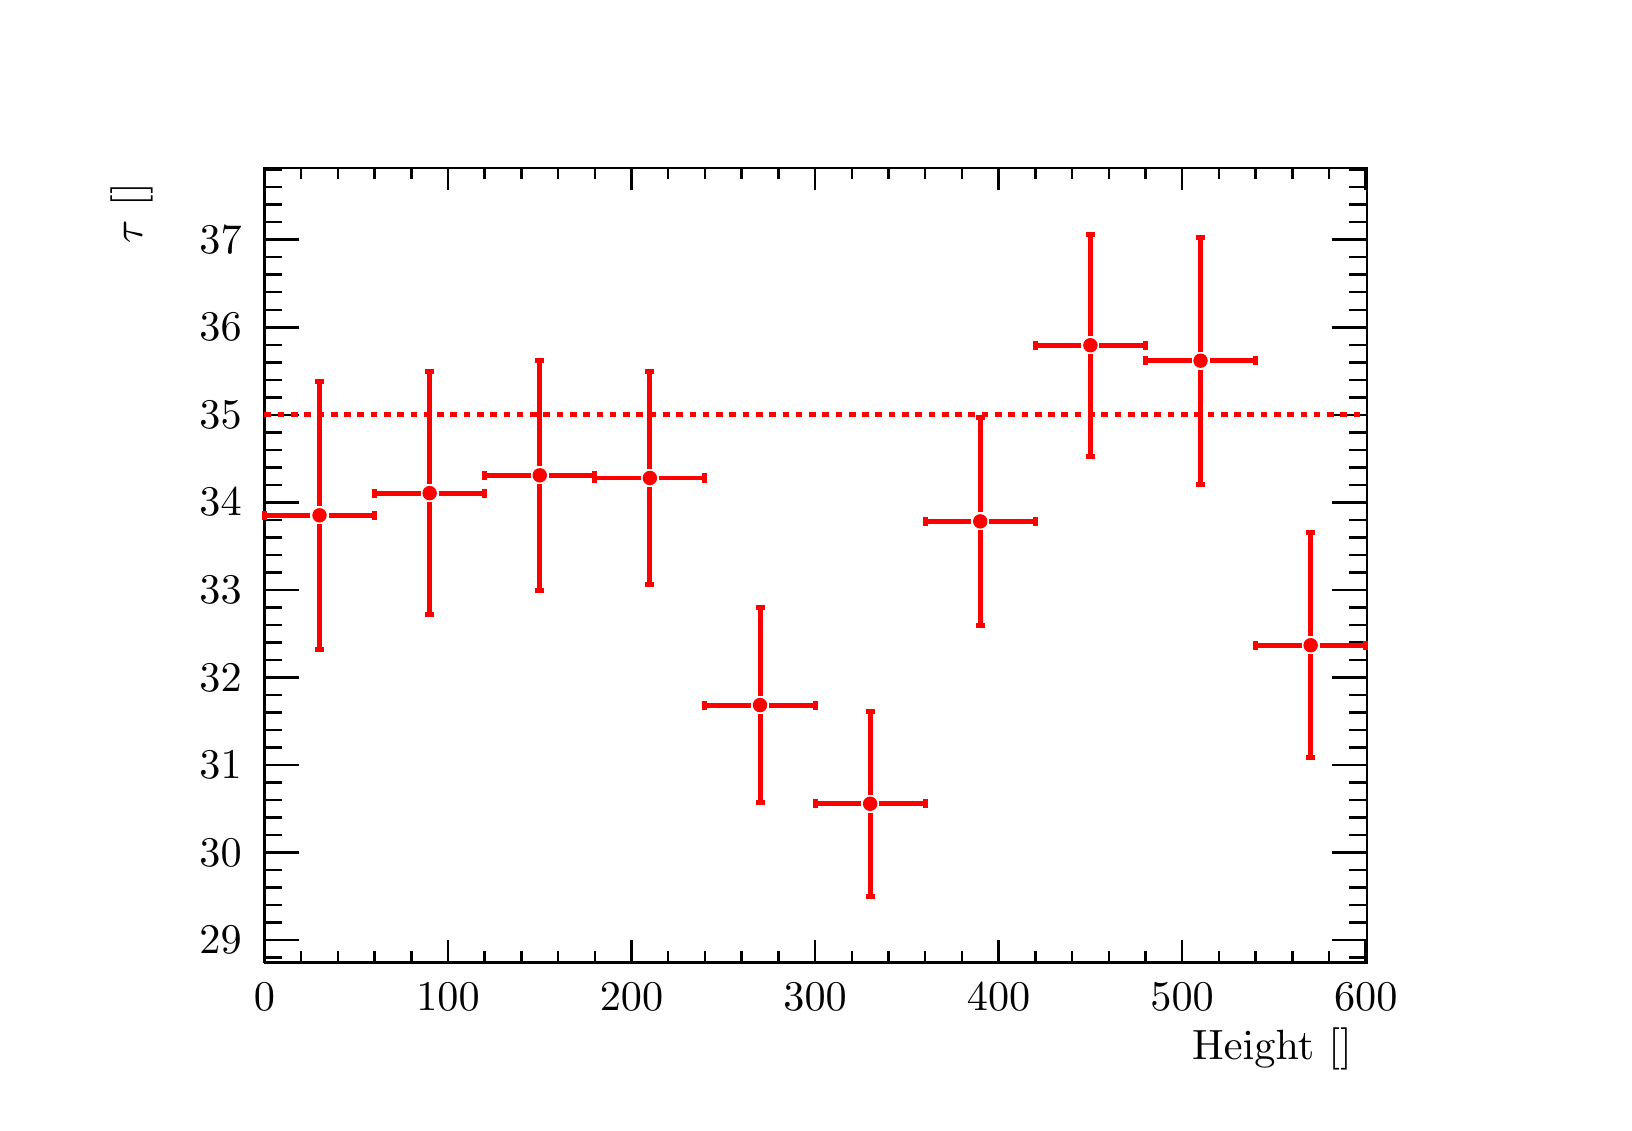
\begin{tikzpicture}
\pgfdeclareplotmark{cross} {
\pgfpathmoveto{\pgfpoint{-0.3\pgfplotmarksize}{\pgfplotmarksize}}
\pgfpathlineto{\pgfpoint{+0.3\pgfplotmarksize}{\pgfplotmarksize}}
\pgfpathlineto{\pgfpoint{+0.3\pgfplotmarksize}{0.3\pgfplotmarksize}}
\pgfpathlineto{\pgfpoint{+1\pgfplotmarksize}{0.3\pgfplotmarksize}}
\pgfpathlineto{\pgfpoint{+1\pgfplotmarksize}{-0.3\pgfplotmarksize}}
\pgfpathlineto{\pgfpoint{+0.3\pgfplotmarksize}{-0.3\pgfplotmarksize}}
\pgfpathlineto{\pgfpoint{+0.3\pgfplotmarksize}{-1.\pgfplotmarksize}}
\pgfpathlineto{\pgfpoint{-0.3\pgfplotmarksize}{-1.\pgfplotmarksize}}
\pgfpathlineto{\pgfpoint{-0.3\pgfplotmarksize}{-0.3\pgfplotmarksize}}
\pgfpathlineto{\pgfpoint{-1.\pgfplotmarksize}{-0.3\pgfplotmarksize}}
\pgfpathlineto{\pgfpoint{-1.\pgfplotmarksize}{0.3\pgfplotmarksize}}
\pgfpathlineto{\pgfpoint{-0.3\pgfplotmarksize}{0.3\pgfplotmarksize}}
\pgfpathclose
\pgfusepathqstroke
}
\pgfdeclareplotmark{cross*} {
\pgfpathmoveto{\pgfpoint{-0.3\pgfplotmarksize}{\pgfplotmarksize}}
\pgfpathlineto{\pgfpoint{+0.3\pgfplotmarksize}{\pgfplotmarksize}}
\pgfpathlineto{\pgfpoint{+0.3\pgfplotmarksize}{0.3\pgfplotmarksize}}
\pgfpathlineto{\pgfpoint{+1\pgfplotmarksize}{0.3\pgfplotmarksize}}
\pgfpathlineto{\pgfpoint{+1\pgfplotmarksize}{-0.3\pgfplotmarksize}}
\pgfpathlineto{\pgfpoint{+0.3\pgfplotmarksize}{-0.3\pgfplotmarksize}}
\pgfpathlineto{\pgfpoint{+0.3\pgfplotmarksize}{-1.\pgfplotmarksize}}
\pgfpathlineto{\pgfpoint{-0.3\pgfplotmarksize}{-1.\pgfplotmarksize}}
\pgfpathlineto{\pgfpoint{-0.3\pgfplotmarksize}{-0.3\pgfplotmarksize}}
\pgfpathlineto{\pgfpoint{-1.\pgfplotmarksize}{-0.3\pgfplotmarksize}}
\pgfpathlineto{\pgfpoint{-1.\pgfplotmarksize}{0.3\pgfplotmarksize}}
\pgfpathlineto{\pgfpoint{-0.3\pgfplotmarksize}{0.3\pgfplotmarksize}}
\pgfpathclose
\pgfusepathqfillstroke
}
\pgfdeclareplotmark{newstar} {
\pgfpathmoveto{\pgfqpoint{0pt}{\pgfplotmarksize}}
\pgfpathlineto{\pgfqpointpolar{44}{0.5\pgfplotmarksize}}
\pgfpathlineto{\pgfqpointpolar{18}{\pgfplotmarksize}}
\pgfpathlineto{\pgfqpointpolar{-20}{0.5\pgfplotmarksize}}
\pgfpathlineto{\pgfqpointpolar{-54}{\pgfplotmarksize}}
\pgfpathlineto{\pgfqpointpolar{-90}{0.5\pgfplotmarksize}}
\pgfpathlineto{\pgfqpointpolar{234}{\pgfplotmarksize}}
\pgfpathlineto{\pgfqpointpolar{198}{0.5\pgfplotmarksize}}
\pgfpathlineto{\pgfqpointpolar{162}{\pgfplotmarksize}}
\pgfpathlineto{\pgfqpointpolar{134}{0.5\pgfplotmarksize}}
\pgfpathclose
\pgfusepathqstroke
}
\pgfdeclareplotmark{newstar*} {
\pgfpathmoveto{\pgfqpoint{0pt}{\pgfplotmarksize}}
\pgfpathlineto{\pgfqpointpolar{44}{0.5\pgfplotmarksize}}
\pgfpathlineto{\pgfqpointpolar{18}{\pgfplotmarksize}}
\pgfpathlineto{\pgfqpointpolar{-20}{0.5\pgfplotmarksize}}
\pgfpathlineto{\pgfqpointpolar{-54}{\pgfplotmarksize}}
\pgfpathlineto{\pgfqpointpolar{-90}{0.5\pgfplotmarksize}}
\pgfpathlineto{\pgfqpointpolar{234}{\pgfplotmarksize}}
\pgfpathlineto{\pgfqpointpolar{198}{0.5\pgfplotmarksize}}
\pgfpathlineto{\pgfqpointpolar{162}{\pgfplotmarksize}}
\pgfpathlineto{\pgfqpointpolar{134}{0.5\pgfplotmarksize}}
\pgfpathclose
\pgfusepathqfillstroke
}
\definecolor{c}{rgb}{1,1,1};
\draw [color=c, fill=c] (0,0) rectangle (20,13.639);
\draw [color=c, fill=c] (3,1.77307) rectangle (17,11.8659);
\definecolor{c}{rgb}{0,0,0};
\draw [c,line width=0.9] (3,1.77307) -- (3,11.8659) -- (17,11.8659) -- (17,1.77307) -- (3,1.77307);
\definecolor{c}{rgb}{1,1,1};
\draw [color=c, fill=c] (3,1.77307) rectangle (17,11.8659);
\definecolor{c}{rgb}{0,0,0};
\draw [c,line width=0.9] (3,1.77307) -- (3,11.8659) -- (17,11.8659) -- (17,1.77307) -- (3,1.77307);
\draw [c,line width=0.9] (3,1.77307) -- (17,1.77307);
\draw [c,line width=0.9] (3,2.05948) -- (3,1.77307);
\draw [c,line width=0.9] (3.4662,1.91628) -- (3.4662,1.77307);
\draw [c,line width=0.9] (3.9324,1.91628) -- (3.9324,1.77307);
\draw [c,line width=0.9] (4.3986,1.91628) -- (4.3986,1.77307);
\draw [c,line width=0.9] (4.8648,1.91628) -- (4.8648,1.77307);
\draw [c,line width=0.9] (5.331,2.05948) -- (5.331,1.77307);
\draw [c,line width=0.9] (5.7972,1.91628) -- (5.7972,1.77307);
\draw [c,line width=0.9] (6.2634,1.91628) -- (6.2634,1.77307);
\draw [c,line width=0.9] (6.7296,1.91628) -- (6.7296,1.77307);
\draw [c,line width=0.9] (7.1958,1.91628) -- (7.1958,1.77307);
\draw [c,line width=0.9] (7.662,2.05948) -- (7.662,1.77307);
\draw [c,line width=0.9] (8.12821,1.91628) -- (8.12821,1.77307);
\draw [c,line width=0.9] (8.59441,1.91628) -- (8.59441,1.77307);
\draw [c,line width=0.9] (9.06061,1.91628) -- (9.06061,1.77307);
\draw [c,line width=0.9] (9.52681,1.91628) -- (9.52681,1.77307);
\draw [c,line width=0.9] (9.99301,2.05948) -- (9.99301,1.77307);
\draw [c,line width=0.9] (10.4592,1.91628) -- (10.4592,1.77307);
\draw [c,line width=0.9] (10.9254,1.91628) -- (10.9254,1.77307);
\draw [c,line width=0.9] (11.3916,1.91628) -- (11.3916,1.77307);
\draw [c,line width=0.9] (11.8578,1.91628) -- (11.8578,1.77307);
\draw [c,line width=0.9] (12.324,2.05948) -- (12.324,1.77307);
\draw [c,line width=0.9] (12.7902,1.91628) -- (12.7902,1.77307);
\draw [c,line width=0.9] (13.2564,1.91628) -- (13.2564,1.77307);
\draw [c,line width=0.9] (13.7226,1.91628) -- (13.7226,1.77307);
\draw [c,line width=0.9] (14.1888,1.91628) -- (14.1888,1.77307);
\draw [c,line width=0.9] (14.655,2.05948) -- (14.655,1.77307);
\draw [c,line width=0.9] (15.1212,1.91628) -- (15.1212,1.77307);
\draw [c,line width=0.9] (15.5874,1.91628) -- (15.5874,1.77307);
\draw [c,line width=0.9] (16.0536,1.91628) -- (16.0536,1.77307);
\draw [c,line width=0.9] (16.5198,1.91628) -- (16.5198,1.77307);
\draw [c,line width=0.9] (16.986,2.05948) -- (16.986,1.77307);
\draw [c,line width=0.9] (16.986,2.05948) -- (16.986,1.77307);
\draw [anchor=base] (3,1.15931) node[scale=1.52731, color=c, rotate=0]{0};
\draw [anchor=base] (5.331,1.15931) node[scale=1.52731, color=c, rotate=0]{100};
\draw [anchor=base] (7.662,1.15931) node[scale=1.52731, color=c, rotate=0]{200};
\draw [anchor=base] (9.99301,1.15931) node[scale=1.52731, color=c, rotate=0]{300};
\draw [anchor=base] (12.324,1.15931) node[scale=1.52731, color=c, rotate=0]{400};
\draw [anchor=base] (14.655,1.15931) node[scale=1.52731, color=c, rotate=0]{500};
\draw [anchor=base] (16.986,1.15931) node[scale=1.52731, color=c, rotate=0]{600};
\draw [anchor= east] (17,0.681948) node[scale=1.52731, color=c, rotate=0]{ Height [\si{\cm}]};
\draw [c,line width=0.9] (3,11.8659) -- (17,11.8659);
\draw [c,line width=0.9] (3,11.5795) -- (3,11.8659);
\draw [c,line width=0.9] (3.4662,11.7227) -- (3.4662,11.8659);
\draw [c,line width=0.9] (3.9324,11.7227) -- (3.9324,11.8659);
\draw [c,line width=0.9] (4.3986,11.7227) -- (4.3986,11.8659);
\draw [c,line width=0.9] (4.8648,11.7227) -- (4.8648,11.8659);
\draw [c,line width=0.9] (5.331,11.5795) -- (5.331,11.8659);
\draw [c,line width=0.9] (5.7972,11.7227) -- (5.7972,11.8659);
\draw [c,line width=0.9] (6.2634,11.7227) -- (6.2634,11.8659);
\draw [c,line width=0.9] (6.7296,11.7227) -- (6.7296,11.8659);
\draw [c,line width=0.9] (7.1958,11.7227) -- (7.1958,11.8659);
\draw [c,line width=0.9] (7.662,11.5795) -- (7.662,11.8659);
\draw [c,line width=0.9] (8.12821,11.7227) -- (8.12821,11.8659);
\draw [c,line width=0.9] (8.59441,11.7227) -- (8.59441,11.8659);
\draw [c,line width=0.9] (9.06061,11.7227) -- (9.06061,11.8659);
\draw [c,line width=0.9] (9.52681,11.7227) -- (9.52681,11.8659);
\draw [c,line width=0.9] (9.99301,11.5795) -- (9.99301,11.8659);
\draw [c,line width=0.9] (10.4592,11.7227) -- (10.4592,11.8659);
\draw [c,line width=0.9] (10.9254,11.7227) -- (10.9254,11.8659);
\draw [c,line width=0.9] (11.3916,11.7227) -- (11.3916,11.8659);
\draw [c,line width=0.9] (11.8578,11.7227) -- (11.8578,11.8659);
\draw [c,line width=0.9] (12.324,11.5795) -- (12.324,11.8659);
\draw [c,line width=0.9] (12.7902,11.7227) -- (12.7902,11.8659);
\draw [c,line width=0.9] (13.2564,11.7227) -- (13.2564,11.8659);
\draw [c,line width=0.9] (13.7226,11.7227) -- (13.7226,11.8659);
\draw [c,line width=0.9] (14.1888,11.7227) -- (14.1888,11.8659);
\draw [c,line width=0.9] (14.655,11.5795) -- (14.655,11.8659);
\draw [c,line width=0.9] (15.1212,11.7227) -- (15.1212,11.8659);
\draw [c,line width=0.9] (15.5874,11.7227) -- (15.5874,11.8659);
\draw [c,line width=0.9] (16.0536,11.7227) -- (16.0536,11.8659);
\draw [c,line width=0.9] (16.5198,11.7227) -- (16.5198,11.8659);
\draw [c,line width=0.9] (16.986,11.5795) -- (16.986,11.8659);
\draw [c,line width=0.9] (16.986,11.5795) -- (16.986,11.8659);
\draw [c,line width=0.9] (3,1.77307) -- (3,11.8659);
\draw [c,line width=0.9] (3.444,2.05957) -- (3,2.05957);
\draw [c,line width=0.9] (3.222,2.2819) -- (3,2.2819);
\draw [c,line width=0.9] (3.222,2.50423) -- (3,2.50423);
\draw [c,line width=0.9] (3.222,2.72656) -- (3,2.72656);
\draw [c,line width=0.9] (3.222,2.94889) -- (3,2.94889);
\draw [c,line width=0.9] (3.444,3.17122) -- (3,3.17122);
\draw [c,line width=0.9] (3.222,3.39355) -- (3,3.39355);
\draw [c,line width=0.9] (3.222,3.61588) -- (3,3.61588);
\draw [c,line width=0.9] (3.222,3.83821) -- (3,3.83821);
\draw [c,line width=0.9] (3.222,4.06054) -- (3,4.06054);
\draw [c,line width=0.9] (3.444,4.28287) -- (3,4.28287);
\draw [c,line width=0.9] (3.222,4.5052) -- (3,4.5052);
\draw [c,line width=0.9] (3.222,4.72752) -- (3,4.72752);
\draw [c,line width=0.9] (3.222,4.94985) -- (3,4.94985);
\draw [c,line width=0.9] (3.222,5.17218) -- (3,5.17218);
\draw [c,line width=0.9] (3.444,5.39451) -- (3,5.39451);
\draw [c,line width=0.9] (3.222,5.61684) -- (3,5.61684);
\draw [c,line width=0.9] (3.222,5.83917) -- (3,5.83917);
\draw [c,line width=0.9] (3.222,6.0615) -- (3,6.0615);
\draw [c,line width=0.9] (3.222,6.28383) -- (3,6.28383);
\draw [c,line width=0.9] (3.444,6.50616) -- (3,6.50616);
\draw [c,line width=0.9] (3.222,6.72849) -- (3,6.72849);
\draw [c,line width=0.9] (3.222,6.95082) -- (3,6.95082);
\draw [c,line width=0.9] (3.222,7.17315) -- (3,7.17315);
\draw [c,line width=0.9] (3.222,7.39548) -- (3,7.39548);
\draw [c,line width=0.9] (3.444,7.61781) -- (3,7.61781);
\draw [c,line width=0.9] (3.222,7.84014) -- (3,7.84014);
\draw [c,line width=0.9] (3.222,8.06247) -- (3,8.06247);
\draw [c,line width=0.9] (3.222,8.28479) -- (3,8.28479);
\draw [c,line width=0.9] (3.222,8.50712) -- (3,8.50712);
\draw [c,line width=0.9] (3.444,8.72945) -- (3,8.72945);
\draw [c,line width=0.9] (3.222,8.95178) -- (3,8.95178);
\draw [c,line width=0.9] (3.222,9.17411) -- (3,9.17411);
\draw [c,line width=0.9] (3.222,9.39644) -- (3,9.39644);
\draw [c,line width=0.9] (3.222,9.61877) -- (3,9.61877);
\draw [c,line width=0.9] (3.444,9.8411) -- (3,9.8411);
\draw [c,line width=0.9] (3.222,10.0634) -- (3,10.0634);
\draw [c,line width=0.9] (3.222,10.2858) -- (3,10.2858);
\draw [c,line width=0.9] (3.222,10.5081) -- (3,10.5081);
\draw [c,line width=0.9] (3.222,10.7304) -- (3,10.7304);
\draw [c,line width=0.9] (3.444,10.9527) -- (3,10.9527);
\draw [c,line width=0.9] (3.444,2.05957) -- (3,2.05957);
\draw [c,line width=0.9] (3.222,1.83724) -- (3,1.83724);
\draw [c,line width=0.9] (3.444,10.9527) -- (3,10.9527);
\draw [c,line width=0.9] (3.222,11.1751) -- (3,11.1751);
\draw [c,line width=0.9] (3.222,11.3974) -- (3,11.3974);
\draw [c,line width=0.9] (3.222,11.6197) -- (3,11.6197);
\draw [c,line width=0.9] (3.222,11.8421) -- (3,11.8421);
\draw [anchor= east] (2.9,2.05957) node[scale=1.52731, color=c, rotate=0]{29};
\draw [anchor= east] (2.9,3.17122) node[scale=1.52731, color=c, rotate=0]{30};
\draw [anchor= east] (2.9,4.28287) node[scale=1.52731, color=c, rotate=0]{31};
\draw [anchor= east] (2.9,5.39451) node[scale=1.52731, color=c, rotate=0]{32};
\draw [anchor= east] (2.9,6.50616) node[scale=1.52731, color=c, rotate=0]{33};
\draw [anchor= east] (2.9,7.61781) node[scale=1.52731, color=c, rotate=0]{34};
\draw [anchor= east] (2.9,8.72945) node[scale=1.52731, color=c, rotate=0]{35};
\draw [anchor= east] (2.9,9.8411) node[scale=1.52731, color=c, rotate=0]{36};
\draw [anchor= east] (2.9,10.9527) node[scale=1.52731, color=c, rotate=0]{37};
\draw [anchor= east] (1.31232,11.8659) node[scale=1.52731, color=c, rotate=90]{$\tau$ [\si{\ms}]};
\draw [c,line width=0.9] (17,1.77307) -- (17,11.8659);
\draw [c,line width=0.9] (16.556,2.05957) -- (17,2.05957);
\draw [c,line width=0.9] (16.778,2.2819) -- (17,2.2819);
\draw [c,line width=0.9] (16.778,2.50423) -- (17,2.50423);
\draw [c,line width=0.9] (16.778,2.72656) -- (17,2.72656);
\draw [c,line width=0.9] (16.778,2.94889) -- (17,2.94889);
\draw [c,line width=0.9] (16.556,3.17122) -- (17,3.17122);
\draw [c,line width=0.9] (16.778,3.39355) -- (17,3.39355);
\draw [c,line width=0.9] (16.778,3.61588) -- (17,3.61588);
\draw [c,line width=0.9] (16.778,3.83821) -- (17,3.83821);
\draw [c,line width=0.9] (16.778,4.06054) -- (17,4.06054);
\draw [c,line width=0.9] (16.556,4.28287) -- (17,4.28287);
\draw [c,line width=0.9] (16.778,4.5052) -- (17,4.5052);
\draw [c,line width=0.9] (16.778,4.72752) -- (17,4.72752);
\draw [c,line width=0.9] (16.778,4.94985) -- (17,4.94985);
\draw [c,line width=0.9] (16.778,5.17218) -- (17,5.17218);
\draw [c,line width=0.9] (16.556,5.39451) -- (17,5.39451);
\draw [c,line width=0.9] (16.778,5.61684) -- (17,5.61684);
\draw [c,line width=0.9] (16.778,5.83917) -- (17,5.83917);
\draw [c,line width=0.9] (16.778,6.0615) -- (17,6.0615);
\draw [c,line width=0.9] (16.778,6.28383) -- (17,6.28383);
\draw [c,line width=0.9] (16.556,6.50616) -- (17,6.50616);
\draw [c,line width=0.9] (16.778,6.72849) -- (17,6.72849);
\draw [c,line width=0.9] (16.778,6.95082) -- (17,6.95082);
\draw [c,line width=0.9] (16.778,7.17315) -- (17,7.17315);
\draw [c,line width=0.9] (16.778,7.39548) -- (17,7.39548);
\draw [c,line width=0.9] (16.556,7.61781) -- (17,7.61781);
\draw [c,line width=0.9] (16.778,7.84014) -- (17,7.84014);
\draw [c,line width=0.9] (16.778,8.06247) -- (17,8.06247);
\draw [c,line width=0.9] (16.778,8.28479) -- (17,8.28479);
\draw [c,line width=0.9] (16.778,8.50712) -- (17,8.50712);
\draw [c,line width=0.9] (16.556,8.72945) -- (17,8.72945);
\draw [c,line width=0.9] (16.778,8.95178) -- (17,8.95178);
\draw [c,line width=0.9] (16.778,9.17411) -- (17,9.17411);
\draw [c,line width=0.9] (16.778,9.39644) -- (17,9.39644);
\draw [c,line width=0.9] (16.778,9.61877) -- (17,9.61877);
\draw [c,line width=0.9] (16.556,9.8411) -- (17,9.8411);
\draw [c,line width=0.9] (16.778,10.0634) -- (17,10.0634);
\draw [c,line width=0.9] (16.778,10.2858) -- (17,10.2858);
\draw [c,line width=0.9] (16.778,10.5081) -- (17,10.5081);
\draw [c,line width=0.9] (16.778,10.7304) -- (17,10.7304);
\draw [c,line width=0.9] (16.556,10.9527) -- (17,10.9527);
\draw [c,line width=0.9] (16.556,2.05957) -- (17,2.05957);
\draw [c,line width=0.9] (16.778,1.83724) -- (17,1.83724);
\draw [c,line width=0.9] (16.556,10.9527) -- (17,10.9527);
\draw [c,line width=0.9] (16.778,11.1751) -- (17,11.1751);
\draw [c,line width=0.9] (16.778,11.3974) -- (17,11.3974);
\draw [c,line width=0.9] (16.778,11.6197) -- (17,11.6197);
\draw [c,line width=0.9] (16.778,11.8421) -- (17,11.8421);
\definecolor{c}{rgb}{1,0,0};
\foreach \P in {(3.6993,7.45301), (5.0979,7.73478), (6.4965,7.96089), (7.8951,7.92679), (9.29371,5.04312), (10.6923,3.78951), (12.0909,7.37598), (13.4895,9.6127), (14.8881,9.4168), (16.2867,5.80286)}{\draw[mark options={color=c,fill=c},mark
 size=2.402402pt,mark=*] plot coordinates {\P};}
\draw [c,line width=1.8] (3.58469,7.45301) -- (3,7.45301);
\draw [c,line width=1.8] (3,7.3957) -- (3,7.51031);
\draw [c,line width=1.8] (3.81391,7.45301) -- (4.3986,7.45301);
\draw [c,line width=1.8] (4.3986,7.3957) -- (4.3986,7.51031);
\draw [c,line width=1.8] (3.6993,7.56762) -- (3.6993,9.15408);
\draw [c,line width=1.8] (3.64199,9.15408) -- (3.75661,9.15408);
\draw [c,line width=1.8] (3.6993,7.33839) -- (3.6993,5.75194);
\draw [c,line width=1.8] (3.64199,5.75194) -- (3.75661,5.75194);
\draw [c,line width=1.8] (4.98329,7.73478) -- (4.3986,7.73478);
\draw [c,line width=1.8] (4.3986,7.67748) -- (4.3986,7.79209);
\draw [c,line width=1.8] (5.21252,7.73478) -- (5.7972,7.73478);
\draw [c,line width=1.8] (5.7972,7.67748) -- (5.7972,7.79209);
\draw [c,line width=1.8] (5.0979,7.8494) -- (5.0979,9.27834);
\draw [c,line width=1.8] (5.0406,9.27834) -- (5.15521,9.27834);
\draw [c,line width=1.8] (5.0979,7.62017) -- (5.0979,6.19122);
\draw [c,line width=1.8] (5.0406,6.19122) -- (5.15521,6.19122);
\draw [c,line width=1.8] (6.38189,7.96089) -- (5.7972,7.96089);
\draw [c,line width=1.8] (5.7972,7.90358) -- (5.7972,8.01819);
\draw [c,line width=1.8] (6.61112,7.96089) -- (7.1958,7.96089);
\draw [c,line width=1.8] (7.1958,7.90358) -- (7.1958,8.01819);
\draw [c,line width=1.8] (6.4965,8.0755) -- (6.4965,9.42201);
\draw [c,line width=1.8] (6.4392,9.42201) -- (6.55381,9.42201);
\draw [c,line width=1.8] (6.4965,7.84627) -- (6.4965,6.49976);
\draw [c,line width=1.8] (6.4392,6.49976) -- (6.55381,6.49976);
\draw [c,line width=1.8] (7.78049,7.92679) -- (7.1958,7.92679);
\draw [c,line width=1.8] (7.1958,7.86948) -- (7.1958,7.9841);
\draw [c,line width=1.8] (8.00972,7.92679) -- (8.59441,7.92679);
\draw [c,line width=1.8] (8.59441,7.86948) -- (8.59441,7.9841);
\draw [c,line width=1.8] (7.8951,8.0414) -- (7.8951,9.2756);
\draw [c,line width=1.8] (7.8378,9.2756) -- (7.95241,9.2756);
\draw [c,line width=1.8] (7.8951,7.81218) -- (7.8951,6.57798);
\draw [c,line width=1.8] (7.8378,6.57798) -- (7.95241,6.57798);
\draw [c,line width=1.8] (9.17909,5.04312) -- (8.59441,5.04312);
\draw [c,line width=1.8] (8.59441,4.98581) -- (8.59441,5.10043);
\draw [c,line width=1.8] (9.40832,5.04312) -- (9.99301,5.04312);
\draw [c,line width=1.8] (9.99301,4.98581) -- (9.99301,5.10043);
\draw [c,line width=1.8] (9.29371,5.15773) -- (9.29371,6.28395);
\draw [c,line width=1.8] (9.2364,6.28395) -- (9.35101,6.28395);
\draw [c,line width=1.8] (9.29371,4.92851) -- (9.29371,3.80229);
\draw [c,line width=1.8] (9.2364,3.80229) -- (9.35101,3.80229);
\draw [c,line width=1.8] (10.5777,3.78951) -- (9.99301,3.78951);
\draw [c,line width=1.8] (9.99301,3.7322) -- (9.99301,3.84681);
\draw [c,line width=1.8] (10.8069,3.78951) -- (11.3916,3.78951);
\draw [c,line width=1.8] (11.3916,3.7322) -- (11.3916,3.84681);
\draw [c,line width=1.8] (10.6923,3.90412) -- (10.6923,4.96488);
\draw [c,line width=1.8] (10.635,4.96488) -- (10.7496,4.96488);
\draw [c,line width=1.8] (10.6923,3.67489) -- (10.6923,2.61414);
\draw [c,line width=1.8] (10.635,2.61414) -- (10.7496,2.61414);
\draw [c,line width=1.8] (11.9763,7.37598) -- (11.3916,7.37598);
\draw [c,line width=1.8] (11.3916,7.31867) -- (11.3916,7.43328);
\draw [c,line width=1.8] (12.2055,7.37598) -- (12.7902,7.37598);
\draw [c,line width=1.8] (12.7902,7.31867) -- (12.7902,7.43328);
\draw [c,line width=1.8] (12.0909,7.49059) -- (12.0909,8.69966);
\draw [c,line width=1.8] (12.0336,8.69966) -- (12.1482,8.69966);
\draw [c,line width=1.8] (12.0909,7.26136) -- (12.0909,6.0523);
\draw [c,line width=1.8] (12.0336,6.0523) -- (12.1482,6.0523);
\draw [c,line width=1.8] (13.3749,9.6127) -- (12.7902,9.6127);
\draw [c,line width=1.8] (12.7902,9.5554) -- (12.7902,9.67001);
\draw [c,line width=1.8] (13.6041,9.6127) -- (14.1888,9.6127);
\draw [c,line width=1.8] (14.1888,9.5554) -- (14.1888,9.67001);
\draw [c,line width=1.8] (13.4895,9.72732) -- (13.4895,11.0248);
\draw [c,line width=1.8] (13.4322,11.0248) -- (13.5468,11.0248);
\draw [c,line width=1.8] (13.4895,9.49809) -- (13.4895,8.20057);
\draw [c,line width=1.8] (13.4322,8.20057) -- (13.5468,8.20057);
\draw [c,line width=1.8] (14.7735,9.4168) -- (14.1888,9.4168);
\draw [c,line width=1.8] (14.1888,9.35949) -- (14.1888,9.4741);
\draw [c,line width=1.8] (15.0027,9.4168) -- (15.5874,9.4168);
\draw [c,line width=1.8] (15.5874,9.35949) -- (15.5874,9.4741);
\draw [c,line width=1.8] (14.8881,9.53141) -- (14.8881,10.9838);
\draw [c,line width=1.8] (14.8308,10.9838) -- (14.9454,10.9838);
\draw [c,line width=1.8] (14.8881,9.30219) -- (14.8881,7.84984);
\draw [c,line width=1.8] (14.8308,7.84984) -- (14.9454,7.84984);
\draw [c,line width=1.8] (16.1721,5.80286) -- (15.5874,5.80286);
\draw [c,line width=1.8] (15.5874,5.74556) -- (15.5874,5.86017);
\draw [c,line width=1.8] (16.4013,5.80286) -- (16.986,5.80286);
\draw [c,line width=1.8] (16.986,5.74556) -- (16.986,5.86017);
\draw [c,line width=1.8] (16.2867,5.91748) -- (16.2867,7.23228);
\draw [c,line width=1.8] (16.2294,7.23228) -- (16.344,7.23228);
\draw [c,line width=1.8] (16.2867,5.68825) -- (16.2867,4.37345);
\draw [c,line width=1.8] (16.2294,4.37345) -- (16.344,4.37345);
\definecolor{c}{rgb}{1,1,1};
\draw [color=c, fill=c] (2,12.8206) rectangle (18,13.5708);
\definecolor{c}{rgb}{0,0,0};
%\draw (10,13.1957) node[scale=1.40004, color=c, rotate=0]{Lifetime vs. height};
\definecolor{c}{rgb}{1,0,0};
\draw [c,dash pattern=on 2.40pt off 2.40pt ,line width=1.8] (3,8.72945) -- (16.986,8.72945);
\end{tikzpicture}

	\end{adjustbox}
	\caption[Measured electron lifetime as a function of height within the detector in simulation]{Measured electron lifetime from cosmic ray tracks as a function of height in the detector for simulation. The simulated lifetime (\SI{35}{\ms}) is shown as the red dotted line.}
	\label{fig:lifetimeNoSCE}
\end{figure}

\subsection{Space charge effects}
\label{sec:pdune_calibration:lifetime:sce}

Previously, it has often been stated that TPCs operate by drifting ionisation electrons across a gap between two charged surfaces.
However, no mention has been made of the corresponding ions produced by the same charged particles when traversing the detector medium.

These positively charged ions will experience the same drift field as the ionisation electrons but will instead drift towards the cathode (rather than the anode).
For a detector medium such as liquid argon, the $\text{Ar}_{2}^{+}$ ions are approximately \num{140000} times heavier than the corresponding electrons and thus will drift much more slowly.
In fact, the ICARUS T600 collaboration reports an argon mobility of \SI{0.9d-3}{\cm\squared\per\volt\per\second}~\cite{icarusSpaceCharge} compared with an electron mobility of around \SI{470}{\cm\squared\per\volt\per\second}~\cite{electronMobility} for electrons.
This slow drifting can lead to a build up of positive ions within the detector and distortions in the applied electric field. 
An analysis of these effects is given in Ref.~\cite{spaceCharge2021}.

ProtoDUNE-SP is vulnerable to space charge effects due to its position on the Earth's surface.
This means that a high constant flux of cosmic rays constantly strikes the detector, producing a steady supply of positive ions which build up and cause distortions from the nominal electric field.
These distortions affect the calorimetric reconstruction in multiple ways.
Firstly, distortions in the electric field result in changes to the drift velocity of ionisation electrons which must be accounted for in order to correctly calculate track segment lengths when measuring \dqdx.
Secondly, as shown in \citefig{fig:recombFactors} the applied electric field in a TPC affects the number of ionisation electrons which recombine. 
Therefore, any change in the electric field will alter the amount of charge liberated by a charged particle which is then free to drift to the readout planes.

In order to correct for these effects, maps of the effective electric field (including contributions from space charge) and spatial distortions are constructed.
These distortions are evaluated by taking exiting tracks and measuring the offsets between the reconstructed end points and the TPC faces
These are used to generate a data-driven simulation of the space charge effects which can then be inverted to provide corrections for said effects~\cite{protodunePerformance}.
Two-dimensional slices of the three-dimensional electric field distortion map for ProtoDUNE-SP data are shown in \citefig{fig:eFieldDistortion}. 
Here, one can see that the magnitude of the electric field is changed at some points by as much as 25\%.

\begin{figure}[h]
	\centering
	\includegraphics[width=.9\linewidth]{files/figures/protodune_calibration/eFieldDistortion}
	\caption[Two-dimensional slices of the three-dimensional electric field distortion map in ProtoDUNE-SP data]{Two-dimensional slices of the three-dimensional electric field distortion map in ProtoDUNE-SP data, from~\cite{protodunePerformance}. Left: A slice taken at constant $Z$. Right: A slice taken at constant $Y$.}
	\label{fig:eFieldDistortion}
\end{figure}

\subsection{Results from data}
\label{sec:pdune_calibration:lifetime:data}

The process detailed above is repeated for multiple data runs.
In each case the calorimetry is corrected for space charge effects (SCE). 
This effect and its corrections are detailed in \citesec{sec:pdune_calibration:lifetime:sce}.

\section{Impact on far detector measurements}
\label{sec:pdune_calibration:fd}